%
%  User's guide for the software library  TestU01
%
\documentclass[12pt]{report}
\usepackage{url}
\usepackage{makeidx}
\usepackage{verbatim}
\usepackage{supertabular}

% The symbols for the complex, the real, the integers, the fields.
\usepackage{amssymb}
%% $\mathbb{C, R, N, Z, F}$

\input ../doc/myarticle.sty

\def\myboxit#1{\vbox{\hrule height1pt
                   \hbox{\vrule width1pt\kern10pt
                         \vbox{\kern3pt#1\kern3pt
                              }\kern10pt\vrule width1pt
                        }\hrule height1pt }}

\makeindex

\def\To {\Rightarrow}
\def\o {{(o)}}
\newcommand\cH{\mathcal{H}}
\def\bv  {{\bf v}}
\def\bx  {{\bf x}}
\def\bA  {{\bf A}}
\def\bI  {{\bf I}}
\def\bL  {{\bf L}}
\def\bR  {{\bf R}}
\def\tpose{^{\sf T}}

\newcommand\guisec[1]{\vspace{20pt}%
\noindent\hrulefill\hspace{10pt}{\bf #1}\hspace{10pt}\hrulefill%
\nopagebreak\vspace{10pt}}

\newcommand{\DelGen}{Frees the dynamic memory used by any generator
  returned by the {\tt Create} functions of this module.
  This function should be called to clean up any generator object of this
  module when it is no longer in use.}

\newcommand{\resdef}{The parameter {\tt res} is usually set to the
 {\tt NULL} pointer.
However, if one wants to examine or post-process the results after a
test, then one must explicitly create a  {\tt res} structure.
\ifdetailed \else
See the detailed version of this guide for the definition of the
structures and the relevant instructions.\fi\bigskip}

\newtheorem {theorem}{Theorem}
\newtheorem {proposition}{Proposition}
\newtheorem {lemma}{Lemma}
\newtheorem {corollary}{Corollary}
\newtheorem {assumption}{Assumption}
\newtheorem {example}{Example}

% \def\pierre#1 {\fbox {\footnote {\ }}\ \footnotetext { From Pierre: #1}}
\def\richard#1 {\fbox {\footnote {\ }}\ \footnotetext { From Richard: #1}}
\def\hpierre#1{}
\def\hrichard#1{}
\def\myurl{\url{http://www.iro.umontreal.ca/~lecuyer}}
\def\mycode{\code}
\def\myendcode{\endcode}

%%%%%%%%%%%%%%%%%%%%%%%%%%%%%%%
% Switch to get a more/less detailed version of the user's guide.

\newif\ifdetailed\detailedfalse
\newenvironment{detailed}{\protect\ifdetailed }{\protect\fi }
% \detailedtrue   % For a more detailed user's guide.

% \includeonly {bbattery}

%%%%%%%%%%%%%%%%%%%%%%%%%%%%%%%%
\begin {document}
\begin {titlepage}

\null 
\begin {flushright} \it This version: \today \end {flushright}

\vfill
\begin{center}
 {\Large\bf TestU01} \\ \ \\
 {\large\bf A Software Library in ANSI C \\[6pt]
    for Empirical Testing of Random Number Generators}\\
\vfill
{\bf   User's guide, 
 \ifdetailed  detailed version \else compact version \fi }
\vfill
 Pierre L'Ecuyer and Richard Simard \\[10pt]
D\'epartement d'Informatique et de Recherche Op\'erationnelle \\
Universit\'e de Montr\'eal \\
\end{center}
\vfill

This document describes the software library {\em TestU01}, 
implemented in the ANSI C language,
and offering a collection of utilities for the (empirical)
statistical testing of uniform random number generators (RNG).

The library implements several types of generators in
generic form, as well as many specific generators proposed in
the literature or found in widely-used software.
It provides general implementations of the classical statistical tests
for random number generators, as well as several others proposed in the
literature, and some original ones.
These tests can be applied to the generators predefined in the library
and to user-defined generators.
Specific tests suites for either sequences of uniform random numbers
in $[0,1]$ or bit sequences are also available.
Basic tools for plotting vectors of points produced by generators
are provided as well.

Additional software permits one to perform
systematic studies of the interaction between a specific test
and the structure of the point sets produced by a given family of RNGs.
That is, for a given kind of test and a given class of RNGs, 
to determine how large should be the sample size of the test,
as a function of the generator's period length, 
before the generator starts to fail the test systematically.

\vfill
\end{titlepage}



\pagenumbering{roman}
\section*{Copyright}
 
%\begin{verbatim}
  Copyright \copyright {} 2002 by Pierre L'Ecuyer,
    Universit\'e de Montr\'eal.\\
  Web address:   \url{http://www.iro.umontreal.ca/~lecuyer/} \\
  All rights reserved.
 
\noindent  Redistribution and use in source and binary forms, with or without
  modification, are permitted without a fee for private, research,
  academic, or other non-commercial purposes.
  Any use of this software in a commercial environment requires a
  written licence from the copyright owner.
 
\noindent  Any changes made to this package must be clearly identified as such.
 
\noindent  In scientific publications which used this software, a reference to it
  would be appreciated.
 
\noindent  Redistributions of source code must retain this copyright notice
  and the following disclaimer:
 
\noindent  THIS PACKAGE IS PROVIDED ``AS IS'' AND WITHOUT ANY EXPRESS OR
  IMPLIED WARRANTIES, INCLUDING, WITHOUT LIMITATION, THE IMPLIED
  WARRANTIES OF MERCHANTIBILITY AND FITNESS FOR A PARTICULAR PURPOSE.
%\end{verbatim}

\addcontentsline{toc}{chapter}{Copyright}
\tableofcontents
\clearpage

\pagenumbering{arabic}

\chapter{Introduction to Mesquite} \label{sec:intro}

\section{Overview of Mesh Quality}

\hskip 0.25in {\it Mesh quality} refers to geometric properties of a mesh such as
local volume, smoothness, shape, and orientation that, if not properly
controlled,
can adversely affect solution accuracy or computational efficiency of numerical simulations. In this section we give an overview of the role of mesh quality
in the context of computer simulations of physical phenomena. \newline

Simulation of many phenomena in the physical world involves computing
numerical
solutions to partial differential equations (PDE's). Commonly used approaches
to computing  numerical solutions such as finite volume and finite
element methods require the use of approximations to the continuum operators
in the PDE and a mesh or grid to subdivide the physical domain into small
subregions. Together, the approximations and the mesh define a discretization.
The difference between the exact solution to the PDE and the numerical solution is known as the discretization error. A {\it convergent}
discretization means that the discretization error will asymptotically
approach zero as the characteristic mesh size ``h''
approaches zero. Decreasing mesh size to reduce discretization error to
nearly zero is often impractical in realistic simulations due to limited
computing resources. One way to increase the accuracy of simulations with the
same computer resources is to {\it adapt} the mesh to the domain and to the
numerical solution. In adaptive refinement, the local mesh volume (or size)
is made smaller in locations where the local discretization error is large and
is made larger in locations where the error is small. In local h-refinement,
mesh volume is made smaller by locally subdividing the mesh. In
r-refinement, mesh volume is made smaller by moving mesh nodes closer together.
Geometric adaptation can also be important in improving simulation accuracy. In regions of high domain curvature one adapts the mesh to the domain geometry by creating locally smaller mesh sizes. We see, then, that local mesh size (or volume) is a critical parameter in determining the accuracy of a simulation. \newline

Aside from local mesh size, several other geometric mesh properties can affect
solution accuracy. These include mesh smoothness, local mesh angles, aspect
ratio, and orientation. For example, in some discretization methods there will be a
loss of accuracy if the mesh is not smooth.  In other cases, aspect ratios and
orientation must be carefully adapted to the solution in order to maintain a
certain level of accuracy. Simulations using meshes or domains that evolve
in time (such as in ALE simulations) usually require that initially good
geometric mesh properties be retained throughout the simulation time period.
It is thus often important to control other geometric mesh properties in addition to local mesh size within an adaptive simulation. \newline

In addition to solution accuracy, geometric mesh properties can also affect the amount of computer time required to obtain the numerical solution. Simulation codes usually employ iterative solvers to solve systems of equations and thus obtain numerical solutions to PDE's. The rate at which these solvers converge is determined by the spectral radius of a certain matrix. The spectral radius of the matrix is affected by, among other things, geometric properties of the mesh. Poor mesh quality can thus adversely impact solution efficiency. \newline

Adaptive meshing techniques require an initial mesh to begin the adaptation procedure. Poor quality of the initial mesh (relative to the adapted mesh) can be difficult to overcome or, at least, reduce the efficiency of
the adaptive procedure. For example, if the initial mesh contains locally inverted elements, these can often be fixed before the adaptive procedure begins. As another example, if it is known \`{a} priori that small angles will be needed on the boundary of the domain to obtain reasonable simulation accuracy, one should try to first create the small angles in the initial mesh to improve the efficiency of the subsequent adaptive meshing procedure. \newline


Many simulations, particularly those in industry, are performed in a
non-adaptive setting. That is to say, an initial mesh is generated and
used throughout the calculation. The mesh is not changed as the solution
is computed. Mesh quality remains important for such calculations. First,
for complicated geometric domains it is often difficult to obtain good
initial mesh quality. This is particularly true for non-simplicial meshes
but can be true for simplicial meshes as well. A common requirement is that the mesh be smooth. Many simulation codes will not run to completion if the initial mesh contains a local volume which is negative. These must be eliminated before a simulation can begin. Analysts performing
non-adaptive calculations often have considerable experience in using a variety
of meshes on their problem and have a good \`{a} priori idea of what constitutes
good mesh quality for a given problem. They thus desire to control the usual
geometric mesh properties of the non-adapted mesh carefully.



\section{How Mesh Quality Is Improved}
Mesh quality can and should be considered during many stages of
the mesh generation process from de-featuring CAD models to
creation and adaptation of the mesh. Thus, for example, certain
non-essential features of a CAD model, if eliminated, would go a
long way to improving the quality of the mesh, depending upon
the meshing scheme. Other critical meshing parameters which can
affect mesh quality include geometric domain partitions, interval size
and count, interaction of meshes within large assemblies of parts,
biasing requirements, corner picking, etc. Choices made during the
mesh generation phase of an analysis may have a large impact on
initial mesh quality.  Mesh quality can thus be improved by changing the
way in which the domain is meshed. \newline

Once the meshing stage is completed, one can improve mesh quality
by techniques such as vertex movement and local topology modification.
In vertex movement schemes, one seeks to reposition existing mesh vertices to
achieve better quality. If vertex movement is undertaken within an adaptive
setting, it is commonly referred to as r-refinement.
Classic examples of vertex movement methods
include Laplace smoothing \cite{F88} and Winslow smoothing \cite{Winslow}.
It is helpful, in vertex movement schemes, to first be
able to measure mesh quality so that one can explain in what sense one
has improved it. Given a {\it metric} to measure mesh quality,
one can formulate a numerical
optimization problem which guides vertex movement to find the optimal
mesh and thus improve its quality.  Numerical
optimization methods recently
developed for unstructured meshes include \cite{Opt-MS,Kn00,FrKn01,
FeasNewt,bjoe:swap,bjoe:chain-swap,es92}. \newline
%We refer the reader to ref xxx
%which is a survey of mesh quality improvement methods which have appeared
%in the literature. \newline

A large number of mesh quality metrics have been devised to measure
mesh quality. Many of these metrics are independent of any solution
properties and are thus not useful in adaptive meshing. However, there
are a number of weighted quality metrics which can be tied to the
numerical solution via error indicators or other information for adaptive
meshing. \newline
%Examples of weighted metrics which have or could be used in
%adaptive calculations include those of Brackbill (ref), Knupp (ref), etc. \newline

Another way to improve mesh quality is to use local topological modification methods in which mesh vertices or elements are locally created and/or destroyed. These methods are very successful when applied to simplicial meshes, often within an adaptive context.  Local topology modification is less effective on non-simplicial meshes. \newline

Mesh quality improvement remains an important on-going research area.
There remain, for example, open questions with regard to metrics which
can be used in adaptive settings, theoretical questions on problem
formulation, and how to obtain improved meshes quickly. An important
subset of Mesquite capabilities is based on a mathematical theory that we
are developing which we call the Target-matrix paradigm (TMP).  The
basic idea is similar to that from Harmonic mappings, as applied to mesh
generation: use only a few very soundly formulated quality metrics and
adapt the mesh to a wide variety of specialized purposes via specification
of the mapping on the target manifold. However, TMP is formulated as a
discrete optimization problem, which allows direct control over important
properties such as invertibility which must hold even if the asympototic limit
is not reached. The mathematics behind the Target-matrix
paradigm can be found in \cite{formal,local2dmetrics,convexity,analysis2D,labelinv,labelinv-imr,tgtcons}. \newline

Although mesh quality improvement algorithms have been widely implemented
in both meshing and applications codes, it has always been difficult to
improve the quality of a mesh created in one software package using an
improvement algorithm which has been implemented in another.  This difficulty
and others have inspired the creation of the Mesquite software library.
This library is described in the next section. \newline


\section{Mesquite Goals}
Mesquite (Mesh Quality Improvement Toolkit) is designed to provide a
stand-alone, portable, comprehensive suite of mesh quality improvement
algorithms and components that can be used to construct custom quality
improvement algorithms.
The design is flexible so that the algorithms can be applied to many
different mesh element types and orders and referenced to both
isotropic and anisotropic ideal elements.  Mesquite provides a robust
and effective mesh improvement toolkit that allows both meshing
researchers application scientists to benefit from the latest
developments in mesh quality control and improvement. \newline

Mesquite design goals are derived from a mathematical framework and
are focused on providing a versatile, comprehensive, inter-operable,
robust, and efficient library of mesh quality improvement algorithms
that can be used by the non-expert and extended and customized by
experts.  In this section we highlight the current status of Mesquite
in several of our design goal areas. \newline


{\bf Versatile.}  Mesquite works on structured, unstructured, and
hybrid meshes in both two and three dimensions. The design permits
improvements to meshes composed of triangular, tetrahedral,
quadrilateral, hexahedral, prismatic (wedge) and pyramidal elements.
Support for general polyhedral elements may be added at a future time.
It currently incorporates
only methods for node movement; plans for topology modification and
hybrid improvement strategies lie in the future.  Node movement
strategies include both local patch-based iteration schemes for one or
a few free vertices and global objective functions which improve all
vertices simultaneously. Mesquite will be applicable to both adaptive
and nonadaptive meshing and to both low- and high-order discretization
schemes, but currently works with non-adaptive meshes containing
linear elements. \newline

{\bf Comprehensive.}  Mesquite will address a large variety of mesh
quality improvement goals including mesh volume control (sizing,
invertibility), mesh angles, aspect ratios, and orientation. Specific
goals include mesh untangling, mesh smoothing, shape improvement,
anisotropic smoothing, mesh rezoning for ALE, mesh alignment, and
deforming mesh algorithms. These goals can be pursued in both adaptive
and non-adaptive settings. The software is customizable, enabling
users to insert their own quality metrics, objective functions, and
algorithms and also provides mechanisms for creating combined
approaches that use one or more improvement algorithms. \newline

%{\bf Effective.}  Mesquite uses state-of-the-art algorithms and
%metrics to guarantee improvement in mesh quality.  Because the
%definition of mesh quality is application specific, we provide quality
%metrics that allow the user to untangle meshes, improve mesh
%smoothness, element size, and shape. In the future these metrics will
%be referenced to permit non-isotropic smoothing and adaptivity. \newline

{\bf Inter-operable.}  To ensure that Mesquite is inter-operable with a
large number of mesh generation packages, Mesquite defines a generic
interface for accessing application mesh and domain data.  Additoinally,
Mesquite provides an adapter to interface with the common
interfaces for mesh and geometry query currently under developed by the
ITAPS center.  These interfaces provide uniform access to mesh geometry and
topology and will be implemented by all ITAPS center software including
several DOE-supported mesh generation packages.  We are working with
the ITAPS interface design team to ensure that Mesquite has efficient
access to mesh and geometry information through strategies such as
information caching and agglomeration.  We are also participating in
the design of interfaces needed to support topological changes
generated by mesh swapping and flipping algorithms and to constrain
vertices to the surface of a geometrical model. \newline

{\bf Efficient.}  The outer layers of Mesquite use
object-oriented design in C++ while the inner kernels use
optimizable coding constructs such as arrays and inlined
functions.  To ensure efficient use of computationally intensive
optimization algorithms, we employ inexpensive smoothers, such as
Laplacian smoothing, as ``preconditioners'' for the more expensive
optimization techniques.  In addition, mesh culling algorithms can be
used to smooth only those areas of the mesh that require improvement.
Considerable attention has been devoted to understanding and
implementing a variety of termination criteria that can be used to
control the computational cost of the optimization algorithms. \newline

{\bf Robust.} Sound software engineering principles and robust numerical
algorithms are employed in Mesquite.
%Code interrupts due to null pointers and zero-divides will be handled gracefully.
A comprehensive suite of test problems and a unit testing framework have
been developed to verify the correct execution of the code. \newline

Mesquite is not intended to be a mesh generation tool. It can serve as
a post-processor to a mesh generation procedure, a mesh pre-processor to a
non-adaptive simulation code, or as an algorithm for in-core adaptive mesh
quality improvement. As a software library, Mesquite is intended to be
linked to either a meshing code or to a simulation code. \newline

\section{Mesquite Concepts} \label{sec:concepts}

Mesquite software design is based on a mathematical
framework that improves mesh quality by solving an optimization
problem to guide the movement of mesh vertices. The user inputs a mesh or
submesh consisting of vertices, elements, and the relationships between them.
The quality of each vertex or
element in the mesh is described by a local quality metric that is a function
of a subset of the mesh vertices. The global quality of the mesh is formed by
taking the global norm or the average of the local mesh qualities. The global
quality is thus a function of the positions of all the mesh vertices. If this
function can be used in a well-posed minimization problem (e.g., it is
bounded below and has one or more local minimums), mesh vertices are moved
by Mesquite toward the vertex positions of the optimal mesh, thus improving
the quality according to the criterion defined by the local quality metric.
By changing the local quality metric one can achieve a variety of mesh quality improvement goals such as mesh untangling, shape improvement, and size adaptation. \newline

Users of Mesquite should have in mind a goal or set of goals which define
the quality of the mesh which is to be improved. The goal determines which
quality metric or metrics one will use in the optimization problem. Other
user inputs will include an objective function template which describes
the norm or average they wish to use in defining the global mesh quality.
For example, an L-infinity norm will tend to improve the worst-case local
quality while an L-2 norm will improve the RMS quality of the global mesh.
Once the global quality (objective function) is defined, the user can
select a numerical optimization scheme (solver) within Mesquite such as a
steepest descent, conjugate gradient, or feasible Newton method. A variety of
termination criteria can be selected singly or in combination to tell the
solver when to halt. These are useful in controlling the trade-off between
the accuracy of the minimization procedure vs. how much CPU is consumed.
There is also an important flag that determines whether the optimization
problem will be solved via a succession of optimizations on local patches
followed by a complete pass over the global mesh or if it will be solved using
a global patch in which all mesh vertices are moved simultaneously. Advantages
and disadvantages of each of these approaches is currently under study.\newline

Sometimes hybrid mesh optimization schemes are useful, for example, in
first untangling a mesh and then improving the shape of its elements. For
sequences of optimization problems Mesquite uses the concept of an
instruction queue.  The queue determines the order in which the optimization
problems are solved, using the output from the previous optimization step
as the input to the next optimization step. The queue defines a master
quality improver that defines the ultimate mesh quality improvement goal.
The queue can also be used to include steps to assess mesh quality say
before and after each optimization step within the queue.  The quality
assessor measures various aspects of quality in the mesh and may include
other quality metrics besides the one used to define the optimization problem.
\newline

Optimization problems can be solved directly by minimizing the objective
function or indirectly by positioning mesh vertices at a stationary point
of the global objective function. Stationary points are defined by setting
the gradient of the objective function to zero. The indirect method is akin
to iteratively solving a system of linear (or nonlinear) equations.
Currently, such systems are solved in Mesquite and other mesh quality
software by using the local patch method that is akin
to a Gauss-Seidel iteration. The prime example of this in Mesquite is
Laplace smoothing. In the
future we may include methods for solving global systems of equations
in Mesquite to obtain solutions more quickly.
In the past, some mesh smoothing algorithms have been formulated as a
local iterative method that cannot be derived
by setting the gradient of an objective function to zero. Such methods are
frowned upon in Mesquite since one cannot state what mesh quality metric is
improved.  However, if such methods are included in future versions of Mesquite, they will be done in a manner similar to the local Laplace smoothing
algorithm in Mesquite. \newline

%\noindent The following notation is used in the rest of this manual
%\begin{itemize}
%\item The mesh is assumed to consist of $N$ elements and $M$ free vertices.
%Let $n=1,2,\ldots,N$.
%\item Let $q$ be a scalar which defines an element-based {\it quality} metric.
%The quality of the $n^{th}$ element in the mesh is given by the scalar
%$q_n$. Element quality is a function of the coordinates ${\bf x}_n$
%of the vertices belonging to the element, i.e., $q_n = q({\bf x}_n)$
%\item Let $Q \in R^N$ be the vector $[q_1,q_2,\ldots,q_n]$ of element
%qualities over the mesh. Let $f$ be a function from $R^N$ to $R$. When
%$f$ is applied to $Q$, we call $f(Q)$ an {\it objective function template}.
%\item Because each of the element qualities depends on the coordinates of
%the vertices which it contains, the vector $Q$ is a function of the coordinates
%of all of the free vertices ${\bf x} \in R^{3M}$ in the mesh, i.e., $Q=Q({\bf x})$. Finally, form $F({\bf x})= f \circ Q({\bf x}) = f(Q({\bf x}))$ as a
%function from $R^{3M}$ to $R$.  The function $F$ is the mesh quality
%{\it objective function}.
%\item $\nabla F \in R^{3M}$ is the {\it gradient} of the objective function
%with respect to the coordinates of the free vertices. Let ${\cal H} F= \nabla (\nabla F)$ be the {\it Hessian} of the objective function.  The Hessian is a
%$3M \times 3M$ matrix.
%\end{itemize}

\begin{figure}[htb]
\begin{center}
%\begin{tabular}{c}
%\psfig{figure=./msq-paradigm.eps,width=4.7in}
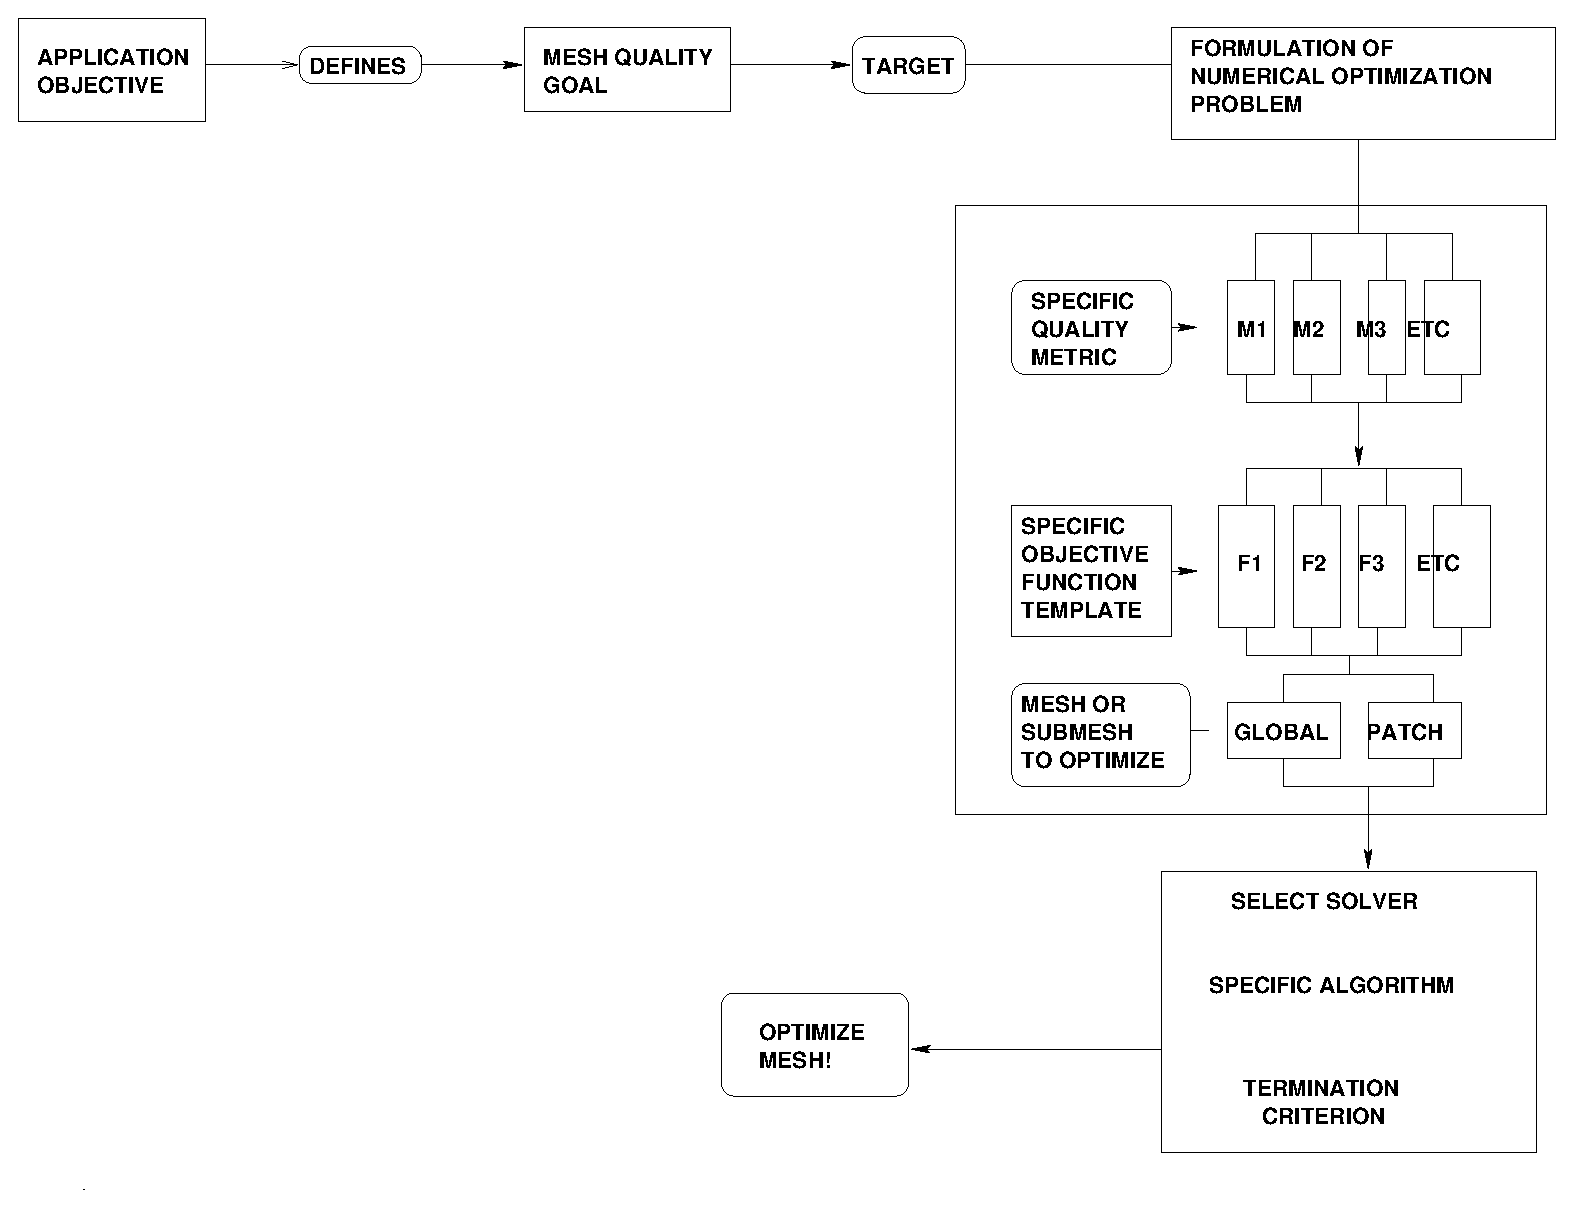
\includegraphics[width=4.7in]{figures/msq-paradigm}
\caption{\em The Mesquite Paradigm \label{Paradigm} }
%\end{tabular}
\end{center}
\end{figure}

\section{How to use this User's Manual}
This user's manual
\begin{itemize}
\item provides an introduction to mesh quality and basic Mesquite concepts (Chapter \ref{sec:intro}),
\item instructs novice users on how to download and install Mesquite (Chapter \ref{sec:install}),
\item provides a tutorial on Mesquite's simplified user's interface and Mesquite's detailed API (Chapter \ref{sec:examples}).
\item describes how to load a mesh in Mesquite via files (Chapter \ref{sec:meshes}), and
%\item provides instructions on using the extensive TSTT interface or a Mesquite mesh specific mesh
%      interface to load a mesh {\it dynamicallu} in Mesquite (sections \ref{sec:msq_mesh}, \ref{sec:TSTT}), and
\item describes Mesquite interactions with domain geometry (Chapter \ref{sec:geom}), and
\item describes Mesquite Wrappers (Chapter \ref{sec:wrappers}),
%\item Exposes in details the concepts and the mechanisms of the advanced API (chapter \ref{sec:API}), and
%\item instructs the user on how to add their own instances of quality
%metrics, objective functions, and solvers (chapter \ref{sec:extensions})
\end{itemize}

Consult the doxygen documentation for the API reference as well as details on the software. There
are two sets of doxygen documentations available:
\begin{itemize}
\item The developer doxygen doc is located in mesquite/doc/developer/. From that directory, you
      must run 'doxygen Mesquite.dox'.
\item The user doxygen doc (API doc) is located in mesquite/doc/user/doxygen. From that directory, you
      must run 'doxygen Mesquite-user.dox'.
\end{itemize}
The doxygen command will generate two directories: an html directory containing the file
index.html that you can open with your web browser, and a latex directory containing a Makefile that
will generate a dvi file.

%\section{Related Documents}

%Documentation of the Mesquite API can be generated from comments in the Mesquite
%source code using the Doxygen utility
%(\url{http://www.stack.nl/~dimitri/doxygen/}).
%To generate HTML and LaTeX copies of this documentation, execute the command
%{\tt doxygen Mesquite-user.dox} in the {\tt doc/usr/doxygen} subdirectory
%of the Mesquite source.

%Further information and related documentation are available on the
%Mesquite home page, located at:
%\url{http://www.cs.sandia.gov/optimization/knupp/Mesquite.html}.

\chapter{UNIFORM GENERATORS}

This chapter contains a description of various uniform generators
already programmed in this library and which were proposed by various 
authors over the past several years, as well as tools for managing
and implementing additional types of generators.
Related generators are regrouped in the same module.
For example, the linear congruential generators (LCGs) are in module
{\tt ulcg}, the multiple recursive generators (MRGs) are in {\tt umrg}, 
the inversive generators in {\tt uinv},
the cubic generators in {\tt ucubic}, etc.
We emphasize that the generators provided here are not all recommendable;
in fact, {\em most of them are not}.

The module {\tt unif01} contains the basic utilities for defining,
manipulating, filtering, combining, and timing generators.  
Each generator must be implemented as an 
object of type {\tt unif01\_Gen}.  To implement one's own generator,
one should create such an object and define all its fields.
For each generator, the structure {\tt unif01\_Gen} must contain a 
function {\tt GetU01} that returns values in the interval $[0,1)$
and a function {\tt GetBits} that returns a block of 32 bits.  
Most of the tests in the {\tt s} modules call the generators
to be tested only indirectly, through the use of the interface 
functions {\tt unif01\_StripD}, {\tt unif01\_StripL} and  
{\tt unif01\_StripB}.
These functions drop the $r$ most significant bits of each random number 
generated and returns a number built out of the remaining bits.

It is also possible to test one's own or an external generator
(that is, a generator that is not predefined in TestU01) very easily with
the help of the functions {\tt unif01\_CreateExternGen01} and
{\tt unif01\_CreateExternGenBits} (see page \pageref{externgen}
of this guide), as long as this generator is programmed in C.

Figure~\ref{fig:usegen} gives simple examples of how to use predefined
generators.  The program creates a LCG with modulus $m = 2^{31}-1$,
multiplier $a = 16807$, and initial state $s = 12345$,
generates and adds 100 uniforms produced by this generator,
prints the sum, and deletes the generator.
To illustrate the fact that there are different ways of getting the
uniforms from the generator, we have generated the first 50 by calling
the {\tt GetU01} function and the next 50 via {\tt unif01\_StripD}.
These two methods are equivalent.
The program then instantiates the generator {\tt lfsr113} available in 
module {\tt ulec}, with the vector $(12345, \ldots, 12345)$ as initial seed,
generates and prints five integers in the range $\{0,\dots,2^{10}-1\}$
(i.e., 10-bit integers) obtained by taking five successive output values
from the generator, stripping out the four most significant bits from 
each value, and retaining the next 10 bits.

For each public identifier used in programs, it is important to
include the corresponding header file before using it,
so as to inform the compiler about the type and signature of functions
and exported variables. For instance, in the following examples, the header
files \texttt{unif01.h}, \texttt{ulcg.h} and \texttt{ulec.h} contain the 
declarations of \texttt{unif01\_Gen}, \texttt{ulcg\_CreateLCG} and 
\texttt{ulec\_Createlfsr113}, respectively.
 
Other examples on how to use the facilities of module {\tt unif01} are given 
at the end of its description.


\setbox0=\vbox {\hsize = 6.0in
\smallc
\verbatiminput{../examples/ex1.c}
}

\begin{figure}
\centering
\myboxit{\box0}
\caption {Using pre-programmed generators\label {fig:usegen}}
\end{figure}


\iffalse  %%%%%%%
%%%%%%%%%%%%%%%%%%%%%%%%%%%%%%%%%%%%%%%%%%%%%%%%%%%%%%%%%%%%%%%

\section {La vitesse des generators}

Les Tableaux \ref{vitesse1}--\ref{vitesse10} donnent une idee 
du temps d'execution moyen
par appel (en micro-secondes), pour un certain number de generators
fournis par the modules {\tt u...}.
Ces values sont en fait le number de secondes
requises pour un million $(10^6)$ d'appels, 
donne ici a une seconde pres.
La machine utilisee etait un SUN UltraSparc 150.
%%  80386 avec coprocesseur 80387, tous deux a 16 MHz.
Pour fins de comparaison, pour un million d'appels a une procedure
``bidon'' ne faisant rien, dans le m\^eme contexte, il a fallu 0.26 secondes.

\begin{table}[htb] \centering \tt
\caption {\rm Vitesse moyenne par appel pour the generators 
          du module ulcg.}
\label {vitesse1}
\begin{tabular}{|l|r|c|l|r|}
\hline
&&&&\\
\multicolumn{1}{|c|}{\rm Generator} & $\mu$-sec. && {\rm Generator}
   & $\mu$-sec.\\
\hline \hline
&&&&\\
 LCG$^1$              &   1.03 && CombLEC2$^2$ &   4.55\\
 LCG$^2$              &   2.33 && CombLEC2$^3$ &  20.22\\
 LCG$^3$              &  10.91 && CombLEC3$^2$ &   6.60\\
 LCGFloat             &   0.80 &&              &  \\
 BigLCG               &  45.24 && CombWH2$^1$  &   2.49\\
 LCG2e31              &   0.98 && CombWH2$^2$  &   4.67\\            
 LCG2e32              &   0.95 && CombWH2$^3$  &  20.40\\            
 LCG2e31m1HD          &   1.73 && CombWH3$^2$  &   7.25\\          
 CombLEC2$^1$         &   2.22 &&              &       \\
&&&&\\
\hline
\end{tabular}

\begin {verse}
 $^1$ : $(m-1)a + c$ representable en {\tt LONGINT} (implantation directe).\\
 $^2$ : implantation utilisee lorsque $a (m\mod a) < m$.\\
 $^3$ : implantation utilisee dans the autres cas.\\
\end {verse}
\end {table}

\begin{table}[htb] \centering \tt
\caption {\rm Vitesse moyenne par appel pour the generators 
              du module umrg.}
\label {vitesse2}
\begin{tabular}{|l|r|c|l|r|}
\hline
&&&&\\
\multicolumn{1}{|c|}{\rm Generator} & $\mu$-sec. && {\rm Generator}
   & $\mu$-sec.\\
\hline \hline
&&&&\\
 MRG$^1$              &  12.36 && MRG$^3$      &   6.35\\
 MRG$^2$              &   4.13 && C2MRG        &  10.71\\
 LagFib               &   0.59 &&              &\\
\hline
\end{tabular}

\begin {verse}
 $^1$ : implantation generale.\\
 $^2$ : implantation plus rapide mentionnee dans {\tt SetMRG}.\\
 $^3$ : varie selon que $p - d < 32$ ou non et que $d < 32$ ou non.\\
\end {verse}
\end {table}


\begin{table}[htb] \centering \tt
\caption {\rm Vitesse moyenne par appel pour the generators du 
              module utaus.}
\label {vitesse3}
\begin{tabular}{|l|r|c|l|r|}
\hline
&&&&\\
\multicolumn{1}{|c|}{\rm Generator} & $\mu$-sec. && {\rm Generator}
   & $\mu$-sec.\\
\hline \hline
&&&&\\
 Taus                 &   0.69 && CombTaus3    &   1.60\\
 TausJ                &   3.52 && Tez95        &   1.48\\
 LongTaus             &   1.07 && TezLec91     &   1.17\\
 CombTaus2            &   1.17 && Tausme3a     &   1.49\\
&&&&\\
\hline
\end{tabular}

\end {table}

\begin{table}[htb] \centering \tt
\caption {\rm Vitesse moyenne par appel pour the generators 
              du module ugfsr.}
\label {vitesse4}
\begin{tabular}{|l|r|c|l|r|}
\hline
&&&&\\
\multicolumn{1}{|c|}{\rm Generator} & $\mu$-sec. && {\rm Generator}
   & $\mu$-sec.\\
\hline \hline
&&&&\\
 GFSR                 &   0.66 && Toot73       &   0.62\\
 TGFSR                &   0.81 && Fushimi90    &   0.67\\
 Ripley90             &   0.53 && Kirk81       &   0.65\\
&&&&\\
\hline
\end{tabular}

\end {table}

\begin{table}[htb] \centering \tt
\caption {\rm Vitesse moyenne par appel pour the generators 
              du module uinv.}
\label {vitesse5}
\begin{tabular}{|l|r|c|l|r|}
\hline
&&&&\\
\multicolumn{1}{|c|}{\rm Generator} & $\mu$-sec. && {\rm Generator}
   & $\mu$-sec.\\
\hline \hline
&&&&\\
 InvImpl              &  14.18 && InvExpl      &  14.77\\
 InvImpl2a            &  22.95 && InvExpl2a    &  35.21\\
 InvImpl2b            &  22.82 && InvExpl2b    &  27.46\\
 InvMRG               &  23.12 &&              &       \\
&&&&\\
\hline
\end{tabular}

\end {table}

\begin{table}[htb] \centering \tt
\caption {\rm Vitesse moyenne par appel pour the generators 
              du module uquad.}
\label {vitesse6}
\begin{tabular}{|l|r|c|l|r|}
\hline
&&&&\\
\multicolumn{1}{|c|}{\rm Generator} & $\mu$-sec. && {\rm Generator}
   & $\mu$-sec.\\
\hline \hline
&&&&\\
 Quadratic            &  13.81 && Quadratic2$^1$&  14.77\\
 Quadratic2           &   1.63 &&               &       \\
&&&&\\
\hline
\end{tabular}

\begin {verse}
$^1$ : implantation rapide : e = 32.\\
\end {verse}
\end {table}

\begin{table}[htb] \centering \tt
\caption {\rm Vitesse moyenne par appel pour the generators 
              du module ulec.}
\label {vitesse7}
\begin{tabular}{|l|r|c|l|r|}
\hline
&&&&\\
\multicolumn{1}{|c|}{\rm Generator} & $\mu$-sec. && {\rm Generator}
   & $\mu$-sec.\\
\hline \hline
&&&&\\
 CombLec88            &   2.98 && CombMRG96       &   5.47\\
 MRG93                &   3.31 && CombMRG96d      &  11.22\\
 CombLec88Float       &   1.38 && CombMRG96Float  &   2.60\\
                      &        && CombMRG96dFloat &   5.13\\
&&&&\\
\hline
\end{tabular}

\end {table}

\begin{table}[htb] \centering \tt
\caption {\rm Vitesse moyenne par appel pour the generators 
              du module ucarry.}
\label {vitesse8a}
\begin{tabular}{|l|r|c|l|r|}
\hline
&&&&\\
\multicolumn{1}{|c|}{\rm Generator} & $\mu$-sec. && {\rm Generator}
   & $\mu$-sec.\\
\hline \hline
&&&&\\
 AWC                  &   0.85 && MWC$^1$      &  13.03\\
 SWC                  &   0.85 && SWC$^1$      &   3.79\\
&&&&\\
\hline
\end{tabular}

\begin {verse} 
 $^1$ : implantation generale, e = 32.\\
\end {verse} 
\end {table}

\begin{table}[htb] \centering \tt
\caption {\rm Vitesse moyenne par appel pour the generators 
              du module umarsa.}
\label {vitesse8}
\begin{tabular}{|l|r|c|l|r|}
\hline
&&&&\\
\multicolumn{1}{|c|}{\rm Generator} & $\mu$-sec. && {\rm Generator}
   & $\mu$-sec.\\
\hline \hline
&&&&\\
 KISS                 &   0.76 && Combo        &   1.15\\
 Marsa90a             &   0.87 && ECG1         &   1.34\\
 Marsa90b             &   0.83 && ECG2         &   1.31\\
 Mother0              &   1.77 && ECG3         &   1.39\\
                       &&& ECG4                &   1.36 \\
% Mother1$^1$          &   5.95 &&              &       \\
&&&&\\
\hline
\end{tabular}
\end {table}

\begin{table}[htb] \centering \tt
\caption {\rm Vitesse moyenne par appel pour the generators 
              du module unumrec.}
\label {vitesse9}
\begin{tabular}{|l|r|c|l|r|}
\hline
&&&&\\
\multicolumn{1}{|c|}{\rm Generator} & $\mu$-sec. && {\rm Generator}
   & $\mu$-sec.\\
\hline \hline
&&&&\\
 Setran0              &   2.33 &&  Setran2      &   5.25\\
 Setran1              &   2.91 &&               &       \\
&&&&\\
\hline
\end{tabular}

\end {table}

\begin{table}[htb] \centering \tt
\caption {\rm Vitesse moyenne par appel pour the generators 
              des modules uvaria et ufile.}
\label {vitesse10}
\begin{tabular}{|l|r|c|l|r|}
\hline
&&&&\\
\multicolumn{1}{|c|}{\rm Generator} & $\mu$-sec. && {\rm Generator}
   & $\mu$-sec.\\
\hline \hline
&&&&\\
 Tindo                &  64.31 && ACORN        &  75.33\\
 CSD                  &   6.03 && ReadFile     &  13.82\\
&&&&\\
\hline
\end{tabular}

\end {table}

\fi   %%%%%%%%%%%%%%%%%%%%

\defmodule {unif01}

This module offers basic tools for defining, manipulating, and
transforming uniform random number generators to which tests are 
to be applied or which could be used for other purposes.
Each generator is implemented as a
structure of type {\tt unif01\_Gen}. 
Several predefined generators are available in the {\tt u} modules.
Each such generator must be created by the appropriate 
{\tt \ldots Create\ldots} function before being used, and should
be deleted by the corresponding {\tt \ldots Delete\ldots} function
to free the memory used by the generator when it is no longer needed.
One can create and use simultaneously any number of generators. 
These generators are usually passed to functions as pointers to
objects of type {\tt unif01\_Gen}.

One may call an external generator for testing using the functions in
this module. See Figure~\ref{prog:ex7} for an example.
One may also implement one's own generator, by creating a structure of 
type {\tt unif01\_Gen} and defining all its fields properly.
See Figure~\ref{fig:my16807} for an illustration.

Each implemented generator returns either a floating-point 
number in $[0, 1)$ (via its function {\tt GetU01}) 
or a block of 32 bits (via its function {\tt GetBits}).
Ideally, these should follow the uniform distribution $(0,1)$
and $\{0,\dots,2^{32}-1\}$, respectively.
Most of the tests in the {\tt s} modules actually call the generator
to be tested only indirectly through the use of one of the interface 
functions {\tt unif01\_StripD},
 {\tt unif01\_StripL} and  {\tt unif01\_StripB}.
These functions drop the $r$ most significant bits of each random number 
and return a number built out of the remaining bits.

Functions are also provided for adding one or many output {\em filters\/} 
to a given generator. These functions create another generator
object which implements a mechanism that automatically
transforms the output values of the original generator in a specified way.
One can also combine the outputs of several generators in different ways.
By using the output of several generators or several substreams of the
same generator in a round-robin way, one can test the quality of these as 
examples of parallel generators.
Finally, tools are provided for measuring the speed of generators
and adding their output values (for testing purposes).



%%%%%%%%%%%%%
\bigskip\hrule
\code\hide
/*  unif01.h  for ANSI C  */
#ifndef UNIF01_H
#define UNIF01_H
\endhide
#include "gdef.h"
\endcode


%%%%%%%%%%%%%%%%%%%%%%%%%%%%%%%%%%%%%%%%%%
\guisec{Basic types}
\code

typedef struct {
   void *state;
   void *param;
   char *name;
   double (*GetU01) (void *param, void *state);
   unsigned long (*GetBits) (void *param, void *state);
   void (*Write) (void *state);
} unif01_Gen;
\endcode
  \tab Generic random number generator. The function {\tt GetU01}
   returns a floating-point number in $[0,1)$ while {\tt GetBits}
   returns a block of 32 bits. If the generator delivers less than 32
   bits, these bits are left shifted so that the most
   significant bits are the relevant ones.
% If the generator returns less than 32 bits of precision, then one must make
% sure that these bits are the most significant bits of the returned block.
   The variable {\tt state} keeps the
   current state of the generator and {\tt param} is the set of
   specific parameters used in computing the next random number. 
   The function  {\tt Write} will write the current state of the
   generator. The string  {\tt name}  describes the current generator,
   its parameters, and its initial state.
   In the description of the generators in the u modules, one
   indicates how the {\tt GetU01} function  gets its value from the
   generator's recurrence;
   it is always understood that the {\tt GetBits}  function is
   equivalent to $2^{32}\,${\tt GetU01}.
  \endtab

%%%%%%%%%%%%%%%%%%%%%%%%%%%%%%%%%%%%%%%%%%
\guisec{Environment variables}

\ifdetailed
\code

#define unif01_MASK32  0xffffffffUL
\endcode
  \tab 32-bit mask.
 \endtab
\code


#define unif01_NORM32  4294967296.0
#define unif01_INV32   2.328306436538696289e-10
\endcode 
 \tab The constants $2^{32}$ and $1/2^{32}$ respectively: 
   normalization factors used in many generators to transform
  a floating-point ``random'' number into a 32-bit integer, or vice-versa.
 \endtab
\fi

\code


extern lebool unif01_WrLongStateFlag;
\endcode
  \tab For generators whose state is a large array, determines whether
   the state will be written out in full ({\tt TRUE}) or not ({\tt FALSE})
   in the printouts. The default value is {\tt FALSE}. 
\hrichard{C'est la seule variable globale qui reste. On pourrait
  l'\'eliminer en ajoutant un argument \`a unif01\_Gen.Write, qui
  deviendrait  {\tt Write (void *state, lebool flag).}}
 \endtab



%%%%%%%%%%%%%%%%%%%%%%%%%%%%%%%%%%%%%%%%%%
\guisec{Basic functions}

\code


double unif01_StripD (unif01_Gen *gen, int r);
\endcode
\tab Makes one call to the generator {\tt gen}, drops the $r$ most
  significant bits, left-shift the others by $r$ positions, and
  returns the result, which is a floating-point number in $[0,1)$.
 More specifically, returns $2^r u \mod 1$, 
 where $u$ is the output of {\tt gen}.
 \endtab
\code


long unif01_StripL (unif01_Gen *gen, int r, long d);
\endcode
\tab
 Similar to {\tt unif01\_StripD}, but generates an integer ``uniformly'' over
 the set $\{0,\dots,d-1\}$, by using the most significant bits of the
 output of {\tt gen} after having dropped the first $r$ bits.
 More specifically, returns $\lfloor d (2^r u \mod 1)\rfloor$, 
 where $u$ is the output of {\tt gen}.
\endtab
\code


unsigned long unif01_StripB (unif01_Gen *gen, int r, int s);
\endcode
\tab
 Calls the generator {\tt gen}, drops the $r$ most significant bits,
 and returns the $s$ following bits as an integer in 
 the set $\{0,\dots,2^s-1\}$.
\endtab
\code


void unif01_WriteNameGen (unif01_Gen *gen);
\endcode
 \tab  Writes the character string {\tt gen->name} that describes the
  generator.
 \endtab
\code


void unif01_WriteState (unif01_Gen *gen);
\endcode
 \tab  Writes the current state of generator  {\tt gen}.
 \endtab
\code


void unif01_WrLongStateDef (void);
\endcode
 \tab Dummy function used when the state of the current
   generator is a large array and we do not want to write the full state.
   Writes the message ``{\tt   Not shown here ... takes too much space}''.
 \endtab
\code


unif01_Gen * unif01_CreateDummyGen (void);
\endcode
\tab  Creates a {\em dummy\/} generator, which does nothing and always
\index{Generator!dummy}%
  returns zero. It can be used for instance to measure the overhead of
  function calls when comparing generator's speeds
  (see the timing tools below).
\endtab
\code


void unif01_DeleteDummyGen (unif01_Gen *gen);
\endcode
\tab  Frees the dynamic memory used by the dummy generator above.
\endtab
\ifdetailed
\code


void unif01_DeleteGen (unif01_Gen *gen); 
\endcode 
\tab  Frees the dynamic memory used by a typical generator, for which
  the state does not contain dynamically allocated arrays. 
  In this case, the memory
  is allocated by a {\tt u\ldots\_Create\ldots} function in some
  {\tt u} module and the present function is called by the corresponding
  {\tt u\ldots\_Delete\ldots} function in the same {\tt u} module.
\endtab
\fi



%%%%%%%%%%%%%%%%%%%%%%%%%%%%%%%%%%%%%%%%%%
\guisec{Output filters}

The following describes some filters that can be added to transform 
the output of a given generator. In each case, a new generator object is
created that will effectively apply the filter to the original generator.
One may apply more than one filter at a time on a given generator
(for example, one may apply the {\tt Double}, the  {\tt Bias}, the 
 {\tt Trunc} and the {\tt Lac} filters on top of one another). It suffices
 to create the appropriate filters as described below.  The resulting 
filtered generator(s) will call the original generator behind the scenes.
Thus the state of the original generator will evolve as usual, even
though it is not called directly.\index{filters}


The different filters applied on an original generator are not independent
but are related as the elements of a stack. When they are no longer in use, 
they must be deleted {\em in the reverse order of their creation}, 
the original generator being the last one of this group to be deleted. 
Figure~\ref{fig:prog-filter} illustrates how these facilities can be used.

\code


unif01_Gen * unif01_CreateDoubleGen (unif01_Gen *gen, int s);
\endcode
 \tab
 Given a generator {\tt gen}, this function
\index{Generator!filter!increased precision}%
 creates and returns a generator with increased precision, such that
 every call to this new generator
 corresponds to two successive calls  to the original generator.
 The method {\tt GetU01} of this doubled generator  returns
 $(U_1 +  U_2/2^s)$ mod 1, where $U_1$ and $U_2$ are the results of
 two successive calls  to the method {\tt GetU01} of {\tt gen}. 
 If the current generator has 31 bits of precision, for example,
 then one can obtain 53 bits of precision from {\tt GetU01} 
 by creating this new generator with {\tt s}  between $22$ and $31$.
% Not true anymore:
%  The function {\tt GetBits} of this new generator 
%  will return  $(X_1 +  X_2/2^s)$ mod $2^{32}$,
%  where $X_1$ and $X_2$ are the results of two successive calls to  the
%  method  {\tt GetBits} of the original {\tt gen}.
%  So it may return  more bits of precision, but never more than 32 bits.  
 \endtab
\code


unif01_Gen * unif01_CreateDoubleGen2 (unif01_Gen *gen, double h);
\endcode
 \tab A more general version of {\tt unif01\_CreateDoubleGen} where
  the method {\tt GetU01} of the double generator  returns
  $(U_1 +  h U_2)$ mod 1. Restriction: $0 < h < 1$.
 \endtab
\code


unif01_Gen * unif01_CreateLacGen (unif01_Gen *gen, int k, long I[]);
\endcode
 \tab
  Given an original generator {\tt gen}, this function 
\index{Generator!filter!lacunary indices}%
  creates and returns a generator involving lacunary indices, such that
  successive calls to this new generator
  will no longer provide successive values from the original
  generator, but rather selected values as specified by
  the table {\tt I[0..k-1]}, in a circular fashion.
  More specifically, if $u_0, u_1, u_2, \dots$ is the sequence
  produced by the original {\tt gen}, if the table {\tt I[0..k-1]}
  contains the non-negative integers $i_0, \dots i_{k-1}$ (in increasing
  order), and if we put $L = i_{k-1}+1$,
  then the output sequence of the new generator will be:
   $$ u_{i_0}, u_{i_1}, \dots, u_{i_{k-1}}, u_{L+i_0}, u_{L+i_1},
      \dots, u_{L+i_{k-1}}, u_{2L+i_0}, u_{2L+i_1}, \dots. $$
  For example, if  $k=3$ and $I = \{0, 3, 5\}$,
  the output sequence will be the numbers
   $$ u_{0}, u_{3}, u_{5}, u_{6}, u_{9}, u_{11}, u_{12}, \dots $$
  of the original generator.
  To obtain every $s$-th number produced by the original generator
  for example (a {\em decimated sequence\/}), one should take
  $k=1$ and $I = \{s-1\}$.
%  (note that taking $I = \{0, s\}$ won't work; it would return
%  $u_0, u_s, u_{s+1}, u_{2s+1}, \dots$).
 \endtab
\code


unif01_Gen * unif01_CreateLuxGen (unif01_Gen *gen, int k, int L);
\endcode
 \tab   Given an original generator {\tt gen}, this function
\index{Generator!filter!luxury}% 
  creates and returns a new generator giving the output of the
  original generator with luxury level $L$: out of every group of $L$
  random numbers, the first $k$ are kept and the next $L-k$ are skipped.
 \endtab
\code


unif01_Gen * unif01_CreateBiasGen (unif01_Gen *gen, double a, double p);
\endcode
 \tab  Given an original generator {\tt gen}, this function 
  creates and returns a new generator giving a biased output of the
  original generator.  The output is biased 
\index{Generator!filter!biased output}%
  in such a way that the density becomes
  constant with total probability $p$ over the interval $[0, a)$, and
  constant with total probability $1 - p$ over $[a, 1)$ (the two constant
  densities are different). For example, by choosing $p= 1$ and $a = 0.5$,
  all the random numbers generated by {\tt GetU01} will fall
  on the interval $[0,\; 0.5)$. This filter can be used, for example,
  to study the power of certain statistical tests.
  Restrictions: $0 < a < 1$ and $0 \le p \le 1$.
 \endtab
\code


unif01_Gen * unif01_CreateTruncGen (unif01_Gen *gen, int s);
\endcode
 \tab   Given an original generator {\tt gen}, this function
\index{Generator!filter!bit truncated}% 
  creates and returns a new generator giving the output of the
  original generator truncated to its $s$ most significant bits.
 Restriction: $s \le 32$.
\endtab
\code


unif01_Gen * unif01_CreateBitBlockGen (unif01_Gen *gen, int r, int s,
                                       int w);
\endcode
 \tab  Consider a group of $v \le 32$ successive 32-bit integers
  outputted by generator {\tt gen}. For each of these, drop the $r$ most
\index{Generator!filter!blocks of bits}% 
  significant bits and keep the $s$ following bits numbered
  $b_{i 1}, b_{i 2}, \ldots, b_{i s}$, starting with the
  most significant, for $1 \le i \le v$.
  Make with all these a $v\times s$ matrix of bits, say ${\cal B}$.
  The generator returned by this function is a filter that builds new 32-bit
   integers from $v\times w$ submatrices of ${\cal B}$. 
  The number of columns of the submatrix $w$ must be a power of 2 no larger
  than 32 and it must be $\le s$. If $w$ does not divide $s$ exactly,
  the last submatrix of ${\cal B}$ will have less than $w$ columns and
  will be disregarded.

  If the stream of bits thus obtained from {\tt gen} is
  $$
   b_{1 1}, b_{1 2}, \ldots,  b_{1 s},
   b_{2 1}, b_{2 2}, \ldots,  b_{2 s},
   \ldots,
   b_{v 1}, b_{v 2}, \ldots,  b_{v s}, \ldots
$$
   then the new integers returned by the filter will be 32-bit integers
   taken from the rearranged stream of bits so that the first new 
   number is (its most significant bit being given first)
  $$
   b_{1 1}, b_{1 2}, \ldots,  b_{1 w},
   b_{2 1}, b_{2 2}, \ldots,  b_{2 w},
   \ldots,
   b_{v 1}, b_{v 2}, \ldots,  b_{v w},
$$
  the second new  number is made of the bits (its most
  significant bit first)
  $$
   b_{1 (w+1)}, b_{1 (w+2)}, \ldots,  b_{1 (2w)},
   b_{2 (w+1)}, b_{2 (w+2)}, \ldots,  b_{2 (2w)},
   \ldots,
   b_{v (w+1)}, b_{v (w+2)}, \ldots,  b_{v (2w)},
  $$
  and so on.

  The following examples illustrates how the filter works.
  If $r$ = 0 and $w = s = 32$, then the filter has no effect,
  the new integers being the same as those outputted by  {\tt gen}.
  If $r$ = 0 and $w = s = 1$, then the filter will return integers
  made only from the most significant bit of the original integers, all 
  other bits being dropped.
  If $r$ = 0, $w = 1$ and $ s = 32$, then the filter will return integers
  made from the columns of ${\cal B}$, i.e., since the rows of ${\cal B}$
  are made of the original integers, the filter will return the columns
  of ${\cal B}$ as the new integers. 
  Restrictions: $r \ge 0$, $0 < s \le 32$ and
   $w$ in  $\{1, 2, 4, 8, 16, 32\}$.
 \endtab
\code


void unif01_DeleteDoubleGen (unif01_Gen *gen);
void unif01_DeleteLacGen    (unif01_Gen *gen);
void unif01_DeleteLuxGen    (unif01_Gen *gen);
void unif01_DeleteBiasGen   (unif01_Gen *gen);
void unif01_DeleteTruncGen  (unif01_Gen *gen);
void unif01_DeleteBitBlockGen (unif01_Gen *gen);
\endcode
 \tab Frees the memory used by the generator created by the corresponding
 {\tt Create} functions above.
 \endtab



%%%%%%%%%%%%%%%%%%%%%%%%%%
\guisec{Combining generators}

These functions permit one to define the combination of two, three 
or more generators. The resulting generator calls
\index{Generator!combined}\index{combined generators}% 
the component generators behind the scenes, so it changes their
state. \emph{The  component generators must not be destroyed as long as the
 combination generator is in use.}
One can obtain the combinations of more than three generators by combining
the generators obtained from combinations of two or three generators.
%
\hide
\code

typedef struct {
   unif01_Gen *gen1;
   unif01_Gen *gen2;
} unif01_Comb2_Param;
\endcode 
 \tab This is used for combining two arbitrary generators. It is made
  public because it would not be possible otherwise to free the dynamic
  memory used by the two component generators when they are programmed
  in another module.
  \endtab
\endhide
\code


unif01_Gen * unif01_CreateCombAdd2 (unif01_Gen *gen1, unif01_Gen *gen2,
                                    char *name);
\endcode
 \tab  This function creates and returns a generator whose output is the
 addition of the outputs modulo 1 of the  method {\tt GetU01} of the 
 two generators {\tt gen1} and {\tt gen2}.
 The character string {\tt name} may be printed in reports to identify this
 new combined  generator.
\index{combined generators!addition}
 \endtab
\code


unif01_Gen * unif01_CreateCombAdd3 (unif01_Gen *gen1, unif01_Gen *gen2,
                                    unif01_Gen *gen3, char *name);
\endcode
 \tab  Same as {\tt unif01\_CreateCombAdd2}, except that the returned
  generator is the combination (the addition of the outputs modulo 1 of the
  method {\tt GetU01}) of the three generators {\tt gen1, gen2} and {\tt gen3}.
\hrichard{
  When the combined generator is used to generate random integers, in rare
  cases, an integer may differ by 1 unit depending on the order of
   addition of the 3 terms (one from each component). This is due
   to the last bit (bit 53) of the value returned which may be affected by
   floating-point numerical errors. Furthermore, the result
   may be different if the addition is done without function calls
   (as in the pre-programmed version of Wichmann-Hill for example in
   {\tt ulcg\_CreateCombWH3}), in  which
   case, the 2 extra guard bits required by the IEEE-754 standard in
   floating-point arithmetic operations may give a more exact result.
}
 \endtab
\code


unif01_Gen * unif01_CreateCombXor2 (unif01_Gen *gen1, unif01_Gen *gen2,
                                    char *name);
\endcode
 \tab  This function creates and returns a generator whose output is the
 bitwise {\sl exclusive-or (XOR)\/}  of the outputs of the two generators
 {\tt gen1} and {\tt gen2}. The character string {\tt name} may be printed
 in reports to identify this combined generator.
 \index{combined generators!exclusive or}
 \endtab
\code


unif01_Gen * unif01_CreateCombXor3 (unif01_Gen *gen1, unif01_Gen *gen2,
                                    unif01_Gen *gen3, char *name);
\endcode
 \tab  Same as {\tt unif01\_CreateCombXor2}, except that the 
 returned generator is the combination of the three generators
 {\tt gen1, gen2} and {\tt gen3}.
 \endtab
\code


void unif01_DeleteCombGen (unif01_Gen *gen);
\endcode
 \tab  Frees the memory used by one of the combination generators returned
  by the  {\tt Create} functions above, but does not delete any of its
  component generators.
 \endtab


%%%%%%%%%%%%%%%%%%%%%%%%%%
\guisec{Parallel generators}

 The following functions allow the joining of the output of several generators
 or of different substreams of the same generator into a single stream of
 random numbers. This can be used to test for apparent correlations between the
 output of several generators or several substreams used in parallel.
 For example, one may want to choose seeds 
 that are far separated for the same generator, while making sure that 
 such seed choice is statistically valid and does not introduce unwanted 
 correlation between the substreams thus defined.
\code

unif01_Gen * unif01_CreateParallelGen (int k, unif01_Gen *gen[], int L);
\endcode
 \tab Creates and returns a generator whose output is obtained in a round-robin
  way $L$ numbers at a time from each of the $k$ generators \texttt{gen[i]} as 
  follows: the first $L$ numbers are generated from \texttt{gen[0]}, the next 
  $L$ numbers are generated from \texttt{gen[1]}, and so on until 
  $L$ numbers have been generated from \texttt{gen[k-1]}, after which, this whole
  process is repeated. \emph{It is important that none of the generators} 
 \texttt{gen[i]} \emph{be destroyed as long as the parallel generator is in use.}
 \endtab
\code


void unif01_DeleteParallelGen (unif01_Gen *gen);
\endcode
 \tab  Frees the memory allocated by the parallel generator returned
  by the  {\tt Create} function above, but \emph{does not} delete any of its
  component generators, which is the responsibility of the program that
  created them.
 \endtab


%%%%%%%%%%%%%%%%%%%%%%%%%%
\guisec{External generators}

Although  TestU01 implements many generators both in generic and in
specific forms, it is not possible to implement all those that are in
existence because there are just too many and new ones are proposed 
regularly. The typical user would like to test his preferred generator
with as little complications as possible. The functions below allows one 
to do just that. As long as the generator is programmed in C, 
one has but to pass  the function implementing the generator to one of the
functions below and call some of the tests available in TestU01.
It is the responsibility of the user to ensure that his generator does not
violate the conditions described in the functions below. For the
call in {\tt unif01\_CreateExternGen01}, his generator must return
floating-point numbers in $[0, 1)$. For the calls in
 {\tt unif01\_CreateExternGenBitsL} and  {\tt unif01\_CreateExternGenBits},
 his generator must return an integer in the interval $[0, 2^{32} - 1]$.
If these conditions are violated, the results of the tests in TestU01 are
unpredictable. % Similarly, a generator should not be so pathological so as to
% return the same value at every call. 
 \index{Generator!user defined} \index{Generator!external}%
\code


unif01_Gen *unif01_CreateExternGen01 (char *name, double (*gen01)(void*,void*),
                                      unsigned long (*gen01_bits)(void*,void*));
\endcode
\tab Implements a pre-existing external generator {\tt gen01} that is
  not part of TestU01. \label{externgen}
 It must be a C function taking no argument and returning a {\tt double}
 in the interval $[0, 1)$. Parameter {\tt name} is the name of the generator.
 No more than one generator of this type can be in use at a  time. 
\endtab
\code


unif01_Gen *unif01_CreateExternGenBits (char *name,
                                        unsigned int (*genB)(void));
\endcode
\tab Implements a pre-existing external generator {\tt genB} that is not part
 of TestU01. It must be a C function taking no argument and returning
 an integer in the interval $[0, 2^{32} - 1]$.
 If the generator delivers less than 32 bits of resolution, then these 
 bits must be left shifted so that the most significant bit is bit 31
 (counting from 0). Parameter {\tt name} is the name of the generator.
 No more than one generator of this type can be in use at a  time. 
 \endtab
\code


unif01_Gen *unif01_CreateExternGenBitsL (char *name,
                                         unsigned long (*genB)(void));
\endcode
\tab Similar to {\tt unif01\_CreateExternGenBits}, but with
{\tt unsigned long} instead of {\tt unsigned int}. The generator 
{\tt genB} must also return  an integer in the interval $[0, 2^{32} - 1]$.
 \endtab
\code


void unif01_DeleteExternGen01 (unif01_Gen * gen);
void unif01_DeleteExternGenBits (unif01_Gen * gen);
void unif01_DeleteExternGenBitsL (unif01_Gen * gen);
\endcode
 \tab  Frees the memory used by the generator created by the corresponding
 {\tt Create} functions above.
 \endtab


\bigskip
As an example, Figure~\ref{prog:ex7}  shows how to apply
 {\tt SmallCrush}, a small predefined battery of tests (described on page
 \pageref{bat:SmallCrush}) to the generators {\tt MRG32k3a} and {\tt
xorshift}, whose code is shown in Figures~\ref{fig:MRG32k3a} and
 \ref{fig:xorshift}.  One must compile and link the two external
files with the main program and the TestU01 library.
The generator {\tt MRG32k3a} returns numbers in (0, 1) and was
proposed by L'Ecuyer in \cite{rLEC99b}.
The generator {\tt xorshift} returns 32-bit integers 
and was proposed by Marsaglia in \cite[page 4]{rMAR03a}.


%%%%%%%%%%%%%%%%%%%%%%%%%%%%%%%%%%%%%%%%%%%%%%

\setbox0=\vbox {\hsize = 6.2in
{\smallc
\verbatiminput{../examples/ex7.c}}
}

\begin{figure} \centering \myboxit{\box0}
\caption {Example of a program to test two external generators}
\label {prog:ex7}
\end{figure}


\setbox1=\vbox {\hsize = 6.2in
{\smallc
\verbatiminput{../examples/mrg32k3a.c}}
}

\begin{figure} \centering \myboxit{\box1}
\caption {External function for {\tt MRG32k3a}.}
\label {fig:MRG32k3a}
\end{figure}


\setbox1=\vbox {\hsize = 6.2in
{\smallc
\verbatiminput{../examples/xorshift.c}}
}

\begin{figure} \centering \myboxit{\box1}
\caption {External function for {\tt xorshift}.}
\label {fig:xorshift}
\end{figure}


%%%%%%%%%%%%%%%%%%%%%%%%%%%%%%%%%%%%%%%%%%%%%%
\guisec{Timing devices}

\code

typedef struct {
   unif01_Gen *gen;
   long n;
   double time;
   double mean;
   lebool fU01;
   } unif01_TimerRec;
\endcode
 \tab  Structure to memorize the results of speed and sum tests on a given
   generator. Here, {\tt gen} is the generator,\index{timer}
   {\tt n} is the number of calls made to the generator,
   {\tt time} is the total CPU time in seconds, and
   {\tt mean} is the mean of the {\tt n} output values of the generator.
   If {\tt fU01} is  {\tt TRUE}, the function {\tt GetU01} of 
   {\tt gen} is called, otherwise the function  {\tt GetBits} is called.
 \endtab
\code


void unif01_TimerGen (unif01_Gen *gen, unif01_TimerRec *timer, long n,
                      lebool fU01);
\endcode
 \tab
 This function computes the CPU time needed to generate
\index{Generator!speed}\index{Generator!timing}%
  {\tt n} random numbers with the generator {\tt gen},
  and returns the result in {\tt timer}. If {\tt fU01} is  {\tt TRUE},
  the random numbers will be generated by the method {\tt GetU01} of 
  {\tt gen}, otherwise by the
  method  {\tt GetBits}.
 \endtab
\code


void unif01_TimerSumGen (unif01_Gen *gen, unif01_TimerRec *timer, long n,
                         lebool fU01);
\endcode
 \tab
  Same as {\tt unif01\_TimerGen}, but also adds the {\tt n} random
  numbers and saves their mean in {\tt timer->mean}.
 \endtab
\code


void unif01_WriteTimerRec (unif01_TimerRec *timer);
\endcode
 \tab
  Prints the results contained in {\tt timer}, with some information
  about the generator and the current machine. One should make sure that the
  generator {\tt gen} in {\tt timer} has not been deleted when
  calling this function. 
\hrichard {Ceci m'inqui\`ete un peu, car si
l'utilisateur appelle cette fonction apr\`es que le g\'en\'erateur 
ait \'et\'e d\'etruit, il y aura un {\tt segmentation fault}. L'alternative
serait de r\'eserver un tableau de 50 caract\`eres dans 
{\tt unif01\_TimerRec} et d'y recopier le nom du g\'en\'erateur, au lieu
d'avoir le pointeur {\tt gen}.}
 \endtab
\code


void unif01_TimerGenWr (unif01_Gen *gen, long n, lebool fU01);
\endcode
 \tab
  Equivalent to calling {\tt unif\_TimerGen} followed by 
  {\tt unif01\_WriteTimerRec}. 
 \endtab
\code


void unif01_TimerSumGenWr (unif01_Gen *gen, long n, lebool fU01);
\endcode
 \tab
  Equivalent to calling {\tt unif\_TimerSumGen} followed by 
  {\tt unif01\_WriteTimerRec}. 
 \endtab
\code
\hide
#endif
\endhide
\endcode

%%%%%%%%%%%%%%%%%%%%%%%%%%%%%%%%%%%%%%%%%%%%%%%%%%%%%%%%%%%%%

\subsection*{Examples}

We now provide some examples of how to use the facilities of {\tt unif01}.
Figure~\ref{fig:my16807} gives an example of how to implement one's own
generator, using all the paraphernalia of TestU01. This is specially
useful when one wants to implement a generator in generic form with
one or more parameters.
 This is a simple LCG with hardcoded parameters $m=2^{31}-1$ 
and $a = 16807$.\index{Generator!user defined}
The function {\tt My16807\_U01} will advance the generator's state
by one step and return a $U(0,1)$ random number $U$ each time it is
called, whereas {\tt My16807\_Bits} will return the 32 most significant
bits in the binary representation of $U$.
The function {\tt CreateMy16807} allocates the memory for the corresponding
{\tt unif01\_Gen} structure and initializes all its fields.


\setbox2=\vbox {\hsize = 6.2in
{\smallc
\verbatiminput{../examples/my16807.c}}
}

\begin{figure} \centering \myboxit{\box2}
\caption {A user-defined generator, in file {\tt my16807.c}.}
\label {fig:my16807}
\end{figure}


%%%%%%%%%%%%%%%%%%%%%%%%%%%%%%%%%%%%%%%%%%%%%

Figure~\ref{fig:unif-timing} shows how to use the timing facilities.
The {\tt main} program first sets the generator {\tt gen} to an LCG
with modulus $2^{31}-1$, multiplier $a = 16807$, and initial state 12345,
implemented in floating point. 
\hrichard {Sur ma machine Linux, le
   LCG (en entiers) est 12\% plus rapide que la version LCGFloat} 
(This generator is well known, but certainly {\em not\/} to be recommended;
its period length of $2^{31}-2$ is much too small.)
The program calls {\tt unif01\_TimerSumGenWr} which generates 10 million 
random numbers in $[0, 1)$, computes their mean, and prints the CPU time 
needed to do that.
Next, the program deletes this {\tt unif01\_Gen} object and creates a 
new one, which is actually a user-defined implementation of the same LCG,
taken from the home-made module {\tt my16807} whose code is shown in
Figure~\ref{fig:my16807}.
In this implementation, the parameters have been placed as constants 
directly into the code.
Ten million random numbers are generated with this alternative 
implementation, and the average and CPU time are printed.
The same procedure is repeated for two additional predefined
generators taken from modules {\tt ulec}.
% with period lengths near $2^{191}$ and near $2^{113}$, respectively. 
Figure~\ref{fig:unif-timing-res} shows the results of this program,
run on a 2106 MHz computer running Linux, and compiled with {\tt gcc -O2}.


%%%%%%%%%%%%%%%%%%%%%%%%%%%%%%%%%%%%%%%%%%%%%%

\setbox0=\vbox {\hsize = 6.2in
{\smallc
\verbatiminput{../examples/ex3.c}}
}

\begin{figure} \centering \myboxit{\box0}
\caption {Example of a program creating and timing generators.}
\label {fig:unif-timing}
\end{figure}


\setbox1=\vbox {\hsize = 6.2in
{\smallc
\verbatiminput{../examples/ex3.res}}
}

\begin{figure} \centering \myboxit{\box1}
\caption {Results of the program of Figure~\ref{fig:unif-timing}.}
\label {fig:unif-timing-res}
\end{figure}


%%%%%%%%%%%%%%%%%%%%%%%%%%%%%%%%%%%%%%%%%%%%%

Figure~\ref{fig:prog-filter} shows how to apply filters to generators
and how to combine two or more generators by addition modulo 1 or bitwise
exclusive-or.
The program starts by creating a simple Tausworthe generator {\tt gen1}
and it generates 20 values from it.
It then deletes {\tt gen1}, creates a new copy of it with the same 
parameters and initial state, and applies a ``lacunary indices'' 
filter to create a second generator {\tt gen2}.  
The output sequence of {\tt gen2} will be 
(in terms of the original sequence numbering)
$u_3, u_7, u_9, u_{13}, u_{17}, u_{19}, u_{23}, \dots$.
Next, the program creates a generator {\tt gen3} for which each output value
is constructed from two successive output values of {\tt gen2},
generates some values from {\tt gen3} and {\tt gen2}, and deletes them.
%
\hpierre{I would like to generate and print 20 numbers from {\tt gen1}, 
    then reset {\tt gen1} to its initial state, then 
    generate and print 20 numbers from {\tt gen2}.
    But there is no public facility to reset a generator to a given state!
    To implement such facilities, we would have to make public the
    structure type that represents the state, for each type of generator.
    Presently, these types are hidden in the .c}
\hrichard{Peut-\^etre qu'il ne serait pas n\'ecessaire de rendre le type
 de l'\'etat public. Il faudrait toutefois une fonction {\tt Init} dans 
 la structure  {\tt unif01\_Gen}.}

After that, the program creates another Tausworthe generator {\tt gen2}
and a generator {\tt gen3} which is a combination of {\tt gen1} and 
{\tt gen2} by bitwise exclusive-or.  It generates a few values with
{\tt gen3} and deletes all the generators.



\setbox10=\vbox {\hsize = 6.2in
{\smallc
\verbatiminput{../examples/ex4.c}}
}

\begin{figure} \centering \myboxit{\box10}
\caption{Applying filters and combining generators.}
\label{fig:prog-filter}
\end{figure}


%%%%%%%%%%%%%%%%%%%%%%%%%%%%%%%%%%%%%%%%%%%%%%

\defmodule {ulcg}

This module implements linear congruential generators (LCGs),
simple or combined, in generic form.
The simple LCG is defined by the recurrence
\eq
  x_i = (a x_{i-1} + c) \ \mod m,                    \label {lcg}
\endeq
and the output at step $i$ is $u_i = x_i / m$.
Two types of combinations are implemented:
\index{Generator!linear congruential}%
the one proposed by L'Ecuyer \cite{rLEC88a}, and the one proposed
by Wichmann and Hill \cite{rWIC82a}.
See \cite{rLEC91b} for details.
Some of the implementations use the GNU multiprecision package GMP. 
%% (see the web site at \url{http://www.gnu.org/software/gmp/gmp.html}).
The macro {\tt USE\_GMP} is defined in module {\tt gdef} in directory
{\tt mylib}.

The following table gives specific parameters taken from
the literature or from widely available software.
See also \cite{sFIS96a,rLEC99c} for other LCG parameters.
Parameters for combined LCGs can be found in
\cite{rLEC88a,rLEC91b,rLEC97d}.


\begin{center} 
\topcaption {Some specific (popular) LCGs\label {tab:listgen}}
\tablehead{ \hline \multicolumn{1}{|c}{$m$} & \multicolumn{1}{|c}{$a$} & 
  \multicolumn{1}{|c}{$c$} & \multicolumn{1}{|c|}{Reference}\\ \hline \hline}
\begin {supertabular}{|l|r|r|l|}
 $2^{24}$    & 1140671485 & 12820163 & in Microsoft VisualBasic\\
 $2^{31}-1$  & 742938285  &    0  & \cite{rFIS86a} \\
 $2^{31}-1$  & 950706376  &    0  & \cite{rFIS86a} \\
 $2^{31}-1$  & 630360016  &    0  & \cite{sLAW91a,rPAY69a} \\
 $2^{31}-1$  & 397204094  &    0  & in SAS \cite{iSAS90a}\\
 $2^{31}-1$  &     16807  &    0  & \cite{rLEW69a,sBRA87a,sLAW91a,rPAR88a}\\
 $2^{31}-1$  &     45991  &    0  & \cite{rLEC94e} \\
             &            &       &  \\
 $2^{31}$    &     65539  &    0  & RANDU \cite{sKAR91a,sLAW91a} \\
 $2^{31}$    & 134775813  &    1  & in Turbo Pascal \\
 $2^{31}$    & 1103515245 & 12345 & {\tt rand()} in BSD ANSI C \\
 $2^{31}$    & 452807053  &    0  & \cite[URN11]{sKAR91a} \\
 $2^{32}$    & 1099087573 &    0  & \cite{rFIS90a}\\
 $2^{32}$    & 4028795517 &    0  & \cite{rFIS90a}\\
 $2^{32}$    & 663608941  &    0  & \cite[URN13]{sKAR91a}\\
 $2^{32}$    &     69069  &    0  & component of original SuperDuper \\
 $2^{32}$    &     69069  &    1  & on VAX/VMS \cite[URN22]{sKAR91a} \\
 $2^{32}$    & 2147001325 & 715136305  & in BCLP language \\
             &            &       &  \\
 $2^{35}$    & $5^{13}$   & 0          & Apple \\
 $2^{35}$    & $5^{15}$   & 7261067085 & \cite[p.102]{rKNU81a} \\
 $10^{12}-11$ & 427419669081  &     0  & {\tt rand()} in {Maple 9.5 or earlier}\\
 $2^{47}-115$ & 71971110957370 &    0  & \cite{rLEC93a} \\
 $2^{47}-115$ & $-10018789$   &     0  & \cite{rLEC93a} \\
 $2^{48}$    & 68909602460261 &     0  & \cite{rFIS90a}\\
 $2^{48}$    &    25214903917 &    11  & Unix's {\tt rand48()}  \\
 $2^{48}$    & 44485709377909 &     0  & on CRAY system \cite{rDEM90a} \\
 $2^{59}$    &  $13^{13}$     &     0  & in NAG Fortran/C library  \\
 $2^{63}-25$ & 2307085864     &     0  & \cite{rLEC93a} \\
 $2^{64}$    &  $11^{13}$    &\phantom{12345} $c$  &
            {\tt prng} at Cornell Theory Center \cite{rPER89a} \\
\hline
\end {supertabular}
\end{center} 


\bigskip\hrule
\code
\hide
/*  ulcg.h  for ANSI C  */

#ifndef ULCG_H
#define ULCG_H
\endhide
#include "gdef.h"
#include "unif01.h"
\endcode

%%%%%%%%%%%%%%%%%%%%
\guisec{Simple LCGs}

\code

unif01_Gen * ulcg_CreateLCG (long m, long a, long c, long s);
\endcode
  \tab  Initializes a LCG of the form (\ref{lcg}).
   The initial state is $x_0 = s$ and the output at step $i$
   is $x_i/m$.  The actual implementation
   depends on the values of $(m, a, c)$.
   Restrictions: $a$, $c$ and $s$ must be non-negative and
   less than $m$.
 \endtab
\code


unif01_Gen * ulcg_CreateLCGFloat (long m, long a, long c, long s);
\endcode
 \tab  The same as {\tt ulcg\_CreateLCG}, except that the implementation
  is in floating-point arithmetic. Valid only if the
   IEEE floating-point standard is respected (all integers smaller than 
   $ 2^{53}$ are represented exactly as {\tt double}). 
  Restrictions : $-m < a < m$, $0 \le c < m$, $-m < s < m$,
  $|am|+c < 2^{53}$, and $c=0$ when $a < 0$.
 \endtab
\code


#ifdef USE_GMP
   unif01_Gen * ulcg_CreateBigLCG (char *m, char *a, char *c, char *s);
\endcode
  \tab  The same as {\tt ulcg\_CreateLCG},
   but using arbitrary large integers. The integers are given as
   strings of  decimal digits.  The implementation uses GMP.
   Restrictions: $a$, $c$ and $s$ non negative and less than $m$.
  \endtab
\code
#endif


unif01_Gen * ulcg_CreateLCGWu2 (long m, char o1, unsigned int q, char o2, 
                                unsigned int r, long s);
\endcode
  \tab  Implements a LCG of the kind proposed by Wu \cite{rWU97a},
   and generalized by L'Ecuyer and Simard \cite{rLEC99e}, for which
   the modulus and multiplier can be written as 
   $m = 2^e -h$ and $a = \pm 2^q \pm 2^r$.
\index{Generator!Wu}%
   The parameters $o1$ and $o2$ can be {\tt '+'} or {\tt '-'};
   they give the sign in front of $2^q$ and $2^r$, respectively.
   Uses an implementation proposed in \cite{rLEC99e,rWU97a}, 
   which uses shifts instead of multiplications.
   The initial state is $x_0 = s$ and the output at step $i$ is $x_i/m$.
   We use a fast implementation with shifts instead of multiplications,
   whenever possible.
   Restrictions: $0 < s < m$, $m < 2^{31}$, 
   and the parameters must also satisfy the conditions $h < 2^q$,
   $h(2^q - (h+1)/{2^{e-q}}) < m$ and  $h < 2^r$,
     $h(2^r - (h+1)/{2^{e-r}}) < m$.
 \hpierre{V\'erifier que ce sont exactement les m\^emes conditions et la
      m\^eme implantation.}
 \hrichard {L'implantation est tr\`es semblable, mais il y a de petites
  diff\'erences parce que le programme dans l'article est pour $q=15, r=13$,
et si ma m\'emoire ne me trompe pas, je ne crois pas qu'il fonctionnera encore
pour des $q,r < 32$ arbitraires. Les diff\'erences sont des if pour tester
si un nombre d\'epasse $m$. Quant aux conditions:
   $h - 2^q + h \left\lfloor {(m - 1)}/{2^{e-q}}\right\rfloor < m$ and
   $h - 2^r + h \left\lfloor {(m - 1)}/{2^{e-r}}\right\rfloor < m$,
 je crois qu'elles sont moins contraignantes que celles de l'article.
These conditions are slightly more general than those given in \cite{rLEC99e}}.
 \endtab
\code


unif01_Gen * ulcg_CreateLCGPayne (long a, long c, long s);
\endcode
  \tab  Same as {\tt ulcg\_CreateLCG}, with the additional restriction that
   $m=2^{31}-1$.
\index{Generator!Payne}%
   Uses the fast implementation proposed by Payne et al. \cite{rPAY69a,rCAR90a}.
 See also Robin Whittle's WWW page at \url{http://www.firstpr.com.au/dsp/rand31/}.
  \endtab
\code


unif01_Gen * ulcg_CreateLCG2e31m1HD (long a, long s);
\endcode
  \tab  Same as {\tt ulcg\_CreateLCG}, with the additional restrictions that
   $m=2^{31}-1$, $c=0$ and $1< a < 2^{30}$.
\index{Generator!H\"ormann-Derflinger}%
   Uses the specialized implementation proposed
   by H\"ormann et Derflinger \cite{rHOR93a}.
  \endtab
\code


unif01_Gen * ulcg_CreateLCG2e31 (long a, long c, long s);
\endcode
  \tab  Same as {\tt ulcg\_CreateLCG}, but with
   $m=2^{31}$.  Uses a specialized implementation.
  \endtab
\code


unif01_Gen * ulcg_CreateLCG2e32 (unsigned long a, unsigned long c,
                                 unsigned long s);
\endcode
  \tab  Same as {\tt ulcg\_CreateLCG}, but with
   $m=2^{32}$.  Uses a specialized implementation.
  \endtab
\code


unif01_Gen * ulcg_CreatePow2LCG (int e, long a, long c, long s);
\endcode
  \tab  Implements a LCG as in  {\tt ulcg\_CreateLCG}, but with $m = 2^e$.
   Restrictions: $a$, $c$ and $s$ non negative and smaller than $m$,
   and $e \le 31$.
  \endtab
\code


#ifdef USE_LONGLONG
unif01_Gen * ulcg_CreateLCG2e48L (ulonglong a, ulonglong c, ulonglong s);
\endcode
  \tab A simple LCG of the form $x_{i+1} = (ax_i +c) \bmod 2^{48}$, where
  $x_0 = s$ is the seed.
\index{Generator!drand48}%
  The generator  {\tt drand48} of the SUN 
  C library is obtained with the parameters
   $$
     a = 25214903917, \qquad c = 11.
   $$
   Only the 32 most significant bits are kept.
   Restrictions: $a, c, s < 281474976710656 = 2^{48}$.
  \endtab
\code


unif01_Gen * ulcg_CreatePow2LCGL (int e, ulonglong a, ulonglong c,
                                  ulonglong s);
\endcode
  \tab  Implements a LCG as in  {\tt ulcg\_CreatePow2LCG}, but with
   $e \le 64$.   Only the 32 most significant bits are kept.
  \endtab
\code
#endif
\endcode
\code


#ifdef USE_GMP
unif01_Gen * ulcg_CreateBigPow2LCG (long e, char *a, char *c, char *s);
\endcode
  \tab  Implements the same type of generator as {\tt ulcg\_CreatePow2LCG}, 
   but using arbitrary large integers. The integers $a$, $c$ and $s$ are
   given as strings of decimal digits.
  \endtab
\code
#endif
\endcode


%%%%%%%%%%%%%%%%%%%%%%%%%%%%%
\guisec{Combined LCGs}

\code

unif01_Gen * ulcg_CreateCombLEC2 (long m1, long m2, long a1, long a2,
                                  long c1, long c2, long s1, long s2);
\endcode
 \tab  Combines two LCGs by the method of L'Ecuyer \cite{rLEC88a}.
   The first LCG has parameters {\tt (m1, a1, c1, s1)} and the
   second has parameters {\tt (m2, a2, c2, s2)}.
\index{Generator!L'Ecuyer}%
   The combination is via $x_i = (s_{i1} - s_{i2}) \mod (m_1-1)$,
   where $s_{i1}$ are $s_{i2}$ are the states of the two components
   at step $i$.
   The output is $u_i = x_i/m_1$ if $x_i\not=0$, and
   $u_i = (m_1-1)/m_1$ if $x_i=0$.
   As for {\tt ulcg\_CreateLCG}, the implementation depends on the parameters.
   The same restrictions as for {\tt ulcg\_CreateLCG} apply to the two components
   and one must also have {\tt m1 $>$ m2}.
  \endtab
\code


unif01_Gen * ulcg_CreateCombLEC2Float (long m1, long m2, long a1, long a2,
                                       long c1, long c2, long s1, long s2);
\endcode
  \tab  Floating-point version of {\tt ulcg\_CreateCombLEC2}.
   Valid only if any positive integer smaller than 
   $2^{53}$ is represented exactly as a {\tt double}
   (this holds, e.g., if the IEEE  floating-point standard is respected). 
   Restrictions:  $a_1m_1+c_1 - a_1 < 2^{53}$ and $a_2m_2+c_2 - a_2< 2^{53}$.
  \endtab
\code


unif01_Gen * ulcg_CreateCombLEC3 (long m1, long m2, long m3, long a1,
                                  long a2, long a3, long c1, long c2,
                                  long c3, long s1, long s2, long s3);
\endcode
  \tab  Same as {\tt ulcg\_CreateCombLEC2}, but combines 3 LCGs instead of 2.
   The combination is via
    $x_i = (s_{i1} - s_{i2} + s_{i3}) \mod (m_1-1)$,
   where $s_{i1}$, $s_{i2}$ et $s_{i3}$
   are the states of the components.
   One must have {\tt m1 $>$ m2 $>$ m3}.
  \endtab
\code


unif01_Gen * ulcg_CreateCombWH2 (long m1, long m2, long a1, long a2,
                                 long c1, long c2, long s1, long s2);
\endcode
  \tab  Combines two LCGs as in {\tt ulcg\_CreateCombLEC2}, but using the
   Wichmann and Hill approach \cite {rWIC82a}:
\index{Generator!Wichmann-Hill} \label{gen:Wichmann-Hill}%
   By adding modulo 1 the outputs of the two LCGs.
   The same restrictions apply.
  \endtab
\code


unif01_Gen * ulcg_CreateCombWH2Float (long m1, long m2, long a1, long a2,
                                      long c1, long c2, long s1, long s2);
\endcode
  \tab  Floating-point version of {\tt ulcg\_CreateCombWH2}. Valid only if the
   IEEE  floating-point standard is respected (all integers smaller than 
   $ 2^{53}$ are represented exactly as {\tt double}). 
   Restrictions:  $a_1m_1+c_1 - a_1 < 2^{53}$ and $a_2m_2+c_2 - a_2< 2^{53}$.
  \endtab
\code


unif01_Gen * ulcg_CreateCombWH3 (long m1, long m2, long m3, long a1,
                                 long a2, long a3, long c1, long c2,
                                 long c3, long s1, long s2, long s3);
\endcode
  \tab  Same as {\tt ulcg\_CreateCombWH2}, but combines three LCGs.
   The recent version of Excel uses the original Wichmann-Hill combination
   of three small LCGs \cite {rWIC82a} for its new random number
   generator (see \texttt{usoft\_CreateExcel2003}
   on page \pageref{gen:Excel2003} of this guide).
  \endtab


%%%%%%%%%%%%%%%%%%%%%%%%%%%%%
\guisec{Clean-up functions}
\code


#ifdef USE_GMP
   void ulcg_DeleteBigLCG (unif01_Gen *gen);
\endcode
 \tab  Frees the dynamic memory used by the {\tt BigLCG}
  generator and allocated by the corresponding {\tt Create} function
 above.
 \endtab
\code


   void ulcg_DeleteBigPow2LCG (unif01_Gen *gen);
\endcode
 \tab  Frees the dynamic memory used by the {\tt BigPow2LCG}
  generator and allocated by the corresponding {\tt Create} function
  above.
 \endtab
\code
#endif


void ulcg_DeleteGen (unif01_Gen *gen);
\endcode
 \tab Frees the dynamic memory used by any generator of this module
  that does not have an explicit {\tt Delete} function. 
  This function should be called to clean up a generator object
  when it is no longer in use.
 \endtab
\code
\hide
#endif
\endhide
\endcode
%%%%%%%%%%%%%%%%%%%%%%%%%%%%%%%%%%%%%%%%%%%%%%%%%%%%%%%%%%%%%%
\guisec{Other related generators}


{ For other specific LCGs, see also

\begin{itemize}
\item {\tt uwu\_CreateLCGWu61a}
\item {\tt uwu\_CreateLCGWu61b}
\end{itemize}
}

\defmodule{umrg}

This module implements {\em multiple recursive generators\/} (MRGs),
based on a linear recurrence of order $k$, modulo $m$:
\eq
   x_n = (a_1 x_{n-1} + \cdots + a_k x_{n-k}) \mod m.    \eqlabel {mrg}
\endeq
and whose output is normally $u_n = x_n / m$.
It implements combined MRGs as well.
For more details about these generators, see for example
\cite {rLEC93a,rLEC94a,rLEC96b,rLEC99b,rLEC00b,rNIE92b}.

{\em Lagged-Fibonacci\/} generators are also implemented here.
These generators are actually MRGs only when the selected operation
is addition or subtraction.
Multiplicative lagged-Fibonacci generators, for example, are {\em not\/}
MRGs, but are implemented here nonetheless.

Some of the generators in this module use the GNU multiprecision package GMP. 
%% (see the web site at \url{http://www.gnu.org/software/gmp/gmp.html}).
The macro {\tt USE\_GMP} is defined in module {\tt gdef} in directory
{\tt mylib}.

%%%%%%%%%%%%%%%%%%%%%%%%%%%%%%%%%%%%%%%%%%%%%%%%%%%%%%%%%%%%%%%%%%%%
\bigskip
\hrule
\code
\hide
/*  umrg.h  for ANSI C  */
#ifndef UMRG_H
#define UMRG_H
\endhide
#include "gdef.h"
#include "unif01.h"
\endcode



%%%%%%%%%%%%%%%%%%%%%%%%%%%%%%%%%%%%%%%%%%
\guisec{Simple MRGs}

\code
unif01_Gen * umrg_CreateMRG (long m, int k, long A[], long S[]);
\endcode
  \tab  Implements a MRG of the form (\ref{mrg}), with
   $(a_1,\dots,a_k)$ in {\tt A[0..(k-1)]}, initial state
   $(x_{-1},\dots,\?x_{-k})$ in {\tt S[0..(k-1)]}, and output
   $u_n = x_n / m$.
\index{Generator!multiple recursive}%
   Faster implementations are provided for the special cases
   $k =2, 3, 5, 7$ when
   $A[0] > 0, A[k-1] > 0$, and all other $A[i] = 0$.
%    U_n = \cases { X_n/(m+1)  & si $X_n\not=0$,\cr
%          \rule{0pt}{16pt}   m/(m+1)    & si $X_n=0$.\cr }
   Restrictions: $2 \le k$, $|a_i| (m \mod |a_i|) < m$,
   $-m < a_i < m$, and $-m < x_{-i} < m$, for $i = 1,\dots,k$.
 \endtab
\code


unif01_Gen * umrg_CreateMRGFloat (long m, int k, long A[], long S[]);
\endcode
  \tab Similar to {\tt umrg\_CreateMRG} above, but uses a floating-point
   implementation, as described in \cite{rLEC99b}.
   Restrictions: $2 \le k$,
   $-m < a_i < m$ and $-m < x_{-i} < m$ for $i = 1,\dots,k$, and
   $m \max (Q^+, -Q^-) < 2^{53}$
   where $Q^+$ is the sum of the positive coefficients $a_i$ 
   and $Q^-$ is the sum of the negative coefficients $a_i$.
 \endtab
\code


#ifdef USE_GMP
   unif01_Gen * umrg_CreateBigMRG (char *m, int k, char *A[], char *S[]);
\endcode
 \tab Similar to {\tt umrg\_CreateMRG} above, except that the modulus,
   coefficients, and initial state are given as decimal character strings
   in {\tt m}, {\tt A[0..(k-1)]} and {\tt S[0..(k-1)]}.
   Restrictions:  $-m < a_i < m$ and $-m < x_{-i} < m$ for $i = 1,\dots,k$.
 \endtab
\code
#endif


unif01_Gen * umrg_CreateLagFibFloat (int k, int r, char Op, int Lux,
                                     unsigned long S[]);
\endcode
  \tab Implements a 2-lags Fibonacci generator \cite{rMAR85a,rKNU98a},
  using a floating-point implementation,  
\index{Generator!lag-Fibonacci}%
  with recurrence
 $$
    u_n = (u_{n-k} \mbox{ \tt Op } u_{n-r}) \bmod 1,
 $$
  where the binary operator {\tt Op} can take the values 
  {\tt '+'} or {\tt '-'}, which stand for addition and subtraction.
  The seed vector {\tt S[0..(k-1)]} must contain the first {\tt k} values 
  $u_{-1},\dots,u_{-k}$.
% It must have been initialized before calling {\tt umrg\_CreateLagFibFloat}. 
  The parameter {\tt Lux} gives the {\em luxury level} defined as
  follows: if {\tt Lux} is larger than $k$, 
  then for each block of {\tt Lux} successive output values,
  the first $k$ are used and the next ${\tt Lux} - k$ are skipped.
  If {\tt Lux} $\le k$, no value is skipped. {\em Note:} for {\tt Op = '-'}, 
   one may choose either $k < r$ or $k > r$.  For example, the case
   $k=55$, $r=24$ corresponds to $X_n = (X_{n-55} -  X_{n-24}) \bmod 1$,
   while the case $k=24$, $r=55$ corresponds to $X_n = (X_{n-24} -  X_{n-55})
   \bmod 1$.
  {\em Restrictions:} ${\tt S[i]} < 2^{32}$ and  {\tt Op} $\in$ \{{\tt '+', '-'}\}.
  \endtab
\code


unif01_Gen * umrg_CreateLagFib (int t, int k, int r, char Op, int Lux,
                                unsigned long S[]);
\endcode
  \tab 
  Similar to {\tt umrg\_CreateLagFibFloat}, except that the implementation
  uses $t$-bit integers
 $$
    X_n = (X_{n-k} \mbox{ \tt Op }  X_{n-r}) \bmod 2^t.
 $$
\index{Generator!lag-Fibonacci}%
  The parameter {\tt Op} may take one of 
  the values  \{{\tt '*', '+', '-', 'x'}\}, which stands for multiplication,
  addition, subtraction, and exclusive-or respectively.
  Note that the resulting multiplicative lagged-Fibonacci generator
  is not an MRG. Assume that $k>r$. 
  If $M$ is a power of 2, say $M = 2^t$, then the maximal period length
  is $(2^k-1) 2^{t-1}$ for the additive and subtractive cases, 
  and $(2^k-1) 2^{t-3}$ for the multiplicative case.
  This maximal period is reached if and only if the characteristic
  polynomial $f(x) = x^k - x^{k-r} - 1$ is a primitive polynomial
  modulo 2 (i.e., over the finite field $\mathbb{F}_2$)
  \cite{rKNU81a,rBRE94a,rCOD94a}. 
  Pairs of lags $(k,r)$ that give a maximal period can be found in
  \cite{rMAR85b,rKNU98a,rBRE94a}. {\em Note:} for {\tt Op = '-'}, 
   one may choose $k < r$ or $k > r$. For example, the case
   $k=55$, $r=24$ corresponds to $X_n = (X_{n-55} -  X_{n-24}) \bmod 2^t$,
   while $k=24$, $r=55$ corresponds to $X_n = (X_{n-24} -  X_{n-55}) \bmod 2^t$.
 \hrichard {Une r\'ef\'erence int\'eressante est: 
   \url{http://nhse.cs.rice.edu/NHSEreview/RNG/node11.html}.}
\iffalse  %%%%%%%%
\begin{center}
\begin{tabular}{|@{\qquad}c@{\qquad}@{\qquad}c@{\qquad}|}\hline
    $k$   & $r$   \\ \hline
   9689 &   4187  \\
   4423 &   2098  \\ 
   2281 &   1029  \\ 
   1279 &    418  \\ 
    607 &    273  \\ 
    521 &    168  \\ 
    250 &    103  \\ 
    127 &     63  \\ 
     97 &     33  \\ 
     55 &     24  \\ 
     43 &     22  \\ 
     31 &     13  \\ 
     24 &     10  \\ 
     17 &      5  \\ 
      7 &      3  \\[2pt]
 \hline
\end{tabular}
\end{center}
\fi  %%%%%
  Restrictions: $0 < t \le 64$. In the case {\tt Op = '*'},
  all the $S[i]$ must be odd; if they are not, 1 will be added to the even
  values.
\endtab



%%%%%%%%%%%%%%%%%%%%%%%%%%%%%%%%%%%%%%%%%%
\guisec{Combined MRGs}

\code

unif01_Gen * umrg_CreateC2MRG (long m1, long m2, int k, long A1[],
                               long A2[], long S1[], long S2[]);
\endcode
 \tab  Implements a generator that combines two MRGs of order $k$.
   The combination method is by subtracting the states modulo $m_1$
   and the implementation is the same as in Figure~1 of \cite{rLEC96b}.
   Restrictions: assumes that $a_{11} = 0$, $a_{12} > 0$, $a_{13} < 0$, 
   $a_{21} > 0$, $a_{22} = 0$ and $a_{23} < 0$, 
   $k=3$ and the coefficients must satisfy the conditions
   $a_{1j} (m_1 \mod a_{1j}) < m_1$ and  $a_{2j} (m_2 \mod a_{2j}) < m_2$.
 \endtab
\code


#ifdef USE_GMP
   unif01_Gen * umrg_CreateBigC2MRG (char *m1, char *m2, int k, char *A1[],
                                     char *A2[], char *S1[], char *S2[]);
\endcode
 \tab  Implements a combined generator  obtained from 2 MRGs
   of order $k$, whose modulus are $m_1$ and $m_2$.
   The coefficients of the 2 components are given as decimal strings in
   {\tt  A1[0..(k-1)], A2[0..(k-1)]}, and the initial values
    are in  {\tt S1[0..(k-1)], S2[0..(k-1)]}, also given as decimal strings.
   Restrictions are as for {\tt umrg\_CreateMRG}.
  
 \endtab
\code
#endif
\endcode




%%%%%%%%%%%%%%%%%%%%%%%%%%%%%
\guisec{Clean-up functions}
\code

void umrg_DeleteMRG    (unif01_Gen * gen);
void umrg_DeleteMRGFloat (unif01_Gen * gen);
void umrg_DeleteLagFib (unif01_Gen * gen);
void umrg_DeleteLagFibFloat (unif01_Gen * gen);
void umrg_DeleteC2MRG  (unif01_Gen * gen);

#ifdef USE_GMP
   void umrg_DeleteBigMRG (unif01_Gen * gen);
   void umrg_DeleteBigC2MRG (unif01_Gen * gen);
#endif
\endcode
  \tab Frees the dynamic memory used by the generators of this module,
  and allocated by the corresponding {\tt Create} function.
 \endtab
\code
\hide
#endif
\endhide
\endcode

%%%%%%%%%%%%%%%%%%%%%%%%%%%%%%%%%%%%%%%%%%%%%%%%%%%%%%%%%%%%%%
\guisec{Some related generators}
{
\iffalse  %%%%%%%%%
For other specific MRGs, see also

\begin{itemize}
\item {\tt uwu\_CreateMRGWuG2}   %% This is still confidential!
\end{itemize}

\bigskip
\fi  %%%%%%%%

For some other specific lagged-Fibonacci generators, see also

\begin{itemize}
\item {\tt uknuth\_CreateRan\_array1}
\item {\tt uknuth\_CreateRan\_array2}
\item {\tt uknuth\_CreateRanf\_array1}
\item {\tt uknuth\_CreateRanf\_array2}
\end{itemize}
}

\defmodule {ucarry}

Generators based on linear recurrences with carry are implemented 
in this module.  This includes the 
{\em add-with-carry\/} (AWC), 
{\em subtract-with-borrow\/} (SWB), 
{\em multiply-with-carry\/} (MWC), and
{\em shift-with-carry} (SWC) generators.
For the theoretical properties of these generators and other details,
we refer the reader to \cite{rCOU94a,rCOU95a,rCOU97a,rKOC95a,rTEZ93a}.


%%%%%%%%%%%%%%%%%%%%%%%%%%%%%%%%%%%%%%%%%%%%%%%%%%%%%%%%%%%%%
\bigskip
\hrule

\code
\hide
/*  ucarry.h  for ANSI C  */

#ifndef UCARRY_H
#define UCARRY_H
\endhide
#include "gdef.h"
#include "unif01.h"


unif01_Gen * ucarry_CreateAWC (unsigned int r, unsigned int s,
                               unsigned long c, unsigned long m,
                               unsigned long S[]);
\endcode
  \tab Implements the add-with-carry (AWC) generator 
\index{Generator!add-with-carry}%
   proposed by  Marsaglia and Zaman \cite{rMAR91a}, based on the
   recurrence
  \eqs
     x_i &=& (x_{i-r} + x_{i-s} + c_{i-1}) \mod m,\\
     c_i &=& (x_{i-r} + x_{i-s} + c_{i-1}) \div m,
  \endeqs
   with output $u_i = x_i/m$.
   The vector {\tt S[0..k-1]} contains the $k$  initial values
   $(x_0,\dots,x_{k-1})$, where $k = \max\{r, s\}$, and {\tt c} contains $c_0$.
   Restrictions: $0 < s$, $0 < r$, $r \not= s$ and $c = 0$ or 1.
  \endtab
\code


unif01_Gen * ucarry_CreateSWB (unsigned int r, unsigned int s,
                               unsigned long c, unsigned long m,
                               unsigned long S[]);
\endcode
  \tab Implements the subtract-with-borrow (SWB) generator
\index{Generator!subtract-with-borrow}\label{gen:SWB}%
   proposed by Marsaglia and Zaman \cite{rMAR91a}, based on the
   recurrence
  \eqs
     x_i &=& (x_{i-r} - x_{i-s} - c_{i-1}) \mod m,\\[4pt]
     c_i &=& I[(x_{i-r} - x_{i-s} - c_{i-1}) < 0],
  \endeqs
   with output $u_i = x_i/m$, where $I$ is the indicator  function.
   The vector {\tt S[0..(k-1)]} contains the $k$   initial values
   $(x_0,\dots,$ $x_{k-1})$, where $k = \max\{r, s\}$, and {\tt c} contains $c_0$.
%   {\tt Lux} is the luxury level defined as follows:
%     generate $k$ successive values, then skip
%    the next  ${\tt Lux} - k$. If ${\tt Lux} \le k$, no value are skipped.
   Restrictions : $0 < s$, $0 < r$, $r \not= s$ and $c = 0$ or 1.
  \endtab
\code


unif01_Gen * ucarry_CreateRanlux (unsigned int L, long s);
\endcode
  \tab Implements the specific modified SWB generator proposed by
\index{Generator!Ranlux}
   L\"uscher \cite{rLUS94a}. This is an adapted version of the 
   FORTRAN implementation of James \cite{rJAM94a}.
   The parameter {\tt L} is the luxury level and {\tt s} is the
   initial state.   Restriction: $24\le L$.
   The precision of this generator is only 24 bits.
  \endtab
\code


#ifdef USE_LONGLONG
   unif01_Gen * ucarry_CreateMWC (unsigned int r, unsigned long c,
                                  unsigned int w, unsigned long A[],
                                  unsigned long S[]);
#endif
\endcode
  \tab  Implements the {\em multiply-with-carry\/} (MWC) generator, 
 defined by \cite{rCOU97a}:
\eqs
   x_n &=& (a_1 x_{n-1} + \cdots + a_r x_{n-r} + c_{n-1}) \mod 2^{w};
                                                        \label {mwcx} \\
   c_n &=& (a_1 x_{n-1} + \cdots + a_r x_{n-r} + c_{n-1}) \div 2^{w};
                                                        \label {mwcc} \\
   u_n &=& x_n /2^w.                                    \label {mwcu}
\endeqs
   The array {\tt A[0..(r-1)]} must contain the coefficients 
   $a_1,\dots, a_r$, \index{Generator!multiply-with-carry}
   the array {\tt S[0..(r-1)]} gives the initial values
   $(x_0,\dots,x_{-r+1})$, and {\tt c} gives the value of $c_0$.
   This implementation uses 64-bit integers and therefore works 
   only on platforms where these are available.
   Restrictions: $w \le 32$, $a_i < 2^w$, $x_i < 2^w$,
   and $c + (2^w -1)(|a_1| + \cdots + |a_r|) < 2^{64}$.
  \endtab
\code


unif01_Gen * ucarry_CreateMWCFloat (unsigned int r, unsigned long c,
                                    unsigned int w, unsigned long A[],
                                    unsigned long S[]);
\endcode
  \tab Same as {\tt ucarry\_CreateMWC}, but uses a floating-point 
   implementation (in {\tt double}).
   Restrictions: $w \le 32$, $a_i < 2^w$, $x_i < 2^w$,
   and $c + (2^w -1)(|a_1| + \cdots + |a_r|) < \min\{2^{53}, \ 2^{32+w}\}$.
  \endtab


%
\hide  %%%%%%%%
\code


#ifdef USE_LONGLONG
   unif01_Gen * ucarry_CreateMWCfix8r4 (unsigned long c, unsigned long S[]);
#endif
\endcode
 \tab Implements a specific MWC with $k = 8$, $w = 32$,
   and with 4 (fixed) nonzero $a_i$'s.
  (The current parameters are temporary.)
 \endtab
\code


#ifdef USE_LONGLONG
   unif01_Gen * ucarry_CreateMWCfix8r8 (unsigned long c, unsigned long S[]);
#endif
\endcode
 \tab Implements a specific MWC with $k = 8$, $w = 32$,
  and with 8 (fixed) nonzero $a_i$'s.
  (The current parameters are temporary.)
 \endtab
\endhide  %%%%%%%%
\code


unif01_Gen * ucarry_CreateMWCfixCouture (unsigned int c,
                                         unsigned int S[]);
\endcode
  \tab Implements the following specific MWC, suggested by
   Couture and L'Ecuyer \cite{rCOU97a}:
  \begin {eqnarray*}
   x_n &=& (14 x_{n-8} + 18 x_{n-7} + 144 x_{n-6} + 1499 x_{n-5}
        + 2083 x_{n-4}\\
       & &{} + 5273 x_{n-3} + 10550 x_{n-2} + 45539 x_{n-1} +
         c_{n-1}) \mod 2^{16}, \\[8pt]
   c_n &=& (14 x_{n-8} + \cdots + 45539 x_{n-1} + c_{n-1}) \div 2^{16},\\[8pt]
   u_n &=& \frac {x_{2n}}{2^{\,32}}\; +\; \frac {x_{2n+1}}{2^{\,16}}.
  \end {eqnarray*}
   The initial state is in {\tt S[0..7]}, and $c$ is the initial carry.
   The lowest 16 bits and the highest 16 bits of each $u_n$ come from
   two successive numbers $x_j$.
  \endtab
\code


unif01_Gen * ucarry_CreateSWC (unsigned int r, unsigned int h,
                               unsigned int c, unsigned int w,
                               unsigned int A[], unsigned int S[]);
\endcode
  \tab Implements the shift-with-carry (SWC) generator designed by
   R.~Couture, based on the recurrence \index{Generator!shift-with-carry}
  \eqs
    x_n &=& (a_1 x_{n-1} \oplus \cdots \oplus a_r x_{n-r} \oplus c_{n-1})
            \mod 2^{w} \\
    c_n &=& (a_1 x_{n-1} \oplus \cdots \oplus a_r x_{n-r} \oplus c_{n-1})
            \div 2^{w} \\
    u_n &=& x_n /2^w,
  \endeqs
   The vector $(x_n,\dots,x_{n-r+1},c_n)$ is the state of the generator.
   The array {\tt A[0..h-1]} contains the polynomials $a_1,\dots, a_r$.
   Each even element stands for a polynomial number and the next
   element stands for the corresponding nonzero coefficient number
   of that polynomial.
   The vector {\tt S[0..r-1]} gives the  initial values of
   $(x_0,\dots,x_{-r+1})$ and {\tt c} is the initial carry.
%   Note: as usual the first element of the vectors {\tt A} 
%   and {\tt S} must start at index 0. 
   Restrictions: $0 < r$ and $w \le 32$.
  \endtab
\code


unif01_Gen * ucarry_CreateMWC1616 (unsigned int a, unsigned int b,
                                   unsigned int x, unsigned int y);
\endcode
  \tab Implements the combined generator of two 16-bit
   multiply-with-carry generators \cite{rMAR96b}
\index{Generator!multiply-with-carry!combined}%
  \eqs
    x_n &=& (a x_{n-1} + {\tt carx}_{n-1}) \mod 2^{16}, \\
    {\tt carx}_n &=& (a x_{n-1} + {\tt carx}_{n-1}) \div 2^{16}, \\
    y_n &=& (b y_{n-1} + {\tt cary}_{n-1}) \mod 2^{16}, \\
    {\tt cary}_n &=& (b y_{n-1} + {\tt cary}_{n-1}) \div 2^{16}.
  \endeqs
   The rightmost 16 bits of the two above product make the new $x$ (or $y$)
   and the leftmost 16 bits the new carry {\tt carx}  (or {\tt cary}).  
   The function returns $(x_n \ll 16)+(y_n\ \&\ {\mbox{0xf{f}f{f}}})$;
   the output is a 32-bit integer, $x_n$ making up its leftmost 16 bits
   and $y_n$ its rightmost 16 bits.
  \endtab


% \newpage
\guisec{Clean-up functions}

  These functions should be called to clean up generator objects of this
  module when they are no longer in use.

\code


void ucarry_DeleteAWC (unif01_Gen *gen);
void ucarry_DeleteSWB (unif01_Gen *gen);
void ucarry_DeleteRanlux (unif01_Gen *gen);
void ucarry_DeleteMWC (unif01_Gen *gen);
void ucarry_DeleteMWCFloat (unif01_Gen *gen);
void ucarry_DeleteMWCfixCouture (unif01_Gen *gen);
void ucarry_DeleteSWC (unif01_Gen *gen);
\endcode
 \tab Frees the dynamic memory used by the generators of this module,
  and allocated by the corresponding {\tt Create} function.
 \endtab
\code


void ucarry_DeleteGen (unif01_Gen *gen);
\endcode
 \tab Frees the dynamic memory used by any generator of this module
  that does not have a specific {\tt Delete} function.
 \endtab
\code

\hide
#endif
\endhide
\endcode

\defmodule {utaus}

Implements simple and combined Tausworthe generators using
the definitions, the initialization methods and the
 algorithms given in \cite{rLEC94a,rLEC96a}.
The current implementation is restricted to components whose 
characteristic polynomial is a {\em trinomial}.  That is,
for a  simple generator and for each component of a combined
generator, the basic recurrence has the form % (modulo 2)
\eq                                               \eqlabel{taus1}
  x_n = x_{n-r} \oplus x_{n-k} = x_{n-k+q} \oplus x_{n-k},
\endeq
with characteristic polynomial $p(x) = x^p + x^q + 1$,
where $q = k-r$, each $x_n$ is 0 or 1, and $\oplus$ 
means exclusive-or (i.e., addition modulo 2).
The output at step $n$ is
\eq                                               \eqlabel{taus2}
  u_n = \sum_{j=1}^w x_{ns+j-1} 2^{-j}
\endeq
with $w = 32$. 
To obtain $w < 32$, it suffices to truncate the output.
The parameters must satisfy the following conditions:
$0 < 2q < k \le 32$ (except in the case of the {\tt LongTaus} generator
for which $k$ can take values as high as 64) and $0 < s \le r$.
In the functions defined below, the $k$ most significant 
bits of the variable {\tt Y} contain 
the initial values  $x_0,\dots,x_{k-1}$ (this is the seed).
They must not be all zero.
\index{Generator!Tausworthe} \index{Generator!LFSR}%

%%%%%%%%%%%%%%%%%%%%%%%%%%%%%%%%%%%%%%%%%%%%%%%%%%%%%%%%%%%%%%
\bigskip
\hrule
\code
\hide
/* utaus.h for ANSI C */

#ifndef UTAUS_H
#define UTAUS_H
\endhide
#include "gdef.h"
#include "unif01.h"


unif01_Gen * utaus_CreateTaus (unsigned int k, unsigned int q,
                               unsigned int s, unsigned int Y);
\endcode        
  \tab  Implements a simple Tausworthe generator as described above.
   Restrictions: $0 < 2q < k \le 32$ and $0 < s \le k-q$.
  \endtab
\code


unif01_Gen * utaus_CreateTausJ (unsigned int k, unsigned int q,
                                unsigned int s, unsigned int j,
                                unsigned int Y);
\endcode
  \tab  Implements a Tausworthe generator as in {\tt utaus\_CreateTaus},
   except that it produces a $j$-decimated sequence.
   That is, at each call, it skips $j-1$ values in the sequence 
   defined by (\ref{taus1}--\ref{taus2}) and outputs the next one.
   The same restrictions as in {\tt utaus\_CreateTaus} apply.
  \endtab
\code


#ifdef USE_LONGLONG
   unif01_Gen * utaus_CreateLongTaus (unsigned int k, unsigned int q,
                                      unsigned int s, ulonglong Y1);
\endcode
  \tab    Similar to {\tt utaus\_CreateTaus} but uses
   64 bits integers for the state of the generator. However, it returns
   only the 32 most significant bits of each  generated number, after
   having shifted them 32 bits to the right. 
   Restrictions: $k \le 64$, $0 < 2q < k$ and $0 < s \le k-q$.
  \endtab
\code
#endif


unif01_Gen * utaus_CreateCombTaus2 (
   unsigned int k1, unsigned int k2, unsigned int q1, unsigned int q2,
   unsigned int s1, unsigned int s2, unsigned int Y1, unsigned int Y2);
\endcode
  \tab  Combines two Tausworthe generators defined as in 
   {\tt utaus\_CreateTaus}. The combination is via a bitwise exclusive-or,
   as in \cite{rLEC96a,rTEZ89a,rTEZ91b}.
   The same restrictions as in  {\tt utaus\_CreateTaus} apply to each of the
   two components.
   Also assumes that $k_1\ge k_2$.
  \endtab
\code


unif01_Gen * utaus_CreateCombTaus3 (
    unsigned int k1, unsigned int k2, unsigned int k3,
    unsigned int q1, unsigned int q2, unsigned int q3,
    unsigned int s1, unsigned int s2, unsigned int s3,
    unsigned int Y1, unsigned int Y2, unsigned int Y3);
\endcode
  \tab  Similar to {\tt utaus\_CreateCombTaus2}, except that 
   three Tausworthe generators are combined instead of two.
   Assumes that  $k_1 \ge k_2 \ge k_3$.
  \endtab
\code


unif01_Gen * utaus_CreateCombTaus3T (
    unsigned int k1, unsigned int k2, unsigned int k3,
    unsigned int q1, unsigned int q2, unsigned int q3,
    unsigned int s1, unsigned int s2, unsigned int s3,
    unsigned int Y1, unsigned int Y2, unsigned int Y3);
\endcode
  \tab  Similar to  {\tt utaus\_CreateCombTaus3}, except that the
   generator has ``triple'' precision.   Three successive output values 
   $u_i$ of the combined Tausworthe generator are used to build each 
   output value $U_i$ (uniform on [0, 1)) of this generator, as follows:
  $$
   U_{i} = \left(u_{3i} + \frac{u_{3i+1}}{2^{17}}  + 
           \frac{u_{3i+2}}{2^{34}}\right) \mod 1.
  $$
  \endtab



\guisec{Clean-up functions}
\code

void utaus_DeleteGen (unif01_Gen *gen);
\endcode
 \tab \DelGen
 \endtab
\code
\hide
#endif
\endhide
\endcode


%%%%%%%%%%%%%%%%%%%%%%%%%%%%%%%%%%%%%%%%%%%%%%%%%%%%%%%%%%%%%%
\guisec{Related generators}


For specific Tausworthe generators, see also
{
\setlength{\partopsep}{0pt}
\setlength{\parskip}{0pt}
\setlength{\topsep}{0pt}
\setlength{\itemsep}{0pt}

\begin{itemize}
\item {\tt utezu\_CreateTezLec91}
\item {\tt utezu\_CreateTez95}
\end{itemize}

\bigskip
\begin{itemize}
\item {\tt ulec\_Createlfsr88}
\item {\tt ulec\_Createlfsr88T}
\item {\tt ulec\_Createlfsr113}
\item {\tt ulec\_Createlfsr258}
%\item {\tt ulec\_CreateCombTausLCG11}    %  Not a Tausworthe generator.
%\item {\tt ulec\_CreateCombTausLCG21}
\end{itemize}
}

\defmodule {ugfsr}

This module implements
generalized feedback shift register (GFSR) generators,
twisted GFSR (TGFSR) generators, and  tempered TGFSR generators
(TTGFSR).

The following table points to some specific generators based 
on trinomials, taken from  the literature.

\begin {table}[htb]
\centering
\label {tab:listgfsr}
\caption {Some specific GFSRs and TGFSRs}
\begin {tabular}{|@{\extracolsep{15pt}}rrr|l|l|}
\hline
  $k$        &    $r$     &   $\ell$ &  Type  & Reference  \\
\hline
\quad  607     &  273    &  23  & GFSR & \cite{rTOO73a,rMAT94a} \\
 521     &   32    &   31   & GFSR & \cite{rRIP90a} \\
 521     &   32    &   31   & GFSR & \cite{rFUS90a} \\
 250     &  103    &  32    & GFSR & \cite{rKIR81a} \\
 25      &  7     &  32    & TGFSR  & T800  \cite{rMAT94a} \\
 25      &   14    &    32  & TTGFSR & TT400 \cite{rMAT94a} \\
 13      &   11    &   31   & TTGFSR & TT403 \cite{rMAT94a} \\
 25      &   17    &   31   & TTGFSR & TT775 \cite{rMAT94a} \\
 25      &   7     &    32  & TTGFSR & TT800 \cite{rMAT94a} \\
 624     &  397    &   32   & TTGFSR & MT19937 \cite{rMAT98a} \\
\hline
\end {tabular}
\end {table}


%%%%%%%%%%%%%%%%%%%%%%%%%%%%%%%%%%%%%%%%%%%%%%%%%%%%%%%%%%%%%%
\bigskip
\hrule
\code
\hide
/* ugfsr.h for ANSI C */

#ifndef UGFSR_H
#define UGFSR_H
\endhide
#include "unif01.h"
\endcode

%%%%%%%%%%%%%%%%%%%%%%%%
\guisec{GFSR generators}

\code

unif01_Gen * ugfsr_CreateGFSR3 (unsigned int k, unsigned int r,
                                unsigned int l, unsigned long S[]);
\endcode
  \tab Implements a generator GFSR based on the recurrence
   \eq
      x_i = x_{i-r} \oplus x_{i-k}                \eqlabel{GFSR}
   \endeq
   where each $x_i$ is a 32-bit vector, $\oplus$ stands for 
\index{Generator!shift-register}%
   bitwise addition modulo $2$, and $r < k$.
   The output at step $i$ is $u_i = \tilde x_i/2^l$, where 
   $\tilde x_i$ is the integer formed by the first $l$ bits of $x_i$.
   The array {\tt S[0..(k-1)]} contains the $k$ initial bit vectors
   $x_0, \dots, x_{k-1}$.
   Proper initialization techniques for this generator are discussed,
   e.g., in \cite{rFUS83a} and \cite{rTEZ95a}.
   Restrictions: $0 < r < k$ and $l \le 32$.
  \endtab
\code


unif01_Gen * ugfsr_CreateToot73 (unsigned long S[]);
\endcode
  \tab Implements the Tausworthe generator
   of parameters $(k,r,s,l) = (607, 273, 512, 23)$  proposed
   in \cite{rTOO73a}, under the form of a GFSR.
   The generator is initialized as in \cite{rTOO73a}
\index{Generator!Tootill}%
   from the ``arbitrary'' bits  given in {\tt S[0..k-1]}.
   This generator is the same as G607 in \cite{rMAT94a}.
% , whose parameters are $(k, r', l) = (607, 334, 23)$.
\endtab
\code


unif01_Gen * ugfsr_CreateKirk81 (long s);
\endcode
  \tab Implements the GFSR generator proposed by
   Kirkpatrick and Stoll \cite{rKIR81a}, with their
\index{Generator!Kirkpatrick-Stoll}%
   initialization procedure.
   The parameters are $(k,r,l) = (250, 103, 32)$ and $s$ is the seed. 
  \endtab
\code


unif01_Gen * ugfsr_CreateRipley90 (long s);
\endcode
  \tab Implements the GFSR generator given in the appendix
   of Ripley \cite{rRIP90a}.
\index{Generator!Ripley}%
   It is a GFSR with parameters $(k, r, l) = (521, 32, 31)$.
   The state of this GFSR is initialized as in \cite{rRIP90a}
   from a MLCG of modulus $m=2^{31}-1$ and  multiplier
   $a = 16807$, whose initial state is $s$. The returned value
   is $y_i/(2^{31} - 1)$.
  \endtab
\code


unif01_Gen * ugfsr_CreateFushimi (int k, int r, int s);
\endcode
  \tab Implements a GFSR generator with $l = 31$, with the 
\index{Generator!Fushimi}%
   initialization procedure proposed by Fushimi \cite{rFUS90a},
   using {\tt s} as a seed to construct the initial state. 
  \endtab
\code


unif01_Gen * ugfsr_CreateFushimi90 (int s);
\endcode
  \tab Implements a specific GFSR generator proposed by
   Fushimi \cite{rFUS90a}, with parameters $(k,r,l) = (1563, 1467, 31)$
   and using {\tt s} as a seed to construct the initial state. 
  \endtab
\code


unif01_Gen * ugfsr_CreateGFSR5 (unsigned int k, unsigned int r1,
                                unsigned int r2, unsigned int r3,
                                unsigned int l, unsigned long S[]);
\endcode
  \tab Implements a GFSR generator whose characteristic polynomial
   is a pentanomial, i.e., based on the recurrence
    $$ x_i = x_{i-r_3} \oplus x_{i-r_2} \oplus x_{i-r_1} \oplus x_{i-k} $$
   where the $x_i$'s are vectors of 32  bits whose first  $l$
   bits are used to create the output, as described in
   {\tt ugfsr\_CreateGFSR3}.    The array {\tt S[0..(k-1)]}
   contains the $k$ initial bit vectors $x_0, \dots, x_{k-1}$.
%   The output at step $i$ is $y_i/2^l$ where $y_i$ is the integer which
%   corresponds to the first $l$ bits of $x_i$. 
   Restrictions: $1 \le l \le 32$ and $0 < r_3 < r_2 < r_1 < k$.
  \endtab
\code


unif01_Gen * ugfsr_CreateZiff98 (unsigned long S[]);
\endcode
  \tab Implements a specific pentanomial-based GFSR generator proposed 
\index{Generator!Ziff}%
  by Ziff \cite{rZIF98a}, with parameters $(k, r_1, r_2, r_3, l) =
  (9689, 6988, 1586, 471, 32)$.
  The array {\tt S[0..9688]} must contain the initial state.
  \endtab

% \newpage
%%%%%%%%%%%%%%%%%%%%%%%%
\guisec{Twisted GFSR generators}

\code

unif01_Gen * ugfsr_CreateTGFSR (unsigned int k, unsigned int r,
                                unsigned int l, unsigned long Av,
                                unsigned long S[]);
\endcode
  \tab Implements the original form of TGFSR generator proposed by
   Matsumoto and Kurita \cite{rMAT92a}.  It is based on the recurrence
   \eq
      x_i = x_{i-k} \oplus (x_{i-r} A),
   \endeq
   where $k, r, l$ and the $x_i$'s are as in (\ref{GFSR}),
   and $A$ is a binary matrix of dimension $l \times l$ whose first
   superdiagonal has all its elements equal to 1, the last
   row is the vector {\tt Av}, and all other elements are 0.
   The output at step $i$ is $u_i = \tilde x_i/2^l$, where 
   $\tilde x_i$ is the integer formed by the first $l$ bits of $x_i$.
   Matsumoto and Kurita \cite{rMAT94a} later reported deficiencies
   of this generator.   
  The array {\tt S[0..(k-1)]} contains the $k$ initial bit vectors
   $x_0, \dots, x_{k-1}$.
   Remark:  the notation  
     $$ x_{i+k} = x_{i-r'} \oplus x_{i}, $$
   where $r' = k-r$, is used in \cite{rMAT94a}. 
   In other words, their $r$ correspond to our $k-r$.
  \endtab
\code


unif01_Gen * ugfsr_CreateT800 (unsigned long S[]);
\endcode
  \tab Implements the TGFSR generator T800  proposed by
\index{Generator!T800}%
   Matsumoto and Kurita \cite{rMAT94a}, whose  parameters are
   $(k,r,l) = (25,18,32)$ and {\tt Av = 0x8EBD028}.
   The array {\tt S[0..(k-1)]} contains the $k$ initial bit vectors
   $x_0, \dots, x_{k-1}$.
  \endtab
\code


unif01_Gen * ugfsr_CreateTGFSR2 (unsigned int k, unsigned int r,
                                 unsigned int l, unsigned int s,
                                 unsigned int t, unsigned long Av, 
                                 unsigned long Bv, unsigned long Cv, 
                                 unsigned long S[]);
\endcode
  \tab Implements the generator TGFSR-II proposed by
   Matsumoto and Kurita \cite{rMAT94a}, based on the same recurrence
   as their original TGFSR, but where a {\em tempering\/} is
   added to improve the statistical quality of the output.
   It is defined by
   \begin {eqnarray}
    x_i &=& x_{i-k} \oplus (x_{i-r}A),              \label {tgfsr2a} \\
    y_i &=& x_i \oplus ((x_i \ll s)\ \&\ b),          \label {tgfsr2b} \\
    z_i &=& y_i \oplus ((y_i \ll t)\ \&\ c),          \label {tgfsr2c}
   \end {eqnarray}
   where $\ll s$ means a left shift by $s$ bits,
   $\&$ means the bitwise-and operation, and the bit vectors
   $b$ and $c$ are given by {\tt Bv} and {\tt Cv}.
   The output $u_i$ is constructed as described in {\tt ugfsr\_CreateTGFSR},
   but using $z_i$ instead of $x_i$.
   The array {\tt S[0..(k-1)]} contains the $k$ initial bit vectors
   $x_0, \dots, x_{k-1}$.
  \endtab
\code


unif01_Gen * ugfsr_CreateTT400 (unsigned long S[]);
\endcode
  \tab Implements the generator TT400  proposed by
\index{Generator!TT400}%
   Matsumoto and Kurita \cite{rMAT94a}, whose parameters are
   ($k,k-r,l) = (25,11,16)$,  $s = 2$, $t = 7$,  
   {\tt Av = 0xA875} , {\tt Bv = 0x6A68}, {\tt Cv = 0x7500}.
   The array {\tt S[0..(k-1)]} contains the $k$ initial bit vectors
   $x_0, \dots, x_{k-1}$.   The returned value is $z_i/(2^{16} - 1)$.
  \endtab
\code


unif01_Gen * ugfsr_CreateTT403 (unsigned long S[]);
\endcode
  \tab Implements the generator TT403  proposed by
\index{Generator!TT403}%
   Matsumoto and Kurita \cite{rMAT94a},  whose parameters are
   ($k,k-r,l) = (13,2,31)$,  $s = 8$, $t = 14$,
   {\tt Av = 0x6B5ECCF6}, {\tt Bv = 0x102D1200}, {\tt Cv = 0x66E50000}.
   The array {\tt S[0..(k-1)]} contains the $k$ initial bit vectors
   $x_0, \dots, x_{k-1}$.
   The returned value is $z_i/(2^{31} - 1)$. 
  \endtab
\code


unif01_Gen * ugfsr_CreateTT775 (unsigned long S[]);
\endcode
  \tab Implements the generator TT775  proposed by
\index{Generator!TT775}%
   Matsumoto and Kurita \cite{rMAT94a},  whose parameters are
   ($k,k-r,l) = (25,8,31)$,  $s = 6$, $t = 14$, {\tt Av = 0x6C6CB38C}, 
   {\tt Bv = 0x1ABD5900}, {\tt Cv = 0x776A0000}.   
   The array {\tt S[0..(k-1)]} contains the $k$ initial bit vectors
   $x_0, \dots, x_{k-1}$.  The returned value is $z_i/(2^{31} - 1)$. 
  \endtab
\code


unif01_Gen * ugfsr_CreateTT800 (unsigned long S[]);
\endcode
  \tab Implements the generator TT800  proposed by
\index{Generator!TT800}%
   Matsumoto and Kurita \cite{rMAT94a},  whose parameters are
   $(k,r,l) = (25,18,32)$, $s = 7$, $t = 15$, 
   {\tt Av = 0x8EBFD028}, {\tt Bv = 0x2B5B2500}, {\tt Cv = 0xDB8D0000}.
   The array {\tt S[0..24]} contains the $k$ initial bit vectors
   $x_0, \dots, x_{k-1}$.   The returned value is $z_i/2^{32}$. 
  \endtab
\code


unif01_Gen * ugfsr_CreateTT800M94 (unsigned long S[]);
\endcode
  \tab  The original implementation of TT800 provided by 
  Matsumoto and Kurita \cite{rMAT94a}, in 1994.
   The array {\tt S[0..24]} contains the $k$ initial bit vectors
   $x_0, \dots, x_{k-1}$.  The returned value is  $z_i/(2^{32} - 1)$. 
  \endtab
\code


unif01_Gen * ugfsr_CreateTT800M96 (unsigned long S[]);
\endcode
  \tab A second implementation of TT800, provided by Matsumoto 
  and Kurita in 1996. 
   The array {\tt S[0..24]} contains the $k$ initial bit vectors
   $x_0, \dots, x_{k-1}$. The returned value is  $z_i/(2^{32} - 1)$. 
  \endtab
\code


unif01_Gen * ugfsr_CreateMT19937_98 (unsigned long seed);
\endcode
  \tab The original implementation of the Mersenne twister generator
\index{Generator!MT19937}\index{Generator!Mersenne twister}%
  of Matsumoto and Nishimura \cite{rMAT98a}. 
  Its period length is $2^{19937}-1$.
  The returned value is $z_i/(2^{32} - 1)$. This is the 1998 version.
  \endtab
\code


unif01_Gen * ugfsr_CreateMT19937_02 (unsigned long seed,
                                     unsigned long Key[], int len);
\endcode
  \tab The 2002 version of the Mersenne twister generator \label{rng:MT19937}
  of Matsumoto and Nishimura \cite{rMAT98a},  which has a better
  initialization  procedure than the  original 1998 version.
  If {\tt len} $ \le 0$ or {\tt Key = NULL}, then  {\tt seed} is used to
  initialize the state vector. If  {\tt len > 0}, the array {\tt Key} of
   length  {\tt len} is used instead. 
   If  {\tt len} is smaller than 624,
   then each array of 32-bit integers gives distinct initial
   state vectors. This is useful if one  wants a larger seed space
   than a single 32-bit word. 
  \endtab




\guisec{Clean-up functions}
\code

void ugfsr_DeleteGFSR5 (unif01_Gen * gen);
\endcode
  \tab Frees the dynamic memory allocated by
   {\tt ugfsr\_CreateGFSR5}.
 \endtab
\code


void ugfsr_DeleteGen (unif01_Gen *gen);
\endcode
 \tab  Frees the dynamic memory used by any generator of this module
  that does not have an explicit {\tt Delete} function. 
  This function should be called when a generator
  is no longer in use.
 \endtab
\code
\hide
#endif
\endhide
\endcode


\iffalse  %%%%
%%%%%%%%%%%%%%%%%%%%%%%%%%%%%%%%%%%%%%%%%%%%%%%%%%%%%%%%%%%%%%
\bigskip
\hrule
\bigskip
{
For other GFSR generators, see also

\begin{itemize}
\item {\tt uwu\_CreatePentaWuC}     % Encore confidentiel.
\end{itemize}
}
\fi  %%%%

\defmodule {uinv}

This module implements different types of inversive generators.

%%%%%%%%%%%%%%%%%%%%%%%%%%%%%%%%%%%%%%%%%%%%%%%%%%%%%%%%%%%%%%
\bigskip
\hrule
\code
\hide
/* uinv.h for ANSI C */
#ifndef UINV_H
#define UINV_H
\endhide
#include "unif01.h"


unif01_Gen * uinv_CreateInvImpl (long m, long a1, long a2, long z0);
\endcode
  \tab Implements a nonlinear inversive generator as 
   defined in \cite{rEIC92c} and \cite[p.93]{rLEC90a}, with
  \begin{eqnarray*}
         z_n &=& \left\{ \begin{array}{ll}
      (a_1 + a_2\cdot z_{n-1}^{-1})\bmod m & \mbox{if $z_{n-1}\not=0$}\\[6pt] 
       a_1                                       & \mbox{if $z_{n-1} = 0$} 
    \end{array} \right.\\
   u_n &=& z_n / m.
  \end{eqnarray*}
   The generator computes $z_{n-1}^{-1}$ via the modified
\index{Generator!inversive}%
   Euclid algorithm (see \cite{rKNU81a} p.~325).  
   If $m$ is prime and if $p(x) = x^2 - a_1 x - a_2$ is a
   primitive polynomial modulo $m$, then the generator has 
    maximal  period $m$.
   Restrictions: $0 \le z_0 < m$,
   $0 < a_1 < m$ and $0 < a_2 < m$.  Furthermore, $m$ must be a prime
   number, preferably large. %, but inferior to $2^{31}$.
  \endtab
\code


unif01_Gen * uinv_CreateInvImpl2a (int e, unsigned long a1,
                                   unsigned long a2, unsigned long z0);
\endcode
  \tab Implements a nonlinear inversive generator similar to
    {\tt uinv\_CreateInvImpl}, but with $m = 2^e$ 
   (see \cite{rEIC92c} p.~172). 
   The  domain is limited to odd positive integers since 
   the inverse modulo $2^e$ of a given $x$ exists only if $x$ is odd.
   For $e = 31$ or $32$, the generator computes
   the inverse by exponentiation according to the formula:
   $x^{-1} = x^{m-1} = x^{(m \div 4) - 1}$.  
   For $e \le 30$, the inverse is computed via the modified
   Euclid algorithm (faster than exponentiation,
   but our implementation of it is only valid in the domain
   of {\tt long}, i.e. if $m \le 2^{31}-1$). 
   If $e\ge 3$ and if $a_2-1$ and $a_1-2$ are multiples of 4, 
   then the period is  maximal and equal to $m/2$.
   \emph{Restrictions}:  $3 \le e \le 32$; $z_0$, $a_1$ and $a_2$ less than
   $m$; $z_0$ and $a_2$ must be odd and $a_1$ must be even.
  \endtab
\code


unif01_Gen * uinv_CreateInvImpl2b (int e, unsigned long a1,
                                   unsigned long a2, unsigned long z0);
\endcode
  \tab Implements a nonlinear inversive generator with $m = 2^e$
   as described in \cite{rEIC92d}. 
   The recurrence is:
     $$ z_n = T(z_{n-1}) $$
   where
     $$ T(2^\ell z) = (a_1 + 2^\ell a_2 z^{-1}) \mod 2^e $$
   whenever $z$ is odd.
   For $e = 31$ or $32$, the inverse is computed by exponentiation 
   according to the formula:
   $x^{-1} = x^{m-1} = x^{(m \div 4) - 1}$.
   For $e\ge 3$, if $a_2-1$ is a multiple of 4 and if $a_1$ is odd, 
   then the period is maximal and equal to $m$.
   \emph{Restrictions}:  $3 \le e \le 32$; $z_0$, $a_1$ and $a_2$ less than
   $m$ and odd.
  \endtab
\code


unif01_Gen * uinv_CreateInvExpl (long m, long a, long c);
\endcode
  \tab Implements an  {\em explicit\/} nonlinear inversive generator,
   as described in \cite{rEIC93a} and
   \cite{rLEC94a} (Section 10.2), with
    \[ z_n = \left\{ 
     \begin{array}{ll} 
       x_n^{-1} & \mbox{si $x_n\not=0$}\\[6pt] 
       0        & \mbox{si $x_n = 0$} 
     \end{array} \right. \]
   where $x_n = (an+c) \mod m$ for $n \ge 0$. 
   The generator computes 
   $x_n^{-1}$ by the modified Euclid algorithm (see \cite{rKNU81a}
   p.~325). The initial state of the generator, $x_0$, is given by
   $c$.  \emph{Restrictions}: $0 < a < m$, $0 \le c < m$ and $m$ must be a prime
   number.  In this case, the period has length $m$.
  \endtab
\code


unif01_Gen * uinv_CreateInvExpl2a (int e, long a, long c);
\endcode
  \tab Implements  an  {\em explicit\/} nonlinear inversive generator,
  similar to {\tt uinv\_CreateInvExpl}, but with
   $m = 2^e$, as described in \cite{rEIC94b}.
   \emph{Restrictions}:  $3 \le e \le 32$; $a$ and $c$ less than $m$,
   $a-2$ multiple of 4 and $c$ odd.
  \endtab
\code


unif01_Gen * uinv_CreateInvExpl2b (int e, long a, long c);
\endcode
  \tab Implements an  {\em explicit modified\/}
   nonlinear inversive generator, with $m = 2^e$, as proposed 
   in \cite{rEIC95d}.   The recurrence has the form
    $$ x_n = n(an + c)^{-1} \mod 2^e; \qquad u_n = x_n 2^{-e}. $$
   \emph{Restrictions}:  $3 \le e \le 32$, $a < m$, $c < m$, 
   $a-2$ multiple of 4, and $c$ odd.
   With these restrictions, the period is equal to $m$.
  \endtab
\code


unif01_Gen * uinv_CreateInvMRG (long m, int k, long A[], long S[]);
\endcode
  \tab  Implements an inversive multiple recursive generator (MRG),
   based on the recurrence
    $$ x_n = (a_1 x_{n-1} + \cdots + a_k x_{n-k}) \mod m $$ 
   as in {\tt umrg\_CreateMRG}, except that the output $u_n$ is 
   constructed using $x_n^{-1} \mod m$ instead of $x_n$.
   \emph{Restrictions}: The same restrictions as for {\tt umrg\_CreateMRG}
   apply here and $m$ must be a prime number.
  \endtab
\code


unif01_Gen * uinv_CreateInvMRGFloat (long m, int k, long A[], long S[]);
\endcode
  \tab  Provides a floating-point implementation of the same generator
   as in {\tt uinv\_CreateInvMRG}.
   The implementation is similar to that in {\tt umrg\_CreateMRGFloat}.
   \emph{Restrictions}: The same restrictions apply here as for
   {\tt umrg\_CreateMRGFloat} and $m$ must be a prime number.
  \endtab


%%%%%%%%%%%%%%%%%%%%%%%%%%%%%
\guisec{Clean-up functions}
\code

void uinv_DeleteInvMRG (unif01_Gen * gen);
\endcode
  \tab Frees the dynamic memory allocated by
   {\tt uinv\_CreateInvMRG}.
 \endtab
\code


void uinv_DeleteInvMRGFloat (unif01_Gen * gen);
\endcode
  \tab Frees the dynamic memory allocated by
   {\tt uinv\_CreateInvMRGFloat}.
 \endtab
\code


void uinv_DeleteGen (unif01_Gen * gen);
\endcode
  \tab Frees the dynamic memory allocated by the other {\tt Create}
  functions of this module.
 \endtab
\code
\hide
#endif
\endhide
\endcode

\defmodule {uquad}

This module implements generators based on quadratic recurrences 
modulo $m$, of the form
\eq
  x_{n+1} = (a x_n^2 + b x_n + c) \mod m,          \eqlabel{quad}
\endeq
with output $u_n = x_n/m$ at step $n$.
See, e.g., \cite{rEIC87a,rEIC97d,rEMM97a,rKNU98a}
for analyses of such generators.


%%%%%%%%%%%%%%%%%%%%%%%%%%%%%%%%%%%%%%%%%%%%%%%%%%%%%%%%%%%%%%
\bigskip
\hrule
\code
\hide
/* uquad.h for ANSI C */
#ifndef UQUAD_H
#define UQUAD_H
\endhide
#include "unif01.h"


unif01_Gen * uquad_CreateQuadratic (long m, long a, long b, long c, long s);
\endcode
  \tab  Initializes a generator based on recurrence (\ref{quad}),
   with initial state $x_0 = s$.
\index{Generator!quadratic}%
   Depending on the values of the parameters, various implementations 
   of different speeds are used.  In general, this generator
   is slow.  Restrictions: $a$, $b$, $c$ and $s$ non
   negative and less than $m$.
 \endtab
\code


unif01_Gen * uquad_CreateQuadratic2 (int e, unsigned long a,
    unsigned long b, unsigned long c, unsigned long s);
\endcode
  \tab  Similar to {\tt uquad\_CreateQuadratic}, but with $m=2^e$.
   Restrictions: $a$, $b$, $c$ and $s$ non negative and
   less than $2^e$; $e \le 32$ for 32-bit machines,
   and $e \le 64$ for 64-bit machines.
 \endtab


\guisec{Clean-up functions}
\code

void uquad_DeleteGen (unif01_Gen *gen);
\endcode
 \tab \DelGen
 \endtab
\code
\hide
#endif
\endhide
\endcode

\defmodule{ucubic}

This module implements simple and combined cubic congruential 
generators, based on recurrences of the form
\eq
  x_{n+1} = (a x_n^3 + b x_n^2 + c x_n + d) \mod m,   \eqlabel{cubic}
\endeq
with output $u_n = x_n/m$ at step $n$.
See, e.g., \cite{rEIC97a,rLEC98h}.

Generators based on a linear congruential recurrence, but with
a cubic output transformation, are also available
(see {\tt ucubic\_CreateCubicOut}).


%%%%%%%%%%%%%%%%%%%%%%%%%%%%%%%%%%%%%%%%%%%%%%%%%%%%%%%%%%%%%%
\bigskip
\hrule
\code
\hide
/* ucubic.h for ANSI C */
#ifndef UCUBIC_H
#define UCUBIC_H
\endhide
#include "unif01.h"


unif01_Gen * ucubic_CreateCubic (long m, long a, long b, long c, long d,
                                 long s);
\endcode
  \tab  Initializes a generator of the form (\ref{cubic}), with
   initial state $x_0 = s$.
\index{Generator!cubic}%
   Depending on the values of the parameters, various implementations 
   of different speed are used. 
   In general, this generator is rather slow.  
   Restrictions: $a$, $b$, $c$, $d$, and $s$ non
   negative and less than $m$.
 \endtab
\code


unif01_Gen * ucubic_CreateCubicFloat (long m, long a, long b, long c,
                                      long d, long s);
\endcode
  \tab A floating-point implementation of the same generator as in
   {\tt ucubic\_CreateCubic}.
   The implementation depends on the parameter values and is slower
   when $m(m-1) > 2^{53}$. 
   The same restrictions as for {\tt ucubic\_CreateCubic} apply.
   Also assumes that a {\tt double} has at least 53 bits of precision.
 \endtab
\code


unif01_Gen * ucubic_CreateCubic1 (long m, long a, long s);
\endcode
  \tab  Implements a cubic generator which is a special case of  
   (\ref{cubic}), with recurrence  $x_{n+1} = (a x_n^3 + 1) \mod m$.
   The  initial state is $x_0 = s$ and the $n$-th generated value 
   is $u_n = x_n/m$.
   Restrictions: $a$ and $s$ non negative and less than  $m$.
 \endtab
\code


unif01_Gen * ucubic_CreateCubic1Float (long m, long a, long s);
\endcode
  \tab Floating-point implementation of the same generator as in
  {\tt ucubic\_CreateCubic1}.  The implementation and restrictions are 
  similar to those in {\tt ucubic\_CreateCubicFloat}.
 \endtab
\code


unif01_Gen * ucubic_CreateCombCubic2 (long m1, long m2, long a1, long a2, 
                                      long s1, long s2);
\endcode
  \tab  Implements a generator that combines two cubic components
   of the same type as in the procedure {\tt ucubic\_CreateCubic1}.
  The output is
    $ u_n = (x_{1,n}/m_1 + x_{2,m}/m_2)  \mod 1, $
   where $x_{1,n}$ and $x_{2,n}$ are the states of the two components
   at step $n$.
 \endtab
\code


unif01_Gen * ucubic_CreateCubicOut (long m, long a, long c, long s);
\endcode
  \tab Initializes a generator defined by the linear recurrence
   $x_{n+1} = (a x_n + c) \mod m$, with initial state $x_0 = s$,
   and with output $u_n = (x_n^3 \mod m) / m$.
   Restrictions: $a$, $c$ and $s$ non negative and less than  $m$.
 \endtab
\code


unif01_Gen * ucubic_CreateCubicOutFloat (long m, long a, long c, long s);
\endcode
  \tab A floating-point implementation of {\tt ucubic\_CreateCubicOut}.
  The implementation and restrictions are similar to those in
  {\tt ucubic\_CreateCubicFloat}.
 \endtab



\guisec{Clean-up functions}
\code

void ucubic_DeleteGen (unif01_Gen *gen);
\endcode
 \tab \DelGen
 \endtab
\code
\hide
#endif
\endhide
\endcode

\defmodule {uxorshift}

\def\OP{\mathop {H}\nolimits}

This module implements \emph{xorshift} generators, a class of very fast
 generators proposed by Marsaglia in \cite{rMAR03a}, and studied
in depth by Panneton and L'\'Ecuyer in  \cite{rPAN04c}.
The state of a xorshift generator is a vector of bits. At each
step, the next state is obtained by applying a given number of
xorshift operations to $w$-bit blocks in the current state, where
$w=32$ or 64. A \emph{xorshift operation} is defined as
follows: replace the $w$-bit block by a bitwise \emph{xor} (exclusive or)
of the original block with a shifted copy of itself by $a$ positions
either to the right or to the left, where $0 < a < w$.

Xorshifts are linear operations.
% on $w$-bit vectors and they can be represented by matrices.
The left shift of a $w$-bit vector $\bx$ by one bit, $\bx \ll 1$,
can also be written as $\bL\bx$ where $\bL$ is the $w\times w$ matrix
with 1's on its main subdiagonal and 0's elsewhere.
Similarly, the right shift $\bx \gg 1$ can be written as $\bR\bx$
where $\bR$ has 1's on its main superdiagonal and 0's elsewhere.
Matrices of the forms $(\bI+\bL^{a})$ and $(\bI+\bR^{a})$,
where $a \in \{1,\dots,w-1\}$, are called
\emph{left} and \emph{right xorshift matrices}, respectively.
They represent \emph{left} and \emph{right $a$-bit xorshift operations}.


A \emph{xorshift generator} is defined by a recurrence of the form
\begin{equation}
\label{eq:MRMMprime}
 \bv_i = \sum_{j=1}^p \tilde{\bA}_j \bv_{i-m_j} \bmod 2
\end{equation}
where $p$ is a positive integer, the $\bv_i$'s are $w$-bit vectors, 
the $m_j$'s are integers,
and $\tilde{\bA}_j$ is either the identity or the product of 
$\nu_j$ xorshift matrices for some $\nu_j\ge 0$, 
for each $j$ ($\tilde{\bA}_j$ is the zero matrix if $\nu_j = 0$).
The generator's state at step $i$ is 
$\bx_i = (\bv_i\tpose,\ldots,\bv_{i-r+1}\tpose)\tpose$ and
the output is $u_i = \sum_{\ell=1}^w v_{i,\ell-1} 2^{-\ell}$
where $\bv_i = (v_{i,0},\dots,v_{i,w-1})\tpose$.

\bigskip
\hrule
\code
\hide
/*  uxorshift.h  for ANSI C */
#ifndef UXORSHIFT_H
#define UXORSHIFT_H
\endhide
#include "gdef.h"
#include "unif01.h"


unif01_Gen* uxorshift_CreateXorshift32 (int a, int b, int c, unsigned int x);
\endcode
 \tab Implements the 32-bit {\it Xorshift} generators
   proposed by Marsaglia in \cite[page 3]{rMAR03a}: \label{marsa-xorshift}
  \begin {eqnarray*}
   y &=& y_{n-1} \oplus (y_{n-1} \OP_1 a), \\
   y &=& y \oplus (y \OP_2 b), \\
   y_{n} &=& y \oplus (y \OP_3 c) \bmod 2^{32}
  \end {eqnarray*}
\index{Generator!Xorshift}%
   where the operators $\OP_1$, $\OP_2$ and $\OP_3$ may be either
   the left bit-shift  operator $\ll$ or the right bit-shift operator $\gg$,
   depending on whether the corresponding parameter ($a$, $b$ or $c$) 
   is positive (left shift) or  negative (right shift).
   The initial seed is {\tt x} and the generator returns $y_{n}/2^{32}$.
   Restrictions: $-32 < a, b, c < 32$.
  \endtab
\code


#ifdef USE_LONGLONG
  unif01_Gen* uxorshift_CreateXorshift64 (int a, int b, int c, ulonglong x);
#endif
\endcode
 \tab  Similar to {\tt uxorshift\_CreateXorshift32} but using 64-bit integers
 (see \cite[page 3]{rMAR03a}).
  Only the 32 most significant bits of each 
  generated number are returned, though the generator does
  all its calculations with 64 bits.   Restrictions: $-64 < a, b, c < 64$.
  \endtab
\code


unif01_Gen * uxorshift_CreateXorshiftC (int a, int b, int c, int r,
                                        unsigned int X[]);
\endcode
 \tab Generalizes the {\it Xorshift} generators
  proposed by Marsaglia in \cite[page 4]{rMAR03a} to generators
  with maximal period  $2^{32r} - 1$.
  Given integers $x_i$,\  $i = 1,2,\ldots, r$,
   representing the state of the generator, the next
  state is obtained through:
  \begin {eqnarray*}
    t  &= & x_1 \oplus (x_1 \OP_1 a) \\
    x_i &=& x_{i+1}, \qquad i = 1,2,\ldots, r-1 \\
    x_r   &=& x_r \oplus (x_r \OP_3 c) \oplus t \oplus (t \OP_2 b)
  \end {eqnarray*}
   where the operators $\OP_1$, $\OP_2$ and $\OP_3$ may be either
   the left bit-shift  operator $\ll$ or the right bit-shift operator $\gg$,
   depending on whether the corresponding parameter ($a$, $b$ or $c$) 
   is positive (left shift) or  negative (right shift).
   The initial state $x_i$ is obtained from the seed {\tt X} as
    $x_i = {\tt X} [i - 1],   i = 1,2,\ldots, r$ and 
   the generator returns $x_{r}/2^{32}$.
   Restrictions: $-32 < a, b, c < 32$.
  \endtab
\code


unif01_Gen * uxorshift_CreateXorshiftD (int r, int a[], unsigned int X[]);
\endcode
 \tab Generalizes the {\it Xorshift} generators
  proposed by Marsaglia in \cite[page 5]{rMAR03a} to generators
  with maximal period  $2^{32r} - 1$.
  Given integers $x_i$,\  $i = 1,2,\ldots, r$,
   representing the state of the generator, and shift parameters
   $a_i$,\  $i = 1,2,\ldots, r$, the next
  state is obtained through:
  \begin {eqnarray*}
    t  &= & x_1 \oplus (x_1 \OP_1 a_1) \oplus x_2 \oplus (x_2 \OP_2 a_2) 
   \oplus \cdots  \oplus x_r \oplus (x_r \OP_r a_r)  \\
    x_i &=& x_{i+1}, \qquad i = 1,2,\ldots, r-1 \\
    x_r   &=& t
  \end {eqnarray*}
   where the operators $\OP_i$ may be either
   the left bit-shift  operator $\ll$ or the right bit-shift operator $\gg$,
   depending on whether the corresponding parameter $a_i$ 
   is positive (left shift) or  negative (right shift).
   The initial state $x_i$ is obtained from the seed {\tt X}  as
    $x_i = {\tt X} [i - 1],   i = 1,2,\ldots, r$ and the shift parameters are
   given by $a_i = {\tt a}[i - 1],   i = 1,2,\ldots, r$.
   The generator returns $x_{r}/2^{32}$.
   Restrictions: $-32 < {\tt a}[i] < 32, \quad i = 0, 1,2,\ldots, r-1 $.
  \endtab
\code


unif01_Gen* uxorshift_CreateXorshift7 (unsigned int S[8]);
\endcode
  \tab Creates a full-period \texttt{Xorshift} generator%
  \index{Generator!Xorshift7}
  of  order $8$ with $7$ xorshifts, proposed in \cite{rPAN04c}. 
  It has a period length of
  $2^{256}-1$, its state $\bv$ is made up of eight 32-bit integers, and it
   satisfies the recurrence
\begin{eqnarray*}
\bv_{n} &=& (\bI + \bL^9)(\bI + \bL^{13})\bv_{n-1}
+ (\bI+\bL^{7})\bv_{n-4}  + (\bI+\bR^{3})\bv_{n-5} + \\[6pt]
 &&  (\bI+\bR^{10})\bv_{n-7} + 
(\bI+\bL^{24})(\bI+\bR^{7})\bv_{n-8}
\end{eqnarray*}
 where $\bL^j$ stands for a $j$-bits left shift, $\bR^j$ stands for
  a $j$-bits right shift, and $\bI$ is the identity operator. All additions
are done modulo 2.
 The \texttt{S} are the 8 seeds.
 \endtab
\code


unif01_Gen* uxorshift_CreateXorshift13 (unsigned int S[8]);
\endcode
  \tab Similar to the \texttt{uxorshift\_CreateXorshift7} generator
  \cite{rPAN04c}%
  \index{Generator!Xorshift13}
  but  with $13$ xorshifts and  satisfying the recurrence
\begin{eqnarray*}
\bv_{n} &=& (\bI+\bL^{17})\bv_{n-1}
+(\bI+\bL^{10})\bv_{n-2}
+(\bI+\bR^{9})(\bI+\bL^{17})\bv_{n-4}
+ (\bI+\bR^{3})\bv_{n-4} + \\[6pt] 
 &&  (\bI+\bR^{12})\bv_{n-5}
+ (\bI+\bR^{25})\bv_{n-5} 
+  (\bI+\bR^{3})(\bI+\bR^{2})\bv_{n-6}
+(\bI+\bR^{22})\bv_{n-7} + \\[6pt] 
 && (\bI+\bL^{24})(\bI+\bR^{3})\bv_{n-8}.
\end{eqnarray*}
 \endtab


\guisec{Clean-up functions}

\code

void uxorshift_DeleteXorshiftC (unif01_Gen * gen);
\endcode
 \tab Frees the dynamic memory allocated by {\tt uxorshift\_CreateXorshiftC}.
 \endtab
\code


void uxorshift_DeleteXorshiftD (unif01_Gen * gen);
\endcode
 \tab Frees the dynamic memory allocated by {\tt uxorshift\_CreateXorshiftD}.
 \endtab
\code


void uxorshift_DeleteGen (unif01_Gen * gen);
\endcode
  \tab Frees the dynamic memory used by any generator of this module.
%  that does not have an explicit {\tt Delete} function. 
  This function should be called when a generator
  is no longer in use.
 \endtab
\code\hide
#endif
\endhide
\endcode

\defmodule {ubrent}

This module implements some random number generators proposed by Richard
  P. Brent (Web pages at \index{Generator!Xorshift}%
\url{http://web.comlab.ox.ac.uk/oucl/work/richard.brent/}
and \url{http://wwwmaths.anu.edu.au/~brent/random.html}).


%%%%%%%%%%%%%%%%%%%%%%%%%%%%%%%%%%%%%%%%%%%%%%%%%%%%%%%%%%%%%%
\bigskip
\hrule
\code\hide
/* ubrent.h for ANSI C */
#ifndef UBRENT_H
#define UBRENT_H
\endhide
#include "gdef.h"
#include "unif01.h"
\endcode

\guisec{The xorgens generators, version 2004}
\code

unif01_Gen* ubrent_CreateXorgen32 (int r, int s, int a, int b, int c, int d,
                                   lebool hasWeyl, unsigned int seed);
\endcode
  \tab Some fast long-period random number generators \cite{rBRE04a} 
        generalizing Marsaglia's \textit{Xorshift} RNGs \cite{rMAR03a} 
 (see page \pageref{marsa-xorshift} of this guide).  The
   output may be combined with a Weyl generator.
 % (This is the \textbf{2004 version} of these generators.)
 The parameters $r, s, a, b,  c, d$ are chosen such that the $n \times n$
   matrix $T$ defining the recurrence has a minimal polynomial which
\index{Generator!Xorgen32}%
      is of degree $n$ and primitive over $\mathbb{F}_2$. 
The state of the generator is made up of $n= 32 r$ bits.
The primary recurrence is $x_k = x_{k-r}A + x_{k-s}B$, where matrices
$A$ and $B$ implement a combination of left and right shifts;
 in the notation of Marsaglia, $A = (I + L^a)(I + R^b)$ and
 $B = (I + L^c)(I + R^d)$ with
 $I$ the identity matrix, $L^a$ a left shift by $a$ bits, 
and $R^b$ a right shift by $b$ bits. If \texttt{hasWeyl} is \texttt{TRUE},
then the Weyl combination is added to the output as in Brent original
code. If it is  \texttt{FALSE}, then no Weyl combination is added;
 this is useful for testing these \textit{xorgens} by themselves.
Restrictions: $r > 1$, $0 < s < r$ and $0 < a,b,c,d < 32$,
and $r$ must be a power of 2.
%
The following table gives parameters recommended by Brent
for the \textit{best} 32-bit generators of this kind
according to the criteria given in \url{ftp://ftp.comlab.ox.ac.uk/pub/Documents/techpapers/Richard.Brent/random/xortable.txt}.
\endtab
%
\begin {table}
\centering
\label {tab:brentparam32}
\caption {Good parameters for Brent's \texttt{xorgens} generators}
\begin {tabular}{@{\extracolsep{15pt}}|rrrcccccc|}
\hline
    $n$ &  $r$  &   $s$ &   $a$ &  $b$ &  $c$ &  $d$ &  Weight & delta \\ 
\hline
 64  &   2  &  1  &  17  &  14  &  12  &  19  &  \phantom{1}31  &  12 \\
 128  &  4  &  3  &  15  &  14  &  12  &  17  &  \phantom{1}55  &  12 \\
 256  &  8  &  3  &  18  &  13  &  14  &  15  &  109  &  13 \\
 512  &  16  &  1  &  17  &  15  &  13  &  14  &  185  &  13 \\
 1024  &  32  &  15  &  19  &  11  &  13  &  16  &  225  &  11 \\
 2048  &  64  &  59  &  19  &  12  &  14  &  15  &  213  &  12 \\
 4096  &  128  &  95  &  17  &  12  &  13  &  15  &  251  &  12 \\
% 4224  & 132  &  67 & 15 & 14 & 13 & 18 &  243 &  13 \\
%  4480  & 140 &   19 & 17 & 13 & 15 & 16 &  251 &   13 \\
\hline
\end {tabular}
\end {table}
\code

unif01_Gen* ubrent_CreateXor4096s (unsigned int seed);
\endcode
  \tab This is the 32-bit generator  \textit{xor4096s} with period
 $2^{32}(2^{4096}-1)$ proposed by Brent \cite{rBRE04a}.
%  (This is the \textbf{2004 version} of this generator.)
 It is a generalization of
 Marsaglia's \textit{Xorshift} generators \cite{rMAR03a} (see page
 \pageref{marsa-xorshift} of this guide).
  The initial seed is \texttt{seed}. This generator corresponds to the more
general case above with parameters
$n=4096$,  $r=128$,   $s=95$,  $a=17$,  $b=12$,  $c=13$, $d=15$,
 Weight $=251$,  delta $=12$.
\index{Generator!xor4096s}%
  \endtab
\code


#ifdef USE_LONGLONG

unif01_Gen* ubrent_CreateXorgen64 (int r, int s, int a, int b, int c, int d,
                                   lebool hasWeyl, ulonglong seed);
\endcode
  \tab Similar to \texttt{ubrent\_CreateXorgen32} above but with 64-bit
  generators. % (This is the \textbf{2004 version} of these generators.)
  The state of the generator is made up of $n= 64 r$ bits,
  but only the 32 most significant bits
  of each generated number are used here.
\index{Generator!Xorgen64}%
  Restrictions: $r > 1$, $0 < s < r$ and $0 < a,b,c,d < 64$,
  and $r$ must be a power of 2.
The following table gives parameters recommended by Brent
for the \textit{best} generators of their kind
according to the criteria given in \url{ftp://ftp.comlab.ox.ac.uk/pub/Documents/techpapers/Richard.Brent/random/xortable.txt}.
\endtab
%
\begin {table}
\centering
\label {tab:brentparam64}
\caption {Good parameters for Brent's \texttt{xorgens} generators}
\begin {tabular}{@{\extracolsep{15pt}}|rrrcccccc|}
\hline
    $n$ &  $r$  &   $s$ &   $a$ &  $b$ &  $c$ &  $d$ &  Weight & delta \\ 
\hline
 128  &  2   & 1  & 33 & 31 & 28 & 29  & 65  & 28 \\ 
 256  &  4   & 3  & 37 & 27 & 29 & 33  & 127 & 27 \\
 512  &  8   & 1  & 37 & 26 & 29 & 34  & 231 & 26 \\
 1024 &  16  & 7  & 34 & 29 & 25 & 31  & 439 & 25 \\
 2048 &  32  & 1  & 35 & 27 & 26 & 37  & 745 & 26 \\
 4096 &  64  & 53 & 33 & 26 & 27 & 29  & 961 & 26 \\
% 4224 &  66  & 41 & 33 & 31 & 27 & 29  & 987 & 27 \\
%  4480 &  70  & 61 & 34 & 29 & 30 & 31  & 951 & 29 \\ 
\hline
\end {tabular}
\end {table}
\code


unif01_Gen* ubrent_CreateXor4096l (ulonglong seed);
\endcode
  \tab This is the 64-bit generator  \textit{xor4096l} with period at least
 $(2^{4096}-1)$ proposed by Brent \cite{rBRE04a}.
%  (This is the \textbf{2004 version} of this generator.)
 It is a generalization of Marsaglia's \textit{Xorshift} generators 
 \cite{rMAR03a} (see page \pageref{marsa-xorshift} of this guide).
  The initial seed is \texttt{seed}. While Brent's original code returns
  64-bit numbers, only the 32 most significant bits
  of each generated number are used here.
\index{Generator!xor4096l}%
  \endtab
\code


unif01_Gen* ubrent_CreateXor4096d (ulonglong seed);
\endcode
  \tab This is the 53-bit floating-point generator \textit{xor4096d}
 with period at least $(2^{4096}-1)$ proposed by Brent \cite{rBRE04a}.
 % (This is the \textbf{2004 version} of this generator.)
  It is based on \textit{xor4096l} (implemented in \texttt{ubrent\_CreateXor4096l}
  above) and uses its 53  most significant bits. The initial seed is \texttt{seed}.
\index{Generator!xor4096d}%
 \endtab
\code

#endif
\endcode

\guisec{The xorgens generators, version 2006}
\code

unif01_Gen* ubrent_CreateXor4096i (unsigned long seed);
\endcode
  \tab This is the % 32-bit (on 32-bit machine) or 64-bit (on 64-bit machine)
  integer random number generator  \textit{xor4096i} with period at least
 $(2^{4096}-1)$ proposed by Brent (see 
  \url{http://wwwmaths.anu.edu.au/~brent/random.html}).  This is the
   {2006 version} of the generators \textit{xor4096s} and
  \textit{xor4096l}. It has a different initialization and a slightly 
  different algorithm from the 2004 version.
\index{Generator!xor4096i}%
  \endtab
\code


unif01_Gen* ubrent_CreateXor4096r (unsigned long seed);
\endcode
  \tab This is the floating-point generator \textit{xor4096r} proposed by Brent
  (see \url{http://wwwmaths.anu.edu.au/~brent/random.html}).
  This is the {2006 version} of the generators \textit{xor4096f} and
  \textit{xor4096d}. It is based on \textit{xor4096i} implemented in
  \texttt{ubrent\_CreateXor4096i} above. The initial seed is \texttt{seed}.
\index{Generator!xor4096r}%
 \endtab


\guisec{Clean-up functions}
\code

void ubrent_DeleteXorgen32 (unif01_Gen *);
void ubrent_DeleteXor4096s (unif01_Gen *);
void ubrent_DeleteXor4096i (unif01_Gen *);
void ubrent_DeleteXor4096r (unif01_Gen *);

#ifdef USE_LONGLONG
   void ubrent_DeleteXorgen64 (unif01_Gen *);
   void ubrent_DeleteXor4096l (unif01_Gen *);
   void ubrent_DeleteXor4096d (unif01_Gen *);
#endif
\endcode
  \tab Frees the dynamic memory allocated by the corresponding
  \texttt{Create} functions of this module. \endtab
\code\hide
#endif
\endhide\endcode

\defmodule {ulec}

This module collects several generators from the papers of
L'Ecuyer and his co-authors.

%%%%%%%%%%%%%
\bigskip
\hrule
\code
\hide
/*  ulec.h  for ANSI C  */

#ifndef ULEC_H
#define ULEC_H
\endhide
#include "gdef.h"
#include "unif01.h"


unif01_Gen * ulec_CreateCombLec88 (long S1, long S2);
\endcode
 \tab  Combined generator for 32-bit machines proposed by
  L'Ecuyer \cite{rLEC88a}, in its original version.
\index{Generator!L'Ecuyer}\index{Generator!CombLec88}%
  The integers $S_1$ and $S_2$ are the seed.
  They must satisfy: $0 < S_1 < 2147483563$ and $0 < S_2 < 2147483399$.
 \endtab
\code


unif01_Gen * ulec_CreateCombLec88Float (long S1, long S2);
\endcode
 \tab  Same generator as {\tt ulec\_CreateCombLec88},
  but implemented using floating-point arithmetic, as in
  {\tt ulcg\_CreateLCGFloat}.
 \endtab
\code


unif01_Gen * ulec_CreateCLCG4 (long S1, long S2, long S3, long S4);
\endcode
 \tab  This generator is a combined LCG with four components,
\index{Generator!L'Ecuyer-Andres}\index{Generator!CLCG4}%
  with period length near $2^{121}$,
  proposed by L'Ecuyer and Andres \cite{rLEC97d}.
 \endtab
\code


unif01_Gen * ulec_CreateCLCG4Float (long S1, long S2, long S3, long S4);
\endcode
 \tab  Same generator as {\tt ulec\_CreateCLCG4},
  but implemented using floating-point arithmetic.
 \endtab
\code


unif01_Gen * ulec_CreateMRG93 (long S1, long S2, long S3, long S4, long S5);
\endcode
 \tab  MRG of order 5, with modulus $m=2^{31}-1$, multipliers
   $a_1 = 107374182$, $a_2 = a_3 = a_4 = 0$, $a_5 = 104480$,
   and period length $m^5-1$, proposed by
  L'Ecuyer, Blouin, and Couture \cite{rLEC93a}, page 97.
\index{Generator!L'Ecuyer-Blouin-Couture}\index{Generator!MRG93}%
  The integers {\tt S1} to {\tt S5} are the seed.
  They must be non-negative and not all zero.
 \endtab
\code


unif01_Gen * ulec_CreateCombMRG96 (long S11, long S12, long S13, 
                                   long S21, long S22, long S23);
\endcode
 \tab  Combined MRG proposed by L'Ecuyer \cite{rLEC96b}, implemented
   in integer arithmetic using the {\tt long} type.
   This generator combines two MRGs of order 3 with distinct prime
\index{Generator!CombMRG96}%
   moduli less than $2^{\,31}$.
   The six parameters of the function make the seed.
   They must all be non-negative, the first three not all zero,
   and the last three not all zero.
 \endtab
\code


unif01_Gen * ulec_CreateCombMRG96Float (long S11, long S12, long S13,
                                        long S21, long S22, long S23);
\endcode
 \tab  Same as {\tt ulec\_CreateCombMRG96}, except that the implementation
  is in floating-point arithmetic.
 \endtab
\code


unif01_Gen * ulec_CreateCombMRG96D (long S11, long S12, long S13,
                                    long S21, long S22, long S23);
\endcode
 \tab   Similar to  {\tt ulec\_CreateCombMRG96}, except that the
   generator has ``double'' precision.   Two successive output values 
   $u_i$ of the  {\tt ulec\_CreateCombMRG96} generator are used to build each 
   output value $U_i$ (uniform on [0, 1)) of this generator, as follows:
  $$
   U_{i} = \left(u_{2i} + \frac{u_{2i+1}}{2^{\,24}}\right) \mod 1.
  $$
 \endtab
\code


unif01_Gen * ulec_CreateCombMRG96FloatD (long S11, long S12, long S13,
                                         long S21, long S22, long S23);
\endcode
 \tab   Similar to  {\tt ulec\_CreateCombMRG96Float}, except that the
   generator has ``double'' precision.   Two successive output values 
   $u_i$ of the  {\tt ulec\_CreateCombMRG96Float} generator are used
   to build each 
   output value $U_i$ (uniform on [0, 1)) of this generator, as follows:
  $$
   U_{i} = \left(u_{2i} + \frac{u_{2i+1}}{2^{\,24}}\right) \mod 1.
  $$
 \endtab
\code


unif01_Gen * ulec_CreateMRG32k3a (double x10, double x11, double x12,
                                  double x20, double x21, double x22);
\endcode
 \tab  Implements the combined MRG {\tt MRG32k3a}
  proposed by L'Ecuyer \cite{rLEC99b}.  
\index{Generator!MRG32k3a}%
  Its period length is near $2^{\,191}$.
  This is a floating-point implementation.
  The six parameters represent the initial state and must be all
  {\em integers\/} represented as {\tt double}'s. The first three must
  be integers in [0, 4294967086] and not all 0. The last three must
  be integers in [0, 4294944442] and not all 0. 
 \endtab
\code


unif01_Gen * ulec_CreateMRG32k3aL (long x10, long x11, long x12,
                                   long x20, long x21, long x22);
\endcode
 \tab Same as {\tt MRG32k3a} above, 
  but implemented assuming 64-bit {\tt long} integers.
\index{Generator!MRG32k3a}%
 \endtab
\code


unif01_Gen * ulec_CreateMRG32k3b (double x10, double x11, double x12,
                                  double x20, double x21, double x22);
\endcode
 \tab Similar to {\tt ulec\_CreateMRG32k3a} but implements 
\index{Generator!Wichmann-Hill}\index{Generator!MRG32k3b}%
   the Wichmann-Hill variant.
 \endtab
\code


unif01_Gen * ulec_CreateMRG32k5a (double x10, double x11, double x12,
                                  double x13, double x14, double x20,
                                  double x21, double x22, double x23,
                                  double x24);
\endcode
 \tab Implements the combined MRG {\tt MRG32k5a}
  proposed by L'Ecuyer \cite{rLEC99b}.
\index{Generator!MRG32k5a}%
  Its period length is near $2^{\,319}$.
  This is a floating-point implementation.
 \endtab
\code


unif01_Gen * ulec_CreateMRG32k5b (double x10, double x11, double x12,
                                  double x13, double x14, double x20,
                                  double x21, double x22, double x23,
                                  double x24);
\endcode
 \tab  Similar to {\tt ulec\_CreateMRG32k5b} but implements 
\index{Generator!MRG32k5b}\index{Generator!Wichmann-Hill}%
   the Wichmann-Hill variant.
 \endtab
\code


#ifdef USE_LONGLONG
unif01_Gen * ulec_CreateMRG63k3a (longlong s10, longlong s11, longlong s12,
                                  longlong s20, longlong s21, longlong s22);
\endcode
 \tab Implements the combined MRG {\tt MRG63k3a}
  proposed by L'Ecuyer \cite{rLEC99b}.
\index{Generator!MRG63k3a}%
  Uses 64-bit integers (see {\tt gdef.h})
  and works only if that type is fully supported by the compiler.
 \endtab
\code


unif01_Gen * ulec_CreateMRG63k3b (longlong s10, longlong s11, longlong s12,
                                  longlong s20, longlong s21, longlong s22);
\endcode
 \tab Similar to {\tt ulec\_CreateMRG63k3a} 
\index{Generator!Wichmann-Hill}%
   but implements the Wichmann-Hill variant.
 \endtab
\code
#endif


unif01_Gen * ulec_Createlfsr88 (unsigned int s1, unsigned int s2,
                                unsigned int s3);
\endcode
 \tab Combined Tausworthe generator proposed by L'Ecuyer \cite{rLEC96a},
   with period length near $2^{\,88}$. The initial seeds \texttt{s1, s2, s3}
   must be greater or equal than 2, 8, and 16 respectively.
\index{Generator!lfsr88}%
 \endtab
\code


unif01_Gen * ulec_Createlfsr113 (unsigned int s1, unsigned int s2,
                                 unsigned int s3, unsigned int s4);
\endcode
 \tab Combined Tausworthe generator proposed by L'Ecuyer \cite{rLEC99a},
   with period length near $2^{113}$. Restrictions: the initial seeds 
\index{Generator!lfsr113}%
  \texttt{s1, s2, s3, s4}
   must be greater or equal than 2, 8, 16, and 128 respectively.
 \endtab
\code


#ifdef USE_LONGLONG
unif01_Gen * ulec_Createlfsr258 (ulonglong s1, ulonglong s2, ulonglong s3,
                                 ulonglong s4, ulonglong s5);
#endif
\endcode
 \tab Combined Tausworthe generator proposed by L'Ecuyer \cite{rLEC99a},
\index{Generator!lfsr258}%
   with period length near $2^{258}$.
   This implementation uses 64-bits integers (see {\tt gdef.h}), 
   and works only with machines and compilers that support them.
 Restrictions: the initial seeds  \texttt{s1, s2, s3, s4, s5}
   must be greater or equal than 2, 512, 4096, 131072 and 8388608 respectively.
 \endtab
\code


unif01_Gen * ulec_CreateCombTausLCG11 (unsigned int k, unsigned  int q, 
                                       unsigned int s, unsigned S1,
                                       long m, long a, long c, long S2);
\endcode
  \tab  Combines a Tausworthe generator of parameters
   $(k, q, s)$ and initial state {\tt S1} with an  LCG
   of parameters $(m, a, c)$ and initial state {\tt S2}.
   The combination is made via addition  modulo 1 of the outputs
   of the two generators.
  \endtab
\code


unif01_Gen * ulec_CreateCombTausLCG21 (unsigned int k1, unsigned int q1,
                                       unsigned int s1, unsigned int Y1, 
                                       unsigned int k2, unsigned int q2,
                                       unsigned int s2, unsigned int Y2, 
                                       long m, long a, long c, long Y3);
\endcode
  \tab  Combines a combined Tausworthe generator with two components
   of parameters
   $(k_1, q_1, s_1)$,  $(k_2, q_2, s_2)$ and initial states
   {\tt Y1, Y2}, with a LCG of parameters
   $(m, a, c)$ and initial state {\tt Y3}.
   The combination is made by addition modulo 1 of the outputs 
   of the two generators.
  \endtab
\code


unif01_Gen * ulec_CreateMRG31k3p (long x10, long x11, long x12,
                                  long x20, long x21, long x22);
\endcode
 \tab  Implements the combined MRG  with two components of order 3
  named {\tt MRG31k3p} by L'Ecuyer and Touzin \cite{rLEC00b}.  
\index{Generator!MRG31k3p}%
  The two components have parameters $(m$, $a_1$, $a_2$, $a_3)$ equal to
  $(2^{31} - 1$, $0$, $2^{22}$, $2^7 +1)$ and
  $(2^{31} - 21069$, $2^{15}$, $0$, $2^{15} +1)$.
  Its period length is close to $2^{\,185}$ and the six parameters
  represent the initial state. Restrictions:
  $0 \le {}$ {\tt x10}, {\tt x11}, {\tt x12} ${} < 2147483647$ and not all 0,
  and $0 \le {}$ {\tt x20}, {\tt x21}, {\tt x22} ${} < 2147462579$
  and not all 0.
 \endtab

\guisec{Clean-up functions}


\code
void ulec_DeleteCombTausLCG11 (unif01_Gen *gen);
\endcode
  \tab Frees the dynamic memory allocated by
   {\tt ulec\_CreateCombTausLCG11}.
 \endtab
\code


void ulec_DeleteCombTausLCG21 (unif01_Gen *gen);
\endcode
  \tab Frees the dynamic memory allocated by
   {\tt ulec\_CreateCombTausLCG21}.
 \endtab
\code


void ulec_DeleteGen (unif01_Gen *gen);
\endcode
 \tab Frees the dynamic memory used by any generator of this module
  that does not have an explicit {\tt Delete} function. 
  This function should be called when a generator
  is no longer in use.
 \endtab
\code   
\hide
#endif
\endhide
\endcode


\iffalse  %%%%%%%%%%%%%%%
%%%%%%%%%%%%%%%%%%%%%%%%%%%%%%%%%%%%%%%%%%%%%%%%%%%%%%%%%%%%%%
\bigskip
\hrule
\bigskip

{
See also
\bigskip

\setlength{\partopsep}{0pt}
\setlength{\parskip}{0pt}
\setlength{\topsep}{0pt}
\setlength{\itemsep}{0pt}

\begin{itemize}
\item {\tt utezu\_CreateTezLec91}
\end{itemize}
}
\fi  %%%%%%%%%%

\defmodule {utezuka}

This module collects some generators designed by S.~Tezuka.

%%%%%%%%%%%%%%%%%%%%%%%%%%%%%%%%%%%%%%%%%%%%%%%%%%%%%%%%%%%%%%
\bigskip
\hrule
\code
\hide
/* utezuka.h for ANSI C */

#ifndef UTEZUKA_H
#define UTEZUKA_H
\endhide
#include "unif01.h"


unif01_Gen * utezuka_CreateTezLec91 (unsigned int Y1, unsigned int Y2);
\endcode
  \tab  Implements a combined Tausworthe generator constructed
   by Tezuka and L'Ecuyer \cite{rTEZ91b}, and whose implementation
   is given in their paper.
\index{Generator!Tezuka}%
   The initial values {\tt Y1} and {\tt Y2} must be positive and
   less than $2^{31}$ and $2^{29}$ respectively.
  \endtab
\code


unif01_Gen * utezuka_CreateTez95 (unsigned int Y1, unsigned int Y2,
                                  unsigned int Y3);
\endcode
  \tab  Implements the  combined  generator proposed in
   Figure A.1 of \cite{rTEZ95a}, page 194.
   The initial values {\tt Y1, Y2, Y3} must be positive and
   less than $2^{28}$, $2^{29}$ and $2^{31}$
   respectively.
  \endtab
\code


unif01_Gen * utezuka_CreateTezMRG95 (unsigned int Y1[5],
                                     unsigned int Y2[7]);
\endcode
  \tab  Implements the  combined  generator proposed in
   Figure A.2 of \cite{rTEZ95a}, page 195.
   The initial values of the array elements of {\tt Y1} and {\tt Y2}
   must be positive and
   less than $2^{31}$ and $2^{29}$ respectively.
  \endtab



\guisec{Clean-up functions}

\code

void utezuka_DeleteGen (unif01_Gen *gen);
\endcode
 \tab \DelGen
 \endtab
\code

\hide
#endif
\endhide
\endcode

\defmodule {umarsa}

This module implements several generators proposed in different places
by George Marsaglia and his  co-workers.
See also the URL site \url{http://stat.fsu.edu/~geo/}.
In the description of the generators, the symbols $\ll$ stands for
 the left shift operator, $\gg$ for the right shift operator,
 and  $\oplus$ for the bitwise exclusive-or operator. In the
implementations of the generators, multiplications and divisions by powers
of 2 are implemented with left and right bit shifts.
\index{Generator!Marsaglia}

\def\OP{\mathop {S}\nolimits}

%%%%%%%%%%%%%%%%%%%%%%%%%%%%%%%%%%%%%%%%%%%%%%%%%%%%%%%%%%%%%%
\bigskip
\hrule
\code\hide
/* umarsa.h for ANSI C */
#ifndef UMARSA_H
#define UMARSA_H
\endhide
#include "gdef.h"
#include "unif01.h"


unif01_Gen * umarsa_CreateMarsa90a (int y1, int y2, int y3, int z0,
                                    unsigned int Y0);
\endcode
  \tab Implements the combination proposed by Marsaglia, Narasimhan and
   Zaman \cite{rMAR90a}. Its components are the subtract-with-borrow
\index{Generator!Marsa90a}%
   generator (SWB) (see {\tt CreateSWB} in module {\tt ucarry})
   $X_n = (X_{n-22} - X_{n-43} - C) \mod (2^{32}-5)$
   where $C$ is the borrow, and the Weyl generator
   $Y_n = (Y_{n-1} - 362436069) \mod 2^{32}$.
   The combination is done by subtraction modulo $2^{32}$, i.e.,
   $Z_n = (X_n - Y_n) \mod 2^{32}$ and the value returned is
   $u_n = Z_n/2^{32}$.
   The first 43 values of the generator SWB are initialized by the
   combination of a 3-lag Fibonacci generator whose recurrence is 
   $y_n = (y_{n-1}y_{n-2}y_{n-3}) \mod 179$, with a LCG with recurrence 
   $z_n = (53z_{n-1} + 1) \mod 169$, as
   follows: the sixth bit of $y_i z_i \mod 64$ is used to fill the seed
   numbers of the main generator, bit by bit.
   The parameters {\tt y1}, {\tt y2},  and {\tt y3} are the seeds of the
    3-lag Fibonacci sequence, while {\tt z0} is the seed of the
   sequence $z_{n} = (53 z_{n-1} + 1)\mod 169$.  Finally {\tt Y0}
   is the seed of the  Weyl generator.  Restrictions: $0 < {\tt y1}, 
   {\tt y2}, {\tt y3} < 179$ and $0 \le {\tt z0} < 169$.
  \endtab
\code


unif01_Gen * umarsa_CreateRANMAR (int y1, int y2, int y3, int z0);
\endcode
  \tab Implements {\it RANMAR}, a combination proposed by Marsaglia,
 Zaman and Tsang
\index{Generator!RANMAR}%
   in \cite{rMAR90b}. Its components are the  lagged-Fibonacci generator
   $X_n = (X_{n - 97} - X_{n - 33}) \mod 1$, implemented using 24-bit 
   floating-point numbers,  and the  arithmetic sequence
   $S_n = (S_{n-1}-k) \mod (2^{24}-3)$.  The first 97 values of the 
   lagged-Fibonacci generator are initialized in  exactly the same way
   as the main generator in {\tt umarsa\_CreateMarsa90a}.
% by the  combination of a
%   3-lag Fibonacci generator $y_n = y_{n-1}y_{n-2}y_{n-3} \mod 179$ with a 
%   LCG $z_n = 53z_{n-1} + 1 \mod 169$ as
%   follows: the sixth bit of $y_iz_i \mod 64$ is used to fill the seed
%   numbers of the main generator, bit by bit.
   The parameters
   {\tt y1}, {\tt y2}, and {\tt y3} are the seeds of the
   3-lag Fibonacci sequence, while {\tt z0} is the seed of the LCG.
   This generator has 24 bits of resolution.
   Restrictions: $0 < {\tt y1}, {\tt y2}, {\tt y3} < 179$ and
   $0 \le {\tt z0} < 169$.
  \endtab
\code

#ifdef USE_LONGLONG
   unif01_Gen * umarsa_CreateMother0 (unsigned long x1, unsigned long x2,
      unsigned long x3, unsigned long x4, unsigned long c);
#endif
\endcode
  \tab Marsaglia \cite{rMAR96a} named this generator
   {\it ``The Mother of all RNG's''}. It is a ``multiply-with-carry''
\index{Generator!The Mother of all RNG's}%
   generator  (MWC) whose  recurrence is
  \begin {eqnarray*}
    Y &=& 5115\, x_{n-1} + 1776\,  x_{n-2} + 1492\,  x_{n-3} +
        2111111111\,  x_{n-4} + C, \\
     x_n &=& Y \mod 2^{32}, \\
      C &=& Y \, /\,  2^{32},
  \end {eqnarray*}
   where $C$ is the carry.
   The returned value is $x_n / 2^{32}$.
   The four seeds {\tt x1}, {\tt x2}, {\tt x3} and {\tt x4} are the initial 
   values of the $x_i$ and {\tt c} is the initial carry.
   Marsaglia uses ${\tt c} = 0$ as initial value of the carry.
   Restrictions: $ 0 \le {\tt c} \le 2111119494$
   (= the sum of the coefficients of the $x_{n}$).
  \endtab
\code


unif01_Gen * umarsa_CreateCombo (unsigned int x1, unsigned int x2,
                                 unsigned int y1, unsigned int c);
\endcode
  \tab Generator {\em Combo\/} proposed by Marsaglia \cite{rMAR96a}:
\index{Generator!Combo}%
  \begin {eqnarray*}
   x_n &=& (x_{n-1} \, x_{n-2}) \mod 2^{32}, \\
    y_n &=& 30903 \left(y_{n-1} \mod 2^{16}\right) + y_{n-1}\div 2^{16}.
  \end {eqnarray*}
   The output is  $u_n = z_n/2^{32}$ with the
   combination $z_n = (x_n + y_n) \mod 2^{32}$.
  Marsaglia uses $c = 0$ as initial value of the carry.
  Restrictions: $y_1 < 2^{16}$ and $0 \le c \le 30903$.
  \endtab
\code


unif01_Gen * umarsa_CreateECG1 (unsigned int x1, unsigned int x2,
                                unsigned int x3);
\endcode
  \tab Marsaglia \cite{rMAR96a} named these
  ``{\em extended congruential\/}'' generators. This one is based on
  \begin {eqnarray*}
   x_n &=& (65065 x_{n-1} + 67067 x_{n-2} + 69069 x_{n-3}) \mod (2^{32}-5)
  \end {eqnarray*}
  and $u_n = x_n / (2^{32}-5)$.
\index{Generator!ECG1}%
  Restrictions: $0 \le x1, x2, x3 < 4294967291$.
  \endtab
\code


unif01_Gen * umarsa_CreateECG2 (unsigned int x1, unsigned int x2,
                                unsigned int x3);
\endcode
  \tab Generator based on the recurrence
\index{Generator!ECG2}%
  \begin {eqnarray*}
   x_n &=& 2^{10} (x_{n-1} + x_{n-2} + x_{n-3}) \mod (2^{32}-5)
  \end {eqnarray*}
  and $u_n = x_n / (2^{32}-5)$.
  Restrictions: $0 \le x1, x2, x3 < 4294967291$.
  \endtab
\code


unif01_Gen * umarsa_CreateECG3 (unsigned int x1, unsigned int x2,
                                unsigned int x3);
\endcode
  \tab Generator based on the recurrence
\index{Generator!ECG3}%
  \begin {eqnarray*}
   x_n &=& (2000 x_{n-1} + 1950 x_{n-2} + 1900 x_{n-3}) \mod (2^{32}-209)
  \end {eqnarray*}
  and $u_n = x_n / (2^{32}-209)$.
  Restrictions: $0 \le x1, x2, x3 < 4294967087$.
  \endtab
\code


unif01_Gen * umarsa_CreateECG4 (unsigned int x1, unsigned int x2,
                                unsigned int x3);
\endcode
\index{Generator!ECG4}%
  \tab Generator based on the recurrence
  \begin{eqnarray*}
   x_n &=& 2^{20} (x_{n-1} + x_{n-2} + x_{n-3}) \mod (2^{32}-209)
  \end{eqnarray*}
  and $u_n = x_n / (2^{32}-209)$.
  Restrictions: $0 \le x1, x2, x3 < 4294967087$.
  \endtab
\code


unif01_Gen * umarsa_CreateMWC97R (unsigned int x0, unsigned int y0);
\endcode
  \tab This generator proposed by Marsaglia in \cite{rMAR97a} concatenates two
   16-bit multiply-with-carry generators based on the recurrences
  \begin{eqnarray*}
    x_{n} &=& 36969 \left(x_{n-1} \mod 2^{16}\right) + x_{n-1}\div 2^{16}, \\
    y_{n} &=& 18000 \left(y_{n-1} \mod 2^{16}\right) + y_{n-1}\div 2^{16}, \\
     Z_n &=& \left( 2^{16} x_{n}  + y_{n} \mod 2^{16}\right) \mod 2^{32}.
  \end{eqnarray*}
  The 16 upper bits of $x_n$ and  $y_n$ are the carries of the respective
  equation. The generator returns $Z_n/(2^{32} - 1)$.
  It has been included as the default generator in the GNU package {\it R}
\index{Generator!MultiCarry}%
  under the name {\it Marsaglia-MultiCarry} \cite{tGNU03a}.
  \endtab
\code


unif01_Gen * umarsa_CreateULTRA (unsigned int s1, unsigned int s2,
                                 unsigned int s3, unsigned int s4);
\endcode
 \tab Implements the {\it ULTRA} generator \cite{rMAR96a}, a combination of a
   lagged Fibonacci generator (see {\tt CreateLagFib} in module  {\tt umrg})
\index{Generator!ULTRA}%
   with a multiply-with-carry generator
   (see {\tt CreateMWC} in module  {\tt ucarry}),
   proposed by Marsaglia with his test suite DIEHARD:
  \begin {eqnarray*}
   x_n &=& (x_{n-97}\,x_{n-33}) \mod 2^{32}, \\
   y_{n} &=& 30903\, \left(y_{n-1} \mod 2^{16}\right) + y_{n-1}\div 2^{16}, \\
   z_n &=& (x_n + y_{n}) \mod 2^{32}.
  \end {eqnarray*} 
   The generator returns $z_n/2^{32}$. This agrees with the effective 
   implementation in DIEHARD which does not agree with its documentation.
   The four seeds  {\tt s1}, {\tt s2}, {\tt s3} and  {\tt s4} are used in
   a complicated way to initialize the component generators.
  \endtab
\code


unif01_Gen * umarsa_CreateSupDup73 (unsigned int x0, unsigned int y0);
\endcode
 \tab Implements the original {\it SuperDuper} generator \cite{rMAR73a}, a
\index{Generator!SuperDuper}\label{gen:SupDup73}%
   combination of a congruential generator with a shift-register generator:
  \begin {eqnarray*}
   x_n &=& 69069\, x_{n-1} \mod 2^{32}, \\
   t &=& y_{n-1}\oplus \left(y_{n-1} \div 2^{15}\right), \\
   y_{n} &=& t \oplus \left(2^{17} t \mod 2^{32}\right), \\
   z_n &=& x_n \oplus y_{n}
  \end {eqnarray*} 
   The generator returns $z_n / (2^{32} - 1)$. The seeds {\tt x0} and
    {\tt y0} initializes the $x_n$ and $y_n$.
   Restriction: {\tt x0} must be odd.
  \endtab
\code


unif01_Gen * umarsa_CreateSupDup96Add (unsigned int x0, unsigned int y0,
                                       unsigned int c);
\endcode
 \tab Implements the {\it SuperDuper} generator, an additive  combination of a
   congruential generator with a shift-register generator, proposed by
  Marsaglia with his test suite DIEHARD \cite{rMAR96a}:
\index{Generator!SuperDuper96}\label{gen:SupDup96}%
  \begin {eqnarray*}
   x_n &=& (69069\, x_{n-1} + c) \mod 2^{32}, \\
   t &=& y_{n-1}\oplus (2^{13}y_{n-1}), \\
   t &=& t \oplus (t \div 2^{17}), \\
   y_{n} &=& (t \oplus (2^{5}t)) \mod 2^{32}, \\
   z_n &=& (x_n  + y_n) \mod 2^{32}
  \end {eqnarray*}
   The generator returns $z_n/2^{32}$. 
  This is the uniform generator  (called {\tt randuni})
  included in {\sc Matlab} that is used to \index{Generator!Matlab-5}%
  generate normal random variables.
   Restriction: {\tt c} odd.
  \endtab
\code


unif01_Gen * umarsa_CreateSupDup96Xor (unsigned int x0, unsigned int y0,
                                       unsigned int c);
\endcode
 \tab Similar to {\tt umarsa\_CreateSupDup96Add} above, except that
  the combination of the two generators is with a bitwise exclusive-or:
  $$
   z_n \  = \ x_n \oplus  y_{n}
  $$
  \endtab
\code


#ifdef USE_LONGLONG
unif01_Gen * umarsa_CreateSupDup64Add (ulonglong x0, ulonglong y0,
                                       ulonglong a, ulonglong c,
                                       int s1, int s2, int s3);
#endif
\endcode
 \tab Implements the 64-bit generator {\it supdup64}, an additive
  combination of
\index{Generator!supdup64}%
  a congruential generator with a shift-register generator, proposed by
  Marsaglia in \cite{rMAR02a}:
  \begin {eqnarray*}
   x_n &=& (a\, x_{n-1} + c) \mod 2^{64}, \\
   t &=& y_{n-1}\oplus \left(2^{s_1}y_{n-1}\right), \\
   t &=& t \oplus \left(t\div  2^{s_2}\right), \\
   y_{n} &=& \left(t \oplus \left(2^{s_3} t\right)\right) \mod 2^{64}, \\
   z_n &=& (x_n + y_{n}) \mod 2^{64}
  \end {eqnarray*} 
   The generator returns  $z_n/2^{64}$ using only the 32 most significant
   bits of $z_n$ and setting the others to 0.
   In his post, Marsaglia suggests the values $a = 6906969069$,
   $c=1234567$, $s_1 = 13$, $s_2 = 17$ and $s_3 = 43$.
   Restrictions: $a = 3 \mod 8$ or $a = 5 \mod 8$.
  \endtab
\code
    

#ifdef USE_LONGLONG
unif01_Gen * umarsa_CreateSupDup64Xor (ulonglong x0, ulonglong y0,
                                       ulonglong a, ulonglong c,
                                       int s1, int s2, int s3);
#endif
\endcode
 \tab Similar to {\tt umarsa\_CreateSupDup64Add} above, except that
  the combination of the two generators is with a bitwise exclusive-or:
  $$
   z_n \  = \ x_n \oplus  y_{n}
  $$
  \endtab
\code


unif01_Gen * umarsa_CreateKISS93 (unsigned int x0, unsigned int y0,
                                  unsigned int z0);
\endcode
 \tab Implements the generator {\it KISS}
 proposed by Marsaglia in \cite{rMAR93c}, 
\index{Generator!KISS}%
   which is a combination of a LCG sequence with two 2-shifts register
   sequences:
  \begin {eqnarray*}
   x_n &=& (69069\, x_{n-1} + 23606797) \mod 2^{32}, \\
   t &=& y_{n-1}\oplus \left(2^{17} y_{n-1}\right), \\
   y_{n} &=& t \oplus \left(t\div 2^{15}\right) \mod 2^{32}, \\
   t &=& \left(z_{n-1}\oplus \left(2^{18} z_{n-1}\right)\right) \mod 2^{31},\\
   z_n &=& t \oplus \left(t \div 2^{13}\right)
  \end {eqnarray*} 
   The generator returns
   $\left((x_n + y_n + z_n) \mod 2^{32}\right) / 2^{32}$.
   Restrictions: {\tt $0 \le$ z0 $< 2^{31}$}.
  \endtab
\code
 

unif01_Gen * umarsa_CreateKISS96 (unsigned int x0, unsigned int y0,
                                  unsigned int z1, unsigned int z2);
\endcode
 \tab Implements the generator {\it KISS}
 proposed by Marsaglia in his test suite
  DIEHARD \cite{rMAR96a}:
  \begin {eqnarray*}
   x_n &=& \left(69069\,x_{n-1} + 1\right) \mod 2^{32}, \\
   t &=& y_{n-1}\oplus \left(2^{13} y_{n-1}\right), \\
   t &=& t\oplus \left(t \div 2^{17}\right), \\
   y_n &=& \left(t\oplus  \left(2^{5} t\right)\right) \mod 2^{32}, \\
   z_n &=& \left(2z_{n-1}+ z_{n-2} + c_{n-1}\right) \mod 2^{32}, \\
   c_n &=& (2z_{n-1} + z_{n-2} + c_{n-1}) \div 2^{32},
  \end {eqnarray*} 
  where the $x_n$ are a LCG sequence, the $y_n$ are a 3-shifts register
  sequence, and the $z_n$ are a simple multiply-with-carry sequence
  with $c_n$ as the carry (see {\tt CreateMWC} in module  {\tt ucarry}).
  The variable $x_0$ is the seed of the LCG component,  $y_0$ is the seed
  of the shift register component, and $z_1, z_2$ are the seeds of
  the  multiply-with-carry sequence. The generator returns
  $\left((x_n + y_n + z_n) \mod 2^{32}\right) / 2^{32}$.
  \endtab
\code


unif01_Gen * umarsa_CreateKISS99 (unsigned int x0, unsigned int y0,
                                  unsigned int z1, unsigned int z2);
\endcode
 \tab Implements the generator {\it KISS} proposed by Marsaglia in
 \cite{rMAR99a}. It is a combination of a LCG, a 3-shifts register generator,
\index{Generator!KISS}%
  and two multiply-with-carry generators:
  \begin {eqnarray*}
   x_n &=& (69069\,x_{n-1} + 1234567) \mod 2^{32}, \\
   t &=& y_{n-1}\oplus \left(2^{17} y_{n-1} \right), \\
   t &=& t\oplus \left(t \div 2^{13}\right), \\
   y_n &=& \left( t\oplus  \left(2^{5} t \right)\right) \mod 2^{32}, \\
   Z_n &=& \mbox{as in {\tt umarsa\_CreateMWC97R} above}
  \end {eqnarray*} 
   where $x_0$ is the seed of the LCG component, $y_0$ the seed of the
  3-shifts register component, and $z_1, z_2$ the seeds of the
  multiply-with-carry generators. The generator returns
   $\left( ((Z_n \oplus x_n) + y_n) \mod 2^{32}\right)/2^{32}$.
  \endtab
\code


unif01_Gen * umarsa_Create4LFIB99 (unsigned int T[256]);
\endcode
 \tab Implements the 4-lag lagged Fibonacci generator {\it LFIB4} proposed by
\index{Generator!LFIB4}%
   Marsaglia in  \cite{rMAR99a}. It uses addition in the form
   (see also {\tt CreateLagFib} in module  {\tt umrg})
   $$
   T_{n} = (T_{n-55} + T_{n-119} + T_{n-179} + T_{n-256}) \mod 2^{32}.
   $$
   The generator returns $T_{n}/2^{32}$. Its period is close to
   $2^{287}$.
  \endtab
\code


unif01_Gen * umarsa_Create3SHR99 (unsigned int y0);
\endcode
 \tab Implements the 3-shift random number generator {\it SHR3} proposed by
\index{Generator!SHR3}%
  Marsaglia in \cite{rMAR99a}:
  \begin {eqnarray*}
   t &=& y_{n-1}\oplus \left(2^{17} y_{n-1}\right), \\
   t &=& t\oplus \left(t \div 2^{13}\right), \\
   y_{n} &=& \left(t \oplus \left(2^{5} t\right)\right) \bmod 2^{32}.
  \end {eqnarray*} 
   The generator returns $y_n/2^{32}$ and its period is $2^{32} -1$.
  \endtab
\code


unif01_Gen * umarsa_CreateSWB99 (unsigned int T[256], int b);
\endcode
 \tab Implements the subtract-with-borrow generator {\it SWB}
\index{Generator!SWB}%
  proposed by Marsaglia in  \cite{rMAR99a}:
  \begin {eqnarray*}
   b_n &=&  I[T_{n-222} < T_{n-237} + b_{n-1}], \\
   T_{n} &=& \left(T_{n-222} - T_{n-237} - b_{n-1}\right) \bmod 2^{32},
  \end {eqnarray*} 
   where $b_n$ is the borrow and $I$ is the indicator function
   (see {\tt CreateSWB} in module  {\tt ucarry}). 
  The generator returns $T_{n}/2^{32}$ and its period is close to $2^{7578}$.
  \endtab



\guisec{Clean-up functions}
\code

void umarsa_DeleteGen (unif01_Gen *gen);
\endcode
 \tab \DelGen
 \endtab
\code
\hide
#endif
\endhide
\endcode

\defmodule {uknuth}

This module collects generators proposed by Donald E. Knuth. 
Knuth's code can be found at
\url{http://www-cs-faculty.stanford.edu/~knuth/programs.html}.
%% We have copied Knuth's code almost verbatim but were forced
% to make small changes to make it compatible with this software,
% and thus we have changed the names of
% his generators as required by Knuth in his original documentation.
Since there are global variables in this module, no more than
one generator of each type  in this module can be in use at any given
time. \index{Generator!Knuth}


%%%%%%%%%%%%%%%%%%%%%%%%%%%%%%%%%%%%%%%%%%%%%%%%%%%%%%%%%%%%%%
\bigskip
\hrule
\code
\hide
/* uknuth.h for ANSI C */

#ifndef UKNUTH_H
#define UKNUTH_H
\endhide
#include "unif01.h"


unif01_Gen * uknuth_CreateRan_array1 (long s, long A[100]);
\endcode
  \tab  Implements the generator {\tt ran\_array} in its first version as
  appeared on Knuth's web site in 2000. It is
 \index{Generator!ran\_array}%
  based on the lagged Fibonacci sequence with
  subtraction \cite{rKNU98a}, modified via L\"uscher's method.
  It generates 1009 numbers from the recurrence
  $$
   X_j = (X_{j-100} - X_{j-37}) \bmod 2^{30}
  $$
  out of which only the first 100 are used and the
  next 909 are discarded, and this process is repeated.
  The generator returns $U_j = X_j/2^{30}$. 
  Gives 30 bits of precision.

  If the seed $s \ge 0$, then Knuth's initialization procedure
  is performed: it shifts and transforms the bits of $s$  in order to get
  the 100 numbers that make up the initial state; in that case, 
  array {\tt A} is unused.
  If  $s < 0$, then the initial state is taken from the array
  {\tt A[0..99]}.  This could be convenient for restarting the
  generator from a previously saved state.
  Restrictions: $s \le 1073741821$.
 \endtab
\code


unif01_Gen * uknuth_CreateRan_array2 (long s, long A[100]);
\endcode
  \tab 
   This implements the new version of {\tt ran\_array} with a new
  initialization procedure as appeared on Knuth's web site in 2002. 
 \endtab
\code


unif01_Gen * uknuth_CreateRanf_array1 (long s, double B[100]);
\endcode
  \tab Similar generator to {\tt ran\_array1} above, but 
   where the recurrence is 
   $$
    U_j = (U_{j-100} + U_{j-37}) \bmod 1
   $$
   and is  implemented directly in floating-point arithmetic.
   This implements the first version of Knuth's 
    {\tt ranf\_array} as it
\index{Generator!ranf\_array}%
   appeared on his web site in 2000. Array {\tt B} contains
  numbers in [0, 1).
  \endtab
\code


unif01_Gen * uknuth_CreateRanf_array2 (long s, double B[100]);
\endcode
  \tab  This implements  the new version of {\tt ranf\_array} as it
   appeared on Knuth's web site in 2002. 
  \endtab


\guisec{Clean-up functions}
\code

void uknuth_DeleteRan_array1  (unif01_Gen *gen);
void uknuth_DeleteRan_array2  (unif01_Gen *gen);
void uknuth_DeleteRanf_array1 (unif01_Gen *gen);
void uknuth_DeleteRanf_array2 (unif01_Gen *gen);
\endcode
 \tab Frees the dynamic memory used by the generators of this module,
  and allocated by the corresponding {\tt Create} function.
 \endtab
\code

\hide
#endif
\endhide
\endcode

\defmodule {utouzin}

This module is an interface to random number generators proposed by
P. L'Ecuyer and R. Touzin \cite{rTOU01a}.
They are multiple recursive generators (MRG) or combinations of MRG's
with coefficients of the form $\pm2^p \pm 2^q$ 
(see the description of MRG's in module {\tt umrg}). 


\bigskip\hrule
\code\hide
/*  utouzin.h  for ANSI C */
#ifndef UTOUZIN_H
#define UTOUZIN_H
\endhide
#include "unif01.h"


unif01_Gen * utouzin_CreateMRG00a (long s1, long s2, long s3, long s4,
                                   long s5);
\endcode
  \tab Creates a MRG of order 5 of the form\index{Generator!Touzin}
$$
x_n = \left((2 -2^{24})x_{n-1} - 2^{18}x_{n-3} - 2^{4}x_{n-4}
  + (2^{11} - 1)x_{n-5}\right) \mod m
$$
where $ m = 2^{31} - 1$ and $u_n = x_n/m$. The parameters $s$ are the seeds.
 \endtab
\code


unif01_Gen * utouzin_CreateMRG00b (long s1, long s2, long s3, long s4,
                                   long s5, long s6);
\endcode
  \tab Creates a MRG of order 6 of the form
$$
x_n = \left((-2^{21} - 1)x_{n-1} - 2^{12}x_{n-2} + 2^{16}x_{n-3}
  + 2^{7}x_{n-5} + (1 - 2^{27})x_{n-6}\right) \mod m
$$
where $ m = 2^{31} - 1$ and $u_n = x_n/m$. The parameters $s$ are the seeds.
 \endtab
\code


unif01_Gen * utouzin_CreateMRG00c (long s1, long s2, long s3, long s4,
                                   long s5, long s6, long s7);
\endcode
  \tab Creates a MRG of order 7 of the form
$$
x_n = \left(-2^{12}x_{n-1} - 2^{20}x_{n-2} + 2^{14}x_{n-3}
  + 2^{25}x_{n-5} - 2^{6}x_{n-6} + (2^4 + 1)x_{n-7}\right) \mod m
$$
where $ m = 2^{31} - 19$ and $u_n = x_n/m$. The parameters $s$ are the seeds.
 \endtab
\code


unif01_Gen * utouzin_CreateMRG00d (long s1, long s2, long s3, long s4,
                                   long s5, long s6, long s7, long s8);

\endcode
  \tab Creates a MRG of order 8 of the form
$$
x_n = \left(-2^{4}x_{n-1} + 2^{15}x_{n-3} - 2^{12}x_{n-4} + 2^{22}x_{n-5} +
   2^{9}x_{n-6} + 2^{27}x_{n-7} + (2^{18} - 2)x_{n-8}\right) \mod m
$$
where $ m = 2^{31} - 1$ and $u_n = x_n/m$. The parameters $s$ are the seeds.
 \endtab
\code


unif01_Gen * utouzin_CreateMRG00e (long s10, long s11, long s12, 
                                   long s20, long s21, long s22);

\endcode
  \tab Creates a combined MRG with two components of order 3 of the form
\begin{eqnarray*}
x_n &=& \left(2^{22}x_{n-2}  + (2^{7} + 1)x_{n-3}\right) \mod m_1 \\
y_n &=& \left(2^{15}y_{n-1}  + (2^{15} + 1)y_{n-3}\right) \mod m_2
\end{eqnarray*}
where $m_1 = 2^{31} - 1$, $m_2 = 2^{31} - 21069$,  and $u_n = 
 \left((x_n - y_n)\mod m_1 \right)/(m_1+1)$ with the exception of the value
0 which is replaced by $u_n = m_1 /(m_1+1)$.  Thus the generator cannot return
the values 0 or 1.
 The parameters $s$ are the seeds.
 \endtab
\code


unif01_Gen * utouzin_CreateMRG00f (long s10, long s11, long s12, 
                                   long s20, long s21, long s22);
\endcode
  \tab Creates a combined MRG with two components of order 3 of the form
\begin{eqnarray*}
x_n &=& \left(2^{14}x_{n-2}  + (-2^{26} + 1)x_{n-3}\right) \mod m_1 \\
y_n &=& \left(2^{17}y_{n-1}  + 2^{11}y_{n-3}\right) \mod m_2
\end{eqnarray*}
where $m_1 = 2^{31} - 1$, $m_2 = 2^{31} - 19$,  and $u_n = 
 \left((x_n - y_n)\mod m_1 \right)/(m_1+1)$ with the exception of the value
0 which is replaced by $u_n = m_1 /(m_1+1)$. Thus the generator cannot return
the values 0 or 1.
 The parameters $s$ are the seeds.
 \endtab
\code


unif01_Gen * utouzin_CreateMRG00g (long s10, long s11, long s12, 
                                   long s20, long s21, long s22,
                                   long s30, long s31, long s32);
\endcode
  \tab Creates a combined MRG with three components of order 3 of the form
\begin{eqnarray*}
x_n &=& \left(2^{30} x_{n-1} + (2^{19} - 1) x_{n-3}\right) \mod m_1 \\
y_n &=& \left(2^{23} y_{n-2} + 2^{19} y_{n-3}\right) \mod m_2 \\
z_n &=& \left(2^{11} z_{n-1} + 2^{9} z_{n-2} + 2 z_{n-3}\right) \mod m_3
\end{eqnarray*}
where $m_1 = 2^{31} - 1$, $m_2 = 2^{31} - 19$,  $m_3 = 2^{31} - 61$
 and $u_n = \left((x_n - y_n + z_n)\mod m_1 \right)/(m_1+1)$ with the
 exception of the value 0 which is replaced by $u_n = m_1 /(m_1+1)$. 
Thus the generator cannot return the values 0 or 1.
 The parameters $s$ are the seeds.
 \endtab
\code


unif01_Gen * utouzin_CreateMRG00h (long s10, long s11, long s12, long s13,
                                   long s20, long s21, long s22, long s23);
\endcode
  \tab Creates a combined MRG with two components of order 4 of the form
\begin{eqnarray*}
x_n &=& \left(-x_{n-1} - 2^{13}x_{n-2} + (2^{23} + 1)x_{n-4}\right) \mod m_1 \\
y_n &=& \left(2^{10}y_{n-1}  - 2^{20}y_{n-3} + 2^{7}y_{n-4}\right) \mod m_2
\end{eqnarray*}
where $m_1 = 2^{31} - 1$, $m_2 = 2^{31} - 19$,  and $u_n = 
 \left((x_n - y_n)\mod m_1 \right)/(m_1+1)$ with the exception of the value
0 which is replaced by $u_n = m_1 /(m_1+1)$. Thus the generator cannot return
the values 0 or 1.\index{Generator!Touzin}%
 The parameters $s$ are the seeds.
 \endtab


\guisec{Clean-up functions}

\code


void utouzin_DeleteGen (unif01_Gen * gen);
\endcode
  \tab Frees the dynamic memory used by any generator of this module.
%  that does not have an explicit {\tt Delete} function. 
  This function should be called when a generator
  is no longer in use.
 \endtab
\code\hide
#endif
\endhide
\endcode

\defmodule {ugranger}

This module collects combined generators implemented by
Jacinthe Granger-Pich\'e for her master thesis. 
Some of the generators in this module use the GNU multiprecision package GMP. 
%% (see the web site at \url{http://www.gnu.org/software/gmp/gmp.html}).
The macro {\tt USE\_GMP} is defined in module {\tt gdef} in directory
{\tt mylib}. \index{Generator!Granger-Pich\'e}%


%%%%%%%%%%%%%%%%%%%%%%%%%%%%%%%%%%%%%%%%%%%%%%%%%%%%%%%%%%%%%%
\bigskip
\hrule
\code\hide
#ifndef UGRANGER_H
#define UGRANGER_H
/* ugranger.h for ANSI C */
\endhide
#include "gdef.h"
#include "unif01.h"


unif01_Gen * ugranger_CreateCombLCGInvExpl (
   long m1, long a1, long c1, long s1, long m2, long a2, long c2);
\endcode
 \tab
   Combines an  LCG of parameters $(m_1, a_1, c_1)$ and initial
   state $s_1$ with a non-linear explicit  inversive  generator  
   with parameters $(m_2, a_2, c_2)$. The implementation of the LCG uses either
   {\tt ulcg\_CreateLCGFloat} or {\tt ulcg\_CreateLCG},
   depending on the parameters
   $(m_1, a_1, c_1)$, and the implementation of the inversive generator uses 
   {\tt uinv\_CreateInvExpl}. The combination is done by adding mod 1 the
   outputs of the two generators.
   Restrictions: the same as those for {\tt ulcg\_CreateLCG} and
   {\tt uinv\_CreateInvExpl}.
 \endtab
\code


#ifdef USE_GMP
   unif01_Gen * ugranger_CreateCombBigLCGInvExpl (
      char *m1, char *a1, char *c1, char *s1, long m2, long a2, long c2);
\endcode
 \tab 
   Same as {\tt ugranger\_CreateCombLCGInvExpl}, but the LCG is implemented 
   using arbitrary large integers with {\tt ulcg\_CreateBigLCG}.  
   Restrictions: the same as those for {\tt ulcg\_CreateBigLCG} and
   {\tt uinv\_CreateInvExpl}.  
 \endtab
\code
#endif


unif01_Gen * ugranger_CreateCombLCGCub (
   long m1, long a1, long c1, long s1, long m2, long a2, long s2);
\endcode
 \tab Combines an LCG of parameters $(m_1, a_1, c_1)$ and initial
   state $s_1$ with a  cubic generator of parameters $(m_2, a_2)$ and
   initial state $s_2$. The  LCG implementation is either
   {\tt ulcg\_CreateLCGFloat} or {\tt ulcg\_CreateLCG}, depending on the
   parameters $(m_1, a_1, c_1)$, and the implementation of the
   cubic generator is {\tt ucubic\_CreateCubic1Float}.
   The combination is done by adding mod 1 the outputs of the two generators.
   Restrictions: the same as those for {\tt ulcg\_CreateLCG} and
   {\tt ucubic\_CreateCubic1Float}.
 \endtab
\code


#ifdef USE_GMP
   unif01_Gen * ugranger_CreateCombBigLCGCub (
      char *m1, char *a1, char *c1, char *s1, long m2, long a2, long c2);
\endcode
 \tab Same as {\tt ugranger\_CreateCombCubLCG}, but the LCG is implemented 
   using arbitrary large integers with {\tt ulcg\_CreateBigLCG}. 
   Restrictions: the same as those for {\tt ulcg\_CreateBigLCG} and
   {\tt ucubic\_CreateCubic1Float}.  
 \endtab
\code

 
   unif01_Gen * ugranger_CreateCombTausBigLCG (
      unsigned int k1, unsigned int q1, unsigned int s1, unsigned int SS1,
      unsigned int k2, unsigned int q2, unsigned int s2, unsigned int SS2,
      char *m, char *a, char *c, char *SS3);
\endcode
 \tab  Combines a Tausworthe generator with two components of parameters 
  $(k_1, q_1, s_1)$, $(k_2, q_2, s_2)$ and
  initial states $\mathit{SS1}$, $\mathit{SS2}$ with an LCG of parameters 
  $(m, a, c)$ and initial state $\mathit{SS3}$. 
  The combination is done by adding
  mod 1 the outputs of the LCG and of the combined Tausworthe.
  The implementation of the  LCG  is the one in
 {\tt ulcg\_CreateBigLCG}, and the implementation of the 
  combined  Tausworthe is the one in {\tt utaus\_CreateCombTaus2}.
  Restrictions:  the same as those for {\tt utaus\_CreateCombTaus2} and
  {\tt ulcg\_CreateBigLCG}.
 \endtab
\code
#endif


unif01_Gen * ugranger_CreateCombTausLCG21xor (
   unsigned int k1, unsigned int q1, unsigned int s1, unsigned int SS1,
   unsigned int k2, unsigned int q2, unsigned int s2, unsigned int SS2,
   long m, long a, long c, long SS3);
\endcode
 \tab  Combines a Tausworthe generator with two components of parameters 
  $(k_1, q_1, s_1)$, $(k_2, q_2, s_2)$ and
  initial states $\mathit{SS1}$, $\mathit{SS2}$ with an LCG of parameters 
  $(m, a, c)$ and initial state $\mathit{SS3}$.  The combination is done
  using a
  bitwise exclusive-or of the outputs of the two generators.
  The implementation of the  LCG  is either the one in
  {\tt ulcg\_CreateLCGFloat} or in {\tt ulcg\_CreateLCG}, 
  depending on the parameters $(m, a, c)$, and the implementation of the 
  combined  Tausworthe is the one in {\tt utaus\_CreateCombTaus2}.
  Restrictions:  the same as those for {\tt utaus\_CreateCombTaus2} and
  {\tt ulcg\_CreateLCG}.
 \endtab
\code 


unif01_Gen * ugranger_CreateCombTausCub21xor (
   unsigned int k1, unsigned int q1, unsigned int s1, unsigned int SS1,
   unsigned int k2, unsigned int q2, unsigned int s2, unsigned int SS2,
   long m, long a, long SS3);
\endcode
 \tab
  Combines a Tausworthe generator  with two components  of parameters 
  $(k_1, q_1, s_1)$, $(k_2, q_2, s_2)$  and
  initial states $\mathit{SS1}$, $\mathit{SS2}$  with a  cubic generator of
  parameters $(m, a)$ and  initial state $\mathit{SS3}$. 
  The combination is done using a
  bitwise exclusive-or of the outputs of the two generators.
  The implementation of the  
  combined  Tausworthe is the one in {\tt utaus\_CreateCombTaus2},
  and the implementation of the cubic generator
  is the one in {\tt ucubic\_CreateCubic1Float}.
  Restrictions: the same as those for  {\tt utaus\_CreateCombTaus2} and 
  {\tt ucubic\_CreateCubic1Float}.
 \endtab
\code


unif01_Gen * ugranger_CreateCombTausInvExpl21xor (
   unsigned int k1, unsigned int q1, unsigned int s1, unsigned int SS1,
   unsigned int k2, unsigned int q2, unsigned int s2, unsigned int SS2,
   long m, long a, long c);
\endcode
 \tab Combines a Tausworthe generator  with two components of parameters 
  $(k_1, q_1, s_1)$, $(k_2, q_2, s_2)$ and
  initial states $\mathit{SS1}$, $\mathit{SS2}$ with an 
  explicit  inversive  generator
  of parameters  $(m, a, c)$.  The combination is done  using a
  bitwise exclusive-or of the outputs of the two generators.
  The implementation of the  
  combined  Tausworthe is the one in {\tt utaus\_CreateCombTaus2},
  and the implementation of the inversive generator
  is the one in {\tt uinv\_CreateInvExpl}.
  Restrictions: the same as those for {\tt utaus\_CreateCombTaus2} and
  {\tt uinv\_CreateInvExpl}.
 \endtab


\guisec{Clean-up functions}
\code

void ugranger_DeleteCombLCGInvExpl (unif01_Gen *gen);
void ugranger_DeleteCombLCGCub (unif01_Gen *gen);
void ugranger_DeleteCombTausLCG21xor (unif01_Gen *gen);
void ugranger_DeleteCombTausCub21xor (unif01_Gen *gen);
void ugranger_DeleteCombTausInvExpl21xor (unif01_Gen *gen);

#ifdef USE_GMP
   void ugranger_DeleteCombBigLCGInvExpl (unif01_Gen *gen);
   void ugranger_DeleteCombBigLCGCub (unif01_Gen *gen);
   void ugranger_DeleteCombTausBigLCG (unif01_Gen *gen);
#endif
\endcode
 \tab  Frees the dynamic memory allocated by the corresponding {\tt Create}
  function of this module.
 \endtab
\code
\hide
#endif
\endhide
\endcode

\defmodule {uwu}

This module collects some generators from Pei-Chi Wu.
\index{Generator!Wu}


%%%%%%%%%%%%%%%%%%%%%%%%%%%%%%%%%%%%%%%%%%%%%%%%%%%%%%%%%%%%%%
\bigskip
\hrule
\code\hide
/* uwu.h for ANSI C */

#ifndef UWU_H
#define UWU_H
\endhide
#include "gdef.h"
#include "unif01.h"


#ifdef USE_LONGLONG
   unif01_Gen * uwu_CreateLCGWu61a (longlong s);
\endcode
  \tab  Implements a LCG proposed by Wu \cite{rWU97a},
  with $m= 2^{61}-1$, $a = 2^{30} - 2^{19}$, $c=0$.
  Uses a fast implementation with shifts rather than
  multiplications.  
  It uses 64-bits integers. % which must be available.
 \endtab
\code


   unif01_Gen * uwu_CreateLCGWu61b (longlong s);
\endcode
  \tab   Similar to {\tt uwu\_CreateLCGWu61a},
   but with  $a = 2^{42} - 2^{31}$. 
 \endtab
\code
#endif
\endcode



\guisec{Clean-up functions}

\code


void uwu_DeleteGen (unif01_Gen *gen);
\endcode
 \tab Frees the dynamic memory used by any generator of this module
  that does not have an explicit {\tt Delete} function. 
  This function should be called to clean up a generator object
  when it is no longer in use.
 \endtab
\code

\hide
#endif
\endhide
\endcode


\bigskip
\hrule
\bigskip

{
See also
\bigskip

\setlength{\partopsep}{0pt}
\setlength{\parskip}{0pt}
\setlength{\topsep}{0pt}
\setlength{\itemsep}{0pt}

\begin{itemize}
\item {\tt ulcg\_CreateLCGWu2}
\end{itemize}
}

\defmodule {udeng}

This module collects some generators from Lih-Yuan Deng and his
 collaborators.\index{Generator!Deng}%



%%%%%%%%%%%%%%%%%%%%%%%%%%%%%%%%%%%%%%%%%%%%%%%%%%%%%%%%%%%%%%
\bigskip
\hrule
\code\hide
/* udeng.h for ANSI C */

#ifndef UDENG_H
#define UDENG_H
\endhide
#include "unif01.h"
\endcode
\code


unif01_Gen * udeng_CreateDL00a (unsigned long m, unsigned long b, int k,
                                unsigned long S[]);
\endcode
  \tab Creates a multiple recursive generator proposed by Deng
   and Lin \cite{rDEN00a} in the form:
   $$
     x_i\ =\ ((m-1)x_{i-1} + b x_{i-k}) \mod m\ =\ 
           (-x_{i-1} + b x_{i-k}) \mod m.
   $$
   The generator returns $u_i = x_i/m$. The initial state 
   $(x_{-1},\dots,\?x_{-k})$ is in {\tt S[0..(k-1)]}.
   Restriction: $k \le 128$.
 \endtab
\code


unif01_Gen * udeng_CreateDX02a (unsigned long m, unsigned long b, int k,
                                unsigned long S[]);
\endcode
  \tab Creates a multiple recursive generator proposed by Deng
   and Xu \cite{rDEN02a} in the form:
   $$
     x_i \ =\ b(x_{i-1} + x_{i-k}) \mod m.
   $$
   The generator returns $u_i = x_i/m$. The initial state 
   $(x_{-1},\dots,\?x_{-k})$ is in {\tt S[0..(k-1)]}.
   Restriction: $k \le 128$.
 \endtab





\guisec{Clean-up functions}

\code


void udeng_DeleteGen (unif01_Gen * gen);
\endcode
  \tab Frees the dynamic memory used by any generator of this module
  that does not have an explicit {\tt Delete} function. 
  This function should be called when a generator
  is no longer in use.
 \endtab

\code
\hide
#endif
\endhide
\endcode

\defmodule{uweyl}

This module implements simple and combined generators based on 
Weyl sequences, proposed by Holian et al.\ \cite{rHOL94a}.
\index{Generator!Weyl}


%%%%%%%%%%%%%%%%%%%%%%%%%%%%%%%%%%%%%%%%%%%%%%%%
\bigskip
\hrule
\code
\hide
#ifndef UWEYL_H
#define UWEYL_H
/* uweyl.h for ANSI C */
\endhide
#include "unif01.h"


unif01_Gen * uweyl_CreateWeyl (double alpha, long n0);
\endcode
 \tab  Implements a  generator defined by the 
 Weyl sequence:
 \eq
   u_n = n \alpha \mod 1 = (u_{n-1} + \alpha) \mod 1,
 \endeq
 where $\alpha = $ {\tt alpha} is a  real number in the interval $(0,1)$.
 The  initial value of $n$ is {\tt n0}.
 In theory, if $\alpha$ is irrationnal, this sequence is asymptotically
 equidistributed over (0,1) \cite {rWEY16a}.
 However, this is not true for the present 
%% \hrichard{remplacer par for any computer? Non}
 implementation, because 
 $\alpha$ is represented only with finite precision.
 The implementation is only a rough approximation,
 valid when $n$ is not too large.
 Some possible values for $\alpha$ are:
 \begin {eqnarray*}
   \sqrt{2} \mod 1 &=&  0.414213562373095 \\
   \sqrt{3} \mod 1 &=&  0.732050807568877 \\
   \pi      \mod 1 &=&  0.141592653589793 \\
   e        \mod 1 &=&  0.718281828459045 \\
   \gamma          &=&  0.577215664901533 \\
 \end {eqnarray*}
 \endtab
\code

unif01_Gen * uweyl_CreateNWeyl (double alpha, long n0);
\endcode
 \tab  Implements a nested Weyl generator, as suggested in \cite{rHOL94a}, 
 defined by
 \eq
   u_n = (n\, (n\alpha \mod 1)) \mod 1,
 \endeq
 where {\tt alpha} $= \alpha \in (0,1)$. 
  The initial value of $n$ is {\tt n0}.
 \endtab
\code


unif01_Gen * uweyl_CreateSNWeyl (long m, double alpha, long n0);
\endcode
 \tab  Implements a nested Weyl generator with
 ``shuffling'', proposed in \cite{rHOL94a}, and defined by
 \begin {eqnarray*}
   \nu_n = m\, (n\, (n \alpha \mod 1) \mod 1) + 1/2,
       \qquad u_n   = (\nu_n\, (\nu_n \alpha \mod 1)) \mod 1,
 \end {eqnarray*}
 where $m$ is a large positive integer and  {\tt alpha} $=\alpha \in (0,1)$.
 The initial value of $n$ is {\tt n0}.
 \endtab



\guisec{Clean-up functions}
\code

void uweyl_DeleteGen (unif01_Gen *gen);
\endcode
 \tab \DelGen
 \endtab
\code
\hide
#endif
\endhide
\endcode

\defmodule {unumrec}

Implements the  generators proposed in
{\em Numerical Recipes: Portable Random Number Generators\/}
 \cite{rPRE92a,rPRE92b}.
\index{Generator!Numerical Recipes}


%%%%%%%%%%%%%%%%%%%%%%%%%%%%%%%%%%%%%%%%%%%%%%%%%%%%%%%%%%%%%%
\bigskip
\hrule
\code
\hide
/* unumrec.h for ANSI C */

#ifndef UNUMREC_H
#define UNUMREC_H
\endhide
#include "unif01.h"


unif01_Gen * unumrec_CreateRan0 (long s);
\endcode
  \tab Creates and initializes the generator {\tt Ran0} with the seed $s$. 
\index{Generator!Ran0}%
   Restriction: $0 < s < 2^{31}$.
 \endtab
\code


unif01_Gen * unumrec_CreateRan1 (long s);
\endcode
  \tab Creates and initializes the generator {\tt Ran1} with the seed $s$. 
\index{Generator!Ran1}%
 Restriction: $0 < s < 2^{31}$.
 \endtab
\code


unif01_Gen * unumrec_CreateRan2 (long s);
\endcode 
  \tab  Creates and initializes the generator {\tt Ran2} with the seed $s$. 
\index{Generator!Ran2}%
  Restriction: $0 < s < 2^{31}$.
 \endtab



\guisec{Clean-up functions}
\code

void unumrec_DeleteGen (unif01_Gen *gen);
\endcode
 \tab \DelGen
 \endtab
\code

\hide
#endif
\endhide
\endcode

\defmodule {uautomata}

This module implements generators based on cellular automata. A cellular
automaton consists of a $d$-dimensional grid of cells, whose coordinates are 
the integer points in the \mbox{$d$-dimensional} euclidean lattice
 ${\cal L} = \mathbb{Z}^d$. Each cell can hold a value taken from a discrete
 set (for now, only binary values 0 and 1 are implemented).
The value $x$ at each cell $i$ evolves deterministically with (discrete)
 time according
to a set of rules involving the values of its nearest neighbours. For a 
one-dimensional cellular automaton with neighbourhood of radius $r$, the value
 of a cell at a given time depends on its value at the previous time
 step  as well as the values of the $r$ closest cells on
 the left and  the $r$ closest cells on the right, all at the previous time
 step. The evolution of cell $i$ can thus be written as
$$
   x_i^{(t+1)} = F\left[ x_{i-r}^{(t)},\ \ldots, x_{i}^{(t)},\  \ldots,
                 \ x_{i+r}^{(t)}\right],
$$
where $t$ represents discrete time.
These rules are applied synchronously to each cell at every time step.
Here, only uniform cellular automata are considered, for which the rules 
are identical for all cell.
See \cite{rWOL86a,rWOL86b,rTOM99a}
for the theory of  cellular automata.

In the current implementation,
periodic boundary conditions are imposed on the grid of cells, so that
 cells on oppposite boundaries are considered adjacent. For example, for a
one-dimensional grid with $N$ cells, the condition $S_N = S_0$ applies.
Similarly, a two-dimensional grid is considered as a torus.



%%%%%%%%%%%%%%%%%%%%%%%%%%%%%%%%%%%%%%%%%%%%%%%%%%%%%%%%%%%%%%
\bigskip
\hrule
\code\hide
/* uautomata.h for ANSI C */
#ifndef UAUTOMAT_H
#define UAUTOMAT_H
\endhide
#include "unif01.h"

unif01_Gen * uautomata_CreateCA1 (int N, int S[ ], int r, int F[ ],
                                  int k, int ts, int cs, int rot);
\endcode
  \tab  Initializes a generator based on a 1-dimensional boolean uniform
 cellular automaton made up of $N$ cells, with a rule $F$ of radius $r$,
 and an initial state $S$. A rule of radius $r$ is such that only the $r$ 
 nearest neighbors on each side of a cell are involved in determining the
 value of the cell at the next time step. Thus each cell has $2r+1$ 
 neighbors, including itself. 
 The initial value of cell $i$ is given in $S[i]$ and can take
\index{Generator!cellular automata}%
 values 0 and 1 only.

 The rule is specified by the $2^{2r + 1}$ elements
 of array $F$ indexed in standard numerical order, with an entry for
  every possible neighborhood configuration of states. A given entry is
 such that at the next time step, cell
 $i$ takes the value obtained from the rule when the $2r+1$ neighbour cell
 values are given by the binary representation of $j$. The following
 table  shows an example of a local rule when $r=1$.

\begin{center}
\begin{tabular}{|c|c|c|c|c|c|c|c|c|}\hline
   $j$                   & 7 & 6 & 5 & 4 & 3 & 2 & 1 & 0 \\ \hline
 $x_{i-1}, x_i, x_{i+1}$
       & 111 & 110 & 101 & 100 & 011  & 010 & 001 & 000 \\ \hline
    new $x_i$ & 0 & 0 & 0 & 1 & 1 & 1 & 1 & 0 \\ \hline 
\end{tabular}
\end{center}

 Each of the $2^{2r + 1} = 8$ possible sets of values for a cell and its
 2 nearest neighbours appear on the middle line, while the lower line
 gives the  value to be taken
 by the central cell on the next time step. For this rule, array $F$
 must have the following form: $F = \{ 0, 1, 1, 1, 1, 0, 0, 0 \}$.
 In Wolfram's numbering scheme for one-dimensional automata \cite{rWOL86a}
 and in the litterature, this rule is called rule 30 because the
 lower line of the table is the binary representation of 30.

 In order to generate random numbers from this automaton, only $k$ cells
 are used, starting count at the center of the grid. Assuming that
 the parameters
 {\tt ts}  and {\tt cs} are 0, then 32 time steps will be used
 to generate $k$  random integers, the 32 bits of a cell over time
 making up one random number. For example, if $N=10$ and $k=3$, then only
 cells 4, 5, 6 will be used to generate random numbers, though
 all the cells contribute to the evolution of the  cellular automaton.

 The parameters {\tt ts}  and {\tt cs} implements time spacings and cell
  spacings respectively. Thus only the bits generated at every ${\tt ts} + 1$
 time step are considered as part of the random sequence, the bits generated
 at the {\tt ts} successive time steps in-between are disregarded.
 For example, if  {\tt ts} $=1$, one keeps only the bits at 1 time step out
 of 2 to build the random numbers. The default value is {\tt ts} $=0$.
 Similarly, only cells spaced ${\tt cs} + 1$ apart are used to generate random
 numbers; the output of the {\tt cs} cells
 in-between is not considered part of the random sequence, though they still
 contribute to the evolution of the  cellular automaton.
 For example, if $N=20$, $k=3$ and  {\tt cs} $=2$, then only the bits
 generated by cells 7, 10, 13 are used to make up the random numbers
 returned by the cellular automaton. The default value is {\tt cs} $=0$.

 The parameter {\tt rot} indicates a circular shift of the cells at
 each time step. If {\tt rot} $> 0$, the value of cell $i$ at the end
 of each time step will become the value of cell ($i+ {\tt rot}) \bmod N$
 before going to the next time step. If {\tt rot} $< 0$, cell $i$
 will become the value of cell ($i- {\tt rot}) \bmod N$  instead.
 There is no shift when {\tt rot} $= 0$.

 Restrictions: $k*({\tt cs} + 1) \le N+ {\tt cs}$. 
 \endtab
\code


unif01_Gen * uautomata_CreateCA90mp (int m, int S[]);
\endcode
 \tab Implements Matsumoto's cellular automaton ${\it CA90(m)'}$
  (see \cite{rMAT98b}). \index{Generator!CA90(m)'}%
  It is a uniform boolean one-dimensio\-nal automaton with $m$ cells based on
  rule 90 (as defined by Wolfram in \cite{rWOL83a}), i.e., the value of a
  cell at time $t+1$
  depends only on the state of its two closest neighbors  at time $t$ and
  is given by $x_i(t+1) = x_{i-1}(t) + x_{i+1}(t) \bmod 2$. There are two
  extra cells that implements the boundary conditions at both ends.
  The null boundary condition, $x_0(t) \equiv 0$, is applied permanently
  at the left end, while the mirror boundary condition,
  $x_{m+1}(t) = x_{m}(t) $, is applied permanently at the right end.
  The output is the value of cell $m$. Thus each time step generates
  one bit of output and 32 time steps generate one 32-bit integer.
  The initial state of the cells must be given in $S[j]$ for
  $j = 1, 2, \ldots, m$. Restriction: $S[j] \in \{0, 1 \}$.
 \endtab


\guisec{Clean-up functions}

\code

void uautomata_DeleteCA90mp (unif01_Gen *gen);
\endcode
  \tab Frees the dynamic memory allocated by
   {\tt uautomata\_CreateCA90mp}.
 \endtab
\code


void uautomata_DeleteGen (unif01_Gen *gen);
\endcode
 \tab  Frees the dynamic memory used by any generator of this module
  that does not have an explicit {\tt Delete} function. 
  This function should be called when a generator
  is no longer in use.
 \endtab
\code\hide
#endif
\endhide\endcode

% \defmodule{vectorsF2}
This module contains many functions that manipulates vectors and
 matrices of bits.

\bigskip\hrule

\code\hide
#ifndef VECTORSF2_H
#define VECTORSF2_H
\endhide
#include "gdef.h"
\endcode
\code

#define vectorsF2_WL      32
\endcode
 \tab
Uses computer word of 32 bits.
 \endtab
\bigskip



\guisec{\bf \large Operations on bit vectors}

\code

typedef struct{        
   int n;
   unsigned long *vect;
} BitVect;
\endcode

 \tab
The {\tt BitVect} type contains a bit vector of
 {\tt n}*{\tt vectorsF2\_WL} bits.  Storage space for
the {\tt BitVect} is allocated with the function {\tt AllocBV()}.
 \endtab
\code


void AllocBV ( BitVect *A,
               int l 
             );
\endcode
 \tab
Function that allocates a {\tt BitVect} of {\tt l} bits.
 \endtab
\code


void FreeBV ( BitVect *A 
            );
\endcode
 \tab
Function that frees the space taken by the {\tt BitVect} pointed by {\tt A}.
 \endtab
\code


void BVCanonic ( BitVect *B, 
                 int t
               );
\endcode
 \tab
Function that fills {\tt B} with the $({\tt t}+1)^{\mbox{th}}$ unit vector.
 \endtab
\code


void AllOnes ( BitVect *B
             );
\endcode
 \tab
Function that fills the vector {\tt B} with the bit vector (1, 1, 1, 1,.. , 1).
 \endtab
\code


void Mask ( BitVect *B,
            int t
          );
void InvMask ( BitVect *B,
               int t
             );
\endcode
 \tab
The function {\tt Mask()} fills the {\tt BitVect} pointed by {\tt B} with a vector composed of {\tt t} ones followed by zeros.
The function {\tt InvMask()} fills the{\tt BitVect} pointed by {\tt B} with a vector composed of {\tt t} zeros followed by ones.
 \endtab
\code


lebool BVisZero ( BitVect *A
                );
\endcode
 \tab
Function that returns {\tt TRUE} if the {\tt BitVect} pointed by {\tt A} is a zero bit vector.  Returns {\tt FALSE} otherwise.
\endtab
\code


int ValBitBV ( BitVect *A, 
               int noBit
             );                     
\endcode
 \tab
Returns the value of the {\tt noBit}$^{\mbox{th}}$ bit (the indexation goes from left to right and starts at 0) of the
{\tt BitVect} pointed by {\tt A}.
 \endtab
\code


void PutBitBV ( BitVect *A,
                int noBit, 
                int valBit
              );           
\endcode
 \tab
Puts the value of the {\tt noBit}$^{\mbox{th}}$ bit of the {\tt BitVect} pointed by {\tt A} 
to {\tt valBit} which can be 0 or 1 (the indexation goes from left to right and starts at 0).
 \endtab
\code


void PutBVToZero ( BitVect *A
                 );
\endcode                                
 \tab
Initializes the {\tt BitVect} pointed by {\tt A} to zero.
 \endtab
\code


void CopyBV ( BitVect *A, 
              BitVect *B
            );
  \endcode
 \tab
Copies the content of {\tt B} into {\tt A} ({\tt A=B}). 
 \endtab
\code 


void CopyBVPart ( BitVect *A,
                  BitVect *B,
                  int l
                );
\endcode
 \tab
Copies the first {\tt l} bits of {\tt B} into {\tt A}.
 \endtab
\code


lebool CompareBV ( BitVect *A, 
                    BitVect *B
                  ); 
\endcode
 \tab
Compares the content of {\tt B} and {\tt A}.  Returns {\tt TRUE} if it is the same, {\tt FALSE} otherwise.
 \endtab
\code


void XORBV ( BitVect *A, 
             BitVect *B, 
             BitVect *C
           );
\endcode
 \tab
This function does {\tt A} = {\tt B} \verb1^1 {\tt C}.
 \endtab
\code


void XOR2BV ( BitVect *A, 
              BitVect *B, 
              BitVect *C, 
              BitVect *D
            );
\endcode
 \tab
This function does {\tt A} = {\tt B} \verb1^1 {\tt C} \verb1^1 {\tt D}.
 \endtab
\code


void ANDBV ( BitVect *A, 
             BitVect *B, 
             BitVect *C
           );
\endcode
 \tab
This function does {\tt A} = {\tt B} \& {\tt C}.
 \endtab
\code


void ANDBVSelf ( BitVect *A, 
                 BitVect *B
               );
\endcode
 \tab
This function does {\tt A} = {\tt A} \& {\tt B}.             
 \endtab
\code


void ANDBVMask ( BitVect *A,
                 BitVect *B,
                 int t
               );
\endcode
 \tab
Applies the mask composed of {\tt t} ones followed by zeros to the bit vector pointed by {\tt B} 
and puts the result in the bit vector pointed by {\tt A}.
\endtab
\code


void ANDBVInvMask ( BitVect *A,
                    BitVect *B,
                    int t
                  );
\endcode
 \tab
Applies the mask composed of {\tt t} zeros followed by ones to the bit vector pointed by {\tt B} 
and puts the result in the bit vector pointed by {\tt A}.
 \endtab
\code


void XORBVSelf ( BitVect *A, 
                 BitVect *B
               );
\endcode
 \tab
This function does {\tt A} = {\tt A} \verb1^1 {\tt B}.             
 \endtab
\code


void BVLShift ( BitVect *R, 
                BitVect *A, 
                int n 
              );    
\endcode
 \tab
This function does  {\tt R} = {\tt A} $\ll$ {\tt n}.
 \endtab
\code


void BVRShift ( BitVect *R, 
                BitVect *A, 
                int n 
              );
\endcode
 \tab
This function does  {\tt R} = {\tt A} $\gg$ {\tt n}.
 \endtab
\code


void BVLShiftSelf ( BitVect *R, 
                    int n 
                  );
\endcode
 \tab
This function does  {\tt R} = {\tt R} $\ll$ {\tt n}.
 \endtab
\code


void BVLS1Self ( BitVect *R 
               );
\endcode
 \tab
This function does  {\tt R} = {\tt R} $\ll$ {\tt 1}.  
 \endtab
\code


void BVRShiftSelf ( BitVect *R, 
                    int n 
                  );
\endcode
 \tab
This function does  {\tt R} = {\tt R} $\gg$ {\tt n}.
 \endtab
\code


void InverseBV ( BitVect *A
               );
\endcode
 \tab
Invert the value of all the bits of {\tt A} (i.e. {\tt A} = \~ {\tt A}).
 \endtab
\code


void DispBitVect ( BitVect *A, 
                   int l,
                   int mathematica
                 );
\endcode
 \tab
Displays the bit vector {\tt A} on {\tt l} bits only.  If {\tt mathematica} is set to TRUE, then the display will be compatible with
Mathematica input.
 \endtab
\code


void RandVect ( BitVect *v
              );
\endcode
 \tab
Fills the vector {\tt v} with random bits.
 \endtab
\code


lebool VerifBitsCommuns ( BitVect *ds1, 
                           BitVect *ds2 
                         );
\endcode
 \tab
Returns {\tt TRUE} if at least one bit set to 1 in {\tt ds1} is also set to 1 in {\tt ds2}.
Returns {\tt FALSE} otherwise.
 \endtab

\guisec{\bf \large Operations on matrices}
\code


typedef struct{
  BitVect **lignes;
  int nblignes;
  int t;
  int l;
} Matrix;
\endcode
 \tab
The variable {\tt lignes} contains a 2-dimensional array of {\tt l}-bit vectors ({\tt BitVect}).
This array has {\tt nblignes} rows and {\tt t} columns. We allocate the storage space for
the {\tt Matrix} with the function {\tt AllocMat()}.
 \endtab

\code


void AllocMat ( Matrix* m,
                int nblines,
                int l,
                int t
              );
\endcode
 \tab
Function that allocates a {\tt Matrix} with {\tt nblines} lines and {\tt t*l} columns.
On each line, the function allocates {\tt t} spaces for {\tt BitVect}s of {\tt l} bits.
To allocate a simple 32 $\times$ 32 bit matrix, call
{\tt AllocMat (m,32,32,1)}.  This way of structuring matrices is useful for modules like mecf.
 \endtab

\code


void FreeMat ( Matrix *m
             );
\endcode
 \tab
Frees the space taken by the matrix pointed by {\tt m}.
 \endtab

\code


void CopyMat ( Matrix *m, 
               Matrix *ms, 
               int nl, 
               int t 
             );
\endcode
 \tab
Copies the first {\tt t} {\tt BitVect}s of the first {\tt nl} lines of the matrix {\tt ms} into the
first {\tt t} {\tt BitVect}s of the first {\tt nl} lines of the matrix {\tt m}.
 \endtab

\code


void CopyNTupleMat ( Matrix *m, 
                     Matrix *ms, 
                     int nl,
                     int *colonnes, 
                     int t 
                   );
\endcode
 \tab
Copies the ({\tt t}-1) {\tt BitVect}s indicated by the array {\tt colonnes}, plus the first {\tt BitVect}, on each of the
{\tt nl} first lines of the matrix {\tt ms} to the first {\tt t} {\tt BitVect}s on each of the first {\tt nl}
lines of the matrix {\tt m}.
 \endtab
\code


lebool Diag ( Matrix *m, 
               int kg,                                
               int t, 
               int l, 
               int *gr 
             );
\endcode
 \tab
Function that Diagonalizes the matrix pointed by {\tt m}.  In fact, it diagonalizes only the sub matrix consisting
of only the first {\tt kg} lines and the first {\tt l} bits of the first {\tt t} {\tt BitVect}s on each line.
The function returns {\tt TRUE} if the sub matrix is of full rank {\tt t}*{\tt l}.  In this case, the variable pointed by {\tt gr}
stays unchanged.  Otherwise, it returns FALSE and the variable pointed by {\tt gr} is changed to the value of {\tt t} for which
the function would have returned {\tt TRUE}.
 \endtab

\code


int GaussianElimination ( Matrix *m, 
                          int nblignes,
                          int l,
                          int t
                        );
\endcode
 \tab
Function that returns the rank of a sub matrix pointed by {\tt m}.  This sub matrix is
composed of the first {\tt nblines} lines and the first {\tt l} bits of the first {\tt t} {\tt BitVect}s on each line.
 \endtab

\code


int CompleteElimination ( Matrix *m, 
                          int nblignes,
                          int l,
                          int t
                        );
\endcode
 \tab
This function tries to form an identity matrix by elimination. 
It returns the rank of a sub matrix pointed by {\tt m}.  This sub matrix is
composed of the first {\tt nblines} lines and the first {\tt l} bits of the first {\tt t} {\tt BitVect}s on each line.
 \endtab


\code


int SpecialGaussianElimination ( Matrix *m, 
                                 int nblignes, 
                                 int l, 
                                 int t, 
                                 int *indices
                               );
\endcode
 \tab
Function that returns the rank of a sub matrix of the {\tt Matrix} pointed by {\tt m}.  This sub matrix is
composed of the first {\tt nblines} lines and the first {\tt l} bits of the {\tt BitVect}s 
indicated by the array {\tt indices}.
 \endtab

\code


void MultMatrixByBV ( BitVect *A,
                     Matrix *m, 
                     BitVect *B
                   );
\endcode
 \tab
Function that puts in the {\tt BitVect} pointed by {\tt A} the product {\bf m} $\times$ {\tt B}.
 \endtab

\code


void TransposeMatrices ( Matrix *T, 
                         Matrix *M, 
                         int nblines, 
                         int t, 
                         int l
                       );
\endcode
 \tab
Function that transpose the {\tt t} matrices of dimension {\tt nblines}$\times$
{\tt l} found in {\tt M} and put the result in {\tt T}.
 \endtab

\code


void ExchangeVect ( Matrix *m, 
                    int i, 
                    int j 
                  );
\endcode
 \tab
Interchange the lines {\tt i} et {\tt j} of the matrix {\tt *m}.
 \endtab

\code


void XorVect ( Matrix *m,    
               int r, 
               int s, 
               int min, 
               int max
             );
\endcode
 \tab
Does a exclusive-OR between the {\tt s}$^{\mbox{th}}$ and {\tt r}$^{\mbox{th}}$ line of the matrix {\tt m}
for the {\tt min}$^{\mbox{th}}$ to the ({\tt max}-1)$^{\mbox{th}}$ {\tt BitVect}s only.  The result is put in
the {\tt r}$^{\mbox{th}}$ line of the matrix. ({\tt m[r]} = {\tt m[r]} \verb1^1 {\tt m[s]})
 \endtab
\code


void DispMat ( Matrix *m, 
               int t, 
               int l,
               int nblines,
               lebool mathematica
            );
\endcode
 \tab
Displays the sub matrix of {\tt *m} defined by the first {\tt nblines} lines and the first {\tt l} bits of the first
{\tt t} {\tt BitVect}s.  If {\tt mathematica} is set to TRUE, then the display will be compatible with
Mathematica input.
 \endtab
\code 


lebool InverseMatrix ( Matrix *MInv, 
                        Matrix *M
                      );
\endcode
\tab
Function that puts in the {\tt Matrix} pointed by {\tt MInv} the inverse of the {\tt Matrix} pointed by {\tt M}.
The sub matrices of the {\tt Matrix}s pointed by {\tt M} and {\tt MInv} that are considered are the ones composed of 
the first column of {\tt BitVect}s.
\endtab
\code


void MultMatrixByMatrix ( Matrix *A, 
                          Matrix *B,
                          Matrix *C
                        );
\endcode
\tab
Function that puts in the {\tt Matrix} pointed to by {\tt A} the result of the
multiplication of {\tt B} and {\tt C} ($A = B \times C$).
Only the first submatrices are considered.
\endtab
\code


void MatrixTwoPow ( Matrix *A, 
                    Matrix *B,
                    unsigned int e
                  );
\endcode
\tab
Function that puts in the {\tt Matrix} pointed to by {\tt A} the {\tt Matrix} 
{\tt B} raised to the power $2^{e}$ ($A = B^{2^{e}}$).
\endtab
\code

#ifdef USE_LONGLONG
   void MatrixPow (Matrix * A, Matrix * B, longlong e);
#else
   void MatrixPow (Matrix * A, Matrix * B, long e);
#endif
\endcode
\tab
Function that puts in the {\tt Matrix} pointed to by {\tt A} the {\tt Matrix} 
{\tt B} raised to the power $e$ ($A = B^{e}$). 
The exponent $e$ can be negative, in which case, the inverse $B^{-1}$
 will be raised to the power $|e|$.
\endtab
\code
\hide
#endif
\endhide
\endcode

\defmodule{ucrypto}

This module implements different versions of some random number generators
proposed or used in the world of cryptology.
% \richard{Implanter MD5, \ldots}
%  It implements a generator
% based on the Rijndael cipher, upon which is based AES,
% the Advanced Encryption Standard \cite{rDAE02a}.
% For more details, see
% \url{http://www.esat.kuleuven.ac.be/~rijmen/rijndael/}.

% Les RNG propos\'es au workshop de NIST en 2004: 
% \texttt{Hash, HMAC, KHF, cipherOFB, cipherCTR,
% Dual\_EC, MS}. (2004) \url{http://csrc.nist.gov/CryptoToolkit/tkrng.html}
\newcommand{\aes}{\textrm{AES}}
\newcommand{\shaun}{\mbox{\textrm{SHA-1}}}
\newcommand{\calh}{{H}}
\newcommand{\cale}{{E}}


%%%%%%%%%%%%%%%%%%%%%%%%%%%%%%%%%%%%%%%%%%%%%%%%%%%%%%%%%%%%%%%%%%%%
\bigskip
\hrule
\code\hide
/*  ucrypto.h  for ANSI C  */
#ifndef UCRYPTO_H
#define UCRYPTO_H
\endhide
#include "unif01.h"


typedef enum {
   ucrypto_OFB,                 /* Output Feedback mode */
   ucrypto_CTR,                 /* Counter mode */
   ucrypto_KTR                  /* Key counter mode */
   } ucrypto_Mode;
\endcode
 \tab  Block modes of operation \cite{rDWO01a} for this module. Given an algorithm
  (for example, encryption or hashing) used as a generator of random numbers, then
  the output feedback mode (\texttt{OFB}) uses the result of the last application
  of the algorithm as input block for the current application. The counter 
   mode (\texttt{CTR}) applies the algorithm on a counter used as input and 
  incremented by 1 at each application.  The key counter mode (\texttt{KTR}) 
  applies the algorithm on the seed with a different key at each application of
  the algorithm; the key is incremented by 1 before each application.   
%  It is assumed that the plain text blocks to encrypt are all 0, except for the
%  first one (\emph{the seed}) which is used for initialization.
 \endtab
\code


unif01_Gen * ucrypto_CreateAES (unsigned char *Key, int klen,
                                unsigned char *Seed, ucrypto_Mode mode,
                                int r, int s);
\endcode
\tab Uses the \textit{Advanced Encryption standard} (\aes) as a source of
\index{Generator!AES}\index{Generator!Rijndael}%
  random numbers \cite{rDAE02a,rNIS01a,rHEL03a,rBAR06a}, based on the optimized
  C code for the Rijndael cipher written by V. Rijmen,
  A. Bossel\ae rs and P. Barreto \cite{rRIJ00a}. \texttt{klen} is the number of
  bits in the cipher \texttt{Key}, which must be given as an array of $16, 24$
  or $32$ bytes for a key of 128, 192 or 256 bits, respectively. \texttt{Seed}
  is the initial state, which must be an array of 16 bytes making in all 128 bits.
  At each encryption step $j$, the AES encryption algorithm is applied on the
  input block to obtain a new block of 128 bits (16 bytes). Of these,
  the first $r$ bytes are dropped and the next $s$ bytes are used to build 32-bit
  random numbers. Each call to the generator returns a 32-bit random number.
  For example, if $r=2$ and $s=8$, then the 16 ($8r$) most significant bits of
  the block are dropped and the next 64 ($8s$) bits are used to make two 32-bit
  random numbers which will be returned by the next two calls to the
  generator. Restrictions: \texttt{klen} $\in \{ 128, 192, 256\}$,
  $0 \le r \le 15$, $1 \le s \le 16$, and  $r + s \le 16$.

  Let $C = \cale(K,T)$ denote the \aes\ encryption operation with key $K$ on
  plain text $T$ resulting in encrypted text $C$.
\begin{itemize}

\item  For the \texttt{OFB} mode, each new block of 128 bits $C_j$ is
  obtained by $C_j = \cale(K,C_{j-1})$, where $C_0 =$ \texttt{Seed}. 

\item The \texttt{CTR} mode uses a 128-bit counter $i$ whose initial value is
  equal to \texttt{Seed}, and which is incremented
  by 1 at each encryption step $j$. Each new block of 128 bits
  $C_j$ is obtained by $C_j = \cale(K,i)$.

\item The \texttt{KTR} mode uses a counter $i$ as the key which is
  incremented by 1 at each encryption step $j$ as $i \leftarrow i + 1$. 
  Each new block of 128 bits $C_j$ is obtained by
  $C_j = \cale(i, \texttt{Seed})$, where the initial value of $i$ is
 \texttt{Key} viewed as an integer.
\end{itemize}
 \endtab
\code


unif01_Gen * ucrypto_CreateSHA1 (unsigned char *Seed, int len,
                                 ucrypto_Mode mode, int r, int s);
\endcode
 \tab Uses the \textit{Secure Hash Algorithm}
  \shaun\ as a source of random numbers \cite{rNIS02a,rBAR06a}.
\index{Generator!SHA1}% 
 \texttt{Seed} is an array of size \texttt{len} used to initialize the
  generator. At each hashing step $j$, the \shaun\ algorithm is applied on the
  input block to obtain a hashed string of 160 bits (20 bytes). Of these,
  the first $r$ bytes are dropped and the next $s$ bytes are used to build 32-bit
  random numbers. Each call to the generator returns a 32-bit random number.
  For example, if $r=2$ and $s=8$, then the 16 ($8r$) most significant bits of
  the 160-bit string are dropped and the next 64 ($8s$) bits are used to make
  two 32-bit random numbers which will be returned by the next two
  calls to the generator. Restrictions: \texttt{len} $\le 55$,
  $0 \le r \le 19$, $1 \le s \le 20$, and  $r + s \le 20$.

 Let $C = \calh(T)$ denote the \shaun\  operation applied on the original text $T$ 
 hashed to the 160-bit string $C$. (When $T$ is too short, it is padded
 automatically by the \shaun\  algorithm to have the required block length of 
 512 bits.)
\begin{itemize}
\item  For the \texttt{OFB} mode, each new block of 160 $C_j$ is
  obtained by $C_j = \calh(C_{j-1})$, where $C_0 = \calh(\mbox{\texttt{Seed}})$.

\item The \texttt{CTR} mode uses a 440-bit counter $i$ whose initial value is
  equal to \texttt{Seed}, and which is incremented by 1 at each hashing step $j$.
  Each new block of 160 bits $C_j$ is obtained by
  $C_j = \calh(i)$.
\end{itemize}
 \endtab
\code


unif01_Gen * ucrypto_CreateISAAC (int flag, unsigned int A[256]);
\endcode
  \tab 
   This is the generator \texttt{ISAAC}
\index{Generator!ISAAC}%
   (Indirection, Shift, Accumulate, Add, and Count),
   proposed and implemented by Bob Jenkins Jr. in \cite{rJEN96a}.
   The version used here is the one recommended for cryptography,
   with  \texttt{RANDSIZL = 8}.
   If \texttt{flag = 0}, the array  \texttt{A} is not used and the initial state
   is obtained from a complicated initialization procedure used in Jenkins' 
   implementation. 
  \richard{In his test program in file \texttt{rand.c}, Jenkins outputs the ISAAC
   random numbers as \texttt{randrsl[0], randrsl[1], randrsl[2]}, \ldots
   In TestU01, they are outputted in the order  { \tt randrsl[255], randrsl[254],
   randrsl[253]}, \ldots, because it is simpler.}
   If \texttt{flag = 1}, the array \texttt{A} is used and transformed by
   Jenkins' initialization procedure to obtain the initial state.
   If \texttt{flag = 2}, the array  \texttt{A} is used as the starting
   state.  Restriction: \texttt{flag} $\in \{0, 1, 2\}$.
 \endtab


%%%%%%%%%%%%%%%%%%%%%%%%%%%%%
\guisec{Clean-up functions}
\code

void ucrypto_DeleteAES (unif01_Gen * gen);
void ucrypto_DeleteSHA1 (unif01_Gen * gen);
void ucrypto_DeleteISAAC (unif01_Gen * gen);
\endcode
  \tab Frees the dynamic memory used by the generators of this module,
  and allocated by the corresponding \texttt{Create} function.
 \endtab
\code\hide
#endif
\endhide\endcode

\defmodule {usoft}

This module implements (or, in some cases, provides an interface to)
some random number generators used in popular software products.
The macros of the form {\tt USE\_\ldots} are defined in module 
{\tt gdef} in directory {\tt mylib}.

%%%%%%%%%%%%%%%%%%%%%%%%%%%%%%%%%%%%%%%%%%%%%%%%%%%%%%%%%%%%%%
\bigskip
\hrule
\code
\hide
/* usoft.h for ANSI C */

#ifndef USOFT_H
#define USOFT_H
\endhide
#include "gdef.h"
#include "unif01.h"


unif01_Gen * usoft_CreateSPlus (long S1, long S2);
\endcode
  \tab Generator used in the statistical software environment  
\index{Generator!S-PLUS}%
    {\em S-PLUS\/} \cite{tRIP94a,tSPL00a}. It is based on Marsaglia's Super-Duper
   generator of 1973 (see the description of \texttt{SupDup73} on page
  \pageref{gen:SupDup73} of this guide). See also the Web page at
  \url{http://www.insightful.com/support/faqdetail.asp?FAQID=166&IsArchive=0}.
   The generator never returns 0.
   Restrictions: {\tt $0 <$ S1 $< 2^{31}-1$} and {\tt $0 <$ S2 $< 2^{31}-1$}.
  \endtab
\code


#ifdef HAVE_RANDOM
   unif01_Gen * usoft_CreateUnixRandom (unsigned int s);
#endif
\endcode
  \tab 
  Provides an interface to the set of five additive feedback 
 \hpierre{C'est shift-register ou bien c'est lagged-Fibonacci?  Clarifier. }
   random number generators implemented in the function {\tt random()} 
   in the Unix or Linux {\tt C} library {\tt stdlib}
\index{Generator!Unix random}%
   (see the documentation of {\tt random}).
   It uses a default table of
      long integers to return successive  pseudo-random  numbers.
      The size  of  the  state  array  determines  the  period  of the
     random number generator; increasing  the  state  array  size
     increases the period.
  The parameter {\tt s} determines the order of the recurrence.
  % Remark: There are different versions of this family under
  % Solaris and Linux;
  This generator is not part of the standard ANSI C library.
  Since it uses global variables, no more than one generator
  of this type can be in use at any given time. 
  Restrictions: $s \in \{8, 32, 64, 128, 256\}$. 
 \endtab
\code


#ifdef USE_LONGLONG
   unif01_Gen * usoft_CreateJava48 (ulonglong s, int jflag);
#endif
\endcode
  \tab  
  Implements the same generator as the method {\tt nextDouble}, in
\index{Generator!Java}%
  class {\tt java.util.Random} of the Java standard library
  ({\tt {http://java.sun.com/j2se/1.4.2/docs/api/java/util/Random.html}}).
  It is based on a linear recurrence with period length $2^{48}$,
  but each output value is constructed by taking
  two successive values from the linear recurrence, as follows:
\begin{eqnarray*}
   x_{i+1} &=& (25214903917\, x_i + 11) \mod 2^{48} \\[6pt]
   u_i &=& \frac{2^{27}\lfloor x_{2i} / 2^{22} \rfloor
                    + \lfloor x_{2i+1} / 2^{21}\rfloor}{2^{53}}.
\end{eqnarray*}
\iffalse %%%%%%%%%
or equivalently
\begin{eqnarray*}
   u_i &=& \left[(27 << (x_{2i} >> 22)) + (x_{2i+1} >> 21)\right] / 2^{53}.
\end{eqnarray*} 
if $<< p$ and $>> p$ represent the left shift and right shift of the
binary representation by $p$ positions, respectively.
\fi  %%%%
\iffalse %%%%   The actual java code is:
static double Java48 (void) {
   ulonglong temp;
   SS = (25214903917ULL * SS + 11) \& m48;
   /* Keep only the 26 most significant bits of SS; shift 5.  They will */
   /* make bits [27..52] of the next generated number, counting from 0. */
   /* 281474972516352 = mask of the 26 most significant bits. */
   temp = (SS \& 281474972516352ULL) << 5;

   SS = (25214903917ULL * SS + 11) \& m48;
   /* Keep only the 27 most significant bits of SS; shift 21. They will */
   /* make bits [0..26] of the next generated number */
   return (temp + (SS >> 21)) * norm;
\fi  %%%%
 Note that the generator {\tt rand48} in the Unix standard library
 uses exactly the same recurrence, but produces its output simply
 via $u_i = x_i / 2^{48}$. 
 If {\tt jflag > 0}, {\tt s} is transformed via
 ``{\tt s = s\^{}0x5DEECE66D}'' at initialization, as is done in the
 Java class {\tt Random}; one will then obtain the same numbers as
 in Java {\tt Random} with the given seed.
 If {\tt jflag = 0}, {\tt s} is used directly as initial seed.
 Restriction: $s < 281474976710656$.
  \endtab
\hide  %%%%%%%%%%%%%%%%%%%%%
\code

unif01_Gen * usoft_CreateExcel97 (double r);
\endcode
  \tab  
  An ``approximation'' of the {RAND} generator included in
% \index{Generator!Excel}%
  Microsoft Excel 1997, which uses the recurrence
  (see \url{http://support.microsoft.com/directory}):
$$
   u_{i}  = (9821.0\, u_{i-1} + 0.211327) \bmod 1,
$$
  where the $u_i$'s are represented in floating point.
  Its period length depends on the numerical precision used for the 
  implementation.  This is not stated in the documentation
  and it is unclear what it is.
  The earlier versions of  Excel used the default seed $r = 0.5$. 
  More recent versions use a random seed determined from the 
  system clock by default.
  Adding {\tt randomize=0} to the ``Microsoft Excel'' section of the
  appropriate {\tt .INI} file causes the seed $r$ to be set to 0.5.
  \endtab
\endhide  %%%%%%%%%%%%%%%
\code


unif01_Gen * usoft_CreateExcel2003 (int x0, int y0, int z0);
\endcode
  \tab  
  This is the generator implemented by the {RAND} function in
\index{Generator!Excel} \label{gen:Excel2003}%
\index{Generator!Wichmann-Hill}%
  Microsoft Office Excel 2003
 (see \url{http://support.microsoft.com/default.aspx?scid=kb;en-us;828795}).
  It uses the Wichmann-Hill generator \cite{rWIC82a,rWIC87a}
\begin{eqnarray*}
      x_{i} &=& 170 \, x_{i-1} \bmod 30323 \\
      y_{i} &=& 172 \, y_{i-1} \bmod 30307 \\
      z_{i} &=& 171 \, z_{i-1} \bmod 30269 \\[6pt]
      u_i   &=& \left(\frac{x_i}{30323} + \frac{y_i}{30307} + 
                    \frac{z_i}{30269}\right) \bmod 1.
\end{eqnarray*}
  The Wichmann-Hill generators are described in this guide on page
  \pageref{gen:Wichmann-Hill}.  The Excel generator is equivalent to the call
 \texttt{ulcg\_CreateCombWH3 (30323, 30307, 30269, 170, 172, 171,
   0, 0, 0, x0, y0, z0)}.  The initial seeds are \texttt{x0},
   \texttt{y0} and  \texttt{z0}.
 Restrictions: $0 < \texttt{x0} < 30323$,
 $0 < \texttt{y0} < 30307$ and $0 < \texttt{z0} < 30269$.
 \endtab
\code


unif01_Gen * usoft_CreateVisualBasic (unsigned long s);
\endcode
  \tab  
  The random number generator included in Microsoft VisualBasic. 
\index{Generator!VisualBasic}%
  It is an LCG defined as: 
$$
    x_{i}  = (1140671485\,  x_{i-1} + 12820163) \mod 2^{24}; \qquad
    u_i = x_i / 2^{24}
$$
(see {\tt {http://support.microsoft.com/support/kb/articles/Q231/8/47.ASP}}).
  The parameter {\tt s} gives the seed $x_0$. Note that the multiplier
  1140671485 in the equation above is equivalent to 16598013, since 
  $1140671485 \mod 2^{24} = 16598013$.
  \endtab
\code


#if defined(USE_GMP) && defined(USE_LONGLONG)
   unif01_Gen * usoft_CreateMaple_9 (longlong s);
#endif
\endcode
  \tab Implements the generator included in {\sc Maple 9.5} and earlier versions.
  It is a linear congruential generator (see the definition on page \pageref{lcg})
  with $m=999999999989$, $a=427419669081$ and $c = 0$. The seed is $s$.
  Restriction: $0 < s < 999999999989$. {\em Note:} {\sc Maple 10} uses the 
  Mersenne  twister MT19937 as its basic generator
  (see page \pageref{rng:MT19937} of this guide).  
  \endtab
\code


#ifdef USE_LONGLONG
   unif01_Gen * usoft_CreateMATLAB (int i, unsigned int j, int bf,
                                    double Z[]);
#endif
\endcode
  \tab Implements the basic generator  (function {\tt rand}) included in
 {\sc MATLAB} \cite{rMOL04a} to generate uniform random numbers.
  It is \index{Generator!MATLAB}%
  a combination of the subtract-with-borrow generator
  (\ref{gen:matlab1}) proposed in \cite{rMAR91a}, where $z$ is an array of 
 32 floating-point numbers in $[0, 1)$ and $b$ is a borrow flag, with the
  Xorshift generator (\ref{gen:matlab2}) described in \cite{rMAR03a}:
\begin{equation}
  z_i \  =\   z_{i+20} -  z_{i+5} - b \label{gen:matlab1} 
\end{equation}
\begin{equation}
 \rule{0pt}{14pt} j \mbox{ \^{}= } (j\ll13);\quad  j \mbox{ \^{}= } (j\gg17);
   \quad  j \mbox{ \^{}= } (j\ll5); \label{gen:matlab2}
\end{equation}
%   $j$ \^{}$= (j\ll13);$  $j $ \^{}$= (j\gg17); j $ \^{}$= (j\ll5);$
%   \texttt{j \^{}= (j<<13);  j  \^{}= (j>>17); j  \^{}= (j<<5);}
  The  combination is done by taking the bitwise \emph{exclusive-or} of 
  the bits of the mantissa of $z_i$ with a 52-bit shifted version 
  of $j$, and this gives the mantissa of the returned number in $[0, 1)$.
  If \texttt{i}$\; <0$, then \texttt{j},  \texttt{bf}  and \texttt{Z}
  are unused, and the generator is initialized using the same 
  procedure as the one described in Cleve Moler's MATLAB
  $M$-file \texttt{randtx.m}
  (see \url{http://www.mathworks.com/moler/ncm/randtx.m})
  when $z$ is empty. If \texttt{i} $\ge 0$, then \texttt{j},  \texttt{bf}
  and \texttt{Z} are used as initial values for the generator state.
  If the flag \texttt{bf}$\;=0$, then the initial
  borrow is set to $b=0$, while if \texttt{bf}$\ \ne 0$, then
   it is set to  $b=2^{-53}$.
   Restrictions: \texttt{i}$\; < 32$, \texttt{bf} $\in \{0, 1\}$,
    and $0 <$ \texttt{Z[i]} $ < 1$.

  Another uniform generator included in {\sc MATLAB} is used to
  generate normal random variables. It is
  Marsaglia's additive SuperDuper of 1996, with $c=1234567$, described on page
   \pageref{gen:SupDup96} of this guide (see {\tt umarsa\_CreateSupDup96Add}).
  {\sc MATLAB} includes also  the Mersenne twister generator
  of Matsumoto and Nishimura \cite{rMAT98a} (see {\tt ugfsr\_CreateMT19937}
  on page \pageref{rng:MT19937} of this guide).
  \endtab
\code


#ifdef HAVE_MATHEMATICA
   unif01_Gen * usoft_CreateMathematicaReal (int argc, char * argv[],
                                             long s);
#endif
\endcode
  \tab This provides an interface to the random number generator
\index{Generator!Mathematica-Real}%
  for real numbers in $[0, 1)$ implemented by function ``{\tt Random[ ]}'' of
  {Mathematica 5} and earlier releases (see the web site of
  Wolfram Research Inc. at \url{http://www.wolfram.com}). It is a
  subtract-with-borrow generator (described on page \pageref{gen:SWB}
   of this guide) of the type proposed by Marsaglia and Zaman
  in \cite{rMAR91a}, apparently of the form $x_i = (x_{i-8} - x_{i-48} - c) 
  \bmod 2^{31}$, and each returned number in [0,1) uses two successive numbers
  of the recurrence to get a double of 53 bits.
  The parameters {\tt argc} and  {\tt argv} are the usual 
  arguments of the ``{\tt main}'' function and the parameter 
  {\tt s} is the initial seed.  The random numbers are
  generated in batches of $2^{18} = 262144$ numbers, for greater
  speed. 
  Since this generator uses file variables, no more than one generator
  of this type can be in use at any given time. 
  See the documentation in module {\tt gdef} of MyLib concerning
  the macro  {\tt HAVE\_MATHEMATICA}.
% and on how to call {Mathematica} functions from a C program.
  If the executable program is called, say \texttt{tulip}, then the program 
  is launched on a Unix/Linux platform by the command
  \texttt{tulip -linkname 'math -mathlink' -linklaunch}.
  \endtab
\code


#ifdef HAVE_MATHEMATICA
   unif01_Gen * usoft_CreateMathematicaInteger (int argc, char * argv[],
                                                long s);
#endif
\endcode
  \tab    Provides an interface to the random number generator
\index{Generator!Mathematica-Integer}%
  for integers in $[0, 2^{30} - 1]$ implemented by function
   ``{\tt Random[Integer, {$2^{30} - 1$}]}'' of
  {Mathematica 5} and earlier releases. It is
  based on a cellular automata with rule 30 proposed by Wolfram
  \cite{rWOL86a}. See also the documentation of
  \texttt{usoft\_CreateMathematicaReal} above.
  \endtab


\guisec{Clean-up functions}
\code

#ifdef USE_LONGLONG
   void usoft_DeleteMATLAB (unif01_Gen *gen);
#endif
\endcode
 \tab  Frees the dynamic memory used by the {\sc MATLAB}
  generator and allocated by the corresponding {\tt Create} function
  above.
 \endtab
\code


#ifdef HAVE_MATHEMATICA
   void usoft_DeleteMathematicaReal (unif01_Gen *);
   void usoft_DeleteMathematicaInteger (unif01_Gen *);
\endcode
 \tab  Frees the dynamic memory used by the {\sc Mathematica}
  generators and allocated by the corresponding {\tt Create} function
  above.
 \endtab
\code
#endif


#ifdef HAVE_RANDOM
   void usoft_DeleteUnixRandom (unif01_Gen *);
\endcode
 \tab  Frees the dynamic memory used by the {\tt UnixRandom}
  generator and allocated by the corresponding {\tt Create} function
  above.
 \endtab
\code
#endif


#if defined(USE_GMP) && defined(USE_LONGLONG)
   void usoft_DeleteMaple_9 (unif01_Gen *gen);
\endcode
 \tab  Frees the dynamic memory used by the {\sc Maple} generator and 
 allocated by the corresponding {\tt Create} function above.
 \endtab
\code
#endif


void usoft_DeleteGen (unif01_Gen *gen);
\endcode
 \tab  Frees the dynamic memory used by any generator of this module
  that does not have an explicit {\tt Delete} function. 
  This function should be called to clean up a generator object
  when it is no longer in use.
 \endtab
\code
\hide
#endif
\endhide
\endcode

\defmodule {uvaria}

Implements various special generators proposed in the litterature.


%%%%%%%%%%%%%%%%%%%%%%%%%%%%%%%%%%%%%%%%%%%%%%%%%%%%%%%%%%%%%%
\bigskip
\hrule
\code
\hide
/* uvaria.h for ANSI C */

#ifndef UVARIA_H
#define UVARIA_H
\endhide
#include "unif01.h"


unif01_Gen * uvaria_CreateACORN (int k, double S[]);
\endcode
  \tab  Initializes a generator ACORN (Additive COngruential Random Number)
  \cite{rWIK89a} of order $k$ and
\index{Generator!ACORN}%
   whose initial state is given by the vector {\tt S[0..(k-1)]}.
  \endtab
\code


unif01_Gen * uvaria_CreateCSD (long v, long s);
\endcode
  \tab Implements the generator proposed by Sherif and
\index{Generator!Sherif-Dear}%
   Dear in \cite{rSHE90a}.  The initial state of the generator is given
   by {\tt v}.  The generator uses a  MLCG generator whose
   initial state is given by {\tt s}.  Restrictions:
   {\tt $0 \le$ v $\le 9999$} and {\tt $0 <$ s $< 2^{31}-1$}.
  \endtab
\code


unif01_Gen * uvaria_CreateRanrotB (unsigned int seed);
\endcode
  \tab
  This is a lagged-Fibonacci-type random number generator, but
\index{Generator!RANROT}%
  with a rotation of bits, called RANROT, and proposed by 
  Fog \cite{rFOG01a}.  The variant programmed here is RANROT of type B.
 \hrichard {Voici ce que Agner Fog m'a r\'epondu: 
   The theoretical description is on my website.
   The scientific journals will only publish code that is supported by
   theoretical proof, and my point is that such proof may not be possible for
   the best generators. }
  The algorithm is:
  $$
    X_n = \left((X_{n-j}\ \mbox{rotl}\  r_1) +
          (X_{n-k}\  \mbox{rotl}\  r_2)\right) \mod 2^b
  $$
  where rotl denotes a left rotation of the bits,
  each $X_n$ is an {\tt unsigned int}, 
  and $b$ is the number of bits in an {\tt unsigned int}. 
  The output value is $u_n = X_n/2^b$.
  The last $k$ values of $X$ are stored in a circular buffer 
  (here of size 17, with $r_1 = 5$ and $r_2 = 3$).
  Information about RANROT generators can be found at 
  \url{http://www.agner.org/random/}.

%  Restrictions: {\tt type = 'B'}. 
  Since Fog's code is copied verbatim here, there are global
  variables in the implementation. Thus no more than
  one generator of that type can be in use at any given time. 
%  Using two or more simultaneously will give meaningless results.
 \endtab
\code


unif01_Gen * uvaria_CreateRey97 (double a1, double a2, double b2, long n0);
\endcode
  \tab Generator proposed by W.\ Rey \cite{rREY98a}.
% , of Philips Research 
\index{Generator!Rey}%
   It uses the recurrence:
   \begin {eqnarray}
    z_i &=& a_1 \sin (b_1 (i+n_0)) \mod 1;\\
    u_i &=& (a_2 + z_i) \sin (b_2 z) \mod 1,
   \end {eqnarray}
   where $b_1 = (\sqrt{5}-1) \pi/2$.
   According to the author, $a_1$, $a_2$ and $b_2$  should be chosen 
   sufficiently large.   
  \endtab
\code


unif01_Gen * uvaria_CreateTindo (long b, long Delta, int s, int k);
\endcode
  \tab  Initializes the parameters of the generator proposed
\index{Generator!Tindo}%
   by Tindo in \cite{rTIN90a}, with $a_0 = b - {\tt Delta}$  and
   $a_1 = {\tt Delta} + 1$.  Assumes that  $0 < {\tt Delta} < b-1$ and
   $b < 2^{15} = 32768$. 
   Restrictions: $1 \le k \le 32$, $1 \le s \le 32$.
  \endtab


\guisec{Clean-up functions}
\code

void uvaria_DeleteACORN (unif01_Gen *gen);
\endcode
 \tab  Frees the dynamic memory used by the {\tt ACORN}
  generator and allocated by the corresponding {\tt Create} function
  above.
 \endtab
\code


void uvaria_DeleteRanrotB (unif01_Gen *gen);
\endcode
 \tab  Frees the dynamic memory used by the {\tt RanrotB}
  generator and allocated by the corresponding {\tt Create} function
  above.
 \endtab
\code


void uvaria_DeleteGen (unif01_Gen *gen);
\endcode
 \tab  Frees the dynamic memory used by any generator of this module
  that does not have an explicit {\tt Delete} function. 
  This function should be called to clean up a generator object
  when it is no longer in use.
 \endtab

\code
\hide
#endif
\endhide
\endcode

\defmodule {ufile}

This module allows the implementation of generators in the form of numbers
read directly from an arbitrary file. No more than one generator of each
 type in this module can be in use at any given time.


%%%%%%%%%%%%%%%%%%%%%%%%%%%%%%%%%%%%%%%%%%%%%%%%%%%%%%%%%%%%%%
\bigskip
\hrule
\code\hide
/* ufile.h for ANSI C */
#ifndef UFILE_H
#define UFILE_H
\endhide
#include "unif01.h"


unif01_Gen * ufile_CreateReadText (char *fname, long nbuf);
\endcode
  \tab  Reads numbers (assumed to be in text format) from input file
   \texttt{fname}. \index{Generator!read from file}%
   The numbers must be floating-point numbers in [0, 1), separated by
   whitespace characters. Numbers in the file can be grouped in any way: 
   there may be blank lines, some lines may contain many numbers, others
   only one. The file must contain only valid real numbers, nothing else.
   The numbers are read in batches of {\tt nbuf} at a time and kept in an array
   (if {\tt nbuf} is very large, a smaller but still large array will be used
   instead).
 \endtab
\code


void ufile_InitReadText (void);
\endcode
  \tab Reinitializes the generator obtained from {\tt ufile\_CreateReadText}
   to the beginning of the file.
  \endtab
\code


unif01_Gen * ufile_CreateReadBin (char *fname, long nbuf);
\endcode
  \tab  Reads numbers from input file \texttt{fname}. This file is assumed
   to be in binary format. The numbers are read in batches of {\tt 4 nbuf}
  \texttt{unsigned char}'s at a time, transformed into  {\tt nbuf}  unsigned
   32-bit integers and kept in an array (if {\tt nbuf} is very large, a
    smaller but still large array will be used instead).
   This function is used in order to test (random) 
   bit sequences kept in a file.
  \endtab
\code


void ufile_InitReadBin (void);
\endcode
  \tab Reinitializes the generator obtained from {\tt ufile\_CreateReadBin}
   to the beginning of the file.
  \endtab


%%%%%%%%%%%%%%%%%%%%%%%%%%%
\guisec{Clean-up functions}
\code

void ufile_DeleteReadText (unif01_Gen *);
\endcode
  \tab Closes the file and frees the dynamic memory allocated by 
  \texttt{ufile\_CreateReadText}.
  \endtab
\code


void ufile_DeleteReadBin (unif01_Gen *);
\endcode
  \tab Closes the file and frees the dynamic memory allocated by 
  \texttt{ufile\_CreateReadBin}.
  \endtab


%%%%%%%%%%%%%%%%%%%%%%%%%%%
\guisec{Useful functions}
\code

void ufile_Gen2Bin (unif01_Gen *gen, char *fname, double n, int r, int s);
\endcode
  \tab Creates the file {\tt fname} containing $n$ random bits using the
  output of generator {\tt gen}. From each random number 
  returned by {\tt gen}, the $r$ most significant bits will be dropped
  and the $s$ following bits will be written to the file until $n$ bits
  have been written. Restriction: $s \in \{ 8, 16, 24, 32 \}$. 
  \endtab

\code
\hide
#endif
\endhide
\endcode


\chapter{STATISTICAL TESTS}

This chapter describes the different statistical tests available 
in TestU01 and how they can be applied.
These tests are organized in different modules, 
sometimes according to their similarity and
sometimes according to the author of the book/article from which they
were taken.   
Each test looks, in its own way, for empirical evidence against 
the null hypothesis $\cH_0$ defined in the introduction.
It computes a test statistic $Y$ whose distribution under $\cH_0$
is known (or for which a good approximation is available).

%%%%%%%%%%%%%%%%%%%%%%%%%%
\paragraph*{Single-level tests.} \

A {\em first-order\/} (or {\em single-level\/}) test 
observes the value of $Y$, say $y$,\index{single-level tests}
and rejects $\cH_0$ if the {\em $p$-value\/} 
(or {\em significance level\/})
 $$ p = P[Y \ge y \mid \cH_0] $$
is much too close to either 0 or 1.
If the distribution of $Y$ is [approximately] continuous,
$p$ is [approximately]
a $U(0,1)$ random variable under $\cH_0$.
Sometimes, this $p$ can be viewed as a {\em measure of uniformity},
in the sense that it will be close to 1 if the generator produces
its values with excessive uniformity, and close to 0 in the opposite
situation (see, e.g., the module {\tt smultin}).

In the case where $Y$ has a
 {\em discrete distribution\/}\index{discrete distribution}
under $\cH_0$, we distinguish the {\em right $p$-value\/}
$p_R =  P[Y \ge y \mid \cH_0]$ and the {\em left $p$-value\/}
$p_L =  P[Y \le y \mid \cH_0]$.  We then define the $p$-value as
\begin{eqnarray*}
   p & = & \left\{ 
 \begin{array}{l@{\qquad}l}
      p_R, & \mbox{if } p_R <  p_L \\[6pt]
  1 - p_L, & \mbox{if } p_R \ge p_L \mbox{ and } p_L < 0.5 \\[6pt]
      0.5  &         \mbox{otherwise.}
 \end{array}\right.
\end{eqnarray*} 
Why such a definition?
Consider for example a Poisson random variable $Y$ with mean 1
under $\cH_0$.  If $Y$ takes the value 0, the right $p$-value is
$p_R =  P[Y \ge 0 \mid \cH_0] = 1$.  In the uniform case, this would
obviously lead to rejecting $\cH_0$ on the basis that the 
$p$-value is too close to 1.   
However, $P[Y = 0 \mid \cH_0] = 1/e \approx 0.368$, so it does not 
really make sense to reject $\cH_0$ in this case.
In fact, the left $p$-value here is $p_L = 0.368$, and the $p$-value
computed with the above definition is $p = 1 - p_L \approx 0.632$.
Note that if $p_L$ is very small, with this definition, $p$ becomes
close to 1.
If the left $p$-value was defined as 
$p_L = 1 - p_R = P[Y < y \mid \cH_0]$, this would also lead to problems;
in the example, one would have $p_L = 0$.

%%%%%%%%%%%%%%%%%%%%%%%%%%
\paragraph*{Two-level tests.} \

In a {\em second-order\/} (or {\em two-level\/}) test, one generates
$N$ ``independent'' copies of $Y$, say $Y_1,\dots,Y_N$, by replicating
the first-order test $N$ times.\index{two-levels tests}
Let $F$ be the theoretical distribution function of $Y$ under $\cH_0$.
In the case where $F$ is {\em continuous}, the transformed observations
$U_1 = F(Y_1),\dots, U_N = F(Y_N)$ should behave as i.i.d.\ uniform
random variables. 
One way of performing the two-level test is to compare the empirical 
distribution of these $U_j$'s to the uniform\index{goodness-of-fit tests}
distribution, via a {\em goodness-of-fit\/} (GOF) test such as 
those of Kolmogorov-Smirnov, Anderson-Darling, Cr\'amer-von Mises, etc.
These GOF test statistics are defined in module {\tt gofs} and their 
$p$-values are computed by the functions of module {\tt gofw}
(these two modules are in library ProbDist).
For example, if $d_N^+$ is the sample value taken by the Kolmogorov-Smirnov
statistic $D_N^+$ (defined in module {\tt gofs}), the corresponding 
$p$-value at the second level is $\delta^+ = P[D_N^+ > d_N^+ | \cH_0]$.
Under $\cH_0$, $\delta^+$ has the $U(0,1)$ distribution.

In TestU01, several of these GOF tests can actually be applied 
simultaneously, and all their $p$-values are reported in the results.
Those that are too close to 0 or 1 are marked by special indicators
in the printouts.  %% The symbol {\tt eps} in the printout stands for a
%%  value smaller than $10^{-15}$.
The GOF tests that are applied are those that belong to the set
{\tt gofw\_ActiveTests}.
This kind of flexibility is sometimes convenient for comparing the
power of these GOF tests to detect the weaknesses of specific classes
of generators.

This type of two-level testing procedure has been widely applied for 
testing RNGs \cite{sFIS96a,rKNU98a,rLEC92a,rLEE97a,rMAR85a}.
The arguments supporting it are that 
(i) it sometimes permits one to apply the test with a larger total 
sample size to increase its power 
(for example, if the memory size of the computer 
limits the sample size of a single-level test), and
(ii) it tests the RNG sequence at the local level, 
not only at the global level (i.e., there could be very bad behavior 
over short subsequences, which cancels out when averaging 
over larger subsequences).
As an example of this, consider the extreme case of a generator
whose output values are $i/2^{31}$, for $i=1,2,\dots,2^{31}-1$,
in this order. 
A simple test of uniformity over the entire sequence would give
a perfect fit, whereas the same test applied repeatedly over 
(disjoint) shorter sub-sequences would easily detect the anomaly.

Another way of performing the test at the second level is to simply add
the $N$ observations of the first level 
and reject $\cH_0$ if the sum is too large or too small.
For the great majority of the tests in this library, the distribution
of $Y$ is either chi-square, normal, or Poisson.
In these three cases, the sum $\tilde Y = Y_1 + \cdots + Y_N$ has the
same type of distribution.  That is, if $Y$ is chi-square with $k$ degrees
of freedom [resp., normal with mean $\mu$ and variance $\sigma^2$,
Poisson with mean $\lambda$], $\tilde Y$ is chi-square with $Nk$ degrees
of freedom [resp., normal with mean $N\mu$ and variance $N^2\sigma^2$,
Poisson with mean $N\lambda$].
TestU01 usually 
\hrichard {Not yet fully implemented everywhere, but will be done very soon.}
reports the results of the test based on $\tilde Y$ in
these situations, in addition to the second-order GOF tests specified
by {\tt gofs\_ActiveTests} (for the Poisson case, where the 
second-order GOF tests are not valid unless $\lambda$ is large enough
for the Poisson distribution to be well approximated by a normal,
only the results of the tests base on $\tilde Y$ are reported).

Our empirical investigations indicate that for a fixed total
sample size $Nn$, when testing RNGs, a test with $N=1$ is often
more efficient than the corresponding test with $N > 1$.
\hrichard{Il y a des tests pour lesquels $N > 1$ est plus sensible 
  que $N=1$: au moins
  {\tt sstring\_HammingWeight, sstring\_AutoCor,
  sstring\_LongestHeadRun, sknuth\_MaxOft}}.
This means that for typical RNGs, the type of structure found in
one (reasonably long) subsequence is usually found in (practically)
all subsequences of the same length.
In other words, when a RNG started from a
given seed fails spectacularly a certain test, it usually fails
that test for {\em most\/} admissible seeds, though
there are some exceptions.
In the case where $N > 1$, the test based on $\tilde Y$ is usually
more powerful than the second-order GOF tests comparing the empirical
distribution of $F(Y_1),\dots,F(Y_N)$ to the uniform,
according to our experience.


%%%%%%%%%%%%%%%%%%%%
\paragraph*{Rejecting $\cH_0$.} \

In statistical studies where a limited amount of data is available,
people sometimes fix the significance level $\alpha$ in advance 
to arbitrary values such as 0.05 or 0.01,
and reject $H_0$ if and only if the $p$-value is below $\alpha$.
However, statisticians often recommend to just report the $p$-value,
because this provides more information than reporting a ``reject'' or
``do not reject'' verdict based on a fixed $\alpha$.

When a $p$-value is extremely close to 0 or to 1 (for example,
if it is less than $10^{-10}$), one can obviously conclude that
the generator {\em fails\/} the test.
If the $p$-value is suspicious but failure is not clear enough,
($p=0.0005$, for example), then the test can be replicated independently 
until either failure becomes obvious or suspicion disappears 
(i.e., one finds that the suspect $p$-value was obtained only by chance).
This approach is possible because there is no limit (other than CPU time)
on the amount of data that can be produced by a RNG to increase the
sample size and the power of the test.

%%%%%%%%%%%%%%%%%%%%%%
\paragraph*{Common parameters and tools.} \

Three parameters, called $N$, $n$, and $r$, are common to all the
functions that apply a test in the {\tt s} modules.
The parameter $N$ gives the number of independent replications of the 
base test, i.e. the number of distinct subsequences on which it is applied,
and $n$ is the sample size for each replication.
The parameter $r$ gives the number of bits that are discarded
from each generated random number.  
That is, each real-valued random number is multiplied by $2^r$ modulo 1,
to drop its $r$ most significant bits.
These three parameters are not re-explained in each test description.
It is implicit that the first $r$ bits of each uniform are always
discarded, that the test explained in the function description 
is always replicated $N$ times, and that a two-level test is applied
whenever $N > 1$.
% In many cases, it is best to choose $N=1$ and $n$ as large as possible.

For the tests based on bit strings, another parameter that usually 
appears is $s$.  It represents the number
of bits of each uniform that are effectively used by the test.
That is, when $s$ appears, the test drops the $r$ most significant bits
and takes the $s$ bits that follow.
In this case, it is important to make sure that $r+s$ does not exceed
the number of bits of precision provided by the RNG.
For example, if the RNG's output is always a multiple of $1/2^{31}$,
$r+s$ should not exceed 31.
% There are also other situations (e.g., the tests in {\tt snpair})
% where the test would detect the discretization error when the sample
% size is large and the RNG does not return enough bits.

\ifdetailed  %%%
Modules {\tt swrite} and  {\tt sres}
provide basic tools used inside the other
{\tt s} modules, which implement the tests.
Typical users do not need to use them directly.
In the majority of cases, it suffices to create the generator
to be tested and pass it as a parameter to
the function that applies the desired test.
The test results are then printed automatically
to the standard output, with a level of detail that can be modified
by the user (see module {\tt swrite}).
\fi  %%%%%

%%%%%%%%%%%%%%%%%%%%
\paragraph*{Reports.} \

By default, each test prints a report, on standard output,
giving the name of the test, the name of the tested generator,
the test parameters, the values of the statistics,
the significance level of those statistics
and the CPU time used by the test.
This report may also contain information specific to a given test.

It is possible to print more or less detailed statistical reports
by setting one or more of the {\tt lebool} flags defined in module {\tt swrite}. 
One may wish to see, for example, the value of the test 
statistic $Y$ for each of the $N$ replications,
% (usually the values in the statistical collectors),
the values of the counters, the groupings of the classes, their
expected and observed numbers for the chi-square test, etc.
For some of the tests, printing the counters would generate huge reports
and is not practically useful. For other tests (for example those
based on a chi-square test), seeing the counters and the classes may be
enlightening as to why a given generator fails a test.
It is even possible to have no output at all from any of the {\tt s} 
modules of TestU01 by setting all the {\tt lebool} flags in module {\tt swrite} 
 to {\tt FALSE}.

The test functions automatically print the state of the generator
at the beginning of an experiment and at the end of each test.
If more than one test are called in a program, the initial state
of the generator at the beginning of a test will be the final state
of the generator at the end of the preceding test. This permits one to
keep track of which segment of the stream of random numbers has been
used by each test.

A more flexible way of examining detailed information
about what has happened in the tests, to have a closer look at 
specific details or perhaps for post-processing the results of the tests,
is via the {\tt ...\_Res} structures.
These data structures are specific to each type of test and
are described explicitly in the detailed version of this guide
(see also module {\tt sres}).
Each function implementing a test has a parameter {\tt \ldots\_Res *}
pointing to a structure that keeps the results.  

Perhaps in the majority of situations, the automatic printout made
by the testing function suffices and there is no need to 
examine the {\tt ...\_Res} structure(s) after the test(s).
In this case, it suffices to pass 
a {\tt NULL} pointer for the {\tt ...\_Res *} parameter.
The structure will then be created internally and destroyed automatically
after the results are printed.
% , inside the function that applies the test.


\ifdetailed %%%%

To examine or process the results of a test after its completion,
one must create a 
{\tt \ldots\_Res} structure by calling the appropriate {\tt Create...} 
function, and pass it as a parameter to the test. Failing to call the
appropriate {\tt Create...} function before using a {\tt \ldots\_Res} 
structure will result in a memory fault because each such 
function creates inner sub-structures used in the tests.
The same structure can be used for many successive tests of the same type.
When the structure is no longer needed, it should be destroyed by
calling the appropriate {\tt Delete} function.
These structures are explained in the {\em detailed\/} 
version of this user's guide.

\fi  %%%%

%%%%%%%%%%%%%%%%%%%%
\paragraph*{Scatter plots.} \
 
There is a  module {\tt scatter} that permits one to plot points produced
by a  generator in the $t$-dimensional hypercube $[0,1)^t$.
A rectangular box is defined in this hypercube, and the points lying 
in this box are projected on a selected two-dimensional subspace
and placed on a 2-dimensional scatter plot.
The plot is put in a file ready to be processed by
\LaTeX\ or {\it Gnuplot}.



%%%%%%%%%%%%%%%%%%%%%%%%%%%%%%%%%%%%%%%%%%%%%%%%%%%%%%%%%%%%%%%
\paragraph*{An example: The birthday spacings tests applied to an LCG.} \

Figure~\ref{fig:progstat} shows how to apply a test to a generator.
The call to {\tt ulcg\_CreateLCG} creates and initializes the generator
{\tt gen} to the LCG with modulus $m$ = 2147483647, 
multiplier $a$ = 397204094, additive constant $c=0$, and initial
state $x_0 = 12345$.  This LCG is used in the SAS statistical
 software \cite{iSAS90a}.
Then the birthday spacings test is applied twice to this generator,
with $N=1$, $r=0$, in $t=2$ dimensions.
The sample sizes are $n=10^3$ and $n=10^4$, and the number $d$ of 
divisions along each coordinate is chosen so that the expected number
of collisions $\lambda = n^3/(4d^t)$ is 2.5 in the first case and 0.25
in the second case (the values of $d$ are $10^4$ and $10^6$, respectively).
Under $\cH_0$, the number of collisions is approximately a Poisson 
random variable with mean $\lambda$.


\setbox0=\vbox {\hsize = 6.0in
\smallc
\verbatiminput{../examples/birth1.c}
}

\begin{figure}[htb] \centering \myboxit{\box0}
\caption{Applying two birthday spacings tests to a LCG.}
   \label{fig:progstat}
\end{figure}


The results are in Figure~\ref{fig:resstat}. 
These results are printed to the standard output, which may be redirected
to a file if desired.
%% Here, the symbol {\tt eps} means a $p$-value smaller than $10^{-15}$.
At sample size $n=10^3$, there are 6 collisions and the $p$-value is 0.04,
which is not extreme enough to reject $\cH_0$.
At sample size $n=10^4$, there are 44 collisions and the $p$-value is 
close to $10^{-81}$ (i.e., if $Y$ is Poisson with mean 0.25, 
$P[Y\ge 44] < 10^{-81}$).
The generator fails miserably in this case, with a sample size as
small as ten thousands.  This test took approximately 0.02 second to run.


\ifdetailed  %%%

One may also want to examine or post-process the results of the tests in
some way. In this case, one would create a {\tt res} structure as shown 
in the code segment of Figure~\ref{fig:progstat2}, and delete the
structure when it is no longer needed. By setting the flag
 {\tt swrite\_Basic} to {\tt FALSE}, no output will be automatically 
printed by the testing function.



\setbox0=\vbox {\hsize = 6.0in
\smallc
\verbatiminput{../examples/birth2.c}
}

\begin{figure}[htb] \centering \myboxit{\box0}
\caption{Two birthday spacings tests and post-processing the results.}
  \label{fig:progstat2}
\end{figure}

\fi  %%%

\setbox1=\vbox {\hsize = 6.0in
\smallc
\verbatiminput{../examples/birth1.res}
}

\begin{figure}[ht] \centering \myboxit{\box1}
\caption{Results of the two birthday spacings tests.
 \label{fig:resstat} }
\end{figure}

\defmodule {swrite}

This module contains some functions used in writing statistical 
test results, inside the implementation of other modules.

Each testing function in the {\tt s} modules normally
writes a report (on standard output, by default) 
that contains the description of the generator being tested,
the name of the experiment, the name of the test and its parameters,
the values and significance levels of statistics,
and the CPU time used by each test.
This report may contain additional information specific to a given test.
More detailed results in the printouts can be obtained by setting 
the {\tt lebool} variables below to {\tt TRUE} before
calling the test. If all {\tt lebool} flags below are set to {\tt FALSE}, then
no output will be printed.


\bigskip\hrule
\code\hide
/* swrite.h for ANSI C */
#ifndef SWRITE_H
#define SWRITE_H
\endhide
#include "gdef.h"
#include "chrono.h"
#include "unif01.h"
#include "sres.h"
\endcode


%%%%%%%%%%%%%%%%%%%
\guisec{Environment variables}

\code

extern lebool swrite_Basic;           /* Prints basic results           */
extern lebool swrite_Parameters;      /* Prints details on parameters   */
extern lebool swrite_Collectors;      /* Prints statistical collectors  */
extern lebool swrite_Classes;         /* Prints classes for ChiSquare   */
extern lebool swrite_Counters;        /* Prints counters                */
\endcode
 \tab These environment variables (which are {\em boolean switches\/}) are used to 
  control the level of detail in the output printed by the tests. 
  By default, all are set to {\tt FALSE}, except for
  {\tt swrite\_Basic} which is set to {\tt TRUE}.
  When {\tt swrite\_Basic} is {\tt TRUE}, the test results are printed
  with a standard level of detail. 
  If it is {\tt FALSE}, then nothing from the  {\tt u} or  {\tt s}
  modules is printed.

  The other switches permit one to obtain more detailed information than 
  usual, in a selective way.  The details are printed when the 
  corresponding switch is set to {\tt TRUE}.
  This could be useful, for example, to examine more closely the kind of
  defect exhibited by a random number generator that fails a test.
  
  The switch {\tt swrite\_Parameters}  controls the printing of
  internal parameters that are specific to each test.
  The switch {\tt swrite\_Collectors} controls the printing of the 
  statistical collectors holding the $N$ values of the main statistics 
  $Y$ of the test.
  The switch {\tt swrite\_Classes} controls the printing of details 
  concerning the regroupings into classes (or categories),
  with the expected numbers of observations in each class,
  in the situations where such regrouping is performed in order 
  to apply a  chi-square test (see function  {\tt gofs\_MergeClasses}
  in module {\tt gofs} of library ProbDist).
  The switch {\tt swrite\_Counters} controls the printing of the different
  counters that hold the numbers of observations.
 \endtab
\code


extern lebool swrite_Host;
\endcode
 \tab If this variable is {\tt TRUE}, the name of the machine on which
the tests are run is printed before each test; otherwise it is not
printed.
 \endtab


\ifdetailed
%%%%%%%%%%%%%%%%%%%%%%%%%%%%%%%%%%%%%%%%%%
\guisec{Functions used for printouts}

\code

extern char swrite_ExperimentName[];
\endcode
 \tab This environment variable is the name of the current experiment
   (a series of tests). It is set by the procedure 
   {\tt swrite\_SetExperimentName} below.
 \endtab
\code


void swrite_SetExperimentName (char Name[]);
\endcode
 \tab Sets the name of an experiment to {\tt Name} (keeps the name in the
  global environment variable {\tt swrite\_ExperimentName}).
  This character string will be written at the beginning of the 
  report for each test.
\endtab
\code


void swrite_Head (unif01_Gen *gen, char *TestName, long N, long n, int r);
\endcode
 \tab
 Prints a header that contains the name of the current machine, 
 the name of the generator {\tt gen},
 the name of the experiment, the name of the test being applied, 
 and the values of $N$, $n$, and $r$.  Called at the beginning of each test.
\endtab
\code


void swrite_Final (unif01_Gen *gen, chrono_Chrono *Timer);
\endcode
\tab Prints the time in {\tt Timer} (total CPU time used by a test),
  and also the current state of generator {\tt gen}.
  Called at the end of each test.
\endtab
\code


void swrite_NormalSumTest (long N, sres_Basic *res);
\endcode
\tab  Writes the $s$-value and the $p$-value for the sample sum and the sample
  variance of all $N>1$ observations in the case of a {\em normal\/} distribution.
  For $N=1$, does nothing.
\endtab
\code


void swrite_AddStrChi (char S[], int len, long d);
\endcode
\tab Adds the number of degrees of freedom $d$ to string $S$,
  which has length {\tt len}.
\endtab
\code


void swrite_Chi2SumTest (long N, sres_Chi2 *res);
\endcode
\tab  Writes the $s$-value and the $p$-value for the sample sum
  of all $N>1$ observations in the case of a {\em chi-square\/} distribution.
  For $N=1$, does nothing.
\endtab
\code


void swrite_Chi2SumTestb (long N, double sval, double pval, long deg);
\endcode
\tab  Writes the $s$-value {\tt sval} and the $p$-value {\tt pval} for the 
  sample sum of all $N>1$ observations in the case of a {\em chi-square\/} 
  distribution with {\tt deg} degrees of freedom. For $N=1$, does nothing.
\endtab
\fi
\code\hide
#endif
\endhide\endcode

\ifdetailed
   \defmodule {sres}

This module defines common structures used to keep the results of tests
in the {\tt s} modules. They are useful in tests where the statistics
obey either a chi-square, a normal or a Poisson distribution or some other
simple distribution. Some tests require more specialized structures for
the results and those are defined in the appropriate modules.

The first argument of each testing function is the random number generator 
to be tested. It must be created by calling the appropriate function
in one of the module {\tt u}, and deleted when no longer needed.
The second argument of each testing function is a structure 
{\tt s\ldots\_Res} that can keep the test results (intermediate and final).
This is useful if one wishes to do something else with the
results or the information generated during a test. In that case, one 
{\it must} call the appropriate {\tt Create} function to create the
 {\tt s\ldots\_Res} structure. Simply declaring a variable  {\tt
s\ldots\_Res} and passing its address as the argument will not work.
That structure must also be deleted when no longer needed.
The same structure can
be used to call a test many times with different parameters.
If one does not want to post-process or use the results after a test,
it suffices to set the {\tt \ldots\_Res} argument to the {\tt NULL} pointer.
Then, the structure is created and deleted automatically inside the 
testing function.


\bigskip\hrule
\code\hide
/* sres.h  for ANSI C */
#ifndef SRES_H
#define SRES_H
\endhide
#include "gofw.h"
#include "statcoll.h"
\endcode


%%%%%%%%%%%%%%%%%%%%%%%%%%%%%%%%%%%%%%%%%%%%

\guisec{Basic structure for test results (continuous distribution)}

The detailed results for tests based on very simple continuous
distributions can be recovered in the structure defined below. In
 particular, it is used for test statistics which obey a {\em normal\/} law.
\index{normal results}

\code

typedef struct {

   statcoll_Collector *sVal1, *pVal1;
\endcode
 \tabb
  These collectors contain the values of the test statistic and their
  $p$-values  (at the first level) for the $N$ replications of the current
  test. The number $N$ of observations is in {\tt sVal1->NObs} and the
  observations themselves are in \{{\tt sVal1->V[1], \ldots,
  sVal1->V[N]}\}. They have been sorted.
  The corresponding $p$-values are in {\tt pVal1}.
 \endtabb
\code

   gofw_TestArray sVal2, pVal2;
\endcode
 \tabb
  These arrays contain the values of the statistics and their $p$-values
  at the second level. In the case $N=1$, the value of the  statistic at
  the first level is returned in {\tt sVal2[gofw\_Mean]} and its $p$-value
  in {\tt pVal2[gofw\_Mean]}.
 \endtabb
\code

   char *name;
\endcode
 \tabb
  The name of the test which produced the above results.
 \endtabb
\code

} sres_Basic;
\endcode
 \tab
  This is the default basic structure used in the {\tt s} modules
  to keep the results of tests when the statistic of the tests can take
  continuous real values. Test results which require many parameters or
  variables use more complicated structures.
 \endtab
\code


sres_Basic * sres_CreateBasic (void);
\endcode
 \tab 
  Creates and returns a structure that will hold the results
  of a simple test. 
 \endtab
\code


void sres_DeleteBasic (sres_Basic *res);
\endcode
 \tab 
  Frees the memory allocated to {\tt res} by {\tt sres\_CreateBasic}.
 \endtab
\code


void sres_InitBasic (sres_Basic *res, long N, char *nam);
\endcode
 \tab 
   Initializes the {\tt res} structure, ensures that its
   collector {\tt sVal1}  can contain up to  {\tt N} values and sets
   its  {\tt name} field to  {\tt nam}. This function must not be called
   directly by the user. It has been made public because it is called
   internally by the tests in different modules.
 \endtab
\code


void sres_GetNormalSumStat (sres_Basic *res);
\endcode
 \tab
  Computes the sample sum and the sample variance $S^2$ of the $N$ observations in 
  the collector {\tt res->sVal1}. Then computes the $p$-value of the sum, assuming
  that it obeys a {\em normal\/} law with mean 0 and variance $N$. Computes also
  the $p$-value of $(N-1)S^2$, assuming it obeys a {\em chi-square\/} law with 
  $N-1$ degrees of freedom. The computed values are put in
  {\tt res->sVal2[gofw\_Sum]}, {\tt res->pVal2[gofw\_Sum]},
  {\tt res->sVal2[gofw\_Var]} and {\tt res->pVal2[gofw\_Var]}.
 \endtab



%%%%%%%%%%%%%%%%%%%%%%%%%%%%%%%%%%%%%%%%%%
\guisec{Basic structure for test results (discrete distribution)}

The detailed results for tests based on very simple discrete
distributions can be recovered in the structure defined below.

\code

typedef struct {

   statcoll_Collector *sVal1;
\endcode
 \tabb
  This collector contain the values of the test statistic
  (at the first level) for the $N$ replications of the current
  test. The number $N$ of observations is in {\tt sVal1->NObs} and the
  observations themselves are in \{{\tt sVal1->V[1], \ldots, sVal1->V[N]}\}.
 \endtabb
\code

   double sVal2;
\endcode
 \tabb
  The value of the statistic at the second level. It could be the sum,
  the maximum or another combination of all $s$-values at the first
  level (in  {\tt sVal1}).
 \endtabb
\code

   double pLeft, pRight, pVal2;
\endcode
 \tabb
  These are the left $p$-value, the right $p$-value, and the resulting
  $p$-value (as computed in function {\tt gofw\_pDisc} of library
  ProbDist) for the statistic at the second level ({\tt sVal12}).
 \endtabb
\code

   char *name;
\endcode
 \tabb
  The name of the test which produced the above results.
 \endtabb
\code

} sres_Disc;
\endcode
 \tab
  This structure is used to keep the results of a simple
  test involving a discrete distribution in the {\tt s} modules.
 \endtab
\code


sres_Disc * sres_CreateDisc (void);
\endcode
 \tab 
  Creates and returns a structure that will hold the results
  of a simple test based on a discrete distribution. 
 \endtab
\code


void sres_DeleteDisc (sres_Disc *res);
\endcode
 \tab 
  Frees the memory allocated to {\tt res} by {\tt sres\_CreateDisc}.
 \endtab
\code


void sres_InitDisc (sres_Disc *res, long N, char *nam);
\endcode
 \tab 
   Initializes the {\tt res} structure and ensures that its statistical
   collector {\tt sVal1} can contain up to  {\tt N} statistic values.
   Also sets its  {\tt name} field to  {\tt nam}. 
   This function must not be called
   directly by the user. It has been made public because it is called
   internally by the tests in different modules.
 \endtab


%%%%%%%%%%%%%%%%%%%%%%%%%%%%%%%%%%%%%%%%%%
\guisec{Structure for chi-square test results}

The detailed results of a chi-square test can be recovered in the
following  structure.\index{chi-square results}

\code

typedef struct {

   double *NbExp;
   long *Count;
   long *Loc;
   long jmin;
   long jmax;
\endcode
 \tabb
  {\tt NbExp} and {\tt Count} contain the expected and 
  observed numbers of observations in each class, respectively. 
  {\tt Loc} give the classes 
  redirections which ensure that the expected numbers in each class
  are large enough to justify the application of the chi-square law.
  The indices {\tt jmin} and {\tt jmax} are the lowest
  and highest valid indices for these arrays. In the rare cases where
  the above arrays are unused, we set {\tt jmax }$< 0$.
 \endtabb
\code

   long degFree;
\endcode
 \tabb
  Gives the number of degrees of freedom of the chi-square.
 \endtabb
\code

   statcoll_Collector *sVal1, *pVal1;
\endcode
 \tabb
  These collectors contain the values of the test statistic and their
  $p$-values  (at the first level) for the $N$ replications of the current
  test. The number $N$ of observations is in {\tt sVal1->NObs} and the
  observations themselves are in \{{\tt sVal1->V[1], \ldots, sVal1->V[N]}\}.
   They have been sorted. The corresponding $p$-values are in {\tt pVal1}.
 \endtabb
\code

   gofw_TestArray sVal2, pVal2;
\endcode
 \tabb
  These arrays contain the values of the statistics and their $p$-values
  at the second level. In the case $N=1$, the value of the  statistic at
  the first level is returned in {\tt sVal2[gofw\_Mean]} and its $p$-value
  in {\tt pVal2[gofw\_Mean]}.
 \endtabb
\code

   char *name;
\endcode
 \tabb
  The name of the test which produced the above results.
 \endtabb
\code

} sres_Chi2;
\endcode
 \tab
  This structure is used to keep the results of a chi-square
  test in the {\tt s} modules.
 \endtab
\code


sres_Chi2 * sres_CreateChi2 (void);
\endcode
 \tab 
  Creates and returns a structure that will hold the results
  of a chi-square test. 
 \endtab
\code


void sres_DeleteChi2 (sres_Chi2 *res);
\endcode
 \tab 
  Frees the memory allocated to {\tt res} by {\tt sres\_CreateChi2}.
 \endtab
\code


void sres_InitChi2 (sres_Chi2 *res, long N, long jmax, char *nam);
\endcode
 \tab 
   Initializes the {\tt res} structure and ensures that its statistical
   collector  {\tt sVal1} can contain up to  {\tt N} statistic values
   while the counters can contain up to  {\tt jmax + 1} classes. Also sets
   its  {\tt name} field to  {\tt nam}. This function must not be called
   directly by the user. It has been made public because it is called
   internally by the tests in different modules.
 \endtab
\code


void sres_GetChi2SumStat (sres_Chi2 *res);
\endcode
 \tab 
  Computes the sum of the $N$ observations in the collector {\tt res->sVal1}.
  Then computes the $p$-value of the sum, assuming that it obeys a
  {\em chi-square\/} law with $N\ell$ degrees of freedom, where $\ell$ is the
  number of degrees of freedom of the chi-square for each observation.
  The computed values are put in {\tt res->sVal2[gofw\_Sum]} and
  {\tt res->pVal2[gofw\_Sum]}.
 \endtab




%%%%%%%%%%%%%%%%%%%%%%%%%%%%%%%%%%%%%%%%%%
\guisec{Structure for Poisson test results}

The detailed results for a Poisson test can be recovered in the 
following structure.\index{Poisson results}

\code

typedef struct {

   double Lambda, Mu;
\endcode
 \tabb
  The Poisson mean is {\tt Lambda}. When the number of replications
  $N>1$, {\tt Mu = $N*\;$Lambda} gives the mean of the sum of all 
  Poisson means for the $N$ replications.
 \endtabb
\code

   statcoll_Collector *sVal1;
\endcode
 \tabb
  This collector contain the values of the test statistic
  (at the first level) for the $N$ replications of the current
  test. The number $N$ of observations is in {\tt sVal1->NObs} and the
  observations themselves are in \{{\tt sVal1->V[1], \ldots, sVal1->V[N]}\}.
 \endtabb
\code

   double sVal2;
\endcode
 \tabb
  The value of the statistic at the second level
  (the sum of all Poisson values in  {\tt sVal1}).
 \endtabb
\code

   double pLeft, pRight, pVal2;
\endcode
 \tabb
  These are the left $p$-value, the right $p$-value, and the resulting
  $p$-value (as computed in function {\tt gofw\_pDisc} of library
  ProbDist) for the Poisson statistic at the second level.
 \endtabb
\code

   char *name;
\endcode
 \tabb
  The name of the test which produced the above results.
 \endtabb
\code

} sres_Poisson;
\endcode
 \tab
  This structure is used to keep the results of a Poisson
  test in the {\tt s} modules.
 \endtab
\code


sres_Poisson * sres_CreatePoisson (void);
\endcode
 \tab 
  Creates and returns a structure that will hold the results
  of a test based on the Poisson distribution. 
 \endtab
\code


void sres_DeletePoisson (sres_Poisson *res);
\endcode
 \tab 
  Frees the memory allocated to {\tt res} by {\tt sres\_CreatePoisson}.
 \endtab
\code


void sres_InitPoisson (sres_Poisson *res, long N, double Lambda, char *nam);
\endcode
 \tab 
   Initializes the {\tt res} structure and ensures that its statistical
   collector {\tt sVal1} can contain up to  {\tt N} statistic values.
   Also sets its {\tt Lambda} field to the Poisson mean {\tt Lambda} and
   its  {\tt name} field to  {\tt nam}. This function must not be called
   directly by the user. It has been made public because it is called
   internally by the tests in different modules.
 \endtab

\code
\hide
#endif
\endhide
\endcode

\else
   \defmodule {sres}

This module defines common structures used to keep the results of tests
in the {\tt s} modules. They are described in the detailed version of
this guide.


The first argument of each testing function is the random number generator 
to be tested. It must be created by calling the appropriate function
in one of the module {\tt u}, and deleted when no longer needed.
The second argument of each testing function is a structure 
{\tt s\ldots\_Res} that can keep the test results (intermediate and final).
This is useful if one wishes to do something else with the
results or the information generated during a test. 
If one does not want to post-process or use the results after a test,
it suffices to set the {\tt \ldots\_Res} argument to the {\tt NULL} pointer.
Then, the structure is created and deleted automatically inside the 
testing function.

\fi
\defmodule {smultin}

Testing the uniformity and independence of a RNG amounts to testing
that $t$-dimensional vectors $(u_i,\dots,u_{i+t-1})$ of successive 
output values of the RNG behave like random points uniformly distributed
over the unit hypercube $[0,1]^t$, for all $t$.
A natural approach for testing this is to generate such vectors and measure
(in some way) the uniformity of their distribution in the unit hypercube.

%%%%%%%%%%%%%
\paragraph*{A class of tests based on the multinomial distribution.} \

One simple way of measuring this uniformity is as follows.\index{multinomial}
For some integer $d$, partition the interval $[0,1)$ into $d$ equal
segments.  This determines a partition of $[0,1)^t$ into $k = d^t$
small hypercubes (or cubic {\em cells\/}) of equal sizes.
Then, generate $n$ random points in the unit hypercube, using $nt$
output values from the generator, and let $X_j$ be the number of 
points falling into cell $j$, for $0\le j\le k-1$.
Under $\cH_0$, the vector $(X_0,\dots,X_{k-1})$ has the 
{\em multinomial distribution\/} with parameters $(n,1/k,\dots,1/k)$.
The next step is to measure how well the observed vector 
$(X_0,\dots,X_{k-1})$ ``agrees'' with this multinomial distribution.
For example, if $n \gg k$, the $X_j$'s should not be too far from
their expected values $E[X_j] = \lambda = n/k$.
The most popular test statistic in this context is Pearson's 
chi-square \cite{rKNU98a,sLAW91a,tREA88a}:
\eq 
  X^2 = \sum_{j=0}^{k-1} {(X_j - \lambda)^2 \over \lambda} 
      = -n + {1\over\lambda} \sum_{j=0}^{k-1} X_j^2,
                                                       \label {eq:X2} 
\endeq 
Its distribution under $\cH_0$ is approximately 
chi-square with $k-1$ degrees of freedom, if $\lambda$ is large enough.
Other test statistics can be used as well, and some of
them turn out to be better than the chi-square for detecting 
deficiencies in typical RNGs.

The present module implements several such tests for the 
multinomial distribution, and for a variant of it where the points
are formed by overlapping vectors.
These tests are described and studied by 
L'Ecuyer, Simard, and Wegenkittl \cite{rLEC02c}.
The test statistic has the general form
\eq
  Y = \sum_{j=0}^{k-1} f_{n,k} (X_j)                   \label{eq:Y}
\endeq
where $f_{n,k}$ is a real-valued function which may depend on $n$ and $k$.
A subclass is the {\em power divergence\/} statistic\index{power divergence} 
\eq
  D_\delta = \sum_{j=0}^{k-1} {\frac2{\delta(1+\delta)}} X_j
    \left[\left(\frac{X_j}{\lambda}\right)^\delta -1\right],   \label{eq:Ddelta}
\endeq
studied in \cite{tREA88a},
where $\delta > -1$ is a real-valued parameter and
$\delta=0$ means the limit as $\delta\to 0$.
One has $D_1 = X^2$ as a special case.

Other choices of $f_{n,k}$ are given in Table~\ref{tab:choosef}.
In each case, $Y$ is a measure of clustering: It decreases
when the points are more evenly distributed between the cells.
The loglikelihood\index{loglikelihood} statistic $G^2$ is also a
  special case of $D_\delta$
for $\delta\to 0$ \cite{tREA88a}, and it is related to $H$ via the relation
$H = \log_2(k) - {G^2 / (2n \ln 2)}$.
The statistic $N_b$ counts the number of cells that
contain exactly $b$ points (for $b\ge 0$), $W_b$ is the number of cells that
contain at least $b$ points (for $b\ge 1$),  %%  We need W_1 2 lines below.
and $C$ is the number of collisions\index{collisions} 
(i.e., the number of times a point falls in 
a cell that already has one or more points in it).
These statistics are related by $N_0 = k - W_1 = k - n + C$,
$W_b = N_b + \cdots + N_n$, and $C = W_2 + \cdots + W_n$.


\begin{table}[htb]
\caption {Some choices of $f_{n,k}$ and the corresponding statistics $Y$.}
\label {tab:choosef}
\smallskip
\centering
\renewcommand {\arraystretch}{1.2}
\begin{tabular}{|rcc|}
\hline
 $Y$        & $f_{n,k}(x)$             &    name  \\
\hline
 $D_\delta$ & $2x[(x/\lambda)^\delta-1]/(\delta(1+\delta)) $
                                       & power divergence \rule{0pt}{16pt}\\
 $X^2$      & $(x-\lambda)^2/\lambda$  & Pearson \\
 $G^2$      & $2x\ln(x/\lambda)$       & loglikelihood \\
 $-H$       & $(x/n)\log_2(x/n)$       & negative entropy \\
 $N_b$      & $I[x = b]$       & number of cells with exactly $b$ points \\
 $W_b$      & $I[x \ge b]$     & number of cells with at least $b$ points \\
 $N_0$      & $I[x = 0]$       & number of empty cells \\
 $C$        & $(x-1)\,I[x>1]$  & number of collisions \\
\hline
\end{tabular}
\end{table}


%%%%%%%%%%%%%
\paragraph*{How to generate the cell numbers.} \

The\index{entropy}\index{Pearson} 
 standard way of generating the cell numbers is as described earlier,
by generating one fresh uniform for each coordinate of each point.
That is, $nt$ random numbers $u_0,\dots,u_{nt-1}$ are generated and
the $n$ points are $(u_{ti},\dots,u_{ti+t-1})$, for $i=0,\dots,n-1$.
This is the {\em non-overlapping serial\/} approach used in the
classical {\em serial test\/} \cite{rKNU98a}.
It is the method used by default by the function\index{serial} 
{\tt smultin\_Multinomial}.
Here, the points are independent and $(X_0,\dots,X_{k-1})$ has the 
{\em multinomial distribution\/} as mentioned earlier.

Another way of producing the cell numbers is as follows:
Generate $nt$ random numbers $u_0,\dots,u_{nt-1}$.
For $i=0,\dots,n-1$, let $v_{ti} = (u_{ti},\dots,u_{ti+t-1})$, 
and find which of the $t!$ {\em permutations\/} of $t$ objects would
reorder the coordinates of $v_{ti}$ in increasing order.\index{permutations}
Let $k = t!$ number the $t!$ possible permutations from 0 to $k-1$, 
and let $X_j$ be the number of vectors $v_{ti}$ that are reordered 
by permutation $j$, for $j = 0,\dots,k-1$.
Here, since the permutations are independent, $(X_0,\dots,X_{k-1})$ 
has the multinomial distribution with parameters $(n,1/k,\dots,1/k)$.

Yet another method is to examine which coordinate in each $v_{ti}$ has
the {\em largest value\/}, and let $X_j$ be the number of vectors $v_{ti}$
whose largest coordinate is the $j$th.
In this case, $k=t$ and  $(X_0,\dots,X_{k-1})$ is again 
multinomially distributed with parameters $(n,1/k,\dots,1/k)$.
\hpierre {This is what is implemented in {\tt smultin\_GenerCellMax},
         with $t$ replaced by $td$. }
  
To change the method for generating the cells numbers 
in {\tt smultin\_Multinomial},\index{cells generation}
it suffices to set the environment variable {\tt smultin\_GenerCell}
to the appropriate function ({\tt smultin\_GenerCellSerial}, 
{\tt smultin\_GenerCellPermut}, etc.) or to
a user-defined function having the same types of parameters and 
that generates cell numbers uniformly and independently.

It is also possible and often advantageous to generate cell numbers
that are {\em dependent}.  This is what happens in the
{\em overlapping serial\/} approach, where only $n$ uniforms 
$u_0,\dots,u_{n-1}$ are generated; they are placed in a circle
and each one starts a new vector.  The $n$ points are thus
defined as $v_0 = (u_0,\dots,u_{t-1})$, $v_1=(u_1,\dots,u_t)$, \dots,
 $v_{n-t+1} = (u_{n-t+1},\dots,u_n)$, 
 $v_{n-t+2} = (u_{n-t+2},\dots,u_n,u_0)$, \dots, 
 $v_{n-1} = (u_{n-1},u_n,u_0,\dots,u_{t-3})$, 
 $v_n = (u_n,u_0,\dots,u_{t-2})$. 
These points are dependent, because their coordinates overlap,
so $(X_0,\dots,X_{k-1})$ is no longer multinomially distributed in
this case. The function {\tt smultin\_MultinomialOver} uses this approach.

Another set of methods generate the cell numbers from a long string
of ``random'' bits, which are produced $s$ bits at a time by the RNG.
Let $k = 2^L$ be the number of cells, for some integer $L$.
Each cell number is generated by taking $L$ successive bits from 
the string, either with or without overlap.
The {\em non-overlapping\/} version requires $nL$ bits
($\lceil nL/s\rceil$ calls to the generator) whereas the 
{\em overlapping\/} one requires $n$ bits ($\lceil n/s\rceil$ calls).
The overlapping version operates similarly as the overlapping serial
approach described earlier, except that the uniforms $u_j$ are replaced
by bits.  
The functions {\tt smultin\_MultinomialBits} and 
{\tt smultin\_MultinomialBitsOver} implement these tests.
% They use {\tt smultin\_GenerCellSerialBits}.
(See also the tests 
{\tt sentrop\_EntropyDisc} and {\tt sentrop\_EntropyDiscOver}.)

%%%%%%%%%%%%%%%%%%
\paragraph*{Distribution of $Y$ for the non-overlapping case.} \

We now examine the distribution of the different statistics $Y$ in
Table~\ref{tab:choosef}, under $\cH_0$, assuming that $(X_0,\dots,X_{k-1})$
has the multinomial distribution.
Exact expressions for $E[Y]$ and Var$[Y]$ for this situation are given
in Eqs.\ (2.1) and (2.2) of \cite{rLEC02c}.
In fact, one has $E[Y] = k\mu$ where $\mu = E[f_{n,k}(X_j)]$.
These expressions for the mean and variance are cheap to compute 
when $\lambda = n/k$ is small
but become very expensive to compute when $n$ and $\lambda$ are large.
For the case where $\lambda \gg 1$, approximations with $o(1/n)$
error are provided in \cite{tREA88a}, page 65.

The following propositions, taken from \cite{rLEC02c}, provide
approximations for the distribution of $Y$ under various conditions.
Define $\sigma^2_N = \Var[Y]$, $\sigma^2_C = \Var[Y]/(2(k-1))$, 
\[
  Y^{(N)} = {Y - k\mu \over \sigma_N},
\]
and 
\[
  Y^{(C)} = {Y - k\mu + (k-1)\sigma_C\over\sigma_C}.
\]
Observe that $Y^{(N)}$ has mean 0 and variance 1 (the same as a
standard normal) and that $Y^{(C)}$ has mean $k-1$ and variance $2(k-1)$
(the same as the chi-square random variable with $k-1$ degrees of freedom).
Let $\To$ denote convergence in distribution, 
$N(0,1)$ the standard normal distribution, and $\chi^2(k-1)$ 
the chi-square distribution with $k-1$ degrees of freedom.

\begin {proposition}
\label {prop1}
% \vspace {-8pt}
For $\delta > -1$, under $\cH_0$.
\begin {itemize}
\item[{\rm (i)}]
{\rm [Dense case]} \
If $k$ is fixed and $n\to\infty$, $D_{\delta}^{(C)} \To \chi^2(k-1)$.
%
\item[{\rm (ii)}]
{\rm [Sparse case]} \
If $k\to\infty$, $n\to\infty$, and $n/k \to\lambda_0$ where
$0<\lambda_0<\infty$, then $D_{\delta}^{(N)} \To N(0,1)$.
\end {itemize}
\end {proposition}

The counting variables $N_b$, $W_b$, and $C$ do not obey the
preceding proposition.
For example if $k$ is fixed and $n\to\infty$, eventually $N_b$ becomes
0 and $W_b$ becomes equal to $k$.
If both $k$ and $n$ are large, then each $X_j$ is approximately 
Poisson with mean $\lambda$, 
so $P[X_j = b] \approx e^{-\lambda} \lambda^b/b!$ for $b\ge 0$.
If $k$ is large and $P[X_j=b]$ is small, $N_b$ is thus approximately
Poisson with mean
\eq
  E[N_b] = {n^b e^{-\lambda} \over k^{b-1} b!}.
                                                         \label{eq:ENb}
\endeq
for $b\ge 0$.  The following proposition is also taken from \cite{rLEC02c}.

\begin {proposition}
\label {prop2}
Under $\cH_0$, suppose $k\to\infty$ and $n\to\infty$, 
and let $\lambda_\infty$,
$\gamma_0$, and $\lambda_0$ denote positive constants.
\begin {itemize}
\item[{\rm (i)}]
{\rm [Very sparse case]} \
If $b \ge 2$ and $n^b / (k^{b-1} b!) \to \lambda_\infty$, then
$W_b \To N_b \To$ {\rm Poisson}$(\lambda_\infty)$.
For $b=2$, one also has $C \To N_2$.
%
\item[{\rm (ii)}]
For $b=0$, if $n/k - \ln(k) \to \gamma_0$, then
$N_0 \To$ {\rm Poisson}$(e^{-\gamma_0})$.
%
\item[{\rm (iii)}]
{\rm [Sparse case]} \
If $k\to\infty$ and $n/k \to\lambda_0 > 0$,
for $Y = N_b$, $W_b$, or $C$, one has $Y^{(N)} \To N(0,1)$.
\end {itemize}
\end {proposition}

 The exact distributions of $C$ and $N_0$ under $\cH_0$
 (one has $P(C = c) = P(N_0 = k-n+c)$), for the multinomial setup, 
 can be found in Knuth's book
 (see \cite {rKNU98a}, page 71), where an algorithm is also given to
  compute all the non-negligible exact probabilities in time $O(n\log n)$.
  Computing the exact distribution is very slow
  when $n$ is large.
  The probability of having exactly $c$ collisions is given by
  \eq
   P[C = c] = \frac{k (k-1) \ldots (k-n+c+1)}{k^n} 
             \left\{{n \atop n-c }\right\}           \eqlabel{fmass-collis}
  \endeq
  where the $\left\{{n \atop k}\right\}$ are the Stirling numbers of
  the second kind \cite{iKNU97a}.
  The expected number of collisions is
  $$
    \mu_c \eqdef E[C] 
   = k \left[{\textstyle \frac n k - 1 + \left(1 - \frac1k\right)^n}\right]
   \approx \frac{n^2}{2k}.
  $$

  The current implementation of the test based on $C$ uses the following:
  If $n \le 10^5$, the exact distribution is used,
  else  if $n/k \le 1$, $C$ is approximated by the Poisson
  distribution with mean $\mu_c$, 
  else it is approximated by a normal distribution
  with the exact mean and standard deviation.
%  These approximations should give 3 decimal digits of precision for 
%  the distribution function, except (possibly) far in the lower tail
%  of the distribution, i.e., when $C\ll \lambda$.
 For two-level tests, the 
Poisson approximation for the total number of collisions is used.
\hpierre {In this case, how are the two-level tests performed?}


%%%%%%%%%%%%%%%%%%
\paragraph*{Distribution of $Y$ for the overlapping serial approach.} \

Let $X_{t,j}^\o$ be the number of overlapping vectors $v_i$,
$i=0,\dots,n-1$, falling into cell $j$.
The distributions of the statistics $Y$ are more difficult to analyze
in this case, because of the more complicated dependence relationship 
between the $X_{t,j}^\o$.

For $\delta > -1$, let
\eq
 D_{\delta,(t)} = \sum_{j=0}^{k-1} {2\over \delta(1+\delta)} X_{t,j}^\o
          \left[(X_{t,j}^\o/\lambda)^\delta -1\right],  \label{eq:Ddeltat}
\endeq
the power divergence statistic for the $t$-dimensional overlapping
vectors, and define
\eq
  \tilde D_{\delta,(t)} = D_{\delta,(t)}-D_{\delta,(t-1)}.
\endeq
The following is taken from \cite{rLEC02c}
(The case $\delta=1$ was proved long ago by Good \cite{rGOO53a}):

\begin {proposition} \null
{\rm [Dense case]} \ Under $\cH_0$, if $k$ is fixed and $n\to\infty$, 
$\tilde D_{\delta,(t)} \To \chi^2(d^t-d^{t-1})$.
\end {proposition}

For the sparse case, where $k,n\to\infty$
and $n/k \to\lambda_0$ where $0<\lambda_0<\infty$,
simulation experiments support the conjecture that
\eq
 \frac{\tilde D_{1,(t)}^2 - (k-k')}{\sqrt{2(k-k')}} \To N(0,1)
\endeq
but this has not been proved.

Marsaglia and Zaman \cite{rMAR93b} speculate that $N_0$ is 
approximately normal with mean $k e^{-\lambda}$ and variance
$k e^{-\lambda}(1-3e^{-\lambda})$.
This approximation is reasonably accurate for $2 \le \lambda\le 5$ 
(roughly), but no longer makes sense when $\lambda$ is too large or
close to zero.
Marsaglia \cite{rMAR85a} calls the test based on $N_0$ with $t=2$ the
{\em overlapping pairs sparse occupancy\/} (OPSO) test
(see {\tt smarsa\_CollisionOver} and {\tt smarsa\_Opso}).

Proposition \ref{prop2} (i) and (ii) probably holds in the overlapping
case as well, but we do not have a formal proof.
Simulation experiments indicate that the Poisson approximation 
for $C$ is very accurate for (say) $\lambda < 1/32$, and already
quite good for $\lambda\le 1$, when $n$ is large.

%%%%%%%%%%%%%%%%
\paragraph*{Calling the tests.} \

Four functions are available here to launch a test:
{\tt smultin\_Multinomial} for the case where the cell numbers are
independent of each other (so we have the multinomial distribution)
and {\tt smultin\_MultinomialOver} for the case where the cell numbers
are generated by overlapping $t$-tuples. 
In each of these two procedures, the type of approximation that is used
for the distributions of the power divergence statistics is determined
by the boolean parameter {\tt Sparse}: The normal approximation is used
when it is true, and the chi-square approximation otherwise. The
two analog functions for bit tests are {\tt smultin\_MultinomialBits} and
{\tt smultin\_MultinomialBitsOver}.


\iffalse  %%%%%%%%%%%%%%%%%%%%%%%%%%%%%%%%%

Furthermore, we may consider the sparse  case, when the density
 $n/k$ $\le  1$,  or the dense case when the density $n/k > 1$.
 We may also generate the  cells number by different methods.
 If we generate the cells number following the method of the serial test,
 then the {\sl Multinomial} test will be equivalent to
 {\tt sknuth\_Serial}, {\tt sknuth\_SerialSparse}, or {\tt smarsa\_SerialOver}
 (see also {\tt sknuth\_Collision} and  {\tt smarsa\_CollisionOver}).
 If we generate a cell by generating a permutation number, we get the
 test {\tt sknuth\_Permutation} (see also {\tt sknuth\_CollisionPermut}). 
 It is possible to use yet other methods to generate the cells number.

The  Cressie-Read statistic \cite{tREA88a} is  defined by
\eq
  2nI^\delta = {2\over \delta(1+\delta)} \sum_{i=1}^k
              X_i \left[\left(X_i \over n p_i\right)^\delta -1\right],
                                                       \eqlabel {powdiv}
\endeq
 where $(X_1,\dots,X_k) \ge 0$ is a vector of observations.

For $p_i = 1/k$ and $\delta = 1$, the exact mean and variance 
of ${\cal X}^2 = I^1$ are $\mu = k-1$ and $\sigma^2 = (k-1)(2 - (k-1)/n)$
(e.g., \cite{tHAL37a,tKOE80a}).  %%%  Haldane (1937) and Koehler 1980.
For $\delta \not= 0$, we do not have  simple formulae for
these exact values, but they may be  expressed in terms of expectations
of functions of Poisson random variables \cite{tKOE80a,tREA88a}.
For the case $\delta = 0$, \cite{rLEC96e} give expressions
 computable in $O(n^2)$ for the mean and the variance of
the entropy $\hat H$.

If $k$ is relatively small with respect to $n$,
Read and Cressie \cite[p.67]{tREA88a} suggest using a
version of $2nI^\delta$ corrected for the first two moments,
obtaining thus  a statistic $2nI^\delta_C$ for which the mean
and the variance are $k-1 + O(kn^{-3/2})$ and $2(k-1) + O(k^2 n^{-3/2})$,
respectively, and for which the distribution should be closer to a
 Chi-square law with $k-1$ degrees of freedom.
The  corrected statistic is
$$
 2nI^\delta_C = {2nI^\delta - \mu_C \over \sigma_C},
$$
where
\begin {eqnarray*}
 \mu_C      &=&  (k-1)(1-\sigma) + {\delta-1\over n}\left[
                 {2-3k+t\over 3} + {(\delta-2)(1-2k+t)\over 4}\right], \\
 \sigma_C^2 &=&  1 + {1\over 2n(k-1)}\left[ 2 - 2k - k^2 + t  \right.\\[4pt]
            &&   \hspace{-20pt} + \left. (\delta-1)\left[8 -12k -2k^2 +6t
                 + (\delta-1)(4 -6k -3k^2 + 5t)/3 \\
            &&   \hspace{30pt}  + 2(\delta-2)(1-2k+t)\right]\right],\\
  t         &=&  \sum_{i=1}^k {1\over p_i}.
\end {eqnarray*}


For the case with overlap, let us define this time
   $\nu = (n-t+1)/d^t$ ($\approx$ the density).
   If $n$ (the number of balls) and $d^t$ (the number of cells)
   are very large and of the same order of magnitude,
   the number of collisions is a random variable obeying approximately
   a normal law with mean $\mu \approx d^t (\nu - 1 + e^{-\nu})$
   (this follows from Theorem 2 in \cite{rPER95a}),
   and variance $\sigma^2 \approx d^t e^{-\nu}(1-3e^{-\nu})$,
   as conjectured in \cite{rMAR93a}.
   If $n \ll d^t$, then the number of collisions should be
   approximately Poisson with mean $\mu$, while if
   $\nu$ is somewhat large (e.g., $> 6$), then the
   number of empty cells ($d^t - n + {}$ the number of collisions)
    should be approximately Poisson  with mean $d^t e^{-\nu}$.

\fi  %%%%%%%%%%%%%%%%%%%%%%


%%%%%%%%%%%%%%%%%%%%%%%% \newpage
\bigskip\hrule
\code\hide
/* smultin.h for ANSI C */
#ifndef SMULTIN_H
#define SMULTIN_H
\endhide
#include "gdef.h"
#include "fmass.h"
#include "statcoll.h"
#include "gofw.h"
#include "unif01.h"


#define smultin_MAX_DELTA  8
\endcode
\tab
  Maximal number of distinct values of $\delta$ for which the
  statistic $D_\delta$ can be computed in a single test
  (with $\delta=-1$ representing the family of collision-type tests).
\endtab
\code


#define smultin_MAXB  10
\endcode
\tab
  Maximal value of $b$ for which the statistic $W_b$
  can be computed (see Table \ref{tab:choosef}).
%, together with their $p$-values.
% for which we may calculate the
%  statistics {\tt smultin\_WbUrn} and their $p$-values.
\endtab


% \newpage
%%%%%%%%%%%%%%%%%%%%%%%%%%%%%%%%%%%%%%%%%%
\guisec{Environment variables}

The parameters in {\tt smultin\_Envir} are environment variables that 
should be fixed once for all and will not normally be changed.

\code

typedef struct {

   double Maxk;
\endcode
\tabb
   Maximal value of $k = d^t$, the number of cells. The default value is 
   either $2^{63}$ if 64-bit integers are available, or else $2^{53}$,
   the largest number of cells that can be enumerated by {\tt double's}
   without loss of precision.
\endtabb
\ifdetailed
\code

   double SeuilHash;
\endcode
\tabb
  When the number of cells $k$ is larger than this threshold and
  the average number of balls per cell is less than 1,
  the variable {\tt Hashing} is set to {\tt TRUE} and
   hashing is used to compute the numbers $X_j$ and the power divergence
  statistics.
  In this case, {\tt Count[i]} counts how many $X_j$ are
  equal to $i$, for $i \ge 0$. 
  The  default value is {\tt SeuilHash} $= 2^{20}$.
\endtabb
\code

   double HashLoad;
\endcode
\tabb
  Maximal load factor when  hashing is used. The number 
  of cells times {\tt HashLoad} is always larger than the number 
  of balls. The default value is 0.75. The actual load factor will
  most often be smaller than this value.
\endtabb
\code

   double SeuilEColl;
\endcode
\tabb
  For the two-level collision  tests, if the expected number of
  collisions for a replication is larger than this value, the statistic
  {\tt gofw\_Mean} will
  correspond to a test based on the average number of collisions
   using the  normal  approximation.  Otherwise, it will
  correspond to a  test  based on the total number of collisions 
   using the  Poisson approximation.
  In both cases, {\tt gofw\_KS} and {\tt gofw\_AD} will
  correspond to  two-level tests as usual, assuming that the number 
  of collisions
  $C$ is a random variable approximatively continuous, which is reasonnable
  when the normal approximation is valid.
\endtabb
\code

   double SeuilCOverDense;
   double SeuilCOverNorSup;
   double SeuilCOverNorInf;
   double SeuilCOverSparse;
\endcode
\tabb
  Thresholds determining the different approximations used for
  the distribution function in the {\tt CollisionOver} test.
  Let the density $\nu = n/k$, where $n$ is
  the number of balls thrown into $k$ cells.
  When {\tt SeuilCOverNorSup} $< \nu < $
  {\tt SeuilCOverDense},
  we use the Poisson approximation for the number of empty cells.
  When {\tt SeuilCOverNorInf} $< \nu \le $ 
  {\tt SeuilCOverNorSup}, we use  the
   normal approximation for the number of collisions.
   For $ \nu < $ {\tt SeuilCOverSparse},  we use  the
   Poisson  approximation  for the number of collisions.
   The  default values are {\tt SeuilCOverDense} = 12,
  {\tt SeuilCOverNorSup} = 5, {\tt SeuilCOverNorInf} = 2,
  {\tt SeuilCOverSparse} = 1.
\endtabb
\fi
\code

} smultin_Envir;


extern smultin_Envir smultin_env;
\endcode
\tab
   This is the environment variable used to keep the values of the fields
   described above in {\tt smultin\_Envir}.
\endtab



%%%%%%%%%%%%%%%%%%%%%%%%%%%%%%%%%%%%%%%%%%
\guisec{Functions to generate the cell numbers}

\code

#ifdef USE_LONGLONG
   typedef ulonglong smultin_CellType;
#else
   typedef double smultin_CellType;
#endif
\endcode
  \tab Type used to enumerate cell numbers, either 64-bit integers
   if they are available, or else  {\tt double's} with a 53-bit mantissa.
  \endtab
\code


typedef smultin_CellType (*smultin_GenerCellType) (unif01_Gen *, int, int,
                                                   long);
\endcode
  \tab
   Type of function used to generate a cell number. It returns the cell
   number.\index{cells generation}
  \endtab
\code


smultin_CellType smultin_GenerCellSerial (unif01_Gen *gen, int r, int t,
                                          long d);
\endcode
 \tab  Generates and returns a cell number in $\{0,\dots,k-1\}$ for the 
  multinomial test, with $k = d^t$. The function generates $t$ integers 
  $y_0,\dots,y_{t-1}$ in $\{0,\dots,d-1\}$, using the most significant 
  bits of $t$ successive uniforms 
  (after throwing away their leading $r$ bits).
  The cell number $c = y_0 d^{t-1} + \cdots + y_{t-2} d + y_{t-1}$
  is returned.
 \endtab
\code


smultin_CellType smultin_GenerCellSerial2 (unif01_Gen *gen, int r, int t,
                                           long d);
\endcode
 \tab  Similar to {\tt smultin\_GenerCellSerial}, except that the
   cell number is   $c = y_{t-1} d^{t-1} + \cdots + y_{1} d + y_0$.
   This is equivalent to using {\tt smultin\_GenerCellSerial}, 
   because it only changes the numbering of the cells and the power
   divergence test statistics do not depend on the numbering.
 \endtab
\code


smultin_CellType smultin_GenerCellPermut (unif01_Gen *gen, int r, int t,
                                          long junk);
\endcode
 \tab Similar to {\tt smultin\_GenerCellSerial}, except that there are
  $t!$ cells, corresponding to the $t!$ permutations of $t$ real numbers,
  The function generates $t$ uniforms and returns the number of the
  permutation that corresponds to their ordering.
 \endtab
\code


smultin_CellType smultin_GenerCellMax (unif01_Gen *gen, int r, int t,
                                       long junk);
\endcode
 \tab  Similar to {\tt smultin\_GenerCellSerial}, except that $k=t$
  and the cell number is the number of the largest coordinate in $v_{ti}$.
 \endtab
\hide
\code


smultin_CellType smultin_GenerCellSerialBits (unif01_Gen *gen, int r, int s,
                                              long L);
\endcode
 \tab  Generates a cell number in $\{0,\dots,k-1\}$ for the 
  multinomial test, from a bit string, where $k = 2^L$. 
  The function extracts $s$ bits from each call to the RNG 
  (after throwing away their leading $r$ bits)
  and concatenates these bits into a long string.
  Each cell number is generated by taking $L$ successive bits from 
  the string, say $b_0,\dots,b_{L-1}$.
% , either with or without overlap.
  The cell number $c = b_0 2^{L-1} + \cdots + b_{L-2} 2 + b_{L-1}$
  is returned.
 \endtab
\endhide

%%%%%%%%%%%%%%%%%%%%%%%%%%%%%%%%%%%%%%%%%%
\guisec{Test parameters having default values}
\nopagebreak

The parameters in the following global structure {\tt smultin\_Param} 
often remain the same in a given experiment.
They can practically be viewed as environment variables.
To change their default values, one should create a {\tt smultin\_Param}
structure and pass it as a pointer to the tests. 
When a {\tt NULL} pointer is passed as argument to a test, the
default values are used instead.

\code


typedef struct {

   int NbDelta;
   double ValDelta [smultin_MAX_DELTA];
\endcode
 \tabb
  The number of values of $\delta$, and the list of values of $\delta$,
  for which the multinomial tests are applied (simultaneously)
  when calling a test.  If {\tt NbDelta} = $m$, then the 
  tests are applied for the $m$ values $\delta_0,\dots,\delta_{m-1}$
  which must be given in array {\tt ValDelta[0..m-1]}.
  The value $\delta = -1$ corresponds to the collision test
  and the other values of $\delta$ correspond to power divergence tests.
  The default values are $m=2$, $\delta_0 = -1$, $\delta_1 = 1$.
 \endtabb
\code

   smultin_GenerCellType GenerCell;
\endcode
\tabb
  This function is used to generate the cell numbers in the tests.
  It is one of the function {\tt smultin\_GenerCell} described above.
  The default value is {\tt smultin\_GenerCellSerial}.
\endtabb
\code

   int bmax;
\endcode
 \tabb  In the non-overlapping case for $\delta = -1$, in addition to 
   applying the collision test, the statistic $W_b$ and its $p$-value
   are computed for $b=0,\dots,${\tt bmax}.
   For $b=0$, the test is actually based on $N_0$, the number of
   empty cells.
   If the value is negative, none of these statistics is computed.
   The default value is {\tt bmax = -1}.
%  Setting {\tt bmax} to a larger value permits one to see how many cells
%  are empty, how many contain exactly one point, how many contain
%  two points, etc.
 \endtabb
\code

} smultin_Param;


smultin_Param * smultin_CreateParam (int NbDelta, double ValDelta[],
                                     smultin_GenerCellType GenerCell,
                                     int bmax);
\endcode
 \tab 
  Function creating and returning a structure that will hold the 
  parameters described above.  The parameters have 
  the same meaning as in the structure {\tt smultin\_Param}.
 \endtab
\code


void smultin_DeleteParam (smultin_Param *par);
\endcode
 \tab 
  Procedure freeing the memory allocated by {\tt smultin\_CreateParam}.
 \endtab

\hide
\code

extern smultin_Param smultin_ParamDefault;
\endcode
\endhide



\ifdetailed  %%%%%%%
%%%%%%%%%%%%%%%%%%%%%%%%%%%%%%%%%%%%%%%%%%
\guisec{Test results}

 The following large structure type {\tt smultin\_Res} is used to 
 keep the intermediate and final results of a test.
 It contains the counters, the test statistics, their $p$-values,
 and some quantities related to the theoretical distributions.
 If one needs these results for post-processing or for any
 other reason after a test has ended, it suffices to create  a
 {\tt smultin\_Res} structure by calling the function 
 {\tt smultin\_CreateRes}  and pass it as a pointer to the tests. 
 Otherwise, a {\tt NULL} pointer can be passed in place of the {\tt res}
 argument to the tests.

\code

typedef enum {
   smultin_CollNotInit,           /* Not initialized */
   smultin_CollExact,             /* Exact distribution */
   smultin_CollNormal,            /* Normal approximation */
   smultin_CollPoissonSparse,     /* Poisson approximation: sparse case */
   smultin_CollPoissonDense       /* Poisson approximation: dense case */
} smultin_CollApproxType;
\endcode
  \tab
   Approximation used for the distribution function in the
       {\tt Collision} and  {\tt CollisionOver} tests.
  \endtab
\code


typedef struct {

   lebool Hashing;
\endcode
\tabb
  {\tt TRUE} if hashing is used.
  The value of this variable is chosen for each  test depending on
   {\tt smultin\_env.SeuilHash}.
\endtabb
\code

   smultin_CellType NbCellsTotal;
\endcode
\tabb
   Total number of cells for a test (value of $k$).
 \endtabb
\code

   lebool Over;
\endcode
\tabb {\tt TRUE} if we are doing the overlapping version of the tests,
      {\tt FALSE} otherwise.
\endtabb
\code

   smultin_CollApproxType CollApprox;
\endcode
\tabb Approximation used for the  distribution function in the 
    {\tt Collision} or {\tt CollisionOver} tests.
 \endtabb
\code

   double Mu [smultin_MAX_DELTA];
   double Sigma [smultin_MAX_DELTA];
\endcode
\tabb
   Theoretical mean and standard deviation (\ref{eq:smultin-mu}) and
   (\ref{eq:smultin-sigma2}), for each value of {\tt ValDelta[s]}.
\endtabb
\code

   double EsEmpty;
\endcode
\tabb
  The expected number of empty cells.
\endtabb
\code

   long CountSize;
   long Count1Size;
   long *Count;
   long *Count1;
   smultin_CellType *Cell;
   smultin_CellType *Cell1;
\endcode
\tabb
  {\tt CountSize} is the size of array {\tt Count} and
  {\tt Count1Size} is the size of array {\tt Count1}.  These arrays contain
  counters keeping track of the number of balls in a cell, numbered
  by the array index in the case where {\tt Hashing = FALSE}. 
  If {\tt Hashing = TRUE}, the counter with index $i$ 
  indicates the number of balls in cell numbered by  {\tt Cell[i]}.
  {\tt Count1} and  {\tt Cell1} are used in 
  the {\tt Over} version of the  tests in dimension $t-1$.
\endtabb
\code

   long NbSize;
   long Nb1Size;
   smultin_CellType *Nb;
   smultin_CellType *Nb1;
\endcode
\tabb
  {\tt NbSize} is the size of array {\tt Nb} and
  {\tt Nb1Size} is the size of array {\tt Nb1}.
  {\tt Nb[i]} is the observed number of cells containing $i$ points.
  {\tt Nb1[i]} is the observed number of cells  containing $i$ points
  in dimension $t-1$ (for the {\tt Over} versions of the tests).
\endtabb
\code

   smultin_CellType NbCells [smultin_MAXB + 1];
   double EsCells [smultin_MAXB + 1];
   smultin_CellType WbCells [smultin_MAXB + 1];
\endcode
\tabb
  The array element {\tt NbCells[i]} is the observed  numbers of 
  cells containing exactly $i$ points, where the counters are added over
  {\em all $N$ replications\/} (in contrast with {\tt Nb} and {\tt Nb1}, 
  which are reinitialized to zero after each replication).
  The test statistics are the sums of the $N$  Poisson variables
  over the $N$ replications.
  {\tt EsCells[i]} and {\tt WbCells[i]} contain the expected number
  (asymptotically when the density $n/k \rightarrow 0$) and the
  observed number of cells containing at least $i$ points, for $i\ge 0$,
  respectively. 
\endtabb
\code

   double NbCollisions;
\endcode
\tabb
  Total observed number of collisions, over all $N$ replications.
 \endtabb
\code

   statcoll_Collector *Collector [smultin_MAX_DELTA];
\endcode
\tabb
  {\tt Collector[s]} is used to keep the $N$ observations of $Y$ 
  for the test based on {\tt ValDelta[s]}.
\endtabb
\code

   gofw_TestArray sVal2 [smultin_MAX_DELTA];
   gofw_TestArray pVal2 [smultin_MAX_DELTA];
\endcode
 \tabb
  After a call to a test ({\tt smultin\_Multinomial},
  {\tt smultin\_MultinomialOver}, etc.) with $N > 1$,
  the values and the $p$-values of the different statistics (but not
  {\em Collisions\/}) for {\tt ValDelta [s]} will be found in arrays
  {\tt sVal2 [s, $\cdot$]} and {\tt pVal2 [s, $\cdot$]}.
  For $N > 1$, the indices {\tt [s, gofw\_Mean]} and {\tt [s, gofw\_Cor]} 
  stand for tests based on the empirical mean and correlation
  of the $N$ observations and their $p$-values are computed by assuming
  that they are normally distributed.
  In the cases where $N=1$, {\tt sVal2 [s, gofw\_KSP]} and
  {\tt pVal2 [s, gofw\_KSP]} will contain
  the $p$-value of the test at the first level  and the
  other array elements are unused. 
  For the collision tests using the Poisson approximation,
  or using the exact law with $N = 1$,
  {\tt gofw\_Mean} corresponds to a  test based on the total number of
  collisions (or empty cells, in the dense case)
  for the $N$ replications.
 \endtabb
\code

   double pCollLeft, pCollRight;
\endcode
 \tabb The left and the right $p$-values for the collision test.
 \endtabb
\code

   double pColl;
\endcode
 \tabb The $p$-value for the collision test.
 \endtabb
\code

   double pEmpty;
\endcode
\tabb
  The $p$-value for the number of empty cells.
\endtabb
\code

   double pWb [smultin_MAXB + 1];
\endcode
 \tabb 
 The  $p$-values for $W_b$, the number of cells containing at 
  least $b$ points (see the description of {\tt EsCells} and
  {\tt  WbCells}).
 \endtabb
\fi  %%%%%%%%%%%%%%%%%
\hide  %%%%%%%%%%
\code

   int NbDeltaOld;
\endcode
\tabb
   The number of values of $\delta$ of the previous test (see the
   documentation in {\tt smultin\_Param}). This is necessary to prevent
   memory leaks and bugs, in case {\tt NbDelta} changes from the previous
   test with the same variable {\tt res}.
\endtabb
\code

   double *TabFj[smultin_MAX_DELTA];
\endcode
\tabb If we replicate a test many times, we may keep some complicated 
  terms in these tables instead of recomputing them every time
  (depending on the value of {\tt flagTab}).
\endtabb
\code

   int nLimit;
\endcode
\tabb  The tables {\tt TabFj} are precomputed for elements {\tt
  [0..nLimit]}.
\endtabb
\code

   lebool flagTab;
\endcode
\tabb This flag is set to TRUE if we precompute tables of values and keep
   them in arrays {\tt TabFj}. 
\endtabb
\endhide  %%%%%%%%%%%%
\ifdetailed  %%%%%%%%%%%%%%
\code

} smultin_Res;


smultin_Res * smultin_CreateRes (smultin_Param *par);
\endcode
 \tab 
  Creates and returns a structure to hold the results of a test,
  based on the parameter values given in the structure {\tt par}.
  If {\tt par = NULL}, the default parameter values are used 
  (see the description of {\tt smultin\_Param}). The user may change
  the parameter values before a test or between tests using the same
  {\tt smultin\_Res} structure.
 \endtab
\code


void smultin_DeleteRes (smultin_Res *res);
\endcode
 \tab 
  Recovers the memory allocated to {\tt res} by {\tt smultin\_CreateRes}.
 \endtab



%%%%%%%%%%%%%%%%%%%%%%%%%%%%%%%%%%%%%%%%%%
\guisec{Specialized functions used inside the tests}

These functions are used to compute the theoretical mean, variance,
and correction factors used in some tests, and to compute individual terms
of the test statistics.

\code

typedef double (*smultin_MNTermeType) (double, double, long);
\endcode
  \tab Represents one term for the different
   statistics computed by {\tt smultin\_MultinomMuSigma}.
   The first two arguments are parameters;
   the third is  the variable of the function, equal for example to the
   number of points in a cell.  See {\tt smultin\_MNTermeColl,
   smultin\_MNTermeKhi2, smultin\_MNTermeLogLikhood}, and
   {\tt smultin\_MNTermePowDiv} below.
  \endtab
\code


double smultin_MNTermeColl (double, double, long j);
\endcode
 \tab Returns $\max(0, j-1)$, the number of collisions in a cell
  containing $j$ points.
 \endtab
\code


double smultin_MNTermePowDiv (double Delta, double E, long j);
\endcode
 \tab Returns one term of the {\sl power divergence} statistic:
%  (with $\delta =$ {\tt Delta}):
  $${2j\over \delta(1+\delta)}
      \left[\left(j \over E\right)^\delta -1\right].$$
 \endtab
\code

double smultin_MNTermeKhi2 (double, double E, long j);
\endcode
 \tab Returns one term of the {\em Pearson's chi-square\/} statistic:
%  (with $E =$ {\tt NbEsp})
   $ (j - E)^2 / E$.
 \endtab
\code


double smultin_MNTermeLogLikhood (double, double E, long j);
\endcode
 \tab Returns one term of the {\em loglikelihood ratio\/} statistic:
%  (with $E =$ {\tt NbEsp})
    $ 2 j\; \ln \left(j / E\right)$.
 \endtab
\code


void smultin_MultinomMuSigma (long n, double k, double theta1,
                              double theta2, smultin_MNTermeType F,
                              double *Mu, double *Sigma);
\endcode
 \tab
  Computes the exact values of the mean $\mu$ and the standard deviation
  $\sigma$ of a statistic of the form
%  (with  $T1 = \theta_1$ and $T2 =\theta_2$)
  $$
    Y = \sum_{j=0}^{k-1} F(\theta_1, \theta_2, X_j),
  $$
  assuming that $(X_0,\ldots, X_{k-1})$
  obeys a multinomial law with parameters $(n, 1/k, \ldots,$ $1/k)$.

  If we write $F(X)$ for $F(\theta_1,\theta_2, X)$ (to simplify the notation),
  the values of $\mu$ and $\sigma$ are given by:
  \begin{eqnarray}
    k\mu_0 & \eqdef & \mu\ = \ \sum_{x=0}^n {n \choose x}
      \frac{(k-1)^{n-x}}{k^{n-1}} F(x) \label{eq:smultin-mu}  \\
   \sigma^2 &=& E\left[\left(\sum_{j=0}^{k-1}\left(F(X_j) - \mu_0 \right)
     \right)^2 \right]\\[6pt]
     &=& k E\left[\Big(F(X_0) - \mu_0 \Big)^2 \right] + k(k-1)
    E\left[\left(F(X_0) - \mu_0 \right) \left(F(X_1) - \mu_0 \right) \right].
                                              \label{eq:smultin-sigma2}
  \end{eqnarray}
\iffalse %%%%
  We meet such multinomial  vectors in the following context:
  We throw $n$ balls into $k$ cells, independently and with a
  uniform probability $1/k$ for each cell, and we define
  $X_j$ as the number of balls falling into  cell $j$.
\fi  %%%%
 \endtab
\code

void smultin_PowDivMomCorChi (double Delta, long n, double k,
                              double *MuC, double *SigmaC);
\endcode
 \tab
  Computes and returns the values of $\mu_C = $ {\tt MuC} and
  $\sigma_C = $ {\tt SigmaC} for the two-moment corrected statistic
  $D_\delta^{(C)} = (D_\delta - \mu_C) / \sigma_C$,
  in the cases where we use the approximation by the {\em chi-square\/}
  distribution.
  If $\delta \le -1$ (the collision test), this function computes nothing.
  Here, $n$ is the number of points and $k$ is the number of cells.
 \endtab
\code


void smultin_PowDivMom (double Delta, long n, double k,
                        double NbExp, double *Mu, double *Sigma);
\endcode
 \tab
  Compute the mean $\mu = $ {\tt Mu} and the standard deviation $\sigma = $
  {\tt Sigma} for the  theoretical distribution of the test statistic  for
  this  $\delta = $ {\tt Delta}.  This  function is called when we use the
  normal approximation and for the collision test with the normal 
  approximation.
  The returned  values are close to the exact values in most cases.
 \endtab

\fi  %%%%%%%%%%%%%%%%

\ifdetailed  %%%

% \newpage
%%%%%%%%%%%%%%%%%%%%%%%%%%%%%%%%%%%%%%%%%%
\guisec{Distribution for collision test}

This section provides tools to compute the theoretical distribution
of the number of collisions for the collisions test (the non-overlapping
case only).
To use these tools, one must first call {\tt smultin\_CreateCollisions} 
to create the appropriate structure.  When it is no longer needed, 
this structure can be deleted by 
calling {\tt smultin\_DeleteCollisions}.

\code


fmass_INFO smultin_CreateCollisions (long n, smultin_CellType k);
\endcode
 \tab Creates and returns a structure that contains the mass and
   distribution functions of the random variable $C$, 
   the number of collisions when $n$ balls (or points)
   are thrown at random and independently into $k$ boxes (or cells), each
   ball having probability $1/k$ of falling into any given box.
   A collision occurs when a ball falls into a box already occupied 
   with one or more balls. 
   Such a structure is needed for calling 
   {\tt smultin\_FDistCollisions}, {\tt smultin\_FBarCollisions} or
   {\tt smultin\_CollisionsTerm}. It can be deleted by calling
   {\tt smultin\_DeleteCollisions}.
  (The module {\tt fmass} is in library ProbDist.)

 \endtab
\code


void smultin_DeleteCollisions (fmass_INFO W);
\endcode
  \tab Deletes the structure {\tt W} created previously 
   by {\tt smultin\_CreateCollisions}.
 \endtab
\code


double smultin_FDistCollisions (fmass_INFO W, long c);
\endcode
 \tab Returns $P[C\le c]$ for the random variable $C$
  described in {\tt smultin\_CreateCollisions}, from the structure 
  {\tt W}, which must have been created previously by calling 
  {\tt smultin\_CreateCollisions} with the desired $n$ and $k$.
 \endtab
\code


double smultin_FBarCollisions (fmass_INFO W, long c);
\endcode
 \tab  Similar to {\tt smultin\_FDistCollisions}, but returns $P[C\ge c]$.
\endtab
\code


double smultin_CollisionsTerm (fmass_INFO W, long c);
\endcode
 \tab  Similar to {\tt smultin\_FDistCollisions}. Returns an
   approximation of $P[C = c]$ given in (\ref{fmass-collis}).
 \endtab

\fi



% \newpage
%%%%%%%%%%%%%%%%%%%%%%%%%%%%%%%%%%%%%%%%%%
\guisec{The tests}

% \resdef 

\code

void smultin_Multinomial (unif01_Gen *gen, smultin_Param *par,
   smultin_Res *res, long N, long n, int r, long d, int t, lebool Sparse);
\endcode
 \tab
  This function applies the power divergence
  test,\index{Test!Multinomial} based on
%  (corrected for the first two moments)
  statistic $D_\delta$, for each value of $\delta$ specified in the array
  {\tt par->ValDelta[0..NbDelta-1]} (where $\delta = -1$
  corresponds to the collision test, based on $C$).
  The theoretical distribution of $D_\delta$ (with a two-moment correction)
  is approximated by a normal if {\tt Sparse = TRUE}, and by a chi-square
  with $k-1$ degrees of freedom if {\tt Sparse = FALSE}.
  This function also applies tests based on $W_b$ for 
  $b=0, 2,\dots, ${\tt par->bmax}.
  All these tests are applied simultaneously, using the same cell
  countings. The cell numbers are generated by the function in variable 
  {\tt par->GenerCell}.
  By default, it is {\tt smultin\_GenerCellSerial}. 
  Both {\tt par} or {\tt res} can be set to the {\tt NULL} pointer, in
  which case these structures are created and deleted internally.
  It is recommended to have $n/k > 8$ if {\tt Sparse = FALSE},
  except for $\delta=1$.  
  If {\tt Sparse = TRUE}, $n$ and $k$ should both  be very large.  
  Restriction: $k = d^t \le ${ \tt smultin\_Maxk}.
 \endtab
\code


void smultin_MultinomialOver (unif01_Gen *gen, smultin_Param *par,
   smultin_Res *res, long N, long n, int r, long d, int t, lebool Sparse);
\endcode
 \tab
  Similar to {\tt smultin\_Multinomial}, but where the $n$ cell
  numbers are generated using the {\em overlapping serial\/} approach,
  as described earlier in the paragraph ``How to generate the cell numbers''
  and used in  {\tt smarsa\_SerialOver}.\index{Test!MultinomialOver}
%  The $n$ generated values are placed in a circle, and the $n$ $t$-tuples
%  of successive values are the points.
 \endtab
\code


void smultin_MultinomialBits (unif01_Gen *gen, smultin_Param *par,
   smultin_Res *res, long N, long n, int r, int s, int L, lebool Sparse);
\endcode
 \tab
  Similar to {\tt smultin\_Multinomial}, except that the cells are generated
  from a string of bits obtained by taking {\tt s} bits from each 
  output value.\index{Test!MultinomialBits}  There are $k = 2^L$ cells
  and each cell number is determined by taking $L$ successive bits from
  the string.
%  The cell numbers are generated via {\tt smultin\_GenerCellSerialBits}.
% \richard {Non. Quand $L\ge s$, le test appelle {\tt smultin\_Multinomial},
% et quand $L < s$, on ne peut pas l'utiliser, car on g\'en\`ere plus d'un
% point avec chaque U01. Cette fonction n'est pas utilis\'ee.}
  In the case where $L = ts$ for some integer $t$, this test is
  equivalent to {\tt smultin\_Multinomial} with $d = 2^s$ and $t = L/s$.
  The present function is to cover the other cases (e.g., if $L < s$).
  Restrictions:  $L \bmod s = 0$ when $L > s$, and 
   $s \bmod L = 0$ when $s > L$.
 \endtab
\code


void smultin_MultinomialBitsOver (unif01_Gen *gen, smultin_Param *par,
   smultin_Res *res, long N, long n, int r, int s, int L, lebool Sparse);
\endcode
 \tab
  Similar to {\tt smultin\_MultinomialBits}, except that the $n$ cell
  numbers are generated using the {\em overlapping\/} approach at the 
  bit level.  The $n$ bits are placed in a circle and each block of $L$
  successive bits determines a cell number.\index{Test!MultinomialBitsOver}
  $L$ and $s$ do not have to divide each other.
 \endtab
\code
\hide
#endif
\endhide
\endcode

\defmodule {sentrop}

This module implements tests based on discrete and continuous 
empirical entropies\index{entropy}, defined and studied by
Dudewicz and van der Meulen  \cite{rDUD81b,rDUD95a}
and L'Ecuyer, Compagner, and Cordeau \cite{rLEC96e}.
The tests of \cite{rDUD81b,rDUD95a} are actually superseded by the 
tests with $\delta=0$ in module {\tt smultin}, where a much better
approximation is used for the distribution of the test statistic.
 \resdef


\bigskip\hrule
\code\hide
/* sentrop.h  for ANSI C */
#ifndef SENTROP_H
#define SENTROP_H
\endhide
#include "statcoll.h"
#include "gofw.h"
#include "unif01.h"
#include "sres.h"
\endcode


\ifdetailed  %%%%%%%%%%%%

%%%%%%%%%%%%%%%%%%%%%%%%%%%%%%%%%%%%%%%%%%
\guisec{Test results}
\code

typedef struct {

   long *Count;
\endcode
\tabb
   Block counters used in the tests  {\tt sentrop\_EntropyDisc}, 
  {\tt sentrop\_EntropyDiscOver}, and {\tt sentrop\_EntropyDiscOver2}.
\endtabb
\code

   long jmin;
   long jmax;
\endcode
\tabb
  Lowest and highest valid indices for array {\tt Count}.
\endtabb
\code

   sres_Basic *Bas;
\endcode
 \tabb
  The statistical collectors and the resulting $s$ and $p$-values.
 \endtabb
\code

} sentrop_Res;
\endcode
 \tab
  Structure used to keep the results of the tests in this module.
  For some tests, the array {\tt Count} is unused.
 \endtab
\code


sentrop_Res * sentrop_CreateRes (void);
\endcode
 \tab 
  Creates and returns a structure that will hold the results of a test.
 \endtab
\code


void sentrop_DeleteRes (sentrop_Res *res);
\endcode
 \tab 
  Frees the memory allocated by {\tt sentrop\_CreateRes}.
 \endtab
\fi   %%%%%%%%%%%%%%


%%%%%%%%%%%%%%%%%%%%%%%%%%%%%%%%%%%%%%%%%%
\guisec{The tests}

\code

void sentrop_EntropyDisc (unif01_Gen *gen, sentrop_Res *res,
                          long N, long n, int r, int s, int L);
\endcode
\tab
  Applies\index{Test!EntropyDisc} the entropy-based test
   proposed in \cite{rLEC96e}.
  It builds $n$ blocks of $L$ bits by taking $s$-bit strings 
  (the $s$ most significant bits after dropping the first $r$) from each of
  $NL/s$ successive output values from the generator, and concatenating
  these strings.
  There are $k=2^L$ possible $L$-bit blocks, which can be numbered 
  from 0 to $k-1$.  Let $X_i$ be the observed frequency of occurrence
  of the $i$th possibility, for $i=0,\dots,k-1$.
  The test is based on the {\em empirical entropy\/}
   $$ T = -\sum_{i = 0}^{k-1} X_i \log_2 X_i, $$
  whose distribution is approximated by the normal if $n/2^L \le 8$
  (the sparse case) and by a chi-square distribution if $n/2^L > 8$
  (the dense case).
  This test is equivalent to {\tt smultin\_Multino\-mial\-Bits} with the
  power divergence test statistic, using $\delta=0$ only.
\iffalse  %%%
  If $s$ divides $L$, it is equivalent to calling
  {\tt smultin\_Multinomial} with $d=2^s$, $t= L/s$, and
  looking at the result for $\delta=0$.  
\fi  %%%
  Restrictions: Either $L$ divides $s$ or $s$ divides $L$.
\endtab
\code


void sentrop_EntropyDiscOver (unif01_Gen *gen, sentrop_Res *res,
                              long N, long n, int r, int s, int L);
\endcode
\tab
  Applies\index{Test!EntropyDiscOver} an entropy-based test
  described in \cite{rLEC96e}, similar
  to {\tt sentrop\_EntropyDisc}, but with overlap of the blocks.
  It constructs a sequence of $n$ bits, by taking $s$ bits from each 
  of $n/s$ output values, puts these $n$ bits on a circle,
  and examines all $n$ blocks of $L$ successive bits on this circle.
  The test computes the empirical entropy, defined by
   $$ T = -\sum_{i = 0}^{k-1} X_i \log_2 X_i, $$
  where the $X_i$ are the observed frequencies of the $L$-bit strings.
  This test is equivalent to {\tt smultin\_MultinomialBitsOver} with the
  power divergence test statistic, using $\delta=0$ only.
%  Note: This is different from {\tt smultin\_MultinomialOver}
%  unless $s=1$, because here the overlapping is for sequences of {\em bits}.

  For $N>1$, the function also tests the empirical correlation 
  between pairs of successive values of $T$, as well as the average
  of these values.  This average is compared with the exact expectation
  in the cases where it is known.
  Restrictions:  $r\le 31$, $s\le 31$, $n\le 31$, $L \le n/2$,
  $n \mod s = 0$, and $N \gg n$. 
\endtab
\code


void sentrop_EntropyDiscOver2 (unif01_Gen *gen, sentrop_Res *res,
                               long N, long n, int r, int s, int L);
\endcode
\tab
  A version\index{Test!EntropyDiscOver2}
  of {\tt sentrop\_EntropyDiscOver} that accepts $n > 31$.
  For $n > 30$, it tests only the correlation between successive values 
  of $T$.
  Restrictions: $L \le 15$, $r \le 31$, $ s \le 31$, $L + s \le 31$,
  $n \mod s =0$, $\lceil L/s\rceil s \le 31$, and $N \gg n$.
\endtab
\code


void sentrop_EntropyDM (unif01_Gen *gen, sres_Basic *res,
                        long N, long n, int r, long m);
\endcode
\tab
  Applies the entropy test\index{Test!EntropyDM}
  described by Dudewicz and van der Meulen \cite{rDUD81b,rDUD95a}.
  It uses $n$ successive output values from the generator and computes
  the empirical entropy $H_{m,n}$ defined in \cite{rDUD81b,rDUD95a},
  whose theoretical distribution is approximated by a normal distribution.
\endtab
\code


void sentrop_EntropyDMCirc (unif01_Gen *gen, sres_Basic *res,
                            long N, long n, int r, long m);
\endcode
\tab
  Similar\index{Test!EntropyDMCirc} to {\tt sentrop\_EntropyDM}, except
  that  a  circular
  definition of the $Y_i$'s (defined in \cite{rDUD81b,rDUD95a}) is used. 
  This function defines $Y_i = Y_{n+i} - 1$ for $i < 1$, and
  $Y_i = Y_{i-n} + 1$ for $i > n$.
\endtab
\code
\hide
#endif
\endhide
\endcode

\defmodule {snpair}

This module implements tests based on the distances between
the closest points in a sample of $n$ uniformly distributed points in
the unit torus in $t$ dimensions.\index{Test!nearest pairs}  
These tests are studied by L'Ecuyer, Cordeau, and Simard \cite{rLEC00c}.

Distances between points are measured using the $L_p$ norm 
$\Vert\cdot\Vert_p^o$ in the unit torus $[0,1)^t$, 
as defined in \cite{rLEC00c}.
The unit torus is obtained by identifying (pairwise) the opposite 
sides of the unit hypercube, so that points that are face to face on 
opposite sides are ``close'' to each other.
Each point is generated using $t$ calls to the generator, for a total
of $nt$ calls to get the $n$ points $X_1,\dots,X_n$.

Let $D_{n,i,j} = \Vert X_j - X_i\Vert_p$
be the distance between $X_i$ and $X_j$.
Put $\lambda(n) = n(n-1)V_t(1)/2$, where $V_t(r)$
% $ V_t(r) = {\left[ 2r\,\Gamma(1+1/p)\right]^t / \Gamma(1+t/p)} $
is the volume of the ball $\{x \in \mathbb{R}^t \mid \Vert x\Vert_p \le r\}$.
% and $\Gamma$ is the usual gamma function.  %% (see, e.g., \cite{rDEV86a}).
For each $\tau\ge 0$, let $Y_n(\tau)$ be the number of distinct pairs
of points $(X_i, X_j)$, with $i<j$, such that
$D_{n,i,j} \le (\tau/\lambda(n))^{1/t}$.
The following is proved in \cite{rLEC00c}:

\begin {proposition}                      \label{prop:Poisson} 
Under $\cH_0$, for any fixed $\tau_1 > 0$ and $n\to\infty$, 
the truncated process $\{Y_n(\tau), 0\le \tau\le \tau_1\}$
converges weakly to a Poisson process with unit rate.
% truncated to the interval $[0, \tau_1]$.
Moreover, for $\tau\le \lambda(n) /2^{t}$, one has 
$E[Y_n(\tau)] = \tau$ and $\Var[Y_n(\tau)] = \tau - {2\tau^2 / (n(n-1))}$.
\end {proposition}

Let $T_{n,i} = \inf\{\tau\ge 0 \mid Y_n(\tau) \ge i\}$, $i=1,2,3,\dots$,
be the jump times of $Y_n$, with $T_{n,0}=0$, and let
$W^*_{n,i} = 1-\exp[-(T_{n,i} - T_{n,i-1})]$ be the transformed
spacings between these jump times.
Proposition~\ref{prop:Poisson} implies that for any fixed integer $m > 0$,
for large enough $n$, the random variables $W^*_{n,1},\dots,W^*_{n,m}$
are approximately i.i.d.\ $U(0,1)$.
The function {\tt snpair\_ClosePairs} applies the 
{\em $m$-nearest-pairs\/} ({$m$-NP}) test,
which simply compares the empirical distribution of these random
variables with the uniform distribution, 
using the Anderson-Darling test statistic (see module {\tt gofs}).
Why Anderson-Darling?  Because typically, when a generator has too
much structure, the jump times of $Y_n$ tend to cluster, so there tends
to be several $W^*_{n,i}$'s near zero, and the Anderson-Darling test
is particularly sensitive to detect that type of behavior.

For a two-level test, when $N>1$, the standard approach is to 
apply a goodness-of-fit test to the $N$ values of the 
Anderson-Darling statistic. A second approach is to pool the $N$ batches
of $m$ observations $W^*_{n,i}$ in a single sample of size $Nm$ and apply
the Anderson-Darling test to it.
These two possibilities are referred to by the acronyms
{$m$-NP} and {$m$-NP1} respectively.

A third one is to superpose the $N$ copies of the process $Y_n$,
to obtain a process $Y$ defined as the sum of the $n$ copies of $Y_n$.
Fix a constant $\tau_1> 0$ and let $J$ be the number of jumps of $Y$ in the 
interval $[0,\tau_1]$. Set $T_0 = 0$
and let $T_1,\dots,T_{J}$ be the sorted times of these jumps. 
Under $\cH_0$, $J$ is approximately Poisson with mean $N \tau_1$,
and conditionally on $J$, the jump times $T_j$ are distributed 
as $J$ independent uniforms over $[0,\tau_1]$ sorted in increasing order.
We can test this uniformity with an AD test on the $J$ observations and
this  is called the {$m$-NP2} test.
It is also worthwhile to compare the realization of $J$ with the Poisson
distribution and this is the {NJumps} test. 

In yet another variant of the uniformity test conditional on $J$,
we apply a ``spacings'' transformation to the uniforms before applying the
AD test (this is called the  {$m$-NP2S} test).  
This latter test is very powerful but it also turns out to be very sensitive 
to the number of bits of ``precision'' in the output of the generator.
For example, in dimension $t=2$, for $N=20$, $n=10^6$ and $m=20$, 
all generators returning less than 32 bits of precision will fail this test.

We can finally apply a ``spacings'' transformation to the $N$ closest distances
$W^*_{n,1}$ and to the $mN$ nearest pairs $W^*_{n,i}$ before applying the
AD test, and these are called the {NPS} and the {$m$-NP1S} tests, respectively.

\iffalse
 A third approach is to pool all the 
jump times of the $N$ copies $Y_n$ that occur in the interval $[0,m]$, 
say $T_1,\dots,T_{n'}$, define $W^*_{i} = 1 -\exp[-N(T_i - T_{i-1})]$ 
for $1\le i\le n'$, where $T_0=0$, and compare the distribution 
of these $W^*_i$ to the uniform one by an Anderson-Darling test.
Here, $n'$ is a Poisson
 random variable with mean $Nm$.
Conditionally on $n'$, the jump times should be distributed as
independent uniforms over $[0,m]$.
\hpierre {Must clarify details here....  This is not in the paper.
   This way, with $n'$ random, the $W^*_i$ are no longer i.i.d. uniform.}
These three possibilities are referred to by the acronyms
$m$-NP, $m$-NP1, and $m$-NP2, respectively.
\fi

The function {\tt snpair\_ClosePairs} implements the tests that we
just described.  The function {\tt snpair\_ClosePairsBitMatch}
implements a similar type of test, but based on a different notion of
distance: The distance between two points is measured by counting
how many of the most significant bits of their coordinates are the same.
The function {\tt snpair\_BickelBreiman} implements a multivariate
goodness-of-fit test proposed by Bickel and Breiman \cite{tBIC83a},
also based on distances between nearest points.


\bigskip\hrule

\code\hide
/* snpair.h  for ANSI C */
#ifndef SNPAIR_H
#define SNPAIR_H
\endhide
#include "gdef.h"
#include "chrono.h"
#include "statcoll.h"
#include "unif01.h"
\endcode



%%%%%%%%%%%%%%%%%%%%%%%%%%%%%%%%%%%%%%%%%%
\guisec{Constants}
%\code

%#define snpair_MaxDim 30
%\endcode
%\tab
%   Maximal number of dimensions.
%\endtab
\code


#define snpair_MAXM 512
\endcode
\tab
  Maximal value of $m$ for  {\tt snpair\_ClosePairs}.
\endtab
%%\hide %%%%
\code


#define snpair_MAXREC 12
\endcode
\tab
 Maximal number of dimensional recursions.
\endtab
%%\endhide %%%

\ifdetailed  %%%%%

%%%%%%%%%%%%%%%%%%%%%%%%%%%%%%%%%%%%%%%%%%
\guisec{Environment variables}

The structure {\tt snpair\_Envir} contains global parameters 
that are usually fixed once and for all.
These parameters can be used to fine-tune the performance of
the algorithms that compute the close-pair distances.

\code

typedef struct {

   int Seuil1;        /* Recursion threshold for snpair_FindClosePairs */
   int Seuil2;        /* Recursion threshold for snpair_CheckBoundary  */
   int Seuil3;        /* L1 = 1 + (lg (n/Seuil3)) / sqrt(t) */
   int Seuil4;        /* L2 = 1 + (lg (n/Seuil4)) / sqrt(t) */
\endcode
 \tabb
  Different thresholds used in computing close pairs.
  The default values of these parameters are respectively:
  20, 30, 30, 1000.  These values have been chosen based on 
  empirical  tests on the speed of execution.
  See the code for more details.
 \endtabb
\code

} snpair_Envir;


extern snpair_Envir snpair_env;
\endcode
\tab
   This global environment variable is used to keep the values of the fields
   in {\tt snpair\_Envir}.
\endtab
\fi  %%%%%%%
\hide
\code


extern long snpair_MaxNumPoints;
\endcode
 \tab
  Upper limit on $n$, the number of points. Depends on the size of
  the memory available on  the computer.  When $n$ exceeds this limit,
  the program prints  an error message and halts.
  The default value is $10^{9}$.
 \endtab
\endhide

\ifdetailed  %%%%

%%%%%%%%%%%%%%%%%%%%%%%%%%%%%%%%%%%%%%%%%%
\guisec{Types and basic structures}

\code

typedef double * snpair_PointType;
\endcode
 \tab
  A point (a $t$-component vector) in the $t$-dimensional unit hypercube 
  or torus.
 \endtab
\code


typedef snpair_PointType * snpair_PointTableType;
\endcode
 \tab An array of points in the $t$-dimensional unit hypercube or torus.
 \endtab
\fi
\hide %%%%%
\code


typedef struct snpair_Res snpair_Res;

typedef void (*snpair_DistanceType) (snpair_Res *res, snpair_PointType,
                                     snpair_PointType);
\endcode
 \tab  Type of function for computing the distance between two points
  and updating the {\tt res} structure accordingly.
  Specific instances are {\tt snpair\_DistanceCP},
  {\tt snpair\_DistanceBB}, etc., and other ones could be defined.
 \endtab
\code


typedef void (*snpair_VerifPairsType) (snpair_Res *res, snpair_PointType [],
                                       long, long, int, int);
\endcode
 \tab  Type of function for verifying the distance between all pairs 
  of points in a given set, and updating {\tt res} accordingly.
  Specific instances are {\tt snpair\_VerifPairs0} and 
  {\tt snpair\_VerifPairs1}.
 \endtab
\code


typedef void (*snpair_MiniProcType) (snpair_Res *res, snpair_PointType [],
                                     long, long, long, long, int, int);
\endcode
 \tab  Type of function for verifying the distance between all the 
  points of a set with those of a second set, and updating {\tt res}
  accordingly.  See {\tt snpair\_MiniProc1} and {\tt snpair\_MiniProc0})
  for specific instances.
 \endtab
\endhide %%%%%

\ifdetailed  %%%%
\code


enum snpair_StatType {
   snpair_NP,
   snpair_NPS,
   snpair_NPPR,
   snpair_mNP,
   snpair_mNP1,
   snpair_mNP1S,
   snpair_mNP2,
   snpair_mNP2S,
   snpair_NJumps,
   snpair_BB,
   snpair_BM,
   snpair_StatType_N
};
\endcode
 \tab  Types of statistics that may be computed in the tests.
  The names  correspond to the test names in the  description of
  {\tt snpair\_ClosePairs}, {\tt snpair\_BickelBreiman} and  
  {\tt snpair\_ClosePairs\-Bit\-Match}.
  The test {\tt snpair\_ClosePairs} computes {\tt snpair\_NP}, {\tt snpair\_mNP},
  {\tt snpair\_mNP1}, {\tt snpair\_mNP2} and {\tt snpair\_NJumps}; this last 
  corresponds to a test on the total number of jumps.
  The test {\tt snpair\_BickelBreiman} computes {\tt snpair\_BB}, and
  the test {\tt snpair\_Clo\-se\-Pairs\-Bit\-Match} computes {\tt snpair\_BM}.
  The last one, {\tt snpair\_StatType\_N} is just a flag that counts how
  many test types there are. The others are currently unused; they correspond
  to tests with spacings and power ratio transformations applied on the
  {\tt snpair\_ClosePairs} tests mentionned  above, as described in \cite{rLEC00c}.
 \endtab


%%%%%%%%%%%%%%%%%%%%%%%%%%%%%%%%%%%%%%%%%%
%%%% \guisec{The test results}

\code



struct snpair_Res {

   long n;
\endcode
 \tabb The number of points.   
 \endtabb
\fi
\hide  %%%%
\code
   lebool CleanFlag;               /* If TRUE, free all memory */
   void *work;
\endcode
 \tabb Working variables used internally.   
 \endtabb
\endhide
\ifdetailed
\code

   snpair_PointTableType Points[1 + snpair_MAXREC];
\endcode
 \tabb  Tables of pointers to the points, one table for each
   level of recursion on the dimensions.
   For {\tt snpair\_BickelBreiman}, {\tt Points[1][i][0]}
   will keep the distance from each
   point $i$ to its nearest neighbour. 
 \endtabb
\code

   int NumClose;
\endcode
 \tabb  Number of close pairs of points kept for computing the different 
   statistics.
 \endtabb
\code

   double * CloseDist;
\endcode
 \tabb  Distances between the closest pairs, sorted in increasing order.
   {\tt CloseDist[i]} contains the $i$-th closest distance.
 \endtabb
\fi\hide  %%%%
\code

   snpair_DistanceType   Distance;
   snpair_VerifPairsType VerifPairs;
   snpair_MiniProcType   MiniProc;
\endcode
 \tabb  {\tt Distance} is a function computing the distance between
  two points,  for example {\tt snpair\_Dis\-tanceCP} or
  {\tt snpair\_DistanceBB}, etc.
  {\tt VerifPairs} is the current version of the procedure
  verifying the distance between all pairs of points in a given set
  (see {\tt snpair\_VerifPairs0} and {\tt snpair\_VerifPairs1}).
  {\tt MiniProc} is the current version of the procedure
  verifying the distances between all the points of a set  with
  those of a second set (see {\tt snpair\_MiniProc1}
  and {\tt snpair\_MiniProc0}).
 \endtabb
\endhide\ifdetailed  %%%%%
\code

   statcoll_Collector * Yn;
   statcoll_Collector * Y;
   statcoll_Collector * U;
   statcoll_Collector * V;
   statcoll_Collector * S;
   statcoll_Collector * TheWn;
   statcoll_Collector * TheWni;
   statcoll_Collector * ThepValAD;
   statcoll_Collector * BitMax;
\endcode
 \tabb For the test {\tt snpair\_ClosePairs},
  {\tt Yn} contains the jumps of $Y$ for the current replication,
 {\tt Y} contains all the jumps of $Y$ for all $N$ replications,
 {\tt U} contains jumps times at the first level transformed into
  uniforms, {\tt V} and {\tt S} are both used for the
 ``spacings'' and ``power ratio'' transformations described
 in \cite{rLEC00c},
 {\tt TheWn} contains the $N$ values of $W_n$,
 {\tt TheWni} the $Nm$ values of the $W_{n,i}$ and
 {\tt ThepValAD} the $N$ $p$-values of the AD statistics.

  For the {\tt snpair\_BickelBreiman} test, {\tt ThepValAD}
  contains the $N$ $p$-values of the AD statistics and the other
  collectors are unused. 

  For the {\tt snpair\_ClosePairsBitMatch} test, {\tt BitMax}
  contains the $N$ values of the statistic and the other
  collectors are unused.
  \endtabb
\code

   double sVal [snpair_StatType_N];
   double pVal [snpair_StatType_N];
\endcode
 \tabb
  Arrays used to hold the value of the
  statistics and their significance level after a test.
  The statistic values will be in 
  {\tt sVal} and their significance level
  ($p$-values) in {\tt pVal}.
 \endtabb
\code

};
\endcode
 \tab
  This structure is used to keep the results of 
  the tests of this module.
 \endtab
\code


snpair_Res * snpair_CreateRes (void);
\endcode
 \tab 
  Function creating and returning a structure to hold the test results.
 \endtab
\code


void snpair_DeleteRes (snpair_Res *res);
\endcode
 \tab 
  Frees the memory allocated by {\tt snpair\_CreateRes}.
 \endtab
\fi
\hide  %%%%
%%%%%%%%%%%%%%%%%%%%%%%%%%%%%%%%%%%%%%%%%%
\guisec{Functions for checking nearest pairs and sorting points}

\code

void snpair_QuickSort (snpair_PointType A[], long l, long r, int c);
\endcode
 \tab Sorts the points $A[l]$ to $A[r]$, using coordinate $c$
  as key.  Permutes the pointers instead of the points themselves.
 \endtab
\code


void snpair_VerifPairs0 (snpair_Res *res, snpair_PointType A[], long r, long s,
                         int np, int c);
\endcode
 \tab The simplest version of {\tt snpair\_VerifPairs}.
  Computes the distance between all pairs of points with indices in the
  interval {\tt [r..s]} for the array {\tt A}. 
  Assumes that the points are sorted with respect to coordinate {\tt c}.
\endtab
\code


void snpair_VerifPairs1 (snpair_Res *res, snpair_PointType A[], long r, long s,
                         int np, int c);
\endcode
 \tab A more sophisticated version of {\tt snpair\_VerifPairs}.
  Computes the distance between all pairs of points with indices in the
  interval {\tt [r..s]} for the array {\tt A}.
  We assume the points are sorted with respect to coordinate {\tt c}.
\endtab
\code


void snpair_MiniProc0 (snpair_Res *res, snpair_PointType A[], long r, long s,
                       long u, long v, int np, int c);
\endcode
 \tab The simplest version of {\tt snpair\_MiniProc}.
  Computes the distance between each point of {\tt A[r..s]} and each point
  of {\tt A[u..v]}. 
\endtab
\code


void snpair_MiniProc1 (snpair_Res *res, snpair_PointType A[], long r, long s,
                       long u, long v, int np, int c);
\endcode
 \tab A more sophisticated version of {\tt snpair\_MiniProc}. 
 Computes the distance between each point of {\tt A[r..s]} and each point
  of {\tt A[u..v]}. Assume the points are sorted with respect to
  coordinate {\tt c}.
\endtab
\code


void snpair_CheckBoundary (snpair_Res *res, long r, long s, long u, long v,
                           int nr, int nrb, int np, int c);
\endcode
 \tab  Computes the minimum distance between the  points of the sets
   {\tt E1 = A[r..s]} and {\tt E2 = A[u..v]}.
   The parameter {\tt nrb} gives the recursion level of the calls
   to {\tt snpair\_CheckBoundary}.
   The  points are in {\tt A = snpair\_Points [np]}, sorted with respect to
   coordinate {\tt c}.
 \endtab
\code


void snpair_FindClosePairs (snpair_Res *res, long r, long s, int nr,
                            int np, int c);
\endcode
 \tab Verifies if the minimal distance between the two nearest points,
   amongst those with indices in {\tt [r..s]} in the table at level
   {\tt np}, is less than the current bound {\tt dlim}. If so,
   updates {\tt dlim} and {\tt dlimp}.  
   Assumes that {\tt snpair\_Points [np]} is sorted with respect to
   coordinate {\tt c}.
 \endtab
\endhide


%%%%%%%%%%%%%%%%%%%%%%%%%%%%%
\ifdetailed
\guisec{The close-pairs tests} %%% separate only if detailed
\else                          %%% otherwise, put all the tests together.
\guisec{The tests}

\resdef
\fi  %%%%%%%

\hide %%%
\code

void snpair_DistanceCP (snpair_Res *res, snpair_PointType, snpair_PointType);
\endcode
 \tab A version of {\tt snpair\_Distance} which uses the norm $L_p$.
 \endtab
\endhide %%%
\ifdetailed %%%
\code


void snpair_WriteDataCP (unif01_Gen *gen, char *TestName, long N, long n,
                         int r, int t, int p, int m, lebool Torus);
\endcode
 \tab Prints the data and parameters for the test {\tt snpair\_ClosePairs}.
 \endtab
\code


void snpair_WriteResultsCP (unif01_Gen *gen, chrono_Chrono *Timer,
                            snpair_Res *res, long N, long m);
\endcode
 \tab Prints the results of {\tt snpair\_ClosePairs}.
 \endtab
\fi %%%
\code


extern lebool snpair_mNP2S_Flag;
\endcode
 \tab If this flag is set {\tt TRUE}, the {\tt mNP2S} statistic in 
 {\tt snpair\_ClosePairs} will be printed as well as its $p$-value, otherwise not.
  The default value is {\tt TRUE}.
 This statistic requires many bits of resolution and for large enough values of
  $N, n$ and $m$ in 2 dimensions, all generators with less than 32 bits of 
  resolution will fail the {\tt mNP2S} test.
  For example, for $N=20$, $n=10^6$, $m=20$, $t=2$, all generators returning
  less than 32  bits of resolution will fail the test. \endtab
\code


void snpair_ClosePairs (unif01_Gen *gen, snpair_Res *res,
                        long N, long n, int r, int t, int p, int m);
\endcode
 \tab Applies the close-pairs tests NP, $m$-NP, $m$-NP1, and $m$-NP2,
   and $m$-NP2S
   by generating $n$ points in the $t$-dimensional unit torus
   and computing the $m$ nearest distinct pairs of points, where
   the distances between the points are measured using the 
   $L_p$ norm if $p \ge 1$, and the $L_\infty$ norm if $p=0$.
   Recommendation:  $n \ge 4m^2 \sqrt{N}$ for $t\le 8$.
   Restrictions:\index{Test!ClosePairs}  $m\le$ {\tt snpair\_MAXM}.
%   $n\le$ {\tt snpair\_MaxNumPoints}
% \richard {Pour des valeurs tr\`es petites des statistiques ($m$-NP1, ...),
% quand des sauts sont pratiquement superpos\'es,
% les r\'esultats seront tr\`es diff\'erents sur diff\'erentes machines quand
% on compile avec optimisation. C'est d\^u \`a la perte de pr\'ecision dans la
% soustraction de deux quantit\'es presqu'\'egales.}
 \endtab
\hide  %%%%%%%%%%%%%%%%%%  (For our private experiments only)
\code


void snpair_ClosePairs1 (unif01_Gen *gen, snpair_Res *res,
                         long N, long n, int r, int t, int p, int m);
\endcode
 \tab
   All the tests done are  based on the Anderson-Darling (AD) statistic.
   The statistics {\tt snpair\_NP, snpair\_NPS, snpair\_NPPR}
   correspond to the ordinary nearest-pair
   (NP) test, to the NP test with  ``spacings'', and to the NP test with
    ``power ratio'' (see the documentation of
   {\tt gofs\_IterateSpacings} and  {\tt gofs\_PowerRatios}.
   The other tests will be done only if $m > 1$.
   The statistic {\tt snpair\_mNP} corresponds to the $m$-NP test.
   When $N > 1$, it is a two-levels test, which does an AD test 
   on the distribution of the AD values at the first level.
   {\tt snpair\_mNP1} is the result of an AD test on the distribution
   of the $Nm$ values of $W^*_{n,i}$ considered as a single sample.
   If we apply a ``spacings'' transformation  to these
   $Nm$ values, we obtain {\tt snpair\_mNP1S}.
   Another test superposes the $N$ copies of the process $Y_n$,
   obtaining thus a process $Y$.  All the jumps of $Y$
   in the interval $[0, \tau_1]$, where $\tau_1 = m$, are kept.
   Conditionnally  to the number of these jumps, they must be distributed
   like independent uniforms  in $[0,\tau_1]$.
   The interval is normalized by dividing by $\tau_1$, and then
   this hypothesis is tested by applying AD, before and after applying the
   ``spacings'' transformation.
   Restriction: The test with the {\tt snpair\_mNP2S} statistic requires
   many bits of precision.  As an example, for $N=20, n=10^6, m=20$, 
   generators returning less than 32 bits of precision will fail the
   test. In this case, use {\tt unif01\_DoubleGenerator} to test these
   generators.
 \pierre {NON! Car alors on ne testera plus le m\^eme g\'en\'erateur!}
 \endtab
\code

void snpair_ReTestY (long N, long n, int m, double t0, double t1);
\endcode
 \tab Useful when one wants to do more tests on $Y$ 
  \pierre {Which ones?}
   after a call to  {\tt snpair\_ClosePairs1}. Before the call to
   {\tt snpair\_ClosePairs1}, the variable {\tt swrite\_AutoClean} must be
   set to {\tt FALSE}. When the test is ended, one may free explicitly
  the memory used by the test by calling {\tt snpair\_CleanClosePairs1}.

  This procedure is not used anymore. It makes use of discontinuous
  distribution functions and the associated statistics are very
  complicated and did not seem sensitive.
 \endtab
\endhide  %%%%%%%%%%%%%%%%%%%%%%%%
\ifdetailed  %%%

%%%%%%%%%%%%%%%%%%%%%%%%%%%%%%%%%%%%%%%%%%
\guisec{The Bit-match test}

\code

void snpair_DistanceCPBitM (snpair_Res *res, snpair_PointType,
                            snpair_PointType);

\endcode
 \tab Another version of {\tt snpair\_Distance} which uses bit-match 
  distance defined in {\tt snpair\_Clo\-se\-Pairs\-Bit\-Match}.
\endtab
\fi %%%%
\code


void snpair_ClosePairsBitMatch (unif01_Gen *gen, snpair_Res *res,
                                long N, long n, int r, int t);
\endcode
 \tab  Generates $n$ points in the unit hypercube in $t$ dimensions
   as in {\tt snpair\_ClosePairs} and computes the closest pair,
   but using a different definition of distance.\index{Test!ClosePairsBitMatch}
   The distance between two points $X_i$ and $X_j$ is $2^{-b_{i,j}}$,
   where $b_{i,j}$ is the maximal value of $b$ such that the first 
   $b$ bits in the binary expansion of each coordinate are the same
   for both $X_i$ and $X_j$.  This means that if the unit hypercube
   is partitioned into $2^{tb}$ cubic boxes by dividing each axis into
   $2^b$ equal parts, the two points are in the same box for 
   $b\le b_{i,j}$, but they are in different boxes for $b > b_{i,j}$.
   Let $D = \min_{1\le i<j\le n} 2^{-b_{i,j}}$ be the minimal distance
   between any two points.
\hrichard {For a fixed N*n, this test is more sensitive for large n
 and N = 1, but it takes also more time for N=1.}
   For any two points, $P[b_{i,j} \ge b] = 2^{-tb}$.
   One has  $D\le 2^{-b}$ if and only if
   $-\log_2 D = \max_{1\le i<j\le n} b_{i,j} \ge b$, if and only if
   at least $b$ bits agree for at least one pair, and the probability 
   that this happens is approximately
    $$ P[D\le 2^{-b}] \approx 1 - \left(1 - 2^{-tb}\right)^{n(n-1)/2}
        \eqdef q_b. $$
   If exactly $b = -\log_2 D$ bits agree, the left and right $p$-values
   are $p_L = q_b$ and $p_R = 1 - p_{b-1}$, respectively.
   If $N>1$, the two-level test computes the minimum of the $N$ copies
   of $D$ and uses it as a test statistic. The $p$-value is obtained from
   $$
   P[\min\{D_1, D_2, \ldots, D_N\} \le 2^{-b}]
     \approx 1 - \left(1 - 2^{-tb}\right)^{Nn(n-1)/2}.
   $$
%   Restrictions: $n\le$ {\tt snpair\_MaxNumPoints}.
 \endtab

\ifdetailed  %%%%%

%%%%%%%%%%%%%%%%%%%%%%%%%%%%%%%%%%%%%%%%%%
\guisec{The Bickel-Breiman test}

\fi  %%%
\hide %%%%
\code

extern lebool snpair_TimeBB;
\endcode
 \tab Used in the Bickel-Breiman test. If this flag is set to {\tt TRUE},
   an internal chronometer will measure the time needed to
   compute the Bickel-Breiman statistic. 
 \endtab
\code


void snpair_DistanceBB (snpair_Res *res, snpair_PointType, snpair_PointType);

\endcode
 \tab Another version of {\tt snpair\_Distance} for the
  {\tt snpair\_BickelBreiman} test.
\endtab
\endhide %%%%
\ifdetailed %%%%
\code


void snpair_WriteDataBB (unif01_Gen *gen, char *TestName, long N, long n,
                         int r, int t, int p, lebool Tor, int L1, int L2);
\endcode
 \tab Prints the data for the {\tt snpair\_BickelBreiman} test. The parameters
  are as defined in the test {\tt snpair\_BickelBreiman}.
 \endtab
\code


void snpair_WriteResultsBB (unif01_Gen *gen, chrono_Chrono *Timer,
                            snpair_Res *res, long N);
\endcode
 \tab Prints the results of the {\tt snpair\_BickelBreiman} test.
  The parameter {\tt N} must be the same as in  {\tt snpair\_BickelBreiman}.
 \endtab
\fi  %%%%%
\code


void snpair_BickelBreiman (unif01_Gen *gen, snpair_Res *res, long N,
                           long n, int r, int t, int p, lebool Torus);
\endcode
\tab
 Applies a test\index{Test!BickelBreiman} based on the statistic proposed by
 Bickel and Breiman \cite {tBIC83a} to test the fit of a set of
 points to a multidimensional density.
 The test is described in \cite{rLEC00c}.
 As for {\tt snpair\_ClosePairs}, $n$ points are generated in the 
 unit hypercube in $t$ dimensions.
 If {\tt Torus = FALSE}, the distances are computed in the hypercube 
 as usual, whereas if {\tt Torus = TRUE}, the hypercube is treated as a
 torus for computing distances, so that two points near
 opposite  faces of the cube can be close to each other \cite{rLEC00c}.

 For each point $i$, let $D_i$ be the distance to its nearest neighbour,
 and let $W_i = \exp(-nV_i)$ where $V_i$ is the volume of a hypersphere of
 radius $D_i$.  The computed statistic is
 $T = \sum_{i=1}^{n}(W_{(i)} - {i / n})^2$
 where the $W_{(i)}$ are the $W_i$ sorted in increasing order.
 If $N>1$, the empirical distribution of the $N$ values of $T$
 is compared to the theoretical law which is approximated using
 interpolation tables obtained by simulation as explained in \cite{rLEC00c}.
 Restrictions: $\{p, t\} = \{0, 2\}$,  $\{0, 15\}$ or $\{2, 2\}$.
 \endtab
\hide  %%%%
\code
#endif
\endcode
\endhide

\defmodule {sknuth}

This module implements the classical statistical tests for RNGs
described in Knuth's book \cite{rKNU81a}.  
(They were actually taken from the 1981 edition, and implemented
some years before the 1998 edition \cite{rKNU98a} appeared.)
Some of these tests are special cases of the {\em multinomial\/}
tests described and implemented in module {\tt smultin}.
In these cases, the functions here simply call the appropriate 
functions in {\tt smultin}.
\resdef

\bigskip\hrule

\code\hide
/* sknuth.h  for ANSI C */
#ifndef SKNUTH_H
#define SKNUTH_H
\endhide
#include "gdef.h"
#include "unif01.h"
#include "sres.h"
\endcode


\ifdetailed  %%%%%%%%%%%%%%%

%%%%%%%%%%%%%%%%%%%%%%%%%%%%%%%%%%%%%%%%%%
\guisec{Structure for test results}

The detailed test results can be recovered in a structure of type
{\tt sres\_Basic}, {\tt sres\_Chi2} or in one of the structures
defined in this module, depending on the test.

\code

typedef struct {

   sres_Chi2 *Chi;
   sres_Basic *Bas;

} sknuth_Res1;
\endcode
 \tab
  Structure for keeping the results of the tests in {\tt sknuth\_MaxOft}.
  The results for the chi-square test are kept in
  {\tt Chi}, and for the Anderson-Darling test in  {\tt Bas}.
 \endtab
\code


sknuth_Res1 * sknuth_CreateRes1 (void);
\endcode
 \tab 
  Creates and returns a structure that will hold the results
  of a  {\tt sknuth\_MaxOft} test. 
 \endtab
\code


void sknuth_DeleteRes1 (sknuth_Res1 *res);
\endcode
 \tab 
  Frees the memory allocated by {\tt sknuth\_CreateRes1}.
 \endtab

\bigskip\hrule\bigskip

\code
typedef struct {

   sres_Poisson *Pois;
   sres_Basic *Bas;

} sknuth_Res2;
\endcode
 \tab
  Structure for keeping the results of the tests {\tt sknuth\_Collision}
  and {\tt sknuth\_CollisionPermut}.
  The results for the Poisson approximation are kept in
  {\tt Pois}, and for the normal approximation in  {\tt Bas}.
 \endtab
\code


sknuth_Res2 * sknuth_CreateRes2 (void);
\endcode
 \tab 
  Creates and returns a structure that will hold the results
  of a  {\tt sknuth\_Collision} or a {\tt sknuth\_CollisionPermut} test. 
 \endtab
\code


void sknuth_DeleteRes2 (sknuth_Res2 *res);
\endcode
 \tab 
  Frees the memory allocated by {\tt sknuth\_CreateRes2}.
 \endtab




\fi %%%%%%%%%%%%%%%%%%


%%%%%%%%%%%%%%%%%%%%%%%%%%%%%%%%%%%%%%%%%%
\guisec{The tests}

\code

void sknuth_Serial (unif01_Gen *gen, sres_Chi2 *res,
                    long N, long n, int r, long d, int t);
\endcode
 \tab
  Applies\index{Test!Serial} the {\em serial test\/} of uniformity
  in $t$ dimensions,
  using a chi-square, as described by Knuth \cite{rKNU98a}, p.62. 
  It divides the interval $[0,1)$ in $d$ equal segments, thus dividing 
  the unit hypercube $[0,1)^t$ in $d^{t}$ small hypercubes. 
  It generates $n$ points ($t$-dimensional vectors) in $[0,1)^t$,
  using $n$ non-overlapping vectors of $t$ successive output values 
  from the generator, counts the number of points falling into 
  each small hypercube, and compares those counts with the expected
  values via a chi-square test.
  This test is a special case of {\tt smultin\_Multinomial} with 
  {\tt Sparse = FALSE} (see \cite{rLEC02c}).
  It assumes that we are in the {\em dense\/} case, where
  $n > k = d^t$.
  Restriction: $n / d^{t}\ge$ {\tt gofs\_MinExpected}.
 \endtab
\code


void sknuth_SerialSparse (unif01_Gen *gen, sres_Chi2 *res,
                          long N, long n, int r, long d, int t);
\endcode
 \tab
  Similar\index{Test!SerialSparse}
   to {\tt sknuth\_Serial}, except that a normal approximation 
  is used for the distribution of the chi-square statistic.
  This is valid asymptotically when $n / d^t$ is bounded and
  $n\to\infty$.
  The implementation uses a hashing table in order to allow for 
  larger values of $d^t$.
  This test is a special case of {\tt smultin\_Multinomial} with
  {\tt Sparse = TRUE} (see \cite{rLEC02c}). 
  It corresponds to the sparse case of the serial test, where we assume
  that $n$ is large and $n \le k = d^t$.
  Restrictions: $d^t < 2^{53}$ and $d^{t}/n < 2^{31}$.
 \endtab
\code


void sknuth_Permutation (unif01_Gen *gen, sres_Chi2 *res,
                         long N, long n, int r, int t);
\endcode
 \tab 
   Applies\index{Test!Permutation}
   the {\em permutation test\/} (Knuth \cite{rKNU98a}, page 65).
   It generates $n$ non-overlapping vectors of $t$ values, each vector
   using $t$ successive values obtained from the generator,
   and determines to which permutation each vector corresponds
   (the permutation that would place the values in increasing order).
   The test counts the number of times each permutation has appeared 
   and compares these counts with the expected values ($n/t!$) 
   via a chi-square test.
   This is a special case of {\tt smultin\_Multinomial} with
   {\tt Sparse = FALSE} and 
% a special way of choosing the cell number, that is with
   {\tt smultin\_Gener\-Cell = smultin\_GenerCellPermut}. 
   It corresponds to the dense case, where  $n$, 
   the number of points, should be larger than  $t!$, the number of cells.
   Restrictions: $n/t! \ge$ {\tt gofs\_MinExpected} and $2 \le t \le 18$.
 \endtab
\code


void sknuth_Gap (unif01_Gen *gen, sres_Chi2 *res,
                 long N, long n, int r, double Alpha, double Beta);
\endcode
 \tab  Applies\index{Test!Gap}
   the {\em gap test\/} described by Knuth \cite{rKEN38a,rKEN39a,rKNU98a}.
   Let $\alpha=$ {\tt Alpha}, $\beta=$ {\tt Beta}, and $p=\beta-\alpha$.
   The test generates  $n$ values in $[0,1)$ and, for $s=0,1,2,\dots$, 
   counts the number of times that a sequence of exactly $s$ successive
   values fall outside the interval $[\alpha,\beta]$
   (this is the number of {\em gaps\/} of length $s$ between visits to
   $[\alpha,\beta]$).   It then applies a chi-square test 
   to compare the expected and observed number of observations for the
   different values of $s$.
   Restrictions:  $0\le\alpha < \beta\le 1$.
 \endtab
\code


void sknuth_SimpPoker (unif01_Gen *gen, sres_Chi2 *res,
                       long N, long n, int r, int d, int k);
\endcode
  \tab  Applies\index{Test!Poker}
   the simplified {\rm poker test\/} described by
   Knuth \cite{rKEN38a,rKEN39a,rKNU98a}.
   It generates $n$ groups of $k$ integers from 0 to $d-1$,
   by making $nk$ calls to the generator, and for each group it computes
   the number $s$ of distinct integers in the group.
\hrichard{Pourquoi ne pas l'appeler simplement Poker test? Dixit Pierre:
parce qu'il y a un autre test dans Knuth qui est le poker test;
celui-ci est appel\'e poker test simplifi\'e par Knuth.}
   It then applies a chi-square test 
   to compare the expected and observed number of observations for the
   different values of $s$.
   Restrictions: $d < 128$ and $k < 128$.
  \endtab
\code


void sknuth_CouponCollector (unif01_Gen *gen, sres_Chi2 *res,
                             long N, long n, int r, int d);
\endcode
  \tab   Applies the {\em coupon collector test\/} proposed in \cite{rGRE55a}
    and described in \cite{rKNU98a}. \index{Test!CouponCollector}
   The test generates a sequence of random integers in $\{0,\dots,d-1\}$,
   and counts how many must be generated before each of the
   $d$ possible values appears at least once. 
   This is repeated $n$ times.  The test counts how many times exactly
   $s$ integers were needed, for each $s$, and compares these counts
   with the expected values via a chi-square test.
   Restriction: $1<d < 62$. If $d$ is too large for a given $n$, there
   will be only 1 class for the chi-square and the test will not be done.
 \endtab
\code


void sknuth_Run (unif01_Gen *gen, sres_Chi2 *res,
                 long N, long n, int r, lebool Up);
\endcode
  \tab  Applies\index{Test!Run!reals} the test of increasing
   or decreasing subsequences ({\em runs up\/} or {\em runs down\/}) 
   \cite{rKER37a,rLEV44a,rKNU98a}.
   It measures the lengths of subsequences of successive values in $[0,1)$
   that are generated in increasing (or decreasing) order. If {\tt Up = TRUE},
   it considers {\em runs up}, otherwise it considers {\em runs down}.
   These subsequences are the {\em runs}.
   The test thus generates $n$ random numbers, counts how many runs of each length 
   there are after merging all run lengths larger or equal to 6,
   and computes the statistic $V$ defined in \cite{rKNU98a}, page 67, Eq.\ (10)
   (the new version of the test incorporating small $O(1/n)$ corrections is used,
   as described in the 3rd edition of \cite{rKNU98a}).
   For large $n$, this $V$ should follow approximately the chi-square
   distribution with 6 degrees of freedom. 
 \endtab
\code


void sknuth_RunIndep (unif01_Gen *gen, sres_Chi2 *res,
                      long N, long n, int r, lebool Up);
\endcode
  \tab  A simplified\index{Test!RunIndep} version of {\tt sknuth\_Run},
   where the increasing or decreasing subsequences are independent,
   as suggested in Exercice 3.3.2--14 of \cite{rKNU98a}, page 77.
   This test skips one value between any two successive runs.
   In this case, a run has length $t$ with probability
   $1/t! - 1/(t+1)!$.  The function merges all values larger 
   or equal to 6, and applies a chi-square  test.
 \endtab
\code


void sknuth_MaxOft (unif01_Gen *gen, sknuth_Res1 *res,
                    long N, long n, int r, int d, int t);
\endcode
  \tab  Applies the\index{Test!Maximum of $t$} {\em maximum-of-$t$} test
   (Knuth \cite{rKNU98a}, page 70).  
   This test generates $n$ groups of $t$ values in $[0,1)$,
   computes the maximum $X$ for each group, and then compares the 
   empirical distribution function of these $n$ values of $X$ with
   the theoretical distribution function of the maximum, $F(x)=x^t$,
   via a chi-square test and an Anderson-Darling (AD) test.
   To apply the chi-square test, the values of $X$ are partitioned 
   into $d$ categories
\hrichard{ Ce param\`etre $d$ est-il encore n\'ecessaire (voir
          MergeClasses)? Oui, selon Pierre, pour plus de flexibilit\'e.}
   in a way that the expected number in each category, 
   under $\cH_0$, is exactly $n/d$.  
  %% Thus, for $i=1,\dots,d$, category $i$ 
  %%  corresponds to the interval $[((i-1)/d)^{1/t},\, (i/d)^{1/t}]$.
   For $N > 1$, the empirical distribution of the $p$-values of the 
   AD test is compared with the AD distribution.
   Restriction: $n/d \ge$ {\tt gofs\_MinExpected}.
\endtab
\code


void sknuth_Collision (unif01_Gen *gen, sknuth_Res2 *res,
                       long N, long n, int r, long d, int t);
\endcode
  \tab 
   Applies\index{Test!Collision} the {\em collision test\/}
  (Knuth \cite{rKNU98a},  pp.~70--71, and \cite{rLEC02c}).
   Similar to {\tt sknuth\_Serial}, except that the test computes the
   number of {\em collisions\/} (the number of times a point hits a cell
   already occupied) instead of computing the chi-square statistic.
   This is a special case of {\tt smultin\_Multinomial} with
   {\tt Sparse = TRUE}.  This test is meaningfull only in the sparse case,
   with $n$ smaller than $k$.  See the documentation in {\tt smultin}.
   Restrictions: $d^t < 2^{53}$ (assuming that a {\tt double's} mantissa
   uses 53 bits of precision) and $d^{t}/n < 2^{31}$.
  \endtab
\code


void sknuth_CollisionPermut (unif01_Gen *gen, sknuth_Res2 *res,
                             long N, long n, int r, int t);
\endcode
  \tab
   Similar\index{Test!CollisionPermut} to {\tt sknuth\_Collisions},
   except that\index{permutations}
   instead of generating  vectors as in {\tt sknuth\_Serial},
   it generates permutations as in {\tt sknuth\_Permutation}.
   It then computes the number of collisions between these permutations.
   This is a special case of {\tt smultin\_Multinomial} with
   {\tt Sparse = TRUE} and 
%  a special way of choosing the cell number, that is with
  {\tt smultin\_Gener\-Cell = smultin\_GenerCellPermut}. 
   It corresponds to the sparse case where $n$, the number of points, 
   should be much smaller than  $t!$, the number of cells. 
   Restrictions: $2 \le t \le 18 $ and $ t!/n < 2^{31}$.
  \endtab

\code
\hide
#endif
\endhide
\endcode



\defmodule {smarsa}

Implements the statistical tests suggested by George Marsaglia and his
collaborators in \cite{rMAR85a} and other places.\index{Marsaglia}
Some of these tests are special cases of the overlapping versions of the
tests implemented in module {\tt smultin} and in these cases, the 
functions here simply call  {\tt smultin\_MultinomialOver}.
\resdef



\iffalse  %%%%%
For all these tests, when $N>1$, we may apply a two-level test 
over the  $N$ $p$-values obtained at the first level.
For $N=1$, we simply compute the $p$-value of the first level test;
$n$ is the sample size of the first level test.
We also drop the first $r$ bits (the most significant, 
$r \ge 0$) of each generated random number and apply the tests on
 the remaining bits.
\fi  %%%%%

\bigskip\hrule

\code\hide
/* smarsa.h for ANSI C */
#ifndef SMARSA_H
#define SMARSA_H
\endhide
#include "unif01.h"
#include "sres.h"
\endcode

\ifdetailed  %%%%%%%%%%%

%%%%%%%%%%%%%%%%%%%%%%%%%%%%%%%%%%%%%%%%%%

\guisec{Environment variables}
\code

extern double smarsa_Maxk;
\endcode
\tab
   Maximal value of the number of cells $k = d^t$ in
   {\tt smarsa\_BirthdaySpacings}.
   The  default value is set to $2^{64}$ if 64-bit integers are available
   on this platform (see the constant {\tt USE\_LONGLONG} in module
   {\tt gdef} of library MyLib), and $2^{53}$ otherwise.
\endtab



%%%%%%%%%%%%%%%%%%%%%%%%%%%%%%%%%%%%%%%%%%
\guisec{Structure for test results}

Depending on the test, the detailed test results can be recovered in the
structures defined below, or in the common structures defined in module
 {\tt sres}.

\code

typedef struct {
   sres_Basic *Bas;
   sres_Poisson *Pois;
} smarsa_Res;
\endcode
 \tab
  Structure used to keep the results of the tests
  {\tt smarsa\_CollisionOver} and  {\tt smarsa\_Opso}.
  Depending on the approximation, the results will be in either {\tt Bas}
  or  {\tt Pois}.
 \endtab
\code


smarsa_Res * smarsa_CreateRes (void);
\endcode
 \tab 
  Creates and returns a structure to hold the results of a test. 
 \endtab
\code


void smarsa_DeleteRes (smarsa_Res *res);
\endcode
 \tab 
  Frees the memory allocated by {\tt smarsa\_CreateRes}.
 \endtab

\bigskip\hrule\bigskip

\code

typedef struct {
   sres_Chi2 *GCD;
   sres_Chi2 *NumIter;
} smarsa_Res2;
\endcode
 \tab
  Structure used to keep the results of the test {\tt smarsa\_GCD}.
  The field {\tt GCD} holds the results for the greatest common divisor and 
  {\tt NumIter} holds the results for the number of iterations used to
  find the GCD.
 \endtab
\code


smarsa_Res2 * smarsa_CreateRes2 (void);
\endcode
 \tab 
  Creates and returns a structure to hold the results of a
 {\tt smarsa\_GCD} test. 
 \endtab
\code


void smarsa_DeleteRes2 (smarsa_Res2 *res);
\endcode
 \tab 
  Frees the memory allocated by {\tt smarsa\_CreateRes2}.
 \endtab

\fi  %%%%%%%%


%%%%%%%%%%%%%%%%%%%%%%%%%%%%%%%%%%%%%%%%%%
\guisec{The tests}
\code


void smarsa_SerialOver (unif01_Gen *gen, sres_Basic *res,
                        long N, long n, int r, long d, int t);
\endcode
 \tab
  Implements the {\em overlapping $t$-tuple\/}
  test\index{Test!SerialOver} described in
  \cite {rALT88a,rMAR85a}.  
  It is similar to {\tt sknuth\_Serial}, except that the $n$ vectors 
  are generated with overlap, as follows.
  A sequence of uniforms $u_0,\dots,u_{n-1}$ is generated, and the 
  $n$ points are defined as $(u_0,\dots,u_{t-1})$, $(u_1,\dots,u_t)$,
   \dots, $(u_{n-1},u_n,u_0,\dots,u_{t-3})$, $(u_n,u_0,\dots,u_{t-2})$. 
\iffalse %%% 
 This function generates $n$ points in
  the unit hypercube in $t$ dimensions, using $t$ successive values
  returned by the  generator, which will make the
   components of a vector in $t$ dimensions, the $i$-th generated
  value being the first component of the $i$-th vector.
  It generates only $n$ values which form a 
  circular sequence: for $i > n-t+1$, the last $i-n+t-1$  components
  of vector $i$ are the first $i-n+t-1$ values.
  Then it divides the interval $[0,1)$ in $d$ equal segments; this gives
  a partition of the hypercube $[0,1)^t$ in $k = d^{t}$ cells.
\fi  %%%
  This test is a special case of {\tt smultin\_Multino\-mial\-Over},
  with {\tt Sparse = FALSE} (see also \cite{rLEC02c}).
%  It corresponds to the dense case of the test, where $n > k = d^t$.
  Restriction: $n/d^{t} \ge$ {\tt gofs\_MinExpected}.
 \endtab
\code


void smarsa_CollisionOver (unif01_Gen *gen, smarsa_Res *res,
                           long N, long n, int r, long d, int t);
\endcode
  \tab
  Similar to the collision test, except\index{Test!CollisionOver}
  that the vectors are generated
  with overlap, exactly as in {\tt smarsa\_SerialOver}.
  This test corresponds to the test {\em overlapping pairs sparse 
  occupancy\/} (OPSO) test described in \cite {rMAR85a} and studied by 
  Marsaglia and Zaman \cite{rMAR93a}.
  Let $\lambda = (n-t+1)/d^t$, called the {\em density}.
  If $n$ (the number of points) and $d^t$ (the number of cells)
  are very large and have the same order of magnitude,
  then,  under $\cH_0$,\index{overlapping pairs sparse occupancy} 
  the number of collisions $C$ is a random variable which is 
  approximately normally distributed with mean 
  $\mu \approx d^t (\lambda - 1 + e^{-\lambda})$
  (this follows from Theorem 2 of \cite{rPER95a}),
  and variance $\sigma^2 \approx d^t e^{-\lambda}(1-3e^{-\lambda})$,
  according to the speculations of \cite{rMAR93a} (see {\tt smultin}).
  However, Rukhin \cite{rRUK02a} gave a better approximation for the variance as 
  $\sigma^2 \approx d^t e^{-\lambda}(1-(1+\lambda) e^{-\lambda})$ and this
  is the formula that is used.
  When $n \ll d^t$, the number of collisions should be
  approximately Poisson with mean $\mu$,
  whereas if $\lambda$ is large enough (e.g., $\lambda> 6$), then the
  number of empty cells ($d^t - n + C$)
  should be  approximately Poisson with mean $d^t e^{-\lambda}$.
  This test is a special case of {\tt smultin\_MultinomialOver}.
 \endtab
\code


void smarsa_Opso (unif01_Gen *gen, smarsa_Res *res,
                  long N, int r, int p);
\endcode
 \tab
   Three special cases of {\tt smarsa\_CollisionOver}.
   Implements the OPSO\index{Test!OPSO}
   test with the same three sets of parameters
   as in the examples
   of \cite{rMAR85a}.\index{overlapping pairs sparse occupancy} 
   The parameters $(n, d, t)$ are $(2^{21}, 2^{10}, 2)$, 
   $(2^{22}, 2^{11}, 2)$, 
   and  $(2^{23}, 2^{11}, 2)$, for $p = 1$, 2, and 3, respectively.

   Restriction: $p\in \{1, 2, 3\}$.
 \endtab
\code


void smarsa_CAT (unif01_Gen *gen, sres_Poisson *res,
                 long N, long n, int r, long d, int t, long S[]);
\endcode
\tab
 Applies the {\em CAT test\/}, one of the {\em monkey test\/} proposed by 
 Marsaglia in \cite{rMAR93b} and analyzed by Percus and Whitlock in 
 \cite{rPER95a}.\index{Test!CAT}
 This test is a variation of the collision test with overlapping
 ({\tt smarsa\_CollisionOver}), except that only {\em one\/} cell is
 observed. For this reason, this test is typically less powerful than
 {\tt smarsa\_CollisionOver} unless the target cell happens to be visited 
 very frequently due to a particular weakness of the generator. 
 This target cell is specified by the vector {\tt S[0..t-1]}.
 For each point, the generator provides $t$ integers 
 $y_0,\dots,y_{t-1}$ in $\{0,\dots,d-1\}$ and the target cell is hit
 whenever $(y_0, \dots, y_{t-1}) =$ {\tt (S[0],\dots,S[t-1])}. The
 target cell number should make an aperiodic pattern, i.e., it should not
 be possible to write it as {\em ABA} where {\em A} is a prefix of the
 pattern.

 The test generates $n$ numbers (giving $n-t+1$ points with overlapping 
 coordinates) and computes $Y$, the number of points that hit the target
  cell. Under $\cH_0$, $Y$ is approximately Poisson with mean
 $\lambda = (n-t+1)/d^t$,
 and the sum of all values of $Y$ for the
 $N$ replications is approximately Poisson with mean $N\lambda$.
 The test computes this sum and the corresponding $p$-value,
 using the Poisson distribution.
 Note: The pair $(N,n)$ may be replaced by $(1, nN)$, as this is equivalent.
 Normally, $\lambda$ should be larger than 1, 
 so this corresponds to the dense case, where $n > k$.
 \endtab
\code


void smarsa_CATBits (unif01_Gen *gen, sres_Poisson *res, long N, long n,
                     int r, int s, int L, unsigned long Key);
\endcode
\tab
  Similar to {\tt smarsa\_CAT}, except that the cell is generated
  from a string of bits.\index{Test!CATBits}
 This test is a variation of the multinomial test on bits with overlapping
 ({\tt smultin\_MultinomialBitsOver}), except that only {\em one\/} cell is
 observed (for this reason, this test is typically less powerful than
 {\tt smultin\_MultinomialBitsOver}). 
 This target cell is specified by {\tt Key}.
 Each point is made of $L$ bits and the target cell is hit
 whenever the $L$ bits are numerically equal to {\tt Key}.
 The test compares each group of $L$ bits to the key in a sequence of
 $n$ bits. When the key is not found, one moves 1 bit forward
  in the sequence. But when the key is found, one jumps $L$ bits forward.
 The bits of {\tt Key}
 should make an aperiodic pattern, i.e., it should not
 be possible to write {\tt Key} (in binary form) as {\em ABA} where
 {\em A} is a binary prefix of  {\tt Key}.

 The test generates $n$ bits and computes $Y$, the number of points 
 that hit the target cell.
 Under $\cH_0$, $Y$ is approximately Poisson with mean
 $\lambda = (n-L+1)/2^L$, and the sum of all values of $Y$ for the
 $N$ replications is approximately Poisson with mean $N\lambda$.
 The test computes this sum and the corresponding $p$-value,
 using the Poisson distribution.
 Normally, $\lambda$ should be larger than 1, 
 so this corresponds to the dense case, where $n > 2^L$.
 Restrictions: $L \le 32$, $r+s \le 32$, and if $L > s$ then $L \mod s = 0$.
 \endtab
\code


void smarsa_BirthdaySpacings (unif01_Gen *gen, sres_Poisson *res,
                              long N, long n, int r, long d, int t, int p);
\endcode
 \tab
   Implements the {\em birthday spacings\/} test proposed in \cite{rMAR85a}
   and studied further by Knuth \cite{rKNU98a} and 
   L'Ecuyer and Simard \cite{rLEC01a}.\index{Test!BirthdaySpacings}
% Results in  L'Ecuyer-Simard's article uses p = 1.
   This is a variation of the collision test, in which
   $n$ points are thrown into $k = d^t$ cells in $t$ dimensions as in
   {\tt smultin\_Multinomial}.
   The cells are numbered from 0 to $k-1$.
   To generate a point, $t$ integers $y_0,\dots,y_{t-1}$ in $\{0,\dots,d-1\}$
   are generated from $t$ successive uniforms.
   The parameter $p$ decides in which order these $t$ integers are used
   to determine the cell number: The cell number is 
   $c = y_0 d^{t-1} + \cdots + y_{t-2} d + y_{t-1}$ if $p=1$ and
   $c = y_{t-1} d^{t-1} + \cdots + y_{1} d + y_0$ if $p=2$.
   This corresponds to using {\tt smultin\_GenerCellSerial} for $p=1$
   and {\tt smultin\_GenerCellSerial2} for $p=2$.

   The points obtained can be viewed as
   $n$ birth dates in a year of $k$ days \cite {rALT88a,rMAR85a}.
   Let $I_1 \le I_2\le \cdots \le I_n$ be the $n$ cell numbers obtained,
   sorted in increasing order. The test computes the differences
   $I_{j+1} - I_{j}$, for $1\le j < n$,
   and  count the  number $Y$ of collisions between these differences.
   Under $\cH_0$, $Y$ is approximately Poisson with mean
   $\lambda = n^3/(4k)$, and the sum of all values of $Y$ for the
   $N$ replications (the total number of  collisions) is 
   approximately Poisson with mean $N\lambda$.
   The test computes this total number of collisions and computes the
   corresponding $p$-value using the Poisson distribution.
   Recommendation: $k$ should be very large and $\lambda$ relatively small.
   Restrictions: $k \le {}${\tt smarsa\_Maxk},
%%  $n < \frac12\sqrt{\frac{k}{N}}$;
   $8 N \lambda \le k^{1/4}$ or $4n \le k^{5/12}/ N^{1/3}$, and
   $p\in \{1, 2\}$. 
\richard{Ce test est beaucoup plus sensible pour un tr\`es grand nombre de 
   cellules avec $n$ grand. Pour $Nn$ constant, choisir $n$ aussi grand que 
   possible et $N$ petit. Mais on est limit\'e par la valeur maximale d'un entier
   pour num\'eroter les cases, et aussi par le fait que la densit\'e doit \^etre
   suffisamment petite pour que l'approximation de Poisson soit valide.}
 \endtab
\code


void smarsa_MatrixRank (unif01_Gen *gen, sres_Chi2 *res,
                        long N, long n, int r, int s, int L, int k);
\endcode
 \tab
  Applies the test based on the {\em rank of a random binary matrix\/},
  as\index{Test!MatrixRank}\index{random binary matrix}
  suggested in \cite {rMAR85a,rMAR85b}.
  It fills a $L\times k$  matrix with  random bits  as follows.
  A sequence of uniforms are generated and $s$ bits are taken from each.
  The matrix is filled one row at a time, using
  $\lceil k/s\rceil$ uniforms per row. 
 \hpierre{Should take blocks of $L$ bits instead, for better uniformity
    with the other tests.}
  The test then computes the rank of the matrix 
  (the number of linearly independent rows).
  It thus generates $n$ matrices and counts how many
  there are of each rank. 
  Finally it  compares this  empirical  distribution
  with the theoretical distribution of the rank of a random matrix,
  via a chi-square test, after merging classes if neeeded (as usual).
  The probability that the rank $R$ of a random matrix is $x$ is given by
  \begin{eqnarray*}
   P[R=0] & =& {2^{-Lk}} \\
   P[R=x] & =& 2^{x(L+k-x)-Lk} \prod_{i=0}^{x-1}
               { (1-2^{i-L})(1-2^{i-k}) \over 1-2^{i-x} },
                  \qquad 1 \le x \le \min (L, k).
  \end{eqnarray*}
  Restrictions:  $n/2 > $ {\tt gofs\_MinExpected}.  Recommendation: $L = k$.
  The difference $|L - k|$ should be small, otherwise almost all the
  probability will be lumped in a single class of the chi-square.
\hpierre {Il serait bon d'avoir une id\'ee de la valeur de $n$ qu'il
   faut prendre pour que ce soit raisonnable, en fonction de $k$ et $L$.}
\hrichard{Le nombre de classes ne d\'epend presque pas de n, mais seulement
 de la diff\'erence $|L - k|$. Donc n'importe quel n >= 100 fera l'affaire.}
 \endtab
\code


void smarsa_Savir2 (unif01_Gen *gen, sres_Chi2 *res,
                    long N, long n, int r, long m, int t);
\endcode
 \tab
  Applies a modified version of the Savir test, as proposed by
  Marsaglia\index{Test!Savir2} \cite{rMAR85c}.
  The test generates a random integer $I_1$ uniformly in $\{1,\dots,m\}$,
  then a random integer $I_2$ uniformly in $\{1,\dots,I_1\}$,
  then a random integer $I_3$ uniformly in $\{1,\dots,I_2\}$,
  and so on until $I_t$.
  It thus generates $n$ values of $I_t$ and compares their empirical
  distribution with the theoretical one, via a chi-square test.
  The algorithm given in \cite{rMAR85c} is used to compute the
  theoretical distribution of $I_t$ under the null hypothesis.
  Restrictions:   $n/2 > $ {\tt gofs\_MinExpected}.
  Recommendation: $m \approx 2^t$.
 \endtab
\code


void smarsa_GCD (unif01_Gen *gen, smarsa_Res2 *res,
                 long N, long n, int r, int s);
\endcode
 \tab Applies the tests based on the greatest common divisor (GCD) between
\index{Test!GCD}%
  two random integers in $[1, 2^s]$ as proposed by Marsaglia \cite{rMAR02b}.
  The first test considers the value of the GCD itself for which the
  probability that the GCD takes the value $j$ is $P_j = 6/(\pi^2 j^2)$
  (see \cite{rKNU98a}).
  A chi-square test is applied on the values obtained.
  The second test considers the number of iterations needed to find the
  GCD. The theoretical distribution is unknown and the binomial
  approximation proposed by Marsaglia has to be corrected by an empirical
  factor. This second test is not used for the moment and is left as a
  future project.
  Restrictions: $n \ge 30$ and $\log_2 n \le 3s/2$.
% I have set the domain of the approximation error by using the 3 good
% generators: ugfsr_CreateMT19937_02, ulec_CreateMRG32k3a and
%    ulec_Createlfsr113. They start failing the test GCD at about the
% same values of n for a given s, at 2 or 4 times the above limit n.
% Thus the above restriction.
 \endtab
\code
\hide
#endif
\endhide
\endcode

\defmodule {svaria}

This module implements various tests of uniformity based on
relatively simple statistics, as well as a few specific tests proposed 
in the literature. \resdef


\bigskip
\hrule
\code\hide
#ifndef SVARIA_H
#define SVARIA_H
\endhide
#include "unif01.h"
#include "sres.h"
\endcode

\ifdetailed  %%%%%%%%%%%%%%%%%%%%
\code


extern lebool svaria_Timer;
\endcode
 \tab
   This flag is used only in test  {\tt svaria\_CollisionArgMax}.
   If it is set to {\tt TRUE}, a timer will measure separately the time to
   initialize the collision distribution function, and the time for the
   test proper.
 \endtab

\fi   %%%%%%%%%%%%%%%%%%%


%%%%%%%%%%%%%%%%%%%%%%%%%%%%%%%%%%%%%%%%%%
\guisec{The tests}
\code

void svaria_SampleMean (unif01_Gen *gen, sres_Basic *res,
                        long N, long n, int r);
\endcode
 \tab
   This test generates $n$ uniforms $u_1,\dots,u_n$ and computes
   their average\index{Test!SampleMean}
    $$ \overline u_n = {1\over n} \sum_{j=1}^n u_j.$$
   The distribution of the $N$ values of $\overline u_n$ is compared
   with the exact theoretical distribution
$$
   P[n \overline u_n \le z] = \frac 1 {n!}
      \sum_{j = 0}^{\lfloor z \rfloor} (-1)^j {n \choose j} (z - j)^n,
     \qquad 0 \le z \le n
$$
\hrichard{The current method for computing the theoretical distribution
  is numerically unstable for $n>60$. This should be changed if possible.}
   given by Stephens \cite{tSTE66a}
   for $n < 60$, and to the normal distribution with mean $1/2$
   and variance $1/(12n)$ for $n\ge 60$.
 \endtab
\code


void svaria_SampleCorr (unif01_Gen *gen, sres_Basic *res,
                        long N, long n, int r, int k);
\endcode
 \tab
  This test generates $n$ uniforms $u_1,\dots,u_n$ and
   computes\index{Test!SampleCorr} \index{Test!Auto-correlation!real} 
  the empirical autocorrelation \cite{sFIS78a} of lag $k$,
    $$
     \hat\rho_k = {1 \over (n-k)} \sum_{j=1}^{n-k} 
               \left(u_j u_{j+k} - {\textstyle \frac14}\right).
    $$
   The empirical distribution
 \hrichard{Fishman \cite[p.382]{sFIS78a} uses $(u_j - 1/2) ( u_{j+k} - 1/2)$
  instead.  The difference vanishes rapidly when $n \to\infty$.}
   of the $N$ values of $\sqrt{12 (n-k)} \hat\rho_k$  
   is compared with the standard normal distribution,
   which is its asymptotic theoretical distribution when $n \to\infty$.
   The approximation is valid only when $n$ is very large.
   Restriction: $k \ll n$.
 \endtab
\code


void svaria_SampleProd (unif01_Gen *gen, sres_Basic *res,
                        long N, long n, int r, int t);
\endcode
 \tab
  This test generates $t n$ uniforms $u_1,\dots,u_{tn}$ and
  computes\index{Test!SampleProd}
  the empirical distribution of the products of $n$ nonoverlapping 
  successive groups of $t$ values, $\{u_{(j-1)t + 1},  u_{(j-1)t + 2},
  \ldots, u_{jt}: j=1,\dots,n\}$.   
  For $N=1$, this test is equivalent to calling
   {\tt svaria\_SumLogs (gen, res, n, t, r)}.
  This distribution is compared with the theoretical distribution of
  the product of $t$  independent $U(0,1)$ random variables, given by
  $$
  P[U_1U_2\ldots U_t \le x] = F(x) = x \sum_{j=0}^{t-1} \frac {(-\ln x)^j} {j!}
  $$
  for $0\le x\le 1$, via an Anderson-Darling (AD) test.
  For $N > 1$, the empirical distribution of the $p$-values of the 
  AD test is compared with the AD distribution.
 \endtab
\code


void svaria_SumLogs (unif01_Gen *gen, sres_Chi2 *res,
                     long N, long n, int r);
\endcode
 \tab
  This test generates $n$ uniforms, $u_1,\dots,u_n$, and computes
  \index{Test!SumLogs}
   $$
    P = - 2 \sum_{j=1}^n \ln (u_j).
   $$
  Under $\cH_0$, $P/2$ is a sum of $n$ i.i.d.\ exponentials of mean 1,
  so $P$ has the chi-square distribution with $2n$ degrees of freedom
  (see \cite{tSTE86a}).
 \endtab
\code


void svaria_WeightDistrib (unif01_Gen *gen, sres_Chi2 *res, long N, long n,
                           int r, long k, double alpha, double beta);
\endcode
 \tab
  Applies the test proposed by Matsumoto and Kurita \cite{rMAT94a}, page 264. 
  This test\index{Test!WeightDistrib}
  generates $k$ uniforms, $u_1,\dots,u_k$, and computes
    $$ W = \sum_{j=1}^k I[\alpha\le u_j < \beta],$$
   the number of $u_j$'s falling in the interval $[\alpha,\beta)$.
   Under $\cH_0$, $W$ is a binomial random variable  with parameters $k$ and
   $p = \beta-\alpha$.
   This is repeated $n$ times, thus obtaining $W_1,\dots,W_n$,
   whose empirical distribution is compared with the binomial
   distribution via a chi-square test.
   For the chi-square test, classes (possible values of $W$) are
   regrouped as needed to ensure that the expected numbers in each 
   class is larger or equal to {\tt gofs\_MinExpected}.
%   The function repeats all this $N$ times and compares the $N$ chi-square
%   values obtained with the chi-square distribution.
 \endtab
\code


void svaria_CollisionArgMax (unif01_Gen *gen, sres_Chi2 *res,
                             long N, long n, int r, long k, long m);
\endcode
 \tab
  Applies a generalization of the test proposed by Sullivan \cite{rSUL93a}.
  This test generates $k$ uniforms, $u_1,\dots,u_k$, and computes
  \index{Test!CollisionArgMax}
   $$
     I = \min \Big\{ i \mid 1\le i\le k \mbox{ and }
          u_i = \max (u_1,\dots,u_k) \Big\},
   $$
  the index of the largest value.
  It repeats this $n$ times and  counts the number $C$ of collisions
  among the $n$ values of $I$, which is equal to   
  $n$ minus the number of distinct values of $I$.
  If $m > 1$, this is repeated $m$ times and the empirical distribution 
  of the $m$ values of $C$ is compared with the theoretical distribution of
  $C$, given in \cite{rKNU98a} (see also {\tt sknuth\_Collisions})
  by applying a chi-square test.
%  At the next level, it will repeat all this $N$ times and will compare the
%  empirical distribution of the $N$ chi-square values obtained 
%  with the theoretical distribution.
  For $m=1$, this test is equivalent to the collision test applied by
  {\tt smultin\_Multinomial} with
  {\tt smultin\_GenerCell = smultin\_GenerCellMax}.
  Recommendations: $n \le k$, and either $m=1$ or $m$ 
  large enough for the chi-square test to make sense.
 \endtab
\code


void svaria_SumCollector (unif01_Gen *gen, sres_Chi2 *res,
                          long N, long n, int r, double g);
\endcode
 \tab Applies a test\index{Test!SumCollector} proposed by
  Ugrin-Sparac \cite{rUGR91a}.
  It generates a sequence of uniforms $u_0,u_1,\dots$ adds them up
  until their sum exceeds $g$.  It then defines 
  $J = \min\{\ell\ge 0 : u_0 + \cdots + u_{\ell} > g \}$.
  This is repeated $n$ times, to obtain $n$ copies of $J$, say
  $J_1,\dots,J_n$, whose empirical distribution is compared to the
  theoretical distribution given in \cite{rUGR91a}, by a chi-square test.
%   It repeats all this $N$ times and  compares the
%   empirical distribution of the $N$ chi-square values with the theoretical
%   distribution.
   Restriction: $1 \le g \le 10$.
 \endtab
\code


void svaria_AppearanceSpacings (unif01_Gen *gen, sres_Basic *res,
                               long N, long Q, long K, int r, int s, int L);
\endcode
 \tab Applies the ``universal test'' proposed by Maurer \cite{rMAU92a}.
   The goal of this test is to measure the entropy of a sequence
   of\index{Test!AppearanceSpacings}\index{entropy}
    \index{Test!Maurer|see{Appearance\-Spacings}}
    \index{Test!Universal|see{Appearance\-Spacings}}
   random  bits (it is somewhat related to the test applied by
   {\tt sentrop\_EntropyDisc}).
   The test takes the $s$ most significant bits (after dropping the first
   $r$) from each uniform, and concatenates these $s$-bit blocks to 
   construct $Q + K$ blocks of $L$ bits.
   The first $Q$ blocks are used for the initialization, and
   the $K$ following blocks serve for the test proper.
   For each of these $K$ blocks, the function finds the number of blocks
   generated since the most recent occurrence of the same block in the
   sequence. If it is generating the $j$-th block and its most recent 
   occurrence was in block $(j-i)$-th, it sets $A_j = i$;
   if it is its first occurrence, it sets $A_j = j$.
   It then computes the average 
      $$ Y = {1\over K} \sum_{j=Q+1}^{Q+K} \log_2 A_j, $$
   whose distribution under $\cH_0$ is approximately normal with 
   mean and variance given in \cite{rMAU92a}. A better formula for the
   variance was given in \cite{rCOR99a} and that is the one used.
   The approximation is good only when $Q$ and $K$ are very large.
   Recommendations: $Q\ge 10 \times 2^{L}$ and $K \gg 2^{L}$.
   Restrictions: $s \bmod L = 0$ if $s > L$.
%%  $K\ge 1000 \times 2^{L}$.
 \endtab

\code
\hide
#endif
\endhide
\endcode

\defmodule {swalk}

This module implements statistical tests based on discrete random walks
\index{random walk} over the set $\mathbb{Z}$ of all integers.
Similar tests are discussed, e.g., by 
Vattulainen \cite{rVAT94a,rVAT95a} and Takashima \cite{rTAK96a}.

The main function, {\tt swalk\_RandomWalk1}, applies simultaneously
several tests based on a random walk of length $\ell$ over the 
integers, for several (even) values of $\ell$.
The random walk is generated from a bit string produced by the 
generator by taking $s$ bits per output value.
Each bit determines one step of the walk: move by 1 to the left
if the bit is 0 and by 1 to the right if the bit is 1.
The function {\tt swalk\_RandomWalk1a} implements a variant
where each move of the walk is determined by taking a linear
combination modulo 2 (i.e., exclusive-or) of certain bits in the string.

The functions {\tt swalk\_VarGeoP} and {\tt swalk\_VarGeoN} implement
``random walk'' tests defined in terms of real numbers.
These tests were proposed in \cite{rSHC97a} and turn out to be special
cases of the gap test implemented in module {\tt sknuth\_gap}.

\resdef

\bigskip\hrule

\code\hide
/* swalk.h  for ANSI C */
#ifndef SWALK_H
#define SWALK_H
\endhide
#include "bitset.h"
#include "unif01.h"
#include "sres.h"
\endcode


\ifdetailed   %%%%%%%%%%


%%%%%%%%%%%%%%%%%%%%%%%%%%%%%%%%%%%%%%%%%%
\guisec{Types and structures for test results}

The types of test statistics and the types of structures 
used to store the test results are defined here.
Several tests are applied simultaneously and the results are stored
in arrays.


\code

typedef struct {

   long L0, L1, L;
\endcode
 \tabb Results are kept for all random walks of {\em even} length  {\tt L}
   for {\tt L0} $\le$  {\tt L} $\le$ {\tt L1}.
 \endtabb
\code

   sres_Chi2 **H;
   sres_Chi2 **M;
   sres_Chi2 **J;
   sres_Chi2 **R;
   sres_Chi2 **C;
\endcode
 \tabb {\tt H[i]} contain the results for the {\tt H} statistic
  in random walks of {\em even} length {\tt L = i + L0} for
  {\tt 0} $\le$ {\tt i} $\le$ {\tt imax}. Only even values of {\tt i} are
   meaningfull and we have  {\tt L1 = imax + L0}.
   Similarly for the {\tt M}, {\tt J}, {\tt R}, and {\tt C} statistics.
 \endtabb
\code

   long imax;
\endcode
 \tabb Maximal value of the index for the arrays {\tt H}, {\tt M},
 {\tt J}, {\tt R}, and {\tt C}. The minimal value of the index is 0.
 \endtabb
\code

   char *name;
\endcode
 \tabb
  The name of the test which produced the above results.
 \endtabb
\code

   void *work;
\endcode
 \tabb Work variable used internally.
 \endtabb
\code

} swalk_Res;
\endcode
 \tab Structure used to keep the results of 
  the tests {\tt swalk\_RandomWalk1} or  {\tt swalk\_RandomWalk1a}.
 \endtab
\code


swalk_Res * swalk_CreateRes (void);
\endcode
 \tab 
  Function creating and returning a structure to hold the results
  of tests {\tt swalk\_RandomWalk1} or  {\tt swalk\_RandomWalk1a}. 
 \endtab
\code


void swalk_DeleteRes (swalk_Res *res);
\endcode
 \tab 
  Procedure freeing the memory allocated by {\tt swalk\_CreateRes}.
 \endtab


\fi %%%%%%%%%%%%%%%%%


%%%%%%%%%%%%%%%%%%%%%%%%%%%%%%%%%%%%%%%%%%
\guisec{The tests}

\code

void swalk_RandomWalk1 (unif01_Gen *gen, swalk_Res *res, long N, long n,
                        int r, int s, long L0, long L1);
\endcode
 \tab
   Applies various tests \index{Test!RandomWalk1}
   based on a {\em random walk\/} over the 
   set of integers $\mathbb{Z}$.  The walk starts at 0 and at each step,
   it moves by one unit to the left with probability 1/2,
   and by one unit to the right with probability 1/2.
   The test considers $\ell$-step random walks, for all {\em even\/}
   integers $\ell$ in the interval $[L_0, L_1]$.
   It first generates a random walk of length $\ell = L_0$, then adds
   two steps to obtain a random walk of length $\ell = L_0+2$,
   then adds two more steps for a walk of length $\ell = L_0+4$,
   and so on until $\ell = L_1$.

   To generate the moves, the test uses one bit $b_i$ at each step $i$.
   It takes $s$ bits from each uniform (after dropping the first $r$).
   So for the entire walk of length $L_1$, it needs $\lceil L_1/s\rceil$
   uniforms.
   Let $X_i = 1$ if $b_i = 1$, and $X_i = -1$ if $b_i = 0$.
   Define also $S_0 = 0$ and
   $$
     S_k = \sum_{i=1}^k X_i, \quad k\ge 1.
   $$
   The process $\{S_k,\, k\ge 0\}$ is a random walk over the integers.
   Under $\cH_0$, we have 
 $$
    p_{k,y} = P[S_k = y] = \cases { 
       2^{-k} \pmatrix{ k \cr {(k+y)/2}\cr} & if $k+y$ is even;\cr
        0 \vphantom{\vrule height14pt}      & if $k+y$ is odd.\cr}
 $$
   For $\ell$ even, we define the statistics:
   \begin {eqnarray*}
    H   &=& \ell/2 + S_\ell/2 ~=~ \sum_{i=1}^\ell I[X_i = 1], \\
    M   &=& \max \left\{S_k,\;\; 0\le k\le \ell\right\},\\
    J   &=& 2 \sum_{k=1}^{\ell/2} I[S_{2k-1} > 0],\\
    P_y &=& \min \left\{k : S_k = y\right\}, \quad y > 0,\\
    R   &=& \sum_{k=1}^\ell I[S_k = 0],\\
    C   &=& \sum_{k=3}^\ell I[S_{k-2} S_{k} < 0],
   \end {eqnarray*}
  where $I$ denotes the indicator function.
  Here, $H$ is the number of steps to the right, 
  $M$ is the maximum value reached by the walk, 
  $J$ is the fraction of time spent on the right of the origin,
  $P_y$ is the first passage time at $y$,
  $R$ is the number of returns to 0, and
  $C$ is the number of sign changes.   
  
  The test thus generates $n$ random walks and computes the 
  $n$ values of each of these statistics.
  It compares the empirical  distribution of these $n$ values with 
  the corresponding theoretical law, via a chi-square test
  (regrouping classes if needed).

  The theoretical probabilities for these statistics under $\cH_0$
  are as follows:
   \begin {eqnarray*}
    P[H = k] &=& P[S_\ell = 2k-\ell] ~=~ p_{\ell, 2k-\ell} 
             ~=~ 2^{-\ell} {\ell \choose k}, \quad 0\le k\le \ell,\\
    P[M = y] &=& p_{\ell,y} + p_{\ell, y+1}, \quad 
     0\le y\le \ell,\\
    P[J = k] &=& p_{k,0}\; p_{\ell-k, 0},   \quad  0\le k\le \ell, \ k
     \mbox{ even},\\
    P[P_y = k] &=& (y/k) p_{k,y}, \\
    P[R = y] &=& p_{\ell-y,y},    \quad 0\le y \le \ell/2,\\
    P[C = y] &=& 2p_{\ell-1, 2y+1}, \quad 0\le y \le (\ell-1)/2.
   \end {eqnarray*}
   The size of the memory used by the  test is approximately
   ${6L_1(L_1-L_0+1)}/(10^5)$ megabytes.
   Restrictions: $r+s\le 32$, $L_0$ and $L_1$ even, and $L_0 \le L_1$.
 \endtab
\code


void swalk_RandomWalk1a (unif01_Gen *gen, swalk_Res *res, long N, long n,
                         int r, int s, int t, long L, bitset_BitSet C);
\endcode
 \tab
   Applies the same collection of tests \index{Test!RandomWalk1a}
   as {\tt swalk\_RandomWalk1},
   except that $\ell$ takes a single value, {\tt L}, and that 
   the $X_i$'s are defined in a different (more general) way, as follows.
   The parameter {\tt C} contains a vector of fixed binary coefficients
   (bits) $c_0,\dots,c_{t-1}$, not all zero.
   The test generates a long sequence of bits $b_0, b_1, \dots$ and puts
   $X_i = 1$ if $y_i = c_0 b_i + \dots + c_{t-1} b_{i+t-1}$ 
  % = \sum_{j=0}^{t-1} c_j b_{i+j}$
   is odd, $X_i = -1$ otherwise.
  \hpierre {Ceci utilise $\ell+t-1$ pour une marche al\'eatoire de
    longueur $\ell$.
    J'ai regard\'e l'implantation et je ne comprend pas trop ce qui
    se passe.  C'est loin d'\^etre clair.  Il faut mieux expliquer.}
  \hpierre {Under what conditions on the $c_j$ are the $X_i$'s 
    independent under $\cH_0$?  It suffices that the $c_j$'s are not
    all zero.  Because then, for any two indices $i$ and $j$, $y_i$ 
    is a sum of bits with at least one bit not included in the sum
    defining $y_j$, and vice-versa.}
   Restrictions: $r+s \le 32$, $t \le 31$, and $L$ even.
 \endtab
\code


void swalk_VarGeoP (unif01_Gen *gen, sres_Chi2 *res,
                    long N, long n, int r, double Mu);
\endcode
 \tab 
  Applies a test  \index{Test!VarGeoP}
  based on the length of a certain ``random walk'',
  proposed by \cite{rSHC97a}.
  This test turns out to be a special case of the {\em gap test\/} 
  implemented in {\tt sknuth\_gap}.
  It generates uniforms until one of these uniforms is larger or equal
  to {\tt Mu} and counts how many uniforms were needed (the number of steps
  in the random walk).  
  This is repeated $n$ times, the number of walks of each length is
  counted, and a chi-square test is applied to compare these counts
  to the their expectations under $\cH_0$.
  Restriction: {\tt Mu} $\in (0, 1)$.
 \endtab
\code


void swalk_VarGeoN (unif01_Gen *gen, sres_Chi2 *res,
                    long N, long n, int r, double Mu);
\endcode
 \tab 
  Same as {\tt swalk\_VarGeoP},  \index{Test!VarGeoN} 
  but with ``larger or equal to
  {\tt Mu}'' replaced by ``less than {\tt 1 - Mu}''.
 \endtab

\code
\hide 
#endif
\endhide
\endcode

\defmodule {scomp}

This module contains three tests based on the evolution of the 
{\em linear complexity\/} of a sequence of bits as it grows,%
\index{complexity!linear}
and a test based on the compressibility of the bit sequence,
as measured by the Lempel-Ziv complexity.%
\index{compression} 
% The first two linear complexity tests are taken from 
% Erdmann \cite{rERD92a} and the third from \cite {rRUK01a}. 
For the compressibility test, we use the Lempel-Ziv compression 
algorithm of 1978 (see \cite{iZIV78a}).
A similar test is implemented in \cite{rERD92a,rRUK01a},
but according to the authors, it uses a version of
the Lempel-Ziv algorithm of 1977 instead \cite{iZIV77a}.
\resdef


\bigskip
\hrule
\code\hide
/* scomp.h  for ANSI C */
#ifndef SCOMP_H
#define SCOMP_H
\endhide
#include "unif01.h"
#include "sres.h"
\endcode

\ifdetailed  %%%%%%%%%%%%%%%

%%%%%%%%%%%%%%%%%%%%%%%%%%%%%%%%%%%%%%%%%%
\guisec{Structure for test results}
\code
typedef struct {

   sres_Basic *JumpNum;
   sres_Chi2 *JumpSize;
   sres_Chi2 *LinComp;

} scomp_Res;
\endcode
 \tab
  Structure for keeping the results of the tests on linear complexity
  in this module. The results for the number of jumps are kept in
  {\tt JumpNum}, for the size of the jumps in {\tt JumpSize}, and for the
  linear complexity itself in  {\tt LinComp}.
 \endtab
\code


scomp_Res * scomp_CreateRes (void);
\endcode
 \tab 
  Creates and returns a structure that will hold the results
  of a  {\tt scomp\_LinearComp} test. 
 \endtab
\code


void scomp_DeleteRes (scomp_Res *res);
\endcode
 \tab 
  Frees the memory allocated by {\tt scomp\_CreateRes}.
 \endtab

\fi %%%%%%%%%%%%%%%%%%


%%%%%%%%%%%%%%%%%%%%%%%%%%%%%%%%%%%%%%%%%%
\guisec{The tests}

\code
void scomp_LinearComp (unif01_Gen *gen, scomp_Res *res,
                       long N, long n, int r, int s);
\endcode
\tab \index{Test!LinearComp} %
  \index{Test!linear complexity|see{LinearComp}} %
  This procedure applies simultaneously the jump complexity test and the jump 
  size test, two tests based on the linear complexity of a sequence of bits and
  described in \cite{rCAR89a,rERD92a}. A sequence of $n$ bits is constructed by
  taking $s$ bits from each random number. For each $\ell$, $1\le \ell\le n$,
  the linear complexity of the subsequence formed by the first $\ell$ bits is
  computed by the  Berlekamp-Massey algorithm \cite{mBER84a,mMAS69a}. 
  \index{Berlekamp-Massey algorithm} 

  The {\em jump complexity test\/} counts the number of jumps occurring in the 
  linear complexity of the sequence.  A {\em jump\/} occurs whenever adding 
  the next bit to the sequence increases its linear complexity. 
  Under $\cH_0$, for $n$ sufficiently large, the number of jumps, say $J$,
  is approximately normally distributed  with mean and variance
  given by \cite{rWAN97a}:
  \begin{eqnarray}
      E(J) & = & \frac n 4 + \frac{4 + R_n}{12} - \frac 1 {3(2^n)} \\[6pt]
   \Var(J) & = & \frac n 8 - \frac{2 - R_n}{9 - R_n} + \frac n {6(2^n)}
                 + \frac{6 + R_n}{18(2^n)} - \frac 1 {9(2^{2n})},
   \end{eqnarray}
  where $R_n$ is the parity of $n$ (= 0 for even $n$, 1 for odd $n$).
  The test compares the standardized value of the observed number 
  of jumps to the standard normal distribution.

 \hpierre{Should be called ``jump sizes'', I believe.}
  The {\em jump size test\/} looks at the
  {\em size\/} of the jumps (there is a jump of size $h$ if the
  complexity increases by $h$ when we consider the next bit of the
  sequence), and counts how many jumps of each size have occurred.
  It then compares these countings with the expected values via a chi-square test.
   Carter has shown \cite{rCAR89a} that under $\cH_0$, the jump sizes are i.i.d.
   random variables which obey a geometric law with parameter 1/2.
%  It finally applies a Kolmogorov-Smirnov test comparing the distribution of
%  the $N$ chi-square values  to the chi-square distribution.

  When $N$ is large enough, the procedure also applies a third test,
  taken from \cite{rRUK01a}.  It is a chi-square 
  test based on the $N$ replications of the statistic
  \begin{eqnarray}
   T_n  & = & (-1)^n (L_n - \xi_n) + 2/9,  \nonumber
  \end{eqnarray}
  where $L_n$ is the linear complexity of the sequence, and
  $\xi_n = n/2 + (4 + R_n)/18$ is an approximation of $E[L_n]$ under $\cH_0$.
  The statistic $T_n$ takes only integer values, with probabilities 
  given by (see \cite{rRUK01a}):
 % Nist Special publication 800-22, May 15,
 % 2001, p. 86, at \url{http://csrc.nist.gov/rng/index.html}.
   \begin{eqnarray*}
     P[T = k] & = & \left\{\begin{array}{ll} 
          0.5 & \mbox{ for } k=0, \\[4pt]
         \displaystyle {2^{-2k}} & \mbox{ for } k = 1, 2, 3,
    \ldots \\[4pt]
         \displaystyle { 2^{-2|k| - 1}} & \mbox{ for } k = -1, -2,
  -3, \ldots 
       \end{array} \right.
   \end{eqnarray*}
%  Restriction: $ns/16 \ge$ {\tt gofs\_MinExpected}.
  Recommendation: take $N=1$ and $n$ large (however, computing the 
  linear complexity takes $O(n^2 \log n)$ time).
\endtab
\code


void scomp_LempelZiv (unif01_Gen *gen, sres_Basic *res,
                      long N, int k, int r, int s);
\endcode
\tab
   Given a string of $n= 2^k$ bits, this test \cite{rRUK01a,rERD92a} 
   counts the number $W$ of distinct patterns in the string in order to
   determine%
\index{Test!LempelZiv} \index{Lempel-Ziv compression} %
 \index{Test!compression|see{LempelZiv}}
   its compressibility by the Lempel-Ziv compression
   algorithm of 1978 (see \cite{iZIV78a}). 
   According to \cite{iKIR94a}, under $\cH_0$, 
   $$
     Z = \frac{W - {n}/{\log_2 n}}{\sqrt{{0.266\,n} /
        {(\log_2 n)^3}}},
   $$
   has approximately the standard normal distribution for large $n$. 
   However, our tests show that even for $n$ as large as $2^{24}$,
   the approximation is not very good.
\hrichard {An interesting problem: To examine the exact distribution
 for small or finite n. What is the right correction for finite n?
 Why the correction calculated in \cite{iKIR94a} (and in other papers)
 does not seem to work?}
% does not seem to obey this distribution, which
%   seem to indicate that the asymptotic regime is attained only for much
%   larger values of $n$ because of the logarithmic factor.
   Our implementation of the test assumes that $W$ has approximately
   the normal distribution, but uses estimates of its mean and 
   standard deviation that have been obtained through simulation 
   with two differents reliable generators.
   Restriction: $k \le 28$ and $N$ not too large.
\endtab

\code
\hide
#endif
\endhide
\endcode

\defmodule {sspectral}

This module contains tests based on spectral methods.
\index{spectral}%
\index{Fourier transform}%
The tests currently available compute the {\em discrete Fourier transform\/}
for a string of $n$ bits and look for deviations in the spectrum
\index{spectrum}%
that are inconsistent with $\cH_0$.  
%  They are taken from \cite{rRUK01a} and \cite{rERD92a}.
\resdef

\bigskip
\hrule
\code\hide
/* sspectral.h  for ANSI C */
#ifndef SSPEC_H
#define SSPEC_H
\endhide
#include "statcoll.h"
#include "gofw.h"
#include "unif01.h"
#include "sres.h"
\endcode

\ifdetailed %%%%%%%%%%%%

%%%%%%%%%%%%%%%%%%%%%%%%%%%%%%%%%%%%%%%%%%
\guisec{Structure for test results}
\code
typedef struct {

   sres_Basic *Bas;
\endcode
 \tabb
  For the $s$-values and the $p$-values of the tests.
 \endtabb
\code

   double *Coef;
\endcode
 \tabb  The array {\tt Coef} contains the
  Fourier coefficients or their complex absolute values squared
  depending on the test.
 \endtabb
\code

   long jmin, jmax;
\endcode
 \tabb
  These indices are the lowest and highest valid indices
  of array {\tt Coef}.
 \endtabb
\code

} sspectral_Res;
\endcode
 \tab
  Structure used to keep the results of the tests in this module.
 \endtab
\code


sspectral_Res * sspectral_CreateRes (void);
\endcode
 \tab 
  Creates and returns a structure that will hold the results
  of a test. 
 \endtab
\code


void sspectral_DeleteRes (sspectral_Res *res);
\endcode
 \tab 
  Frees the memory allocated by {\tt sspectral\_CreateRes}.
 \endtab

\fi    %%%%%%%%%%%%%


%%%%%%%%%%%%%%%%%%%%%%%%%%%%%%%%%%%%%%%%%%
\guisec{The tests}

\code

void sspectral_Fourier1 (unif01_Gen *gen, sspectral_Res *res,
                         long N, int k, int r, int s);
\endcode
\tab
   This test is taken from \cite{rRUK01a}. \index{Test!Fourier1}%
   Given a string of $n= 2^k$ bits, let $A_j = -1$ if the $j${th} bit 
   is 0 and $A_j = 1$ if the $j$th bit is 1.
   Define the discrete Fourier coefficients
\begin{equation}
   f_\ell = \sum_{j=0}^{n-1} A_j e^{2\pi i j\ell/n},\qquad 
    \ell = 0, 1, \ldots,n-1, \label{eq:Fourier1}
\end{equation}
   where $i = \sqrt{-1}$, and let $|f_\ell|$ be the modulus of the
   complex number $f_\ell$. 
   Note that since the $A_j$ are real, 
   the $f_\ell$ for $\ell > n/2$ can be obtained
   simply from the $f_\ell$ with $\ell \le n/2$. 
   Let $O_h$ denote the observed number of $|f_\ell|$'s, for $\ell \le n/2$, 
   that are smaller than $h$. 
   According to \cite{rRUK01a}, under $\cH_0$, for large enough 
   $n$ and $h = \sqrt{2.995732274n}$, $O_h$ has approximately the
   normal distribution with mean $\mu = 0.95 n/2$ and variance 
   $\sigma^2 = 0.05 \mu$.
   The test computes the $N$ values of the standardized statistic
   $(O_h - \mu)/\sigma$ and compares their distribution to the standard
   normal.
  Restrictions: $8 \le k \le 20$ and $N$ very small.
\endtab
\code


void sspectral_Fourier2 (unif01_Gen *gen, sspectral_Res *res,
                         long N, int k, int r, int s);
\endcode
\tab
  This test, proposed and studied by Erdmann~\cite{rERD92a},
  computes $S_\ell = |f_\ell|^2/n$,  \index{Test!Fourier2}%
  for $\ell = 0, 1, \ldots,n-1$, where the Fourier coefficients
  $f_\ell$ are defined in (\ref{eq:Fourier1}).
  It is shown in \cite{rERD92a} that under $\cH_0$, 
  each $S_\ell$ has mean 1 and variance $1 -  2 /n$ for $ \ell \not= 0$.
% \begin{eqnarray*}
%    V_\ell &=& \left\{\begin{array}{ll}
%        2 -  2 /n & \qquad \mbox{ for } \ell = 0, \\[6pt]
%        1 -  2 /n & \qquad \mbox{ for } \ell \not= 0. 
%     \end{array} \right.
% \end{eqnarray*}
  The test computes the sum \index{Test!Fourier3}
 $$
  X = \sum_{\ell= 1}^{n/4} S_\ell,
$$
  which should be approximately normal 
with mean $n/4$ and variance equal to $(n-2)/4$.
 \hpierre{Again, assuming independence...}
  It compares the distribution of the $N$ values of $X$ 
  with the normal distribution.
  Restrictions: $4 \le k \le 26$ and $N$ very small.
  Recommendations: $N=1$.
\endtab
\code


void sspectral_Fourier3 (unif01_Gen *gen, sspectral_Res *res,
                         long N, int k, int r, int s);
\endcode
\tab
  For each $\ell$, let $X_\ell$ denote the sum of the $N$ copies of $S_\ell$,
  where $S_\ell$ is computed and defined as in {\tt sspectral\_Fourier2}.
  The central limit theorem ensures that for $N$ large enough, 
  $X_\ell$ should be approximately normal with mean  \index{Test!Fourier3}%
  $N$ and variance $NV_\ell$. This test compares the empirical
  distribution of the $n/4$ normal variables $X_\ell, \ \ell = 1, 2, \ldots,
  n/4$, to the standard normal distribution.
 \hpierre{Why do we expect these $X_\ell$'s to be independent?}
  Restriction: $4 \le k \le 26$. Recommendation: $N \ge 2^k$.
\endtab
\code

\hide
#endif
\endhide
\endcode

\defmodule {sstring}

This module implements different tests that are applied to
strings of random bits.   Each test takes a block of $s$ bits 
from each uniform and concatenate them to construct bit strings.
\resdef


\bigskip
\hrule
\code\hide
/* sstring.h for ANSI C */
#ifndef SSTRING_H
#define SSTRING_H
\endhide
#include "tables.h" 
#include "unif01.h"
#include "sres.h"
\endcode
\ifdetailed  %%%%%%%%%%%%%%%%%%%%

\code


#define sstring_MAXD 8
\endcode
 \tab
 Maximal value of $d$ in {\tt sstring\_HammingIndep}.   
 \endtab
\code


extern lebool sstring_Counters;
\endcode
 \tab
   This flag is used only in test {\tt sstring\_HammingIndep}.
%  and {\tt svaria\_MarkovEigenvalue}. 
   Its default value is {\tt FALSE}.
   If it is set to {\tt TRUE}, the {\it unnormalized} {\tt Counters} in
   the test will be printed. The {\it normalized} {\tt Counters} 
   will be printed if   {\tt swrite\_Counters} is set to  {\tt TRUE}.
 \endtab
\code


extern lebool sstring_CorrFlag;
\endcode
 \tab 
  This switch controls the printing of strings correlations
  in test {\tt sstring\_PeriodsInStrings}. By default, it is set to
  {\tt FALSE}.
 \endtab



%%%%%%%%%%%%%%%%%%%%%%%%%%%%%%%%%%%%
\guisec{Structures for test results}

The detailed test results can be recovered in a structure of type
{\tt sres\_Basic}, {\tt sres\_Chi2} or in one of the structures
defined in this module, depending on the test.

\code

typedef struct {

   sres_Chi2 *Chi;
   sres_Disc *Disc;
\endcode
 \tabb
  The results of the chi-square test for the longest run of 1's in each
  block are kept in {\tt Chi}.  The results for the longest run of 1's 
  over all blocks and all $N$ replications of the base test are kept in
  {\tt Disc}.
 \endtabb
\code

} sstring_Res2;
\endcode
 \tab
  Structure used to keep the results of the tests of
  {\tt sstring\_LongestHeadRun}.
 \endtab
\code


sstring_Res2 * sstring_CreateRes2 (void);
\endcode
 \tab 
  Creates and returns a structure that will hold the results
  of a  {\tt sstring\_LongestHeadRun} test. 
 \endtab
\code


void sstring_DeleteRes2 (sstring_Res2 *res);
\endcode
 \tab 
  Frees the memory allocated by {\tt sstring\_CreateRes2}.
 \endtab


\bigskip\hrule
\code


typedef struct {

   sres_Basic *NBits;
   sres_Chi2 *NRuns;
   long *Count0;
   long *Count1;
\endcode
 \tabb
  The results for the total number of bits are in {\tt NBits},
  and those for the total number of runs in {\tt NRuns}.
  The arrays {\tt Count0} and  {\tt Count1} are the counters for the
  runs of 0's and runs of 1's.
  The indices {\tt 1} and {\tt NRuns->jmax} are the lowest
  and highest valid indices for these arrays.
 \endtabb
\code

} sstring_Res3;
\endcode
 \tab
  Structure used to keep the results of the {\tt sstring\_Run} tests.
 \endtab
\code


sstring_Res3 * sstring_CreateRes3 (void);
\endcode
 \tab 
  Creates and returns a structure that will hold the results
  of a  {\tt sstring\_Run} test. 
 \endtab
\code


void sstring_DeleteRes3 (sstring_Res3 *res);
\endcode
 \tab 
  Frees the memory allocated by {\tt sstring\_CreateRes3}.
 \endtab


\bigskip\hrule
\code


typedef struct {

   int L;
\endcode
 \tabb
  Indicates the sizes ($(L+1)\times (L+1)$) of the square matrices
  {\tt Counters[i][j]} and
  {\tt  ZCounters[i][j]} used in tests  {\tt sstring\_HammingCorr} and
 {\tt  sstring\_HammingIndep}. Valid indices are in {\tt [0..L]}.
%% , and  {\tt [0..L-1]}  for {\tt svaria\_MarkovEigenvalue}.
 \endtabb
\code

   tables_StyleType Style;
\endcode
 \tabb
  Printing style for {\tt ZCounters} and  {\tt Counters}.
  The default value is {\tt tables\_Plain}.
 \endtabb
\code

   long **Counters;
\endcode
 \tabb
  Counters for the couples $[X_i, X_{i+1}]$ in {\tt sstring\_HammingCorr}
  and {\tt sstring\_HammingIndep}.
%%%  and {\tt svaria\_MarkovEigenvalue}.
 \endtabb
\code

   double **ZCounters;
\endcode
 \tabb
  Normalized counters  in {\tt sstring\_HammingIndep}.
%%% and {\tt svaria\_MarkovEigenvalue}.
 \endtabb
\code

   int d;
\endcode
 \tabb
  Actual dimension of the matrix {\tt XD[][2]} (the first dimension) 
  and of {\tt Block[]}. Valid indices for these arrays are in {\tt [1..d]}.
 \endtabb
\code

   long XD [sstring_MAXD + 1][2];
\endcode
 \tabb
  Counters for the number of values in the diagonal blocks
  (sub-matrices) in the test {\tt sstring\_HammingIndep}:
  {\tt XD[][0]} for the blocks $++$ and $--$, 
  {\tt XD[][1]} for the blocks $+-$ and $-+$.
 \endtabb
\code

   sres_Basic *Block [sstring_MAXD + 1];
\endcode
 \tabb
   Used only for the diagonal blocks in {\tt sstring\_HammingIndep}
   for each index $i \le d$, where $d$ is the parameter of the test.
\endtabb
\code

   sres_Basic *Bas;  
\endcode
 \tabb
  Results of the main test.
 \endtabb
\code

} sstring_Res;
\endcode
 \tab
  This structure is used to keep the results of the  tests
 {\tt sstring\_HammingCorr} and {\tt sstring\_Ham\-mingIndep}.
%% and {\tt svaria\_MarkovEigenvalue} tests.
 \endtab
\code


sstring_Res * sstring_CreateRes (void);
\endcode
 \tab 
  Creates and returns a structure that will hold the results of a test. 
 \endtab
\code


void sstring_DeleteRes (sstring_Res *res);
\endcode
 \tab 
  Frees the memory allocated by {\tt sstring\_CreateRes}.
 \endtab

\fi   %%%%%%%%%%%%%%%%%%%



%%%%%%%%%%%%%%%%%%%%%%%%%%%%%%%%%%%%%%%%%%
\guisec{The tests}

\code


void sstring_PeriodsInStrings (unif01_Gen *gen, sres_Chi2 *res, 
                               long N, long n, int r, int s);
\endcode
 \tab  This function applies a test 
\index{Test!PeriodsInStrings}%
   based on the distribution of the correlations 
\index{correlation of bits}%
   in  bit strings of length $s$.
   The {\em correlation\/} of a bit string $b = b_0 b_1 \cdots b_{s-1}$
   is defined as the bit vector $c = c_0 c_1 \cdots c_{s-1}$ such that 
   $c_p=1$ if and only if $p$ is a period of $b$, i.e.  if and only if
   $b_i = b_{i+p}$ for $i=0,\dots,s-p-1$ 
   (see Guibas and Odlyzko \cite{pGUI81a}).
   One always has $c_0=1$.

   The function first enumerates all possible correlations $c$ for bit
   strings of length $s$, and computes  the expected number of strings
   of correlation $c$, $E_s(c) = n L_s(c)/2^s$, 
   where $L_s(c)$ is the number of strings, among all $2^s$ strings 
   of length $s$, having correlation $c$.
   These numbers are computed as explained in \cite{pGUI81a}.
   Then, $n$ strings of length $s$ are generated, by generating $n$
   uniforms and keeping the $s$ most significant bits of each
   (after discarding the first $r$), the corresponding correlations are
   computed, and the number of occurrences of each correlation is
   computed.  These countings are compared with the corresponding
   expected values via a chi-square test, after regrouping classes
   if needed to make sure that the expected number of values in each class
   is at least {\tt gofs\_MinExpected}.
   Restrictions: $2 \le s \le 31$, $r + s \le 31$,
   $n/2 > $ {\tt gofs\_MinExpected}.
 \endtab
\code


void sstring_LongestHeadRun (unif01_Gen *gen, sstring_Res2 *res,
                             long N, long n, int r, int s, long L);
\endcode
 \tab  This test 
\index{Test!LongestHeadRun}%
 \index{Test!Longest Run of ones|see{LongestHeadRun}}%
   generates $n$ blocks of $L$ bits by taking $s$ bits
   from each of $n \lfloor L/s\rfloor$ successive uniforms.
   In each block, it finds the length $\ell$ of the longest run 
   of successive 1's, and counts how many times each value of $\ell$
   has occurred.  It then compares these countings to the corresponding
   expected values via a chi-square test, after regrouping classes
   if needed.  The expected values (i.e., the theoretical distribution)
   are computed as described in \cite{tFOL79a}, \cite{tGOR86a} and
   \cite[p. 21]{rRUK01a}. It also finds the length $\ell$ of the longest run 
   of 1's over all blocks of  all $N$ replications
   and compares it with  the theoretical distribution.
%   Recommendation: $n \ge 100$.
   Restrictions: $L \ge 1000$,  $r + s \le 32$.
 \endtab
\hrichard{NIST semble utiliser la distribution exacte. Il faudra la rajouter
\'eventuellement. Nous utilisons la distribution extr\^eme qui est
probablement asymptotique.}
\hpierre {On devrait peut-\^etre regrouper ces deux tests en un seul?}
\hrichard {R\'ep.: Non, car le second exige des chaines d'au moins 1000 bits
    alors que le premier utilise des cha\^\i nes d'au plus 30 bits. }
\code


void sstring_HammingWeight (unif01_Gen *gen, sres_Chi2 *res,
                            long N, long n, int r, int s, long L);
\endcode
 \tab
  This test is a one-dimensional version of {\tt sstring\_HammingIndep}.
  It generates $n$ blocks of $L$ bits and examines the proportion of 1's
  \index{Test!HammingWeight}%
  \index{Test!Frequency|see{HammingWeight}}% 
  within each  (non-overlapping) $L$-bit block.
  \index{Hamming weight}%
  Under $\cH_0$, the number of 1's in each block are
  i.i.d.\ binomial random variables 
  with parameters $L$ and $1/2$ (with mean $L/2$ and variance $L/4$).
  Let $X_j$ be the number of blocks amongst $n$, having $j$ 1's 
  (i.e., with Hamming weight $j$).
  The observed numbers of blocks having $j$ 1's are compared
  with the expected numbers via a chi-square test.
  Restrictions: $r + s \le 32$ and $n \ge 2*$ {\tt gofs\_MinExpected}.
 \endtab
\code


void sstring_HammingWeight2 (unif01_Gen *gen, sres_Basic *res,
                             long N, long n, int r, int s, long L);
\endcode
 \tab
\hrichard {Pour une valeur fixe de $n*N$, il ne semble pas y avoir de
 diff\'erence de sensibilit\'e entre grand ou petit $n$. Il semble
 pr\'ef\'erable de choisir un bloc de longueur moyenne $s << L << n$.}
  This test is taken from  \cite{rRUK01a}.
  Given a string of $n$ bits, the test examines the proportion of 1's
  \index{Test!HammingWeight2}%
  \index{Test!Monobit|see{HammingWeight2}}%
  within (non-overlapping) $L$-bit blocks. It partitions the bit string into 
  $K = \lfloor n/L \rfloor$  blocks.
  Let $X_j$ be the number of 1's in block $j$ (i.e., its Hamming weight).
  \index{Hamming weight}%
  Under $\cH_0$, the $X_j$'s are i.i.d.\ binomial random variables 
  with parameters $L$ and $1/2$ (with mean $L/2$ and variance $L/4$).
  The test computes the chi-square statistic
$$
   X^2 = \sum_{j=1}^K \frac{(X_j - L/2)^2}{L/4}
       = \frac{4}{L} \sum_{j=1}^K (X_j - L/2)^2,
$$
  which should have approximately the chi-square distribution with $K$ 
  degrees of freedom if $L$ is large enough.
  For $L=n$, this test degenerates to the {\em monobit\/} test 
  used in \cite{rRUK01a}, which simply counts the proportion of 1's 
  in a string of $n$ bits.
  Restrictions: $r + s \le 32$, \ $ L \le n$ and  $L$ large.
 \endtab
\code


void sstring_HammingCorr (unif01_Gen *gen, sstring_Res *res,
                          long N, long n, int r, int s, int L);
\endcode
 \tab
  Applies a correlation test on the Hamming weights
  of successive blocks of $L$ bits (see \cite{rLEC99e}).
\index{Test!HammingCorr}%
\index{Hamming weight}%
\index{correlation of bits}%
  It is strongly related to the test {\tt sstring\_HammingIndep} below.
  The test uses the $s$ most significant bits from each generated random
  number (after dropping the first $r$ bits) to build $n$ blocks of $L$ bits.
  Let $X_j$ be the Hamming weight (the numbers of bits equal to 1) 
  of the $j$th block, for $j=1,\dots,n$.
  The test computes the empirical correlation between the
  successive  $X_j$'s,
 $$
  \hat\rho = {4 \over (n-1) L } \sum_{j=1}^{n-1} 
      \left(X_j -  L/2\right) \left(X_{j+1} - L/2\right).
 $$
  Under $\cH_0$, as $n\to\infty$, $\hat\rho \sqrt{n-1}$ has asymptotically
  the standard normal distribution.
  This is what is used in the test.
  The test is valid only for large $n$.
 \endtab
\code


void sstring_HammingIndep (unif01_Gen *gen, sstring_Res *res,
                           long N, long n, int r, int s, int L, int d);
\endcode
 \tab
  Applies two tests of independence between the Hamming weights 
  of successive blocks of $L$ bits.
\index{Test!HammingIndep}%
\index{Hamming weight}%
\index{Test!Independence of bits}%
  These tests were introduced by L'Ecuyer and Simard \cite{rLEC99e}.
  They use the $s$ most significant bits from each generated random number
  (after dropping the first $r$ bits)  to  build $2n$ blocks of $L$ bits.
  Let $X_j$ be the Hamming weight (the numbers of bits equal to 1) 
  of the $j$th block, for $j=1,\dots,2n$.
  Each vector $(X_i, X_{i+1})$ can take $(L+1)\times(L+1)$ possible
  values.  The test counts the number of occurrences of each possibility
  among the non-overlapping pairs $\{(X_{2j-1}, X_{2j}),\, 1\le j\le n\}$,
  and compares these observations with the expected numbers under $\cH_0$,
  via a chi-square test, after lumping together in a single class
  all classes for which the expected number is less than
  {\tt gofs\_MinExpected}.  Restriction: $n \ge 2*${\tt gofs\_MinExpected}.

  The function also applies the following (second) test on these countings,
  which are placed in a $(L+1)\times(L+1)$ matrix in the natural way.
  First, the  $2d-1$ rows and $2d-1$  columns at the center of the matrix
  are discarded if $L$ is even, and the $2d-2$ central rows and columns
  are discarded if $L$ is odd.
  There remain four submatrices, at the four corners.
  Now, let $Y_1$ be the sum of the counters in the lower left and
  upper right submatrices, $Y_2$ the sum of the counters in the
  lower right and upper left submatrices, and $Y_3 = n - Y_1 - Y_2$.
  The observed values of $Y_1$, $Y_2$  and $Y_3$ are compared with their
  expected values with a chi-square test. 
  The chi-square statistic has 1 degree of freedom if $d=1$ and $m$ is odd
   (because $Y_3=0$ in that case),  and 2 degrees of freedom otherwise.
\ifdetailed
  Restrictions:   $d \le $ {\tt sstring\_MAXD}, $d \le (L + 1)/2$.
\else
  Restrictions:   $d \le 8$, $d \le (L + 1)/2$.
\fi
  If $d$ is too large for a given $n$, the expected numbers in the 
   categories will be too small for the chi-square to be valid.
  \endtab
\code


void sstring_Run (unif01_Gen *gen, sstring_Res3 *res,
                  long N, long n, int r, int s);
\endcode
 \tab  This is a version of the run test applicable to a bit string.
 \index{Test!Run!bits}%
  It is also related to the gap test.
  In a bit string of length $n$, the runs of successive 1's can be seen
  as {\em gaps\/} between the blocks of successive 0's.
  These gap (or run) lengths are independent geometric random variables, 
  plus 1; i.e., each run has length $i$ with probability $2^{-i}$,
  for $i=1,2,\dots$.  Of course, this is also true if we swap 0 and 1
  and look at the runs of 0's.

  Suppose we construct a bit string until we have $n$ runs of 1's and
  $n$ runs of 0's, i.e., a total of $2n$ runs.
  Select some positive integer $k$.
  For $j=0$ and 1, let $X_{j,i}$ be the number of runs of $j$'s of 
  length $i$ for $i = 1,\dots,k-1$, and let $X_{j,k}$ 
  be the number of runs of $j$'s of length $\ge k$. 
  Under $\cH_0$, for each $j$, $(X_{j,1},\dots,X_{j,k-1},X_{j,k})$ 
  is a multinomial random vector with parameters 
  $(n, p_1, p_2, \dots, p_{k-1}, p_k)$, where
  $p_i = 2^{-i}$ for $1\le i < k$ and $p_k = p_{k-1} = 2^{-k+1}$.
  Then, if $n p_k$ is large enough, the chi-square statistic 
$$
  X_j^2 = \sum_{i=1}^k \frac{(X_{j,i} - n p_i)^2}{n p_i(1-p_i)}
$$
  has approximately the chi-square distribution with $k-1$ degrees
  of freedom.
  Moreover, $X_0^2$ and $X_1^2$ are independent,
  so $X^2 = X_0^2 + X_1^2$ should be approximately chi-square with
  $2(k-1)$ degrees of freedom.
%  Moreover, $X_0^1$ and $X_{0,2}$ are independent,
%  so $X^2 = X_0^1 + X_{0,2}$ should be approximately chi-square with
%  $2(k-1)$ degrees of freedom.
  The test is based on the statistic $X^2$ and uses 
  $k = 1 + \lfloor \log_2 (n / \mbox{\tt gofs\_MinExpected}) \rfloor$.

  Another test, applied simultaneously, looks at the total number
  $Y$ of bits to get the $2n$ runs.  Under $\cH_0$, $Y$ is the sum of
  $2n$ independent geometric random variables with parameter $1/2$,
  plus $2n$.  For large $n$, it is approximately normal with mean
  $4n$ and variance $8n$, so $Z = (Y - 4n)/\sqrt{8n}$ is approximately
  standard normal.  This second test, based on $Z$, is practically
  equivalent to the run test proposed in \cite{rRUK01a}, which counts
  the total number of runs for a fixed number of bits.
  Restrictions: $r + s \le 32$.
%  Recommendation: use $n$ large enough so that $k$ is not too small.
\endtab
\iffalse  %%%%%%%%%%%%%%%%%%%
 \tab  This test, taken from \cite{rRUK01a}, considers whether the runs of 
  0's and 1's in a sequence of bits is as expected for a random sequence.
 \index{Test!Run!bits}%
  A run of length $\ell$ is an uninterrupted sequence of 
  $\ell$ identical bits, preceded and followed by a bit of opposite value.
  The test decomposes a sequence of $n$ bits into runs of identical bits 
  and counts the total number of runs $R$.
%  (total number of 1 runs + total number of 0 runs). 

  Under $\cH_0$, the standardized test statistic 
$$
  Z = \frac{R - 2nf_1(1 - f_1)}{2\sqrt n f_1(1 - f_1)},
$$
 where $f_1$ is the proportion of 1's amongst the $n$ bits, 
 has the standard normal distribution in the limit as $n\to\infty$
 (see \cite{rRUK01a} for a reference).
 The test compares the value of $Z$ to the standard normal.
 Restrictions: $r + s \le 32$.
 Recommendation: $100 \le n$.
\endtab
\fi  %%%%%%%%%%%%%%%%%%%%%%%%
\code


void sstring_AutoCor (unif01_Gen *gen, sres_Basic *res,
                      long N, long n, int r, int s, int d);
\endcode
 \tab 
 This test measures the autocorrelation between bits with lag $d$ \cite{rERD92a}.
 It generates a $n$-bit string and computes
 \index{Test!AutoCor}%
 \index{Test!Auto-correlation!bit}%
$$
  A_d = \sum_{i=1}^{n-d} b_i \oplus b_{i+d},
$$
  where $b_i$ is the $i$th bit in the string and
  $\oplus$ denotes the exclusive-or operation. 
  Under $\cH_0$, $A_d$ has the binomial distribution 
  with parameters $(n-d, 1/2)$, so that 
$$
  \frac{2 A_d - (n-d)}{\sqrt{n-d}}
$$
  should be approximately standard normal for large $n-d$.
  Restrictions: $r + s \le 32$, $1 \le d \le \lfloor n/2 \rfloor$, $n-d$ 
  large enough for the normal approximation to be valid.
 \endtab 
\code

\hide
#endif
\endhide
\endcode

\defmodule {sspacings}

This module implements tests based on sum functions of the spacings
\index{spacings}
between the sorted observations of a sample of independent uniforms.
These tests are studied by L'Ecuyer \cite{rLEC97h}.

Let $u_1,\dots,u_n$ be a sample of $n$ uniforms over $(0,1)$, and
$u_{(1)},\dots, u_{(n)}$ their values sorted by increasing order.
Define $u_{(0)} = 0$ and $u_{(n+i)} = 1 + u_{(i-1)}$ for $i > 1$.
For $m<n$, the {\em overlapping spacings of order $m$\/} are 
 $$ G_{m,i} = U_{(i+m)} - U_{(i)},  \qquad  0\le i\le n. $$
The general classes of goodness-of-fit statistics considered here are 
\eq
   H_{m,n} = \sum_{i=0}^{n-m+1} h (n G_{m,i})               \eqlabel {Hmn}
\endeq
and
\eq
   H_{m,n}^{(c)} = \sum_{i=0}^n h (n G_{m,i}).              \eqlabel {Hmnc}
\endeq
where $h$ is some smooth function.
Such statistics are discussed, e.g., in 
\cite{tPYK65a,tKUO81a,tRAO84a,tHAL86a,rLEC97h}.
The form (\ref{Hmnc}) is a {\em circular\/} version that puts the 
observations in a circle before computing the spacings.

Under mild assumptions on $h$ and after being properly standardized,
these statistics are asymptotically normal as $n\to\infty$, 
either for fixed $m$ or when $m\to\infty$ no faster than $O(n^p)$ 
for $0 < p < 1$ (see, e.g., \cite{tDEL79a,tHAL86a,tJAM89a,tKUO81a}).
In this module, they are standardized using the {\em exact\/} mean 
and variance whenever this is possible.

The functions {\tt sspacings\_AllSpacings} and {\tt sspacings\_AllSpacings2}
apply several tests of the form (\ref{Hmn}) and (\ref{Hmnc}) simultaneously
on the same sample. 
Other functions apply only specific tests.

\resdef

\bigskip
\hrule
\code\hide
/* sspacings.h  for ANSI C */
#ifndef SSPACINGS_H
#define SSPACINGS_H
\endhide
#include "unif01.h"
#include "sres.h"
\endcode

\ifdetailed   %%%%%%%

%%%%%%%%%%%%%%%%%%%%%%%%%%%%%%%%%%%%%%%%%%
\guisec{Structure for test results}
\code

typedef struct {

   sres_Basic **LogCEMu;
   sres_Basic **LogCAMu;
   sres_Basic **SquareCEMu;
   sres_Basic **SquareCAMu;
\endcode
 \tabb Arrays keeping the results on the empirical mean.
   The four different cases are the {\em circular} case with the {\em exact}
   mean and variance ({\tt LogCE}) and the {\em circular} case with the
   {\em asymptotic} mean and variance  ({\tt LogCA}) for the logarithms of the
   spacings, the {\em circular} case with the {\em exact} mean and variance
    ({\tt SquareCE})  and the {\em circular} case with the {\em asymptotic}
    mean and variance  ({\tt SquareCA}) for the squares of the spacings.
 \endtabb
\code

   double *LogCESig_sVal, *LogCESig_pVal;
   double *LogCASig_sVal, *LogCASig_pVal;
   double *SquareCESig_sVal, *SquareCESig_pVal;
   double *SquareCASig_sVal, *SquareCASig_pVal;
\endcode
 \tabb  The $s$-values and the $p$-values of the sum of the
   second empirical moment over the $N$ replications of the base test.
   The four different cases are as  described above.
 \endtabb
\code

   int imax;
\endcode
\tabb
   The  highest valid index for all the above arrays.
   The lowest valid index is 0.
\endtabb
\code

   char *name;
\endcode
 \tabb
  The name of the test which produced the above results.
 \endtabb
\fi  %%%%%%%%%%
\hide %%%%%%%%%
\code

   statcoll_Collector ** Collectors;
   int smax, step;
\endcode
 \tabb
  Work variables used internally.
 \endtabb
\endhide %%%%%%%%%
\ifdetailed   %%%%%%%
\code

} sspacings_Res;
\endcode
 \tab
  This structure is used to keep the results of the tests in this module.
 \endtab
\code


sspacings_Res * sspacings_CreateRes (void);
\endcode
 \tab 
  Creates and returns a structure to hold the results of a test.
 \endtab
\code


void sspacings_DeleteRes (sspacings_Res *res);
\endcode
 \tab 
  Frees the memory allocated by {\tt sspacings\_CreateRes}.
 \endtab
\fi  %%%%%%%%%%

%%% \newpage


%%%%%%%%%%%%%%%%%%%%%%%%%%%%%%%%%%%%%%%%%%
\guisec{The tests}
\code

void sspacings_SumLogsSpacings (unif01_Gen *gen, sspacings_Res *res,
                                long N, long n, int r, int m);
\endcode
\tab
  Applies a test \index{Test!SumLogsSpacings} based on the sum of the
  logarithms of the \index{spacings!logarithms}
  spacings of order $m$ in a sample of $n$ uniforms.
  The test statistic is
 $$
  L_{m,n}^{(c)} = \sum_{i=0}^n \ln (n G_{m,i}).
 $$
  This is the circular version.
  Under $\cH_0$, this statistic is approximately normally distributed
  for large $n$, and exact formulas for $E[L_{m,n}^{(c)}]$ and 
  $\Var[L_{m,n}^{(c)}]$ are given in \cite{tCRE76a,rLEC97h}.
%  This function computes $N$ copies of this statistic and  compares
%  the empirical distribution of the  $N$ values obtained,
%  standardized, to the law $N(0,1)$.
\endtab
\code


void sspacings_SumSquaresSpacings (unif01_Gen *gen, sspacings_Res *res,
                                   long N, long n, int r, int m);
\endcode
\tab
  Similar to {\tt sspacings\_SumLogsSpacings}, except that the test 
  \index{Test!SumSquaresSpacings} \index{spacings!squares}
  statistic is the sum of the squares of the spacings of order $m$,
 $$
   S_{m,n}^{(c)} = \sum_{i=0}^n (n G_{m,i})^2.
 $$
  Under $\cH_0$, it is approximately normally distributed for large $n$.
  Exact formulas for $E[S_{m,n}^{(c)}]$ and $\Var[S_{m,n}^{(c)}]$ 
  (as well as for its non-circular version) are given in 
  \cite{tCRE79a,rLEC97h}.
\endtab
\code


void sspacings_ScanSpacings (unif01_Gen *gen, sspacings_Res *res,
                             long N, long n, int r, double d);
\endcode
\tab
%%  \footnote {Pas tout a fait comme dans {\tt CalcScanStat}, 
%%      ... a verifier.} %%%
  The test statistic  \index{Test!ScanSpacings}
  here is the largest number of values $U_{(i)}$ 
  falling in a window of witdh $d$ when this window scans the 
  interval $[0,1]$:
   $$ S(L) = \max_{0\le i\le n} \max \left\{j-i+1
        \mid j\ge 1 \mbox{ and } U_{(j)}-U_{(i)} \le d\right\}.$$
  The (discrete) distribution of $S(L)$ has been investigated in
  \cite{tAND95b,tCRE80a,tWAL74a},
  and other references given in \cite{tSTE86a}
  (see also {\tt fbar\_Scan}).
%  This function computes $N$ copies of this statistic and  compares
%  the empirical distribution to the theoretical one.
\endtab
\code


void sspacings_AllSpacings (unif01_Gen *gen, sspacings_Res *res,
                            long N, long n, int r, int m0, int m1, int d,
                            int LgEps);
\endcode
\tab
  This function \index{Test!AllSpacings}
  applies simultaneously different tests based
  on the statistics defined in  (\ref{Hmn}) and (\ref{Hmnc}),
  for $h(x) = \ln x$ and $h(x) = x^2$, 
%  as in {\tt sspacin\_SumLogsSpacings} and
%  {\tt sspacin\_SumSquaresSpacings},
  for $m$ varying from $m_0$ to $m_1$ by steps of length $d$.
  For example, if $(m_0, m_1, d) = (1, 10, 3)$,
  the tests will be performed for $m = 1, 4, 7, 10$, while if 
  $(m_0, m_1, d) = (1, 10, 2)$, it will be performed for $m = 1, 3, 5, 7, 9$.
  If $m_0 = 0$, the program considers all $m$ in $\{1, d, 2d, \dots\}$
  such that $m\le m_1$.  For example, if $(m_0, m_1, d) = (0, 11, 3)$,
  the tests will be performed for $m = 1, 3, 6, 9$.
  When $h(x) = \ln x$, any spacing equal to zero is reset to
  $\epsilon$, where  $\log_2 \epsilon = -${\tt LgEps}.
  If the generator being tested returns $b$ bits of precision, it is
  recommended to choose {\tt LgEps} $ = b+1$.
\endtab
\code


void sspacings_AllSpacings2 (unif01_Gen *gen, sspacings_Res *res,
                             long N, long n, int r, int m0, int m1, int d,
                             int LgEps);
\endcode
\tab
  Similar to  {\tt sspacings\_AllSpacings}, except that only the
  \index{Test!AllSpacings2}
  circular versions using the exact mean and variance are applied.
\endtab

\code
\hide
#endif
\endhide
\endcode

\defmodule {scatter}

% \newcommand{\Fsc}{$<\!\!F\!\!>$}

This module is useful for producing 2-dimensionnal scatter\index{scatter plot}
plots of $N$ points obtained from a uniform random number generator.
The $N$ points are generated in the $t$-dimensional unit hypercube $[0,1]^t$,
either by taking vectors of $t$ successive output values from the generator,
or by taking $t$ {\em non-successive\/} values at pre-specified lags.
The vectors can overlap or not.
Thus, in the case of successive values for overlapping vectors,
for instance, $N+t-1$ uniforms are needed.

A rectangular box $R$ is defined in $[0,1]^t$ by defining bounds $L_i < H_i$
for each coordinate $i$, for $1\le i\le t$. 
All the points falling outside that box are discarded.
Two coordinate numbers are selected in $\{1,\dots,t\}$, say 
$r_x$ and $r_y$, then all the points are projected on the two-dimensional
subspace determined by these two coordinates, 
and these projected points are shown on the plot.

The plots can appear directly on the computer screen (using {\it Gnuplot})
or can be stored in a file, in a format chosen by the user
(currently, the format is either for \LaTeX\ or for  {\it Gnuplot}).
Three different functions are available for producing the scatter plots:
{\tt scatter\_PlotUnif} reads the data in a file,
{\tt scatter\_PlotUnif1} receives all the data in its parameters, and
{\tt scatter\_PlotUnifInterac} gets the data interactively from the user.


\begin{figure}
\begin{center}
\fbox {
\begin {tabular}{l@{\extracolsep{10mm}}l}
\\
     $N$                 &    Number of points \\
     $t$                 &    Dimension of vectors\\
     {\it Over}          &    {\tt TRUE} if we want overlapping vectors,
                              {\tt FALSE} otherwise\\
     $r_x$    $r_y$      &    Components to be plotted\\
     $r_1$ $L_{r_1}$ $H_{r_1}$ & Axis number and  bounds for $x_{r_1}$\\
      \vdots\ \ \ \vdots & \\
     $t$  $L_t$    $H_t$ &  Dimension and   bounds for $x_t$\\
     {\it Width  Height}\qquad  &  Physical  dimensions  of plot (in cm)\\
     {\it Output}        &  Output  format: {\tt latex, gnu\_ps, gnu\_term }\\
     {\it Precision}     &  Number of decimal digits for the points\\
     {\it Lacunary}      &    {\tt TRUE} if we want lacunary indices,
                              {\tt FALSE} otherwise\\
     $i_1$               &     First lacunary index\\
      \vdots             &     \vdots \\
     $i_t$               &     $t$th lacunary index\\
\\
\end {tabular}
}
\end{center}
\caption { General format of the data file for {\tt scatter}.}
\label{formatdon}
\end{figure}


Figure~\ref{formatdon} gives the general format of the data file 
needed by {\tt scatter\_PlotUnif}.
This file must have the extension ``{\tt .dat}''.
%  When the data is read in a file by  {\tt scatter\_ReadData}, 
The right side (in the figure and in the file) contains optional
(but useful) comments that are disregarded by the program.
The values of the variables on the left must appear in the file,
in the same format.
There should be no blank line.
The name of the file is passed as an argument to the function,
without the ``{\tt .dat}'' extention.


The first line contains an integer $N$, the total number 
of points to generate.
The second line gives the dimension $t$ of the hypercube.
In the third line, {\it Over} is a boolean indicating whether 
the vector coordinates overlap ({\tt TRUE\/}) or not ({\tt FALSE\/}). 
The next line gives the two coordinate numbers $r_x$ and $r_y$ 
selected for the plot.
Each of the following lines contains a coordinate number $r_i$ (an integer
from 1 to $t$), and the lower and upper boundaries $L_{r_i}$ and $H_{r_i}$ 
(real) of the box $R$ along the coordinate $x_{r_i}$.
One must have $0 \le L_i < H_i \le 1$.
For the coordinates that do not appear here, the boundaries are set to
0.0 and 1.0 by default.  The last coordinate $(r_i=t)$ must always appear.
On the next line, {\it Width} and {\it Height} (real) 
specify the physical dimensions (in {\it cm}) 
of the rectangle for the plot (on paper).
The variable {\em Output\/} specifies the format of the output file.
The values currently allowed are {\tt latex, gnu\_ps, gnu\_term},
and they correspond to creating a file for \LaTeX, creating a file
for {\it Gnuplot}, and showing the plot on the screen using  {\it Gnuplot}, 
respectively. The variable {\em Precision\/} specifies the number of
decimal digits to be printed for the points coordinates.
If the boolean variable {\it Lacunary\/} is {\tt FALSE}, 
the vectors are constructed from successive output values of the 
generator, and all the lines that follow are discarded.
If {\it Lacunary\/} is {\tt TRUE}, the $t$ lines that follow must give the 
values of the $t$ lacunary indices $i_1 < \cdots < i_t$ (integers).
The points used in the plot are $\{(u_{i_1+n},\dots,u_{i_t+n}),\; 
n=0,\dots,N-1\}$ in the overlapping case.

As an illustration, suppose the data file is called {\tt dice.dat}. 
If the output format is {\tt latex}, the output file
 {\tt dice.tex} will be created by the program.
  The command {\tt latex dice.tex} can then produce a file
{\tt dice.dvi} that contains the plot.
If the output format is {\tt gnu\_ps} or {\tt gnu\_term}, 
the two files  {\tt dice.gnu} and {\tt dice.gnu.points} are
created.  The file {\tt dice.gnu} contains a set of gnuplot
commands to plot the points, which are kept in {\tt dice.gnu.points}. 
The command {\tt gnuplot dice.gnu} can then produce the scatter plot 
either on the terminal (if the output format was {\tt gnu\_term}) or 
in a PostScript file (if the output format was {\tt gnu\_ps}).



%%%%%%%%%%%%%%%%%%%%%%%%%%%%%%%%%%%%%%%%%%%%%%%%%%%%%%%%%%
\paragraph* {An example.} \
%
Figure \ref{proggraph} gives an example of a small program that creates a
scatter plot of numbers produced by the random number generator 
{\tt RAND()} of {Microsoft Excel 1997}. 
A long sequence of numbers was previously generated by  {Excel} and 
saved in the ASCII file {\tt excel.pts}.
In the program, the instruction 
{\tt gen = ufile\_CreateReadText ("excel.pts")} 
says that the generator {\tt gen} will now simply reads its
numbers from that file.
Then, the instruction {\tt scatter\_PlotUnif (gen, "excel")} 
calls a function that plots the points after reading the data related
to the plot in file {\tt excel.dat}.
Figure \ref{excel.dat} show this data file.

The program will generate $N =$ 1.5 million points $(u_i, u_{i+1})$,
with overlapping, and show those whose first coordinate is between
0 and 0.0005.  The output will be in the \LaTeX\ file {\tt excel.tex}.
Figure \ref{dispers} shows the scatter plot created by  \LaTeX.

The values produced by this generator obey the linear recurrence
$u_{i}  = (9821.0\, u_{i-1} + 0.211327) \bmod 1$, where the numbers
$u_i$ are represented with 15 decimal digits of precision.
This linear relationship shows up very well in the graph: 
All the points are on equidistant parallel lines with slope 9821.
This is obviously a bad generator.


\setbox1=\vbox {\hsize = 6.2in
\smallc
\verbatiminput{../examples/scat.c}
}

\begin{figure}[ht] \centering \myboxit{\box1}
\caption{ Example of a program to create a scatter plot.
\label{proggraph} }
\end{figure}


\setbox2=\vbox {\hsize = 6.2in
\smallc
\verbatiminput{../examples/excel.dat}
}

\begin{figure}[ht] \centering \myboxit{\box2}
\caption{The data file {\tt excel.dat}.      \label{excel.dat} }
\end{figure}


%%%%%%%%%%%%%%
\input scatfig.tex           %%%  Graphique pour le generator du VAX.


\setbox3=\vbox {\hsize = 6.2in
\smallc
\verbatiminput{../examples/scat2.c}
}

\begin{figure}[ht] \centering \myboxit{\box3}
\caption{Example, with lacunary indices, for creating a scatter plot.}
                                                 \label{proggraph2}
\end{figure}

Figure \ref{proggraph2} shows another example using the 
random number generator in Microsoft VisualBasic. The example
shows how to plot a scatter diagram without reading any data file.
Here, the parameters are passed directly to the function 
{\tt scatter\_PlotUnif1}.
We use the hypercube in 3 dimensions, and the 
 plotting procedure is called for coordinates $x_1$ and $x_{3}$.
 Since the Lacunary flag is TRUE,
the procedure will not use every random number generated, but will
use only those selected by the lacunary indices \{1, 2, 6\}  
(see the documentation in {\tt unif01\_CreateLacGen}).
The results will be written in file {\tt bone.tex}.

%%% \newpage %%%%%%%%%%%%
%%%%%%%%%%%%%%%%%%%%%%%%%%%%%%%%%%%%%%%%%%%%%%%%%%%%%%%%%%%%%
\vspace{10mm}
\bigskip
\hrule
\code
\hide
/* scatter.h  for ANSI C */
#ifndef SCATTER_H
#define SCATTER_H
\endhide
#include "gdef.h"
#include "unif01.h"
\endcode



%%%%%%%%%%%%%%%%%%%%%%%%%%%%%%%%%%%%%%%%%%
\guisec{Types}
\code

typedef enum {
   scatter_latex,                 /* Latex format */
   scatter_gnu_ps,                /* gnuplot format for Postscript file */   
   scatter_gnu_term               /* Interactive gnuplot format */
   } scatter_OutputType;
\endcode
 \tab
  Possible formats for the output files containing the plots.
 \endtab


%%%%%%%%%%%%%%%%%%%%%%%%%%%%%%%%%%%%%%%%%%
\guisec{Constant}
\code

#define scatter_MAXDIM 64
\endcode
 \tab
  Maximal number of dimensions.
 \endtab

\ifdetailed  %%%%%%%%

%%%%%%%%%%%%%%%%%%%%%%%%%%%%%%%%%%%%%%%%%%
\guisec{Variables}
\code

extern long scatter_N;             /* Number of points generated */
extern long scatter_Nkept;         /* Number of points kept for plot */
extern int scatter_t;              /* Dimension of points */
extern lebool scatter_Over;        /* = TRUE: overlapping points */
extern int scatter_x;
extern int scatter_y;              /* The 2 coordinates to plot */
extern double scatter_L [scatter_MAXDIM + 1];
extern double scatter_H [scatter_MAXDIM + 1];
                                   /* Lower and upper bounds for coordinates
                                      of points to plot */
\endcode
\code
extern lebool scatter_Lacunary;    /* = TRUE: lacunary case */
extern long scatter_LacI [scatter_MAXDIM + 1];  /* Lacunary indices */
extern double scatter_Width;
extern double scatter_Height;      /* Physical dimensions (in cm) of plot */
extern scatter_OutputType scatter_Output;       /* Kind of output */
\endcode

\fi  %%%%%%%%%


%%%%%%%%%%%%%%%%%%%%%%%%%%%%%%%%%%%%%%%%%%
\guisec{The plotting functions}

\code

void scatter_PlotUnif (unif01_Gen *gen, char *F);
\endcode
  \tab Creates a scatter plot, using the generator 
  {\tt gen} and the parameters $N, t, \ldots$ given in file
  {\tt F.dat}, in the format specified in Figure~\ref{formatdon}. 
  (The data file must have the extension {\tt .dat}, but
  the argument {\tt F} must be the file name without the extension.)
  The results are written in file {\tt F.tex} or {\tt F.gnu},
  depending on the value of the field {\tt scatter\_Output} in the
  data file.
  For example, the instruction {\tt scatter\_PlotUnif (gen, "dice")} 
  will read the data in file {\tt dice.dat} and plot the figure using the
  parameters in this file.
 \endtab
\code


void scatter_PlotUnif1 (unif01_Gen *gen, long N, int t, lebool Over,
   int Proj[2], double Lower[], double Upper[], scatter_OutputType Output,
   int Prec, lebool Lac, long LacI[], char *Name);
\endcode
  \tab
  Similar to  {\tt scatter\_PlotUnif}, except that the data are
  passed as arguments to the function instead of being read in a file.
  Here, {\tt N} is the number of points to generate,
  {\tt t} is the dimension,
  {\tt Proj[0..1]} are the two values of the coordinates to be projected,
  {\tt Lower[0..(t-1)]} gives the lower bounds of the values to be considered,
  {\tt Upper[0..(t-1)]} gives the upper bounds of the values to be considered,
  {\tt Over} is  {\tt TRUE} iff the coordinates of the  points overlap,
  {\tt Lac} is  {\tt TRUE} iff we consider lacunary values of the generator,
  {\tt LacI[0..(t-1)]} gives the {\tt t} lacunary indices,
  {\tt Name} is the name (without extension) of the output file, and
  {\tt Prec} is the number of decimal digits required for each written value.
  The constraints on these values are as explained earlier.
 \endtab
\code


void scatter_PlotUnifInterac (unif01_Gen *gen);
\endcode
  \tab Similar to {\tt scatter\_PlotUnif}, except that the data are
   given interactively on the terminal.
 \endtab
\code
\hide
#endif
\endhide
\endcode


\chapter{BATTERIES OF TESTS}

This chapter describes predefined batteries of tests available 
in TestU01. 
% Some batteries are more suitable for generators returning uniform
%  floating-point numbers in the interval $[0, 1)$,
% while others are more oriented towards random bit generators.
Some batteries are fast and small, and may be used as a first step in
detecting gross defects in generators or errors in their implementation.
Other batteries are more stringent and take longer to run.
%  They can often detect flaws in low or medium quality RNGs.
Special batteries are also available to test a stream of random bits
taken from a file. 
% One has been designed specially for hardware random bit generators.


%%%%%%%%%%%%%%%%%%%%%%%%%%%%%%%%%%%%%%%%%%%%%%%%%%%%%%%%%%%%%%%
\paragraph*{An example: The battery SmallCrush applied to a generator.} \

Figure~\ref{fig:bat1.c} shows how to apply a battery of tests to a
generator. The function call to {\tt ulcg\_CreateLCG} creates and initializes the
generator {\tt gen} to the linear congruential generator (LCG) with 
modulus $m$ = 2147483647, multiplier $a$ = 16807, additive constant $c=0$, 
and initial state $x_0 = 12345$.  
% This LCG is still widely used in commercial software.
Then the small battery {\tt SmallCrush}, defined in module
{\tt bbattery}, is applied on this generator.
Figure~\ref{fig:bat1.res} shows a summary report of the results
(assuming that 64-bits integers are available; otherwise, the results could
be slightly different).
Out of the 15 tests applied, the generator failed three with a $p$-value 
practically equal to 0, so it is clear that it failed this battery.
It took 20.3 seconds to run this battery on a machine with a 
2400 MHz Athlon processor running under Linux.


\setbox0=\vbox {\hsize = 6.0in
\smallc
\verbatiminput{../examples/bat1.c}
}

\begin{figure}[hbt] \centering \myboxit{\box0}
\caption{Applying the battery SmallCrush on a LCG generator.}
  \label{fig:bat1.c}
\end{figure}


\setbox1=\vbox {\hsize = 6.0in
\smallc
\verbatiminput{../examples/bat1.res}
}

\begin{figure}[ht] \centering \myboxit{\box1}
\caption{Results of applying SmallCrush.}  \label{fig:bat1.res}
\end{figure}


%%%%%%%%%%%%%%%%%%%%%%%%%%%%%%%%%%%%%%%%%%%%%%%%%%%%%%%%%%%%%%%
\paragraph*{Another example: The battery Rabbit applied to a binary file.} \


Figure~\ref{fig:bat2.c} shows how to apply the battery
{\tt Rabbit} to a binary file (presumably, a file of random bits).
The tests will use at most 1048576 ($=2^{20}$) bits from the 
binary file named {\tt vax.bin}. 
(Incidentally, these bits were obtained by taking the 32 most significant
bits from each uniform number generated by
the well-known LCG with parameters $m = 2^{32}$, $a = 69069$ and $c=1$.
 This was the random number generator used under VAX/VMS.)
Since the variable {\tt swrite\_Basic} is set to {\tt FALSE},
no detailed output is written, only the summary report shown in 
Figure~\ref{fig:bat2.res} is printed after running the tests.
Seven tests were failed with a $p$-value practically equal to 0 or 1.
It is clear that the null hypothesis $\cH_0$ must be rejected for
 this bit stream.
It took 1.9 seconds to run the entire battery on a machine with a 
2400 MHz Athlon processor running under Linux.

\setbox0=\vbox {\hsize = 6.0in
\smallc
\verbatiminput{../examples/bat2.c}
}

\begin{figure} \centering \myboxit{\box0}
\caption{Applying the battery Rabbit on a file of random bits.}
  \label{fig:bat2.c}
\end{figure}


\setbox1=\vbox {\hsize = 6.0in
\smallc
\verbatiminput{../examples/bat2.res}
}

\begin{figure} \centering \myboxit{\box1}
\caption{Results of applying Rabbit.}  \label{fig:bat2.res}
\end{figure}

\defmodule {bbattery}

This module contains predefined batteries of statistical tests for
sources of random bits or sequences of uniform random numbers in
the interval $[0, 1)$.
\hpierre{The choice of tests and parameters in these batteries is
        subject to change in the near future,
        following further experimentations.}
To test a RNG for general use, one could first apply the
small and fast battery {\tt SmallCrush}.
If it passes, one could then apply the more stringent battery
{\tt Crush}, and finally the yet more time-consuming
battery {\tt BigCrush}.
The batteries {\tt Alphabit} and {\tt Rabbit} can be applied on a binary
file considered as a source of random bits. They can also be applied
on a programmed generator.  {\tt Alphabit} has been defined primarily to test
{\it hardware} random bits generators.
The battery {PseudoDIEHARD} applies most of the tests in
the well-known {\it DIEHARD\/} suite of Marsaglia \cite{rMAR96b}.
The battery {\tt FIPS\_140\_2} implements the small suite of tests
of the {\it FIPS-140-2} standard from NIST.

The batteries described in this module  will write the results of each test
(on standard output) with a standard level of details (assuming that the
 boolean switches of module {\tt swrite} have their default values),
followed by a summary  report of the suspect $p$-values obtained from the
 specific tests included in the batteries.
It is also possible to get only the summary report in the output,
with no detailed output from the tests,
by setting the boolean switch {\tt swrite\_Basic} to {\tt FALSE}.

Some of the tests compute more than one statistic using the same stream of
random numbers and these statistics are thus not independent.
\emph{That is why the number of statistics in the summary reports is larger than
the number of tests in the description of the batteries.}

%%%%%%%%%%%%%%%%%%%%%%%%%%%%%%%%%%%%%%%%%%%%%%%%%%%%%%%%%%%%%%
\bigskip
\hrule
\code\hide
/* bbattery.h for ANSI C */
#ifndef BBATTERY_H
#define BBATTERY_H
\endhide
#include "unif01.h"


extern int bbattery_NTests;
\endcode
  \tab The maximum number of $p$-values in the array {\tt bbattery\_pVal}.
  For small sample size, some of the tests in the battery may not be done.
  Furthermore, some of the tests computes more than one statistic and
  its $p$-value, so {\tt bbattery\_NTests} will usually be larger than
  the number of tests in the battery.
  \endtab
\code


extern double bbattery_pVal[];
\endcode
  \tab This array keeps the $p$-values resulting from the  battery of tests
  that is currently applied (or the last one that has been called). It is
  used by any battery in this module. The $p$-value of the $j$-th test in
  the battery is kept in {\tt bbattery\_pVal[$j-1$]}, for $1\le j\le $
  {\tt bbattery\_NTests}.
%% When a particular test in the battery
%%   is not done (because the sample size is too small), then the
%%  corresponding $p$-value is set to $-1$.
 \endtab
\code


extern char *bbattery_TestNames[];
\endcode
  \tab This array keeps the names of each test from  the
  battery that is currently applied (or the last one that has
  been called). It is used by any battery in this module.
  The name of the $j$-th test in the battery is
   kept in {\tt bbattery\_TestNames[$j-1$]},
  for $1\le j\le $ {\tt bbattery\_NTests}.
 \endtab


\guisec{The batteries of tests}

\code

void bbattery_SmallCrush (unif01_Gen *gen);

void bbattery_SmallCrushFile (char *filename);
\endcode
  \tab  Both functions applies {\tt SmallCrush}, a small and fast battery
   of tests, to a RNG. The function {\tt bbattery\_Small\-CrushFile} applies
  {\tt SmallCrush} to a RNG given as a text file of floating-point numbers in
  $[0, 1)$; the file requires slightly less than 51320000 random numbers.
   \label{bat:SmallCrush}
   The file will be rewound to the beginning before each test.
  \index{SmallCrush}\index{battery of tests!SmallCrush}%
  Thus  {\tt bbattery\_SmallCrush} applies the tests on one unbroken
  stream of successive numbers, while {\tt bbattery\_Small\-CrushFile}
  applies each test on the same sequence of numbers.
  Some of these tests assume that {\tt gen} returns at least 30 bits of
  resolution; if this is not the case, then the generator is most likely to
  fail these particular tests.

  The following tests are applied:
  \endtab
  \begin{enumerate}
  \item {\tt smarsa\_BirthdaySpacings} with $N=1$,  $n=5*10^6$,  $r=0$,
   $d = 2^{30}$, $t=2$, $p=1$.

  \item {\tt sknuth\_Collision} with $N=1$,  $n=5*10^6$,  $r=0$,
   $d = 2^{16}$, $t=2$.

  \item {\tt sknuth\_Gap}  with $N=1$,  $n=2*10^5$,  $r=22$, {\tt Alpha} $=0$,
    {\tt Beta} $=1/256$.

  \item {\tt sknuth\_SimpPoker}  with $N=1$,  $n=4*10^5$,  $r=24$,
   $d = 64$, $k=64$.

  \item {\tt sknuth\_CouponCollector}  with $N=1$, $n=5*10^5$, $r=26$,
   $d=16$.

  \item {\tt  sknuth\_MaxOft}  with $N=1$,  $n=2*10^6$,  $r=0$,
   $d = 10^5$, $t=6$.

  \item {\tt  svaria\_WeightDistrib} with $N=1$, $n=2*10^5$, $r=27$,
   $k=256$, {\tt Alpha} $=0$,  {\tt Beta} $=1/8$.

  \item {\tt smarsa\_MatrixRank} with $N=1$,  $n=20000$,  $r=20$, $s=10$,
   $L = k=60$.

  \item {\tt sstring\_HammingIndep} with $N=1$, $n=5*10^5$,  $r=20$, $s=10$,
   $L = 300$, $d = 0$.

  \item {\tt swalk\_RandomWalk1} with $N=1$, $n=10^6$,  $r=0$, $s=30$,
   $L_0 = 150$, $L_1=150$.

  \end{enumerate}

\code


void bbattery_RepeatSmallCrush (unif01_Gen *gen, int rep[]);
\endcode
  \tab This function applies specific tests of {\tt SmallCrush} on
   generator {\tt gen}. Test numbered $i$ in the enumeration above will
  be applied {\tt rep[$i$]} times successively on  {\tt gen}. Those tests with
   {\tt rep[$i$]} = 0 will not be applied. This is useful when a test in
    {\tt SmallCrush} had a suspect $p$-value, and one wants to reapply the
  test a few more times to find out whether the generator failed
  the test or whether the suspect $p$-value was a statistical fluke.
  Restriction: Array {\tt rep} must have one more element than the
  number of tests in {\tt SmallCrush}.
 \endtab
\bigskip

\hrule
\code


void bbattery_Crush (unif01_Gen *gen);
\endcode
  \tab
  Applies the battery {\tt Crush}, a suite of stringent statistical
  tests, to the generator {\tt gen}.
  \index{Crush}\index{battery of tests!Crush}%
  The battery includes the classical tests described in Knuth \cite{rKNU98a}
  as well as many other tests. Some of these tests assume that
  {\tt gen} returns at least 30 bits of resolution; if that
  is not the case, then the generator will certainly
  fail these particular tests. One test requires 31 bits of resolution:
  the {\tt BirthdaySpacings} test with $t=2$.
  On a PC with an AMD Athlon 64 Processor 4000+
  of clock speed 2400 MHz running with Red Hat Linux, Crush
  will require around 1 hour of CPU time. {\tt Crush} uses approximately
  $2^{35}$ random numbers.
%%  Some of the tests will require as much as 350 Megs of RAM memory.
  The following tests are applied: \label{bat:Crush}
  \endtab

  \begin{enumerate}
  \item {\tt smarsa\_SerialOver} with $N=1$,  $n=5*10^8$,  $r=0$,
  $d = 2^{12}$, $t=2$.

  \item {\tt smarsa\_SerialOver} with $N=1$,  $n=3*10^8$,  $r=0$,
  $d = 2^6$, $t=4$.

  \item {\tt smarsa\_CollisionOver} with $N=10$,  $n=10^7$,  $r=0$,
  $d = 2^{20}$, $t=2$.

  \item {\tt smarsa\_CollisionOver} with $N=10$,  $n=10^7$,  $r=10$,
  $d = 2^{20}$,  $t=2$.

  \item {\tt smarsa\_CollisionOver} with $N=10$,  $n=10^7$,  $r=0$,
  $d = 2^{10}$, $t=4$.

  \item {\tt smarsa\_CollisionOver} with $N=10$,  $n=10^7$,  $r=20$,
  $d = 2^{10}$,  $t=4$.

  \item {\tt smarsa\_CollisionOver} with $N=10$,  $n=10^7$,  $r=0$,
  $d = 32$, $t=8$.

  \item {\tt smarsa\_CollisionOver} with $N=10$,  $n=10^7$,  $r=25$,
  $d = 32$,  $t=8$.

  \item {\tt smarsa\_CollisionOver} with $N=10$,  $n=10^7$,  $r=0$,
  $d = 4$, $t=20$.

  \item {\tt smarsa\_CollisionOver} with $N=10$,  $n=10^7$,  $r=28$,
  $d = 4$,  $t=20$.

  \item {\tt smarsa\_BirthdaySpacings}  with $N=5$,  $n=2*10^7$, $r=0$,
   $d = 2^{31}$, $t=2$, $p=1$.

  \item {\tt smarsa\_BirthdaySpacings}  with $N=5$,  $n=2*10^7$, $r=0$,
   $d = 2^{21}$, $t=3$, $p=1$.

  \item {\tt smarsa\_BirthdaySpacings}  with $N=5$,  $n=2*10^7$, $r=0$,
   $d = 2^{16}$, $t=4$, $p=1$.

  \item {\tt smarsa\_BirthdaySpacings}  with $N=3$,  $n=2*10^7$, $r=0$,
   $d = 2^{9}$, $t=7$, $p=1$.

  \item {\tt smarsa\_BirthdaySpacings}  with $N=3$,  $n=2*10^7$, $r=7$,
   $d = 2^{9}$, $t=7$, $p=1$.

  \item {\tt smarsa\_BirthdaySpacings}  with $N=3$,  $n=2*10^7$, $r=14$,
   $d = 2^{8}$, $t=8$, $p=1$.

  \item {\tt smarsa\_BirthdaySpacings}  with $N=3$,  $n=2*10^7$, $r=22$,
   $d = 2^{8}$, $t=8$, $p=1$.

  \item {\tt snpair\_ClosePairs}  with $N=10$,  $n=2*10^6$, $r=0$, $t=2$,
   $p=0$,  $m=30$.

  \item {\tt snpair\_ClosePairs}  with $N=10$,  $n=2*10^6$, $r=0$, $t=3$,
   $p=0$,  $m=30$.

  \item {\tt snpair\_ClosePairs}  with $N=5$,  $n=2*10^6$, $r=0$, $t=7$,
   $p=0$,  $m=30$.

  \item {\tt snpair\_ClosePairsBitMatch}  with $N=4$,  $n=4*10^6$,
   $r=0$, $t=2$.

  \item {\tt snpair\_ClosePairsBitMatch}  with $N=2$,  $n=4*10^6$,
   $r=0$, $t=4$.

  \item {\tt sknuth\_SimpPoker} with $N=1$,  $n=4*10^7$,  $r=0$, $d=16$, $k=16$.

  \item {\tt sknuth\_SimpPoker} with $N=1$,  $n=4*10^7$,  $r=26$, $d=16$, $k=16$.

  \item {\tt sknuth\_SimpPoker} with $N=1$,  $n=10^7$,  $r=0$, $d=64$, $k=64$.

  \item {\tt sknuth\_SimpPoker} with $N=1$,  $n=10^7$,  $r=24$, $d=64$, $k=64$.

  \item {\tt sknuth\_CouponCollector} with $N=1$, $n=4*10^7$, $r=0$, $d=4$.

  \item {\tt sknuth\_CouponCollector} with $N=1$, $n=4*10^7$, $r=28$, $d=4$.

  \item {\tt sknuth\_CouponCollector} with $N=1$, $n=10^7$, $r=0$, $d=16$.

  \item {\tt sknuth\_CouponCollector} with $N=1$, $n=10^7$, $r=26$, $d=16$.

  \item {\tt sknuth\_Gap} with $N=1$, $n=10^8$, $r=0$, {\tt Alpha} $=0$,
    {\tt Beta} $=1/8$.

  \item {\tt sknuth\_Gap} with $N=1$, $n=10^8$, $r=27$, {\tt Alpha} $=0$,
    {\tt Beta} $=1/8$.

  \item {\tt sknuth\_Gap} with $N=1$, $n=5*10^6$, $r=0$, {\tt Alpha} $=0$,
   {\tt Beta} $=1/256$.

  \item {\tt sknuth\_Gap} with $N=1$, $n=5*10^6$, $r=22$, {\tt Alpha} $=0$,
    {\tt Beta} $=1/256$.

  \item {\tt sknuth\_Run}  with $N=1$, $n=5*10^8$, $r=0$, {\tt Up = TRUE}.

  \item {\tt sknuth\_Run}  with $N=1$, $n=5*10^8$, $r=15$, {\tt Up = FALSE}.

  \item {\tt sknuth\_Permutation} with $N=1$, $n=5*10^7$, $r=0$, $t=10$.

  \item {\tt sknuth\_Permutation} with $N=1$, $n=5*10^7$, $r=15$, $t=10$.

  \item {\tt sknuth\_CollisionPermut} with $N=5$, $n=10^7$, $r=0$, $t=13$.

  \item {\tt sknuth\_CollisionPermut} with $N=5$, $n=10^7$, $r=15$, $t=13$.

  \item {\tt sknuth\_MaxOft} with $N=10$, $n=10^7$, $r=0$, $d=10^5$, $t=5$.

  \item {\tt sknuth\_MaxOft} with $N=5$, $n=10^7$, $r=0$, $d=10^5$, $t=10$.

  \item {\tt sknuth\_MaxOft} with $N=1$, $n=10^7$, $r=0$, $d=10^5$, $t=20$.

  \item {\tt sknuth\_MaxOft} with $N=1$, $n=10^7$, $r=0$, $d=10^5$, $t=30$.

  \item {\tt svaria\_SampleProd} with $N=1$, $n=10^7$, $r=0$, $t=10$.

  \item {\tt svaria\_SampleProd} with $N=1$, $n=10^7$, $r=0$, $t=30$.

  \item {\tt svaria\_SampleMean} with $N=10^7$, $n=20$, $r=0$.

  \item {\tt svaria\_SampleCorr} with $N=1$, $n=5*10^8$, $r=0$, $k=1$.

  \item {\tt svaria\_AppearanceSpacings} with $N=1$,  $Q=10^7$, $K=4*10^8$,
   $r=0$,  $s=30$, $L=15$.

  \item {\tt svaria\_AppearanceSpacings} with $N=1$,  $Q=10^7$, $K=10^8$,
   $r=20$,  $s=10$, $L=15$.

  \item {\tt svaria\_WeightDistrib} with $N=1$, $n=2*10^6$, $r=0$, $k=256$,
   {\tt Alpha} $=0$,  {\tt Beta} $=1/8$.

  \item {\tt svaria\_WeightDistrib} with $N=1$, $n=2*10^6$, $r=8$, $k=256$,
   {\tt Alpha} $=0$,  {\tt Beta} $=1/8$.

  \item {\tt svaria\_WeightDistrib} with $N=1$, $n=2*10^6$, $r=16$, $k=256$,
   {\tt Alpha} $=0$,  {\tt Beta} $=1/8$.

  \item {\tt svaria\_WeightDistrib} with $N=1$, $n=2*10^6$, $r=24$, $k=256$,
   {\tt Alpha} $=0$,  {\tt Beta} $=1/8$.

  \item {\tt svaria\_SumCollector} with $N=1$, $n=2*10^7$, $r=0$,  $g=10$.

  \item {\tt smarsa\_MatrixRank} with $N=1$, $n=10^6$, $r=0$,
   $s=30$, $L=k=60$.

  \item {\tt smarsa\_MatrixRank} with $N=1$, $n=10^6$, $r=20$,
   $s=10$, $L=k=60$.

  \item {\tt smarsa\_MatrixRank} with $N=1$, $n=50000$, $r=0$,
   $s=30$, $L=k=300$.

  \item {\tt smarsa\_MatrixRank} with $N=1$, $n=50000$, $r=20$,
   $s=10$, $L=k=300$.

  \item {\tt smarsa\_MatrixRank} with $N=1$, $n=2000$, $r=0$,
   $s=30$, $L=k=1200$.

  \item {\tt smarsa\_MatrixRank} with $N=1$, $n=2000$, $r=20$,
   $s=10$, $L=k=1200$.

  \item {\tt smarsa\_Savir2} with $N=1$, $n=2*10^7$, $r=0$, $m=2^{20}$, $t=30$.

  \item {\tt smarsa\_GCD} with $N=1$, $n=10^8$, $r=0$, $s=30$.

  \item {\tt smarsa\_GCD} with $N=1$, $n=4*10^7$, $r=10$, $s=20$.

  \item {\tt swalk\_RandomWalk1} with $N=1$, $n=5*10^7$, $r=0$,
   $s=30$, $L_0=L_1=90$.

  \item {\tt swalk\_RandomWalk1} with $N=1$, $n=10^7$, $r=20$,
   $s=10$, $L_0=L_1=90$.

  \item {\tt swalk\_RandomWalk1} with $N=1$, $n=5*10^6$, $r=0$,
   $s=30$, $L_0=L_1=1000$.

  \item {\tt swalk\_RandomWalk1} with $N=1$, $n=10^6$, $r=20$,
   $s=10$, $L_0=L_1=1000$.

  \item {\tt swalk\_RandomWalk1} with $N=1$, $n=5*10^5$, $r=0$,
   $s=30$, $L_0=L_1=10000$.

  \item {\tt swalk\_RandomWalk1} with $N=1$, $n=10^5$, $r=20$,
   $s=10$, $L_0=L_1=10000$.

  \item {\tt scomp\_LinearComp} with $N=1$, $n=120000$, $r=0$, $s=1$.

  \item {\tt scomp\_LinearComp} with $N=1$, $n=120000$, $r=29$, $s=1$.

  \item {\tt scomp\_LempelZiv} with $N=10$, $k=25$, $r=0$, $s=30$.

  \item {\tt sspectral\_Fourier3} with $N=50000$, $k=14$, $r=0$, $s=30$.

  \item {\tt sspectral\_Fourier3} with $N=50000$, $k=14$, $r=20$, $s=10$.

  \item {\tt sstring\_LongestHeadRun} with $N=1$, $n=1000$, $r=0$,
   $s=30$, $L=10^7$.

  \item {\tt sstring\_LongestHeadRun} with $N=1$, $n=300$, $r=20$,
   $s=10$, $L=10^7$.

  \item {\tt sstring\_PeriodsInStrings} with $N=1$, $n=3*10^8$, $r=0$,
   $s=30$.

  \item {\tt sstring\_PeriodsInStrings} with $N=1$, $n=3*10^8$, $r=15$,
   $s=15$.

  \item {\tt sstring\_HammingWeight2} with $N=100$, $n=10^8$, $r=0$,
   $s=30$, $L=10^6$.

  \item {\tt sstring\_HammingWeight2} with $N=30$, $n=10^8$, $r=20$,
   $s=10$, $L=10^6$.

  \item {\tt sstring\_HammingCorr} with $N=1$, $n=5*10^8$, $r=0$,
   $s=30$, $L=30$.

  \item {\tt sstring\_HammingCorr} with $N=1$, $n=5*10^7$, $r=0$,
   $s=30$, $L=300$.

  \item {\tt sstring\_HammingCorr} with $N=1$, $n=10^7$, $r=0$,
   $s=30$, $L=1200$.

  \item {\tt sstring\_HammingIndep} with $N=1$, $n=3*10^8$, $r=0$,
   $s=30$, $L=30$, $d=0$.

  \item {\tt sstring\_HammingIndep} with $N=1$, $n=10^8$, $r=20$,
   $s=10$, $L=30$, $d=0$.

  \item {\tt sstring\_HammingIndep} with $N=1$, $n=3*10^7$, $r=0$,
   $s=30$, $L=300$, $d=0$.

  \item {\tt sstring\_HammingIndep} with $N=1$, $n=10^7$, $r=20$,
   $s=10$, $L=300$, $d=0$.

  \item {\tt sstring\_HammingIndep} with $N=1$, $n=10^7$, $r=0$,
   $s=30$, $L=1200$, $d=0$.

  \item {\tt sstring\_HammingIndep} with $N=1$, $n=10^6$, $r=20$,
   $s=10$, $L=1200$, $d=0$.

  \item {\tt sstring\_Run} with $N=1$, $n=10^9$, $r=0$, $s=30$.

  \item {\tt sstring\_Run} with $N=1$, $n=10^9$, $r=20$, $s=10$.

  \item {\tt sstring\_AutoCor} with $N=10$, $n=10^9$, $r=0$, $s=30$,
  $d=1$.

  \item {\tt sstring\_AutoCor} with $N=5$, $n=10^9$, $r=20$, $s=10$,
  $d=1$.

  \item {\tt sstring\_AutoCor} with $N=10$, $n=10^9$, $r=0$, $s=30$,
  $d=30$.

  \item {\tt sstring\_AutoCor} with $N=5$, $n=10^9$, $r=20$, $s=10$,
  $d=10$.

\end{enumerate}

\code


void bbattery_RepeatCrush (unif01_Gen *gen, int rep[]);
\endcode
  \tab Similar to {\tt bbattery\_RepeatSmallCrush} above but applied on
  {\tt Crush}.
  \endtab
\bigskip

\hrule
\code


void bbattery_BigCrush (unif01_Gen *gen);
\endcode
  \tab
  Applies the battery {\tt BigCrush}, a suite of very stringent statistical
  tests, to the generator {\tt gen}.
  \index{BigCrush}\index{battery of tests!BigCrush}%
  Some of these tests assume that {\tt gen} returns at least 30 bits of
  resolution; if that is not the case, then the generator will certainly
  fail these particular tests. One test requires 31 bits of resolution:
  the {\tt BirthdaySpacings} test with $t=2$.
  On a PC with an AMD Athlon 64 Processor 4000+
  of clock speed 2400 MHz running with Linux, BigCrush
  will take around 8 hours of CPU time. {\tt BigCrush} uses close to
  $2^{38}$ random numbers.
  The following tests are applied:\label{bat:BigCrush}
  \endtab

  \begin{enumerate}
  \item {\tt smarsa\_SerialOver} with $N=1$,  $n=10^9$,  $r=0$,
  $d = 2^{8}$, $t=3$.

  \item {\tt smarsa\_SerialOver} with $N=1$,  $n=10^9$,  $r=22$,
  $d = 2^{8}$, $t=3$.

  \item {\tt smarsa\_CollisionOver} with $N=30$,  $n=2*10^7$,  $r=0$,
  $d = 2^{21}$, $t=2$.

  \item {\tt smarsa\_CollisionOver} with $N=30$,  $n=2*10^7$,  $r=9$,
  $d = 2^{21}$,  $t=2$.

  \item {\tt smarsa\_CollisionOver} with $N=30$,  $n=2*10^7$,  $r=0$,
  $d = 2^{14}$, $t=3$.

  \item {\tt smarsa\_CollisionOver} with $N=30$,  $n=2*10^7$,  $r=16$,
  $d = 2^{14}$,  $t=3$.

  \item {\tt smarsa\_CollisionOver} with $N=30$,  $n=2*10^7$,  $r=0$,
  $d = 64$, $t=7$.

  \item {\tt smarsa\_CollisionOver} with $N=30$,  $n=2*10^7$,  $r=24$,
  $d = 64$,  $t=7$.

  \item {\tt smarsa\_CollisionOver} with $N=30$,  $n=2*10^7$,  $r=0$,
  $d = 8$, $t=14$.

  \item {\tt smarsa\_CollisionOver} with $N=30$,  $n=2*10^7$,  $r=27$,
  $d = 8$,  $t=14$.

  \item {\tt smarsa\_CollisionOver} with $N=30$,  $n=2*10^7$,  $r=0$,
  $d =4$,  $t=21$.

  \item {\tt smarsa\_CollisionOver} with $N=30$,  $n=2*10^7$,  $r=28$,
  $d =4$,  $t=21$.

  \item {\tt smarsa\_BirthdaySpacings}  with $N=100$,  $n=10^7$, $r=0$,
   $d = 2^{31}$, $t=2$, $p=1$.

  \item {\tt smarsa\_BirthdaySpacings}  with $N=20$,  $n=2*10^7$, $r=0$,
   $d = 2^{21}$, $t=3$, $p=1$.

  \item {\tt smarsa\_BirthdaySpacings}  with $N=20$,  $n=3*10^7$, $r=14$,
   $d = 2^{16}$, $t=4$, $p=1$.

  \item {\tt smarsa\_BirthdaySpacings}  with $N=20$,  $n=2*10^7$, $r=0$,
   $d = 2^{9}$, $t=7$, $p=1$.

  \item {\tt smarsa\_BirthdaySpacings}  with $N=20$,  $n=2*10^7$, $r=7$,
   $d = 2^{9}$, $t=7$, $p=1$.

  \item {\tt smarsa\_BirthdaySpacings}  with $N=20$,  $n=3*10^7$, $r=14$,
   $d = 2^{8}$, $t=8$, $p=1$.

  \item {\tt smarsa\_BirthdaySpacings}  with $N=20$,  $n=3*10^7$, $r=22$,
   $d = 2^{8}$, $t=8$, $p=1$.

  \item {\tt smarsa\_BirthdaySpacings}  with $N=20$,  $n=3*10^7$, $r=0$,
   $d = 2^{4}$, $t=16$, $p=1$.

  \item {\tt smarsa\_BirthdaySpacings}  with $N=20$,  $n=3*10^7$, $r=26$,
   $d = 2^{4}$, $t=16$, $p=1$.

  \item {\tt snpair\_ClosePairs}  with $N=30$,  $n=6*10^6$, $r=0$, $t=3$,
   $p=0$,  $m=30$.

  \item {\tt snpair\_ClosePairs}  with $N=20$,  $n=4*10^6$, $r=0$, $t=5$,
   $p=0$,  $m=30$.

  \item {\tt snpair\_ClosePairs}  with $N=10$,  $n=3*10^6$, $r=0$, $t=9$,
   $p=0$,  $m=30$.

  \item {\tt snpair\_ClosePairs}  with $N=5$,  $n=2*10^6$, $r=0$, $t=16$,
   $p=0$,  $m=30$.

  \item {\tt sknuth\_SimpPoker} with $N=1$,  $n=4*10^8$,  $r=0$, $d=8$, $k=8$.

  \item {\tt sknuth\_SimpPoker} with $N=1$,  $n=4*10^8$,  $r=27$, $d=8$, $k=8$.

  \item {\tt sknuth\_SimpPoker} with $N=1$,  $n=10^8$,  $r=0$, $d=32$, $k=32$.

  \item {\tt sknuth\_SimpPoker} with $N=1$,  $n=10^8$,  $r=25$, $d=32$, $k=32$.

  \item {\tt sknuth\_CouponCollector} with $N=1$, $n=2*10^8$, $r=0$, $d=8$.

  \item {\tt sknuth\_CouponCollector} with $N=1$, $n=2*10^8$, $r=10$, $d=8$.

  \item {\tt sknuth\_CouponCollector} with $N=1$, $n=2*10^8$, $r=20$, $d=8$.

  \item {\tt sknuth\_CouponCollector} with $N=1$, $n=2*10^8$, $r=27$, $d=8$.

  \item {\tt sknuth\_Gap} with $N=1$, $n=5*10^8$, $r=0$, {\tt Alpha} $=0$,
    {\tt Beta} $=1/16$.

  \item {\tt sknuth\_Gap} with $N=1$, $n=3*10^8$, $r=25$, {\tt Alpha} $=0$,
    {\tt Beta} $=1/32$.

  \item {\tt sknuth\_Gap} with $N=1$, $n=10^8$, $r=0$, {\tt Alpha} $=0$,
    {\tt Beta} $=1/128$.

  \item {\tt sknuth\_Gap} with $N=1$, $n=10^7$, $r=20$, {\tt Alpha} $=0$,
   {\tt Beta} $=1/1024$.

  \item {\tt sknuth\_Run}  with $N=5$, $n=10^9$, $r=0$, {\tt Up = FALSE}.

  \item {\tt sknuth\_Run}  with $N=5$, $n=10^9$, $r=15$, {\tt Up = TRUE}.

  \item {\tt sknuth\_Permutation} with $N=1$, $n=10^9$, $r=0$, $t=3$.

  \item {\tt sknuth\_Permutation} with $N=1$, $n=10^9$, $r=0$, $t=5$.

  \item {\tt sknuth\_Permutation} with $N=1$, $n=5*10^8$, $r=0$, $t=7$.

  \item {\tt sknuth\_Permutation} with $N=1$, $n=5*10^8$, $r=10$, $t=10$.

  \item {\tt sknuth\_CollisionPermut} with $N=20$, $n=2*10^7$, $r=0$, $t=14$.

  \item {\tt sknuth\_CollisionPermut} with $N=20$, $n=2*10^7$, $r=10$, $t=14$.

  \item {\tt sknuth\_MaxOft} with $N=40$, $n=10^7$, $r=0$, $d=10^5$, $t=8$.

  \item {\tt sknuth\_MaxOft} with $N=30$, $n=10^7$, $r=0$, $d=10^5$, $t=16$.

  \item {\tt sknuth\_MaxOft} with $N=20$, $n=10^7$, $r=0$, $d=10^5$, $t=24$.

  \item {\tt sknuth\_MaxOft} with $N=20$, $n=10^7$, $r=0$, $d=10^5$, $t=32$.

  \item {\tt svaria\_SampleProd} with $N=40$, $n=10^7$, $r=0$, $t=8$.

  \item {\tt svaria\_SampleProd} with $N=20$, $n=10^7$, $r=0$, $t=16$.

  \item {\tt svaria\_SampleProd} with $N=20$, $n=10^7$, $r=0$, $t=24$.

  \item {\tt svaria\_SampleMean} with $N=2*10^7$, $n=30$, $r=0$.

  \item {\tt svaria\_SampleMean} with $N=2*10^7$, $n=30$, $r=10$.

  \item {\tt svaria\_SampleCorr} with $N=1$, $n=2*10^9$, $r=0$, $k=1$.

  \item {\tt svaria\_SampleCorr} with $N=1$, $n=2*10^9$, $r=0$, $k=2$.

  \item {\tt svaria\_AppearanceSpacings} with $N=1$,  $Q=10^7$, $K=10^9$,
   $r=0$,  $s=3$, $L=15$.

  \item {\tt svaria\_AppearanceSpacings} with $N=1$,  $Q=10^7$, $K=10^9$,
   $r=27$,  $s=3$, $L=15$.

  \item {\tt svaria\_WeightDistrib} with $N=1$, $n=2*10^7$, $r=0$, $k=256$,
   {\tt Alpha} $=0$,  {\tt Beta} $=1/4$.

  \item {\tt svaria\_WeightDistrib} with $N=1$, $n=2*10^7$, $r=20$, $k=256$,
   {\tt Alpha} $=0$,  {\tt Beta} $=1/4$.

  \item {\tt svaria\_WeightDistrib} with $N=1$, $n=2*10^7$, $r=28$, $k=256$,
   {\tt Alpha} $=0$,  {\tt Beta} $=1/4$.

  \item {\tt svaria\_WeightDistrib} with $N=1$, $n=2*10^7$, $r=0$, $k=256$,
   {\tt Alpha} $=0$,  {\tt Beta} $=1/16$.

  \item {\tt svaria\_WeightDistrib} with $N=1$, $n=2*10^7$, $r=10$, $k=256$,
   {\tt Alpha} $=0$,  {\tt Beta} $=1/16$.

  \item {\tt svaria\_WeightDistrib} with $N=1$, $n=2*10^7$, $r=26$, $k=256$,
   {\tt Alpha} $=0$,  {\tt Beta} $=1/16$.

  \item {\tt svaria\_SumCollector} with $N=1$, $n=5*10^8$, $r=0$,  $g=10$.

  \item {\tt smarsa\_MatrixRank} with $N=10$, $n=10^6$, $r=0$,
   $s=5$, $L=k=30$.

  \item {\tt smarsa\_MatrixRank} with $N=10$, $n=10^6$, $r=25$,
   $s=5$, $L=k=30$.

  \item {\tt smarsa\_MatrixRank} with $N=1$, $n=5000$, $r=0$,
   $s=4$, $L=k=1000$.

  \item {\tt smarsa\_MatrixRank} with $N=1$, $n=5000$, $r=26$,
   $s=4$, $L=k=1000$.

  \item {\tt smarsa\_MatrixRank} with $N=1$, $n=80$, $r=15$,
   $s=15$, $L=k=5000$.

  \item {\tt smarsa\_MatrixRank} with $N=1$, $n=80$, $r=0$,
   $s=30$, $L=k=5000$.

  \item {\tt smarsa\_Savir2} with $N=10$, $n=10^7$, $r=10$, $m=2^{20}$, $t=30$.

  \item {\tt smarsa\_GCD} with $N=10$, $n=5*10^7$, $r=0$, $s=30$.

  \item {\tt swalk\_RandomWalk1} with $N=1$, $n=10^8$, $r=0$,
   $s=5$, $L_0=L_1=50$.

  \item {\tt swalk\_RandomWalk1} with $N=1$, $n=10^8$, $r=25$,
   $s=5$, $L_0=L_1=50$.

  \item {\tt swalk\_RandomWalk1} with $N=1$, $n=10^7$, $r=0$,
   $s=10$, $L_0=L_1=1000$.

  \item {\tt swalk\_RandomWalk1} with $N=1$, $n=10^7$, $r=20$,
   $s=10$, $L_0=L_1=1000$.

  \item {\tt swalk\_RandomWalk1} with $N=1$, $n=10^6$, $r=0$,
   $s=15$, $L_0=L_1=10000$.

  \item {\tt swalk\_RandomWalk1} with $N=1$, $n=10^6$, $r=15$,
   $s=15$, $L_0=L_1=10000$.

  \item {\tt scomp\_LinearComp} with $N=1$, $n=400000$, $r=0$, $s=1$.

  \item {\tt scomp\_LinearComp} with $N=1$, $n=400000$, $r=29$, $s=1$.

  \item {\tt scomp\_LempelZiv} with $N=10$, $k=27$, $r=0$, $s=30$.

  \item {\tt scomp\_LempelZiv} with $N=10$, $k=27$, $r=15$, $s=15$.

  \item {\tt sspectral\_Fourier3} with $N=100000$, $r=0$, $s=3$, $k=14$.

  \item {\tt sspectral\_Fourier3} with $N=100000$, $r=27$, $s=3$, $k=14$.

  \item {\tt sstring\_LongestHeadRun} with $N=1$, $n=1000$, $r=0$,
   $s=3$, $L=10^7$.

  \item {\tt sstring\_LongestHeadRun} with $N=1$, $n=1000$, $r=27$,
   $s=3$, $L=10^7$.

  \item {\tt sstring\_PeriodsInStrings} with $N=10$, $n=5*10^8$, $r=0$,
   $s=10$.

  \item {\tt sstring\_PeriodsInStrings} with $N=10$, $n=5*10^8$, $r=20$,
   $s=10$.

  \item {\tt sstring\_HammingWeight2} with $N=10$, $n=10^9$, $r=0$,
   $s=3$, $L=10^6$.

  \item {\tt sstring\_HammingWeight2} with $N=10$, $n=10^9$, $r=27$,
   $s=3$, $L=10^6$.

  \item {\tt sstring\_HammingCorr} with $N=1$, $n=10^9$, $r=10$,
   $s=10$, $L=30$.

  \item {\tt sstring\_HammingCorr} with $N=1$, $n=10^8$, $r=10$,
   $s=10$, $L=300$.

  \item {\tt sstring\_HammingCorr} with $N=1$, $n=10^8$, $r=10$,
   $s=10$, $L=1200$.

  \item {\tt sstring\_HammingIndep} with $N=10$, $n=3*10^7$, $r=0$,
   $s=3$, $L=30$, $d=0$.

  \item {\tt sstring\_HammingIndep} with $N=10$, $n=3*10^7$, $r=27$,
   $s=3$, $L=30$, $d=0$.

  \item {\tt sstring\_HammingIndep} with $N=1$, $n=3*10^7$, $r=0$,
   $s=4$, $L=300$, $d=0$.

  \item {\tt sstring\_HammingIndep} with $N=1$, $n=3*10^7$, $r=26$,
   $s=4$, $L=300$, $d=0$.

  \item {\tt sstring\_HammingIndep} with $N=1$, $n=10^7$, $r=0$,
   $s=5$, $L=1200$, $d=0$.

  \item {\tt sstring\_HammingIndep} with $N=1$, $n=10^7$, $r=25$,
   $s=5$, $L=1200$, $d=0$.

  \item {\tt sstring\_Run}  with $N=1$, $n=2*10^9$, $r=0$, $s=3$.

  \item {\tt sstring\_Run}  with $N=1$, $n=2*10^9$, $r=27$, $s=3$.

  \item {\tt sstring\_AutoCor} with $N=10$, $n=10^9$, $r=0$, $s=3$,
   $d=1$.

  \item {\tt sstring\_AutoCor} with $N=10$, $n=10^9$, $r=0$, $s=3$,
   $d=3$.

  \item {\tt sstring\_AutoCor} with $N=10$, $n=10^9$, $r=27$, $s=3$,
   $d=1$.

  \item {\tt sstring\_AutoCor} with $N=10$, $n=10^9$, $r=27$, $s=3$,
   $d=3$.

\end{enumerate}

\code


void bbattery_RepeatBigCrush (unif01_Gen *gen, int rep[]);
\endcode
  \tab Similar to {\tt bbattery\_RepeatSmallCrush} above but applied on
  {\tt BigCrush}.
  \endtab
\bigskip


\bigskip
\hrule
\code


void bbattery_Rabbit (unif01_Gen *gen, double nb);
\endcode
  \tab Applies the {\tt Rabbit} battery of tests to the generator {\tt gen}
   using at most {\tt nb} bits for each test. See the description of the
   tests in {\tt bbattery\_RabbitFile}.
  \endtab
\code

void bbattery_RabbitFile (char *filename, double nb);
\endcode
  \tab Applies the {\tt Rabbit} battery of tests to the first {\tt nb}
   bits (or less, if {\tt nb} is too large) of the binary file
   {\tt filename}.
  \index{Rabbit}\index{battery of tests!Rabbit}%
%  All the following tests are applied on the same sequence of
%  bits of the file.
  For each test, the file is reset and the test is applied to the bit
  stream starting at the beginning of the file. The bits themselves are
  processed in nearly all the tests as blocks of 32 bits (unsigned
  integers); the two exceptions are {\tt svaria\_AppearanceSpacings},
  which uses blocks of 30 bits (and discards the last 2 bits out of
  each block of 32),
  and {\tt sstring\_PeriodsInStrings} which uses blocks of 31 bits (and
  discards 1 bit out of 32).
  The parameters of each test are chosen automatically as a function of
  {\tt nb}, in order to make the test reasonably sensitive.
% Constraints are also set on the parameter $n$, because of memory limitations,
% in such a way that no test should normally require more than 420 Megs of memory.
%  Thus  when {\tt nb} is not too large, the number of replications $N$ is
%   chosen equal to 1, and the sample size $n$ is determined as a function of
%   {\tt nb}.
  On a PC with an Athlon processor of clock speed
  1733 MHz running under Linux,  {\tt Rabbit} will take about 5 seconds to
  test a stream of $2^{20}$ bits, 90 seconds to test a stream of
  $2^{25}$ bits, and 28 minutes to test a stream of
  $2^{30}$ bits.
  Restriction: {\tt nb} $\ge 500$.
  \endtab

\begin{enumerate}
  \item {\tt smultin\_MultinomialBitsOver}
  \item {\tt snpair\_ClosePairsBitMatch} in $t=2$ dimensions.
  \item {\tt snpair\_ClosePairsBitMatch} in $t=4$ dimensions.
  \item {\tt svaria\_AppearanceSpacings}
  \item {\tt scomp\_LinearComp}
  \item {\tt scomp\_LempelZiv}
  \item {\tt sspectral\_Fourier1}
  \item {\tt sspectral\_Fourier3}
  \item {\tt sstring\_LongestHeadRun}
  \item {\tt sstring\_PeriodsInStrings}
  \item {\tt sstring\_HammingWeight} with blocks of $L = 32$ bits.
  \item {\tt sstring\_HammingCorr} with blocks of $L = 32$ bits.
  \item {\tt sstring\_HammingCorr} with blocks of $L = 64$ bits.
  \item {\tt sstring\_HammingCorr} with blocks of $L = 128$ bits.
  \item {\tt sstring\_HammingIndep} with blocks of $L = 16$ bits.
  \item {\tt sstring\_HammingIndep} with blocks of $L = 32$ bits.
  \item {\tt sstring\_HammingIndep} with blocks of $L = 64$ bits.
  \item {\tt sstring\_AutoCor} with a lag $d = 1$.
  \item {\tt sstring\_AutoCor} with a lag $d = 2$.
  \item {\tt sstring\_Run}
  \item {\tt smarsa\_MatrixRank} with $32 \times 32$ matrices.
  \item {\tt smarsa\_MatrixRank} with $320 \times 320$ matrices.
  \item {\tt smarsa\_MatrixRank} with $1024 \times 1024$ matrices.
  \item {\tt swalk\_RandomWalk1} with walks of length $L = 128$.
  \item {\tt swalk\_RandomWalk1} with walks of length $L = 1024$.
  \item {\tt swalk\_RandomWalk1} with walks of length $L = 10016$.
\end{enumerate}

\code

void bbattery_RepeatRabbit (unif01_Gen *gen, double nb, int rep[]);
\endcode
  \tab Similar to {\tt bbattery\_RepeatSmallCrush} above but applied on
 {\tt Rabbit}.
  \endtab

\bigskip
\hrule
\code


void bbattery_Alphabit (unif01_Gen *gen, double nb, int r, int s);
\endcode
  \tab Applies the {\tt Alphabit} battery of tests to the generator {\tt gen}
   using at most {\tt nb} bits for each test. The bits themselves are
  processed as blocks of 32 bits (unsigned integers). For each block of
  32 bits, the $r$ most significant bits are dropped, and the test is
  applied on the $s$ following bits. If one wants to test all bits of
  the stream, one should set $r=0$ and $s=32$. If one wants to test only
  1 bit out of 32, one should set $s=1$.
   See the description of the tests in {\tt bbattery\_AlphabitFile}.
  \endtab
\code


void bbattery_AlphabitFile (char *filename, double nb);
\endcode
  \tab Applies the {\tt Alphabit} battery of tests to the first {\tt nb}
   bits (or less, if {\tt nb} is too large) of the binary file
   {\tt filename}. Unlike the {\tt bbattery\_Alphabit} function above,
  \index{Alphabit}\index{battery of tests!Alphabit}%
%%   all the following tests are applied on the same sequence of
%%  bits of the file, as the binary file is rewound
  for each test, the file is rewound and the test is applied to the bit
  stream starting at the beginning of the file.
  On a PC with an Athlon processor of clock speed 1733 MHz running under
  Linux,  {\tt Alphabit} takes about 4.2 seconds to test a file of
  $2^{25}$ bits, and 2.3 minutes to test a file of $2^{30}$ bits.

  {\tt Alphabit} and {\tt AlphabitFile} have been designed primarily to test
   {\it hardware} random bits generators. The four {\tt MultinomialBitsOver}
  tests should detect correlations between successive bits by
   applying a {\tt SerialOver} test to overlapping blocks of $2$, $4$,
   $8$ and $16$ bits. The {\tt Hamming} tests should detect correlations
  between the successive bits of overlapping blocks of $16$ and $32$ bits,
  and the {\tt RandomWalk} tests consider blocks of 64 and 320 bits.

%  Restriction: {\tt nb} $\ge 500$.
  \endtab

\begin{enumerate}
  \item {\tt smultin\_MultinomialBitsOver} with $L=2$.
  \item {\tt smultin\_MultinomialBitsOver} with $L=4$.
  \item {\tt smultin\_MultinomialBitsOver} with $L=8$.
  \item {\tt smultin\_MultinomialBitsOver} with $L=16$.
  \item {\tt sstring\_HammingIndep} with blocks of $L = 16$ bits.
  \item {\tt sstring\_HammingIndep} with blocks of $L = 32$ bits.
  \item {\tt sstring\_HammingCorr} with blocks of $L = 32$ bits.
  \item {\tt swalk\_RandomWalk1} with walks of length $L = 64$.
  \item {\tt swalk\_RandomWalk1} with walks of length $L = 320$.
\end{enumerate}

\code

void bbattery_RepeatAlphabit (unif01_Gen *gen, double nb, int r, int s,
                              int rep[]);
\endcode
  \tab Similar to {\tt bbattery\_RepeatSmallCrush} above but applied on
  {\tt Alphabit}.
  \endtab
\code


void bbattery_BlockAlphabit (unif01_Gen *gen, double nb, int r, int s);
void bbattery_BlockAlphabitFile (char *filename, double nb);
\endcode
 \tab Apply the {\tt Alphabit} battery of tests repeatedly to the generator
  {\tt gen} or to the binary file {\tt filename} after reordering the bits
  as described in the filter {\tt unif01\_CreateBitBlockGen}.
  {\tt Alphabit} will be applied for the different values of
   $w \in \{1, 2, 4, 8, 16, 32\}$. If $s <32$, only values of $w \le s$ will
   be used. Each test uses at most {\tt nb} bits.
   See the description of the tests in {\tt bbattery\_AlphabitFile}.
  \endtab
\code


void bbattery_RepeatBlockAlphabit (unif01_Gen *gen, double nb, int r, int s,
                                   int rep[], int w);
\endcode
  \tab Similar to {\tt bbattery\_RepeatSmallCrush} above but applied on
   {\tt BlockAlphabit}. The parameter $w$ is the one described in
    {\tt bbattery\_BlockAlphabit}.  Restrictions:
   $w \in \{1, 2, 4, 8, 16, 32\}$ and $w \le s$.
  \endtab




\guisec {Other Tests Suites}
\code


void bbattery_pseudoDIEHARD (unif01_Gen *gen);
\endcode
  \tab
 \index{DIEHARD}\index{battery of tests!PseudoDIEHARD}%
 \index{battery of tests!DIEHARD}%
  Applies the battery PseudoDIEHARD, which implements most of
  the tests in the popular battery DIEHARD \cite{rMAR96b}
  or, in some cases, close approximations to them. \textbf{We do not recommend
  this battery as it is not very stringent} (we do not know of any generator
  that passes the batteries \textsc{Crush} and  \textsc{BigCrush}, and
  fails PseudoDIEHARD, while we have seen the converse for several defective
  generators). It is included here only for convenience to the user.
% Some of the tests in DIEHARD however are not implemented in TestU01.
  The DIEHARD tests and the corresponding tests in  PseudoDIEHARD are:
  \endtab

\begin{enumerate}

\item The {\bf Birthday Spacings} test. This corresponds
  to {\tt smarsa\_BirthdaySpacings} with $n=512$, $d=2^{24}$, $t=1$ and
  $r=0, 1, 2, 3, 4, 5, 6, 7, 8, 9$ successively. The test with each
 value of $r$ is repeated 500 times and a chi-square test is then applied.

\item The {\bf Overlapping 5-Permutation} test. This test is not
implemented in TestU01.

\item The {\bf Binary Rank Tests for Matrices}. This corresponds
 to {\tt smarsa\_MatrixRank}.

\item The {\bf Bitstream} test.  Closely related to
 {\tt smultin\_MultinomialBitsOver} with  {\tt Delta} $= -1$,
 $n=2^{21}$, $L=20$.

\item The {\bf OPSO} test. This corresponds to {\tt smarsa\_CollisionOver}
 with $n=2^{21}$, $d=1024$, $t=2$ and all values of $r$ from 0 to 22.

\item The {\bf OQSO} test. This corresponds to {\tt smarsa\_CollisionOver}
 with $n=2^{21}$, $d=32$, $t=4$ and all values of $r$ from 0 to 27.

\item The {\bf DNA} test. This corresponds to {\tt smarsa\_CollisionOver}
 with $n=2^{21}$, $d=4$, $t=10$ and all values of $r$ from 0 to 30.

\item The {\bf Count-the-1's} test is not implemented in TestU01. It is
a 5-dimensional overlapping version of {\tt sstring\_HammingIndep}.

\item The {\bf Parking Lot} test is not implemented in TestU01.

\item The {\bf Minimum Distance} test. Closely related
  to {\tt snpair\_ClosePairs}  with
 $N=100$, $n=8000$, $t=2$, $p=2$, $m=1$.

\item The {\bf 3-D Spheres} test. Closely related
  to {\tt snpair\_ClosePairs}  with
 $N=20$, $n=4000$, $t=3$, $p=2$, $m=1$.

\item The {\bf Squeeze} test.  Closely related
  to {\tt smarsa\_Savir2}.

\item The {\bf Overlapping Sums} test  is not implemented in TestU01.

\item The {\bf Runs} test.  This corresponds to  {\tt sknuth\_Run}.

\item The {\bf Craps} test  is not implemented in TestU01.

\end{enumerate}


\bigskip
\hrule

\paragraph{The NIST test suite}

The NIST (National Institute of Standards and Technology) of the U.S.
federal government has proposed a statistical test suite \cite{rRUK01a}
for use in the evaluation of the randomness of bitstreams
produced by cryptographic random number generators.
\index{NIST tests suite}\index{battery of tests!NIST}%
%% A close equivalent to the NIST test suite is the battery
%%  {\tt sbattery\_myNIST}. It will apply on a generator the tests in the
%%  NIST test suite that are available in TestU01.
The test parameters are not predetermined.
The NIST tests and the equivalent tests in TestU01 are:

\begin{enumerate}
\item The {\bf Monobit} test. This corresponds to
 {\tt sstring\_HammingWeight2} with $L = n$.
% NIST uses a half normal distribution of the random walk W where bit 0 is
% replaced by -1 and bit 1 by +1. W = s1 + s2 + ...sn.
% TestU01 uses a chi-square distribution with one degree of freedom
% for the number of 1 bits.

\item The {\bf Frequency test within a  Block}. Corresponds to
 {\tt sstring\_HammingWeight2}.

\item The {\bf Runs} test.   Is implemented as {\tt sstring\_Run}.

\item The test for the {\bf Longest Run of Ones in a Block}.
 Is implemented as the test
 {\tt sstring\_LongestHeadRun}.

\item The {\bf Binary Matrix rank} test.  Is implemented as
 {\tt smarsa\_MatrixRank}.

\item The {\bf Discrete Fourier Transform} test.  Is implemented as
 {\tt sspectral\_Fourier1}.

\item The {\bf Non-overlapping Template Matching} test. Is implemented
  as the test {\tt smarsa\_CATBits}.

\item The {\bf Overlapping Template Matching} test. This test does not
exist as such in TestU01, but a similar and more powerful test is
{\tt smultin\_MultinomialBitsOver}.

\item {\bf Maurer's Universal Statistical} test. This test is implemented as
 {\tt svaria\_Appear\-anceSpacings}.

\item The {\bf Lempel-Ziv Compression} test.  Is implemented as
 {\tt scomp\_LempelZiv}.

\item The {\bf Linear Complexity} test. Is implemented as part of
 {\tt scomp\_LinearComp}.

\item The {\bf Serial} test.  Corresponds to
 {\tt smultin\_MultinomialBitsOver} with  {\tt Delta} = 1.

\item The {\bf Approximate Entropy} test.  Corresponds to
 {\tt smultin\_MultinomialBitsOver} with  {\tt Delta} = 0, and to
 {\tt sentrop\_EntropyDiscOver} or  {\tt sentrop\_EntropyDiscOver2}.

\item The {\bf Cumulative Sums} test. This test is  closely related to the $M$
 statistic in  {\tt swalk\_RandomWalk1}.

\item The {\bf Random Excursions} test. This test does not
exist in TestU01, but closely related tests are in
  {\tt swalk\_RandomWalk1}.

\item The {\bf Random Excursions Variant} test.  This test does not
exist in TestU01, but a closely related test is based on the $R$ statistic in
  {\tt swalk\_RandomWalk1}.

\end{enumerate}


\bigskip
\hrule
\code


void bbattery_FIPS_140_2 (unif01_Gen *gen);
void bbattery_FIPS_140_2File (char *filename);
\endcode
\tab
\index{FIPS-140-2}\index{battery of tests!FIPS-140-2}%
 These functions apply the four tests described in the NIST document
 {\sl FIPS PUB 140-2, Security Requirements for Cryptographic Modules},
 page 35, with exactly the same parameters (see the WEB page at
  \url{http://csrc.nist.gov/rng/rng6_3.html}).  They report the values
 of the test statistics and their $p$-values (except for the runs test)
 and indicate which values fall outside the intervals specified by
 FIPS-140-2. The first function applies the tests on a generator {\tt gen},
 and the second applies them on the file of bits {\tt filename}. First,
 20000 bits are generated and put in an array, then the tests are applied
 upon these. The tests applied are:
\endtab

\begin{enumerate}
\item The {\bf Monobit} test. This corresponds to
% {\tt sstring\_HammingWeight2} with $L = n$.
 {\tt smultin\_MultinomialBits} with $s=32$, $L=1$, $n=20000$.

\item The ``{\bf poker}'' test, which is in fact equivalent to
 {\tt smultin\_MultinomialBits} with $s=32$, $L=4$, $n=5000$.

\item The {\bf Runs} test, which is related to {\tt sstring\_Run}.

\item The test for the {\bf Longest Run of Ones in a Block},
 which is implemented as {\tt sstring\_LongestHeadRun}.
\end{enumerate}


\code
\hide
#endif
\endhide
\endcode


\chapter {FAMILIES OF GENERATORS}

\def\eps  {$\epsilon\quad$}
\def\epsm  {--$\epsilon_1\quad$}

The tools described in this chapter are convenient for examining
systematically the interaction between specific tests
and certain families of RNGs. 
The framework is as follows.
For each family, an RNG of period length near $2^i$ has been selected,
on the basis on some theoretical criteria
that depend on the family, for all integers $i$ in some interval
(from 10 to 40, for example).
% Here, for several families of RNGs, 
The parameters of the pre-selected instances are stored in text files
in directory {\tt param}.

Typically, for a given RNG that fails a test, when the
sample size of the test is increased, the $p$-value would remain
``reasonable'' for a while, say  for $n$ up to some 
threshold $n_0$ (roughly), and will then converges to 0 or 1 exponentially 
fast as a function of $n$.
It is interesting to examine the relationship between $n_0$ and $i$.
The idea is to fit a crude regression model of $n_0$ as a function
of $i$.  For example, one may consider a model of the form
\eq
  \log_2 n_0 = \gamma i + \nu + \delta,
\endeq
where $\gamma$ and $\nu$ are constants and $\delta$ represents
the noise. The result may give an idea of what period length $\rho$
of the RNG is required, within a given family, to be safe with respect
to the test that is considered, for a given computer budget.

This methodology has been applied in 
\cite{rGRA01a,rLEC98h,rLEC00c,rLEC01a,rLEC02c,rLEC03c},
using an earlier version of the present library,
and gave surprisingly good results in many cases.
For full-period LCGs with good spectral test behavior, for example, 
the relationships $n_0 \approx 16\,\rho^{1/2}$
for the collision test and $n_0 \approx 16\,\rho^{1/3}$
for the birthday spacings test have been obtained.
This means that no LCG is safe with respect to these particular tests
unless its period length $\rho$ is so large that generating 
$\rho^{1/3}$ numbers is practically unfeasible.  
A period length of $2^{48}$ or less, for example, does not satisfy
this requirement.


%%%%%%%%%%%%%%%%%%%%%%
\paragraph*{Common parameters.} \


The first argument of each testing function in the {\tt f} modules 
is the family {\tt fam} of random number generators to be tested
(see module {\tt ffam} for details).
That family must be created by calling the  appropriate function in
the module {\tt fcong} or {\tt ffsr}, and deleted when no longer needed.

The second argument (the third one in the {\tt fmultin} module)
of each testing function is a structure {\tt res} that can keep the tables
 of $p$-values and other results (see module {\tt fres} for details).
This is useful if one wishes to do something else with the tables of
results after all tests are ended. If one does not
want to post-process or use the tables of results after a {\tt f} test,
it suffices to set the {\tt res} argument to the {\tt NULL} pointer.
Then, the structure is created and deleted automatically inside the 
testing function. In any case, the tables of results will be printed
automatically on standard output.

The third argument (the fourth one in the {\tt fmultin} module)
of each testing function is a structure 
{\tt cho} that allows the user to choose varying sample sizes and
other parameters of the tests as a function of the generators {\it lsize}
and the fixed parameters (see module {\tt fcho} for details).

For each of these three arguments (except possibly for {\tt res} as
explained above), one must call the appropriate {\tt Create} function
before using them, and call the corresponding {\tt Delete} function
when they are no longer needed.

The last four arguments of each testing function are the integers 
{\tt Nr, j1, j2} and {\tt jstep}. The test functions will be applied on
the first {\tt Nr} generators of the family {\tt fam}.
If there are less than {\tt Nr} generators in the family, then {\tt Nr}
 will be reset to the number of generators in the tested family.
 For each of the generator, tests will be
applied with varying sample sizes determined by the parameter $j$ for
$j$ varying from {\tt j1} to {\tt j2} by step of {\tt jstep}.



\begin {table}
\begin {center}
\caption {Some good LCGs according to the spectral test in up to
          dimension 8.}
\label {tab:lcg1}
\smallskip 
\begin {tabular}{|@{\quad}l@{\quad}|@{\quad}r@{\quad}|}
\hline
\qquad $m$             & $a$ \\
\hline
$2^{10}-3\phantom{0} = 1021$     &     \rule{0pt}{14pt}   65      \\
$2^{11}-9\phantom{0} = 2039$     & 995            \\
 $2^{12}-3\phantom{0} = 4093$    & 209            \\
 $2^{13}-1\phantom{0} = 8191$    & 884            \\
 $2^{14}-3\phantom{0} = 16381$   & 572            \\
 $2^{15}-19 = 32749$  & 219            \\
 $2^{16}-15 = 65521$  & 17364          \\
 $2^{17}-1\phantom{0} = 131071$  & 43165          \\
 $2^{18}-5\phantom{0} = 262139$  & 92717          \\
 $2^{19}-1\phantom{0} = 524287$  & 283741         \\
 $2^{20}-3\phantom{0} = 1048573$ & 380985         \\
 $2^{21}-9\phantom{0} = 2097143$  & 360889         \\
 $2^{22}-3\phantom{0} = 4194301$  & 914334         \\
 $2^{23}-15 = 8388593$  & 653276        \\
 $2^{24}-3\phantom{0} = 16777213$  & 6423135       \\
 $2^{25}-39 = 33554393$  & 25907312     \\
 $2^{26}-5\phantom{0} = 67108859$  & 26590841      \\
 $2^{27}-39 = 134217689$  & 45576512     \\
 $2^{28}-57 = 268435399$  & 31792125     \\
 $2^{29}-3\phantom{0} = 536870909$   & 16538103     \\
 $2^{30}-35 = 1073741789$  & 5122456     \\
\hline
\end {tabular}
\end {center}
\end {table}


%%%%%%%%%%%%%%%%%%%%%%%%%%%%%%%%%%%%%%%%%%%%%%%%%%%%%%%%%%%%%%%


\setbox0=\vbox {\hsize = 6.1in
\smallc
\verbatiminput{../examples/fcoll.c}
}

\begin{figure}
\centering
\myboxit{\box0}
\caption {Applying the collision test to a family of LCGs.}
\label{fig:tmultin}
\end{figure}



%%%%%%%%%%%%%%%%%%%%%%%%%%%%%%%%%%%%%%%%%%%%%%%%%%%%%%%%%%%%%%%
\paragraph*{An example: The collision test applied to a family of LCG's.} \



For a concrete illustration, Figure~\ref{fig:tmultin} shows 
a program applying the collision test (see tests {\tt sknuth\_Collision}
and {\tt smultin\_Multinomial})
systematically to a family of LCGs. First, the call to
 {\tt fcong\_CreateLCG} creates the family of generators to which
the tests are applied; i.e., each generator
instance has its  parameters predefined in the file {\tt LCGGood.par}.
These  ``good LCGs'' have prime modulus $m$ (the largest prime less
 than $2^i$),  full period length $m-1$,
and perform well in the spectral test for up to dimension 8.
They are taken from \cite{rLEC99c} and are listed in 
Table~\ref{tab:lcg1} for $10\le i\le 30$.


The following instruction in the program, {\tt smultin\_CreateParam} with
 {\tt NbDelta = 1} and {\tt ValDelta[0] = -1}, specifies that only
the collision test will be applied. The {\tt par} parameter in the test
 could be replaced by the  {\tt NULL} pointer,
in which case default values would be used and it would not be necessary to
 create a  {\tt par} structure. The next instruction {\tt fmultin\_CreateRes}
 creates a structure to hold the results of the test. If one does not want
 to postprocess the results after all the tests are ended, one
may also pass a  {\tt NULL} pointer as argument {\tt res} to the test, in
which case it would not be necessary to create a  {\tt res} structure
either. The instruction  {\tt fcho\_CreateSampleSize} 
specifies that the sample size $n$ (the number of points) 
will be chosen as $n = 2^{i/2 + j}$. 
The next instruction {\tt fmultin\_CreatePer\_DT} says that 
the number of cells $k$ will be equal to the period length of the 
generator tested, and that the relation between $k$, the one-dimensional
interval $d$, and the dimension  $t$ (here 2) is given by $k=d^t$.
Then these two ``choose'' functions are set in the structure {\tt cho}
that will be passed as argument to the test.
The call {\tt fmultin\_Serial1} launches the series of collision
tests, with the parameters $N=1$, $r=0$, $t=2$, 
{\tt Sparse = TRUE}.  LCGs with period lengths near $2^i$ will
be tested for $i=10,11,\dots,30$, each with sample size $n = 2^{i/2 + j}$
for $j=1,2,3,4,5$. Finally, all the created structures are deleted to
free the memory used by each of them.



\begin {table}
\centering
\caption {Expected number of
          collisions and observed number of collisions.}
\label {tab:coll1}
\smallskip

%%%%%%%%%%%%%%%%%%%%%
\begin {tabular}{|c|@{\extracolsep{10pt}}rr|rr|rr|rr|rr|}
%% \multicolumn{11}{l}{\makebox[0pt][l]{fmultin\_Serial1: Collision test, Expected numbers---fmultin\_Serial1: Collision test, Observed numbers}}\\
\hline
 LSize& \multicolumn{2}{c|}{$  j=1 $} & \multicolumn{2}{c|}{$  j=2 $} & \multicolumn{2}{c|}{$  j=3 $} & \multicolumn{2}{c|}{$  j=4 $} & \multicolumn{2}{c|}{$  j=5 $}  \\
\hline
 10 &     1.93 &        2 &     7.62 &        2 &    29.39 &       11 &   108.94 &       58 &   376.52 &      570 \\
 11 &     1.95 &        1 &     7.81 &        0 &    30.44 &        6 &   115.16 &       17 &   413.38 &      474 \\
 12 &     1.96 &        0 &     7.81 &        2 &    30.65 &       13 &   117.87 &       44 &   436.20 &      216 \\
 13 &     2.00 &        0 &     7.95 &        2 &    31.37 &       13 &   121.97 &       55 &   461.02 &      211 \\
 14 &     1.98 &        1 &     7.90 &        5 &    31.31 &       11 &   122.77 &       52 &   471.77 &      191 \\
 15 &     1.99 &        1 &     7.93 &        1 &    31.51 &        7 &   124.27 &       41 &   483.04 &      132 \\
 16 &     1.99 &        1 &     7.95 &        0 &    31.65 &        5 &   125.35 &       20 &   491.26 &       75 \\
 17 &     1.99 &        0 &     7.97 &        1 &    31.75 &       11 &   126.11 &       23 &   497.29 &      101 \\
 18 &     2.00 &        0 &     7.98 &        4 &    31.83 &       15 &   126.66 &       45 &   501.47 &      214 \\
 19 &     2.00 &        0 &     7.98 &        1 &    31.88 &        3 &   127.07 &       19 &   504.60 &       61 \\
 20 &     2.00 &        0 &     7.99 &        0 &    31.91 &        4 &   127.33 &       14 &   506.69 &       74 \\
 21 &     2.00 &        0 &     7.99 &        1 &    31.94 &       12 &   127.55 &       48 &   508.33 &      178 \\
 22 &     2.00 &        0 &     7.99 &        3 &    31.96 &       14 &   127.66 &       59 &   509.34 &      220 \\
 23 &     2.00 &        0 &     8.00 &        0 &    31.97 &        5 &   127.78 &       16 &   510.21 &       45 \\
 24 &     2.00 &        0 &     8.00 &        0 &    31.98 &        1 &   127.83 &       15 &   510.67 &       37 \\
 25 &     2.00 &        1 &     8.00 &        4 &    31.99 &        8 &   127.91 &       44 &   511.16 &      142 \\
 26 &     2.00 &        2 &     8.00 &        1 &    31.99 &        7 &   127.92 &       24 &   511.33 &       71 \\
 27 &     2.00 &        1 &     8.00 &        1 &    31.99 &        7 &   127.94 &       38 &   511.55 &      152 \\
 28 &     2.00 &        0 &     8.00 &        3 &    31.99 &       17 &   127.96 &       41 &   511.67 &      193 \\
 29 &     2.00 &        1 &     8.00 &        0 &    32.00 &        0 &   127.98 &        8 &   511.78 &       25 \\
 30 &     2.00 &        0 &     8.00 &        3 &    32.00 &       10 &   127.98 &       29 &   511.83 &      189 \\
\hline
\end {tabular} \\
\medskip
\end {table}


Tables~\ref{tab:coll1} and \ref{tab:coll11} give the results
of this program.
In Table~\ref{tab:coll1}, for each value of $i$ and $j$, the expected
number of collisions is given on the left, and the observed number of
collisions on the right.
We see that for $j\ge 3$, the observed number of collisions is generally
much too small (there are exceptions at $j=5$ and $i =$ 10 and 11).
The $p$-values written in Table~\ref{tab:coll11} are those which fall
outside the interval $[0.01, 0.99]$, which may be called suspect $p$-values.
A $p$-value smaller than $10^{-300}$ is noted by $\epsilon$.
A $p$-value larger than $1 - 10^{-15}$ is noted by $-\epsilon_1$
($p$-values close to 1 are written as $-p$ instead of $1-p$).
We see that for $j\ge 3$, the $p$-values in Table~\ref{tab:coll11}
are very close to 1.
This means that the two-dimensional points produced by these generators
are too evenly distributed and the test starts detecting this when the
sample size reaches $n_0 \approx 2^{i/2 + 3} \approx 8 \sqrt{\rho}$.
Very clear rejection occurs in all cases for $j=4$, i.e., at sample size
$n \approx 16 \sqrt{\rho}$.




\begin {table}
\centering
\caption {The $p$-values of the collision test for the good LCGs, 
          for $t=2$ and $k\approx 2^i$.}
\label {tab:coll11}
\smallskip
Total CPU time: 00:00:06.69\\[4pt]

\begin {tabular}{|c|@{\extracolsep{10pt}}ccccc|}
% \multicolumn{6}{l}{\makebox[0pt][l]{fmultin\_Serial1: Collision test, p-value for discrete statistic}}\\
\hline
LSize & $ j= 1 $ & $ j= 2 $ & $ j= 3 $ & $ j= 4 $ & $ j= 5$  \\
\hline
 10   &   &          &  --1.0e--5\phantom{0} & --1.1e--12 &   \eps   \\
 11   &   &  --2.5e--4 &  --6.3e--9\phantom{0}  &  \epsm   &   1.1e--6 \\
 12   &   &          &  --1.1e--4\phantom{0}  &  \epsm   &  \epsm   \\
 13   &   &          &  --9.0e--5\phantom{0}  & --6.0e--14 &  \epsm   \\
 14   &   &          &  --1.5e--5\phantom{0}  & --9.4e--15 &  \epsm   \\
 15   &   &  --2.9e--3 &  --9.0e--8\phantom{0}  &  \epsm   &  \epsm   \\
 16   &   &  --3.2e--4 &  --3.5e--9\phantom{0}  &  \epsm   &  \epsm   \\
 17   &   &  --3.0e--3 &  --1.6e--5\phantom{0}  &  \epsm   &  \epsm   \\
 18   &   &          &  --6.6e--4\phantom{0}  &  \epsm   &  \epsm   \\
 19   &   &  --3.0e--3 & --7.0e--11 &  \epsm   &  \epsm   \\
 20   &   &  --3.3e--4 & --6.0e--10 &  \epsm   &  \epsm   \\
 21   &   &  --3.0e--3 &  --4.7e--5\phantom{0}  &  \epsm   &  \epsm   \\
 22   &   &          &  --2.9e--4\phantom{0}  & --7.1e--12 &  \epsm   \\
 23   &   &  --3.3e--4 &  --4.1e--9\phantom{0}  &  \epsm   &  \epsm   \\
 24   &   &  --3.3e--4 & --4.1e--13 &  \epsm   &  \epsm   \\
 25   &   &          &  --4.5e--7\phantom{0}  &  \epsm   &  \epsm   \\
 26   &   &  --3.0e--3 &  --1.1e--7\phantom{0}  &  \epsm   &  \epsm   \\
 27   &   &  --3.0e--3 &  --1.1e--7\phantom{0}  &  \epsm   &  \epsm   \\
 28   &   &          &  --2.8e--3\phantom{0}  &  \epsm   &  \epsm   \\
 29   &   &  --3.4e--4 & --1.3e--14 &  \epsm   &  \epsm   \\
 30   &   &          &  --5.6e--6\phantom{0}  &  \epsm   &  \epsm   \\
\hline
\end {tabular} \\
\medskip

\end {table}


%%%%%%%%%%%%%%%%%%%%%%%%%%%%%%%%%%%%%%%%%%%%%%%%%%%%%%%%%%%%%%%

\paragraph*{Another example: The {birthday spacings} test applied
  to a family of LCG's.} \

The next example in Figure \ref{tab:fbirth} gives a program applying the 
{birthday spacings} test (see {\tt smarsa\_BirthdaySpacings}) to a
family of generators. 
First the family {\tt LCGPow2} is created by calling
function {\tt fcong\_CreateLCGPow2}. Each generator of the family
has its parameters predefined in file {\tt LCGPow2.par}. These generators 
have been chosen such that their modulus $m$ is exactly equal to a power of 2,
i.e. $m = 2^i$ for $10 \le i \le 30$, and their multiplier
gives them a good structure according to the spectral test.
The sample size of the test (the number of points $n$) is then chosen 
(by calling {\tt fcho\_CreateSampleSize}) to follow the law $n = 2^{i/3 + j}$, 
for generator of modulus $m=2^i$. 
The next instruction {\tt fmarsa\_CreateBirthEC} indicates that, given
$N=1$ replication of the test and dimension $t=2$, the number of segments $d$
on the interval $[0, 1)$ will be chosen so that the expected
number of collisions is (approximately) equal to 1.
These two ``choose'' functions are set in the structure {\tt cho} by the call
{\tt fcho\_CreateCho2} and will thus be
 passed as arguments to the tests.
Then function {\tt fmarsa\_BirthdayS1} applies the birthday spacings test
on the 21 selected generators of the family, for $1 \le j \le 5$ and with the 
other parameters determined by the above functions. After all the tests are
completed, the following {\tt Delete} functions free the resources used
by the program.


\setbox0=\vbox {\hsize = 6.1in
\smallc
\verbatiminput{../examples/fbirth.c}
}

\begin{figure}
\centering
\myboxit{\box0}
\caption {Applying the birthday spacings test to a family of LCGs.}
\label{tab:fbirth}
\end{figure}



Tables~\ref{tab:birth.res1} and \ref{tab:birth.res2}
give the results of this program.
In Table~\ref{tab:birth.res1}, for each value of $i$ and $j$, the expected
number of collisions is given on the left and the observed number of
collisions on the right.
We see that for $j\ge 2$, the observed number of collisions is
much too large and the more so as $j$ increases.
The right $p$-values written in Table~\ref{tab:birth.res2} are those which fall
outside the interval $[0.01, 0.99]$. A $p$-value smaller than $10^{-300}$ 
is noted by $\epsilon$. For $j = 1$, the number of collisions is close 
to the expected value and the corresponding $p$-values are in the interval
$[0.01, 0.99]$. The generators pass the test also for $j \le 1$.
But for $j\ge 2$, the $p$-values in Table~\ref{tab:birth.res2}
becomes smaller as $j$ increases.
The tests signals catastrophic failures of the generators already for $j\ge3$.
This is because the two-dimensional points produced by these generators
are too evenly distributed and the test starts detecting this when the
sample size reaches $n \approx 2^{i/3 + 2}$. % \approx 16 \sqrt{\rho}$.
These are quite small sample sizes; for example, for the generator
with $m= 2^{30}$, the tests start to fail for $n$ as small as 4096.


\begin {table}
\centering
\caption {Birthday spacings test: Expected and 
  observed number of collisions for each $i$ and $j$.}
\label {tab:birth.res1}
\smallskip
%%%%%%%%%%%%%%%%%%%%%
\begin {tabular}{|c|@{\extracolsep{10pt}}rr|rr|rr|rr|rr|}
\hline
 LSize& \multicolumn{2}{c|}{$  j=1 $} & \multicolumn{2}{c|}{$  j=2 $} & \multicolumn{2}{c|}{$  j=3 $} & \multicolumn{2}{c|}{$  j=4 $} & \multicolumn{2}{c|}{$  j=5 $}  \\
\hline
 10 &   ---    &   ---    &     1.01 &        5 &     1.00 &       48 &     1.00 &      131 &   ---    &   ---    \\
 11 &   ---    &   ---    &     1.01 &        8 &     1.00 &       52 &     1.00 &      147 &     1.00 &      377 \\
 12 &     1.01 &        0 &     1.00 &       10 &     1.00 &       44 &     1.00 &      204 &     1.00 &      447 \\
 13 &     1.01 &        0 &     1.00 &       11 &     1.00 &       50 &     1.00 &      196 &     1.00 &      579 \\
 14 &     1.01 &        0 &     1.00 &       10 &     1.00 &       56 &     1.00 &      247 &     1.00 &      662 \\
 15 &     1.00 &        2 &     1.00 &        9 &     1.00 &       55 &     1.00 &      258 &     1.00 &      911 \\
 16 &     1.00 &        1 &     1.00 &        5 &     1.00 &       61 &     1.00 &      316 &     1.00 &      958 \\
 17 &     1.00 &        0 &     1.00 &        7 &     1.00 &       70 &     1.00 &      365 &     1.00 &     1172 \\
 18 &     1.00 &        1 &     1.00 &       10 &     1.00 &       73 &     1.00 &      385 &     1.00 &     1374 \\
 19 &     1.00 &        4 &     1.00 &       13 &     1.00 &       79 &     1.00 &      414 &     1.00 &     1600 \\
 20 &     1.00 &        0 &     1.00 &        7 &     1.00 &       72 &     1.00 &      449 &     1.00 &     1895 \\
 21 &     1.00 &        1 &     1.00 &        5 &     1.00 &       73 &     1.00 &      509 &     1.00 &     2176 \\
 22 &     1.00 &        4 &     1.00 &        8 &     1.00 &       78 &     1.00 &      505 &     1.00 &     2472 \\
 23 &     1.00 &        3 &     1.00 &       13 &     1.00 &       79 &     1.00 &      522 &     1.00 &     2797 \\
 24 &     1.00 &        1 &     1.00 &       16 &     1.00 &       59 &     1.00 &      580 &     1.00 &     3092 \\
 25 &     1.00 &        2 &     1.00 &        9 &     1.00 &      102 &     1.00 &      588 &     1.00 &     3392 \\
 26 &     1.00 &        0 &     1.00 &       10 &     1.00 &       79 &     1.00 &      629 &     1.00 &     3709 \\
 27 &     1.00 &        2 &     1.00 &       11 &     1.00 &       89 &     1.00 &      636 &     1.00 &     3915 \\
 28 &     1.00 &        1 &     1.00 &        8 &     1.00 &       83 &     1.00 &      691 &     1.00 &     4097 \\
 29 &     1.00 &        2 &     1.00 &       12 &     1.00 &       89 &     1.00 &      650 &     1.00 &     4500 \\
 30 &     1.00 &        3 &     1.00 &       16 &     1.00 &       80 &     1.00 &      649 &     1.00 &     4551 \\
\hline
\end {tabular} \\
\medskip

\end {table}


\begin {table}
\centering
\caption {The right $p$-values $P[Y \ge y]$ of the BirthdaySpacings test
 for the LCGPow2s.}
\label {tab:birth.res2}
\smallskip
Total CPU time: 00:00:00.07\\[4pt]

\begin {tabular}{|c|@{\extracolsep{10pt}}ccccc|}
\hline
LSize & $ j= 1 $ & $ j= 2 $ & $ j= 3 $ & $ j= 4 $ & $ j= 5$  \\
\hline
 10   & --- &   3.8e--3\phantom{0} &  3.7e--62\phantom{0} & 4.9e--223 &   ---    \\
 11   & --- &   1.1e--5\phantom{0} &  5.2e--69\phantom{0} & 2.2e--257 &   \eps   \\
 12   &     &   1.1e--7\phantom{0} &  1.4e--55\phantom{0} &   \eps   &   \eps   \\
 13   &     &   1.0e--8\phantom{0} &  1.3e--65\phantom{0} &   \eps   &   \eps   \\
 14   &     &   1.1e--7\phantom{0} &  5.3e--76\phantom{0} &   \eps   &   \eps   \\
 15   &     &   1.1e--6\phantom{0} &  3.0e--74\phantom{0} &   \eps   &   \eps   \\
 16   &     &   3.7e--3\phantom{0} &  7.4e--85\phantom{0} &   \eps   &   \eps   \\
 17   &     &   8.3e--5\phantom{0} & 3.2e--101            &   \eps   &   \eps   \\
 18   &     &   1.1e--7\phantom{0} & 8.5e--107            &   \eps   &   \eps   \\
 19   &     &  6.4e--11            & 4.2e--118            &   \eps   &   \eps   \\
 20   &     &   8.3e--5\phantom{0} & 6.1e--105            &   \eps   &   \eps   \\
 21   &     &   3.7e--3\phantom{0} & 8.3e--107            &   \eps   &   \eps   \\
 22   &     &   1.0e--5\phantom{0} & 3.3e--116            &   \eps   &   \eps   \\
 23   &     &  6.4e--11            & 4.2e--118            &   \eps   &   \eps   \\
 24   &     &  1.9e--14            &  2.7e--81\phantom{0} &   \eps   &   \eps   \\
 25   &     &   1.1e--6\phantom{0} & 3.9e--163            &   \eps   &   \eps   \\
 26   &     &   1.1e--7\phantom{0} & 4.2e--118            &   \eps   &   \eps   \\
 27   &     &   1.0e--8\phantom{0} & 2.3e--137            &   \eps   &   \eps   \\
 28   &     &   1.0e--5\phantom{0} & 9.4e--126            &   \eps   &   \eps   \\
 29   &     &  8.3e--10            & 2.3e--137            &   \eps   &   \eps   \\
 30   &     &  1.9e--14            & 5.2e--120            &   \eps   &   \eps   \\
\hline
\end {tabular} \\
\medskip
\end {table}




\iffalse   %%%%%%%%%%%%%%%%%%%%%%%%%%%%%%%%%%%%


\begin {table}
\begin {center}
\caption {Some good and bad (baby) LCGs}
\label {tab:lcg1t}
\smallskip 
\begin {tabular}{|lrr|}
\hline
\qquad $m$             & $a$ (good LCG)  & $a$ (bad LCG)  \\
\hline
 $2^{10}-3  = 1021$    &  65             & 127  \\
 $2^{11}-9  = 2039$    & 995             & 1359 \\
 $2^{12}-3 = 4093$    & 209             & 5  \\
 $2^{13}-1 = 8191$    & 884             & 2341 \\
 $2^{14}-3 = 16381$   & 572             & 2731 \\
 $2^{15}-19 = 32749$  & 219             & 10 \\
 $2^{16}-15 = 65521$  & 17364           & 17 \\
 $2^{17}-1 = 131071$  & 43165           & 68985 \\
 $2^{18}-5 = 262139$  & 92717           & 203883 \\
 $2^{19}-1 = 524287$  & 283741          & 458756 \\
 $2^{20}-3 = 1048573$ & 380985          & 213598 \\
 $2^{21}-9 = 2097143$  & 360889          & 202947 \\
 $2^{22}-3 = 4194301$  & 914334          & 4079911 \\
 $2^{23}-15 = 8388593$  & 653276         & 2696339 \\
 $2^{24}-3 = 16777213$  & 6423135        & 486293 \\
 $2^{25}-39 = 33554393$  & 25907312      & 5431467 \\
 $2^{26}-5 = 67108859$  & 26590841       & 42038579 \\
 $2^{27}-39 = 134217689$  & 45576512     & 24990322 \\
 $2^{28}-57 = 268435399$  & 31792125     & 31842465 \\
 $2^{29}-3 = 536870909$   & 16538103     & 8903330 \\
 $2^{30}-35 = 1073741789$  & 5122456     & 3930720 \\
 $2^{31}-1 = 2147483647$  &  1389796     & 868723 \\
 $2^{32} -5 = 4294967291$ & 1588635695   & 1123161 \\
 $2^{33}-9 = 8589934583 $ & 7425194315   & 1026767 \\
 $2^{34}-41 = 17179869143$ & 5295517759  & 10045 \\
 $2^{35}-31 = 34359738337$ & 3124199165  & 10052 \\
 $2^{36}-5 = 68719476731$  & 49865143810 & 102254510 \\
% $2^{37}-25 = 137438953447$ & 76886758244 & 87666368 \\
% $2^{38}-45  $              & 17838542566 & 1045020214 \\
% $2^{39}-7   $              & 61992693052 & 809807353 \\
% $2^{40}-87  $            & 1038914804222 & 87666376 \\
\hline
\end {tabular}
\end {center}
\end {table}


We apply a test to a whole family while varying the sample size $n$
following a law of the form $n=2^{\alpha\, e + \beta}$. If we happen to
select suitable $\alpha$ and $\beta$, we may be able to discover a
 regularity between the sample size and the size (modulus) of the
generator.


Par exemple, la table \ref{tab:coll} montre les $p$-values du test
de Collisions pour les
{\tt BadLCG2} en fonction de $n$, pour un nombre de cases $k\approx 2^e$
en 2 dimensions, et o\`u $\epsilon$ denote une value $< 10^{-15}$.
 Les values de $n$ sont donnees par
$$
n = 2^{\frac e 2 + \nu}.
$$


\begin {table}
\centering
\caption {The $p$-values of $C$ for the bad LCGs, for $t=2$ 
and $k\approx 2^e$.}
\label {tab:coll}
\smallskip
\begin {tabular}{|r|@{\extracolsep{16pt}}lllll|}
\hline
 $i$& $\nu=-3$ & $\nu=-2$ & $\nu=-1$ & $\nu=0$ & $\nu=1$  \\
\hline
 14 &          & 4.5E-4   & 7.0E-3   & 3.1E-9  & \eps     \\
 15 &          &          & 9.2E-6   & 1.6E-10 & \eps     \\
 16 &          & 4.6E-4   & 7.1E-3   & 6.0E-8  & \eps     \\
 17 &          & 4.8E-4   &          & 6.0E-8  & \eps     \\
 18 &          &          & 7.1E-3   & 3.4E-9  & \eps     \\
 19 &          & 4.7E-4   &          & 3.4E-9  & \eps     \\
 20 &          &          &          & 1.7E-4  & \eps     \\
 21 &          &          &          & 3.4E-9  & \eps     \\
 22 &          & 4.8E-4   & 7.2E-3   & 3.2E-13 & \eps     \\
 23 &          & 4.8E-4   &          & 1.7E-4  & \eps     \\
 24 &          &          & 7.2E-3   & 1.7E-4  & \eps     \\
 25 &          &          & 3.0E-4   & 1.0E-6  & \eps     \\
 26 &          &          &          & 1.0E-6  & \eps     \\
 27 &          &          & 7.2E-3   & 1.4E-5  & \eps     \\
 28 &          &          & 7.2E-3   & 6.2E-8  & \eps     \\
 29 &          & 4.8E-4   & 7.2E-3   & 1.0E-6  & \eps     \\
 30 &          &          & 3.0E-4   & \eps    & \eps     \\
 31 &          & 4.8E-4   & 7.2E-3   & 1.8E-3  & \eps     \\
 32 &          &          & 9.2E-6   & 6.2E-8  & \eps     \\
 33 &          & 4.8E-4   & 7.2E-3   & 1.8E-3  & 2.4E-4 \\
 34 &          & 4.8E-4   & 9.2E-6   &         & \eps     \\
\hline
\end {tabular}
\end {table}


\fi   %%%%%%%%%%%%%%%%%%%%%%%%%%%%%%%%%%%%%%%%%%%%%%%%%%

\defmodule {ffam}

This module provides generic tools used in testing whole families of
generators. There are many predefined families of generators of the same
kind (see modules {\tt fcong} and {\tt ffsr} for some examples);
 their defining parameters are in files kept in directory {\tt param}
of TestU01. For each generator in a given family, we define a
size (the period length) and a resolution. We shall define
the {\it lsize} of a generator as the (rounded) base-2 logarithm of the 
period length. \emph{Resolution} is a somewhat fuzzy notion.
If we have a LCG with modulus $m = 2^b$, say, then each output number
is a multiple of $2^{-b}$ and we say we have $b$ bits of resolution
in the output.  
More generally, if the number of \emph{different} output values 
that can be produced
by the generator is $n$ (not necessarily a power of 2), we say that
the ``resolution'' is (approximately) $\lfloor\log_2 n\rfloor$.
 \index{family of generators}


For the predefined families, each generator of the family has been chosen 
in such a way that its period length (the number of possible states of the
generator) is very close to a power of 2. Thus, a given test may be applied
with a variable sample size on generators of the same kind whose size
varies as successive powers of 2. One may then observe some interactions
between a test and the structure of the generators of a given kind, and this
will appear as regularities in the results.
The user may also define his own family of generators.

\bigskip
\hrule
\code\hide
/* ffam.h  for ANSI C */
#ifndef FFAM_H
#define FFAM_H
\endhide
#include "unif01.h"
\endcode


%%%%%%%%%%%%%%%%%%%%%%%%%%%%%%%%%%%%%%%%%%
\guisec{Families of generators}

The following structure is used in the {\tt f} modules
to keep a family of generators upon which tests with variable sample
sizes are applied. Such a structure must always be created, directly or
indirectly, before calling a testing function. Usually, this structure will
be created indirectly by one of the {\tt Create} function in modules
{\tt fcong} and {\tt ffsr}.
 
\code


typedef struct {
   unif01_Gen **Gen;
   int *LSize;
   int *Resol;
   int Ng;
   char *name;
} ffam_Fam;
\endcode
\tab  Array element {\tt Gen[i]} is a generator of
  the family, array element {\tt Resol[i]} gives the (approximate) number
  of bits of resolution in the output values of generator {\tt Gen[i]}.
  Array element {\tt LSize[i]} gives the base-2 logarithm of the approximate
  period length of {\tt Gen[i]}, i.e. if {\tt LSize[i]} $= h$, then
  {\tt Gen[i]} has a period that is very close to $2^h$. There are {\tt Ng}
  members in the family (and the size of the above arrays is 
  {\tt Ng}), so their elements are numbered from $0 \le i \le$ {\tt Ng-1}.
  The string {\tt name} gives the name of the family.
\endtab
\code


ffam_Fam * ffam_CreateFam (int Ng, char *name);
\endcode
 \tab 
  Creates and returns a structure to hold a family named 
  {\tt name} that can contains up to {\tt Ng} generators. 
 \endtab
\code


void ffam_DeleteFam (ffam_Fam *fam);
\endcode
 \tab 
  Frees the memory allocated to {\tt fam} by {\tt ffam\_CreateFam}.
 \endtab
\code


void ffam_PrintFam (ffam_Fam *fam);
\endcode
 \tab 
  Prints all the fields of the family {\tt fam}.
 \endtab
\code


void ffam_ReallocFam (ffam_Fam *fam, int Ng);
\endcode
 \tab 
  Reallocs memory to the three arrays of {\tt fam} so that they can contain
  up to  {\tt Ng} elements.
 \endtab
\code


ffam_Fam * ffam_CreateSingle (unif01_Gen *gen, int resol, int i1, int i2);
\endcode
 \tab 
  Creates and returns a structure to hold a family that can contains up
  to {\tt i2}${} - {}${\tt i1} ${} + {}$ 1 generators. All members of
  the family will be the same generator {\tt gen} of resolution {\tt resol}.
  The generator will imitate a family of generators of lsize in
  {\tt i1} $ \le $ lsize $\le$ {\tt i2}.
  This is useful, amongst other things, to explore the domain of
  the approximation error in the distribution function of a test with the
  help of a high quality generator, or to find out the behaviour of a
  given generator with respect to a given test as the
  sample size increases.
 \endtab
\code


void ffam_DeleteSingle (ffam_Fam *fam);
\endcode
 \tab 
  Frees the memory allocated to {\tt fam} by {\tt ffam\_CreateSingle}.
 \endtab
\code
\hide
#include <stdio.h>

FILE * ffam_OpenFile (char *filename, char *defaultfile);
\endcode
 \tab 
  Opens a file of parameters describing a family of generators in reading
  mode. Opens the file {\tt filename} if it exists; otherwise if
  {\tt filename == NULL}, opens {\tt defaultfile} in the {\tt param}
  directory.  Otherwise opens {\tt filename} in the  {\tt param}
  directory.
 \endtab
\code

#endif
\endhide
\endcode

\defmodule {fcong}

The functions in this module creates whole families of generators of the same
kind (such as LCGs, MRGs, inversive, cubic, \ldots), based on recurrences
modulo some integer $m$, of different period lengths (the number of states) 
near powers of 2.
Each {\tt Create} function will return a family of generators whose
{\it lsize\/} varies from {\tt i1} to  {\tt i2} by step of {\tt
istep}, and whose parameters are taken from a file.
The {\it lsize\/} of a generator is defined as the (rounded) base-2 
logarithm of its period length.

 There are predefined families of each
kind whose parameters are given in files with extension {\tt .par} in
directory {\tt param} of TestU01.
 If the file name in the {\tt Create} functions
below is set to {\tt NULL}, a default predefined family
will be used. Otherwise, the given file will be used to set the parameters
of the generators of a family.
The members of a predefined family usually have a  {\it lsize\/} equal
to successive integers in [{\tt i1, i2}].
\index{family of generators!congruential}%

The user may want to define his own family of generators. If it is closely
related to one of the predefined family, he may use one of the {\tt Create}
function in this module to create his family. In that case, his
parameter file must contain the family parameters in the same order as the
predefined family of the same kind
(see the different cases of {\tt fcong\_CreateLCG} below for an example).

More information about each specific kind of generator considered can
be found by looking at the corresponding function in modules {\tt u\ldots}
For example, {\tt fcong\_CreateInvImpl2b} implements the same generators
as in function {\tt uinv\_CreateInvImpl2b}.
 

\bigskip
\hrule
\code\hide
/* fcong.h  for ANSI C */
#ifndef FCONG_H
#define FCONG_H
\endhide
#include "ffam.h"
\endcode


%%%%%%%%%%%%%%%%%%%%%%%%%%%%%%%%%%%%%%%%%%
\guisec{The families of generators}

\code

ffam_Fam * fcong_CreateLCG (char *fname, int i1, int i2, int istep);
\endcode
\tab
 Creates a family of LCG generators whose parameters
 are defined in file named {\tt fname}, beginning with the first
 generator whose {\it lsize\/} is {\tt i1}, up to the last generator whose
 {\it lsize\/} is {\tt i2}, taking every {\tt istep} generator.
 The predefined LCG files are:

\begin{itemize}
\item  {\bf LCGGood.par}: the generators have a good lattice structure up to 
     dimension 8 (at least), with a prime modulus $m$ just below $2^i$ and
     period $m-1$, for $10 \le i \le 60$. For each $i$, the LCG provided
     is the one with the best value of $M_8$ in \cite{rLEC99c}.
     Restrictions: $10 \le i1 \le i2 \le 60$.

 
\item  {\bf LCGBad2.par}: Similar to the LCGGood family, but with a lattice 
     structure that is bad in dimension 2. The figure of merit
     $S_2$ in dimension 2 is approximately 0.05.
     Restrictions: $10 \le i1 \le i2 \le 40$.

\item {\bf  LCGWu2.par}: the generators have a good lattice structure as the
     LCGGood family, but with the restriction that the multiplier is a sum
     or a difference of two powers of 2, as suggested by P. C. Wu 
     \cite{rWU97a}. Restrictions: $ 10 \le i1 \le i2 \le 40$.

\item  {\bf LCGGranger.par}: the generators have a good lattice structure up
     to dimension 8 (at least), with a prime modulus $m$ just below $2^i$,
     for $10 \le i \le 31$. They were chosen so as to give a
     maximal period for the combined generators in modules {\tt ugranger}
     and {\tt tgranger}.
\end{itemize}
\endtab
\code


ffam_Fam * fcong_CreateLCGPow2 (char *fname, int i1, int i2, int istep);
\endcode
\tab
 Creates a family of LCG generators whose parameters are defined in file
 named {\tt fname}. By default, uses a predefined family of generators
 with a good lattice structure as the  LCGGood family, but with the modulus
 equal to $2^i$ and period
 length also equal to $2^i$. (The recurrence has a nonzero constant term.)
 Restrictions: $10 \le i1 \le i2 \le 40$.
\endtab
\code


ffam_Fam * fcong_CreateMRG2 (char *fname, int i1, int i2, int istep);
\endcode
\tab
 Creates the family of MRG (multiple-recursive generators) of order 2 whose
 parameters are defined in  file named {\tt fname}. By default, uses
 a predefined family of generators with
 a good lattice structure up to dimension 8 (at least), with a prime
 modulus $m$ just below $2^{i/2}$ and period length $m^2-1$.
 The implementation is similar to that of the LCGs.
 Restrictions: $ 20 \le i1 \le i2 \le 60$.
\endtab
\code


ffam_Fam * fcong_CreateMRG3 (char *fname, int i1, int i2, int istep);
\endcode
\tab
 Creates the family of MRG of order 3 whose parameters are defined in 
 file named {\tt fname}.
 By default, uses a predefined family of generators with
 a good lattice structure up to dimension 8 (at least), with a prime
 modulus $m$ just below $2^{i/3}$ and period length $m^3-1$.
 Restrictions: $ 30 \le i1 \le i2 \le 90$.
\endtab
\code


ffam_Fam * fcong_CreateCombL2 (char *fname, int i1, int i2, int istep);
\endcode
\tab
 Creates the family of combined LCG with two components,  whose
 parameters are defined in {\tt fname}.
 The combination uses the method of L'Ecuyer \cite{rLEC88a}.
 By default, uses a predefined family of generators
 with a good lattice structure up to dimension 8 (at least).
 The components have distinct prime moduli $m_1$ and $m_2$ 
 just below $2^{i/2}$ and the period length is $(m_1-1)(m_2-1)/2$.
 The parameters are chosen to get an excellent value of $M_8$
 where $M_8$ is defined as in \cite{rLEC99c}.
 Restrictions: $20 \le i1 \le i2 \le 60$.
\endtab
\code


ffam_Fam * fcong_CreateCombWH2 (char *fname, int i1, int i2, int istep);
\endcode
\tab
 Same as {\tt fcong\_CreateCombL2}, except that the combination is of the
 Wichmann and Hill type (see \cite{rLEC91b}).
 Restrictions: $20 \le i1 \le i2 \le 60$.
\endtab
\code


ffam_Fam * fcong_CreateInvImpl (char *fname, int i1, int i2, int istep);
\endcode
\tab
 Creates the family of implicit inversive generators  whose
 parameters are defined in {\tt fname}. By default, uses a
 predefined family of generators with prime modulus $m$
 slightly below $2^i$ and period length $m$.
 Restrictions: $10 \le i1 \le i2 \le 30$.
\endtab
\code


ffam_Fam * fcong_CreateInvImpl2a (char *fname, int i1, int i2, int istep);
\endcode
\tab
 Creates a predefined family of implicit inversive generators whose
 parameters are fixed, with prime modulus $m$
 slightly below $2^{i+1}$ and period length $m/2$.
 Restrictions: $7 \le i1 \le i2 \le 31$.
\endtab
\code


ffam_Fam * fcong_CreateInvImpl2b (char *fname, int i1, int i2, int istep);
\endcode
\tab
 Creates a predefined family of implicit inversive generators whose
 parameters are fixed, with prime modulus $m$
 slightly below $2^i$ and period length $m$.
 Restrictions: $7 \le i1 \le i2 \le 32$.
\endtab
\code


ffam_Fam * fcong_CreateInvExpl (char *fname, int i1, int i2, int istep);
\endcode
\tab
 Creates the family of explicit inversive generators  whose
 parameters are defined in {\tt fname}. By default, uses a
 predefined family of generators with prime modulus $m$
 slightly below $2^i$ and period length $m$.
 Restrictions: $10 \le i1 \le i2 \le 31$.
\endtab
\code


ffam_Fam * fcong_CreateInvExpl2a (char *fname, int i1, int i2, int istep);
\endcode
\tab
 Creates a predefined family of explicit inversive generators whose
 parameters are fixed, with prime modulus $m$
 slightly below $2^i$ and period length $m$.
 Restrictions: $7 \le i1 \le i2 \le 32$.
\endtab
\code


ffam_Fam * fcong_CreateInvExpl2b (char *fname, int i1, int i2, int istep);
\endcode
\tab
 Creates a predefined family of explicit inversive generators whose
 parameters are fixed, with prime modulus $m$
 slightly below $2^i$ and period length $m$.
 Restrictions: $7 \le i1 \le i2 \le 32$.
\endtab
\code


ffam_Fam * fcong_CreateInvMRG2 (char *fname, int i1, int i2, int istep);
\endcode
\tab
 Creates the family of inversive MRG of order 2 whose
 parameters are defined in  file {\tt fname}. By default, uses
 a predefined family of generators with a prime modulus $m$
 just below $2^{i/2}$ and period length $\approx m^2$. 
 Restrictions: $ 20 \le i1 \le i2 \le 60$.
\endtab
\code


ffam_Fam * fcong_CreateCubic1 (char *fname, int i1, int i2, int istep);
\endcode
\tab
 Creates the family of cubic congruential generator whose
 parameters are defined in  file {\tt fname}. By default, uses
 a predefined family of generators with modulus $m$
 slightly below $2^i$ and period length $m$.
 Restrictions: $6 \le i1 \le i2 \le 18$.
\endtab
\code


ffam_Fam * fcong_CreateCombCubic2 (char *fname, int i1, int i2, int istep);
\endcode
\tab
 Creates the family of combined cubic congruential generators with 2
 components whose parameters are defined in  file {\tt fname}. By default,
 uses a predefined family of generators with moduli $m_1$ and $m_2$
 slightly below $2^{e_1}$ and $2^{e_2}$, where $e_1 + e_2 = i$ and
 $e_2 = \lfloor i/2\rfloor$. The period length should be near $2^i$.
 Restrictions: $12 \le i1 \le i2 \le 36$.
\endtab
\code


ffam_Fam * fcong_CreateCombCubLCG (char *fname, int i1, int i2, int istep);
\endcode
\tab
 Creates the family of combined generators with one component a cubic 
 congruential and the other component an LCG whose parameters are defined
 in file {\tt fname}. By default, uses a predefined family of generators
 with respective moduli of the components $m_1$ and $m_2$ slightly below
 $2^{e_1}$ and $2^{e_2}$, where $e_1 + e_2 = i$ and $e_2 = \lfloor i/2\rfloor$.
 Restrictions: $19 \le i1 \le i2 \le 36$.
\endtab




%%%%%%%%%%%%%%%%%%%%%%%%%%%%%
\guisec{Clean-up functions}
\code

void fcong_DeleteLCG     (ffam_Fam *fam);
void fcong_DeleteLCGPow2 (ffam_Fam *fam);
void fcong_DeleteMRG2    (ffam_Fam *fam);
void fcong_DeleteMRG3    (ffam_Fam *fam);
void fcong_DeleteCombL2  (ffam_Fam *fam);
void fcong_DeleteCombWH2 (ffam_Fam *fam);
void fcong_DeleteInvImpl   (ffam_Fam *fam);
void fcong_DeleteInvImpl2a (ffam_Fam *fam);
void fcong_DeleteInvImpl2b (ffam_Fam *fam);
void fcong_DeleteInvExpl   (ffam_Fam *fam);
void fcong_DeleteInvExpl2a (ffam_Fam *fam);
void fcong_DeleteInvExpl2b (ffam_Fam *fam);
void fcong_DeleteInvMRG2   (ffam_Fam *fam);
void fcong_DeleteCubic1    (ffam_Fam *fam);
void fcong_DeleteCombCubic2  (ffam_Fam *fam);
void fcong_DeleteCombCubLCG  (ffam_Fam *fam);
\endcode
\tab
 Frees the dynamic memory allocated to {\tt fam} by the corresponding
 {\tt Create} function.
\endtab

\code

\hide
#endif
\endhide
\endcode

\defmodule {ffsr}

This module operates in the same way as {\tt fcong}
(see the introduction in module  {\tt fcong}).
It defines {\em linear feedback shift register\/} (LFSR) generators
of different period lengths (or number of states) near powers of 2,
and different kinds such as Tausworthe, GFSR, twisted GFSR (TGFSR),
and their combinations.
All these generators are based on linear recurrences modulo 2.
\index{family of generators!shift-register}%


\bigskip
\hrule
\code\hide
/* ffsr.h  for ANSI C */
#ifndef FFSR_H
#define FFSR_H
\endhide
#include "ffam.h"
\endcode



%%%%%%%%%%%%%%%%%%%%%%%%%%%%%%%%%%%%%%%%%%
\guisec{The families of generators}
\code

ffam_Fam * ffsr_CreateLFSR1 (char *fname, int i1, int i2, int istep);
\endcode
\tab
 Creates a family of simple LFSR (or Tausworthe) generators whose
 parameters are defined in file named {\tt fname}. By default, uses a 
 predefined family of generators with primitive characteristic trinomial of
 degree $i$ (with period length $2^i-1$) and the best equidistribution 
 properties within its class.
 Restrictions: $10 \le i1 \le i2 \le 60$.
\endtab
\code


ffam_Fam * ffsr_CreateLFSR2 (char *fname, int i1, int i2, int istep);
\endcode
\tab Creates a family of combined LFSR generators with two components, whose
 parameters are defined in file named {\tt fname}. By default, uses a 
 predefined family  with each component
 based on a primitive characteristic trinomial.
 The combination generator has period length near $2^i-1$ and the best
 possible equidistribution within its class. 
 Restrictions: $10 \le i1 \le i2 \le 36$.
\endtab
\code


ffam_Fam * ffsr_CreateLFSR3 (char *fname, int i1, int i2, int istep);
\endcode
\tab
 Creates a family of combined LFSR generators with three components, whose
 parameters are defined in file named {\tt fname}. By default, uses a 
 predefined family with each component
 based on a primitive characteristic trinomial.
 The combination generator has period length near $2^i-1$ and the best
 possible equidistribution within its class. 
 Restrictions: $14 \le i1 \le i2 \le 36$.
\endtab
\code


ffam_Fam * ffsr_CreateGFSR3 (char *fname, int i1, int i2, int istep);
\endcode
\tab
 Creates a family of generalized feedback shift register (GFSR) generators
 with primitive characteristic trinomial of degree $i$
 (period length $2^i-1$) and good equidistribution.
 ***** NOT YET IMPLEMENTED.
\endtab
\code


ffam_Fam * ffsr_CreateGFSR5 (char *fname, int i1, int i2, int istep);
\endcode
\tab
 Creates a family of generalized feedback shift register (GFSR) generators
 with primitive characteristic pentanomial of degree $i$
 (period length $2^i-1$) and good equidistribution.
 ***** NOT YET IMPLEMENTED.
\endtab
\code


ffam_Fam * ffsr_CreateTGFSR1 (char *fname, int i1, int i2, int istep);
\endcode
\tab
 Creates a family of twisted GFSR generators with primitive characteristic
 trinomial of degree $i$
 (period length $2^i-1$) and good equidistribution.
 ***** NOT YET IMPLEMENTED.
\endtab
\code


ffam_Fam * ffsr_CreateTausLCG2 (char *fname, int i1, int i2, int istep);
\endcode
\tab
 Creates a family of combined generators that adds the outputs of an LCG
 and an LFSR2, modulo 1, whose parameters are defined in file named
 {\tt fname}. Each generator is created by calling the function
  {\tt ulec\_CreateCombTausLCG21}. By default, uses a 
 predefined family with generators having a period near $2^i$.
 Restrictions: $20 \le i1 \le i2 \le 62$.
\endtab




%%%%%%%%%%%%%%%%%%%%%%%%%%%%%
\guisec{Clean-up functions}
\code

void ffsr_DeleteLFSR1 (ffam_Fam *fam);
void ffsr_DeleteLFSR2 (ffam_Fam *fam);
void ffsr_DeleteLFSR3 (ffam_Fam *fam);
void ffsr_DeleteTausLCG2 (ffam_Fam *fam);
\endcode
\tab
 Frees the dynamic memory allocated to {\tt fam} by the corresponding
 {\tt Create} function.
\endtab
\code

\hide
#endif
\endhide
\endcode

\defmodule {ftab}

This module provides tools to manipulate and print tables of $p$-values
and other results, when statistical tests with different sample sizes are
applied to a whole family of generators of different sizes or different
resolutions (or precisions). Each table contains a two-dimensional array of
values ({\tt Mat}), indexed by $i$ and $j$. The row $i$ of {\tt Mat} is
associated with a generator of the family that is being tested, while the
column $j$ is associated with the different sample sizes for the test
being applied on the generator. Such a table can be created by 
{\tt ftab\_CreateTable}, printed by {\tt ftab\_PrintTable} or
{\tt ftab\_PrintTable2}, and deleted by {\tt ftab\_DeleteTable}.
The function {\tt ftab\_MakeTables} is used to run a series of tests on a
whole family of generators and to fill up the tables of results.

\bigskip
\hrule
\code\hide
/* ftab.h for ANSI C */
#ifndef FTAB_H
#define FTAB_H
\endhide
#include "ffam.h"
#include "unif01.h"
\endcode
\code
\hide
typedef enum {
   ftab_NotInit,              /* Uninitialized */
   ftab_pVal1,                /* One-sided p-value */
   ftab_pVal2,                /* Two-sided p-value */
   ftab_pLog10,               /* Logarithm of p-value in base 10 */
   ftab_pLog2,                /* Logarithm of p-value in base 2 */
   ftab_Integer,              /* Integer number */
   ftab_Real,                 /* Real number */
   ftab_String                /* String */
} ftab_FormType;
\endhide

typedef struct {
   double **Mat;
   int *LSize;
   int Nr, Nc;
   int j1, j2, jstep;
   ftab_FormType Form;
   char *Desc;
   char **Strings;
   int Ns;
} ftab_Table;
\endcode
 \tab
  A structure that contains a two-dimensional matrix {\tt Mat} with {\tt Nr}
  rows and {\tt Nc} columns, used to store the values of statistics, their
  $p$-values, or some other information depending on the format {\tt Form},
  though the numbers are always stored as {\tt double}'s.
  The values are stored in matrix element {\tt Mat[$i$][$j$]} for
  $0 \le i <$ {\tt Nr} and $0 \le j <$ {\tt Nc}. Row $i$ of {\tt Mat}
  is associated with a generator of size {\tt LSize[$i$]}. The index $j$ is
  used to select the different sample sizes of a test for a given
  generator. The character string {\tt Desc} gives a short description of
  the table.

  The array {\tt Strings} points to the {\tt Ns} possible messages that can
  be printed for each element {\tt Mat[$i$][$j$]} when {\tt Form} is {\tt
  ftab\_String}. In this case, {\tt Mat[$i$][$j$]} is an integer giving the
  index $s$ of the message {\tt Strings[$s$]} to be printed. When {\tt Form}
  is not {\tt ftab\_String}, {\tt Strings} is set to the {\tt NULL}
  pointer.
  The function {\tt ftab\_CreateTable} creates such a structure.
 \endtab




%%%%%%%%%%%%%%%%%%%%%%%%%%%%%%%%%%%%%%%%%%
\guisec{Functions to manipulate tables}
\code

ftab_Table *ftab_CreateTable (int Nr, int j1, int j2, int jstep,
                              char *Desc, ftab_FormType Form, int Ns);
\endcode
\tab
  Creates a structure {\tt ftab\_Table} and its matrix {\tt Mat} so that
  it can store test results in format {\tt Form} for a family of {\tt Nr}
  generators. Each generator is subjected to tests with different sample sizes
  indexed by $j$, with $j$  varying from {\tt j1} to {\tt j2} by step of
  {\tt jstep}. The function initializes the description of the table to
  {\tt Desc}. If {\tt Form = ftab\_String}, it also allocate an array of
  {\tt Ns} pointers of  {\tt char} for the field  {\tt Strings} of the
  structure.
\endtab
\code


void ftab_DeleteTable (ftab_Table *T);
\endcode
\tab
   Frees all the memory allocated for {\tt T} and deletes {\tt T}.
\endtab
\code


void ftab_SetDesc (ftab_Table *T, char *Desc);
\endcode
 \tab
 Sets the {\tt Desc} field of {\tt T} to {\tt Desc}.
\endtab
\code


void ftab_InitMatrix (ftab_Table *T, double x);
\endcode
\tab
  Initializes all the values in {\tt T->Mat} to {\tt x}.
\endtab
\code


typedef void (*ftab_CalcType) (ffam_Fam *fam, void *res, void *cho,
                               void *par, int LSize, int j,
                               int irow, int icol);
\endcode 
 \tab  Type of function called by {\tt ftab\_MakeTables} to fill up
  the entry ({\tt irow}, {\tt icol}) in one or more tables of results.
  Typically, it computes $p$-values to be put in the appropriate table.
  It tests one generator of the family {\tt fam}, using {\tt res} to keep
  the tables of results, {\tt cho} is used to choose the values of the
  varying parameters of the test as a function of the generator size
  {\tt LSize}, of {\tt j} and the other parameters, while {\tt par} holds
  the fixed parameters of the test.
  This function is used internally by the tests.
\endtab
\code


void ftab_MakeTables (ffam_Fam *fam, void *res, void *cho, void *par,
                      ftab_CalcType Calc, 
                      int Nr, int j1, int j2, int jstep);
\endcode
\tab This function calls {\tt Calc(fam, res, cho, par, LSize, j, irow, icol)}
  on each of the first {\tt Nr} generators of family {\tt fam}, for
  {\tt j} going from {\tt j1} to {\tt j2} by step of {\tt jstep} (thus varying
  the sample size for a given generator). 
  It uses {\tt res} to keep the tables of results after all the tests have
  been done on the family,  {\tt cho} is used to choose the values of the
  varying parameters of the test as a function of the generator size and
  the other parameters, while {\tt par} holds the fixed parameters of the
  test. Normally, {\tt Calc} calls a test and places the results
  (e.g., $p$-values) in the entries of the appropriate tables.
\endtab



%%%%%%%%%%%%%%%%%%%%%%%%%%%%%%%%%%%%%%%%%%
\guisec{Printing the tables}
\code

typedef enum {
   ftab_Plain,                /* To print tables in plain text */
   ftab_Latex                 /* To print tables in Latex format */
} ftab_StyleType;
\endcode
 \tab The possible styles in which the tables of this module can be printed.
\endtab
\code


extern ftab_StyleType ftab_Style;
\endcode
\tab This environment variable determines the style in which all the tables
  of this module will be printed. The default value is {\tt ftab\_Plain}.
\endtab
\mycode


typedef enum {
   ftab_NotInit,              /* Uninitialized */
   ftab_pVal1,                /* One-sided p-value */
   ftab_pVal2,                /* Two-sided p-value */
   ftab_pLog10,               /* Logarithm of p-value in base 10 */
   ftab_pLog2,                /* Logarithm of p-value in base 2 */
   ftab_Integer,              /* Integer number */
   ftab_Real,                 /* Real number */
   ftab_String                /* String */
} ftab_FormType;
\myendcode
 \tab Possible formats that can be used to print the table entries.
  An appropriate format must be chosen before printing.
  Here, {\tt ftab\_pVal1}
  stands for a one-sided $p$-value (a number in the interval [0, 1]), 
  printed only when it is near 0; {\tt ftab\_pVal2}  stands for a
  two-sided $p$-value, printed  when it is near 0 or near 1
  ($p$-values near 1 are printed as $-p$ instead of $1 -p$).
  The other formats are self-evident.
 \endtab
\code


extern double ftab_Suspectp;
\endcode
 \tab  Environment variable 
   used in {\tt ftab\_PrintTable} and  {\tt ftab\_PrintTable2} to determine
   which $p$-values should be printed in the table.
   When the format {\tt ftab\_pVal2} is used, only the
   $p$-values outside the interval [{\tt ftab\_Suspectp},
    $1 - {}${\tt ftab\_Suspectp}] will be considered suspect and printed.
   The default value is 0.01. 
 \endtab
\code


extern int ftab_SuspectLog2p;
\endcode
 \tab  Environment variable used in {\tt ftab\_PrintTable}  and 
   {\tt ftab\_PrintTable2}  to determine which $p$-values should be printed
   in the table, when using the format {\tt ftab\_pLog2}.
   If {\tt ftab\_SuspectLog2p} $= \sigma$, the $p$-values
   outside the interval $[1/{2^\sigma},\, 1-1/{2^\sigma}]$ are
   considered suspect and are printed.
   The default value is 6.
 \endtab
\code


void ftab_PrintTable (ftab_Table *T);
\endcode
 \tab
  Prints the values {\tt T->Mat[$i$][$j$]}, one value of $i$ per line,
  for $0 \le i < ${ \tt T->Nr} and $0 \le j < ${ \tt T->Nc}.

  If {\tt Form = ftab\_pVal1}, prints the entries as $p$-values for
  one-sided tests (prints only the ones close to 0, i.e., less than
  {\tt ftab\_Suspectp}).
  If {\tt Form = ftab\_pVal2}, prints the entries as $p$-values for
  two-sided tests (prints only those close to 0 or 1, i.e.,
  less than {\tt ftab\_Suspectp} or larger than $1 - {}${\tt ftab\_Suspectp}).
  If the $p$-value $p <$ {\tt ftab\_Suspectp}, then print $p$ as is.
  unless $p <$ {\tt gofw\_Epsilonp}, in which case {\tt eps} will be printed
   ({\tt $\backslash$eps} when {\tt ftab\_Latex} style is chosen).
  If $p > 1 - {}${\tt ftab\_Suspectp}, then print $p-1$.
  unless $p > 1 - {}$ {\tt gofw\_Epsilonp}, in which case {\tt -eps} will be
   printed ({\tt $\backslash$epsm} when {\tt ftab\_Latex} style is chosen).

  In the case where {\tt Form = ftab\_pLog10}, 
  if $p \le $ {\tt ftab\_Suspectp} it prints  Round$(- \log_{10} p)$,
  else if $p \ge 1 - $ {\tt ftab\_Suspectp} it prints 
  $-$Round$(- \log_{10} (1-p))$, otherwise it prints nothing.
  In the case where {\tt Form = ftab\_pLog2}, 
  if $p \le 2^{-\sigma}$, where $\sigma =$ {\tt ftab\_SuspectLog2p},
  it prints {\rm Round$( - \log_2 p)$}, else if $p \ge 1 - 1/2^\sigma$
  it prints $-${\rm  Round$(- \log_2 (1-p))$}, and otherwise it prints
  nothing. 

  If {\tt Form = ftab\_Integer}, it prints them as (rounded) integers.
  If {\tt Form = ftab\_Real}, it prints them as {\tt double}'s.
  If {\tt Form = ftab\_String},  prints  the string 
  {\tt  T->Strings[s]} where {\tt s = {\rm Round}(T->Mat[i][j])}.

 \endtab
\code


void ftab_PrintTable2 (ftab_Table *T1, ftab_Table *T2, lebool ratioF);
\endcode
 \tab
  Similar to {\tt ftab\_PrintTable}, but prints two tables simultaneously,
  using two columns for each entry, for purposes of comparison. 
  If the flag {\tt ratioF} is {\tt TRUE}, it prints the numbers of the
  first table in a first column, and the ratio of the numbers from the
  second table over the corresponding numbers from the first table in the
  second column. This is done for each element of the tables.  
  If the flag {\tt ratioF} is {\tt FALSE}, the numbers from the second
  table will be printed as is. 
 \endtab
\code

\hide
#endif
\endhide
\endcode

\ifdetailed
   \defmodule {fres}

This module defines common structures used to keep the results of tests
in the {\tt f} modules when the statistics of the test obey a
simple distribution. Some tests require more specialized structures for
the results and those are defined in the appropriate {\tt f} modules.

The argument {\tt res} of each testing function is a structure 
 that can keep the tables of $p$-values and other results.
This is useful if one wishes to do something else with the tables of
results after the tests are ended. In that case, one 
{\it must} call the appropriate {\tt Create} function to create the
 {\tt res} structure. Simply declaring a variable  {\tt
res} and passing its address as the argument will not work.
That structure must also be deleted when no longer needed. If one does not
want to post-process or use the tables of results after a {\tt f} test,
it suffices to set the {\tt res} argument of the testing function
to the {\tt NULL} pointer.
Then, the structure is created and deleted automatically inside the 
testing function. In any case, the tables of results will be printed on 
standard output.

\bigskip
\hrule
\code
\hide
/* fres.h for ANSI C */
#ifndef FRES_H
#define FRES_H
\endhide
#include "gofw.h"
#include "ftab.h"
#include "ffam.h"
#include "bitset.h"
\endcode



%%%%%%%%%%%%%%%%%%%%%%%%%%%%%%%%%%%%%%%%%%%%

\guisec{Common structure for test results (continuous distribution)}

The tables of $p$-values for tests in the {\tt f} modules, based on simple
continuous distributions can be recovered in the structure defined below.
Tests which produces many tables of different results use more complicated
structures and are defined in the appropriate {\tt f} module.

\code


typedef struct {
   ftab_Table *PVal [gofw_NTestTypes];
   bitset_BitSet Active;
   char *name;
} fres_Cont;
\endcode
 \tab
  The tables in this structure contain the $p$-values resulting from
  the tests applied to a whole family of generators.
  When the number of replications $N$ is equal to 1, the $p$-values
  are returned in {\tt PVal2[gofw\_Mean]}. When $N > 1$, the relevant
  $p$-values are returned in {\tt PVal [$j$]}, where  $j$ is a member
  of the set {\tt Active}. The active statistics are usually those
  in {\tt gofw\_ActiveTests} (see module {\tt gofw} in library
  ProbDist). Using the non-active {\tt PVal [$j$]} is illegal and will
  give unpredictable results. The variable 
 {\tt name} gives the name of the test which produced the above results.
 \endtab
\code


fres_Cont *fres_CreateCont (void);
\endcode
 \tab 
  Creates and returns a structure that will hold the tables of $p$-values
  above. 
 \endtab
\code


void fres_DeleteCont (fres_Cont *res);
\endcode
 \tab 
  Frees the memory allocated to {\tt res} by {\tt fres\_CreateCont}.
 \endtab
\code
\hide

void fres_InitCont (ffam_Fam *fam, fres_Cont *res, int N,
                    int Nr, int j1, int j2, int jstep, char *nam);
\endcode
 \tab 
   Initializes the {\tt res} structure, ensures that it can keep results
   for the first {\tt Nr} generators of family {\tt fam}, with sample sizes
   varying from {\tt j1} to {\tt j2} by step of {\tt jstep} for a given
   generator, and sets its {\tt name} field to {\tt nam}.  {\tt N}
   is the number of replications of the base test. This function
   must not be called directly by the user. It has been made public because
   it is called internally by the tests in the {\tt f} modules.
 \endtab
\code
\endhide

void fres_PrintCont (fres_Cont *res);
\endcode
 \tab Prints the tables in {\tt res}.
 \endtab
\code


void fres_FillTableEntryC (fres_Cont *res, gofw_TestArray pval, int N,
                           int irow, int icol);
\endcode
 \tab This function fills the entry in row {\tt irow} and column {\tt icol}
  of the active tables in {\tt res} with the values in {\tt pval}. {\tt N}
  is the number of replications of the base test.
 \endtab




%%%%%%%%%%%%%%%%%%%%%%%%%%%%%%%%%%%%%%%%%%
\guisec{Common structure for test results (discrete distribution)}

The tables of $p$-values for tests in the {\tt f} modules, based on simple
discrete distributions can be recovered in the structure defined below.
Tests which produces many tables of different results use more complicated
structures and are defined in the appropriate {\tt f} module.

\code

typedef struct {
   ftab_Table *PLeft;
   ftab_Table *PRight;
   ftab_Table *PVal2;
   char *name;
} fres_Disc;
\endcode
 \tab
  The tables in this structure contain the left $p$-values,
  the right $p$-values, and the resulting
  $p$-values (as computed in function {\tt gofw\_pDisc} of library
   ProbDist) for a statistic taking discrete values. The variable 
  {\tt name} gives the name of the test which produced the above results.
 \endtab
\code


fres_Disc * fres_CreateDisc (void);
\endcode
 \tab 
  Creates and returns a structure that will hold the results
  of a simple test based on a discrete distribution. 
 \endtab
\code


void fres_DeleteDisc (fres_Disc *res);
\endcode
 \tab 
  Frees the memory allocated to {\tt res} by {\tt fres\_CreateDisc}.
 \endtab
\code
\hide

void fres_InitDisc (ffam_Fam *fam, fres_Disc *res,
                    int Nr, int j1, int j2, int jstep, char *nam);
\endcode
 \tab 
   Initializes the {\tt res} structure, ensures that it can keep results
   for the first {\tt Nr} generators of family {\tt fam}, with sample sizes
   varying from {\tt j1} to {\tt j2} by step of {\tt jstep} for a given
   generator, and sets its {\tt name} field to {\tt nam}. This function
   must not be called directly by the user. It has been made public because
   it is called internally by the tests in the {\tt f} modules.
 \endtab
\code
\endhide

void fres_PrintDisc (fres_Disc *res, lebool LR);
\endcode
 \tab Prints the tables in {\tt res}. If {\tt LR} is {\tt TRUE}, prints the
   tables {\tt PLeft} and {\tt PRight}; otherwise, 
   prints only the {\tt PVal2} table.
 \endtab
\code


void fres_FillTableEntryD (fres_Disc *res, double pLeft, double pRight,
                           double pVal2, int irow, int icol);
\endcode
 \tab This function fills the entry in row {\tt irow} and column {\tt icol}
  of the tables in {\tt res} with the values  {\tt pLeft}, {\tt pRight}
  and {\tt pVal2}.
 \endtab




%%%%%%%%%%%%%%%%%%%%%%%%%%%%%%%%%%%%%%%%%%
\guisec{Structure for Poisson test results}

The tables of $p$-values for tests in the {\tt f} modules based on a
Poisson distribution can be recovered in the structure defined below.

\code

typedef struct {
   ftab_Table *Exp;
   ftab_Table *Obs;
   ftab_Table *PLeft;
   ftab_Table *PRight;
   ftab_Table *PVal2;
   char *name;
} fres_Poisson;
\endcode
 \tab
  The tables in this structure contain the expected numbers, the observed
  numbers, the left $p$-values, the right $p$-values, and the resulting
  $p$-values (as computed in function {\tt gofw\_pDisc} of library
   ProbDist) for a statistic obeying the Poisson law. The variable 
  {\tt name} gives the name of the test which produced the above results.
 \endtab
\code


fres_Poisson * fres_CreatePoisson (void);
\endcode
 \tab 
  Creates and returns a structure that will hold the results
  of a test based on the Poisson distribution. 
 \endtab
\code


void fres_DeletePoisson (fres_Poisson *res);
\endcode
 \tab 
  Frees the memory allocated to {\tt res} by {\tt fres\_CreatePoisson}.
 \endtab
\code
\hide

void fres_InitPoisson (ffam_Fam *fam, fres_Poisson *res,
                       int Nr, int j1, int j2, int jstep, char *nam);
\endcode
 \tab 
   Initializes the {\tt res} structure, ensures that it can keep results
   for the first {\tt Nr} generators of family {\tt fam}, with sample sizes
   varying from {\tt j1} to {\tt j2} by step of {\tt jstep} for a given
   generator, and sets its {\tt name} field to {\tt nam}. This function
   must not be called directly by the user. It has been made public because
   it is called internally by the tests in the {\tt f} modules.
 \endtab
\code
\endhide

void fres_PrintPoisson (fres_Poisson *res, lebool LR, lebool Ratio);
\endcode
 \tab Prints the tables in {\tt res}. If {\tt LR} is {\tt TRUE}, prints the
   tables {\tt PLeft} and {\tt PRight}; otherwise does not print them.
   If {\tt Ratio} is {\tt TRUE}, prints the observed numbers in {\tt Obs} as
   a ratio over the corresponding numbers in  {\tt Exp}, otherwise prints
   them as themselves.
 \endtab
\code


void fres_FillTableEntryPoisson (fres_Poisson *res, double Exp, double Obs, 
                                 double pLeft, double pRight, double pVal2,
                                 int irow, int icol);
\endcode
 \tab This function fills the entry in row {\tt irow} and column {\tt icol}
  of the tables in {\tt res} with the expected number {\tt Exp},
  the observed number {\tt Obs}, the left $p$-value {\tt pLeft}, 
  the right $p$-value {\tt pRight}, and the resulting
  $p$-value {\tt pVal2}.
 \endtab

\code
\hide
#endif
\endhide
\endcode

\else
   \defmodule {fres}

This module defines common structures used to keep the results of tests
in the {\tt f} modules. They are described in the detailed version of
this guide.


The argument {\tt res} of each testing function is a structure 
that can keep the test results, i.e. tables of $p$-values, \ldots.
This is useful if one wishes to do something else with the
results or the information generated during a test. 
If one does not want to post-process or use the results after a test,
it suffices to set the {\tt res} argument to the {\tt NULL} pointer.
Then, the structure is created and deleted automatically inside the 
testing function. In any case, the tables of results will be printed
automatically on standard output.

\fi
\defmodule {fcho}

This module provides tools to choose the value of some parameters of a
test as a function of the generator's {\it lsize} and other parameters,
when a sequence of tests is applied to a family of generators.
The sample size $n$, for example, is normally chosen by the functions
in this module.

\bigskip
\hrule
\code\hide
/* fcho.h for ANSI C */
#ifndef FCHO_H
#define FCHO_H
\endhide
\endcode



%%%%%%%%%%%%%%%%%%%%%%%%%%%%%%%%%%%%%%%%%%
\guisec{Choosing one parameter}

\code

typedef struct {
   void *param;
   double (*Choose) (void *param, long, long);
   void (*Write) (void *param, long, long);
   char *name;
} fcho_Cho;
\endcode
 \tab This structure is used to choose and keep some of the parameters of a
  test (e.g. the sample size) as a function of the {\it lsize} of the
  generator and some other parameters. The function  {\tt Choose} computes
  a parameter which appear as
  argument in a test function from a {\tt s} module which is applied
  on a family of generators. The parameters of {\tt Choose} itself are kept
  in {\tt param}. The function  {\tt Write} writes some information about
  the parameters and the  {\tt Choose} function. The string {\tt name}
  is the name of the parameter that is computed by {\tt Choose}.
\endtab
\code


long fcho_ChooseParamL (fcho_Cho *cho, long min, long max, long i, long j);
\endcode
\tab This function chooses a  parameter (most often the sample
size) by calling {\tt  cho->Choose (cho->param, i, j)}. If the chosen
parameter is smaller than {\tt min} or larger than {\tt max}, the function
returns $-1$, otherwise it returns the chosen parameter.
\endtab





%%%%%%%%%%%%%%%%%%%%%%%%%%%%%%%%%%%%%%%%%%
\guisec{Choosing two parameters}
\code

typedef struct {
   fcho_Cho *Chon;
   fcho_Cho *Chop2;
} fcho_Cho2;
\endcode
 \tab
 \endtab
\code


fcho_Cho2 * fcho_CreateCho2 (fcho_Cho *Chon, fcho_Cho *Chop2);
\endcode
 \tab 
  This function creates and returns a structure to hold the two
  sub-structures {\tt Chon} and {\tt Chop2}. It will not create the memory
  for {\tt Chon} or {\tt Chop2} themselves, which must have been created
  before. These two are used when choosing the sample size $n$ and another
  parameter $p2$ in the same test. For some tests, both $n$ and the other
  parameter can be varied as the sample size; in this case, one of these
  two arguments may be a NULL pointer. For some other tests, both
  parameters must be chosen.
 \endtab
\code


void fcho_DeleteCho2 (fcho_Cho2 *cho);
\endcode
 \tab 
  Frees the memory allocated by {\tt fcho\_CreateCho2}, but not the memory
  reserved for the two fields {\tt Chon} and {\tt Chop2}.
 \endtab



%%%%%%%%%%%%%%%%%%%%%%%%%%%%%%%%%%%%%%%%%%
\guisec{Choosing the sample size}
\code

typedef double (*fcho_FuncType) (double);
\endcode
\tab
  This kind of function is used to compute a parameter for a test depending
  on the {\it lsize} of the generator and the other parameters of the test.
\endtab
\code


double fcho_Linear (double x);
\endcode
\tab
  Returns $x$.
\endtab
\code


double fcho_LinearInv (double x);
\endcode
\tab
   Returns $1/x$.
\endtab
\code


double fcho_2Pow (double x);
\endcode
\tab
   Returns $2^x$.
\endtab
\code


fcho_Cho * fcho_CreateSampleSize (double a, double b, double c,
                                  fcho_FuncType F, char *name);
\endcode
\tab Creates and returns a structure {\tt fcho\_Cho} which is used normally
  to compute the sample size of a test. Given the two arguments $i$ and $j$
  of the {\tt Choose} function in {\tt fcho\_Cho}, the function will return
  the value of $F(a*i + b*j + c)$. The string {\tt name} is the name of the
  variable that is being computed by {\tt Choose}. One can choose both
  {\tt F} and {\tt name} as the {\tt NULL} pointers, in which case these
  two will be set to
  default variables {\tt fcho\_2Pow} and ``$n$''. Then the sample size of the
  test will be chosen as $n = 2^{a*i + b*j + c}$, where $i$ is the  {\it lsize}
  of the generator being tested.
\endtab
\code


void fcho_DeleteSampleSize (fcho_Cho *cho);
\endcode
\tab Frees the memory allocated by {\tt fcho\_CreateSampleSize}.
\endtab


%%%%%%%%%%%%%%%%%%%%%%%%%%%%%%%%%%%%%%%%%%
\guisec{Choosing the number of bits}

Each generator returns a given number of bits of resolution in its output
values. The resolution usually increases with the {\it lsize} of the generator.
It would be meaningless to apply a test that requires
more bits of resolution than the generator can deliver, since the extra
bits will be akin to noise.

 Many of the tests depend on the two arguments $r$ and $s$. The argument
 $r$ is the number of (most significant) bits dropped from each
random number outputted by the generator, while $s$ is the number of bits
from each random number that are kept and used in the test.

\code


int fcho_Chooses (int r, int s, int resol);
\endcode
\tab This function returns the number of bits $s_1$ that are effectively used
in a test when the test function depends on $s$. {\tt resol} is the 
resolution of the generator being tested. If $r+s \le {}$ {\tt resol}, then
the function returns $s$ unchanged. Otherwise, the function returns
$s_1 = {}${\tt resol} ${} -r$. When $s_1 \le 0$, then obviously the test
should not be done.
\endtab

\code
\hide
#endif
\endhide
\endcode


\defmodule {fmultin}

This module applies multinomial tests, from the module {\tt smultin},
% (the collisions and permutation tests are described in {\tt sknuth})
to a family of generators of different sizes.

\iffalse  %%%%%%%
There are different functions to choose the different parameters for the
 tests. The dimension $t$ and the interval length $d$ are mutually exclusive:
 we fix one of them and the other will be chosen by the program.
 Usually, we fix the dimension $t$,
and the interval $d$ will be chosen by one of the function {\tt Choose\_d}.
We may also fix the interval $d$, and then one of the function
 {\tt Choose\_t} will select a value of $t$.
\fi  %%%%


%%%%%%%%%%%%%%%%%%%%%%%%%%%%%%%%%%
\bigskip
\hrule
\code\hide
/* fmultin.h for ANSI C */
#ifndef FMULTIN_H
#define FMULTIN_H
\endhide
#include "gdef.h"
#include "ftab.h"
#include "ffam.h"
#include "fres.h"
#include "fcho.h"
#include "smultin.h"


extern long fmultin_Maxn;
\endcode
\tab
  Upper bound on $n$.
  A test is called only when $n$ does not exceed this value.
  Default value: $2^{24}$.
\endtab

\ifdetailed %%%%%%%%%%%

%%%%%%%%%%%%%%%%%%%%%%%%%%%%%%%%%%%%%%%%%%%%
\guisec{Structure for test results}

The results of the tests in this module can be recovered
in the following structure.

\code

typedef struct {
   smultin_Param *Par;
   fres_Cont *PowDiv[smultin_MAX_DELTA];
   fres_Poisson *Coll;
   fres_Poisson *Empty;
   fres_Poisson *Balls[1 + smultin_MAXB];
   ftab_Table *COApprox;
} fmultin_Res;
\endcode
\tab
  {\tt PowDiv} keeps the results of the Power Divergence tests for each
  value of $\delta$. The results for the numbers of collisions are kept in
  {\tt Coll}, for the number of empty cells in {\tt Empty} for the number of
  cells containing at least $j$ balls in  {\tt Balls[j]}.
%  {\tt CellRatio} contains the ratio of the actual number of cells
%  over the desired number of cells (in high dimensions, because of the
%  discrete nature of the 1-dimensional interval, it is not always
%  possible to obtain exactly a given number of cells).
  {\tt COApprox} keeps tag on which approximation is used for the
  distribution function of the {\tt CollisionOver} test:
  $N$ is for the normal approximation for the number of collisions,
  $C$ is for the Poisson approximation for the number of collisions,
  $V$ is for the Poisson approximation for the number of empty cells, and
  --- is for the case where it is not known how to compute the distribution.
\endtab
\code


fmultin_Res * fmultin_CreateRes (smultin_Param *par);
\endcode
 \tab 
  Creates and returns a structure that will hold the results
  of a  {\tt fmultin} test. 
 \endtab
\code


void fmultin_DeleteRes (fmultin_Res *res);
\endcode
 \tab 
  Frees the memory allocated by {\tt fmultin\_CreateRes}.
 \endtab

\fi %%%%%%%%

%%%%%%%%%%%%%%%%%%%%%%%%%%%%%%%%%%%%%%%%%%
\guisec{Choosing the parameters}

  Given the sample size $n$, the following functions determines
  how the number of cells $k$ is chosen according to different criteria.
  This will determine the other varying parameter of the tests besides $n$.
  The returned structure must be passed as the second member in the
  argument {\tt cho} of the test, the first member of {\tt cho} being always 
  the function that chooses the sample size $n$.
\code


fcho_Cho * fmultin_CreateEC_DT (long N, int t, double EC);
fcho_Cho * fmultin_CreateEC_2HT (long N, int t, double EC);
fcho_Cho * fmultin_CreateEC_2L (long N, double EC);
fcho_Cho * fmultin_CreateEC_T (long N, double EC);
\endcode
 \tab 
  Given the number of replications $N$, the sample size $n$, these
  functions choose the number of cells $k$ so that the expected
  number of collisions is approximately $EC$, i.e. $EC \approx Nn^2/2k$.
  Given the dimension $t$, the function {\tt fmultin\_CreateEC\_DT}
  chooses the one-dimensional interval $d$ so that $k= d^t$, and 
  {\tt fmultin\_CreateEC\_2HT} chooses $d=2^h$
  so that $k= 2^{ht}$ ($d$ is a power of 2 with $h$ integer).
  These two cases apply to the tests {\tt fmultin\_Serial1} and
  {\tt fmultin\_SerialOver1}.
  The function {\tt fmultin\_CreateEC\_2L} chooses  $L$ so that $k= 2^L$.
  This case applies to the tests {\tt fmultin\_SerialBits1} and
  {\tt fmultin\_SerialBitsOver1}.
  The function {\tt fmultin\_CreateEC\_T} chooses  $t$ so that $k= t!$.
  This case applies to the test {\tt fmultin\_Permut1}.
  % Recommendation: $EC \ge 100$ and $t = 2$.
 \endtab
\code


void fmultin_DeleteEC (fcho_Cho *cho);
\endcode
 \tab 
  Frees the memory allocated by the create functions
 {\tt fmultin\_CreateEC...}
 \endtab
\code


fcho_Cho * fmultin_CreateDens_DT (int t, double R);
fcho_Cho * fmultin_CreateDens_2HT (int t, double R);
fcho_Cho * fmultin_CreateDens_2L (double R);
fcho_Cho * fmultin_CreateDens_T (double R);
\endcode
\tab  Similar to {\tt fmultin\_CreateEC...}, but the parameters are chosen
   so that the density (the number of points per cell) is approximately
   $R \approx n/k $.
\endtab
\code


void fmultin_DeleteDens (fcho_Cho *cho);
\endcode
 \tab 
  Frees the memory allocated by {\tt fmultin\_CreateDens...}
 \endtab
\code


fcho_Cho * fmultin_CreatePer_DT (int t, double R);
fcho_Cho * fmultin_CreatePer_2HT (int t, double R);
fcho_Cho * fmultin_CreatePer_2L (double R);
fcho_Cho * fmultin_CreatePer_T (double R);
\endcode
\tab Similar to {\tt fmultin\_CreateEC...}, but the parameters are chosen
   so that the number of cells $k$ is approximately $R$ times the
   period length of the generator, i.e., $k \approx R\, 2^{\it lsize}$.
\endtab
\code


void fmultin_DeletePer (fcho_Cho *cho);
\endcode
 \tab 
  Frees the memory allocated by {\tt fmultin\_CreatePer...}
 \endtab



%%%%%%%%%%%%%%%%%%%%%%%%%%%%%%%%%%%%%%%%%%
\guisec{The tests}

\code

void fmultin_Serial1 (ffam_Fam *fam, smultin_Param *par,
                      fmultin_Res *res, fcho_Cho2 *cho,
                      long N, int r, int t, lebool Sparse,
                      int Nr, int j1, int j2, int jstep);
\endcode
\tab
 Applies the same tests as in {\tt smultin\_Multinomial}
 with {\tt smultin\_GenerCellSerial},
 with parameters $N$ and $r$, in 
  dimension $t$ and with the same parameter {\tt Sparse}, for the
  first {\tt Nr} generators of family {\tt fam}, for $j$ going from
  {\tt j1} to {\tt j2} by steps of {\tt jstep}.
 The sample size $n$ is chosen by the function
 {\tt cho->Chon} while the number of cells $k$ is chosen by {\tt cho->Chop2}.
 This last must have been initialized by one of 
 the method for choosing cells described above.
 Whenever $n$ exceeds {\tt fmultin\_Maxn} or $k$ exceeds 
 {\tt smultin\_Maxk}, the test is not run.
%% \ifdetailed %%%
%% The results are put in {\tt res->Coll}, 
%% {\tt res->Empty},  {\tt res->Balls},  {\tt  res->PowDiv}.
%% \fi  %%%
\endtab
\code


void fmultin_SerialOver1 (ffam_Fam *fam, smultin_Param *par,
                          fmultin_Res *res, fcho_Cho2 *cho,
                          long N, int r, int t, lebool Sparse,
                          int Nr, int j1, int j2, int jstep);
\endcode
\tab
 Similar to {\tt fmultin\_Serial1}, except that it applies the
  tests in the function {\tt smultin\_Multi\-no\-mialOver}.
\endtab
\code


void fmultin_SerialBits1 (ffam_Fam *fam, smultin_Param *par,
                          fmultin_Res *res, fcho_Cho2 *cho,
                          long N, int r, int s, lebool Sparse,
                          int Nr, int j1, int j2, int jstep);
\endcode
\tab
 Similar to {\tt fmultin\_Serial1}, except that it applies the
 tests in the function {\tt smultin\_Multi\-no\-mialBits}.
\endtab
\code


void fmultin_SerialBitsOver1 (ffam_Fam *fam, smultin_Param *par,
                              fmultin_Res *res, fcho_Cho2 *cho,
                              long N, int r, int s, lebool Sparse,
                              int Nr, int j1, int j2, int jstep);
\endcode
\tab
 Similar to {\tt fmultin\_SerialBits1}, except that it applies the
 tests in the function {\tt smultin\_Mul\-ti\-no\-mialBitsOver}.
\endtab
\code


void fmultin_Permut1 (ffam_Fam *fam, smultin_Param *par,
                      fmultin_Res *res, fcho_Cho2 *cho,
                      long N, int r, lebool Sparse,
                      int Nr, int j1, int j2, int jstep);
\endcode
\tab
 Similar to {\tt fmultin\_Serial1} except that it uses
 {\tt smultin\_GenerCellPermut} to generate the cell numbers.
 Here, $d$ is unused and $t$ is chosen as a function of $k$ by $k=t!$.
\endtab

\code
\hide
#endif
\endhide
\endcode

% \include {fsentrop}
\defmodule {fnpair}

This module applies close-pairs tests from the module {\tt snpair}
to a family of generators of different sizes.

\bigskip
\hrule
\code\hide
/* fnpair.h  for ANSI C */
#ifndef FNPAIR_H
#define FNPAIR_H
\endhide
#include "gdef.h"
#include "ffam.h"
#include "fres.h"
#include "fcho.h"
#include "snpair.h"


extern long fnpair_Maxn;
\endcode
\tab
  Upper bound on $n$.
  When $n$ exceeds its limit value, the test is not done.
  Default value: $n = 2^{22}$.
\endtab
\ifdetailed  %%%%%%%%%%


%%%%%%%%%%%%%%%%%%%%%%%%%%%%%%%%%%%%%%%%%%
\guisec{Structure for test results}

The test results for the tests in this module can be recovered
in the following structure.

\code

typedef struct {
   ftab_Table *PVal[snpair_StatType_N];
} fnpair_Res1;
\endcode
 \tab
  Structure for keeping the tables of results of the tests in
  this module. Depending on the test, not all elements of the array
  will be meaningful; those elements that are not will be set to
  the NULL pointer.
 \endtab
\code


fnpair_Res1 * fnpair_CreateRes1 (void);
\endcode
 \tab 
  Creates and returns a structure that will hold the results
  of the tests in this module. 
 \endtab
\code


void fnpair_DeleteRes1 (fnpair_Res1 *res);
\endcode
 \tab 
  Frees the memory allocated by {\tt fnpair\_CreateRes1}.
 \endtab

\fi    %%%%%%%%%%%%%%%


%%%%%%%%%%%%%%%%%%%%%%%%%%%%%%%%%%%%%%%%%%
\guisec{Choosing the parameter $\mathbf{m}$}

 One may choose to vary the parameter $m$ as a function of the sample size
in the test {\tt fnpair\_ClosePairs1}. In that case, one must create
 an appropriate Choose function, pass it as a member of the argument {\tt
cho} to the test,  and call the test with a negative $m$ to signal that
this is the case. If one wants to
 do the test with a fixed $m$, one has but to give the given $m> 0$ as a
parameter to the test.

\code


fcho_Cho *fnpair_CreateM1 (int maxm);
\endcode
 \tab 
  Given the number of replications $N$  and the sample
  size $n$, the parameter $m$ in {\tt snpair\_Close\-Pairs} will be chosen
  by the relation
   $m = \min\left\{{\tt maxm},\sqrt{{n}/\left(4\sqrt{N}\right)}\right\}$.
  If this method
  of choosing $m$ is used, then  the returned structure must be passed as
  the second pointer in the argument {\tt cho} of the test and the
  argument $m$ of the test  {\tt fnpair\_ClosePairs1} must be negative.
 \endtab
\code


void fnpair_DeleteM1 (fcho_Cho * cho);
\endcode
 \tab 
  Frees the memory allocated by {\tt fnpair\_CreateM1}.
 \endtab



%%%%%%%%%%%%%%%%%%%%%%%%%%%%%%%%%%%%%%%%%%
\guisec{Applying the tests}

\code


void fnpair_ClosePairs1 (ffam_Fam *fam, fnpair_Res1 *res, fcho_Cho2 *cho,
                         long N, int r, int t, int p, int m,
                         int Nr, int j1, int j2, int jstep);
\endcode
\tab
 This function calls the test {\tt snpair\_ClosePairs}
 with parameters $N$ and $r$, in dimension $t$, with $L_p$ norm,
 sample size $n =$ {\tt cho->Chon->Choose(param, $i$, $j$)}, 
 for the first {\tt Nr} generators of family {\tt fam}, for $j$ going from
 {\tt j1} to {\tt j2} by steps of {\tt jstep}. The parameters in {\tt param}
 were set at the creation of {\tt cho} and $i$ is the lsize of the
 generator being tested. If $m > 0$, it will be used as is in the test.
 If  $m < 0$, it will be chosen by $m =$
  {\tt cho->Chop2->Choose(param, $N$, $n$)}.
 When $n$ exceeds {\tt fnpair\_Maxn} or $n < 4m^2 N^{1/2}$, the test
 is not done.
\endtab
\code


void fnpair_Bickel1 (ffam_Fam *fam, fnpair_Res1 *res, fcho_Cho *cho,
                     long N, int r, int t, int p, lebool Torus,
                     int Nr, int j1, int j2, int jstep);
\endcode
\tab
 Similar to {\tt fnpair\_ClosePairs1} but with {\tt snpair\_BickelBreiman}.
 There is no parameter $m$ in this test.
\endtab
\code


void fnpair_BitMatch1 (ffam_Fam *fam, fnpair_Res1 *res, fcho_Cho *cho,
                       long N, int r, int t,
                       int Nr, int j1, int j2, int jstep);
\endcode
\tab
 Similar to {\tt fnpair\_Bickel1} but with 
 {\tt snpair\_ClosePairsBitMatch}.
\endtab
\code
\hide
#endif
\endhide
\endcode


\defmodule {fknuth}

This module applies tests from the module {\tt sknuth}
to families of generators of different sizes, 
and prints tables of the corresponding $p$-values.
% The results are placed in tables of $p$-values.


\bigskip
\hrule
\code\hide
/* fknuth.h for ANSI C */
#ifndef FKNUTH_H
#define FKNUTH_H
\endhide
#include "gdef.h"
#include "ffam.h"
#include "fres.h"
#include "fcho.h"


extern long fknuth_Maxn;
\endcode
\tab
  Upper bound on $n$.
  A test is called only when $n$ does not exceed this value.
  Default value: $2^{22}$.
 \hpierre {Pourquoi $2^{22}$ ici et $2^{20}$ ailleurs? }
 \hrichard {Il n'y a pas de raison sp\'eciale. Je ne sais pas quelle valeur 
    mettre par d\'efaut.}
 \hpierre {Alors il me semble qu'il faut mettre la m\^eme valeur partout.
   Peut-\^etre $2^{22}$, ou plus. }
\endtab
\ifdetailed  %%%%%%%%%%


%%%%%%%%%%%%%%%%%%%%%%%%%%%%%%%%%%%%%%%%%%
\guisec{Structure for test results}

The test results for the {\tt fknuth\_MaxOft} test can be recovered
in the following structure.

\code

typedef struct {
   fres_Cont *Chi;
   fres_Cont *AD;
} fknuth_Res1;
\endcode
 \tab
  Structure for keeping the tables of results of the tests in
  {\tt fknuth\_MaxOft}. The results for the chi-square test are kept in
  {\tt Chi}, and for the Anderson-Darling test in  {\tt AD}.
 \endtab
\code


fknuth_Res1 * fknuth_CreateRes1 (void);
\endcode
 \tab 
  Creates and returns a structure that will hold the results
  of a  {\tt fknuth\_MaxOft} test. 
 \endtab
\code


void fknuth_DeleteRes1 (fknuth_Res1 *res);
\endcode
 \tab 
  Frees the memory allocated by {\tt fknuth\_CreateRes1}.
 \endtab

\fi    %%%%%%%%%%%%%%%

%%%%%%%%%%%%%%%%%%%%%%%%%%%%%%%%%%%%%%%%%%
\guisec{Applying the tests}

\code

void fknuth_Serial1 (void);
\endcode
\tab This is equivalent to calling 
 {\tt fmultin\_Serial1} with {\tt Sparse = FALSE}, 
  {\tt NbDelta = 1}, and {\tt Val\-Delta[0] = 1}.
 \endtab
\code


void fknuth_SerialSparse1 (void);
\endcode
\tab This is equivalent to calling {\tt fmultin\_Serial1} with 
  {\tt Sparse = TRUE},  {\tt NbDelta = 1}, and {\tt Val\-Delta[0] = 1}.
 \endtab
\code


void fknuth_Collision1 (void);
\endcode
\tab This is equivalent to calling {\tt fmultin\_Serial1} with 
  {\tt Sparse = TRUE, NbDelta = 1}, and {\tt Val\-Delta[0] = -1}.
 \endtab
\code


void fknuth_Permutation1 (void);
\endcode
\tab This is equivalent to  calling {\tt fmultin\_Permut1} with 
  {\tt Sparse = FALSE, NbDelta = 1}, and
  {\tt Val\-Delta[0] = 1}.
 \endtab
\code


void fknuth_CollisionPermut1 (void);
\endcode
\tab This is equivalent to  calling {\tt fmultin\_Permut1} with 
  {\tt Sparse = TRUE},  {\tt NbDelta = 1},  and {\tt Val\-Delta[0] = -1}.
 \endtab
\code


void fknuth_Gap1 (ffam_Fam *fam, fres_Cont *res, fcho_Cho *cho,
                  long N, int r, double Alpha, double Beta,
                  int Nr, int j1, int j2, int jstep);
\endcode
\tab
 This function calls the test {\tt sknuth\_Gap} with parameters
 {\tt N, $n$, r, Alpha, Beta}, for sample size $n$ chosen by the function
 {\tt cho->Choose(param, i, j)},
 for the first {\tt Nr} generators of family {\tt fam}, for $j$ going from
 {\tt j1} to {\tt j2} by steps of {\tt jstep}. The parameters in {\tt param}
 were set at the creation of {\tt cho} and $i$ is the lsize of the
 generator being tested.
 When $n$ exceeds {\tt fknuth\_Maxn}, the test is not run.
\endtab
\code


void fknuth_SimpPoker1 (ffam_Fam *fam, fres_Cont *res, fcho_Cho *cho,
                        long N, int r, int d, int k,
                        int Nr, int j1, int j2, int jstep);
\endcode
  \tab Similar to {\tt fknuth\_Gap} but with {\tt sknuth\_SimpPoker}.
  \endtab
\code


void fknuth_CouponCollector1 (ffam_Fam *fam, fres_Cont *res, fcho_Cho *cho,
                              long N, int r, int d,
                              int Nr, int j1, int j2, int jstep);
\endcode
  \tab Similar to {\tt fknuth\_Gap} but with {\tt sknuth\_CouponCollector}.
 \endtab
\code


void fknuth_Run1 (ffam_Fam *fam, fres_Cont *res, fcho_Cho *cho,
                  long N, int r, lebool Up, lebool Indep,
                  int Nr, int j1, int j2, int jstep);

\endcode
  \tab Similar to {\tt fknuth\_Gap} but with {\tt sknuth\_RunIndep}
  if {\tt Indep = TRUE}, and {\tt sknuth\_Run} otherwise.
 \endtab
\code


void fknuth_MaxOft1 (ffam_Fam *fam, fknuth_Res1 *res, fcho_Cho *cho,
                     long N, int r, int d, int t,
                     int Nr, int j1, int j2, int jstep);
\endcode
  \tab Similar to {\tt fknuth\_Gap} but with {\tt sknuth\_MaxOft}.
 \endtab
\code\hide
#endif
\endhide\endcode

\defmodule {fmarsa}

This module applies tests from the module {\tt smarsa}
to a family of generators of different sizes.


\bigskip\hrule
\code\hide
/* fmarsa.h for ANSI C */
#ifndef FMARSA_H
#define FMARSA_H
\endhide
#include "ffam.h"
#include "fres.h"
#include "fcho.h"


extern long fmarsa_Maxn, fmarsa_MaxL;
\endcode
\tab
  Upper bound on the sample size $n$  in {\tt fmarsa\_BirthdayS1} and on
  the dimension  $L \times L$ of the matrices in {\tt fmarsa\_MatrixR1}.
  A test is called only when $n$ and $L$ do not exceed their limit value.
  Default values: $n = 2^{24}$ and $L = 2^{12}$.
\endtab

\ifdetailed  %%%%%%%%%%


%%%%%%%%%%%%%%%%%%%%%%%%%%%%%%%%%%%%%%%%%%
\guisec{Structure for test results}

The test results for the {\tt fmarsa\_GCD1} test can be recovered
in the following structure.

\code

typedef struct {
   fres_Cont *GCD;
   fres_Cont *NumIter; 
} fmarsa_Res2;
\endcode
 \tab
  Structure for keeping the tables of results of the tests in
  {\tt fmarsa\_GCD1}. The field {\tt GCD} holds the results for the
  greatest common divisor  and {\tt NumIter} holds the results for the
  number of iterations used to find the GCD.
  This last field is unused for now.
 \endtab
\code


fmarsa_Res2 * fmarsa_CreateRes2 (void);
\endcode
 \tab 
  Creates and returns a structure that will hold the results
  of a  {\tt fmarsa\_GCD1} test. 
 \endtab
\code


void fmarsa_DeleteRes2 (fmarsa_Res2 *res);
\endcode
 \tab 
  Frees the memory allocated by {\tt fmarsa\_CreateRes2}.
 \endtab

\fi    %%%%%%%%%%%%%%%



%%%%%%%%%%%%%%%%%%%%%%%%%%%%%%%%%%%%%%%%%%
\guisec{Choosing the parameters}

\code

fcho_Cho * fmarsa_CreateBirthEC (long N, int t, double EC);
\endcode
 \tab 
  Given the number of replications $N$, the dimension $t$ and the sample
  size $n$, the parameter $d$ in {\tt smarsa\_BirthdaySpacings} will be chosen
  so that the expected number of collisions is approximately $EC$,
  i.e. $EC = Nn^3/4d^t$.
  The returned structure must be passed as the second pointer in the
  argument {\tt cho} of the test.
 % Recommendation: $EC  = 16$ and $t = 2$.
 \endtab
\code


void fmarsa_DeleteBirthEC (fcho_Cho *cho);
\endcode
 \tab 
  Frees the memory allocated by {\tt fmarsa\_CreateBirthEC}.
 \endtab



%%%%%%%%%%%%%%%%%%%%%%%%%%%%%%%%%%%%%%%%%%
\guisec{The tests}

\code

void fmarsa_SerialOver1 (void);
\endcode
\tab  This is equivalent to calling {\tt fmultin\_SerialOver1} with 
  {\tt Sparse = FALSE}, {\tt NbDelta = 1}, and {\tt Val\-Delta[0] = 1}.
\endtab
\code


void fmarsa_CollisionOver1 (void);
\endcode

\tab This is equivalent to calling {\tt fmultin\_SerialOver1} with 
  {\tt Sparse = TRUE}, {\tt NbDelta = 1}, and {\tt Val\-Delta[0] = -1}.
\endtab
\code


void fmarsa_BirthdayS1 (ffam_Fam *fam, fres_Poisson *res, fcho_Cho2 *cho,
                        long N, int r, int t, int p,
                        int Nr, int j1, int j2, int jstep);
\endcode
\tab  This function calls the test {\tt smarsa\_BirthdaySpacings} with
  parameters {\tt N}, $n$,  {\tt r}, $d$, {\tt t} and  {\tt p} for the
  first {\tt Nr} generators of family {\tt fam}, for $j$ going from
  {\tt j1} to {\tt j2} by steps of {\tt jstep}. The sample  size $n$ and
  the one-dimensional interval $d$ are chosen from 
  $n = {}$ {\tt cho->Chon->Choose(param, i, j)} and 
  $d = {}$ {\tt cho->Chop2->Choose(param, n, 0)}. {\tt Chon} and
  {\tt Chop2} must have been created before. When $n$ exceeds
  {\tt fmarsa\_Maxn} or $k = d^t$ exceeds {\tt fmarsa\_Maxk},
  the test is not run.
\endtab
\code


void fmarsa_MatrixR1 (ffam_Fam *fam, fres_Cont *res, fcho_Cho2 *cho,
                      long N, long n, int r, int s, int L,
                      int Nr, int j1, int j2, int jstep);
\endcode
  \tab  This function calls the test {\tt smarsa\_MatrixRank} with
  parameters {\tt N}, $n$,  {\tt r},  {\tt s}, $L$ for the first {\tt Nr}
  generators of family {\tt fam}, for $j$ going from {\tt j1} to {\tt j2}
  by steps of {\tt jstep}. Either or both of $n$ and $L$ can be varied as
  the sample size, by passing a negative value as an argument of the
  function. One must then create the corresponding function
  {\tt cho->Chon} or {\tt cho->Chop2} before calling the test.
  One will have either $n = {}$ {\tt cho->Chon->Choose(param, i, j)},
  or $L = {}$ {\tt cho->Chop2->Choose(param, i, j)}. A positive value for
  $n$ or $L$ will be used as is by the test. When $n$ exceeds
 {\tt fmarsa\_Maxn} or  $L$ exceeds {\tt fmarsa\_MaxL}, the test is not
 run. Only square matrices of order $L\times L$ are considered.
 \endtab
\code


void fmarsa_GCD1 (ffam_Fam *fam, fmarsa_Res2 *res, fcho_Cho *cho,
                      long N, int r, int s,
                      int Nr, int j1, int j2, int jstep);
\endcode
  \tab  This function calls the test {\tt smarsa\_GCD} with
  parameters {\tt N}, $n$,  {\tt r},  {\tt s} for sample size $n$ chosen
  by $n={}$ {\tt cho->Choose(param, i, j)}, for the first {\tt Nr}
  generators of family {\tt fam}, for $j$ going from {\tt j1} to {\tt j2}
  by steps of {\tt jstep}. When $n$ exceeds
 {\tt fmarsa\_Maxn}, the test is not run.
 \endtab
\code

\hide
#endif
\endhide
\endcode

\defmodule {fvaria}

This module applies tests from the module {\tt svaria}
to a family of generators of different sizes.

\bigskip
\hrule
\code\hide
/* fvaria.h  for ANSI C */
#ifndef FVARIA_H
#define FVARIA_H
\endhide
#include "ffam.h"
#include "fres.h"
#include "fcho.h"


extern long fvaria_MaxN;
extern long fvaria_Maxn;
extern long fvaria_Maxk;
extern long fvaria_MaxK;
\endcode
\tab
  Upper bounds on $N$, $n$, $k$ and $K$.
  When $N$, $n$, $k$ or $K$ exceed their limit value, the test is not done.
  Default values: $N = 2^{22}$, $n = 2^{22}$, $k = 2^{22}$ and $K = 2^{22}$.
\endtab


%%%%%%%%%%%%%%%%%%%%%%%%%%%%%%%%%%%%%%%%%%
\guisec{The tests}
\code

void fvaria_SampleMean1 (ffam_Fam *fam, fres_Cont *res, fcho_Cho *cho,
                         long n, int r,
                         int Nr, int j1, int j2, int jstep);
\endcode
\tab  This function calls the test {\tt svaria\_SampleMean} with parameters
  $N$,  {\tt n} and  {\tt r} for sample size $N$ chosen by the function
 {\tt cho->Choose(param, i, j)},
 for the first {\tt Nr} generators of family {\tt fam}, for $j$ going from
 {\tt j1} to {\tt j2} by steps of {\tt jstep}. The parameters in {\tt param}
 were set at the creation of {\tt cho} and $i$ is the lsize of the
 generator being tested.
 When $N$ exceeds {\tt fvaria\_MaxN}, the test is not done.
\endtab
\code


void fvaria_SampleCorr1 (ffam_Fam *fam, fres_Cont *res, fcho_Cho *cho,
                         long N, int r, int k,
                         int Nr, int j1, int j2, int jstep);
\endcode
\tab  This function calls the test {\tt svaria\_SampleCorr} with parameters
 {\tt N}, $n$, {\tt r} and {\tt k} for sample size $n$ chosen by the function
 {\tt cho->Choose(param, i, j)},
 for the first {\tt Nr} generators of family {\tt fam}, for $j$ going from
 {\tt j1} to {\tt j2} by steps of {\tt jstep}. The parameters in {\tt param}
 were set at the creation of {\tt cho} and $i$ is the lsize of the
 generator being tested.
 When $n$ exceeds {\tt fvaria\_Maxn}, the test is not done.
\endtab
\code


void fvaria_SampleProd1 (ffam_Fam *fam, fres_Cont *res, fcho_Cho *cho,
                         long N, int r, int t,
                         int Nr, int j1, int j2, int jstep);
\endcode
\tab Similar to {\tt fvaria\_SampleCorr1} but with {\tt svaria\_SampleProd}.
\endtab
\code


void fvaria_SumLogs1 (ffam_Fam *fam, fres_Cont *res, fcho_Cho *cho,
                      long N, int r,
                      int Nr, int j1, int j2, int jstep);
\endcode
\tab  Similar to {\tt fvaria\_SampleCorr1} but with {\tt svaria\_SumLogs}.
\endtab
\code


void fvaria_SumCollector1 (ffam_Fam *fam, fres_Cont *res, fcho_Cho *cho,
                           long N, int r, double g,
                           int Nr, int j1, int j2, int jstep);
\endcode
\tab Similar to {\tt fvaria\_SampleCorr1} but with {\tt svaria\_SumCollector}.
\endtab
\code


void fvaria_Appearance1 (ffam_Fam *fam, fres_Cont *res, fcho_Cho *cho,
                         long N, int r, int s, int L,
                         int Nr, int j1, int j2, int jstep); 
\endcode
\tab Similar to {\tt fvaria\_SampleCorr1} but with
  {\tt svaria\_AppearanceSpacings} and with $K$ as the varying sample size.
\endtab
\code


void fvaria_WeightDistrib1 (ffam_Fam *fam, fres_Cont *res, fcho_Cho2 *cho,
                            long N, long n, int r, long k,
                            double alpha, double beta,
                            int Nr, int j1, int j2, int jstep);
\endcode
\tab This function calls the test {\tt svaria\_WeightDistrib} with
  parameters {\tt N}, {\tt n},  {\tt r},  {\tt k}, {\tt alpha},
  and {\tt beta} for the
  first {\tt Nr} generators of family {\tt fam}, for $j$ going from
  {\tt j1} to {\tt j2} by steps of {\tt jstep}. Either or both of  {\tt n}
  and {\tt k} can be varied as the sample size, by passing a negative value as
  argument of the function. One must then create the corresponding function
  {\tt cho->Chon} or {\tt cho->Chop2} before calling the test.
  One will have either {\tt n} = {\tt cho->Chon->Choose(param, i, j)},
  or {\tt k} = {\tt cho->Chop2->Choose(param, i, j)} or both. A positive
  value for {\tt n} or {\tt k} will be used as is by the test. When {\tt n}
  exceeds {\tt fvaria\_Maxn} or {\tt k} exceeds {\tt fvaria\_Maxk}, 
  the test is not done.
\endtab

\code
\hide 
#endif
\endhide
\endcode

\defmodule {fwalk}

This module applies random-walk tests from the module {\tt swalk}
to a family of generators of different sizes.

\bigskip
\hrule
\code\hide
/* fwalk.h  for ANSI C */
#ifndef FWALK_H
#define FWALK_H
\endhide
#include "ffam.h"
#include "fres.h"
#include "fcho.h"


extern long fwalk_Maxn;
extern long fwalk_MaxL;
extern double fwalk_MinMu;
\endcode
\tab
  Upper bounds on $n$, $L$ and lower bound on Mu.
  When $n$, $L$ or Mu exceed their limit value, the tests are not done.
  Default values: $n = 2^{22}$, $L = 2^{22}$ and Mu ${} = 2^{-22}$.
\endtab


\ifdetailed  %%%%%%%%%%%%%%%

%%%%%%%%%%%%%%%%%%%%%%%%%%%%%%%%%%%%%%%%%%
\guisec{Structure for test results}

This structure is used to keep tables of results for the
 {\tt fwalk\_RWalk1} test.
\code

typedef struct {
   fres_Cont *H;
   fres_Cont *M;
   fres_Cont *J;
   fres_Cont *R;
   fres_Cont *C;
} fwalk_Res1;
\endcode
 \tab The five statistics {\tt H}, {\tt M}, {\tt J}, {\tt R}, and {\tt C}
  are defined in the documentation of module {\tt swalk}.
 \endtab
\code


fwalk_Res1 * fwalk_CreateRes1 (void);
\endcode
 \tab 
  Creates and returns a structure that will hold the results
  of a {\tt fwalk\_RWalk1} test. 
 \endtab
\code


void fwalk_DeleteRes1 (fwalk_Res1 *res);
\endcode
 \tab 
  Frees the memory allocated by {\tt fwalk\_CreateRes1}.
 \endtab

\fi %%%%%%%%%%%%%%%%%%


%%%%%%%%%%%%%%%%%%%%%%%%%%%%%%%%%%%%%%%%%%
\guisec{The tests}
\code

void fwalk_RWalk1 (ffam_Fam *fam, fwalk_Res1 *res, fcho_Cho2 *cho,
                   long N, long n, int r, int s, long L,
                   int Nr, int j1, int j2, int jstep);
\endcode
\tab This function calls the test {\tt swalk\_RandomWalk1} with
  parameters {\tt N}, {\tt n},  {\tt r},  {\tt s}, and {\tt L} for the
  first {\tt Nr} generators of family {\tt fam}, for $j$ going from
  {\tt j1} to {\tt j2} by steps of {\tt jstep}. Either or both of  {\tt n}
  and {\tt L} can be varied as the sample size, by passing a negative value as
  argument of the function. One must then create the corresponding function
  {\tt cho->Chon} or {\tt cho->Chop2} before calling the test.
  One will have either {\tt n} = {\tt cho->Chon->Choose(param, i, j)},
  or {\tt L} = {\tt cho->Chop2->Choose(param, i, j)} or both. A positive
  value for {\tt n} or {\tt L} will be used as is by the test. When {\tt n}
  exceeds {\tt fwalk\_Maxn} or {\tt L} exceeds {\tt fwalk\_MaxL}, 
  the test is not run.
\endtab
\code


void fwalk_VarGeoP1 (ffam_Fam *fam, fres_Cont *res, fcho_Cho2 *cho,
                     long N, long n, int r, double Mu,
                     int Nr, int j1, int j2, int jstep);
\endcode
\tab
  This function calls the test {\tt swalk\_VarGeoP} with
  parameters {\tt N, n, r, Mu} for the first {\tt Nr} generators of
  family {\tt fam}, for $j$ going from {\tt j1} to {\tt j2} by steps of
  {\tt jstep}. Either or both of $n$ and {\tt Mu} can be varied as
  the sample size, by passing a negative value as argument of the
  function. One must then create the corresponding function
  {\tt cho->Chon} or {\tt cho->Chop2} before calling the test.
  One will have either $n = {}$ {\tt cho->Chon->Choose(param, i, j)},
  or  {\tt Mu} = {\tt cho->Chop2->Choose(param, i, j)}. A positive value
  for $n$ or {\tt Mu} will be used as is by the test. When $n$ exceeds
  {\tt fwalk\_Maxn} or {\tt Mu} is less than {\tt fwalk\_MinMu},
  the test is not done.
\endtab
\code


void fwalk_VarGeoN1 (ffam_Fam *fam, fres_Cont *res, fcho_Cho2 *cho,
                     long N, long n, int r, double Mu,
                     int Nr, int j1, int j2, int jstep);
\endcode
\tab Similar to {\tt fwalk\_VarGeoP1} but with {\tt swalk\_VarGeoN}.
\endtab

\code
\hide 
#endif
\endhide
\endcode

% \include {fcomp}
\defmodule {fspectral}

This module applies spectral tests from the module {\tt sspectral}
to a family of generators of different sizes.

\bigskip
\hrule
\code\hide
/* fspectral.h  for ANSI C */
#ifndef FSPECTRAL_H
#define FSPECTRAL_H
\endhide
#include "ffam.h"
#include "fres.h"
#include "fcho.h"


extern long fspectral_MaxN;
\endcode
\tab
  Upper bound on $N$.
  When $N$ exceeds its limit value, the tests are not done.
  Default value: $N = 2^{22}$.
\endtab



%%%%%%%%%%%%%%%%%%%%%%%%%%%%%%%%%%%%%%%%%%
\guisec{The tests}

\code
void fspectral_Fourier3 (ffam_Fam *fam, fres_Cont *res, fcho_Cho *cho,
                         int k, int r, int s,
                         int Nr, int j1, int j2, int jstep);
\endcode
\tab
 This function calls the test {\tt sspectral\_Fourier3} with parameters
 $N$, {\tt k}, {\tt r}, and {\tt s} for sample size $N$ chosen by
  $N = {}$ {\tt cho->Choose(param, i, j)},
 for the first {\tt Nr} generators of family {\tt fam}, for $j$ going from
 {\tt j1} to {\tt j2} by steps of {\tt jstep}. The parameters in {\tt param}
 were set at the creation of {\tt cho} and $i$ is the lsize of the
 generator being tested.
 When $N$ exceeds {\tt fspectral\_MaxN}, the test is not done.
\endtab

\code
\hide
#endif
\endhide
\endcode

\defmodule {fstring}

This module applies tests from the module {\tt sstring}
to a family of generators of different lsizes.
The results are placed in tables of $p$-values.

\bigskip
\hrule
\code\hide
/* fstring.h for ANSI C */
#ifndef FSTRING_H
#define FSTRING_H
\endhide
#include "ffam.h"
#include "fres.h"
#include "fcho.h"


extern long fstring_Maxn, fstring_MaxL;
\endcode
\tab
  Upper bound on $n$ and $L$.
  A test is called only when $n$ and $L$ do not exceed their limit value.
  Default values: $n = 2^{22}$ and $L = 2^{20}$.
\endtab


\ifdetailed  %%%%%%%%%%%%%%%

%%%%%%%%%%%%%%%%%%%%%%%%%%%%%%%%%%%%%%%%%%
\guisec{Structures for test results}

\code

typedef struct {
   fres_Cont *BLen;
   fres_Disc *GLen;
} fstring_Res1;
\endcode
 \tab  Structure used to keep the results of tests
  {\tt fstring\_LongHead1}. {\tt GLen} corresponds to the global length
  over all blocks considered as a single sequence. {\tt BLen} corresponds
  to one length for each block. 
 \endtab
\code


fstring_Res1 * fstring_CreateRes1 (void);
\endcode
 \tab 
  Creates and returns a structure that will hold the results
  of a  {\tt fstring\_LongHead1} test. 
 \endtab
\code


void fstring_DeleteRes1 (fstring_Res1 *res);
\endcode
 \tab 
  Frees the memory allocated by {\tt fstring\_CreateRes1}.
 \endtab
\bigskip\hrule\bigskip
\code

typedef struct {
   fres_Cont *NBits;
   fres_Cont *NRuns;
} fstring_Res2;
\endcode
 \tab  Structure used to keep the results of tests {\tt fstring\_Run1}.
  The member {\tt NBits} keeps the results for the number of
   bits, while {\tt NRuns} keeps the results for the number of runs.
 \endtab
\code


fstring_Res2 * fstring_CreateRes2 (void);
\endcode
 \tab 
  Creates and returns a structure that will hold the results
  of a  {\tt fstring\_Run1} test. 
 \endtab
\code


void fstring_DeleteRes2 (fstring_Res2 *res);
\endcode
 \tab 
  Frees the memory allocated by {\tt fstring\_CreateRes2}.
 \endtab

\fi %%%%%%%%%%%%%%%%%%




%%%%%%%%%%%%%%%%%%%%%%%%%%%%%%%%%%%%%%%%%%
\guisec{The tests}
\code

void fstring_Period1 (ffam_Fam *fam, fres_Cont *res, fcho_Cho *cho,
                      long N, int r, int s,
                      int Nr, int j1, int j2, int jstep);
\endcode
\tab
 This function calls the test {\tt sstring\_PeriodsInStrings} with
 parameters {\tt N}, {\tt r}, {\tt s} and sample size
 $n =$ {\tt cho->Choose(param, i, j)},
 for the first {\tt Nr} generators of family {\tt fam}, for $j$ going from
 {\tt j1} to {\tt j2} by steps of {\tt jstep}. The parameters in {\tt param}
 were set at the creation of {\tt cho} and $i$ is the lsize of the
 generator being tested.
 When $n$ exceeds {\tt fstring\_Maxn}, the test is not run.
\endtab
\code


void fstring_Run1 (ffam_Fam *fam, fstring_Res2 *res, fcho_Cho *cho,
                   long N, int r, int s,
                   int Nr, int j1, int j2, int jstep);
\endcode
  \tab Similar to {\tt fstring\_Period1} but with
 {\tt sstring\_Run}.
 \endtab
\code


void fstring_AutoCor1 (ffam_Fam *fam, fres_Cont *res, fcho_Cho *cho,
                       long N, int r, int s, int d,
                       int Nr, int j1, int j2, int jstep);
\endcode
  \tab Similar to {\tt fstring\_Period1} but with
 {\tt sstring\_AutoCor}.
 \endtab
\code


void fstring_LongHead1 (ffam_Fam *fam, fstring_Res1 *res, fcho_Cho2 *cho,
                        long N, long n, int r, int s, long L,
                        int Nr, int j1, int j2, int jstep);
\endcode
  \tab This function calls the test {\tt sstring\_LongestHeadRun} with
  parameters {\tt N}, {\tt r}, {\tt s} for the first {\tt Nr} generators of
 family {\tt fam}, for $j$ going from {\tt j1} to {\tt j2} by steps of
 {\tt jstep}.  If {\tt s} is greater than the resolution of the
  generator, it will be reset to the resolution of the
  generator. Either or both of $n$ and $L$ can be varied as
 the sample size, by passing a negative value as an argument of the
 function. One must then create the corresponding function
 {\tt cho->Chon} or {\tt cho->Chop2} before calling the test.
 One will have either $n = {}$ {\tt cho->Chon->Choose(param, i, j)},
 or $L = {}$ {\tt cho->Chop2->Choose(param, i, j)} (or both). A positive value
 for $n$ or $L$ will be used as is by the test.
 When $n$ exceeds {\tt fstring\_Maxn} or  $L$ exceeds {\tt fstring\_MaxL},
  the test is not run.
 \endtab
\code


void fstring_HamWeight1 (ffam_Fam *fam, fres_Cont *res, fcho_Cho2 *cho,
                         long N, long n, int r, int s, long L,
                         int Nr, int j1, int j2, int jstep);
\endcode
  \tab Similar to {\tt fstring\_LongHead1} but with
 {\tt sstring\_HammingWeight}.
 \endtab
\code


void fstring_HamWeight2 (ffam_Fam *fam, fres_Cont *res, fcho_Cho2 *cho,
                         long N, long n, int r, int s, long L,
                         int Nr, int j1, int j2, int jstep);
\endcode
  \tab Similar to {\tt fstring\_LongHead1} but with
 {\tt sstring\_HammingWeight2}.
 \endtab
\code


void fstring_HamCorr1 (ffam_Fam *fam, fres_Cont *res, fcho_Cho2 *cho,
                       long N, long n, int r, int s, long L,
                       int Nr, int j1, int j2, int jstep);
\endcode
  \tab Similar to {\tt fstring\_LongHead1} but with
 {\tt sstring\_HammingCorr}.
 \endtab
\code


void fstring_HamIndep1 (ffam_Fam *fam, fres_Cont *res, fcho_Cho2 *cho,
                        long N, long n, int r, int s, long L,
                        int Nr, int j1, int j2, int jstep);
\endcode
  \tab Similar to {\tt fstring\_LongHead1} but with
 {\tt sstring\_HammingIndep}.
 \endtab
\code

\hide
#endif
\endhide
\endcode



\bibliographystyle {plain}
\addcontentsline{toc}{chapter}{BIBLIOGRAPHY}
\bibliography{random,ift,simul,stat,prob,math}
\clearpage
\addcontentsline{toc}{chapter}{INDEX}
%
%  User's guide for the software library  TestU01
%
\documentclass[12pt]{report}
\usepackage{url}
\usepackage{makeidx}
\usepackage{verbatim}
\usepackage{supertabular}

% The symbols for the complex, the real, the integers, the fields.
\usepackage{amssymb}
%% $\mathbb{C, R, N, Z, F}$

\input ../doc/myarticle.sty

\def\myboxit#1{\vbox{\hrule height1pt
                   \hbox{\vrule width1pt\kern10pt
                         \vbox{\kern3pt#1\kern3pt
                              }\kern10pt\vrule width1pt
                        }\hrule height1pt }}

\makeindex

\def\To {\Rightarrow}
\def\o {{(o)}}
\newcommand\cH{\mathcal{H}}
\def\bv  {{\bf v}}
\def\bx  {{\bf x}}
\def\bA  {{\bf A}}
\def\bI  {{\bf I}}
\def\bL  {{\bf L}}
\def\bR  {{\bf R}}
\def\tpose{^{\sf T}}

\newcommand\guisec[1]{\vspace{20pt}%
\noindent\hrulefill\hspace{10pt}{\bf #1}\hspace{10pt}\hrulefill%
\nopagebreak\vspace{10pt}}

\newcommand{\DelGen}{Frees the dynamic memory used by any generator
  returned by the {\tt Create} functions of this module.
  This function should be called to clean up any generator object of this
  module when it is no longer in use.}

\newcommand{\resdef}{The parameter {\tt res} is usually set to the
 {\tt NULL} pointer.
However, if one wants to examine or post-process the results after a
test, then one must explicitly create a  {\tt res} structure.
\ifdetailed \else
See the detailed version of this guide for the definition of the
structures and the relevant instructions.\fi\bigskip}

\newtheorem {theorem}{Theorem}
\newtheorem {proposition}{Proposition}
\newtheorem {lemma}{Lemma}
\newtheorem {corollary}{Corollary}
\newtheorem {assumption}{Assumption}
\newtheorem {example}{Example}

% \def\pierre#1 {\fbox {\footnote {\ }}\ \footnotetext { From Pierre: #1}}
\def\richard#1 {\fbox {\footnote {\ }}\ \footnotetext { From Richard: #1}}
\def\hpierre#1{}
\def\hrichard#1{}
\def\myurl{\url{http://www.iro.umontreal.ca/~lecuyer}}
\def\mycode{\code}
\def\myendcode{\endcode}

%%%%%%%%%%%%%%%%%%%%%%%%%%%%%%%
% Switch to get a more/less detailed version of the user's guide.

\newif\ifdetailed\detailedfalse
\newenvironment{detailed}{\protect\ifdetailed }{\protect\fi }
% \detailedtrue   % For a more detailed user's guide.

% \includeonly {bbattery}

%%%%%%%%%%%%%%%%%%%%%%%%%%%%%%%%
\begin {document}
\begin {titlepage}

\null 
\begin {flushright} \it This version: \today \end {flushright}

\vfill
\begin{center}
 {\Large\bf TestU01} \\ \ \\
 {\large\bf A Software Library in ANSI C \\[6pt]
    for Empirical Testing of Random Number Generators}\\
\vfill
{\bf   User's guide, 
 \ifdetailed  detailed version \else compact version \fi }
\vfill
 Pierre L'Ecuyer and Richard Simard \\[10pt]
D\'epartement d'Informatique et de Recherche Op\'erationnelle \\
Universit\'e de Montr\'eal \\
\end{center}
\vfill

This document describes the software library {\em TestU01}, 
implemented in the ANSI C language,
and offering a collection of utilities for the (empirical)
statistical testing of uniform random number generators (RNG).

The library implements several types of generators in
generic form, as well as many specific generators proposed in
the literature or found in widely-used software.
It provides general implementations of the classical statistical tests
for random number generators, as well as several others proposed in the
literature, and some original ones.
These tests can be applied to the generators predefined in the library
and to user-defined generators.
Specific tests suites for either sequences of uniform random numbers
in $[0,1]$ or bit sequences are also available.
Basic tools for plotting vectors of points produced by generators
are provided as well.

Additional software permits one to perform
systematic studies of the interaction between a specific test
and the structure of the point sets produced by a given family of RNGs.
That is, for a given kind of test and a given class of RNGs, 
to determine how large should be the sample size of the test,
as a function of the generator's period length, 
before the generator starts to fail the test systematically.

\vfill
\end{titlepage}



\pagenumbering{roman}
\section*{Copyright}
 
%\begin{verbatim}
  Copyright \copyright {} 2002 by Pierre L'Ecuyer,
    Universit\'e de Montr\'eal.\\
  Web address:   \url{http://www.iro.umontreal.ca/~lecuyer/} \\
  All rights reserved.
 
\noindent  Redistribution and use in source and binary forms, with or without
  modification, are permitted without a fee for private, research,
  academic, or other non-commercial purposes.
  Any use of this software in a commercial environment requires a
  written licence from the copyright owner.
 
\noindent  Any changes made to this package must be clearly identified as such.
 
\noindent  In scientific publications which used this software, a reference to it
  would be appreciated.
 
\noindent  Redistributions of source code must retain this copyright notice
  and the following disclaimer:
 
\noindent  THIS PACKAGE IS PROVIDED ``AS IS'' AND WITHOUT ANY EXPRESS OR
  IMPLIED WARRANTIES, INCLUDING, WITHOUT LIMITATION, THE IMPLIED
  WARRANTIES OF MERCHANTIBILITY AND FITNESS FOR A PARTICULAR PURPOSE.
%\end{verbatim}

\addcontentsline{toc}{chapter}{Copyright}
\tableofcontents
\clearpage

\pagenumbering{arabic}

\chapter{Introduction to Mesquite} \label{sec:intro}

\section{Overview of Mesh Quality}

\hskip 0.25in {\it Mesh quality} refers to geometric properties of a mesh such as
local volume, smoothness, shape, and orientation that, if not properly
controlled,
can adversely affect solution accuracy or computational efficiency of numerical simulations. In this section we give an overview of the role of mesh quality
in the context of computer simulations of physical phenomena. \newline

Simulation of many phenomena in the physical world involves computing
numerical
solutions to partial differential equations (PDE's). Commonly used approaches
to computing  numerical solutions such as finite volume and finite
element methods require the use of approximations to the continuum operators
in the PDE and a mesh or grid to subdivide the physical domain into small
subregions. Together, the approximations and the mesh define a discretization.
The difference between the exact solution to the PDE and the numerical solution is known as the discretization error. A {\it convergent}
discretization means that the discretization error will asymptotically
approach zero as the characteristic mesh size ``h''
approaches zero. Decreasing mesh size to reduce discretization error to
nearly zero is often impractical in realistic simulations due to limited
computing resources. One way to increase the accuracy of simulations with the
same computer resources is to {\it adapt} the mesh to the domain and to the
numerical solution. In adaptive refinement, the local mesh volume (or size)
is made smaller in locations where the local discretization error is large and
is made larger in locations where the error is small. In local h-refinement,
mesh volume is made smaller by locally subdividing the mesh. In
r-refinement, mesh volume is made smaller by moving mesh nodes closer together.
Geometric adaptation can also be important in improving simulation accuracy. In regions of high domain curvature one adapts the mesh to the domain geometry by creating locally smaller mesh sizes. We see, then, that local mesh size (or volume) is a critical parameter in determining the accuracy of a simulation. \newline

Aside from local mesh size, several other geometric mesh properties can affect
solution accuracy. These include mesh smoothness, local mesh angles, aspect
ratio, and orientation. For example, in some discretization methods there will be a
loss of accuracy if the mesh is not smooth.  In other cases, aspect ratios and
orientation must be carefully adapted to the solution in order to maintain a
certain level of accuracy. Simulations using meshes or domains that evolve
in time (such as in ALE simulations) usually require that initially good
geometric mesh properties be retained throughout the simulation time period.
It is thus often important to control other geometric mesh properties in addition to local mesh size within an adaptive simulation. \newline

In addition to solution accuracy, geometric mesh properties can also affect the amount of computer time required to obtain the numerical solution. Simulation codes usually employ iterative solvers to solve systems of equations and thus obtain numerical solutions to PDE's. The rate at which these solvers converge is determined by the spectral radius of a certain matrix. The spectral radius of the matrix is affected by, among other things, geometric properties of the mesh. Poor mesh quality can thus adversely impact solution efficiency. \newline

Adaptive meshing techniques require an initial mesh to begin the adaptation procedure. Poor quality of the initial mesh (relative to the adapted mesh) can be difficult to overcome or, at least, reduce the efficiency of
the adaptive procedure. For example, if the initial mesh contains locally inverted elements, these can often be fixed before the adaptive procedure begins. As another example, if it is known \`{a} priori that small angles will be needed on the boundary of the domain to obtain reasonable simulation accuracy, one should try to first create the small angles in the initial mesh to improve the efficiency of the subsequent adaptive meshing procedure. \newline


Many simulations, particularly those in industry, are performed in a
non-adaptive setting. That is to say, an initial mesh is generated and
used throughout the calculation. The mesh is not changed as the solution
is computed. Mesh quality remains important for such calculations. First,
for complicated geometric domains it is often difficult to obtain good
initial mesh quality. This is particularly true for non-simplicial meshes
but can be true for simplicial meshes as well. A common requirement is that the mesh be smooth. Many simulation codes will not run to completion if the initial mesh contains a local volume which is negative. These must be eliminated before a simulation can begin. Analysts performing
non-adaptive calculations often have considerable experience in using a variety
of meshes on their problem and have a good \`{a} priori idea of what constitutes
good mesh quality for a given problem. They thus desire to control the usual
geometric mesh properties of the non-adapted mesh carefully.



\section{How Mesh Quality Is Improved}
Mesh quality can and should be considered during many stages of
the mesh generation process from de-featuring CAD models to
creation and adaptation of the mesh. Thus, for example, certain
non-essential features of a CAD model, if eliminated, would go a
long way to improving the quality of the mesh, depending upon
the meshing scheme. Other critical meshing parameters which can
affect mesh quality include geometric domain partitions, interval size
and count, interaction of meshes within large assemblies of parts,
biasing requirements, corner picking, etc. Choices made during the
mesh generation phase of an analysis may have a large impact on
initial mesh quality.  Mesh quality can thus be improved by changing the
way in which the domain is meshed. \newline

Once the meshing stage is completed, one can improve mesh quality
by techniques such as vertex movement and local topology modification.
In vertex movement schemes, one seeks to reposition existing mesh vertices to
achieve better quality. If vertex movement is undertaken within an adaptive
setting, it is commonly referred to as r-refinement.
Classic examples of vertex movement methods
include Laplace smoothing \cite{F88} and Winslow smoothing \cite{Winslow}.
It is helpful, in vertex movement schemes, to first be
able to measure mesh quality so that one can explain in what sense one
has improved it. Given a {\it metric} to measure mesh quality,
one can formulate a numerical
optimization problem which guides vertex movement to find the optimal
mesh and thus improve its quality.  Numerical
optimization methods recently
developed for unstructured meshes include \cite{Opt-MS,Kn00,FrKn01,
FeasNewt,bjoe:swap,bjoe:chain-swap,es92}. \newline
%We refer the reader to ref xxx
%which is a survey of mesh quality improvement methods which have appeared
%in the literature. \newline

A large number of mesh quality metrics have been devised to measure
mesh quality. Many of these metrics are independent of any solution
properties and are thus not useful in adaptive meshing. However, there
are a number of weighted quality metrics which can be tied to the
numerical solution via error indicators or other information for adaptive
meshing. \newline
%Examples of weighted metrics which have or could be used in
%adaptive calculations include those of Brackbill (ref), Knupp (ref), etc. \newline

Another way to improve mesh quality is to use local topological modification methods in which mesh vertices or elements are locally created and/or destroyed. These methods are very successful when applied to simplicial meshes, often within an adaptive context.  Local topology modification is less effective on non-simplicial meshes. \newline

Mesh quality improvement remains an important on-going research area.
There remain, for example, open questions with regard to metrics which
can be used in adaptive settings, theoretical questions on problem
formulation, and how to obtain improved meshes quickly. An important
subset of Mesquite capabilities is based on a mathematical theory that we
are developing which we call the Target-matrix paradigm (TMP).  The
basic idea is similar to that from Harmonic mappings, as applied to mesh
generation: use only a few very soundly formulated quality metrics and
adapt the mesh to a wide variety of specialized purposes via specification
of the mapping on the target manifold. However, TMP is formulated as a
discrete optimization problem, which allows direct control over important
properties such as invertibility which must hold even if the asympototic limit
is not reached. The mathematics behind the Target-matrix
paradigm can be found in \cite{formal,local2dmetrics,convexity,analysis2D,labelinv,labelinv-imr,tgtcons}. \newline

Although mesh quality improvement algorithms have been widely implemented
in both meshing and applications codes, it has always been difficult to
improve the quality of a mesh created in one software package using an
improvement algorithm which has been implemented in another.  This difficulty
and others have inspired the creation of the Mesquite software library.
This library is described in the next section. \newline


\section{Mesquite Goals}
Mesquite (Mesh Quality Improvement Toolkit) is designed to provide a
stand-alone, portable, comprehensive suite of mesh quality improvement
algorithms and components that can be used to construct custom quality
improvement algorithms.
The design is flexible so that the algorithms can be applied to many
different mesh element types and orders and referenced to both
isotropic and anisotropic ideal elements.  Mesquite provides a robust
and effective mesh improvement toolkit that allows both meshing
researchers application scientists to benefit from the latest
developments in mesh quality control and improvement. \newline

Mesquite design goals are derived from a mathematical framework and
are focused on providing a versatile, comprehensive, inter-operable,
robust, and efficient library of mesh quality improvement algorithms
that can be used by the non-expert and extended and customized by
experts.  In this section we highlight the current status of Mesquite
in several of our design goal areas. \newline


{\bf Versatile.}  Mesquite works on structured, unstructured, and
hybrid meshes in both two and three dimensions. The design permits
improvements to meshes composed of triangular, tetrahedral,
quadrilateral, hexahedral, prismatic (wedge) and pyramidal elements.
Support for general polyhedral elements may be added at a future time.
It currently incorporates
only methods for node movement; plans for topology modification and
hybrid improvement strategies lie in the future.  Node movement
strategies include both local patch-based iteration schemes for one or
a few free vertices and global objective functions which improve all
vertices simultaneously. Mesquite will be applicable to both adaptive
and nonadaptive meshing and to both low- and high-order discretization
schemes, but currently works with non-adaptive meshes containing
linear elements. \newline

{\bf Comprehensive.}  Mesquite will address a large variety of mesh
quality improvement goals including mesh volume control (sizing,
invertibility), mesh angles, aspect ratios, and orientation. Specific
goals include mesh untangling, mesh smoothing, shape improvement,
anisotropic smoothing, mesh rezoning for ALE, mesh alignment, and
deforming mesh algorithms. These goals can be pursued in both adaptive
and non-adaptive settings. The software is customizable, enabling
users to insert their own quality metrics, objective functions, and
algorithms and also provides mechanisms for creating combined
approaches that use one or more improvement algorithms. \newline

%{\bf Effective.}  Mesquite uses state-of-the-art algorithms and
%metrics to guarantee improvement in mesh quality.  Because the
%definition of mesh quality is application specific, we provide quality
%metrics that allow the user to untangle meshes, improve mesh
%smoothness, element size, and shape. In the future these metrics will
%be referenced to permit non-isotropic smoothing and adaptivity. \newline

{\bf Inter-operable.}  To ensure that Mesquite is inter-operable with a
large number of mesh generation packages, Mesquite defines a generic
interface for accessing application mesh and domain data.  Additoinally,
Mesquite provides an adapter to interface with the common
interfaces for mesh and geometry query currently under developed by the
ITAPS center.  These interfaces provide uniform access to mesh geometry and
topology and will be implemented by all ITAPS center software including
several DOE-supported mesh generation packages.  We are working with
the ITAPS interface design team to ensure that Mesquite has efficient
access to mesh and geometry information through strategies such as
information caching and agglomeration.  We are also participating in
the design of interfaces needed to support topological changes
generated by mesh swapping and flipping algorithms and to constrain
vertices to the surface of a geometrical model. \newline

{\bf Efficient.}  The outer layers of Mesquite use
object-oriented design in C++ while the inner kernels use
optimizable coding constructs such as arrays and inlined
functions.  To ensure efficient use of computationally intensive
optimization algorithms, we employ inexpensive smoothers, such as
Laplacian smoothing, as ``preconditioners'' for the more expensive
optimization techniques.  In addition, mesh culling algorithms can be
used to smooth only those areas of the mesh that require improvement.
Considerable attention has been devoted to understanding and
implementing a variety of termination criteria that can be used to
control the computational cost of the optimization algorithms. \newline

{\bf Robust.} Sound software engineering principles and robust numerical
algorithms are employed in Mesquite.
%Code interrupts due to null pointers and zero-divides will be handled gracefully.
A comprehensive suite of test problems and a unit testing framework have
been developed to verify the correct execution of the code. \newline

Mesquite is not intended to be a mesh generation tool. It can serve as
a post-processor to a mesh generation procedure, a mesh pre-processor to a
non-adaptive simulation code, or as an algorithm for in-core adaptive mesh
quality improvement. As a software library, Mesquite is intended to be
linked to either a meshing code or to a simulation code. \newline

\section{Mesquite Concepts} \label{sec:concepts}

Mesquite software design is based on a mathematical
framework that improves mesh quality by solving an optimization
problem to guide the movement of mesh vertices. The user inputs a mesh or
submesh consisting of vertices, elements, and the relationships between them.
The quality of each vertex or
element in the mesh is described by a local quality metric that is a function
of a subset of the mesh vertices. The global quality of the mesh is formed by
taking the global norm or the average of the local mesh qualities. The global
quality is thus a function of the positions of all the mesh vertices. If this
function can be used in a well-posed minimization problem (e.g., it is
bounded below and has one or more local minimums), mesh vertices are moved
by Mesquite toward the vertex positions of the optimal mesh, thus improving
the quality according to the criterion defined by the local quality metric.
By changing the local quality metric one can achieve a variety of mesh quality improvement goals such as mesh untangling, shape improvement, and size adaptation. \newline

Users of Mesquite should have in mind a goal or set of goals which define
the quality of the mesh which is to be improved. The goal determines which
quality metric or metrics one will use in the optimization problem. Other
user inputs will include an objective function template which describes
the norm or average they wish to use in defining the global mesh quality.
For example, an L-infinity norm will tend to improve the worst-case local
quality while an L-2 norm will improve the RMS quality of the global mesh.
Once the global quality (objective function) is defined, the user can
select a numerical optimization scheme (solver) within Mesquite such as a
steepest descent, conjugate gradient, or feasible Newton method. A variety of
termination criteria can be selected singly or in combination to tell the
solver when to halt. These are useful in controlling the trade-off between
the accuracy of the minimization procedure vs. how much CPU is consumed.
There is also an important flag that determines whether the optimization
problem will be solved via a succession of optimizations on local patches
followed by a complete pass over the global mesh or if it will be solved using
a global patch in which all mesh vertices are moved simultaneously. Advantages
and disadvantages of each of these approaches is currently under study.\newline

Sometimes hybrid mesh optimization schemes are useful, for example, in
first untangling a mesh and then improving the shape of its elements. For
sequences of optimization problems Mesquite uses the concept of an
instruction queue.  The queue determines the order in which the optimization
problems are solved, using the output from the previous optimization step
as the input to the next optimization step. The queue defines a master
quality improver that defines the ultimate mesh quality improvement goal.
The queue can also be used to include steps to assess mesh quality say
before and after each optimization step within the queue.  The quality
assessor measures various aspects of quality in the mesh and may include
other quality metrics besides the one used to define the optimization problem.
\newline

Optimization problems can be solved directly by minimizing the objective
function or indirectly by positioning mesh vertices at a stationary point
of the global objective function. Stationary points are defined by setting
the gradient of the objective function to zero. The indirect method is akin
to iteratively solving a system of linear (or nonlinear) equations.
Currently, such systems are solved in Mesquite and other mesh quality
software by using the local patch method that is akin
to a Gauss-Seidel iteration. The prime example of this in Mesquite is
Laplace smoothing. In the
future we may include methods for solving global systems of equations
in Mesquite to obtain solutions more quickly.
In the past, some mesh smoothing algorithms have been formulated as a
local iterative method that cannot be derived
by setting the gradient of an objective function to zero. Such methods are
frowned upon in Mesquite since one cannot state what mesh quality metric is
improved.  However, if such methods are included in future versions of Mesquite, they will be done in a manner similar to the local Laplace smoothing
algorithm in Mesquite. \newline

%\noindent The following notation is used in the rest of this manual
%\begin{itemize}
%\item The mesh is assumed to consist of $N$ elements and $M$ free vertices.
%Let $n=1,2,\ldots,N$.
%\item Let $q$ be a scalar which defines an element-based {\it quality} metric.
%The quality of the $n^{th}$ element in the mesh is given by the scalar
%$q_n$. Element quality is a function of the coordinates ${\bf x}_n$
%of the vertices belonging to the element, i.e., $q_n = q({\bf x}_n)$
%\item Let $Q \in R^N$ be the vector $[q_1,q_2,\ldots,q_n]$ of element
%qualities over the mesh. Let $f$ be a function from $R^N$ to $R$. When
%$f$ is applied to $Q$, we call $f(Q)$ an {\it objective function template}.
%\item Because each of the element qualities depends on the coordinates of
%the vertices which it contains, the vector $Q$ is a function of the coordinates
%of all of the free vertices ${\bf x} \in R^{3M}$ in the mesh, i.e., $Q=Q({\bf x})$. Finally, form $F({\bf x})= f \circ Q({\bf x}) = f(Q({\bf x}))$ as a
%function from $R^{3M}$ to $R$.  The function $F$ is the mesh quality
%{\it objective function}.
%\item $\nabla F \in R^{3M}$ is the {\it gradient} of the objective function
%with respect to the coordinates of the free vertices. Let ${\cal H} F= \nabla (\nabla F)$ be the {\it Hessian} of the objective function.  The Hessian is a
%$3M \times 3M$ matrix.
%\end{itemize}

\begin{figure}[htb]
\begin{center}
%\begin{tabular}{c}
%\psfig{figure=./msq-paradigm.eps,width=4.7in}
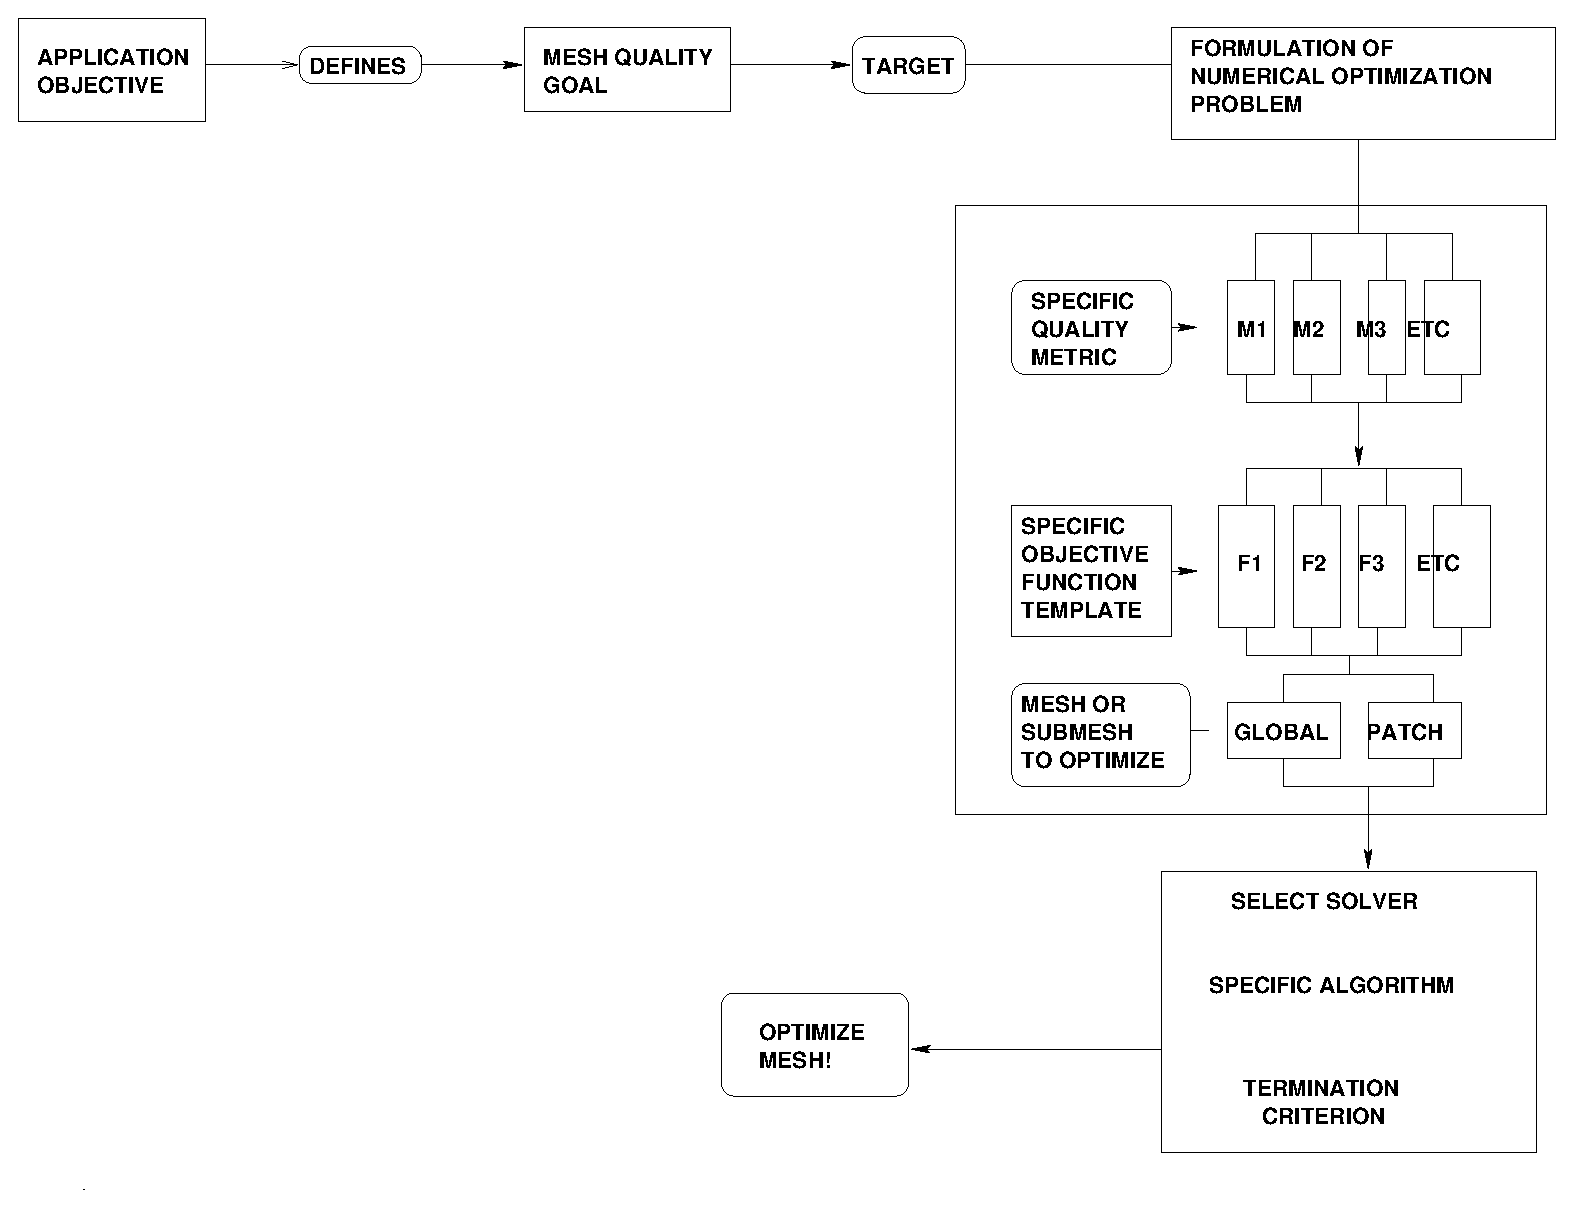
\includegraphics[width=4.7in]{figures/msq-paradigm}
\caption{\em The Mesquite Paradigm \label{Paradigm} }
%\end{tabular}
\end{center}
\end{figure}

\section{How to use this User's Manual}
This user's manual
\begin{itemize}
\item provides an introduction to mesh quality and basic Mesquite concepts (Chapter \ref{sec:intro}),
\item instructs novice users on how to download and install Mesquite (Chapter \ref{sec:install}),
\item provides a tutorial on Mesquite's simplified user's interface and Mesquite's detailed API (Chapter \ref{sec:examples}).
\item describes how to load a mesh in Mesquite via files (Chapter \ref{sec:meshes}), and
%\item provides instructions on using the extensive TSTT interface or a Mesquite mesh specific mesh
%      interface to load a mesh {\it dynamicallu} in Mesquite (sections \ref{sec:msq_mesh}, \ref{sec:TSTT}), and
\item describes Mesquite interactions with domain geometry (Chapter \ref{sec:geom}), and
\item describes Mesquite Wrappers (Chapter \ref{sec:wrappers}),
%\item Exposes in details the concepts and the mechanisms of the advanced API (chapter \ref{sec:API}), and
%\item instructs the user on how to add their own instances of quality
%metrics, objective functions, and solvers (chapter \ref{sec:extensions})
\end{itemize}

Consult the doxygen documentation for the API reference as well as details on the software. There
are two sets of doxygen documentations available:
\begin{itemize}
\item The developer doxygen doc is located in mesquite/doc/developer/. From that directory, you
      must run 'doxygen Mesquite.dox'.
\item The user doxygen doc (API doc) is located in mesquite/doc/user/doxygen. From that directory, you
      must run 'doxygen Mesquite-user.dox'.
\end{itemize}
The doxygen command will generate two directories: an html directory containing the file
index.html that you can open with your web browser, and a latex directory containing a Makefile that
will generate a dvi file.

%\section{Related Documents}

%Documentation of the Mesquite API can be generated from comments in the Mesquite
%source code using the Doxygen utility
%(\url{http://www.stack.nl/~dimitri/doxygen/}).
%To generate HTML and LaTeX copies of this documentation, execute the command
%{\tt doxygen Mesquite-user.dox} in the {\tt doc/usr/doxygen} subdirectory
%of the Mesquite source.

%Further information and related documentation are available on the
%Mesquite home page, located at:
%\url{http://www.cs.sandia.gov/optimization/knupp/Mesquite.html}.

\chapter{UNIFORM GENERATORS}

This chapter contains a description of various uniform generators
already programmed in this library and which were proposed by various 
authors over the past several years, as well as tools for managing
and implementing additional types of generators.
Related generators are regrouped in the same module.
For example, the linear congruential generators (LCGs) are in module
{\tt ulcg}, the multiple recursive generators (MRGs) are in {\tt umrg}, 
the inversive generators in {\tt uinv},
the cubic generators in {\tt ucubic}, etc.
We emphasize that the generators provided here are not all recommendable;
in fact, {\em most of them are not}.

The module {\tt unif01} contains the basic utilities for defining,
manipulating, filtering, combining, and timing generators.  
Each generator must be implemented as an 
object of type {\tt unif01\_Gen}.  To implement one's own generator,
one should create such an object and define all its fields.
For each generator, the structure {\tt unif01\_Gen} must contain a 
function {\tt GetU01} that returns values in the interval $[0,1)$
and a function {\tt GetBits} that returns a block of 32 bits.  
Most of the tests in the {\tt s} modules call the generators
to be tested only indirectly, through the use of the interface 
functions {\tt unif01\_StripD}, {\tt unif01\_StripL} and  
{\tt unif01\_StripB}.
These functions drop the $r$ most significant bits of each random number 
generated and returns a number built out of the remaining bits.

It is also possible to test one's own or an external generator
(that is, a generator that is not predefined in TestU01) very easily with
the help of the functions {\tt unif01\_CreateExternGen01} and
{\tt unif01\_CreateExternGenBits} (see page \pageref{externgen}
of this guide), as long as this generator is programmed in C.

Figure~\ref{fig:usegen} gives simple examples of how to use predefined
generators.  The program creates a LCG with modulus $m = 2^{31}-1$,
multiplier $a = 16807$, and initial state $s = 12345$,
generates and adds 100 uniforms produced by this generator,
prints the sum, and deletes the generator.
To illustrate the fact that there are different ways of getting the
uniforms from the generator, we have generated the first 50 by calling
the {\tt GetU01} function and the next 50 via {\tt unif01\_StripD}.
These two methods are equivalent.
The program then instantiates the generator {\tt lfsr113} available in 
module {\tt ulec}, with the vector $(12345, \ldots, 12345)$ as initial seed,
generates and prints five integers in the range $\{0,\dots,2^{10}-1\}$
(i.e., 10-bit integers) obtained by taking five successive output values
from the generator, stripping out the four most significant bits from 
each value, and retaining the next 10 bits.

For each public identifier used in programs, it is important to
include the corresponding header file before using it,
so as to inform the compiler about the type and signature of functions
and exported variables. For instance, in the following examples, the header
files \texttt{unif01.h}, \texttt{ulcg.h} and \texttt{ulec.h} contain the 
declarations of \texttt{unif01\_Gen}, \texttt{ulcg\_CreateLCG} and 
\texttt{ulec\_Createlfsr113}, respectively.
 
Other examples on how to use the facilities of module {\tt unif01} are given 
at the end of its description.


\setbox0=\vbox {\hsize = 6.0in
\smallc
\verbatiminput{../examples/ex1.c}
}

\begin{figure}
\centering
\myboxit{\box0}
\caption {Using pre-programmed generators\label {fig:usegen}}
\end{figure}


\iffalse  %%%%%%%
%%%%%%%%%%%%%%%%%%%%%%%%%%%%%%%%%%%%%%%%%%%%%%%%%%%%%%%%%%%%%%%

\section {La vitesse des generators}

Les Tableaux \ref{vitesse1}--\ref{vitesse10} donnent une idee 
du temps d'execution moyen
par appel (en micro-secondes), pour un certain number de generators
fournis par the modules {\tt u...}.
Ces values sont en fait le number de secondes
requises pour un million $(10^6)$ d'appels, 
donne ici a une seconde pres.
La machine utilisee etait un SUN UltraSparc 150.
%%  80386 avec coprocesseur 80387, tous deux a 16 MHz.
Pour fins de comparaison, pour un million d'appels a une procedure
``bidon'' ne faisant rien, dans le m\^eme contexte, il a fallu 0.26 secondes.

\begin{table}[htb] \centering \tt
\caption {\rm Vitesse moyenne par appel pour the generators 
          du module ulcg.}
\label {vitesse1}
\begin{tabular}{|l|r|c|l|r|}
\hline
&&&&\\
\multicolumn{1}{|c|}{\rm Generator} & $\mu$-sec. && {\rm Generator}
   & $\mu$-sec.\\
\hline \hline
&&&&\\
 LCG$^1$              &   1.03 && CombLEC2$^2$ &   4.55\\
 LCG$^2$              &   2.33 && CombLEC2$^3$ &  20.22\\
 LCG$^3$              &  10.91 && CombLEC3$^2$ &   6.60\\
 LCGFloat             &   0.80 &&              &  \\
 BigLCG               &  45.24 && CombWH2$^1$  &   2.49\\
 LCG2e31              &   0.98 && CombWH2$^2$  &   4.67\\            
 LCG2e32              &   0.95 && CombWH2$^3$  &  20.40\\            
 LCG2e31m1HD          &   1.73 && CombWH3$^2$  &   7.25\\          
 CombLEC2$^1$         &   2.22 &&              &       \\
&&&&\\
\hline
\end{tabular}

\begin {verse}
 $^1$ : $(m-1)a + c$ representable en {\tt LONGINT} (implantation directe).\\
 $^2$ : implantation utilisee lorsque $a (m\mod a) < m$.\\
 $^3$ : implantation utilisee dans the autres cas.\\
\end {verse}
\end {table}

\begin{table}[htb] \centering \tt
\caption {\rm Vitesse moyenne par appel pour the generators 
              du module umrg.}
\label {vitesse2}
\begin{tabular}{|l|r|c|l|r|}
\hline
&&&&\\
\multicolumn{1}{|c|}{\rm Generator} & $\mu$-sec. && {\rm Generator}
   & $\mu$-sec.\\
\hline \hline
&&&&\\
 MRG$^1$              &  12.36 && MRG$^3$      &   6.35\\
 MRG$^2$              &   4.13 && C2MRG        &  10.71\\
 LagFib               &   0.59 &&              &\\
\hline
\end{tabular}

\begin {verse}
 $^1$ : implantation generale.\\
 $^2$ : implantation plus rapide mentionnee dans {\tt SetMRG}.\\
 $^3$ : varie selon que $p - d < 32$ ou non et que $d < 32$ ou non.\\
\end {verse}
\end {table}


\begin{table}[htb] \centering \tt
\caption {\rm Vitesse moyenne par appel pour the generators du 
              module utaus.}
\label {vitesse3}
\begin{tabular}{|l|r|c|l|r|}
\hline
&&&&\\
\multicolumn{1}{|c|}{\rm Generator} & $\mu$-sec. && {\rm Generator}
   & $\mu$-sec.\\
\hline \hline
&&&&\\
 Taus                 &   0.69 && CombTaus3    &   1.60\\
 TausJ                &   3.52 && Tez95        &   1.48\\
 LongTaus             &   1.07 && TezLec91     &   1.17\\
 CombTaus2            &   1.17 && Tausme3a     &   1.49\\
&&&&\\
\hline
\end{tabular}

\end {table}

\begin{table}[htb] \centering \tt
\caption {\rm Vitesse moyenne par appel pour the generators 
              du module ugfsr.}
\label {vitesse4}
\begin{tabular}{|l|r|c|l|r|}
\hline
&&&&\\
\multicolumn{1}{|c|}{\rm Generator} & $\mu$-sec. && {\rm Generator}
   & $\mu$-sec.\\
\hline \hline
&&&&\\
 GFSR                 &   0.66 && Toot73       &   0.62\\
 TGFSR                &   0.81 && Fushimi90    &   0.67\\
 Ripley90             &   0.53 && Kirk81       &   0.65\\
&&&&\\
\hline
\end{tabular}

\end {table}

\begin{table}[htb] \centering \tt
\caption {\rm Vitesse moyenne par appel pour the generators 
              du module uinv.}
\label {vitesse5}
\begin{tabular}{|l|r|c|l|r|}
\hline
&&&&\\
\multicolumn{1}{|c|}{\rm Generator} & $\mu$-sec. && {\rm Generator}
   & $\mu$-sec.\\
\hline \hline
&&&&\\
 InvImpl              &  14.18 && InvExpl      &  14.77\\
 InvImpl2a            &  22.95 && InvExpl2a    &  35.21\\
 InvImpl2b            &  22.82 && InvExpl2b    &  27.46\\
 InvMRG               &  23.12 &&              &       \\
&&&&\\
\hline
\end{tabular}

\end {table}

\begin{table}[htb] \centering \tt
\caption {\rm Vitesse moyenne par appel pour the generators 
              du module uquad.}
\label {vitesse6}
\begin{tabular}{|l|r|c|l|r|}
\hline
&&&&\\
\multicolumn{1}{|c|}{\rm Generator} & $\mu$-sec. && {\rm Generator}
   & $\mu$-sec.\\
\hline \hline
&&&&\\
 Quadratic            &  13.81 && Quadratic2$^1$&  14.77\\
 Quadratic2           &   1.63 &&               &       \\
&&&&\\
\hline
\end{tabular}

\begin {verse}
$^1$ : implantation rapide : e = 32.\\
\end {verse}
\end {table}

\begin{table}[htb] \centering \tt
\caption {\rm Vitesse moyenne par appel pour the generators 
              du module ulec.}
\label {vitesse7}
\begin{tabular}{|l|r|c|l|r|}
\hline
&&&&\\
\multicolumn{1}{|c|}{\rm Generator} & $\mu$-sec. && {\rm Generator}
   & $\mu$-sec.\\
\hline \hline
&&&&\\
 CombLec88            &   2.98 && CombMRG96       &   5.47\\
 MRG93                &   3.31 && CombMRG96d      &  11.22\\
 CombLec88Float       &   1.38 && CombMRG96Float  &   2.60\\
                      &        && CombMRG96dFloat &   5.13\\
&&&&\\
\hline
\end{tabular}

\end {table}

\begin{table}[htb] \centering \tt
\caption {\rm Vitesse moyenne par appel pour the generators 
              du module ucarry.}
\label {vitesse8a}
\begin{tabular}{|l|r|c|l|r|}
\hline
&&&&\\
\multicolumn{1}{|c|}{\rm Generator} & $\mu$-sec. && {\rm Generator}
   & $\mu$-sec.\\
\hline \hline
&&&&\\
 AWC                  &   0.85 && MWC$^1$      &  13.03\\
 SWC                  &   0.85 && SWC$^1$      &   3.79\\
&&&&\\
\hline
\end{tabular}

\begin {verse} 
 $^1$ : implantation generale, e = 32.\\
\end {verse} 
\end {table}

\begin{table}[htb] \centering \tt
\caption {\rm Vitesse moyenne par appel pour the generators 
              du module umarsa.}
\label {vitesse8}
\begin{tabular}{|l|r|c|l|r|}
\hline
&&&&\\
\multicolumn{1}{|c|}{\rm Generator} & $\mu$-sec. && {\rm Generator}
   & $\mu$-sec.\\
\hline \hline
&&&&\\
 KISS                 &   0.76 && Combo        &   1.15\\
 Marsa90a             &   0.87 && ECG1         &   1.34\\
 Marsa90b             &   0.83 && ECG2         &   1.31\\
 Mother0              &   1.77 && ECG3         &   1.39\\
                       &&& ECG4                &   1.36 \\
% Mother1$^1$          &   5.95 &&              &       \\
&&&&\\
\hline
\end{tabular}
\end {table}

\begin{table}[htb] \centering \tt
\caption {\rm Vitesse moyenne par appel pour the generators 
              du module unumrec.}
\label {vitesse9}
\begin{tabular}{|l|r|c|l|r|}
\hline
&&&&\\
\multicolumn{1}{|c|}{\rm Generator} & $\mu$-sec. && {\rm Generator}
   & $\mu$-sec.\\
\hline \hline
&&&&\\
 Setran0              &   2.33 &&  Setran2      &   5.25\\
 Setran1              &   2.91 &&               &       \\
&&&&\\
\hline
\end{tabular}

\end {table}

\begin{table}[htb] \centering \tt
\caption {\rm Vitesse moyenne par appel pour the generators 
              des modules uvaria et ufile.}
\label {vitesse10}
\begin{tabular}{|l|r|c|l|r|}
\hline
&&&&\\
\multicolumn{1}{|c|}{\rm Generator} & $\mu$-sec. && {\rm Generator}
   & $\mu$-sec.\\
\hline \hline
&&&&\\
 Tindo                &  64.31 && ACORN        &  75.33\\
 CSD                  &   6.03 && ReadFile     &  13.82\\
&&&&\\
\hline
\end{tabular}

\end {table}

\fi   %%%%%%%%%%%%%%%%%%%%

\defmodule {unif01}

This module offers basic tools for defining, manipulating, and
transforming uniform random number generators to which tests are 
to be applied or which could be used for other purposes.
Each generator is implemented as a
structure of type {\tt unif01\_Gen}. 
Several predefined generators are available in the {\tt u} modules.
Each such generator must be created by the appropriate 
{\tt \ldots Create\ldots} function before being used, and should
be deleted by the corresponding {\tt \ldots Delete\ldots} function
to free the memory used by the generator when it is no longer needed.
One can create and use simultaneously any number of generators. 
These generators are usually passed to functions as pointers to
objects of type {\tt unif01\_Gen}.

One may call an external generator for testing using the functions in
this module. See Figure~\ref{prog:ex7} for an example.
One may also implement one's own generator, by creating a structure of 
type {\tt unif01\_Gen} and defining all its fields properly.
See Figure~\ref{fig:my16807} for an illustration.

Each implemented generator returns either a floating-point 
number in $[0, 1)$ (via its function {\tt GetU01}) 
or a block of 32 bits (via its function {\tt GetBits}).
Ideally, these should follow the uniform distribution $(0,1)$
and $\{0,\dots,2^{32}-1\}$, respectively.
Most of the tests in the {\tt s} modules actually call the generator
to be tested only indirectly through the use of one of the interface 
functions {\tt unif01\_StripD},
 {\tt unif01\_StripL} and  {\tt unif01\_StripB}.
These functions drop the $r$ most significant bits of each random number 
and return a number built out of the remaining bits.

Functions are also provided for adding one or many output {\em filters\/} 
to a given generator. These functions create another generator
object which implements a mechanism that automatically
transforms the output values of the original generator in a specified way.
One can also combine the outputs of several generators in different ways.
By using the output of several generators or several substreams of the
same generator in a round-robin way, one can test the quality of these as 
examples of parallel generators.
Finally, tools are provided for measuring the speed of generators
and adding their output values (for testing purposes).



%%%%%%%%%%%%%
\bigskip\hrule
\code\hide
/*  unif01.h  for ANSI C  */
#ifndef UNIF01_H
#define UNIF01_H
\endhide
#include "gdef.h"
\endcode


%%%%%%%%%%%%%%%%%%%%%%%%%%%%%%%%%%%%%%%%%%
\guisec{Basic types}
\code

typedef struct {
   void *state;
   void *param;
   char *name;
   double (*GetU01) (void *param, void *state);
   unsigned long (*GetBits) (void *param, void *state);
   void (*Write) (void *state);
} unif01_Gen;
\endcode
  \tab Generic random number generator. The function {\tt GetU01}
   returns a floating-point number in $[0,1)$ while {\tt GetBits}
   returns a block of 32 bits. If the generator delivers less than 32
   bits, these bits are left shifted so that the most
   significant bits are the relevant ones.
% If the generator returns less than 32 bits of precision, then one must make
% sure that these bits are the most significant bits of the returned block.
   The variable {\tt state} keeps the
   current state of the generator and {\tt param} is the set of
   specific parameters used in computing the next random number. 
   The function  {\tt Write} will write the current state of the
   generator. The string  {\tt name}  describes the current generator,
   its parameters, and its initial state.
   In the description of the generators in the u modules, one
   indicates how the {\tt GetU01} function  gets its value from the
   generator's recurrence;
   it is always understood that the {\tt GetBits}  function is
   equivalent to $2^{32}\,${\tt GetU01}.
  \endtab

%%%%%%%%%%%%%%%%%%%%%%%%%%%%%%%%%%%%%%%%%%
\guisec{Environment variables}

\ifdetailed
\code

#define unif01_MASK32  0xffffffffUL
\endcode
  \tab 32-bit mask.
 \endtab
\code


#define unif01_NORM32  4294967296.0
#define unif01_INV32   2.328306436538696289e-10
\endcode 
 \tab The constants $2^{32}$ and $1/2^{32}$ respectively: 
   normalization factors used in many generators to transform
  a floating-point ``random'' number into a 32-bit integer, or vice-versa.
 \endtab
\fi

\code


extern lebool unif01_WrLongStateFlag;
\endcode
  \tab For generators whose state is a large array, determines whether
   the state will be written out in full ({\tt TRUE}) or not ({\tt FALSE})
   in the printouts. The default value is {\tt FALSE}. 
\hrichard{C'est la seule variable globale qui reste. On pourrait
  l'\'eliminer en ajoutant un argument \`a unif01\_Gen.Write, qui
  deviendrait  {\tt Write (void *state, lebool flag).}}
 \endtab



%%%%%%%%%%%%%%%%%%%%%%%%%%%%%%%%%%%%%%%%%%
\guisec{Basic functions}

\code


double unif01_StripD (unif01_Gen *gen, int r);
\endcode
\tab Makes one call to the generator {\tt gen}, drops the $r$ most
  significant bits, left-shift the others by $r$ positions, and
  returns the result, which is a floating-point number in $[0,1)$.
 More specifically, returns $2^r u \mod 1$, 
 where $u$ is the output of {\tt gen}.
 \endtab
\code


long unif01_StripL (unif01_Gen *gen, int r, long d);
\endcode
\tab
 Similar to {\tt unif01\_StripD}, but generates an integer ``uniformly'' over
 the set $\{0,\dots,d-1\}$, by using the most significant bits of the
 output of {\tt gen} after having dropped the first $r$ bits.
 More specifically, returns $\lfloor d (2^r u \mod 1)\rfloor$, 
 where $u$ is the output of {\tt gen}.
\endtab
\code


unsigned long unif01_StripB (unif01_Gen *gen, int r, int s);
\endcode
\tab
 Calls the generator {\tt gen}, drops the $r$ most significant bits,
 and returns the $s$ following bits as an integer in 
 the set $\{0,\dots,2^s-1\}$.
\endtab
\code


void unif01_WriteNameGen (unif01_Gen *gen);
\endcode
 \tab  Writes the character string {\tt gen->name} that describes the
  generator.
 \endtab
\code


void unif01_WriteState (unif01_Gen *gen);
\endcode
 \tab  Writes the current state of generator  {\tt gen}.
 \endtab
\code


void unif01_WrLongStateDef (void);
\endcode
 \tab Dummy function used when the state of the current
   generator is a large array and we do not want to write the full state.
   Writes the message ``{\tt   Not shown here ... takes too much space}''.
 \endtab
\code


unif01_Gen * unif01_CreateDummyGen (void);
\endcode
\tab  Creates a {\em dummy\/} generator, which does nothing and always
\index{Generator!dummy}%
  returns zero. It can be used for instance to measure the overhead of
  function calls when comparing generator's speeds
  (see the timing tools below).
\endtab
\code


void unif01_DeleteDummyGen (unif01_Gen *gen);
\endcode
\tab  Frees the dynamic memory used by the dummy generator above.
\endtab
\ifdetailed
\code


void unif01_DeleteGen (unif01_Gen *gen); 
\endcode 
\tab  Frees the dynamic memory used by a typical generator, for which
  the state does not contain dynamically allocated arrays. 
  In this case, the memory
  is allocated by a {\tt u\ldots\_Create\ldots} function in some
  {\tt u} module and the present function is called by the corresponding
  {\tt u\ldots\_Delete\ldots} function in the same {\tt u} module.
\endtab
\fi



%%%%%%%%%%%%%%%%%%%%%%%%%%%%%%%%%%%%%%%%%%
\guisec{Output filters}

The following describes some filters that can be added to transform 
the output of a given generator. In each case, a new generator object is
created that will effectively apply the filter to the original generator.
One may apply more than one filter at a time on a given generator
(for example, one may apply the {\tt Double}, the  {\tt Bias}, the 
 {\tt Trunc} and the {\tt Lac} filters on top of one another). It suffices
 to create the appropriate filters as described below.  The resulting 
filtered generator(s) will call the original generator behind the scenes.
Thus the state of the original generator will evolve as usual, even
though it is not called directly.\index{filters}


The different filters applied on an original generator are not independent
but are related as the elements of a stack. When they are no longer in use, 
they must be deleted {\em in the reverse order of their creation}, 
the original generator being the last one of this group to be deleted. 
Figure~\ref{fig:prog-filter} illustrates how these facilities can be used.

\code


unif01_Gen * unif01_CreateDoubleGen (unif01_Gen *gen, int s);
\endcode
 \tab
 Given a generator {\tt gen}, this function
\index{Generator!filter!increased precision}%
 creates and returns a generator with increased precision, such that
 every call to this new generator
 corresponds to two successive calls  to the original generator.
 The method {\tt GetU01} of this doubled generator  returns
 $(U_1 +  U_2/2^s)$ mod 1, where $U_1$ and $U_2$ are the results of
 two successive calls  to the method {\tt GetU01} of {\tt gen}. 
 If the current generator has 31 bits of precision, for example,
 then one can obtain 53 bits of precision from {\tt GetU01} 
 by creating this new generator with {\tt s}  between $22$ and $31$.
% Not true anymore:
%  The function {\tt GetBits} of this new generator 
%  will return  $(X_1 +  X_2/2^s)$ mod $2^{32}$,
%  where $X_1$ and $X_2$ are the results of two successive calls to  the
%  method  {\tt GetBits} of the original {\tt gen}.
%  So it may return  more bits of precision, but never more than 32 bits.  
 \endtab
\code


unif01_Gen * unif01_CreateDoubleGen2 (unif01_Gen *gen, double h);
\endcode
 \tab A more general version of {\tt unif01\_CreateDoubleGen} where
  the method {\tt GetU01} of the double generator  returns
  $(U_1 +  h U_2)$ mod 1. Restriction: $0 < h < 1$.
 \endtab
\code


unif01_Gen * unif01_CreateLacGen (unif01_Gen *gen, int k, long I[]);
\endcode
 \tab
  Given an original generator {\tt gen}, this function 
\index{Generator!filter!lacunary indices}%
  creates and returns a generator involving lacunary indices, such that
  successive calls to this new generator
  will no longer provide successive values from the original
  generator, but rather selected values as specified by
  the table {\tt I[0..k-1]}, in a circular fashion.
  More specifically, if $u_0, u_1, u_2, \dots$ is the sequence
  produced by the original {\tt gen}, if the table {\tt I[0..k-1]}
  contains the non-negative integers $i_0, \dots i_{k-1}$ (in increasing
  order), and if we put $L = i_{k-1}+1$,
  then the output sequence of the new generator will be:
   $$ u_{i_0}, u_{i_1}, \dots, u_{i_{k-1}}, u_{L+i_0}, u_{L+i_1},
      \dots, u_{L+i_{k-1}}, u_{2L+i_0}, u_{2L+i_1}, \dots. $$
  For example, if  $k=3$ and $I = \{0, 3, 5\}$,
  the output sequence will be the numbers
   $$ u_{0}, u_{3}, u_{5}, u_{6}, u_{9}, u_{11}, u_{12}, \dots $$
  of the original generator.
  To obtain every $s$-th number produced by the original generator
  for example (a {\em decimated sequence\/}), one should take
  $k=1$ and $I = \{s-1\}$.
%  (note that taking $I = \{0, s\}$ won't work; it would return
%  $u_0, u_s, u_{s+1}, u_{2s+1}, \dots$).
 \endtab
\code


unif01_Gen * unif01_CreateLuxGen (unif01_Gen *gen, int k, int L);
\endcode
 \tab   Given an original generator {\tt gen}, this function
\index{Generator!filter!luxury}% 
  creates and returns a new generator giving the output of the
  original generator with luxury level $L$: out of every group of $L$
  random numbers, the first $k$ are kept and the next $L-k$ are skipped.
 \endtab
\code


unif01_Gen * unif01_CreateBiasGen (unif01_Gen *gen, double a, double p);
\endcode
 \tab  Given an original generator {\tt gen}, this function 
  creates and returns a new generator giving a biased output of the
  original generator.  The output is biased 
\index{Generator!filter!biased output}%
  in such a way that the density becomes
  constant with total probability $p$ over the interval $[0, a)$, and
  constant with total probability $1 - p$ over $[a, 1)$ (the two constant
  densities are different). For example, by choosing $p= 1$ and $a = 0.5$,
  all the random numbers generated by {\tt GetU01} will fall
  on the interval $[0,\; 0.5)$. This filter can be used, for example,
  to study the power of certain statistical tests.
  Restrictions: $0 < a < 1$ and $0 \le p \le 1$.
 \endtab
\code


unif01_Gen * unif01_CreateTruncGen (unif01_Gen *gen, int s);
\endcode
 \tab   Given an original generator {\tt gen}, this function
\index{Generator!filter!bit truncated}% 
  creates and returns a new generator giving the output of the
  original generator truncated to its $s$ most significant bits.
 Restriction: $s \le 32$.
\endtab
\code


unif01_Gen * unif01_CreateBitBlockGen (unif01_Gen *gen, int r, int s,
                                       int w);
\endcode
 \tab  Consider a group of $v \le 32$ successive 32-bit integers
  outputted by generator {\tt gen}. For each of these, drop the $r$ most
\index{Generator!filter!blocks of bits}% 
  significant bits and keep the $s$ following bits numbered
  $b_{i 1}, b_{i 2}, \ldots, b_{i s}$, starting with the
  most significant, for $1 \le i \le v$.
  Make with all these a $v\times s$ matrix of bits, say ${\cal B}$.
  The generator returned by this function is a filter that builds new 32-bit
   integers from $v\times w$ submatrices of ${\cal B}$. 
  The number of columns of the submatrix $w$ must be a power of 2 no larger
  than 32 and it must be $\le s$. If $w$ does not divide $s$ exactly,
  the last submatrix of ${\cal B}$ will have less than $w$ columns and
  will be disregarded.

  If the stream of bits thus obtained from {\tt gen} is
  $$
   b_{1 1}, b_{1 2}, \ldots,  b_{1 s},
   b_{2 1}, b_{2 2}, \ldots,  b_{2 s},
   \ldots,
   b_{v 1}, b_{v 2}, \ldots,  b_{v s}, \ldots
$$
   then the new integers returned by the filter will be 32-bit integers
   taken from the rearranged stream of bits so that the first new 
   number is (its most significant bit being given first)
  $$
   b_{1 1}, b_{1 2}, \ldots,  b_{1 w},
   b_{2 1}, b_{2 2}, \ldots,  b_{2 w},
   \ldots,
   b_{v 1}, b_{v 2}, \ldots,  b_{v w},
$$
  the second new  number is made of the bits (its most
  significant bit first)
  $$
   b_{1 (w+1)}, b_{1 (w+2)}, \ldots,  b_{1 (2w)},
   b_{2 (w+1)}, b_{2 (w+2)}, \ldots,  b_{2 (2w)},
   \ldots,
   b_{v (w+1)}, b_{v (w+2)}, \ldots,  b_{v (2w)},
  $$
  and so on.

  The following examples illustrates how the filter works.
  If $r$ = 0 and $w = s = 32$, then the filter has no effect,
  the new integers being the same as those outputted by  {\tt gen}.
  If $r$ = 0 and $w = s = 1$, then the filter will return integers
  made only from the most significant bit of the original integers, all 
  other bits being dropped.
  If $r$ = 0, $w = 1$ and $ s = 32$, then the filter will return integers
  made from the columns of ${\cal B}$, i.e., since the rows of ${\cal B}$
  are made of the original integers, the filter will return the columns
  of ${\cal B}$ as the new integers. 
  Restrictions: $r \ge 0$, $0 < s \le 32$ and
   $w$ in  $\{1, 2, 4, 8, 16, 32\}$.
 \endtab
\code


void unif01_DeleteDoubleGen (unif01_Gen *gen);
void unif01_DeleteLacGen    (unif01_Gen *gen);
void unif01_DeleteLuxGen    (unif01_Gen *gen);
void unif01_DeleteBiasGen   (unif01_Gen *gen);
void unif01_DeleteTruncGen  (unif01_Gen *gen);
void unif01_DeleteBitBlockGen (unif01_Gen *gen);
\endcode
 \tab Frees the memory used by the generator created by the corresponding
 {\tt Create} functions above.
 \endtab



%%%%%%%%%%%%%%%%%%%%%%%%%%
\guisec{Combining generators}

These functions permit one to define the combination of two, three 
or more generators. The resulting generator calls
\index{Generator!combined}\index{combined generators}% 
the component generators behind the scenes, so it changes their
state. \emph{The  component generators must not be destroyed as long as the
 combination generator is in use.}
One can obtain the combinations of more than three generators by combining
the generators obtained from combinations of two or three generators.
%
\hide
\code

typedef struct {
   unif01_Gen *gen1;
   unif01_Gen *gen2;
} unif01_Comb2_Param;
\endcode 
 \tab This is used for combining two arbitrary generators. It is made
  public because it would not be possible otherwise to free the dynamic
  memory used by the two component generators when they are programmed
  in another module.
  \endtab
\endhide
\code


unif01_Gen * unif01_CreateCombAdd2 (unif01_Gen *gen1, unif01_Gen *gen2,
                                    char *name);
\endcode
 \tab  This function creates and returns a generator whose output is the
 addition of the outputs modulo 1 of the  method {\tt GetU01} of the 
 two generators {\tt gen1} and {\tt gen2}.
 The character string {\tt name} may be printed in reports to identify this
 new combined  generator.
\index{combined generators!addition}
 \endtab
\code


unif01_Gen * unif01_CreateCombAdd3 (unif01_Gen *gen1, unif01_Gen *gen2,
                                    unif01_Gen *gen3, char *name);
\endcode
 \tab  Same as {\tt unif01\_CreateCombAdd2}, except that the returned
  generator is the combination (the addition of the outputs modulo 1 of the
  method {\tt GetU01}) of the three generators {\tt gen1, gen2} and {\tt gen3}.
\hrichard{
  When the combined generator is used to generate random integers, in rare
  cases, an integer may differ by 1 unit depending on the order of
   addition of the 3 terms (one from each component). This is due
   to the last bit (bit 53) of the value returned which may be affected by
   floating-point numerical errors. Furthermore, the result
   may be different if the addition is done without function calls
   (as in the pre-programmed version of Wichmann-Hill for example in
   {\tt ulcg\_CreateCombWH3}), in  which
   case, the 2 extra guard bits required by the IEEE-754 standard in
   floating-point arithmetic operations may give a more exact result.
}
 \endtab
\code


unif01_Gen * unif01_CreateCombXor2 (unif01_Gen *gen1, unif01_Gen *gen2,
                                    char *name);
\endcode
 \tab  This function creates and returns a generator whose output is the
 bitwise {\sl exclusive-or (XOR)\/}  of the outputs of the two generators
 {\tt gen1} and {\tt gen2}. The character string {\tt name} may be printed
 in reports to identify this combined generator.
 \index{combined generators!exclusive or}
 \endtab
\code


unif01_Gen * unif01_CreateCombXor3 (unif01_Gen *gen1, unif01_Gen *gen2,
                                    unif01_Gen *gen3, char *name);
\endcode
 \tab  Same as {\tt unif01\_CreateCombXor2}, except that the 
 returned generator is the combination of the three generators
 {\tt gen1, gen2} and {\tt gen3}.
 \endtab
\code


void unif01_DeleteCombGen (unif01_Gen *gen);
\endcode
 \tab  Frees the memory used by one of the combination generators returned
  by the  {\tt Create} functions above, but does not delete any of its
  component generators.
 \endtab


%%%%%%%%%%%%%%%%%%%%%%%%%%
\guisec{Parallel generators}

 The following functions allow the joining of the output of several generators
 or of different substreams of the same generator into a single stream of
 random numbers. This can be used to test for apparent correlations between the
 output of several generators or several substreams used in parallel.
 For example, one may want to choose seeds 
 that are far separated for the same generator, while making sure that 
 such seed choice is statistically valid and does not introduce unwanted 
 correlation between the substreams thus defined.
\code

unif01_Gen * unif01_CreateParallelGen (int k, unif01_Gen *gen[], int L);
\endcode
 \tab Creates and returns a generator whose output is obtained in a round-robin
  way $L$ numbers at a time from each of the $k$ generators \texttt{gen[i]} as 
  follows: the first $L$ numbers are generated from \texttt{gen[0]}, the next 
  $L$ numbers are generated from \texttt{gen[1]}, and so on until 
  $L$ numbers have been generated from \texttt{gen[k-1]}, after which, this whole
  process is repeated. \emph{It is important that none of the generators} 
 \texttt{gen[i]} \emph{be destroyed as long as the parallel generator is in use.}
 \endtab
\code


void unif01_DeleteParallelGen (unif01_Gen *gen);
\endcode
 \tab  Frees the memory allocated by the parallel generator returned
  by the  {\tt Create} function above, but \emph{does not} delete any of its
  component generators, which is the responsibility of the program that
  created them.
 \endtab


%%%%%%%%%%%%%%%%%%%%%%%%%%
\guisec{External generators}

Although  TestU01 implements many generators both in generic and in
specific forms, it is not possible to implement all those that are in
existence because there are just too many and new ones are proposed 
regularly. The typical user would like to test his preferred generator
with as little complications as possible. The functions below allows one 
to do just that. As long as the generator is programmed in C, 
one has but to pass  the function implementing the generator to one of the
functions below and call some of the tests available in TestU01.
It is the responsibility of the user to ensure that his generator does not
violate the conditions described in the functions below. For the
call in {\tt unif01\_CreateExternGen01}, his generator must return
floating-point numbers in $[0, 1)$. For the calls in
 {\tt unif01\_CreateExternGenBitsL} and  {\tt unif01\_CreateExternGenBits},
 his generator must return an integer in the interval $[0, 2^{32} - 1]$.
If these conditions are violated, the results of the tests in TestU01 are
unpredictable. % Similarly, a generator should not be so pathological so as to
% return the same value at every call. 
 \index{Generator!user defined} \index{Generator!external}%
\code


unif01_Gen *unif01_CreateExternGen01 (char *name, double (*gen01)(void*,void*),
                                      unsigned long (*gen01_bits)(void*,void*));
\endcode
\tab Implements a pre-existing external generator {\tt gen01} that is
  not part of TestU01. \label{externgen}
 It must be a C function taking no argument and returning a {\tt double}
 in the interval $[0, 1)$. Parameter {\tt name} is the name of the generator.
 No more than one generator of this type can be in use at a  time. 
\endtab
\code


unif01_Gen *unif01_CreateExternGenBits (char *name,
                                        unsigned int (*genB)(void));
\endcode
\tab Implements a pre-existing external generator {\tt genB} that is not part
 of TestU01. It must be a C function taking no argument and returning
 an integer in the interval $[0, 2^{32} - 1]$.
 If the generator delivers less than 32 bits of resolution, then these 
 bits must be left shifted so that the most significant bit is bit 31
 (counting from 0). Parameter {\tt name} is the name of the generator.
 No more than one generator of this type can be in use at a  time. 
 \endtab
\code


unif01_Gen *unif01_CreateExternGenBitsL (char *name,
                                         unsigned long (*genB)(void));
\endcode
\tab Similar to {\tt unif01\_CreateExternGenBits}, but with
{\tt unsigned long} instead of {\tt unsigned int}. The generator 
{\tt genB} must also return  an integer in the interval $[0, 2^{32} - 1]$.
 \endtab
\code


void unif01_DeleteExternGen01 (unif01_Gen * gen);
void unif01_DeleteExternGenBits (unif01_Gen * gen);
void unif01_DeleteExternGenBitsL (unif01_Gen * gen);
\endcode
 \tab  Frees the memory used by the generator created by the corresponding
 {\tt Create} functions above.
 \endtab


\bigskip
As an example, Figure~\ref{prog:ex7}  shows how to apply
 {\tt SmallCrush}, a small predefined battery of tests (described on page
 \pageref{bat:SmallCrush}) to the generators {\tt MRG32k3a} and {\tt
xorshift}, whose code is shown in Figures~\ref{fig:MRG32k3a} and
 \ref{fig:xorshift}.  One must compile and link the two external
files with the main program and the TestU01 library.
The generator {\tt MRG32k3a} returns numbers in (0, 1) and was
proposed by L'Ecuyer in \cite{rLEC99b}.
The generator {\tt xorshift} returns 32-bit integers 
and was proposed by Marsaglia in \cite[page 4]{rMAR03a}.


%%%%%%%%%%%%%%%%%%%%%%%%%%%%%%%%%%%%%%%%%%%%%%

\setbox0=\vbox {\hsize = 6.2in
{\smallc
\verbatiminput{../examples/ex7.c}}
}

\begin{figure} \centering \myboxit{\box0}
\caption {Example of a program to test two external generators}
\label {prog:ex7}
\end{figure}


\setbox1=\vbox {\hsize = 6.2in
{\smallc
\verbatiminput{../examples/mrg32k3a.c}}
}

\begin{figure} \centering \myboxit{\box1}
\caption {External function for {\tt MRG32k3a}.}
\label {fig:MRG32k3a}
\end{figure}


\setbox1=\vbox {\hsize = 6.2in
{\smallc
\verbatiminput{../examples/xorshift.c}}
}

\begin{figure} \centering \myboxit{\box1}
\caption {External function for {\tt xorshift}.}
\label {fig:xorshift}
\end{figure}


%%%%%%%%%%%%%%%%%%%%%%%%%%%%%%%%%%%%%%%%%%%%%%
\guisec{Timing devices}

\code

typedef struct {
   unif01_Gen *gen;
   long n;
   double time;
   double mean;
   lebool fU01;
   } unif01_TimerRec;
\endcode
 \tab  Structure to memorize the results of speed and sum tests on a given
   generator. Here, {\tt gen} is the generator,\index{timer}
   {\tt n} is the number of calls made to the generator,
   {\tt time} is the total CPU time in seconds, and
   {\tt mean} is the mean of the {\tt n} output values of the generator.
   If {\tt fU01} is  {\tt TRUE}, the function {\tt GetU01} of 
   {\tt gen} is called, otherwise the function  {\tt GetBits} is called.
 \endtab
\code


void unif01_TimerGen (unif01_Gen *gen, unif01_TimerRec *timer, long n,
                      lebool fU01);
\endcode
 \tab
 This function computes the CPU time needed to generate
\index{Generator!speed}\index{Generator!timing}%
  {\tt n} random numbers with the generator {\tt gen},
  and returns the result in {\tt timer}. If {\tt fU01} is  {\tt TRUE},
  the random numbers will be generated by the method {\tt GetU01} of 
  {\tt gen}, otherwise by the
  method  {\tt GetBits}.
 \endtab
\code


void unif01_TimerSumGen (unif01_Gen *gen, unif01_TimerRec *timer, long n,
                         lebool fU01);
\endcode
 \tab
  Same as {\tt unif01\_TimerGen}, but also adds the {\tt n} random
  numbers and saves their mean in {\tt timer->mean}.
 \endtab
\code


void unif01_WriteTimerRec (unif01_TimerRec *timer);
\endcode
 \tab
  Prints the results contained in {\tt timer}, with some information
  about the generator and the current machine. One should make sure that the
  generator {\tt gen} in {\tt timer} has not been deleted when
  calling this function. 
\hrichard {Ceci m'inqui\`ete un peu, car si
l'utilisateur appelle cette fonction apr\`es que le g\'en\'erateur 
ait \'et\'e d\'etruit, il y aura un {\tt segmentation fault}. L'alternative
serait de r\'eserver un tableau de 50 caract\`eres dans 
{\tt unif01\_TimerRec} et d'y recopier le nom du g\'en\'erateur, au lieu
d'avoir le pointeur {\tt gen}.}
 \endtab
\code


void unif01_TimerGenWr (unif01_Gen *gen, long n, lebool fU01);
\endcode
 \tab
  Equivalent to calling {\tt unif\_TimerGen} followed by 
  {\tt unif01\_WriteTimerRec}. 
 \endtab
\code


void unif01_TimerSumGenWr (unif01_Gen *gen, long n, lebool fU01);
\endcode
 \tab
  Equivalent to calling {\tt unif\_TimerSumGen} followed by 
  {\tt unif01\_WriteTimerRec}. 
 \endtab
\code
\hide
#endif
\endhide
\endcode

%%%%%%%%%%%%%%%%%%%%%%%%%%%%%%%%%%%%%%%%%%%%%%%%%%%%%%%%%%%%%

\subsection*{Examples}

We now provide some examples of how to use the facilities of {\tt unif01}.
Figure~\ref{fig:my16807} gives an example of how to implement one's own
generator, using all the paraphernalia of TestU01. This is specially
useful when one wants to implement a generator in generic form with
one or more parameters.
 This is a simple LCG with hardcoded parameters $m=2^{31}-1$ 
and $a = 16807$.\index{Generator!user defined}
The function {\tt My16807\_U01} will advance the generator's state
by one step and return a $U(0,1)$ random number $U$ each time it is
called, whereas {\tt My16807\_Bits} will return the 32 most significant
bits in the binary representation of $U$.
The function {\tt CreateMy16807} allocates the memory for the corresponding
{\tt unif01\_Gen} structure and initializes all its fields.


\setbox2=\vbox {\hsize = 6.2in
{\smallc
\verbatiminput{../examples/my16807.c}}
}

\begin{figure} \centering \myboxit{\box2}
\caption {A user-defined generator, in file {\tt my16807.c}.}
\label {fig:my16807}
\end{figure}


%%%%%%%%%%%%%%%%%%%%%%%%%%%%%%%%%%%%%%%%%%%%%

Figure~\ref{fig:unif-timing} shows how to use the timing facilities.
The {\tt main} program first sets the generator {\tt gen} to an LCG
with modulus $2^{31}-1$, multiplier $a = 16807$, and initial state 12345,
implemented in floating point. 
\hrichard {Sur ma machine Linux, le
   LCG (en entiers) est 12\% plus rapide que la version LCGFloat} 
(This generator is well known, but certainly {\em not\/} to be recommended;
its period length of $2^{31}-2$ is much too small.)
The program calls {\tt unif01\_TimerSumGenWr} which generates 10 million 
random numbers in $[0, 1)$, computes their mean, and prints the CPU time 
needed to do that.
Next, the program deletes this {\tt unif01\_Gen} object and creates a 
new one, which is actually a user-defined implementation of the same LCG,
taken from the home-made module {\tt my16807} whose code is shown in
Figure~\ref{fig:my16807}.
In this implementation, the parameters have been placed as constants 
directly into the code.
Ten million random numbers are generated with this alternative 
implementation, and the average and CPU time are printed.
The same procedure is repeated for two additional predefined
generators taken from modules {\tt ulec}.
% with period lengths near $2^{191}$ and near $2^{113}$, respectively. 
Figure~\ref{fig:unif-timing-res} shows the results of this program,
run on a 2106 MHz computer running Linux, and compiled with {\tt gcc -O2}.


%%%%%%%%%%%%%%%%%%%%%%%%%%%%%%%%%%%%%%%%%%%%%%

\setbox0=\vbox {\hsize = 6.2in
{\smallc
\verbatiminput{../examples/ex3.c}}
}

\begin{figure} \centering \myboxit{\box0}
\caption {Example of a program creating and timing generators.}
\label {fig:unif-timing}
\end{figure}


\setbox1=\vbox {\hsize = 6.2in
{\smallc
\verbatiminput{../examples/ex3.res}}
}

\begin{figure} \centering \myboxit{\box1}
\caption {Results of the program of Figure~\ref{fig:unif-timing}.}
\label {fig:unif-timing-res}
\end{figure}


%%%%%%%%%%%%%%%%%%%%%%%%%%%%%%%%%%%%%%%%%%%%%

Figure~\ref{fig:prog-filter} shows how to apply filters to generators
and how to combine two or more generators by addition modulo 1 or bitwise
exclusive-or.
The program starts by creating a simple Tausworthe generator {\tt gen1}
and it generates 20 values from it.
It then deletes {\tt gen1}, creates a new copy of it with the same 
parameters and initial state, and applies a ``lacunary indices'' 
filter to create a second generator {\tt gen2}.  
The output sequence of {\tt gen2} will be 
(in terms of the original sequence numbering)
$u_3, u_7, u_9, u_{13}, u_{17}, u_{19}, u_{23}, \dots$.
Next, the program creates a generator {\tt gen3} for which each output value
is constructed from two successive output values of {\tt gen2},
generates some values from {\tt gen3} and {\tt gen2}, and deletes them.
%
\hpierre{I would like to generate and print 20 numbers from {\tt gen1}, 
    then reset {\tt gen1} to its initial state, then 
    generate and print 20 numbers from {\tt gen2}.
    But there is no public facility to reset a generator to a given state!
    To implement such facilities, we would have to make public the
    structure type that represents the state, for each type of generator.
    Presently, these types are hidden in the .c}
\hrichard{Peut-\^etre qu'il ne serait pas n\'ecessaire de rendre le type
 de l'\'etat public. Il faudrait toutefois une fonction {\tt Init} dans 
 la structure  {\tt unif01\_Gen}.}

After that, the program creates another Tausworthe generator {\tt gen2}
and a generator {\tt gen3} which is a combination of {\tt gen1} and 
{\tt gen2} by bitwise exclusive-or.  It generates a few values with
{\tt gen3} and deletes all the generators.



\setbox10=\vbox {\hsize = 6.2in
{\smallc
\verbatiminput{../examples/ex4.c}}
}

\begin{figure} \centering \myboxit{\box10}
\caption{Applying filters and combining generators.}
\label{fig:prog-filter}
\end{figure}


%%%%%%%%%%%%%%%%%%%%%%%%%%%%%%%%%%%%%%%%%%%%%%

\defmodule {ulcg}

This module implements linear congruential generators (LCGs),
simple or combined, in generic form.
The simple LCG is defined by the recurrence
\eq
  x_i = (a x_{i-1} + c) \ \mod m,                    \label {lcg}
\endeq
and the output at step $i$ is $u_i = x_i / m$.
Two types of combinations are implemented:
\index{Generator!linear congruential}%
the one proposed by L'Ecuyer \cite{rLEC88a}, and the one proposed
by Wichmann and Hill \cite{rWIC82a}.
See \cite{rLEC91b} for details.
Some of the implementations use the GNU multiprecision package GMP. 
%% (see the web site at \url{http://www.gnu.org/software/gmp/gmp.html}).
The macro {\tt USE\_GMP} is defined in module {\tt gdef} in directory
{\tt mylib}.

The following table gives specific parameters taken from
the literature or from widely available software.
See also \cite{sFIS96a,rLEC99c} for other LCG parameters.
Parameters for combined LCGs can be found in
\cite{rLEC88a,rLEC91b,rLEC97d}.


\begin{center} 
\topcaption {Some specific (popular) LCGs\label {tab:listgen}}
\tablehead{ \hline \multicolumn{1}{|c}{$m$} & \multicolumn{1}{|c}{$a$} & 
  \multicolumn{1}{|c}{$c$} & \multicolumn{1}{|c|}{Reference}\\ \hline \hline}
\begin {supertabular}{|l|r|r|l|}
 $2^{24}$    & 1140671485 & 12820163 & in Microsoft VisualBasic\\
 $2^{31}-1$  & 742938285  &    0  & \cite{rFIS86a} \\
 $2^{31}-1$  & 950706376  &    0  & \cite{rFIS86a} \\
 $2^{31}-1$  & 630360016  &    0  & \cite{sLAW91a,rPAY69a} \\
 $2^{31}-1$  & 397204094  &    0  & in SAS \cite{iSAS90a}\\
 $2^{31}-1$  &     16807  &    0  & \cite{rLEW69a,sBRA87a,sLAW91a,rPAR88a}\\
 $2^{31}-1$  &     45991  &    0  & \cite{rLEC94e} \\
             &            &       &  \\
 $2^{31}$    &     65539  &    0  & RANDU \cite{sKAR91a,sLAW91a} \\
 $2^{31}$    & 134775813  &    1  & in Turbo Pascal \\
 $2^{31}$    & 1103515245 & 12345 & {\tt rand()} in BSD ANSI C \\
 $2^{31}$    & 452807053  &    0  & \cite[URN11]{sKAR91a} \\
 $2^{32}$    & 1099087573 &    0  & \cite{rFIS90a}\\
 $2^{32}$    & 4028795517 &    0  & \cite{rFIS90a}\\
 $2^{32}$    & 663608941  &    0  & \cite[URN13]{sKAR91a}\\
 $2^{32}$    &     69069  &    0  & component of original SuperDuper \\
 $2^{32}$    &     69069  &    1  & on VAX/VMS \cite[URN22]{sKAR91a} \\
 $2^{32}$    & 2147001325 & 715136305  & in BCLP language \\
             &            &       &  \\
 $2^{35}$    & $5^{13}$   & 0          & Apple \\
 $2^{35}$    & $5^{15}$   & 7261067085 & \cite[p.102]{rKNU81a} \\
 $10^{12}-11$ & 427419669081  &     0  & {\tt rand()} in {Maple 9.5 or earlier}\\
 $2^{47}-115$ & 71971110957370 &    0  & \cite{rLEC93a} \\
 $2^{47}-115$ & $-10018789$   &     0  & \cite{rLEC93a} \\
 $2^{48}$    & 68909602460261 &     0  & \cite{rFIS90a}\\
 $2^{48}$    &    25214903917 &    11  & Unix's {\tt rand48()}  \\
 $2^{48}$    & 44485709377909 &     0  & on CRAY system \cite{rDEM90a} \\
 $2^{59}$    &  $13^{13}$     &     0  & in NAG Fortran/C library  \\
 $2^{63}-25$ & 2307085864     &     0  & \cite{rLEC93a} \\
 $2^{64}$    &  $11^{13}$    &\phantom{12345} $c$  &
            {\tt prng} at Cornell Theory Center \cite{rPER89a} \\
\hline
\end {supertabular}
\end{center} 


\bigskip\hrule
\code
\hide
/*  ulcg.h  for ANSI C  */

#ifndef ULCG_H
#define ULCG_H
\endhide
#include "gdef.h"
#include "unif01.h"
\endcode

%%%%%%%%%%%%%%%%%%%%
\guisec{Simple LCGs}

\code

unif01_Gen * ulcg_CreateLCG (long m, long a, long c, long s);
\endcode
  \tab  Initializes a LCG of the form (\ref{lcg}).
   The initial state is $x_0 = s$ and the output at step $i$
   is $x_i/m$.  The actual implementation
   depends on the values of $(m, a, c)$.
   Restrictions: $a$, $c$ and $s$ must be non-negative and
   less than $m$.
 \endtab
\code


unif01_Gen * ulcg_CreateLCGFloat (long m, long a, long c, long s);
\endcode
 \tab  The same as {\tt ulcg\_CreateLCG}, except that the implementation
  is in floating-point arithmetic. Valid only if the
   IEEE floating-point standard is respected (all integers smaller than 
   $ 2^{53}$ are represented exactly as {\tt double}). 
  Restrictions : $-m < a < m$, $0 \le c < m$, $-m < s < m$,
  $|am|+c < 2^{53}$, and $c=0$ when $a < 0$.
 \endtab
\code


#ifdef USE_GMP
   unif01_Gen * ulcg_CreateBigLCG (char *m, char *a, char *c, char *s);
\endcode
  \tab  The same as {\tt ulcg\_CreateLCG},
   but using arbitrary large integers. The integers are given as
   strings of  decimal digits.  The implementation uses GMP.
   Restrictions: $a$, $c$ and $s$ non negative and less than $m$.
  \endtab
\code
#endif


unif01_Gen * ulcg_CreateLCGWu2 (long m, char o1, unsigned int q, char o2, 
                                unsigned int r, long s);
\endcode
  \tab  Implements a LCG of the kind proposed by Wu \cite{rWU97a},
   and generalized by L'Ecuyer and Simard \cite{rLEC99e}, for which
   the modulus and multiplier can be written as 
   $m = 2^e -h$ and $a = \pm 2^q \pm 2^r$.
\index{Generator!Wu}%
   The parameters $o1$ and $o2$ can be {\tt '+'} or {\tt '-'};
   they give the sign in front of $2^q$ and $2^r$, respectively.
   Uses an implementation proposed in \cite{rLEC99e,rWU97a}, 
   which uses shifts instead of multiplications.
   The initial state is $x_0 = s$ and the output at step $i$ is $x_i/m$.
   We use a fast implementation with shifts instead of multiplications,
   whenever possible.
   Restrictions: $0 < s < m$, $m < 2^{31}$, 
   and the parameters must also satisfy the conditions $h < 2^q$,
   $h(2^q - (h+1)/{2^{e-q}}) < m$ and  $h < 2^r$,
     $h(2^r - (h+1)/{2^{e-r}}) < m$.
 \hpierre{V\'erifier que ce sont exactement les m\^emes conditions et la
      m\^eme implantation.}
 \hrichard {L'implantation est tr\`es semblable, mais il y a de petites
  diff\'erences parce que le programme dans l'article est pour $q=15, r=13$,
et si ma m\'emoire ne me trompe pas, je ne crois pas qu'il fonctionnera encore
pour des $q,r < 32$ arbitraires. Les diff\'erences sont des if pour tester
si un nombre d\'epasse $m$. Quant aux conditions:
   $h - 2^q + h \left\lfloor {(m - 1)}/{2^{e-q}}\right\rfloor < m$ and
   $h - 2^r + h \left\lfloor {(m - 1)}/{2^{e-r}}\right\rfloor < m$,
 je crois qu'elles sont moins contraignantes que celles de l'article.
These conditions are slightly more general than those given in \cite{rLEC99e}}.
 \endtab
\code


unif01_Gen * ulcg_CreateLCGPayne (long a, long c, long s);
\endcode
  \tab  Same as {\tt ulcg\_CreateLCG}, with the additional restriction that
   $m=2^{31}-1$.
\index{Generator!Payne}%
   Uses the fast implementation proposed by Payne et al. \cite{rPAY69a,rCAR90a}.
 See also Robin Whittle's WWW page at \url{http://www.firstpr.com.au/dsp/rand31/}.
  \endtab
\code


unif01_Gen * ulcg_CreateLCG2e31m1HD (long a, long s);
\endcode
  \tab  Same as {\tt ulcg\_CreateLCG}, with the additional restrictions that
   $m=2^{31}-1$, $c=0$ and $1< a < 2^{30}$.
\index{Generator!H\"ormann-Derflinger}%
   Uses the specialized implementation proposed
   by H\"ormann et Derflinger \cite{rHOR93a}.
  \endtab
\code


unif01_Gen * ulcg_CreateLCG2e31 (long a, long c, long s);
\endcode
  \tab  Same as {\tt ulcg\_CreateLCG}, but with
   $m=2^{31}$.  Uses a specialized implementation.
  \endtab
\code


unif01_Gen * ulcg_CreateLCG2e32 (unsigned long a, unsigned long c,
                                 unsigned long s);
\endcode
  \tab  Same as {\tt ulcg\_CreateLCG}, but with
   $m=2^{32}$.  Uses a specialized implementation.
  \endtab
\code


unif01_Gen * ulcg_CreatePow2LCG (int e, long a, long c, long s);
\endcode
  \tab  Implements a LCG as in  {\tt ulcg\_CreateLCG}, but with $m = 2^e$.
   Restrictions: $a$, $c$ and $s$ non negative and smaller than $m$,
   and $e \le 31$.
  \endtab
\code


#ifdef USE_LONGLONG
unif01_Gen * ulcg_CreateLCG2e48L (ulonglong a, ulonglong c, ulonglong s);
\endcode
  \tab A simple LCG of the form $x_{i+1} = (ax_i +c) \bmod 2^{48}$, where
  $x_0 = s$ is the seed.
\index{Generator!drand48}%
  The generator  {\tt drand48} of the SUN 
  C library is obtained with the parameters
   $$
     a = 25214903917, \qquad c = 11.
   $$
   Only the 32 most significant bits are kept.
   Restrictions: $a, c, s < 281474976710656 = 2^{48}$.
  \endtab
\code


unif01_Gen * ulcg_CreatePow2LCGL (int e, ulonglong a, ulonglong c,
                                  ulonglong s);
\endcode
  \tab  Implements a LCG as in  {\tt ulcg\_CreatePow2LCG}, but with
   $e \le 64$.   Only the 32 most significant bits are kept.
  \endtab
\code
#endif
\endcode
\code


#ifdef USE_GMP
unif01_Gen * ulcg_CreateBigPow2LCG (long e, char *a, char *c, char *s);
\endcode
  \tab  Implements the same type of generator as {\tt ulcg\_CreatePow2LCG}, 
   but using arbitrary large integers. The integers $a$, $c$ and $s$ are
   given as strings of decimal digits.
  \endtab
\code
#endif
\endcode


%%%%%%%%%%%%%%%%%%%%%%%%%%%%%
\guisec{Combined LCGs}

\code

unif01_Gen * ulcg_CreateCombLEC2 (long m1, long m2, long a1, long a2,
                                  long c1, long c2, long s1, long s2);
\endcode
 \tab  Combines two LCGs by the method of L'Ecuyer \cite{rLEC88a}.
   The first LCG has parameters {\tt (m1, a1, c1, s1)} and the
   second has parameters {\tt (m2, a2, c2, s2)}.
\index{Generator!L'Ecuyer}%
   The combination is via $x_i = (s_{i1} - s_{i2}) \mod (m_1-1)$,
   where $s_{i1}$ are $s_{i2}$ are the states of the two components
   at step $i$.
   The output is $u_i = x_i/m_1$ if $x_i\not=0$, and
   $u_i = (m_1-1)/m_1$ if $x_i=0$.
   As for {\tt ulcg\_CreateLCG}, the implementation depends on the parameters.
   The same restrictions as for {\tt ulcg\_CreateLCG} apply to the two components
   and one must also have {\tt m1 $>$ m2}.
  \endtab
\code


unif01_Gen * ulcg_CreateCombLEC2Float (long m1, long m2, long a1, long a2,
                                       long c1, long c2, long s1, long s2);
\endcode
  \tab  Floating-point version of {\tt ulcg\_CreateCombLEC2}.
   Valid only if any positive integer smaller than 
   $2^{53}$ is represented exactly as a {\tt double}
   (this holds, e.g., if the IEEE  floating-point standard is respected). 
   Restrictions:  $a_1m_1+c_1 - a_1 < 2^{53}$ and $a_2m_2+c_2 - a_2< 2^{53}$.
  \endtab
\code


unif01_Gen * ulcg_CreateCombLEC3 (long m1, long m2, long m3, long a1,
                                  long a2, long a3, long c1, long c2,
                                  long c3, long s1, long s2, long s3);
\endcode
  \tab  Same as {\tt ulcg\_CreateCombLEC2}, but combines 3 LCGs instead of 2.
   The combination is via
    $x_i = (s_{i1} - s_{i2} + s_{i3}) \mod (m_1-1)$,
   where $s_{i1}$, $s_{i2}$ et $s_{i3}$
   are the states of the components.
   One must have {\tt m1 $>$ m2 $>$ m3}.
  \endtab
\code


unif01_Gen * ulcg_CreateCombWH2 (long m1, long m2, long a1, long a2,
                                 long c1, long c2, long s1, long s2);
\endcode
  \tab  Combines two LCGs as in {\tt ulcg\_CreateCombLEC2}, but using the
   Wichmann and Hill approach \cite {rWIC82a}:
\index{Generator!Wichmann-Hill} \label{gen:Wichmann-Hill}%
   By adding modulo 1 the outputs of the two LCGs.
   The same restrictions apply.
  \endtab
\code


unif01_Gen * ulcg_CreateCombWH2Float (long m1, long m2, long a1, long a2,
                                      long c1, long c2, long s1, long s2);
\endcode
  \tab  Floating-point version of {\tt ulcg\_CreateCombWH2}. Valid only if the
   IEEE  floating-point standard is respected (all integers smaller than 
   $ 2^{53}$ are represented exactly as {\tt double}). 
   Restrictions:  $a_1m_1+c_1 - a_1 < 2^{53}$ and $a_2m_2+c_2 - a_2< 2^{53}$.
  \endtab
\code


unif01_Gen * ulcg_CreateCombWH3 (long m1, long m2, long m3, long a1,
                                 long a2, long a3, long c1, long c2,
                                 long c3, long s1, long s2, long s3);
\endcode
  \tab  Same as {\tt ulcg\_CreateCombWH2}, but combines three LCGs.
   The recent version of Excel uses the original Wichmann-Hill combination
   of three small LCGs \cite {rWIC82a} for its new random number
   generator (see \texttt{usoft\_CreateExcel2003}
   on page \pageref{gen:Excel2003} of this guide).
  \endtab


%%%%%%%%%%%%%%%%%%%%%%%%%%%%%
\guisec{Clean-up functions}
\code


#ifdef USE_GMP
   void ulcg_DeleteBigLCG (unif01_Gen *gen);
\endcode
 \tab  Frees the dynamic memory used by the {\tt BigLCG}
  generator and allocated by the corresponding {\tt Create} function
 above.
 \endtab
\code


   void ulcg_DeleteBigPow2LCG (unif01_Gen *gen);
\endcode
 \tab  Frees the dynamic memory used by the {\tt BigPow2LCG}
  generator and allocated by the corresponding {\tt Create} function
  above.
 \endtab
\code
#endif


void ulcg_DeleteGen (unif01_Gen *gen);
\endcode
 \tab Frees the dynamic memory used by any generator of this module
  that does not have an explicit {\tt Delete} function. 
  This function should be called to clean up a generator object
  when it is no longer in use.
 \endtab
\code
\hide
#endif
\endhide
\endcode
%%%%%%%%%%%%%%%%%%%%%%%%%%%%%%%%%%%%%%%%%%%%%%%%%%%%%%%%%%%%%%
\guisec{Other related generators}


{ For other specific LCGs, see also

\begin{itemize}
\item {\tt uwu\_CreateLCGWu61a}
\item {\tt uwu\_CreateLCGWu61b}
\end{itemize}
}

\defmodule{umrg}

This module implements {\em multiple recursive generators\/} (MRGs),
based on a linear recurrence of order $k$, modulo $m$:
\eq
   x_n = (a_1 x_{n-1} + \cdots + a_k x_{n-k}) \mod m.    \eqlabel {mrg}
\endeq
and whose output is normally $u_n = x_n / m$.
It implements combined MRGs as well.
For more details about these generators, see for example
\cite {rLEC93a,rLEC94a,rLEC96b,rLEC99b,rLEC00b,rNIE92b}.

{\em Lagged-Fibonacci\/} generators are also implemented here.
These generators are actually MRGs only when the selected operation
is addition or subtraction.
Multiplicative lagged-Fibonacci generators, for example, are {\em not\/}
MRGs, but are implemented here nonetheless.

Some of the generators in this module use the GNU multiprecision package GMP. 
%% (see the web site at \url{http://www.gnu.org/software/gmp/gmp.html}).
The macro {\tt USE\_GMP} is defined in module {\tt gdef} in directory
{\tt mylib}.

%%%%%%%%%%%%%%%%%%%%%%%%%%%%%%%%%%%%%%%%%%%%%%%%%%%%%%%%%%%%%%%%%%%%
\bigskip
\hrule
\code
\hide
/*  umrg.h  for ANSI C  */
#ifndef UMRG_H
#define UMRG_H
\endhide
#include "gdef.h"
#include "unif01.h"
\endcode



%%%%%%%%%%%%%%%%%%%%%%%%%%%%%%%%%%%%%%%%%%
\guisec{Simple MRGs}

\code
unif01_Gen * umrg_CreateMRG (long m, int k, long A[], long S[]);
\endcode
  \tab  Implements a MRG of the form (\ref{mrg}), with
   $(a_1,\dots,a_k)$ in {\tt A[0..(k-1)]}, initial state
   $(x_{-1},\dots,\?x_{-k})$ in {\tt S[0..(k-1)]}, and output
   $u_n = x_n / m$.
\index{Generator!multiple recursive}%
   Faster implementations are provided for the special cases
   $k =2, 3, 5, 7$ when
   $A[0] > 0, A[k-1] > 0$, and all other $A[i] = 0$.
%    U_n = \cases { X_n/(m+1)  & si $X_n\not=0$,\cr
%          \rule{0pt}{16pt}   m/(m+1)    & si $X_n=0$.\cr }
   Restrictions: $2 \le k$, $|a_i| (m \mod |a_i|) < m$,
   $-m < a_i < m$, and $-m < x_{-i} < m$, for $i = 1,\dots,k$.
 \endtab
\code


unif01_Gen * umrg_CreateMRGFloat (long m, int k, long A[], long S[]);
\endcode
  \tab Similar to {\tt umrg\_CreateMRG} above, but uses a floating-point
   implementation, as described in \cite{rLEC99b}.
   Restrictions: $2 \le k$,
   $-m < a_i < m$ and $-m < x_{-i} < m$ for $i = 1,\dots,k$, and
   $m \max (Q^+, -Q^-) < 2^{53}$
   where $Q^+$ is the sum of the positive coefficients $a_i$ 
   and $Q^-$ is the sum of the negative coefficients $a_i$.
 \endtab
\code


#ifdef USE_GMP
   unif01_Gen * umrg_CreateBigMRG (char *m, int k, char *A[], char *S[]);
\endcode
 \tab Similar to {\tt umrg\_CreateMRG} above, except that the modulus,
   coefficients, and initial state are given as decimal character strings
   in {\tt m}, {\tt A[0..(k-1)]} and {\tt S[0..(k-1)]}.
   Restrictions:  $-m < a_i < m$ and $-m < x_{-i} < m$ for $i = 1,\dots,k$.
 \endtab
\code
#endif


unif01_Gen * umrg_CreateLagFibFloat (int k, int r, char Op, int Lux,
                                     unsigned long S[]);
\endcode
  \tab Implements a 2-lags Fibonacci generator \cite{rMAR85a,rKNU98a},
  using a floating-point implementation,  
\index{Generator!lag-Fibonacci}%
  with recurrence
 $$
    u_n = (u_{n-k} \mbox{ \tt Op } u_{n-r}) \bmod 1,
 $$
  where the binary operator {\tt Op} can take the values 
  {\tt '+'} or {\tt '-'}, which stand for addition and subtraction.
  The seed vector {\tt S[0..(k-1)]} must contain the first {\tt k} values 
  $u_{-1},\dots,u_{-k}$.
% It must have been initialized before calling {\tt umrg\_CreateLagFibFloat}. 
  The parameter {\tt Lux} gives the {\em luxury level} defined as
  follows: if {\tt Lux} is larger than $k$, 
  then for each block of {\tt Lux} successive output values,
  the first $k$ are used and the next ${\tt Lux} - k$ are skipped.
  If {\tt Lux} $\le k$, no value is skipped. {\em Note:} for {\tt Op = '-'}, 
   one may choose either $k < r$ or $k > r$.  For example, the case
   $k=55$, $r=24$ corresponds to $X_n = (X_{n-55} -  X_{n-24}) \bmod 1$,
   while the case $k=24$, $r=55$ corresponds to $X_n = (X_{n-24} -  X_{n-55})
   \bmod 1$.
  {\em Restrictions:} ${\tt S[i]} < 2^{32}$ and  {\tt Op} $\in$ \{{\tt '+', '-'}\}.
  \endtab
\code


unif01_Gen * umrg_CreateLagFib (int t, int k, int r, char Op, int Lux,
                                unsigned long S[]);
\endcode
  \tab 
  Similar to {\tt umrg\_CreateLagFibFloat}, except that the implementation
  uses $t$-bit integers
 $$
    X_n = (X_{n-k} \mbox{ \tt Op }  X_{n-r}) \bmod 2^t.
 $$
\index{Generator!lag-Fibonacci}%
  The parameter {\tt Op} may take one of 
  the values  \{{\tt '*', '+', '-', 'x'}\}, which stands for multiplication,
  addition, subtraction, and exclusive-or respectively.
  Note that the resulting multiplicative lagged-Fibonacci generator
  is not an MRG. Assume that $k>r$. 
  If $M$ is a power of 2, say $M = 2^t$, then the maximal period length
  is $(2^k-1) 2^{t-1}$ for the additive and subtractive cases, 
  and $(2^k-1) 2^{t-3}$ for the multiplicative case.
  This maximal period is reached if and only if the characteristic
  polynomial $f(x) = x^k - x^{k-r} - 1$ is a primitive polynomial
  modulo 2 (i.e., over the finite field $\mathbb{F}_2$)
  \cite{rKNU81a,rBRE94a,rCOD94a}. 
  Pairs of lags $(k,r)$ that give a maximal period can be found in
  \cite{rMAR85b,rKNU98a,rBRE94a}. {\em Note:} for {\tt Op = '-'}, 
   one may choose $k < r$ or $k > r$. For example, the case
   $k=55$, $r=24$ corresponds to $X_n = (X_{n-55} -  X_{n-24}) \bmod 2^t$,
   while $k=24$, $r=55$ corresponds to $X_n = (X_{n-24} -  X_{n-55}) \bmod 2^t$.
 \hrichard {Une r\'ef\'erence int\'eressante est: 
   \url{http://nhse.cs.rice.edu/NHSEreview/RNG/node11.html}.}
\iffalse  %%%%%%%%
\begin{center}
\begin{tabular}{|@{\qquad}c@{\qquad}@{\qquad}c@{\qquad}|}\hline
    $k$   & $r$   \\ \hline
   9689 &   4187  \\
   4423 &   2098  \\ 
   2281 &   1029  \\ 
   1279 &    418  \\ 
    607 &    273  \\ 
    521 &    168  \\ 
    250 &    103  \\ 
    127 &     63  \\ 
     97 &     33  \\ 
     55 &     24  \\ 
     43 &     22  \\ 
     31 &     13  \\ 
     24 &     10  \\ 
     17 &      5  \\ 
      7 &      3  \\[2pt]
 \hline
\end{tabular}
\end{center}
\fi  %%%%%
  Restrictions: $0 < t \le 64$. In the case {\tt Op = '*'},
  all the $S[i]$ must be odd; if they are not, 1 will be added to the even
  values.
\endtab



%%%%%%%%%%%%%%%%%%%%%%%%%%%%%%%%%%%%%%%%%%
\guisec{Combined MRGs}

\code

unif01_Gen * umrg_CreateC2MRG (long m1, long m2, int k, long A1[],
                               long A2[], long S1[], long S2[]);
\endcode
 \tab  Implements a generator that combines two MRGs of order $k$.
   The combination method is by subtracting the states modulo $m_1$
   and the implementation is the same as in Figure~1 of \cite{rLEC96b}.
   Restrictions: assumes that $a_{11} = 0$, $a_{12} > 0$, $a_{13} < 0$, 
   $a_{21} > 0$, $a_{22} = 0$ and $a_{23} < 0$, 
   $k=3$ and the coefficients must satisfy the conditions
   $a_{1j} (m_1 \mod a_{1j}) < m_1$ and  $a_{2j} (m_2 \mod a_{2j}) < m_2$.
 \endtab
\code


#ifdef USE_GMP
   unif01_Gen * umrg_CreateBigC2MRG (char *m1, char *m2, int k, char *A1[],
                                     char *A2[], char *S1[], char *S2[]);
\endcode
 \tab  Implements a combined generator  obtained from 2 MRGs
   of order $k$, whose modulus are $m_1$ and $m_2$.
   The coefficients of the 2 components are given as decimal strings in
   {\tt  A1[0..(k-1)], A2[0..(k-1)]}, and the initial values
    are in  {\tt S1[0..(k-1)], S2[0..(k-1)]}, also given as decimal strings.
   Restrictions are as for {\tt umrg\_CreateMRG}.
  
 \endtab
\code
#endif
\endcode




%%%%%%%%%%%%%%%%%%%%%%%%%%%%%
\guisec{Clean-up functions}
\code

void umrg_DeleteMRG    (unif01_Gen * gen);
void umrg_DeleteMRGFloat (unif01_Gen * gen);
void umrg_DeleteLagFib (unif01_Gen * gen);
void umrg_DeleteLagFibFloat (unif01_Gen * gen);
void umrg_DeleteC2MRG  (unif01_Gen * gen);

#ifdef USE_GMP
   void umrg_DeleteBigMRG (unif01_Gen * gen);
   void umrg_DeleteBigC2MRG (unif01_Gen * gen);
#endif
\endcode
  \tab Frees the dynamic memory used by the generators of this module,
  and allocated by the corresponding {\tt Create} function.
 \endtab
\code
\hide
#endif
\endhide
\endcode

%%%%%%%%%%%%%%%%%%%%%%%%%%%%%%%%%%%%%%%%%%%%%%%%%%%%%%%%%%%%%%
\guisec{Some related generators}
{
\iffalse  %%%%%%%%%
For other specific MRGs, see also

\begin{itemize}
\item {\tt uwu\_CreateMRGWuG2}   %% This is still confidential!
\end{itemize}

\bigskip
\fi  %%%%%%%%

For some other specific lagged-Fibonacci generators, see also

\begin{itemize}
\item {\tt uknuth\_CreateRan\_array1}
\item {\tt uknuth\_CreateRan\_array2}
\item {\tt uknuth\_CreateRanf\_array1}
\item {\tt uknuth\_CreateRanf\_array2}
\end{itemize}
}

\defmodule {ucarry}

Generators based on linear recurrences with carry are implemented 
in this module.  This includes the 
{\em add-with-carry\/} (AWC), 
{\em subtract-with-borrow\/} (SWB), 
{\em multiply-with-carry\/} (MWC), and
{\em shift-with-carry} (SWC) generators.
For the theoretical properties of these generators and other details,
we refer the reader to \cite{rCOU94a,rCOU95a,rCOU97a,rKOC95a,rTEZ93a}.


%%%%%%%%%%%%%%%%%%%%%%%%%%%%%%%%%%%%%%%%%%%%%%%%%%%%%%%%%%%%%
\bigskip
\hrule

\code
\hide
/*  ucarry.h  for ANSI C  */

#ifndef UCARRY_H
#define UCARRY_H
\endhide
#include "gdef.h"
#include "unif01.h"


unif01_Gen * ucarry_CreateAWC (unsigned int r, unsigned int s,
                               unsigned long c, unsigned long m,
                               unsigned long S[]);
\endcode
  \tab Implements the add-with-carry (AWC) generator 
\index{Generator!add-with-carry}%
   proposed by  Marsaglia and Zaman \cite{rMAR91a}, based on the
   recurrence
  \eqs
     x_i &=& (x_{i-r} + x_{i-s} + c_{i-1}) \mod m,\\
     c_i &=& (x_{i-r} + x_{i-s} + c_{i-1}) \div m,
  \endeqs
   with output $u_i = x_i/m$.
   The vector {\tt S[0..k-1]} contains the $k$  initial values
   $(x_0,\dots,x_{k-1})$, where $k = \max\{r, s\}$, and {\tt c} contains $c_0$.
   Restrictions: $0 < s$, $0 < r$, $r \not= s$ and $c = 0$ or 1.
  \endtab
\code


unif01_Gen * ucarry_CreateSWB (unsigned int r, unsigned int s,
                               unsigned long c, unsigned long m,
                               unsigned long S[]);
\endcode
  \tab Implements the subtract-with-borrow (SWB) generator
\index{Generator!subtract-with-borrow}\label{gen:SWB}%
   proposed by Marsaglia and Zaman \cite{rMAR91a}, based on the
   recurrence
  \eqs
     x_i &=& (x_{i-r} - x_{i-s} - c_{i-1}) \mod m,\\[4pt]
     c_i &=& I[(x_{i-r} - x_{i-s} - c_{i-1}) < 0],
  \endeqs
   with output $u_i = x_i/m$, where $I$ is the indicator  function.
   The vector {\tt S[0..(k-1)]} contains the $k$   initial values
   $(x_0,\dots,$ $x_{k-1})$, where $k = \max\{r, s\}$, and {\tt c} contains $c_0$.
%   {\tt Lux} is the luxury level defined as follows:
%     generate $k$ successive values, then skip
%    the next  ${\tt Lux} - k$. If ${\tt Lux} \le k$, no value are skipped.
   Restrictions : $0 < s$, $0 < r$, $r \not= s$ and $c = 0$ or 1.
  \endtab
\code


unif01_Gen * ucarry_CreateRanlux (unsigned int L, long s);
\endcode
  \tab Implements the specific modified SWB generator proposed by
\index{Generator!Ranlux}
   L\"uscher \cite{rLUS94a}. This is an adapted version of the 
   FORTRAN implementation of James \cite{rJAM94a}.
   The parameter {\tt L} is the luxury level and {\tt s} is the
   initial state.   Restriction: $24\le L$.
   The precision of this generator is only 24 bits.
  \endtab
\code


#ifdef USE_LONGLONG
   unif01_Gen * ucarry_CreateMWC (unsigned int r, unsigned long c,
                                  unsigned int w, unsigned long A[],
                                  unsigned long S[]);
#endif
\endcode
  \tab  Implements the {\em multiply-with-carry\/} (MWC) generator, 
 defined by \cite{rCOU97a}:
\eqs
   x_n &=& (a_1 x_{n-1} + \cdots + a_r x_{n-r} + c_{n-1}) \mod 2^{w};
                                                        \label {mwcx} \\
   c_n &=& (a_1 x_{n-1} + \cdots + a_r x_{n-r} + c_{n-1}) \div 2^{w};
                                                        \label {mwcc} \\
   u_n &=& x_n /2^w.                                    \label {mwcu}
\endeqs
   The array {\tt A[0..(r-1)]} must contain the coefficients 
   $a_1,\dots, a_r$, \index{Generator!multiply-with-carry}
   the array {\tt S[0..(r-1)]} gives the initial values
   $(x_0,\dots,x_{-r+1})$, and {\tt c} gives the value of $c_0$.
   This implementation uses 64-bit integers and therefore works 
   only on platforms where these are available.
   Restrictions: $w \le 32$, $a_i < 2^w$, $x_i < 2^w$,
   and $c + (2^w -1)(|a_1| + \cdots + |a_r|) < 2^{64}$.
  \endtab
\code


unif01_Gen * ucarry_CreateMWCFloat (unsigned int r, unsigned long c,
                                    unsigned int w, unsigned long A[],
                                    unsigned long S[]);
\endcode
  \tab Same as {\tt ucarry\_CreateMWC}, but uses a floating-point 
   implementation (in {\tt double}).
   Restrictions: $w \le 32$, $a_i < 2^w$, $x_i < 2^w$,
   and $c + (2^w -1)(|a_1| + \cdots + |a_r|) < \min\{2^{53}, \ 2^{32+w}\}$.
  \endtab


%
\hide  %%%%%%%%
\code


#ifdef USE_LONGLONG
   unif01_Gen * ucarry_CreateMWCfix8r4 (unsigned long c, unsigned long S[]);
#endif
\endcode
 \tab Implements a specific MWC with $k = 8$, $w = 32$,
   and with 4 (fixed) nonzero $a_i$'s.
  (The current parameters are temporary.)
 \endtab
\code


#ifdef USE_LONGLONG
   unif01_Gen * ucarry_CreateMWCfix8r8 (unsigned long c, unsigned long S[]);
#endif
\endcode
 \tab Implements a specific MWC with $k = 8$, $w = 32$,
  and with 8 (fixed) nonzero $a_i$'s.
  (The current parameters are temporary.)
 \endtab
\endhide  %%%%%%%%
\code


unif01_Gen * ucarry_CreateMWCfixCouture (unsigned int c,
                                         unsigned int S[]);
\endcode
  \tab Implements the following specific MWC, suggested by
   Couture and L'Ecuyer \cite{rCOU97a}:
  \begin {eqnarray*}
   x_n &=& (14 x_{n-8} + 18 x_{n-7} + 144 x_{n-6} + 1499 x_{n-5}
        + 2083 x_{n-4}\\
       & &{} + 5273 x_{n-3} + 10550 x_{n-2} + 45539 x_{n-1} +
         c_{n-1}) \mod 2^{16}, \\[8pt]
   c_n &=& (14 x_{n-8} + \cdots + 45539 x_{n-1} + c_{n-1}) \div 2^{16},\\[8pt]
   u_n &=& \frac {x_{2n}}{2^{\,32}}\; +\; \frac {x_{2n+1}}{2^{\,16}}.
  \end {eqnarray*}
   The initial state is in {\tt S[0..7]}, and $c$ is the initial carry.
   The lowest 16 bits and the highest 16 bits of each $u_n$ come from
   two successive numbers $x_j$.
  \endtab
\code


unif01_Gen * ucarry_CreateSWC (unsigned int r, unsigned int h,
                               unsigned int c, unsigned int w,
                               unsigned int A[], unsigned int S[]);
\endcode
  \tab Implements the shift-with-carry (SWC) generator designed by
   R.~Couture, based on the recurrence \index{Generator!shift-with-carry}
  \eqs
    x_n &=& (a_1 x_{n-1} \oplus \cdots \oplus a_r x_{n-r} \oplus c_{n-1})
            \mod 2^{w} \\
    c_n &=& (a_1 x_{n-1} \oplus \cdots \oplus a_r x_{n-r} \oplus c_{n-1})
            \div 2^{w} \\
    u_n &=& x_n /2^w,
  \endeqs
   The vector $(x_n,\dots,x_{n-r+1},c_n)$ is the state of the generator.
   The array {\tt A[0..h-1]} contains the polynomials $a_1,\dots, a_r$.
   Each even element stands for a polynomial number and the next
   element stands for the corresponding nonzero coefficient number
   of that polynomial.
   The vector {\tt S[0..r-1]} gives the  initial values of
   $(x_0,\dots,x_{-r+1})$ and {\tt c} is the initial carry.
%   Note: as usual the first element of the vectors {\tt A} 
%   and {\tt S} must start at index 0. 
   Restrictions: $0 < r$ and $w \le 32$.
  \endtab
\code


unif01_Gen * ucarry_CreateMWC1616 (unsigned int a, unsigned int b,
                                   unsigned int x, unsigned int y);
\endcode
  \tab Implements the combined generator of two 16-bit
   multiply-with-carry generators \cite{rMAR96b}
\index{Generator!multiply-with-carry!combined}%
  \eqs
    x_n &=& (a x_{n-1} + {\tt carx}_{n-1}) \mod 2^{16}, \\
    {\tt carx}_n &=& (a x_{n-1} + {\tt carx}_{n-1}) \div 2^{16}, \\
    y_n &=& (b y_{n-1} + {\tt cary}_{n-1}) \mod 2^{16}, \\
    {\tt cary}_n &=& (b y_{n-1} + {\tt cary}_{n-1}) \div 2^{16}.
  \endeqs
   The rightmost 16 bits of the two above product make the new $x$ (or $y$)
   and the leftmost 16 bits the new carry {\tt carx}  (or {\tt cary}).  
   The function returns $(x_n \ll 16)+(y_n\ \&\ {\mbox{0xf{f}f{f}}})$;
   the output is a 32-bit integer, $x_n$ making up its leftmost 16 bits
   and $y_n$ its rightmost 16 bits.
  \endtab


% \newpage
\guisec{Clean-up functions}

  These functions should be called to clean up generator objects of this
  module when they are no longer in use.

\code


void ucarry_DeleteAWC (unif01_Gen *gen);
void ucarry_DeleteSWB (unif01_Gen *gen);
void ucarry_DeleteRanlux (unif01_Gen *gen);
void ucarry_DeleteMWC (unif01_Gen *gen);
void ucarry_DeleteMWCFloat (unif01_Gen *gen);
void ucarry_DeleteMWCfixCouture (unif01_Gen *gen);
void ucarry_DeleteSWC (unif01_Gen *gen);
\endcode
 \tab Frees the dynamic memory used by the generators of this module,
  and allocated by the corresponding {\tt Create} function.
 \endtab
\code


void ucarry_DeleteGen (unif01_Gen *gen);
\endcode
 \tab Frees the dynamic memory used by any generator of this module
  that does not have a specific {\tt Delete} function.
 \endtab
\code

\hide
#endif
\endhide
\endcode

\defmodule {utaus}

Implements simple and combined Tausworthe generators using
the definitions, the initialization methods and the
 algorithms given in \cite{rLEC94a,rLEC96a}.
The current implementation is restricted to components whose 
characteristic polynomial is a {\em trinomial}.  That is,
for a  simple generator and for each component of a combined
generator, the basic recurrence has the form % (modulo 2)
\eq                                               \eqlabel{taus1}
  x_n = x_{n-r} \oplus x_{n-k} = x_{n-k+q} \oplus x_{n-k},
\endeq
with characteristic polynomial $p(x) = x^p + x^q + 1$,
where $q = k-r$, each $x_n$ is 0 or 1, and $\oplus$ 
means exclusive-or (i.e., addition modulo 2).
The output at step $n$ is
\eq                                               \eqlabel{taus2}
  u_n = \sum_{j=1}^w x_{ns+j-1} 2^{-j}
\endeq
with $w = 32$. 
To obtain $w < 32$, it suffices to truncate the output.
The parameters must satisfy the following conditions:
$0 < 2q < k \le 32$ (except in the case of the {\tt LongTaus} generator
for which $k$ can take values as high as 64) and $0 < s \le r$.
In the functions defined below, the $k$ most significant 
bits of the variable {\tt Y} contain 
the initial values  $x_0,\dots,x_{k-1}$ (this is the seed).
They must not be all zero.
\index{Generator!Tausworthe} \index{Generator!LFSR}%

%%%%%%%%%%%%%%%%%%%%%%%%%%%%%%%%%%%%%%%%%%%%%%%%%%%%%%%%%%%%%%
\bigskip
\hrule
\code
\hide
/* utaus.h for ANSI C */

#ifndef UTAUS_H
#define UTAUS_H
\endhide
#include "gdef.h"
#include "unif01.h"


unif01_Gen * utaus_CreateTaus (unsigned int k, unsigned int q,
                               unsigned int s, unsigned int Y);
\endcode        
  \tab  Implements a simple Tausworthe generator as described above.
   Restrictions: $0 < 2q < k \le 32$ and $0 < s \le k-q$.
  \endtab
\code


unif01_Gen * utaus_CreateTausJ (unsigned int k, unsigned int q,
                                unsigned int s, unsigned int j,
                                unsigned int Y);
\endcode
  \tab  Implements a Tausworthe generator as in {\tt utaus\_CreateTaus},
   except that it produces a $j$-decimated sequence.
   That is, at each call, it skips $j-1$ values in the sequence 
   defined by (\ref{taus1}--\ref{taus2}) and outputs the next one.
   The same restrictions as in {\tt utaus\_CreateTaus} apply.
  \endtab
\code


#ifdef USE_LONGLONG
   unif01_Gen * utaus_CreateLongTaus (unsigned int k, unsigned int q,
                                      unsigned int s, ulonglong Y1);
\endcode
  \tab    Similar to {\tt utaus\_CreateTaus} but uses
   64 bits integers for the state of the generator. However, it returns
   only the 32 most significant bits of each  generated number, after
   having shifted them 32 bits to the right. 
   Restrictions: $k \le 64$, $0 < 2q < k$ and $0 < s \le k-q$.
  \endtab
\code
#endif


unif01_Gen * utaus_CreateCombTaus2 (
   unsigned int k1, unsigned int k2, unsigned int q1, unsigned int q2,
   unsigned int s1, unsigned int s2, unsigned int Y1, unsigned int Y2);
\endcode
  \tab  Combines two Tausworthe generators defined as in 
   {\tt utaus\_CreateTaus}. The combination is via a bitwise exclusive-or,
   as in \cite{rLEC96a,rTEZ89a,rTEZ91b}.
   The same restrictions as in  {\tt utaus\_CreateTaus} apply to each of the
   two components.
   Also assumes that $k_1\ge k_2$.
  \endtab
\code


unif01_Gen * utaus_CreateCombTaus3 (
    unsigned int k1, unsigned int k2, unsigned int k3,
    unsigned int q1, unsigned int q2, unsigned int q3,
    unsigned int s1, unsigned int s2, unsigned int s3,
    unsigned int Y1, unsigned int Y2, unsigned int Y3);
\endcode
  \tab  Similar to {\tt utaus\_CreateCombTaus2}, except that 
   three Tausworthe generators are combined instead of two.
   Assumes that  $k_1 \ge k_2 \ge k_3$.
  \endtab
\code


unif01_Gen * utaus_CreateCombTaus3T (
    unsigned int k1, unsigned int k2, unsigned int k3,
    unsigned int q1, unsigned int q2, unsigned int q3,
    unsigned int s1, unsigned int s2, unsigned int s3,
    unsigned int Y1, unsigned int Y2, unsigned int Y3);
\endcode
  \tab  Similar to  {\tt utaus\_CreateCombTaus3}, except that the
   generator has ``triple'' precision.   Three successive output values 
   $u_i$ of the combined Tausworthe generator are used to build each 
   output value $U_i$ (uniform on [0, 1)) of this generator, as follows:
  $$
   U_{i} = \left(u_{3i} + \frac{u_{3i+1}}{2^{17}}  + 
           \frac{u_{3i+2}}{2^{34}}\right) \mod 1.
  $$
  \endtab



\guisec{Clean-up functions}
\code

void utaus_DeleteGen (unif01_Gen *gen);
\endcode
 \tab \DelGen
 \endtab
\code
\hide
#endif
\endhide
\endcode


%%%%%%%%%%%%%%%%%%%%%%%%%%%%%%%%%%%%%%%%%%%%%%%%%%%%%%%%%%%%%%
\guisec{Related generators}


For specific Tausworthe generators, see also
{
\setlength{\partopsep}{0pt}
\setlength{\parskip}{0pt}
\setlength{\topsep}{0pt}
\setlength{\itemsep}{0pt}

\begin{itemize}
\item {\tt utezu\_CreateTezLec91}
\item {\tt utezu\_CreateTez95}
\end{itemize}

\bigskip
\begin{itemize}
\item {\tt ulec\_Createlfsr88}
\item {\tt ulec\_Createlfsr88T}
\item {\tt ulec\_Createlfsr113}
\item {\tt ulec\_Createlfsr258}
%\item {\tt ulec\_CreateCombTausLCG11}    %  Not a Tausworthe generator.
%\item {\tt ulec\_CreateCombTausLCG21}
\end{itemize}
}

\defmodule {ugfsr}

This module implements
generalized feedback shift register (GFSR) generators,
twisted GFSR (TGFSR) generators, and  tempered TGFSR generators
(TTGFSR).

The following table points to some specific generators based 
on trinomials, taken from  the literature.

\begin {table}[htb]
\centering
\label {tab:listgfsr}
\caption {Some specific GFSRs and TGFSRs}
\begin {tabular}{|@{\extracolsep{15pt}}rrr|l|l|}
\hline
  $k$        &    $r$     &   $\ell$ &  Type  & Reference  \\
\hline
\quad  607     &  273    &  23  & GFSR & \cite{rTOO73a,rMAT94a} \\
 521     &   32    &   31   & GFSR & \cite{rRIP90a} \\
 521     &   32    &   31   & GFSR & \cite{rFUS90a} \\
 250     &  103    &  32    & GFSR & \cite{rKIR81a} \\
 25      &  7     &  32    & TGFSR  & T800  \cite{rMAT94a} \\
 25      &   14    &    32  & TTGFSR & TT400 \cite{rMAT94a} \\
 13      &   11    &   31   & TTGFSR & TT403 \cite{rMAT94a} \\
 25      &   17    &   31   & TTGFSR & TT775 \cite{rMAT94a} \\
 25      &   7     &    32  & TTGFSR & TT800 \cite{rMAT94a} \\
 624     &  397    &   32   & TTGFSR & MT19937 \cite{rMAT98a} \\
\hline
\end {tabular}
\end {table}


%%%%%%%%%%%%%%%%%%%%%%%%%%%%%%%%%%%%%%%%%%%%%%%%%%%%%%%%%%%%%%
\bigskip
\hrule
\code
\hide
/* ugfsr.h for ANSI C */

#ifndef UGFSR_H
#define UGFSR_H
\endhide
#include "unif01.h"
\endcode

%%%%%%%%%%%%%%%%%%%%%%%%
\guisec{GFSR generators}

\code

unif01_Gen * ugfsr_CreateGFSR3 (unsigned int k, unsigned int r,
                                unsigned int l, unsigned long S[]);
\endcode
  \tab Implements a generator GFSR based on the recurrence
   \eq
      x_i = x_{i-r} \oplus x_{i-k}                \eqlabel{GFSR}
   \endeq
   where each $x_i$ is a 32-bit vector, $\oplus$ stands for 
\index{Generator!shift-register}%
   bitwise addition modulo $2$, and $r < k$.
   The output at step $i$ is $u_i = \tilde x_i/2^l$, where 
   $\tilde x_i$ is the integer formed by the first $l$ bits of $x_i$.
   The array {\tt S[0..(k-1)]} contains the $k$ initial bit vectors
   $x_0, \dots, x_{k-1}$.
   Proper initialization techniques for this generator are discussed,
   e.g., in \cite{rFUS83a} and \cite{rTEZ95a}.
   Restrictions: $0 < r < k$ and $l \le 32$.
  \endtab
\code


unif01_Gen * ugfsr_CreateToot73 (unsigned long S[]);
\endcode
  \tab Implements the Tausworthe generator
   of parameters $(k,r,s,l) = (607, 273, 512, 23)$  proposed
   in \cite{rTOO73a}, under the form of a GFSR.
   The generator is initialized as in \cite{rTOO73a}
\index{Generator!Tootill}%
   from the ``arbitrary'' bits  given in {\tt S[0..k-1]}.
   This generator is the same as G607 in \cite{rMAT94a}.
% , whose parameters are $(k, r', l) = (607, 334, 23)$.
\endtab
\code


unif01_Gen * ugfsr_CreateKirk81 (long s);
\endcode
  \tab Implements the GFSR generator proposed by
   Kirkpatrick and Stoll \cite{rKIR81a}, with their
\index{Generator!Kirkpatrick-Stoll}%
   initialization procedure.
   The parameters are $(k,r,l) = (250, 103, 32)$ and $s$ is the seed. 
  \endtab
\code


unif01_Gen * ugfsr_CreateRipley90 (long s);
\endcode
  \tab Implements the GFSR generator given in the appendix
   of Ripley \cite{rRIP90a}.
\index{Generator!Ripley}%
   It is a GFSR with parameters $(k, r, l) = (521, 32, 31)$.
   The state of this GFSR is initialized as in \cite{rRIP90a}
   from a MLCG of modulus $m=2^{31}-1$ and  multiplier
   $a = 16807$, whose initial state is $s$. The returned value
   is $y_i/(2^{31} - 1)$.
  \endtab
\code


unif01_Gen * ugfsr_CreateFushimi (int k, int r, int s);
\endcode
  \tab Implements a GFSR generator with $l = 31$, with the 
\index{Generator!Fushimi}%
   initialization procedure proposed by Fushimi \cite{rFUS90a},
   using {\tt s} as a seed to construct the initial state. 
  \endtab
\code


unif01_Gen * ugfsr_CreateFushimi90 (int s);
\endcode
  \tab Implements a specific GFSR generator proposed by
   Fushimi \cite{rFUS90a}, with parameters $(k,r,l) = (1563, 1467, 31)$
   and using {\tt s} as a seed to construct the initial state. 
  \endtab
\code


unif01_Gen * ugfsr_CreateGFSR5 (unsigned int k, unsigned int r1,
                                unsigned int r2, unsigned int r3,
                                unsigned int l, unsigned long S[]);
\endcode
  \tab Implements a GFSR generator whose characteristic polynomial
   is a pentanomial, i.e., based on the recurrence
    $$ x_i = x_{i-r_3} \oplus x_{i-r_2} \oplus x_{i-r_1} \oplus x_{i-k} $$
   where the $x_i$'s are vectors of 32  bits whose first  $l$
   bits are used to create the output, as described in
   {\tt ugfsr\_CreateGFSR3}.    The array {\tt S[0..(k-1)]}
   contains the $k$ initial bit vectors $x_0, \dots, x_{k-1}$.
%   The output at step $i$ is $y_i/2^l$ where $y_i$ is the integer which
%   corresponds to the first $l$ bits of $x_i$. 
   Restrictions: $1 \le l \le 32$ and $0 < r_3 < r_2 < r_1 < k$.
  \endtab
\code


unif01_Gen * ugfsr_CreateZiff98 (unsigned long S[]);
\endcode
  \tab Implements a specific pentanomial-based GFSR generator proposed 
\index{Generator!Ziff}%
  by Ziff \cite{rZIF98a}, with parameters $(k, r_1, r_2, r_3, l) =
  (9689, 6988, 1586, 471, 32)$.
  The array {\tt S[0..9688]} must contain the initial state.
  \endtab

% \newpage
%%%%%%%%%%%%%%%%%%%%%%%%
\guisec{Twisted GFSR generators}

\code

unif01_Gen * ugfsr_CreateTGFSR (unsigned int k, unsigned int r,
                                unsigned int l, unsigned long Av,
                                unsigned long S[]);
\endcode
  \tab Implements the original form of TGFSR generator proposed by
   Matsumoto and Kurita \cite{rMAT92a}.  It is based on the recurrence
   \eq
      x_i = x_{i-k} \oplus (x_{i-r} A),
   \endeq
   where $k, r, l$ and the $x_i$'s are as in (\ref{GFSR}),
   and $A$ is a binary matrix of dimension $l \times l$ whose first
   superdiagonal has all its elements equal to 1, the last
   row is the vector {\tt Av}, and all other elements are 0.
   The output at step $i$ is $u_i = \tilde x_i/2^l$, where 
   $\tilde x_i$ is the integer formed by the first $l$ bits of $x_i$.
   Matsumoto and Kurita \cite{rMAT94a} later reported deficiencies
   of this generator.   
  The array {\tt S[0..(k-1)]} contains the $k$ initial bit vectors
   $x_0, \dots, x_{k-1}$.
   Remark:  the notation  
     $$ x_{i+k} = x_{i-r'} \oplus x_{i}, $$
   where $r' = k-r$, is used in \cite{rMAT94a}. 
   In other words, their $r$ correspond to our $k-r$.
  \endtab
\code


unif01_Gen * ugfsr_CreateT800 (unsigned long S[]);
\endcode
  \tab Implements the TGFSR generator T800  proposed by
\index{Generator!T800}%
   Matsumoto and Kurita \cite{rMAT94a}, whose  parameters are
   $(k,r,l) = (25,18,32)$ and {\tt Av = 0x8EBD028}.
   The array {\tt S[0..(k-1)]} contains the $k$ initial bit vectors
   $x_0, \dots, x_{k-1}$.
  \endtab
\code


unif01_Gen * ugfsr_CreateTGFSR2 (unsigned int k, unsigned int r,
                                 unsigned int l, unsigned int s,
                                 unsigned int t, unsigned long Av, 
                                 unsigned long Bv, unsigned long Cv, 
                                 unsigned long S[]);
\endcode
  \tab Implements the generator TGFSR-II proposed by
   Matsumoto and Kurita \cite{rMAT94a}, based on the same recurrence
   as their original TGFSR, but where a {\em tempering\/} is
   added to improve the statistical quality of the output.
   It is defined by
   \begin {eqnarray}
    x_i &=& x_{i-k} \oplus (x_{i-r}A),              \label {tgfsr2a} \\
    y_i &=& x_i \oplus ((x_i \ll s)\ \&\ b),          \label {tgfsr2b} \\
    z_i &=& y_i \oplus ((y_i \ll t)\ \&\ c),          \label {tgfsr2c}
   \end {eqnarray}
   where $\ll s$ means a left shift by $s$ bits,
   $\&$ means the bitwise-and operation, and the bit vectors
   $b$ and $c$ are given by {\tt Bv} and {\tt Cv}.
   The output $u_i$ is constructed as described in {\tt ugfsr\_CreateTGFSR},
   but using $z_i$ instead of $x_i$.
   The array {\tt S[0..(k-1)]} contains the $k$ initial bit vectors
   $x_0, \dots, x_{k-1}$.
  \endtab
\code


unif01_Gen * ugfsr_CreateTT400 (unsigned long S[]);
\endcode
  \tab Implements the generator TT400  proposed by
\index{Generator!TT400}%
   Matsumoto and Kurita \cite{rMAT94a}, whose parameters are
   ($k,k-r,l) = (25,11,16)$,  $s = 2$, $t = 7$,  
   {\tt Av = 0xA875} , {\tt Bv = 0x6A68}, {\tt Cv = 0x7500}.
   The array {\tt S[0..(k-1)]} contains the $k$ initial bit vectors
   $x_0, \dots, x_{k-1}$.   The returned value is $z_i/(2^{16} - 1)$.
  \endtab
\code


unif01_Gen * ugfsr_CreateTT403 (unsigned long S[]);
\endcode
  \tab Implements the generator TT403  proposed by
\index{Generator!TT403}%
   Matsumoto and Kurita \cite{rMAT94a},  whose parameters are
   ($k,k-r,l) = (13,2,31)$,  $s = 8$, $t = 14$,
   {\tt Av = 0x6B5ECCF6}, {\tt Bv = 0x102D1200}, {\tt Cv = 0x66E50000}.
   The array {\tt S[0..(k-1)]} contains the $k$ initial bit vectors
   $x_0, \dots, x_{k-1}$.
   The returned value is $z_i/(2^{31} - 1)$. 
  \endtab
\code


unif01_Gen * ugfsr_CreateTT775 (unsigned long S[]);
\endcode
  \tab Implements the generator TT775  proposed by
\index{Generator!TT775}%
   Matsumoto and Kurita \cite{rMAT94a},  whose parameters are
   ($k,k-r,l) = (25,8,31)$,  $s = 6$, $t = 14$, {\tt Av = 0x6C6CB38C}, 
   {\tt Bv = 0x1ABD5900}, {\tt Cv = 0x776A0000}.   
   The array {\tt S[0..(k-1)]} contains the $k$ initial bit vectors
   $x_0, \dots, x_{k-1}$.  The returned value is $z_i/(2^{31} - 1)$. 
  \endtab
\code


unif01_Gen * ugfsr_CreateTT800 (unsigned long S[]);
\endcode
  \tab Implements the generator TT800  proposed by
\index{Generator!TT800}%
   Matsumoto and Kurita \cite{rMAT94a},  whose parameters are
   $(k,r,l) = (25,18,32)$, $s = 7$, $t = 15$, 
   {\tt Av = 0x8EBFD028}, {\tt Bv = 0x2B5B2500}, {\tt Cv = 0xDB8D0000}.
   The array {\tt S[0..24]} contains the $k$ initial bit vectors
   $x_0, \dots, x_{k-1}$.   The returned value is $z_i/2^{32}$. 
  \endtab
\code


unif01_Gen * ugfsr_CreateTT800M94 (unsigned long S[]);
\endcode
  \tab  The original implementation of TT800 provided by 
  Matsumoto and Kurita \cite{rMAT94a}, in 1994.
   The array {\tt S[0..24]} contains the $k$ initial bit vectors
   $x_0, \dots, x_{k-1}$.  The returned value is  $z_i/(2^{32} - 1)$. 
  \endtab
\code


unif01_Gen * ugfsr_CreateTT800M96 (unsigned long S[]);
\endcode
  \tab A second implementation of TT800, provided by Matsumoto 
  and Kurita in 1996. 
   The array {\tt S[0..24]} contains the $k$ initial bit vectors
   $x_0, \dots, x_{k-1}$. The returned value is  $z_i/(2^{32} - 1)$. 
  \endtab
\code


unif01_Gen * ugfsr_CreateMT19937_98 (unsigned long seed);
\endcode
  \tab The original implementation of the Mersenne twister generator
\index{Generator!MT19937}\index{Generator!Mersenne twister}%
  of Matsumoto and Nishimura \cite{rMAT98a}. 
  Its period length is $2^{19937}-1$.
  The returned value is $z_i/(2^{32} - 1)$. This is the 1998 version.
  \endtab
\code


unif01_Gen * ugfsr_CreateMT19937_02 (unsigned long seed,
                                     unsigned long Key[], int len);
\endcode
  \tab The 2002 version of the Mersenne twister generator \label{rng:MT19937}
  of Matsumoto and Nishimura \cite{rMAT98a},  which has a better
  initialization  procedure than the  original 1998 version.
  If {\tt len} $ \le 0$ or {\tt Key = NULL}, then  {\tt seed} is used to
  initialize the state vector. If  {\tt len > 0}, the array {\tt Key} of
   length  {\tt len} is used instead. 
   If  {\tt len} is smaller than 624,
   then each array of 32-bit integers gives distinct initial
   state vectors. This is useful if one  wants a larger seed space
   than a single 32-bit word. 
  \endtab




\guisec{Clean-up functions}
\code

void ugfsr_DeleteGFSR5 (unif01_Gen * gen);
\endcode
  \tab Frees the dynamic memory allocated by
   {\tt ugfsr\_CreateGFSR5}.
 \endtab
\code


void ugfsr_DeleteGen (unif01_Gen *gen);
\endcode
 \tab  Frees the dynamic memory used by any generator of this module
  that does not have an explicit {\tt Delete} function. 
  This function should be called when a generator
  is no longer in use.
 \endtab
\code
\hide
#endif
\endhide
\endcode


\iffalse  %%%%
%%%%%%%%%%%%%%%%%%%%%%%%%%%%%%%%%%%%%%%%%%%%%%%%%%%%%%%%%%%%%%
\bigskip
\hrule
\bigskip
{
For other GFSR generators, see also

\begin{itemize}
\item {\tt uwu\_CreatePentaWuC}     % Encore confidentiel.
\end{itemize}
}
\fi  %%%%

\defmodule {uinv}

This module implements different types of inversive generators.

%%%%%%%%%%%%%%%%%%%%%%%%%%%%%%%%%%%%%%%%%%%%%%%%%%%%%%%%%%%%%%
\bigskip
\hrule
\code
\hide
/* uinv.h for ANSI C */
#ifndef UINV_H
#define UINV_H
\endhide
#include "unif01.h"


unif01_Gen * uinv_CreateInvImpl (long m, long a1, long a2, long z0);
\endcode
  \tab Implements a nonlinear inversive generator as 
   defined in \cite{rEIC92c} and \cite[p.93]{rLEC90a}, with
  \begin{eqnarray*}
         z_n &=& \left\{ \begin{array}{ll}
      (a_1 + a_2\cdot z_{n-1}^{-1})\bmod m & \mbox{if $z_{n-1}\not=0$}\\[6pt] 
       a_1                                       & \mbox{if $z_{n-1} = 0$} 
    \end{array} \right.\\
   u_n &=& z_n / m.
  \end{eqnarray*}
   The generator computes $z_{n-1}^{-1}$ via the modified
\index{Generator!inversive}%
   Euclid algorithm (see \cite{rKNU81a} p.~325).  
   If $m$ is prime and if $p(x) = x^2 - a_1 x - a_2$ is a
   primitive polynomial modulo $m$, then the generator has 
    maximal  period $m$.
   Restrictions: $0 \le z_0 < m$,
   $0 < a_1 < m$ and $0 < a_2 < m$.  Furthermore, $m$ must be a prime
   number, preferably large. %, but inferior to $2^{31}$.
  \endtab
\code


unif01_Gen * uinv_CreateInvImpl2a (int e, unsigned long a1,
                                   unsigned long a2, unsigned long z0);
\endcode
  \tab Implements a nonlinear inversive generator similar to
    {\tt uinv\_CreateInvImpl}, but with $m = 2^e$ 
   (see \cite{rEIC92c} p.~172). 
   The  domain is limited to odd positive integers since 
   the inverse modulo $2^e$ of a given $x$ exists only if $x$ is odd.
   For $e = 31$ or $32$, the generator computes
   the inverse by exponentiation according to the formula:
   $x^{-1} = x^{m-1} = x^{(m \div 4) - 1}$.  
   For $e \le 30$, the inverse is computed via the modified
   Euclid algorithm (faster than exponentiation,
   but our implementation of it is only valid in the domain
   of {\tt long}, i.e. if $m \le 2^{31}-1$). 
   If $e\ge 3$ and if $a_2-1$ and $a_1-2$ are multiples of 4, 
   then the period is  maximal and equal to $m/2$.
   \emph{Restrictions}:  $3 \le e \le 32$; $z_0$, $a_1$ and $a_2$ less than
   $m$; $z_0$ and $a_2$ must be odd and $a_1$ must be even.
  \endtab
\code


unif01_Gen * uinv_CreateInvImpl2b (int e, unsigned long a1,
                                   unsigned long a2, unsigned long z0);
\endcode
  \tab Implements a nonlinear inversive generator with $m = 2^e$
   as described in \cite{rEIC92d}. 
   The recurrence is:
     $$ z_n = T(z_{n-1}) $$
   where
     $$ T(2^\ell z) = (a_1 + 2^\ell a_2 z^{-1}) \mod 2^e $$
   whenever $z$ is odd.
   For $e = 31$ or $32$, the inverse is computed by exponentiation 
   according to the formula:
   $x^{-1} = x^{m-1} = x^{(m \div 4) - 1}$.
   For $e\ge 3$, if $a_2-1$ is a multiple of 4 and if $a_1$ is odd, 
   then the period is maximal and equal to $m$.
   \emph{Restrictions}:  $3 \le e \le 32$; $z_0$, $a_1$ and $a_2$ less than
   $m$ and odd.
  \endtab
\code


unif01_Gen * uinv_CreateInvExpl (long m, long a, long c);
\endcode
  \tab Implements an  {\em explicit\/} nonlinear inversive generator,
   as described in \cite{rEIC93a} and
   \cite{rLEC94a} (Section 10.2), with
    \[ z_n = \left\{ 
     \begin{array}{ll} 
       x_n^{-1} & \mbox{si $x_n\not=0$}\\[6pt] 
       0        & \mbox{si $x_n = 0$} 
     \end{array} \right. \]
   where $x_n = (an+c) \mod m$ for $n \ge 0$. 
   The generator computes 
   $x_n^{-1}$ by the modified Euclid algorithm (see \cite{rKNU81a}
   p.~325). The initial state of the generator, $x_0$, is given by
   $c$.  \emph{Restrictions}: $0 < a < m$, $0 \le c < m$ and $m$ must be a prime
   number.  In this case, the period has length $m$.
  \endtab
\code


unif01_Gen * uinv_CreateInvExpl2a (int e, long a, long c);
\endcode
  \tab Implements  an  {\em explicit\/} nonlinear inversive generator,
  similar to {\tt uinv\_CreateInvExpl}, but with
   $m = 2^e$, as described in \cite{rEIC94b}.
   \emph{Restrictions}:  $3 \le e \le 32$; $a$ and $c$ less than $m$,
   $a-2$ multiple of 4 and $c$ odd.
  \endtab
\code


unif01_Gen * uinv_CreateInvExpl2b (int e, long a, long c);
\endcode
  \tab Implements an  {\em explicit modified\/}
   nonlinear inversive generator, with $m = 2^e$, as proposed 
   in \cite{rEIC95d}.   The recurrence has the form
    $$ x_n = n(an + c)^{-1} \mod 2^e; \qquad u_n = x_n 2^{-e}. $$
   \emph{Restrictions}:  $3 \le e \le 32$, $a < m$, $c < m$, 
   $a-2$ multiple of 4, and $c$ odd.
   With these restrictions, the period is equal to $m$.
  \endtab
\code


unif01_Gen * uinv_CreateInvMRG (long m, int k, long A[], long S[]);
\endcode
  \tab  Implements an inversive multiple recursive generator (MRG),
   based on the recurrence
    $$ x_n = (a_1 x_{n-1} + \cdots + a_k x_{n-k}) \mod m $$ 
   as in {\tt umrg\_CreateMRG}, except that the output $u_n$ is 
   constructed using $x_n^{-1} \mod m$ instead of $x_n$.
   \emph{Restrictions}: The same restrictions as for {\tt umrg\_CreateMRG}
   apply here and $m$ must be a prime number.
  \endtab
\code


unif01_Gen * uinv_CreateInvMRGFloat (long m, int k, long A[], long S[]);
\endcode
  \tab  Provides a floating-point implementation of the same generator
   as in {\tt uinv\_CreateInvMRG}.
   The implementation is similar to that in {\tt umrg\_CreateMRGFloat}.
   \emph{Restrictions}: The same restrictions apply here as for
   {\tt umrg\_CreateMRGFloat} and $m$ must be a prime number.
  \endtab


%%%%%%%%%%%%%%%%%%%%%%%%%%%%%
\guisec{Clean-up functions}
\code

void uinv_DeleteInvMRG (unif01_Gen * gen);
\endcode
  \tab Frees the dynamic memory allocated by
   {\tt uinv\_CreateInvMRG}.
 \endtab
\code


void uinv_DeleteInvMRGFloat (unif01_Gen * gen);
\endcode
  \tab Frees the dynamic memory allocated by
   {\tt uinv\_CreateInvMRGFloat}.
 \endtab
\code


void uinv_DeleteGen (unif01_Gen * gen);
\endcode
  \tab Frees the dynamic memory allocated by the other {\tt Create}
  functions of this module.
 \endtab
\code
\hide
#endif
\endhide
\endcode

\defmodule {uquad}

This module implements generators based on quadratic recurrences 
modulo $m$, of the form
\eq
  x_{n+1} = (a x_n^2 + b x_n + c) \mod m,          \eqlabel{quad}
\endeq
with output $u_n = x_n/m$ at step $n$.
See, e.g., \cite{rEIC87a,rEIC97d,rEMM97a,rKNU98a}
for analyses of such generators.


%%%%%%%%%%%%%%%%%%%%%%%%%%%%%%%%%%%%%%%%%%%%%%%%%%%%%%%%%%%%%%
\bigskip
\hrule
\code
\hide
/* uquad.h for ANSI C */
#ifndef UQUAD_H
#define UQUAD_H
\endhide
#include "unif01.h"


unif01_Gen * uquad_CreateQuadratic (long m, long a, long b, long c, long s);
\endcode
  \tab  Initializes a generator based on recurrence (\ref{quad}),
   with initial state $x_0 = s$.
\index{Generator!quadratic}%
   Depending on the values of the parameters, various implementations 
   of different speeds are used.  In general, this generator
   is slow.  Restrictions: $a$, $b$, $c$ and $s$ non
   negative and less than $m$.
 \endtab
\code


unif01_Gen * uquad_CreateQuadratic2 (int e, unsigned long a,
    unsigned long b, unsigned long c, unsigned long s);
\endcode
  \tab  Similar to {\tt uquad\_CreateQuadratic}, but with $m=2^e$.
   Restrictions: $a$, $b$, $c$ and $s$ non negative and
   less than $2^e$; $e \le 32$ for 32-bit machines,
   and $e \le 64$ for 64-bit machines.
 \endtab


\guisec{Clean-up functions}
\code

void uquad_DeleteGen (unif01_Gen *gen);
\endcode
 \tab \DelGen
 \endtab
\code
\hide
#endif
\endhide
\endcode

\defmodule{ucubic}

This module implements simple and combined cubic congruential 
generators, based on recurrences of the form
\eq
  x_{n+1} = (a x_n^3 + b x_n^2 + c x_n + d) \mod m,   \eqlabel{cubic}
\endeq
with output $u_n = x_n/m$ at step $n$.
See, e.g., \cite{rEIC97a,rLEC98h}.

Generators based on a linear congruential recurrence, but with
a cubic output transformation, are also available
(see {\tt ucubic\_CreateCubicOut}).


%%%%%%%%%%%%%%%%%%%%%%%%%%%%%%%%%%%%%%%%%%%%%%%%%%%%%%%%%%%%%%
\bigskip
\hrule
\code
\hide
/* ucubic.h for ANSI C */
#ifndef UCUBIC_H
#define UCUBIC_H
\endhide
#include "unif01.h"


unif01_Gen * ucubic_CreateCubic (long m, long a, long b, long c, long d,
                                 long s);
\endcode
  \tab  Initializes a generator of the form (\ref{cubic}), with
   initial state $x_0 = s$.
\index{Generator!cubic}%
   Depending on the values of the parameters, various implementations 
   of different speed are used. 
   In general, this generator is rather slow.  
   Restrictions: $a$, $b$, $c$, $d$, and $s$ non
   negative and less than $m$.
 \endtab
\code


unif01_Gen * ucubic_CreateCubicFloat (long m, long a, long b, long c,
                                      long d, long s);
\endcode
  \tab A floating-point implementation of the same generator as in
   {\tt ucubic\_CreateCubic}.
   The implementation depends on the parameter values and is slower
   when $m(m-1) > 2^{53}$. 
   The same restrictions as for {\tt ucubic\_CreateCubic} apply.
   Also assumes that a {\tt double} has at least 53 bits of precision.
 \endtab
\code


unif01_Gen * ucubic_CreateCubic1 (long m, long a, long s);
\endcode
  \tab  Implements a cubic generator which is a special case of  
   (\ref{cubic}), with recurrence  $x_{n+1} = (a x_n^3 + 1) \mod m$.
   The  initial state is $x_0 = s$ and the $n$-th generated value 
   is $u_n = x_n/m$.
   Restrictions: $a$ and $s$ non negative and less than  $m$.
 \endtab
\code


unif01_Gen * ucubic_CreateCubic1Float (long m, long a, long s);
\endcode
  \tab Floating-point implementation of the same generator as in
  {\tt ucubic\_CreateCubic1}.  The implementation and restrictions are 
  similar to those in {\tt ucubic\_CreateCubicFloat}.
 \endtab
\code


unif01_Gen * ucubic_CreateCombCubic2 (long m1, long m2, long a1, long a2, 
                                      long s1, long s2);
\endcode
  \tab  Implements a generator that combines two cubic components
   of the same type as in the procedure {\tt ucubic\_CreateCubic1}.
  The output is
    $ u_n = (x_{1,n}/m_1 + x_{2,m}/m_2)  \mod 1, $
   where $x_{1,n}$ and $x_{2,n}$ are the states of the two components
   at step $n$.
 \endtab
\code


unif01_Gen * ucubic_CreateCubicOut (long m, long a, long c, long s);
\endcode
  \tab Initializes a generator defined by the linear recurrence
   $x_{n+1} = (a x_n + c) \mod m$, with initial state $x_0 = s$,
   and with output $u_n = (x_n^3 \mod m) / m$.
   Restrictions: $a$, $c$ and $s$ non negative and less than  $m$.
 \endtab
\code


unif01_Gen * ucubic_CreateCubicOutFloat (long m, long a, long c, long s);
\endcode
  \tab A floating-point implementation of {\tt ucubic\_CreateCubicOut}.
  The implementation and restrictions are similar to those in
  {\tt ucubic\_CreateCubicFloat}.
 \endtab



\guisec{Clean-up functions}
\code

void ucubic_DeleteGen (unif01_Gen *gen);
\endcode
 \tab \DelGen
 \endtab
\code
\hide
#endif
\endhide
\endcode

\defmodule {uxorshift}

\def\OP{\mathop {H}\nolimits}

This module implements \emph{xorshift} generators, a class of very fast
 generators proposed by Marsaglia in \cite{rMAR03a}, and studied
in depth by Panneton and L'\'Ecuyer in  \cite{rPAN04c}.
The state of a xorshift generator is a vector of bits. At each
step, the next state is obtained by applying a given number of
xorshift operations to $w$-bit blocks in the current state, where
$w=32$ or 64. A \emph{xorshift operation} is defined as
follows: replace the $w$-bit block by a bitwise \emph{xor} (exclusive or)
of the original block with a shifted copy of itself by $a$ positions
either to the right or to the left, where $0 < a < w$.

Xorshifts are linear operations.
% on $w$-bit vectors and they can be represented by matrices.
The left shift of a $w$-bit vector $\bx$ by one bit, $\bx \ll 1$,
can also be written as $\bL\bx$ where $\bL$ is the $w\times w$ matrix
with 1's on its main subdiagonal and 0's elsewhere.
Similarly, the right shift $\bx \gg 1$ can be written as $\bR\bx$
where $\bR$ has 1's on its main superdiagonal and 0's elsewhere.
Matrices of the forms $(\bI+\bL^{a})$ and $(\bI+\bR^{a})$,
where $a \in \{1,\dots,w-1\}$, are called
\emph{left} and \emph{right xorshift matrices}, respectively.
They represent \emph{left} and \emph{right $a$-bit xorshift operations}.


A \emph{xorshift generator} is defined by a recurrence of the form
\begin{equation}
\label{eq:MRMMprime}
 \bv_i = \sum_{j=1}^p \tilde{\bA}_j \bv_{i-m_j} \bmod 2
\end{equation}
where $p$ is a positive integer, the $\bv_i$'s are $w$-bit vectors, 
the $m_j$'s are integers,
and $\tilde{\bA}_j$ is either the identity or the product of 
$\nu_j$ xorshift matrices for some $\nu_j\ge 0$, 
for each $j$ ($\tilde{\bA}_j$ is the zero matrix if $\nu_j = 0$).
The generator's state at step $i$ is 
$\bx_i = (\bv_i\tpose,\ldots,\bv_{i-r+1}\tpose)\tpose$ and
the output is $u_i = \sum_{\ell=1}^w v_{i,\ell-1} 2^{-\ell}$
where $\bv_i = (v_{i,0},\dots,v_{i,w-1})\tpose$.

\bigskip
\hrule
\code
\hide
/*  uxorshift.h  for ANSI C */
#ifndef UXORSHIFT_H
#define UXORSHIFT_H
\endhide
#include "gdef.h"
#include "unif01.h"


unif01_Gen* uxorshift_CreateXorshift32 (int a, int b, int c, unsigned int x);
\endcode
 \tab Implements the 32-bit {\it Xorshift} generators
   proposed by Marsaglia in \cite[page 3]{rMAR03a}: \label{marsa-xorshift}
  \begin {eqnarray*}
   y &=& y_{n-1} \oplus (y_{n-1} \OP_1 a), \\
   y &=& y \oplus (y \OP_2 b), \\
   y_{n} &=& y \oplus (y \OP_3 c) \bmod 2^{32}
  \end {eqnarray*}
\index{Generator!Xorshift}%
   where the operators $\OP_1$, $\OP_2$ and $\OP_3$ may be either
   the left bit-shift  operator $\ll$ or the right bit-shift operator $\gg$,
   depending on whether the corresponding parameter ($a$, $b$ or $c$) 
   is positive (left shift) or  negative (right shift).
   The initial seed is {\tt x} and the generator returns $y_{n}/2^{32}$.
   Restrictions: $-32 < a, b, c < 32$.
  \endtab
\code


#ifdef USE_LONGLONG
  unif01_Gen* uxorshift_CreateXorshift64 (int a, int b, int c, ulonglong x);
#endif
\endcode
 \tab  Similar to {\tt uxorshift\_CreateXorshift32} but using 64-bit integers
 (see \cite[page 3]{rMAR03a}).
  Only the 32 most significant bits of each 
  generated number are returned, though the generator does
  all its calculations with 64 bits.   Restrictions: $-64 < a, b, c < 64$.
  \endtab
\code


unif01_Gen * uxorshift_CreateXorshiftC (int a, int b, int c, int r,
                                        unsigned int X[]);
\endcode
 \tab Generalizes the {\it Xorshift} generators
  proposed by Marsaglia in \cite[page 4]{rMAR03a} to generators
  with maximal period  $2^{32r} - 1$.
  Given integers $x_i$,\  $i = 1,2,\ldots, r$,
   representing the state of the generator, the next
  state is obtained through:
  \begin {eqnarray*}
    t  &= & x_1 \oplus (x_1 \OP_1 a) \\
    x_i &=& x_{i+1}, \qquad i = 1,2,\ldots, r-1 \\
    x_r   &=& x_r \oplus (x_r \OP_3 c) \oplus t \oplus (t \OP_2 b)
  \end {eqnarray*}
   where the operators $\OP_1$, $\OP_2$ and $\OP_3$ may be either
   the left bit-shift  operator $\ll$ or the right bit-shift operator $\gg$,
   depending on whether the corresponding parameter ($a$, $b$ or $c$) 
   is positive (left shift) or  negative (right shift).
   The initial state $x_i$ is obtained from the seed {\tt X} as
    $x_i = {\tt X} [i - 1],   i = 1,2,\ldots, r$ and 
   the generator returns $x_{r}/2^{32}$.
   Restrictions: $-32 < a, b, c < 32$.
  \endtab
\code


unif01_Gen * uxorshift_CreateXorshiftD (int r, int a[], unsigned int X[]);
\endcode
 \tab Generalizes the {\it Xorshift} generators
  proposed by Marsaglia in \cite[page 5]{rMAR03a} to generators
  with maximal period  $2^{32r} - 1$.
  Given integers $x_i$,\  $i = 1,2,\ldots, r$,
   representing the state of the generator, and shift parameters
   $a_i$,\  $i = 1,2,\ldots, r$, the next
  state is obtained through:
  \begin {eqnarray*}
    t  &= & x_1 \oplus (x_1 \OP_1 a_1) \oplus x_2 \oplus (x_2 \OP_2 a_2) 
   \oplus \cdots  \oplus x_r \oplus (x_r \OP_r a_r)  \\
    x_i &=& x_{i+1}, \qquad i = 1,2,\ldots, r-1 \\
    x_r   &=& t
  \end {eqnarray*}
   where the operators $\OP_i$ may be either
   the left bit-shift  operator $\ll$ or the right bit-shift operator $\gg$,
   depending on whether the corresponding parameter $a_i$ 
   is positive (left shift) or  negative (right shift).
   The initial state $x_i$ is obtained from the seed {\tt X}  as
    $x_i = {\tt X} [i - 1],   i = 1,2,\ldots, r$ and the shift parameters are
   given by $a_i = {\tt a}[i - 1],   i = 1,2,\ldots, r$.
   The generator returns $x_{r}/2^{32}$.
   Restrictions: $-32 < {\tt a}[i] < 32, \quad i = 0, 1,2,\ldots, r-1 $.
  \endtab
\code


unif01_Gen* uxorshift_CreateXorshift7 (unsigned int S[8]);
\endcode
  \tab Creates a full-period \texttt{Xorshift} generator%
  \index{Generator!Xorshift7}
  of  order $8$ with $7$ xorshifts, proposed in \cite{rPAN04c}. 
  It has a period length of
  $2^{256}-1$, its state $\bv$ is made up of eight 32-bit integers, and it
   satisfies the recurrence
\begin{eqnarray*}
\bv_{n} &=& (\bI + \bL^9)(\bI + \bL^{13})\bv_{n-1}
+ (\bI+\bL^{7})\bv_{n-4}  + (\bI+\bR^{3})\bv_{n-5} + \\[6pt]
 &&  (\bI+\bR^{10})\bv_{n-7} + 
(\bI+\bL^{24})(\bI+\bR^{7})\bv_{n-8}
\end{eqnarray*}
 where $\bL^j$ stands for a $j$-bits left shift, $\bR^j$ stands for
  a $j$-bits right shift, and $\bI$ is the identity operator. All additions
are done modulo 2.
 The \texttt{S} are the 8 seeds.
 \endtab
\code


unif01_Gen* uxorshift_CreateXorshift13 (unsigned int S[8]);
\endcode
  \tab Similar to the \texttt{uxorshift\_CreateXorshift7} generator
  \cite{rPAN04c}%
  \index{Generator!Xorshift13}
  but  with $13$ xorshifts and  satisfying the recurrence
\begin{eqnarray*}
\bv_{n} &=& (\bI+\bL^{17})\bv_{n-1}
+(\bI+\bL^{10})\bv_{n-2}
+(\bI+\bR^{9})(\bI+\bL^{17})\bv_{n-4}
+ (\bI+\bR^{3})\bv_{n-4} + \\[6pt] 
 &&  (\bI+\bR^{12})\bv_{n-5}
+ (\bI+\bR^{25})\bv_{n-5} 
+  (\bI+\bR^{3})(\bI+\bR^{2})\bv_{n-6}
+(\bI+\bR^{22})\bv_{n-7} + \\[6pt] 
 && (\bI+\bL^{24})(\bI+\bR^{3})\bv_{n-8}.
\end{eqnarray*}
 \endtab


\guisec{Clean-up functions}

\code

void uxorshift_DeleteXorshiftC (unif01_Gen * gen);
\endcode
 \tab Frees the dynamic memory allocated by {\tt uxorshift\_CreateXorshiftC}.
 \endtab
\code


void uxorshift_DeleteXorshiftD (unif01_Gen * gen);
\endcode
 \tab Frees the dynamic memory allocated by {\tt uxorshift\_CreateXorshiftD}.
 \endtab
\code


void uxorshift_DeleteGen (unif01_Gen * gen);
\endcode
  \tab Frees the dynamic memory used by any generator of this module.
%  that does not have an explicit {\tt Delete} function. 
  This function should be called when a generator
  is no longer in use.
 \endtab
\code\hide
#endif
\endhide
\endcode

\defmodule {ubrent}

This module implements some random number generators proposed by Richard
  P. Brent (Web pages at \index{Generator!Xorshift}%
\url{http://web.comlab.ox.ac.uk/oucl/work/richard.brent/}
and \url{http://wwwmaths.anu.edu.au/~brent/random.html}).


%%%%%%%%%%%%%%%%%%%%%%%%%%%%%%%%%%%%%%%%%%%%%%%%%%%%%%%%%%%%%%
\bigskip
\hrule
\code\hide
/* ubrent.h for ANSI C */
#ifndef UBRENT_H
#define UBRENT_H
\endhide
#include "gdef.h"
#include "unif01.h"
\endcode

\guisec{The xorgens generators, version 2004}
\code

unif01_Gen* ubrent_CreateXorgen32 (int r, int s, int a, int b, int c, int d,
                                   lebool hasWeyl, unsigned int seed);
\endcode
  \tab Some fast long-period random number generators \cite{rBRE04a} 
        generalizing Marsaglia's \textit{Xorshift} RNGs \cite{rMAR03a} 
 (see page \pageref{marsa-xorshift} of this guide).  The
   output may be combined with a Weyl generator.
 % (This is the \textbf{2004 version} of these generators.)
 The parameters $r, s, a, b,  c, d$ are chosen such that the $n \times n$
   matrix $T$ defining the recurrence has a minimal polynomial which
\index{Generator!Xorgen32}%
      is of degree $n$ and primitive over $\mathbb{F}_2$. 
The state of the generator is made up of $n= 32 r$ bits.
The primary recurrence is $x_k = x_{k-r}A + x_{k-s}B$, where matrices
$A$ and $B$ implement a combination of left and right shifts;
 in the notation of Marsaglia, $A = (I + L^a)(I + R^b)$ and
 $B = (I + L^c)(I + R^d)$ with
 $I$ the identity matrix, $L^a$ a left shift by $a$ bits, 
and $R^b$ a right shift by $b$ bits. If \texttt{hasWeyl} is \texttt{TRUE},
then the Weyl combination is added to the output as in Brent original
code. If it is  \texttt{FALSE}, then no Weyl combination is added;
 this is useful for testing these \textit{xorgens} by themselves.
Restrictions: $r > 1$, $0 < s < r$ and $0 < a,b,c,d < 32$,
and $r$ must be a power of 2.
%
The following table gives parameters recommended by Brent
for the \textit{best} 32-bit generators of this kind
according to the criteria given in \url{ftp://ftp.comlab.ox.ac.uk/pub/Documents/techpapers/Richard.Brent/random/xortable.txt}.
\endtab
%
\begin {table}
\centering
\label {tab:brentparam32}
\caption {Good parameters for Brent's \texttt{xorgens} generators}
\begin {tabular}{@{\extracolsep{15pt}}|rrrcccccc|}
\hline
    $n$ &  $r$  &   $s$ &   $a$ &  $b$ &  $c$ &  $d$ &  Weight & delta \\ 
\hline
 64  &   2  &  1  &  17  &  14  &  12  &  19  &  \phantom{1}31  &  12 \\
 128  &  4  &  3  &  15  &  14  &  12  &  17  &  \phantom{1}55  &  12 \\
 256  &  8  &  3  &  18  &  13  &  14  &  15  &  109  &  13 \\
 512  &  16  &  1  &  17  &  15  &  13  &  14  &  185  &  13 \\
 1024  &  32  &  15  &  19  &  11  &  13  &  16  &  225  &  11 \\
 2048  &  64  &  59  &  19  &  12  &  14  &  15  &  213  &  12 \\
 4096  &  128  &  95  &  17  &  12  &  13  &  15  &  251  &  12 \\
% 4224  & 132  &  67 & 15 & 14 & 13 & 18 &  243 &  13 \\
%  4480  & 140 &   19 & 17 & 13 & 15 & 16 &  251 &   13 \\
\hline
\end {tabular}
\end {table}
\code

unif01_Gen* ubrent_CreateXor4096s (unsigned int seed);
\endcode
  \tab This is the 32-bit generator  \textit{xor4096s} with period
 $2^{32}(2^{4096}-1)$ proposed by Brent \cite{rBRE04a}.
%  (This is the \textbf{2004 version} of this generator.)
 It is a generalization of
 Marsaglia's \textit{Xorshift} generators \cite{rMAR03a} (see page
 \pageref{marsa-xorshift} of this guide).
  The initial seed is \texttt{seed}. This generator corresponds to the more
general case above with parameters
$n=4096$,  $r=128$,   $s=95$,  $a=17$,  $b=12$,  $c=13$, $d=15$,
 Weight $=251$,  delta $=12$.
\index{Generator!xor4096s}%
  \endtab
\code


#ifdef USE_LONGLONG

unif01_Gen* ubrent_CreateXorgen64 (int r, int s, int a, int b, int c, int d,
                                   lebool hasWeyl, ulonglong seed);
\endcode
  \tab Similar to \texttt{ubrent\_CreateXorgen32} above but with 64-bit
  generators. % (This is the \textbf{2004 version} of these generators.)
  The state of the generator is made up of $n= 64 r$ bits,
  but only the 32 most significant bits
  of each generated number are used here.
\index{Generator!Xorgen64}%
  Restrictions: $r > 1$, $0 < s < r$ and $0 < a,b,c,d < 64$,
  and $r$ must be a power of 2.
The following table gives parameters recommended by Brent
for the \textit{best} generators of their kind
according to the criteria given in \url{ftp://ftp.comlab.ox.ac.uk/pub/Documents/techpapers/Richard.Brent/random/xortable.txt}.
\endtab
%
\begin {table}
\centering
\label {tab:brentparam64}
\caption {Good parameters for Brent's \texttt{xorgens} generators}
\begin {tabular}{@{\extracolsep{15pt}}|rrrcccccc|}
\hline
    $n$ &  $r$  &   $s$ &   $a$ &  $b$ &  $c$ &  $d$ &  Weight & delta \\ 
\hline
 128  &  2   & 1  & 33 & 31 & 28 & 29  & 65  & 28 \\ 
 256  &  4   & 3  & 37 & 27 & 29 & 33  & 127 & 27 \\
 512  &  8   & 1  & 37 & 26 & 29 & 34  & 231 & 26 \\
 1024 &  16  & 7  & 34 & 29 & 25 & 31  & 439 & 25 \\
 2048 &  32  & 1  & 35 & 27 & 26 & 37  & 745 & 26 \\
 4096 &  64  & 53 & 33 & 26 & 27 & 29  & 961 & 26 \\
% 4224 &  66  & 41 & 33 & 31 & 27 & 29  & 987 & 27 \\
%  4480 &  70  & 61 & 34 & 29 & 30 & 31  & 951 & 29 \\ 
\hline
\end {tabular}
\end {table}
\code


unif01_Gen* ubrent_CreateXor4096l (ulonglong seed);
\endcode
  \tab This is the 64-bit generator  \textit{xor4096l} with period at least
 $(2^{4096}-1)$ proposed by Brent \cite{rBRE04a}.
%  (This is the \textbf{2004 version} of this generator.)
 It is a generalization of Marsaglia's \textit{Xorshift} generators 
 \cite{rMAR03a} (see page \pageref{marsa-xorshift} of this guide).
  The initial seed is \texttt{seed}. While Brent's original code returns
  64-bit numbers, only the 32 most significant bits
  of each generated number are used here.
\index{Generator!xor4096l}%
  \endtab
\code


unif01_Gen* ubrent_CreateXor4096d (ulonglong seed);
\endcode
  \tab This is the 53-bit floating-point generator \textit{xor4096d}
 with period at least $(2^{4096}-1)$ proposed by Brent \cite{rBRE04a}.
 % (This is the \textbf{2004 version} of this generator.)
  It is based on \textit{xor4096l} (implemented in \texttt{ubrent\_CreateXor4096l}
  above) and uses its 53  most significant bits. The initial seed is \texttt{seed}.
\index{Generator!xor4096d}%
 \endtab
\code

#endif
\endcode

\guisec{The xorgens generators, version 2006}
\code

unif01_Gen* ubrent_CreateXor4096i (unsigned long seed);
\endcode
  \tab This is the % 32-bit (on 32-bit machine) or 64-bit (on 64-bit machine)
  integer random number generator  \textit{xor4096i} with period at least
 $(2^{4096}-1)$ proposed by Brent (see 
  \url{http://wwwmaths.anu.edu.au/~brent/random.html}).  This is the
   {2006 version} of the generators \textit{xor4096s} and
  \textit{xor4096l}. It has a different initialization and a slightly 
  different algorithm from the 2004 version.
\index{Generator!xor4096i}%
  \endtab
\code


unif01_Gen* ubrent_CreateXor4096r (unsigned long seed);
\endcode
  \tab This is the floating-point generator \textit{xor4096r} proposed by Brent
  (see \url{http://wwwmaths.anu.edu.au/~brent/random.html}).
  This is the {2006 version} of the generators \textit{xor4096f} and
  \textit{xor4096d}. It is based on \textit{xor4096i} implemented in
  \texttt{ubrent\_CreateXor4096i} above. The initial seed is \texttt{seed}.
\index{Generator!xor4096r}%
 \endtab


\guisec{Clean-up functions}
\code

void ubrent_DeleteXorgen32 (unif01_Gen *);
void ubrent_DeleteXor4096s (unif01_Gen *);
void ubrent_DeleteXor4096i (unif01_Gen *);
void ubrent_DeleteXor4096r (unif01_Gen *);

#ifdef USE_LONGLONG
   void ubrent_DeleteXorgen64 (unif01_Gen *);
   void ubrent_DeleteXor4096l (unif01_Gen *);
   void ubrent_DeleteXor4096d (unif01_Gen *);
#endif
\endcode
  \tab Frees the dynamic memory allocated by the corresponding
  \texttt{Create} functions of this module. \endtab
\code\hide
#endif
\endhide\endcode

\defmodule {ulec}

This module collects several generators from the papers of
L'Ecuyer and his co-authors.

%%%%%%%%%%%%%
\bigskip
\hrule
\code
\hide
/*  ulec.h  for ANSI C  */

#ifndef ULEC_H
#define ULEC_H
\endhide
#include "gdef.h"
#include "unif01.h"


unif01_Gen * ulec_CreateCombLec88 (long S1, long S2);
\endcode
 \tab  Combined generator for 32-bit machines proposed by
  L'Ecuyer \cite{rLEC88a}, in its original version.
\index{Generator!L'Ecuyer}\index{Generator!CombLec88}%
  The integers $S_1$ and $S_2$ are the seed.
  They must satisfy: $0 < S_1 < 2147483563$ and $0 < S_2 < 2147483399$.
 \endtab
\code


unif01_Gen * ulec_CreateCombLec88Float (long S1, long S2);
\endcode
 \tab  Same generator as {\tt ulec\_CreateCombLec88},
  but implemented using floating-point arithmetic, as in
  {\tt ulcg\_CreateLCGFloat}.
 \endtab
\code


unif01_Gen * ulec_CreateCLCG4 (long S1, long S2, long S3, long S4);
\endcode
 \tab  This generator is a combined LCG with four components,
\index{Generator!L'Ecuyer-Andres}\index{Generator!CLCG4}%
  with period length near $2^{121}$,
  proposed by L'Ecuyer and Andres \cite{rLEC97d}.
 \endtab
\code


unif01_Gen * ulec_CreateCLCG4Float (long S1, long S2, long S3, long S4);
\endcode
 \tab  Same generator as {\tt ulec\_CreateCLCG4},
  but implemented using floating-point arithmetic.
 \endtab
\code


unif01_Gen * ulec_CreateMRG93 (long S1, long S2, long S3, long S4, long S5);
\endcode
 \tab  MRG of order 5, with modulus $m=2^{31}-1$, multipliers
   $a_1 = 107374182$, $a_2 = a_3 = a_4 = 0$, $a_5 = 104480$,
   and period length $m^5-1$, proposed by
  L'Ecuyer, Blouin, and Couture \cite{rLEC93a}, page 97.
\index{Generator!L'Ecuyer-Blouin-Couture}\index{Generator!MRG93}%
  The integers {\tt S1} to {\tt S5} are the seed.
  They must be non-negative and not all zero.
 \endtab
\code


unif01_Gen * ulec_CreateCombMRG96 (long S11, long S12, long S13, 
                                   long S21, long S22, long S23);
\endcode
 \tab  Combined MRG proposed by L'Ecuyer \cite{rLEC96b}, implemented
   in integer arithmetic using the {\tt long} type.
   This generator combines two MRGs of order 3 with distinct prime
\index{Generator!CombMRG96}%
   moduli less than $2^{\,31}$.
   The six parameters of the function make the seed.
   They must all be non-negative, the first three not all zero,
   and the last three not all zero.
 \endtab
\code


unif01_Gen * ulec_CreateCombMRG96Float (long S11, long S12, long S13,
                                        long S21, long S22, long S23);
\endcode
 \tab  Same as {\tt ulec\_CreateCombMRG96}, except that the implementation
  is in floating-point arithmetic.
 \endtab
\code


unif01_Gen * ulec_CreateCombMRG96D (long S11, long S12, long S13,
                                    long S21, long S22, long S23);
\endcode
 \tab   Similar to  {\tt ulec\_CreateCombMRG96}, except that the
   generator has ``double'' precision.   Two successive output values 
   $u_i$ of the  {\tt ulec\_CreateCombMRG96} generator are used to build each 
   output value $U_i$ (uniform on [0, 1)) of this generator, as follows:
  $$
   U_{i} = \left(u_{2i} + \frac{u_{2i+1}}{2^{\,24}}\right) \mod 1.
  $$
 \endtab
\code


unif01_Gen * ulec_CreateCombMRG96FloatD (long S11, long S12, long S13,
                                         long S21, long S22, long S23);
\endcode
 \tab   Similar to  {\tt ulec\_CreateCombMRG96Float}, except that the
   generator has ``double'' precision.   Two successive output values 
   $u_i$ of the  {\tt ulec\_CreateCombMRG96Float} generator are used
   to build each 
   output value $U_i$ (uniform on [0, 1)) of this generator, as follows:
  $$
   U_{i} = \left(u_{2i} + \frac{u_{2i+1}}{2^{\,24}}\right) \mod 1.
  $$
 \endtab
\code


unif01_Gen * ulec_CreateMRG32k3a (double x10, double x11, double x12,
                                  double x20, double x21, double x22);
\endcode
 \tab  Implements the combined MRG {\tt MRG32k3a}
  proposed by L'Ecuyer \cite{rLEC99b}.  
\index{Generator!MRG32k3a}%
  Its period length is near $2^{\,191}$.
  This is a floating-point implementation.
  The six parameters represent the initial state and must be all
  {\em integers\/} represented as {\tt double}'s. The first three must
  be integers in [0, 4294967086] and not all 0. The last three must
  be integers in [0, 4294944442] and not all 0. 
 \endtab
\code


unif01_Gen * ulec_CreateMRG32k3aL (long x10, long x11, long x12,
                                   long x20, long x21, long x22);
\endcode
 \tab Same as {\tt MRG32k3a} above, 
  but implemented assuming 64-bit {\tt long} integers.
\index{Generator!MRG32k3a}%
 \endtab
\code


unif01_Gen * ulec_CreateMRG32k3b (double x10, double x11, double x12,
                                  double x20, double x21, double x22);
\endcode
 \tab Similar to {\tt ulec\_CreateMRG32k3a} but implements 
\index{Generator!Wichmann-Hill}\index{Generator!MRG32k3b}%
   the Wichmann-Hill variant.
 \endtab
\code


unif01_Gen * ulec_CreateMRG32k5a (double x10, double x11, double x12,
                                  double x13, double x14, double x20,
                                  double x21, double x22, double x23,
                                  double x24);
\endcode
 \tab Implements the combined MRG {\tt MRG32k5a}
  proposed by L'Ecuyer \cite{rLEC99b}.
\index{Generator!MRG32k5a}%
  Its period length is near $2^{\,319}$.
  This is a floating-point implementation.
 \endtab
\code


unif01_Gen * ulec_CreateMRG32k5b (double x10, double x11, double x12,
                                  double x13, double x14, double x20,
                                  double x21, double x22, double x23,
                                  double x24);
\endcode
 \tab  Similar to {\tt ulec\_CreateMRG32k5b} but implements 
\index{Generator!MRG32k5b}\index{Generator!Wichmann-Hill}%
   the Wichmann-Hill variant.
 \endtab
\code


#ifdef USE_LONGLONG
unif01_Gen * ulec_CreateMRG63k3a (longlong s10, longlong s11, longlong s12,
                                  longlong s20, longlong s21, longlong s22);
\endcode
 \tab Implements the combined MRG {\tt MRG63k3a}
  proposed by L'Ecuyer \cite{rLEC99b}.
\index{Generator!MRG63k3a}%
  Uses 64-bit integers (see {\tt gdef.h})
  and works only if that type is fully supported by the compiler.
 \endtab
\code


unif01_Gen * ulec_CreateMRG63k3b (longlong s10, longlong s11, longlong s12,
                                  longlong s20, longlong s21, longlong s22);
\endcode
 \tab Similar to {\tt ulec\_CreateMRG63k3a} 
\index{Generator!Wichmann-Hill}%
   but implements the Wichmann-Hill variant.
 \endtab
\code
#endif


unif01_Gen * ulec_Createlfsr88 (unsigned int s1, unsigned int s2,
                                unsigned int s3);
\endcode
 \tab Combined Tausworthe generator proposed by L'Ecuyer \cite{rLEC96a},
   with period length near $2^{\,88}$. The initial seeds \texttt{s1, s2, s3}
   must be greater or equal than 2, 8, and 16 respectively.
\index{Generator!lfsr88}%
 \endtab
\code


unif01_Gen * ulec_Createlfsr113 (unsigned int s1, unsigned int s2,
                                 unsigned int s3, unsigned int s4);
\endcode
 \tab Combined Tausworthe generator proposed by L'Ecuyer \cite{rLEC99a},
   with period length near $2^{113}$. Restrictions: the initial seeds 
\index{Generator!lfsr113}%
  \texttt{s1, s2, s3, s4}
   must be greater or equal than 2, 8, 16, and 128 respectively.
 \endtab
\code


#ifdef USE_LONGLONG
unif01_Gen * ulec_Createlfsr258 (ulonglong s1, ulonglong s2, ulonglong s3,
                                 ulonglong s4, ulonglong s5);
#endif
\endcode
 \tab Combined Tausworthe generator proposed by L'Ecuyer \cite{rLEC99a},
\index{Generator!lfsr258}%
   with period length near $2^{258}$.
   This implementation uses 64-bits integers (see {\tt gdef.h}), 
   and works only with machines and compilers that support them.
 Restrictions: the initial seeds  \texttt{s1, s2, s3, s4, s5}
   must be greater or equal than 2, 512, 4096, 131072 and 8388608 respectively.
 \endtab
\code


unif01_Gen * ulec_CreateCombTausLCG11 (unsigned int k, unsigned  int q, 
                                       unsigned int s, unsigned S1,
                                       long m, long a, long c, long S2);
\endcode
  \tab  Combines a Tausworthe generator of parameters
   $(k, q, s)$ and initial state {\tt S1} with an  LCG
   of parameters $(m, a, c)$ and initial state {\tt S2}.
   The combination is made via addition  modulo 1 of the outputs
   of the two generators.
  \endtab
\code


unif01_Gen * ulec_CreateCombTausLCG21 (unsigned int k1, unsigned int q1,
                                       unsigned int s1, unsigned int Y1, 
                                       unsigned int k2, unsigned int q2,
                                       unsigned int s2, unsigned int Y2, 
                                       long m, long a, long c, long Y3);
\endcode
  \tab  Combines a combined Tausworthe generator with two components
   of parameters
   $(k_1, q_1, s_1)$,  $(k_2, q_2, s_2)$ and initial states
   {\tt Y1, Y2}, with a LCG of parameters
   $(m, a, c)$ and initial state {\tt Y3}.
   The combination is made by addition modulo 1 of the outputs 
   of the two generators.
  \endtab
\code


unif01_Gen * ulec_CreateMRG31k3p (long x10, long x11, long x12,
                                  long x20, long x21, long x22);
\endcode
 \tab  Implements the combined MRG  with two components of order 3
  named {\tt MRG31k3p} by L'Ecuyer and Touzin \cite{rLEC00b}.  
\index{Generator!MRG31k3p}%
  The two components have parameters $(m$, $a_1$, $a_2$, $a_3)$ equal to
  $(2^{31} - 1$, $0$, $2^{22}$, $2^7 +1)$ and
  $(2^{31} - 21069$, $2^{15}$, $0$, $2^{15} +1)$.
  Its period length is close to $2^{\,185}$ and the six parameters
  represent the initial state. Restrictions:
  $0 \le {}$ {\tt x10}, {\tt x11}, {\tt x12} ${} < 2147483647$ and not all 0,
  and $0 \le {}$ {\tt x20}, {\tt x21}, {\tt x22} ${} < 2147462579$
  and not all 0.
 \endtab

\guisec{Clean-up functions}


\code
void ulec_DeleteCombTausLCG11 (unif01_Gen *gen);
\endcode
  \tab Frees the dynamic memory allocated by
   {\tt ulec\_CreateCombTausLCG11}.
 \endtab
\code


void ulec_DeleteCombTausLCG21 (unif01_Gen *gen);
\endcode
  \tab Frees the dynamic memory allocated by
   {\tt ulec\_CreateCombTausLCG21}.
 \endtab
\code


void ulec_DeleteGen (unif01_Gen *gen);
\endcode
 \tab Frees the dynamic memory used by any generator of this module
  that does not have an explicit {\tt Delete} function. 
  This function should be called when a generator
  is no longer in use.
 \endtab
\code   
\hide
#endif
\endhide
\endcode


\iffalse  %%%%%%%%%%%%%%%
%%%%%%%%%%%%%%%%%%%%%%%%%%%%%%%%%%%%%%%%%%%%%%%%%%%%%%%%%%%%%%
\bigskip
\hrule
\bigskip

{
See also
\bigskip

\setlength{\partopsep}{0pt}
\setlength{\parskip}{0pt}
\setlength{\topsep}{0pt}
\setlength{\itemsep}{0pt}

\begin{itemize}
\item {\tt utezu\_CreateTezLec91}
\end{itemize}
}
\fi  %%%%%%%%%%

\defmodule {utezuka}

This module collects some generators designed by S.~Tezuka.

%%%%%%%%%%%%%%%%%%%%%%%%%%%%%%%%%%%%%%%%%%%%%%%%%%%%%%%%%%%%%%
\bigskip
\hrule
\code
\hide
/* utezuka.h for ANSI C */

#ifndef UTEZUKA_H
#define UTEZUKA_H
\endhide
#include "unif01.h"


unif01_Gen * utezuka_CreateTezLec91 (unsigned int Y1, unsigned int Y2);
\endcode
  \tab  Implements a combined Tausworthe generator constructed
   by Tezuka and L'Ecuyer \cite{rTEZ91b}, and whose implementation
   is given in their paper.
\index{Generator!Tezuka}%
   The initial values {\tt Y1} and {\tt Y2} must be positive and
   less than $2^{31}$ and $2^{29}$ respectively.
  \endtab
\code


unif01_Gen * utezuka_CreateTez95 (unsigned int Y1, unsigned int Y2,
                                  unsigned int Y3);
\endcode
  \tab  Implements the  combined  generator proposed in
   Figure A.1 of \cite{rTEZ95a}, page 194.
   The initial values {\tt Y1, Y2, Y3} must be positive and
   less than $2^{28}$, $2^{29}$ and $2^{31}$
   respectively.
  \endtab
\code


unif01_Gen * utezuka_CreateTezMRG95 (unsigned int Y1[5],
                                     unsigned int Y2[7]);
\endcode
  \tab  Implements the  combined  generator proposed in
   Figure A.2 of \cite{rTEZ95a}, page 195.
   The initial values of the array elements of {\tt Y1} and {\tt Y2}
   must be positive and
   less than $2^{31}$ and $2^{29}$ respectively.
  \endtab



\guisec{Clean-up functions}

\code

void utezuka_DeleteGen (unif01_Gen *gen);
\endcode
 \tab \DelGen
 \endtab
\code

\hide
#endif
\endhide
\endcode

\defmodule {umarsa}

This module implements several generators proposed in different places
by George Marsaglia and his  co-workers.
See also the URL site \url{http://stat.fsu.edu/~geo/}.
In the description of the generators, the symbols $\ll$ stands for
 the left shift operator, $\gg$ for the right shift operator,
 and  $\oplus$ for the bitwise exclusive-or operator. In the
implementations of the generators, multiplications and divisions by powers
of 2 are implemented with left and right bit shifts.
\index{Generator!Marsaglia}

\def\OP{\mathop {S}\nolimits}

%%%%%%%%%%%%%%%%%%%%%%%%%%%%%%%%%%%%%%%%%%%%%%%%%%%%%%%%%%%%%%
\bigskip
\hrule
\code\hide
/* umarsa.h for ANSI C */
#ifndef UMARSA_H
#define UMARSA_H
\endhide
#include "gdef.h"
#include "unif01.h"


unif01_Gen * umarsa_CreateMarsa90a (int y1, int y2, int y3, int z0,
                                    unsigned int Y0);
\endcode
  \tab Implements the combination proposed by Marsaglia, Narasimhan and
   Zaman \cite{rMAR90a}. Its components are the subtract-with-borrow
\index{Generator!Marsa90a}%
   generator (SWB) (see {\tt CreateSWB} in module {\tt ucarry})
   $X_n = (X_{n-22} - X_{n-43} - C) \mod (2^{32}-5)$
   where $C$ is the borrow, and the Weyl generator
   $Y_n = (Y_{n-1} - 362436069) \mod 2^{32}$.
   The combination is done by subtraction modulo $2^{32}$, i.e.,
   $Z_n = (X_n - Y_n) \mod 2^{32}$ and the value returned is
   $u_n = Z_n/2^{32}$.
   The first 43 values of the generator SWB are initialized by the
   combination of a 3-lag Fibonacci generator whose recurrence is 
   $y_n = (y_{n-1}y_{n-2}y_{n-3}) \mod 179$, with a LCG with recurrence 
   $z_n = (53z_{n-1} + 1) \mod 169$, as
   follows: the sixth bit of $y_i z_i \mod 64$ is used to fill the seed
   numbers of the main generator, bit by bit.
   The parameters {\tt y1}, {\tt y2},  and {\tt y3} are the seeds of the
    3-lag Fibonacci sequence, while {\tt z0} is the seed of the
   sequence $z_{n} = (53 z_{n-1} + 1)\mod 169$.  Finally {\tt Y0}
   is the seed of the  Weyl generator.  Restrictions: $0 < {\tt y1}, 
   {\tt y2}, {\tt y3} < 179$ and $0 \le {\tt z0} < 169$.
  \endtab
\code


unif01_Gen * umarsa_CreateRANMAR (int y1, int y2, int y3, int z0);
\endcode
  \tab Implements {\it RANMAR}, a combination proposed by Marsaglia,
 Zaman and Tsang
\index{Generator!RANMAR}%
   in \cite{rMAR90b}. Its components are the  lagged-Fibonacci generator
   $X_n = (X_{n - 97} - X_{n - 33}) \mod 1$, implemented using 24-bit 
   floating-point numbers,  and the  arithmetic sequence
   $S_n = (S_{n-1}-k) \mod (2^{24}-3)$.  The first 97 values of the 
   lagged-Fibonacci generator are initialized in  exactly the same way
   as the main generator in {\tt umarsa\_CreateMarsa90a}.
% by the  combination of a
%   3-lag Fibonacci generator $y_n = y_{n-1}y_{n-2}y_{n-3} \mod 179$ with a 
%   LCG $z_n = 53z_{n-1} + 1 \mod 169$ as
%   follows: the sixth bit of $y_iz_i \mod 64$ is used to fill the seed
%   numbers of the main generator, bit by bit.
   The parameters
   {\tt y1}, {\tt y2}, and {\tt y3} are the seeds of the
   3-lag Fibonacci sequence, while {\tt z0} is the seed of the LCG.
   This generator has 24 bits of resolution.
   Restrictions: $0 < {\tt y1}, {\tt y2}, {\tt y3} < 179$ and
   $0 \le {\tt z0} < 169$.
  \endtab
\code

#ifdef USE_LONGLONG
   unif01_Gen * umarsa_CreateMother0 (unsigned long x1, unsigned long x2,
      unsigned long x3, unsigned long x4, unsigned long c);
#endif
\endcode
  \tab Marsaglia \cite{rMAR96a} named this generator
   {\it ``The Mother of all RNG's''}. It is a ``multiply-with-carry''
\index{Generator!The Mother of all RNG's}%
   generator  (MWC) whose  recurrence is
  \begin {eqnarray*}
    Y &=& 5115\, x_{n-1} + 1776\,  x_{n-2} + 1492\,  x_{n-3} +
        2111111111\,  x_{n-4} + C, \\
     x_n &=& Y \mod 2^{32}, \\
      C &=& Y \, /\,  2^{32},
  \end {eqnarray*}
   where $C$ is the carry.
   The returned value is $x_n / 2^{32}$.
   The four seeds {\tt x1}, {\tt x2}, {\tt x3} and {\tt x4} are the initial 
   values of the $x_i$ and {\tt c} is the initial carry.
   Marsaglia uses ${\tt c} = 0$ as initial value of the carry.
   Restrictions: $ 0 \le {\tt c} \le 2111119494$
   (= the sum of the coefficients of the $x_{n}$).
  \endtab
\code


unif01_Gen * umarsa_CreateCombo (unsigned int x1, unsigned int x2,
                                 unsigned int y1, unsigned int c);
\endcode
  \tab Generator {\em Combo\/} proposed by Marsaglia \cite{rMAR96a}:
\index{Generator!Combo}%
  \begin {eqnarray*}
   x_n &=& (x_{n-1} \, x_{n-2}) \mod 2^{32}, \\
    y_n &=& 30903 \left(y_{n-1} \mod 2^{16}\right) + y_{n-1}\div 2^{16}.
  \end {eqnarray*}
   The output is  $u_n = z_n/2^{32}$ with the
   combination $z_n = (x_n + y_n) \mod 2^{32}$.
  Marsaglia uses $c = 0$ as initial value of the carry.
  Restrictions: $y_1 < 2^{16}$ and $0 \le c \le 30903$.
  \endtab
\code


unif01_Gen * umarsa_CreateECG1 (unsigned int x1, unsigned int x2,
                                unsigned int x3);
\endcode
  \tab Marsaglia \cite{rMAR96a} named these
  ``{\em extended congruential\/}'' generators. This one is based on
  \begin {eqnarray*}
   x_n &=& (65065 x_{n-1} + 67067 x_{n-2} + 69069 x_{n-3}) \mod (2^{32}-5)
  \end {eqnarray*}
  and $u_n = x_n / (2^{32}-5)$.
\index{Generator!ECG1}%
  Restrictions: $0 \le x1, x2, x3 < 4294967291$.
  \endtab
\code


unif01_Gen * umarsa_CreateECG2 (unsigned int x1, unsigned int x2,
                                unsigned int x3);
\endcode
  \tab Generator based on the recurrence
\index{Generator!ECG2}%
  \begin {eqnarray*}
   x_n &=& 2^{10} (x_{n-1} + x_{n-2} + x_{n-3}) \mod (2^{32}-5)
  \end {eqnarray*}
  and $u_n = x_n / (2^{32}-5)$.
  Restrictions: $0 \le x1, x2, x3 < 4294967291$.
  \endtab
\code


unif01_Gen * umarsa_CreateECG3 (unsigned int x1, unsigned int x2,
                                unsigned int x3);
\endcode
  \tab Generator based on the recurrence
\index{Generator!ECG3}%
  \begin {eqnarray*}
   x_n &=& (2000 x_{n-1} + 1950 x_{n-2} + 1900 x_{n-3}) \mod (2^{32}-209)
  \end {eqnarray*}
  and $u_n = x_n / (2^{32}-209)$.
  Restrictions: $0 \le x1, x2, x3 < 4294967087$.
  \endtab
\code


unif01_Gen * umarsa_CreateECG4 (unsigned int x1, unsigned int x2,
                                unsigned int x3);
\endcode
\index{Generator!ECG4}%
  \tab Generator based on the recurrence
  \begin{eqnarray*}
   x_n &=& 2^{20} (x_{n-1} + x_{n-2} + x_{n-3}) \mod (2^{32}-209)
  \end{eqnarray*}
  and $u_n = x_n / (2^{32}-209)$.
  Restrictions: $0 \le x1, x2, x3 < 4294967087$.
  \endtab
\code


unif01_Gen * umarsa_CreateMWC97R (unsigned int x0, unsigned int y0);
\endcode
  \tab This generator proposed by Marsaglia in \cite{rMAR97a} concatenates two
   16-bit multiply-with-carry generators based on the recurrences
  \begin{eqnarray*}
    x_{n} &=& 36969 \left(x_{n-1} \mod 2^{16}\right) + x_{n-1}\div 2^{16}, \\
    y_{n} &=& 18000 \left(y_{n-1} \mod 2^{16}\right) + y_{n-1}\div 2^{16}, \\
     Z_n &=& \left( 2^{16} x_{n}  + y_{n} \mod 2^{16}\right) \mod 2^{32}.
  \end{eqnarray*}
  The 16 upper bits of $x_n$ and  $y_n$ are the carries of the respective
  equation. The generator returns $Z_n/(2^{32} - 1)$.
  It has been included as the default generator in the GNU package {\it R}
\index{Generator!MultiCarry}%
  under the name {\it Marsaglia-MultiCarry} \cite{tGNU03a}.
  \endtab
\code


unif01_Gen * umarsa_CreateULTRA (unsigned int s1, unsigned int s2,
                                 unsigned int s3, unsigned int s4);
\endcode
 \tab Implements the {\it ULTRA} generator \cite{rMAR96a}, a combination of a
   lagged Fibonacci generator (see {\tt CreateLagFib} in module  {\tt umrg})
\index{Generator!ULTRA}%
   with a multiply-with-carry generator
   (see {\tt CreateMWC} in module  {\tt ucarry}),
   proposed by Marsaglia with his test suite DIEHARD:
  \begin {eqnarray*}
   x_n &=& (x_{n-97}\,x_{n-33}) \mod 2^{32}, \\
   y_{n} &=& 30903\, \left(y_{n-1} \mod 2^{16}\right) + y_{n-1}\div 2^{16}, \\
   z_n &=& (x_n + y_{n}) \mod 2^{32}.
  \end {eqnarray*} 
   The generator returns $z_n/2^{32}$. This agrees with the effective 
   implementation in DIEHARD which does not agree with its documentation.
   The four seeds  {\tt s1}, {\tt s2}, {\tt s3} and  {\tt s4} are used in
   a complicated way to initialize the component generators.
  \endtab
\code


unif01_Gen * umarsa_CreateSupDup73 (unsigned int x0, unsigned int y0);
\endcode
 \tab Implements the original {\it SuperDuper} generator \cite{rMAR73a}, a
\index{Generator!SuperDuper}\label{gen:SupDup73}%
   combination of a congruential generator with a shift-register generator:
  \begin {eqnarray*}
   x_n &=& 69069\, x_{n-1} \mod 2^{32}, \\
   t &=& y_{n-1}\oplus \left(y_{n-1} \div 2^{15}\right), \\
   y_{n} &=& t \oplus \left(2^{17} t \mod 2^{32}\right), \\
   z_n &=& x_n \oplus y_{n}
  \end {eqnarray*} 
   The generator returns $z_n / (2^{32} - 1)$. The seeds {\tt x0} and
    {\tt y0} initializes the $x_n$ and $y_n$.
   Restriction: {\tt x0} must be odd.
  \endtab
\code


unif01_Gen * umarsa_CreateSupDup96Add (unsigned int x0, unsigned int y0,
                                       unsigned int c);
\endcode
 \tab Implements the {\it SuperDuper} generator, an additive  combination of a
   congruential generator with a shift-register generator, proposed by
  Marsaglia with his test suite DIEHARD \cite{rMAR96a}:
\index{Generator!SuperDuper96}\label{gen:SupDup96}%
  \begin {eqnarray*}
   x_n &=& (69069\, x_{n-1} + c) \mod 2^{32}, \\
   t &=& y_{n-1}\oplus (2^{13}y_{n-1}), \\
   t &=& t \oplus (t \div 2^{17}), \\
   y_{n} &=& (t \oplus (2^{5}t)) \mod 2^{32}, \\
   z_n &=& (x_n  + y_n) \mod 2^{32}
  \end {eqnarray*}
   The generator returns $z_n/2^{32}$. 
  This is the uniform generator  (called {\tt randuni})
  included in {\sc Matlab} that is used to \index{Generator!Matlab-5}%
  generate normal random variables.
   Restriction: {\tt c} odd.
  \endtab
\code


unif01_Gen * umarsa_CreateSupDup96Xor (unsigned int x0, unsigned int y0,
                                       unsigned int c);
\endcode
 \tab Similar to {\tt umarsa\_CreateSupDup96Add} above, except that
  the combination of the two generators is with a bitwise exclusive-or:
  $$
   z_n \  = \ x_n \oplus  y_{n}
  $$
  \endtab
\code


#ifdef USE_LONGLONG
unif01_Gen * umarsa_CreateSupDup64Add (ulonglong x0, ulonglong y0,
                                       ulonglong a, ulonglong c,
                                       int s1, int s2, int s3);
#endif
\endcode
 \tab Implements the 64-bit generator {\it supdup64}, an additive
  combination of
\index{Generator!supdup64}%
  a congruential generator with a shift-register generator, proposed by
  Marsaglia in \cite{rMAR02a}:
  \begin {eqnarray*}
   x_n &=& (a\, x_{n-1} + c) \mod 2^{64}, \\
   t &=& y_{n-1}\oplus \left(2^{s_1}y_{n-1}\right), \\
   t &=& t \oplus \left(t\div  2^{s_2}\right), \\
   y_{n} &=& \left(t \oplus \left(2^{s_3} t\right)\right) \mod 2^{64}, \\
   z_n &=& (x_n + y_{n}) \mod 2^{64}
  \end {eqnarray*} 
   The generator returns  $z_n/2^{64}$ using only the 32 most significant
   bits of $z_n$ and setting the others to 0.
   In his post, Marsaglia suggests the values $a = 6906969069$,
   $c=1234567$, $s_1 = 13$, $s_2 = 17$ and $s_3 = 43$.
   Restrictions: $a = 3 \mod 8$ or $a = 5 \mod 8$.
  \endtab
\code
    

#ifdef USE_LONGLONG
unif01_Gen * umarsa_CreateSupDup64Xor (ulonglong x0, ulonglong y0,
                                       ulonglong a, ulonglong c,
                                       int s1, int s2, int s3);
#endif
\endcode
 \tab Similar to {\tt umarsa\_CreateSupDup64Add} above, except that
  the combination of the two generators is with a bitwise exclusive-or:
  $$
   z_n \  = \ x_n \oplus  y_{n}
  $$
  \endtab
\code


unif01_Gen * umarsa_CreateKISS93 (unsigned int x0, unsigned int y0,
                                  unsigned int z0);
\endcode
 \tab Implements the generator {\it KISS}
 proposed by Marsaglia in \cite{rMAR93c}, 
\index{Generator!KISS}%
   which is a combination of a LCG sequence with two 2-shifts register
   sequences:
  \begin {eqnarray*}
   x_n &=& (69069\, x_{n-1} + 23606797) \mod 2^{32}, \\
   t &=& y_{n-1}\oplus \left(2^{17} y_{n-1}\right), \\
   y_{n} &=& t \oplus \left(t\div 2^{15}\right) \mod 2^{32}, \\
   t &=& \left(z_{n-1}\oplus \left(2^{18} z_{n-1}\right)\right) \mod 2^{31},\\
   z_n &=& t \oplus \left(t \div 2^{13}\right)
  \end {eqnarray*} 
   The generator returns
   $\left((x_n + y_n + z_n) \mod 2^{32}\right) / 2^{32}$.
   Restrictions: {\tt $0 \le$ z0 $< 2^{31}$}.
  \endtab
\code
 

unif01_Gen * umarsa_CreateKISS96 (unsigned int x0, unsigned int y0,
                                  unsigned int z1, unsigned int z2);
\endcode
 \tab Implements the generator {\it KISS}
 proposed by Marsaglia in his test suite
  DIEHARD \cite{rMAR96a}:
  \begin {eqnarray*}
   x_n &=& \left(69069\,x_{n-1} + 1\right) \mod 2^{32}, \\
   t &=& y_{n-1}\oplus \left(2^{13} y_{n-1}\right), \\
   t &=& t\oplus \left(t \div 2^{17}\right), \\
   y_n &=& \left(t\oplus  \left(2^{5} t\right)\right) \mod 2^{32}, \\
   z_n &=& \left(2z_{n-1}+ z_{n-2} + c_{n-1}\right) \mod 2^{32}, \\
   c_n &=& (2z_{n-1} + z_{n-2} + c_{n-1}) \div 2^{32},
  \end {eqnarray*} 
  where the $x_n$ are a LCG sequence, the $y_n$ are a 3-shifts register
  sequence, and the $z_n$ are a simple multiply-with-carry sequence
  with $c_n$ as the carry (see {\tt CreateMWC} in module  {\tt ucarry}).
  The variable $x_0$ is the seed of the LCG component,  $y_0$ is the seed
  of the shift register component, and $z_1, z_2$ are the seeds of
  the  multiply-with-carry sequence. The generator returns
  $\left((x_n + y_n + z_n) \mod 2^{32}\right) / 2^{32}$.
  \endtab
\code


unif01_Gen * umarsa_CreateKISS99 (unsigned int x0, unsigned int y0,
                                  unsigned int z1, unsigned int z2);
\endcode
 \tab Implements the generator {\it KISS} proposed by Marsaglia in
 \cite{rMAR99a}. It is a combination of a LCG, a 3-shifts register generator,
\index{Generator!KISS}%
  and two multiply-with-carry generators:
  \begin {eqnarray*}
   x_n &=& (69069\,x_{n-1} + 1234567) \mod 2^{32}, \\
   t &=& y_{n-1}\oplus \left(2^{17} y_{n-1} \right), \\
   t &=& t\oplus \left(t \div 2^{13}\right), \\
   y_n &=& \left( t\oplus  \left(2^{5} t \right)\right) \mod 2^{32}, \\
   Z_n &=& \mbox{as in {\tt umarsa\_CreateMWC97R} above}
  \end {eqnarray*} 
   where $x_0$ is the seed of the LCG component, $y_0$ the seed of the
  3-shifts register component, and $z_1, z_2$ the seeds of the
  multiply-with-carry generators. The generator returns
   $\left( ((Z_n \oplus x_n) + y_n) \mod 2^{32}\right)/2^{32}$.
  \endtab
\code


unif01_Gen * umarsa_Create4LFIB99 (unsigned int T[256]);
\endcode
 \tab Implements the 4-lag lagged Fibonacci generator {\it LFIB4} proposed by
\index{Generator!LFIB4}%
   Marsaglia in  \cite{rMAR99a}. It uses addition in the form
   (see also {\tt CreateLagFib} in module  {\tt umrg})
   $$
   T_{n} = (T_{n-55} + T_{n-119} + T_{n-179} + T_{n-256}) \mod 2^{32}.
   $$
   The generator returns $T_{n}/2^{32}$. Its period is close to
   $2^{287}$.
  \endtab
\code


unif01_Gen * umarsa_Create3SHR99 (unsigned int y0);
\endcode
 \tab Implements the 3-shift random number generator {\it SHR3} proposed by
\index{Generator!SHR3}%
  Marsaglia in \cite{rMAR99a}:
  \begin {eqnarray*}
   t &=& y_{n-1}\oplus \left(2^{17} y_{n-1}\right), \\
   t &=& t\oplus \left(t \div 2^{13}\right), \\
   y_{n} &=& \left(t \oplus \left(2^{5} t\right)\right) \bmod 2^{32}.
  \end {eqnarray*} 
   The generator returns $y_n/2^{32}$ and its period is $2^{32} -1$.
  \endtab
\code


unif01_Gen * umarsa_CreateSWB99 (unsigned int T[256], int b);
\endcode
 \tab Implements the subtract-with-borrow generator {\it SWB}
\index{Generator!SWB}%
  proposed by Marsaglia in  \cite{rMAR99a}:
  \begin {eqnarray*}
   b_n &=&  I[T_{n-222} < T_{n-237} + b_{n-1}], \\
   T_{n} &=& \left(T_{n-222} - T_{n-237} - b_{n-1}\right) \bmod 2^{32},
  \end {eqnarray*} 
   where $b_n$ is the borrow and $I$ is the indicator function
   (see {\tt CreateSWB} in module  {\tt ucarry}). 
  The generator returns $T_{n}/2^{32}$ and its period is close to $2^{7578}$.
  \endtab



\guisec{Clean-up functions}
\code

void umarsa_DeleteGen (unif01_Gen *gen);
\endcode
 \tab \DelGen
 \endtab
\code
\hide
#endif
\endhide
\endcode

\defmodule {uknuth}

This module collects generators proposed by Donald E. Knuth. 
Knuth's code can be found at
\url{http://www-cs-faculty.stanford.edu/~knuth/programs.html}.
%% We have copied Knuth's code almost verbatim but were forced
% to make small changes to make it compatible with this software,
% and thus we have changed the names of
% his generators as required by Knuth in his original documentation.
Since there are global variables in this module, no more than
one generator of each type  in this module can be in use at any given
time. \index{Generator!Knuth}


%%%%%%%%%%%%%%%%%%%%%%%%%%%%%%%%%%%%%%%%%%%%%%%%%%%%%%%%%%%%%%
\bigskip
\hrule
\code
\hide
/* uknuth.h for ANSI C */

#ifndef UKNUTH_H
#define UKNUTH_H
\endhide
#include "unif01.h"


unif01_Gen * uknuth_CreateRan_array1 (long s, long A[100]);
\endcode
  \tab  Implements the generator {\tt ran\_array} in its first version as
  appeared on Knuth's web site in 2000. It is
 \index{Generator!ran\_array}%
  based on the lagged Fibonacci sequence with
  subtraction \cite{rKNU98a}, modified via L\"uscher's method.
  It generates 1009 numbers from the recurrence
  $$
   X_j = (X_{j-100} - X_{j-37}) \bmod 2^{30}
  $$
  out of which only the first 100 are used and the
  next 909 are discarded, and this process is repeated.
  The generator returns $U_j = X_j/2^{30}$. 
  Gives 30 bits of precision.

  If the seed $s \ge 0$, then Knuth's initialization procedure
  is performed: it shifts and transforms the bits of $s$  in order to get
  the 100 numbers that make up the initial state; in that case, 
  array {\tt A} is unused.
  If  $s < 0$, then the initial state is taken from the array
  {\tt A[0..99]}.  This could be convenient for restarting the
  generator from a previously saved state.
  Restrictions: $s \le 1073741821$.
 \endtab
\code


unif01_Gen * uknuth_CreateRan_array2 (long s, long A[100]);
\endcode
  \tab 
   This implements the new version of {\tt ran\_array} with a new
  initialization procedure as appeared on Knuth's web site in 2002. 
 \endtab
\code


unif01_Gen * uknuth_CreateRanf_array1 (long s, double B[100]);
\endcode
  \tab Similar generator to {\tt ran\_array1} above, but 
   where the recurrence is 
   $$
    U_j = (U_{j-100} + U_{j-37}) \bmod 1
   $$
   and is  implemented directly in floating-point arithmetic.
   This implements the first version of Knuth's 
    {\tt ranf\_array} as it
\index{Generator!ranf\_array}%
   appeared on his web site in 2000. Array {\tt B} contains
  numbers in [0, 1).
  \endtab
\code


unif01_Gen * uknuth_CreateRanf_array2 (long s, double B[100]);
\endcode
  \tab  This implements  the new version of {\tt ranf\_array} as it
   appeared on Knuth's web site in 2002. 
  \endtab


\guisec{Clean-up functions}
\code

void uknuth_DeleteRan_array1  (unif01_Gen *gen);
void uknuth_DeleteRan_array2  (unif01_Gen *gen);
void uknuth_DeleteRanf_array1 (unif01_Gen *gen);
void uknuth_DeleteRanf_array2 (unif01_Gen *gen);
\endcode
 \tab Frees the dynamic memory used by the generators of this module,
  and allocated by the corresponding {\tt Create} function.
 \endtab
\code

\hide
#endif
\endhide
\endcode

\defmodule {utouzin}

This module is an interface to random number generators proposed by
P. L'Ecuyer and R. Touzin \cite{rTOU01a}.
They are multiple recursive generators (MRG) or combinations of MRG's
with coefficients of the form $\pm2^p \pm 2^q$ 
(see the description of MRG's in module {\tt umrg}). 


\bigskip\hrule
\code\hide
/*  utouzin.h  for ANSI C */
#ifndef UTOUZIN_H
#define UTOUZIN_H
\endhide
#include "unif01.h"


unif01_Gen * utouzin_CreateMRG00a (long s1, long s2, long s3, long s4,
                                   long s5);
\endcode
  \tab Creates a MRG of order 5 of the form\index{Generator!Touzin}
$$
x_n = \left((2 -2^{24})x_{n-1} - 2^{18}x_{n-3} - 2^{4}x_{n-4}
  + (2^{11} - 1)x_{n-5}\right) \mod m
$$
where $ m = 2^{31} - 1$ and $u_n = x_n/m$. The parameters $s$ are the seeds.
 \endtab
\code


unif01_Gen * utouzin_CreateMRG00b (long s1, long s2, long s3, long s4,
                                   long s5, long s6);
\endcode
  \tab Creates a MRG of order 6 of the form
$$
x_n = \left((-2^{21} - 1)x_{n-1} - 2^{12}x_{n-2} + 2^{16}x_{n-3}
  + 2^{7}x_{n-5} + (1 - 2^{27})x_{n-6}\right) \mod m
$$
where $ m = 2^{31} - 1$ and $u_n = x_n/m$. The parameters $s$ are the seeds.
 \endtab
\code


unif01_Gen * utouzin_CreateMRG00c (long s1, long s2, long s3, long s4,
                                   long s5, long s6, long s7);
\endcode
  \tab Creates a MRG of order 7 of the form
$$
x_n = \left(-2^{12}x_{n-1} - 2^{20}x_{n-2} + 2^{14}x_{n-3}
  + 2^{25}x_{n-5} - 2^{6}x_{n-6} + (2^4 + 1)x_{n-7}\right) \mod m
$$
where $ m = 2^{31} - 19$ and $u_n = x_n/m$. The parameters $s$ are the seeds.
 \endtab
\code


unif01_Gen * utouzin_CreateMRG00d (long s1, long s2, long s3, long s4,
                                   long s5, long s6, long s7, long s8);

\endcode
  \tab Creates a MRG of order 8 of the form
$$
x_n = \left(-2^{4}x_{n-1} + 2^{15}x_{n-3} - 2^{12}x_{n-4} + 2^{22}x_{n-5} +
   2^{9}x_{n-6} + 2^{27}x_{n-7} + (2^{18} - 2)x_{n-8}\right) \mod m
$$
where $ m = 2^{31} - 1$ and $u_n = x_n/m$. The parameters $s$ are the seeds.
 \endtab
\code


unif01_Gen * utouzin_CreateMRG00e (long s10, long s11, long s12, 
                                   long s20, long s21, long s22);

\endcode
  \tab Creates a combined MRG with two components of order 3 of the form
\begin{eqnarray*}
x_n &=& \left(2^{22}x_{n-2}  + (2^{7} + 1)x_{n-3}\right) \mod m_1 \\
y_n &=& \left(2^{15}y_{n-1}  + (2^{15} + 1)y_{n-3}\right) \mod m_2
\end{eqnarray*}
where $m_1 = 2^{31} - 1$, $m_2 = 2^{31} - 21069$,  and $u_n = 
 \left((x_n - y_n)\mod m_1 \right)/(m_1+1)$ with the exception of the value
0 which is replaced by $u_n = m_1 /(m_1+1)$.  Thus the generator cannot return
the values 0 or 1.
 The parameters $s$ are the seeds.
 \endtab
\code


unif01_Gen * utouzin_CreateMRG00f (long s10, long s11, long s12, 
                                   long s20, long s21, long s22);
\endcode
  \tab Creates a combined MRG with two components of order 3 of the form
\begin{eqnarray*}
x_n &=& \left(2^{14}x_{n-2}  + (-2^{26} + 1)x_{n-3}\right) \mod m_1 \\
y_n &=& \left(2^{17}y_{n-1}  + 2^{11}y_{n-3}\right) \mod m_2
\end{eqnarray*}
where $m_1 = 2^{31} - 1$, $m_2 = 2^{31} - 19$,  and $u_n = 
 \left((x_n - y_n)\mod m_1 \right)/(m_1+1)$ with the exception of the value
0 which is replaced by $u_n = m_1 /(m_1+1)$. Thus the generator cannot return
the values 0 or 1.
 The parameters $s$ are the seeds.
 \endtab
\code


unif01_Gen * utouzin_CreateMRG00g (long s10, long s11, long s12, 
                                   long s20, long s21, long s22,
                                   long s30, long s31, long s32);
\endcode
  \tab Creates a combined MRG with three components of order 3 of the form
\begin{eqnarray*}
x_n &=& \left(2^{30} x_{n-1} + (2^{19} - 1) x_{n-3}\right) \mod m_1 \\
y_n &=& \left(2^{23} y_{n-2} + 2^{19} y_{n-3}\right) \mod m_2 \\
z_n &=& \left(2^{11} z_{n-1} + 2^{9} z_{n-2} + 2 z_{n-3}\right) \mod m_3
\end{eqnarray*}
where $m_1 = 2^{31} - 1$, $m_2 = 2^{31} - 19$,  $m_3 = 2^{31} - 61$
 and $u_n = \left((x_n - y_n + z_n)\mod m_1 \right)/(m_1+1)$ with the
 exception of the value 0 which is replaced by $u_n = m_1 /(m_1+1)$. 
Thus the generator cannot return the values 0 or 1.
 The parameters $s$ are the seeds.
 \endtab
\code


unif01_Gen * utouzin_CreateMRG00h (long s10, long s11, long s12, long s13,
                                   long s20, long s21, long s22, long s23);
\endcode
  \tab Creates a combined MRG with two components of order 4 of the form
\begin{eqnarray*}
x_n &=& \left(-x_{n-1} - 2^{13}x_{n-2} + (2^{23} + 1)x_{n-4}\right) \mod m_1 \\
y_n &=& \left(2^{10}y_{n-1}  - 2^{20}y_{n-3} + 2^{7}y_{n-4}\right) \mod m_2
\end{eqnarray*}
where $m_1 = 2^{31} - 1$, $m_2 = 2^{31} - 19$,  and $u_n = 
 \left((x_n - y_n)\mod m_1 \right)/(m_1+1)$ with the exception of the value
0 which is replaced by $u_n = m_1 /(m_1+1)$. Thus the generator cannot return
the values 0 or 1.\index{Generator!Touzin}%
 The parameters $s$ are the seeds.
 \endtab


\guisec{Clean-up functions}

\code


void utouzin_DeleteGen (unif01_Gen * gen);
\endcode
  \tab Frees the dynamic memory used by any generator of this module.
%  that does not have an explicit {\tt Delete} function. 
  This function should be called when a generator
  is no longer in use.
 \endtab
\code\hide
#endif
\endhide
\endcode

\defmodule {ugranger}

This module collects combined generators implemented by
Jacinthe Granger-Pich\'e for her master thesis. 
Some of the generators in this module use the GNU multiprecision package GMP. 
%% (see the web site at \url{http://www.gnu.org/software/gmp/gmp.html}).
The macro {\tt USE\_GMP} is defined in module {\tt gdef} in directory
{\tt mylib}. \index{Generator!Granger-Pich\'e}%


%%%%%%%%%%%%%%%%%%%%%%%%%%%%%%%%%%%%%%%%%%%%%%%%%%%%%%%%%%%%%%
\bigskip
\hrule
\code\hide
#ifndef UGRANGER_H
#define UGRANGER_H
/* ugranger.h for ANSI C */
\endhide
#include "gdef.h"
#include "unif01.h"


unif01_Gen * ugranger_CreateCombLCGInvExpl (
   long m1, long a1, long c1, long s1, long m2, long a2, long c2);
\endcode
 \tab
   Combines an  LCG of parameters $(m_1, a_1, c_1)$ and initial
   state $s_1$ with a non-linear explicit  inversive  generator  
   with parameters $(m_2, a_2, c_2)$. The implementation of the LCG uses either
   {\tt ulcg\_CreateLCGFloat} or {\tt ulcg\_CreateLCG},
   depending on the parameters
   $(m_1, a_1, c_1)$, and the implementation of the inversive generator uses 
   {\tt uinv\_CreateInvExpl}. The combination is done by adding mod 1 the
   outputs of the two generators.
   Restrictions: the same as those for {\tt ulcg\_CreateLCG} and
   {\tt uinv\_CreateInvExpl}.
 \endtab
\code


#ifdef USE_GMP
   unif01_Gen * ugranger_CreateCombBigLCGInvExpl (
      char *m1, char *a1, char *c1, char *s1, long m2, long a2, long c2);
\endcode
 \tab 
   Same as {\tt ugranger\_CreateCombLCGInvExpl}, but the LCG is implemented 
   using arbitrary large integers with {\tt ulcg\_CreateBigLCG}.  
   Restrictions: the same as those for {\tt ulcg\_CreateBigLCG} and
   {\tt uinv\_CreateInvExpl}.  
 \endtab
\code
#endif


unif01_Gen * ugranger_CreateCombLCGCub (
   long m1, long a1, long c1, long s1, long m2, long a2, long s2);
\endcode
 \tab Combines an LCG of parameters $(m_1, a_1, c_1)$ and initial
   state $s_1$ with a  cubic generator of parameters $(m_2, a_2)$ and
   initial state $s_2$. The  LCG implementation is either
   {\tt ulcg\_CreateLCGFloat} or {\tt ulcg\_CreateLCG}, depending on the
   parameters $(m_1, a_1, c_1)$, and the implementation of the
   cubic generator is {\tt ucubic\_CreateCubic1Float}.
   The combination is done by adding mod 1 the outputs of the two generators.
   Restrictions: the same as those for {\tt ulcg\_CreateLCG} and
   {\tt ucubic\_CreateCubic1Float}.
 \endtab
\code


#ifdef USE_GMP
   unif01_Gen * ugranger_CreateCombBigLCGCub (
      char *m1, char *a1, char *c1, char *s1, long m2, long a2, long c2);
\endcode
 \tab Same as {\tt ugranger\_CreateCombCubLCG}, but the LCG is implemented 
   using arbitrary large integers with {\tt ulcg\_CreateBigLCG}. 
   Restrictions: the same as those for {\tt ulcg\_CreateBigLCG} and
   {\tt ucubic\_CreateCubic1Float}.  
 \endtab
\code

 
   unif01_Gen * ugranger_CreateCombTausBigLCG (
      unsigned int k1, unsigned int q1, unsigned int s1, unsigned int SS1,
      unsigned int k2, unsigned int q2, unsigned int s2, unsigned int SS2,
      char *m, char *a, char *c, char *SS3);
\endcode
 \tab  Combines a Tausworthe generator with two components of parameters 
  $(k_1, q_1, s_1)$, $(k_2, q_2, s_2)$ and
  initial states $\mathit{SS1}$, $\mathit{SS2}$ with an LCG of parameters 
  $(m, a, c)$ and initial state $\mathit{SS3}$. 
  The combination is done by adding
  mod 1 the outputs of the LCG and of the combined Tausworthe.
  The implementation of the  LCG  is the one in
 {\tt ulcg\_CreateBigLCG}, and the implementation of the 
  combined  Tausworthe is the one in {\tt utaus\_CreateCombTaus2}.
  Restrictions:  the same as those for {\tt utaus\_CreateCombTaus2} and
  {\tt ulcg\_CreateBigLCG}.
 \endtab
\code
#endif


unif01_Gen * ugranger_CreateCombTausLCG21xor (
   unsigned int k1, unsigned int q1, unsigned int s1, unsigned int SS1,
   unsigned int k2, unsigned int q2, unsigned int s2, unsigned int SS2,
   long m, long a, long c, long SS3);
\endcode
 \tab  Combines a Tausworthe generator with two components of parameters 
  $(k_1, q_1, s_1)$, $(k_2, q_2, s_2)$ and
  initial states $\mathit{SS1}$, $\mathit{SS2}$ with an LCG of parameters 
  $(m, a, c)$ and initial state $\mathit{SS3}$.  The combination is done
  using a
  bitwise exclusive-or of the outputs of the two generators.
  The implementation of the  LCG  is either the one in
  {\tt ulcg\_CreateLCGFloat} or in {\tt ulcg\_CreateLCG}, 
  depending on the parameters $(m, a, c)$, and the implementation of the 
  combined  Tausworthe is the one in {\tt utaus\_CreateCombTaus2}.
  Restrictions:  the same as those for {\tt utaus\_CreateCombTaus2} and
  {\tt ulcg\_CreateLCG}.
 \endtab
\code 


unif01_Gen * ugranger_CreateCombTausCub21xor (
   unsigned int k1, unsigned int q1, unsigned int s1, unsigned int SS1,
   unsigned int k2, unsigned int q2, unsigned int s2, unsigned int SS2,
   long m, long a, long SS3);
\endcode
 \tab
  Combines a Tausworthe generator  with two components  of parameters 
  $(k_1, q_1, s_1)$, $(k_2, q_2, s_2)$  and
  initial states $\mathit{SS1}$, $\mathit{SS2}$  with a  cubic generator of
  parameters $(m, a)$ and  initial state $\mathit{SS3}$. 
  The combination is done using a
  bitwise exclusive-or of the outputs of the two generators.
  The implementation of the  
  combined  Tausworthe is the one in {\tt utaus\_CreateCombTaus2},
  and the implementation of the cubic generator
  is the one in {\tt ucubic\_CreateCubic1Float}.
  Restrictions: the same as those for  {\tt utaus\_CreateCombTaus2} and 
  {\tt ucubic\_CreateCubic1Float}.
 \endtab
\code


unif01_Gen * ugranger_CreateCombTausInvExpl21xor (
   unsigned int k1, unsigned int q1, unsigned int s1, unsigned int SS1,
   unsigned int k2, unsigned int q2, unsigned int s2, unsigned int SS2,
   long m, long a, long c);
\endcode
 \tab Combines a Tausworthe generator  with two components of parameters 
  $(k_1, q_1, s_1)$, $(k_2, q_2, s_2)$ and
  initial states $\mathit{SS1}$, $\mathit{SS2}$ with an 
  explicit  inversive  generator
  of parameters  $(m, a, c)$.  The combination is done  using a
  bitwise exclusive-or of the outputs of the two generators.
  The implementation of the  
  combined  Tausworthe is the one in {\tt utaus\_CreateCombTaus2},
  and the implementation of the inversive generator
  is the one in {\tt uinv\_CreateInvExpl}.
  Restrictions: the same as those for {\tt utaus\_CreateCombTaus2} and
  {\tt uinv\_CreateInvExpl}.
 \endtab


\guisec{Clean-up functions}
\code

void ugranger_DeleteCombLCGInvExpl (unif01_Gen *gen);
void ugranger_DeleteCombLCGCub (unif01_Gen *gen);
void ugranger_DeleteCombTausLCG21xor (unif01_Gen *gen);
void ugranger_DeleteCombTausCub21xor (unif01_Gen *gen);
void ugranger_DeleteCombTausInvExpl21xor (unif01_Gen *gen);

#ifdef USE_GMP
   void ugranger_DeleteCombBigLCGInvExpl (unif01_Gen *gen);
   void ugranger_DeleteCombBigLCGCub (unif01_Gen *gen);
   void ugranger_DeleteCombTausBigLCG (unif01_Gen *gen);
#endif
\endcode
 \tab  Frees the dynamic memory allocated by the corresponding {\tt Create}
  function of this module.
 \endtab
\code
\hide
#endif
\endhide
\endcode

\defmodule {uwu}

This module collects some generators from Pei-Chi Wu.
\index{Generator!Wu}


%%%%%%%%%%%%%%%%%%%%%%%%%%%%%%%%%%%%%%%%%%%%%%%%%%%%%%%%%%%%%%
\bigskip
\hrule
\code\hide
/* uwu.h for ANSI C */

#ifndef UWU_H
#define UWU_H
\endhide
#include "gdef.h"
#include "unif01.h"


#ifdef USE_LONGLONG
   unif01_Gen * uwu_CreateLCGWu61a (longlong s);
\endcode
  \tab  Implements a LCG proposed by Wu \cite{rWU97a},
  with $m= 2^{61}-1$, $a = 2^{30} - 2^{19}$, $c=0$.
  Uses a fast implementation with shifts rather than
  multiplications.  
  It uses 64-bits integers. % which must be available.
 \endtab
\code


   unif01_Gen * uwu_CreateLCGWu61b (longlong s);
\endcode
  \tab   Similar to {\tt uwu\_CreateLCGWu61a},
   but with  $a = 2^{42} - 2^{31}$. 
 \endtab
\code
#endif
\endcode



\guisec{Clean-up functions}

\code


void uwu_DeleteGen (unif01_Gen *gen);
\endcode
 \tab Frees the dynamic memory used by any generator of this module
  that does not have an explicit {\tt Delete} function. 
  This function should be called to clean up a generator object
  when it is no longer in use.
 \endtab
\code

\hide
#endif
\endhide
\endcode


\bigskip
\hrule
\bigskip

{
See also
\bigskip

\setlength{\partopsep}{0pt}
\setlength{\parskip}{0pt}
\setlength{\topsep}{0pt}
\setlength{\itemsep}{0pt}

\begin{itemize}
\item {\tt ulcg\_CreateLCGWu2}
\end{itemize}
}

\defmodule {udeng}

This module collects some generators from Lih-Yuan Deng and his
 collaborators.\index{Generator!Deng}%



%%%%%%%%%%%%%%%%%%%%%%%%%%%%%%%%%%%%%%%%%%%%%%%%%%%%%%%%%%%%%%
\bigskip
\hrule
\code\hide
/* udeng.h for ANSI C */

#ifndef UDENG_H
#define UDENG_H
\endhide
#include "unif01.h"
\endcode
\code


unif01_Gen * udeng_CreateDL00a (unsigned long m, unsigned long b, int k,
                                unsigned long S[]);
\endcode
  \tab Creates a multiple recursive generator proposed by Deng
   and Lin \cite{rDEN00a} in the form:
   $$
     x_i\ =\ ((m-1)x_{i-1} + b x_{i-k}) \mod m\ =\ 
           (-x_{i-1} + b x_{i-k}) \mod m.
   $$
   The generator returns $u_i = x_i/m$. The initial state 
   $(x_{-1},\dots,\?x_{-k})$ is in {\tt S[0..(k-1)]}.
   Restriction: $k \le 128$.
 \endtab
\code


unif01_Gen * udeng_CreateDX02a (unsigned long m, unsigned long b, int k,
                                unsigned long S[]);
\endcode
  \tab Creates a multiple recursive generator proposed by Deng
   and Xu \cite{rDEN02a} in the form:
   $$
     x_i \ =\ b(x_{i-1} + x_{i-k}) \mod m.
   $$
   The generator returns $u_i = x_i/m$. The initial state 
   $(x_{-1},\dots,\?x_{-k})$ is in {\tt S[0..(k-1)]}.
   Restriction: $k \le 128$.
 \endtab





\guisec{Clean-up functions}

\code


void udeng_DeleteGen (unif01_Gen * gen);
\endcode
  \tab Frees the dynamic memory used by any generator of this module
  that does not have an explicit {\tt Delete} function. 
  This function should be called when a generator
  is no longer in use.
 \endtab

\code
\hide
#endif
\endhide
\endcode

\defmodule{uweyl}

This module implements simple and combined generators based on 
Weyl sequences, proposed by Holian et al.\ \cite{rHOL94a}.
\index{Generator!Weyl}


%%%%%%%%%%%%%%%%%%%%%%%%%%%%%%%%%%%%%%%%%%%%%%%%
\bigskip
\hrule
\code
\hide
#ifndef UWEYL_H
#define UWEYL_H
/* uweyl.h for ANSI C */
\endhide
#include "unif01.h"


unif01_Gen * uweyl_CreateWeyl (double alpha, long n0);
\endcode
 \tab  Implements a  generator defined by the 
 Weyl sequence:
 \eq
   u_n = n \alpha \mod 1 = (u_{n-1} + \alpha) \mod 1,
 \endeq
 where $\alpha = $ {\tt alpha} is a  real number in the interval $(0,1)$.
 The  initial value of $n$ is {\tt n0}.
 In theory, if $\alpha$ is irrationnal, this sequence is asymptotically
 equidistributed over (0,1) \cite {rWEY16a}.
 However, this is not true for the present 
%% \hrichard{remplacer par for any computer? Non}
 implementation, because 
 $\alpha$ is represented only with finite precision.
 The implementation is only a rough approximation,
 valid when $n$ is not too large.
 Some possible values for $\alpha$ are:
 \begin {eqnarray*}
   \sqrt{2} \mod 1 &=&  0.414213562373095 \\
   \sqrt{3} \mod 1 &=&  0.732050807568877 \\
   \pi      \mod 1 &=&  0.141592653589793 \\
   e        \mod 1 &=&  0.718281828459045 \\
   \gamma          &=&  0.577215664901533 \\
 \end {eqnarray*}
 \endtab
\code

unif01_Gen * uweyl_CreateNWeyl (double alpha, long n0);
\endcode
 \tab  Implements a nested Weyl generator, as suggested in \cite{rHOL94a}, 
 defined by
 \eq
   u_n = (n\, (n\alpha \mod 1)) \mod 1,
 \endeq
 where {\tt alpha} $= \alpha \in (0,1)$. 
  The initial value of $n$ is {\tt n0}.
 \endtab
\code


unif01_Gen * uweyl_CreateSNWeyl (long m, double alpha, long n0);
\endcode
 \tab  Implements a nested Weyl generator with
 ``shuffling'', proposed in \cite{rHOL94a}, and defined by
 \begin {eqnarray*}
   \nu_n = m\, (n\, (n \alpha \mod 1) \mod 1) + 1/2,
       \qquad u_n   = (\nu_n\, (\nu_n \alpha \mod 1)) \mod 1,
 \end {eqnarray*}
 where $m$ is a large positive integer and  {\tt alpha} $=\alpha \in (0,1)$.
 The initial value of $n$ is {\tt n0}.
 \endtab



\guisec{Clean-up functions}
\code

void uweyl_DeleteGen (unif01_Gen *gen);
\endcode
 \tab \DelGen
 \endtab
\code
\hide
#endif
\endhide
\endcode

\defmodule {unumrec}

Implements the  generators proposed in
{\em Numerical Recipes: Portable Random Number Generators\/}
 \cite{rPRE92a,rPRE92b}.
\index{Generator!Numerical Recipes}


%%%%%%%%%%%%%%%%%%%%%%%%%%%%%%%%%%%%%%%%%%%%%%%%%%%%%%%%%%%%%%
\bigskip
\hrule
\code
\hide
/* unumrec.h for ANSI C */

#ifndef UNUMREC_H
#define UNUMREC_H
\endhide
#include "unif01.h"


unif01_Gen * unumrec_CreateRan0 (long s);
\endcode
  \tab Creates and initializes the generator {\tt Ran0} with the seed $s$. 
\index{Generator!Ran0}%
   Restriction: $0 < s < 2^{31}$.
 \endtab
\code


unif01_Gen * unumrec_CreateRan1 (long s);
\endcode
  \tab Creates and initializes the generator {\tt Ran1} with the seed $s$. 
\index{Generator!Ran1}%
 Restriction: $0 < s < 2^{31}$.
 \endtab
\code


unif01_Gen * unumrec_CreateRan2 (long s);
\endcode 
  \tab  Creates and initializes the generator {\tt Ran2} with the seed $s$. 
\index{Generator!Ran2}%
  Restriction: $0 < s < 2^{31}$.
 \endtab



\guisec{Clean-up functions}
\code

void unumrec_DeleteGen (unif01_Gen *gen);
\endcode
 \tab \DelGen
 \endtab
\code

\hide
#endif
\endhide
\endcode

\defmodule {uautomata}

This module implements generators based on cellular automata. A cellular
automaton consists of a $d$-dimensional grid of cells, whose coordinates are 
the integer points in the \mbox{$d$-dimensional} euclidean lattice
 ${\cal L} = \mathbb{Z}^d$. Each cell can hold a value taken from a discrete
 set (for now, only binary values 0 and 1 are implemented).
The value $x$ at each cell $i$ evolves deterministically with (discrete)
 time according
to a set of rules involving the values of its nearest neighbours. For a 
one-dimensional cellular automaton with neighbourhood of radius $r$, the value
 of a cell at a given time depends on its value at the previous time
 step  as well as the values of the $r$ closest cells on
 the left and  the $r$ closest cells on the right, all at the previous time
 step. The evolution of cell $i$ can thus be written as
$$
   x_i^{(t+1)} = F\left[ x_{i-r}^{(t)},\ \ldots, x_{i}^{(t)},\  \ldots,
                 \ x_{i+r}^{(t)}\right],
$$
where $t$ represents discrete time.
These rules are applied synchronously to each cell at every time step.
Here, only uniform cellular automata are considered, for which the rules 
are identical for all cell.
See \cite{rWOL86a,rWOL86b,rTOM99a}
for the theory of  cellular automata.

In the current implementation,
periodic boundary conditions are imposed on the grid of cells, so that
 cells on oppposite boundaries are considered adjacent. For example, for a
one-dimensional grid with $N$ cells, the condition $S_N = S_0$ applies.
Similarly, a two-dimensional grid is considered as a torus.



%%%%%%%%%%%%%%%%%%%%%%%%%%%%%%%%%%%%%%%%%%%%%%%%%%%%%%%%%%%%%%
\bigskip
\hrule
\code\hide
/* uautomata.h for ANSI C */
#ifndef UAUTOMAT_H
#define UAUTOMAT_H
\endhide
#include "unif01.h"

unif01_Gen * uautomata_CreateCA1 (int N, int S[ ], int r, int F[ ],
                                  int k, int ts, int cs, int rot);
\endcode
  \tab  Initializes a generator based on a 1-dimensional boolean uniform
 cellular automaton made up of $N$ cells, with a rule $F$ of radius $r$,
 and an initial state $S$. A rule of radius $r$ is such that only the $r$ 
 nearest neighbors on each side of a cell are involved in determining the
 value of the cell at the next time step. Thus each cell has $2r+1$ 
 neighbors, including itself. 
 The initial value of cell $i$ is given in $S[i]$ and can take
\index{Generator!cellular automata}%
 values 0 and 1 only.

 The rule is specified by the $2^{2r + 1}$ elements
 of array $F$ indexed in standard numerical order, with an entry for
  every possible neighborhood configuration of states. A given entry is
 such that at the next time step, cell
 $i$ takes the value obtained from the rule when the $2r+1$ neighbour cell
 values are given by the binary representation of $j$. The following
 table  shows an example of a local rule when $r=1$.

\begin{center}
\begin{tabular}{|c|c|c|c|c|c|c|c|c|}\hline
   $j$                   & 7 & 6 & 5 & 4 & 3 & 2 & 1 & 0 \\ \hline
 $x_{i-1}, x_i, x_{i+1}$
       & 111 & 110 & 101 & 100 & 011  & 010 & 001 & 000 \\ \hline
    new $x_i$ & 0 & 0 & 0 & 1 & 1 & 1 & 1 & 0 \\ \hline 
\end{tabular}
\end{center}

 Each of the $2^{2r + 1} = 8$ possible sets of values for a cell and its
 2 nearest neighbours appear on the middle line, while the lower line
 gives the  value to be taken
 by the central cell on the next time step. For this rule, array $F$
 must have the following form: $F = \{ 0, 1, 1, 1, 1, 0, 0, 0 \}$.
 In Wolfram's numbering scheme for one-dimensional automata \cite{rWOL86a}
 and in the litterature, this rule is called rule 30 because the
 lower line of the table is the binary representation of 30.

 In order to generate random numbers from this automaton, only $k$ cells
 are used, starting count at the center of the grid. Assuming that
 the parameters
 {\tt ts}  and {\tt cs} are 0, then 32 time steps will be used
 to generate $k$  random integers, the 32 bits of a cell over time
 making up one random number. For example, if $N=10$ and $k=3$, then only
 cells 4, 5, 6 will be used to generate random numbers, though
 all the cells contribute to the evolution of the  cellular automaton.

 The parameters {\tt ts}  and {\tt cs} implements time spacings and cell
  spacings respectively. Thus only the bits generated at every ${\tt ts} + 1$
 time step are considered as part of the random sequence, the bits generated
 at the {\tt ts} successive time steps in-between are disregarded.
 For example, if  {\tt ts} $=1$, one keeps only the bits at 1 time step out
 of 2 to build the random numbers. The default value is {\tt ts} $=0$.
 Similarly, only cells spaced ${\tt cs} + 1$ apart are used to generate random
 numbers; the output of the {\tt cs} cells
 in-between is not considered part of the random sequence, though they still
 contribute to the evolution of the  cellular automaton.
 For example, if $N=20$, $k=3$ and  {\tt cs} $=2$, then only the bits
 generated by cells 7, 10, 13 are used to make up the random numbers
 returned by the cellular automaton. The default value is {\tt cs} $=0$.

 The parameter {\tt rot} indicates a circular shift of the cells at
 each time step. If {\tt rot} $> 0$, the value of cell $i$ at the end
 of each time step will become the value of cell ($i+ {\tt rot}) \bmod N$
 before going to the next time step. If {\tt rot} $< 0$, cell $i$
 will become the value of cell ($i- {\tt rot}) \bmod N$  instead.
 There is no shift when {\tt rot} $= 0$.

 Restrictions: $k*({\tt cs} + 1) \le N+ {\tt cs}$. 
 \endtab
\code


unif01_Gen * uautomata_CreateCA90mp (int m, int S[]);
\endcode
 \tab Implements Matsumoto's cellular automaton ${\it CA90(m)'}$
  (see \cite{rMAT98b}). \index{Generator!CA90(m)'}%
  It is a uniform boolean one-dimensio\-nal automaton with $m$ cells based on
  rule 90 (as defined by Wolfram in \cite{rWOL83a}), i.e., the value of a
  cell at time $t+1$
  depends only on the state of its two closest neighbors  at time $t$ and
  is given by $x_i(t+1) = x_{i-1}(t) + x_{i+1}(t) \bmod 2$. There are two
  extra cells that implements the boundary conditions at both ends.
  The null boundary condition, $x_0(t) \equiv 0$, is applied permanently
  at the left end, while the mirror boundary condition,
  $x_{m+1}(t) = x_{m}(t) $, is applied permanently at the right end.
  The output is the value of cell $m$. Thus each time step generates
  one bit of output and 32 time steps generate one 32-bit integer.
  The initial state of the cells must be given in $S[j]$ for
  $j = 1, 2, \ldots, m$. Restriction: $S[j] \in \{0, 1 \}$.
 \endtab


\guisec{Clean-up functions}

\code

void uautomata_DeleteCA90mp (unif01_Gen *gen);
\endcode
  \tab Frees the dynamic memory allocated by
   {\tt uautomata\_CreateCA90mp}.
 \endtab
\code


void uautomata_DeleteGen (unif01_Gen *gen);
\endcode
 \tab  Frees the dynamic memory used by any generator of this module
  that does not have an explicit {\tt Delete} function. 
  This function should be called when a generator
  is no longer in use.
 \endtab
\code\hide
#endif
\endhide\endcode

% \defmodule{vectorsF2}
This module contains many functions that manipulates vectors and
 matrices of bits.

\bigskip\hrule

\code\hide
#ifndef VECTORSF2_H
#define VECTORSF2_H
\endhide
#include "gdef.h"
\endcode
\code

#define vectorsF2_WL      32
\endcode
 \tab
Uses computer word of 32 bits.
 \endtab
\bigskip



\guisec{\bf \large Operations on bit vectors}

\code

typedef struct{        
   int n;
   unsigned long *vect;
} BitVect;
\endcode

 \tab
The {\tt BitVect} type contains a bit vector of
 {\tt n}*{\tt vectorsF2\_WL} bits.  Storage space for
the {\tt BitVect} is allocated with the function {\tt AllocBV()}.
 \endtab
\code


void AllocBV ( BitVect *A,
               int l 
             );
\endcode
 \tab
Function that allocates a {\tt BitVect} of {\tt l} bits.
 \endtab
\code


void FreeBV ( BitVect *A 
            );
\endcode
 \tab
Function that frees the space taken by the {\tt BitVect} pointed by {\tt A}.
 \endtab
\code


void BVCanonic ( BitVect *B, 
                 int t
               );
\endcode
 \tab
Function that fills {\tt B} with the $({\tt t}+1)^{\mbox{th}}$ unit vector.
 \endtab
\code


void AllOnes ( BitVect *B
             );
\endcode
 \tab
Function that fills the vector {\tt B} with the bit vector (1, 1, 1, 1,.. , 1).
 \endtab
\code


void Mask ( BitVect *B,
            int t
          );
void InvMask ( BitVect *B,
               int t
             );
\endcode
 \tab
The function {\tt Mask()} fills the {\tt BitVect} pointed by {\tt B} with a vector composed of {\tt t} ones followed by zeros.
The function {\tt InvMask()} fills the{\tt BitVect} pointed by {\tt B} with a vector composed of {\tt t} zeros followed by ones.
 \endtab
\code


lebool BVisZero ( BitVect *A
                );
\endcode
 \tab
Function that returns {\tt TRUE} if the {\tt BitVect} pointed by {\tt A} is a zero bit vector.  Returns {\tt FALSE} otherwise.
\endtab
\code


int ValBitBV ( BitVect *A, 
               int noBit
             );                     
\endcode
 \tab
Returns the value of the {\tt noBit}$^{\mbox{th}}$ bit (the indexation goes from left to right and starts at 0) of the
{\tt BitVect} pointed by {\tt A}.
 \endtab
\code


void PutBitBV ( BitVect *A,
                int noBit, 
                int valBit
              );           
\endcode
 \tab
Puts the value of the {\tt noBit}$^{\mbox{th}}$ bit of the {\tt BitVect} pointed by {\tt A} 
to {\tt valBit} which can be 0 or 1 (the indexation goes from left to right and starts at 0).
 \endtab
\code


void PutBVToZero ( BitVect *A
                 );
\endcode                                
 \tab
Initializes the {\tt BitVect} pointed by {\tt A} to zero.
 \endtab
\code


void CopyBV ( BitVect *A, 
              BitVect *B
            );
  \endcode
 \tab
Copies the content of {\tt B} into {\tt A} ({\tt A=B}). 
 \endtab
\code 


void CopyBVPart ( BitVect *A,
                  BitVect *B,
                  int l
                );
\endcode
 \tab
Copies the first {\tt l} bits of {\tt B} into {\tt A}.
 \endtab
\code


lebool CompareBV ( BitVect *A, 
                    BitVect *B
                  ); 
\endcode
 \tab
Compares the content of {\tt B} and {\tt A}.  Returns {\tt TRUE} if it is the same, {\tt FALSE} otherwise.
 \endtab
\code


void XORBV ( BitVect *A, 
             BitVect *B, 
             BitVect *C
           );
\endcode
 \tab
This function does {\tt A} = {\tt B} \verb1^1 {\tt C}.
 \endtab
\code


void XOR2BV ( BitVect *A, 
              BitVect *B, 
              BitVect *C, 
              BitVect *D
            );
\endcode
 \tab
This function does {\tt A} = {\tt B} \verb1^1 {\tt C} \verb1^1 {\tt D}.
 \endtab
\code


void ANDBV ( BitVect *A, 
             BitVect *B, 
             BitVect *C
           );
\endcode
 \tab
This function does {\tt A} = {\tt B} \& {\tt C}.
 \endtab
\code


void ANDBVSelf ( BitVect *A, 
                 BitVect *B
               );
\endcode
 \tab
This function does {\tt A} = {\tt A} \& {\tt B}.             
 \endtab
\code


void ANDBVMask ( BitVect *A,
                 BitVect *B,
                 int t
               );
\endcode
 \tab
Applies the mask composed of {\tt t} ones followed by zeros to the bit vector pointed by {\tt B} 
and puts the result in the bit vector pointed by {\tt A}.
\endtab
\code


void ANDBVInvMask ( BitVect *A,
                    BitVect *B,
                    int t
                  );
\endcode
 \tab
Applies the mask composed of {\tt t} zeros followed by ones to the bit vector pointed by {\tt B} 
and puts the result in the bit vector pointed by {\tt A}.
 \endtab
\code


void XORBVSelf ( BitVect *A, 
                 BitVect *B
               );
\endcode
 \tab
This function does {\tt A} = {\tt A} \verb1^1 {\tt B}.             
 \endtab
\code


void BVLShift ( BitVect *R, 
                BitVect *A, 
                int n 
              );    
\endcode
 \tab
This function does  {\tt R} = {\tt A} $\ll$ {\tt n}.
 \endtab
\code


void BVRShift ( BitVect *R, 
                BitVect *A, 
                int n 
              );
\endcode
 \tab
This function does  {\tt R} = {\tt A} $\gg$ {\tt n}.
 \endtab
\code


void BVLShiftSelf ( BitVect *R, 
                    int n 
                  );
\endcode
 \tab
This function does  {\tt R} = {\tt R} $\ll$ {\tt n}.
 \endtab
\code


void BVLS1Self ( BitVect *R 
               );
\endcode
 \tab
This function does  {\tt R} = {\tt R} $\ll$ {\tt 1}.  
 \endtab
\code


void BVRShiftSelf ( BitVect *R, 
                    int n 
                  );
\endcode
 \tab
This function does  {\tt R} = {\tt R} $\gg$ {\tt n}.
 \endtab
\code


void InverseBV ( BitVect *A
               );
\endcode
 \tab
Invert the value of all the bits of {\tt A} (i.e. {\tt A} = \~ {\tt A}).
 \endtab
\code


void DispBitVect ( BitVect *A, 
                   int l,
                   int mathematica
                 );
\endcode
 \tab
Displays the bit vector {\tt A} on {\tt l} bits only.  If {\tt mathematica} is set to TRUE, then the display will be compatible with
Mathematica input.
 \endtab
\code


void RandVect ( BitVect *v
              );
\endcode
 \tab
Fills the vector {\tt v} with random bits.
 \endtab
\code


lebool VerifBitsCommuns ( BitVect *ds1, 
                           BitVect *ds2 
                         );
\endcode
 \tab
Returns {\tt TRUE} if at least one bit set to 1 in {\tt ds1} is also set to 1 in {\tt ds2}.
Returns {\tt FALSE} otherwise.
 \endtab

\guisec{\bf \large Operations on matrices}
\code


typedef struct{
  BitVect **lignes;
  int nblignes;
  int t;
  int l;
} Matrix;
\endcode
 \tab
The variable {\tt lignes} contains a 2-dimensional array of {\tt l}-bit vectors ({\tt BitVect}).
This array has {\tt nblignes} rows and {\tt t} columns. We allocate the storage space for
the {\tt Matrix} with the function {\tt AllocMat()}.
 \endtab

\code


void AllocMat ( Matrix* m,
                int nblines,
                int l,
                int t
              );
\endcode
 \tab
Function that allocates a {\tt Matrix} with {\tt nblines} lines and {\tt t*l} columns.
On each line, the function allocates {\tt t} spaces for {\tt BitVect}s of {\tt l} bits.
To allocate a simple 32 $\times$ 32 bit matrix, call
{\tt AllocMat (m,32,32,1)}.  This way of structuring matrices is useful for modules like mecf.
 \endtab

\code


void FreeMat ( Matrix *m
             );
\endcode
 \tab
Frees the space taken by the matrix pointed by {\tt m}.
 \endtab

\code


void CopyMat ( Matrix *m, 
               Matrix *ms, 
               int nl, 
               int t 
             );
\endcode
 \tab
Copies the first {\tt t} {\tt BitVect}s of the first {\tt nl} lines of the matrix {\tt ms} into the
first {\tt t} {\tt BitVect}s of the first {\tt nl} lines of the matrix {\tt m}.
 \endtab

\code


void CopyNTupleMat ( Matrix *m, 
                     Matrix *ms, 
                     int nl,
                     int *colonnes, 
                     int t 
                   );
\endcode
 \tab
Copies the ({\tt t}-1) {\tt BitVect}s indicated by the array {\tt colonnes}, plus the first {\tt BitVect}, on each of the
{\tt nl} first lines of the matrix {\tt ms} to the first {\tt t} {\tt BitVect}s on each of the first {\tt nl}
lines of the matrix {\tt m}.
 \endtab
\code


lebool Diag ( Matrix *m, 
               int kg,                                
               int t, 
               int l, 
               int *gr 
             );
\endcode
 \tab
Function that Diagonalizes the matrix pointed by {\tt m}.  In fact, it diagonalizes only the sub matrix consisting
of only the first {\tt kg} lines and the first {\tt l} bits of the first {\tt t} {\tt BitVect}s on each line.
The function returns {\tt TRUE} if the sub matrix is of full rank {\tt t}*{\tt l}.  In this case, the variable pointed by {\tt gr}
stays unchanged.  Otherwise, it returns FALSE and the variable pointed by {\tt gr} is changed to the value of {\tt t} for which
the function would have returned {\tt TRUE}.
 \endtab

\code


int GaussianElimination ( Matrix *m, 
                          int nblignes,
                          int l,
                          int t
                        );
\endcode
 \tab
Function that returns the rank of a sub matrix pointed by {\tt m}.  This sub matrix is
composed of the first {\tt nblines} lines and the first {\tt l} bits of the first {\tt t} {\tt BitVect}s on each line.
 \endtab

\code


int CompleteElimination ( Matrix *m, 
                          int nblignes,
                          int l,
                          int t
                        );
\endcode
 \tab
This function tries to form an identity matrix by elimination. 
It returns the rank of a sub matrix pointed by {\tt m}.  This sub matrix is
composed of the first {\tt nblines} lines and the first {\tt l} bits of the first {\tt t} {\tt BitVect}s on each line.
 \endtab


\code


int SpecialGaussianElimination ( Matrix *m, 
                                 int nblignes, 
                                 int l, 
                                 int t, 
                                 int *indices
                               );
\endcode
 \tab
Function that returns the rank of a sub matrix of the {\tt Matrix} pointed by {\tt m}.  This sub matrix is
composed of the first {\tt nblines} lines and the first {\tt l} bits of the {\tt BitVect}s 
indicated by the array {\tt indices}.
 \endtab

\code


void MultMatrixByBV ( BitVect *A,
                     Matrix *m, 
                     BitVect *B
                   );
\endcode
 \tab
Function that puts in the {\tt BitVect} pointed by {\tt A} the product {\bf m} $\times$ {\tt B}.
 \endtab

\code


void TransposeMatrices ( Matrix *T, 
                         Matrix *M, 
                         int nblines, 
                         int t, 
                         int l
                       );
\endcode
 \tab
Function that transpose the {\tt t} matrices of dimension {\tt nblines}$\times$
{\tt l} found in {\tt M} and put the result in {\tt T}.
 \endtab

\code


void ExchangeVect ( Matrix *m, 
                    int i, 
                    int j 
                  );
\endcode
 \tab
Interchange the lines {\tt i} et {\tt j} of the matrix {\tt *m}.
 \endtab

\code


void XorVect ( Matrix *m,    
               int r, 
               int s, 
               int min, 
               int max
             );
\endcode
 \tab
Does a exclusive-OR between the {\tt s}$^{\mbox{th}}$ and {\tt r}$^{\mbox{th}}$ line of the matrix {\tt m}
for the {\tt min}$^{\mbox{th}}$ to the ({\tt max}-1)$^{\mbox{th}}$ {\tt BitVect}s only.  The result is put in
the {\tt r}$^{\mbox{th}}$ line of the matrix. ({\tt m[r]} = {\tt m[r]} \verb1^1 {\tt m[s]})
 \endtab
\code


void DispMat ( Matrix *m, 
               int t, 
               int l,
               int nblines,
               lebool mathematica
            );
\endcode
 \tab
Displays the sub matrix of {\tt *m} defined by the first {\tt nblines} lines and the first {\tt l} bits of the first
{\tt t} {\tt BitVect}s.  If {\tt mathematica} is set to TRUE, then the display will be compatible with
Mathematica input.
 \endtab
\code 


lebool InverseMatrix ( Matrix *MInv, 
                        Matrix *M
                      );
\endcode
\tab
Function that puts in the {\tt Matrix} pointed by {\tt MInv} the inverse of the {\tt Matrix} pointed by {\tt M}.
The sub matrices of the {\tt Matrix}s pointed by {\tt M} and {\tt MInv} that are considered are the ones composed of 
the first column of {\tt BitVect}s.
\endtab
\code


void MultMatrixByMatrix ( Matrix *A, 
                          Matrix *B,
                          Matrix *C
                        );
\endcode
\tab
Function that puts in the {\tt Matrix} pointed to by {\tt A} the result of the
multiplication of {\tt B} and {\tt C} ($A = B \times C$).
Only the first submatrices are considered.
\endtab
\code


void MatrixTwoPow ( Matrix *A, 
                    Matrix *B,
                    unsigned int e
                  );
\endcode
\tab
Function that puts in the {\tt Matrix} pointed to by {\tt A} the {\tt Matrix} 
{\tt B} raised to the power $2^{e}$ ($A = B^{2^{e}}$).
\endtab
\code

#ifdef USE_LONGLONG
   void MatrixPow (Matrix * A, Matrix * B, longlong e);
#else
   void MatrixPow (Matrix * A, Matrix * B, long e);
#endif
\endcode
\tab
Function that puts in the {\tt Matrix} pointed to by {\tt A} the {\tt Matrix} 
{\tt B} raised to the power $e$ ($A = B^{e}$). 
The exponent $e$ can be negative, in which case, the inverse $B^{-1}$
 will be raised to the power $|e|$.
\endtab
\code
\hide
#endif
\endhide
\endcode

\defmodule{ucrypto}

This module implements different versions of some random number generators
proposed or used in the world of cryptology.
% \richard{Implanter MD5, \ldots}
%  It implements a generator
% based on the Rijndael cipher, upon which is based AES,
% the Advanced Encryption Standard \cite{rDAE02a}.
% For more details, see
% \url{http://www.esat.kuleuven.ac.be/~rijmen/rijndael/}.

% Les RNG propos\'es au workshop de NIST en 2004: 
% \texttt{Hash, HMAC, KHF, cipherOFB, cipherCTR,
% Dual\_EC, MS}. (2004) \url{http://csrc.nist.gov/CryptoToolkit/tkrng.html}
\newcommand{\aes}{\textrm{AES}}
\newcommand{\shaun}{\mbox{\textrm{SHA-1}}}
\newcommand{\calh}{{H}}
\newcommand{\cale}{{E}}


%%%%%%%%%%%%%%%%%%%%%%%%%%%%%%%%%%%%%%%%%%%%%%%%%%%%%%%%%%%%%%%%%%%%
\bigskip
\hrule
\code\hide
/*  ucrypto.h  for ANSI C  */
#ifndef UCRYPTO_H
#define UCRYPTO_H
\endhide
#include "unif01.h"


typedef enum {
   ucrypto_OFB,                 /* Output Feedback mode */
   ucrypto_CTR,                 /* Counter mode */
   ucrypto_KTR                  /* Key counter mode */
   } ucrypto_Mode;
\endcode
 \tab  Block modes of operation \cite{rDWO01a} for this module. Given an algorithm
  (for example, encryption or hashing) used as a generator of random numbers, then
  the output feedback mode (\texttt{OFB}) uses the result of the last application
  of the algorithm as input block for the current application. The counter 
   mode (\texttt{CTR}) applies the algorithm on a counter used as input and 
  incremented by 1 at each application.  The key counter mode (\texttt{KTR}) 
  applies the algorithm on the seed with a different key at each application of
  the algorithm; the key is incremented by 1 before each application.   
%  It is assumed that the plain text blocks to encrypt are all 0, except for the
%  first one (\emph{the seed}) which is used for initialization.
 \endtab
\code


unif01_Gen * ucrypto_CreateAES (unsigned char *Key, int klen,
                                unsigned char *Seed, ucrypto_Mode mode,
                                int r, int s);
\endcode
\tab Uses the \textit{Advanced Encryption standard} (\aes) as a source of
\index{Generator!AES}\index{Generator!Rijndael}%
  random numbers \cite{rDAE02a,rNIS01a,rHEL03a,rBAR06a}, based on the optimized
  C code for the Rijndael cipher written by V. Rijmen,
  A. Bossel\ae rs and P. Barreto \cite{rRIJ00a}. \texttt{klen} is the number of
  bits in the cipher \texttt{Key}, which must be given as an array of $16, 24$
  or $32$ bytes for a key of 128, 192 or 256 bits, respectively. \texttt{Seed}
  is the initial state, which must be an array of 16 bytes making in all 128 bits.
  At each encryption step $j$, the AES encryption algorithm is applied on the
  input block to obtain a new block of 128 bits (16 bytes). Of these,
  the first $r$ bytes are dropped and the next $s$ bytes are used to build 32-bit
  random numbers. Each call to the generator returns a 32-bit random number.
  For example, if $r=2$ and $s=8$, then the 16 ($8r$) most significant bits of
  the block are dropped and the next 64 ($8s$) bits are used to make two 32-bit
  random numbers which will be returned by the next two calls to the
  generator. Restrictions: \texttt{klen} $\in \{ 128, 192, 256\}$,
  $0 \le r \le 15$, $1 \le s \le 16$, and  $r + s \le 16$.

  Let $C = \cale(K,T)$ denote the \aes\ encryption operation with key $K$ on
  plain text $T$ resulting in encrypted text $C$.
\begin{itemize}

\item  For the \texttt{OFB} mode, each new block of 128 bits $C_j$ is
  obtained by $C_j = \cale(K,C_{j-1})$, where $C_0 =$ \texttt{Seed}. 

\item The \texttt{CTR} mode uses a 128-bit counter $i$ whose initial value is
  equal to \texttt{Seed}, and which is incremented
  by 1 at each encryption step $j$. Each new block of 128 bits
  $C_j$ is obtained by $C_j = \cale(K,i)$.

\item The \texttt{KTR} mode uses a counter $i$ as the key which is
  incremented by 1 at each encryption step $j$ as $i \leftarrow i + 1$. 
  Each new block of 128 bits $C_j$ is obtained by
  $C_j = \cale(i, \texttt{Seed})$, where the initial value of $i$ is
 \texttt{Key} viewed as an integer.
\end{itemize}
 \endtab
\code


unif01_Gen * ucrypto_CreateSHA1 (unsigned char *Seed, int len,
                                 ucrypto_Mode mode, int r, int s);
\endcode
 \tab Uses the \textit{Secure Hash Algorithm}
  \shaun\ as a source of random numbers \cite{rNIS02a,rBAR06a}.
\index{Generator!SHA1}% 
 \texttt{Seed} is an array of size \texttt{len} used to initialize the
  generator. At each hashing step $j$, the \shaun\ algorithm is applied on the
  input block to obtain a hashed string of 160 bits (20 bytes). Of these,
  the first $r$ bytes are dropped and the next $s$ bytes are used to build 32-bit
  random numbers. Each call to the generator returns a 32-bit random number.
  For example, if $r=2$ and $s=8$, then the 16 ($8r$) most significant bits of
  the 160-bit string are dropped and the next 64 ($8s$) bits are used to make
  two 32-bit random numbers which will be returned by the next two
  calls to the generator. Restrictions: \texttt{len} $\le 55$,
  $0 \le r \le 19$, $1 \le s \le 20$, and  $r + s \le 20$.

 Let $C = \calh(T)$ denote the \shaun\  operation applied on the original text $T$ 
 hashed to the 160-bit string $C$. (When $T$ is too short, it is padded
 automatically by the \shaun\  algorithm to have the required block length of 
 512 bits.)
\begin{itemize}
\item  For the \texttt{OFB} mode, each new block of 160 $C_j$ is
  obtained by $C_j = \calh(C_{j-1})$, where $C_0 = \calh(\mbox{\texttt{Seed}})$.

\item The \texttt{CTR} mode uses a 440-bit counter $i$ whose initial value is
  equal to \texttt{Seed}, and which is incremented by 1 at each hashing step $j$.
  Each new block of 160 bits $C_j$ is obtained by
  $C_j = \calh(i)$.
\end{itemize}
 \endtab
\code


unif01_Gen * ucrypto_CreateISAAC (int flag, unsigned int A[256]);
\endcode
  \tab 
   This is the generator \texttt{ISAAC}
\index{Generator!ISAAC}%
   (Indirection, Shift, Accumulate, Add, and Count),
   proposed and implemented by Bob Jenkins Jr. in \cite{rJEN96a}.
   The version used here is the one recommended for cryptography,
   with  \texttt{RANDSIZL = 8}.
   If \texttt{flag = 0}, the array  \texttt{A} is not used and the initial state
   is obtained from a complicated initialization procedure used in Jenkins' 
   implementation. 
  \richard{In his test program in file \texttt{rand.c}, Jenkins outputs the ISAAC
   random numbers as \texttt{randrsl[0], randrsl[1], randrsl[2]}, \ldots
   In TestU01, they are outputted in the order  { \tt randrsl[255], randrsl[254],
   randrsl[253]}, \ldots, because it is simpler.}
   If \texttt{flag = 1}, the array \texttt{A} is used and transformed by
   Jenkins' initialization procedure to obtain the initial state.
   If \texttt{flag = 2}, the array  \texttt{A} is used as the starting
   state.  Restriction: \texttt{flag} $\in \{0, 1, 2\}$.
 \endtab


%%%%%%%%%%%%%%%%%%%%%%%%%%%%%
\guisec{Clean-up functions}
\code

void ucrypto_DeleteAES (unif01_Gen * gen);
void ucrypto_DeleteSHA1 (unif01_Gen * gen);
void ucrypto_DeleteISAAC (unif01_Gen * gen);
\endcode
  \tab Frees the dynamic memory used by the generators of this module,
  and allocated by the corresponding \texttt{Create} function.
 \endtab
\code\hide
#endif
\endhide\endcode

\defmodule {usoft}

This module implements (or, in some cases, provides an interface to)
some random number generators used in popular software products.
The macros of the form {\tt USE\_\ldots} are defined in module 
{\tt gdef} in directory {\tt mylib}.

%%%%%%%%%%%%%%%%%%%%%%%%%%%%%%%%%%%%%%%%%%%%%%%%%%%%%%%%%%%%%%
\bigskip
\hrule
\code
\hide
/* usoft.h for ANSI C */

#ifndef USOFT_H
#define USOFT_H
\endhide
#include "gdef.h"
#include "unif01.h"


unif01_Gen * usoft_CreateSPlus (long S1, long S2);
\endcode
  \tab Generator used in the statistical software environment  
\index{Generator!S-PLUS}%
    {\em S-PLUS\/} \cite{tRIP94a,tSPL00a}. It is based on Marsaglia's Super-Duper
   generator of 1973 (see the description of \texttt{SupDup73} on page
  \pageref{gen:SupDup73} of this guide). See also the Web page at
  \url{http://www.insightful.com/support/faqdetail.asp?FAQID=166&IsArchive=0}.
   The generator never returns 0.
   Restrictions: {\tt $0 <$ S1 $< 2^{31}-1$} and {\tt $0 <$ S2 $< 2^{31}-1$}.
  \endtab
\code


#ifdef HAVE_RANDOM
   unif01_Gen * usoft_CreateUnixRandom (unsigned int s);
#endif
\endcode
  \tab 
  Provides an interface to the set of five additive feedback 
 \hpierre{C'est shift-register ou bien c'est lagged-Fibonacci?  Clarifier. }
   random number generators implemented in the function {\tt random()} 
   in the Unix or Linux {\tt C} library {\tt stdlib}
\index{Generator!Unix random}%
   (see the documentation of {\tt random}).
   It uses a default table of
      long integers to return successive  pseudo-random  numbers.
      The size  of  the  state  array  determines  the  period  of the
     random number generator; increasing  the  state  array  size
     increases the period.
  The parameter {\tt s} determines the order of the recurrence.
  % Remark: There are different versions of this family under
  % Solaris and Linux;
  This generator is not part of the standard ANSI C library.
  Since it uses global variables, no more than one generator
  of this type can be in use at any given time. 
  Restrictions: $s \in \{8, 32, 64, 128, 256\}$. 
 \endtab
\code


#ifdef USE_LONGLONG
   unif01_Gen * usoft_CreateJava48 (ulonglong s, int jflag);
#endif
\endcode
  \tab  
  Implements the same generator as the method {\tt nextDouble}, in
\index{Generator!Java}%
  class {\tt java.util.Random} of the Java standard library
  ({\tt {http://java.sun.com/j2se/1.4.2/docs/api/java/util/Random.html}}).
  It is based on a linear recurrence with period length $2^{48}$,
  but each output value is constructed by taking
  two successive values from the linear recurrence, as follows:
\begin{eqnarray*}
   x_{i+1} &=& (25214903917\, x_i + 11) \mod 2^{48} \\[6pt]
   u_i &=& \frac{2^{27}\lfloor x_{2i} / 2^{22} \rfloor
                    + \lfloor x_{2i+1} / 2^{21}\rfloor}{2^{53}}.
\end{eqnarray*}
\iffalse %%%%%%%%%
or equivalently
\begin{eqnarray*}
   u_i &=& \left[(27 << (x_{2i} >> 22)) + (x_{2i+1} >> 21)\right] / 2^{53}.
\end{eqnarray*} 
if $<< p$ and $>> p$ represent the left shift and right shift of the
binary representation by $p$ positions, respectively.
\fi  %%%%
\iffalse %%%%   The actual java code is:
static double Java48 (void) {
   ulonglong temp;
   SS = (25214903917ULL * SS + 11) \& m48;
   /* Keep only the 26 most significant bits of SS; shift 5.  They will */
   /* make bits [27..52] of the next generated number, counting from 0. */
   /* 281474972516352 = mask of the 26 most significant bits. */
   temp = (SS \& 281474972516352ULL) << 5;

   SS = (25214903917ULL * SS + 11) \& m48;
   /* Keep only the 27 most significant bits of SS; shift 21. They will */
   /* make bits [0..26] of the next generated number */
   return (temp + (SS >> 21)) * norm;
\fi  %%%%
 Note that the generator {\tt rand48} in the Unix standard library
 uses exactly the same recurrence, but produces its output simply
 via $u_i = x_i / 2^{48}$. 
 If {\tt jflag > 0}, {\tt s} is transformed via
 ``{\tt s = s\^{}0x5DEECE66D}'' at initialization, as is done in the
 Java class {\tt Random}; one will then obtain the same numbers as
 in Java {\tt Random} with the given seed.
 If {\tt jflag = 0}, {\tt s} is used directly as initial seed.
 Restriction: $s < 281474976710656$.
  \endtab
\hide  %%%%%%%%%%%%%%%%%%%%%
\code

unif01_Gen * usoft_CreateExcel97 (double r);
\endcode
  \tab  
  An ``approximation'' of the {RAND} generator included in
% \index{Generator!Excel}%
  Microsoft Excel 1997, which uses the recurrence
  (see \url{http://support.microsoft.com/directory}):
$$
   u_{i}  = (9821.0\, u_{i-1} + 0.211327) \bmod 1,
$$
  where the $u_i$'s are represented in floating point.
  Its period length depends on the numerical precision used for the 
  implementation.  This is not stated in the documentation
  and it is unclear what it is.
  The earlier versions of  Excel used the default seed $r = 0.5$. 
  More recent versions use a random seed determined from the 
  system clock by default.
  Adding {\tt randomize=0} to the ``Microsoft Excel'' section of the
  appropriate {\tt .INI} file causes the seed $r$ to be set to 0.5.
  \endtab
\endhide  %%%%%%%%%%%%%%%
\code


unif01_Gen * usoft_CreateExcel2003 (int x0, int y0, int z0);
\endcode
  \tab  
  This is the generator implemented by the {RAND} function in
\index{Generator!Excel} \label{gen:Excel2003}%
\index{Generator!Wichmann-Hill}%
  Microsoft Office Excel 2003
 (see \url{http://support.microsoft.com/default.aspx?scid=kb;en-us;828795}).
  It uses the Wichmann-Hill generator \cite{rWIC82a,rWIC87a}
\begin{eqnarray*}
      x_{i} &=& 170 \, x_{i-1} \bmod 30323 \\
      y_{i} &=& 172 \, y_{i-1} \bmod 30307 \\
      z_{i} &=& 171 \, z_{i-1} \bmod 30269 \\[6pt]
      u_i   &=& \left(\frac{x_i}{30323} + \frac{y_i}{30307} + 
                    \frac{z_i}{30269}\right) \bmod 1.
\end{eqnarray*}
  The Wichmann-Hill generators are described in this guide on page
  \pageref{gen:Wichmann-Hill}.  The Excel generator is equivalent to the call
 \texttt{ulcg\_CreateCombWH3 (30323, 30307, 30269, 170, 172, 171,
   0, 0, 0, x0, y0, z0)}.  The initial seeds are \texttt{x0},
   \texttt{y0} and  \texttt{z0}.
 Restrictions: $0 < \texttt{x0} < 30323$,
 $0 < \texttt{y0} < 30307$ and $0 < \texttt{z0} < 30269$.
 \endtab
\code


unif01_Gen * usoft_CreateVisualBasic (unsigned long s);
\endcode
  \tab  
  The random number generator included in Microsoft VisualBasic. 
\index{Generator!VisualBasic}%
  It is an LCG defined as: 
$$
    x_{i}  = (1140671485\,  x_{i-1} + 12820163) \mod 2^{24}; \qquad
    u_i = x_i / 2^{24}
$$
(see {\tt {http://support.microsoft.com/support/kb/articles/Q231/8/47.ASP}}).
  The parameter {\tt s} gives the seed $x_0$. Note that the multiplier
  1140671485 in the equation above is equivalent to 16598013, since 
  $1140671485 \mod 2^{24} = 16598013$.
  \endtab
\code


#if defined(USE_GMP) && defined(USE_LONGLONG)
   unif01_Gen * usoft_CreateMaple_9 (longlong s);
#endif
\endcode
  \tab Implements the generator included in {\sc Maple 9.5} and earlier versions.
  It is a linear congruential generator (see the definition on page \pageref{lcg})
  with $m=999999999989$, $a=427419669081$ and $c = 0$. The seed is $s$.
  Restriction: $0 < s < 999999999989$. {\em Note:} {\sc Maple 10} uses the 
  Mersenne  twister MT19937 as its basic generator
  (see page \pageref{rng:MT19937} of this guide).  
  \endtab
\code


#ifdef USE_LONGLONG
   unif01_Gen * usoft_CreateMATLAB (int i, unsigned int j, int bf,
                                    double Z[]);
#endif
\endcode
  \tab Implements the basic generator  (function {\tt rand}) included in
 {\sc MATLAB} \cite{rMOL04a} to generate uniform random numbers.
  It is \index{Generator!MATLAB}%
  a combination of the subtract-with-borrow generator
  (\ref{gen:matlab1}) proposed in \cite{rMAR91a}, where $z$ is an array of 
 32 floating-point numbers in $[0, 1)$ and $b$ is a borrow flag, with the
  Xorshift generator (\ref{gen:matlab2}) described in \cite{rMAR03a}:
\begin{equation}
  z_i \  =\   z_{i+20} -  z_{i+5} - b \label{gen:matlab1} 
\end{equation}
\begin{equation}
 \rule{0pt}{14pt} j \mbox{ \^{}= } (j\ll13);\quad  j \mbox{ \^{}= } (j\gg17);
   \quad  j \mbox{ \^{}= } (j\ll5); \label{gen:matlab2}
\end{equation}
%   $j$ \^{}$= (j\ll13);$  $j $ \^{}$= (j\gg17); j $ \^{}$= (j\ll5);$
%   \texttt{j \^{}= (j<<13);  j  \^{}= (j>>17); j  \^{}= (j<<5);}
  The  combination is done by taking the bitwise \emph{exclusive-or} of 
  the bits of the mantissa of $z_i$ with a 52-bit shifted version 
  of $j$, and this gives the mantissa of the returned number in $[0, 1)$.
  If \texttt{i}$\; <0$, then \texttt{j},  \texttt{bf}  and \texttt{Z}
  are unused, and the generator is initialized using the same 
  procedure as the one described in Cleve Moler's MATLAB
  $M$-file \texttt{randtx.m}
  (see \url{http://www.mathworks.com/moler/ncm/randtx.m})
  when $z$ is empty. If \texttt{i} $\ge 0$, then \texttt{j},  \texttt{bf}
  and \texttt{Z} are used as initial values for the generator state.
  If the flag \texttt{bf}$\;=0$, then the initial
  borrow is set to $b=0$, while if \texttt{bf}$\ \ne 0$, then
   it is set to  $b=2^{-53}$.
   Restrictions: \texttt{i}$\; < 32$, \texttt{bf} $\in \{0, 1\}$,
    and $0 <$ \texttt{Z[i]} $ < 1$.

  Another uniform generator included in {\sc MATLAB} is used to
  generate normal random variables. It is
  Marsaglia's additive SuperDuper of 1996, with $c=1234567$, described on page
   \pageref{gen:SupDup96} of this guide (see {\tt umarsa\_CreateSupDup96Add}).
  {\sc MATLAB} includes also  the Mersenne twister generator
  of Matsumoto and Nishimura \cite{rMAT98a} (see {\tt ugfsr\_CreateMT19937}
  on page \pageref{rng:MT19937} of this guide).
  \endtab
\code


#ifdef HAVE_MATHEMATICA
   unif01_Gen * usoft_CreateMathematicaReal (int argc, char * argv[],
                                             long s);
#endif
\endcode
  \tab This provides an interface to the random number generator
\index{Generator!Mathematica-Real}%
  for real numbers in $[0, 1)$ implemented by function ``{\tt Random[ ]}'' of
  {Mathematica 5} and earlier releases (see the web site of
  Wolfram Research Inc. at \url{http://www.wolfram.com}). It is a
  subtract-with-borrow generator (described on page \pageref{gen:SWB}
   of this guide) of the type proposed by Marsaglia and Zaman
  in \cite{rMAR91a}, apparently of the form $x_i = (x_{i-8} - x_{i-48} - c) 
  \bmod 2^{31}$, and each returned number in [0,1) uses two successive numbers
  of the recurrence to get a double of 53 bits.
  The parameters {\tt argc} and  {\tt argv} are the usual 
  arguments of the ``{\tt main}'' function and the parameter 
  {\tt s} is the initial seed.  The random numbers are
  generated in batches of $2^{18} = 262144$ numbers, for greater
  speed. 
  Since this generator uses file variables, no more than one generator
  of this type can be in use at any given time. 
  See the documentation in module {\tt gdef} of MyLib concerning
  the macro  {\tt HAVE\_MATHEMATICA}.
% and on how to call {Mathematica} functions from a C program.
  If the executable program is called, say \texttt{tulip}, then the program 
  is launched on a Unix/Linux platform by the command
  \texttt{tulip -linkname 'math -mathlink' -linklaunch}.
  \endtab
\code


#ifdef HAVE_MATHEMATICA
   unif01_Gen * usoft_CreateMathematicaInteger (int argc, char * argv[],
                                                long s);
#endif
\endcode
  \tab    Provides an interface to the random number generator
\index{Generator!Mathematica-Integer}%
  for integers in $[0, 2^{30} - 1]$ implemented by function
   ``{\tt Random[Integer, {$2^{30} - 1$}]}'' of
  {Mathematica 5} and earlier releases. It is
  based on a cellular automata with rule 30 proposed by Wolfram
  \cite{rWOL86a}. See also the documentation of
  \texttt{usoft\_CreateMathematicaReal} above.
  \endtab


\guisec{Clean-up functions}
\code

#ifdef USE_LONGLONG
   void usoft_DeleteMATLAB (unif01_Gen *gen);
#endif
\endcode
 \tab  Frees the dynamic memory used by the {\sc MATLAB}
  generator and allocated by the corresponding {\tt Create} function
  above.
 \endtab
\code


#ifdef HAVE_MATHEMATICA
   void usoft_DeleteMathematicaReal (unif01_Gen *);
   void usoft_DeleteMathematicaInteger (unif01_Gen *);
\endcode
 \tab  Frees the dynamic memory used by the {\sc Mathematica}
  generators and allocated by the corresponding {\tt Create} function
  above.
 \endtab
\code
#endif


#ifdef HAVE_RANDOM
   void usoft_DeleteUnixRandom (unif01_Gen *);
\endcode
 \tab  Frees the dynamic memory used by the {\tt UnixRandom}
  generator and allocated by the corresponding {\tt Create} function
  above.
 \endtab
\code
#endif


#if defined(USE_GMP) && defined(USE_LONGLONG)
   void usoft_DeleteMaple_9 (unif01_Gen *gen);
\endcode
 \tab  Frees the dynamic memory used by the {\sc Maple} generator and 
 allocated by the corresponding {\tt Create} function above.
 \endtab
\code
#endif


void usoft_DeleteGen (unif01_Gen *gen);
\endcode
 \tab  Frees the dynamic memory used by any generator of this module
  that does not have an explicit {\tt Delete} function. 
  This function should be called to clean up a generator object
  when it is no longer in use.
 \endtab
\code
\hide
#endif
\endhide
\endcode

\defmodule {uvaria}

Implements various special generators proposed in the litterature.


%%%%%%%%%%%%%%%%%%%%%%%%%%%%%%%%%%%%%%%%%%%%%%%%%%%%%%%%%%%%%%
\bigskip
\hrule
\code
\hide
/* uvaria.h for ANSI C */

#ifndef UVARIA_H
#define UVARIA_H
\endhide
#include "unif01.h"


unif01_Gen * uvaria_CreateACORN (int k, double S[]);
\endcode
  \tab  Initializes a generator ACORN (Additive COngruential Random Number)
  \cite{rWIK89a} of order $k$ and
\index{Generator!ACORN}%
   whose initial state is given by the vector {\tt S[0..(k-1)]}.
  \endtab
\code


unif01_Gen * uvaria_CreateCSD (long v, long s);
\endcode
  \tab Implements the generator proposed by Sherif and
\index{Generator!Sherif-Dear}%
   Dear in \cite{rSHE90a}.  The initial state of the generator is given
   by {\tt v}.  The generator uses a  MLCG generator whose
   initial state is given by {\tt s}.  Restrictions:
   {\tt $0 \le$ v $\le 9999$} and {\tt $0 <$ s $< 2^{31}-1$}.
  \endtab
\code


unif01_Gen * uvaria_CreateRanrotB (unsigned int seed);
\endcode
  \tab
  This is a lagged-Fibonacci-type random number generator, but
\index{Generator!RANROT}%
  with a rotation of bits, called RANROT, and proposed by 
  Fog \cite{rFOG01a}.  The variant programmed here is RANROT of type B.
 \hrichard {Voici ce que Agner Fog m'a r\'epondu: 
   The theoretical description is on my website.
   The scientific journals will only publish code that is supported by
   theoretical proof, and my point is that such proof may not be possible for
   the best generators. }
  The algorithm is:
  $$
    X_n = \left((X_{n-j}\ \mbox{rotl}\  r_1) +
          (X_{n-k}\  \mbox{rotl}\  r_2)\right) \mod 2^b
  $$
  where rotl denotes a left rotation of the bits,
  each $X_n$ is an {\tt unsigned int}, 
  and $b$ is the number of bits in an {\tt unsigned int}. 
  The output value is $u_n = X_n/2^b$.
  The last $k$ values of $X$ are stored in a circular buffer 
  (here of size 17, with $r_1 = 5$ and $r_2 = 3$).
  Information about RANROT generators can be found at 
  \url{http://www.agner.org/random/}.

%  Restrictions: {\tt type = 'B'}. 
  Since Fog's code is copied verbatim here, there are global
  variables in the implementation. Thus no more than
  one generator of that type can be in use at any given time. 
%  Using two or more simultaneously will give meaningless results.
 \endtab
\code


unif01_Gen * uvaria_CreateRey97 (double a1, double a2, double b2, long n0);
\endcode
  \tab Generator proposed by W.\ Rey \cite{rREY98a}.
% , of Philips Research 
\index{Generator!Rey}%
   It uses the recurrence:
   \begin {eqnarray}
    z_i &=& a_1 \sin (b_1 (i+n_0)) \mod 1;\\
    u_i &=& (a_2 + z_i) \sin (b_2 z) \mod 1,
   \end {eqnarray}
   where $b_1 = (\sqrt{5}-1) \pi/2$.
   According to the author, $a_1$, $a_2$ and $b_2$  should be chosen 
   sufficiently large.   
  \endtab
\code


unif01_Gen * uvaria_CreateTindo (long b, long Delta, int s, int k);
\endcode
  \tab  Initializes the parameters of the generator proposed
\index{Generator!Tindo}%
   by Tindo in \cite{rTIN90a}, with $a_0 = b - {\tt Delta}$  and
   $a_1 = {\tt Delta} + 1$.  Assumes that  $0 < {\tt Delta} < b-1$ and
   $b < 2^{15} = 32768$. 
   Restrictions: $1 \le k \le 32$, $1 \le s \le 32$.
  \endtab


\guisec{Clean-up functions}
\code

void uvaria_DeleteACORN (unif01_Gen *gen);
\endcode
 \tab  Frees the dynamic memory used by the {\tt ACORN}
  generator and allocated by the corresponding {\tt Create} function
  above.
 \endtab
\code


void uvaria_DeleteRanrotB (unif01_Gen *gen);
\endcode
 \tab  Frees the dynamic memory used by the {\tt RanrotB}
  generator and allocated by the corresponding {\tt Create} function
  above.
 \endtab
\code


void uvaria_DeleteGen (unif01_Gen *gen);
\endcode
 \tab  Frees the dynamic memory used by any generator of this module
  that does not have an explicit {\tt Delete} function. 
  This function should be called to clean up a generator object
  when it is no longer in use.
 \endtab

\code
\hide
#endif
\endhide
\endcode

\defmodule {ufile}

This module allows the implementation of generators in the form of numbers
read directly from an arbitrary file. No more than one generator of each
 type in this module can be in use at any given time.


%%%%%%%%%%%%%%%%%%%%%%%%%%%%%%%%%%%%%%%%%%%%%%%%%%%%%%%%%%%%%%
\bigskip
\hrule
\code\hide
/* ufile.h for ANSI C */
#ifndef UFILE_H
#define UFILE_H
\endhide
#include "unif01.h"


unif01_Gen * ufile_CreateReadText (char *fname, long nbuf);
\endcode
  \tab  Reads numbers (assumed to be in text format) from input file
   \texttt{fname}. \index{Generator!read from file}%
   The numbers must be floating-point numbers in [0, 1), separated by
   whitespace characters. Numbers in the file can be grouped in any way: 
   there may be blank lines, some lines may contain many numbers, others
   only one. The file must contain only valid real numbers, nothing else.
   The numbers are read in batches of {\tt nbuf} at a time and kept in an array
   (if {\tt nbuf} is very large, a smaller but still large array will be used
   instead).
 \endtab
\code


void ufile_InitReadText (void);
\endcode
  \tab Reinitializes the generator obtained from {\tt ufile\_CreateReadText}
   to the beginning of the file.
  \endtab
\code


unif01_Gen * ufile_CreateReadBin (char *fname, long nbuf);
\endcode
  \tab  Reads numbers from input file \texttt{fname}. This file is assumed
   to be in binary format. The numbers are read in batches of {\tt 4 nbuf}
  \texttt{unsigned char}'s at a time, transformed into  {\tt nbuf}  unsigned
   32-bit integers and kept in an array (if {\tt nbuf} is very large, a
    smaller but still large array will be used instead).
   This function is used in order to test (random) 
   bit sequences kept in a file.
  \endtab
\code


void ufile_InitReadBin (void);
\endcode
  \tab Reinitializes the generator obtained from {\tt ufile\_CreateReadBin}
   to the beginning of the file.
  \endtab


%%%%%%%%%%%%%%%%%%%%%%%%%%%
\guisec{Clean-up functions}
\code

void ufile_DeleteReadText (unif01_Gen *);
\endcode
  \tab Closes the file and frees the dynamic memory allocated by 
  \texttt{ufile\_CreateReadText}.
  \endtab
\code


void ufile_DeleteReadBin (unif01_Gen *);
\endcode
  \tab Closes the file and frees the dynamic memory allocated by 
  \texttt{ufile\_CreateReadBin}.
  \endtab


%%%%%%%%%%%%%%%%%%%%%%%%%%%
\guisec{Useful functions}
\code

void ufile_Gen2Bin (unif01_Gen *gen, char *fname, double n, int r, int s);
\endcode
  \tab Creates the file {\tt fname} containing $n$ random bits using the
  output of generator {\tt gen}. From each random number 
  returned by {\tt gen}, the $r$ most significant bits will be dropped
  and the $s$ following bits will be written to the file until $n$ bits
  have been written. Restriction: $s \in \{ 8, 16, 24, 32 \}$. 
  \endtab

\code
\hide
#endif
\endhide
\endcode


\chapter{STATISTICAL TESTS}

This chapter describes the different statistical tests available 
in TestU01 and how they can be applied.
These tests are organized in different modules, 
sometimes according to their similarity and
sometimes according to the author of the book/article from which they
were taken.   
Each test looks, in its own way, for empirical evidence against 
the null hypothesis $\cH_0$ defined in the introduction.
It computes a test statistic $Y$ whose distribution under $\cH_0$
is known (or for which a good approximation is available).

%%%%%%%%%%%%%%%%%%%%%%%%%%
\paragraph*{Single-level tests.} \

A {\em first-order\/} (or {\em single-level\/}) test 
observes the value of $Y$, say $y$,\index{single-level tests}
and rejects $\cH_0$ if the {\em $p$-value\/} 
(or {\em significance level\/})
 $$ p = P[Y \ge y \mid \cH_0] $$
is much too close to either 0 or 1.
If the distribution of $Y$ is [approximately] continuous,
$p$ is [approximately]
a $U(0,1)$ random variable under $\cH_0$.
Sometimes, this $p$ can be viewed as a {\em measure of uniformity},
in the sense that it will be close to 1 if the generator produces
its values with excessive uniformity, and close to 0 in the opposite
situation (see, e.g., the module {\tt smultin}).

In the case where $Y$ has a
 {\em discrete distribution\/}\index{discrete distribution}
under $\cH_0$, we distinguish the {\em right $p$-value\/}
$p_R =  P[Y \ge y \mid \cH_0]$ and the {\em left $p$-value\/}
$p_L =  P[Y \le y \mid \cH_0]$.  We then define the $p$-value as
\begin{eqnarray*}
   p & = & \left\{ 
 \begin{array}{l@{\qquad}l}
      p_R, & \mbox{if } p_R <  p_L \\[6pt]
  1 - p_L, & \mbox{if } p_R \ge p_L \mbox{ and } p_L < 0.5 \\[6pt]
      0.5  &         \mbox{otherwise.}
 \end{array}\right.
\end{eqnarray*} 
Why such a definition?
Consider for example a Poisson random variable $Y$ with mean 1
under $\cH_0$.  If $Y$ takes the value 0, the right $p$-value is
$p_R =  P[Y \ge 0 \mid \cH_0] = 1$.  In the uniform case, this would
obviously lead to rejecting $\cH_0$ on the basis that the 
$p$-value is too close to 1.   
However, $P[Y = 0 \mid \cH_0] = 1/e \approx 0.368$, so it does not 
really make sense to reject $\cH_0$ in this case.
In fact, the left $p$-value here is $p_L = 0.368$, and the $p$-value
computed with the above definition is $p = 1 - p_L \approx 0.632$.
Note that if $p_L$ is very small, with this definition, $p$ becomes
close to 1.
If the left $p$-value was defined as 
$p_L = 1 - p_R = P[Y < y \mid \cH_0]$, this would also lead to problems;
in the example, one would have $p_L = 0$.

%%%%%%%%%%%%%%%%%%%%%%%%%%
\paragraph*{Two-level tests.} \

In a {\em second-order\/} (or {\em two-level\/}) test, one generates
$N$ ``independent'' copies of $Y$, say $Y_1,\dots,Y_N$, by replicating
the first-order test $N$ times.\index{two-levels tests}
Let $F$ be the theoretical distribution function of $Y$ under $\cH_0$.
In the case where $F$ is {\em continuous}, the transformed observations
$U_1 = F(Y_1),\dots, U_N = F(Y_N)$ should behave as i.i.d.\ uniform
random variables. 
One way of performing the two-level test is to compare the empirical 
distribution of these $U_j$'s to the uniform\index{goodness-of-fit tests}
distribution, via a {\em goodness-of-fit\/} (GOF) test such as 
those of Kolmogorov-Smirnov, Anderson-Darling, Cr\'amer-von Mises, etc.
These GOF test statistics are defined in module {\tt gofs} and their 
$p$-values are computed by the functions of module {\tt gofw}
(these two modules are in library ProbDist).
For example, if $d_N^+$ is the sample value taken by the Kolmogorov-Smirnov
statistic $D_N^+$ (defined in module {\tt gofs}), the corresponding 
$p$-value at the second level is $\delta^+ = P[D_N^+ > d_N^+ | \cH_0]$.
Under $\cH_0$, $\delta^+$ has the $U(0,1)$ distribution.

In TestU01, several of these GOF tests can actually be applied 
simultaneously, and all their $p$-values are reported in the results.
Those that are too close to 0 or 1 are marked by special indicators
in the printouts.  %% The symbol {\tt eps} in the printout stands for a
%%  value smaller than $10^{-15}$.
The GOF tests that are applied are those that belong to the set
{\tt gofw\_ActiveTests}.
This kind of flexibility is sometimes convenient for comparing the
power of these GOF tests to detect the weaknesses of specific classes
of generators.

This type of two-level testing procedure has been widely applied for 
testing RNGs \cite{sFIS96a,rKNU98a,rLEC92a,rLEE97a,rMAR85a}.
The arguments supporting it are that 
(i) it sometimes permits one to apply the test with a larger total 
sample size to increase its power 
(for example, if the memory size of the computer 
limits the sample size of a single-level test), and
(ii) it tests the RNG sequence at the local level, 
not only at the global level (i.e., there could be very bad behavior 
over short subsequences, which cancels out when averaging 
over larger subsequences).
As an example of this, consider the extreme case of a generator
whose output values are $i/2^{31}$, for $i=1,2,\dots,2^{31}-1$,
in this order. 
A simple test of uniformity over the entire sequence would give
a perfect fit, whereas the same test applied repeatedly over 
(disjoint) shorter sub-sequences would easily detect the anomaly.

Another way of performing the test at the second level is to simply add
the $N$ observations of the first level 
and reject $\cH_0$ if the sum is too large or too small.
For the great majority of the tests in this library, the distribution
of $Y$ is either chi-square, normal, or Poisson.
In these three cases, the sum $\tilde Y = Y_1 + \cdots + Y_N$ has the
same type of distribution.  That is, if $Y$ is chi-square with $k$ degrees
of freedom [resp., normal with mean $\mu$ and variance $\sigma^2$,
Poisson with mean $\lambda$], $\tilde Y$ is chi-square with $Nk$ degrees
of freedom [resp., normal with mean $N\mu$ and variance $N^2\sigma^2$,
Poisson with mean $N\lambda$].
TestU01 usually 
\hrichard {Not yet fully implemented everywhere, but will be done very soon.}
reports the results of the test based on $\tilde Y$ in
these situations, in addition to the second-order GOF tests specified
by {\tt gofs\_ActiveTests} (for the Poisson case, where the 
second-order GOF tests are not valid unless $\lambda$ is large enough
for the Poisson distribution to be well approximated by a normal,
only the results of the tests base on $\tilde Y$ are reported).

Our empirical investigations indicate that for a fixed total
sample size $Nn$, when testing RNGs, a test with $N=1$ is often
more efficient than the corresponding test with $N > 1$.
\hrichard{Il y a des tests pour lesquels $N > 1$ est plus sensible 
  que $N=1$: au moins
  {\tt sstring\_HammingWeight, sstring\_AutoCor,
  sstring\_LongestHeadRun, sknuth\_MaxOft}}.
This means that for typical RNGs, the type of structure found in
one (reasonably long) subsequence is usually found in (practically)
all subsequences of the same length.
In other words, when a RNG started from a
given seed fails spectacularly a certain test, it usually fails
that test for {\em most\/} admissible seeds, though
there are some exceptions.
In the case where $N > 1$, the test based on $\tilde Y$ is usually
more powerful than the second-order GOF tests comparing the empirical
distribution of $F(Y_1),\dots,F(Y_N)$ to the uniform,
according to our experience.


%%%%%%%%%%%%%%%%%%%%
\paragraph*{Rejecting $\cH_0$.} \

In statistical studies where a limited amount of data is available,
people sometimes fix the significance level $\alpha$ in advance 
to arbitrary values such as 0.05 or 0.01,
and reject $H_0$ if and only if the $p$-value is below $\alpha$.
However, statisticians often recommend to just report the $p$-value,
because this provides more information than reporting a ``reject'' or
``do not reject'' verdict based on a fixed $\alpha$.

When a $p$-value is extremely close to 0 or to 1 (for example,
if it is less than $10^{-10}$), one can obviously conclude that
the generator {\em fails\/} the test.
If the $p$-value is suspicious but failure is not clear enough,
($p=0.0005$, for example), then the test can be replicated independently 
until either failure becomes obvious or suspicion disappears 
(i.e., one finds that the suspect $p$-value was obtained only by chance).
This approach is possible because there is no limit (other than CPU time)
on the amount of data that can be produced by a RNG to increase the
sample size and the power of the test.

%%%%%%%%%%%%%%%%%%%%%%
\paragraph*{Common parameters and tools.} \

Three parameters, called $N$, $n$, and $r$, are common to all the
functions that apply a test in the {\tt s} modules.
The parameter $N$ gives the number of independent replications of the 
base test, i.e. the number of distinct subsequences on which it is applied,
and $n$ is the sample size for each replication.
The parameter $r$ gives the number of bits that are discarded
from each generated random number.  
That is, each real-valued random number is multiplied by $2^r$ modulo 1,
to drop its $r$ most significant bits.
These three parameters are not re-explained in each test description.
It is implicit that the first $r$ bits of each uniform are always
discarded, that the test explained in the function description 
is always replicated $N$ times, and that a two-level test is applied
whenever $N > 1$.
% In many cases, it is best to choose $N=1$ and $n$ as large as possible.

For the tests based on bit strings, another parameter that usually 
appears is $s$.  It represents the number
of bits of each uniform that are effectively used by the test.
That is, when $s$ appears, the test drops the $r$ most significant bits
and takes the $s$ bits that follow.
In this case, it is important to make sure that $r+s$ does not exceed
the number of bits of precision provided by the RNG.
For example, if the RNG's output is always a multiple of $1/2^{31}$,
$r+s$ should not exceed 31.
% There are also other situations (e.g., the tests in {\tt snpair})
% where the test would detect the discretization error when the sample
% size is large and the RNG does not return enough bits.

\ifdetailed  %%%
Modules {\tt swrite} and  {\tt sres}
provide basic tools used inside the other
{\tt s} modules, which implement the tests.
Typical users do not need to use them directly.
In the majority of cases, it suffices to create the generator
to be tested and pass it as a parameter to
the function that applies the desired test.
The test results are then printed automatically
to the standard output, with a level of detail that can be modified
by the user (see module {\tt swrite}).
\fi  %%%%%

%%%%%%%%%%%%%%%%%%%%
\paragraph*{Reports.} \

By default, each test prints a report, on standard output,
giving the name of the test, the name of the tested generator,
the test parameters, the values of the statistics,
the significance level of those statistics
and the CPU time used by the test.
This report may also contain information specific to a given test.

It is possible to print more or less detailed statistical reports
by setting one or more of the {\tt lebool} flags defined in module {\tt swrite}. 
One may wish to see, for example, the value of the test 
statistic $Y$ for each of the $N$ replications,
% (usually the values in the statistical collectors),
the values of the counters, the groupings of the classes, their
expected and observed numbers for the chi-square test, etc.
For some of the tests, printing the counters would generate huge reports
and is not practically useful. For other tests (for example those
based on a chi-square test), seeing the counters and the classes may be
enlightening as to why a given generator fails a test.
It is even possible to have no output at all from any of the {\tt s} 
modules of TestU01 by setting all the {\tt lebool} flags in module {\tt swrite} 
 to {\tt FALSE}.

The test functions automatically print the state of the generator
at the beginning of an experiment and at the end of each test.
If more than one test are called in a program, the initial state
of the generator at the beginning of a test will be the final state
of the generator at the end of the preceding test. This permits one to
keep track of which segment of the stream of random numbers has been
used by each test.

A more flexible way of examining detailed information
about what has happened in the tests, to have a closer look at 
specific details or perhaps for post-processing the results of the tests,
is via the {\tt ...\_Res} structures.
These data structures are specific to each type of test and
are described explicitly in the detailed version of this guide
(see also module {\tt sres}).
Each function implementing a test has a parameter {\tt \ldots\_Res *}
pointing to a structure that keeps the results.  

Perhaps in the majority of situations, the automatic printout made
by the testing function suffices and there is no need to 
examine the {\tt ...\_Res} structure(s) after the test(s).
In this case, it suffices to pass 
a {\tt NULL} pointer for the {\tt ...\_Res *} parameter.
The structure will then be created internally and destroyed automatically
after the results are printed.
% , inside the function that applies the test.


\ifdetailed %%%%

To examine or process the results of a test after its completion,
one must create a 
{\tt \ldots\_Res} structure by calling the appropriate {\tt Create...} 
function, and pass it as a parameter to the test. Failing to call the
appropriate {\tt Create...} function before using a {\tt \ldots\_Res} 
structure will result in a memory fault because each such 
function creates inner sub-structures used in the tests.
The same structure can be used for many successive tests of the same type.
When the structure is no longer needed, it should be destroyed by
calling the appropriate {\tt Delete} function.
These structures are explained in the {\em detailed\/} 
version of this user's guide.

\fi  %%%%

%%%%%%%%%%%%%%%%%%%%
\paragraph*{Scatter plots.} \
 
There is a  module {\tt scatter} that permits one to plot points produced
by a  generator in the $t$-dimensional hypercube $[0,1)^t$.
A rectangular box is defined in this hypercube, and the points lying 
in this box are projected on a selected two-dimensional subspace
and placed on a 2-dimensional scatter plot.
The plot is put in a file ready to be processed by
\LaTeX\ or {\it Gnuplot}.



%%%%%%%%%%%%%%%%%%%%%%%%%%%%%%%%%%%%%%%%%%%%%%%%%%%%%%%%%%%%%%%
\paragraph*{An example: The birthday spacings tests applied to an LCG.} \

Figure~\ref{fig:progstat} shows how to apply a test to a generator.
The call to {\tt ulcg\_CreateLCG} creates and initializes the generator
{\tt gen} to the LCG with modulus $m$ = 2147483647, 
multiplier $a$ = 397204094, additive constant $c=0$, and initial
state $x_0 = 12345$.  This LCG is used in the SAS statistical
 software \cite{iSAS90a}.
Then the birthday spacings test is applied twice to this generator,
with $N=1$, $r=0$, in $t=2$ dimensions.
The sample sizes are $n=10^3$ and $n=10^4$, and the number $d$ of 
divisions along each coordinate is chosen so that the expected number
of collisions $\lambda = n^3/(4d^t)$ is 2.5 in the first case and 0.25
in the second case (the values of $d$ are $10^4$ and $10^6$, respectively).
Under $\cH_0$, the number of collisions is approximately a Poisson 
random variable with mean $\lambda$.


\setbox0=\vbox {\hsize = 6.0in
\smallc
\verbatiminput{../examples/birth1.c}
}

\begin{figure}[htb] \centering \myboxit{\box0}
\caption{Applying two birthday spacings tests to a LCG.}
   \label{fig:progstat}
\end{figure}


The results are in Figure~\ref{fig:resstat}. 
These results are printed to the standard output, which may be redirected
to a file if desired.
%% Here, the symbol {\tt eps} means a $p$-value smaller than $10^{-15}$.
At sample size $n=10^3$, there are 6 collisions and the $p$-value is 0.04,
which is not extreme enough to reject $\cH_0$.
At sample size $n=10^4$, there are 44 collisions and the $p$-value is 
close to $10^{-81}$ (i.e., if $Y$ is Poisson with mean 0.25, 
$P[Y\ge 44] < 10^{-81}$).
The generator fails miserably in this case, with a sample size as
small as ten thousands.  This test took approximately 0.02 second to run.


\ifdetailed  %%%

One may also want to examine or post-process the results of the tests in
some way. In this case, one would create a {\tt res} structure as shown 
in the code segment of Figure~\ref{fig:progstat2}, and delete the
structure when it is no longer needed. By setting the flag
 {\tt swrite\_Basic} to {\tt FALSE}, no output will be automatically 
printed by the testing function.



\setbox0=\vbox {\hsize = 6.0in
\smallc
\verbatiminput{../examples/birth2.c}
}

\begin{figure}[htb] \centering \myboxit{\box0}
\caption{Two birthday spacings tests and post-processing the results.}
  \label{fig:progstat2}
\end{figure}

\fi  %%%

\setbox1=\vbox {\hsize = 6.0in
\smallc
\verbatiminput{../examples/birth1.res}
}

\begin{figure}[ht] \centering \myboxit{\box1}
\caption{Results of the two birthday spacings tests.
 \label{fig:resstat} }
\end{figure}

\defmodule {swrite}

This module contains some functions used in writing statistical 
test results, inside the implementation of other modules.

Each testing function in the {\tt s} modules normally
writes a report (on standard output, by default) 
that contains the description of the generator being tested,
the name of the experiment, the name of the test and its parameters,
the values and significance levels of statistics,
and the CPU time used by each test.
This report may contain additional information specific to a given test.
More detailed results in the printouts can be obtained by setting 
the {\tt lebool} variables below to {\tt TRUE} before
calling the test. If all {\tt lebool} flags below are set to {\tt FALSE}, then
no output will be printed.


\bigskip\hrule
\code\hide
/* swrite.h for ANSI C */
#ifndef SWRITE_H
#define SWRITE_H
\endhide
#include "gdef.h"
#include "chrono.h"
#include "unif01.h"
#include "sres.h"
\endcode


%%%%%%%%%%%%%%%%%%%
\guisec{Environment variables}

\code

extern lebool swrite_Basic;           /* Prints basic results           */
extern lebool swrite_Parameters;      /* Prints details on parameters   */
extern lebool swrite_Collectors;      /* Prints statistical collectors  */
extern lebool swrite_Classes;         /* Prints classes for ChiSquare   */
extern lebool swrite_Counters;        /* Prints counters                */
\endcode
 \tab These environment variables (which are {\em boolean switches\/}) are used to 
  control the level of detail in the output printed by the tests. 
  By default, all are set to {\tt FALSE}, except for
  {\tt swrite\_Basic} which is set to {\tt TRUE}.
  When {\tt swrite\_Basic} is {\tt TRUE}, the test results are printed
  with a standard level of detail. 
  If it is {\tt FALSE}, then nothing from the  {\tt u} or  {\tt s}
  modules is printed.

  The other switches permit one to obtain more detailed information than 
  usual, in a selective way.  The details are printed when the 
  corresponding switch is set to {\tt TRUE}.
  This could be useful, for example, to examine more closely the kind of
  defect exhibited by a random number generator that fails a test.
  
  The switch {\tt swrite\_Parameters}  controls the printing of
  internal parameters that are specific to each test.
  The switch {\tt swrite\_Collectors} controls the printing of the 
  statistical collectors holding the $N$ values of the main statistics 
  $Y$ of the test.
  The switch {\tt swrite\_Classes} controls the printing of details 
  concerning the regroupings into classes (or categories),
  with the expected numbers of observations in each class,
  in the situations where such regrouping is performed in order 
  to apply a  chi-square test (see function  {\tt gofs\_MergeClasses}
  in module {\tt gofs} of library ProbDist).
  The switch {\tt swrite\_Counters} controls the printing of the different
  counters that hold the numbers of observations.
 \endtab
\code


extern lebool swrite_Host;
\endcode
 \tab If this variable is {\tt TRUE}, the name of the machine on which
the tests are run is printed before each test; otherwise it is not
printed.
 \endtab


\ifdetailed
%%%%%%%%%%%%%%%%%%%%%%%%%%%%%%%%%%%%%%%%%%
\guisec{Functions used for printouts}

\code

extern char swrite_ExperimentName[];
\endcode
 \tab This environment variable is the name of the current experiment
   (a series of tests). It is set by the procedure 
   {\tt swrite\_SetExperimentName} below.
 \endtab
\code


void swrite_SetExperimentName (char Name[]);
\endcode
 \tab Sets the name of an experiment to {\tt Name} (keeps the name in the
  global environment variable {\tt swrite\_ExperimentName}).
  This character string will be written at the beginning of the 
  report for each test.
\endtab
\code


void swrite_Head (unif01_Gen *gen, char *TestName, long N, long n, int r);
\endcode
 \tab
 Prints a header that contains the name of the current machine, 
 the name of the generator {\tt gen},
 the name of the experiment, the name of the test being applied, 
 and the values of $N$, $n$, and $r$.  Called at the beginning of each test.
\endtab
\code


void swrite_Final (unif01_Gen *gen, chrono_Chrono *Timer);
\endcode
\tab Prints the time in {\tt Timer} (total CPU time used by a test),
  and also the current state of generator {\tt gen}.
  Called at the end of each test.
\endtab
\code


void swrite_NormalSumTest (long N, sres_Basic *res);
\endcode
\tab  Writes the $s$-value and the $p$-value for the sample sum and the sample
  variance of all $N>1$ observations in the case of a {\em normal\/} distribution.
  For $N=1$, does nothing.
\endtab
\code


void swrite_AddStrChi (char S[], int len, long d);
\endcode
\tab Adds the number of degrees of freedom $d$ to string $S$,
  which has length {\tt len}.
\endtab
\code


void swrite_Chi2SumTest (long N, sres_Chi2 *res);
\endcode
\tab  Writes the $s$-value and the $p$-value for the sample sum
  of all $N>1$ observations in the case of a {\em chi-square\/} distribution.
  For $N=1$, does nothing.
\endtab
\code


void swrite_Chi2SumTestb (long N, double sval, double pval, long deg);
\endcode
\tab  Writes the $s$-value {\tt sval} and the $p$-value {\tt pval} for the 
  sample sum of all $N>1$ observations in the case of a {\em chi-square\/} 
  distribution with {\tt deg} degrees of freedom. For $N=1$, does nothing.
\endtab
\fi
\code\hide
#endif
\endhide\endcode

\ifdetailed
   \defmodule {sres}

This module defines common structures used to keep the results of tests
in the {\tt s} modules. They are useful in tests where the statistics
obey either a chi-square, a normal or a Poisson distribution or some other
simple distribution. Some tests require more specialized structures for
the results and those are defined in the appropriate modules.

The first argument of each testing function is the random number generator 
to be tested. It must be created by calling the appropriate function
in one of the module {\tt u}, and deleted when no longer needed.
The second argument of each testing function is a structure 
{\tt s\ldots\_Res} that can keep the test results (intermediate and final).
This is useful if one wishes to do something else with the
results or the information generated during a test. In that case, one 
{\it must} call the appropriate {\tt Create} function to create the
 {\tt s\ldots\_Res} structure. Simply declaring a variable  {\tt
s\ldots\_Res} and passing its address as the argument will not work.
That structure must also be deleted when no longer needed.
The same structure can
be used to call a test many times with different parameters.
If one does not want to post-process or use the results after a test,
it suffices to set the {\tt \ldots\_Res} argument to the {\tt NULL} pointer.
Then, the structure is created and deleted automatically inside the 
testing function.


\bigskip\hrule
\code\hide
/* sres.h  for ANSI C */
#ifndef SRES_H
#define SRES_H
\endhide
#include "gofw.h"
#include "statcoll.h"
\endcode


%%%%%%%%%%%%%%%%%%%%%%%%%%%%%%%%%%%%%%%%%%%%

\guisec{Basic structure for test results (continuous distribution)}

The detailed results for tests based on very simple continuous
distributions can be recovered in the structure defined below. In
 particular, it is used for test statistics which obey a {\em normal\/} law.
\index{normal results}

\code

typedef struct {

   statcoll_Collector *sVal1, *pVal1;
\endcode
 \tabb
  These collectors contain the values of the test statistic and their
  $p$-values  (at the first level) for the $N$ replications of the current
  test. The number $N$ of observations is in {\tt sVal1->NObs} and the
  observations themselves are in \{{\tt sVal1->V[1], \ldots,
  sVal1->V[N]}\}. They have been sorted.
  The corresponding $p$-values are in {\tt pVal1}.
 \endtabb
\code

   gofw_TestArray sVal2, pVal2;
\endcode
 \tabb
  These arrays contain the values of the statistics and their $p$-values
  at the second level. In the case $N=1$, the value of the  statistic at
  the first level is returned in {\tt sVal2[gofw\_Mean]} and its $p$-value
  in {\tt pVal2[gofw\_Mean]}.
 \endtabb
\code

   char *name;
\endcode
 \tabb
  The name of the test which produced the above results.
 \endtabb
\code

} sres_Basic;
\endcode
 \tab
  This is the default basic structure used in the {\tt s} modules
  to keep the results of tests when the statistic of the tests can take
  continuous real values. Test results which require many parameters or
  variables use more complicated structures.
 \endtab
\code


sres_Basic * sres_CreateBasic (void);
\endcode
 \tab 
  Creates and returns a structure that will hold the results
  of a simple test. 
 \endtab
\code


void sres_DeleteBasic (sres_Basic *res);
\endcode
 \tab 
  Frees the memory allocated to {\tt res} by {\tt sres\_CreateBasic}.
 \endtab
\code


void sres_InitBasic (sres_Basic *res, long N, char *nam);
\endcode
 \tab 
   Initializes the {\tt res} structure, ensures that its
   collector {\tt sVal1}  can contain up to  {\tt N} values and sets
   its  {\tt name} field to  {\tt nam}. This function must not be called
   directly by the user. It has been made public because it is called
   internally by the tests in different modules.
 \endtab
\code


void sres_GetNormalSumStat (sres_Basic *res);
\endcode
 \tab
  Computes the sample sum and the sample variance $S^2$ of the $N$ observations in 
  the collector {\tt res->sVal1}. Then computes the $p$-value of the sum, assuming
  that it obeys a {\em normal\/} law with mean 0 and variance $N$. Computes also
  the $p$-value of $(N-1)S^2$, assuming it obeys a {\em chi-square\/} law with 
  $N-1$ degrees of freedom. The computed values are put in
  {\tt res->sVal2[gofw\_Sum]}, {\tt res->pVal2[gofw\_Sum]},
  {\tt res->sVal2[gofw\_Var]} and {\tt res->pVal2[gofw\_Var]}.
 \endtab



%%%%%%%%%%%%%%%%%%%%%%%%%%%%%%%%%%%%%%%%%%
\guisec{Basic structure for test results (discrete distribution)}

The detailed results for tests based on very simple discrete
distributions can be recovered in the structure defined below.

\code

typedef struct {

   statcoll_Collector *sVal1;
\endcode
 \tabb
  This collector contain the values of the test statistic
  (at the first level) for the $N$ replications of the current
  test. The number $N$ of observations is in {\tt sVal1->NObs} and the
  observations themselves are in \{{\tt sVal1->V[1], \ldots, sVal1->V[N]}\}.
 \endtabb
\code

   double sVal2;
\endcode
 \tabb
  The value of the statistic at the second level. It could be the sum,
  the maximum or another combination of all $s$-values at the first
  level (in  {\tt sVal1}).
 \endtabb
\code

   double pLeft, pRight, pVal2;
\endcode
 \tabb
  These are the left $p$-value, the right $p$-value, and the resulting
  $p$-value (as computed in function {\tt gofw\_pDisc} of library
  ProbDist) for the statistic at the second level ({\tt sVal12}).
 \endtabb
\code

   char *name;
\endcode
 \tabb
  The name of the test which produced the above results.
 \endtabb
\code

} sres_Disc;
\endcode
 \tab
  This structure is used to keep the results of a simple
  test involving a discrete distribution in the {\tt s} modules.
 \endtab
\code


sres_Disc * sres_CreateDisc (void);
\endcode
 \tab 
  Creates and returns a structure that will hold the results
  of a simple test based on a discrete distribution. 
 \endtab
\code


void sres_DeleteDisc (sres_Disc *res);
\endcode
 \tab 
  Frees the memory allocated to {\tt res} by {\tt sres\_CreateDisc}.
 \endtab
\code


void sres_InitDisc (sres_Disc *res, long N, char *nam);
\endcode
 \tab 
   Initializes the {\tt res} structure and ensures that its statistical
   collector {\tt sVal1} can contain up to  {\tt N} statistic values.
   Also sets its  {\tt name} field to  {\tt nam}. 
   This function must not be called
   directly by the user. It has been made public because it is called
   internally by the tests in different modules.
 \endtab


%%%%%%%%%%%%%%%%%%%%%%%%%%%%%%%%%%%%%%%%%%
\guisec{Structure for chi-square test results}

The detailed results of a chi-square test can be recovered in the
following  structure.\index{chi-square results}

\code

typedef struct {

   double *NbExp;
   long *Count;
   long *Loc;
   long jmin;
   long jmax;
\endcode
 \tabb
  {\tt NbExp} and {\tt Count} contain the expected and 
  observed numbers of observations in each class, respectively. 
  {\tt Loc} give the classes 
  redirections which ensure that the expected numbers in each class
  are large enough to justify the application of the chi-square law.
  The indices {\tt jmin} and {\tt jmax} are the lowest
  and highest valid indices for these arrays. In the rare cases where
  the above arrays are unused, we set {\tt jmax }$< 0$.
 \endtabb
\code

   long degFree;
\endcode
 \tabb
  Gives the number of degrees of freedom of the chi-square.
 \endtabb
\code

   statcoll_Collector *sVal1, *pVal1;
\endcode
 \tabb
  These collectors contain the values of the test statistic and their
  $p$-values  (at the first level) for the $N$ replications of the current
  test. The number $N$ of observations is in {\tt sVal1->NObs} and the
  observations themselves are in \{{\tt sVal1->V[1], \ldots, sVal1->V[N]}\}.
   They have been sorted. The corresponding $p$-values are in {\tt pVal1}.
 \endtabb
\code

   gofw_TestArray sVal2, pVal2;
\endcode
 \tabb
  These arrays contain the values of the statistics and their $p$-values
  at the second level. In the case $N=1$, the value of the  statistic at
  the first level is returned in {\tt sVal2[gofw\_Mean]} and its $p$-value
  in {\tt pVal2[gofw\_Mean]}.
 \endtabb
\code

   char *name;
\endcode
 \tabb
  The name of the test which produced the above results.
 \endtabb
\code

} sres_Chi2;
\endcode
 \tab
  This structure is used to keep the results of a chi-square
  test in the {\tt s} modules.
 \endtab
\code


sres_Chi2 * sres_CreateChi2 (void);
\endcode
 \tab 
  Creates and returns a structure that will hold the results
  of a chi-square test. 
 \endtab
\code


void sres_DeleteChi2 (sres_Chi2 *res);
\endcode
 \tab 
  Frees the memory allocated to {\tt res} by {\tt sres\_CreateChi2}.
 \endtab
\code


void sres_InitChi2 (sres_Chi2 *res, long N, long jmax, char *nam);
\endcode
 \tab 
   Initializes the {\tt res} structure and ensures that its statistical
   collector  {\tt sVal1} can contain up to  {\tt N} statistic values
   while the counters can contain up to  {\tt jmax + 1} classes. Also sets
   its  {\tt name} field to  {\tt nam}. This function must not be called
   directly by the user. It has been made public because it is called
   internally by the tests in different modules.
 \endtab
\code


void sres_GetChi2SumStat (sres_Chi2 *res);
\endcode
 \tab 
  Computes the sum of the $N$ observations in the collector {\tt res->sVal1}.
  Then computes the $p$-value of the sum, assuming that it obeys a
  {\em chi-square\/} law with $N\ell$ degrees of freedom, where $\ell$ is the
  number of degrees of freedom of the chi-square for each observation.
  The computed values are put in {\tt res->sVal2[gofw\_Sum]} and
  {\tt res->pVal2[gofw\_Sum]}.
 \endtab




%%%%%%%%%%%%%%%%%%%%%%%%%%%%%%%%%%%%%%%%%%
\guisec{Structure for Poisson test results}

The detailed results for a Poisson test can be recovered in the 
following structure.\index{Poisson results}

\code

typedef struct {

   double Lambda, Mu;
\endcode
 \tabb
  The Poisson mean is {\tt Lambda}. When the number of replications
  $N>1$, {\tt Mu = $N*\;$Lambda} gives the mean of the sum of all 
  Poisson means for the $N$ replications.
 \endtabb
\code

   statcoll_Collector *sVal1;
\endcode
 \tabb
  This collector contain the values of the test statistic
  (at the first level) for the $N$ replications of the current
  test. The number $N$ of observations is in {\tt sVal1->NObs} and the
  observations themselves are in \{{\tt sVal1->V[1], \ldots, sVal1->V[N]}\}.
 \endtabb
\code

   double sVal2;
\endcode
 \tabb
  The value of the statistic at the second level
  (the sum of all Poisson values in  {\tt sVal1}).
 \endtabb
\code

   double pLeft, pRight, pVal2;
\endcode
 \tabb
  These are the left $p$-value, the right $p$-value, and the resulting
  $p$-value (as computed in function {\tt gofw\_pDisc} of library
  ProbDist) for the Poisson statistic at the second level.
 \endtabb
\code

   char *name;
\endcode
 \tabb
  The name of the test which produced the above results.
 \endtabb
\code

} sres_Poisson;
\endcode
 \tab
  This structure is used to keep the results of a Poisson
  test in the {\tt s} modules.
 \endtab
\code


sres_Poisson * sres_CreatePoisson (void);
\endcode
 \tab 
  Creates and returns a structure that will hold the results
  of a test based on the Poisson distribution. 
 \endtab
\code


void sres_DeletePoisson (sres_Poisson *res);
\endcode
 \tab 
  Frees the memory allocated to {\tt res} by {\tt sres\_CreatePoisson}.
 \endtab
\code


void sres_InitPoisson (sres_Poisson *res, long N, double Lambda, char *nam);
\endcode
 \tab 
   Initializes the {\tt res} structure and ensures that its statistical
   collector {\tt sVal1} can contain up to  {\tt N} statistic values.
   Also sets its {\tt Lambda} field to the Poisson mean {\tt Lambda} and
   its  {\tt name} field to  {\tt nam}. This function must not be called
   directly by the user. It has been made public because it is called
   internally by the tests in different modules.
 \endtab

\code
\hide
#endif
\endhide
\endcode

\else
   \defmodule {sres}

This module defines common structures used to keep the results of tests
in the {\tt s} modules. They are described in the detailed version of
this guide.


The first argument of each testing function is the random number generator 
to be tested. It must be created by calling the appropriate function
in one of the module {\tt u}, and deleted when no longer needed.
The second argument of each testing function is a structure 
{\tt s\ldots\_Res} that can keep the test results (intermediate and final).
This is useful if one wishes to do something else with the
results or the information generated during a test. 
If one does not want to post-process or use the results after a test,
it suffices to set the {\tt \ldots\_Res} argument to the {\tt NULL} pointer.
Then, the structure is created and deleted automatically inside the 
testing function.

\fi
\defmodule {smultin}

Testing the uniformity and independence of a RNG amounts to testing
that $t$-dimensional vectors $(u_i,\dots,u_{i+t-1})$ of successive 
output values of the RNG behave like random points uniformly distributed
over the unit hypercube $[0,1]^t$, for all $t$.
A natural approach for testing this is to generate such vectors and measure
(in some way) the uniformity of their distribution in the unit hypercube.

%%%%%%%%%%%%%
\paragraph*{A class of tests based on the multinomial distribution.} \

One simple way of measuring this uniformity is as follows.\index{multinomial}
For some integer $d$, partition the interval $[0,1)$ into $d$ equal
segments.  This determines a partition of $[0,1)^t$ into $k = d^t$
small hypercubes (or cubic {\em cells\/}) of equal sizes.
Then, generate $n$ random points in the unit hypercube, using $nt$
output values from the generator, and let $X_j$ be the number of 
points falling into cell $j$, for $0\le j\le k-1$.
Under $\cH_0$, the vector $(X_0,\dots,X_{k-1})$ has the 
{\em multinomial distribution\/} with parameters $(n,1/k,\dots,1/k)$.
The next step is to measure how well the observed vector 
$(X_0,\dots,X_{k-1})$ ``agrees'' with this multinomial distribution.
For example, if $n \gg k$, the $X_j$'s should not be too far from
their expected values $E[X_j] = \lambda = n/k$.
The most popular test statistic in this context is Pearson's 
chi-square \cite{rKNU98a,sLAW91a,tREA88a}:
\eq 
  X^2 = \sum_{j=0}^{k-1} {(X_j - \lambda)^2 \over \lambda} 
      = -n + {1\over\lambda} \sum_{j=0}^{k-1} X_j^2,
                                                       \label {eq:X2} 
\endeq 
Its distribution under $\cH_0$ is approximately 
chi-square with $k-1$ degrees of freedom, if $\lambda$ is large enough.
Other test statistics can be used as well, and some of
them turn out to be better than the chi-square for detecting 
deficiencies in typical RNGs.

The present module implements several such tests for the 
multinomial distribution, and for a variant of it where the points
are formed by overlapping vectors.
These tests are described and studied by 
L'Ecuyer, Simard, and Wegenkittl \cite{rLEC02c}.
The test statistic has the general form
\eq
  Y = \sum_{j=0}^{k-1} f_{n,k} (X_j)                   \label{eq:Y}
\endeq
where $f_{n,k}$ is a real-valued function which may depend on $n$ and $k$.
A subclass is the {\em power divergence\/} statistic\index{power divergence} 
\eq
  D_\delta = \sum_{j=0}^{k-1} {\frac2{\delta(1+\delta)}} X_j
    \left[\left(\frac{X_j}{\lambda}\right)^\delta -1\right],   \label{eq:Ddelta}
\endeq
studied in \cite{tREA88a},
where $\delta > -1$ is a real-valued parameter and
$\delta=0$ means the limit as $\delta\to 0$.
One has $D_1 = X^2$ as a special case.

Other choices of $f_{n,k}$ are given in Table~\ref{tab:choosef}.
In each case, $Y$ is a measure of clustering: It decreases
when the points are more evenly distributed between the cells.
The loglikelihood\index{loglikelihood} statistic $G^2$ is also a
  special case of $D_\delta$
for $\delta\to 0$ \cite{tREA88a}, and it is related to $H$ via the relation
$H = \log_2(k) - {G^2 / (2n \ln 2)}$.
The statistic $N_b$ counts the number of cells that
contain exactly $b$ points (for $b\ge 0$), $W_b$ is the number of cells that
contain at least $b$ points (for $b\ge 1$),  %%  We need W_1 2 lines below.
and $C$ is the number of collisions\index{collisions} 
(i.e., the number of times a point falls in 
a cell that already has one or more points in it).
These statistics are related by $N_0 = k - W_1 = k - n + C$,
$W_b = N_b + \cdots + N_n$, and $C = W_2 + \cdots + W_n$.


\begin{table}[htb]
\caption {Some choices of $f_{n,k}$ and the corresponding statistics $Y$.}
\label {tab:choosef}
\smallskip
\centering
\renewcommand {\arraystretch}{1.2}
\begin{tabular}{|rcc|}
\hline
 $Y$        & $f_{n,k}(x)$             &    name  \\
\hline
 $D_\delta$ & $2x[(x/\lambda)^\delta-1]/(\delta(1+\delta)) $
                                       & power divergence \rule{0pt}{16pt}\\
 $X^2$      & $(x-\lambda)^2/\lambda$  & Pearson \\
 $G^2$      & $2x\ln(x/\lambda)$       & loglikelihood \\
 $-H$       & $(x/n)\log_2(x/n)$       & negative entropy \\
 $N_b$      & $I[x = b]$       & number of cells with exactly $b$ points \\
 $W_b$      & $I[x \ge b]$     & number of cells with at least $b$ points \\
 $N_0$      & $I[x = 0]$       & number of empty cells \\
 $C$        & $(x-1)\,I[x>1]$  & number of collisions \\
\hline
\end{tabular}
\end{table}


%%%%%%%%%%%%%
\paragraph*{How to generate the cell numbers.} \

The\index{entropy}\index{Pearson} 
 standard way of generating the cell numbers is as described earlier,
by generating one fresh uniform for each coordinate of each point.
That is, $nt$ random numbers $u_0,\dots,u_{nt-1}$ are generated and
the $n$ points are $(u_{ti},\dots,u_{ti+t-1})$, for $i=0,\dots,n-1$.
This is the {\em non-overlapping serial\/} approach used in the
classical {\em serial test\/} \cite{rKNU98a}.
It is the method used by default by the function\index{serial} 
{\tt smultin\_Multinomial}.
Here, the points are independent and $(X_0,\dots,X_{k-1})$ has the 
{\em multinomial distribution\/} as mentioned earlier.

Another way of producing the cell numbers is as follows:
Generate $nt$ random numbers $u_0,\dots,u_{nt-1}$.
For $i=0,\dots,n-1$, let $v_{ti} = (u_{ti},\dots,u_{ti+t-1})$, 
and find which of the $t!$ {\em permutations\/} of $t$ objects would
reorder the coordinates of $v_{ti}$ in increasing order.\index{permutations}
Let $k = t!$ number the $t!$ possible permutations from 0 to $k-1$, 
and let $X_j$ be the number of vectors $v_{ti}$ that are reordered 
by permutation $j$, for $j = 0,\dots,k-1$.
Here, since the permutations are independent, $(X_0,\dots,X_{k-1})$ 
has the multinomial distribution with parameters $(n,1/k,\dots,1/k)$.

Yet another method is to examine which coordinate in each $v_{ti}$ has
the {\em largest value\/}, and let $X_j$ be the number of vectors $v_{ti}$
whose largest coordinate is the $j$th.
In this case, $k=t$ and  $(X_0,\dots,X_{k-1})$ is again 
multinomially distributed with parameters $(n,1/k,\dots,1/k)$.
\hpierre {This is what is implemented in {\tt smultin\_GenerCellMax},
         with $t$ replaced by $td$. }
  
To change the method for generating the cells numbers 
in {\tt smultin\_Multinomial},\index{cells generation}
it suffices to set the environment variable {\tt smultin\_GenerCell}
to the appropriate function ({\tt smultin\_GenerCellSerial}, 
{\tt smultin\_GenerCellPermut}, etc.) or to
a user-defined function having the same types of parameters and 
that generates cell numbers uniformly and independently.

It is also possible and often advantageous to generate cell numbers
that are {\em dependent}.  This is what happens in the
{\em overlapping serial\/} approach, where only $n$ uniforms 
$u_0,\dots,u_{n-1}$ are generated; they are placed in a circle
and each one starts a new vector.  The $n$ points are thus
defined as $v_0 = (u_0,\dots,u_{t-1})$, $v_1=(u_1,\dots,u_t)$, \dots,
 $v_{n-t+1} = (u_{n-t+1},\dots,u_n)$, 
 $v_{n-t+2} = (u_{n-t+2},\dots,u_n,u_0)$, \dots, 
 $v_{n-1} = (u_{n-1},u_n,u_0,\dots,u_{t-3})$, 
 $v_n = (u_n,u_0,\dots,u_{t-2})$. 
These points are dependent, because their coordinates overlap,
so $(X_0,\dots,X_{k-1})$ is no longer multinomially distributed in
this case. The function {\tt smultin\_MultinomialOver} uses this approach.

Another set of methods generate the cell numbers from a long string
of ``random'' bits, which are produced $s$ bits at a time by the RNG.
Let $k = 2^L$ be the number of cells, for some integer $L$.
Each cell number is generated by taking $L$ successive bits from 
the string, either with or without overlap.
The {\em non-overlapping\/} version requires $nL$ bits
($\lceil nL/s\rceil$ calls to the generator) whereas the 
{\em overlapping\/} one requires $n$ bits ($\lceil n/s\rceil$ calls).
The overlapping version operates similarly as the overlapping serial
approach described earlier, except that the uniforms $u_j$ are replaced
by bits.  
The functions {\tt smultin\_MultinomialBits} and 
{\tt smultin\_MultinomialBitsOver} implement these tests.
% They use {\tt smultin\_GenerCellSerialBits}.
(See also the tests 
{\tt sentrop\_EntropyDisc} and {\tt sentrop\_EntropyDiscOver}.)

%%%%%%%%%%%%%%%%%%
\paragraph*{Distribution of $Y$ for the non-overlapping case.} \

We now examine the distribution of the different statistics $Y$ in
Table~\ref{tab:choosef}, under $\cH_0$, assuming that $(X_0,\dots,X_{k-1})$
has the multinomial distribution.
Exact expressions for $E[Y]$ and Var$[Y]$ for this situation are given
in Eqs.\ (2.1) and (2.2) of \cite{rLEC02c}.
In fact, one has $E[Y] = k\mu$ where $\mu = E[f_{n,k}(X_j)]$.
These expressions for the mean and variance are cheap to compute 
when $\lambda = n/k$ is small
but become very expensive to compute when $n$ and $\lambda$ are large.
For the case where $\lambda \gg 1$, approximations with $o(1/n)$
error are provided in \cite{tREA88a}, page 65.

The following propositions, taken from \cite{rLEC02c}, provide
approximations for the distribution of $Y$ under various conditions.
Define $\sigma^2_N = \Var[Y]$, $\sigma^2_C = \Var[Y]/(2(k-1))$, 
\[
  Y^{(N)} = {Y - k\mu \over \sigma_N},
\]
and 
\[
  Y^{(C)} = {Y - k\mu + (k-1)\sigma_C\over\sigma_C}.
\]
Observe that $Y^{(N)}$ has mean 0 and variance 1 (the same as a
standard normal) and that $Y^{(C)}$ has mean $k-1$ and variance $2(k-1)$
(the same as the chi-square random variable with $k-1$ degrees of freedom).
Let $\To$ denote convergence in distribution, 
$N(0,1)$ the standard normal distribution, and $\chi^2(k-1)$ 
the chi-square distribution with $k-1$ degrees of freedom.

\begin {proposition}
\label {prop1}
% \vspace {-8pt}
For $\delta > -1$, under $\cH_0$.
\begin {itemize}
\item[{\rm (i)}]
{\rm [Dense case]} \
If $k$ is fixed and $n\to\infty$, $D_{\delta}^{(C)} \To \chi^2(k-1)$.
%
\item[{\rm (ii)}]
{\rm [Sparse case]} \
If $k\to\infty$, $n\to\infty$, and $n/k \to\lambda_0$ where
$0<\lambda_0<\infty$, then $D_{\delta}^{(N)} \To N(0,1)$.
\end {itemize}
\end {proposition}

The counting variables $N_b$, $W_b$, and $C$ do not obey the
preceding proposition.
For example if $k$ is fixed and $n\to\infty$, eventually $N_b$ becomes
0 and $W_b$ becomes equal to $k$.
If both $k$ and $n$ are large, then each $X_j$ is approximately 
Poisson with mean $\lambda$, 
so $P[X_j = b] \approx e^{-\lambda} \lambda^b/b!$ for $b\ge 0$.
If $k$ is large and $P[X_j=b]$ is small, $N_b$ is thus approximately
Poisson with mean
\eq
  E[N_b] = {n^b e^{-\lambda} \over k^{b-1} b!}.
                                                         \label{eq:ENb}
\endeq
for $b\ge 0$.  The following proposition is also taken from \cite{rLEC02c}.

\begin {proposition}
\label {prop2}
Under $\cH_0$, suppose $k\to\infty$ and $n\to\infty$, 
and let $\lambda_\infty$,
$\gamma_0$, and $\lambda_0$ denote positive constants.
\begin {itemize}
\item[{\rm (i)}]
{\rm [Very sparse case]} \
If $b \ge 2$ and $n^b / (k^{b-1} b!) \to \lambda_\infty$, then
$W_b \To N_b \To$ {\rm Poisson}$(\lambda_\infty)$.
For $b=2$, one also has $C \To N_2$.
%
\item[{\rm (ii)}]
For $b=0$, if $n/k - \ln(k) \to \gamma_0$, then
$N_0 \To$ {\rm Poisson}$(e^{-\gamma_0})$.
%
\item[{\rm (iii)}]
{\rm [Sparse case]} \
If $k\to\infty$ and $n/k \to\lambda_0 > 0$,
for $Y = N_b$, $W_b$, or $C$, one has $Y^{(N)} \To N(0,1)$.
\end {itemize}
\end {proposition}

 The exact distributions of $C$ and $N_0$ under $\cH_0$
 (one has $P(C = c) = P(N_0 = k-n+c)$), for the multinomial setup, 
 can be found in Knuth's book
 (see \cite {rKNU98a}, page 71), where an algorithm is also given to
  compute all the non-negligible exact probabilities in time $O(n\log n)$.
  Computing the exact distribution is very slow
  when $n$ is large.
  The probability of having exactly $c$ collisions is given by
  \eq
   P[C = c] = \frac{k (k-1) \ldots (k-n+c+1)}{k^n} 
             \left\{{n \atop n-c }\right\}           \eqlabel{fmass-collis}
  \endeq
  where the $\left\{{n \atop k}\right\}$ are the Stirling numbers of
  the second kind \cite{iKNU97a}.
  The expected number of collisions is
  $$
    \mu_c \eqdef E[C] 
   = k \left[{\textstyle \frac n k - 1 + \left(1 - \frac1k\right)^n}\right]
   \approx \frac{n^2}{2k}.
  $$

  The current implementation of the test based on $C$ uses the following:
  If $n \le 10^5$, the exact distribution is used,
  else  if $n/k \le 1$, $C$ is approximated by the Poisson
  distribution with mean $\mu_c$, 
  else it is approximated by a normal distribution
  with the exact mean and standard deviation.
%  These approximations should give 3 decimal digits of precision for 
%  the distribution function, except (possibly) far in the lower tail
%  of the distribution, i.e., when $C\ll \lambda$.
 For two-level tests, the 
Poisson approximation for the total number of collisions is used.
\hpierre {In this case, how are the two-level tests performed?}


%%%%%%%%%%%%%%%%%%
\paragraph*{Distribution of $Y$ for the overlapping serial approach.} \

Let $X_{t,j}^\o$ be the number of overlapping vectors $v_i$,
$i=0,\dots,n-1$, falling into cell $j$.
The distributions of the statistics $Y$ are more difficult to analyze
in this case, because of the more complicated dependence relationship 
between the $X_{t,j}^\o$.

For $\delta > -1$, let
\eq
 D_{\delta,(t)} = \sum_{j=0}^{k-1} {2\over \delta(1+\delta)} X_{t,j}^\o
          \left[(X_{t,j}^\o/\lambda)^\delta -1\right],  \label{eq:Ddeltat}
\endeq
the power divergence statistic for the $t$-dimensional overlapping
vectors, and define
\eq
  \tilde D_{\delta,(t)} = D_{\delta,(t)}-D_{\delta,(t-1)}.
\endeq
The following is taken from \cite{rLEC02c}
(The case $\delta=1$ was proved long ago by Good \cite{rGOO53a}):

\begin {proposition} \null
{\rm [Dense case]} \ Under $\cH_0$, if $k$ is fixed and $n\to\infty$, 
$\tilde D_{\delta,(t)} \To \chi^2(d^t-d^{t-1})$.
\end {proposition}

For the sparse case, where $k,n\to\infty$
and $n/k \to\lambda_0$ where $0<\lambda_0<\infty$,
simulation experiments support the conjecture that
\eq
 \frac{\tilde D_{1,(t)}^2 - (k-k')}{\sqrt{2(k-k')}} \To N(0,1)
\endeq
but this has not been proved.

Marsaglia and Zaman \cite{rMAR93b} speculate that $N_0$ is 
approximately normal with mean $k e^{-\lambda}$ and variance
$k e^{-\lambda}(1-3e^{-\lambda})$.
This approximation is reasonably accurate for $2 \le \lambda\le 5$ 
(roughly), but no longer makes sense when $\lambda$ is too large or
close to zero.
Marsaglia \cite{rMAR85a} calls the test based on $N_0$ with $t=2$ the
{\em overlapping pairs sparse occupancy\/} (OPSO) test
(see {\tt smarsa\_CollisionOver} and {\tt smarsa\_Opso}).

Proposition \ref{prop2} (i) and (ii) probably holds in the overlapping
case as well, but we do not have a formal proof.
Simulation experiments indicate that the Poisson approximation 
for $C$ is very accurate for (say) $\lambda < 1/32$, and already
quite good for $\lambda\le 1$, when $n$ is large.

%%%%%%%%%%%%%%%%
\paragraph*{Calling the tests.} \

Four functions are available here to launch a test:
{\tt smultin\_Multinomial} for the case where the cell numbers are
independent of each other (so we have the multinomial distribution)
and {\tt smultin\_MultinomialOver} for the case where the cell numbers
are generated by overlapping $t$-tuples. 
In each of these two procedures, the type of approximation that is used
for the distributions of the power divergence statistics is determined
by the boolean parameter {\tt Sparse}: The normal approximation is used
when it is true, and the chi-square approximation otherwise. The
two analog functions for bit tests are {\tt smultin\_MultinomialBits} and
{\tt smultin\_MultinomialBitsOver}.


\iffalse  %%%%%%%%%%%%%%%%%%%%%%%%%%%%%%%%%

Furthermore, we may consider the sparse  case, when the density
 $n/k$ $\le  1$,  or the dense case when the density $n/k > 1$.
 We may also generate the  cells number by different methods.
 If we generate the cells number following the method of the serial test,
 then the {\sl Multinomial} test will be equivalent to
 {\tt sknuth\_Serial}, {\tt sknuth\_SerialSparse}, or {\tt smarsa\_SerialOver}
 (see also {\tt sknuth\_Collision} and  {\tt smarsa\_CollisionOver}).
 If we generate a cell by generating a permutation number, we get the
 test {\tt sknuth\_Permutation} (see also {\tt sknuth\_CollisionPermut}). 
 It is possible to use yet other methods to generate the cells number.

The  Cressie-Read statistic \cite{tREA88a} is  defined by
\eq
  2nI^\delta = {2\over \delta(1+\delta)} \sum_{i=1}^k
              X_i \left[\left(X_i \over n p_i\right)^\delta -1\right],
                                                       \eqlabel {powdiv}
\endeq
 where $(X_1,\dots,X_k) \ge 0$ is a vector of observations.

For $p_i = 1/k$ and $\delta = 1$, the exact mean and variance 
of ${\cal X}^2 = I^1$ are $\mu = k-1$ and $\sigma^2 = (k-1)(2 - (k-1)/n)$
(e.g., \cite{tHAL37a,tKOE80a}).  %%%  Haldane (1937) and Koehler 1980.
For $\delta \not= 0$, we do not have  simple formulae for
these exact values, but they may be  expressed in terms of expectations
of functions of Poisson random variables \cite{tKOE80a,tREA88a}.
For the case $\delta = 0$, \cite{rLEC96e} give expressions
 computable in $O(n^2)$ for the mean and the variance of
the entropy $\hat H$.

If $k$ is relatively small with respect to $n$,
Read and Cressie \cite[p.67]{tREA88a} suggest using a
version of $2nI^\delta$ corrected for the first two moments,
obtaining thus  a statistic $2nI^\delta_C$ for which the mean
and the variance are $k-1 + O(kn^{-3/2})$ and $2(k-1) + O(k^2 n^{-3/2})$,
respectively, and for which the distribution should be closer to a
 Chi-square law with $k-1$ degrees of freedom.
The  corrected statistic is
$$
 2nI^\delta_C = {2nI^\delta - \mu_C \over \sigma_C},
$$
where
\begin {eqnarray*}
 \mu_C      &=&  (k-1)(1-\sigma) + {\delta-1\over n}\left[
                 {2-3k+t\over 3} + {(\delta-2)(1-2k+t)\over 4}\right], \\
 \sigma_C^2 &=&  1 + {1\over 2n(k-1)}\left[ 2 - 2k - k^2 + t  \right.\\[4pt]
            &&   \hspace{-20pt} + \left. (\delta-1)\left[8 -12k -2k^2 +6t
                 + (\delta-1)(4 -6k -3k^2 + 5t)/3 \\
            &&   \hspace{30pt}  + 2(\delta-2)(1-2k+t)\right]\right],\\
  t         &=&  \sum_{i=1}^k {1\over p_i}.
\end {eqnarray*}


For the case with overlap, let us define this time
   $\nu = (n-t+1)/d^t$ ($\approx$ the density).
   If $n$ (the number of balls) and $d^t$ (the number of cells)
   are very large and of the same order of magnitude,
   the number of collisions is a random variable obeying approximately
   a normal law with mean $\mu \approx d^t (\nu - 1 + e^{-\nu})$
   (this follows from Theorem 2 in \cite{rPER95a}),
   and variance $\sigma^2 \approx d^t e^{-\nu}(1-3e^{-\nu})$,
   as conjectured in \cite{rMAR93a}.
   If $n \ll d^t$, then the number of collisions should be
   approximately Poisson with mean $\mu$, while if
   $\nu$ is somewhat large (e.g., $> 6$), then the
   number of empty cells ($d^t - n + {}$ the number of collisions)
    should be approximately Poisson  with mean $d^t e^{-\nu}$.

\fi  %%%%%%%%%%%%%%%%%%%%%%


%%%%%%%%%%%%%%%%%%%%%%%% \newpage
\bigskip\hrule
\code\hide
/* smultin.h for ANSI C */
#ifndef SMULTIN_H
#define SMULTIN_H
\endhide
#include "gdef.h"
#include "fmass.h"
#include "statcoll.h"
#include "gofw.h"
#include "unif01.h"


#define smultin_MAX_DELTA  8
\endcode
\tab
  Maximal number of distinct values of $\delta$ for which the
  statistic $D_\delta$ can be computed in a single test
  (with $\delta=-1$ representing the family of collision-type tests).
\endtab
\code


#define smultin_MAXB  10
\endcode
\tab
  Maximal value of $b$ for which the statistic $W_b$
  can be computed (see Table \ref{tab:choosef}).
%, together with their $p$-values.
% for which we may calculate the
%  statistics {\tt smultin\_WbUrn} and their $p$-values.
\endtab


% \newpage
%%%%%%%%%%%%%%%%%%%%%%%%%%%%%%%%%%%%%%%%%%
\guisec{Environment variables}

The parameters in {\tt smultin\_Envir} are environment variables that 
should be fixed once for all and will not normally be changed.

\code

typedef struct {

   double Maxk;
\endcode
\tabb
   Maximal value of $k = d^t$, the number of cells. The default value is 
   either $2^{63}$ if 64-bit integers are available, or else $2^{53}$,
   the largest number of cells that can be enumerated by {\tt double's}
   without loss of precision.
\endtabb
\ifdetailed
\code

   double SeuilHash;
\endcode
\tabb
  When the number of cells $k$ is larger than this threshold and
  the average number of balls per cell is less than 1,
  the variable {\tt Hashing} is set to {\tt TRUE} and
   hashing is used to compute the numbers $X_j$ and the power divergence
  statistics.
  In this case, {\tt Count[i]} counts how many $X_j$ are
  equal to $i$, for $i \ge 0$. 
  The  default value is {\tt SeuilHash} $= 2^{20}$.
\endtabb
\code

   double HashLoad;
\endcode
\tabb
  Maximal load factor when  hashing is used. The number 
  of cells times {\tt HashLoad} is always larger than the number 
  of balls. The default value is 0.75. The actual load factor will
  most often be smaller than this value.
\endtabb
\code

   double SeuilEColl;
\endcode
\tabb
  For the two-level collision  tests, if the expected number of
  collisions for a replication is larger than this value, the statistic
  {\tt gofw\_Mean} will
  correspond to a test based on the average number of collisions
   using the  normal  approximation.  Otherwise, it will
  correspond to a  test  based on the total number of collisions 
   using the  Poisson approximation.
  In both cases, {\tt gofw\_KS} and {\tt gofw\_AD} will
  correspond to  two-level tests as usual, assuming that the number 
  of collisions
  $C$ is a random variable approximatively continuous, which is reasonnable
  when the normal approximation is valid.
\endtabb
\code

   double SeuilCOverDense;
   double SeuilCOverNorSup;
   double SeuilCOverNorInf;
   double SeuilCOverSparse;
\endcode
\tabb
  Thresholds determining the different approximations used for
  the distribution function in the {\tt CollisionOver} test.
  Let the density $\nu = n/k$, where $n$ is
  the number of balls thrown into $k$ cells.
  When {\tt SeuilCOverNorSup} $< \nu < $
  {\tt SeuilCOverDense},
  we use the Poisson approximation for the number of empty cells.
  When {\tt SeuilCOverNorInf} $< \nu \le $ 
  {\tt SeuilCOverNorSup}, we use  the
   normal approximation for the number of collisions.
   For $ \nu < $ {\tt SeuilCOverSparse},  we use  the
   Poisson  approximation  for the number of collisions.
   The  default values are {\tt SeuilCOverDense} = 12,
  {\tt SeuilCOverNorSup} = 5, {\tt SeuilCOverNorInf} = 2,
  {\tt SeuilCOverSparse} = 1.
\endtabb
\fi
\code

} smultin_Envir;


extern smultin_Envir smultin_env;
\endcode
\tab
   This is the environment variable used to keep the values of the fields
   described above in {\tt smultin\_Envir}.
\endtab



%%%%%%%%%%%%%%%%%%%%%%%%%%%%%%%%%%%%%%%%%%
\guisec{Functions to generate the cell numbers}

\code

#ifdef USE_LONGLONG
   typedef ulonglong smultin_CellType;
#else
   typedef double smultin_CellType;
#endif
\endcode
  \tab Type used to enumerate cell numbers, either 64-bit integers
   if they are available, or else  {\tt double's} with a 53-bit mantissa.
  \endtab
\code


typedef smultin_CellType (*smultin_GenerCellType) (unif01_Gen *, int, int,
                                                   long);
\endcode
  \tab
   Type of function used to generate a cell number. It returns the cell
   number.\index{cells generation}
  \endtab
\code


smultin_CellType smultin_GenerCellSerial (unif01_Gen *gen, int r, int t,
                                          long d);
\endcode
 \tab  Generates and returns a cell number in $\{0,\dots,k-1\}$ for the 
  multinomial test, with $k = d^t$. The function generates $t$ integers 
  $y_0,\dots,y_{t-1}$ in $\{0,\dots,d-1\}$, using the most significant 
  bits of $t$ successive uniforms 
  (after throwing away their leading $r$ bits).
  The cell number $c = y_0 d^{t-1} + \cdots + y_{t-2} d + y_{t-1}$
  is returned.
 \endtab
\code


smultin_CellType smultin_GenerCellSerial2 (unif01_Gen *gen, int r, int t,
                                           long d);
\endcode
 \tab  Similar to {\tt smultin\_GenerCellSerial}, except that the
   cell number is   $c = y_{t-1} d^{t-1} + \cdots + y_{1} d + y_0$.
   This is equivalent to using {\tt smultin\_GenerCellSerial}, 
   because it only changes the numbering of the cells and the power
   divergence test statistics do not depend on the numbering.
 \endtab
\code


smultin_CellType smultin_GenerCellPermut (unif01_Gen *gen, int r, int t,
                                          long junk);
\endcode
 \tab Similar to {\tt smultin\_GenerCellSerial}, except that there are
  $t!$ cells, corresponding to the $t!$ permutations of $t$ real numbers,
  The function generates $t$ uniforms and returns the number of the
  permutation that corresponds to their ordering.
 \endtab
\code


smultin_CellType smultin_GenerCellMax (unif01_Gen *gen, int r, int t,
                                       long junk);
\endcode
 \tab  Similar to {\tt smultin\_GenerCellSerial}, except that $k=t$
  and the cell number is the number of the largest coordinate in $v_{ti}$.
 \endtab
\hide
\code


smultin_CellType smultin_GenerCellSerialBits (unif01_Gen *gen, int r, int s,
                                              long L);
\endcode
 \tab  Generates a cell number in $\{0,\dots,k-1\}$ for the 
  multinomial test, from a bit string, where $k = 2^L$. 
  The function extracts $s$ bits from each call to the RNG 
  (after throwing away their leading $r$ bits)
  and concatenates these bits into a long string.
  Each cell number is generated by taking $L$ successive bits from 
  the string, say $b_0,\dots,b_{L-1}$.
% , either with or without overlap.
  The cell number $c = b_0 2^{L-1} + \cdots + b_{L-2} 2 + b_{L-1}$
  is returned.
 \endtab
\endhide

%%%%%%%%%%%%%%%%%%%%%%%%%%%%%%%%%%%%%%%%%%
\guisec{Test parameters having default values}
\nopagebreak

The parameters in the following global structure {\tt smultin\_Param} 
often remain the same in a given experiment.
They can practically be viewed as environment variables.
To change their default values, one should create a {\tt smultin\_Param}
structure and pass it as a pointer to the tests. 
When a {\tt NULL} pointer is passed as argument to a test, the
default values are used instead.

\code


typedef struct {

   int NbDelta;
   double ValDelta [smultin_MAX_DELTA];
\endcode
 \tabb
  The number of values of $\delta$, and the list of values of $\delta$,
  for which the multinomial tests are applied (simultaneously)
  when calling a test.  If {\tt NbDelta} = $m$, then the 
  tests are applied for the $m$ values $\delta_0,\dots,\delta_{m-1}$
  which must be given in array {\tt ValDelta[0..m-1]}.
  The value $\delta = -1$ corresponds to the collision test
  and the other values of $\delta$ correspond to power divergence tests.
  The default values are $m=2$, $\delta_0 = -1$, $\delta_1 = 1$.
 \endtabb
\code

   smultin_GenerCellType GenerCell;
\endcode
\tabb
  This function is used to generate the cell numbers in the tests.
  It is one of the function {\tt smultin\_GenerCell} described above.
  The default value is {\tt smultin\_GenerCellSerial}.
\endtabb
\code

   int bmax;
\endcode
 \tabb  In the non-overlapping case for $\delta = -1$, in addition to 
   applying the collision test, the statistic $W_b$ and its $p$-value
   are computed for $b=0,\dots,${\tt bmax}.
   For $b=0$, the test is actually based on $N_0$, the number of
   empty cells.
   If the value is negative, none of these statistics is computed.
   The default value is {\tt bmax = -1}.
%  Setting {\tt bmax} to a larger value permits one to see how many cells
%  are empty, how many contain exactly one point, how many contain
%  two points, etc.
 \endtabb
\code

} smultin_Param;


smultin_Param * smultin_CreateParam (int NbDelta, double ValDelta[],
                                     smultin_GenerCellType GenerCell,
                                     int bmax);
\endcode
 \tab 
  Function creating and returning a structure that will hold the 
  parameters described above.  The parameters have 
  the same meaning as in the structure {\tt smultin\_Param}.
 \endtab
\code


void smultin_DeleteParam (smultin_Param *par);
\endcode
 \tab 
  Procedure freeing the memory allocated by {\tt smultin\_CreateParam}.
 \endtab

\hide
\code

extern smultin_Param smultin_ParamDefault;
\endcode
\endhide



\ifdetailed  %%%%%%%
%%%%%%%%%%%%%%%%%%%%%%%%%%%%%%%%%%%%%%%%%%
\guisec{Test results}

 The following large structure type {\tt smultin\_Res} is used to 
 keep the intermediate and final results of a test.
 It contains the counters, the test statistics, their $p$-values,
 and some quantities related to the theoretical distributions.
 If one needs these results for post-processing or for any
 other reason after a test has ended, it suffices to create  a
 {\tt smultin\_Res} structure by calling the function 
 {\tt smultin\_CreateRes}  and pass it as a pointer to the tests. 
 Otherwise, a {\tt NULL} pointer can be passed in place of the {\tt res}
 argument to the tests.

\code

typedef enum {
   smultin_CollNotInit,           /* Not initialized */
   smultin_CollExact,             /* Exact distribution */
   smultin_CollNormal,            /* Normal approximation */
   smultin_CollPoissonSparse,     /* Poisson approximation: sparse case */
   smultin_CollPoissonDense       /* Poisson approximation: dense case */
} smultin_CollApproxType;
\endcode
  \tab
   Approximation used for the distribution function in the
       {\tt Collision} and  {\tt CollisionOver} tests.
  \endtab
\code


typedef struct {

   lebool Hashing;
\endcode
\tabb
  {\tt TRUE} if hashing is used.
  The value of this variable is chosen for each  test depending on
   {\tt smultin\_env.SeuilHash}.
\endtabb
\code

   smultin_CellType NbCellsTotal;
\endcode
\tabb
   Total number of cells for a test (value of $k$).
 \endtabb
\code

   lebool Over;
\endcode
\tabb {\tt TRUE} if we are doing the overlapping version of the tests,
      {\tt FALSE} otherwise.
\endtabb
\code

   smultin_CollApproxType CollApprox;
\endcode
\tabb Approximation used for the  distribution function in the 
    {\tt Collision} or {\tt CollisionOver} tests.
 \endtabb
\code

   double Mu [smultin_MAX_DELTA];
   double Sigma [smultin_MAX_DELTA];
\endcode
\tabb
   Theoretical mean and standard deviation (\ref{eq:smultin-mu}) and
   (\ref{eq:smultin-sigma2}), for each value of {\tt ValDelta[s]}.
\endtabb
\code

   double EsEmpty;
\endcode
\tabb
  The expected number of empty cells.
\endtabb
\code

   long CountSize;
   long Count1Size;
   long *Count;
   long *Count1;
   smultin_CellType *Cell;
   smultin_CellType *Cell1;
\endcode
\tabb
  {\tt CountSize} is the size of array {\tt Count} and
  {\tt Count1Size} is the size of array {\tt Count1}.  These arrays contain
  counters keeping track of the number of balls in a cell, numbered
  by the array index in the case where {\tt Hashing = FALSE}. 
  If {\tt Hashing = TRUE}, the counter with index $i$ 
  indicates the number of balls in cell numbered by  {\tt Cell[i]}.
  {\tt Count1} and  {\tt Cell1} are used in 
  the {\tt Over} version of the  tests in dimension $t-1$.
\endtabb
\code

   long NbSize;
   long Nb1Size;
   smultin_CellType *Nb;
   smultin_CellType *Nb1;
\endcode
\tabb
  {\tt NbSize} is the size of array {\tt Nb} and
  {\tt Nb1Size} is the size of array {\tt Nb1}.
  {\tt Nb[i]} is the observed number of cells containing $i$ points.
  {\tt Nb1[i]} is the observed number of cells  containing $i$ points
  in dimension $t-1$ (for the {\tt Over} versions of the tests).
\endtabb
\code

   smultin_CellType NbCells [smultin_MAXB + 1];
   double EsCells [smultin_MAXB + 1];
   smultin_CellType WbCells [smultin_MAXB + 1];
\endcode
\tabb
  The array element {\tt NbCells[i]} is the observed  numbers of 
  cells containing exactly $i$ points, where the counters are added over
  {\em all $N$ replications\/} (in contrast with {\tt Nb} and {\tt Nb1}, 
  which are reinitialized to zero after each replication).
  The test statistics are the sums of the $N$  Poisson variables
  over the $N$ replications.
  {\tt EsCells[i]} and {\tt WbCells[i]} contain the expected number
  (asymptotically when the density $n/k \rightarrow 0$) and the
  observed number of cells containing at least $i$ points, for $i\ge 0$,
  respectively. 
\endtabb
\code

   double NbCollisions;
\endcode
\tabb
  Total observed number of collisions, over all $N$ replications.
 \endtabb
\code

   statcoll_Collector *Collector [smultin_MAX_DELTA];
\endcode
\tabb
  {\tt Collector[s]} is used to keep the $N$ observations of $Y$ 
  for the test based on {\tt ValDelta[s]}.
\endtabb
\code

   gofw_TestArray sVal2 [smultin_MAX_DELTA];
   gofw_TestArray pVal2 [smultin_MAX_DELTA];
\endcode
 \tabb
  After a call to a test ({\tt smultin\_Multinomial},
  {\tt smultin\_MultinomialOver}, etc.) with $N > 1$,
  the values and the $p$-values of the different statistics (but not
  {\em Collisions\/}) for {\tt ValDelta [s]} will be found in arrays
  {\tt sVal2 [s, $\cdot$]} and {\tt pVal2 [s, $\cdot$]}.
  For $N > 1$, the indices {\tt [s, gofw\_Mean]} and {\tt [s, gofw\_Cor]} 
  stand for tests based on the empirical mean and correlation
  of the $N$ observations and their $p$-values are computed by assuming
  that they are normally distributed.
  In the cases where $N=1$, {\tt sVal2 [s, gofw\_KSP]} and
  {\tt pVal2 [s, gofw\_KSP]} will contain
  the $p$-value of the test at the first level  and the
  other array elements are unused. 
  For the collision tests using the Poisson approximation,
  or using the exact law with $N = 1$,
  {\tt gofw\_Mean} corresponds to a  test based on the total number of
  collisions (or empty cells, in the dense case)
  for the $N$ replications.
 \endtabb
\code

   double pCollLeft, pCollRight;
\endcode
 \tabb The left and the right $p$-values for the collision test.
 \endtabb
\code

   double pColl;
\endcode
 \tabb The $p$-value for the collision test.
 \endtabb
\code

   double pEmpty;
\endcode
\tabb
  The $p$-value for the number of empty cells.
\endtabb
\code

   double pWb [smultin_MAXB + 1];
\endcode
 \tabb 
 The  $p$-values for $W_b$, the number of cells containing at 
  least $b$ points (see the description of {\tt EsCells} and
  {\tt  WbCells}).
 \endtabb
\fi  %%%%%%%%%%%%%%%%%
\hide  %%%%%%%%%%
\code

   int NbDeltaOld;
\endcode
\tabb
   The number of values of $\delta$ of the previous test (see the
   documentation in {\tt smultin\_Param}). This is necessary to prevent
   memory leaks and bugs, in case {\tt NbDelta} changes from the previous
   test with the same variable {\tt res}.
\endtabb
\code

   double *TabFj[smultin_MAX_DELTA];
\endcode
\tabb If we replicate a test many times, we may keep some complicated 
  terms in these tables instead of recomputing them every time
  (depending on the value of {\tt flagTab}).
\endtabb
\code

   int nLimit;
\endcode
\tabb  The tables {\tt TabFj} are precomputed for elements {\tt
  [0..nLimit]}.
\endtabb
\code

   lebool flagTab;
\endcode
\tabb This flag is set to TRUE if we precompute tables of values and keep
   them in arrays {\tt TabFj}. 
\endtabb
\endhide  %%%%%%%%%%%%
\ifdetailed  %%%%%%%%%%%%%%
\code

} smultin_Res;


smultin_Res * smultin_CreateRes (smultin_Param *par);
\endcode
 \tab 
  Creates and returns a structure to hold the results of a test,
  based on the parameter values given in the structure {\tt par}.
  If {\tt par = NULL}, the default parameter values are used 
  (see the description of {\tt smultin\_Param}). The user may change
  the parameter values before a test or between tests using the same
  {\tt smultin\_Res} structure.
 \endtab
\code


void smultin_DeleteRes (smultin_Res *res);
\endcode
 \tab 
  Recovers the memory allocated to {\tt res} by {\tt smultin\_CreateRes}.
 \endtab



%%%%%%%%%%%%%%%%%%%%%%%%%%%%%%%%%%%%%%%%%%
\guisec{Specialized functions used inside the tests}

These functions are used to compute the theoretical mean, variance,
and correction factors used in some tests, and to compute individual terms
of the test statistics.

\code

typedef double (*smultin_MNTermeType) (double, double, long);
\endcode
  \tab Represents one term for the different
   statistics computed by {\tt smultin\_MultinomMuSigma}.
   The first two arguments are parameters;
   the third is  the variable of the function, equal for example to the
   number of points in a cell.  See {\tt smultin\_MNTermeColl,
   smultin\_MNTermeKhi2, smultin\_MNTermeLogLikhood}, and
   {\tt smultin\_MNTermePowDiv} below.
  \endtab
\code


double smultin_MNTermeColl (double, double, long j);
\endcode
 \tab Returns $\max(0, j-1)$, the number of collisions in a cell
  containing $j$ points.
 \endtab
\code


double smultin_MNTermePowDiv (double Delta, double E, long j);
\endcode
 \tab Returns one term of the {\sl power divergence} statistic:
%  (with $\delta =$ {\tt Delta}):
  $${2j\over \delta(1+\delta)}
      \left[\left(j \over E\right)^\delta -1\right].$$
 \endtab
\code

double smultin_MNTermeKhi2 (double, double E, long j);
\endcode
 \tab Returns one term of the {\em Pearson's chi-square\/} statistic:
%  (with $E =$ {\tt NbEsp})
   $ (j - E)^2 / E$.
 \endtab
\code


double smultin_MNTermeLogLikhood (double, double E, long j);
\endcode
 \tab Returns one term of the {\em loglikelihood ratio\/} statistic:
%  (with $E =$ {\tt NbEsp})
    $ 2 j\; \ln \left(j / E\right)$.
 \endtab
\code


void smultin_MultinomMuSigma (long n, double k, double theta1,
                              double theta2, smultin_MNTermeType F,
                              double *Mu, double *Sigma);
\endcode
 \tab
  Computes the exact values of the mean $\mu$ and the standard deviation
  $\sigma$ of a statistic of the form
%  (with  $T1 = \theta_1$ and $T2 =\theta_2$)
  $$
    Y = \sum_{j=0}^{k-1} F(\theta_1, \theta_2, X_j),
  $$
  assuming that $(X_0,\ldots, X_{k-1})$
  obeys a multinomial law with parameters $(n, 1/k, \ldots,$ $1/k)$.

  If we write $F(X)$ for $F(\theta_1,\theta_2, X)$ (to simplify the notation),
  the values of $\mu$ and $\sigma$ are given by:
  \begin{eqnarray}
    k\mu_0 & \eqdef & \mu\ = \ \sum_{x=0}^n {n \choose x}
      \frac{(k-1)^{n-x}}{k^{n-1}} F(x) \label{eq:smultin-mu}  \\
   \sigma^2 &=& E\left[\left(\sum_{j=0}^{k-1}\left(F(X_j) - \mu_0 \right)
     \right)^2 \right]\\[6pt]
     &=& k E\left[\Big(F(X_0) - \mu_0 \Big)^2 \right] + k(k-1)
    E\left[\left(F(X_0) - \mu_0 \right) \left(F(X_1) - \mu_0 \right) \right].
                                              \label{eq:smultin-sigma2}
  \end{eqnarray}
\iffalse %%%%
  We meet such multinomial  vectors in the following context:
  We throw $n$ balls into $k$ cells, independently and with a
  uniform probability $1/k$ for each cell, and we define
  $X_j$ as the number of balls falling into  cell $j$.
\fi  %%%%
 \endtab
\code

void smultin_PowDivMomCorChi (double Delta, long n, double k,
                              double *MuC, double *SigmaC);
\endcode
 \tab
  Computes and returns the values of $\mu_C = $ {\tt MuC} and
  $\sigma_C = $ {\tt SigmaC} for the two-moment corrected statistic
  $D_\delta^{(C)} = (D_\delta - \mu_C) / \sigma_C$,
  in the cases where we use the approximation by the {\em chi-square\/}
  distribution.
  If $\delta \le -1$ (the collision test), this function computes nothing.
  Here, $n$ is the number of points and $k$ is the number of cells.
 \endtab
\code


void smultin_PowDivMom (double Delta, long n, double k,
                        double NbExp, double *Mu, double *Sigma);
\endcode
 \tab
  Compute the mean $\mu = $ {\tt Mu} and the standard deviation $\sigma = $
  {\tt Sigma} for the  theoretical distribution of the test statistic  for
  this  $\delta = $ {\tt Delta}.  This  function is called when we use the
  normal approximation and for the collision test with the normal 
  approximation.
  The returned  values are close to the exact values in most cases.
 \endtab

\fi  %%%%%%%%%%%%%%%%

\ifdetailed  %%%

% \newpage
%%%%%%%%%%%%%%%%%%%%%%%%%%%%%%%%%%%%%%%%%%
\guisec{Distribution for collision test}

This section provides tools to compute the theoretical distribution
of the number of collisions for the collisions test (the non-overlapping
case only).
To use these tools, one must first call {\tt smultin\_CreateCollisions} 
to create the appropriate structure.  When it is no longer needed, 
this structure can be deleted by 
calling {\tt smultin\_DeleteCollisions}.

\code


fmass_INFO smultin_CreateCollisions (long n, smultin_CellType k);
\endcode
 \tab Creates and returns a structure that contains the mass and
   distribution functions of the random variable $C$, 
   the number of collisions when $n$ balls (or points)
   are thrown at random and independently into $k$ boxes (or cells), each
   ball having probability $1/k$ of falling into any given box.
   A collision occurs when a ball falls into a box already occupied 
   with one or more balls. 
   Such a structure is needed for calling 
   {\tt smultin\_FDistCollisions}, {\tt smultin\_FBarCollisions} or
   {\tt smultin\_CollisionsTerm}. It can be deleted by calling
   {\tt smultin\_DeleteCollisions}.
  (The module {\tt fmass} is in library ProbDist.)

 \endtab
\code


void smultin_DeleteCollisions (fmass_INFO W);
\endcode
  \tab Deletes the structure {\tt W} created previously 
   by {\tt smultin\_CreateCollisions}.
 \endtab
\code


double smultin_FDistCollisions (fmass_INFO W, long c);
\endcode
 \tab Returns $P[C\le c]$ for the random variable $C$
  described in {\tt smultin\_CreateCollisions}, from the structure 
  {\tt W}, which must have been created previously by calling 
  {\tt smultin\_CreateCollisions} with the desired $n$ and $k$.
 \endtab
\code


double smultin_FBarCollisions (fmass_INFO W, long c);
\endcode
 \tab  Similar to {\tt smultin\_FDistCollisions}, but returns $P[C\ge c]$.
\endtab
\code


double smultin_CollisionsTerm (fmass_INFO W, long c);
\endcode
 \tab  Similar to {\tt smultin\_FDistCollisions}. Returns an
   approximation of $P[C = c]$ given in (\ref{fmass-collis}).
 \endtab

\fi



% \newpage
%%%%%%%%%%%%%%%%%%%%%%%%%%%%%%%%%%%%%%%%%%
\guisec{The tests}

% \resdef 

\code

void smultin_Multinomial (unif01_Gen *gen, smultin_Param *par,
   smultin_Res *res, long N, long n, int r, long d, int t, lebool Sparse);
\endcode
 \tab
  This function applies the power divergence
  test,\index{Test!Multinomial} based on
%  (corrected for the first two moments)
  statistic $D_\delta$, for each value of $\delta$ specified in the array
  {\tt par->ValDelta[0..NbDelta-1]} (where $\delta = -1$
  corresponds to the collision test, based on $C$).
  The theoretical distribution of $D_\delta$ (with a two-moment correction)
  is approximated by a normal if {\tt Sparse = TRUE}, and by a chi-square
  with $k-1$ degrees of freedom if {\tt Sparse = FALSE}.
  This function also applies tests based on $W_b$ for 
  $b=0, 2,\dots, ${\tt par->bmax}.
  All these tests are applied simultaneously, using the same cell
  countings. The cell numbers are generated by the function in variable 
  {\tt par->GenerCell}.
  By default, it is {\tt smultin\_GenerCellSerial}. 
  Both {\tt par} or {\tt res} can be set to the {\tt NULL} pointer, in
  which case these structures are created and deleted internally.
  It is recommended to have $n/k > 8$ if {\tt Sparse = FALSE},
  except for $\delta=1$.  
  If {\tt Sparse = TRUE}, $n$ and $k$ should both  be very large.  
  Restriction: $k = d^t \le ${ \tt smultin\_Maxk}.
 \endtab
\code


void smultin_MultinomialOver (unif01_Gen *gen, smultin_Param *par,
   smultin_Res *res, long N, long n, int r, long d, int t, lebool Sparse);
\endcode
 \tab
  Similar to {\tt smultin\_Multinomial}, but where the $n$ cell
  numbers are generated using the {\em overlapping serial\/} approach,
  as described earlier in the paragraph ``How to generate the cell numbers''
  and used in  {\tt smarsa\_SerialOver}.\index{Test!MultinomialOver}
%  The $n$ generated values are placed in a circle, and the $n$ $t$-tuples
%  of successive values are the points.
 \endtab
\code


void smultin_MultinomialBits (unif01_Gen *gen, smultin_Param *par,
   smultin_Res *res, long N, long n, int r, int s, int L, lebool Sparse);
\endcode
 \tab
  Similar to {\tt smultin\_Multinomial}, except that the cells are generated
  from a string of bits obtained by taking {\tt s} bits from each 
  output value.\index{Test!MultinomialBits}  There are $k = 2^L$ cells
  and each cell number is determined by taking $L$ successive bits from
  the string.
%  The cell numbers are generated via {\tt smultin\_GenerCellSerialBits}.
% \richard {Non. Quand $L\ge s$, le test appelle {\tt smultin\_Multinomial},
% et quand $L < s$, on ne peut pas l'utiliser, car on g\'en\`ere plus d'un
% point avec chaque U01. Cette fonction n'est pas utilis\'ee.}
  In the case where $L = ts$ for some integer $t$, this test is
  equivalent to {\tt smultin\_Multinomial} with $d = 2^s$ and $t = L/s$.
  The present function is to cover the other cases (e.g., if $L < s$).
  Restrictions:  $L \bmod s = 0$ when $L > s$, and 
   $s \bmod L = 0$ when $s > L$.
 \endtab
\code


void smultin_MultinomialBitsOver (unif01_Gen *gen, smultin_Param *par,
   smultin_Res *res, long N, long n, int r, int s, int L, lebool Sparse);
\endcode
 \tab
  Similar to {\tt smultin\_MultinomialBits}, except that the $n$ cell
  numbers are generated using the {\em overlapping\/} approach at the 
  bit level.  The $n$ bits are placed in a circle and each block of $L$
  successive bits determines a cell number.\index{Test!MultinomialBitsOver}
  $L$ and $s$ do not have to divide each other.
 \endtab
\code
\hide
#endif
\endhide
\endcode

\defmodule {sentrop}

This module implements tests based on discrete and continuous 
empirical entropies\index{entropy}, defined and studied by
Dudewicz and van der Meulen  \cite{rDUD81b,rDUD95a}
and L'Ecuyer, Compagner, and Cordeau \cite{rLEC96e}.
The tests of \cite{rDUD81b,rDUD95a} are actually superseded by the 
tests with $\delta=0$ in module {\tt smultin}, where a much better
approximation is used for the distribution of the test statistic.
 \resdef


\bigskip\hrule
\code\hide
/* sentrop.h  for ANSI C */
#ifndef SENTROP_H
#define SENTROP_H
\endhide
#include "statcoll.h"
#include "gofw.h"
#include "unif01.h"
#include "sres.h"
\endcode


\ifdetailed  %%%%%%%%%%%%

%%%%%%%%%%%%%%%%%%%%%%%%%%%%%%%%%%%%%%%%%%
\guisec{Test results}
\code

typedef struct {

   long *Count;
\endcode
\tabb
   Block counters used in the tests  {\tt sentrop\_EntropyDisc}, 
  {\tt sentrop\_EntropyDiscOver}, and {\tt sentrop\_EntropyDiscOver2}.
\endtabb
\code

   long jmin;
   long jmax;
\endcode
\tabb
  Lowest and highest valid indices for array {\tt Count}.
\endtabb
\code

   sres_Basic *Bas;
\endcode
 \tabb
  The statistical collectors and the resulting $s$ and $p$-values.
 \endtabb
\code

} sentrop_Res;
\endcode
 \tab
  Structure used to keep the results of the tests in this module.
  For some tests, the array {\tt Count} is unused.
 \endtab
\code


sentrop_Res * sentrop_CreateRes (void);
\endcode
 \tab 
  Creates and returns a structure that will hold the results of a test.
 \endtab
\code


void sentrop_DeleteRes (sentrop_Res *res);
\endcode
 \tab 
  Frees the memory allocated by {\tt sentrop\_CreateRes}.
 \endtab
\fi   %%%%%%%%%%%%%%


%%%%%%%%%%%%%%%%%%%%%%%%%%%%%%%%%%%%%%%%%%
\guisec{The tests}

\code

void sentrop_EntropyDisc (unif01_Gen *gen, sentrop_Res *res,
                          long N, long n, int r, int s, int L);
\endcode
\tab
  Applies\index{Test!EntropyDisc} the entropy-based test
   proposed in \cite{rLEC96e}.
  It builds $n$ blocks of $L$ bits by taking $s$-bit strings 
  (the $s$ most significant bits after dropping the first $r$) from each of
  $NL/s$ successive output values from the generator, and concatenating
  these strings.
  There are $k=2^L$ possible $L$-bit blocks, which can be numbered 
  from 0 to $k-1$.  Let $X_i$ be the observed frequency of occurrence
  of the $i$th possibility, for $i=0,\dots,k-1$.
  The test is based on the {\em empirical entropy\/}
   $$ T = -\sum_{i = 0}^{k-1} X_i \log_2 X_i, $$
  whose distribution is approximated by the normal if $n/2^L \le 8$
  (the sparse case) and by a chi-square distribution if $n/2^L > 8$
  (the dense case).
  This test is equivalent to {\tt smultin\_Multino\-mial\-Bits} with the
  power divergence test statistic, using $\delta=0$ only.
\iffalse  %%%
  If $s$ divides $L$, it is equivalent to calling
  {\tt smultin\_Multinomial} with $d=2^s$, $t= L/s$, and
  looking at the result for $\delta=0$.  
\fi  %%%
  Restrictions: Either $L$ divides $s$ or $s$ divides $L$.
\endtab
\code


void sentrop_EntropyDiscOver (unif01_Gen *gen, sentrop_Res *res,
                              long N, long n, int r, int s, int L);
\endcode
\tab
  Applies\index{Test!EntropyDiscOver} an entropy-based test
  described in \cite{rLEC96e}, similar
  to {\tt sentrop\_EntropyDisc}, but with overlap of the blocks.
  It constructs a sequence of $n$ bits, by taking $s$ bits from each 
  of $n/s$ output values, puts these $n$ bits on a circle,
  and examines all $n$ blocks of $L$ successive bits on this circle.
  The test computes the empirical entropy, defined by
   $$ T = -\sum_{i = 0}^{k-1} X_i \log_2 X_i, $$
  where the $X_i$ are the observed frequencies of the $L$-bit strings.
  This test is equivalent to {\tt smultin\_MultinomialBitsOver} with the
  power divergence test statistic, using $\delta=0$ only.
%  Note: This is different from {\tt smultin\_MultinomialOver}
%  unless $s=1$, because here the overlapping is for sequences of {\em bits}.

  For $N>1$, the function also tests the empirical correlation 
  between pairs of successive values of $T$, as well as the average
  of these values.  This average is compared with the exact expectation
  in the cases where it is known.
  Restrictions:  $r\le 31$, $s\le 31$, $n\le 31$, $L \le n/2$,
  $n \mod s = 0$, and $N \gg n$. 
\endtab
\code


void sentrop_EntropyDiscOver2 (unif01_Gen *gen, sentrop_Res *res,
                               long N, long n, int r, int s, int L);
\endcode
\tab
  A version\index{Test!EntropyDiscOver2}
  of {\tt sentrop\_EntropyDiscOver} that accepts $n > 31$.
  For $n > 30$, it tests only the correlation between successive values 
  of $T$.
  Restrictions: $L \le 15$, $r \le 31$, $ s \le 31$, $L + s \le 31$,
  $n \mod s =0$, $\lceil L/s\rceil s \le 31$, and $N \gg n$.
\endtab
\code


void sentrop_EntropyDM (unif01_Gen *gen, sres_Basic *res,
                        long N, long n, int r, long m);
\endcode
\tab
  Applies the entropy test\index{Test!EntropyDM}
  described by Dudewicz and van der Meulen \cite{rDUD81b,rDUD95a}.
  It uses $n$ successive output values from the generator and computes
  the empirical entropy $H_{m,n}$ defined in \cite{rDUD81b,rDUD95a},
  whose theoretical distribution is approximated by a normal distribution.
\endtab
\code


void sentrop_EntropyDMCirc (unif01_Gen *gen, sres_Basic *res,
                            long N, long n, int r, long m);
\endcode
\tab
  Similar\index{Test!EntropyDMCirc} to {\tt sentrop\_EntropyDM}, except
  that  a  circular
  definition of the $Y_i$'s (defined in \cite{rDUD81b,rDUD95a}) is used. 
  This function defines $Y_i = Y_{n+i} - 1$ for $i < 1$, and
  $Y_i = Y_{i-n} + 1$ for $i > n$.
\endtab
\code
\hide
#endif
\endhide
\endcode

\defmodule {snpair}

This module implements tests based on the distances between
the closest points in a sample of $n$ uniformly distributed points in
the unit torus in $t$ dimensions.\index{Test!nearest pairs}  
These tests are studied by L'Ecuyer, Cordeau, and Simard \cite{rLEC00c}.

Distances between points are measured using the $L_p$ norm 
$\Vert\cdot\Vert_p^o$ in the unit torus $[0,1)^t$, 
as defined in \cite{rLEC00c}.
The unit torus is obtained by identifying (pairwise) the opposite 
sides of the unit hypercube, so that points that are face to face on 
opposite sides are ``close'' to each other.
Each point is generated using $t$ calls to the generator, for a total
of $nt$ calls to get the $n$ points $X_1,\dots,X_n$.

Let $D_{n,i,j} = \Vert X_j - X_i\Vert_p$
be the distance between $X_i$ and $X_j$.
Put $\lambda(n) = n(n-1)V_t(1)/2$, where $V_t(r)$
% $ V_t(r) = {\left[ 2r\,\Gamma(1+1/p)\right]^t / \Gamma(1+t/p)} $
is the volume of the ball $\{x \in \mathbb{R}^t \mid \Vert x\Vert_p \le r\}$.
% and $\Gamma$ is the usual gamma function.  %% (see, e.g., \cite{rDEV86a}).
For each $\tau\ge 0$, let $Y_n(\tau)$ be the number of distinct pairs
of points $(X_i, X_j)$, with $i<j$, such that
$D_{n,i,j} \le (\tau/\lambda(n))^{1/t}$.
The following is proved in \cite{rLEC00c}:

\begin {proposition}                      \label{prop:Poisson} 
Under $\cH_0$, for any fixed $\tau_1 > 0$ and $n\to\infty$, 
the truncated process $\{Y_n(\tau), 0\le \tau\le \tau_1\}$
converges weakly to a Poisson process with unit rate.
% truncated to the interval $[0, \tau_1]$.
Moreover, for $\tau\le \lambda(n) /2^{t}$, one has 
$E[Y_n(\tau)] = \tau$ and $\Var[Y_n(\tau)] = \tau - {2\tau^2 / (n(n-1))}$.
\end {proposition}

Let $T_{n,i} = \inf\{\tau\ge 0 \mid Y_n(\tau) \ge i\}$, $i=1,2,3,\dots$,
be the jump times of $Y_n$, with $T_{n,0}=0$, and let
$W^*_{n,i} = 1-\exp[-(T_{n,i} - T_{n,i-1})]$ be the transformed
spacings between these jump times.
Proposition~\ref{prop:Poisson} implies that for any fixed integer $m > 0$,
for large enough $n$, the random variables $W^*_{n,1},\dots,W^*_{n,m}$
are approximately i.i.d.\ $U(0,1)$.
The function {\tt snpair\_ClosePairs} applies the 
{\em $m$-nearest-pairs\/} ({$m$-NP}) test,
which simply compares the empirical distribution of these random
variables with the uniform distribution, 
using the Anderson-Darling test statistic (see module {\tt gofs}).
Why Anderson-Darling?  Because typically, when a generator has too
much structure, the jump times of $Y_n$ tend to cluster, so there tends
to be several $W^*_{n,i}$'s near zero, and the Anderson-Darling test
is particularly sensitive to detect that type of behavior.

For a two-level test, when $N>1$, the standard approach is to 
apply a goodness-of-fit test to the $N$ values of the 
Anderson-Darling statistic. A second approach is to pool the $N$ batches
of $m$ observations $W^*_{n,i}$ in a single sample of size $Nm$ and apply
the Anderson-Darling test to it.
These two possibilities are referred to by the acronyms
{$m$-NP} and {$m$-NP1} respectively.

A third one is to superpose the $N$ copies of the process $Y_n$,
to obtain a process $Y$ defined as the sum of the $n$ copies of $Y_n$.
Fix a constant $\tau_1> 0$ and let $J$ be the number of jumps of $Y$ in the 
interval $[0,\tau_1]$. Set $T_0 = 0$
and let $T_1,\dots,T_{J}$ be the sorted times of these jumps. 
Under $\cH_0$, $J$ is approximately Poisson with mean $N \tau_1$,
and conditionally on $J$, the jump times $T_j$ are distributed 
as $J$ independent uniforms over $[0,\tau_1]$ sorted in increasing order.
We can test this uniformity with an AD test on the $J$ observations and
this  is called the {$m$-NP2} test.
It is also worthwhile to compare the realization of $J$ with the Poisson
distribution and this is the {NJumps} test. 

In yet another variant of the uniformity test conditional on $J$,
we apply a ``spacings'' transformation to the uniforms before applying the
AD test (this is called the  {$m$-NP2S} test).  
This latter test is very powerful but it also turns out to be very sensitive 
to the number of bits of ``precision'' in the output of the generator.
For example, in dimension $t=2$, for $N=20$, $n=10^6$ and $m=20$, 
all generators returning less than 32 bits of precision will fail this test.

We can finally apply a ``spacings'' transformation to the $N$ closest distances
$W^*_{n,1}$ and to the $mN$ nearest pairs $W^*_{n,i}$ before applying the
AD test, and these are called the {NPS} and the {$m$-NP1S} tests, respectively.

\iffalse
 A third approach is to pool all the 
jump times of the $N$ copies $Y_n$ that occur in the interval $[0,m]$, 
say $T_1,\dots,T_{n'}$, define $W^*_{i} = 1 -\exp[-N(T_i - T_{i-1})]$ 
for $1\le i\le n'$, where $T_0=0$, and compare the distribution 
of these $W^*_i$ to the uniform one by an Anderson-Darling test.
Here, $n'$ is a Poisson
 random variable with mean $Nm$.
Conditionally on $n'$, the jump times should be distributed as
independent uniforms over $[0,m]$.
\hpierre {Must clarify details here....  This is not in the paper.
   This way, with $n'$ random, the $W^*_i$ are no longer i.i.d. uniform.}
These three possibilities are referred to by the acronyms
$m$-NP, $m$-NP1, and $m$-NP2, respectively.
\fi

The function {\tt snpair\_ClosePairs} implements the tests that we
just described.  The function {\tt snpair\_ClosePairsBitMatch}
implements a similar type of test, but based on a different notion of
distance: The distance between two points is measured by counting
how many of the most significant bits of their coordinates are the same.
The function {\tt snpair\_BickelBreiman} implements a multivariate
goodness-of-fit test proposed by Bickel and Breiman \cite{tBIC83a},
also based on distances between nearest points.


\bigskip\hrule

\code\hide
/* snpair.h  for ANSI C */
#ifndef SNPAIR_H
#define SNPAIR_H
\endhide
#include "gdef.h"
#include "chrono.h"
#include "statcoll.h"
#include "unif01.h"
\endcode



%%%%%%%%%%%%%%%%%%%%%%%%%%%%%%%%%%%%%%%%%%
\guisec{Constants}
%\code

%#define snpair_MaxDim 30
%\endcode
%\tab
%   Maximal number of dimensions.
%\endtab
\code


#define snpair_MAXM 512
\endcode
\tab
  Maximal value of $m$ for  {\tt snpair\_ClosePairs}.
\endtab
%%\hide %%%%
\code


#define snpair_MAXREC 12
\endcode
\tab
 Maximal number of dimensional recursions.
\endtab
%%\endhide %%%

\ifdetailed  %%%%%

%%%%%%%%%%%%%%%%%%%%%%%%%%%%%%%%%%%%%%%%%%
\guisec{Environment variables}

The structure {\tt snpair\_Envir} contains global parameters 
that are usually fixed once and for all.
These parameters can be used to fine-tune the performance of
the algorithms that compute the close-pair distances.

\code

typedef struct {

   int Seuil1;        /* Recursion threshold for snpair_FindClosePairs */
   int Seuil2;        /* Recursion threshold for snpair_CheckBoundary  */
   int Seuil3;        /* L1 = 1 + (lg (n/Seuil3)) / sqrt(t) */
   int Seuil4;        /* L2 = 1 + (lg (n/Seuil4)) / sqrt(t) */
\endcode
 \tabb
  Different thresholds used in computing close pairs.
  The default values of these parameters are respectively:
  20, 30, 30, 1000.  These values have been chosen based on 
  empirical  tests on the speed of execution.
  See the code for more details.
 \endtabb
\code

} snpair_Envir;


extern snpair_Envir snpair_env;
\endcode
\tab
   This global environment variable is used to keep the values of the fields
   in {\tt snpair\_Envir}.
\endtab
\fi  %%%%%%%
\hide
\code


extern long snpair_MaxNumPoints;
\endcode
 \tab
  Upper limit on $n$, the number of points. Depends on the size of
  the memory available on  the computer.  When $n$ exceeds this limit,
  the program prints  an error message and halts.
  The default value is $10^{9}$.
 \endtab
\endhide

\ifdetailed  %%%%

%%%%%%%%%%%%%%%%%%%%%%%%%%%%%%%%%%%%%%%%%%
\guisec{Types and basic structures}

\code

typedef double * snpair_PointType;
\endcode
 \tab
  A point (a $t$-component vector) in the $t$-dimensional unit hypercube 
  or torus.
 \endtab
\code


typedef snpair_PointType * snpair_PointTableType;
\endcode
 \tab An array of points in the $t$-dimensional unit hypercube or torus.
 \endtab
\fi
\hide %%%%%
\code


typedef struct snpair_Res snpair_Res;

typedef void (*snpair_DistanceType) (snpair_Res *res, snpair_PointType,
                                     snpair_PointType);
\endcode
 \tab  Type of function for computing the distance between two points
  and updating the {\tt res} structure accordingly.
  Specific instances are {\tt snpair\_DistanceCP},
  {\tt snpair\_DistanceBB}, etc., and other ones could be defined.
 \endtab
\code


typedef void (*snpair_VerifPairsType) (snpair_Res *res, snpair_PointType [],
                                       long, long, int, int);
\endcode
 \tab  Type of function for verifying the distance between all pairs 
  of points in a given set, and updating {\tt res} accordingly.
  Specific instances are {\tt snpair\_VerifPairs0} and 
  {\tt snpair\_VerifPairs1}.
 \endtab
\code


typedef void (*snpair_MiniProcType) (snpair_Res *res, snpair_PointType [],
                                     long, long, long, long, int, int);
\endcode
 \tab  Type of function for verifying the distance between all the 
  points of a set with those of a second set, and updating {\tt res}
  accordingly.  See {\tt snpair\_MiniProc1} and {\tt snpair\_MiniProc0})
  for specific instances.
 \endtab
\endhide %%%%%

\ifdetailed  %%%%
\code


enum snpair_StatType {
   snpair_NP,
   snpair_NPS,
   snpair_NPPR,
   snpair_mNP,
   snpair_mNP1,
   snpair_mNP1S,
   snpair_mNP2,
   snpair_mNP2S,
   snpair_NJumps,
   snpair_BB,
   snpair_BM,
   snpair_StatType_N
};
\endcode
 \tab  Types of statistics that may be computed in the tests.
  The names  correspond to the test names in the  description of
  {\tt snpair\_ClosePairs}, {\tt snpair\_BickelBreiman} and  
  {\tt snpair\_ClosePairs\-Bit\-Match}.
  The test {\tt snpair\_ClosePairs} computes {\tt snpair\_NP}, {\tt snpair\_mNP},
  {\tt snpair\_mNP1}, {\tt snpair\_mNP2} and {\tt snpair\_NJumps}; this last 
  corresponds to a test on the total number of jumps.
  The test {\tt snpair\_BickelBreiman} computes {\tt snpair\_BB}, and
  the test {\tt snpair\_Clo\-se\-Pairs\-Bit\-Match} computes {\tt snpair\_BM}.
  The last one, {\tt snpair\_StatType\_N} is just a flag that counts how
  many test types there are. The others are currently unused; they correspond
  to tests with spacings and power ratio transformations applied on the
  {\tt snpair\_ClosePairs} tests mentionned  above, as described in \cite{rLEC00c}.
 \endtab


%%%%%%%%%%%%%%%%%%%%%%%%%%%%%%%%%%%%%%%%%%
%%%% \guisec{The test results}

\code



struct snpair_Res {

   long n;
\endcode
 \tabb The number of points.   
 \endtabb
\fi
\hide  %%%%
\code
   lebool CleanFlag;               /* If TRUE, free all memory */
   void *work;
\endcode
 \tabb Working variables used internally.   
 \endtabb
\endhide
\ifdetailed
\code

   snpair_PointTableType Points[1 + snpair_MAXREC];
\endcode
 \tabb  Tables of pointers to the points, one table for each
   level of recursion on the dimensions.
   For {\tt snpair\_BickelBreiman}, {\tt Points[1][i][0]}
   will keep the distance from each
   point $i$ to its nearest neighbour. 
 \endtabb
\code

   int NumClose;
\endcode
 \tabb  Number of close pairs of points kept for computing the different 
   statistics.
 \endtabb
\code

   double * CloseDist;
\endcode
 \tabb  Distances between the closest pairs, sorted in increasing order.
   {\tt CloseDist[i]} contains the $i$-th closest distance.
 \endtabb
\fi\hide  %%%%
\code

   snpair_DistanceType   Distance;
   snpair_VerifPairsType VerifPairs;
   snpair_MiniProcType   MiniProc;
\endcode
 \tabb  {\tt Distance} is a function computing the distance between
  two points,  for example {\tt snpair\_Dis\-tanceCP} or
  {\tt snpair\_DistanceBB}, etc.
  {\tt VerifPairs} is the current version of the procedure
  verifying the distance between all pairs of points in a given set
  (see {\tt snpair\_VerifPairs0} and {\tt snpair\_VerifPairs1}).
  {\tt MiniProc} is the current version of the procedure
  verifying the distances between all the points of a set  with
  those of a second set (see {\tt snpair\_MiniProc1}
  and {\tt snpair\_MiniProc0}).
 \endtabb
\endhide\ifdetailed  %%%%%
\code

   statcoll_Collector * Yn;
   statcoll_Collector * Y;
   statcoll_Collector * U;
   statcoll_Collector * V;
   statcoll_Collector * S;
   statcoll_Collector * TheWn;
   statcoll_Collector * TheWni;
   statcoll_Collector * ThepValAD;
   statcoll_Collector * BitMax;
\endcode
 \tabb For the test {\tt snpair\_ClosePairs},
  {\tt Yn} contains the jumps of $Y$ for the current replication,
 {\tt Y} contains all the jumps of $Y$ for all $N$ replications,
 {\tt U} contains jumps times at the first level transformed into
  uniforms, {\tt V} and {\tt S} are both used for the
 ``spacings'' and ``power ratio'' transformations described
 in \cite{rLEC00c},
 {\tt TheWn} contains the $N$ values of $W_n$,
 {\tt TheWni} the $Nm$ values of the $W_{n,i}$ and
 {\tt ThepValAD} the $N$ $p$-values of the AD statistics.

  For the {\tt snpair\_BickelBreiman} test, {\tt ThepValAD}
  contains the $N$ $p$-values of the AD statistics and the other
  collectors are unused. 

  For the {\tt snpair\_ClosePairsBitMatch} test, {\tt BitMax}
  contains the $N$ values of the statistic and the other
  collectors are unused.
  \endtabb
\code

   double sVal [snpair_StatType_N];
   double pVal [snpair_StatType_N];
\endcode
 \tabb
  Arrays used to hold the value of the
  statistics and their significance level after a test.
  The statistic values will be in 
  {\tt sVal} and their significance level
  ($p$-values) in {\tt pVal}.
 \endtabb
\code

};
\endcode
 \tab
  This structure is used to keep the results of 
  the tests of this module.
 \endtab
\code


snpair_Res * snpair_CreateRes (void);
\endcode
 \tab 
  Function creating and returning a structure to hold the test results.
 \endtab
\code


void snpair_DeleteRes (snpair_Res *res);
\endcode
 \tab 
  Frees the memory allocated by {\tt snpair\_CreateRes}.
 \endtab
\fi
\hide  %%%%
%%%%%%%%%%%%%%%%%%%%%%%%%%%%%%%%%%%%%%%%%%
\guisec{Functions for checking nearest pairs and sorting points}

\code

void snpair_QuickSort (snpair_PointType A[], long l, long r, int c);
\endcode
 \tab Sorts the points $A[l]$ to $A[r]$, using coordinate $c$
  as key.  Permutes the pointers instead of the points themselves.
 \endtab
\code


void snpair_VerifPairs0 (snpair_Res *res, snpair_PointType A[], long r, long s,
                         int np, int c);
\endcode
 \tab The simplest version of {\tt snpair\_VerifPairs}.
  Computes the distance between all pairs of points with indices in the
  interval {\tt [r..s]} for the array {\tt A}. 
  Assumes that the points are sorted with respect to coordinate {\tt c}.
\endtab
\code


void snpair_VerifPairs1 (snpair_Res *res, snpair_PointType A[], long r, long s,
                         int np, int c);
\endcode
 \tab A more sophisticated version of {\tt snpair\_VerifPairs}.
  Computes the distance between all pairs of points with indices in the
  interval {\tt [r..s]} for the array {\tt A}.
  We assume the points are sorted with respect to coordinate {\tt c}.
\endtab
\code


void snpair_MiniProc0 (snpair_Res *res, snpair_PointType A[], long r, long s,
                       long u, long v, int np, int c);
\endcode
 \tab The simplest version of {\tt snpair\_MiniProc}.
  Computes the distance between each point of {\tt A[r..s]} and each point
  of {\tt A[u..v]}. 
\endtab
\code


void snpair_MiniProc1 (snpair_Res *res, snpair_PointType A[], long r, long s,
                       long u, long v, int np, int c);
\endcode
 \tab A more sophisticated version of {\tt snpair\_MiniProc}. 
 Computes the distance between each point of {\tt A[r..s]} and each point
  of {\tt A[u..v]}. Assume the points are sorted with respect to
  coordinate {\tt c}.
\endtab
\code


void snpair_CheckBoundary (snpair_Res *res, long r, long s, long u, long v,
                           int nr, int nrb, int np, int c);
\endcode
 \tab  Computes the minimum distance between the  points of the sets
   {\tt E1 = A[r..s]} and {\tt E2 = A[u..v]}.
   The parameter {\tt nrb} gives the recursion level of the calls
   to {\tt snpair\_CheckBoundary}.
   The  points are in {\tt A = snpair\_Points [np]}, sorted with respect to
   coordinate {\tt c}.
 \endtab
\code


void snpair_FindClosePairs (snpair_Res *res, long r, long s, int nr,
                            int np, int c);
\endcode
 \tab Verifies if the minimal distance between the two nearest points,
   amongst those with indices in {\tt [r..s]} in the table at level
   {\tt np}, is less than the current bound {\tt dlim}. If so,
   updates {\tt dlim} and {\tt dlimp}.  
   Assumes that {\tt snpair\_Points [np]} is sorted with respect to
   coordinate {\tt c}.
 \endtab
\endhide


%%%%%%%%%%%%%%%%%%%%%%%%%%%%%
\ifdetailed
\guisec{The close-pairs tests} %%% separate only if detailed
\else                          %%% otherwise, put all the tests together.
\guisec{The tests}

\resdef
\fi  %%%%%%%

\hide %%%
\code

void snpair_DistanceCP (snpair_Res *res, snpair_PointType, snpair_PointType);
\endcode
 \tab A version of {\tt snpair\_Distance} which uses the norm $L_p$.
 \endtab
\endhide %%%
\ifdetailed %%%
\code


void snpair_WriteDataCP (unif01_Gen *gen, char *TestName, long N, long n,
                         int r, int t, int p, int m, lebool Torus);
\endcode
 \tab Prints the data and parameters for the test {\tt snpair\_ClosePairs}.
 \endtab
\code


void snpair_WriteResultsCP (unif01_Gen *gen, chrono_Chrono *Timer,
                            snpair_Res *res, long N, long m);
\endcode
 \tab Prints the results of {\tt snpair\_ClosePairs}.
 \endtab
\fi %%%
\code


extern lebool snpair_mNP2S_Flag;
\endcode
 \tab If this flag is set {\tt TRUE}, the {\tt mNP2S} statistic in 
 {\tt snpair\_ClosePairs} will be printed as well as its $p$-value, otherwise not.
  The default value is {\tt TRUE}.
 This statistic requires many bits of resolution and for large enough values of
  $N, n$ and $m$ in 2 dimensions, all generators with less than 32 bits of 
  resolution will fail the {\tt mNP2S} test.
  For example, for $N=20$, $n=10^6$, $m=20$, $t=2$, all generators returning
  less than 32  bits of resolution will fail the test. \endtab
\code


void snpair_ClosePairs (unif01_Gen *gen, snpair_Res *res,
                        long N, long n, int r, int t, int p, int m);
\endcode
 \tab Applies the close-pairs tests NP, $m$-NP, $m$-NP1, and $m$-NP2,
   and $m$-NP2S
   by generating $n$ points in the $t$-dimensional unit torus
   and computing the $m$ nearest distinct pairs of points, where
   the distances between the points are measured using the 
   $L_p$ norm if $p \ge 1$, and the $L_\infty$ norm if $p=0$.
   Recommendation:  $n \ge 4m^2 \sqrt{N}$ for $t\le 8$.
   Restrictions:\index{Test!ClosePairs}  $m\le$ {\tt snpair\_MAXM}.
%   $n\le$ {\tt snpair\_MaxNumPoints}
% \richard {Pour des valeurs tr\`es petites des statistiques ($m$-NP1, ...),
% quand des sauts sont pratiquement superpos\'es,
% les r\'esultats seront tr\`es diff\'erents sur diff\'erentes machines quand
% on compile avec optimisation. C'est d\^u \`a la perte de pr\'ecision dans la
% soustraction de deux quantit\'es presqu'\'egales.}
 \endtab
\hide  %%%%%%%%%%%%%%%%%%  (For our private experiments only)
\code


void snpair_ClosePairs1 (unif01_Gen *gen, snpair_Res *res,
                         long N, long n, int r, int t, int p, int m);
\endcode
 \tab
   All the tests done are  based on the Anderson-Darling (AD) statistic.
   The statistics {\tt snpair\_NP, snpair\_NPS, snpair\_NPPR}
   correspond to the ordinary nearest-pair
   (NP) test, to the NP test with  ``spacings'', and to the NP test with
    ``power ratio'' (see the documentation of
   {\tt gofs\_IterateSpacings} and  {\tt gofs\_PowerRatios}.
   The other tests will be done only if $m > 1$.
   The statistic {\tt snpair\_mNP} corresponds to the $m$-NP test.
   When $N > 1$, it is a two-levels test, which does an AD test 
   on the distribution of the AD values at the first level.
   {\tt snpair\_mNP1} is the result of an AD test on the distribution
   of the $Nm$ values of $W^*_{n,i}$ considered as a single sample.
   If we apply a ``spacings'' transformation  to these
   $Nm$ values, we obtain {\tt snpair\_mNP1S}.
   Another test superposes the $N$ copies of the process $Y_n$,
   obtaining thus a process $Y$.  All the jumps of $Y$
   in the interval $[0, \tau_1]$, where $\tau_1 = m$, are kept.
   Conditionnally  to the number of these jumps, they must be distributed
   like independent uniforms  in $[0,\tau_1]$.
   The interval is normalized by dividing by $\tau_1$, and then
   this hypothesis is tested by applying AD, before and after applying the
   ``spacings'' transformation.
   Restriction: The test with the {\tt snpair\_mNP2S} statistic requires
   many bits of precision.  As an example, for $N=20, n=10^6, m=20$, 
   generators returning less than 32 bits of precision will fail the
   test. In this case, use {\tt unif01\_DoubleGenerator} to test these
   generators.
 \pierre {NON! Car alors on ne testera plus le m\^eme g\'en\'erateur!}
 \endtab
\code

void snpair_ReTestY (long N, long n, int m, double t0, double t1);
\endcode
 \tab Useful when one wants to do more tests on $Y$ 
  \pierre {Which ones?}
   after a call to  {\tt snpair\_ClosePairs1}. Before the call to
   {\tt snpair\_ClosePairs1}, the variable {\tt swrite\_AutoClean} must be
   set to {\tt FALSE}. When the test is ended, one may free explicitly
  the memory used by the test by calling {\tt snpair\_CleanClosePairs1}.

  This procedure is not used anymore. It makes use of discontinuous
  distribution functions and the associated statistics are very
  complicated and did not seem sensitive.
 \endtab
\endhide  %%%%%%%%%%%%%%%%%%%%%%%%
\ifdetailed  %%%

%%%%%%%%%%%%%%%%%%%%%%%%%%%%%%%%%%%%%%%%%%
\guisec{The Bit-match test}

\code

void snpair_DistanceCPBitM (snpair_Res *res, snpair_PointType,
                            snpair_PointType);

\endcode
 \tab Another version of {\tt snpair\_Distance} which uses bit-match 
  distance defined in {\tt snpair\_Clo\-se\-Pairs\-Bit\-Match}.
\endtab
\fi %%%%
\code


void snpair_ClosePairsBitMatch (unif01_Gen *gen, snpair_Res *res,
                                long N, long n, int r, int t);
\endcode
 \tab  Generates $n$ points in the unit hypercube in $t$ dimensions
   as in {\tt snpair\_ClosePairs} and computes the closest pair,
   but using a different definition of distance.\index{Test!ClosePairsBitMatch}
   The distance between two points $X_i$ and $X_j$ is $2^{-b_{i,j}}$,
   where $b_{i,j}$ is the maximal value of $b$ such that the first 
   $b$ bits in the binary expansion of each coordinate are the same
   for both $X_i$ and $X_j$.  This means that if the unit hypercube
   is partitioned into $2^{tb}$ cubic boxes by dividing each axis into
   $2^b$ equal parts, the two points are in the same box for 
   $b\le b_{i,j}$, but they are in different boxes for $b > b_{i,j}$.
   Let $D = \min_{1\le i<j\le n} 2^{-b_{i,j}}$ be the minimal distance
   between any two points.
\hrichard {For a fixed N*n, this test is more sensitive for large n
 and N = 1, but it takes also more time for N=1.}
   For any two points, $P[b_{i,j} \ge b] = 2^{-tb}$.
   One has  $D\le 2^{-b}$ if and only if
   $-\log_2 D = \max_{1\le i<j\le n} b_{i,j} \ge b$, if and only if
   at least $b$ bits agree for at least one pair, and the probability 
   that this happens is approximately
    $$ P[D\le 2^{-b}] \approx 1 - \left(1 - 2^{-tb}\right)^{n(n-1)/2}
        \eqdef q_b. $$
   If exactly $b = -\log_2 D$ bits agree, the left and right $p$-values
   are $p_L = q_b$ and $p_R = 1 - p_{b-1}$, respectively.
   If $N>1$, the two-level test computes the minimum of the $N$ copies
   of $D$ and uses it as a test statistic. The $p$-value is obtained from
   $$
   P[\min\{D_1, D_2, \ldots, D_N\} \le 2^{-b}]
     \approx 1 - \left(1 - 2^{-tb}\right)^{Nn(n-1)/2}.
   $$
%   Restrictions: $n\le$ {\tt snpair\_MaxNumPoints}.
 \endtab

\ifdetailed  %%%%%

%%%%%%%%%%%%%%%%%%%%%%%%%%%%%%%%%%%%%%%%%%
\guisec{The Bickel-Breiman test}

\fi  %%%
\hide %%%%
\code

extern lebool snpair_TimeBB;
\endcode
 \tab Used in the Bickel-Breiman test. If this flag is set to {\tt TRUE},
   an internal chronometer will measure the time needed to
   compute the Bickel-Breiman statistic. 
 \endtab
\code


void snpair_DistanceBB (snpair_Res *res, snpair_PointType, snpair_PointType);

\endcode
 \tab Another version of {\tt snpair\_Distance} for the
  {\tt snpair\_BickelBreiman} test.
\endtab
\endhide %%%%
\ifdetailed %%%%
\code


void snpair_WriteDataBB (unif01_Gen *gen, char *TestName, long N, long n,
                         int r, int t, int p, lebool Tor, int L1, int L2);
\endcode
 \tab Prints the data for the {\tt snpair\_BickelBreiman} test. The parameters
  are as defined in the test {\tt snpair\_BickelBreiman}.
 \endtab
\code


void snpair_WriteResultsBB (unif01_Gen *gen, chrono_Chrono *Timer,
                            snpair_Res *res, long N);
\endcode
 \tab Prints the results of the {\tt snpair\_BickelBreiman} test.
  The parameter {\tt N} must be the same as in  {\tt snpair\_BickelBreiman}.
 \endtab
\fi  %%%%%
\code


void snpair_BickelBreiman (unif01_Gen *gen, snpair_Res *res, long N,
                           long n, int r, int t, int p, lebool Torus);
\endcode
\tab
 Applies a test\index{Test!BickelBreiman} based on the statistic proposed by
 Bickel and Breiman \cite {tBIC83a} to test the fit of a set of
 points to a multidimensional density.
 The test is described in \cite{rLEC00c}.
 As for {\tt snpair\_ClosePairs}, $n$ points are generated in the 
 unit hypercube in $t$ dimensions.
 If {\tt Torus = FALSE}, the distances are computed in the hypercube 
 as usual, whereas if {\tt Torus = TRUE}, the hypercube is treated as a
 torus for computing distances, so that two points near
 opposite  faces of the cube can be close to each other \cite{rLEC00c}.

 For each point $i$, let $D_i$ be the distance to its nearest neighbour,
 and let $W_i = \exp(-nV_i)$ where $V_i$ is the volume of a hypersphere of
 radius $D_i$.  The computed statistic is
 $T = \sum_{i=1}^{n}(W_{(i)} - {i / n})^2$
 where the $W_{(i)}$ are the $W_i$ sorted in increasing order.
 If $N>1$, the empirical distribution of the $N$ values of $T$
 is compared to the theoretical law which is approximated using
 interpolation tables obtained by simulation as explained in \cite{rLEC00c}.
 Restrictions: $\{p, t\} = \{0, 2\}$,  $\{0, 15\}$ or $\{2, 2\}$.
 \endtab
\hide  %%%%
\code
#endif
\endcode
\endhide

\defmodule {sknuth}

This module implements the classical statistical tests for RNGs
described in Knuth's book \cite{rKNU81a}.  
(They were actually taken from the 1981 edition, and implemented
some years before the 1998 edition \cite{rKNU98a} appeared.)
Some of these tests are special cases of the {\em multinomial\/}
tests described and implemented in module {\tt smultin}.
In these cases, the functions here simply call the appropriate 
functions in {\tt smultin}.
\resdef

\bigskip\hrule

\code\hide
/* sknuth.h  for ANSI C */
#ifndef SKNUTH_H
#define SKNUTH_H
\endhide
#include "gdef.h"
#include "unif01.h"
#include "sres.h"
\endcode


\ifdetailed  %%%%%%%%%%%%%%%

%%%%%%%%%%%%%%%%%%%%%%%%%%%%%%%%%%%%%%%%%%
\guisec{Structure for test results}

The detailed test results can be recovered in a structure of type
{\tt sres\_Basic}, {\tt sres\_Chi2} or in one of the structures
defined in this module, depending on the test.

\code

typedef struct {

   sres_Chi2 *Chi;
   sres_Basic *Bas;

} sknuth_Res1;
\endcode
 \tab
  Structure for keeping the results of the tests in {\tt sknuth\_MaxOft}.
  The results for the chi-square test are kept in
  {\tt Chi}, and for the Anderson-Darling test in  {\tt Bas}.
 \endtab
\code


sknuth_Res1 * sknuth_CreateRes1 (void);
\endcode
 \tab 
  Creates and returns a structure that will hold the results
  of a  {\tt sknuth\_MaxOft} test. 
 \endtab
\code


void sknuth_DeleteRes1 (sknuth_Res1 *res);
\endcode
 \tab 
  Frees the memory allocated by {\tt sknuth\_CreateRes1}.
 \endtab

\bigskip\hrule\bigskip

\code
typedef struct {

   sres_Poisson *Pois;
   sres_Basic *Bas;

} sknuth_Res2;
\endcode
 \tab
  Structure for keeping the results of the tests {\tt sknuth\_Collision}
  and {\tt sknuth\_CollisionPermut}.
  The results for the Poisson approximation are kept in
  {\tt Pois}, and for the normal approximation in  {\tt Bas}.
 \endtab
\code


sknuth_Res2 * sknuth_CreateRes2 (void);
\endcode
 \tab 
  Creates and returns a structure that will hold the results
  of a  {\tt sknuth\_Collision} or a {\tt sknuth\_CollisionPermut} test. 
 \endtab
\code


void sknuth_DeleteRes2 (sknuth_Res2 *res);
\endcode
 \tab 
  Frees the memory allocated by {\tt sknuth\_CreateRes2}.
 \endtab




\fi %%%%%%%%%%%%%%%%%%


%%%%%%%%%%%%%%%%%%%%%%%%%%%%%%%%%%%%%%%%%%
\guisec{The tests}

\code

void sknuth_Serial (unif01_Gen *gen, sres_Chi2 *res,
                    long N, long n, int r, long d, int t);
\endcode
 \tab
  Applies\index{Test!Serial} the {\em serial test\/} of uniformity
  in $t$ dimensions,
  using a chi-square, as described by Knuth \cite{rKNU98a}, p.62. 
  It divides the interval $[0,1)$ in $d$ equal segments, thus dividing 
  the unit hypercube $[0,1)^t$ in $d^{t}$ small hypercubes. 
  It generates $n$ points ($t$-dimensional vectors) in $[0,1)^t$,
  using $n$ non-overlapping vectors of $t$ successive output values 
  from the generator, counts the number of points falling into 
  each small hypercube, and compares those counts with the expected
  values via a chi-square test.
  This test is a special case of {\tt smultin\_Multinomial} with 
  {\tt Sparse = FALSE} (see \cite{rLEC02c}).
  It assumes that we are in the {\em dense\/} case, where
  $n > k = d^t$.
  Restriction: $n / d^{t}\ge$ {\tt gofs\_MinExpected}.
 \endtab
\code


void sknuth_SerialSparse (unif01_Gen *gen, sres_Chi2 *res,
                          long N, long n, int r, long d, int t);
\endcode
 \tab
  Similar\index{Test!SerialSparse}
   to {\tt sknuth\_Serial}, except that a normal approximation 
  is used for the distribution of the chi-square statistic.
  This is valid asymptotically when $n / d^t$ is bounded and
  $n\to\infty$.
  The implementation uses a hashing table in order to allow for 
  larger values of $d^t$.
  This test is a special case of {\tt smultin\_Multinomial} with
  {\tt Sparse = TRUE} (see \cite{rLEC02c}). 
  It corresponds to the sparse case of the serial test, where we assume
  that $n$ is large and $n \le k = d^t$.
  Restrictions: $d^t < 2^{53}$ and $d^{t}/n < 2^{31}$.
 \endtab
\code


void sknuth_Permutation (unif01_Gen *gen, sres_Chi2 *res,
                         long N, long n, int r, int t);
\endcode
 \tab 
   Applies\index{Test!Permutation}
   the {\em permutation test\/} (Knuth \cite{rKNU98a}, page 65).
   It generates $n$ non-overlapping vectors of $t$ values, each vector
   using $t$ successive values obtained from the generator,
   and determines to which permutation each vector corresponds
   (the permutation that would place the values in increasing order).
   The test counts the number of times each permutation has appeared 
   and compares these counts with the expected values ($n/t!$) 
   via a chi-square test.
   This is a special case of {\tt smultin\_Multinomial} with
   {\tt Sparse = FALSE} and 
% a special way of choosing the cell number, that is with
   {\tt smultin\_Gener\-Cell = smultin\_GenerCellPermut}. 
   It corresponds to the dense case, where  $n$, 
   the number of points, should be larger than  $t!$, the number of cells.
   Restrictions: $n/t! \ge$ {\tt gofs\_MinExpected} and $2 \le t \le 18$.
 \endtab
\code


void sknuth_Gap (unif01_Gen *gen, sres_Chi2 *res,
                 long N, long n, int r, double Alpha, double Beta);
\endcode
 \tab  Applies\index{Test!Gap}
   the {\em gap test\/} described by Knuth \cite{rKEN38a,rKEN39a,rKNU98a}.
   Let $\alpha=$ {\tt Alpha}, $\beta=$ {\tt Beta}, and $p=\beta-\alpha$.
   The test generates  $n$ values in $[0,1)$ and, for $s=0,1,2,\dots$, 
   counts the number of times that a sequence of exactly $s$ successive
   values fall outside the interval $[\alpha,\beta]$
   (this is the number of {\em gaps\/} of length $s$ between visits to
   $[\alpha,\beta]$).   It then applies a chi-square test 
   to compare the expected and observed number of observations for the
   different values of $s$.
   Restrictions:  $0\le\alpha < \beta\le 1$.
 \endtab
\code


void sknuth_SimpPoker (unif01_Gen *gen, sres_Chi2 *res,
                       long N, long n, int r, int d, int k);
\endcode
  \tab  Applies\index{Test!Poker}
   the simplified {\rm poker test\/} described by
   Knuth \cite{rKEN38a,rKEN39a,rKNU98a}.
   It generates $n$ groups of $k$ integers from 0 to $d-1$,
   by making $nk$ calls to the generator, and for each group it computes
   the number $s$ of distinct integers in the group.
\hrichard{Pourquoi ne pas l'appeler simplement Poker test? Dixit Pierre:
parce qu'il y a un autre test dans Knuth qui est le poker test;
celui-ci est appel\'e poker test simplifi\'e par Knuth.}
   It then applies a chi-square test 
   to compare the expected and observed number of observations for the
   different values of $s$.
   Restrictions: $d < 128$ and $k < 128$.
  \endtab
\code


void sknuth_CouponCollector (unif01_Gen *gen, sres_Chi2 *res,
                             long N, long n, int r, int d);
\endcode
  \tab   Applies the {\em coupon collector test\/} proposed in \cite{rGRE55a}
    and described in \cite{rKNU98a}. \index{Test!CouponCollector}
   The test generates a sequence of random integers in $\{0,\dots,d-1\}$,
   and counts how many must be generated before each of the
   $d$ possible values appears at least once. 
   This is repeated $n$ times.  The test counts how many times exactly
   $s$ integers were needed, for each $s$, and compares these counts
   with the expected values via a chi-square test.
   Restriction: $1<d < 62$. If $d$ is too large for a given $n$, there
   will be only 1 class for the chi-square and the test will not be done.
 \endtab
\code


void sknuth_Run (unif01_Gen *gen, sres_Chi2 *res,
                 long N, long n, int r, lebool Up);
\endcode
  \tab  Applies\index{Test!Run!reals} the test of increasing
   or decreasing subsequences ({\em runs up\/} or {\em runs down\/}) 
   \cite{rKER37a,rLEV44a,rKNU98a}.
   It measures the lengths of subsequences of successive values in $[0,1)$
   that are generated in increasing (or decreasing) order. If {\tt Up = TRUE},
   it considers {\em runs up}, otherwise it considers {\em runs down}.
   These subsequences are the {\em runs}.
   The test thus generates $n$ random numbers, counts how many runs of each length 
   there are after merging all run lengths larger or equal to 6,
   and computes the statistic $V$ defined in \cite{rKNU98a}, page 67, Eq.\ (10)
   (the new version of the test incorporating small $O(1/n)$ corrections is used,
   as described in the 3rd edition of \cite{rKNU98a}).
   For large $n$, this $V$ should follow approximately the chi-square
   distribution with 6 degrees of freedom. 
 \endtab
\code


void sknuth_RunIndep (unif01_Gen *gen, sres_Chi2 *res,
                      long N, long n, int r, lebool Up);
\endcode
  \tab  A simplified\index{Test!RunIndep} version of {\tt sknuth\_Run},
   where the increasing or decreasing subsequences are independent,
   as suggested in Exercice 3.3.2--14 of \cite{rKNU98a}, page 77.
   This test skips one value between any two successive runs.
   In this case, a run has length $t$ with probability
   $1/t! - 1/(t+1)!$.  The function merges all values larger 
   or equal to 6, and applies a chi-square  test.
 \endtab
\code


void sknuth_MaxOft (unif01_Gen *gen, sknuth_Res1 *res,
                    long N, long n, int r, int d, int t);
\endcode
  \tab  Applies the\index{Test!Maximum of $t$} {\em maximum-of-$t$} test
   (Knuth \cite{rKNU98a}, page 70).  
   This test generates $n$ groups of $t$ values in $[0,1)$,
   computes the maximum $X$ for each group, and then compares the 
   empirical distribution function of these $n$ values of $X$ with
   the theoretical distribution function of the maximum, $F(x)=x^t$,
   via a chi-square test and an Anderson-Darling (AD) test.
   To apply the chi-square test, the values of $X$ are partitioned 
   into $d$ categories
\hrichard{ Ce param\`etre $d$ est-il encore n\'ecessaire (voir
          MergeClasses)? Oui, selon Pierre, pour plus de flexibilit\'e.}
   in a way that the expected number in each category, 
   under $\cH_0$, is exactly $n/d$.  
  %% Thus, for $i=1,\dots,d$, category $i$ 
  %%  corresponds to the interval $[((i-1)/d)^{1/t},\, (i/d)^{1/t}]$.
   For $N > 1$, the empirical distribution of the $p$-values of the 
   AD test is compared with the AD distribution.
   Restriction: $n/d \ge$ {\tt gofs\_MinExpected}.
\endtab
\code


void sknuth_Collision (unif01_Gen *gen, sknuth_Res2 *res,
                       long N, long n, int r, long d, int t);
\endcode
  \tab 
   Applies\index{Test!Collision} the {\em collision test\/}
  (Knuth \cite{rKNU98a},  pp.~70--71, and \cite{rLEC02c}).
   Similar to {\tt sknuth\_Serial}, except that the test computes the
   number of {\em collisions\/} (the number of times a point hits a cell
   already occupied) instead of computing the chi-square statistic.
   This is a special case of {\tt smultin\_Multinomial} with
   {\tt Sparse = TRUE}.  This test is meaningfull only in the sparse case,
   with $n$ smaller than $k$.  See the documentation in {\tt smultin}.
   Restrictions: $d^t < 2^{53}$ (assuming that a {\tt double's} mantissa
   uses 53 bits of precision) and $d^{t}/n < 2^{31}$.
  \endtab
\code


void sknuth_CollisionPermut (unif01_Gen *gen, sknuth_Res2 *res,
                             long N, long n, int r, int t);
\endcode
  \tab
   Similar\index{Test!CollisionPermut} to {\tt sknuth\_Collisions},
   except that\index{permutations}
   instead of generating  vectors as in {\tt sknuth\_Serial},
   it generates permutations as in {\tt sknuth\_Permutation}.
   It then computes the number of collisions between these permutations.
   This is a special case of {\tt smultin\_Multinomial} with
   {\tt Sparse = TRUE} and 
%  a special way of choosing the cell number, that is with
  {\tt smultin\_Gener\-Cell = smultin\_GenerCellPermut}. 
   It corresponds to the sparse case where $n$, the number of points, 
   should be much smaller than  $t!$, the number of cells. 
   Restrictions: $2 \le t \le 18 $ and $ t!/n < 2^{31}$.
  \endtab

\code
\hide
#endif
\endhide
\endcode



\defmodule {smarsa}

Implements the statistical tests suggested by George Marsaglia and his
collaborators in \cite{rMAR85a} and other places.\index{Marsaglia}
Some of these tests are special cases of the overlapping versions of the
tests implemented in module {\tt smultin} and in these cases, the 
functions here simply call  {\tt smultin\_MultinomialOver}.
\resdef



\iffalse  %%%%%
For all these tests, when $N>1$, we may apply a two-level test 
over the  $N$ $p$-values obtained at the first level.
For $N=1$, we simply compute the $p$-value of the first level test;
$n$ is the sample size of the first level test.
We also drop the first $r$ bits (the most significant, 
$r \ge 0$) of each generated random number and apply the tests on
 the remaining bits.
\fi  %%%%%

\bigskip\hrule

\code\hide
/* smarsa.h for ANSI C */
#ifndef SMARSA_H
#define SMARSA_H
\endhide
#include "unif01.h"
#include "sres.h"
\endcode

\ifdetailed  %%%%%%%%%%%

%%%%%%%%%%%%%%%%%%%%%%%%%%%%%%%%%%%%%%%%%%

\guisec{Environment variables}
\code

extern double smarsa_Maxk;
\endcode
\tab
   Maximal value of the number of cells $k = d^t$ in
   {\tt smarsa\_BirthdaySpacings}.
   The  default value is set to $2^{64}$ if 64-bit integers are available
   on this platform (see the constant {\tt USE\_LONGLONG} in module
   {\tt gdef} of library MyLib), and $2^{53}$ otherwise.
\endtab



%%%%%%%%%%%%%%%%%%%%%%%%%%%%%%%%%%%%%%%%%%
\guisec{Structure for test results}

Depending on the test, the detailed test results can be recovered in the
structures defined below, or in the common structures defined in module
 {\tt sres}.

\code

typedef struct {
   sres_Basic *Bas;
   sres_Poisson *Pois;
} smarsa_Res;
\endcode
 \tab
  Structure used to keep the results of the tests
  {\tt smarsa\_CollisionOver} and  {\tt smarsa\_Opso}.
  Depending on the approximation, the results will be in either {\tt Bas}
  or  {\tt Pois}.
 \endtab
\code


smarsa_Res * smarsa_CreateRes (void);
\endcode
 \tab 
  Creates and returns a structure to hold the results of a test. 
 \endtab
\code


void smarsa_DeleteRes (smarsa_Res *res);
\endcode
 \tab 
  Frees the memory allocated by {\tt smarsa\_CreateRes}.
 \endtab

\bigskip\hrule\bigskip

\code

typedef struct {
   sres_Chi2 *GCD;
   sres_Chi2 *NumIter;
} smarsa_Res2;
\endcode
 \tab
  Structure used to keep the results of the test {\tt smarsa\_GCD}.
  The field {\tt GCD} holds the results for the greatest common divisor and 
  {\tt NumIter} holds the results for the number of iterations used to
  find the GCD.
 \endtab
\code


smarsa_Res2 * smarsa_CreateRes2 (void);
\endcode
 \tab 
  Creates and returns a structure to hold the results of a
 {\tt smarsa\_GCD} test. 
 \endtab
\code


void smarsa_DeleteRes2 (smarsa_Res2 *res);
\endcode
 \tab 
  Frees the memory allocated by {\tt smarsa\_CreateRes2}.
 \endtab

\fi  %%%%%%%%


%%%%%%%%%%%%%%%%%%%%%%%%%%%%%%%%%%%%%%%%%%
\guisec{The tests}
\code


void smarsa_SerialOver (unif01_Gen *gen, sres_Basic *res,
                        long N, long n, int r, long d, int t);
\endcode
 \tab
  Implements the {\em overlapping $t$-tuple\/}
  test\index{Test!SerialOver} described in
  \cite {rALT88a,rMAR85a}.  
  It is similar to {\tt sknuth\_Serial}, except that the $n$ vectors 
  are generated with overlap, as follows.
  A sequence of uniforms $u_0,\dots,u_{n-1}$ is generated, and the 
  $n$ points are defined as $(u_0,\dots,u_{t-1})$, $(u_1,\dots,u_t)$,
   \dots, $(u_{n-1},u_n,u_0,\dots,u_{t-3})$, $(u_n,u_0,\dots,u_{t-2})$. 
\iffalse %%% 
 This function generates $n$ points in
  the unit hypercube in $t$ dimensions, using $t$ successive values
  returned by the  generator, which will make the
   components of a vector in $t$ dimensions, the $i$-th generated
  value being the first component of the $i$-th vector.
  It generates only $n$ values which form a 
  circular sequence: for $i > n-t+1$, the last $i-n+t-1$  components
  of vector $i$ are the first $i-n+t-1$ values.
  Then it divides the interval $[0,1)$ in $d$ equal segments; this gives
  a partition of the hypercube $[0,1)^t$ in $k = d^{t}$ cells.
\fi  %%%
  This test is a special case of {\tt smultin\_Multino\-mial\-Over},
  with {\tt Sparse = FALSE} (see also \cite{rLEC02c}).
%  It corresponds to the dense case of the test, where $n > k = d^t$.
  Restriction: $n/d^{t} \ge$ {\tt gofs\_MinExpected}.
 \endtab
\code


void smarsa_CollisionOver (unif01_Gen *gen, smarsa_Res *res,
                           long N, long n, int r, long d, int t);
\endcode
  \tab
  Similar to the collision test, except\index{Test!CollisionOver}
  that the vectors are generated
  with overlap, exactly as in {\tt smarsa\_SerialOver}.
  This test corresponds to the test {\em overlapping pairs sparse 
  occupancy\/} (OPSO) test described in \cite {rMAR85a} and studied by 
  Marsaglia and Zaman \cite{rMAR93a}.
  Let $\lambda = (n-t+1)/d^t$, called the {\em density}.
  If $n$ (the number of points) and $d^t$ (the number of cells)
  are very large and have the same order of magnitude,
  then,  under $\cH_0$,\index{overlapping pairs sparse occupancy} 
  the number of collisions $C$ is a random variable which is 
  approximately normally distributed with mean 
  $\mu \approx d^t (\lambda - 1 + e^{-\lambda})$
  (this follows from Theorem 2 of \cite{rPER95a}),
  and variance $\sigma^2 \approx d^t e^{-\lambda}(1-3e^{-\lambda})$,
  according to the speculations of \cite{rMAR93a} (see {\tt smultin}).
  However, Rukhin \cite{rRUK02a} gave a better approximation for the variance as 
  $\sigma^2 \approx d^t e^{-\lambda}(1-(1+\lambda) e^{-\lambda})$ and this
  is the formula that is used.
  When $n \ll d^t$, the number of collisions should be
  approximately Poisson with mean $\mu$,
  whereas if $\lambda$ is large enough (e.g., $\lambda> 6$), then the
  number of empty cells ($d^t - n + C$)
  should be  approximately Poisson with mean $d^t e^{-\lambda}$.
  This test is a special case of {\tt smultin\_MultinomialOver}.
 \endtab
\code


void smarsa_Opso (unif01_Gen *gen, smarsa_Res *res,
                  long N, int r, int p);
\endcode
 \tab
   Three special cases of {\tt smarsa\_CollisionOver}.
   Implements the OPSO\index{Test!OPSO}
   test with the same three sets of parameters
   as in the examples
   of \cite{rMAR85a}.\index{overlapping pairs sparse occupancy} 
   The parameters $(n, d, t)$ are $(2^{21}, 2^{10}, 2)$, 
   $(2^{22}, 2^{11}, 2)$, 
   and  $(2^{23}, 2^{11}, 2)$, for $p = 1$, 2, and 3, respectively.

   Restriction: $p\in \{1, 2, 3\}$.
 \endtab
\code


void smarsa_CAT (unif01_Gen *gen, sres_Poisson *res,
                 long N, long n, int r, long d, int t, long S[]);
\endcode
\tab
 Applies the {\em CAT test\/}, one of the {\em monkey test\/} proposed by 
 Marsaglia in \cite{rMAR93b} and analyzed by Percus and Whitlock in 
 \cite{rPER95a}.\index{Test!CAT}
 This test is a variation of the collision test with overlapping
 ({\tt smarsa\_CollisionOver}), except that only {\em one\/} cell is
 observed. For this reason, this test is typically less powerful than
 {\tt smarsa\_CollisionOver} unless the target cell happens to be visited 
 very frequently due to a particular weakness of the generator. 
 This target cell is specified by the vector {\tt S[0..t-1]}.
 For each point, the generator provides $t$ integers 
 $y_0,\dots,y_{t-1}$ in $\{0,\dots,d-1\}$ and the target cell is hit
 whenever $(y_0, \dots, y_{t-1}) =$ {\tt (S[0],\dots,S[t-1])}. The
 target cell number should make an aperiodic pattern, i.e., it should not
 be possible to write it as {\em ABA} where {\em A} is a prefix of the
 pattern.

 The test generates $n$ numbers (giving $n-t+1$ points with overlapping 
 coordinates) and computes $Y$, the number of points that hit the target
  cell. Under $\cH_0$, $Y$ is approximately Poisson with mean
 $\lambda = (n-t+1)/d^t$,
 and the sum of all values of $Y$ for the
 $N$ replications is approximately Poisson with mean $N\lambda$.
 The test computes this sum and the corresponding $p$-value,
 using the Poisson distribution.
 Note: The pair $(N,n)$ may be replaced by $(1, nN)$, as this is equivalent.
 Normally, $\lambda$ should be larger than 1, 
 so this corresponds to the dense case, where $n > k$.
 \endtab
\code


void smarsa_CATBits (unif01_Gen *gen, sres_Poisson *res, long N, long n,
                     int r, int s, int L, unsigned long Key);
\endcode
\tab
  Similar to {\tt smarsa\_CAT}, except that the cell is generated
  from a string of bits.\index{Test!CATBits}
 This test is a variation of the multinomial test on bits with overlapping
 ({\tt smultin\_MultinomialBitsOver}), except that only {\em one\/} cell is
 observed (for this reason, this test is typically less powerful than
 {\tt smultin\_MultinomialBitsOver}). 
 This target cell is specified by {\tt Key}.
 Each point is made of $L$ bits and the target cell is hit
 whenever the $L$ bits are numerically equal to {\tt Key}.
 The test compares each group of $L$ bits to the key in a sequence of
 $n$ bits. When the key is not found, one moves 1 bit forward
  in the sequence. But when the key is found, one jumps $L$ bits forward.
 The bits of {\tt Key}
 should make an aperiodic pattern, i.e., it should not
 be possible to write {\tt Key} (in binary form) as {\em ABA} where
 {\em A} is a binary prefix of  {\tt Key}.

 The test generates $n$ bits and computes $Y$, the number of points 
 that hit the target cell.
 Under $\cH_0$, $Y$ is approximately Poisson with mean
 $\lambda = (n-L+1)/2^L$, and the sum of all values of $Y$ for the
 $N$ replications is approximately Poisson with mean $N\lambda$.
 The test computes this sum and the corresponding $p$-value,
 using the Poisson distribution.
 Normally, $\lambda$ should be larger than 1, 
 so this corresponds to the dense case, where $n > 2^L$.
 Restrictions: $L \le 32$, $r+s \le 32$, and if $L > s$ then $L \mod s = 0$.
 \endtab
\code


void smarsa_BirthdaySpacings (unif01_Gen *gen, sres_Poisson *res,
                              long N, long n, int r, long d, int t, int p);
\endcode
 \tab
   Implements the {\em birthday spacings\/} test proposed in \cite{rMAR85a}
   and studied further by Knuth \cite{rKNU98a} and 
   L'Ecuyer and Simard \cite{rLEC01a}.\index{Test!BirthdaySpacings}
% Results in  L'Ecuyer-Simard's article uses p = 1.
   This is a variation of the collision test, in which
   $n$ points are thrown into $k = d^t$ cells in $t$ dimensions as in
   {\tt smultin\_Multinomial}.
   The cells are numbered from 0 to $k-1$.
   To generate a point, $t$ integers $y_0,\dots,y_{t-1}$ in $\{0,\dots,d-1\}$
   are generated from $t$ successive uniforms.
   The parameter $p$ decides in which order these $t$ integers are used
   to determine the cell number: The cell number is 
   $c = y_0 d^{t-1} + \cdots + y_{t-2} d + y_{t-1}$ if $p=1$ and
   $c = y_{t-1} d^{t-1} + \cdots + y_{1} d + y_0$ if $p=2$.
   This corresponds to using {\tt smultin\_GenerCellSerial} for $p=1$
   and {\tt smultin\_GenerCellSerial2} for $p=2$.

   The points obtained can be viewed as
   $n$ birth dates in a year of $k$ days \cite {rALT88a,rMAR85a}.
   Let $I_1 \le I_2\le \cdots \le I_n$ be the $n$ cell numbers obtained,
   sorted in increasing order. The test computes the differences
   $I_{j+1} - I_{j}$, for $1\le j < n$,
   and  count the  number $Y$ of collisions between these differences.
   Under $\cH_0$, $Y$ is approximately Poisson with mean
   $\lambda = n^3/(4k)$, and the sum of all values of $Y$ for the
   $N$ replications (the total number of  collisions) is 
   approximately Poisson with mean $N\lambda$.
   The test computes this total number of collisions and computes the
   corresponding $p$-value using the Poisson distribution.
   Recommendation: $k$ should be very large and $\lambda$ relatively small.
   Restrictions: $k \le {}${\tt smarsa\_Maxk},
%%  $n < \frac12\sqrt{\frac{k}{N}}$;
   $8 N \lambda \le k^{1/4}$ or $4n \le k^{5/12}/ N^{1/3}$, and
   $p\in \{1, 2\}$. 
\richard{Ce test est beaucoup plus sensible pour un tr\`es grand nombre de 
   cellules avec $n$ grand. Pour $Nn$ constant, choisir $n$ aussi grand que 
   possible et $N$ petit. Mais on est limit\'e par la valeur maximale d'un entier
   pour num\'eroter les cases, et aussi par le fait que la densit\'e doit \^etre
   suffisamment petite pour que l'approximation de Poisson soit valide.}
 \endtab
\code


void smarsa_MatrixRank (unif01_Gen *gen, sres_Chi2 *res,
                        long N, long n, int r, int s, int L, int k);
\endcode
 \tab
  Applies the test based on the {\em rank of a random binary matrix\/},
  as\index{Test!MatrixRank}\index{random binary matrix}
  suggested in \cite {rMAR85a,rMAR85b}.
  It fills a $L\times k$  matrix with  random bits  as follows.
  A sequence of uniforms are generated and $s$ bits are taken from each.
  The matrix is filled one row at a time, using
  $\lceil k/s\rceil$ uniforms per row. 
 \hpierre{Should take blocks of $L$ bits instead, for better uniformity
    with the other tests.}
  The test then computes the rank of the matrix 
  (the number of linearly independent rows).
  It thus generates $n$ matrices and counts how many
  there are of each rank. 
  Finally it  compares this  empirical  distribution
  with the theoretical distribution of the rank of a random matrix,
  via a chi-square test, after merging classes if neeeded (as usual).
  The probability that the rank $R$ of a random matrix is $x$ is given by
  \begin{eqnarray*}
   P[R=0] & =& {2^{-Lk}} \\
   P[R=x] & =& 2^{x(L+k-x)-Lk} \prod_{i=0}^{x-1}
               { (1-2^{i-L})(1-2^{i-k}) \over 1-2^{i-x} },
                  \qquad 1 \le x \le \min (L, k).
  \end{eqnarray*}
  Restrictions:  $n/2 > $ {\tt gofs\_MinExpected}.  Recommendation: $L = k$.
  The difference $|L - k|$ should be small, otherwise almost all the
  probability will be lumped in a single class of the chi-square.
\hpierre {Il serait bon d'avoir une id\'ee de la valeur de $n$ qu'il
   faut prendre pour que ce soit raisonnable, en fonction de $k$ et $L$.}
\hrichard{Le nombre de classes ne d\'epend presque pas de n, mais seulement
 de la diff\'erence $|L - k|$. Donc n'importe quel n >= 100 fera l'affaire.}
 \endtab
\code


void smarsa_Savir2 (unif01_Gen *gen, sres_Chi2 *res,
                    long N, long n, int r, long m, int t);
\endcode
 \tab
  Applies a modified version of the Savir test, as proposed by
  Marsaglia\index{Test!Savir2} \cite{rMAR85c}.
  The test generates a random integer $I_1$ uniformly in $\{1,\dots,m\}$,
  then a random integer $I_2$ uniformly in $\{1,\dots,I_1\}$,
  then a random integer $I_3$ uniformly in $\{1,\dots,I_2\}$,
  and so on until $I_t$.
  It thus generates $n$ values of $I_t$ and compares their empirical
  distribution with the theoretical one, via a chi-square test.
  The algorithm given in \cite{rMAR85c} is used to compute the
  theoretical distribution of $I_t$ under the null hypothesis.
  Restrictions:   $n/2 > $ {\tt gofs\_MinExpected}.
  Recommendation: $m \approx 2^t$.
 \endtab
\code


void smarsa_GCD (unif01_Gen *gen, smarsa_Res2 *res,
                 long N, long n, int r, int s);
\endcode
 \tab Applies the tests based on the greatest common divisor (GCD) between
\index{Test!GCD}%
  two random integers in $[1, 2^s]$ as proposed by Marsaglia \cite{rMAR02b}.
  The first test considers the value of the GCD itself for which the
  probability that the GCD takes the value $j$ is $P_j = 6/(\pi^2 j^2)$
  (see \cite{rKNU98a}).
  A chi-square test is applied on the values obtained.
  The second test considers the number of iterations needed to find the
  GCD. The theoretical distribution is unknown and the binomial
  approximation proposed by Marsaglia has to be corrected by an empirical
  factor. This second test is not used for the moment and is left as a
  future project.
  Restrictions: $n \ge 30$ and $\log_2 n \le 3s/2$.
% I have set the domain of the approximation error by using the 3 good
% generators: ugfsr_CreateMT19937_02, ulec_CreateMRG32k3a and
%    ulec_Createlfsr113. They start failing the test GCD at about the
% same values of n for a given s, at 2 or 4 times the above limit n.
% Thus the above restriction.
 \endtab
\code
\hide
#endif
\endhide
\endcode

\defmodule {svaria}

This module implements various tests of uniformity based on
relatively simple statistics, as well as a few specific tests proposed 
in the literature. \resdef


\bigskip
\hrule
\code\hide
#ifndef SVARIA_H
#define SVARIA_H
\endhide
#include "unif01.h"
#include "sres.h"
\endcode

\ifdetailed  %%%%%%%%%%%%%%%%%%%%
\code


extern lebool svaria_Timer;
\endcode
 \tab
   This flag is used only in test  {\tt svaria\_CollisionArgMax}.
   If it is set to {\tt TRUE}, a timer will measure separately the time to
   initialize the collision distribution function, and the time for the
   test proper.
 \endtab

\fi   %%%%%%%%%%%%%%%%%%%


%%%%%%%%%%%%%%%%%%%%%%%%%%%%%%%%%%%%%%%%%%
\guisec{The tests}
\code

void svaria_SampleMean (unif01_Gen *gen, sres_Basic *res,
                        long N, long n, int r);
\endcode
 \tab
   This test generates $n$ uniforms $u_1,\dots,u_n$ and computes
   their average\index{Test!SampleMean}
    $$ \overline u_n = {1\over n} \sum_{j=1}^n u_j.$$
   The distribution of the $N$ values of $\overline u_n$ is compared
   with the exact theoretical distribution
$$
   P[n \overline u_n \le z] = \frac 1 {n!}
      \sum_{j = 0}^{\lfloor z \rfloor} (-1)^j {n \choose j} (z - j)^n,
     \qquad 0 \le z \le n
$$
\hrichard{The current method for computing the theoretical distribution
  is numerically unstable for $n>60$. This should be changed if possible.}
   given by Stephens \cite{tSTE66a}
   for $n < 60$, and to the normal distribution with mean $1/2$
   and variance $1/(12n)$ for $n\ge 60$.
 \endtab
\code


void svaria_SampleCorr (unif01_Gen *gen, sres_Basic *res,
                        long N, long n, int r, int k);
\endcode
 \tab
  This test generates $n$ uniforms $u_1,\dots,u_n$ and
   computes\index{Test!SampleCorr} \index{Test!Auto-correlation!real} 
  the empirical autocorrelation \cite{sFIS78a} of lag $k$,
    $$
     \hat\rho_k = {1 \over (n-k)} \sum_{j=1}^{n-k} 
               \left(u_j u_{j+k} - {\textstyle \frac14}\right).
    $$
   The empirical distribution
 \hrichard{Fishman \cite[p.382]{sFIS78a} uses $(u_j - 1/2) ( u_{j+k} - 1/2)$
  instead.  The difference vanishes rapidly when $n \to\infty$.}
   of the $N$ values of $\sqrt{12 (n-k)} \hat\rho_k$  
   is compared with the standard normal distribution,
   which is its asymptotic theoretical distribution when $n \to\infty$.
   The approximation is valid only when $n$ is very large.
   Restriction: $k \ll n$.
 \endtab
\code


void svaria_SampleProd (unif01_Gen *gen, sres_Basic *res,
                        long N, long n, int r, int t);
\endcode
 \tab
  This test generates $t n$ uniforms $u_1,\dots,u_{tn}$ and
  computes\index{Test!SampleProd}
  the empirical distribution of the products of $n$ nonoverlapping 
  successive groups of $t$ values, $\{u_{(j-1)t + 1},  u_{(j-1)t + 2},
  \ldots, u_{jt}: j=1,\dots,n\}$.   
  For $N=1$, this test is equivalent to calling
   {\tt svaria\_SumLogs (gen, res, n, t, r)}.
  This distribution is compared with the theoretical distribution of
  the product of $t$  independent $U(0,1)$ random variables, given by
  $$
  P[U_1U_2\ldots U_t \le x] = F(x) = x \sum_{j=0}^{t-1} \frac {(-\ln x)^j} {j!}
  $$
  for $0\le x\le 1$, via an Anderson-Darling (AD) test.
  For $N > 1$, the empirical distribution of the $p$-values of the 
  AD test is compared with the AD distribution.
 \endtab
\code


void svaria_SumLogs (unif01_Gen *gen, sres_Chi2 *res,
                     long N, long n, int r);
\endcode
 \tab
  This test generates $n$ uniforms, $u_1,\dots,u_n$, and computes
  \index{Test!SumLogs}
   $$
    P = - 2 \sum_{j=1}^n \ln (u_j).
   $$
  Under $\cH_0$, $P/2$ is a sum of $n$ i.i.d.\ exponentials of mean 1,
  so $P$ has the chi-square distribution with $2n$ degrees of freedom
  (see \cite{tSTE86a}).
 \endtab
\code


void svaria_WeightDistrib (unif01_Gen *gen, sres_Chi2 *res, long N, long n,
                           int r, long k, double alpha, double beta);
\endcode
 \tab
  Applies the test proposed by Matsumoto and Kurita \cite{rMAT94a}, page 264. 
  This test\index{Test!WeightDistrib}
  generates $k$ uniforms, $u_1,\dots,u_k$, and computes
    $$ W = \sum_{j=1}^k I[\alpha\le u_j < \beta],$$
   the number of $u_j$'s falling in the interval $[\alpha,\beta)$.
   Under $\cH_0$, $W$ is a binomial random variable  with parameters $k$ and
   $p = \beta-\alpha$.
   This is repeated $n$ times, thus obtaining $W_1,\dots,W_n$,
   whose empirical distribution is compared with the binomial
   distribution via a chi-square test.
   For the chi-square test, classes (possible values of $W$) are
   regrouped as needed to ensure that the expected numbers in each 
   class is larger or equal to {\tt gofs\_MinExpected}.
%   The function repeats all this $N$ times and compares the $N$ chi-square
%   values obtained with the chi-square distribution.
 \endtab
\code


void svaria_CollisionArgMax (unif01_Gen *gen, sres_Chi2 *res,
                             long N, long n, int r, long k, long m);
\endcode
 \tab
  Applies a generalization of the test proposed by Sullivan \cite{rSUL93a}.
  This test generates $k$ uniforms, $u_1,\dots,u_k$, and computes
  \index{Test!CollisionArgMax}
   $$
     I = \min \Big\{ i \mid 1\le i\le k \mbox{ and }
          u_i = \max (u_1,\dots,u_k) \Big\},
   $$
  the index of the largest value.
  It repeats this $n$ times and  counts the number $C$ of collisions
  among the $n$ values of $I$, which is equal to   
  $n$ minus the number of distinct values of $I$.
  If $m > 1$, this is repeated $m$ times and the empirical distribution 
  of the $m$ values of $C$ is compared with the theoretical distribution of
  $C$, given in \cite{rKNU98a} (see also {\tt sknuth\_Collisions})
  by applying a chi-square test.
%  At the next level, it will repeat all this $N$ times and will compare the
%  empirical distribution of the $N$ chi-square values obtained 
%  with the theoretical distribution.
  For $m=1$, this test is equivalent to the collision test applied by
  {\tt smultin\_Multinomial} with
  {\tt smultin\_GenerCell = smultin\_GenerCellMax}.
  Recommendations: $n \le k$, and either $m=1$ or $m$ 
  large enough for the chi-square test to make sense.
 \endtab
\code


void svaria_SumCollector (unif01_Gen *gen, sres_Chi2 *res,
                          long N, long n, int r, double g);
\endcode
 \tab Applies a test\index{Test!SumCollector} proposed by
  Ugrin-Sparac \cite{rUGR91a}.
  It generates a sequence of uniforms $u_0,u_1,\dots$ adds them up
  until their sum exceeds $g$.  It then defines 
  $J = \min\{\ell\ge 0 : u_0 + \cdots + u_{\ell} > g \}$.
  This is repeated $n$ times, to obtain $n$ copies of $J$, say
  $J_1,\dots,J_n$, whose empirical distribution is compared to the
  theoretical distribution given in \cite{rUGR91a}, by a chi-square test.
%   It repeats all this $N$ times and  compares the
%   empirical distribution of the $N$ chi-square values with the theoretical
%   distribution.
   Restriction: $1 \le g \le 10$.
 \endtab
\code


void svaria_AppearanceSpacings (unif01_Gen *gen, sres_Basic *res,
                               long N, long Q, long K, int r, int s, int L);
\endcode
 \tab Applies the ``universal test'' proposed by Maurer \cite{rMAU92a}.
   The goal of this test is to measure the entropy of a sequence
   of\index{Test!AppearanceSpacings}\index{entropy}
    \index{Test!Maurer|see{Appearance\-Spacings}}
    \index{Test!Universal|see{Appearance\-Spacings}}
   random  bits (it is somewhat related to the test applied by
   {\tt sentrop\_EntropyDisc}).
   The test takes the $s$ most significant bits (after dropping the first
   $r$) from each uniform, and concatenates these $s$-bit blocks to 
   construct $Q + K$ blocks of $L$ bits.
   The first $Q$ blocks are used for the initialization, and
   the $K$ following blocks serve for the test proper.
   For each of these $K$ blocks, the function finds the number of blocks
   generated since the most recent occurrence of the same block in the
   sequence. If it is generating the $j$-th block and its most recent 
   occurrence was in block $(j-i)$-th, it sets $A_j = i$;
   if it is its first occurrence, it sets $A_j = j$.
   It then computes the average 
      $$ Y = {1\over K} \sum_{j=Q+1}^{Q+K} \log_2 A_j, $$
   whose distribution under $\cH_0$ is approximately normal with 
   mean and variance given in \cite{rMAU92a}. A better formula for the
   variance was given in \cite{rCOR99a} and that is the one used.
   The approximation is good only when $Q$ and $K$ are very large.
   Recommendations: $Q\ge 10 \times 2^{L}$ and $K \gg 2^{L}$.
   Restrictions: $s \bmod L = 0$ if $s > L$.
%%  $K\ge 1000 \times 2^{L}$.
 \endtab

\code
\hide
#endif
\endhide
\endcode

\defmodule {swalk}

This module implements statistical tests based on discrete random walks
\index{random walk} over the set $\mathbb{Z}$ of all integers.
Similar tests are discussed, e.g., by 
Vattulainen \cite{rVAT94a,rVAT95a} and Takashima \cite{rTAK96a}.

The main function, {\tt swalk\_RandomWalk1}, applies simultaneously
several tests based on a random walk of length $\ell$ over the 
integers, for several (even) values of $\ell$.
The random walk is generated from a bit string produced by the 
generator by taking $s$ bits per output value.
Each bit determines one step of the walk: move by 1 to the left
if the bit is 0 and by 1 to the right if the bit is 1.
The function {\tt swalk\_RandomWalk1a} implements a variant
where each move of the walk is determined by taking a linear
combination modulo 2 (i.e., exclusive-or) of certain bits in the string.

The functions {\tt swalk\_VarGeoP} and {\tt swalk\_VarGeoN} implement
``random walk'' tests defined in terms of real numbers.
These tests were proposed in \cite{rSHC97a} and turn out to be special
cases of the gap test implemented in module {\tt sknuth\_gap}.

\resdef

\bigskip\hrule

\code\hide
/* swalk.h  for ANSI C */
#ifndef SWALK_H
#define SWALK_H
\endhide
#include "bitset.h"
#include "unif01.h"
#include "sres.h"
\endcode


\ifdetailed   %%%%%%%%%%


%%%%%%%%%%%%%%%%%%%%%%%%%%%%%%%%%%%%%%%%%%
\guisec{Types and structures for test results}

The types of test statistics and the types of structures 
used to store the test results are defined here.
Several tests are applied simultaneously and the results are stored
in arrays.


\code

typedef struct {

   long L0, L1, L;
\endcode
 \tabb Results are kept for all random walks of {\em even} length  {\tt L}
   for {\tt L0} $\le$  {\tt L} $\le$ {\tt L1}.
 \endtabb
\code

   sres_Chi2 **H;
   sres_Chi2 **M;
   sres_Chi2 **J;
   sres_Chi2 **R;
   sres_Chi2 **C;
\endcode
 \tabb {\tt H[i]} contain the results for the {\tt H} statistic
  in random walks of {\em even} length {\tt L = i + L0} for
  {\tt 0} $\le$ {\tt i} $\le$ {\tt imax}. Only even values of {\tt i} are
   meaningfull and we have  {\tt L1 = imax + L0}.
   Similarly for the {\tt M}, {\tt J}, {\tt R}, and {\tt C} statistics.
 \endtabb
\code

   long imax;
\endcode
 \tabb Maximal value of the index for the arrays {\tt H}, {\tt M},
 {\tt J}, {\tt R}, and {\tt C}. The minimal value of the index is 0.
 \endtabb
\code

   char *name;
\endcode
 \tabb
  The name of the test which produced the above results.
 \endtabb
\code

   void *work;
\endcode
 \tabb Work variable used internally.
 \endtabb
\code

} swalk_Res;
\endcode
 \tab Structure used to keep the results of 
  the tests {\tt swalk\_RandomWalk1} or  {\tt swalk\_RandomWalk1a}.
 \endtab
\code


swalk_Res * swalk_CreateRes (void);
\endcode
 \tab 
  Function creating and returning a structure to hold the results
  of tests {\tt swalk\_RandomWalk1} or  {\tt swalk\_RandomWalk1a}. 
 \endtab
\code


void swalk_DeleteRes (swalk_Res *res);
\endcode
 \tab 
  Procedure freeing the memory allocated by {\tt swalk\_CreateRes}.
 \endtab


\fi %%%%%%%%%%%%%%%%%


%%%%%%%%%%%%%%%%%%%%%%%%%%%%%%%%%%%%%%%%%%
\guisec{The tests}

\code

void swalk_RandomWalk1 (unif01_Gen *gen, swalk_Res *res, long N, long n,
                        int r, int s, long L0, long L1);
\endcode
 \tab
   Applies various tests \index{Test!RandomWalk1}
   based on a {\em random walk\/} over the 
   set of integers $\mathbb{Z}$.  The walk starts at 0 and at each step,
   it moves by one unit to the left with probability 1/2,
   and by one unit to the right with probability 1/2.
   The test considers $\ell$-step random walks, for all {\em even\/}
   integers $\ell$ in the interval $[L_0, L_1]$.
   It first generates a random walk of length $\ell = L_0$, then adds
   two steps to obtain a random walk of length $\ell = L_0+2$,
   then adds two more steps for a walk of length $\ell = L_0+4$,
   and so on until $\ell = L_1$.

   To generate the moves, the test uses one bit $b_i$ at each step $i$.
   It takes $s$ bits from each uniform (after dropping the first $r$).
   So for the entire walk of length $L_1$, it needs $\lceil L_1/s\rceil$
   uniforms.
   Let $X_i = 1$ if $b_i = 1$, and $X_i = -1$ if $b_i = 0$.
   Define also $S_0 = 0$ and
   $$
     S_k = \sum_{i=1}^k X_i, \quad k\ge 1.
   $$
   The process $\{S_k,\, k\ge 0\}$ is a random walk over the integers.
   Under $\cH_0$, we have 
 $$
    p_{k,y} = P[S_k = y] = \cases { 
       2^{-k} \pmatrix{ k \cr {(k+y)/2}\cr} & if $k+y$ is even;\cr
        0 \vphantom{\vrule height14pt}      & if $k+y$ is odd.\cr}
 $$
   For $\ell$ even, we define the statistics:
   \begin {eqnarray*}
    H   &=& \ell/2 + S_\ell/2 ~=~ \sum_{i=1}^\ell I[X_i = 1], \\
    M   &=& \max \left\{S_k,\;\; 0\le k\le \ell\right\},\\
    J   &=& 2 \sum_{k=1}^{\ell/2} I[S_{2k-1} > 0],\\
    P_y &=& \min \left\{k : S_k = y\right\}, \quad y > 0,\\
    R   &=& \sum_{k=1}^\ell I[S_k = 0],\\
    C   &=& \sum_{k=3}^\ell I[S_{k-2} S_{k} < 0],
   \end {eqnarray*}
  where $I$ denotes the indicator function.
  Here, $H$ is the number of steps to the right, 
  $M$ is the maximum value reached by the walk, 
  $J$ is the fraction of time spent on the right of the origin,
  $P_y$ is the first passage time at $y$,
  $R$ is the number of returns to 0, and
  $C$ is the number of sign changes.   
  
  The test thus generates $n$ random walks and computes the 
  $n$ values of each of these statistics.
  It compares the empirical  distribution of these $n$ values with 
  the corresponding theoretical law, via a chi-square test
  (regrouping classes if needed).

  The theoretical probabilities for these statistics under $\cH_0$
  are as follows:
   \begin {eqnarray*}
    P[H = k] &=& P[S_\ell = 2k-\ell] ~=~ p_{\ell, 2k-\ell} 
             ~=~ 2^{-\ell} {\ell \choose k}, \quad 0\le k\le \ell,\\
    P[M = y] &=& p_{\ell,y} + p_{\ell, y+1}, \quad 
     0\le y\le \ell,\\
    P[J = k] &=& p_{k,0}\; p_{\ell-k, 0},   \quad  0\le k\le \ell, \ k
     \mbox{ even},\\
    P[P_y = k] &=& (y/k) p_{k,y}, \\
    P[R = y] &=& p_{\ell-y,y},    \quad 0\le y \le \ell/2,\\
    P[C = y] &=& 2p_{\ell-1, 2y+1}, \quad 0\le y \le (\ell-1)/2.
   \end {eqnarray*}
   The size of the memory used by the  test is approximately
   ${6L_1(L_1-L_0+1)}/(10^5)$ megabytes.
   Restrictions: $r+s\le 32$, $L_0$ and $L_1$ even, and $L_0 \le L_1$.
 \endtab
\code


void swalk_RandomWalk1a (unif01_Gen *gen, swalk_Res *res, long N, long n,
                         int r, int s, int t, long L, bitset_BitSet C);
\endcode
 \tab
   Applies the same collection of tests \index{Test!RandomWalk1a}
   as {\tt swalk\_RandomWalk1},
   except that $\ell$ takes a single value, {\tt L}, and that 
   the $X_i$'s are defined in a different (more general) way, as follows.
   The parameter {\tt C} contains a vector of fixed binary coefficients
   (bits) $c_0,\dots,c_{t-1}$, not all zero.
   The test generates a long sequence of bits $b_0, b_1, \dots$ and puts
   $X_i = 1$ if $y_i = c_0 b_i + \dots + c_{t-1} b_{i+t-1}$ 
  % = \sum_{j=0}^{t-1} c_j b_{i+j}$
   is odd, $X_i = -1$ otherwise.
  \hpierre {Ceci utilise $\ell+t-1$ pour une marche al\'eatoire de
    longueur $\ell$.
    J'ai regard\'e l'implantation et je ne comprend pas trop ce qui
    se passe.  C'est loin d'\^etre clair.  Il faut mieux expliquer.}
  \hpierre {Under what conditions on the $c_j$ are the $X_i$'s 
    independent under $\cH_0$?  It suffices that the $c_j$'s are not
    all zero.  Because then, for any two indices $i$ and $j$, $y_i$ 
    is a sum of bits with at least one bit not included in the sum
    defining $y_j$, and vice-versa.}
   Restrictions: $r+s \le 32$, $t \le 31$, and $L$ even.
 \endtab
\code


void swalk_VarGeoP (unif01_Gen *gen, sres_Chi2 *res,
                    long N, long n, int r, double Mu);
\endcode
 \tab 
  Applies a test  \index{Test!VarGeoP}
  based on the length of a certain ``random walk'',
  proposed by \cite{rSHC97a}.
  This test turns out to be a special case of the {\em gap test\/} 
  implemented in {\tt sknuth\_gap}.
  It generates uniforms until one of these uniforms is larger or equal
  to {\tt Mu} and counts how many uniforms were needed (the number of steps
  in the random walk).  
  This is repeated $n$ times, the number of walks of each length is
  counted, and a chi-square test is applied to compare these counts
  to the their expectations under $\cH_0$.
  Restriction: {\tt Mu} $\in (0, 1)$.
 \endtab
\code


void swalk_VarGeoN (unif01_Gen *gen, sres_Chi2 *res,
                    long N, long n, int r, double Mu);
\endcode
 \tab 
  Same as {\tt swalk\_VarGeoP},  \index{Test!VarGeoN} 
  but with ``larger or equal to
  {\tt Mu}'' replaced by ``less than {\tt 1 - Mu}''.
 \endtab

\code
\hide 
#endif
\endhide
\endcode

\defmodule {scomp}

This module contains three tests based on the evolution of the 
{\em linear complexity\/} of a sequence of bits as it grows,%
\index{complexity!linear}
and a test based on the compressibility of the bit sequence,
as measured by the Lempel-Ziv complexity.%
\index{compression} 
% The first two linear complexity tests are taken from 
% Erdmann \cite{rERD92a} and the third from \cite {rRUK01a}. 
For the compressibility test, we use the Lempel-Ziv compression 
algorithm of 1978 (see \cite{iZIV78a}).
A similar test is implemented in \cite{rERD92a,rRUK01a},
but according to the authors, it uses a version of
the Lempel-Ziv algorithm of 1977 instead \cite{iZIV77a}.
\resdef


\bigskip
\hrule
\code\hide
/* scomp.h  for ANSI C */
#ifndef SCOMP_H
#define SCOMP_H
\endhide
#include "unif01.h"
#include "sres.h"
\endcode

\ifdetailed  %%%%%%%%%%%%%%%

%%%%%%%%%%%%%%%%%%%%%%%%%%%%%%%%%%%%%%%%%%
\guisec{Structure for test results}
\code
typedef struct {

   sres_Basic *JumpNum;
   sres_Chi2 *JumpSize;
   sres_Chi2 *LinComp;

} scomp_Res;
\endcode
 \tab
  Structure for keeping the results of the tests on linear complexity
  in this module. The results for the number of jumps are kept in
  {\tt JumpNum}, for the size of the jumps in {\tt JumpSize}, and for the
  linear complexity itself in  {\tt LinComp}.
 \endtab
\code


scomp_Res * scomp_CreateRes (void);
\endcode
 \tab 
  Creates and returns a structure that will hold the results
  of a  {\tt scomp\_LinearComp} test. 
 \endtab
\code


void scomp_DeleteRes (scomp_Res *res);
\endcode
 \tab 
  Frees the memory allocated by {\tt scomp\_CreateRes}.
 \endtab

\fi %%%%%%%%%%%%%%%%%%


%%%%%%%%%%%%%%%%%%%%%%%%%%%%%%%%%%%%%%%%%%
\guisec{The tests}

\code
void scomp_LinearComp (unif01_Gen *gen, scomp_Res *res,
                       long N, long n, int r, int s);
\endcode
\tab \index{Test!LinearComp} %
  \index{Test!linear complexity|see{LinearComp}} %
  This procedure applies simultaneously the jump complexity test and the jump 
  size test, two tests based on the linear complexity of a sequence of bits and
  described in \cite{rCAR89a,rERD92a}. A sequence of $n$ bits is constructed by
  taking $s$ bits from each random number. For each $\ell$, $1\le \ell\le n$,
  the linear complexity of the subsequence formed by the first $\ell$ bits is
  computed by the  Berlekamp-Massey algorithm \cite{mBER84a,mMAS69a}. 
  \index{Berlekamp-Massey algorithm} 

  The {\em jump complexity test\/} counts the number of jumps occurring in the 
  linear complexity of the sequence.  A {\em jump\/} occurs whenever adding 
  the next bit to the sequence increases its linear complexity. 
  Under $\cH_0$, for $n$ sufficiently large, the number of jumps, say $J$,
  is approximately normally distributed  with mean and variance
  given by \cite{rWAN97a}:
  \begin{eqnarray}
      E(J) & = & \frac n 4 + \frac{4 + R_n}{12} - \frac 1 {3(2^n)} \\[6pt]
   \Var(J) & = & \frac n 8 - \frac{2 - R_n}{9 - R_n} + \frac n {6(2^n)}
                 + \frac{6 + R_n}{18(2^n)} - \frac 1 {9(2^{2n})},
   \end{eqnarray}
  where $R_n$ is the parity of $n$ (= 0 for even $n$, 1 for odd $n$).
  The test compares the standardized value of the observed number 
  of jumps to the standard normal distribution.

 \hpierre{Should be called ``jump sizes'', I believe.}
  The {\em jump size test\/} looks at the
  {\em size\/} of the jumps (there is a jump of size $h$ if the
  complexity increases by $h$ when we consider the next bit of the
  sequence), and counts how many jumps of each size have occurred.
  It then compares these countings with the expected values via a chi-square test.
   Carter has shown \cite{rCAR89a} that under $\cH_0$, the jump sizes are i.i.d.
   random variables which obey a geometric law with parameter 1/2.
%  It finally applies a Kolmogorov-Smirnov test comparing the distribution of
%  the $N$ chi-square values  to the chi-square distribution.

  When $N$ is large enough, the procedure also applies a third test,
  taken from \cite{rRUK01a}.  It is a chi-square 
  test based on the $N$ replications of the statistic
  \begin{eqnarray}
   T_n  & = & (-1)^n (L_n - \xi_n) + 2/9,  \nonumber
  \end{eqnarray}
  where $L_n$ is the linear complexity of the sequence, and
  $\xi_n = n/2 + (4 + R_n)/18$ is an approximation of $E[L_n]$ under $\cH_0$.
  The statistic $T_n$ takes only integer values, with probabilities 
  given by (see \cite{rRUK01a}):
 % Nist Special publication 800-22, May 15,
 % 2001, p. 86, at \url{http://csrc.nist.gov/rng/index.html}.
   \begin{eqnarray*}
     P[T = k] & = & \left\{\begin{array}{ll} 
          0.5 & \mbox{ for } k=0, \\[4pt]
         \displaystyle {2^{-2k}} & \mbox{ for } k = 1, 2, 3,
    \ldots \\[4pt]
         \displaystyle { 2^{-2|k| - 1}} & \mbox{ for } k = -1, -2,
  -3, \ldots 
       \end{array} \right.
   \end{eqnarray*}
%  Restriction: $ns/16 \ge$ {\tt gofs\_MinExpected}.
  Recommendation: take $N=1$ and $n$ large (however, computing the 
  linear complexity takes $O(n^2 \log n)$ time).
\endtab
\code


void scomp_LempelZiv (unif01_Gen *gen, sres_Basic *res,
                      long N, int k, int r, int s);
\endcode
\tab
   Given a string of $n= 2^k$ bits, this test \cite{rRUK01a,rERD92a} 
   counts the number $W$ of distinct patterns in the string in order to
   determine%
\index{Test!LempelZiv} \index{Lempel-Ziv compression} %
 \index{Test!compression|see{LempelZiv}}
   its compressibility by the Lempel-Ziv compression
   algorithm of 1978 (see \cite{iZIV78a}). 
   According to \cite{iKIR94a}, under $\cH_0$, 
   $$
     Z = \frac{W - {n}/{\log_2 n}}{\sqrt{{0.266\,n} /
        {(\log_2 n)^3}}},
   $$
   has approximately the standard normal distribution for large $n$. 
   However, our tests show that even for $n$ as large as $2^{24}$,
   the approximation is not very good.
\hrichard {An interesting problem: To examine the exact distribution
 for small or finite n. What is the right correction for finite n?
 Why the correction calculated in \cite{iKIR94a} (and in other papers)
 does not seem to work?}
% does not seem to obey this distribution, which
%   seem to indicate that the asymptotic regime is attained only for much
%   larger values of $n$ because of the logarithmic factor.
   Our implementation of the test assumes that $W$ has approximately
   the normal distribution, but uses estimates of its mean and 
   standard deviation that have been obtained through simulation 
   with two differents reliable generators.
   Restriction: $k \le 28$ and $N$ not too large.
\endtab

\code
\hide
#endif
\endhide
\endcode

\defmodule {sspectral}

This module contains tests based on spectral methods.
\index{spectral}%
\index{Fourier transform}%
The tests currently available compute the {\em discrete Fourier transform\/}
for a string of $n$ bits and look for deviations in the spectrum
\index{spectrum}%
that are inconsistent with $\cH_0$.  
%  They are taken from \cite{rRUK01a} and \cite{rERD92a}.
\resdef

\bigskip
\hrule
\code\hide
/* sspectral.h  for ANSI C */
#ifndef SSPEC_H
#define SSPEC_H
\endhide
#include "statcoll.h"
#include "gofw.h"
#include "unif01.h"
#include "sres.h"
\endcode

\ifdetailed %%%%%%%%%%%%

%%%%%%%%%%%%%%%%%%%%%%%%%%%%%%%%%%%%%%%%%%
\guisec{Structure for test results}
\code
typedef struct {

   sres_Basic *Bas;
\endcode
 \tabb
  For the $s$-values and the $p$-values of the tests.
 \endtabb
\code

   double *Coef;
\endcode
 \tabb  The array {\tt Coef} contains the
  Fourier coefficients or their complex absolute values squared
  depending on the test.
 \endtabb
\code

   long jmin, jmax;
\endcode
 \tabb
  These indices are the lowest and highest valid indices
  of array {\tt Coef}.
 \endtabb
\code

} sspectral_Res;
\endcode
 \tab
  Structure used to keep the results of the tests in this module.
 \endtab
\code


sspectral_Res * sspectral_CreateRes (void);
\endcode
 \tab 
  Creates and returns a structure that will hold the results
  of a test. 
 \endtab
\code


void sspectral_DeleteRes (sspectral_Res *res);
\endcode
 \tab 
  Frees the memory allocated by {\tt sspectral\_CreateRes}.
 \endtab

\fi    %%%%%%%%%%%%%


%%%%%%%%%%%%%%%%%%%%%%%%%%%%%%%%%%%%%%%%%%
\guisec{The tests}

\code

void sspectral_Fourier1 (unif01_Gen *gen, sspectral_Res *res,
                         long N, int k, int r, int s);
\endcode
\tab
   This test is taken from \cite{rRUK01a}. \index{Test!Fourier1}%
   Given a string of $n= 2^k$ bits, let $A_j = -1$ if the $j${th} bit 
   is 0 and $A_j = 1$ if the $j$th bit is 1.
   Define the discrete Fourier coefficients
\begin{equation}
   f_\ell = \sum_{j=0}^{n-1} A_j e^{2\pi i j\ell/n},\qquad 
    \ell = 0, 1, \ldots,n-1, \label{eq:Fourier1}
\end{equation}
   where $i = \sqrt{-1}$, and let $|f_\ell|$ be the modulus of the
   complex number $f_\ell$. 
   Note that since the $A_j$ are real, 
   the $f_\ell$ for $\ell > n/2$ can be obtained
   simply from the $f_\ell$ with $\ell \le n/2$. 
   Let $O_h$ denote the observed number of $|f_\ell|$'s, for $\ell \le n/2$, 
   that are smaller than $h$. 
   According to \cite{rRUK01a}, under $\cH_0$, for large enough 
   $n$ and $h = \sqrt{2.995732274n}$, $O_h$ has approximately the
   normal distribution with mean $\mu = 0.95 n/2$ and variance 
   $\sigma^2 = 0.05 \mu$.
   The test computes the $N$ values of the standardized statistic
   $(O_h - \mu)/\sigma$ and compares their distribution to the standard
   normal.
  Restrictions: $8 \le k \le 20$ and $N$ very small.
\endtab
\code


void sspectral_Fourier2 (unif01_Gen *gen, sspectral_Res *res,
                         long N, int k, int r, int s);
\endcode
\tab
  This test, proposed and studied by Erdmann~\cite{rERD92a},
  computes $S_\ell = |f_\ell|^2/n$,  \index{Test!Fourier2}%
  for $\ell = 0, 1, \ldots,n-1$, where the Fourier coefficients
  $f_\ell$ are defined in (\ref{eq:Fourier1}).
  It is shown in \cite{rERD92a} that under $\cH_0$, 
  each $S_\ell$ has mean 1 and variance $1 -  2 /n$ for $ \ell \not= 0$.
% \begin{eqnarray*}
%    V_\ell &=& \left\{\begin{array}{ll}
%        2 -  2 /n & \qquad \mbox{ for } \ell = 0, \\[6pt]
%        1 -  2 /n & \qquad \mbox{ for } \ell \not= 0. 
%     \end{array} \right.
% \end{eqnarray*}
  The test computes the sum \index{Test!Fourier3}
 $$
  X = \sum_{\ell= 1}^{n/4} S_\ell,
$$
  which should be approximately normal 
with mean $n/4$ and variance equal to $(n-2)/4$.
 \hpierre{Again, assuming independence...}
  It compares the distribution of the $N$ values of $X$ 
  with the normal distribution.
  Restrictions: $4 \le k \le 26$ and $N$ very small.
  Recommendations: $N=1$.
\endtab
\code


void sspectral_Fourier3 (unif01_Gen *gen, sspectral_Res *res,
                         long N, int k, int r, int s);
\endcode
\tab
  For each $\ell$, let $X_\ell$ denote the sum of the $N$ copies of $S_\ell$,
  where $S_\ell$ is computed and defined as in {\tt sspectral\_Fourier2}.
  The central limit theorem ensures that for $N$ large enough, 
  $X_\ell$ should be approximately normal with mean  \index{Test!Fourier3}%
  $N$ and variance $NV_\ell$. This test compares the empirical
  distribution of the $n/4$ normal variables $X_\ell, \ \ell = 1, 2, \ldots,
  n/4$, to the standard normal distribution.
 \hpierre{Why do we expect these $X_\ell$'s to be independent?}
  Restriction: $4 \le k \le 26$. Recommendation: $N \ge 2^k$.
\endtab
\code

\hide
#endif
\endhide
\endcode

\defmodule {sstring}

This module implements different tests that are applied to
strings of random bits.   Each test takes a block of $s$ bits 
from each uniform and concatenate them to construct bit strings.
\resdef


\bigskip
\hrule
\code\hide
/* sstring.h for ANSI C */
#ifndef SSTRING_H
#define SSTRING_H
\endhide
#include "tables.h" 
#include "unif01.h"
#include "sres.h"
\endcode
\ifdetailed  %%%%%%%%%%%%%%%%%%%%

\code


#define sstring_MAXD 8
\endcode
 \tab
 Maximal value of $d$ in {\tt sstring\_HammingIndep}.   
 \endtab
\code


extern lebool sstring_Counters;
\endcode
 \tab
   This flag is used only in test {\tt sstring\_HammingIndep}.
%  and {\tt svaria\_MarkovEigenvalue}. 
   Its default value is {\tt FALSE}.
   If it is set to {\tt TRUE}, the {\it unnormalized} {\tt Counters} in
   the test will be printed. The {\it normalized} {\tt Counters} 
   will be printed if   {\tt swrite\_Counters} is set to  {\tt TRUE}.
 \endtab
\code


extern lebool sstring_CorrFlag;
\endcode
 \tab 
  This switch controls the printing of strings correlations
  in test {\tt sstring\_PeriodsInStrings}. By default, it is set to
  {\tt FALSE}.
 \endtab



%%%%%%%%%%%%%%%%%%%%%%%%%%%%%%%%%%%%
\guisec{Structures for test results}

The detailed test results can be recovered in a structure of type
{\tt sres\_Basic}, {\tt sres\_Chi2} or in one of the structures
defined in this module, depending on the test.

\code

typedef struct {

   sres_Chi2 *Chi;
   sres_Disc *Disc;
\endcode
 \tabb
  The results of the chi-square test for the longest run of 1's in each
  block are kept in {\tt Chi}.  The results for the longest run of 1's 
  over all blocks and all $N$ replications of the base test are kept in
  {\tt Disc}.
 \endtabb
\code

} sstring_Res2;
\endcode
 \tab
  Structure used to keep the results of the tests of
  {\tt sstring\_LongestHeadRun}.
 \endtab
\code


sstring_Res2 * sstring_CreateRes2 (void);
\endcode
 \tab 
  Creates and returns a structure that will hold the results
  of a  {\tt sstring\_LongestHeadRun} test. 
 \endtab
\code


void sstring_DeleteRes2 (sstring_Res2 *res);
\endcode
 \tab 
  Frees the memory allocated by {\tt sstring\_CreateRes2}.
 \endtab


\bigskip\hrule
\code


typedef struct {

   sres_Basic *NBits;
   sres_Chi2 *NRuns;
   long *Count0;
   long *Count1;
\endcode
 \tabb
  The results for the total number of bits are in {\tt NBits},
  and those for the total number of runs in {\tt NRuns}.
  The arrays {\tt Count0} and  {\tt Count1} are the counters for the
  runs of 0's and runs of 1's.
  The indices {\tt 1} and {\tt NRuns->jmax} are the lowest
  and highest valid indices for these arrays.
 \endtabb
\code

} sstring_Res3;
\endcode
 \tab
  Structure used to keep the results of the {\tt sstring\_Run} tests.
 \endtab
\code


sstring_Res3 * sstring_CreateRes3 (void);
\endcode
 \tab 
  Creates and returns a structure that will hold the results
  of a  {\tt sstring\_Run} test. 
 \endtab
\code


void sstring_DeleteRes3 (sstring_Res3 *res);
\endcode
 \tab 
  Frees the memory allocated by {\tt sstring\_CreateRes3}.
 \endtab


\bigskip\hrule
\code


typedef struct {

   int L;
\endcode
 \tabb
  Indicates the sizes ($(L+1)\times (L+1)$) of the square matrices
  {\tt Counters[i][j]} and
  {\tt  ZCounters[i][j]} used in tests  {\tt sstring\_HammingCorr} and
 {\tt  sstring\_HammingIndep}. Valid indices are in {\tt [0..L]}.
%% , and  {\tt [0..L-1]}  for {\tt svaria\_MarkovEigenvalue}.
 \endtabb
\code

   tables_StyleType Style;
\endcode
 \tabb
  Printing style for {\tt ZCounters} and  {\tt Counters}.
  The default value is {\tt tables\_Plain}.
 \endtabb
\code

   long **Counters;
\endcode
 \tabb
  Counters for the couples $[X_i, X_{i+1}]$ in {\tt sstring\_HammingCorr}
  and {\tt sstring\_HammingIndep}.
%%%  and {\tt svaria\_MarkovEigenvalue}.
 \endtabb
\code

   double **ZCounters;
\endcode
 \tabb
  Normalized counters  in {\tt sstring\_HammingIndep}.
%%% and {\tt svaria\_MarkovEigenvalue}.
 \endtabb
\code

   int d;
\endcode
 \tabb
  Actual dimension of the matrix {\tt XD[][2]} (the first dimension) 
  and of {\tt Block[]}. Valid indices for these arrays are in {\tt [1..d]}.
 \endtabb
\code

   long XD [sstring_MAXD + 1][2];
\endcode
 \tabb
  Counters for the number of values in the diagonal blocks
  (sub-matrices) in the test {\tt sstring\_HammingIndep}:
  {\tt XD[][0]} for the blocks $++$ and $--$, 
  {\tt XD[][1]} for the blocks $+-$ and $-+$.
 \endtabb
\code

   sres_Basic *Block [sstring_MAXD + 1];
\endcode
 \tabb
   Used only for the diagonal blocks in {\tt sstring\_HammingIndep}
   for each index $i \le d$, where $d$ is the parameter of the test.
\endtabb
\code

   sres_Basic *Bas;  
\endcode
 \tabb
  Results of the main test.
 \endtabb
\code

} sstring_Res;
\endcode
 \tab
  This structure is used to keep the results of the  tests
 {\tt sstring\_HammingCorr} and {\tt sstring\_Ham\-mingIndep}.
%% and {\tt svaria\_MarkovEigenvalue} tests.
 \endtab
\code


sstring_Res * sstring_CreateRes (void);
\endcode
 \tab 
  Creates and returns a structure that will hold the results of a test. 
 \endtab
\code


void sstring_DeleteRes (sstring_Res *res);
\endcode
 \tab 
  Frees the memory allocated by {\tt sstring\_CreateRes}.
 \endtab

\fi   %%%%%%%%%%%%%%%%%%%



%%%%%%%%%%%%%%%%%%%%%%%%%%%%%%%%%%%%%%%%%%
\guisec{The tests}

\code


void sstring_PeriodsInStrings (unif01_Gen *gen, sres_Chi2 *res, 
                               long N, long n, int r, int s);
\endcode
 \tab  This function applies a test 
\index{Test!PeriodsInStrings}%
   based on the distribution of the correlations 
\index{correlation of bits}%
   in  bit strings of length $s$.
   The {\em correlation\/} of a bit string $b = b_0 b_1 \cdots b_{s-1}$
   is defined as the bit vector $c = c_0 c_1 \cdots c_{s-1}$ such that 
   $c_p=1$ if and only if $p$ is a period of $b$, i.e.  if and only if
   $b_i = b_{i+p}$ for $i=0,\dots,s-p-1$ 
   (see Guibas and Odlyzko \cite{pGUI81a}).
   One always has $c_0=1$.

   The function first enumerates all possible correlations $c$ for bit
   strings of length $s$, and computes  the expected number of strings
   of correlation $c$, $E_s(c) = n L_s(c)/2^s$, 
   where $L_s(c)$ is the number of strings, among all $2^s$ strings 
   of length $s$, having correlation $c$.
   These numbers are computed as explained in \cite{pGUI81a}.
   Then, $n$ strings of length $s$ are generated, by generating $n$
   uniforms and keeping the $s$ most significant bits of each
   (after discarding the first $r$), the corresponding correlations are
   computed, and the number of occurrences of each correlation is
   computed.  These countings are compared with the corresponding
   expected values via a chi-square test, after regrouping classes
   if needed to make sure that the expected number of values in each class
   is at least {\tt gofs\_MinExpected}.
   Restrictions: $2 \le s \le 31$, $r + s \le 31$,
   $n/2 > $ {\tt gofs\_MinExpected}.
 \endtab
\code


void sstring_LongestHeadRun (unif01_Gen *gen, sstring_Res2 *res,
                             long N, long n, int r, int s, long L);
\endcode
 \tab  This test 
\index{Test!LongestHeadRun}%
 \index{Test!Longest Run of ones|see{LongestHeadRun}}%
   generates $n$ blocks of $L$ bits by taking $s$ bits
   from each of $n \lfloor L/s\rfloor$ successive uniforms.
   In each block, it finds the length $\ell$ of the longest run 
   of successive 1's, and counts how many times each value of $\ell$
   has occurred.  It then compares these countings to the corresponding
   expected values via a chi-square test, after regrouping classes
   if needed.  The expected values (i.e., the theoretical distribution)
   are computed as described in \cite{tFOL79a}, \cite{tGOR86a} and
   \cite[p. 21]{rRUK01a}. It also finds the length $\ell$ of the longest run 
   of 1's over all blocks of  all $N$ replications
   and compares it with  the theoretical distribution.
%   Recommendation: $n \ge 100$.
   Restrictions: $L \ge 1000$,  $r + s \le 32$.
 \endtab
\hrichard{NIST semble utiliser la distribution exacte. Il faudra la rajouter
\'eventuellement. Nous utilisons la distribution extr\^eme qui est
probablement asymptotique.}
\hpierre {On devrait peut-\^etre regrouper ces deux tests en un seul?}
\hrichard {R\'ep.: Non, car le second exige des chaines d'au moins 1000 bits
    alors que le premier utilise des cha\^\i nes d'au plus 30 bits. }
\code


void sstring_HammingWeight (unif01_Gen *gen, sres_Chi2 *res,
                            long N, long n, int r, int s, long L);
\endcode
 \tab
  This test is a one-dimensional version of {\tt sstring\_HammingIndep}.
  It generates $n$ blocks of $L$ bits and examines the proportion of 1's
  \index{Test!HammingWeight}%
  \index{Test!Frequency|see{HammingWeight}}% 
  within each  (non-overlapping) $L$-bit block.
  \index{Hamming weight}%
  Under $\cH_0$, the number of 1's in each block are
  i.i.d.\ binomial random variables 
  with parameters $L$ and $1/2$ (with mean $L/2$ and variance $L/4$).
  Let $X_j$ be the number of blocks amongst $n$, having $j$ 1's 
  (i.e., with Hamming weight $j$).
  The observed numbers of blocks having $j$ 1's are compared
  with the expected numbers via a chi-square test.
  Restrictions: $r + s \le 32$ and $n \ge 2*$ {\tt gofs\_MinExpected}.
 \endtab
\code


void sstring_HammingWeight2 (unif01_Gen *gen, sres_Basic *res,
                             long N, long n, int r, int s, long L);
\endcode
 \tab
\hrichard {Pour une valeur fixe de $n*N$, il ne semble pas y avoir de
 diff\'erence de sensibilit\'e entre grand ou petit $n$. Il semble
 pr\'ef\'erable de choisir un bloc de longueur moyenne $s << L << n$.}
  This test is taken from  \cite{rRUK01a}.
  Given a string of $n$ bits, the test examines the proportion of 1's
  \index{Test!HammingWeight2}%
  \index{Test!Monobit|see{HammingWeight2}}%
  within (non-overlapping) $L$-bit blocks. It partitions the bit string into 
  $K = \lfloor n/L \rfloor$  blocks.
  Let $X_j$ be the number of 1's in block $j$ (i.e., its Hamming weight).
  \index{Hamming weight}%
  Under $\cH_0$, the $X_j$'s are i.i.d.\ binomial random variables 
  with parameters $L$ and $1/2$ (with mean $L/2$ and variance $L/4$).
  The test computes the chi-square statistic
$$
   X^2 = \sum_{j=1}^K \frac{(X_j - L/2)^2}{L/4}
       = \frac{4}{L} \sum_{j=1}^K (X_j - L/2)^2,
$$
  which should have approximately the chi-square distribution with $K$ 
  degrees of freedom if $L$ is large enough.
  For $L=n$, this test degenerates to the {\em monobit\/} test 
  used in \cite{rRUK01a}, which simply counts the proportion of 1's 
  in a string of $n$ bits.
  Restrictions: $r + s \le 32$, \ $ L \le n$ and  $L$ large.
 \endtab
\code


void sstring_HammingCorr (unif01_Gen *gen, sstring_Res *res,
                          long N, long n, int r, int s, int L);
\endcode
 \tab
  Applies a correlation test on the Hamming weights
  of successive blocks of $L$ bits (see \cite{rLEC99e}).
\index{Test!HammingCorr}%
\index{Hamming weight}%
\index{correlation of bits}%
  It is strongly related to the test {\tt sstring\_HammingIndep} below.
  The test uses the $s$ most significant bits from each generated random
  number (after dropping the first $r$ bits) to build $n$ blocks of $L$ bits.
  Let $X_j$ be the Hamming weight (the numbers of bits equal to 1) 
  of the $j$th block, for $j=1,\dots,n$.
  The test computes the empirical correlation between the
  successive  $X_j$'s,
 $$
  \hat\rho = {4 \over (n-1) L } \sum_{j=1}^{n-1} 
      \left(X_j -  L/2\right) \left(X_{j+1} - L/2\right).
 $$
  Under $\cH_0$, as $n\to\infty$, $\hat\rho \sqrt{n-1}$ has asymptotically
  the standard normal distribution.
  This is what is used in the test.
  The test is valid only for large $n$.
 \endtab
\code


void sstring_HammingIndep (unif01_Gen *gen, sstring_Res *res,
                           long N, long n, int r, int s, int L, int d);
\endcode
 \tab
  Applies two tests of independence between the Hamming weights 
  of successive blocks of $L$ bits.
\index{Test!HammingIndep}%
\index{Hamming weight}%
\index{Test!Independence of bits}%
  These tests were introduced by L'Ecuyer and Simard \cite{rLEC99e}.
  They use the $s$ most significant bits from each generated random number
  (after dropping the first $r$ bits)  to  build $2n$ blocks of $L$ bits.
  Let $X_j$ be the Hamming weight (the numbers of bits equal to 1) 
  of the $j$th block, for $j=1,\dots,2n$.
  Each vector $(X_i, X_{i+1})$ can take $(L+1)\times(L+1)$ possible
  values.  The test counts the number of occurrences of each possibility
  among the non-overlapping pairs $\{(X_{2j-1}, X_{2j}),\, 1\le j\le n\}$,
  and compares these observations with the expected numbers under $\cH_0$,
  via a chi-square test, after lumping together in a single class
  all classes for which the expected number is less than
  {\tt gofs\_MinExpected}.  Restriction: $n \ge 2*${\tt gofs\_MinExpected}.

  The function also applies the following (second) test on these countings,
  which are placed in a $(L+1)\times(L+1)$ matrix in the natural way.
  First, the  $2d-1$ rows and $2d-1$  columns at the center of the matrix
  are discarded if $L$ is even, and the $2d-2$ central rows and columns
  are discarded if $L$ is odd.
  There remain four submatrices, at the four corners.
  Now, let $Y_1$ be the sum of the counters in the lower left and
  upper right submatrices, $Y_2$ the sum of the counters in the
  lower right and upper left submatrices, and $Y_3 = n - Y_1 - Y_2$.
  The observed values of $Y_1$, $Y_2$  and $Y_3$ are compared with their
  expected values with a chi-square test. 
  The chi-square statistic has 1 degree of freedom if $d=1$ and $m$ is odd
   (because $Y_3=0$ in that case),  and 2 degrees of freedom otherwise.
\ifdetailed
  Restrictions:   $d \le $ {\tt sstring\_MAXD}, $d \le (L + 1)/2$.
\else
  Restrictions:   $d \le 8$, $d \le (L + 1)/2$.
\fi
  If $d$ is too large for a given $n$, the expected numbers in the 
   categories will be too small for the chi-square to be valid.
  \endtab
\code


void sstring_Run (unif01_Gen *gen, sstring_Res3 *res,
                  long N, long n, int r, int s);
\endcode
 \tab  This is a version of the run test applicable to a bit string.
 \index{Test!Run!bits}%
  It is also related to the gap test.
  In a bit string of length $n$, the runs of successive 1's can be seen
  as {\em gaps\/} between the blocks of successive 0's.
  These gap (or run) lengths are independent geometric random variables, 
  plus 1; i.e., each run has length $i$ with probability $2^{-i}$,
  for $i=1,2,\dots$.  Of course, this is also true if we swap 0 and 1
  and look at the runs of 0's.

  Suppose we construct a bit string until we have $n$ runs of 1's and
  $n$ runs of 0's, i.e., a total of $2n$ runs.
  Select some positive integer $k$.
  For $j=0$ and 1, let $X_{j,i}$ be the number of runs of $j$'s of 
  length $i$ for $i = 1,\dots,k-1$, and let $X_{j,k}$ 
  be the number of runs of $j$'s of length $\ge k$. 
  Under $\cH_0$, for each $j$, $(X_{j,1},\dots,X_{j,k-1},X_{j,k})$ 
  is a multinomial random vector with parameters 
  $(n, p_1, p_2, \dots, p_{k-1}, p_k)$, where
  $p_i = 2^{-i}$ for $1\le i < k$ and $p_k = p_{k-1} = 2^{-k+1}$.
  Then, if $n p_k$ is large enough, the chi-square statistic 
$$
  X_j^2 = \sum_{i=1}^k \frac{(X_{j,i} - n p_i)^2}{n p_i(1-p_i)}
$$
  has approximately the chi-square distribution with $k-1$ degrees
  of freedom.
  Moreover, $X_0^2$ and $X_1^2$ are independent,
  so $X^2 = X_0^2 + X_1^2$ should be approximately chi-square with
  $2(k-1)$ degrees of freedom.
%  Moreover, $X_0^1$ and $X_{0,2}$ are independent,
%  so $X^2 = X_0^1 + X_{0,2}$ should be approximately chi-square with
%  $2(k-1)$ degrees of freedom.
  The test is based on the statistic $X^2$ and uses 
  $k = 1 + \lfloor \log_2 (n / \mbox{\tt gofs\_MinExpected}) \rfloor$.

  Another test, applied simultaneously, looks at the total number
  $Y$ of bits to get the $2n$ runs.  Under $\cH_0$, $Y$ is the sum of
  $2n$ independent geometric random variables with parameter $1/2$,
  plus $2n$.  For large $n$, it is approximately normal with mean
  $4n$ and variance $8n$, so $Z = (Y - 4n)/\sqrt{8n}$ is approximately
  standard normal.  This second test, based on $Z$, is practically
  equivalent to the run test proposed in \cite{rRUK01a}, which counts
  the total number of runs for a fixed number of bits.
  Restrictions: $r + s \le 32$.
%  Recommendation: use $n$ large enough so that $k$ is not too small.
\endtab
\iffalse  %%%%%%%%%%%%%%%%%%%
 \tab  This test, taken from \cite{rRUK01a}, considers whether the runs of 
  0's and 1's in a sequence of bits is as expected for a random sequence.
 \index{Test!Run!bits}%
  A run of length $\ell$ is an uninterrupted sequence of 
  $\ell$ identical bits, preceded and followed by a bit of opposite value.
  The test decomposes a sequence of $n$ bits into runs of identical bits 
  and counts the total number of runs $R$.
%  (total number of 1 runs + total number of 0 runs). 

  Under $\cH_0$, the standardized test statistic 
$$
  Z = \frac{R - 2nf_1(1 - f_1)}{2\sqrt n f_1(1 - f_1)},
$$
 where $f_1$ is the proportion of 1's amongst the $n$ bits, 
 has the standard normal distribution in the limit as $n\to\infty$
 (see \cite{rRUK01a} for a reference).
 The test compares the value of $Z$ to the standard normal.
 Restrictions: $r + s \le 32$.
 Recommendation: $100 \le n$.
\endtab
\fi  %%%%%%%%%%%%%%%%%%%%%%%%
\code


void sstring_AutoCor (unif01_Gen *gen, sres_Basic *res,
                      long N, long n, int r, int s, int d);
\endcode
 \tab 
 This test measures the autocorrelation between bits with lag $d$ \cite{rERD92a}.
 It generates a $n$-bit string and computes
 \index{Test!AutoCor}%
 \index{Test!Auto-correlation!bit}%
$$
  A_d = \sum_{i=1}^{n-d} b_i \oplus b_{i+d},
$$
  where $b_i$ is the $i$th bit in the string and
  $\oplus$ denotes the exclusive-or operation. 
  Under $\cH_0$, $A_d$ has the binomial distribution 
  with parameters $(n-d, 1/2)$, so that 
$$
  \frac{2 A_d - (n-d)}{\sqrt{n-d}}
$$
  should be approximately standard normal for large $n-d$.
  Restrictions: $r + s \le 32$, $1 \le d \le \lfloor n/2 \rfloor$, $n-d$ 
  large enough for the normal approximation to be valid.
 \endtab 
\code

\hide
#endif
\endhide
\endcode

\defmodule {sspacings}

This module implements tests based on sum functions of the spacings
\index{spacings}
between the sorted observations of a sample of independent uniforms.
These tests are studied by L'Ecuyer \cite{rLEC97h}.

Let $u_1,\dots,u_n$ be a sample of $n$ uniforms over $(0,1)$, and
$u_{(1)},\dots, u_{(n)}$ their values sorted by increasing order.
Define $u_{(0)} = 0$ and $u_{(n+i)} = 1 + u_{(i-1)}$ for $i > 1$.
For $m<n$, the {\em overlapping spacings of order $m$\/} are 
 $$ G_{m,i} = U_{(i+m)} - U_{(i)},  \qquad  0\le i\le n. $$
The general classes of goodness-of-fit statistics considered here are 
\eq
   H_{m,n} = \sum_{i=0}^{n-m+1} h (n G_{m,i})               \eqlabel {Hmn}
\endeq
and
\eq
   H_{m,n}^{(c)} = \sum_{i=0}^n h (n G_{m,i}).              \eqlabel {Hmnc}
\endeq
where $h$ is some smooth function.
Such statistics are discussed, e.g., in 
\cite{tPYK65a,tKUO81a,tRAO84a,tHAL86a,rLEC97h}.
The form (\ref{Hmnc}) is a {\em circular\/} version that puts the 
observations in a circle before computing the spacings.

Under mild assumptions on $h$ and after being properly standardized,
these statistics are asymptotically normal as $n\to\infty$, 
either for fixed $m$ or when $m\to\infty$ no faster than $O(n^p)$ 
for $0 < p < 1$ (see, e.g., \cite{tDEL79a,tHAL86a,tJAM89a,tKUO81a}).
In this module, they are standardized using the {\em exact\/} mean 
and variance whenever this is possible.

The functions {\tt sspacings\_AllSpacings} and {\tt sspacings\_AllSpacings2}
apply several tests of the form (\ref{Hmn}) and (\ref{Hmnc}) simultaneously
on the same sample. 
Other functions apply only specific tests.

\resdef

\bigskip
\hrule
\code\hide
/* sspacings.h  for ANSI C */
#ifndef SSPACINGS_H
#define SSPACINGS_H
\endhide
#include "unif01.h"
#include "sres.h"
\endcode

\ifdetailed   %%%%%%%

%%%%%%%%%%%%%%%%%%%%%%%%%%%%%%%%%%%%%%%%%%
\guisec{Structure for test results}
\code

typedef struct {

   sres_Basic **LogCEMu;
   sres_Basic **LogCAMu;
   sres_Basic **SquareCEMu;
   sres_Basic **SquareCAMu;
\endcode
 \tabb Arrays keeping the results on the empirical mean.
   The four different cases are the {\em circular} case with the {\em exact}
   mean and variance ({\tt LogCE}) and the {\em circular} case with the
   {\em asymptotic} mean and variance  ({\tt LogCA}) for the logarithms of the
   spacings, the {\em circular} case with the {\em exact} mean and variance
    ({\tt SquareCE})  and the {\em circular} case with the {\em asymptotic}
    mean and variance  ({\tt SquareCA}) for the squares of the spacings.
 \endtabb
\code

   double *LogCESig_sVal, *LogCESig_pVal;
   double *LogCASig_sVal, *LogCASig_pVal;
   double *SquareCESig_sVal, *SquareCESig_pVal;
   double *SquareCASig_sVal, *SquareCASig_pVal;
\endcode
 \tabb  The $s$-values and the $p$-values of the sum of the
   second empirical moment over the $N$ replications of the base test.
   The four different cases are as  described above.
 \endtabb
\code

   int imax;
\endcode
\tabb
   The  highest valid index for all the above arrays.
   The lowest valid index is 0.
\endtabb
\code

   char *name;
\endcode
 \tabb
  The name of the test which produced the above results.
 \endtabb
\fi  %%%%%%%%%%
\hide %%%%%%%%%
\code

   statcoll_Collector ** Collectors;
   int smax, step;
\endcode
 \tabb
  Work variables used internally.
 \endtabb
\endhide %%%%%%%%%
\ifdetailed   %%%%%%%
\code

} sspacings_Res;
\endcode
 \tab
  This structure is used to keep the results of the tests in this module.
 \endtab
\code


sspacings_Res * sspacings_CreateRes (void);
\endcode
 \tab 
  Creates and returns a structure to hold the results of a test.
 \endtab
\code


void sspacings_DeleteRes (sspacings_Res *res);
\endcode
 \tab 
  Frees the memory allocated by {\tt sspacings\_CreateRes}.
 \endtab
\fi  %%%%%%%%%%

%%% \newpage


%%%%%%%%%%%%%%%%%%%%%%%%%%%%%%%%%%%%%%%%%%
\guisec{The tests}
\code

void sspacings_SumLogsSpacings (unif01_Gen *gen, sspacings_Res *res,
                                long N, long n, int r, int m);
\endcode
\tab
  Applies a test \index{Test!SumLogsSpacings} based on the sum of the
  logarithms of the \index{spacings!logarithms}
  spacings of order $m$ in a sample of $n$ uniforms.
  The test statistic is
 $$
  L_{m,n}^{(c)} = \sum_{i=0}^n \ln (n G_{m,i}).
 $$
  This is the circular version.
  Under $\cH_0$, this statistic is approximately normally distributed
  for large $n$, and exact formulas for $E[L_{m,n}^{(c)}]$ and 
  $\Var[L_{m,n}^{(c)}]$ are given in \cite{tCRE76a,rLEC97h}.
%  This function computes $N$ copies of this statistic and  compares
%  the empirical distribution of the  $N$ values obtained,
%  standardized, to the law $N(0,1)$.
\endtab
\code


void sspacings_SumSquaresSpacings (unif01_Gen *gen, sspacings_Res *res,
                                   long N, long n, int r, int m);
\endcode
\tab
  Similar to {\tt sspacings\_SumLogsSpacings}, except that the test 
  \index{Test!SumSquaresSpacings} \index{spacings!squares}
  statistic is the sum of the squares of the spacings of order $m$,
 $$
   S_{m,n}^{(c)} = \sum_{i=0}^n (n G_{m,i})^2.
 $$
  Under $\cH_0$, it is approximately normally distributed for large $n$.
  Exact formulas for $E[S_{m,n}^{(c)}]$ and $\Var[S_{m,n}^{(c)}]$ 
  (as well as for its non-circular version) are given in 
  \cite{tCRE79a,rLEC97h}.
\endtab
\code


void sspacings_ScanSpacings (unif01_Gen *gen, sspacings_Res *res,
                             long N, long n, int r, double d);
\endcode
\tab
%%  \footnote {Pas tout a fait comme dans {\tt CalcScanStat}, 
%%      ... a verifier.} %%%
  The test statistic  \index{Test!ScanSpacings}
  here is the largest number of values $U_{(i)}$ 
  falling in a window of witdh $d$ when this window scans the 
  interval $[0,1]$:
   $$ S(L) = \max_{0\le i\le n} \max \left\{j-i+1
        \mid j\ge 1 \mbox{ and } U_{(j)}-U_{(i)} \le d\right\}.$$
  The (discrete) distribution of $S(L)$ has been investigated in
  \cite{tAND95b,tCRE80a,tWAL74a},
  and other references given in \cite{tSTE86a}
  (see also {\tt fbar\_Scan}).
%  This function computes $N$ copies of this statistic and  compares
%  the empirical distribution to the theoretical one.
\endtab
\code


void sspacings_AllSpacings (unif01_Gen *gen, sspacings_Res *res,
                            long N, long n, int r, int m0, int m1, int d,
                            int LgEps);
\endcode
\tab
  This function \index{Test!AllSpacings}
  applies simultaneously different tests based
  on the statistics defined in  (\ref{Hmn}) and (\ref{Hmnc}),
  for $h(x) = \ln x$ and $h(x) = x^2$, 
%  as in {\tt sspacin\_SumLogsSpacings} and
%  {\tt sspacin\_SumSquaresSpacings},
  for $m$ varying from $m_0$ to $m_1$ by steps of length $d$.
  For example, if $(m_0, m_1, d) = (1, 10, 3)$,
  the tests will be performed for $m = 1, 4, 7, 10$, while if 
  $(m_0, m_1, d) = (1, 10, 2)$, it will be performed for $m = 1, 3, 5, 7, 9$.
  If $m_0 = 0$, the program considers all $m$ in $\{1, d, 2d, \dots\}$
  such that $m\le m_1$.  For example, if $(m_0, m_1, d) = (0, 11, 3)$,
  the tests will be performed for $m = 1, 3, 6, 9$.
  When $h(x) = \ln x$, any spacing equal to zero is reset to
  $\epsilon$, where  $\log_2 \epsilon = -${\tt LgEps}.
  If the generator being tested returns $b$ bits of precision, it is
  recommended to choose {\tt LgEps} $ = b+1$.
\endtab
\code


void sspacings_AllSpacings2 (unif01_Gen *gen, sspacings_Res *res,
                             long N, long n, int r, int m0, int m1, int d,
                             int LgEps);
\endcode
\tab
  Similar to  {\tt sspacings\_AllSpacings}, except that only the
  \index{Test!AllSpacings2}
  circular versions using the exact mean and variance are applied.
\endtab

\code
\hide
#endif
\endhide
\endcode

\defmodule {scatter}

% \newcommand{\Fsc}{$<\!\!F\!\!>$}

This module is useful for producing 2-dimensionnal scatter\index{scatter plot}
plots of $N$ points obtained from a uniform random number generator.
The $N$ points are generated in the $t$-dimensional unit hypercube $[0,1]^t$,
either by taking vectors of $t$ successive output values from the generator,
or by taking $t$ {\em non-successive\/} values at pre-specified lags.
The vectors can overlap or not.
Thus, in the case of successive values for overlapping vectors,
for instance, $N+t-1$ uniforms are needed.

A rectangular box $R$ is defined in $[0,1]^t$ by defining bounds $L_i < H_i$
for each coordinate $i$, for $1\le i\le t$. 
All the points falling outside that box are discarded.
Two coordinate numbers are selected in $\{1,\dots,t\}$, say 
$r_x$ and $r_y$, then all the points are projected on the two-dimensional
subspace determined by these two coordinates, 
and these projected points are shown on the plot.

The plots can appear directly on the computer screen (using {\it Gnuplot})
or can be stored in a file, in a format chosen by the user
(currently, the format is either for \LaTeX\ or for  {\it Gnuplot}).
Three different functions are available for producing the scatter plots:
{\tt scatter\_PlotUnif} reads the data in a file,
{\tt scatter\_PlotUnif1} receives all the data in its parameters, and
{\tt scatter\_PlotUnifInterac} gets the data interactively from the user.


\begin{figure}
\begin{center}
\fbox {
\begin {tabular}{l@{\extracolsep{10mm}}l}
\\
     $N$                 &    Number of points \\
     $t$                 &    Dimension of vectors\\
     {\it Over}          &    {\tt TRUE} if we want overlapping vectors,
                              {\tt FALSE} otherwise\\
     $r_x$    $r_y$      &    Components to be plotted\\
     $r_1$ $L_{r_1}$ $H_{r_1}$ & Axis number and  bounds for $x_{r_1}$\\
      \vdots\ \ \ \vdots & \\
     $t$  $L_t$    $H_t$ &  Dimension and   bounds for $x_t$\\
     {\it Width  Height}\qquad  &  Physical  dimensions  of plot (in cm)\\
     {\it Output}        &  Output  format: {\tt latex, gnu\_ps, gnu\_term }\\
     {\it Precision}     &  Number of decimal digits for the points\\
     {\it Lacunary}      &    {\tt TRUE} if we want lacunary indices,
                              {\tt FALSE} otherwise\\
     $i_1$               &     First lacunary index\\
      \vdots             &     \vdots \\
     $i_t$               &     $t$th lacunary index\\
\\
\end {tabular}
}
\end{center}
\caption { General format of the data file for {\tt scatter}.}
\label{formatdon}
\end{figure}


Figure~\ref{formatdon} gives the general format of the data file 
needed by {\tt scatter\_PlotUnif}.
This file must have the extension ``{\tt .dat}''.
%  When the data is read in a file by  {\tt scatter\_ReadData}, 
The right side (in the figure and in the file) contains optional
(but useful) comments that are disregarded by the program.
The values of the variables on the left must appear in the file,
in the same format.
There should be no blank line.
The name of the file is passed as an argument to the function,
without the ``{\tt .dat}'' extention.


The first line contains an integer $N$, the total number 
of points to generate.
The second line gives the dimension $t$ of the hypercube.
In the third line, {\it Over} is a boolean indicating whether 
the vector coordinates overlap ({\tt TRUE\/}) or not ({\tt FALSE\/}). 
The next line gives the two coordinate numbers $r_x$ and $r_y$ 
selected for the plot.
Each of the following lines contains a coordinate number $r_i$ (an integer
from 1 to $t$), and the lower and upper boundaries $L_{r_i}$ and $H_{r_i}$ 
(real) of the box $R$ along the coordinate $x_{r_i}$.
One must have $0 \le L_i < H_i \le 1$.
For the coordinates that do not appear here, the boundaries are set to
0.0 and 1.0 by default.  The last coordinate $(r_i=t)$ must always appear.
On the next line, {\it Width} and {\it Height} (real) 
specify the physical dimensions (in {\it cm}) 
of the rectangle for the plot (on paper).
The variable {\em Output\/} specifies the format of the output file.
The values currently allowed are {\tt latex, gnu\_ps, gnu\_term},
and they correspond to creating a file for \LaTeX, creating a file
for {\it Gnuplot}, and showing the plot on the screen using  {\it Gnuplot}, 
respectively. The variable {\em Precision\/} specifies the number of
decimal digits to be printed for the points coordinates.
If the boolean variable {\it Lacunary\/} is {\tt FALSE}, 
the vectors are constructed from successive output values of the 
generator, and all the lines that follow are discarded.
If {\it Lacunary\/} is {\tt TRUE}, the $t$ lines that follow must give the 
values of the $t$ lacunary indices $i_1 < \cdots < i_t$ (integers).
The points used in the plot are $\{(u_{i_1+n},\dots,u_{i_t+n}),\; 
n=0,\dots,N-1\}$ in the overlapping case.

As an illustration, suppose the data file is called {\tt dice.dat}. 
If the output format is {\tt latex}, the output file
 {\tt dice.tex} will be created by the program.
  The command {\tt latex dice.tex} can then produce a file
{\tt dice.dvi} that contains the plot.
If the output format is {\tt gnu\_ps} or {\tt gnu\_term}, 
the two files  {\tt dice.gnu} and {\tt dice.gnu.points} are
created.  The file {\tt dice.gnu} contains a set of gnuplot
commands to plot the points, which are kept in {\tt dice.gnu.points}. 
The command {\tt gnuplot dice.gnu} can then produce the scatter plot 
either on the terminal (if the output format was {\tt gnu\_term}) or 
in a PostScript file (if the output format was {\tt gnu\_ps}).



%%%%%%%%%%%%%%%%%%%%%%%%%%%%%%%%%%%%%%%%%%%%%%%%%%%%%%%%%%
\paragraph* {An example.} \
%
Figure \ref{proggraph} gives an example of a small program that creates a
scatter plot of numbers produced by the random number generator 
{\tt RAND()} of {Microsoft Excel 1997}. 
A long sequence of numbers was previously generated by  {Excel} and 
saved in the ASCII file {\tt excel.pts}.
In the program, the instruction 
{\tt gen = ufile\_CreateReadText ("excel.pts")} 
says that the generator {\tt gen} will now simply reads its
numbers from that file.
Then, the instruction {\tt scatter\_PlotUnif (gen, "excel")} 
calls a function that plots the points after reading the data related
to the plot in file {\tt excel.dat}.
Figure \ref{excel.dat} show this data file.

The program will generate $N =$ 1.5 million points $(u_i, u_{i+1})$,
with overlapping, and show those whose first coordinate is between
0 and 0.0005.  The output will be in the \LaTeX\ file {\tt excel.tex}.
Figure \ref{dispers} shows the scatter plot created by  \LaTeX.

The values produced by this generator obey the linear recurrence
$u_{i}  = (9821.0\, u_{i-1} + 0.211327) \bmod 1$, where the numbers
$u_i$ are represented with 15 decimal digits of precision.
This linear relationship shows up very well in the graph: 
All the points are on equidistant parallel lines with slope 9821.
This is obviously a bad generator.


\setbox1=\vbox {\hsize = 6.2in
\smallc
\verbatiminput{../examples/scat.c}
}

\begin{figure}[ht] \centering \myboxit{\box1}
\caption{ Example of a program to create a scatter plot.
\label{proggraph} }
\end{figure}


\setbox2=\vbox {\hsize = 6.2in
\smallc
\verbatiminput{../examples/excel.dat}
}

\begin{figure}[ht] \centering \myboxit{\box2}
\caption{The data file {\tt excel.dat}.      \label{excel.dat} }
\end{figure}


%%%%%%%%%%%%%%
\input scatfig.tex           %%%  Graphique pour le generator du VAX.


\setbox3=\vbox {\hsize = 6.2in
\smallc
\verbatiminput{../examples/scat2.c}
}

\begin{figure}[ht] \centering \myboxit{\box3}
\caption{Example, with lacunary indices, for creating a scatter plot.}
                                                 \label{proggraph2}
\end{figure}

Figure \ref{proggraph2} shows another example using the 
random number generator in Microsoft VisualBasic. The example
shows how to plot a scatter diagram without reading any data file.
Here, the parameters are passed directly to the function 
{\tt scatter\_PlotUnif1}.
We use the hypercube in 3 dimensions, and the 
 plotting procedure is called for coordinates $x_1$ and $x_{3}$.
 Since the Lacunary flag is TRUE,
the procedure will not use every random number generated, but will
use only those selected by the lacunary indices \{1, 2, 6\}  
(see the documentation in {\tt unif01\_CreateLacGen}).
The results will be written in file {\tt bone.tex}.

%%% \newpage %%%%%%%%%%%%
%%%%%%%%%%%%%%%%%%%%%%%%%%%%%%%%%%%%%%%%%%%%%%%%%%%%%%%%%%%%%
\vspace{10mm}
\bigskip
\hrule
\code
\hide
/* scatter.h  for ANSI C */
#ifndef SCATTER_H
#define SCATTER_H
\endhide
#include "gdef.h"
#include "unif01.h"
\endcode



%%%%%%%%%%%%%%%%%%%%%%%%%%%%%%%%%%%%%%%%%%
\guisec{Types}
\code

typedef enum {
   scatter_latex,                 /* Latex format */
   scatter_gnu_ps,                /* gnuplot format for Postscript file */   
   scatter_gnu_term               /* Interactive gnuplot format */
   } scatter_OutputType;
\endcode
 \tab
  Possible formats for the output files containing the plots.
 \endtab


%%%%%%%%%%%%%%%%%%%%%%%%%%%%%%%%%%%%%%%%%%
\guisec{Constant}
\code

#define scatter_MAXDIM 64
\endcode
 \tab
  Maximal number of dimensions.
 \endtab

\ifdetailed  %%%%%%%%

%%%%%%%%%%%%%%%%%%%%%%%%%%%%%%%%%%%%%%%%%%
\guisec{Variables}
\code

extern long scatter_N;             /* Number of points generated */
extern long scatter_Nkept;         /* Number of points kept for plot */
extern int scatter_t;              /* Dimension of points */
extern lebool scatter_Over;        /* = TRUE: overlapping points */
extern int scatter_x;
extern int scatter_y;              /* The 2 coordinates to plot */
extern double scatter_L [scatter_MAXDIM + 1];
extern double scatter_H [scatter_MAXDIM + 1];
                                   /* Lower and upper bounds for coordinates
                                      of points to plot */
\endcode
\code
extern lebool scatter_Lacunary;    /* = TRUE: lacunary case */
extern long scatter_LacI [scatter_MAXDIM + 1];  /* Lacunary indices */
extern double scatter_Width;
extern double scatter_Height;      /* Physical dimensions (in cm) of plot */
extern scatter_OutputType scatter_Output;       /* Kind of output */
\endcode

\fi  %%%%%%%%%


%%%%%%%%%%%%%%%%%%%%%%%%%%%%%%%%%%%%%%%%%%
\guisec{The plotting functions}

\code

void scatter_PlotUnif (unif01_Gen *gen, char *F);
\endcode
  \tab Creates a scatter plot, using the generator 
  {\tt gen} and the parameters $N, t, \ldots$ given in file
  {\tt F.dat}, in the format specified in Figure~\ref{formatdon}. 
  (The data file must have the extension {\tt .dat}, but
  the argument {\tt F} must be the file name without the extension.)
  The results are written in file {\tt F.tex} or {\tt F.gnu},
  depending on the value of the field {\tt scatter\_Output} in the
  data file.
  For example, the instruction {\tt scatter\_PlotUnif (gen, "dice")} 
  will read the data in file {\tt dice.dat} and plot the figure using the
  parameters in this file.
 \endtab
\code


void scatter_PlotUnif1 (unif01_Gen *gen, long N, int t, lebool Over,
   int Proj[2], double Lower[], double Upper[], scatter_OutputType Output,
   int Prec, lebool Lac, long LacI[], char *Name);
\endcode
  \tab
  Similar to  {\tt scatter\_PlotUnif}, except that the data are
  passed as arguments to the function instead of being read in a file.
  Here, {\tt N} is the number of points to generate,
  {\tt t} is the dimension,
  {\tt Proj[0..1]} are the two values of the coordinates to be projected,
  {\tt Lower[0..(t-1)]} gives the lower bounds of the values to be considered,
  {\tt Upper[0..(t-1)]} gives the upper bounds of the values to be considered,
  {\tt Over} is  {\tt TRUE} iff the coordinates of the  points overlap,
  {\tt Lac} is  {\tt TRUE} iff we consider lacunary values of the generator,
  {\tt LacI[0..(t-1)]} gives the {\tt t} lacunary indices,
  {\tt Name} is the name (without extension) of the output file, and
  {\tt Prec} is the number of decimal digits required for each written value.
  The constraints on these values are as explained earlier.
 \endtab
\code


void scatter_PlotUnifInterac (unif01_Gen *gen);
\endcode
  \tab Similar to {\tt scatter\_PlotUnif}, except that the data are
   given interactively on the terminal.
 \endtab
\code
\hide
#endif
\endhide
\endcode


\chapter{BATTERIES OF TESTS}

This chapter describes predefined batteries of tests available 
in TestU01. 
% Some batteries are more suitable for generators returning uniform
%  floating-point numbers in the interval $[0, 1)$,
% while others are more oriented towards random bit generators.
Some batteries are fast and small, and may be used as a first step in
detecting gross defects in generators or errors in their implementation.
Other batteries are more stringent and take longer to run.
%  They can often detect flaws in low or medium quality RNGs.
Special batteries are also available to test a stream of random bits
taken from a file. 
% One has been designed specially for hardware random bit generators.


%%%%%%%%%%%%%%%%%%%%%%%%%%%%%%%%%%%%%%%%%%%%%%%%%%%%%%%%%%%%%%%
\paragraph*{An example: The battery SmallCrush applied to a generator.} \

Figure~\ref{fig:bat1.c} shows how to apply a battery of tests to a
generator. The function call to {\tt ulcg\_CreateLCG} creates and initializes the
generator {\tt gen} to the linear congruential generator (LCG) with 
modulus $m$ = 2147483647, multiplier $a$ = 16807, additive constant $c=0$, 
and initial state $x_0 = 12345$.  
% This LCG is still widely used in commercial software.
Then the small battery {\tt SmallCrush}, defined in module
{\tt bbattery}, is applied on this generator.
Figure~\ref{fig:bat1.res} shows a summary report of the results
(assuming that 64-bits integers are available; otherwise, the results could
be slightly different).
Out of the 15 tests applied, the generator failed three with a $p$-value 
practically equal to 0, so it is clear that it failed this battery.
It took 20.3 seconds to run this battery on a machine with a 
2400 MHz Athlon processor running under Linux.


\setbox0=\vbox {\hsize = 6.0in
\smallc
\verbatiminput{../examples/bat1.c}
}

\begin{figure}[hbt] \centering \myboxit{\box0}
\caption{Applying the battery SmallCrush on a LCG generator.}
  \label{fig:bat1.c}
\end{figure}


\setbox1=\vbox {\hsize = 6.0in
\smallc
\verbatiminput{../examples/bat1.res}
}

\begin{figure}[ht] \centering \myboxit{\box1}
\caption{Results of applying SmallCrush.}  \label{fig:bat1.res}
\end{figure}


%%%%%%%%%%%%%%%%%%%%%%%%%%%%%%%%%%%%%%%%%%%%%%%%%%%%%%%%%%%%%%%
\paragraph*{Another example: The battery Rabbit applied to a binary file.} \


Figure~\ref{fig:bat2.c} shows how to apply the battery
{\tt Rabbit} to a binary file (presumably, a file of random bits).
The tests will use at most 1048576 ($=2^{20}$) bits from the 
binary file named {\tt vax.bin}. 
(Incidentally, these bits were obtained by taking the 32 most significant
bits from each uniform number generated by
the well-known LCG with parameters $m = 2^{32}$, $a = 69069$ and $c=1$.
 This was the random number generator used under VAX/VMS.)
Since the variable {\tt swrite\_Basic} is set to {\tt FALSE},
no detailed output is written, only the summary report shown in 
Figure~\ref{fig:bat2.res} is printed after running the tests.
Seven tests were failed with a $p$-value practically equal to 0 or 1.
It is clear that the null hypothesis $\cH_0$ must be rejected for
 this bit stream.
It took 1.9 seconds to run the entire battery on a machine with a 
2400 MHz Athlon processor running under Linux.

\setbox0=\vbox {\hsize = 6.0in
\smallc
\verbatiminput{../examples/bat2.c}
}

\begin{figure} \centering \myboxit{\box0}
\caption{Applying the battery Rabbit on a file of random bits.}
  \label{fig:bat2.c}
\end{figure}


\setbox1=\vbox {\hsize = 6.0in
\smallc
\verbatiminput{../examples/bat2.res}
}

\begin{figure} \centering \myboxit{\box1}
\caption{Results of applying Rabbit.}  \label{fig:bat2.res}
\end{figure}

\defmodule {bbattery}

This module contains predefined batteries of statistical tests for
sources of random bits or sequences of uniform random numbers in
the interval $[0, 1)$.
\hpierre{The choice of tests and parameters in these batteries is
        subject to change in the near future,
        following further experimentations.}
To test a RNG for general use, one could first apply the
small and fast battery {\tt SmallCrush}.
If it passes, one could then apply the more stringent battery
{\tt Crush}, and finally the yet more time-consuming
battery {\tt BigCrush}.
The batteries {\tt Alphabit} and {\tt Rabbit} can be applied on a binary
file considered as a source of random bits. They can also be applied
on a programmed generator.  {\tt Alphabit} has been defined primarily to test
{\it hardware} random bits generators.
The battery {PseudoDIEHARD} applies most of the tests in
the well-known {\it DIEHARD\/} suite of Marsaglia \cite{rMAR96b}.
The battery {\tt FIPS\_140\_2} implements the small suite of tests
of the {\it FIPS-140-2} standard from NIST.

The batteries described in this module  will write the results of each test
(on standard output) with a standard level of details (assuming that the
 boolean switches of module {\tt swrite} have their default values),
followed by a summary  report of the suspect $p$-values obtained from the
 specific tests included in the batteries.
It is also possible to get only the summary report in the output,
with no detailed output from the tests,
by setting the boolean switch {\tt swrite\_Basic} to {\tt FALSE}.

Some of the tests compute more than one statistic using the same stream of
random numbers and these statistics are thus not independent.
\emph{That is why the number of statistics in the summary reports is larger than
the number of tests in the description of the batteries.}

%%%%%%%%%%%%%%%%%%%%%%%%%%%%%%%%%%%%%%%%%%%%%%%%%%%%%%%%%%%%%%
\bigskip
\hrule
\code\hide
/* bbattery.h for ANSI C */
#ifndef BBATTERY_H
#define BBATTERY_H
\endhide
#include "unif01.h"


extern int bbattery_NTests;
\endcode
  \tab The maximum number of $p$-values in the array {\tt bbattery\_pVal}.
  For small sample size, some of the tests in the battery may not be done.
  Furthermore, some of the tests computes more than one statistic and
  its $p$-value, so {\tt bbattery\_NTests} will usually be larger than
  the number of tests in the battery.
  \endtab
\code


extern double bbattery_pVal[];
\endcode
  \tab This array keeps the $p$-values resulting from the  battery of tests
  that is currently applied (or the last one that has been called). It is
  used by any battery in this module. The $p$-value of the $j$-th test in
  the battery is kept in {\tt bbattery\_pVal[$j-1$]}, for $1\le j\le $
  {\tt bbattery\_NTests}.
%% When a particular test in the battery
%%   is not done (because the sample size is too small), then the
%%  corresponding $p$-value is set to $-1$.
 \endtab
\code


extern char *bbattery_TestNames[];
\endcode
  \tab This array keeps the names of each test from  the
  battery that is currently applied (or the last one that has
  been called). It is used by any battery in this module.
  The name of the $j$-th test in the battery is
   kept in {\tt bbattery\_TestNames[$j-1$]},
  for $1\le j\le $ {\tt bbattery\_NTests}.
 \endtab


\guisec{The batteries of tests}

\code

void bbattery_SmallCrush (unif01_Gen *gen);

void bbattery_SmallCrushFile (char *filename);
\endcode
  \tab  Both functions applies {\tt SmallCrush}, a small and fast battery
   of tests, to a RNG. The function {\tt bbattery\_Small\-CrushFile} applies
  {\tt SmallCrush} to a RNG given as a text file of floating-point numbers in
  $[0, 1)$; the file requires slightly less than 51320000 random numbers.
   \label{bat:SmallCrush}
   The file will be rewound to the beginning before each test.
  \index{SmallCrush}\index{battery of tests!SmallCrush}%
  Thus  {\tt bbattery\_SmallCrush} applies the tests on one unbroken
  stream of successive numbers, while {\tt bbattery\_Small\-CrushFile}
  applies each test on the same sequence of numbers.
  Some of these tests assume that {\tt gen} returns at least 30 bits of
  resolution; if this is not the case, then the generator is most likely to
  fail these particular tests.

  The following tests are applied:
  \endtab
  \begin{enumerate}
  \item {\tt smarsa\_BirthdaySpacings} with $N=1$,  $n=5*10^6$,  $r=0$,
   $d = 2^{30}$, $t=2$, $p=1$.

  \item {\tt sknuth\_Collision} with $N=1$,  $n=5*10^6$,  $r=0$,
   $d = 2^{16}$, $t=2$.

  \item {\tt sknuth\_Gap}  with $N=1$,  $n=2*10^5$,  $r=22$, {\tt Alpha} $=0$,
    {\tt Beta} $=1/256$.

  \item {\tt sknuth\_SimpPoker}  with $N=1$,  $n=4*10^5$,  $r=24$,
   $d = 64$, $k=64$.

  \item {\tt sknuth\_CouponCollector}  with $N=1$, $n=5*10^5$, $r=26$,
   $d=16$.

  \item {\tt  sknuth\_MaxOft}  with $N=1$,  $n=2*10^6$,  $r=0$,
   $d = 10^5$, $t=6$.

  \item {\tt  svaria\_WeightDistrib} with $N=1$, $n=2*10^5$, $r=27$,
   $k=256$, {\tt Alpha} $=0$,  {\tt Beta} $=1/8$.

  \item {\tt smarsa\_MatrixRank} with $N=1$,  $n=20000$,  $r=20$, $s=10$,
   $L = k=60$.

  \item {\tt sstring\_HammingIndep} with $N=1$, $n=5*10^5$,  $r=20$, $s=10$,
   $L = 300$, $d = 0$.

  \item {\tt swalk\_RandomWalk1} with $N=1$, $n=10^6$,  $r=0$, $s=30$,
   $L_0 = 150$, $L_1=150$.

  \end{enumerate}

\code


void bbattery_RepeatSmallCrush (unif01_Gen *gen, int rep[]);
\endcode
  \tab This function applies specific tests of {\tt SmallCrush} on
   generator {\tt gen}. Test numbered $i$ in the enumeration above will
  be applied {\tt rep[$i$]} times successively on  {\tt gen}. Those tests with
   {\tt rep[$i$]} = 0 will not be applied. This is useful when a test in
    {\tt SmallCrush} had a suspect $p$-value, and one wants to reapply the
  test a few more times to find out whether the generator failed
  the test or whether the suspect $p$-value was a statistical fluke.
  Restriction: Array {\tt rep} must have one more element than the
  number of tests in {\tt SmallCrush}.
 \endtab
\bigskip

\hrule
\code


void bbattery_Crush (unif01_Gen *gen);
\endcode
  \tab
  Applies the battery {\tt Crush}, a suite of stringent statistical
  tests, to the generator {\tt gen}.
  \index{Crush}\index{battery of tests!Crush}%
  The battery includes the classical tests described in Knuth \cite{rKNU98a}
  as well as many other tests. Some of these tests assume that
  {\tt gen} returns at least 30 bits of resolution; if that
  is not the case, then the generator will certainly
  fail these particular tests. One test requires 31 bits of resolution:
  the {\tt BirthdaySpacings} test with $t=2$.
  On a PC with an AMD Athlon 64 Processor 4000+
  of clock speed 2400 MHz running with Red Hat Linux, Crush
  will require around 1 hour of CPU time. {\tt Crush} uses approximately
  $2^{35}$ random numbers.
%%  Some of the tests will require as much as 350 Megs of RAM memory.
  The following tests are applied: \label{bat:Crush}
  \endtab

  \begin{enumerate}
  \item {\tt smarsa\_SerialOver} with $N=1$,  $n=5*10^8$,  $r=0$,
  $d = 2^{12}$, $t=2$.

  \item {\tt smarsa\_SerialOver} with $N=1$,  $n=3*10^8$,  $r=0$,
  $d = 2^6$, $t=4$.

  \item {\tt smarsa\_CollisionOver} with $N=10$,  $n=10^7$,  $r=0$,
  $d = 2^{20}$, $t=2$.

  \item {\tt smarsa\_CollisionOver} with $N=10$,  $n=10^7$,  $r=10$,
  $d = 2^{20}$,  $t=2$.

  \item {\tt smarsa\_CollisionOver} with $N=10$,  $n=10^7$,  $r=0$,
  $d = 2^{10}$, $t=4$.

  \item {\tt smarsa\_CollisionOver} with $N=10$,  $n=10^7$,  $r=20$,
  $d = 2^{10}$,  $t=4$.

  \item {\tt smarsa\_CollisionOver} with $N=10$,  $n=10^7$,  $r=0$,
  $d = 32$, $t=8$.

  \item {\tt smarsa\_CollisionOver} with $N=10$,  $n=10^7$,  $r=25$,
  $d = 32$,  $t=8$.

  \item {\tt smarsa\_CollisionOver} with $N=10$,  $n=10^7$,  $r=0$,
  $d = 4$, $t=20$.

  \item {\tt smarsa\_CollisionOver} with $N=10$,  $n=10^7$,  $r=28$,
  $d = 4$,  $t=20$.

  \item {\tt smarsa\_BirthdaySpacings}  with $N=5$,  $n=2*10^7$, $r=0$,
   $d = 2^{31}$, $t=2$, $p=1$.

  \item {\tt smarsa\_BirthdaySpacings}  with $N=5$,  $n=2*10^7$, $r=0$,
   $d = 2^{21}$, $t=3$, $p=1$.

  \item {\tt smarsa\_BirthdaySpacings}  with $N=5$,  $n=2*10^7$, $r=0$,
   $d = 2^{16}$, $t=4$, $p=1$.

  \item {\tt smarsa\_BirthdaySpacings}  with $N=3$,  $n=2*10^7$, $r=0$,
   $d = 2^{9}$, $t=7$, $p=1$.

  \item {\tt smarsa\_BirthdaySpacings}  with $N=3$,  $n=2*10^7$, $r=7$,
   $d = 2^{9}$, $t=7$, $p=1$.

  \item {\tt smarsa\_BirthdaySpacings}  with $N=3$,  $n=2*10^7$, $r=14$,
   $d = 2^{8}$, $t=8$, $p=1$.

  \item {\tt smarsa\_BirthdaySpacings}  with $N=3$,  $n=2*10^7$, $r=22$,
   $d = 2^{8}$, $t=8$, $p=1$.

  \item {\tt snpair\_ClosePairs}  with $N=10$,  $n=2*10^6$, $r=0$, $t=2$,
   $p=0$,  $m=30$.

  \item {\tt snpair\_ClosePairs}  with $N=10$,  $n=2*10^6$, $r=0$, $t=3$,
   $p=0$,  $m=30$.

  \item {\tt snpair\_ClosePairs}  with $N=5$,  $n=2*10^6$, $r=0$, $t=7$,
   $p=0$,  $m=30$.

  \item {\tt snpair\_ClosePairsBitMatch}  with $N=4$,  $n=4*10^6$,
   $r=0$, $t=2$.

  \item {\tt snpair\_ClosePairsBitMatch}  with $N=2$,  $n=4*10^6$,
   $r=0$, $t=4$.

  \item {\tt sknuth\_SimpPoker} with $N=1$,  $n=4*10^7$,  $r=0$, $d=16$, $k=16$.

  \item {\tt sknuth\_SimpPoker} with $N=1$,  $n=4*10^7$,  $r=26$, $d=16$, $k=16$.

  \item {\tt sknuth\_SimpPoker} with $N=1$,  $n=10^7$,  $r=0$, $d=64$, $k=64$.

  \item {\tt sknuth\_SimpPoker} with $N=1$,  $n=10^7$,  $r=24$, $d=64$, $k=64$.

  \item {\tt sknuth\_CouponCollector} with $N=1$, $n=4*10^7$, $r=0$, $d=4$.

  \item {\tt sknuth\_CouponCollector} with $N=1$, $n=4*10^7$, $r=28$, $d=4$.

  \item {\tt sknuth\_CouponCollector} with $N=1$, $n=10^7$, $r=0$, $d=16$.

  \item {\tt sknuth\_CouponCollector} with $N=1$, $n=10^7$, $r=26$, $d=16$.

  \item {\tt sknuth\_Gap} with $N=1$, $n=10^8$, $r=0$, {\tt Alpha} $=0$,
    {\tt Beta} $=1/8$.

  \item {\tt sknuth\_Gap} with $N=1$, $n=10^8$, $r=27$, {\tt Alpha} $=0$,
    {\tt Beta} $=1/8$.

  \item {\tt sknuth\_Gap} with $N=1$, $n=5*10^6$, $r=0$, {\tt Alpha} $=0$,
   {\tt Beta} $=1/256$.

  \item {\tt sknuth\_Gap} with $N=1$, $n=5*10^6$, $r=22$, {\tt Alpha} $=0$,
    {\tt Beta} $=1/256$.

  \item {\tt sknuth\_Run}  with $N=1$, $n=5*10^8$, $r=0$, {\tt Up = TRUE}.

  \item {\tt sknuth\_Run}  with $N=1$, $n=5*10^8$, $r=15$, {\tt Up = FALSE}.

  \item {\tt sknuth\_Permutation} with $N=1$, $n=5*10^7$, $r=0$, $t=10$.

  \item {\tt sknuth\_Permutation} with $N=1$, $n=5*10^7$, $r=15$, $t=10$.

  \item {\tt sknuth\_CollisionPermut} with $N=5$, $n=10^7$, $r=0$, $t=13$.

  \item {\tt sknuth\_CollisionPermut} with $N=5$, $n=10^7$, $r=15$, $t=13$.

  \item {\tt sknuth\_MaxOft} with $N=10$, $n=10^7$, $r=0$, $d=10^5$, $t=5$.

  \item {\tt sknuth\_MaxOft} with $N=5$, $n=10^7$, $r=0$, $d=10^5$, $t=10$.

  \item {\tt sknuth\_MaxOft} with $N=1$, $n=10^7$, $r=0$, $d=10^5$, $t=20$.

  \item {\tt sknuth\_MaxOft} with $N=1$, $n=10^7$, $r=0$, $d=10^5$, $t=30$.

  \item {\tt svaria\_SampleProd} with $N=1$, $n=10^7$, $r=0$, $t=10$.

  \item {\tt svaria\_SampleProd} with $N=1$, $n=10^7$, $r=0$, $t=30$.

  \item {\tt svaria\_SampleMean} with $N=10^7$, $n=20$, $r=0$.

  \item {\tt svaria\_SampleCorr} with $N=1$, $n=5*10^8$, $r=0$, $k=1$.

  \item {\tt svaria\_AppearanceSpacings} with $N=1$,  $Q=10^7$, $K=4*10^8$,
   $r=0$,  $s=30$, $L=15$.

  \item {\tt svaria\_AppearanceSpacings} with $N=1$,  $Q=10^7$, $K=10^8$,
   $r=20$,  $s=10$, $L=15$.

  \item {\tt svaria\_WeightDistrib} with $N=1$, $n=2*10^6$, $r=0$, $k=256$,
   {\tt Alpha} $=0$,  {\tt Beta} $=1/8$.

  \item {\tt svaria\_WeightDistrib} with $N=1$, $n=2*10^6$, $r=8$, $k=256$,
   {\tt Alpha} $=0$,  {\tt Beta} $=1/8$.

  \item {\tt svaria\_WeightDistrib} with $N=1$, $n=2*10^6$, $r=16$, $k=256$,
   {\tt Alpha} $=0$,  {\tt Beta} $=1/8$.

  \item {\tt svaria\_WeightDistrib} with $N=1$, $n=2*10^6$, $r=24$, $k=256$,
   {\tt Alpha} $=0$,  {\tt Beta} $=1/8$.

  \item {\tt svaria\_SumCollector} with $N=1$, $n=2*10^7$, $r=0$,  $g=10$.

  \item {\tt smarsa\_MatrixRank} with $N=1$, $n=10^6$, $r=0$,
   $s=30$, $L=k=60$.

  \item {\tt smarsa\_MatrixRank} with $N=1$, $n=10^6$, $r=20$,
   $s=10$, $L=k=60$.

  \item {\tt smarsa\_MatrixRank} with $N=1$, $n=50000$, $r=0$,
   $s=30$, $L=k=300$.

  \item {\tt smarsa\_MatrixRank} with $N=1$, $n=50000$, $r=20$,
   $s=10$, $L=k=300$.

  \item {\tt smarsa\_MatrixRank} with $N=1$, $n=2000$, $r=0$,
   $s=30$, $L=k=1200$.

  \item {\tt smarsa\_MatrixRank} with $N=1$, $n=2000$, $r=20$,
   $s=10$, $L=k=1200$.

  \item {\tt smarsa\_Savir2} with $N=1$, $n=2*10^7$, $r=0$, $m=2^{20}$, $t=30$.

  \item {\tt smarsa\_GCD} with $N=1$, $n=10^8$, $r=0$, $s=30$.

  \item {\tt smarsa\_GCD} with $N=1$, $n=4*10^7$, $r=10$, $s=20$.

  \item {\tt swalk\_RandomWalk1} with $N=1$, $n=5*10^7$, $r=0$,
   $s=30$, $L_0=L_1=90$.

  \item {\tt swalk\_RandomWalk1} with $N=1$, $n=10^7$, $r=20$,
   $s=10$, $L_0=L_1=90$.

  \item {\tt swalk\_RandomWalk1} with $N=1$, $n=5*10^6$, $r=0$,
   $s=30$, $L_0=L_1=1000$.

  \item {\tt swalk\_RandomWalk1} with $N=1$, $n=10^6$, $r=20$,
   $s=10$, $L_0=L_1=1000$.

  \item {\tt swalk\_RandomWalk1} with $N=1$, $n=5*10^5$, $r=0$,
   $s=30$, $L_0=L_1=10000$.

  \item {\tt swalk\_RandomWalk1} with $N=1$, $n=10^5$, $r=20$,
   $s=10$, $L_0=L_1=10000$.

  \item {\tt scomp\_LinearComp} with $N=1$, $n=120000$, $r=0$, $s=1$.

  \item {\tt scomp\_LinearComp} with $N=1$, $n=120000$, $r=29$, $s=1$.

  \item {\tt scomp\_LempelZiv} with $N=10$, $k=25$, $r=0$, $s=30$.

  \item {\tt sspectral\_Fourier3} with $N=50000$, $k=14$, $r=0$, $s=30$.

  \item {\tt sspectral\_Fourier3} with $N=50000$, $k=14$, $r=20$, $s=10$.

  \item {\tt sstring\_LongestHeadRun} with $N=1$, $n=1000$, $r=0$,
   $s=30$, $L=10^7$.

  \item {\tt sstring\_LongestHeadRun} with $N=1$, $n=300$, $r=20$,
   $s=10$, $L=10^7$.

  \item {\tt sstring\_PeriodsInStrings} with $N=1$, $n=3*10^8$, $r=0$,
   $s=30$.

  \item {\tt sstring\_PeriodsInStrings} with $N=1$, $n=3*10^8$, $r=15$,
   $s=15$.

  \item {\tt sstring\_HammingWeight2} with $N=100$, $n=10^8$, $r=0$,
   $s=30$, $L=10^6$.

  \item {\tt sstring\_HammingWeight2} with $N=30$, $n=10^8$, $r=20$,
   $s=10$, $L=10^6$.

  \item {\tt sstring\_HammingCorr} with $N=1$, $n=5*10^8$, $r=0$,
   $s=30$, $L=30$.

  \item {\tt sstring\_HammingCorr} with $N=1$, $n=5*10^7$, $r=0$,
   $s=30$, $L=300$.

  \item {\tt sstring\_HammingCorr} with $N=1$, $n=10^7$, $r=0$,
   $s=30$, $L=1200$.

  \item {\tt sstring\_HammingIndep} with $N=1$, $n=3*10^8$, $r=0$,
   $s=30$, $L=30$, $d=0$.

  \item {\tt sstring\_HammingIndep} with $N=1$, $n=10^8$, $r=20$,
   $s=10$, $L=30$, $d=0$.

  \item {\tt sstring\_HammingIndep} with $N=1$, $n=3*10^7$, $r=0$,
   $s=30$, $L=300$, $d=0$.

  \item {\tt sstring\_HammingIndep} with $N=1$, $n=10^7$, $r=20$,
   $s=10$, $L=300$, $d=0$.

  \item {\tt sstring\_HammingIndep} with $N=1$, $n=10^7$, $r=0$,
   $s=30$, $L=1200$, $d=0$.

  \item {\tt sstring\_HammingIndep} with $N=1$, $n=10^6$, $r=20$,
   $s=10$, $L=1200$, $d=0$.

  \item {\tt sstring\_Run} with $N=1$, $n=10^9$, $r=0$, $s=30$.

  \item {\tt sstring\_Run} with $N=1$, $n=10^9$, $r=20$, $s=10$.

  \item {\tt sstring\_AutoCor} with $N=10$, $n=10^9$, $r=0$, $s=30$,
  $d=1$.

  \item {\tt sstring\_AutoCor} with $N=5$, $n=10^9$, $r=20$, $s=10$,
  $d=1$.

  \item {\tt sstring\_AutoCor} with $N=10$, $n=10^9$, $r=0$, $s=30$,
  $d=30$.

  \item {\tt sstring\_AutoCor} with $N=5$, $n=10^9$, $r=20$, $s=10$,
  $d=10$.

\end{enumerate}

\code


void bbattery_RepeatCrush (unif01_Gen *gen, int rep[]);
\endcode
  \tab Similar to {\tt bbattery\_RepeatSmallCrush} above but applied on
  {\tt Crush}.
  \endtab
\bigskip

\hrule
\code


void bbattery_BigCrush (unif01_Gen *gen);
\endcode
  \tab
  Applies the battery {\tt BigCrush}, a suite of very stringent statistical
  tests, to the generator {\tt gen}.
  \index{BigCrush}\index{battery of tests!BigCrush}%
  Some of these tests assume that {\tt gen} returns at least 30 bits of
  resolution; if that is not the case, then the generator will certainly
  fail these particular tests. One test requires 31 bits of resolution:
  the {\tt BirthdaySpacings} test with $t=2$.
  On a PC with an AMD Athlon 64 Processor 4000+
  of clock speed 2400 MHz running with Linux, BigCrush
  will take around 8 hours of CPU time. {\tt BigCrush} uses close to
  $2^{38}$ random numbers.
  The following tests are applied:\label{bat:BigCrush}
  \endtab

  \begin{enumerate}
  \item {\tt smarsa\_SerialOver} with $N=1$,  $n=10^9$,  $r=0$,
  $d = 2^{8}$, $t=3$.

  \item {\tt smarsa\_SerialOver} with $N=1$,  $n=10^9$,  $r=22$,
  $d = 2^{8}$, $t=3$.

  \item {\tt smarsa\_CollisionOver} with $N=30$,  $n=2*10^7$,  $r=0$,
  $d = 2^{21}$, $t=2$.

  \item {\tt smarsa\_CollisionOver} with $N=30$,  $n=2*10^7$,  $r=9$,
  $d = 2^{21}$,  $t=2$.

  \item {\tt smarsa\_CollisionOver} with $N=30$,  $n=2*10^7$,  $r=0$,
  $d = 2^{14}$, $t=3$.

  \item {\tt smarsa\_CollisionOver} with $N=30$,  $n=2*10^7$,  $r=16$,
  $d = 2^{14}$,  $t=3$.

  \item {\tt smarsa\_CollisionOver} with $N=30$,  $n=2*10^7$,  $r=0$,
  $d = 64$, $t=7$.

  \item {\tt smarsa\_CollisionOver} with $N=30$,  $n=2*10^7$,  $r=24$,
  $d = 64$,  $t=7$.

  \item {\tt smarsa\_CollisionOver} with $N=30$,  $n=2*10^7$,  $r=0$,
  $d = 8$, $t=14$.

  \item {\tt smarsa\_CollisionOver} with $N=30$,  $n=2*10^7$,  $r=27$,
  $d = 8$,  $t=14$.

  \item {\tt smarsa\_CollisionOver} with $N=30$,  $n=2*10^7$,  $r=0$,
  $d =4$,  $t=21$.

  \item {\tt smarsa\_CollisionOver} with $N=30$,  $n=2*10^7$,  $r=28$,
  $d =4$,  $t=21$.

  \item {\tt smarsa\_BirthdaySpacings}  with $N=100$,  $n=10^7$, $r=0$,
   $d = 2^{31}$, $t=2$, $p=1$.

  \item {\tt smarsa\_BirthdaySpacings}  with $N=20$,  $n=2*10^7$, $r=0$,
   $d = 2^{21}$, $t=3$, $p=1$.

  \item {\tt smarsa\_BirthdaySpacings}  with $N=20$,  $n=3*10^7$, $r=14$,
   $d = 2^{16}$, $t=4$, $p=1$.

  \item {\tt smarsa\_BirthdaySpacings}  with $N=20$,  $n=2*10^7$, $r=0$,
   $d = 2^{9}$, $t=7$, $p=1$.

  \item {\tt smarsa\_BirthdaySpacings}  with $N=20$,  $n=2*10^7$, $r=7$,
   $d = 2^{9}$, $t=7$, $p=1$.

  \item {\tt smarsa\_BirthdaySpacings}  with $N=20$,  $n=3*10^7$, $r=14$,
   $d = 2^{8}$, $t=8$, $p=1$.

  \item {\tt smarsa\_BirthdaySpacings}  with $N=20$,  $n=3*10^7$, $r=22$,
   $d = 2^{8}$, $t=8$, $p=1$.

  \item {\tt smarsa\_BirthdaySpacings}  with $N=20$,  $n=3*10^7$, $r=0$,
   $d = 2^{4}$, $t=16$, $p=1$.

  \item {\tt smarsa\_BirthdaySpacings}  with $N=20$,  $n=3*10^7$, $r=26$,
   $d = 2^{4}$, $t=16$, $p=1$.

  \item {\tt snpair\_ClosePairs}  with $N=30$,  $n=6*10^6$, $r=0$, $t=3$,
   $p=0$,  $m=30$.

  \item {\tt snpair\_ClosePairs}  with $N=20$,  $n=4*10^6$, $r=0$, $t=5$,
   $p=0$,  $m=30$.

  \item {\tt snpair\_ClosePairs}  with $N=10$,  $n=3*10^6$, $r=0$, $t=9$,
   $p=0$,  $m=30$.

  \item {\tt snpair\_ClosePairs}  with $N=5$,  $n=2*10^6$, $r=0$, $t=16$,
   $p=0$,  $m=30$.

  \item {\tt sknuth\_SimpPoker} with $N=1$,  $n=4*10^8$,  $r=0$, $d=8$, $k=8$.

  \item {\tt sknuth\_SimpPoker} with $N=1$,  $n=4*10^8$,  $r=27$, $d=8$, $k=8$.

  \item {\tt sknuth\_SimpPoker} with $N=1$,  $n=10^8$,  $r=0$, $d=32$, $k=32$.

  \item {\tt sknuth\_SimpPoker} with $N=1$,  $n=10^8$,  $r=25$, $d=32$, $k=32$.

  \item {\tt sknuth\_CouponCollector} with $N=1$, $n=2*10^8$, $r=0$, $d=8$.

  \item {\tt sknuth\_CouponCollector} with $N=1$, $n=2*10^8$, $r=10$, $d=8$.

  \item {\tt sknuth\_CouponCollector} with $N=1$, $n=2*10^8$, $r=20$, $d=8$.

  \item {\tt sknuth\_CouponCollector} with $N=1$, $n=2*10^8$, $r=27$, $d=8$.

  \item {\tt sknuth\_Gap} with $N=1$, $n=5*10^8$, $r=0$, {\tt Alpha} $=0$,
    {\tt Beta} $=1/16$.

  \item {\tt sknuth\_Gap} with $N=1$, $n=3*10^8$, $r=25$, {\tt Alpha} $=0$,
    {\tt Beta} $=1/32$.

  \item {\tt sknuth\_Gap} with $N=1$, $n=10^8$, $r=0$, {\tt Alpha} $=0$,
    {\tt Beta} $=1/128$.

  \item {\tt sknuth\_Gap} with $N=1$, $n=10^7$, $r=20$, {\tt Alpha} $=0$,
   {\tt Beta} $=1/1024$.

  \item {\tt sknuth\_Run}  with $N=5$, $n=10^9$, $r=0$, {\tt Up = FALSE}.

  \item {\tt sknuth\_Run}  with $N=5$, $n=10^9$, $r=15$, {\tt Up = TRUE}.

  \item {\tt sknuth\_Permutation} with $N=1$, $n=10^9$, $r=0$, $t=3$.

  \item {\tt sknuth\_Permutation} with $N=1$, $n=10^9$, $r=0$, $t=5$.

  \item {\tt sknuth\_Permutation} with $N=1$, $n=5*10^8$, $r=0$, $t=7$.

  \item {\tt sknuth\_Permutation} with $N=1$, $n=5*10^8$, $r=10$, $t=10$.

  \item {\tt sknuth\_CollisionPermut} with $N=20$, $n=2*10^7$, $r=0$, $t=14$.

  \item {\tt sknuth\_CollisionPermut} with $N=20$, $n=2*10^7$, $r=10$, $t=14$.

  \item {\tt sknuth\_MaxOft} with $N=40$, $n=10^7$, $r=0$, $d=10^5$, $t=8$.

  \item {\tt sknuth\_MaxOft} with $N=30$, $n=10^7$, $r=0$, $d=10^5$, $t=16$.

  \item {\tt sknuth\_MaxOft} with $N=20$, $n=10^7$, $r=0$, $d=10^5$, $t=24$.

  \item {\tt sknuth\_MaxOft} with $N=20$, $n=10^7$, $r=0$, $d=10^5$, $t=32$.

  \item {\tt svaria\_SampleProd} with $N=40$, $n=10^7$, $r=0$, $t=8$.

  \item {\tt svaria\_SampleProd} with $N=20$, $n=10^7$, $r=0$, $t=16$.

  \item {\tt svaria\_SampleProd} with $N=20$, $n=10^7$, $r=0$, $t=24$.

  \item {\tt svaria\_SampleMean} with $N=2*10^7$, $n=30$, $r=0$.

  \item {\tt svaria\_SampleMean} with $N=2*10^7$, $n=30$, $r=10$.

  \item {\tt svaria\_SampleCorr} with $N=1$, $n=2*10^9$, $r=0$, $k=1$.

  \item {\tt svaria\_SampleCorr} with $N=1$, $n=2*10^9$, $r=0$, $k=2$.

  \item {\tt svaria\_AppearanceSpacings} with $N=1$,  $Q=10^7$, $K=10^9$,
   $r=0$,  $s=3$, $L=15$.

  \item {\tt svaria\_AppearanceSpacings} with $N=1$,  $Q=10^7$, $K=10^9$,
   $r=27$,  $s=3$, $L=15$.

  \item {\tt svaria\_WeightDistrib} with $N=1$, $n=2*10^7$, $r=0$, $k=256$,
   {\tt Alpha} $=0$,  {\tt Beta} $=1/4$.

  \item {\tt svaria\_WeightDistrib} with $N=1$, $n=2*10^7$, $r=20$, $k=256$,
   {\tt Alpha} $=0$,  {\tt Beta} $=1/4$.

  \item {\tt svaria\_WeightDistrib} with $N=1$, $n=2*10^7$, $r=28$, $k=256$,
   {\tt Alpha} $=0$,  {\tt Beta} $=1/4$.

  \item {\tt svaria\_WeightDistrib} with $N=1$, $n=2*10^7$, $r=0$, $k=256$,
   {\tt Alpha} $=0$,  {\tt Beta} $=1/16$.

  \item {\tt svaria\_WeightDistrib} with $N=1$, $n=2*10^7$, $r=10$, $k=256$,
   {\tt Alpha} $=0$,  {\tt Beta} $=1/16$.

  \item {\tt svaria\_WeightDistrib} with $N=1$, $n=2*10^7$, $r=26$, $k=256$,
   {\tt Alpha} $=0$,  {\tt Beta} $=1/16$.

  \item {\tt svaria\_SumCollector} with $N=1$, $n=5*10^8$, $r=0$,  $g=10$.

  \item {\tt smarsa\_MatrixRank} with $N=10$, $n=10^6$, $r=0$,
   $s=5$, $L=k=30$.

  \item {\tt smarsa\_MatrixRank} with $N=10$, $n=10^6$, $r=25$,
   $s=5$, $L=k=30$.

  \item {\tt smarsa\_MatrixRank} with $N=1$, $n=5000$, $r=0$,
   $s=4$, $L=k=1000$.

  \item {\tt smarsa\_MatrixRank} with $N=1$, $n=5000$, $r=26$,
   $s=4$, $L=k=1000$.

  \item {\tt smarsa\_MatrixRank} with $N=1$, $n=80$, $r=15$,
   $s=15$, $L=k=5000$.

  \item {\tt smarsa\_MatrixRank} with $N=1$, $n=80$, $r=0$,
   $s=30$, $L=k=5000$.

  \item {\tt smarsa\_Savir2} with $N=10$, $n=10^7$, $r=10$, $m=2^{20}$, $t=30$.

  \item {\tt smarsa\_GCD} with $N=10$, $n=5*10^7$, $r=0$, $s=30$.

  \item {\tt swalk\_RandomWalk1} with $N=1$, $n=10^8$, $r=0$,
   $s=5$, $L_0=L_1=50$.

  \item {\tt swalk\_RandomWalk1} with $N=1$, $n=10^8$, $r=25$,
   $s=5$, $L_0=L_1=50$.

  \item {\tt swalk\_RandomWalk1} with $N=1$, $n=10^7$, $r=0$,
   $s=10$, $L_0=L_1=1000$.

  \item {\tt swalk\_RandomWalk1} with $N=1$, $n=10^7$, $r=20$,
   $s=10$, $L_0=L_1=1000$.

  \item {\tt swalk\_RandomWalk1} with $N=1$, $n=10^6$, $r=0$,
   $s=15$, $L_0=L_1=10000$.

  \item {\tt swalk\_RandomWalk1} with $N=1$, $n=10^6$, $r=15$,
   $s=15$, $L_0=L_1=10000$.

  \item {\tt scomp\_LinearComp} with $N=1$, $n=400000$, $r=0$, $s=1$.

  \item {\tt scomp\_LinearComp} with $N=1$, $n=400000$, $r=29$, $s=1$.

  \item {\tt scomp\_LempelZiv} with $N=10$, $k=27$, $r=0$, $s=30$.

  \item {\tt scomp\_LempelZiv} with $N=10$, $k=27$, $r=15$, $s=15$.

  \item {\tt sspectral\_Fourier3} with $N=100000$, $r=0$, $s=3$, $k=14$.

  \item {\tt sspectral\_Fourier3} with $N=100000$, $r=27$, $s=3$, $k=14$.

  \item {\tt sstring\_LongestHeadRun} with $N=1$, $n=1000$, $r=0$,
   $s=3$, $L=10^7$.

  \item {\tt sstring\_LongestHeadRun} with $N=1$, $n=1000$, $r=27$,
   $s=3$, $L=10^7$.

  \item {\tt sstring\_PeriodsInStrings} with $N=10$, $n=5*10^8$, $r=0$,
   $s=10$.

  \item {\tt sstring\_PeriodsInStrings} with $N=10$, $n=5*10^8$, $r=20$,
   $s=10$.

  \item {\tt sstring\_HammingWeight2} with $N=10$, $n=10^9$, $r=0$,
   $s=3$, $L=10^6$.

  \item {\tt sstring\_HammingWeight2} with $N=10$, $n=10^9$, $r=27$,
   $s=3$, $L=10^6$.

  \item {\tt sstring\_HammingCorr} with $N=1$, $n=10^9$, $r=10$,
   $s=10$, $L=30$.

  \item {\tt sstring\_HammingCorr} with $N=1$, $n=10^8$, $r=10$,
   $s=10$, $L=300$.

  \item {\tt sstring\_HammingCorr} with $N=1$, $n=10^8$, $r=10$,
   $s=10$, $L=1200$.

  \item {\tt sstring\_HammingIndep} with $N=10$, $n=3*10^7$, $r=0$,
   $s=3$, $L=30$, $d=0$.

  \item {\tt sstring\_HammingIndep} with $N=10$, $n=3*10^7$, $r=27$,
   $s=3$, $L=30$, $d=0$.

  \item {\tt sstring\_HammingIndep} with $N=1$, $n=3*10^7$, $r=0$,
   $s=4$, $L=300$, $d=0$.

  \item {\tt sstring\_HammingIndep} with $N=1$, $n=3*10^7$, $r=26$,
   $s=4$, $L=300$, $d=0$.

  \item {\tt sstring\_HammingIndep} with $N=1$, $n=10^7$, $r=0$,
   $s=5$, $L=1200$, $d=0$.

  \item {\tt sstring\_HammingIndep} with $N=1$, $n=10^7$, $r=25$,
   $s=5$, $L=1200$, $d=0$.

  \item {\tt sstring\_Run}  with $N=1$, $n=2*10^9$, $r=0$, $s=3$.

  \item {\tt sstring\_Run}  with $N=1$, $n=2*10^9$, $r=27$, $s=3$.

  \item {\tt sstring\_AutoCor} with $N=10$, $n=10^9$, $r=0$, $s=3$,
   $d=1$.

  \item {\tt sstring\_AutoCor} with $N=10$, $n=10^9$, $r=0$, $s=3$,
   $d=3$.

  \item {\tt sstring\_AutoCor} with $N=10$, $n=10^9$, $r=27$, $s=3$,
   $d=1$.

  \item {\tt sstring\_AutoCor} with $N=10$, $n=10^9$, $r=27$, $s=3$,
   $d=3$.

\end{enumerate}

\code


void bbattery_RepeatBigCrush (unif01_Gen *gen, int rep[]);
\endcode
  \tab Similar to {\tt bbattery\_RepeatSmallCrush} above but applied on
  {\tt BigCrush}.
  \endtab
\bigskip


\bigskip
\hrule
\code


void bbattery_Rabbit (unif01_Gen *gen, double nb);
\endcode
  \tab Applies the {\tt Rabbit} battery of tests to the generator {\tt gen}
   using at most {\tt nb} bits for each test. See the description of the
   tests in {\tt bbattery\_RabbitFile}.
  \endtab
\code

void bbattery_RabbitFile (char *filename, double nb);
\endcode
  \tab Applies the {\tt Rabbit} battery of tests to the first {\tt nb}
   bits (or less, if {\tt nb} is too large) of the binary file
   {\tt filename}.
  \index{Rabbit}\index{battery of tests!Rabbit}%
%  All the following tests are applied on the same sequence of
%  bits of the file.
  For each test, the file is reset and the test is applied to the bit
  stream starting at the beginning of the file. The bits themselves are
  processed in nearly all the tests as blocks of 32 bits (unsigned
  integers); the two exceptions are {\tt svaria\_AppearanceSpacings},
  which uses blocks of 30 bits (and discards the last 2 bits out of
  each block of 32),
  and {\tt sstring\_PeriodsInStrings} which uses blocks of 31 bits (and
  discards 1 bit out of 32).
  The parameters of each test are chosen automatically as a function of
  {\tt nb}, in order to make the test reasonably sensitive.
% Constraints are also set on the parameter $n$, because of memory limitations,
% in such a way that no test should normally require more than 420 Megs of memory.
%  Thus  when {\tt nb} is not too large, the number of replications $N$ is
%   chosen equal to 1, and the sample size $n$ is determined as a function of
%   {\tt nb}.
  On a PC with an Athlon processor of clock speed
  1733 MHz running under Linux,  {\tt Rabbit} will take about 5 seconds to
  test a stream of $2^{20}$ bits, 90 seconds to test a stream of
  $2^{25}$ bits, and 28 minutes to test a stream of
  $2^{30}$ bits.
  Restriction: {\tt nb} $\ge 500$.
  \endtab

\begin{enumerate}
  \item {\tt smultin\_MultinomialBitsOver}
  \item {\tt snpair\_ClosePairsBitMatch} in $t=2$ dimensions.
  \item {\tt snpair\_ClosePairsBitMatch} in $t=4$ dimensions.
  \item {\tt svaria\_AppearanceSpacings}
  \item {\tt scomp\_LinearComp}
  \item {\tt scomp\_LempelZiv}
  \item {\tt sspectral\_Fourier1}
  \item {\tt sspectral\_Fourier3}
  \item {\tt sstring\_LongestHeadRun}
  \item {\tt sstring\_PeriodsInStrings}
  \item {\tt sstring\_HammingWeight} with blocks of $L = 32$ bits.
  \item {\tt sstring\_HammingCorr} with blocks of $L = 32$ bits.
  \item {\tt sstring\_HammingCorr} with blocks of $L = 64$ bits.
  \item {\tt sstring\_HammingCorr} with blocks of $L = 128$ bits.
  \item {\tt sstring\_HammingIndep} with blocks of $L = 16$ bits.
  \item {\tt sstring\_HammingIndep} with blocks of $L = 32$ bits.
  \item {\tt sstring\_HammingIndep} with blocks of $L = 64$ bits.
  \item {\tt sstring\_AutoCor} with a lag $d = 1$.
  \item {\tt sstring\_AutoCor} with a lag $d = 2$.
  \item {\tt sstring\_Run}
  \item {\tt smarsa\_MatrixRank} with $32 \times 32$ matrices.
  \item {\tt smarsa\_MatrixRank} with $320 \times 320$ matrices.
  \item {\tt smarsa\_MatrixRank} with $1024 \times 1024$ matrices.
  \item {\tt swalk\_RandomWalk1} with walks of length $L = 128$.
  \item {\tt swalk\_RandomWalk1} with walks of length $L = 1024$.
  \item {\tt swalk\_RandomWalk1} with walks of length $L = 10016$.
\end{enumerate}

\code

void bbattery_RepeatRabbit (unif01_Gen *gen, double nb, int rep[]);
\endcode
  \tab Similar to {\tt bbattery\_RepeatSmallCrush} above but applied on
 {\tt Rabbit}.
  \endtab

\bigskip
\hrule
\code


void bbattery_Alphabit (unif01_Gen *gen, double nb, int r, int s);
\endcode
  \tab Applies the {\tt Alphabit} battery of tests to the generator {\tt gen}
   using at most {\tt nb} bits for each test. The bits themselves are
  processed as blocks of 32 bits (unsigned integers). For each block of
  32 bits, the $r$ most significant bits are dropped, and the test is
  applied on the $s$ following bits. If one wants to test all bits of
  the stream, one should set $r=0$ and $s=32$. If one wants to test only
  1 bit out of 32, one should set $s=1$.
   See the description of the tests in {\tt bbattery\_AlphabitFile}.
  \endtab
\code


void bbattery_AlphabitFile (char *filename, double nb);
\endcode
  \tab Applies the {\tt Alphabit} battery of tests to the first {\tt nb}
   bits (or less, if {\tt nb} is too large) of the binary file
   {\tt filename}. Unlike the {\tt bbattery\_Alphabit} function above,
  \index{Alphabit}\index{battery of tests!Alphabit}%
%%   all the following tests are applied on the same sequence of
%%  bits of the file, as the binary file is rewound
  for each test, the file is rewound and the test is applied to the bit
  stream starting at the beginning of the file.
  On a PC with an Athlon processor of clock speed 1733 MHz running under
  Linux,  {\tt Alphabit} takes about 4.2 seconds to test a file of
  $2^{25}$ bits, and 2.3 minutes to test a file of $2^{30}$ bits.

  {\tt Alphabit} and {\tt AlphabitFile} have been designed primarily to test
   {\it hardware} random bits generators. The four {\tt MultinomialBitsOver}
  tests should detect correlations between successive bits by
   applying a {\tt SerialOver} test to overlapping blocks of $2$, $4$,
   $8$ and $16$ bits. The {\tt Hamming} tests should detect correlations
  between the successive bits of overlapping blocks of $16$ and $32$ bits,
  and the {\tt RandomWalk} tests consider blocks of 64 and 320 bits.

%  Restriction: {\tt nb} $\ge 500$.
  \endtab

\begin{enumerate}
  \item {\tt smultin\_MultinomialBitsOver} with $L=2$.
  \item {\tt smultin\_MultinomialBitsOver} with $L=4$.
  \item {\tt smultin\_MultinomialBitsOver} with $L=8$.
  \item {\tt smultin\_MultinomialBitsOver} with $L=16$.
  \item {\tt sstring\_HammingIndep} with blocks of $L = 16$ bits.
  \item {\tt sstring\_HammingIndep} with blocks of $L = 32$ bits.
  \item {\tt sstring\_HammingCorr} with blocks of $L = 32$ bits.
  \item {\tt swalk\_RandomWalk1} with walks of length $L = 64$.
  \item {\tt swalk\_RandomWalk1} with walks of length $L = 320$.
\end{enumerate}

\code

void bbattery_RepeatAlphabit (unif01_Gen *gen, double nb, int r, int s,
                              int rep[]);
\endcode
  \tab Similar to {\tt bbattery\_RepeatSmallCrush} above but applied on
  {\tt Alphabit}.
  \endtab
\code


void bbattery_BlockAlphabit (unif01_Gen *gen, double nb, int r, int s);
void bbattery_BlockAlphabitFile (char *filename, double nb);
\endcode
 \tab Apply the {\tt Alphabit} battery of tests repeatedly to the generator
  {\tt gen} or to the binary file {\tt filename} after reordering the bits
  as described in the filter {\tt unif01\_CreateBitBlockGen}.
  {\tt Alphabit} will be applied for the different values of
   $w \in \{1, 2, 4, 8, 16, 32\}$. If $s <32$, only values of $w \le s$ will
   be used. Each test uses at most {\tt nb} bits.
   See the description of the tests in {\tt bbattery\_AlphabitFile}.
  \endtab
\code


void bbattery_RepeatBlockAlphabit (unif01_Gen *gen, double nb, int r, int s,
                                   int rep[], int w);
\endcode
  \tab Similar to {\tt bbattery\_RepeatSmallCrush} above but applied on
   {\tt BlockAlphabit}. The parameter $w$ is the one described in
    {\tt bbattery\_BlockAlphabit}.  Restrictions:
   $w \in \{1, 2, 4, 8, 16, 32\}$ and $w \le s$.
  \endtab




\guisec {Other Tests Suites}
\code


void bbattery_pseudoDIEHARD (unif01_Gen *gen);
\endcode
  \tab
 \index{DIEHARD}\index{battery of tests!PseudoDIEHARD}%
 \index{battery of tests!DIEHARD}%
  Applies the battery PseudoDIEHARD, which implements most of
  the tests in the popular battery DIEHARD \cite{rMAR96b}
  or, in some cases, close approximations to them. \textbf{We do not recommend
  this battery as it is not very stringent} (we do not know of any generator
  that passes the batteries \textsc{Crush} and  \textsc{BigCrush}, and
  fails PseudoDIEHARD, while we have seen the converse for several defective
  generators). It is included here only for convenience to the user.
% Some of the tests in DIEHARD however are not implemented in TestU01.
  The DIEHARD tests and the corresponding tests in  PseudoDIEHARD are:
  \endtab

\begin{enumerate}

\item The {\bf Birthday Spacings} test. This corresponds
  to {\tt smarsa\_BirthdaySpacings} with $n=512$, $d=2^{24}$, $t=1$ and
  $r=0, 1, 2, 3, 4, 5, 6, 7, 8, 9$ successively. The test with each
 value of $r$ is repeated 500 times and a chi-square test is then applied.

\item The {\bf Overlapping 5-Permutation} test. This test is not
implemented in TestU01.

\item The {\bf Binary Rank Tests for Matrices}. This corresponds
 to {\tt smarsa\_MatrixRank}.

\item The {\bf Bitstream} test.  Closely related to
 {\tt smultin\_MultinomialBitsOver} with  {\tt Delta} $= -1$,
 $n=2^{21}$, $L=20$.

\item The {\bf OPSO} test. This corresponds to {\tt smarsa\_CollisionOver}
 with $n=2^{21}$, $d=1024$, $t=2$ and all values of $r$ from 0 to 22.

\item The {\bf OQSO} test. This corresponds to {\tt smarsa\_CollisionOver}
 with $n=2^{21}$, $d=32$, $t=4$ and all values of $r$ from 0 to 27.

\item The {\bf DNA} test. This corresponds to {\tt smarsa\_CollisionOver}
 with $n=2^{21}$, $d=4$, $t=10$ and all values of $r$ from 0 to 30.

\item The {\bf Count-the-1's} test is not implemented in TestU01. It is
a 5-dimensional overlapping version of {\tt sstring\_HammingIndep}.

\item The {\bf Parking Lot} test is not implemented in TestU01.

\item The {\bf Minimum Distance} test. Closely related
  to {\tt snpair\_ClosePairs}  with
 $N=100$, $n=8000$, $t=2$, $p=2$, $m=1$.

\item The {\bf 3-D Spheres} test. Closely related
  to {\tt snpair\_ClosePairs}  with
 $N=20$, $n=4000$, $t=3$, $p=2$, $m=1$.

\item The {\bf Squeeze} test.  Closely related
  to {\tt smarsa\_Savir2}.

\item The {\bf Overlapping Sums} test  is not implemented in TestU01.

\item The {\bf Runs} test.  This corresponds to  {\tt sknuth\_Run}.

\item The {\bf Craps} test  is not implemented in TestU01.

\end{enumerate}


\bigskip
\hrule

\paragraph{The NIST test suite}

The NIST (National Institute of Standards and Technology) of the U.S.
federal government has proposed a statistical test suite \cite{rRUK01a}
for use in the evaluation of the randomness of bitstreams
produced by cryptographic random number generators.
\index{NIST tests suite}\index{battery of tests!NIST}%
%% A close equivalent to the NIST test suite is the battery
%%  {\tt sbattery\_myNIST}. It will apply on a generator the tests in the
%%  NIST test suite that are available in TestU01.
The test parameters are not predetermined.
The NIST tests and the equivalent tests in TestU01 are:

\begin{enumerate}
\item The {\bf Monobit} test. This corresponds to
 {\tt sstring\_HammingWeight2} with $L = n$.
% NIST uses a half normal distribution of the random walk W where bit 0 is
% replaced by -1 and bit 1 by +1. W = s1 + s2 + ...sn.
% TestU01 uses a chi-square distribution with one degree of freedom
% for the number of 1 bits.

\item The {\bf Frequency test within a  Block}. Corresponds to
 {\tt sstring\_HammingWeight2}.

\item The {\bf Runs} test.   Is implemented as {\tt sstring\_Run}.

\item The test for the {\bf Longest Run of Ones in a Block}.
 Is implemented as the test
 {\tt sstring\_LongestHeadRun}.

\item The {\bf Binary Matrix rank} test.  Is implemented as
 {\tt smarsa\_MatrixRank}.

\item The {\bf Discrete Fourier Transform} test.  Is implemented as
 {\tt sspectral\_Fourier1}.

\item The {\bf Non-overlapping Template Matching} test. Is implemented
  as the test {\tt smarsa\_CATBits}.

\item The {\bf Overlapping Template Matching} test. This test does not
exist as such in TestU01, but a similar and more powerful test is
{\tt smultin\_MultinomialBitsOver}.

\item {\bf Maurer's Universal Statistical} test. This test is implemented as
 {\tt svaria\_Appear\-anceSpacings}.

\item The {\bf Lempel-Ziv Compression} test.  Is implemented as
 {\tt scomp\_LempelZiv}.

\item The {\bf Linear Complexity} test. Is implemented as part of
 {\tt scomp\_LinearComp}.

\item The {\bf Serial} test.  Corresponds to
 {\tt smultin\_MultinomialBitsOver} with  {\tt Delta} = 1.

\item The {\bf Approximate Entropy} test.  Corresponds to
 {\tt smultin\_MultinomialBitsOver} with  {\tt Delta} = 0, and to
 {\tt sentrop\_EntropyDiscOver} or  {\tt sentrop\_EntropyDiscOver2}.

\item The {\bf Cumulative Sums} test. This test is  closely related to the $M$
 statistic in  {\tt swalk\_RandomWalk1}.

\item The {\bf Random Excursions} test. This test does not
exist in TestU01, but closely related tests are in
  {\tt swalk\_RandomWalk1}.

\item The {\bf Random Excursions Variant} test.  This test does not
exist in TestU01, but a closely related test is based on the $R$ statistic in
  {\tt swalk\_RandomWalk1}.

\end{enumerate}


\bigskip
\hrule
\code


void bbattery_FIPS_140_2 (unif01_Gen *gen);
void bbattery_FIPS_140_2File (char *filename);
\endcode
\tab
\index{FIPS-140-2}\index{battery of tests!FIPS-140-2}%
 These functions apply the four tests described in the NIST document
 {\sl FIPS PUB 140-2, Security Requirements for Cryptographic Modules},
 page 35, with exactly the same parameters (see the WEB page at
  \url{http://csrc.nist.gov/rng/rng6_3.html}).  They report the values
 of the test statistics and their $p$-values (except for the runs test)
 and indicate which values fall outside the intervals specified by
 FIPS-140-2. The first function applies the tests on a generator {\tt gen},
 and the second applies them on the file of bits {\tt filename}. First,
 20000 bits are generated and put in an array, then the tests are applied
 upon these. The tests applied are:
\endtab

\begin{enumerate}
\item The {\bf Monobit} test. This corresponds to
% {\tt sstring\_HammingWeight2} with $L = n$.
 {\tt smultin\_MultinomialBits} with $s=32$, $L=1$, $n=20000$.

\item The ``{\bf poker}'' test, which is in fact equivalent to
 {\tt smultin\_MultinomialBits} with $s=32$, $L=4$, $n=5000$.

\item The {\bf Runs} test, which is related to {\tt sstring\_Run}.

\item The test for the {\bf Longest Run of Ones in a Block},
 which is implemented as {\tt sstring\_LongestHeadRun}.
\end{enumerate}


\code
\hide
#endif
\endhide
\endcode


\chapter {FAMILIES OF GENERATORS}

\def\eps  {$\epsilon\quad$}
\def\epsm  {--$\epsilon_1\quad$}

The tools described in this chapter are convenient for examining
systematically the interaction between specific tests
and certain families of RNGs. 
The framework is as follows.
For each family, an RNG of period length near $2^i$ has been selected,
on the basis on some theoretical criteria
that depend on the family, for all integers $i$ in some interval
(from 10 to 40, for example).
% Here, for several families of RNGs, 
The parameters of the pre-selected instances are stored in text files
in directory {\tt param}.

Typically, for a given RNG that fails a test, when the
sample size of the test is increased, the $p$-value would remain
``reasonable'' for a while, say  for $n$ up to some 
threshold $n_0$ (roughly), and will then converges to 0 or 1 exponentially 
fast as a function of $n$.
It is interesting to examine the relationship between $n_0$ and $i$.
The idea is to fit a crude regression model of $n_0$ as a function
of $i$.  For example, one may consider a model of the form
\eq
  \log_2 n_0 = \gamma i + \nu + \delta,
\endeq
where $\gamma$ and $\nu$ are constants and $\delta$ represents
the noise. The result may give an idea of what period length $\rho$
of the RNG is required, within a given family, to be safe with respect
to the test that is considered, for a given computer budget.

This methodology has been applied in 
\cite{rGRA01a,rLEC98h,rLEC00c,rLEC01a,rLEC02c,rLEC03c},
using an earlier version of the present library,
and gave surprisingly good results in many cases.
For full-period LCGs with good spectral test behavior, for example, 
the relationships $n_0 \approx 16\,\rho^{1/2}$
for the collision test and $n_0 \approx 16\,\rho^{1/3}$
for the birthday spacings test have been obtained.
This means that no LCG is safe with respect to these particular tests
unless its period length $\rho$ is so large that generating 
$\rho^{1/3}$ numbers is practically unfeasible.  
A period length of $2^{48}$ or less, for example, does not satisfy
this requirement.


%%%%%%%%%%%%%%%%%%%%%%
\paragraph*{Common parameters.} \


The first argument of each testing function in the {\tt f} modules 
is the family {\tt fam} of random number generators to be tested
(see module {\tt ffam} for details).
That family must be created by calling the  appropriate function in
the module {\tt fcong} or {\tt ffsr}, and deleted when no longer needed.

The second argument (the third one in the {\tt fmultin} module)
of each testing function is a structure {\tt res} that can keep the tables
 of $p$-values and other results (see module {\tt fres} for details).
This is useful if one wishes to do something else with the tables of
results after all tests are ended. If one does not
want to post-process or use the tables of results after a {\tt f} test,
it suffices to set the {\tt res} argument to the {\tt NULL} pointer.
Then, the structure is created and deleted automatically inside the 
testing function. In any case, the tables of results will be printed
automatically on standard output.

The third argument (the fourth one in the {\tt fmultin} module)
of each testing function is a structure 
{\tt cho} that allows the user to choose varying sample sizes and
other parameters of the tests as a function of the generators {\it lsize}
and the fixed parameters (see module {\tt fcho} for details).

For each of these three arguments (except possibly for {\tt res} as
explained above), one must call the appropriate {\tt Create} function
before using them, and call the corresponding {\tt Delete} function
when they are no longer needed.

The last four arguments of each testing function are the integers 
{\tt Nr, j1, j2} and {\tt jstep}. The test functions will be applied on
the first {\tt Nr} generators of the family {\tt fam}.
If there are less than {\tt Nr} generators in the family, then {\tt Nr}
 will be reset to the number of generators in the tested family.
 For each of the generator, tests will be
applied with varying sample sizes determined by the parameter $j$ for
$j$ varying from {\tt j1} to {\tt j2} by step of {\tt jstep}.



\begin {table}
\begin {center}
\caption {Some good LCGs according to the spectral test in up to
          dimension 8.}
\label {tab:lcg1}
\smallskip 
\begin {tabular}{|@{\quad}l@{\quad}|@{\quad}r@{\quad}|}
\hline
\qquad $m$             & $a$ \\
\hline
$2^{10}-3\phantom{0} = 1021$     &     \rule{0pt}{14pt}   65      \\
$2^{11}-9\phantom{0} = 2039$     & 995            \\
 $2^{12}-3\phantom{0} = 4093$    & 209            \\
 $2^{13}-1\phantom{0} = 8191$    & 884            \\
 $2^{14}-3\phantom{0} = 16381$   & 572            \\
 $2^{15}-19 = 32749$  & 219            \\
 $2^{16}-15 = 65521$  & 17364          \\
 $2^{17}-1\phantom{0} = 131071$  & 43165          \\
 $2^{18}-5\phantom{0} = 262139$  & 92717          \\
 $2^{19}-1\phantom{0} = 524287$  & 283741         \\
 $2^{20}-3\phantom{0} = 1048573$ & 380985         \\
 $2^{21}-9\phantom{0} = 2097143$  & 360889         \\
 $2^{22}-3\phantom{0} = 4194301$  & 914334         \\
 $2^{23}-15 = 8388593$  & 653276        \\
 $2^{24}-3\phantom{0} = 16777213$  & 6423135       \\
 $2^{25}-39 = 33554393$  & 25907312     \\
 $2^{26}-5\phantom{0} = 67108859$  & 26590841      \\
 $2^{27}-39 = 134217689$  & 45576512     \\
 $2^{28}-57 = 268435399$  & 31792125     \\
 $2^{29}-3\phantom{0} = 536870909$   & 16538103     \\
 $2^{30}-35 = 1073741789$  & 5122456     \\
\hline
\end {tabular}
\end {center}
\end {table}


%%%%%%%%%%%%%%%%%%%%%%%%%%%%%%%%%%%%%%%%%%%%%%%%%%%%%%%%%%%%%%%


\setbox0=\vbox {\hsize = 6.1in
\smallc
\verbatiminput{../examples/fcoll.c}
}

\begin{figure}
\centering
\myboxit{\box0}
\caption {Applying the collision test to a family of LCGs.}
\label{fig:tmultin}
\end{figure}



%%%%%%%%%%%%%%%%%%%%%%%%%%%%%%%%%%%%%%%%%%%%%%%%%%%%%%%%%%%%%%%
\paragraph*{An example: The collision test applied to a family of LCG's.} \



For a concrete illustration, Figure~\ref{fig:tmultin} shows 
a program applying the collision test (see tests {\tt sknuth\_Collision}
and {\tt smultin\_Multinomial})
systematically to a family of LCGs. First, the call to
 {\tt fcong\_CreateLCG} creates the family of generators to which
the tests are applied; i.e., each generator
instance has its  parameters predefined in the file {\tt LCGGood.par}.
These  ``good LCGs'' have prime modulus $m$ (the largest prime less
 than $2^i$),  full period length $m-1$,
and perform well in the spectral test for up to dimension 8.
They are taken from \cite{rLEC99c} and are listed in 
Table~\ref{tab:lcg1} for $10\le i\le 30$.


The following instruction in the program, {\tt smultin\_CreateParam} with
 {\tt NbDelta = 1} and {\tt ValDelta[0] = -1}, specifies that only
the collision test will be applied. The {\tt par} parameter in the test
 could be replaced by the  {\tt NULL} pointer,
in which case default values would be used and it would not be necessary to
 create a  {\tt par} structure. The next instruction {\tt fmultin\_CreateRes}
 creates a structure to hold the results of the test. If one does not want
 to postprocess the results after all the tests are ended, one
may also pass a  {\tt NULL} pointer as argument {\tt res} to the test, in
which case it would not be necessary to create a  {\tt res} structure
either. The instruction  {\tt fcho\_CreateSampleSize} 
specifies that the sample size $n$ (the number of points) 
will be chosen as $n = 2^{i/2 + j}$. 
The next instruction {\tt fmultin\_CreatePer\_DT} says that 
the number of cells $k$ will be equal to the period length of the 
generator tested, and that the relation between $k$, the one-dimensional
interval $d$, and the dimension  $t$ (here 2) is given by $k=d^t$.
Then these two ``choose'' functions are set in the structure {\tt cho}
that will be passed as argument to the test.
The call {\tt fmultin\_Serial1} launches the series of collision
tests, with the parameters $N=1$, $r=0$, $t=2$, 
{\tt Sparse = TRUE}.  LCGs with period lengths near $2^i$ will
be tested for $i=10,11,\dots,30$, each with sample size $n = 2^{i/2 + j}$
for $j=1,2,3,4,5$. Finally, all the created structures are deleted to
free the memory used by each of them.



\begin {table}
\centering
\caption {Expected number of
          collisions and observed number of collisions.}
\label {tab:coll1}
\smallskip

%%%%%%%%%%%%%%%%%%%%%
\begin {tabular}{|c|@{\extracolsep{10pt}}rr|rr|rr|rr|rr|}
%% \multicolumn{11}{l}{\makebox[0pt][l]{fmultin\_Serial1: Collision test, Expected numbers---fmultin\_Serial1: Collision test, Observed numbers}}\\
\hline
 LSize& \multicolumn{2}{c|}{$  j=1 $} & \multicolumn{2}{c|}{$  j=2 $} & \multicolumn{2}{c|}{$  j=3 $} & \multicolumn{2}{c|}{$  j=4 $} & \multicolumn{2}{c|}{$  j=5 $}  \\
\hline
 10 &     1.93 &        2 &     7.62 &        2 &    29.39 &       11 &   108.94 &       58 &   376.52 &      570 \\
 11 &     1.95 &        1 &     7.81 &        0 &    30.44 &        6 &   115.16 &       17 &   413.38 &      474 \\
 12 &     1.96 &        0 &     7.81 &        2 &    30.65 &       13 &   117.87 &       44 &   436.20 &      216 \\
 13 &     2.00 &        0 &     7.95 &        2 &    31.37 &       13 &   121.97 &       55 &   461.02 &      211 \\
 14 &     1.98 &        1 &     7.90 &        5 &    31.31 &       11 &   122.77 &       52 &   471.77 &      191 \\
 15 &     1.99 &        1 &     7.93 &        1 &    31.51 &        7 &   124.27 &       41 &   483.04 &      132 \\
 16 &     1.99 &        1 &     7.95 &        0 &    31.65 &        5 &   125.35 &       20 &   491.26 &       75 \\
 17 &     1.99 &        0 &     7.97 &        1 &    31.75 &       11 &   126.11 &       23 &   497.29 &      101 \\
 18 &     2.00 &        0 &     7.98 &        4 &    31.83 &       15 &   126.66 &       45 &   501.47 &      214 \\
 19 &     2.00 &        0 &     7.98 &        1 &    31.88 &        3 &   127.07 &       19 &   504.60 &       61 \\
 20 &     2.00 &        0 &     7.99 &        0 &    31.91 &        4 &   127.33 &       14 &   506.69 &       74 \\
 21 &     2.00 &        0 &     7.99 &        1 &    31.94 &       12 &   127.55 &       48 &   508.33 &      178 \\
 22 &     2.00 &        0 &     7.99 &        3 &    31.96 &       14 &   127.66 &       59 &   509.34 &      220 \\
 23 &     2.00 &        0 &     8.00 &        0 &    31.97 &        5 &   127.78 &       16 &   510.21 &       45 \\
 24 &     2.00 &        0 &     8.00 &        0 &    31.98 &        1 &   127.83 &       15 &   510.67 &       37 \\
 25 &     2.00 &        1 &     8.00 &        4 &    31.99 &        8 &   127.91 &       44 &   511.16 &      142 \\
 26 &     2.00 &        2 &     8.00 &        1 &    31.99 &        7 &   127.92 &       24 &   511.33 &       71 \\
 27 &     2.00 &        1 &     8.00 &        1 &    31.99 &        7 &   127.94 &       38 &   511.55 &      152 \\
 28 &     2.00 &        0 &     8.00 &        3 &    31.99 &       17 &   127.96 &       41 &   511.67 &      193 \\
 29 &     2.00 &        1 &     8.00 &        0 &    32.00 &        0 &   127.98 &        8 &   511.78 &       25 \\
 30 &     2.00 &        0 &     8.00 &        3 &    32.00 &       10 &   127.98 &       29 &   511.83 &      189 \\
\hline
\end {tabular} \\
\medskip
\end {table}


Tables~\ref{tab:coll1} and \ref{tab:coll11} give the results
of this program.
In Table~\ref{tab:coll1}, for each value of $i$ and $j$, the expected
number of collisions is given on the left, and the observed number of
collisions on the right.
We see that for $j\ge 3$, the observed number of collisions is generally
much too small (there are exceptions at $j=5$ and $i =$ 10 and 11).
The $p$-values written in Table~\ref{tab:coll11} are those which fall
outside the interval $[0.01, 0.99]$, which may be called suspect $p$-values.
A $p$-value smaller than $10^{-300}$ is noted by $\epsilon$.
A $p$-value larger than $1 - 10^{-15}$ is noted by $-\epsilon_1$
($p$-values close to 1 are written as $-p$ instead of $1-p$).
We see that for $j\ge 3$, the $p$-values in Table~\ref{tab:coll11}
are very close to 1.
This means that the two-dimensional points produced by these generators
are too evenly distributed and the test starts detecting this when the
sample size reaches $n_0 \approx 2^{i/2 + 3} \approx 8 \sqrt{\rho}$.
Very clear rejection occurs in all cases for $j=4$, i.e., at sample size
$n \approx 16 \sqrt{\rho}$.




\begin {table}
\centering
\caption {The $p$-values of the collision test for the good LCGs, 
          for $t=2$ and $k\approx 2^i$.}
\label {tab:coll11}
\smallskip
Total CPU time: 00:00:06.69\\[4pt]

\begin {tabular}{|c|@{\extracolsep{10pt}}ccccc|}
% \multicolumn{6}{l}{\makebox[0pt][l]{fmultin\_Serial1: Collision test, p-value for discrete statistic}}\\
\hline
LSize & $ j= 1 $ & $ j= 2 $ & $ j= 3 $ & $ j= 4 $ & $ j= 5$  \\
\hline
 10   &   &          &  --1.0e--5\phantom{0} & --1.1e--12 &   \eps   \\
 11   &   &  --2.5e--4 &  --6.3e--9\phantom{0}  &  \epsm   &   1.1e--6 \\
 12   &   &          &  --1.1e--4\phantom{0}  &  \epsm   &  \epsm   \\
 13   &   &          &  --9.0e--5\phantom{0}  & --6.0e--14 &  \epsm   \\
 14   &   &          &  --1.5e--5\phantom{0}  & --9.4e--15 &  \epsm   \\
 15   &   &  --2.9e--3 &  --9.0e--8\phantom{0}  &  \epsm   &  \epsm   \\
 16   &   &  --3.2e--4 &  --3.5e--9\phantom{0}  &  \epsm   &  \epsm   \\
 17   &   &  --3.0e--3 &  --1.6e--5\phantom{0}  &  \epsm   &  \epsm   \\
 18   &   &          &  --6.6e--4\phantom{0}  &  \epsm   &  \epsm   \\
 19   &   &  --3.0e--3 & --7.0e--11 &  \epsm   &  \epsm   \\
 20   &   &  --3.3e--4 & --6.0e--10 &  \epsm   &  \epsm   \\
 21   &   &  --3.0e--3 &  --4.7e--5\phantom{0}  &  \epsm   &  \epsm   \\
 22   &   &          &  --2.9e--4\phantom{0}  & --7.1e--12 &  \epsm   \\
 23   &   &  --3.3e--4 &  --4.1e--9\phantom{0}  &  \epsm   &  \epsm   \\
 24   &   &  --3.3e--4 & --4.1e--13 &  \epsm   &  \epsm   \\
 25   &   &          &  --4.5e--7\phantom{0}  &  \epsm   &  \epsm   \\
 26   &   &  --3.0e--3 &  --1.1e--7\phantom{0}  &  \epsm   &  \epsm   \\
 27   &   &  --3.0e--3 &  --1.1e--7\phantom{0}  &  \epsm   &  \epsm   \\
 28   &   &          &  --2.8e--3\phantom{0}  &  \epsm   &  \epsm   \\
 29   &   &  --3.4e--4 & --1.3e--14 &  \epsm   &  \epsm   \\
 30   &   &          &  --5.6e--6\phantom{0}  &  \epsm   &  \epsm   \\
\hline
\end {tabular} \\
\medskip

\end {table}


%%%%%%%%%%%%%%%%%%%%%%%%%%%%%%%%%%%%%%%%%%%%%%%%%%%%%%%%%%%%%%%

\paragraph*{Another example: The {birthday spacings} test applied
  to a family of LCG's.} \

The next example in Figure \ref{tab:fbirth} gives a program applying the 
{birthday spacings} test (see {\tt smarsa\_BirthdaySpacings}) to a
family of generators. 
First the family {\tt LCGPow2} is created by calling
function {\tt fcong\_CreateLCGPow2}. Each generator of the family
has its parameters predefined in file {\tt LCGPow2.par}. These generators 
have been chosen such that their modulus $m$ is exactly equal to a power of 2,
i.e. $m = 2^i$ for $10 \le i \le 30$, and their multiplier
gives them a good structure according to the spectral test.
The sample size of the test (the number of points $n$) is then chosen 
(by calling {\tt fcho\_CreateSampleSize}) to follow the law $n = 2^{i/3 + j}$, 
for generator of modulus $m=2^i$. 
The next instruction {\tt fmarsa\_CreateBirthEC} indicates that, given
$N=1$ replication of the test and dimension $t=2$, the number of segments $d$
on the interval $[0, 1)$ will be chosen so that the expected
number of collisions is (approximately) equal to 1.
These two ``choose'' functions are set in the structure {\tt cho} by the call
{\tt fcho\_CreateCho2} and will thus be
 passed as arguments to the tests.
Then function {\tt fmarsa\_BirthdayS1} applies the birthday spacings test
on the 21 selected generators of the family, for $1 \le j \le 5$ and with the 
other parameters determined by the above functions. After all the tests are
completed, the following {\tt Delete} functions free the resources used
by the program.


\setbox0=\vbox {\hsize = 6.1in
\smallc
\verbatiminput{../examples/fbirth.c}
}

\begin{figure}
\centering
\myboxit{\box0}
\caption {Applying the birthday spacings test to a family of LCGs.}
\label{tab:fbirth}
\end{figure}



Tables~\ref{tab:birth.res1} and \ref{tab:birth.res2}
give the results of this program.
In Table~\ref{tab:birth.res1}, for each value of $i$ and $j$, the expected
number of collisions is given on the left and the observed number of
collisions on the right.
We see that for $j\ge 2$, the observed number of collisions is
much too large and the more so as $j$ increases.
The right $p$-values written in Table~\ref{tab:birth.res2} are those which fall
outside the interval $[0.01, 0.99]$. A $p$-value smaller than $10^{-300}$ 
is noted by $\epsilon$. For $j = 1$, the number of collisions is close 
to the expected value and the corresponding $p$-values are in the interval
$[0.01, 0.99]$. The generators pass the test also for $j \le 1$.
But for $j\ge 2$, the $p$-values in Table~\ref{tab:birth.res2}
becomes smaller as $j$ increases.
The tests signals catastrophic failures of the generators already for $j\ge3$.
This is because the two-dimensional points produced by these generators
are too evenly distributed and the test starts detecting this when the
sample size reaches $n \approx 2^{i/3 + 2}$. % \approx 16 \sqrt{\rho}$.
These are quite small sample sizes; for example, for the generator
with $m= 2^{30}$, the tests start to fail for $n$ as small as 4096.


\begin {table}
\centering
\caption {Birthday spacings test: Expected and 
  observed number of collisions for each $i$ and $j$.}
\label {tab:birth.res1}
\smallskip
%%%%%%%%%%%%%%%%%%%%%
\begin {tabular}{|c|@{\extracolsep{10pt}}rr|rr|rr|rr|rr|}
\hline
 LSize& \multicolumn{2}{c|}{$  j=1 $} & \multicolumn{2}{c|}{$  j=2 $} & \multicolumn{2}{c|}{$  j=3 $} & \multicolumn{2}{c|}{$  j=4 $} & \multicolumn{2}{c|}{$  j=5 $}  \\
\hline
 10 &   ---    &   ---    &     1.01 &        5 &     1.00 &       48 &     1.00 &      131 &   ---    &   ---    \\
 11 &   ---    &   ---    &     1.01 &        8 &     1.00 &       52 &     1.00 &      147 &     1.00 &      377 \\
 12 &     1.01 &        0 &     1.00 &       10 &     1.00 &       44 &     1.00 &      204 &     1.00 &      447 \\
 13 &     1.01 &        0 &     1.00 &       11 &     1.00 &       50 &     1.00 &      196 &     1.00 &      579 \\
 14 &     1.01 &        0 &     1.00 &       10 &     1.00 &       56 &     1.00 &      247 &     1.00 &      662 \\
 15 &     1.00 &        2 &     1.00 &        9 &     1.00 &       55 &     1.00 &      258 &     1.00 &      911 \\
 16 &     1.00 &        1 &     1.00 &        5 &     1.00 &       61 &     1.00 &      316 &     1.00 &      958 \\
 17 &     1.00 &        0 &     1.00 &        7 &     1.00 &       70 &     1.00 &      365 &     1.00 &     1172 \\
 18 &     1.00 &        1 &     1.00 &       10 &     1.00 &       73 &     1.00 &      385 &     1.00 &     1374 \\
 19 &     1.00 &        4 &     1.00 &       13 &     1.00 &       79 &     1.00 &      414 &     1.00 &     1600 \\
 20 &     1.00 &        0 &     1.00 &        7 &     1.00 &       72 &     1.00 &      449 &     1.00 &     1895 \\
 21 &     1.00 &        1 &     1.00 &        5 &     1.00 &       73 &     1.00 &      509 &     1.00 &     2176 \\
 22 &     1.00 &        4 &     1.00 &        8 &     1.00 &       78 &     1.00 &      505 &     1.00 &     2472 \\
 23 &     1.00 &        3 &     1.00 &       13 &     1.00 &       79 &     1.00 &      522 &     1.00 &     2797 \\
 24 &     1.00 &        1 &     1.00 &       16 &     1.00 &       59 &     1.00 &      580 &     1.00 &     3092 \\
 25 &     1.00 &        2 &     1.00 &        9 &     1.00 &      102 &     1.00 &      588 &     1.00 &     3392 \\
 26 &     1.00 &        0 &     1.00 &       10 &     1.00 &       79 &     1.00 &      629 &     1.00 &     3709 \\
 27 &     1.00 &        2 &     1.00 &       11 &     1.00 &       89 &     1.00 &      636 &     1.00 &     3915 \\
 28 &     1.00 &        1 &     1.00 &        8 &     1.00 &       83 &     1.00 &      691 &     1.00 &     4097 \\
 29 &     1.00 &        2 &     1.00 &       12 &     1.00 &       89 &     1.00 &      650 &     1.00 &     4500 \\
 30 &     1.00 &        3 &     1.00 &       16 &     1.00 &       80 &     1.00 &      649 &     1.00 &     4551 \\
\hline
\end {tabular} \\
\medskip

\end {table}


\begin {table}
\centering
\caption {The right $p$-values $P[Y \ge y]$ of the BirthdaySpacings test
 for the LCGPow2s.}
\label {tab:birth.res2}
\smallskip
Total CPU time: 00:00:00.07\\[4pt]

\begin {tabular}{|c|@{\extracolsep{10pt}}ccccc|}
\hline
LSize & $ j= 1 $ & $ j= 2 $ & $ j= 3 $ & $ j= 4 $ & $ j= 5$  \\
\hline
 10   & --- &   3.8e--3\phantom{0} &  3.7e--62\phantom{0} & 4.9e--223 &   ---    \\
 11   & --- &   1.1e--5\phantom{0} &  5.2e--69\phantom{0} & 2.2e--257 &   \eps   \\
 12   &     &   1.1e--7\phantom{0} &  1.4e--55\phantom{0} &   \eps   &   \eps   \\
 13   &     &   1.0e--8\phantom{0} &  1.3e--65\phantom{0} &   \eps   &   \eps   \\
 14   &     &   1.1e--7\phantom{0} &  5.3e--76\phantom{0} &   \eps   &   \eps   \\
 15   &     &   1.1e--6\phantom{0} &  3.0e--74\phantom{0} &   \eps   &   \eps   \\
 16   &     &   3.7e--3\phantom{0} &  7.4e--85\phantom{0} &   \eps   &   \eps   \\
 17   &     &   8.3e--5\phantom{0} & 3.2e--101            &   \eps   &   \eps   \\
 18   &     &   1.1e--7\phantom{0} & 8.5e--107            &   \eps   &   \eps   \\
 19   &     &  6.4e--11            & 4.2e--118            &   \eps   &   \eps   \\
 20   &     &   8.3e--5\phantom{0} & 6.1e--105            &   \eps   &   \eps   \\
 21   &     &   3.7e--3\phantom{0} & 8.3e--107            &   \eps   &   \eps   \\
 22   &     &   1.0e--5\phantom{0} & 3.3e--116            &   \eps   &   \eps   \\
 23   &     &  6.4e--11            & 4.2e--118            &   \eps   &   \eps   \\
 24   &     &  1.9e--14            &  2.7e--81\phantom{0} &   \eps   &   \eps   \\
 25   &     &   1.1e--6\phantom{0} & 3.9e--163            &   \eps   &   \eps   \\
 26   &     &   1.1e--7\phantom{0} & 4.2e--118            &   \eps   &   \eps   \\
 27   &     &   1.0e--8\phantom{0} & 2.3e--137            &   \eps   &   \eps   \\
 28   &     &   1.0e--5\phantom{0} & 9.4e--126            &   \eps   &   \eps   \\
 29   &     &  8.3e--10            & 2.3e--137            &   \eps   &   \eps   \\
 30   &     &  1.9e--14            & 5.2e--120            &   \eps   &   \eps   \\
\hline
\end {tabular} \\
\medskip
\end {table}




\iffalse   %%%%%%%%%%%%%%%%%%%%%%%%%%%%%%%%%%%%


\begin {table}
\begin {center}
\caption {Some good and bad (baby) LCGs}
\label {tab:lcg1t}
\smallskip 
\begin {tabular}{|lrr|}
\hline
\qquad $m$             & $a$ (good LCG)  & $a$ (bad LCG)  \\
\hline
 $2^{10}-3  = 1021$    &  65             & 127  \\
 $2^{11}-9  = 2039$    & 995             & 1359 \\
 $2^{12}-3 = 4093$    & 209             & 5  \\
 $2^{13}-1 = 8191$    & 884             & 2341 \\
 $2^{14}-3 = 16381$   & 572             & 2731 \\
 $2^{15}-19 = 32749$  & 219             & 10 \\
 $2^{16}-15 = 65521$  & 17364           & 17 \\
 $2^{17}-1 = 131071$  & 43165           & 68985 \\
 $2^{18}-5 = 262139$  & 92717           & 203883 \\
 $2^{19}-1 = 524287$  & 283741          & 458756 \\
 $2^{20}-3 = 1048573$ & 380985          & 213598 \\
 $2^{21}-9 = 2097143$  & 360889          & 202947 \\
 $2^{22}-3 = 4194301$  & 914334          & 4079911 \\
 $2^{23}-15 = 8388593$  & 653276         & 2696339 \\
 $2^{24}-3 = 16777213$  & 6423135        & 486293 \\
 $2^{25}-39 = 33554393$  & 25907312      & 5431467 \\
 $2^{26}-5 = 67108859$  & 26590841       & 42038579 \\
 $2^{27}-39 = 134217689$  & 45576512     & 24990322 \\
 $2^{28}-57 = 268435399$  & 31792125     & 31842465 \\
 $2^{29}-3 = 536870909$   & 16538103     & 8903330 \\
 $2^{30}-35 = 1073741789$  & 5122456     & 3930720 \\
 $2^{31}-1 = 2147483647$  &  1389796     & 868723 \\
 $2^{32} -5 = 4294967291$ & 1588635695   & 1123161 \\
 $2^{33}-9 = 8589934583 $ & 7425194315   & 1026767 \\
 $2^{34}-41 = 17179869143$ & 5295517759  & 10045 \\
 $2^{35}-31 = 34359738337$ & 3124199165  & 10052 \\
 $2^{36}-5 = 68719476731$  & 49865143810 & 102254510 \\
% $2^{37}-25 = 137438953447$ & 76886758244 & 87666368 \\
% $2^{38}-45  $              & 17838542566 & 1045020214 \\
% $2^{39}-7   $              & 61992693052 & 809807353 \\
% $2^{40}-87  $            & 1038914804222 & 87666376 \\
\hline
\end {tabular}
\end {center}
\end {table}


We apply a test to a whole family while varying the sample size $n$
following a law of the form $n=2^{\alpha\, e + \beta}$. If we happen to
select suitable $\alpha$ and $\beta$, we may be able to discover a
 regularity between the sample size and the size (modulus) of the
generator.


Par exemple, la table \ref{tab:coll} montre les $p$-values du test
de Collisions pour les
{\tt BadLCG2} en fonction de $n$, pour un nombre de cases $k\approx 2^e$
en 2 dimensions, et o\`u $\epsilon$ denote une value $< 10^{-15}$.
 Les values de $n$ sont donnees par
$$
n = 2^{\frac e 2 + \nu}.
$$


\begin {table}
\centering
\caption {The $p$-values of $C$ for the bad LCGs, for $t=2$ 
and $k\approx 2^e$.}
\label {tab:coll}
\smallskip
\begin {tabular}{|r|@{\extracolsep{16pt}}lllll|}
\hline
 $i$& $\nu=-3$ & $\nu=-2$ & $\nu=-1$ & $\nu=0$ & $\nu=1$  \\
\hline
 14 &          & 4.5E-4   & 7.0E-3   & 3.1E-9  & \eps     \\
 15 &          &          & 9.2E-6   & 1.6E-10 & \eps     \\
 16 &          & 4.6E-4   & 7.1E-3   & 6.0E-8  & \eps     \\
 17 &          & 4.8E-4   &          & 6.0E-8  & \eps     \\
 18 &          &          & 7.1E-3   & 3.4E-9  & \eps     \\
 19 &          & 4.7E-4   &          & 3.4E-9  & \eps     \\
 20 &          &          &          & 1.7E-4  & \eps     \\
 21 &          &          &          & 3.4E-9  & \eps     \\
 22 &          & 4.8E-4   & 7.2E-3   & 3.2E-13 & \eps     \\
 23 &          & 4.8E-4   &          & 1.7E-4  & \eps     \\
 24 &          &          & 7.2E-3   & 1.7E-4  & \eps     \\
 25 &          &          & 3.0E-4   & 1.0E-6  & \eps     \\
 26 &          &          &          & 1.0E-6  & \eps     \\
 27 &          &          & 7.2E-3   & 1.4E-5  & \eps     \\
 28 &          &          & 7.2E-3   & 6.2E-8  & \eps     \\
 29 &          & 4.8E-4   & 7.2E-3   & 1.0E-6  & \eps     \\
 30 &          &          & 3.0E-4   & \eps    & \eps     \\
 31 &          & 4.8E-4   & 7.2E-3   & 1.8E-3  & \eps     \\
 32 &          &          & 9.2E-6   & 6.2E-8  & \eps     \\
 33 &          & 4.8E-4   & 7.2E-3   & 1.8E-3  & 2.4E-4 \\
 34 &          & 4.8E-4   & 9.2E-6   &         & \eps     \\
\hline
\end {tabular}
\end {table}


\fi   %%%%%%%%%%%%%%%%%%%%%%%%%%%%%%%%%%%%%%%%%%%%%%%%%%

\defmodule {ffam}

This module provides generic tools used in testing whole families of
generators. There are many predefined families of generators of the same
kind (see modules {\tt fcong} and {\tt ffsr} for some examples);
 their defining parameters are in files kept in directory {\tt param}
of TestU01. For each generator in a given family, we define a
size (the period length) and a resolution. We shall define
the {\it lsize} of a generator as the (rounded) base-2 logarithm of the 
period length. \emph{Resolution} is a somewhat fuzzy notion.
If we have a LCG with modulus $m = 2^b$, say, then each output number
is a multiple of $2^{-b}$ and we say we have $b$ bits of resolution
in the output.  
More generally, if the number of \emph{different} output values 
that can be produced
by the generator is $n$ (not necessarily a power of 2), we say that
the ``resolution'' is (approximately) $\lfloor\log_2 n\rfloor$.
 \index{family of generators}


For the predefined families, each generator of the family has been chosen 
in such a way that its period length (the number of possible states of the
generator) is very close to a power of 2. Thus, a given test may be applied
with a variable sample size on generators of the same kind whose size
varies as successive powers of 2. One may then observe some interactions
between a test and the structure of the generators of a given kind, and this
will appear as regularities in the results.
The user may also define his own family of generators.

\bigskip
\hrule
\code\hide
/* ffam.h  for ANSI C */
#ifndef FFAM_H
#define FFAM_H
\endhide
#include "unif01.h"
\endcode


%%%%%%%%%%%%%%%%%%%%%%%%%%%%%%%%%%%%%%%%%%
\guisec{Families of generators}

The following structure is used in the {\tt f} modules
to keep a family of generators upon which tests with variable sample
sizes are applied. Such a structure must always be created, directly or
indirectly, before calling a testing function. Usually, this structure will
be created indirectly by one of the {\tt Create} function in modules
{\tt fcong} and {\tt ffsr}.
 
\code


typedef struct {
   unif01_Gen **Gen;
   int *LSize;
   int *Resol;
   int Ng;
   char *name;
} ffam_Fam;
\endcode
\tab  Array element {\tt Gen[i]} is a generator of
  the family, array element {\tt Resol[i]} gives the (approximate) number
  of bits of resolution in the output values of generator {\tt Gen[i]}.
  Array element {\tt LSize[i]} gives the base-2 logarithm of the approximate
  period length of {\tt Gen[i]}, i.e. if {\tt LSize[i]} $= h$, then
  {\tt Gen[i]} has a period that is very close to $2^h$. There are {\tt Ng}
  members in the family (and the size of the above arrays is 
  {\tt Ng}), so their elements are numbered from $0 \le i \le$ {\tt Ng-1}.
  The string {\tt name} gives the name of the family.
\endtab
\code


ffam_Fam * ffam_CreateFam (int Ng, char *name);
\endcode
 \tab 
  Creates and returns a structure to hold a family named 
  {\tt name} that can contains up to {\tt Ng} generators. 
 \endtab
\code


void ffam_DeleteFam (ffam_Fam *fam);
\endcode
 \tab 
  Frees the memory allocated to {\tt fam} by {\tt ffam\_CreateFam}.
 \endtab
\code


void ffam_PrintFam (ffam_Fam *fam);
\endcode
 \tab 
  Prints all the fields of the family {\tt fam}.
 \endtab
\code


void ffam_ReallocFam (ffam_Fam *fam, int Ng);
\endcode
 \tab 
  Reallocs memory to the three arrays of {\tt fam} so that they can contain
  up to  {\tt Ng} elements.
 \endtab
\code


ffam_Fam * ffam_CreateSingle (unif01_Gen *gen, int resol, int i1, int i2);
\endcode
 \tab 
  Creates and returns a structure to hold a family that can contains up
  to {\tt i2}${} - {}${\tt i1} ${} + {}$ 1 generators. All members of
  the family will be the same generator {\tt gen} of resolution {\tt resol}.
  The generator will imitate a family of generators of lsize in
  {\tt i1} $ \le $ lsize $\le$ {\tt i2}.
  This is useful, amongst other things, to explore the domain of
  the approximation error in the distribution function of a test with the
  help of a high quality generator, or to find out the behaviour of a
  given generator with respect to a given test as the
  sample size increases.
 \endtab
\code


void ffam_DeleteSingle (ffam_Fam *fam);
\endcode
 \tab 
  Frees the memory allocated to {\tt fam} by {\tt ffam\_CreateSingle}.
 \endtab
\code
\hide
#include <stdio.h>

FILE * ffam_OpenFile (char *filename, char *defaultfile);
\endcode
 \tab 
  Opens a file of parameters describing a family of generators in reading
  mode. Opens the file {\tt filename} if it exists; otherwise if
  {\tt filename == NULL}, opens {\tt defaultfile} in the {\tt param}
  directory.  Otherwise opens {\tt filename} in the  {\tt param}
  directory.
 \endtab
\code

#endif
\endhide
\endcode

\defmodule {fcong}

The functions in this module creates whole families of generators of the same
kind (such as LCGs, MRGs, inversive, cubic, \ldots), based on recurrences
modulo some integer $m$, of different period lengths (the number of states) 
near powers of 2.
Each {\tt Create} function will return a family of generators whose
{\it lsize\/} varies from {\tt i1} to  {\tt i2} by step of {\tt
istep}, and whose parameters are taken from a file.
The {\it lsize\/} of a generator is defined as the (rounded) base-2 
logarithm of its period length.

 There are predefined families of each
kind whose parameters are given in files with extension {\tt .par} in
directory {\tt param} of TestU01.
 If the file name in the {\tt Create} functions
below is set to {\tt NULL}, a default predefined family
will be used. Otherwise, the given file will be used to set the parameters
of the generators of a family.
The members of a predefined family usually have a  {\it lsize\/} equal
to successive integers in [{\tt i1, i2}].
\index{family of generators!congruential}%

The user may want to define his own family of generators. If it is closely
related to one of the predefined family, he may use one of the {\tt Create}
function in this module to create his family. In that case, his
parameter file must contain the family parameters in the same order as the
predefined family of the same kind
(see the different cases of {\tt fcong\_CreateLCG} below for an example).

More information about each specific kind of generator considered can
be found by looking at the corresponding function in modules {\tt u\ldots}
For example, {\tt fcong\_CreateInvImpl2b} implements the same generators
as in function {\tt uinv\_CreateInvImpl2b}.
 

\bigskip
\hrule
\code\hide
/* fcong.h  for ANSI C */
#ifndef FCONG_H
#define FCONG_H
\endhide
#include "ffam.h"
\endcode


%%%%%%%%%%%%%%%%%%%%%%%%%%%%%%%%%%%%%%%%%%
\guisec{The families of generators}

\code

ffam_Fam * fcong_CreateLCG (char *fname, int i1, int i2, int istep);
\endcode
\tab
 Creates a family of LCG generators whose parameters
 are defined in file named {\tt fname}, beginning with the first
 generator whose {\it lsize\/} is {\tt i1}, up to the last generator whose
 {\it lsize\/} is {\tt i2}, taking every {\tt istep} generator.
 The predefined LCG files are:

\begin{itemize}
\item  {\bf LCGGood.par}: the generators have a good lattice structure up to 
     dimension 8 (at least), with a prime modulus $m$ just below $2^i$ and
     period $m-1$, for $10 \le i \le 60$. For each $i$, the LCG provided
     is the one with the best value of $M_8$ in \cite{rLEC99c}.
     Restrictions: $10 \le i1 \le i2 \le 60$.

 
\item  {\bf LCGBad2.par}: Similar to the LCGGood family, but with a lattice 
     structure that is bad in dimension 2. The figure of merit
     $S_2$ in dimension 2 is approximately 0.05.
     Restrictions: $10 \le i1 \le i2 \le 40$.

\item {\bf  LCGWu2.par}: the generators have a good lattice structure as the
     LCGGood family, but with the restriction that the multiplier is a sum
     or a difference of two powers of 2, as suggested by P. C. Wu 
     \cite{rWU97a}. Restrictions: $ 10 \le i1 \le i2 \le 40$.

\item  {\bf LCGGranger.par}: the generators have a good lattice structure up
     to dimension 8 (at least), with a prime modulus $m$ just below $2^i$,
     for $10 \le i \le 31$. They were chosen so as to give a
     maximal period for the combined generators in modules {\tt ugranger}
     and {\tt tgranger}.
\end{itemize}
\endtab
\code


ffam_Fam * fcong_CreateLCGPow2 (char *fname, int i1, int i2, int istep);
\endcode
\tab
 Creates a family of LCG generators whose parameters are defined in file
 named {\tt fname}. By default, uses a predefined family of generators
 with a good lattice structure as the  LCGGood family, but with the modulus
 equal to $2^i$ and period
 length also equal to $2^i$. (The recurrence has a nonzero constant term.)
 Restrictions: $10 \le i1 \le i2 \le 40$.
\endtab
\code


ffam_Fam * fcong_CreateMRG2 (char *fname, int i1, int i2, int istep);
\endcode
\tab
 Creates the family of MRG (multiple-recursive generators) of order 2 whose
 parameters are defined in  file named {\tt fname}. By default, uses
 a predefined family of generators with
 a good lattice structure up to dimension 8 (at least), with a prime
 modulus $m$ just below $2^{i/2}$ and period length $m^2-1$.
 The implementation is similar to that of the LCGs.
 Restrictions: $ 20 \le i1 \le i2 \le 60$.
\endtab
\code


ffam_Fam * fcong_CreateMRG3 (char *fname, int i1, int i2, int istep);
\endcode
\tab
 Creates the family of MRG of order 3 whose parameters are defined in 
 file named {\tt fname}.
 By default, uses a predefined family of generators with
 a good lattice structure up to dimension 8 (at least), with a prime
 modulus $m$ just below $2^{i/3}$ and period length $m^3-1$.
 Restrictions: $ 30 \le i1 \le i2 \le 90$.
\endtab
\code


ffam_Fam * fcong_CreateCombL2 (char *fname, int i1, int i2, int istep);
\endcode
\tab
 Creates the family of combined LCG with two components,  whose
 parameters are defined in {\tt fname}.
 The combination uses the method of L'Ecuyer \cite{rLEC88a}.
 By default, uses a predefined family of generators
 with a good lattice structure up to dimension 8 (at least).
 The components have distinct prime moduli $m_1$ and $m_2$ 
 just below $2^{i/2}$ and the period length is $(m_1-1)(m_2-1)/2$.
 The parameters are chosen to get an excellent value of $M_8$
 where $M_8$ is defined as in \cite{rLEC99c}.
 Restrictions: $20 \le i1 \le i2 \le 60$.
\endtab
\code


ffam_Fam * fcong_CreateCombWH2 (char *fname, int i1, int i2, int istep);
\endcode
\tab
 Same as {\tt fcong\_CreateCombL2}, except that the combination is of the
 Wichmann and Hill type (see \cite{rLEC91b}).
 Restrictions: $20 \le i1 \le i2 \le 60$.
\endtab
\code


ffam_Fam * fcong_CreateInvImpl (char *fname, int i1, int i2, int istep);
\endcode
\tab
 Creates the family of implicit inversive generators  whose
 parameters are defined in {\tt fname}. By default, uses a
 predefined family of generators with prime modulus $m$
 slightly below $2^i$ and period length $m$.
 Restrictions: $10 \le i1 \le i2 \le 30$.
\endtab
\code


ffam_Fam * fcong_CreateInvImpl2a (char *fname, int i1, int i2, int istep);
\endcode
\tab
 Creates a predefined family of implicit inversive generators whose
 parameters are fixed, with prime modulus $m$
 slightly below $2^{i+1}$ and period length $m/2$.
 Restrictions: $7 \le i1 \le i2 \le 31$.
\endtab
\code


ffam_Fam * fcong_CreateInvImpl2b (char *fname, int i1, int i2, int istep);
\endcode
\tab
 Creates a predefined family of implicit inversive generators whose
 parameters are fixed, with prime modulus $m$
 slightly below $2^i$ and period length $m$.
 Restrictions: $7 \le i1 \le i2 \le 32$.
\endtab
\code


ffam_Fam * fcong_CreateInvExpl (char *fname, int i1, int i2, int istep);
\endcode
\tab
 Creates the family of explicit inversive generators  whose
 parameters are defined in {\tt fname}. By default, uses a
 predefined family of generators with prime modulus $m$
 slightly below $2^i$ and period length $m$.
 Restrictions: $10 \le i1 \le i2 \le 31$.
\endtab
\code


ffam_Fam * fcong_CreateInvExpl2a (char *fname, int i1, int i2, int istep);
\endcode
\tab
 Creates a predefined family of explicit inversive generators whose
 parameters are fixed, with prime modulus $m$
 slightly below $2^i$ and period length $m$.
 Restrictions: $7 \le i1 \le i2 \le 32$.
\endtab
\code


ffam_Fam * fcong_CreateInvExpl2b (char *fname, int i1, int i2, int istep);
\endcode
\tab
 Creates a predefined family of explicit inversive generators whose
 parameters are fixed, with prime modulus $m$
 slightly below $2^i$ and period length $m$.
 Restrictions: $7 \le i1 \le i2 \le 32$.
\endtab
\code


ffam_Fam * fcong_CreateInvMRG2 (char *fname, int i1, int i2, int istep);
\endcode
\tab
 Creates the family of inversive MRG of order 2 whose
 parameters are defined in  file {\tt fname}. By default, uses
 a predefined family of generators with a prime modulus $m$
 just below $2^{i/2}$ and period length $\approx m^2$. 
 Restrictions: $ 20 \le i1 \le i2 \le 60$.
\endtab
\code


ffam_Fam * fcong_CreateCubic1 (char *fname, int i1, int i2, int istep);
\endcode
\tab
 Creates the family of cubic congruential generator whose
 parameters are defined in  file {\tt fname}. By default, uses
 a predefined family of generators with modulus $m$
 slightly below $2^i$ and period length $m$.
 Restrictions: $6 \le i1 \le i2 \le 18$.
\endtab
\code


ffam_Fam * fcong_CreateCombCubic2 (char *fname, int i1, int i2, int istep);
\endcode
\tab
 Creates the family of combined cubic congruential generators with 2
 components whose parameters are defined in  file {\tt fname}. By default,
 uses a predefined family of generators with moduli $m_1$ and $m_2$
 slightly below $2^{e_1}$ and $2^{e_2}$, where $e_1 + e_2 = i$ and
 $e_2 = \lfloor i/2\rfloor$. The period length should be near $2^i$.
 Restrictions: $12 \le i1 \le i2 \le 36$.
\endtab
\code


ffam_Fam * fcong_CreateCombCubLCG (char *fname, int i1, int i2, int istep);
\endcode
\tab
 Creates the family of combined generators with one component a cubic 
 congruential and the other component an LCG whose parameters are defined
 in file {\tt fname}. By default, uses a predefined family of generators
 with respective moduli of the components $m_1$ and $m_2$ slightly below
 $2^{e_1}$ and $2^{e_2}$, where $e_1 + e_2 = i$ and $e_2 = \lfloor i/2\rfloor$.
 Restrictions: $19 \le i1 \le i2 \le 36$.
\endtab




%%%%%%%%%%%%%%%%%%%%%%%%%%%%%
\guisec{Clean-up functions}
\code

void fcong_DeleteLCG     (ffam_Fam *fam);
void fcong_DeleteLCGPow2 (ffam_Fam *fam);
void fcong_DeleteMRG2    (ffam_Fam *fam);
void fcong_DeleteMRG3    (ffam_Fam *fam);
void fcong_DeleteCombL2  (ffam_Fam *fam);
void fcong_DeleteCombWH2 (ffam_Fam *fam);
void fcong_DeleteInvImpl   (ffam_Fam *fam);
void fcong_DeleteInvImpl2a (ffam_Fam *fam);
void fcong_DeleteInvImpl2b (ffam_Fam *fam);
void fcong_DeleteInvExpl   (ffam_Fam *fam);
void fcong_DeleteInvExpl2a (ffam_Fam *fam);
void fcong_DeleteInvExpl2b (ffam_Fam *fam);
void fcong_DeleteInvMRG2   (ffam_Fam *fam);
void fcong_DeleteCubic1    (ffam_Fam *fam);
void fcong_DeleteCombCubic2  (ffam_Fam *fam);
void fcong_DeleteCombCubLCG  (ffam_Fam *fam);
\endcode
\tab
 Frees the dynamic memory allocated to {\tt fam} by the corresponding
 {\tt Create} function.
\endtab

\code

\hide
#endif
\endhide
\endcode

\defmodule {ffsr}

This module operates in the same way as {\tt fcong}
(see the introduction in module  {\tt fcong}).
It defines {\em linear feedback shift register\/} (LFSR) generators
of different period lengths (or number of states) near powers of 2,
and different kinds such as Tausworthe, GFSR, twisted GFSR (TGFSR),
and their combinations.
All these generators are based on linear recurrences modulo 2.
\index{family of generators!shift-register}%


\bigskip
\hrule
\code\hide
/* ffsr.h  for ANSI C */
#ifndef FFSR_H
#define FFSR_H
\endhide
#include "ffam.h"
\endcode



%%%%%%%%%%%%%%%%%%%%%%%%%%%%%%%%%%%%%%%%%%
\guisec{The families of generators}
\code

ffam_Fam * ffsr_CreateLFSR1 (char *fname, int i1, int i2, int istep);
\endcode
\tab
 Creates a family of simple LFSR (or Tausworthe) generators whose
 parameters are defined in file named {\tt fname}. By default, uses a 
 predefined family of generators with primitive characteristic trinomial of
 degree $i$ (with period length $2^i-1$) and the best equidistribution 
 properties within its class.
 Restrictions: $10 \le i1 \le i2 \le 60$.
\endtab
\code


ffam_Fam * ffsr_CreateLFSR2 (char *fname, int i1, int i2, int istep);
\endcode
\tab Creates a family of combined LFSR generators with two components, whose
 parameters are defined in file named {\tt fname}. By default, uses a 
 predefined family  with each component
 based on a primitive characteristic trinomial.
 The combination generator has period length near $2^i-1$ and the best
 possible equidistribution within its class. 
 Restrictions: $10 \le i1 \le i2 \le 36$.
\endtab
\code


ffam_Fam * ffsr_CreateLFSR3 (char *fname, int i1, int i2, int istep);
\endcode
\tab
 Creates a family of combined LFSR generators with three components, whose
 parameters are defined in file named {\tt fname}. By default, uses a 
 predefined family with each component
 based on a primitive characteristic trinomial.
 The combination generator has period length near $2^i-1$ and the best
 possible equidistribution within its class. 
 Restrictions: $14 \le i1 \le i2 \le 36$.
\endtab
\code


ffam_Fam * ffsr_CreateGFSR3 (char *fname, int i1, int i2, int istep);
\endcode
\tab
 Creates a family of generalized feedback shift register (GFSR) generators
 with primitive characteristic trinomial of degree $i$
 (period length $2^i-1$) and good equidistribution.
 ***** NOT YET IMPLEMENTED.
\endtab
\code


ffam_Fam * ffsr_CreateGFSR5 (char *fname, int i1, int i2, int istep);
\endcode
\tab
 Creates a family of generalized feedback shift register (GFSR) generators
 with primitive characteristic pentanomial of degree $i$
 (period length $2^i-1$) and good equidistribution.
 ***** NOT YET IMPLEMENTED.
\endtab
\code


ffam_Fam * ffsr_CreateTGFSR1 (char *fname, int i1, int i2, int istep);
\endcode
\tab
 Creates a family of twisted GFSR generators with primitive characteristic
 trinomial of degree $i$
 (period length $2^i-1$) and good equidistribution.
 ***** NOT YET IMPLEMENTED.
\endtab
\code


ffam_Fam * ffsr_CreateTausLCG2 (char *fname, int i1, int i2, int istep);
\endcode
\tab
 Creates a family of combined generators that adds the outputs of an LCG
 and an LFSR2, modulo 1, whose parameters are defined in file named
 {\tt fname}. Each generator is created by calling the function
  {\tt ulec\_CreateCombTausLCG21}. By default, uses a 
 predefined family with generators having a period near $2^i$.
 Restrictions: $20 \le i1 \le i2 \le 62$.
\endtab




%%%%%%%%%%%%%%%%%%%%%%%%%%%%%
\guisec{Clean-up functions}
\code

void ffsr_DeleteLFSR1 (ffam_Fam *fam);
void ffsr_DeleteLFSR2 (ffam_Fam *fam);
void ffsr_DeleteLFSR3 (ffam_Fam *fam);
void ffsr_DeleteTausLCG2 (ffam_Fam *fam);
\endcode
\tab
 Frees the dynamic memory allocated to {\tt fam} by the corresponding
 {\tt Create} function.
\endtab
\code

\hide
#endif
\endhide
\endcode

\defmodule {ftab}

This module provides tools to manipulate and print tables of $p$-values
and other results, when statistical tests with different sample sizes are
applied to a whole family of generators of different sizes or different
resolutions (or precisions). Each table contains a two-dimensional array of
values ({\tt Mat}), indexed by $i$ and $j$. The row $i$ of {\tt Mat} is
associated with a generator of the family that is being tested, while the
column $j$ is associated with the different sample sizes for the test
being applied on the generator. Such a table can be created by 
{\tt ftab\_CreateTable}, printed by {\tt ftab\_PrintTable} or
{\tt ftab\_PrintTable2}, and deleted by {\tt ftab\_DeleteTable}.
The function {\tt ftab\_MakeTables} is used to run a series of tests on a
whole family of generators and to fill up the tables of results.

\bigskip
\hrule
\code\hide
/* ftab.h for ANSI C */
#ifndef FTAB_H
#define FTAB_H
\endhide
#include "ffam.h"
#include "unif01.h"
\endcode
\code
\hide
typedef enum {
   ftab_NotInit,              /* Uninitialized */
   ftab_pVal1,                /* One-sided p-value */
   ftab_pVal2,                /* Two-sided p-value */
   ftab_pLog10,               /* Logarithm of p-value in base 10 */
   ftab_pLog2,                /* Logarithm of p-value in base 2 */
   ftab_Integer,              /* Integer number */
   ftab_Real,                 /* Real number */
   ftab_String                /* String */
} ftab_FormType;
\endhide

typedef struct {
   double **Mat;
   int *LSize;
   int Nr, Nc;
   int j1, j2, jstep;
   ftab_FormType Form;
   char *Desc;
   char **Strings;
   int Ns;
} ftab_Table;
\endcode
 \tab
  A structure that contains a two-dimensional matrix {\tt Mat} with {\tt Nr}
  rows and {\tt Nc} columns, used to store the values of statistics, their
  $p$-values, or some other information depending on the format {\tt Form},
  though the numbers are always stored as {\tt double}'s.
  The values are stored in matrix element {\tt Mat[$i$][$j$]} for
  $0 \le i <$ {\tt Nr} and $0 \le j <$ {\tt Nc}. Row $i$ of {\tt Mat}
  is associated with a generator of size {\tt LSize[$i$]}. The index $j$ is
  used to select the different sample sizes of a test for a given
  generator. The character string {\tt Desc} gives a short description of
  the table.

  The array {\tt Strings} points to the {\tt Ns} possible messages that can
  be printed for each element {\tt Mat[$i$][$j$]} when {\tt Form} is {\tt
  ftab\_String}. In this case, {\tt Mat[$i$][$j$]} is an integer giving the
  index $s$ of the message {\tt Strings[$s$]} to be printed. When {\tt Form}
  is not {\tt ftab\_String}, {\tt Strings} is set to the {\tt NULL}
  pointer.
  The function {\tt ftab\_CreateTable} creates such a structure.
 \endtab




%%%%%%%%%%%%%%%%%%%%%%%%%%%%%%%%%%%%%%%%%%
\guisec{Functions to manipulate tables}
\code

ftab_Table *ftab_CreateTable (int Nr, int j1, int j2, int jstep,
                              char *Desc, ftab_FormType Form, int Ns);
\endcode
\tab
  Creates a structure {\tt ftab\_Table} and its matrix {\tt Mat} so that
  it can store test results in format {\tt Form} for a family of {\tt Nr}
  generators. Each generator is subjected to tests with different sample sizes
  indexed by $j$, with $j$  varying from {\tt j1} to {\tt j2} by step of
  {\tt jstep}. The function initializes the description of the table to
  {\tt Desc}. If {\tt Form = ftab\_String}, it also allocate an array of
  {\tt Ns} pointers of  {\tt char} for the field  {\tt Strings} of the
  structure.
\endtab
\code


void ftab_DeleteTable (ftab_Table *T);
\endcode
\tab
   Frees all the memory allocated for {\tt T} and deletes {\tt T}.
\endtab
\code


void ftab_SetDesc (ftab_Table *T, char *Desc);
\endcode
 \tab
 Sets the {\tt Desc} field of {\tt T} to {\tt Desc}.
\endtab
\code


void ftab_InitMatrix (ftab_Table *T, double x);
\endcode
\tab
  Initializes all the values in {\tt T->Mat} to {\tt x}.
\endtab
\code


typedef void (*ftab_CalcType) (ffam_Fam *fam, void *res, void *cho,
                               void *par, int LSize, int j,
                               int irow, int icol);
\endcode 
 \tab  Type of function called by {\tt ftab\_MakeTables} to fill up
  the entry ({\tt irow}, {\tt icol}) in one or more tables of results.
  Typically, it computes $p$-values to be put in the appropriate table.
  It tests one generator of the family {\tt fam}, using {\tt res} to keep
  the tables of results, {\tt cho} is used to choose the values of the
  varying parameters of the test as a function of the generator size
  {\tt LSize}, of {\tt j} and the other parameters, while {\tt par} holds
  the fixed parameters of the test.
  This function is used internally by the tests.
\endtab
\code


void ftab_MakeTables (ffam_Fam *fam, void *res, void *cho, void *par,
                      ftab_CalcType Calc, 
                      int Nr, int j1, int j2, int jstep);
\endcode
\tab This function calls {\tt Calc(fam, res, cho, par, LSize, j, irow, icol)}
  on each of the first {\tt Nr} generators of family {\tt fam}, for
  {\tt j} going from {\tt j1} to {\tt j2} by step of {\tt jstep} (thus varying
  the sample size for a given generator). 
  It uses {\tt res} to keep the tables of results after all the tests have
  been done on the family,  {\tt cho} is used to choose the values of the
  varying parameters of the test as a function of the generator size and
  the other parameters, while {\tt par} holds the fixed parameters of the
  test. Normally, {\tt Calc} calls a test and places the results
  (e.g., $p$-values) in the entries of the appropriate tables.
\endtab



%%%%%%%%%%%%%%%%%%%%%%%%%%%%%%%%%%%%%%%%%%
\guisec{Printing the tables}
\code

typedef enum {
   ftab_Plain,                /* To print tables in plain text */
   ftab_Latex                 /* To print tables in Latex format */
} ftab_StyleType;
\endcode
 \tab The possible styles in which the tables of this module can be printed.
\endtab
\code


extern ftab_StyleType ftab_Style;
\endcode
\tab This environment variable determines the style in which all the tables
  of this module will be printed. The default value is {\tt ftab\_Plain}.
\endtab
\mycode


typedef enum {
   ftab_NotInit,              /* Uninitialized */
   ftab_pVal1,                /* One-sided p-value */
   ftab_pVal2,                /* Two-sided p-value */
   ftab_pLog10,               /* Logarithm of p-value in base 10 */
   ftab_pLog2,                /* Logarithm of p-value in base 2 */
   ftab_Integer,              /* Integer number */
   ftab_Real,                 /* Real number */
   ftab_String                /* String */
} ftab_FormType;
\myendcode
 \tab Possible formats that can be used to print the table entries.
  An appropriate format must be chosen before printing.
  Here, {\tt ftab\_pVal1}
  stands for a one-sided $p$-value (a number in the interval [0, 1]), 
  printed only when it is near 0; {\tt ftab\_pVal2}  stands for a
  two-sided $p$-value, printed  when it is near 0 or near 1
  ($p$-values near 1 are printed as $-p$ instead of $1 -p$).
  The other formats are self-evident.
 \endtab
\code


extern double ftab_Suspectp;
\endcode
 \tab  Environment variable 
   used in {\tt ftab\_PrintTable} and  {\tt ftab\_PrintTable2} to determine
   which $p$-values should be printed in the table.
   When the format {\tt ftab\_pVal2} is used, only the
   $p$-values outside the interval [{\tt ftab\_Suspectp},
    $1 - {}${\tt ftab\_Suspectp}] will be considered suspect and printed.
   The default value is 0.01. 
 \endtab
\code


extern int ftab_SuspectLog2p;
\endcode
 \tab  Environment variable used in {\tt ftab\_PrintTable}  and 
   {\tt ftab\_PrintTable2}  to determine which $p$-values should be printed
   in the table, when using the format {\tt ftab\_pLog2}.
   If {\tt ftab\_SuspectLog2p} $= \sigma$, the $p$-values
   outside the interval $[1/{2^\sigma},\, 1-1/{2^\sigma}]$ are
   considered suspect and are printed.
   The default value is 6.
 \endtab
\code


void ftab_PrintTable (ftab_Table *T);
\endcode
 \tab
  Prints the values {\tt T->Mat[$i$][$j$]}, one value of $i$ per line,
  for $0 \le i < ${ \tt T->Nr} and $0 \le j < ${ \tt T->Nc}.

  If {\tt Form = ftab\_pVal1}, prints the entries as $p$-values for
  one-sided tests (prints only the ones close to 0, i.e., less than
  {\tt ftab\_Suspectp}).
  If {\tt Form = ftab\_pVal2}, prints the entries as $p$-values for
  two-sided tests (prints only those close to 0 or 1, i.e.,
  less than {\tt ftab\_Suspectp} or larger than $1 - {}${\tt ftab\_Suspectp}).
  If the $p$-value $p <$ {\tt ftab\_Suspectp}, then print $p$ as is.
  unless $p <$ {\tt gofw\_Epsilonp}, in which case {\tt eps} will be printed
   ({\tt $\backslash$eps} when {\tt ftab\_Latex} style is chosen).
  If $p > 1 - {}${\tt ftab\_Suspectp}, then print $p-1$.
  unless $p > 1 - {}$ {\tt gofw\_Epsilonp}, in which case {\tt -eps} will be
   printed ({\tt $\backslash$epsm} when {\tt ftab\_Latex} style is chosen).

  In the case where {\tt Form = ftab\_pLog10}, 
  if $p \le $ {\tt ftab\_Suspectp} it prints  Round$(- \log_{10} p)$,
  else if $p \ge 1 - $ {\tt ftab\_Suspectp} it prints 
  $-$Round$(- \log_{10} (1-p))$, otherwise it prints nothing.
  In the case where {\tt Form = ftab\_pLog2}, 
  if $p \le 2^{-\sigma}$, where $\sigma =$ {\tt ftab\_SuspectLog2p},
  it prints {\rm Round$( - \log_2 p)$}, else if $p \ge 1 - 1/2^\sigma$
  it prints $-${\rm  Round$(- \log_2 (1-p))$}, and otherwise it prints
  nothing. 

  If {\tt Form = ftab\_Integer}, it prints them as (rounded) integers.
  If {\tt Form = ftab\_Real}, it prints them as {\tt double}'s.
  If {\tt Form = ftab\_String},  prints  the string 
  {\tt  T->Strings[s]} where {\tt s = {\rm Round}(T->Mat[i][j])}.

 \endtab
\code


void ftab_PrintTable2 (ftab_Table *T1, ftab_Table *T2, lebool ratioF);
\endcode
 \tab
  Similar to {\tt ftab\_PrintTable}, but prints two tables simultaneously,
  using two columns for each entry, for purposes of comparison. 
  If the flag {\tt ratioF} is {\tt TRUE}, it prints the numbers of the
  first table in a first column, and the ratio of the numbers from the
  second table over the corresponding numbers from the first table in the
  second column. This is done for each element of the tables.  
  If the flag {\tt ratioF} is {\tt FALSE}, the numbers from the second
  table will be printed as is. 
 \endtab
\code

\hide
#endif
\endhide
\endcode

\ifdetailed
   \defmodule {fres}

This module defines common structures used to keep the results of tests
in the {\tt f} modules when the statistics of the test obey a
simple distribution. Some tests require more specialized structures for
the results and those are defined in the appropriate {\tt f} modules.

The argument {\tt res} of each testing function is a structure 
 that can keep the tables of $p$-values and other results.
This is useful if one wishes to do something else with the tables of
results after the tests are ended. In that case, one 
{\it must} call the appropriate {\tt Create} function to create the
 {\tt res} structure. Simply declaring a variable  {\tt
res} and passing its address as the argument will not work.
That structure must also be deleted when no longer needed. If one does not
want to post-process or use the tables of results after a {\tt f} test,
it suffices to set the {\tt res} argument of the testing function
to the {\tt NULL} pointer.
Then, the structure is created and deleted automatically inside the 
testing function. In any case, the tables of results will be printed on 
standard output.

\bigskip
\hrule
\code
\hide
/* fres.h for ANSI C */
#ifndef FRES_H
#define FRES_H
\endhide
#include "gofw.h"
#include "ftab.h"
#include "ffam.h"
#include "bitset.h"
\endcode



%%%%%%%%%%%%%%%%%%%%%%%%%%%%%%%%%%%%%%%%%%%%

\guisec{Common structure for test results (continuous distribution)}

The tables of $p$-values for tests in the {\tt f} modules, based on simple
continuous distributions can be recovered in the structure defined below.
Tests which produces many tables of different results use more complicated
structures and are defined in the appropriate {\tt f} module.

\code


typedef struct {
   ftab_Table *PVal [gofw_NTestTypes];
   bitset_BitSet Active;
   char *name;
} fres_Cont;
\endcode
 \tab
  The tables in this structure contain the $p$-values resulting from
  the tests applied to a whole family of generators.
  When the number of replications $N$ is equal to 1, the $p$-values
  are returned in {\tt PVal2[gofw\_Mean]}. When $N > 1$, the relevant
  $p$-values are returned in {\tt PVal [$j$]}, where  $j$ is a member
  of the set {\tt Active}. The active statistics are usually those
  in {\tt gofw\_ActiveTests} (see module {\tt gofw} in library
  ProbDist). Using the non-active {\tt PVal [$j$]} is illegal and will
  give unpredictable results. The variable 
 {\tt name} gives the name of the test which produced the above results.
 \endtab
\code


fres_Cont *fres_CreateCont (void);
\endcode
 \tab 
  Creates and returns a structure that will hold the tables of $p$-values
  above. 
 \endtab
\code


void fres_DeleteCont (fres_Cont *res);
\endcode
 \tab 
  Frees the memory allocated to {\tt res} by {\tt fres\_CreateCont}.
 \endtab
\code
\hide

void fres_InitCont (ffam_Fam *fam, fres_Cont *res, int N,
                    int Nr, int j1, int j2, int jstep, char *nam);
\endcode
 \tab 
   Initializes the {\tt res} structure, ensures that it can keep results
   for the first {\tt Nr} generators of family {\tt fam}, with sample sizes
   varying from {\tt j1} to {\tt j2} by step of {\tt jstep} for a given
   generator, and sets its {\tt name} field to {\tt nam}.  {\tt N}
   is the number of replications of the base test. This function
   must not be called directly by the user. It has been made public because
   it is called internally by the tests in the {\tt f} modules.
 \endtab
\code
\endhide

void fres_PrintCont (fres_Cont *res);
\endcode
 \tab Prints the tables in {\tt res}.
 \endtab
\code


void fres_FillTableEntryC (fres_Cont *res, gofw_TestArray pval, int N,
                           int irow, int icol);
\endcode
 \tab This function fills the entry in row {\tt irow} and column {\tt icol}
  of the active tables in {\tt res} with the values in {\tt pval}. {\tt N}
  is the number of replications of the base test.
 \endtab




%%%%%%%%%%%%%%%%%%%%%%%%%%%%%%%%%%%%%%%%%%
\guisec{Common structure for test results (discrete distribution)}

The tables of $p$-values for tests in the {\tt f} modules, based on simple
discrete distributions can be recovered in the structure defined below.
Tests which produces many tables of different results use more complicated
structures and are defined in the appropriate {\tt f} module.

\code

typedef struct {
   ftab_Table *PLeft;
   ftab_Table *PRight;
   ftab_Table *PVal2;
   char *name;
} fres_Disc;
\endcode
 \tab
  The tables in this structure contain the left $p$-values,
  the right $p$-values, and the resulting
  $p$-values (as computed in function {\tt gofw\_pDisc} of library
   ProbDist) for a statistic taking discrete values. The variable 
  {\tt name} gives the name of the test which produced the above results.
 \endtab
\code


fres_Disc * fres_CreateDisc (void);
\endcode
 \tab 
  Creates and returns a structure that will hold the results
  of a simple test based on a discrete distribution. 
 \endtab
\code


void fres_DeleteDisc (fres_Disc *res);
\endcode
 \tab 
  Frees the memory allocated to {\tt res} by {\tt fres\_CreateDisc}.
 \endtab
\code
\hide

void fres_InitDisc (ffam_Fam *fam, fres_Disc *res,
                    int Nr, int j1, int j2, int jstep, char *nam);
\endcode
 \tab 
   Initializes the {\tt res} structure, ensures that it can keep results
   for the first {\tt Nr} generators of family {\tt fam}, with sample sizes
   varying from {\tt j1} to {\tt j2} by step of {\tt jstep} for a given
   generator, and sets its {\tt name} field to {\tt nam}. This function
   must not be called directly by the user. It has been made public because
   it is called internally by the tests in the {\tt f} modules.
 \endtab
\code
\endhide

void fres_PrintDisc (fres_Disc *res, lebool LR);
\endcode
 \tab Prints the tables in {\tt res}. If {\tt LR} is {\tt TRUE}, prints the
   tables {\tt PLeft} and {\tt PRight}; otherwise, 
   prints only the {\tt PVal2} table.
 \endtab
\code


void fres_FillTableEntryD (fres_Disc *res, double pLeft, double pRight,
                           double pVal2, int irow, int icol);
\endcode
 \tab This function fills the entry in row {\tt irow} and column {\tt icol}
  of the tables in {\tt res} with the values  {\tt pLeft}, {\tt pRight}
  and {\tt pVal2}.
 \endtab




%%%%%%%%%%%%%%%%%%%%%%%%%%%%%%%%%%%%%%%%%%
\guisec{Structure for Poisson test results}

The tables of $p$-values for tests in the {\tt f} modules based on a
Poisson distribution can be recovered in the structure defined below.

\code

typedef struct {
   ftab_Table *Exp;
   ftab_Table *Obs;
   ftab_Table *PLeft;
   ftab_Table *PRight;
   ftab_Table *PVal2;
   char *name;
} fres_Poisson;
\endcode
 \tab
  The tables in this structure contain the expected numbers, the observed
  numbers, the left $p$-values, the right $p$-values, and the resulting
  $p$-values (as computed in function {\tt gofw\_pDisc} of library
   ProbDist) for a statistic obeying the Poisson law. The variable 
  {\tt name} gives the name of the test which produced the above results.
 \endtab
\code


fres_Poisson * fres_CreatePoisson (void);
\endcode
 \tab 
  Creates and returns a structure that will hold the results
  of a test based on the Poisson distribution. 
 \endtab
\code


void fres_DeletePoisson (fres_Poisson *res);
\endcode
 \tab 
  Frees the memory allocated to {\tt res} by {\tt fres\_CreatePoisson}.
 \endtab
\code
\hide

void fres_InitPoisson (ffam_Fam *fam, fres_Poisson *res,
                       int Nr, int j1, int j2, int jstep, char *nam);
\endcode
 \tab 
   Initializes the {\tt res} structure, ensures that it can keep results
   for the first {\tt Nr} generators of family {\tt fam}, with sample sizes
   varying from {\tt j1} to {\tt j2} by step of {\tt jstep} for a given
   generator, and sets its {\tt name} field to {\tt nam}. This function
   must not be called directly by the user. It has been made public because
   it is called internally by the tests in the {\tt f} modules.
 \endtab
\code
\endhide

void fres_PrintPoisson (fres_Poisson *res, lebool LR, lebool Ratio);
\endcode
 \tab Prints the tables in {\tt res}. If {\tt LR} is {\tt TRUE}, prints the
   tables {\tt PLeft} and {\tt PRight}; otherwise does not print them.
   If {\tt Ratio} is {\tt TRUE}, prints the observed numbers in {\tt Obs} as
   a ratio over the corresponding numbers in  {\tt Exp}, otherwise prints
   them as themselves.
 \endtab
\code


void fres_FillTableEntryPoisson (fres_Poisson *res, double Exp, double Obs, 
                                 double pLeft, double pRight, double pVal2,
                                 int irow, int icol);
\endcode
 \tab This function fills the entry in row {\tt irow} and column {\tt icol}
  of the tables in {\tt res} with the expected number {\tt Exp},
  the observed number {\tt Obs}, the left $p$-value {\tt pLeft}, 
  the right $p$-value {\tt pRight}, and the resulting
  $p$-value {\tt pVal2}.
 \endtab

\code
\hide
#endif
\endhide
\endcode

\else
   \defmodule {fres}

This module defines common structures used to keep the results of tests
in the {\tt f} modules. They are described in the detailed version of
this guide.


The argument {\tt res} of each testing function is a structure 
that can keep the test results, i.e. tables of $p$-values, \ldots.
This is useful if one wishes to do something else with the
results or the information generated during a test. 
If one does not want to post-process or use the results after a test,
it suffices to set the {\tt res} argument to the {\tt NULL} pointer.
Then, the structure is created and deleted automatically inside the 
testing function. In any case, the tables of results will be printed
automatically on standard output.

\fi
\defmodule {fcho}

This module provides tools to choose the value of some parameters of a
test as a function of the generator's {\it lsize} and other parameters,
when a sequence of tests is applied to a family of generators.
The sample size $n$, for example, is normally chosen by the functions
in this module.

\bigskip
\hrule
\code\hide
/* fcho.h for ANSI C */
#ifndef FCHO_H
#define FCHO_H
\endhide
\endcode



%%%%%%%%%%%%%%%%%%%%%%%%%%%%%%%%%%%%%%%%%%
\guisec{Choosing one parameter}

\code

typedef struct {
   void *param;
   double (*Choose) (void *param, long, long);
   void (*Write) (void *param, long, long);
   char *name;
} fcho_Cho;
\endcode
 \tab This structure is used to choose and keep some of the parameters of a
  test (e.g. the sample size) as a function of the {\it lsize} of the
  generator and some other parameters. The function  {\tt Choose} computes
  a parameter which appear as
  argument in a test function from a {\tt s} module which is applied
  on a family of generators. The parameters of {\tt Choose} itself are kept
  in {\tt param}. The function  {\tt Write} writes some information about
  the parameters and the  {\tt Choose} function. The string {\tt name}
  is the name of the parameter that is computed by {\tt Choose}.
\endtab
\code


long fcho_ChooseParamL (fcho_Cho *cho, long min, long max, long i, long j);
\endcode
\tab This function chooses a  parameter (most often the sample
size) by calling {\tt  cho->Choose (cho->param, i, j)}. If the chosen
parameter is smaller than {\tt min} or larger than {\tt max}, the function
returns $-1$, otherwise it returns the chosen parameter.
\endtab





%%%%%%%%%%%%%%%%%%%%%%%%%%%%%%%%%%%%%%%%%%
\guisec{Choosing two parameters}
\code

typedef struct {
   fcho_Cho *Chon;
   fcho_Cho *Chop2;
} fcho_Cho2;
\endcode
 \tab
 \endtab
\code


fcho_Cho2 * fcho_CreateCho2 (fcho_Cho *Chon, fcho_Cho *Chop2);
\endcode
 \tab 
  This function creates and returns a structure to hold the two
  sub-structures {\tt Chon} and {\tt Chop2}. It will not create the memory
  for {\tt Chon} or {\tt Chop2} themselves, which must have been created
  before. These two are used when choosing the sample size $n$ and another
  parameter $p2$ in the same test. For some tests, both $n$ and the other
  parameter can be varied as the sample size; in this case, one of these
  two arguments may be a NULL pointer. For some other tests, both
  parameters must be chosen.
 \endtab
\code


void fcho_DeleteCho2 (fcho_Cho2 *cho);
\endcode
 \tab 
  Frees the memory allocated by {\tt fcho\_CreateCho2}, but not the memory
  reserved for the two fields {\tt Chon} and {\tt Chop2}.
 \endtab



%%%%%%%%%%%%%%%%%%%%%%%%%%%%%%%%%%%%%%%%%%
\guisec{Choosing the sample size}
\code

typedef double (*fcho_FuncType) (double);
\endcode
\tab
  This kind of function is used to compute a parameter for a test depending
  on the {\it lsize} of the generator and the other parameters of the test.
\endtab
\code


double fcho_Linear (double x);
\endcode
\tab
  Returns $x$.
\endtab
\code


double fcho_LinearInv (double x);
\endcode
\tab
   Returns $1/x$.
\endtab
\code


double fcho_2Pow (double x);
\endcode
\tab
   Returns $2^x$.
\endtab
\code


fcho_Cho * fcho_CreateSampleSize (double a, double b, double c,
                                  fcho_FuncType F, char *name);
\endcode
\tab Creates and returns a structure {\tt fcho\_Cho} which is used normally
  to compute the sample size of a test. Given the two arguments $i$ and $j$
  of the {\tt Choose} function in {\tt fcho\_Cho}, the function will return
  the value of $F(a*i + b*j + c)$. The string {\tt name} is the name of the
  variable that is being computed by {\tt Choose}. One can choose both
  {\tt F} and {\tt name} as the {\tt NULL} pointers, in which case these
  two will be set to
  default variables {\tt fcho\_2Pow} and ``$n$''. Then the sample size of the
  test will be chosen as $n = 2^{a*i + b*j + c}$, where $i$ is the  {\it lsize}
  of the generator being tested.
\endtab
\code


void fcho_DeleteSampleSize (fcho_Cho *cho);
\endcode
\tab Frees the memory allocated by {\tt fcho\_CreateSampleSize}.
\endtab


%%%%%%%%%%%%%%%%%%%%%%%%%%%%%%%%%%%%%%%%%%
\guisec{Choosing the number of bits}

Each generator returns a given number of bits of resolution in its output
values. The resolution usually increases with the {\it lsize} of the generator.
It would be meaningless to apply a test that requires
more bits of resolution than the generator can deliver, since the extra
bits will be akin to noise.

 Many of the tests depend on the two arguments $r$ and $s$. The argument
 $r$ is the number of (most significant) bits dropped from each
random number outputted by the generator, while $s$ is the number of bits
from each random number that are kept and used in the test.

\code


int fcho_Chooses (int r, int s, int resol);
\endcode
\tab This function returns the number of bits $s_1$ that are effectively used
in a test when the test function depends on $s$. {\tt resol} is the 
resolution of the generator being tested. If $r+s \le {}$ {\tt resol}, then
the function returns $s$ unchanged. Otherwise, the function returns
$s_1 = {}${\tt resol} ${} -r$. When $s_1 \le 0$, then obviously the test
should not be done.
\endtab

\code
\hide
#endif
\endhide
\endcode


\defmodule {fmultin}

This module applies multinomial tests, from the module {\tt smultin},
% (the collisions and permutation tests are described in {\tt sknuth})
to a family of generators of different sizes.

\iffalse  %%%%%%%
There are different functions to choose the different parameters for the
 tests. The dimension $t$ and the interval length $d$ are mutually exclusive:
 we fix one of them and the other will be chosen by the program.
 Usually, we fix the dimension $t$,
and the interval $d$ will be chosen by one of the function {\tt Choose\_d}.
We may also fix the interval $d$, and then one of the function
 {\tt Choose\_t} will select a value of $t$.
\fi  %%%%


%%%%%%%%%%%%%%%%%%%%%%%%%%%%%%%%%%
\bigskip
\hrule
\code\hide
/* fmultin.h for ANSI C */
#ifndef FMULTIN_H
#define FMULTIN_H
\endhide
#include "gdef.h"
#include "ftab.h"
#include "ffam.h"
#include "fres.h"
#include "fcho.h"
#include "smultin.h"


extern long fmultin_Maxn;
\endcode
\tab
  Upper bound on $n$.
  A test is called only when $n$ does not exceed this value.
  Default value: $2^{24}$.
\endtab

\ifdetailed %%%%%%%%%%%

%%%%%%%%%%%%%%%%%%%%%%%%%%%%%%%%%%%%%%%%%%%%
\guisec{Structure for test results}

The results of the tests in this module can be recovered
in the following structure.

\code

typedef struct {
   smultin_Param *Par;
   fres_Cont *PowDiv[smultin_MAX_DELTA];
   fres_Poisson *Coll;
   fres_Poisson *Empty;
   fres_Poisson *Balls[1 + smultin_MAXB];
   ftab_Table *COApprox;
} fmultin_Res;
\endcode
\tab
  {\tt PowDiv} keeps the results of the Power Divergence tests for each
  value of $\delta$. The results for the numbers of collisions are kept in
  {\tt Coll}, for the number of empty cells in {\tt Empty} for the number of
  cells containing at least $j$ balls in  {\tt Balls[j]}.
%  {\tt CellRatio} contains the ratio of the actual number of cells
%  over the desired number of cells (in high dimensions, because of the
%  discrete nature of the 1-dimensional interval, it is not always
%  possible to obtain exactly a given number of cells).
  {\tt COApprox} keeps tag on which approximation is used for the
  distribution function of the {\tt CollisionOver} test:
  $N$ is for the normal approximation for the number of collisions,
  $C$ is for the Poisson approximation for the number of collisions,
  $V$ is for the Poisson approximation for the number of empty cells, and
  --- is for the case where it is not known how to compute the distribution.
\endtab
\code


fmultin_Res * fmultin_CreateRes (smultin_Param *par);
\endcode
 \tab 
  Creates and returns a structure that will hold the results
  of a  {\tt fmultin} test. 
 \endtab
\code


void fmultin_DeleteRes (fmultin_Res *res);
\endcode
 \tab 
  Frees the memory allocated by {\tt fmultin\_CreateRes}.
 \endtab

\fi %%%%%%%%

%%%%%%%%%%%%%%%%%%%%%%%%%%%%%%%%%%%%%%%%%%
\guisec{Choosing the parameters}

  Given the sample size $n$, the following functions determines
  how the number of cells $k$ is chosen according to different criteria.
  This will determine the other varying parameter of the tests besides $n$.
  The returned structure must be passed as the second member in the
  argument {\tt cho} of the test, the first member of {\tt cho} being always 
  the function that chooses the sample size $n$.
\code


fcho_Cho * fmultin_CreateEC_DT (long N, int t, double EC);
fcho_Cho * fmultin_CreateEC_2HT (long N, int t, double EC);
fcho_Cho * fmultin_CreateEC_2L (long N, double EC);
fcho_Cho * fmultin_CreateEC_T (long N, double EC);
\endcode
 \tab 
  Given the number of replications $N$, the sample size $n$, these
  functions choose the number of cells $k$ so that the expected
  number of collisions is approximately $EC$, i.e. $EC \approx Nn^2/2k$.
  Given the dimension $t$, the function {\tt fmultin\_CreateEC\_DT}
  chooses the one-dimensional interval $d$ so that $k= d^t$, and 
  {\tt fmultin\_CreateEC\_2HT} chooses $d=2^h$
  so that $k= 2^{ht}$ ($d$ is a power of 2 with $h$ integer).
  These two cases apply to the tests {\tt fmultin\_Serial1} and
  {\tt fmultin\_SerialOver1}.
  The function {\tt fmultin\_CreateEC\_2L} chooses  $L$ so that $k= 2^L$.
  This case applies to the tests {\tt fmultin\_SerialBits1} and
  {\tt fmultin\_SerialBitsOver1}.
  The function {\tt fmultin\_CreateEC\_T} chooses  $t$ so that $k= t!$.
  This case applies to the test {\tt fmultin\_Permut1}.
  % Recommendation: $EC \ge 100$ and $t = 2$.
 \endtab
\code


void fmultin_DeleteEC (fcho_Cho *cho);
\endcode
 \tab 
  Frees the memory allocated by the create functions
 {\tt fmultin\_CreateEC...}
 \endtab
\code


fcho_Cho * fmultin_CreateDens_DT (int t, double R);
fcho_Cho * fmultin_CreateDens_2HT (int t, double R);
fcho_Cho * fmultin_CreateDens_2L (double R);
fcho_Cho * fmultin_CreateDens_T (double R);
\endcode
\tab  Similar to {\tt fmultin\_CreateEC...}, but the parameters are chosen
   so that the density (the number of points per cell) is approximately
   $R \approx n/k $.
\endtab
\code


void fmultin_DeleteDens (fcho_Cho *cho);
\endcode
 \tab 
  Frees the memory allocated by {\tt fmultin\_CreateDens...}
 \endtab
\code


fcho_Cho * fmultin_CreatePer_DT (int t, double R);
fcho_Cho * fmultin_CreatePer_2HT (int t, double R);
fcho_Cho * fmultin_CreatePer_2L (double R);
fcho_Cho * fmultin_CreatePer_T (double R);
\endcode
\tab Similar to {\tt fmultin\_CreateEC...}, but the parameters are chosen
   so that the number of cells $k$ is approximately $R$ times the
   period length of the generator, i.e., $k \approx R\, 2^{\it lsize}$.
\endtab
\code


void fmultin_DeletePer (fcho_Cho *cho);
\endcode
 \tab 
  Frees the memory allocated by {\tt fmultin\_CreatePer...}
 \endtab



%%%%%%%%%%%%%%%%%%%%%%%%%%%%%%%%%%%%%%%%%%
\guisec{The tests}

\code

void fmultin_Serial1 (ffam_Fam *fam, smultin_Param *par,
                      fmultin_Res *res, fcho_Cho2 *cho,
                      long N, int r, int t, lebool Sparse,
                      int Nr, int j1, int j2, int jstep);
\endcode
\tab
 Applies the same tests as in {\tt smultin\_Multinomial}
 with {\tt smultin\_GenerCellSerial},
 with parameters $N$ and $r$, in 
  dimension $t$ and with the same parameter {\tt Sparse}, for the
  first {\tt Nr} generators of family {\tt fam}, for $j$ going from
  {\tt j1} to {\tt j2} by steps of {\tt jstep}.
 The sample size $n$ is chosen by the function
 {\tt cho->Chon} while the number of cells $k$ is chosen by {\tt cho->Chop2}.
 This last must have been initialized by one of 
 the method for choosing cells described above.
 Whenever $n$ exceeds {\tt fmultin\_Maxn} or $k$ exceeds 
 {\tt smultin\_Maxk}, the test is not run.
%% \ifdetailed %%%
%% The results are put in {\tt res->Coll}, 
%% {\tt res->Empty},  {\tt res->Balls},  {\tt  res->PowDiv}.
%% \fi  %%%
\endtab
\code


void fmultin_SerialOver1 (ffam_Fam *fam, smultin_Param *par,
                          fmultin_Res *res, fcho_Cho2 *cho,
                          long N, int r, int t, lebool Sparse,
                          int Nr, int j1, int j2, int jstep);
\endcode
\tab
 Similar to {\tt fmultin\_Serial1}, except that it applies the
  tests in the function {\tt smultin\_Multi\-no\-mialOver}.
\endtab
\code


void fmultin_SerialBits1 (ffam_Fam *fam, smultin_Param *par,
                          fmultin_Res *res, fcho_Cho2 *cho,
                          long N, int r, int s, lebool Sparse,
                          int Nr, int j1, int j2, int jstep);
\endcode
\tab
 Similar to {\tt fmultin\_Serial1}, except that it applies the
 tests in the function {\tt smultin\_Multi\-no\-mialBits}.
\endtab
\code


void fmultin_SerialBitsOver1 (ffam_Fam *fam, smultin_Param *par,
                              fmultin_Res *res, fcho_Cho2 *cho,
                              long N, int r, int s, lebool Sparse,
                              int Nr, int j1, int j2, int jstep);
\endcode
\tab
 Similar to {\tt fmultin\_SerialBits1}, except that it applies the
 tests in the function {\tt smultin\_Mul\-ti\-no\-mialBitsOver}.
\endtab
\code


void fmultin_Permut1 (ffam_Fam *fam, smultin_Param *par,
                      fmultin_Res *res, fcho_Cho2 *cho,
                      long N, int r, lebool Sparse,
                      int Nr, int j1, int j2, int jstep);
\endcode
\tab
 Similar to {\tt fmultin\_Serial1} except that it uses
 {\tt smultin\_GenerCellPermut} to generate the cell numbers.
 Here, $d$ is unused and $t$ is chosen as a function of $k$ by $k=t!$.
\endtab

\code
\hide
#endif
\endhide
\endcode

% \include {fsentrop}
\defmodule {fnpair}

This module applies close-pairs tests from the module {\tt snpair}
to a family of generators of different sizes.

\bigskip
\hrule
\code\hide
/* fnpair.h  for ANSI C */
#ifndef FNPAIR_H
#define FNPAIR_H
\endhide
#include "gdef.h"
#include "ffam.h"
#include "fres.h"
#include "fcho.h"
#include "snpair.h"


extern long fnpair_Maxn;
\endcode
\tab
  Upper bound on $n$.
  When $n$ exceeds its limit value, the test is not done.
  Default value: $n = 2^{22}$.
\endtab
\ifdetailed  %%%%%%%%%%


%%%%%%%%%%%%%%%%%%%%%%%%%%%%%%%%%%%%%%%%%%
\guisec{Structure for test results}

The test results for the tests in this module can be recovered
in the following structure.

\code

typedef struct {
   ftab_Table *PVal[snpair_StatType_N];
} fnpair_Res1;
\endcode
 \tab
  Structure for keeping the tables of results of the tests in
  this module. Depending on the test, not all elements of the array
  will be meaningful; those elements that are not will be set to
  the NULL pointer.
 \endtab
\code


fnpair_Res1 * fnpair_CreateRes1 (void);
\endcode
 \tab 
  Creates and returns a structure that will hold the results
  of the tests in this module. 
 \endtab
\code


void fnpair_DeleteRes1 (fnpair_Res1 *res);
\endcode
 \tab 
  Frees the memory allocated by {\tt fnpair\_CreateRes1}.
 \endtab

\fi    %%%%%%%%%%%%%%%


%%%%%%%%%%%%%%%%%%%%%%%%%%%%%%%%%%%%%%%%%%
\guisec{Choosing the parameter $\mathbf{m}$}

 One may choose to vary the parameter $m$ as a function of the sample size
in the test {\tt fnpair\_ClosePairs1}. In that case, one must create
 an appropriate Choose function, pass it as a member of the argument {\tt
cho} to the test,  and call the test with a negative $m$ to signal that
this is the case. If one wants to
 do the test with a fixed $m$, one has but to give the given $m> 0$ as a
parameter to the test.

\code


fcho_Cho *fnpair_CreateM1 (int maxm);
\endcode
 \tab 
  Given the number of replications $N$  and the sample
  size $n$, the parameter $m$ in {\tt snpair\_Close\-Pairs} will be chosen
  by the relation
   $m = \min\left\{{\tt maxm},\sqrt{{n}/\left(4\sqrt{N}\right)}\right\}$.
  If this method
  of choosing $m$ is used, then  the returned structure must be passed as
  the second pointer in the argument {\tt cho} of the test and the
  argument $m$ of the test  {\tt fnpair\_ClosePairs1} must be negative.
 \endtab
\code


void fnpair_DeleteM1 (fcho_Cho * cho);
\endcode
 \tab 
  Frees the memory allocated by {\tt fnpair\_CreateM1}.
 \endtab



%%%%%%%%%%%%%%%%%%%%%%%%%%%%%%%%%%%%%%%%%%
\guisec{Applying the tests}

\code


void fnpair_ClosePairs1 (ffam_Fam *fam, fnpair_Res1 *res, fcho_Cho2 *cho,
                         long N, int r, int t, int p, int m,
                         int Nr, int j1, int j2, int jstep);
\endcode
\tab
 This function calls the test {\tt snpair\_ClosePairs}
 with parameters $N$ and $r$, in dimension $t$, with $L_p$ norm,
 sample size $n =$ {\tt cho->Chon->Choose(param, $i$, $j$)}, 
 for the first {\tt Nr} generators of family {\tt fam}, for $j$ going from
 {\tt j1} to {\tt j2} by steps of {\tt jstep}. The parameters in {\tt param}
 were set at the creation of {\tt cho} and $i$ is the lsize of the
 generator being tested. If $m > 0$, it will be used as is in the test.
 If  $m < 0$, it will be chosen by $m =$
  {\tt cho->Chop2->Choose(param, $N$, $n$)}.
 When $n$ exceeds {\tt fnpair\_Maxn} or $n < 4m^2 N^{1/2}$, the test
 is not done.
\endtab
\code


void fnpair_Bickel1 (ffam_Fam *fam, fnpair_Res1 *res, fcho_Cho *cho,
                     long N, int r, int t, int p, lebool Torus,
                     int Nr, int j1, int j2, int jstep);
\endcode
\tab
 Similar to {\tt fnpair\_ClosePairs1} but with {\tt snpair\_BickelBreiman}.
 There is no parameter $m$ in this test.
\endtab
\code


void fnpair_BitMatch1 (ffam_Fam *fam, fnpair_Res1 *res, fcho_Cho *cho,
                       long N, int r, int t,
                       int Nr, int j1, int j2, int jstep);
\endcode
\tab
 Similar to {\tt fnpair\_Bickel1} but with 
 {\tt snpair\_ClosePairsBitMatch}.
\endtab
\code
\hide
#endif
\endhide
\endcode


\defmodule {fknuth}

This module applies tests from the module {\tt sknuth}
to families of generators of different sizes, 
and prints tables of the corresponding $p$-values.
% The results are placed in tables of $p$-values.


\bigskip
\hrule
\code\hide
/* fknuth.h for ANSI C */
#ifndef FKNUTH_H
#define FKNUTH_H
\endhide
#include "gdef.h"
#include "ffam.h"
#include "fres.h"
#include "fcho.h"


extern long fknuth_Maxn;
\endcode
\tab
  Upper bound on $n$.
  A test is called only when $n$ does not exceed this value.
  Default value: $2^{22}$.
 \hpierre {Pourquoi $2^{22}$ ici et $2^{20}$ ailleurs? }
 \hrichard {Il n'y a pas de raison sp\'eciale. Je ne sais pas quelle valeur 
    mettre par d\'efaut.}
 \hpierre {Alors il me semble qu'il faut mettre la m\^eme valeur partout.
   Peut-\^etre $2^{22}$, ou plus. }
\endtab
\ifdetailed  %%%%%%%%%%


%%%%%%%%%%%%%%%%%%%%%%%%%%%%%%%%%%%%%%%%%%
\guisec{Structure for test results}

The test results for the {\tt fknuth\_MaxOft} test can be recovered
in the following structure.

\code

typedef struct {
   fres_Cont *Chi;
   fres_Cont *AD;
} fknuth_Res1;
\endcode
 \tab
  Structure for keeping the tables of results of the tests in
  {\tt fknuth\_MaxOft}. The results for the chi-square test are kept in
  {\tt Chi}, and for the Anderson-Darling test in  {\tt AD}.
 \endtab
\code


fknuth_Res1 * fknuth_CreateRes1 (void);
\endcode
 \tab 
  Creates and returns a structure that will hold the results
  of a  {\tt fknuth\_MaxOft} test. 
 \endtab
\code


void fknuth_DeleteRes1 (fknuth_Res1 *res);
\endcode
 \tab 
  Frees the memory allocated by {\tt fknuth\_CreateRes1}.
 \endtab

\fi    %%%%%%%%%%%%%%%

%%%%%%%%%%%%%%%%%%%%%%%%%%%%%%%%%%%%%%%%%%
\guisec{Applying the tests}

\code

void fknuth_Serial1 (void);
\endcode
\tab This is equivalent to calling 
 {\tt fmultin\_Serial1} with {\tt Sparse = FALSE}, 
  {\tt NbDelta = 1}, and {\tt Val\-Delta[0] = 1}.
 \endtab
\code


void fknuth_SerialSparse1 (void);
\endcode
\tab This is equivalent to calling {\tt fmultin\_Serial1} with 
  {\tt Sparse = TRUE},  {\tt NbDelta = 1}, and {\tt Val\-Delta[0] = 1}.
 \endtab
\code


void fknuth_Collision1 (void);
\endcode
\tab This is equivalent to calling {\tt fmultin\_Serial1} with 
  {\tt Sparse = TRUE, NbDelta = 1}, and {\tt Val\-Delta[0] = -1}.
 \endtab
\code


void fknuth_Permutation1 (void);
\endcode
\tab This is equivalent to  calling {\tt fmultin\_Permut1} with 
  {\tt Sparse = FALSE, NbDelta = 1}, and
  {\tt Val\-Delta[0] = 1}.
 \endtab
\code


void fknuth_CollisionPermut1 (void);
\endcode
\tab This is equivalent to  calling {\tt fmultin\_Permut1} with 
  {\tt Sparse = TRUE},  {\tt NbDelta = 1},  and {\tt Val\-Delta[0] = -1}.
 \endtab
\code


void fknuth_Gap1 (ffam_Fam *fam, fres_Cont *res, fcho_Cho *cho,
                  long N, int r, double Alpha, double Beta,
                  int Nr, int j1, int j2, int jstep);
\endcode
\tab
 This function calls the test {\tt sknuth\_Gap} with parameters
 {\tt N, $n$, r, Alpha, Beta}, for sample size $n$ chosen by the function
 {\tt cho->Choose(param, i, j)},
 for the first {\tt Nr} generators of family {\tt fam}, for $j$ going from
 {\tt j1} to {\tt j2} by steps of {\tt jstep}. The parameters in {\tt param}
 were set at the creation of {\tt cho} and $i$ is the lsize of the
 generator being tested.
 When $n$ exceeds {\tt fknuth\_Maxn}, the test is not run.
\endtab
\code


void fknuth_SimpPoker1 (ffam_Fam *fam, fres_Cont *res, fcho_Cho *cho,
                        long N, int r, int d, int k,
                        int Nr, int j1, int j2, int jstep);
\endcode
  \tab Similar to {\tt fknuth\_Gap} but with {\tt sknuth\_SimpPoker}.
  \endtab
\code


void fknuth_CouponCollector1 (ffam_Fam *fam, fres_Cont *res, fcho_Cho *cho,
                              long N, int r, int d,
                              int Nr, int j1, int j2, int jstep);
\endcode
  \tab Similar to {\tt fknuth\_Gap} but with {\tt sknuth\_CouponCollector}.
 \endtab
\code


void fknuth_Run1 (ffam_Fam *fam, fres_Cont *res, fcho_Cho *cho,
                  long N, int r, lebool Up, lebool Indep,
                  int Nr, int j1, int j2, int jstep);

\endcode
  \tab Similar to {\tt fknuth\_Gap} but with {\tt sknuth\_RunIndep}
  if {\tt Indep = TRUE}, and {\tt sknuth\_Run} otherwise.
 \endtab
\code


void fknuth_MaxOft1 (ffam_Fam *fam, fknuth_Res1 *res, fcho_Cho *cho,
                     long N, int r, int d, int t,
                     int Nr, int j1, int j2, int jstep);
\endcode
  \tab Similar to {\tt fknuth\_Gap} but with {\tt sknuth\_MaxOft}.
 \endtab
\code\hide
#endif
\endhide\endcode

\defmodule {fmarsa}

This module applies tests from the module {\tt smarsa}
to a family of generators of different sizes.


\bigskip\hrule
\code\hide
/* fmarsa.h for ANSI C */
#ifndef FMARSA_H
#define FMARSA_H
\endhide
#include "ffam.h"
#include "fres.h"
#include "fcho.h"


extern long fmarsa_Maxn, fmarsa_MaxL;
\endcode
\tab
  Upper bound on the sample size $n$  in {\tt fmarsa\_BirthdayS1} and on
  the dimension  $L \times L$ of the matrices in {\tt fmarsa\_MatrixR1}.
  A test is called only when $n$ and $L$ do not exceed their limit value.
  Default values: $n = 2^{24}$ and $L = 2^{12}$.
\endtab

\ifdetailed  %%%%%%%%%%


%%%%%%%%%%%%%%%%%%%%%%%%%%%%%%%%%%%%%%%%%%
\guisec{Structure for test results}

The test results for the {\tt fmarsa\_GCD1} test can be recovered
in the following structure.

\code

typedef struct {
   fres_Cont *GCD;
   fres_Cont *NumIter; 
} fmarsa_Res2;
\endcode
 \tab
  Structure for keeping the tables of results of the tests in
  {\tt fmarsa\_GCD1}. The field {\tt GCD} holds the results for the
  greatest common divisor  and {\tt NumIter} holds the results for the
  number of iterations used to find the GCD.
  This last field is unused for now.
 \endtab
\code


fmarsa_Res2 * fmarsa_CreateRes2 (void);
\endcode
 \tab 
  Creates and returns a structure that will hold the results
  of a  {\tt fmarsa\_GCD1} test. 
 \endtab
\code


void fmarsa_DeleteRes2 (fmarsa_Res2 *res);
\endcode
 \tab 
  Frees the memory allocated by {\tt fmarsa\_CreateRes2}.
 \endtab

\fi    %%%%%%%%%%%%%%%



%%%%%%%%%%%%%%%%%%%%%%%%%%%%%%%%%%%%%%%%%%
\guisec{Choosing the parameters}

\code

fcho_Cho * fmarsa_CreateBirthEC (long N, int t, double EC);
\endcode
 \tab 
  Given the number of replications $N$, the dimension $t$ and the sample
  size $n$, the parameter $d$ in {\tt smarsa\_BirthdaySpacings} will be chosen
  so that the expected number of collisions is approximately $EC$,
  i.e. $EC = Nn^3/4d^t$.
  The returned structure must be passed as the second pointer in the
  argument {\tt cho} of the test.
 % Recommendation: $EC  = 16$ and $t = 2$.
 \endtab
\code


void fmarsa_DeleteBirthEC (fcho_Cho *cho);
\endcode
 \tab 
  Frees the memory allocated by {\tt fmarsa\_CreateBirthEC}.
 \endtab



%%%%%%%%%%%%%%%%%%%%%%%%%%%%%%%%%%%%%%%%%%
\guisec{The tests}

\code

void fmarsa_SerialOver1 (void);
\endcode
\tab  This is equivalent to calling {\tt fmultin\_SerialOver1} with 
  {\tt Sparse = FALSE}, {\tt NbDelta = 1}, and {\tt Val\-Delta[0] = 1}.
\endtab
\code


void fmarsa_CollisionOver1 (void);
\endcode

\tab This is equivalent to calling {\tt fmultin\_SerialOver1} with 
  {\tt Sparse = TRUE}, {\tt NbDelta = 1}, and {\tt Val\-Delta[0] = -1}.
\endtab
\code


void fmarsa_BirthdayS1 (ffam_Fam *fam, fres_Poisson *res, fcho_Cho2 *cho,
                        long N, int r, int t, int p,
                        int Nr, int j1, int j2, int jstep);
\endcode
\tab  This function calls the test {\tt smarsa\_BirthdaySpacings} with
  parameters {\tt N}, $n$,  {\tt r}, $d$, {\tt t} and  {\tt p} for the
  first {\tt Nr} generators of family {\tt fam}, for $j$ going from
  {\tt j1} to {\tt j2} by steps of {\tt jstep}. The sample  size $n$ and
  the one-dimensional interval $d$ are chosen from 
  $n = {}$ {\tt cho->Chon->Choose(param, i, j)} and 
  $d = {}$ {\tt cho->Chop2->Choose(param, n, 0)}. {\tt Chon} and
  {\tt Chop2} must have been created before. When $n$ exceeds
  {\tt fmarsa\_Maxn} or $k = d^t$ exceeds {\tt fmarsa\_Maxk},
  the test is not run.
\endtab
\code


void fmarsa_MatrixR1 (ffam_Fam *fam, fres_Cont *res, fcho_Cho2 *cho,
                      long N, long n, int r, int s, int L,
                      int Nr, int j1, int j2, int jstep);
\endcode
  \tab  This function calls the test {\tt smarsa\_MatrixRank} with
  parameters {\tt N}, $n$,  {\tt r},  {\tt s}, $L$ for the first {\tt Nr}
  generators of family {\tt fam}, for $j$ going from {\tt j1} to {\tt j2}
  by steps of {\tt jstep}. Either or both of $n$ and $L$ can be varied as
  the sample size, by passing a negative value as an argument of the
  function. One must then create the corresponding function
  {\tt cho->Chon} or {\tt cho->Chop2} before calling the test.
  One will have either $n = {}$ {\tt cho->Chon->Choose(param, i, j)},
  or $L = {}$ {\tt cho->Chop2->Choose(param, i, j)}. A positive value for
  $n$ or $L$ will be used as is by the test. When $n$ exceeds
 {\tt fmarsa\_Maxn} or  $L$ exceeds {\tt fmarsa\_MaxL}, the test is not
 run. Only square matrices of order $L\times L$ are considered.
 \endtab
\code


void fmarsa_GCD1 (ffam_Fam *fam, fmarsa_Res2 *res, fcho_Cho *cho,
                      long N, int r, int s,
                      int Nr, int j1, int j2, int jstep);
\endcode
  \tab  This function calls the test {\tt smarsa\_GCD} with
  parameters {\tt N}, $n$,  {\tt r},  {\tt s} for sample size $n$ chosen
  by $n={}$ {\tt cho->Choose(param, i, j)}, for the first {\tt Nr}
  generators of family {\tt fam}, for $j$ going from {\tt j1} to {\tt j2}
  by steps of {\tt jstep}. When $n$ exceeds
 {\tt fmarsa\_Maxn}, the test is not run.
 \endtab
\code

\hide
#endif
\endhide
\endcode

\defmodule {fvaria}

This module applies tests from the module {\tt svaria}
to a family of generators of different sizes.

\bigskip
\hrule
\code\hide
/* fvaria.h  for ANSI C */
#ifndef FVARIA_H
#define FVARIA_H
\endhide
#include "ffam.h"
#include "fres.h"
#include "fcho.h"


extern long fvaria_MaxN;
extern long fvaria_Maxn;
extern long fvaria_Maxk;
extern long fvaria_MaxK;
\endcode
\tab
  Upper bounds on $N$, $n$, $k$ and $K$.
  When $N$, $n$, $k$ or $K$ exceed their limit value, the test is not done.
  Default values: $N = 2^{22}$, $n = 2^{22}$, $k = 2^{22}$ and $K = 2^{22}$.
\endtab


%%%%%%%%%%%%%%%%%%%%%%%%%%%%%%%%%%%%%%%%%%
\guisec{The tests}
\code

void fvaria_SampleMean1 (ffam_Fam *fam, fres_Cont *res, fcho_Cho *cho,
                         long n, int r,
                         int Nr, int j1, int j2, int jstep);
\endcode
\tab  This function calls the test {\tt svaria\_SampleMean} with parameters
  $N$,  {\tt n} and  {\tt r} for sample size $N$ chosen by the function
 {\tt cho->Choose(param, i, j)},
 for the first {\tt Nr} generators of family {\tt fam}, for $j$ going from
 {\tt j1} to {\tt j2} by steps of {\tt jstep}. The parameters in {\tt param}
 were set at the creation of {\tt cho} and $i$ is the lsize of the
 generator being tested.
 When $N$ exceeds {\tt fvaria\_MaxN}, the test is not done.
\endtab
\code


void fvaria_SampleCorr1 (ffam_Fam *fam, fres_Cont *res, fcho_Cho *cho,
                         long N, int r, int k,
                         int Nr, int j1, int j2, int jstep);
\endcode
\tab  This function calls the test {\tt svaria\_SampleCorr} with parameters
 {\tt N}, $n$, {\tt r} and {\tt k} for sample size $n$ chosen by the function
 {\tt cho->Choose(param, i, j)},
 for the first {\tt Nr} generators of family {\tt fam}, for $j$ going from
 {\tt j1} to {\tt j2} by steps of {\tt jstep}. The parameters in {\tt param}
 were set at the creation of {\tt cho} and $i$ is the lsize of the
 generator being tested.
 When $n$ exceeds {\tt fvaria\_Maxn}, the test is not done.
\endtab
\code


void fvaria_SampleProd1 (ffam_Fam *fam, fres_Cont *res, fcho_Cho *cho,
                         long N, int r, int t,
                         int Nr, int j1, int j2, int jstep);
\endcode
\tab Similar to {\tt fvaria\_SampleCorr1} but with {\tt svaria\_SampleProd}.
\endtab
\code


void fvaria_SumLogs1 (ffam_Fam *fam, fres_Cont *res, fcho_Cho *cho,
                      long N, int r,
                      int Nr, int j1, int j2, int jstep);
\endcode
\tab  Similar to {\tt fvaria\_SampleCorr1} but with {\tt svaria\_SumLogs}.
\endtab
\code


void fvaria_SumCollector1 (ffam_Fam *fam, fres_Cont *res, fcho_Cho *cho,
                           long N, int r, double g,
                           int Nr, int j1, int j2, int jstep);
\endcode
\tab Similar to {\tt fvaria\_SampleCorr1} but with {\tt svaria\_SumCollector}.
\endtab
\code


void fvaria_Appearance1 (ffam_Fam *fam, fres_Cont *res, fcho_Cho *cho,
                         long N, int r, int s, int L,
                         int Nr, int j1, int j2, int jstep); 
\endcode
\tab Similar to {\tt fvaria\_SampleCorr1} but with
  {\tt svaria\_AppearanceSpacings} and with $K$ as the varying sample size.
\endtab
\code


void fvaria_WeightDistrib1 (ffam_Fam *fam, fres_Cont *res, fcho_Cho2 *cho,
                            long N, long n, int r, long k,
                            double alpha, double beta,
                            int Nr, int j1, int j2, int jstep);
\endcode
\tab This function calls the test {\tt svaria\_WeightDistrib} with
  parameters {\tt N}, {\tt n},  {\tt r},  {\tt k}, {\tt alpha},
  and {\tt beta} for the
  first {\tt Nr} generators of family {\tt fam}, for $j$ going from
  {\tt j1} to {\tt j2} by steps of {\tt jstep}. Either or both of  {\tt n}
  and {\tt k} can be varied as the sample size, by passing a negative value as
  argument of the function. One must then create the corresponding function
  {\tt cho->Chon} or {\tt cho->Chop2} before calling the test.
  One will have either {\tt n} = {\tt cho->Chon->Choose(param, i, j)},
  or {\tt k} = {\tt cho->Chop2->Choose(param, i, j)} or both. A positive
  value for {\tt n} or {\tt k} will be used as is by the test. When {\tt n}
  exceeds {\tt fvaria\_Maxn} or {\tt k} exceeds {\tt fvaria\_Maxk}, 
  the test is not done.
\endtab

\code
\hide 
#endif
\endhide
\endcode

\defmodule {fwalk}

This module applies random-walk tests from the module {\tt swalk}
to a family of generators of different sizes.

\bigskip
\hrule
\code\hide
/* fwalk.h  for ANSI C */
#ifndef FWALK_H
#define FWALK_H
\endhide
#include "ffam.h"
#include "fres.h"
#include "fcho.h"


extern long fwalk_Maxn;
extern long fwalk_MaxL;
extern double fwalk_MinMu;
\endcode
\tab
  Upper bounds on $n$, $L$ and lower bound on Mu.
  When $n$, $L$ or Mu exceed their limit value, the tests are not done.
  Default values: $n = 2^{22}$, $L = 2^{22}$ and Mu ${} = 2^{-22}$.
\endtab


\ifdetailed  %%%%%%%%%%%%%%%

%%%%%%%%%%%%%%%%%%%%%%%%%%%%%%%%%%%%%%%%%%
\guisec{Structure for test results}

This structure is used to keep tables of results for the
 {\tt fwalk\_RWalk1} test.
\code

typedef struct {
   fres_Cont *H;
   fres_Cont *M;
   fres_Cont *J;
   fres_Cont *R;
   fres_Cont *C;
} fwalk_Res1;
\endcode
 \tab The five statistics {\tt H}, {\tt M}, {\tt J}, {\tt R}, and {\tt C}
  are defined in the documentation of module {\tt swalk}.
 \endtab
\code


fwalk_Res1 * fwalk_CreateRes1 (void);
\endcode
 \tab 
  Creates and returns a structure that will hold the results
  of a {\tt fwalk\_RWalk1} test. 
 \endtab
\code


void fwalk_DeleteRes1 (fwalk_Res1 *res);
\endcode
 \tab 
  Frees the memory allocated by {\tt fwalk\_CreateRes1}.
 \endtab

\fi %%%%%%%%%%%%%%%%%%


%%%%%%%%%%%%%%%%%%%%%%%%%%%%%%%%%%%%%%%%%%
\guisec{The tests}
\code

void fwalk_RWalk1 (ffam_Fam *fam, fwalk_Res1 *res, fcho_Cho2 *cho,
                   long N, long n, int r, int s, long L,
                   int Nr, int j1, int j2, int jstep);
\endcode
\tab This function calls the test {\tt swalk\_RandomWalk1} with
  parameters {\tt N}, {\tt n},  {\tt r},  {\tt s}, and {\tt L} for the
  first {\tt Nr} generators of family {\tt fam}, for $j$ going from
  {\tt j1} to {\tt j2} by steps of {\tt jstep}. Either or both of  {\tt n}
  and {\tt L} can be varied as the sample size, by passing a negative value as
  argument of the function. One must then create the corresponding function
  {\tt cho->Chon} or {\tt cho->Chop2} before calling the test.
  One will have either {\tt n} = {\tt cho->Chon->Choose(param, i, j)},
  or {\tt L} = {\tt cho->Chop2->Choose(param, i, j)} or both. A positive
  value for {\tt n} or {\tt L} will be used as is by the test. When {\tt n}
  exceeds {\tt fwalk\_Maxn} or {\tt L} exceeds {\tt fwalk\_MaxL}, 
  the test is not run.
\endtab
\code


void fwalk_VarGeoP1 (ffam_Fam *fam, fres_Cont *res, fcho_Cho2 *cho,
                     long N, long n, int r, double Mu,
                     int Nr, int j1, int j2, int jstep);
\endcode
\tab
  This function calls the test {\tt swalk\_VarGeoP} with
  parameters {\tt N, n, r, Mu} for the first {\tt Nr} generators of
  family {\tt fam}, for $j$ going from {\tt j1} to {\tt j2} by steps of
  {\tt jstep}. Either or both of $n$ and {\tt Mu} can be varied as
  the sample size, by passing a negative value as argument of the
  function. One must then create the corresponding function
  {\tt cho->Chon} or {\tt cho->Chop2} before calling the test.
  One will have either $n = {}$ {\tt cho->Chon->Choose(param, i, j)},
  or  {\tt Mu} = {\tt cho->Chop2->Choose(param, i, j)}. A positive value
  for $n$ or {\tt Mu} will be used as is by the test. When $n$ exceeds
  {\tt fwalk\_Maxn} or {\tt Mu} is less than {\tt fwalk\_MinMu},
  the test is not done.
\endtab
\code


void fwalk_VarGeoN1 (ffam_Fam *fam, fres_Cont *res, fcho_Cho2 *cho,
                     long N, long n, int r, double Mu,
                     int Nr, int j1, int j2, int jstep);
\endcode
\tab Similar to {\tt fwalk\_VarGeoP1} but with {\tt swalk\_VarGeoN}.
\endtab

\code
\hide 
#endif
\endhide
\endcode

% \include {fcomp}
\defmodule {fspectral}

This module applies spectral tests from the module {\tt sspectral}
to a family of generators of different sizes.

\bigskip
\hrule
\code\hide
/* fspectral.h  for ANSI C */
#ifndef FSPECTRAL_H
#define FSPECTRAL_H
\endhide
#include "ffam.h"
#include "fres.h"
#include "fcho.h"


extern long fspectral_MaxN;
\endcode
\tab
  Upper bound on $N$.
  When $N$ exceeds its limit value, the tests are not done.
  Default value: $N = 2^{22}$.
\endtab



%%%%%%%%%%%%%%%%%%%%%%%%%%%%%%%%%%%%%%%%%%
\guisec{The tests}

\code
void fspectral_Fourier3 (ffam_Fam *fam, fres_Cont *res, fcho_Cho *cho,
                         int k, int r, int s,
                         int Nr, int j1, int j2, int jstep);
\endcode
\tab
 This function calls the test {\tt sspectral\_Fourier3} with parameters
 $N$, {\tt k}, {\tt r}, and {\tt s} for sample size $N$ chosen by
  $N = {}$ {\tt cho->Choose(param, i, j)},
 for the first {\tt Nr} generators of family {\tt fam}, for $j$ going from
 {\tt j1} to {\tt j2} by steps of {\tt jstep}. The parameters in {\tt param}
 were set at the creation of {\tt cho} and $i$ is the lsize of the
 generator being tested.
 When $N$ exceeds {\tt fspectral\_MaxN}, the test is not done.
\endtab

\code
\hide
#endif
\endhide
\endcode

\defmodule {fstring}

This module applies tests from the module {\tt sstring}
to a family of generators of different lsizes.
The results are placed in tables of $p$-values.

\bigskip
\hrule
\code\hide
/* fstring.h for ANSI C */
#ifndef FSTRING_H
#define FSTRING_H
\endhide
#include "ffam.h"
#include "fres.h"
#include "fcho.h"


extern long fstring_Maxn, fstring_MaxL;
\endcode
\tab
  Upper bound on $n$ and $L$.
  A test is called only when $n$ and $L$ do not exceed their limit value.
  Default values: $n = 2^{22}$ and $L = 2^{20}$.
\endtab


\ifdetailed  %%%%%%%%%%%%%%%

%%%%%%%%%%%%%%%%%%%%%%%%%%%%%%%%%%%%%%%%%%
\guisec{Structures for test results}

\code

typedef struct {
   fres_Cont *BLen;
   fres_Disc *GLen;
} fstring_Res1;
\endcode
 \tab  Structure used to keep the results of tests
  {\tt fstring\_LongHead1}. {\tt GLen} corresponds to the global length
  over all blocks considered as a single sequence. {\tt BLen} corresponds
  to one length for each block. 
 \endtab
\code


fstring_Res1 * fstring_CreateRes1 (void);
\endcode
 \tab 
  Creates and returns a structure that will hold the results
  of a  {\tt fstring\_LongHead1} test. 
 \endtab
\code


void fstring_DeleteRes1 (fstring_Res1 *res);
\endcode
 \tab 
  Frees the memory allocated by {\tt fstring\_CreateRes1}.
 \endtab
\bigskip\hrule\bigskip
\code

typedef struct {
   fres_Cont *NBits;
   fres_Cont *NRuns;
} fstring_Res2;
\endcode
 \tab  Structure used to keep the results of tests {\tt fstring\_Run1}.
  The member {\tt NBits} keeps the results for the number of
   bits, while {\tt NRuns} keeps the results for the number of runs.
 \endtab
\code


fstring_Res2 * fstring_CreateRes2 (void);
\endcode
 \tab 
  Creates and returns a structure that will hold the results
  of a  {\tt fstring\_Run1} test. 
 \endtab
\code


void fstring_DeleteRes2 (fstring_Res2 *res);
\endcode
 \tab 
  Frees the memory allocated by {\tt fstring\_CreateRes2}.
 \endtab

\fi %%%%%%%%%%%%%%%%%%




%%%%%%%%%%%%%%%%%%%%%%%%%%%%%%%%%%%%%%%%%%
\guisec{The tests}
\code

void fstring_Period1 (ffam_Fam *fam, fres_Cont *res, fcho_Cho *cho,
                      long N, int r, int s,
                      int Nr, int j1, int j2, int jstep);
\endcode
\tab
 This function calls the test {\tt sstring\_PeriodsInStrings} with
 parameters {\tt N}, {\tt r}, {\tt s} and sample size
 $n =$ {\tt cho->Choose(param, i, j)},
 for the first {\tt Nr} generators of family {\tt fam}, for $j$ going from
 {\tt j1} to {\tt j2} by steps of {\tt jstep}. The parameters in {\tt param}
 were set at the creation of {\tt cho} and $i$ is the lsize of the
 generator being tested.
 When $n$ exceeds {\tt fstring\_Maxn}, the test is not run.
\endtab
\code


void fstring_Run1 (ffam_Fam *fam, fstring_Res2 *res, fcho_Cho *cho,
                   long N, int r, int s,
                   int Nr, int j1, int j2, int jstep);
\endcode
  \tab Similar to {\tt fstring\_Period1} but with
 {\tt sstring\_Run}.
 \endtab
\code


void fstring_AutoCor1 (ffam_Fam *fam, fres_Cont *res, fcho_Cho *cho,
                       long N, int r, int s, int d,
                       int Nr, int j1, int j2, int jstep);
\endcode
  \tab Similar to {\tt fstring\_Period1} but with
 {\tt sstring\_AutoCor}.
 \endtab
\code


void fstring_LongHead1 (ffam_Fam *fam, fstring_Res1 *res, fcho_Cho2 *cho,
                        long N, long n, int r, int s, long L,
                        int Nr, int j1, int j2, int jstep);
\endcode
  \tab This function calls the test {\tt sstring\_LongestHeadRun} with
  parameters {\tt N}, {\tt r}, {\tt s} for the first {\tt Nr} generators of
 family {\tt fam}, for $j$ going from {\tt j1} to {\tt j2} by steps of
 {\tt jstep}.  If {\tt s} is greater than the resolution of the
  generator, it will be reset to the resolution of the
  generator. Either or both of $n$ and $L$ can be varied as
 the sample size, by passing a negative value as an argument of the
 function. One must then create the corresponding function
 {\tt cho->Chon} or {\tt cho->Chop2} before calling the test.
 One will have either $n = {}$ {\tt cho->Chon->Choose(param, i, j)},
 or $L = {}$ {\tt cho->Chop2->Choose(param, i, j)} (or both). A positive value
 for $n$ or $L$ will be used as is by the test.
 When $n$ exceeds {\tt fstring\_Maxn} or  $L$ exceeds {\tt fstring\_MaxL},
  the test is not run.
 \endtab
\code


void fstring_HamWeight1 (ffam_Fam *fam, fres_Cont *res, fcho_Cho2 *cho,
                         long N, long n, int r, int s, long L,
                         int Nr, int j1, int j2, int jstep);
\endcode
  \tab Similar to {\tt fstring\_LongHead1} but with
 {\tt sstring\_HammingWeight}.
 \endtab
\code


void fstring_HamWeight2 (ffam_Fam *fam, fres_Cont *res, fcho_Cho2 *cho,
                         long N, long n, int r, int s, long L,
                         int Nr, int j1, int j2, int jstep);
\endcode
  \tab Similar to {\tt fstring\_LongHead1} but with
 {\tt sstring\_HammingWeight2}.
 \endtab
\code


void fstring_HamCorr1 (ffam_Fam *fam, fres_Cont *res, fcho_Cho2 *cho,
                       long N, long n, int r, int s, long L,
                       int Nr, int j1, int j2, int jstep);
\endcode
  \tab Similar to {\tt fstring\_LongHead1} but with
 {\tt sstring\_HammingCorr}.
 \endtab
\code


void fstring_HamIndep1 (ffam_Fam *fam, fres_Cont *res, fcho_Cho2 *cho,
                        long N, long n, int r, int s, long L,
                        int Nr, int j1, int j2, int jstep);
\endcode
  \tab Similar to {\tt fstring\_LongHead1} but with
 {\tt sstring\_HammingIndep}.
 \endtab
\code

\hide
#endif
\endhide
\endcode



\bibliographystyle {plain}
\addcontentsline{toc}{chapter}{BIBLIOGRAPHY}
\bibliography{random,ift,simul,stat,prob,math}
\clearpage
\addcontentsline{toc}{chapter}{INDEX}
%
%  User's guide for the software library  TestU01
%
\documentclass[12pt]{report}
\usepackage{url}
\usepackage{makeidx}
\usepackage{verbatim}
\usepackage{supertabular}

% The symbols for the complex, the real, the integers, the fields.
\usepackage{amssymb}
%% $\mathbb{C, R, N, Z, F}$

\input ../doc/myarticle.sty

\def\myboxit#1{\vbox{\hrule height1pt
                   \hbox{\vrule width1pt\kern10pt
                         \vbox{\kern3pt#1\kern3pt
                              }\kern10pt\vrule width1pt
                        }\hrule height1pt }}

\makeindex

\def\To {\Rightarrow}
\def\o {{(o)}}
\newcommand\cH{\mathcal{H}}
\def\bv  {{\bf v}}
\def\bx  {{\bf x}}
\def\bA  {{\bf A}}
\def\bI  {{\bf I}}
\def\bL  {{\bf L}}
\def\bR  {{\bf R}}
\def\tpose{^{\sf T}}

\newcommand\guisec[1]{\vspace{20pt}%
\noindent\hrulefill\hspace{10pt}{\bf #1}\hspace{10pt}\hrulefill%
\nopagebreak\vspace{10pt}}

\newcommand{\DelGen}{Frees the dynamic memory used by any generator
  returned by the {\tt Create} functions of this module.
  This function should be called to clean up any generator object of this
  module when it is no longer in use.}

\newcommand{\resdef}{The parameter {\tt res} is usually set to the
 {\tt NULL} pointer.
However, if one wants to examine or post-process the results after a
test, then one must explicitly create a  {\tt res} structure.
\ifdetailed \else
See the detailed version of this guide for the definition of the
structures and the relevant instructions.\fi\bigskip}

\newtheorem {theorem}{Theorem}
\newtheorem {proposition}{Proposition}
\newtheorem {lemma}{Lemma}
\newtheorem {corollary}{Corollary}
\newtheorem {assumption}{Assumption}
\newtheorem {example}{Example}

% \def\pierre#1 {\fbox {\footnote {\ }}\ \footnotetext { From Pierre: #1}}
\def\richard#1 {\fbox {\footnote {\ }}\ \footnotetext { From Richard: #1}}
\def\hpierre#1{}
\def\hrichard#1{}
\def\myurl{\url{http://www.iro.umontreal.ca/~lecuyer}}
\def\mycode{\code}
\def\myendcode{\endcode}

%%%%%%%%%%%%%%%%%%%%%%%%%%%%%%%
% Switch to get a more/less detailed version of the user's guide.

\newif\ifdetailed\detailedfalse
\newenvironment{detailed}{\protect\ifdetailed }{\protect\fi }
% \detailedtrue   % For a more detailed user's guide.

% \includeonly {bbattery}

%%%%%%%%%%%%%%%%%%%%%%%%%%%%%%%%
\begin {document}
\begin {titlepage}

\null 
\begin {flushright} \it This version: \today \end {flushright}

\vfill
\begin{center}
 {\Large\bf TestU01} \\ \ \\
 {\large\bf A Software Library in ANSI C \\[6pt]
    for Empirical Testing of Random Number Generators}\\
\vfill
{\bf   User's guide, 
 \ifdetailed  detailed version \else compact version \fi }
\vfill
 Pierre L'Ecuyer and Richard Simard \\[10pt]
D\'epartement d'Informatique et de Recherche Op\'erationnelle \\
Universit\'e de Montr\'eal \\
\end{center}
\vfill

This document describes the software library {\em TestU01}, 
implemented in the ANSI C language,
and offering a collection of utilities for the (empirical)
statistical testing of uniform random number generators (RNG).

The library implements several types of generators in
generic form, as well as many specific generators proposed in
the literature or found in widely-used software.
It provides general implementations of the classical statistical tests
for random number generators, as well as several others proposed in the
literature, and some original ones.
These tests can be applied to the generators predefined in the library
and to user-defined generators.
Specific tests suites for either sequences of uniform random numbers
in $[0,1]$ or bit sequences are also available.
Basic tools for plotting vectors of points produced by generators
are provided as well.

Additional software permits one to perform
systematic studies of the interaction between a specific test
and the structure of the point sets produced by a given family of RNGs.
That is, for a given kind of test and a given class of RNGs, 
to determine how large should be the sample size of the test,
as a function of the generator's period length, 
before the generator starts to fail the test systematically.

\vfill
\end{titlepage}



\pagenumbering{roman}
\section*{Copyright}
 
%\begin{verbatim}
  Copyright \copyright {} 2002 by Pierre L'Ecuyer,
    Universit\'e de Montr\'eal.\\
  Web address:   \url{http://www.iro.umontreal.ca/~lecuyer/} \\
  All rights reserved.
 
\noindent  Redistribution and use in source and binary forms, with or without
  modification, are permitted without a fee for private, research,
  academic, or other non-commercial purposes.
  Any use of this software in a commercial environment requires a
  written licence from the copyright owner.
 
\noindent  Any changes made to this package must be clearly identified as such.
 
\noindent  In scientific publications which used this software, a reference to it
  would be appreciated.
 
\noindent  Redistributions of source code must retain this copyright notice
  and the following disclaimer:
 
\noindent  THIS PACKAGE IS PROVIDED ``AS IS'' AND WITHOUT ANY EXPRESS OR
  IMPLIED WARRANTIES, INCLUDING, WITHOUT LIMITATION, THE IMPLIED
  WARRANTIES OF MERCHANTIBILITY AND FITNESS FOR A PARTICULAR PURPOSE.
%\end{verbatim}

\addcontentsline{toc}{chapter}{Copyright}
\tableofcontents
\clearpage

\pagenumbering{arabic}

\chapter{Introduction to Mesquite} \label{sec:intro}

\section{Overview of Mesh Quality}

\hskip 0.25in {\it Mesh quality} refers to geometric properties of a mesh such as
local volume, smoothness, shape, and orientation that, if not properly
controlled,
can adversely affect solution accuracy or computational efficiency of numerical simulations. In this section we give an overview of the role of mesh quality
in the context of computer simulations of physical phenomena. \newline

Simulation of many phenomena in the physical world involves computing
numerical
solutions to partial differential equations (PDE's). Commonly used approaches
to computing  numerical solutions such as finite volume and finite
element methods require the use of approximations to the continuum operators
in the PDE and a mesh or grid to subdivide the physical domain into small
subregions. Together, the approximations and the mesh define a discretization.
The difference between the exact solution to the PDE and the numerical solution is known as the discretization error. A {\it convergent}
discretization means that the discretization error will asymptotically
approach zero as the characteristic mesh size ``h''
approaches zero. Decreasing mesh size to reduce discretization error to
nearly zero is often impractical in realistic simulations due to limited
computing resources. One way to increase the accuracy of simulations with the
same computer resources is to {\it adapt} the mesh to the domain and to the
numerical solution. In adaptive refinement, the local mesh volume (or size)
is made smaller in locations where the local discretization error is large and
is made larger in locations where the error is small. In local h-refinement,
mesh volume is made smaller by locally subdividing the mesh. In
r-refinement, mesh volume is made smaller by moving mesh nodes closer together.
Geometric adaptation can also be important in improving simulation accuracy. In regions of high domain curvature one adapts the mesh to the domain geometry by creating locally smaller mesh sizes. We see, then, that local mesh size (or volume) is a critical parameter in determining the accuracy of a simulation. \newline

Aside from local mesh size, several other geometric mesh properties can affect
solution accuracy. These include mesh smoothness, local mesh angles, aspect
ratio, and orientation. For example, in some discretization methods there will be a
loss of accuracy if the mesh is not smooth.  In other cases, aspect ratios and
orientation must be carefully adapted to the solution in order to maintain a
certain level of accuracy. Simulations using meshes or domains that evolve
in time (such as in ALE simulations) usually require that initially good
geometric mesh properties be retained throughout the simulation time period.
It is thus often important to control other geometric mesh properties in addition to local mesh size within an adaptive simulation. \newline

In addition to solution accuracy, geometric mesh properties can also affect the amount of computer time required to obtain the numerical solution. Simulation codes usually employ iterative solvers to solve systems of equations and thus obtain numerical solutions to PDE's. The rate at which these solvers converge is determined by the spectral radius of a certain matrix. The spectral radius of the matrix is affected by, among other things, geometric properties of the mesh. Poor mesh quality can thus adversely impact solution efficiency. \newline

Adaptive meshing techniques require an initial mesh to begin the adaptation procedure. Poor quality of the initial mesh (relative to the adapted mesh) can be difficult to overcome or, at least, reduce the efficiency of
the adaptive procedure. For example, if the initial mesh contains locally inverted elements, these can often be fixed before the adaptive procedure begins. As another example, if it is known \`{a} priori that small angles will be needed on the boundary of the domain to obtain reasonable simulation accuracy, one should try to first create the small angles in the initial mesh to improve the efficiency of the subsequent adaptive meshing procedure. \newline


Many simulations, particularly those in industry, are performed in a
non-adaptive setting. That is to say, an initial mesh is generated and
used throughout the calculation. The mesh is not changed as the solution
is computed. Mesh quality remains important for such calculations. First,
for complicated geometric domains it is often difficult to obtain good
initial mesh quality. This is particularly true for non-simplicial meshes
but can be true for simplicial meshes as well. A common requirement is that the mesh be smooth. Many simulation codes will not run to completion if the initial mesh contains a local volume which is negative. These must be eliminated before a simulation can begin. Analysts performing
non-adaptive calculations often have considerable experience in using a variety
of meshes on their problem and have a good \`{a} priori idea of what constitutes
good mesh quality for a given problem. They thus desire to control the usual
geometric mesh properties of the non-adapted mesh carefully.



\section{How Mesh Quality Is Improved}
Mesh quality can and should be considered during many stages of
the mesh generation process from de-featuring CAD models to
creation and adaptation of the mesh. Thus, for example, certain
non-essential features of a CAD model, if eliminated, would go a
long way to improving the quality of the mesh, depending upon
the meshing scheme. Other critical meshing parameters which can
affect mesh quality include geometric domain partitions, interval size
and count, interaction of meshes within large assemblies of parts,
biasing requirements, corner picking, etc. Choices made during the
mesh generation phase of an analysis may have a large impact on
initial mesh quality.  Mesh quality can thus be improved by changing the
way in which the domain is meshed. \newline

Once the meshing stage is completed, one can improve mesh quality
by techniques such as vertex movement and local topology modification.
In vertex movement schemes, one seeks to reposition existing mesh vertices to
achieve better quality. If vertex movement is undertaken within an adaptive
setting, it is commonly referred to as r-refinement.
Classic examples of vertex movement methods
include Laplace smoothing \cite{F88} and Winslow smoothing \cite{Winslow}.
It is helpful, in vertex movement schemes, to first be
able to measure mesh quality so that one can explain in what sense one
has improved it. Given a {\it metric} to measure mesh quality,
one can formulate a numerical
optimization problem which guides vertex movement to find the optimal
mesh and thus improve its quality.  Numerical
optimization methods recently
developed for unstructured meshes include \cite{Opt-MS,Kn00,FrKn01,
FeasNewt,bjoe:swap,bjoe:chain-swap,es92}. \newline
%We refer the reader to ref xxx
%which is a survey of mesh quality improvement methods which have appeared
%in the literature. \newline

A large number of mesh quality metrics have been devised to measure
mesh quality. Many of these metrics are independent of any solution
properties and are thus not useful in adaptive meshing. However, there
are a number of weighted quality metrics which can be tied to the
numerical solution via error indicators or other information for adaptive
meshing. \newline
%Examples of weighted metrics which have or could be used in
%adaptive calculations include those of Brackbill (ref), Knupp (ref), etc. \newline

Another way to improve mesh quality is to use local topological modification methods in which mesh vertices or elements are locally created and/or destroyed. These methods are very successful when applied to simplicial meshes, often within an adaptive context.  Local topology modification is less effective on non-simplicial meshes. \newline

Mesh quality improvement remains an important on-going research area.
There remain, for example, open questions with regard to metrics which
can be used in adaptive settings, theoretical questions on problem
formulation, and how to obtain improved meshes quickly. An important
subset of Mesquite capabilities is based on a mathematical theory that we
are developing which we call the Target-matrix paradigm (TMP).  The
basic idea is similar to that from Harmonic mappings, as applied to mesh
generation: use only a few very soundly formulated quality metrics and
adapt the mesh to a wide variety of specialized purposes via specification
of the mapping on the target manifold. However, TMP is formulated as a
discrete optimization problem, which allows direct control over important
properties such as invertibility which must hold even if the asympototic limit
is not reached. The mathematics behind the Target-matrix
paradigm can be found in \cite{formal,local2dmetrics,convexity,analysis2D,labelinv,labelinv-imr,tgtcons}. \newline

Although mesh quality improvement algorithms have been widely implemented
in both meshing and applications codes, it has always been difficult to
improve the quality of a mesh created in one software package using an
improvement algorithm which has been implemented in another.  This difficulty
and others have inspired the creation of the Mesquite software library.
This library is described in the next section. \newline


\section{Mesquite Goals}
Mesquite (Mesh Quality Improvement Toolkit) is designed to provide a
stand-alone, portable, comprehensive suite of mesh quality improvement
algorithms and components that can be used to construct custom quality
improvement algorithms.
The design is flexible so that the algorithms can be applied to many
different mesh element types and orders and referenced to both
isotropic and anisotropic ideal elements.  Mesquite provides a robust
and effective mesh improvement toolkit that allows both meshing
researchers application scientists to benefit from the latest
developments in mesh quality control and improvement. \newline

Mesquite design goals are derived from a mathematical framework and
are focused on providing a versatile, comprehensive, inter-operable,
robust, and efficient library of mesh quality improvement algorithms
that can be used by the non-expert and extended and customized by
experts.  In this section we highlight the current status of Mesquite
in several of our design goal areas. \newline


{\bf Versatile.}  Mesquite works on structured, unstructured, and
hybrid meshes in both two and three dimensions. The design permits
improvements to meshes composed of triangular, tetrahedral,
quadrilateral, hexahedral, prismatic (wedge) and pyramidal elements.
Support for general polyhedral elements may be added at a future time.
It currently incorporates
only methods for node movement; plans for topology modification and
hybrid improvement strategies lie in the future.  Node movement
strategies include both local patch-based iteration schemes for one or
a few free vertices and global objective functions which improve all
vertices simultaneously. Mesquite will be applicable to both adaptive
and nonadaptive meshing and to both low- and high-order discretization
schemes, but currently works with non-adaptive meshes containing
linear elements. \newline

{\bf Comprehensive.}  Mesquite will address a large variety of mesh
quality improvement goals including mesh volume control (sizing,
invertibility), mesh angles, aspect ratios, and orientation. Specific
goals include mesh untangling, mesh smoothing, shape improvement,
anisotropic smoothing, mesh rezoning for ALE, mesh alignment, and
deforming mesh algorithms. These goals can be pursued in both adaptive
and non-adaptive settings. The software is customizable, enabling
users to insert their own quality metrics, objective functions, and
algorithms and also provides mechanisms for creating combined
approaches that use one or more improvement algorithms. \newline

%{\bf Effective.}  Mesquite uses state-of-the-art algorithms and
%metrics to guarantee improvement in mesh quality.  Because the
%definition of mesh quality is application specific, we provide quality
%metrics that allow the user to untangle meshes, improve mesh
%smoothness, element size, and shape. In the future these metrics will
%be referenced to permit non-isotropic smoothing and adaptivity. \newline

{\bf Inter-operable.}  To ensure that Mesquite is inter-operable with a
large number of mesh generation packages, Mesquite defines a generic
interface for accessing application mesh and domain data.  Additoinally,
Mesquite provides an adapter to interface with the common
interfaces for mesh and geometry query currently under developed by the
ITAPS center.  These interfaces provide uniform access to mesh geometry and
topology and will be implemented by all ITAPS center software including
several DOE-supported mesh generation packages.  We are working with
the ITAPS interface design team to ensure that Mesquite has efficient
access to mesh and geometry information through strategies such as
information caching and agglomeration.  We are also participating in
the design of interfaces needed to support topological changes
generated by mesh swapping and flipping algorithms and to constrain
vertices to the surface of a geometrical model. \newline

{\bf Efficient.}  The outer layers of Mesquite use
object-oriented design in C++ while the inner kernels use
optimizable coding constructs such as arrays and inlined
functions.  To ensure efficient use of computationally intensive
optimization algorithms, we employ inexpensive smoothers, such as
Laplacian smoothing, as ``preconditioners'' for the more expensive
optimization techniques.  In addition, mesh culling algorithms can be
used to smooth only those areas of the mesh that require improvement.
Considerable attention has been devoted to understanding and
implementing a variety of termination criteria that can be used to
control the computational cost of the optimization algorithms. \newline

{\bf Robust.} Sound software engineering principles and robust numerical
algorithms are employed in Mesquite.
%Code interrupts due to null pointers and zero-divides will be handled gracefully.
A comprehensive suite of test problems and a unit testing framework have
been developed to verify the correct execution of the code. \newline

Mesquite is not intended to be a mesh generation tool. It can serve as
a post-processor to a mesh generation procedure, a mesh pre-processor to a
non-adaptive simulation code, or as an algorithm for in-core adaptive mesh
quality improvement. As a software library, Mesquite is intended to be
linked to either a meshing code or to a simulation code. \newline

\section{Mesquite Concepts} \label{sec:concepts}

Mesquite software design is based on a mathematical
framework that improves mesh quality by solving an optimization
problem to guide the movement of mesh vertices. The user inputs a mesh or
submesh consisting of vertices, elements, and the relationships between them.
The quality of each vertex or
element in the mesh is described by a local quality metric that is a function
of a subset of the mesh vertices. The global quality of the mesh is formed by
taking the global norm or the average of the local mesh qualities. The global
quality is thus a function of the positions of all the mesh vertices. If this
function can be used in a well-posed minimization problem (e.g., it is
bounded below and has one or more local minimums), mesh vertices are moved
by Mesquite toward the vertex positions of the optimal mesh, thus improving
the quality according to the criterion defined by the local quality metric.
By changing the local quality metric one can achieve a variety of mesh quality improvement goals such as mesh untangling, shape improvement, and size adaptation. \newline

Users of Mesquite should have in mind a goal or set of goals which define
the quality of the mesh which is to be improved. The goal determines which
quality metric or metrics one will use in the optimization problem. Other
user inputs will include an objective function template which describes
the norm or average they wish to use in defining the global mesh quality.
For example, an L-infinity norm will tend to improve the worst-case local
quality while an L-2 norm will improve the RMS quality of the global mesh.
Once the global quality (objective function) is defined, the user can
select a numerical optimization scheme (solver) within Mesquite such as a
steepest descent, conjugate gradient, or feasible Newton method. A variety of
termination criteria can be selected singly or in combination to tell the
solver when to halt. These are useful in controlling the trade-off between
the accuracy of the minimization procedure vs. how much CPU is consumed.
There is also an important flag that determines whether the optimization
problem will be solved via a succession of optimizations on local patches
followed by a complete pass over the global mesh or if it will be solved using
a global patch in which all mesh vertices are moved simultaneously. Advantages
and disadvantages of each of these approaches is currently under study.\newline

Sometimes hybrid mesh optimization schemes are useful, for example, in
first untangling a mesh and then improving the shape of its elements. For
sequences of optimization problems Mesquite uses the concept of an
instruction queue.  The queue determines the order in which the optimization
problems are solved, using the output from the previous optimization step
as the input to the next optimization step. The queue defines a master
quality improver that defines the ultimate mesh quality improvement goal.
The queue can also be used to include steps to assess mesh quality say
before and after each optimization step within the queue.  The quality
assessor measures various aspects of quality in the mesh and may include
other quality metrics besides the one used to define the optimization problem.
\newline

Optimization problems can be solved directly by minimizing the objective
function or indirectly by positioning mesh vertices at a stationary point
of the global objective function. Stationary points are defined by setting
the gradient of the objective function to zero. The indirect method is akin
to iteratively solving a system of linear (or nonlinear) equations.
Currently, such systems are solved in Mesquite and other mesh quality
software by using the local patch method that is akin
to a Gauss-Seidel iteration. The prime example of this in Mesquite is
Laplace smoothing. In the
future we may include methods for solving global systems of equations
in Mesquite to obtain solutions more quickly.
In the past, some mesh smoothing algorithms have been formulated as a
local iterative method that cannot be derived
by setting the gradient of an objective function to zero. Such methods are
frowned upon in Mesquite since one cannot state what mesh quality metric is
improved.  However, if such methods are included in future versions of Mesquite, they will be done in a manner similar to the local Laplace smoothing
algorithm in Mesquite. \newline

%\noindent The following notation is used in the rest of this manual
%\begin{itemize}
%\item The mesh is assumed to consist of $N$ elements and $M$ free vertices.
%Let $n=1,2,\ldots,N$.
%\item Let $q$ be a scalar which defines an element-based {\it quality} metric.
%The quality of the $n^{th}$ element in the mesh is given by the scalar
%$q_n$. Element quality is a function of the coordinates ${\bf x}_n$
%of the vertices belonging to the element, i.e., $q_n = q({\bf x}_n)$
%\item Let $Q \in R^N$ be the vector $[q_1,q_2,\ldots,q_n]$ of element
%qualities over the mesh. Let $f$ be a function from $R^N$ to $R$. When
%$f$ is applied to $Q$, we call $f(Q)$ an {\it objective function template}.
%\item Because each of the element qualities depends on the coordinates of
%the vertices which it contains, the vector $Q$ is a function of the coordinates
%of all of the free vertices ${\bf x} \in R^{3M}$ in the mesh, i.e., $Q=Q({\bf x})$. Finally, form $F({\bf x})= f \circ Q({\bf x}) = f(Q({\bf x}))$ as a
%function from $R^{3M}$ to $R$.  The function $F$ is the mesh quality
%{\it objective function}.
%\item $\nabla F \in R^{3M}$ is the {\it gradient} of the objective function
%with respect to the coordinates of the free vertices. Let ${\cal H} F= \nabla (\nabla F)$ be the {\it Hessian} of the objective function.  The Hessian is a
%$3M \times 3M$ matrix.
%\end{itemize}

\begin{figure}[htb]
\begin{center}
%\begin{tabular}{c}
%\psfig{figure=./msq-paradigm.eps,width=4.7in}
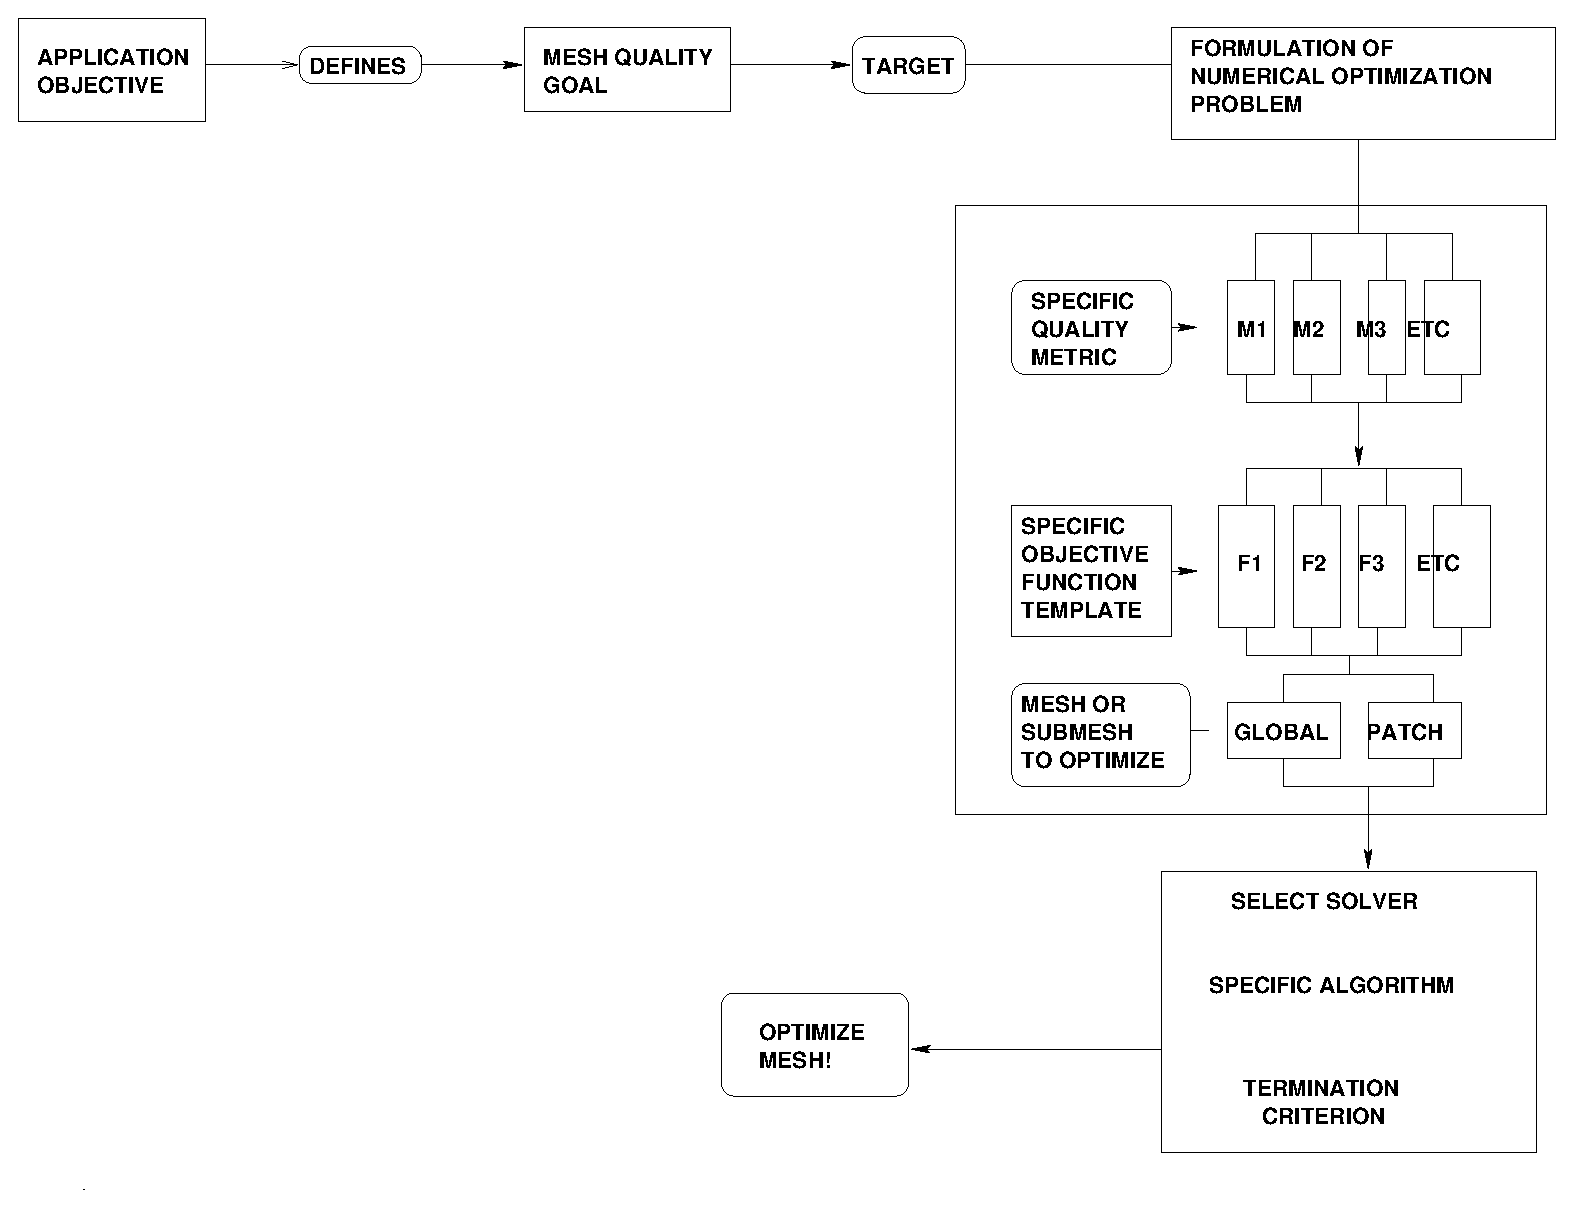
\includegraphics[width=4.7in]{figures/msq-paradigm}
\caption{\em The Mesquite Paradigm \label{Paradigm} }
%\end{tabular}
\end{center}
\end{figure}

\section{How to use this User's Manual}
This user's manual
\begin{itemize}
\item provides an introduction to mesh quality and basic Mesquite concepts (Chapter \ref{sec:intro}),
\item instructs novice users on how to download and install Mesquite (Chapter \ref{sec:install}),
\item provides a tutorial on Mesquite's simplified user's interface and Mesquite's detailed API (Chapter \ref{sec:examples}).
\item describes how to load a mesh in Mesquite via files (Chapter \ref{sec:meshes}), and
%\item provides instructions on using the extensive TSTT interface or a Mesquite mesh specific mesh
%      interface to load a mesh {\it dynamicallu} in Mesquite (sections \ref{sec:msq_mesh}, \ref{sec:TSTT}), and
\item describes Mesquite interactions with domain geometry (Chapter \ref{sec:geom}), and
\item describes Mesquite Wrappers (Chapter \ref{sec:wrappers}),
%\item Exposes in details the concepts and the mechanisms of the advanced API (chapter \ref{sec:API}), and
%\item instructs the user on how to add their own instances of quality
%metrics, objective functions, and solvers (chapter \ref{sec:extensions})
\end{itemize}

Consult the doxygen documentation for the API reference as well as details on the software. There
are two sets of doxygen documentations available:
\begin{itemize}
\item The developer doxygen doc is located in mesquite/doc/developer/. From that directory, you
      must run 'doxygen Mesquite.dox'.
\item The user doxygen doc (API doc) is located in mesquite/doc/user/doxygen. From that directory, you
      must run 'doxygen Mesquite-user.dox'.
\end{itemize}
The doxygen command will generate two directories: an html directory containing the file
index.html that you can open with your web browser, and a latex directory containing a Makefile that
will generate a dvi file.

%\section{Related Documents}

%Documentation of the Mesquite API can be generated from comments in the Mesquite
%source code using the Doxygen utility
%(\url{http://www.stack.nl/~dimitri/doxygen/}).
%To generate HTML and LaTeX copies of this documentation, execute the command
%{\tt doxygen Mesquite-user.dox} in the {\tt doc/usr/doxygen} subdirectory
%of the Mesquite source.

%Further information and related documentation are available on the
%Mesquite home page, located at:
%\url{http://www.cs.sandia.gov/optimization/knupp/Mesquite.html}.

\chapter{UNIFORM GENERATORS}

This chapter contains a description of various uniform generators
already programmed in this library and which were proposed by various 
authors over the past several years, as well as tools for managing
and implementing additional types of generators.
Related generators are regrouped in the same module.
For example, the linear congruential generators (LCGs) are in module
{\tt ulcg}, the multiple recursive generators (MRGs) are in {\tt umrg}, 
the inversive generators in {\tt uinv},
the cubic generators in {\tt ucubic}, etc.
We emphasize that the generators provided here are not all recommendable;
in fact, {\em most of them are not}.

The module {\tt unif01} contains the basic utilities for defining,
manipulating, filtering, combining, and timing generators.  
Each generator must be implemented as an 
object of type {\tt unif01\_Gen}.  To implement one's own generator,
one should create such an object and define all its fields.
For each generator, the structure {\tt unif01\_Gen} must contain a 
function {\tt GetU01} that returns values in the interval $[0,1)$
and a function {\tt GetBits} that returns a block of 32 bits.  
Most of the tests in the {\tt s} modules call the generators
to be tested only indirectly, through the use of the interface 
functions {\tt unif01\_StripD}, {\tt unif01\_StripL} and  
{\tt unif01\_StripB}.
These functions drop the $r$ most significant bits of each random number 
generated and returns a number built out of the remaining bits.

It is also possible to test one's own or an external generator
(that is, a generator that is not predefined in TestU01) very easily with
the help of the functions {\tt unif01\_CreateExternGen01} and
{\tt unif01\_CreateExternGenBits} (see page \pageref{externgen}
of this guide), as long as this generator is programmed in C.

Figure~\ref{fig:usegen} gives simple examples of how to use predefined
generators.  The program creates a LCG with modulus $m = 2^{31}-1$,
multiplier $a = 16807$, and initial state $s = 12345$,
generates and adds 100 uniforms produced by this generator,
prints the sum, and deletes the generator.
To illustrate the fact that there are different ways of getting the
uniforms from the generator, we have generated the first 50 by calling
the {\tt GetU01} function and the next 50 via {\tt unif01\_StripD}.
These two methods are equivalent.
The program then instantiates the generator {\tt lfsr113} available in 
module {\tt ulec}, with the vector $(12345, \ldots, 12345)$ as initial seed,
generates and prints five integers in the range $\{0,\dots,2^{10}-1\}$
(i.e., 10-bit integers) obtained by taking five successive output values
from the generator, stripping out the four most significant bits from 
each value, and retaining the next 10 bits.

For each public identifier used in programs, it is important to
include the corresponding header file before using it,
so as to inform the compiler about the type and signature of functions
and exported variables. For instance, in the following examples, the header
files \texttt{unif01.h}, \texttt{ulcg.h} and \texttt{ulec.h} contain the 
declarations of \texttt{unif01\_Gen}, \texttt{ulcg\_CreateLCG} and 
\texttt{ulec\_Createlfsr113}, respectively.
 
Other examples on how to use the facilities of module {\tt unif01} are given 
at the end of its description.


\setbox0=\vbox {\hsize = 6.0in
\smallc
\verbatiminput{../examples/ex1.c}
}

\begin{figure}
\centering
\myboxit{\box0}
\caption {Using pre-programmed generators\label {fig:usegen}}
\end{figure}


\iffalse  %%%%%%%
%%%%%%%%%%%%%%%%%%%%%%%%%%%%%%%%%%%%%%%%%%%%%%%%%%%%%%%%%%%%%%%

\section {La vitesse des generators}

Les Tableaux \ref{vitesse1}--\ref{vitesse10} donnent une idee 
du temps d'execution moyen
par appel (en micro-secondes), pour un certain number de generators
fournis par the modules {\tt u...}.
Ces values sont en fait le number de secondes
requises pour un million $(10^6)$ d'appels, 
donne ici a une seconde pres.
La machine utilisee etait un SUN UltraSparc 150.
%%  80386 avec coprocesseur 80387, tous deux a 16 MHz.
Pour fins de comparaison, pour un million d'appels a une procedure
``bidon'' ne faisant rien, dans le m\^eme contexte, il a fallu 0.26 secondes.

\begin{table}[htb] \centering \tt
\caption {\rm Vitesse moyenne par appel pour the generators 
          du module ulcg.}
\label {vitesse1}
\begin{tabular}{|l|r|c|l|r|}
\hline
&&&&\\
\multicolumn{1}{|c|}{\rm Generator} & $\mu$-sec. && {\rm Generator}
   & $\mu$-sec.\\
\hline \hline
&&&&\\
 LCG$^1$              &   1.03 && CombLEC2$^2$ &   4.55\\
 LCG$^2$              &   2.33 && CombLEC2$^3$ &  20.22\\
 LCG$^3$              &  10.91 && CombLEC3$^2$ &   6.60\\
 LCGFloat             &   0.80 &&              &  \\
 BigLCG               &  45.24 && CombWH2$^1$  &   2.49\\
 LCG2e31              &   0.98 && CombWH2$^2$  &   4.67\\            
 LCG2e32              &   0.95 && CombWH2$^3$  &  20.40\\            
 LCG2e31m1HD          &   1.73 && CombWH3$^2$  &   7.25\\          
 CombLEC2$^1$         &   2.22 &&              &       \\
&&&&\\
\hline
\end{tabular}

\begin {verse}
 $^1$ : $(m-1)a + c$ representable en {\tt LONGINT} (implantation directe).\\
 $^2$ : implantation utilisee lorsque $a (m\mod a) < m$.\\
 $^3$ : implantation utilisee dans the autres cas.\\
\end {verse}
\end {table}

\begin{table}[htb] \centering \tt
\caption {\rm Vitesse moyenne par appel pour the generators 
              du module umrg.}
\label {vitesse2}
\begin{tabular}{|l|r|c|l|r|}
\hline
&&&&\\
\multicolumn{1}{|c|}{\rm Generator} & $\mu$-sec. && {\rm Generator}
   & $\mu$-sec.\\
\hline \hline
&&&&\\
 MRG$^1$              &  12.36 && MRG$^3$      &   6.35\\
 MRG$^2$              &   4.13 && C2MRG        &  10.71\\
 LagFib               &   0.59 &&              &\\
\hline
\end{tabular}

\begin {verse}
 $^1$ : implantation generale.\\
 $^2$ : implantation plus rapide mentionnee dans {\tt SetMRG}.\\
 $^3$ : varie selon que $p - d < 32$ ou non et que $d < 32$ ou non.\\
\end {verse}
\end {table}


\begin{table}[htb] \centering \tt
\caption {\rm Vitesse moyenne par appel pour the generators du 
              module utaus.}
\label {vitesse3}
\begin{tabular}{|l|r|c|l|r|}
\hline
&&&&\\
\multicolumn{1}{|c|}{\rm Generator} & $\mu$-sec. && {\rm Generator}
   & $\mu$-sec.\\
\hline \hline
&&&&\\
 Taus                 &   0.69 && CombTaus3    &   1.60\\
 TausJ                &   3.52 && Tez95        &   1.48\\
 LongTaus             &   1.07 && TezLec91     &   1.17\\
 CombTaus2            &   1.17 && Tausme3a     &   1.49\\
&&&&\\
\hline
\end{tabular}

\end {table}

\begin{table}[htb] \centering \tt
\caption {\rm Vitesse moyenne par appel pour the generators 
              du module ugfsr.}
\label {vitesse4}
\begin{tabular}{|l|r|c|l|r|}
\hline
&&&&\\
\multicolumn{1}{|c|}{\rm Generator} & $\mu$-sec. && {\rm Generator}
   & $\mu$-sec.\\
\hline \hline
&&&&\\
 GFSR                 &   0.66 && Toot73       &   0.62\\
 TGFSR                &   0.81 && Fushimi90    &   0.67\\
 Ripley90             &   0.53 && Kirk81       &   0.65\\
&&&&\\
\hline
\end{tabular}

\end {table}

\begin{table}[htb] \centering \tt
\caption {\rm Vitesse moyenne par appel pour the generators 
              du module uinv.}
\label {vitesse5}
\begin{tabular}{|l|r|c|l|r|}
\hline
&&&&\\
\multicolumn{1}{|c|}{\rm Generator} & $\mu$-sec. && {\rm Generator}
   & $\mu$-sec.\\
\hline \hline
&&&&\\
 InvImpl              &  14.18 && InvExpl      &  14.77\\
 InvImpl2a            &  22.95 && InvExpl2a    &  35.21\\
 InvImpl2b            &  22.82 && InvExpl2b    &  27.46\\
 InvMRG               &  23.12 &&              &       \\
&&&&\\
\hline
\end{tabular}

\end {table}

\begin{table}[htb] \centering \tt
\caption {\rm Vitesse moyenne par appel pour the generators 
              du module uquad.}
\label {vitesse6}
\begin{tabular}{|l|r|c|l|r|}
\hline
&&&&\\
\multicolumn{1}{|c|}{\rm Generator} & $\mu$-sec. && {\rm Generator}
   & $\mu$-sec.\\
\hline \hline
&&&&\\
 Quadratic            &  13.81 && Quadratic2$^1$&  14.77\\
 Quadratic2           &   1.63 &&               &       \\
&&&&\\
\hline
\end{tabular}

\begin {verse}
$^1$ : implantation rapide : e = 32.\\
\end {verse}
\end {table}

\begin{table}[htb] \centering \tt
\caption {\rm Vitesse moyenne par appel pour the generators 
              du module ulec.}
\label {vitesse7}
\begin{tabular}{|l|r|c|l|r|}
\hline
&&&&\\
\multicolumn{1}{|c|}{\rm Generator} & $\mu$-sec. && {\rm Generator}
   & $\mu$-sec.\\
\hline \hline
&&&&\\
 CombLec88            &   2.98 && CombMRG96       &   5.47\\
 MRG93                &   3.31 && CombMRG96d      &  11.22\\
 CombLec88Float       &   1.38 && CombMRG96Float  &   2.60\\
                      &        && CombMRG96dFloat &   5.13\\
&&&&\\
\hline
\end{tabular}

\end {table}

\begin{table}[htb] \centering \tt
\caption {\rm Vitesse moyenne par appel pour the generators 
              du module ucarry.}
\label {vitesse8a}
\begin{tabular}{|l|r|c|l|r|}
\hline
&&&&\\
\multicolumn{1}{|c|}{\rm Generator} & $\mu$-sec. && {\rm Generator}
   & $\mu$-sec.\\
\hline \hline
&&&&\\
 AWC                  &   0.85 && MWC$^1$      &  13.03\\
 SWC                  &   0.85 && SWC$^1$      &   3.79\\
&&&&\\
\hline
\end{tabular}

\begin {verse} 
 $^1$ : implantation generale, e = 32.\\
\end {verse} 
\end {table}

\begin{table}[htb] \centering \tt
\caption {\rm Vitesse moyenne par appel pour the generators 
              du module umarsa.}
\label {vitesse8}
\begin{tabular}{|l|r|c|l|r|}
\hline
&&&&\\
\multicolumn{1}{|c|}{\rm Generator} & $\mu$-sec. && {\rm Generator}
   & $\mu$-sec.\\
\hline \hline
&&&&\\
 KISS                 &   0.76 && Combo        &   1.15\\
 Marsa90a             &   0.87 && ECG1         &   1.34\\
 Marsa90b             &   0.83 && ECG2         &   1.31\\
 Mother0              &   1.77 && ECG3         &   1.39\\
                       &&& ECG4                &   1.36 \\
% Mother1$^1$          &   5.95 &&              &       \\
&&&&\\
\hline
\end{tabular}
\end {table}

\begin{table}[htb] \centering \tt
\caption {\rm Vitesse moyenne par appel pour the generators 
              du module unumrec.}
\label {vitesse9}
\begin{tabular}{|l|r|c|l|r|}
\hline
&&&&\\
\multicolumn{1}{|c|}{\rm Generator} & $\mu$-sec. && {\rm Generator}
   & $\mu$-sec.\\
\hline \hline
&&&&\\
 Setran0              &   2.33 &&  Setran2      &   5.25\\
 Setran1              &   2.91 &&               &       \\
&&&&\\
\hline
\end{tabular}

\end {table}

\begin{table}[htb] \centering \tt
\caption {\rm Vitesse moyenne par appel pour the generators 
              des modules uvaria et ufile.}
\label {vitesse10}
\begin{tabular}{|l|r|c|l|r|}
\hline
&&&&\\
\multicolumn{1}{|c|}{\rm Generator} & $\mu$-sec. && {\rm Generator}
   & $\mu$-sec.\\
\hline \hline
&&&&\\
 Tindo                &  64.31 && ACORN        &  75.33\\
 CSD                  &   6.03 && ReadFile     &  13.82\\
&&&&\\
\hline
\end{tabular}

\end {table}

\fi   %%%%%%%%%%%%%%%%%%%%

\defmodule {unif01}

This module offers basic tools for defining, manipulating, and
transforming uniform random number generators to which tests are 
to be applied or which could be used for other purposes.
Each generator is implemented as a
structure of type {\tt unif01\_Gen}. 
Several predefined generators are available in the {\tt u} modules.
Each such generator must be created by the appropriate 
{\tt \ldots Create\ldots} function before being used, and should
be deleted by the corresponding {\tt \ldots Delete\ldots} function
to free the memory used by the generator when it is no longer needed.
One can create and use simultaneously any number of generators. 
These generators are usually passed to functions as pointers to
objects of type {\tt unif01\_Gen}.

One may call an external generator for testing using the functions in
this module. See Figure~\ref{prog:ex7} for an example.
One may also implement one's own generator, by creating a structure of 
type {\tt unif01\_Gen} and defining all its fields properly.
See Figure~\ref{fig:my16807} for an illustration.

Each implemented generator returns either a floating-point 
number in $[0, 1)$ (via its function {\tt GetU01}) 
or a block of 32 bits (via its function {\tt GetBits}).
Ideally, these should follow the uniform distribution $(0,1)$
and $\{0,\dots,2^{32}-1\}$, respectively.
Most of the tests in the {\tt s} modules actually call the generator
to be tested only indirectly through the use of one of the interface 
functions {\tt unif01\_StripD},
 {\tt unif01\_StripL} and  {\tt unif01\_StripB}.
These functions drop the $r$ most significant bits of each random number 
and return a number built out of the remaining bits.

Functions are also provided for adding one or many output {\em filters\/} 
to a given generator. These functions create another generator
object which implements a mechanism that automatically
transforms the output values of the original generator in a specified way.
One can also combine the outputs of several generators in different ways.
By using the output of several generators or several substreams of the
same generator in a round-robin way, one can test the quality of these as 
examples of parallel generators.
Finally, tools are provided for measuring the speed of generators
and adding their output values (for testing purposes).



%%%%%%%%%%%%%
\bigskip\hrule
\code\hide
/*  unif01.h  for ANSI C  */
#ifndef UNIF01_H
#define UNIF01_H
\endhide
#include "gdef.h"
\endcode


%%%%%%%%%%%%%%%%%%%%%%%%%%%%%%%%%%%%%%%%%%
\guisec{Basic types}
\code

typedef struct {
   void *state;
   void *param;
   char *name;
   double (*GetU01) (void *param, void *state);
   unsigned long (*GetBits) (void *param, void *state);
   void (*Write) (void *state);
} unif01_Gen;
\endcode
  \tab Generic random number generator. The function {\tt GetU01}
   returns a floating-point number in $[0,1)$ while {\tt GetBits}
   returns a block of 32 bits. If the generator delivers less than 32
   bits, these bits are left shifted so that the most
   significant bits are the relevant ones.
% If the generator returns less than 32 bits of precision, then one must make
% sure that these bits are the most significant bits of the returned block.
   The variable {\tt state} keeps the
   current state of the generator and {\tt param} is the set of
   specific parameters used in computing the next random number. 
   The function  {\tt Write} will write the current state of the
   generator. The string  {\tt name}  describes the current generator,
   its parameters, and its initial state.
   In the description of the generators in the u modules, one
   indicates how the {\tt GetU01} function  gets its value from the
   generator's recurrence;
   it is always understood that the {\tt GetBits}  function is
   equivalent to $2^{32}\,${\tt GetU01}.
  \endtab

%%%%%%%%%%%%%%%%%%%%%%%%%%%%%%%%%%%%%%%%%%
\guisec{Environment variables}

\ifdetailed
\code

#define unif01_MASK32  0xffffffffUL
\endcode
  \tab 32-bit mask.
 \endtab
\code


#define unif01_NORM32  4294967296.0
#define unif01_INV32   2.328306436538696289e-10
\endcode 
 \tab The constants $2^{32}$ and $1/2^{32}$ respectively: 
   normalization factors used in many generators to transform
  a floating-point ``random'' number into a 32-bit integer, or vice-versa.
 \endtab
\fi

\code


extern lebool unif01_WrLongStateFlag;
\endcode
  \tab For generators whose state is a large array, determines whether
   the state will be written out in full ({\tt TRUE}) or not ({\tt FALSE})
   in the printouts. The default value is {\tt FALSE}. 
\hrichard{C'est la seule variable globale qui reste. On pourrait
  l'\'eliminer en ajoutant un argument \`a unif01\_Gen.Write, qui
  deviendrait  {\tt Write (void *state, lebool flag).}}
 \endtab



%%%%%%%%%%%%%%%%%%%%%%%%%%%%%%%%%%%%%%%%%%
\guisec{Basic functions}

\code


double unif01_StripD (unif01_Gen *gen, int r);
\endcode
\tab Makes one call to the generator {\tt gen}, drops the $r$ most
  significant bits, left-shift the others by $r$ positions, and
  returns the result, which is a floating-point number in $[0,1)$.
 More specifically, returns $2^r u \mod 1$, 
 where $u$ is the output of {\tt gen}.
 \endtab
\code


long unif01_StripL (unif01_Gen *gen, int r, long d);
\endcode
\tab
 Similar to {\tt unif01\_StripD}, but generates an integer ``uniformly'' over
 the set $\{0,\dots,d-1\}$, by using the most significant bits of the
 output of {\tt gen} after having dropped the first $r$ bits.
 More specifically, returns $\lfloor d (2^r u \mod 1)\rfloor$, 
 where $u$ is the output of {\tt gen}.
\endtab
\code


unsigned long unif01_StripB (unif01_Gen *gen, int r, int s);
\endcode
\tab
 Calls the generator {\tt gen}, drops the $r$ most significant bits,
 and returns the $s$ following bits as an integer in 
 the set $\{0,\dots,2^s-1\}$.
\endtab
\code


void unif01_WriteNameGen (unif01_Gen *gen);
\endcode
 \tab  Writes the character string {\tt gen->name} that describes the
  generator.
 \endtab
\code


void unif01_WriteState (unif01_Gen *gen);
\endcode
 \tab  Writes the current state of generator  {\tt gen}.
 \endtab
\code


void unif01_WrLongStateDef (void);
\endcode
 \tab Dummy function used when the state of the current
   generator is a large array and we do not want to write the full state.
   Writes the message ``{\tt   Not shown here ... takes too much space}''.
 \endtab
\code


unif01_Gen * unif01_CreateDummyGen (void);
\endcode
\tab  Creates a {\em dummy\/} generator, which does nothing and always
\index{Generator!dummy}%
  returns zero. It can be used for instance to measure the overhead of
  function calls when comparing generator's speeds
  (see the timing tools below).
\endtab
\code


void unif01_DeleteDummyGen (unif01_Gen *gen);
\endcode
\tab  Frees the dynamic memory used by the dummy generator above.
\endtab
\ifdetailed
\code


void unif01_DeleteGen (unif01_Gen *gen); 
\endcode 
\tab  Frees the dynamic memory used by a typical generator, for which
  the state does not contain dynamically allocated arrays. 
  In this case, the memory
  is allocated by a {\tt u\ldots\_Create\ldots} function in some
  {\tt u} module and the present function is called by the corresponding
  {\tt u\ldots\_Delete\ldots} function in the same {\tt u} module.
\endtab
\fi



%%%%%%%%%%%%%%%%%%%%%%%%%%%%%%%%%%%%%%%%%%
\guisec{Output filters}

The following describes some filters that can be added to transform 
the output of a given generator. In each case, a new generator object is
created that will effectively apply the filter to the original generator.
One may apply more than one filter at a time on a given generator
(for example, one may apply the {\tt Double}, the  {\tt Bias}, the 
 {\tt Trunc} and the {\tt Lac} filters on top of one another). It suffices
 to create the appropriate filters as described below.  The resulting 
filtered generator(s) will call the original generator behind the scenes.
Thus the state of the original generator will evolve as usual, even
though it is not called directly.\index{filters}


The different filters applied on an original generator are not independent
but are related as the elements of a stack. When they are no longer in use, 
they must be deleted {\em in the reverse order of their creation}, 
the original generator being the last one of this group to be deleted. 
Figure~\ref{fig:prog-filter} illustrates how these facilities can be used.

\code


unif01_Gen * unif01_CreateDoubleGen (unif01_Gen *gen, int s);
\endcode
 \tab
 Given a generator {\tt gen}, this function
\index{Generator!filter!increased precision}%
 creates and returns a generator with increased precision, such that
 every call to this new generator
 corresponds to two successive calls  to the original generator.
 The method {\tt GetU01} of this doubled generator  returns
 $(U_1 +  U_2/2^s)$ mod 1, where $U_1$ and $U_2$ are the results of
 two successive calls  to the method {\tt GetU01} of {\tt gen}. 
 If the current generator has 31 bits of precision, for example,
 then one can obtain 53 bits of precision from {\tt GetU01} 
 by creating this new generator with {\tt s}  between $22$ and $31$.
% Not true anymore:
%  The function {\tt GetBits} of this new generator 
%  will return  $(X_1 +  X_2/2^s)$ mod $2^{32}$,
%  where $X_1$ and $X_2$ are the results of two successive calls to  the
%  method  {\tt GetBits} of the original {\tt gen}.
%  So it may return  more bits of precision, but never more than 32 bits.  
 \endtab
\code


unif01_Gen * unif01_CreateDoubleGen2 (unif01_Gen *gen, double h);
\endcode
 \tab A more general version of {\tt unif01\_CreateDoubleGen} where
  the method {\tt GetU01} of the double generator  returns
  $(U_1 +  h U_2)$ mod 1. Restriction: $0 < h < 1$.
 \endtab
\code


unif01_Gen * unif01_CreateLacGen (unif01_Gen *gen, int k, long I[]);
\endcode
 \tab
  Given an original generator {\tt gen}, this function 
\index{Generator!filter!lacunary indices}%
  creates and returns a generator involving lacunary indices, such that
  successive calls to this new generator
  will no longer provide successive values from the original
  generator, but rather selected values as specified by
  the table {\tt I[0..k-1]}, in a circular fashion.
  More specifically, if $u_0, u_1, u_2, \dots$ is the sequence
  produced by the original {\tt gen}, if the table {\tt I[0..k-1]}
  contains the non-negative integers $i_0, \dots i_{k-1}$ (in increasing
  order), and if we put $L = i_{k-1}+1$,
  then the output sequence of the new generator will be:
   $$ u_{i_0}, u_{i_1}, \dots, u_{i_{k-1}}, u_{L+i_0}, u_{L+i_1},
      \dots, u_{L+i_{k-1}}, u_{2L+i_0}, u_{2L+i_1}, \dots. $$
  For example, if  $k=3$ and $I = \{0, 3, 5\}$,
  the output sequence will be the numbers
   $$ u_{0}, u_{3}, u_{5}, u_{6}, u_{9}, u_{11}, u_{12}, \dots $$
  of the original generator.
  To obtain every $s$-th number produced by the original generator
  for example (a {\em decimated sequence\/}), one should take
  $k=1$ and $I = \{s-1\}$.
%  (note that taking $I = \{0, s\}$ won't work; it would return
%  $u_0, u_s, u_{s+1}, u_{2s+1}, \dots$).
 \endtab
\code


unif01_Gen * unif01_CreateLuxGen (unif01_Gen *gen, int k, int L);
\endcode
 \tab   Given an original generator {\tt gen}, this function
\index{Generator!filter!luxury}% 
  creates and returns a new generator giving the output of the
  original generator with luxury level $L$: out of every group of $L$
  random numbers, the first $k$ are kept and the next $L-k$ are skipped.
 \endtab
\code


unif01_Gen * unif01_CreateBiasGen (unif01_Gen *gen, double a, double p);
\endcode
 \tab  Given an original generator {\tt gen}, this function 
  creates and returns a new generator giving a biased output of the
  original generator.  The output is biased 
\index{Generator!filter!biased output}%
  in such a way that the density becomes
  constant with total probability $p$ over the interval $[0, a)$, and
  constant with total probability $1 - p$ over $[a, 1)$ (the two constant
  densities are different). For example, by choosing $p= 1$ and $a = 0.5$,
  all the random numbers generated by {\tt GetU01} will fall
  on the interval $[0,\; 0.5)$. This filter can be used, for example,
  to study the power of certain statistical tests.
  Restrictions: $0 < a < 1$ and $0 \le p \le 1$.
 \endtab
\code


unif01_Gen * unif01_CreateTruncGen (unif01_Gen *gen, int s);
\endcode
 \tab   Given an original generator {\tt gen}, this function
\index{Generator!filter!bit truncated}% 
  creates and returns a new generator giving the output of the
  original generator truncated to its $s$ most significant bits.
 Restriction: $s \le 32$.
\endtab
\code


unif01_Gen * unif01_CreateBitBlockGen (unif01_Gen *gen, int r, int s,
                                       int w);
\endcode
 \tab  Consider a group of $v \le 32$ successive 32-bit integers
  outputted by generator {\tt gen}. For each of these, drop the $r$ most
\index{Generator!filter!blocks of bits}% 
  significant bits and keep the $s$ following bits numbered
  $b_{i 1}, b_{i 2}, \ldots, b_{i s}$, starting with the
  most significant, for $1 \le i \le v$.
  Make with all these a $v\times s$ matrix of bits, say ${\cal B}$.
  The generator returned by this function is a filter that builds new 32-bit
   integers from $v\times w$ submatrices of ${\cal B}$. 
  The number of columns of the submatrix $w$ must be a power of 2 no larger
  than 32 and it must be $\le s$. If $w$ does not divide $s$ exactly,
  the last submatrix of ${\cal B}$ will have less than $w$ columns and
  will be disregarded.

  If the stream of bits thus obtained from {\tt gen} is
  $$
   b_{1 1}, b_{1 2}, \ldots,  b_{1 s},
   b_{2 1}, b_{2 2}, \ldots,  b_{2 s},
   \ldots,
   b_{v 1}, b_{v 2}, \ldots,  b_{v s}, \ldots
$$
   then the new integers returned by the filter will be 32-bit integers
   taken from the rearranged stream of bits so that the first new 
   number is (its most significant bit being given first)
  $$
   b_{1 1}, b_{1 2}, \ldots,  b_{1 w},
   b_{2 1}, b_{2 2}, \ldots,  b_{2 w},
   \ldots,
   b_{v 1}, b_{v 2}, \ldots,  b_{v w},
$$
  the second new  number is made of the bits (its most
  significant bit first)
  $$
   b_{1 (w+1)}, b_{1 (w+2)}, \ldots,  b_{1 (2w)},
   b_{2 (w+1)}, b_{2 (w+2)}, \ldots,  b_{2 (2w)},
   \ldots,
   b_{v (w+1)}, b_{v (w+2)}, \ldots,  b_{v (2w)},
  $$
  and so on.

  The following examples illustrates how the filter works.
  If $r$ = 0 and $w = s = 32$, then the filter has no effect,
  the new integers being the same as those outputted by  {\tt gen}.
  If $r$ = 0 and $w = s = 1$, then the filter will return integers
  made only from the most significant bit of the original integers, all 
  other bits being dropped.
  If $r$ = 0, $w = 1$ and $ s = 32$, then the filter will return integers
  made from the columns of ${\cal B}$, i.e., since the rows of ${\cal B}$
  are made of the original integers, the filter will return the columns
  of ${\cal B}$ as the new integers. 
  Restrictions: $r \ge 0$, $0 < s \le 32$ and
   $w$ in  $\{1, 2, 4, 8, 16, 32\}$.
 \endtab
\code


void unif01_DeleteDoubleGen (unif01_Gen *gen);
void unif01_DeleteLacGen    (unif01_Gen *gen);
void unif01_DeleteLuxGen    (unif01_Gen *gen);
void unif01_DeleteBiasGen   (unif01_Gen *gen);
void unif01_DeleteTruncGen  (unif01_Gen *gen);
void unif01_DeleteBitBlockGen (unif01_Gen *gen);
\endcode
 \tab Frees the memory used by the generator created by the corresponding
 {\tt Create} functions above.
 \endtab



%%%%%%%%%%%%%%%%%%%%%%%%%%
\guisec{Combining generators}

These functions permit one to define the combination of two, three 
or more generators. The resulting generator calls
\index{Generator!combined}\index{combined generators}% 
the component generators behind the scenes, so it changes their
state. \emph{The  component generators must not be destroyed as long as the
 combination generator is in use.}
One can obtain the combinations of more than three generators by combining
the generators obtained from combinations of two or three generators.
%
\hide
\code

typedef struct {
   unif01_Gen *gen1;
   unif01_Gen *gen2;
} unif01_Comb2_Param;
\endcode 
 \tab This is used for combining two arbitrary generators. It is made
  public because it would not be possible otherwise to free the dynamic
  memory used by the two component generators when they are programmed
  in another module.
  \endtab
\endhide
\code


unif01_Gen * unif01_CreateCombAdd2 (unif01_Gen *gen1, unif01_Gen *gen2,
                                    char *name);
\endcode
 \tab  This function creates and returns a generator whose output is the
 addition of the outputs modulo 1 of the  method {\tt GetU01} of the 
 two generators {\tt gen1} and {\tt gen2}.
 The character string {\tt name} may be printed in reports to identify this
 new combined  generator.
\index{combined generators!addition}
 \endtab
\code


unif01_Gen * unif01_CreateCombAdd3 (unif01_Gen *gen1, unif01_Gen *gen2,
                                    unif01_Gen *gen3, char *name);
\endcode
 \tab  Same as {\tt unif01\_CreateCombAdd2}, except that the returned
  generator is the combination (the addition of the outputs modulo 1 of the
  method {\tt GetU01}) of the three generators {\tt gen1, gen2} and {\tt gen3}.
\hrichard{
  When the combined generator is used to generate random integers, in rare
  cases, an integer may differ by 1 unit depending on the order of
   addition of the 3 terms (one from each component). This is due
   to the last bit (bit 53) of the value returned which may be affected by
   floating-point numerical errors. Furthermore, the result
   may be different if the addition is done without function calls
   (as in the pre-programmed version of Wichmann-Hill for example in
   {\tt ulcg\_CreateCombWH3}), in  which
   case, the 2 extra guard bits required by the IEEE-754 standard in
   floating-point arithmetic operations may give a more exact result.
}
 \endtab
\code


unif01_Gen * unif01_CreateCombXor2 (unif01_Gen *gen1, unif01_Gen *gen2,
                                    char *name);
\endcode
 \tab  This function creates and returns a generator whose output is the
 bitwise {\sl exclusive-or (XOR)\/}  of the outputs of the two generators
 {\tt gen1} and {\tt gen2}. The character string {\tt name} may be printed
 in reports to identify this combined generator.
 \index{combined generators!exclusive or}
 \endtab
\code


unif01_Gen * unif01_CreateCombXor3 (unif01_Gen *gen1, unif01_Gen *gen2,
                                    unif01_Gen *gen3, char *name);
\endcode
 \tab  Same as {\tt unif01\_CreateCombXor2}, except that the 
 returned generator is the combination of the three generators
 {\tt gen1, gen2} and {\tt gen3}.
 \endtab
\code


void unif01_DeleteCombGen (unif01_Gen *gen);
\endcode
 \tab  Frees the memory used by one of the combination generators returned
  by the  {\tt Create} functions above, but does not delete any of its
  component generators.
 \endtab


%%%%%%%%%%%%%%%%%%%%%%%%%%
\guisec{Parallel generators}

 The following functions allow the joining of the output of several generators
 or of different substreams of the same generator into a single stream of
 random numbers. This can be used to test for apparent correlations between the
 output of several generators or several substreams used in parallel.
 For example, one may want to choose seeds 
 that are far separated for the same generator, while making sure that 
 such seed choice is statistically valid and does not introduce unwanted 
 correlation between the substreams thus defined.
\code

unif01_Gen * unif01_CreateParallelGen (int k, unif01_Gen *gen[], int L);
\endcode
 \tab Creates and returns a generator whose output is obtained in a round-robin
  way $L$ numbers at a time from each of the $k$ generators \texttt{gen[i]} as 
  follows: the first $L$ numbers are generated from \texttt{gen[0]}, the next 
  $L$ numbers are generated from \texttt{gen[1]}, and so on until 
  $L$ numbers have been generated from \texttt{gen[k-1]}, after which, this whole
  process is repeated. \emph{It is important that none of the generators} 
 \texttt{gen[i]} \emph{be destroyed as long as the parallel generator is in use.}
 \endtab
\code


void unif01_DeleteParallelGen (unif01_Gen *gen);
\endcode
 \tab  Frees the memory allocated by the parallel generator returned
  by the  {\tt Create} function above, but \emph{does not} delete any of its
  component generators, which is the responsibility of the program that
  created them.
 \endtab


%%%%%%%%%%%%%%%%%%%%%%%%%%
\guisec{External generators}

Although  TestU01 implements many generators both in generic and in
specific forms, it is not possible to implement all those that are in
existence because there are just too many and new ones are proposed 
regularly. The typical user would like to test his preferred generator
with as little complications as possible. The functions below allows one 
to do just that. As long as the generator is programmed in C, 
one has but to pass  the function implementing the generator to one of the
functions below and call some of the tests available in TestU01.
It is the responsibility of the user to ensure that his generator does not
violate the conditions described in the functions below. For the
call in {\tt unif01\_CreateExternGen01}, his generator must return
floating-point numbers in $[0, 1)$. For the calls in
 {\tt unif01\_CreateExternGenBitsL} and  {\tt unif01\_CreateExternGenBits},
 his generator must return an integer in the interval $[0, 2^{32} - 1]$.
If these conditions are violated, the results of the tests in TestU01 are
unpredictable. % Similarly, a generator should not be so pathological so as to
% return the same value at every call. 
 \index{Generator!user defined} \index{Generator!external}%
\code


unif01_Gen *unif01_CreateExternGen01 (char *name, double (*gen01)(void*,void*),
                                      unsigned long (*gen01_bits)(void*,void*));
\endcode
\tab Implements a pre-existing external generator {\tt gen01} that is
  not part of TestU01. \label{externgen}
 It must be a C function taking no argument and returning a {\tt double}
 in the interval $[0, 1)$. Parameter {\tt name} is the name of the generator.
 No more than one generator of this type can be in use at a  time. 
\endtab
\code


unif01_Gen *unif01_CreateExternGenBits (char *name,
                                        unsigned int (*genB)(void));
\endcode
\tab Implements a pre-existing external generator {\tt genB} that is not part
 of TestU01. It must be a C function taking no argument and returning
 an integer in the interval $[0, 2^{32} - 1]$.
 If the generator delivers less than 32 bits of resolution, then these 
 bits must be left shifted so that the most significant bit is bit 31
 (counting from 0). Parameter {\tt name} is the name of the generator.
 No more than one generator of this type can be in use at a  time. 
 \endtab
\code


unif01_Gen *unif01_CreateExternGenBitsL (char *name,
                                         unsigned long (*genB)(void));
\endcode
\tab Similar to {\tt unif01\_CreateExternGenBits}, but with
{\tt unsigned long} instead of {\tt unsigned int}. The generator 
{\tt genB} must also return  an integer in the interval $[0, 2^{32} - 1]$.
 \endtab
\code


void unif01_DeleteExternGen01 (unif01_Gen * gen);
void unif01_DeleteExternGenBits (unif01_Gen * gen);
void unif01_DeleteExternGenBitsL (unif01_Gen * gen);
\endcode
 \tab  Frees the memory used by the generator created by the corresponding
 {\tt Create} functions above.
 \endtab


\bigskip
As an example, Figure~\ref{prog:ex7}  shows how to apply
 {\tt SmallCrush}, a small predefined battery of tests (described on page
 \pageref{bat:SmallCrush}) to the generators {\tt MRG32k3a} and {\tt
xorshift}, whose code is shown in Figures~\ref{fig:MRG32k3a} and
 \ref{fig:xorshift}.  One must compile and link the two external
files with the main program and the TestU01 library.
The generator {\tt MRG32k3a} returns numbers in (0, 1) and was
proposed by L'Ecuyer in \cite{rLEC99b}.
The generator {\tt xorshift} returns 32-bit integers 
and was proposed by Marsaglia in \cite[page 4]{rMAR03a}.


%%%%%%%%%%%%%%%%%%%%%%%%%%%%%%%%%%%%%%%%%%%%%%

\setbox0=\vbox {\hsize = 6.2in
{\smallc
\verbatiminput{../examples/ex7.c}}
}

\begin{figure} \centering \myboxit{\box0}
\caption {Example of a program to test two external generators}
\label {prog:ex7}
\end{figure}


\setbox1=\vbox {\hsize = 6.2in
{\smallc
\verbatiminput{../examples/mrg32k3a.c}}
}

\begin{figure} \centering \myboxit{\box1}
\caption {External function for {\tt MRG32k3a}.}
\label {fig:MRG32k3a}
\end{figure}


\setbox1=\vbox {\hsize = 6.2in
{\smallc
\verbatiminput{../examples/xorshift.c}}
}

\begin{figure} \centering \myboxit{\box1}
\caption {External function for {\tt xorshift}.}
\label {fig:xorshift}
\end{figure}


%%%%%%%%%%%%%%%%%%%%%%%%%%%%%%%%%%%%%%%%%%%%%%
\guisec{Timing devices}

\code

typedef struct {
   unif01_Gen *gen;
   long n;
   double time;
   double mean;
   lebool fU01;
   } unif01_TimerRec;
\endcode
 \tab  Structure to memorize the results of speed and sum tests on a given
   generator. Here, {\tt gen} is the generator,\index{timer}
   {\tt n} is the number of calls made to the generator,
   {\tt time} is the total CPU time in seconds, and
   {\tt mean} is the mean of the {\tt n} output values of the generator.
   If {\tt fU01} is  {\tt TRUE}, the function {\tt GetU01} of 
   {\tt gen} is called, otherwise the function  {\tt GetBits} is called.
 \endtab
\code


void unif01_TimerGen (unif01_Gen *gen, unif01_TimerRec *timer, long n,
                      lebool fU01);
\endcode
 \tab
 This function computes the CPU time needed to generate
\index{Generator!speed}\index{Generator!timing}%
  {\tt n} random numbers with the generator {\tt gen},
  and returns the result in {\tt timer}. If {\tt fU01} is  {\tt TRUE},
  the random numbers will be generated by the method {\tt GetU01} of 
  {\tt gen}, otherwise by the
  method  {\tt GetBits}.
 \endtab
\code


void unif01_TimerSumGen (unif01_Gen *gen, unif01_TimerRec *timer, long n,
                         lebool fU01);
\endcode
 \tab
  Same as {\tt unif01\_TimerGen}, but also adds the {\tt n} random
  numbers and saves their mean in {\tt timer->mean}.
 \endtab
\code


void unif01_WriteTimerRec (unif01_TimerRec *timer);
\endcode
 \tab
  Prints the results contained in {\tt timer}, with some information
  about the generator and the current machine. One should make sure that the
  generator {\tt gen} in {\tt timer} has not been deleted when
  calling this function. 
\hrichard {Ceci m'inqui\`ete un peu, car si
l'utilisateur appelle cette fonction apr\`es que le g\'en\'erateur 
ait \'et\'e d\'etruit, il y aura un {\tt segmentation fault}. L'alternative
serait de r\'eserver un tableau de 50 caract\`eres dans 
{\tt unif01\_TimerRec} et d'y recopier le nom du g\'en\'erateur, au lieu
d'avoir le pointeur {\tt gen}.}
 \endtab
\code


void unif01_TimerGenWr (unif01_Gen *gen, long n, lebool fU01);
\endcode
 \tab
  Equivalent to calling {\tt unif\_TimerGen} followed by 
  {\tt unif01\_WriteTimerRec}. 
 \endtab
\code


void unif01_TimerSumGenWr (unif01_Gen *gen, long n, lebool fU01);
\endcode
 \tab
  Equivalent to calling {\tt unif\_TimerSumGen} followed by 
  {\tt unif01\_WriteTimerRec}. 
 \endtab
\code
\hide
#endif
\endhide
\endcode

%%%%%%%%%%%%%%%%%%%%%%%%%%%%%%%%%%%%%%%%%%%%%%%%%%%%%%%%%%%%%

\subsection*{Examples}

We now provide some examples of how to use the facilities of {\tt unif01}.
Figure~\ref{fig:my16807} gives an example of how to implement one's own
generator, using all the paraphernalia of TestU01. This is specially
useful when one wants to implement a generator in generic form with
one or more parameters.
 This is a simple LCG with hardcoded parameters $m=2^{31}-1$ 
and $a = 16807$.\index{Generator!user defined}
The function {\tt My16807\_U01} will advance the generator's state
by one step and return a $U(0,1)$ random number $U$ each time it is
called, whereas {\tt My16807\_Bits} will return the 32 most significant
bits in the binary representation of $U$.
The function {\tt CreateMy16807} allocates the memory for the corresponding
{\tt unif01\_Gen} structure and initializes all its fields.


\setbox2=\vbox {\hsize = 6.2in
{\smallc
\verbatiminput{../examples/my16807.c}}
}

\begin{figure} \centering \myboxit{\box2}
\caption {A user-defined generator, in file {\tt my16807.c}.}
\label {fig:my16807}
\end{figure}


%%%%%%%%%%%%%%%%%%%%%%%%%%%%%%%%%%%%%%%%%%%%%

Figure~\ref{fig:unif-timing} shows how to use the timing facilities.
The {\tt main} program first sets the generator {\tt gen} to an LCG
with modulus $2^{31}-1$, multiplier $a = 16807$, and initial state 12345,
implemented in floating point. 
\hrichard {Sur ma machine Linux, le
   LCG (en entiers) est 12\% plus rapide que la version LCGFloat} 
(This generator is well known, but certainly {\em not\/} to be recommended;
its period length of $2^{31}-2$ is much too small.)
The program calls {\tt unif01\_TimerSumGenWr} which generates 10 million 
random numbers in $[0, 1)$, computes their mean, and prints the CPU time 
needed to do that.
Next, the program deletes this {\tt unif01\_Gen} object and creates a 
new one, which is actually a user-defined implementation of the same LCG,
taken from the home-made module {\tt my16807} whose code is shown in
Figure~\ref{fig:my16807}.
In this implementation, the parameters have been placed as constants 
directly into the code.
Ten million random numbers are generated with this alternative 
implementation, and the average and CPU time are printed.
The same procedure is repeated for two additional predefined
generators taken from modules {\tt ulec}.
% with period lengths near $2^{191}$ and near $2^{113}$, respectively. 
Figure~\ref{fig:unif-timing-res} shows the results of this program,
run on a 2106 MHz computer running Linux, and compiled with {\tt gcc -O2}.


%%%%%%%%%%%%%%%%%%%%%%%%%%%%%%%%%%%%%%%%%%%%%%

\setbox0=\vbox {\hsize = 6.2in
{\smallc
\verbatiminput{../examples/ex3.c}}
}

\begin{figure} \centering \myboxit{\box0}
\caption {Example of a program creating and timing generators.}
\label {fig:unif-timing}
\end{figure}


\setbox1=\vbox {\hsize = 6.2in
{\smallc
\verbatiminput{../examples/ex3.res}}
}

\begin{figure} \centering \myboxit{\box1}
\caption {Results of the program of Figure~\ref{fig:unif-timing}.}
\label {fig:unif-timing-res}
\end{figure}


%%%%%%%%%%%%%%%%%%%%%%%%%%%%%%%%%%%%%%%%%%%%%

Figure~\ref{fig:prog-filter} shows how to apply filters to generators
and how to combine two or more generators by addition modulo 1 or bitwise
exclusive-or.
The program starts by creating a simple Tausworthe generator {\tt gen1}
and it generates 20 values from it.
It then deletes {\tt gen1}, creates a new copy of it with the same 
parameters and initial state, and applies a ``lacunary indices'' 
filter to create a second generator {\tt gen2}.  
The output sequence of {\tt gen2} will be 
(in terms of the original sequence numbering)
$u_3, u_7, u_9, u_{13}, u_{17}, u_{19}, u_{23}, \dots$.
Next, the program creates a generator {\tt gen3} for which each output value
is constructed from two successive output values of {\tt gen2},
generates some values from {\tt gen3} and {\tt gen2}, and deletes them.
%
\hpierre{I would like to generate and print 20 numbers from {\tt gen1}, 
    then reset {\tt gen1} to its initial state, then 
    generate and print 20 numbers from {\tt gen2}.
    But there is no public facility to reset a generator to a given state!
    To implement such facilities, we would have to make public the
    structure type that represents the state, for each type of generator.
    Presently, these types are hidden in the .c}
\hrichard{Peut-\^etre qu'il ne serait pas n\'ecessaire de rendre le type
 de l'\'etat public. Il faudrait toutefois une fonction {\tt Init} dans 
 la structure  {\tt unif01\_Gen}.}

After that, the program creates another Tausworthe generator {\tt gen2}
and a generator {\tt gen3} which is a combination of {\tt gen1} and 
{\tt gen2} by bitwise exclusive-or.  It generates a few values with
{\tt gen3} and deletes all the generators.



\setbox10=\vbox {\hsize = 6.2in
{\smallc
\verbatiminput{../examples/ex4.c}}
}

\begin{figure} \centering \myboxit{\box10}
\caption{Applying filters and combining generators.}
\label{fig:prog-filter}
\end{figure}


%%%%%%%%%%%%%%%%%%%%%%%%%%%%%%%%%%%%%%%%%%%%%%

\defmodule {ulcg}

This module implements linear congruential generators (LCGs),
simple or combined, in generic form.
The simple LCG is defined by the recurrence
\eq
  x_i = (a x_{i-1} + c) \ \mod m,                    \label {lcg}
\endeq
and the output at step $i$ is $u_i = x_i / m$.
Two types of combinations are implemented:
\index{Generator!linear congruential}%
the one proposed by L'Ecuyer \cite{rLEC88a}, and the one proposed
by Wichmann and Hill \cite{rWIC82a}.
See \cite{rLEC91b} for details.
Some of the implementations use the GNU multiprecision package GMP. 
%% (see the web site at \url{http://www.gnu.org/software/gmp/gmp.html}).
The macro {\tt USE\_GMP} is defined in module {\tt gdef} in directory
{\tt mylib}.

The following table gives specific parameters taken from
the literature or from widely available software.
See also \cite{sFIS96a,rLEC99c} for other LCG parameters.
Parameters for combined LCGs can be found in
\cite{rLEC88a,rLEC91b,rLEC97d}.


\begin{center} 
\topcaption {Some specific (popular) LCGs\label {tab:listgen}}
\tablehead{ \hline \multicolumn{1}{|c}{$m$} & \multicolumn{1}{|c}{$a$} & 
  \multicolumn{1}{|c}{$c$} & \multicolumn{1}{|c|}{Reference}\\ \hline \hline}
\begin {supertabular}{|l|r|r|l|}
 $2^{24}$    & 1140671485 & 12820163 & in Microsoft VisualBasic\\
 $2^{31}-1$  & 742938285  &    0  & \cite{rFIS86a} \\
 $2^{31}-1$  & 950706376  &    0  & \cite{rFIS86a} \\
 $2^{31}-1$  & 630360016  &    0  & \cite{sLAW91a,rPAY69a} \\
 $2^{31}-1$  & 397204094  &    0  & in SAS \cite{iSAS90a}\\
 $2^{31}-1$  &     16807  &    0  & \cite{rLEW69a,sBRA87a,sLAW91a,rPAR88a}\\
 $2^{31}-1$  &     45991  &    0  & \cite{rLEC94e} \\
             &            &       &  \\
 $2^{31}$    &     65539  &    0  & RANDU \cite{sKAR91a,sLAW91a} \\
 $2^{31}$    & 134775813  &    1  & in Turbo Pascal \\
 $2^{31}$    & 1103515245 & 12345 & {\tt rand()} in BSD ANSI C \\
 $2^{31}$    & 452807053  &    0  & \cite[URN11]{sKAR91a} \\
 $2^{32}$    & 1099087573 &    0  & \cite{rFIS90a}\\
 $2^{32}$    & 4028795517 &    0  & \cite{rFIS90a}\\
 $2^{32}$    & 663608941  &    0  & \cite[URN13]{sKAR91a}\\
 $2^{32}$    &     69069  &    0  & component of original SuperDuper \\
 $2^{32}$    &     69069  &    1  & on VAX/VMS \cite[URN22]{sKAR91a} \\
 $2^{32}$    & 2147001325 & 715136305  & in BCLP language \\
             &            &       &  \\
 $2^{35}$    & $5^{13}$   & 0          & Apple \\
 $2^{35}$    & $5^{15}$   & 7261067085 & \cite[p.102]{rKNU81a} \\
 $10^{12}-11$ & 427419669081  &     0  & {\tt rand()} in {Maple 9.5 or earlier}\\
 $2^{47}-115$ & 71971110957370 &    0  & \cite{rLEC93a} \\
 $2^{47}-115$ & $-10018789$   &     0  & \cite{rLEC93a} \\
 $2^{48}$    & 68909602460261 &     0  & \cite{rFIS90a}\\
 $2^{48}$    &    25214903917 &    11  & Unix's {\tt rand48()}  \\
 $2^{48}$    & 44485709377909 &     0  & on CRAY system \cite{rDEM90a} \\
 $2^{59}$    &  $13^{13}$     &     0  & in NAG Fortran/C library  \\
 $2^{63}-25$ & 2307085864     &     0  & \cite{rLEC93a} \\
 $2^{64}$    &  $11^{13}$    &\phantom{12345} $c$  &
            {\tt prng} at Cornell Theory Center \cite{rPER89a} \\
\hline
\end {supertabular}
\end{center} 


\bigskip\hrule
\code
\hide
/*  ulcg.h  for ANSI C  */

#ifndef ULCG_H
#define ULCG_H
\endhide
#include "gdef.h"
#include "unif01.h"
\endcode

%%%%%%%%%%%%%%%%%%%%
\guisec{Simple LCGs}

\code

unif01_Gen * ulcg_CreateLCG (long m, long a, long c, long s);
\endcode
  \tab  Initializes a LCG of the form (\ref{lcg}).
   The initial state is $x_0 = s$ and the output at step $i$
   is $x_i/m$.  The actual implementation
   depends on the values of $(m, a, c)$.
   Restrictions: $a$, $c$ and $s$ must be non-negative and
   less than $m$.
 \endtab
\code


unif01_Gen * ulcg_CreateLCGFloat (long m, long a, long c, long s);
\endcode
 \tab  The same as {\tt ulcg\_CreateLCG}, except that the implementation
  is in floating-point arithmetic. Valid only if the
   IEEE floating-point standard is respected (all integers smaller than 
   $ 2^{53}$ are represented exactly as {\tt double}). 
  Restrictions : $-m < a < m$, $0 \le c < m$, $-m < s < m$,
  $|am|+c < 2^{53}$, and $c=0$ when $a < 0$.
 \endtab
\code


#ifdef USE_GMP
   unif01_Gen * ulcg_CreateBigLCG (char *m, char *a, char *c, char *s);
\endcode
  \tab  The same as {\tt ulcg\_CreateLCG},
   but using arbitrary large integers. The integers are given as
   strings of  decimal digits.  The implementation uses GMP.
   Restrictions: $a$, $c$ and $s$ non negative and less than $m$.
  \endtab
\code
#endif


unif01_Gen * ulcg_CreateLCGWu2 (long m, char o1, unsigned int q, char o2, 
                                unsigned int r, long s);
\endcode
  \tab  Implements a LCG of the kind proposed by Wu \cite{rWU97a},
   and generalized by L'Ecuyer and Simard \cite{rLEC99e}, for which
   the modulus and multiplier can be written as 
   $m = 2^e -h$ and $a = \pm 2^q \pm 2^r$.
\index{Generator!Wu}%
   The parameters $o1$ and $o2$ can be {\tt '+'} or {\tt '-'};
   they give the sign in front of $2^q$ and $2^r$, respectively.
   Uses an implementation proposed in \cite{rLEC99e,rWU97a}, 
   which uses shifts instead of multiplications.
   The initial state is $x_0 = s$ and the output at step $i$ is $x_i/m$.
   We use a fast implementation with shifts instead of multiplications,
   whenever possible.
   Restrictions: $0 < s < m$, $m < 2^{31}$, 
   and the parameters must also satisfy the conditions $h < 2^q$,
   $h(2^q - (h+1)/{2^{e-q}}) < m$ and  $h < 2^r$,
     $h(2^r - (h+1)/{2^{e-r}}) < m$.
 \hpierre{V\'erifier que ce sont exactement les m\^emes conditions et la
      m\^eme implantation.}
 \hrichard {L'implantation est tr\`es semblable, mais il y a de petites
  diff\'erences parce que le programme dans l'article est pour $q=15, r=13$,
et si ma m\'emoire ne me trompe pas, je ne crois pas qu'il fonctionnera encore
pour des $q,r < 32$ arbitraires. Les diff\'erences sont des if pour tester
si un nombre d\'epasse $m$. Quant aux conditions:
   $h - 2^q + h \left\lfloor {(m - 1)}/{2^{e-q}}\right\rfloor < m$ and
   $h - 2^r + h \left\lfloor {(m - 1)}/{2^{e-r}}\right\rfloor < m$,
 je crois qu'elles sont moins contraignantes que celles de l'article.
These conditions are slightly more general than those given in \cite{rLEC99e}}.
 \endtab
\code


unif01_Gen * ulcg_CreateLCGPayne (long a, long c, long s);
\endcode
  \tab  Same as {\tt ulcg\_CreateLCG}, with the additional restriction that
   $m=2^{31}-1$.
\index{Generator!Payne}%
   Uses the fast implementation proposed by Payne et al. \cite{rPAY69a,rCAR90a}.
 See also Robin Whittle's WWW page at \url{http://www.firstpr.com.au/dsp/rand31/}.
  \endtab
\code


unif01_Gen * ulcg_CreateLCG2e31m1HD (long a, long s);
\endcode
  \tab  Same as {\tt ulcg\_CreateLCG}, with the additional restrictions that
   $m=2^{31}-1$, $c=0$ and $1< a < 2^{30}$.
\index{Generator!H\"ormann-Derflinger}%
   Uses the specialized implementation proposed
   by H\"ormann et Derflinger \cite{rHOR93a}.
  \endtab
\code


unif01_Gen * ulcg_CreateLCG2e31 (long a, long c, long s);
\endcode
  \tab  Same as {\tt ulcg\_CreateLCG}, but with
   $m=2^{31}$.  Uses a specialized implementation.
  \endtab
\code


unif01_Gen * ulcg_CreateLCG2e32 (unsigned long a, unsigned long c,
                                 unsigned long s);
\endcode
  \tab  Same as {\tt ulcg\_CreateLCG}, but with
   $m=2^{32}$.  Uses a specialized implementation.
  \endtab
\code


unif01_Gen * ulcg_CreatePow2LCG (int e, long a, long c, long s);
\endcode
  \tab  Implements a LCG as in  {\tt ulcg\_CreateLCG}, but with $m = 2^e$.
   Restrictions: $a$, $c$ and $s$ non negative and smaller than $m$,
   and $e \le 31$.
  \endtab
\code


#ifdef USE_LONGLONG
unif01_Gen * ulcg_CreateLCG2e48L (ulonglong a, ulonglong c, ulonglong s);
\endcode
  \tab A simple LCG of the form $x_{i+1} = (ax_i +c) \bmod 2^{48}$, where
  $x_0 = s$ is the seed.
\index{Generator!drand48}%
  The generator  {\tt drand48} of the SUN 
  C library is obtained with the parameters
   $$
     a = 25214903917, \qquad c = 11.
   $$
   Only the 32 most significant bits are kept.
   Restrictions: $a, c, s < 281474976710656 = 2^{48}$.
  \endtab
\code


unif01_Gen * ulcg_CreatePow2LCGL (int e, ulonglong a, ulonglong c,
                                  ulonglong s);
\endcode
  \tab  Implements a LCG as in  {\tt ulcg\_CreatePow2LCG}, but with
   $e \le 64$.   Only the 32 most significant bits are kept.
  \endtab
\code
#endif
\endcode
\code


#ifdef USE_GMP
unif01_Gen * ulcg_CreateBigPow2LCG (long e, char *a, char *c, char *s);
\endcode
  \tab  Implements the same type of generator as {\tt ulcg\_CreatePow2LCG}, 
   but using arbitrary large integers. The integers $a$, $c$ and $s$ are
   given as strings of decimal digits.
  \endtab
\code
#endif
\endcode


%%%%%%%%%%%%%%%%%%%%%%%%%%%%%
\guisec{Combined LCGs}

\code

unif01_Gen * ulcg_CreateCombLEC2 (long m1, long m2, long a1, long a2,
                                  long c1, long c2, long s1, long s2);
\endcode
 \tab  Combines two LCGs by the method of L'Ecuyer \cite{rLEC88a}.
   The first LCG has parameters {\tt (m1, a1, c1, s1)} and the
   second has parameters {\tt (m2, a2, c2, s2)}.
\index{Generator!L'Ecuyer}%
   The combination is via $x_i = (s_{i1} - s_{i2}) \mod (m_1-1)$,
   where $s_{i1}$ are $s_{i2}$ are the states of the two components
   at step $i$.
   The output is $u_i = x_i/m_1$ if $x_i\not=0$, and
   $u_i = (m_1-1)/m_1$ if $x_i=0$.
   As for {\tt ulcg\_CreateLCG}, the implementation depends on the parameters.
   The same restrictions as for {\tt ulcg\_CreateLCG} apply to the two components
   and one must also have {\tt m1 $>$ m2}.
  \endtab
\code


unif01_Gen * ulcg_CreateCombLEC2Float (long m1, long m2, long a1, long a2,
                                       long c1, long c2, long s1, long s2);
\endcode
  \tab  Floating-point version of {\tt ulcg\_CreateCombLEC2}.
   Valid only if any positive integer smaller than 
   $2^{53}$ is represented exactly as a {\tt double}
   (this holds, e.g., if the IEEE  floating-point standard is respected). 
   Restrictions:  $a_1m_1+c_1 - a_1 < 2^{53}$ and $a_2m_2+c_2 - a_2< 2^{53}$.
  \endtab
\code


unif01_Gen * ulcg_CreateCombLEC3 (long m1, long m2, long m3, long a1,
                                  long a2, long a3, long c1, long c2,
                                  long c3, long s1, long s2, long s3);
\endcode
  \tab  Same as {\tt ulcg\_CreateCombLEC2}, but combines 3 LCGs instead of 2.
   The combination is via
    $x_i = (s_{i1} - s_{i2} + s_{i3}) \mod (m_1-1)$,
   where $s_{i1}$, $s_{i2}$ et $s_{i3}$
   are the states of the components.
   One must have {\tt m1 $>$ m2 $>$ m3}.
  \endtab
\code


unif01_Gen * ulcg_CreateCombWH2 (long m1, long m2, long a1, long a2,
                                 long c1, long c2, long s1, long s2);
\endcode
  \tab  Combines two LCGs as in {\tt ulcg\_CreateCombLEC2}, but using the
   Wichmann and Hill approach \cite {rWIC82a}:
\index{Generator!Wichmann-Hill} \label{gen:Wichmann-Hill}%
   By adding modulo 1 the outputs of the two LCGs.
   The same restrictions apply.
  \endtab
\code


unif01_Gen * ulcg_CreateCombWH2Float (long m1, long m2, long a1, long a2,
                                      long c1, long c2, long s1, long s2);
\endcode
  \tab  Floating-point version of {\tt ulcg\_CreateCombWH2}. Valid only if the
   IEEE  floating-point standard is respected (all integers smaller than 
   $ 2^{53}$ are represented exactly as {\tt double}). 
   Restrictions:  $a_1m_1+c_1 - a_1 < 2^{53}$ and $a_2m_2+c_2 - a_2< 2^{53}$.
  \endtab
\code


unif01_Gen * ulcg_CreateCombWH3 (long m1, long m2, long m3, long a1,
                                 long a2, long a3, long c1, long c2,
                                 long c3, long s1, long s2, long s3);
\endcode
  \tab  Same as {\tt ulcg\_CreateCombWH2}, but combines three LCGs.
   The recent version of Excel uses the original Wichmann-Hill combination
   of three small LCGs \cite {rWIC82a} for its new random number
   generator (see \texttt{usoft\_CreateExcel2003}
   on page \pageref{gen:Excel2003} of this guide).
  \endtab


%%%%%%%%%%%%%%%%%%%%%%%%%%%%%
\guisec{Clean-up functions}
\code


#ifdef USE_GMP
   void ulcg_DeleteBigLCG (unif01_Gen *gen);
\endcode
 \tab  Frees the dynamic memory used by the {\tt BigLCG}
  generator and allocated by the corresponding {\tt Create} function
 above.
 \endtab
\code


   void ulcg_DeleteBigPow2LCG (unif01_Gen *gen);
\endcode
 \tab  Frees the dynamic memory used by the {\tt BigPow2LCG}
  generator and allocated by the corresponding {\tt Create} function
  above.
 \endtab
\code
#endif


void ulcg_DeleteGen (unif01_Gen *gen);
\endcode
 \tab Frees the dynamic memory used by any generator of this module
  that does not have an explicit {\tt Delete} function. 
  This function should be called to clean up a generator object
  when it is no longer in use.
 \endtab
\code
\hide
#endif
\endhide
\endcode
%%%%%%%%%%%%%%%%%%%%%%%%%%%%%%%%%%%%%%%%%%%%%%%%%%%%%%%%%%%%%%
\guisec{Other related generators}


{ For other specific LCGs, see also

\begin{itemize}
\item {\tt uwu\_CreateLCGWu61a}
\item {\tt uwu\_CreateLCGWu61b}
\end{itemize}
}

\defmodule{umrg}

This module implements {\em multiple recursive generators\/} (MRGs),
based on a linear recurrence of order $k$, modulo $m$:
\eq
   x_n = (a_1 x_{n-1} + \cdots + a_k x_{n-k}) \mod m.    \eqlabel {mrg}
\endeq
and whose output is normally $u_n = x_n / m$.
It implements combined MRGs as well.
For more details about these generators, see for example
\cite {rLEC93a,rLEC94a,rLEC96b,rLEC99b,rLEC00b,rNIE92b}.

{\em Lagged-Fibonacci\/} generators are also implemented here.
These generators are actually MRGs only when the selected operation
is addition or subtraction.
Multiplicative lagged-Fibonacci generators, for example, are {\em not\/}
MRGs, but are implemented here nonetheless.

Some of the generators in this module use the GNU multiprecision package GMP. 
%% (see the web site at \url{http://www.gnu.org/software/gmp/gmp.html}).
The macro {\tt USE\_GMP} is defined in module {\tt gdef} in directory
{\tt mylib}.

%%%%%%%%%%%%%%%%%%%%%%%%%%%%%%%%%%%%%%%%%%%%%%%%%%%%%%%%%%%%%%%%%%%%
\bigskip
\hrule
\code
\hide
/*  umrg.h  for ANSI C  */
#ifndef UMRG_H
#define UMRG_H
\endhide
#include "gdef.h"
#include "unif01.h"
\endcode



%%%%%%%%%%%%%%%%%%%%%%%%%%%%%%%%%%%%%%%%%%
\guisec{Simple MRGs}

\code
unif01_Gen * umrg_CreateMRG (long m, int k, long A[], long S[]);
\endcode
  \tab  Implements a MRG of the form (\ref{mrg}), with
   $(a_1,\dots,a_k)$ in {\tt A[0..(k-1)]}, initial state
   $(x_{-1},\dots,\?x_{-k})$ in {\tt S[0..(k-1)]}, and output
   $u_n = x_n / m$.
\index{Generator!multiple recursive}%
   Faster implementations are provided for the special cases
   $k =2, 3, 5, 7$ when
   $A[0] > 0, A[k-1] > 0$, and all other $A[i] = 0$.
%    U_n = \cases { X_n/(m+1)  & si $X_n\not=0$,\cr
%          \rule{0pt}{16pt}   m/(m+1)    & si $X_n=0$.\cr }
   Restrictions: $2 \le k$, $|a_i| (m \mod |a_i|) < m$,
   $-m < a_i < m$, and $-m < x_{-i} < m$, for $i = 1,\dots,k$.
 \endtab
\code


unif01_Gen * umrg_CreateMRGFloat (long m, int k, long A[], long S[]);
\endcode
  \tab Similar to {\tt umrg\_CreateMRG} above, but uses a floating-point
   implementation, as described in \cite{rLEC99b}.
   Restrictions: $2 \le k$,
   $-m < a_i < m$ and $-m < x_{-i} < m$ for $i = 1,\dots,k$, and
   $m \max (Q^+, -Q^-) < 2^{53}$
   where $Q^+$ is the sum of the positive coefficients $a_i$ 
   and $Q^-$ is the sum of the negative coefficients $a_i$.
 \endtab
\code


#ifdef USE_GMP
   unif01_Gen * umrg_CreateBigMRG (char *m, int k, char *A[], char *S[]);
\endcode
 \tab Similar to {\tt umrg\_CreateMRG} above, except that the modulus,
   coefficients, and initial state are given as decimal character strings
   in {\tt m}, {\tt A[0..(k-1)]} and {\tt S[0..(k-1)]}.
   Restrictions:  $-m < a_i < m$ and $-m < x_{-i} < m$ for $i = 1,\dots,k$.
 \endtab
\code
#endif


unif01_Gen * umrg_CreateLagFibFloat (int k, int r, char Op, int Lux,
                                     unsigned long S[]);
\endcode
  \tab Implements a 2-lags Fibonacci generator \cite{rMAR85a,rKNU98a},
  using a floating-point implementation,  
\index{Generator!lag-Fibonacci}%
  with recurrence
 $$
    u_n = (u_{n-k} \mbox{ \tt Op } u_{n-r}) \bmod 1,
 $$
  where the binary operator {\tt Op} can take the values 
  {\tt '+'} or {\tt '-'}, which stand for addition and subtraction.
  The seed vector {\tt S[0..(k-1)]} must contain the first {\tt k} values 
  $u_{-1},\dots,u_{-k}$.
% It must have been initialized before calling {\tt umrg\_CreateLagFibFloat}. 
  The parameter {\tt Lux} gives the {\em luxury level} defined as
  follows: if {\tt Lux} is larger than $k$, 
  then for each block of {\tt Lux} successive output values,
  the first $k$ are used and the next ${\tt Lux} - k$ are skipped.
  If {\tt Lux} $\le k$, no value is skipped. {\em Note:} for {\tt Op = '-'}, 
   one may choose either $k < r$ or $k > r$.  For example, the case
   $k=55$, $r=24$ corresponds to $X_n = (X_{n-55} -  X_{n-24}) \bmod 1$,
   while the case $k=24$, $r=55$ corresponds to $X_n = (X_{n-24} -  X_{n-55})
   \bmod 1$.
  {\em Restrictions:} ${\tt S[i]} < 2^{32}$ and  {\tt Op} $\in$ \{{\tt '+', '-'}\}.
  \endtab
\code


unif01_Gen * umrg_CreateLagFib (int t, int k, int r, char Op, int Lux,
                                unsigned long S[]);
\endcode
  \tab 
  Similar to {\tt umrg\_CreateLagFibFloat}, except that the implementation
  uses $t$-bit integers
 $$
    X_n = (X_{n-k} \mbox{ \tt Op }  X_{n-r}) \bmod 2^t.
 $$
\index{Generator!lag-Fibonacci}%
  The parameter {\tt Op} may take one of 
  the values  \{{\tt '*', '+', '-', 'x'}\}, which stands for multiplication,
  addition, subtraction, and exclusive-or respectively.
  Note that the resulting multiplicative lagged-Fibonacci generator
  is not an MRG. Assume that $k>r$. 
  If $M$ is a power of 2, say $M = 2^t$, then the maximal period length
  is $(2^k-1) 2^{t-1}$ for the additive and subtractive cases, 
  and $(2^k-1) 2^{t-3}$ for the multiplicative case.
  This maximal period is reached if and only if the characteristic
  polynomial $f(x) = x^k - x^{k-r} - 1$ is a primitive polynomial
  modulo 2 (i.e., over the finite field $\mathbb{F}_2$)
  \cite{rKNU81a,rBRE94a,rCOD94a}. 
  Pairs of lags $(k,r)$ that give a maximal period can be found in
  \cite{rMAR85b,rKNU98a,rBRE94a}. {\em Note:} for {\tt Op = '-'}, 
   one may choose $k < r$ or $k > r$. For example, the case
   $k=55$, $r=24$ corresponds to $X_n = (X_{n-55} -  X_{n-24}) \bmod 2^t$,
   while $k=24$, $r=55$ corresponds to $X_n = (X_{n-24} -  X_{n-55}) \bmod 2^t$.
 \hrichard {Une r\'ef\'erence int\'eressante est: 
   \url{http://nhse.cs.rice.edu/NHSEreview/RNG/node11.html}.}
\iffalse  %%%%%%%%
\begin{center}
\begin{tabular}{|@{\qquad}c@{\qquad}@{\qquad}c@{\qquad}|}\hline
    $k$   & $r$   \\ \hline
   9689 &   4187  \\
   4423 &   2098  \\ 
   2281 &   1029  \\ 
   1279 &    418  \\ 
    607 &    273  \\ 
    521 &    168  \\ 
    250 &    103  \\ 
    127 &     63  \\ 
     97 &     33  \\ 
     55 &     24  \\ 
     43 &     22  \\ 
     31 &     13  \\ 
     24 &     10  \\ 
     17 &      5  \\ 
      7 &      3  \\[2pt]
 \hline
\end{tabular}
\end{center}
\fi  %%%%%
  Restrictions: $0 < t \le 64$. In the case {\tt Op = '*'},
  all the $S[i]$ must be odd; if they are not, 1 will be added to the even
  values.
\endtab



%%%%%%%%%%%%%%%%%%%%%%%%%%%%%%%%%%%%%%%%%%
\guisec{Combined MRGs}

\code

unif01_Gen * umrg_CreateC2MRG (long m1, long m2, int k, long A1[],
                               long A2[], long S1[], long S2[]);
\endcode
 \tab  Implements a generator that combines two MRGs of order $k$.
   The combination method is by subtracting the states modulo $m_1$
   and the implementation is the same as in Figure~1 of \cite{rLEC96b}.
   Restrictions: assumes that $a_{11} = 0$, $a_{12} > 0$, $a_{13} < 0$, 
   $a_{21} > 0$, $a_{22} = 0$ and $a_{23} < 0$, 
   $k=3$ and the coefficients must satisfy the conditions
   $a_{1j} (m_1 \mod a_{1j}) < m_1$ and  $a_{2j} (m_2 \mod a_{2j}) < m_2$.
 \endtab
\code


#ifdef USE_GMP
   unif01_Gen * umrg_CreateBigC2MRG (char *m1, char *m2, int k, char *A1[],
                                     char *A2[], char *S1[], char *S2[]);
\endcode
 \tab  Implements a combined generator  obtained from 2 MRGs
   of order $k$, whose modulus are $m_1$ and $m_2$.
   The coefficients of the 2 components are given as decimal strings in
   {\tt  A1[0..(k-1)], A2[0..(k-1)]}, and the initial values
    are in  {\tt S1[0..(k-1)], S2[0..(k-1)]}, also given as decimal strings.
   Restrictions are as for {\tt umrg\_CreateMRG}.
  
 \endtab
\code
#endif
\endcode




%%%%%%%%%%%%%%%%%%%%%%%%%%%%%
\guisec{Clean-up functions}
\code

void umrg_DeleteMRG    (unif01_Gen * gen);
void umrg_DeleteMRGFloat (unif01_Gen * gen);
void umrg_DeleteLagFib (unif01_Gen * gen);
void umrg_DeleteLagFibFloat (unif01_Gen * gen);
void umrg_DeleteC2MRG  (unif01_Gen * gen);

#ifdef USE_GMP
   void umrg_DeleteBigMRG (unif01_Gen * gen);
   void umrg_DeleteBigC2MRG (unif01_Gen * gen);
#endif
\endcode
  \tab Frees the dynamic memory used by the generators of this module,
  and allocated by the corresponding {\tt Create} function.
 \endtab
\code
\hide
#endif
\endhide
\endcode

%%%%%%%%%%%%%%%%%%%%%%%%%%%%%%%%%%%%%%%%%%%%%%%%%%%%%%%%%%%%%%
\guisec{Some related generators}
{
\iffalse  %%%%%%%%%
For other specific MRGs, see also

\begin{itemize}
\item {\tt uwu\_CreateMRGWuG2}   %% This is still confidential!
\end{itemize}

\bigskip
\fi  %%%%%%%%

For some other specific lagged-Fibonacci generators, see also

\begin{itemize}
\item {\tt uknuth\_CreateRan\_array1}
\item {\tt uknuth\_CreateRan\_array2}
\item {\tt uknuth\_CreateRanf\_array1}
\item {\tt uknuth\_CreateRanf\_array2}
\end{itemize}
}

\defmodule {ucarry}

Generators based on linear recurrences with carry are implemented 
in this module.  This includes the 
{\em add-with-carry\/} (AWC), 
{\em subtract-with-borrow\/} (SWB), 
{\em multiply-with-carry\/} (MWC), and
{\em shift-with-carry} (SWC) generators.
For the theoretical properties of these generators and other details,
we refer the reader to \cite{rCOU94a,rCOU95a,rCOU97a,rKOC95a,rTEZ93a}.


%%%%%%%%%%%%%%%%%%%%%%%%%%%%%%%%%%%%%%%%%%%%%%%%%%%%%%%%%%%%%
\bigskip
\hrule

\code
\hide
/*  ucarry.h  for ANSI C  */

#ifndef UCARRY_H
#define UCARRY_H
\endhide
#include "gdef.h"
#include "unif01.h"


unif01_Gen * ucarry_CreateAWC (unsigned int r, unsigned int s,
                               unsigned long c, unsigned long m,
                               unsigned long S[]);
\endcode
  \tab Implements the add-with-carry (AWC) generator 
\index{Generator!add-with-carry}%
   proposed by  Marsaglia and Zaman \cite{rMAR91a}, based on the
   recurrence
  \eqs
     x_i &=& (x_{i-r} + x_{i-s} + c_{i-1}) \mod m,\\
     c_i &=& (x_{i-r} + x_{i-s} + c_{i-1}) \div m,
  \endeqs
   with output $u_i = x_i/m$.
   The vector {\tt S[0..k-1]} contains the $k$  initial values
   $(x_0,\dots,x_{k-1})$, where $k = \max\{r, s\}$, and {\tt c} contains $c_0$.
   Restrictions: $0 < s$, $0 < r$, $r \not= s$ and $c = 0$ or 1.
  \endtab
\code


unif01_Gen * ucarry_CreateSWB (unsigned int r, unsigned int s,
                               unsigned long c, unsigned long m,
                               unsigned long S[]);
\endcode
  \tab Implements the subtract-with-borrow (SWB) generator
\index{Generator!subtract-with-borrow}\label{gen:SWB}%
   proposed by Marsaglia and Zaman \cite{rMAR91a}, based on the
   recurrence
  \eqs
     x_i &=& (x_{i-r} - x_{i-s} - c_{i-1}) \mod m,\\[4pt]
     c_i &=& I[(x_{i-r} - x_{i-s} - c_{i-1}) < 0],
  \endeqs
   with output $u_i = x_i/m$, where $I$ is the indicator  function.
   The vector {\tt S[0..(k-1)]} contains the $k$   initial values
   $(x_0,\dots,$ $x_{k-1})$, where $k = \max\{r, s\}$, and {\tt c} contains $c_0$.
%   {\tt Lux} is the luxury level defined as follows:
%     generate $k$ successive values, then skip
%    the next  ${\tt Lux} - k$. If ${\tt Lux} \le k$, no value are skipped.
   Restrictions : $0 < s$, $0 < r$, $r \not= s$ and $c = 0$ or 1.
  \endtab
\code


unif01_Gen * ucarry_CreateRanlux (unsigned int L, long s);
\endcode
  \tab Implements the specific modified SWB generator proposed by
\index{Generator!Ranlux}
   L\"uscher \cite{rLUS94a}. This is an adapted version of the 
   FORTRAN implementation of James \cite{rJAM94a}.
   The parameter {\tt L} is the luxury level and {\tt s} is the
   initial state.   Restriction: $24\le L$.
   The precision of this generator is only 24 bits.
  \endtab
\code


#ifdef USE_LONGLONG
   unif01_Gen * ucarry_CreateMWC (unsigned int r, unsigned long c,
                                  unsigned int w, unsigned long A[],
                                  unsigned long S[]);
#endif
\endcode
  \tab  Implements the {\em multiply-with-carry\/} (MWC) generator, 
 defined by \cite{rCOU97a}:
\eqs
   x_n &=& (a_1 x_{n-1} + \cdots + a_r x_{n-r} + c_{n-1}) \mod 2^{w};
                                                        \label {mwcx} \\
   c_n &=& (a_1 x_{n-1} + \cdots + a_r x_{n-r} + c_{n-1}) \div 2^{w};
                                                        \label {mwcc} \\
   u_n &=& x_n /2^w.                                    \label {mwcu}
\endeqs
   The array {\tt A[0..(r-1)]} must contain the coefficients 
   $a_1,\dots, a_r$, \index{Generator!multiply-with-carry}
   the array {\tt S[0..(r-1)]} gives the initial values
   $(x_0,\dots,x_{-r+1})$, and {\tt c} gives the value of $c_0$.
   This implementation uses 64-bit integers and therefore works 
   only on platforms where these are available.
   Restrictions: $w \le 32$, $a_i < 2^w$, $x_i < 2^w$,
   and $c + (2^w -1)(|a_1| + \cdots + |a_r|) < 2^{64}$.
  \endtab
\code


unif01_Gen * ucarry_CreateMWCFloat (unsigned int r, unsigned long c,
                                    unsigned int w, unsigned long A[],
                                    unsigned long S[]);
\endcode
  \tab Same as {\tt ucarry\_CreateMWC}, but uses a floating-point 
   implementation (in {\tt double}).
   Restrictions: $w \le 32$, $a_i < 2^w$, $x_i < 2^w$,
   and $c + (2^w -1)(|a_1| + \cdots + |a_r|) < \min\{2^{53}, \ 2^{32+w}\}$.
  \endtab


%
\hide  %%%%%%%%
\code


#ifdef USE_LONGLONG
   unif01_Gen * ucarry_CreateMWCfix8r4 (unsigned long c, unsigned long S[]);
#endif
\endcode
 \tab Implements a specific MWC with $k = 8$, $w = 32$,
   and with 4 (fixed) nonzero $a_i$'s.
  (The current parameters are temporary.)
 \endtab
\code


#ifdef USE_LONGLONG
   unif01_Gen * ucarry_CreateMWCfix8r8 (unsigned long c, unsigned long S[]);
#endif
\endcode
 \tab Implements a specific MWC with $k = 8$, $w = 32$,
  and with 8 (fixed) nonzero $a_i$'s.
  (The current parameters are temporary.)
 \endtab
\endhide  %%%%%%%%
\code


unif01_Gen * ucarry_CreateMWCfixCouture (unsigned int c,
                                         unsigned int S[]);
\endcode
  \tab Implements the following specific MWC, suggested by
   Couture and L'Ecuyer \cite{rCOU97a}:
  \begin {eqnarray*}
   x_n &=& (14 x_{n-8} + 18 x_{n-7} + 144 x_{n-6} + 1499 x_{n-5}
        + 2083 x_{n-4}\\
       & &{} + 5273 x_{n-3} + 10550 x_{n-2} + 45539 x_{n-1} +
         c_{n-1}) \mod 2^{16}, \\[8pt]
   c_n &=& (14 x_{n-8} + \cdots + 45539 x_{n-1} + c_{n-1}) \div 2^{16},\\[8pt]
   u_n &=& \frac {x_{2n}}{2^{\,32}}\; +\; \frac {x_{2n+1}}{2^{\,16}}.
  \end {eqnarray*}
   The initial state is in {\tt S[0..7]}, and $c$ is the initial carry.
   The lowest 16 bits and the highest 16 bits of each $u_n$ come from
   two successive numbers $x_j$.
  \endtab
\code


unif01_Gen * ucarry_CreateSWC (unsigned int r, unsigned int h,
                               unsigned int c, unsigned int w,
                               unsigned int A[], unsigned int S[]);
\endcode
  \tab Implements the shift-with-carry (SWC) generator designed by
   R.~Couture, based on the recurrence \index{Generator!shift-with-carry}
  \eqs
    x_n &=& (a_1 x_{n-1} \oplus \cdots \oplus a_r x_{n-r} \oplus c_{n-1})
            \mod 2^{w} \\
    c_n &=& (a_1 x_{n-1} \oplus \cdots \oplus a_r x_{n-r} \oplus c_{n-1})
            \div 2^{w} \\
    u_n &=& x_n /2^w,
  \endeqs
   The vector $(x_n,\dots,x_{n-r+1},c_n)$ is the state of the generator.
   The array {\tt A[0..h-1]} contains the polynomials $a_1,\dots, a_r$.
   Each even element stands for a polynomial number and the next
   element stands for the corresponding nonzero coefficient number
   of that polynomial.
   The vector {\tt S[0..r-1]} gives the  initial values of
   $(x_0,\dots,x_{-r+1})$ and {\tt c} is the initial carry.
%   Note: as usual the first element of the vectors {\tt A} 
%   and {\tt S} must start at index 0. 
   Restrictions: $0 < r$ and $w \le 32$.
  \endtab
\code


unif01_Gen * ucarry_CreateMWC1616 (unsigned int a, unsigned int b,
                                   unsigned int x, unsigned int y);
\endcode
  \tab Implements the combined generator of two 16-bit
   multiply-with-carry generators \cite{rMAR96b}
\index{Generator!multiply-with-carry!combined}%
  \eqs
    x_n &=& (a x_{n-1} + {\tt carx}_{n-1}) \mod 2^{16}, \\
    {\tt carx}_n &=& (a x_{n-1} + {\tt carx}_{n-1}) \div 2^{16}, \\
    y_n &=& (b y_{n-1} + {\tt cary}_{n-1}) \mod 2^{16}, \\
    {\tt cary}_n &=& (b y_{n-1} + {\tt cary}_{n-1}) \div 2^{16}.
  \endeqs
   The rightmost 16 bits of the two above product make the new $x$ (or $y$)
   and the leftmost 16 bits the new carry {\tt carx}  (or {\tt cary}).  
   The function returns $(x_n \ll 16)+(y_n\ \&\ {\mbox{0xf{f}f{f}}})$;
   the output is a 32-bit integer, $x_n$ making up its leftmost 16 bits
   and $y_n$ its rightmost 16 bits.
  \endtab


% \newpage
\guisec{Clean-up functions}

  These functions should be called to clean up generator objects of this
  module when they are no longer in use.

\code


void ucarry_DeleteAWC (unif01_Gen *gen);
void ucarry_DeleteSWB (unif01_Gen *gen);
void ucarry_DeleteRanlux (unif01_Gen *gen);
void ucarry_DeleteMWC (unif01_Gen *gen);
void ucarry_DeleteMWCFloat (unif01_Gen *gen);
void ucarry_DeleteMWCfixCouture (unif01_Gen *gen);
void ucarry_DeleteSWC (unif01_Gen *gen);
\endcode
 \tab Frees the dynamic memory used by the generators of this module,
  and allocated by the corresponding {\tt Create} function.
 \endtab
\code


void ucarry_DeleteGen (unif01_Gen *gen);
\endcode
 \tab Frees the dynamic memory used by any generator of this module
  that does not have a specific {\tt Delete} function.
 \endtab
\code

\hide
#endif
\endhide
\endcode

\defmodule {utaus}

Implements simple and combined Tausworthe generators using
the definitions, the initialization methods and the
 algorithms given in \cite{rLEC94a,rLEC96a}.
The current implementation is restricted to components whose 
characteristic polynomial is a {\em trinomial}.  That is,
for a  simple generator and for each component of a combined
generator, the basic recurrence has the form % (modulo 2)
\eq                                               \eqlabel{taus1}
  x_n = x_{n-r} \oplus x_{n-k} = x_{n-k+q} \oplus x_{n-k},
\endeq
with characteristic polynomial $p(x) = x^p + x^q + 1$,
where $q = k-r$, each $x_n$ is 0 or 1, and $\oplus$ 
means exclusive-or (i.e., addition modulo 2).
The output at step $n$ is
\eq                                               \eqlabel{taus2}
  u_n = \sum_{j=1}^w x_{ns+j-1} 2^{-j}
\endeq
with $w = 32$. 
To obtain $w < 32$, it suffices to truncate the output.
The parameters must satisfy the following conditions:
$0 < 2q < k \le 32$ (except in the case of the {\tt LongTaus} generator
for which $k$ can take values as high as 64) and $0 < s \le r$.
In the functions defined below, the $k$ most significant 
bits of the variable {\tt Y} contain 
the initial values  $x_0,\dots,x_{k-1}$ (this is the seed).
They must not be all zero.
\index{Generator!Tausworthe} \index{Generator!LFSR}%

%%%%%%%%%%%%%%%%%%%%%%%%%%%%%%%%%%%%%%%%%%%%%%%%%%%%%%%%%%%%%%
\bigskip
\hrule
\code
\hide
/* utaus.h for ANSI C */

#ifndef UTAUS_H
#define UTAUS_H
\endhide
#include "gdef.h"
#include "unif01.h"


unif01_Gen * utaus_CreateTaus (unsigned int k, unsigned int q,
                               unsigned int s, unsigned int Y);
\endcode        
  \tab  Implements a simple Tausworthe generator as described above.
   Restrictions: $0 < 2q < k \le 32$ and $0 < s \le k-q$.
  \endtab
\code


unif01_Gen * utaus_CreateTausJ (unsigned int k, unsigned int q,
                                unsigned int s, unsigned int j,
                                unsigned int Y);
\endcode
  \tab  Implements a Tausworthe generator as in {\tt utaus\_CreateTaus},
   except that it produces a $j$-decimated sequence.
   That is, at each call, it skips $j-1$ values in the sequence 
   defined by (\ref{taus1}--\ref{taus2}) and outputs the next one.
   The same restrictions as in {\tt utaus\_CreateTaus} apply.
  \endtab
\code


#ifdef USE_LONGLONG
   unif01_Gen * utaus_CreateLongTaus (unsigned int k, unsigned int q,
                                      unsigned int s, ulonglong Y1);
\endcode
  \tab    Similar to {\tt utaus\_CreateTaus} but uses
   64 bits integers for the state of the generator. However, it returns
   only the 32 most significant bits of each  generated number, after
   having shifted them 32 bits to the right. 
   Restrictions: $k \le 64$, $0 < 2q < k$ and $0 < s \le k-q$.
  \endtab
\code
#endif


unif01_Gen * utaus_CreateCombTaus2 (
   unsigned int k1, unsigned int k2, unsigned int q1, unsigned int q2,
   unsigned int s1, unsigned int s2, unsigned int Y1, unsigned int Y2);
\endcode
  \tab  Combines two Tausworthe generators defined as in 
   {\tt utaus\_CreateTaus}. The combination is via a bitwise exclusive-or,
   as in \cite{rLEC96a,rTEZ89a,rTEZ91b}.
   The same restrictions as in  {\tt utaus\_CreateTaus} apply to each of the
   two components.
   Also assumes that $k_1\ge k_2$.
  \endtab
\code


unif01_Gen * utaus_CreateCombTaus3 (
    unsigned int k1, unsigned int k2, unsigned int k3,
    unsigned int q1, unsigned int q2, unsigned int q3,
    unsigned int s1, unsigned int s2, unsigned int s3,
    unsigned int Y1, unsigned int Y2, unsigned int Y3);
\endcode
  \tab  Similar to {\tt utaus\_CreateCombTaus2}, except that 
   three Tausworthe generators are combined instead of two.
   Assumes that  $k_1 \ge k_2 \ge k_3$.
  \endtab
\code


unif01_Gen * utaus_CreateCombTaus3T (
    unsigned int k1, unsigned int k2, unsigned int k3,
    unsigned int q1, unsigned int q2, unsigned int q3,
    unsigned int s1, unsigned int s2, unsigned int s3,
    unsigned int Y1, unsigned int Y2, unsigned int Y3);
\endcode
  \tab  Similar to  {\tt utaus\_CreateCombTaus3}, except that the
   generator has ``triple'' precision.   Three successive output values 
   $u_i$ of the combined Tausworthe generator are used to build each 
   output value $U_i$ (uniform on [0, 1)) of this generator, as follows:
  $$
   U_{i} = \left(u_{3i} + \frac{u_{3i+1}}{2^{17}}  + 
           \frac{u_{3i+2}}{2^{34}}\right) \mod 1.
  $$
  \endtab



\guisec{Clean-up functions}
\code

void utaus_DeleteGen (unif01_Gen *gen);
\endcode
 \tab \DelGen
 \endtab
\code
\hide
#endif
\endhide
\endcode


%%%%%%%%%%%%%%%%%%%%%%%%%%%%%%%%%%%%%%%%%%%%%%%%%%%%%%%%%%%%%%
\guisec{Related generators}


For specific Tausworthe generators, see also
{
\setlength{\partopsep}{0pt}
\setlength{\parskip}{0pt}
\setlength{\topsep}{0pt}
\setlength{\itemsep}{0pt}

\begin{itemize}
\item {\tt utezu\_CreateTezLec91}
\item {\tt utezu\_CreateTez95}
\end{itemize}

\bigskip
\begin{itemize}
\item {\tt ulec\_Createlfsr88}
\item {\tt ulec\_Createlfsr88T}
\item {\tt ulec\_Createlfsr113}
\item {\tt ulec\_Createlfsr258}
%\item {\tt ulec\_CreateCombTausLCG11}    %  Not a Tausworthe generator.
%\item {\tt ulec\_CreateCombTausLCG21}
\end{itemize}
}

\defmodule {ugfsr}

This module implements
generalized feedback shift register (GFSR) generators,
twisted GFSR (TGFSR) generators, and  tempered TGFSR generators
(TTGFSR).

The following table points to some specific generators based 
on trinomials, taken from  the literature.

\begin {table}[htb]
\centering
\label {tab:listgfsr}
\caption {Some specific GFSRs and TGFSRs}
\begin {tabular}{|@{\extracolsep{15pt}}rrr|l|l|}
\hline
  $k$        &    $r$     &   $\ell$ &  Type  & Reference  \\
\hline
\quad  607     &  273    &  23  & GFSR & \cite{rTOO73a,rMAT94a} \\
 521     &   32    &   31   & GFSR & \cite{rRIP90a} \\
 521     &   32    &   31   & GFSR & \cite{rFUS90a} \\
 250     &  103    &  32    & GFSR & \cite{rKIR81a} \\
 25      &  7     &  32    & TGFSR  & T800  \cite{rMAT94a} \\
 25      &   14    &    32  & TTGFSR & TT400 \cite{rMAT94a} \\
 13      &   11    &   31   & TTGFSR & TT403 \cite{rMAT94a} \\
 25      &   17    &   31   & TTGFSR & TT775 \cite{rMAT94a} \\
 25      &   7     &    32  & TTGFSR & TT800 \cite{rMAT94a} \\
 624     &  397    &   32   & TTGFSR & MT19937 \cite{rMAT98a} \\
\hline
\end {tabular}
\end {table}


%%%%%%%%%%%%%%%%%%%%%%%%%%%%%%%%%%%%%%%%%%%%%%%%%%%%%%%%%%%%%%
\bigskip
\hrule
\code
\hide
/* ugfsr.h for ANSI C */

#ifndef UGFSR_H
#define UGFSR_H
\endhide
#include "unif01.h"
\endcode

%%%%%%%%%%%%%%%%%%%%%%%%
\guisec{GFSR generators}

\code

unif01_Gen * ugfsr_CreateGFSR3 (unsigned int k, unsigned int r,
                                unsigned int l, unsigned long S[]);
\endcode
  \tab Implements a generator GFSR based on the recurrence
   \eq
      x_i = x_{i-r} \oplus x_{i-k}                \eqlabel{GFSR}
   \endeq
   where each $x_i$ is a 32-bit vector, $\oplus$ stands for 
\index{Generator!shift-register}%
   bitwise addition modulo $2$, and $r < k$.
   The output at step $i$ is $u_i = \tilde x_i/2^l$, where 
   $\tilde x_i$ is the integer formed by the first $l$ bits of $x_i$.
   The array {\tt S[0..(k-1)]} contains the $k$ initial bit vectors
   $x_0, \dots, x_{k-1}$.
   Proper initialization techniques for this generator are discussed,
   e.g., in \cite{rFUS83a} and \cite{rTEZ95a}.
   Restrictions: $0 < r < k$ and $l \le 32$.
  \endtab
\code


unif01_Gen * ugfsr_CreateToot73 (unsigned long S[]);
\endcode
  \tab Implements the Tausworthe generator
   of parameters $(k,r,s,l) = (607, 273, 512, 23)$  proposed
   in \cite{rTOO73a}, under the form of a GFSR.
   The generator is initialized as in \cite{rTOO73a}
\index{Generator!Tootill}%
   from the ``arbitrary'' bits  given in {\tt S[0..k-1]}.
   This generator is the same as G607 in \cite{rMAT94a}.
% , whose parameters are $(k, r', l) = (607, 334, 23)$.
\endtab
\code


unif01_Gen * ugfsr_CreateKirk81 (long s);
\endcode
  \tab Implements the GFSR generator proposed by
   Kirkpatrick and Stoll \cite{rKIR81a}, with their
\index{Generator!Kirkpatrick-Stoll}%
   initialization procedure.
   The parameters are $(k,r,l) = (250, 103, 32)$ and $s$ is the seed. 
  \endtab
\code


unif01_Gen * ugfsr_CreateRipley90 (long s);
\endcode
  \tab Implements the GFSR generator given in the appendix
   of Ripley \cite{rRIP90a}.
\index{Generator!Ripley}%
   It is a GFSR with parameters $(k, r, l) = (521, 32, 31)$.
   The state of this GFSR is initialized as in \cite{rRIP90a}
   from a MLCG of modulus $m=2^{31}-1$ and  multiplier
   $a = 16807$, whose initial state is $s$. The returned value
   is $y_i/(2^{31} - 1)$.
  \endtab
\code


unif01_Gen * ugfsr_CreateFushimi (int k, int r, int s);
\endcode
  \tab Implements a GFSR generator with $l = 31$, with the 
\index{Generator!Fushimi}%
   initialization procedure proposed by Fushimi \cite{rFUS90a},
   using {\tt s} as a seed to construct the initial state. 
  \endtab
\code


unif01_Gen * ugfsr_CreateFushimi90 (int s);
\endcode
  \tab Implements a specific GFSR generator proposed by
   Fushimi \cite{rFUS90a}, with parameters $(k,r,l) = (1563, 1467, 31)$
   and using {\tt s} as a seed to construct the initial state. 
  \endtab
\code


unif01_Gen * ugfsr_CreateGFSR5 (unsigned int k, unsigned int r1,
                                unsigned int r2, unsigned int r3,
                                unsigned int l, unsigned long S[]);
\endcode
  \tab Implements a GFSR generator whose characteristic polynomial
   is a pentanomial, i.e., based on the recurrence
    $$ x_i = x_{i-r_3} \oplus x_{i-r_2} \oplus x_{i-r_1} \oplus x_{i-k} $$
   where the $x_i$'s are vectors of 32  bits whose first  $l$
   bits are used to create the output, as described in
   {\tt ugfsr\_CreateGFSR3}.    The array {\tt S[0..(k-1)]}
   contains the $k$ initial bit vectors $x_0, \dots, x_{k-1}$.
%   The output at step $i$ is $y_i/2^l$ where $y_i$ is the integer which
%   corresponds to the first $l$ bits of $x_i$. 
   Restrictions: $1 \le l \le 32$ and $0 < r_3 < r_2 < r_1 < k$.
  \endtab
\code


unif01_Gen * ugfsr_CreateZiff98 (unsigned long S[]);
\endcode
  \tab Implements a specific pentanomial-based GFSR generator proposed 
\index{Generator!Ziff}%
  by Ziff \cite{rZIF98a}, with parameters $(k, r_1, r_2, r_3, l) =
  (9689, 6988, 1586, 471, 32)$.
  The array {\tt S[0..9688]} must contain the initial state.
  \endtab

% \newpage
%%%%%%%%%%%%%%%%%%%%%%%%
\guisec{Twisted GFSR generators}

\code

unif01_Gen * ugfsr_CreateTGFSR (unsigned int k, unsigned int r,
                                unsigned int l, unsigned long Av,
                                unsigned long S[]);
\endcode
  \tab Implements the original form of TGFSR generator proposed by
   Matsumoto and Kurita \cite{rMAT92a}.  It is based on the recurrence
   \eq
      x_i = x_{i-k} \oplus (x_{i-r} A),
   \endeq
   where $k, r, l$ and the $x_i$'s are as in (\ref{GFSR}),
   and $A$ is a binary matrix of dimension $l \times l$ whose first
   superdiagonal has all its elements equal to 1, the last
   row is the vector {\tt Av}, and all other elements are 0.
   The output at step $i$ is $u_i = \tilde x_i/2^l$, where 
   $\tilde x_i$ is the integer formed by the first $l$ bits of $x_i$.
   Matsumoto and Kurita \cite{rMAT94a} later reported deficiencies
   of this generator.   
  The array {\tt S[0..(k-1)]} contains the $k$ initial bit vectors
   $x_0, \dots, x_{k-1}$.
   Remark:  the notation  
     $$ x_{i+k} = x_{i-r'} \oplus x_{i}, $$
   where $r' = k-r$, is used in \cite{rMAT94a}. 
   In other words, their $r$ correspond to our $k-r$.
  \endtab
\code


unif01_Gen * ugfsr_CreateT800 (unsigned long S[]);
\endcode
  \tab Implements the TGFSR generator T800  proposed by
\index{Generator!T800}%
   Matsumoto and Kurita \cite{rMAT94a}, whose  parameters are
   $(k,r,l) = (25,18,32)$ and {\tt Av = 0x8EBD028}.
   The array {\tt S[0..(k-1)]} contains the $k$ initial bit vectors
   $x_0, \dots, x_{k-1}$.
  \endtab
\code


unif01_Gen * ugfsr_CreateTGFSR2 (unsigned int k, unsigned int r,
                                 unsigned int l, unsigned int s,
                                 unsigned int t, unsigned long Av, 
                                 unsigned long Bv, unsigned long Cv, 
                                 unsigned long S[]);
\endcode
  \tab Implements the generator TGFSR-II proposed by
   Matsumoto and Kurita \cite{rMAT94a}, based on the same recurrence
   as their original TGFSR, but where a {\em tempering\/} is
   added to improve the statistical quality of the output.
   It is defined by
   \begin {eqnarray}
    x_i &=& x_{i-k} \oplus (x_{i-r}A),              \label {tgfsr2a} \\
    y_i &=& x_i \oplus ((x_i \ll s)\ \&\ b),          \label {tgfsr2b} \\
    z_i &=& y_i \oplus ((y_i \ll t)\ \&\ c),          \label {tgfsr2c}
   \end {eqnarray}
   where $\ll s$ means a left shift by $s$ bits,
   $\&$ means the bitwise-and operation, and the bit vectors
   $b$ and $c$ are given by {\tt Bv} and {\tt Cv}.
   The output $u_i$ is constructed as described in {\tt ugfsr\_CreateTGFSR},
   but using $z_i$ instead of $x_i$.
   The array {\tt S[0..(k-1)]} contains the $k$ initial bit vectors
   $x_0, \dots, x_{k-1}$.
  \endtab
\code


unif01_Gen * ugfsr_CreateTT400 (unsigned long S[]);
\endcode
  \tab Implements the generator TT400  proposed by
\index{Generator!TT400}%
   Matsumoto and Kurita \cite{rMAT94a}, whose parameters are
   ($k,k-r,l) = (25,11,16)$,  $s = 2$, $t = 7$,  
   {\tt Av = 0xA875} , {\tt Bv = 0x6A68}, {\tt Cv = 0x7500}.
   The array {\tt S[0..(k-1)]} contains the $k$ initial bit vectors
   $x_0, \dots, x_{k-1}$.   The returned value is $z_i/(2^{16} - 1)$.
  \endtab
\code


unif01_Gen * ugfsr_CreateTT403 (unsigned long S[]);
\endcode
  \tab Implements the generator TT403  proposed by
\index{Generator!TT403}%
   Matsumoto and Kurita \cite{rMAT94a},  whose parameters are
   ($k,k-r,l) = (13,2,31)$,  $s = 8$, $t = 14$,
   {\tt Av = 0x6B5ECCF6}, {\tt Bv = 0x102D1200}, {\tt Cv = 0x66E50000}.
   The array {\tt S[0..(k-1)]} contains the $k$ initial bit vectors
   $x_0, \dots, x_{k-1}$.
   The returned value is $z_i/(2^{31} - 1)$. 
  \endtab
\code


unif01_Gen * ugfsr_CreateTT775 (unsigned long S[]);
\endcode
  \tab Implements the generator TT775  proposed by
\index{Generator!TT775}%
   Matsumoto and Kurita \cite{rMAT94a},  whose parameters are
   ($k,k-r,l) = (25,8,31)$,  $s = 6$, $t = 14$, {\tt Av = 0x6C6CB38C}, 
   {\tt Bv = 0x1ABD5900}, {\tt Cv = 0x776A0000}.   
   The array {\tt S[0..(k-1)]} contains the $k$ initial bit vectors
   $x_0, \dots, x_{k-1}$.  The returned value is $z_i/(2^{31} - 1)$. 
  \endtab
\code


unif01_Gen * ugfsr_CreateTT800 (unsigned long S[]);
\endcode
  \tab Implements the generator TT800  proposed by
\index{Generator!TT800}%
   Matsumoto and Kurita \cite{rMAT94a},  whose parameters are
   $(k,r,l) = (25,18,32)$, $s = 7$, $t = 15$, 
   {\tt Av = 0x8EBFD028}, {\tt Bv = 0x2B5B2500}, {\tt Cv = 0xDB8D0000}.
   The array {\tt S[0..24]} contains the $k$ initial bit vectors
   $x_0, \dots, x_{k-1}$.   The returned value is $z_i/2^{32}$. 
  \endtab
\code


unif01_Gen * ugfsr_CreateTT800M94 (unsigned long S[]);
\endcode
  \tab  The original implementation of TT800 provided by 
  Matsumoto and Kurita \cite{rMAT94a}, in 1994.
   The array {\tt S[0..24]} contains the $k$ initial bit vectors
   $x_0, \dots, x_{k-1}$.  The returned value is  $z_i/(2^{32} - 1)$. 
  \endtab
\code


unif01_Gen * ugfsr_CreateTT800M96 (unsigned long S[]);
\endcode
  \tab A second implementation of TT800, provided by Matsumoto 
  and Kurita in 1996. 
   The array {\tt S[0..24]} contains the $k$ initial bit vectors
   $x_0, \dots, x_{k-1}$. The returned value is  $z_i/(2^{32} - 1)$. 
  \endtab
\code


unif01_Gen * ugfsr_CreateMT19937_98 (unsigned long seed);
\endcode
  \tab The original implementation of the Mersenne twister generator
\index{Generator!MT19937}\index{Generator!Mersenne twister}%
  of Matsumoto and Nishimura \cite{rMAT98a}. 
  Its period length is $2^{19937}-1$.
  The returned value is $z_i/(2^{32} - 1)$. This is the 1998 version.
  \endtab
\code


unif01_Gen * ugfsr_CreateMT19937_02 (unsigned long seed,
                                     unsigned long Key[], int len);
\endcode
  \tab The 2002 version of the Mersenne twister generator \label{rng:MT19937}
  of Matsumoto and Nishimura \cite{rMAT98a},  which has a better
  initialization  procedure than the  original 1998 version.
  If {\tt len} $ \le 0$ or {\tt Key = NULL}, then  {\tt seed} is used to
  initialize the state vector. If  {\tt len > 0}, the array {\tt Key} of
   length  {\tt len} is used instead. 
   If  {\tt len} is smaller than 624,
   then each array of 32-bit integers gives distinct initial
   state vectors. This is useful if one  wants a larger seed space
   than a single 32-bit word. 
  \endtab




\guisec{Clean-up functions}
\code

void ugfsr_DeleteGFSR5 (unif01_Gen * gen);
\endcode
  \tab Frees the dynamic memory allocated by
   {\tt ugfsr\_CreateGFSR5}.
 \endtab
\code


void ugfsr_DeleteGen (unif01_Gen *gen);
\endcode
 \tab  Frees the dynamic memory used by any generator of this module
  that does not have an explicit {\tt Delete} function. 
  This function should be called when a generator
  is no longer in use.
 \endtab
\code
\hide
#endif
\endhide
\endcode


\iffalse  %%%%
%%%%%%%%%%%%%%%%%%%%%%%%%%%%%%%%%%%%%%%%%%%%%%%%%%%%%%%%%%%%%%
\bigskip
\hrule
\bigskip
{
For other GFSR generators, see also

\begin{itemize}
\item {\tt uwu\_CreatePentaWuC}     % Encore confidentiel.
\end{itemize}
}
\fi  %%%%

\defmodule {uinv}

This module implements different types of inversive generators.

%%%%%%%%%%%%%%%%%%%%%%%%%%%%%%%%%%%%%%%%%%%%%%%%%%%%%%%%%%%%%%
\bigskip
\hrule
\code
\hide
/* uinv.h for ANSI C */
#ifndef UINV_H
#define UINV_H
\endhide
#include "unif01.h"


unif01_Gen * uinv_CreateInvImpl (long m, long a1, long a2, long z0);
\endcode
  \tab Implements a nonlinear inversive generator as 
   defined in \cite{rEIC92c} and \cite[p.93]{rLEC90a}, with
  \begin{eqnarray*}
         z_n &=& \left\{ \begin{array}{ll}
      (a_1 + a_2\cdot z_{n-1}^{-1})\bmod m & \mbox{if $z_{n-1}\not=0$}\\[6pt] 
       a_1                                       & \mbox{if $z_{n-1} = 0$} 
    \end{array} \right.\\
   u_n &=& z_n / m.
  \end{eqnarray*}
   The generator computes $z_{n-1}^{-1}$ via the modified
\index{Generator!inversive}%
   Euclid algorithm (see \cite{rKNU81a} p.~325).  
   If $m$ is prime and if $p(x) = x^2 - a_1 x - a_2$ is a
   primitive polynomial modulo $m$, then the generator has 
    maximal  period $m$.
   Restrictions: $0 \le z_0 < m$,
   $0 < a_1 < m$ and $0 < a_2 < m$.  Furthermore, $m$ must be a prime
   number, preferably large. %, but inferior to $2^{31}$.
  \endtab
\code


unif01_Gen * uinv_CreateInvImpl2a (int e, unsigned long a1,
                                   unsigned long a2, unsigned long z0);
\endcode
  \tab Implements a nonlinear inversive generator similar to
    {\tt uinv\_CreateInvImpl}, but with $m = 2^e$ 
   (see \cite{rEIC92c} p.~172). 
   The  domain is limited to odd positive integers since 
   the inverse modulo $2^e$ of a given $x$ exists only if $x$ is odd.
   For $e = 31$ or $32$, the generator computes
   the inverse by exponentiation according to the formula:
   $x^{-1} = x^{m-1} = x^{(m \div 4) - 1}$.  
   For $e \le 30$, the inverse is computed via the modified
   Euclid algorithm (faster than exponentiation,
   but our implementation of it is only valid in the domain
   of {\tt long}, i.e. if $m \le 2^{31}-1$). 
   If $e\ge 3$ and if $a_2-1$ and $a_1-2$ are multiples of 4, 
   then the period is  maximal and equal to $m/2$.
   \emph{Restrictions}:  $3 \le e \le 32$; $z_0$, $a_1$ and $a_2$ less than
   $m$; $z_0$ and $a_2$ must be odd and $a_1$ must be even.
  \endtab
\code


unif01_Gen * uinv_CreateInvImpl2b (int e, unsigned long a1,
                                   unsigned long a2, unsigned long z0);
\endcode
  \tab Implements a nonlinear inversive generator with $m = 2^e$
   as described in \cite{rEIC92d}. 
   The recurrence is:
     $$ z_n = T(z_{n-1}) $$
   where
     $$ T(2^\ell z) = (a_1 + 2^\ell a_2 z^{-1}) \mod 2^e $$
   whenever $z$ is odd.
   For $e = 31$ or $32$, the inverse is computed by exponentiation 
   according to the formula:
   $x^{-1} = x^{m-1} = x^{(m \div 4) - 1}$.
   For $e\ge 3$, if $a_2-1$ is a multiple of 4 and if $a_1$ is odd, 
   then the period is maximal and equal to $m$.
   \emph{Restrictions}:  $3 \le e \le 32$; $z_0$, $a_1$ and $a_2$ less than
   $m$ and odd.
  \endtab
\code


unif01_Gen * uinv_CreateInvExpl (long m, long a, long c);
\endcode
  \tab Implements an  {\em explicit\/} nonlinear inversive generator,
   as described in \cite{rEIC93a} and
   \cite{rLEC94a} (Section 10.2), with
    \[ z_n = \left\{ 
     \begin{array}{ll} 
       x_n^{-1} & \mbox{si $x_n\not=0$}\\[6pt] 
       0        & \mbox{si $x_n = 0$} 
     \end{array} \right. \]
   where $x_n = (an+c) \mod m$ for $n \ge 0$. 
   The generator computes 
   $x_n^{-1}$ by the modified Euclid algorithm (see \cite{rKNU81a}
   p.~325). The initial state of the generator, $x_0$, is given by
   $c$.  \emph{Restrictions}: $0 < a < m$, $0 \le c < m$ and $m$ must be a prime
   number.  In this case, the period has length $m$.
  \endtab
\code


unif01_Gen * uinv_CreateInvExpl2a (int e, long a, long c);
\endcode
  \tab Implements  an  {\em explicit\/} nonlinear inversive generator,
  similar to {\tt uinv\_CreateInvExpl}, but with
   $m = 2^e$, as described in \cite{rEIC94b}.
   \emph{Restrictions}:  $3 \le e \le 32$; $a$ and $c$ less than $m$,
   $a-2$ multiple of 4 and $c$ odd.
  \endtab
\code


unif01_Gen * uinv_CreateInvExpl2b (int e, long a, long c);
\endcode
  \tab Implements an  {\em explicit modified\/}
   nonlinear inversive generator, with $m = 2^e$, as proposed 
   in \cite{rEIC95d}.   The recurrence has the form
    $$ x_n = n(an + c)^{-1} \mod 2^e; \qquad u_n = x_n 2^{-e}. $$
   \emph{Restrictions}:  $3 \le e \le 32$, $a < m$, $c < m$, 
   $a-2$ multiple of 4, and $c$ odd.
   With these restrictions, the period is equal to $m$.
  \endtab
\code


unif01_Gen * uinv_CreateInvMRG (long m, int k, long A[], long S[]);
\endcode
  \tab  Implements an inversive multiple recursive generator (MRG),
   based on the recurrence
    $$ x_n = (a_1 x_{n-1} + \cdots + a_k x_{n-k}) \mod m $$ 
   as in {\tt umrg\_CreateMRG}, except that the output $u_n$ is 
   constructed using $x_n^{-1} \mod m$ instead of $x_n$.
   \emph{Restrictions}: The same restrictions as for {\tt umrg\_CreateMRG}
   apply here and $m$ must be a prime number.
  \endtab
\code


unif01_Gen * uinv_CreateInvMRGFloat (long m, int k, long A[], long S[]);
\endcode
  \tab  Provides a floating-point implementation of the same generator
   as in {\tt uinv\_CreateInvMRG}.
   The implementation is similar to that in {\tt umrg\_CreateMRGFloat}.
   \emph{Restrictions}: The same restrictions apply here as for
   {\tt umrg\_CreateMRGFloat} and $m$ must be a prime number.
  \endtab


%%%%%%%%%%%%%%%%%%%%%%%%%%%%%
\guisec{Clean-up functions}
\code

void uinv_DeleteInvMRG (unif01_Gen * gen);
\endcode
  \tab Frees the dynamic memory allocated by
   {\tt uinv\_CreateInvMRG}.
 \endtab
\code


void uinv_DeleteInvMRGFloat (unif01_Gen * gen);
\endcode
  \tab Frees the dynamic memory allocated by
   {\tt uinv\_CreateInvMRGFloat}.
 \endtab
\code


void uinv_DeleteGen (unif01_Gen * gen);
\endcode
  \tab Frees the dynamic memory allocated by the other {\tt Create}
  functions of this module.
 \endtab
\code
\hide
#endif
\endhide
\endcode

\defmodule {uquad}

This module implements generators based on quadratic recurrences 
modulo $m$, of the form
\eq
  x_{n+1} = (a x_n^2 + b x_n + c) \mod m,          \eqlabel{quad}
\endeq
with output $u_n = x_n/m$ at step $n$.
See, e.g., \cite{rEIC87a,rEIC97d,rEMM97a,rKNU98a}
for analyses of such generators.


%%%%%%%%%%%%%%%%%%%%%%%%%%%%%%%%%%%%%%%%%%%%%%%%%%%%%%%%%%%%%%
\bigskip
\hrule
\code
\hide
/* uquad.h for ANSI C */
#ifndef UQUAD_H
#define UQUAD_H
\endhide
#include "unif01.h"


unif01_Gen * uquad_CreateQuadratic (long m, long a, long b, long c, long s);
\endcode
  \tab  Initializes a generator based on recurrence (\ref{quad}),
   with initial state $x_0 = s$.
\index{Generator!quadratic}%
   Depending on the values of the parameters, various implementations 
   of different speeds are used.  In general, this generator
   is slow.  Restrictions: $a$, $b$, $c$ and $s$ non
   negative and less than $m$.
 \endtab
\code


unif01_Gen * uquad_CreateQuadratic2 (int e, unsigned long a,
    unsigned long b, unsigned long c, unsigned long s);
\endcode
  \tab  Similar to {\tt uquad\_CreateQuadratic}, but with $m=2^e$.
   Restrictions: $a$, $b$, $c$ and $s$ non negative and
   less than $2^e$; $e \le 32$ for 32-bit machines,
   and $e \le 64$ for 64-bit machines.
 \endtab


\guisec{Clean-up functions}
\code

void uquad_DeleteGen (unif01_Gen *gen);
\endcode
 \tab \DelGen
 \endtab
\code
\hide
#endif
\endhide
\endcode

\defmodule{ucubic}

This module implements simple and combined cubic congruential 
generators, based on recurrences of the form
\eq
  x_{n+1} = (a x_n^3 + b x_n^2 + c x_n + d) \mod m,   \eqlabel{cubic}
\endeq
with output $u_n = x_n/m$ at step $n$.
See, e.g., \cite{rEIC97a,rLEC98h}.

Generators based on a linear congruential recurrence, but with
a cubic output transformation, are also available
(see {\tt ucubic\_CreateCubicOut}).


%%%%%%%%%%%%%%%%%%%%%%%%%%%%%%%%%%%%%%%%%%%%%%%%%%%%%%%%%%%%%%
\bigskip
\hrule
\code
\hide
/* ucubic.h for ANSI C */
#ifndef UCUBIC_H
#define UCUBIC_H
\endhide
#include "unif01.h"


unif01_Gen * ucubic_CreateCubic (long m, long a, long b, long c, long d,
                                 long s);
\endcode
  \tab  Initializes a generator of the form (\ref{cubic}), with
   initial state $x_0 = s$.
\index{Generator!cubic}%
   Depending on the values of the parameters, various implementations 
   of different speed are used. 
   In general, this generator is rather slow.  
   Restrictions: $a$, $b$, $c$, $d$, and $s$ non
   negative and less than $m$.
 \endtab
\code


unif01_Gen * ucubic_CreateCubicFloat (long m, long a, long b, long c,
                                      long d, long s);
\endcode
  \tab A floating-point implementation of the same generator as in
   {\tt ucubic\_CreateCubic}.
   The implementation depends on the parameter values and is slower
   when $m(m-1) > 2^{53}$. 
   The same restrictions as for {\tt ucubic\_CreateCubic} apply.
   Also assumes that a {\tt double} has at least 53 bits of precision.
 \endtab
\code


unif01_Gen * ucubic_CreateCubic1 (long m, long a, long s);
\endcode
  \tab  Implements a cubic generator which is a special case of  
   (\ref{cubic}), with recurrence  $x_{n+1} = (a x_n^3 + 1) \mod m$.
   The  initial state is $x_0 = s$ and the $n$-th generated value 
   is $u_n = x_n/m$.
   Restrictions: $a$ and $s$ non negative and less than  $m$.
 \endtab
\code


unif01_Gen * ucubic_CreateCubic1Float (long m, long a, long s);
\endcode
  \tab Floating-point implementation of the same generator as in
  {\tt ucubic\_CreateCubic1}.  The implementation and restrictions are 
  similar to those in {\tt ucubic\_CreateCubicFloat}.
 \endtab
\code


unif01_Gen * ucubic_CreateCombCubic2 (long m1, long m2, long a1, long a2, 
                                      long s1, long s2);
\endcode
  \tab  Implements a generator that combines two cubic components
   of the same type as in the procedure {\tt ucubic\_CreateCubic1}.
  The output is
    $ u_n = (x_{1,n}/m_1 + x_{2,m}/m_2)  \mod 1, $
   where $x_{1,n}$ and $x_{2,n}$ are the states of the two components
   at step $n$.
 \endtab
\code


unif01_Gen * ucubic_CreateCubicOut (long m, long a, long c, long s);
\endcode
  \tab Initializes a generator defined by the linear recurrence
   $x_{n+1} = (a x_n + c) \mod m$, with initial state $x_0 = s$,
   and with output $u_n = (x_n^3 \mod m) / m$.
   Restrictions: $a$, $c$ and $s$ non negative and less than  $m$.
 \endtab
\code


unif01_Gen * ucubic_CreateCubicOutFloat (long m, long a, long c, long s);
\endcode
  \tab A floating-point implementation of {\tt ucubic\_CreateCubicOut}.
  The implementation and restrictions are similar to those in
  {\tt ucubic\_CreateCubicFloat}.
 \endtab



\guisec{Clean-up functions}
\code

void ucubic_DeleteGen (unif01_Gen *gen);
\endcode
 \tab \DelGen
 \endtab
\code
\hide
#endif
\endhide
\endcode

\defmodule {uxorshift}

\def\OP{\mathop {H}\nolimits}

This module implements \emph{xorshift} generators, a class of very fast
 generators proposed by Marsaglia in \cite{rMAR03a}, and studied
in depth by Panneton and L'\'Ecuyer in  \cite{rPAN04c}.
The state of a xorshift generator is a vector of bits. At each
step, the next state is obtained by applying a given number of
xorshift operations to $w$-bit blocks in the current state, where
$w=32$ or 64. A \emph{xorshift operation} is defined as
follows: replace the $w$-bit block by a bitwise \emph{xor} (exclusive or)
of the original block with a shifted copy of itself by $a$ positions
either to the right or to the left, where $0 < a < w$.

Xorshifts are linear operations.
% on $w$-bit vectors and they can be represented by matrices.
The left shift of a $w$-bit vector $\bx$ by one bit, $\bx \ll 1$,
can also be written as $\bL\bx$ where $\bL$ is the $w\times w$ matrix
with 1's on its main subdiagonal and 0's elsewhere.
Similarly, the right shift $\bx \gg 1$ can be written as $\bR\bx$
where $\bR$ has 1's on its main superdiagonal and 0's elsewhere.
Matrices of the forms $(\bI+\bL^{a})$ and $(\bI+\bR^{a})$,
where $a \in \{1,\dots,w-1\}$, are called
\emph{left} and \emph{right xorshift matrices}, respectively.
They represent \emph{left} and \emph{right $a$-bit xorshift operations}.


A \emph{xorshift generator} is defined by a recurrence of the form
\begin{equation}
\label{eq:MRMMprime}
 \bv_i = \sum_{j=1}^p \tilde{\bA}_j \bv_{i-m_j} \bmod 2
\end{equation}
where $p$ is a positive integer, the $\bv_i$'s are $w$-bit vectors, 
the $m_j$'s are integers,
and $\tilde{\bA}_j$ is either the identity or the product of 
$\nu_j$ xorshift matrices for some $\nu_j\ge 0$, 
for each $j$ ($\tilde{\bA}_j$ is the zero matrix if $\nu_j = 0$).
The generator's state at step $i$ is 
$\bx_i = (\bv_i\tpose,\ldots,\bv_{i-r+1}\tpose)\tpose$ and
the output is $u_i = \sum_{\ell=1}^w v_{i,\ell-1} 2^{-\ell}$
where $\bv_i = (v_{i,0},\dots,v_{i,w-1})\tpose$.

\bigskip
\hrule
\code
\hide
/*  uxorshift.h  for ANSI C */
#ifndef UXORSHIFT_H
#define UXORSHIFT_H
\endhide
#include "gdef.h"
#include "unif01.h"


unif01_Gen* uxorshift_CreateXorshift32 (int a, int b, int c, unsigned int x);
\endcode
 \tab Implements the 32-bit {\it Xorshift} generators
   proposed by Marsaglia in \cite[page 3]{rMAR03a}: \label{marsa-xorshift}
  \begin {eqnarray*}
   y &=& y_{n-1} \oplus (y_{n-1} \OP_1 a), \\
   y &=& y \oplus (y \OP_2 b), \\
   y_{n} &=& y \oplus (y \OP_3 c) \bmod 2^{32}
  \end {eqnarray*}
\index{Generator!Xorshift}%
   where the operators $\OP_1$, $\OP_2$ and $\OP_3$ may be either
   the left bit-shift  operator $\ll$ or the right bit-shift operator $\gg$,
   depending on whether the corresponding parameter ($a$, $b$ or $c$) 
   is positive (left shift) or  negative (right shift).
   The initial seed is {\tt x} and the generator returns $y_{n}/2^{32}$.
   Restrictions: $-32 < a, b, c < 32$.
  \endtab
\code


#ifdef USE_LONGLONG
  unif01_Gen* uxorshift_CreateXorshift64 (int a, int b, int c, ulonglong x);
#endif
\endcode
 \tab  Similar to {\tt uxorshift\_CreateXorshift32} but using 64-bit integers
 (see \cite[page 3]{rMAR03a}).
  Only the 32 most significant bits of each 
  generated number are returned, though the generator does
  all its calculations with 64 bits.   Restrictions: $-64 < a, b, c < 64$.
  \endtab
\code


unif01_Gen * uxorshift_CreateXorshiftC (int a, int b, int c, int r,
                                        unsigned int X[]);
\endcode
 \tab Generalizes the {\it Xorshift} generators
  proposed by Marsaglia in \cite[page 4]{rMAR03a} to generators
  with maximal period  $2^{32r} - 1$.
  Given integers $x_i$,\  $i = 1,2,\ldots, r$,
   representing the state of the generator, the next
  state is obtained through:
  \begin {eqnarray*}
    t  &= & x_1 \oplus (x_1 \OP_1 a) \\
    x_i &=& x_{i+1}, \qquad i = 1,2,\ldots, r-1 \\
    x_r   &=& x_r \oplus (x_r \OP_3 c) \oplus t \oplus (t \OP_2 b)
  \end {eqnarray*}
   where the operators $\OP_1$, $\OP_2$ and $\OP_3$ may be either
   the left bit-shift  operator $\ll$ or the right bit-shift operator $\gg$,
   depending on whether the corresponding parameter ($a$, $b$ or $c$) 
   is positive (left shift) or  negative (right shift).
   The initial state $x_i$ is obtained from the seed {\tt X} as
    $x_i = {\tt X} [i - 1],   i = 1,2,\ldots, r$ and 
   the generator returns $x_{r}/2^{32}$.
   Restrictions: $-32 < a, b, c < 32$.
  \endtab
\code


unif01_Gen * uxorshift_CreateXorshiftD (int r, int a[], unsigned int X[]);
\endcode
 \tab Generalizes the {\it Xorshift} generators
  proposed by Marsaglia in \cite[page 5]{rMAR03a} to generators
  with maximal period  $2^{32r} - 1$.
  Given integers $x_i$,\  $i = 1,2,\ldots, r$,
   representing the state of the generator, and shift parameters
   $a_i$,\  $i = 1,2,\ldots, r$, the next
  state is obtained through:
  \begin {eqnarray*}
    t  &= & x_1 \oplus (x_1 \OP_1 a_1) \oplus x_2 \oplus (x_2 \OP_2 a_2) 
   \oplus \cdots  \oplus x_r \oplus (x_r \OP_r a_r)  \\
    x_i &=& x_{i+1}, \qquad i = 1,2,\ldots, r-1 \\
    x_r   &=& t
  \end {eqnarray*}
   where the operators $\OP_i$ may be either
   the left bit-shift  operator $\ll$ or the right bit-shift operator $\gg$,
   depending on whether the corresponding parameter $a_i$ 
   is positive (left shift) or  negative (right shift).
   The initial state $x_i$ is obtained from the seed {\tt X}  as
    $x_i = {\tt X} [i - 1],   i = 1,2,\ldots, r$ and the shift parameters are
   given by $a_i = {\tt a}[i - 1],   i = 1,2,\ldots, r$.
   The generator returns $x_{r}/2^{32}$.
   Restrictions: $-32 < {\tt a}[i] < 32, \quad i = 0, 1,2,\ldots, r-1 $.
  \endtab
\code


unif01_Gen* uxorshift_CreateXorshift7 (unsigned int S[8]);
\endcode
  \tab Creates a full-period \texttt{Xorshift} generator%
  \index{Generator!Xorshift7}
  of  order $8$ with $7$ xorshifts, proposed in \cite{rPAN04c}. 
  It has a period length of
  $2^{256}-1$, its state $\bv$ is made up of eight 32-bit integers, and it
   satisfies the recurrence
\begin{eqnarray*}
\bv_{n} &=& (\bI + \bL^9)(\bI + \bL^{13})\bv_{n-1}
+ (\bI+\bL^{7})\bv_{n-4}  + (\bI+\bR^{3})\bv_{n-5} + \\[6pt]
 &&  (\bI+\bR^{10})\bv_{n-7} + 
(\bI+\bL^{24})(\bI+\bR^{7})\bv_{n-8}
\end{eqnarray*}
 where $\bL^j$ stands for a $j$-bits left shift, $\bR^j$ stands for
  a $j$-bits right shift, and $\bI$ is the identity operator. All additions
are done modulo 2.
 The \texttt{S} are the 8 seeds.
 \endtab
\code


unif01_Gen* uxorshift_CreateXorshift13 (unsigned int S[8]);
\endcode
  \tab Similar to the \texttt{uxorshift\_CreateXorshift7} generator
  \cite{rPAN04c}%
  \index{Generator!Xorshift13}
  but  with $13$ xorshifts and  satisfying the recurrence
\begin{eqnarray*}
\bv_{n} &=& (\bI+\bL^{17})\bv_{n-1}
+(\bI+\bL^{10})\bv_{n-2}
+(\bI+\bR^{9})(\bI+\bL^{17})\bv_{n-4}
+ (\bI+\bR^{3})\bv_{n-4} + \\[6pt] 
 &&  (\bI+\bR^{12})\bv_{n-5}
+ (\bI+\bR^{25})\bv_{n-5} 
+  (\bI+\bR^{3})(\bI+\bR^{2})\bv_{n-6}
+(\bI+\bR^{22})\bv_{n-7} + \\[6pt] 
 && (\bI+\bL^{24})(\bI+\bR^{3})\bv_{n-8}.
\end{eqnarray*}
 \endtab


\guisec{Clean-up functions}

\code

void uxorshift_DeleteXorshiftC (unif01_Gen * gen);
\endcode
 \tab Frees the dynamic memory allocated by {\tt uxorshift\_CreateXorshiftC}.
 \endtab
\code


void uxorshift_DeleteXorshiftD (unif01_Gen * gen);
\endcode
 \tab Frees the dynamic memory allocated by {\tt uxorshift\_CreateXorshiftD}.
 \endtab
\code


void uxorshift_DeleteGen (unif01_Gen * gen);
\endcode
  \tab Frees the dynamic memory used by any generator of this module.
%  that does not have an explicit {\tt Delete} function. 
  This function should be called when a generator
  is no longer in use.
 \endtab
\code\hide
#endif
\endhide
\endcode

\defmodule {ubrent}

This module implements some random number generators proposed by Richard
  P. Brent (Web pages at \index{Generator!Xorshift}%
\url{http://web.comlab.ox.ac.uk/oucl/work/richard.brent/}
and \url{http://wwwmaths.anu.edu.au/~brent/random.html}).


%%%%%%%%%%%%%%%%%%%%%%%%%%%%%%%%%%%%%%%%%%%%%%%%%%%%%%%%%%%%%%
\bigskip
\hrule
\code\hide
/* ubrent.h for ANSI C */
#ifndef UBRENT_H
#define UBRENT_H
\endhide
#include "gdef.h"
#include "unif01.h"
\endcode

\guisec{The xorgens generators, version 2004}
\code

unif01_Gen* ubrent_CreateXorgen32 (int r, int s, int a, int b, int c, int d,
                                   lebool hasWeyl, unsigned int seed);
\endcode
  \tab Some fast long-period random number generators \cite{rBRE04a} 
        generalizing Marsaglia's \textit{Xorshift} RNGs \cite{rMAR03a} 
 (see page \pageref{marsa-xorshift} of this guide).  The
   output may be combined with a Weyl generator.
 % (This is the \textbf{2004 version} of these generators.)
 The parameters $r, s, a, b,  c, d$ are chosen such that the $n \times n$
   matrix $T$ defining the recurrence has a minimal polynomial which
\index{Generator!Xorgen32}%
      is of degree $n$ and primitive over $\mathbb{F}_2$. 
The state of the generator is made up of $n= 32 r$ bits.
The primary recurrence is $x_k = x_{k-r}A + x_{k-s}B$, where matrices
$A$ and $B$ implement a combination of left and right shifts;
 in the notation of Marsaglia, $A = (I + L^a)(I + R^b)$ and
 $B = (I + L^c)(I + R^d)$ with
 $I$ the identity matrix, $L^a$ a left shift by $a$ bits, 
and $R^b$ a right shift by $b$ bits. If \texttt{hasWeyl} is \texttt{TRUE},
then the Weyl combination is added to the output as in Brent original
code. If it is  \texttt{FALSE}, then no Weyl combination is added;
 this is useful for testing these \textit{xorgens} by themselves.
Restrictions: $r > 1$, $0 < s < r$ and $0 < a,b,c,d < 32$,
and $r$ must be a power of 2.
%
The following table gives parameters recommended by Brent
for the \textit{best} 32-bit generators of this kind
according to the criteria given in \url{ftp://ftp.comlab.ox.ac.uk/pub/Documents/techpapers/Richard.Brent/random/xortable.txt}.
\endtab
%
\begin {table}
\centering
\label {tab:brentparam32}
\caption {Good parameters for Brent's \texttt{xorgens} generators}
\begin {tabular}{@{\extracolsep{15pt}}|rrrcccccc|}
\hline
    $n$ &  $r$  &   $s$ &   $a$ &  $b$ &  $c$ &  $d$ &  Weight & delta \\ 
\hline
 64  &   2  &  1  &  17  &  14  &  12  &  19  &  \phantom{1}31  &  12 \\
 128  &  4  &  3  &  15  &  14  &  12  &  17  &  \phantom{1}55  &  12 \\
 256  &  8  &  3  &  18  &  13  &  14  &  15  &  109  &  13 \\
 512  &  16  &  1  &  17  &  15  &  13  &  14  &  185  &  13 \\
 1024  &  32  &  15  &  19  &  11  &  13  &  16  &  225  &  11 \\
 2048  &  64  &  59  &  19  &  12  &  14  &  15  &  213  &  12 \\
 4096  &  128  &  95  &  17  &  12  &  13  &  15  &  251  &  12 \\
% 4224  & 132  &  67 & 15 & 14 & 13 & 18 &  243 &  13 \\
%  4480  & 140 &   19 & 17 & 13 & 15 & 16 &  251 &   13 \\
\hline
\end {tabular}
\end {table}
\code

unif01_Gen* ubrent_CreateXor4096s (unsigned int seed);
\endcode
  \tab This is the 32-bit generator  \textit{xor4096s} with period
 $2^{32}(2^{4096}-1)$ proposed by Brent \cite{rBRE04a}.
%  (This is the \textbf{2004 version} of this generator.)
 It is a generalization of
 Marsaglia's \textit{Xorshift} generators \cite{rMAR03a} (see page
 \pageref{marsa-xorshift} of this guide).
  The initial seed is \texttt{seed}. This generator corresponds to the more
general case above with parameters
$n=4096$,  $r=128$,   $s=95$,  $a=17$,  $b=12$,  $c=13$, $d=15$,
 Weight $=251$,  delta $=12$.
\index{Generator!xor4096s}%
  \endtab
\code


#ifdef USE_LONGLONG

unif01_Gen* ubrent_CreateXorgen64 (int r, int s, int a, int b, int c, int d,
                                   lebool hasWeyl, ulonglong seed);
\endcode
  \tab Similar to \texttt{ubrent\_CreateXorgen32} above but with 64-bit
  generators. % (This is the \textbf{2004 version} of these generators.)
  The state of the generator is made up of $n= 64 r$ bits,
  but only the 32 most significant bits
  of each generated number are used here.
\index{Generator!Xorgen64}%
  Restrictions: $r > 1$, $0 < s < r$ and $0 < a,b,c,d < 64$,
  and $r$ must be a power of 2.
The following table gives parameters recommended by Brent
for the \textit{best} generators of their kind
according to the criteria given in \url{ftp://ftp.comlab.ox.ac.uk/pub/Documents/techpapers/Richard.Brent/random/xortable.txt}.
\endtab
%
\begin {table}
\centering
\label {tab:brentparam64}
\caption {Good parameters for Brent's \texttt{xorgens} generators}
\begin {tabular}{@{\extracolsep{15pt}}|rrrcccccc|}
\hline
    $n$ &  $r$  &   $s$ &   $a$ &  $b$ &  $c$ &  $d$ &  Weight & delta \\ 
\hline
 128  &  2   & 1  & 33 & 31 & 28 & 29  & 65  & 28 \\ 
 256  &  4   & 3  & 37 & 27 & 29 & 33  & 127 & 27 \\
 512  &  8   & 1  & 37 & 26 & 29 & 34  & 231 & 26 \\
 1024 &  16  & 7  & 34 & 29 & 25 & 31  & 439 & 25 \\
 2048 &  32  & 1  & 35 & 27 & 26 & 37  & 745 & 26 \\
 4096 &  64  & 53 & 33 & 26 & 27 & 29  & 961 & 26 \\
% 4224 &  66  & 41 & 33 & 31 & 27 & 29  & 987 & 27 \\
%  4480 &  70  & 61 & 34 & 29 & 30 & 31  & 951 & 29 \\ 
\hline
\end {tabular}
\end {table}
\code


unif01_Gen* ubrent_CreateXor4096l (ulonglong seed);
\endcode
  \tab This is the 64-bit generator  \textit{xor4096l} with period at least
 $(2^{4096}-1)$ proposed by Brent \cite{rBRE04a}.
%  (This is the \textbf{2004 version} of this generator.)
 It is a generalization of Marsaglia's \textit{Xorshift} generators 
 \cite{rMAR03a} (see page \pageref{marsa-xorshift} of this guide).
  The initial seed is \texttt{seed}. While Brent's original code returns
  64-bit numbers, only the 32 most significant bits
  of each generated number are used here.
\index{Generator!xor4096l}%
  \endtab
\code


unif01_Gen* ubrent_CreateXor4096d (ulonglong seed);
\endcode
  \tab This is the 53-bit floating-point generator \textit{xor4096d}
 with period at least $(2^{4096}-1)$ proposed by Brent \cite{rBRE04a}.
 % (This is the \textbf{2004 version} of this generator.)
  It is based on \textit{xor4096l} (implemented in \texttt{ubrent\_CreateXor4096l}
  above) and uses its 53  most significant bits. The initial seed is \texttt{seed}.
\index{Generator!xor4096d}%
 \endtab
\code

#endif
\endcode

\guisec{The xorgens generators, version 2006}
\code

unif01_Gen* ubrent_CreateXor4096i (unsigned long seed);
\endcode
  \tab This is the % 32-bit (on 32-bit machine) or 64-bit (on 64-bit machine)
  integer random number generator  \textit{xor4096i} with period at least
 $(2^{4096}-1)$ proposed by Brent (see 
  \url{http://wwwmaths.anu.edu.au/~brent/random.html}).  This is the
   {2006 version} of the generators \textit{xor4096s} and
  \textit{xor4096l}. It has a different initialization and a slightly 
  different algorithm from the 2004 version.
\index{Generator!xor4096i}%
  \endtab
\code


unif01_Gen* ubrent_CreateXor4096r (unsigned long seed);
\endcode
  \tab This is the floating-point generator \textit{xor4096r} proposed by Brent
  (see \url{http://wwwmaths.anu.edu.au/~brent/random.html}).
  This is the {2006 version} of the generators \textit{xor4096f} and
  \textit{xor4096d}. It is based on \textit{xor4096i} implemented in
  \texttt{ubrent\_CreateXor4096i} above. The initial seed is \texttt{seed}.
\index{Generator!xor4096r}%
 \endtab


\guisec{Clean-up functions}
\code

void ubrent_DeleteXorgen32 (unif01_Gen *);
void ubrent_DeleteXor4096s (unif01_Gen *);
void ubrent_DeleteXor4096i (unif01_Gen *);
void ubrent_DeleteXor4096r (unif01_Gen *);

#ifdef USE_LONGLONG
   void ubrent_DeleteXorgen64 (unif01_Gen *);
   void ubrent_DeleteXor4096l (unif01_Gen *);
   void ubrent_DeleteXor4096d (unif01_Gen *);
#endif
\endcode
  \tab Frees the dynamic memory allocated by the corresponding
  \texttt{Create} functions of this module. \endtab
\code\hide
#endif
\endhide\endcode

\defmodule {ulec}

This module collects several generators from the papers of
L'Ecuyer and his co-authors.

%%%%%%%%%%%%%
\bigskip
\hrule
\code
\hide
/*  ulec.h  for ANSI C  */

#ifndef ULEC_H
#define ULEC_H
\endhide
#include "gdef.h"
#include "unif01.h"


unif01_Gen * ulec_CreateCombLec88 (long S1, long S2);
\endcode
 \tab  Combined generator for 32-bit machines proposed by
  L'Ecuyer \cite{rLEC88a}, in its original version.
\index{Generator!L'Ecuyer}\index{Generator!CombLec88}%
  The integers $S_1$ and $S_2$ are the seed.
  They must satisfy: $0 < S_1 < 2147483563$ and $0 < S_2 < 2147483399$.
 \endtab
\code


unif01_Gen * ulec_CreateCombLec88Float (long S1, long S2);
\endcode
 \tab  Same generator as {\tt ulec\_CreateCombLec88},
  but implemented using floating-point arithmetic, as in
  {\tt ulcg\_CreateLCGFloat}.
 \endtab
\code


unif01_Gen * ulec_CreateCLCG4 (long S1, long S2, long S3, long S4);
\endcode
 \tab  This generator is a combined LCG with four components,
\index{Generator!L'Ecuyer-Andres}\index{Generator!CLCG4}%
  with period length near $2^{121}$,
  proposed by L'Ecuyer and Andres \cite{rLEC97d}.
 \endtab
\code


unif01_Gen * ulec_CreateCLCG4Float (long S1, long S2, long S3, long S4);
\endcode
 \tab  Same generator as {\tt ulec\_CreateCLCG4},
  but implemented using floating-point arithmetic.
 \endtab
\code


unif01_Gen * ulec_CreateMRG93 (long S1, long S2, long S3, long S4, long S5);
\endcode
 \tab  MRG of order 5, with modulus $m=2^{31}-1$, multipliers
   $a_1 = 107374182$, $a_2 = a_3 = a_4 = 0$, $a_5 = 104480$,
   and period length $m^5-1$, proposed by
  L'Ecuyer, Blouin, and Couture \cite{rLEC93a}, page 97.
\index{Generator!L'Ecuyer-Blouin-Couture}\index{Generator!MRG93}%
  The integers {\tt S1} to {\tt S5} are the seed.
  They must be non-negative and not all zero.
 \endtab
\code


unif01_Gen * ulec_CreateCombMRG96 (long S11, long S12, long S13, 
                                   long S21, long S22, long S23);
\endcode
 \tab  Combined MRG proposed by L'Ecuyer \cite{rLEC96b}, implemented
   in integer arithmetic using the {\tt long} type.
   This generator combines two MRGs of order 3 with distinct prime
\index{Generator!CombMRG96}%
   moduli less than $2^{\,31}$.
   The six parameters of the function make the seed.
   They must all be non-negative, the first three not all zero,
   and the last three not all zero.
 \endtab
\code


unif01_Gen * ulec_CreateCombMRG96Float (long S11, long S12, long S13,
                                        long S21, long S22, long S23);
\endcode
 \tab  Same as {\tt ulec\_CreateCombMRG96}, except that the implementation
  is in floating-point arithmetic.
 \endtab
\code


unif01_Gen * ulec_CreateCombMRG96D (long S11, long S12, long S13,
                                    long S21, long S22, long S23);
\endcode
 \tab   Similar to  {\tt ulec\_CreateCombMRG96}, except that the
   generator has ``double'' precision.   Two successive output values 
   $u_i$ of the  {\tt ulec\_CreateCombMRG96} generator are used to build each 
   output value $U_i$ (uniform on [0, 1)) of this generator, as follows:
  $$
   U_{i} = \left(u_{2i} + \frac{u_{2i+1}}{2^{\,24}}\right) \mod 1.
  $$
 \endtab
\code


unif01_Gen * ulec_CreateCombMRG96FloatD (long S11, long S12, long S13,
                                         long S21, long S22, long S23);
\endcode
 \tab   Similar to  {\tt ulec\_CreateCombMRG96Float}, except that the
   generator has ``double'' precision.   Two successive output values 
   $u_i$ of the  {\tt ulec\_CreateCombMRG96Float} generator are used
   to build each 
   output value $U_i$ (uniform on [0, 1)) of this generator, as follows:
  $$
   U_{i} = \left(u_{2i} + \frac{u_{2i+1}}{2^{\,24}}\right) \mod 1.
  $$
 \endtab
\code


unif01_Gen * ulec_CreateMRG32k3a (double x10, double x11, double x12,
                                  double x20, double x21, double x22);
\endcode
 \tab  Implements the combined MRG {\tt MRG32k3a}
  proposed by L'Ecuyer \cite{rLEC99b}.  
\index{Generator!MRG32k3a}%
  Its period length is near $2^{\,191}$.
  This is a floating-point implementation.
  The six parameters represent the initial state and must be all
  {\em integers\/} represented as {\tt double}'s. The first three must
  be integers in [0, 4294967086] and not all 0. The last three must
  be integers in [0, 4294944442] and not all 0. 
 \endtab
\code


unif01_Gen * ulec_CreateMRG32k3aL (long x10, long x11, long x12,
                                   long x20, long x21, long x22);
\endcode
 \tab Same as {\tt MRG32k3a} above, 
  but implemented assuming 64-bit {\tt long} integers.
\index{Generator!MRG32k3a}%
 \endtab
\code


unif01_Gen * ulec_CreateMRG32k3b (double x10, double x11, double x12,
                                  double x20, double x21, double x22);
\endcode
 \tab Similar to {\tt ulec\_CreateMRG32k3a} but implements 
\index{Generator!Wichmann-Hill}\index{Generator!MRG32k3b}%
   the Wichmann-Hill variant.
 \endtab
\code


unif01_Gen * ulec_CreateMRG32k5a (double x10, double x11, double x12,
                                  double x13, double x14, double x20,
                                  double x21, double x22, double x23,
                                  double x24);
\endcode
 \tab Implements the combined MRG {\tt MRG32k5a}
  proposed by L'Ecuyer \cite{rLEC99b}.
\index{Generator!MRG32k5a}%
  Its period length is near $2^{\,319}$.
  This is a floating-point implementation.
 \endtab
\code


unif01_Gen * ulec_CreateMRG32k5b (double x10, double x11, double x12,
                                  double x13, double x14, double x20,
                                  double x21, double x22, double x23,
                                  double x24);
\endcode
 \tab  Similar to {\tt ulec\_CreateMRG32k5b} but implements 
\index{Generator!MRG32k5b}\index{Generator!Wichmann-Hill}%
   the Wichmann-Hill variant.
 \endtab
\code


#ifdef USE_LONGLONG
unif01_Gen * ulec_CreateMRG63k3a (longlong s10, longlong s11, longlong s12,
                                  longlong s20, longlong s21, longlong s22);
\endcode
 \tab Implements the combined MRG {\tt MRG63k3a}
  proposed by L'Ecuyer \cite{rLEC99b}.
\index{Generator!MRG63k3a}%
  Uses 64-bit integers (see {\tt gdef.h})
  and works only if that type is fully supported by the compiler.
 \endtab
\code


unif01_Gen * ulec_CreateMRG63k3b (longlong s10, longlong s11, longlong s12,
                                  longlong s20, longlong s21, longlong s22);
\endcode
 \tab Similar to {\tt ulec\_CreateMRG63k3a} 
\index{Generator!Wichmann-Hill}%
   but implements the Wichmann-Hill variant.
 \endtab
\code
#endif


unif01_Gen * ulec_Createlfsr88 (unsigned int s1, unsigned int s2,
                                unsigned int s3);
\endcode
 \tab Combined Tausworthe generator proposed by L'Ecuyer \cite{rLEC96a},
   with period length near $2^{\,88}$. The initial seeds \texttt{s1, s2, s3}
   must be greater or equal than 2, 8, and 16 respectively.
\index{Generator!lfsr88}%
 \endtab
\code


unif01_Gen * ulec_Createlfsr113 (unsigned int s1, unsigned int s2,
                                 unsigned int s3, unsigned int s4);
\endcode
 \tab Combined Tausworthe generator proposed by L'Ecuyer \cite{rLEC99a},
   with period length near $2^{113}$. Restrictions: the initial seeds 
\index{Generator!lfsr113}%
  \texttt{s1, s2, s3, s4}
   must be greater or equal than 2, 8, 16, and 128 respectively.
 \endtab
\code


#ifdef USE_LONGLONG
unif01_Gen * ulec_Createlfsr258 (ulonglong s1, ulonglong s2, ulonglong s3,
                                 ulonglong s4, ulonglong s5);
#endif
\endcode
 \tab Combined Tausworthe generator proposed by L'Ecuyer \cite{rLEC99a},
\index{Generator!lfsr258}%
   with period length near $2^{258}$.
   This implementation uses 64-bits integers (see {\tt gdef.h}), 
   and works only with machines and compilers that support them.
 Restrictions: the initial seeds  \texttt{s1, s2, s3, s4, s5}
   must be greater or equal than 2, 512, 4096, 131072 and 8388608 respectively.
 \endtab
\code


unif01_Gen * ulec_CreateCombTausLCG11 (unsigned int k, unsigned  int q, 
                                       unsigned int s, unsigned S1,
                                       long m, long a, long c, long S2);
\endcode
  \tab  Combines a Tausworthe generator of parameters
   $(k, q, s)$ and initial state {\tt S1} with an  LCG
   of parameters $(m, a, c)$ and initial state {\tt S2}.
   The combination is made via addition  modulo 1 of the outputs
   of the two generators.
  \endtab
\code


unif01_Gen * ulec_CreateCombTausLCG21 (unsigned int k1, unsigned int q1,
                                       unsigned int s1, unsigned int Y1, 
                                       unsigned int k2, unsigned int q2,
                                       unsigned int s2, unsigned int Y2, 
                                       long m, long a, long c, long Y3);
\endcode
  \tab  Combines a combined Tausworthe generator with two components
   of parameters
   $(k_1, q_1, s_1)$,  $(k_2, q_2, s_2)$ and initial states
   {\tt Y1, Y2}, with a LCG of parameters
   $(m, a, c)$ and initial state {\tt Y3}.
   The combination is made by addition modulo 1 of the outputs 
   of the two generators.
  \endtab
\code


unif01_Gen * ulec_CreateMRG31k3p (long x10, long x11, long x12,
                                  long x20, long x21, long x22);
\endcode
 \tab  Implements the combined MRG  with two components of order 3
  named {\tt MRG31k3p} by L'Ecuyer and Touzin \cite{rLEC00b}.  
\index{Generator!MRG31k3p}%
  The two components have parameters $(m$, $a_1$, $a_2$, $a_3)$ equal to
  $(2^{31} - 1$, $0$, $2^{22}$, $2^7 +1)$ and
  $(2^{31} - 21069$, $2^{15}$, $0$, $2^{15} +1)$.
  Its period length is close to $2^{\,185}$ and the six parameters
  represent the initial state. Restrictions:
  $0 \le {}$ {\tt x10}, {\tt x11}, {\tt x12} ${} < 2147483647$ and not all 0,
  and $0 \le {}$ {\tt x20}, {\tt x21}, {\tt x22} ${} < 2147462579$
  and not all 0.
 \endtab

\guisec{Clean-up functions}


\code
void ulec_DeleteCombTausLCG11 (unif01_Gen *gen);
\endcode
  \tab Frees the dynamic memory allocated by
   {\tt ulec\_CreateCombTausLCG11}.
 \endtab
\code


void ulec_DeleteCombTausLCG21 (unif01_Gen *gen);
\endcode
  \tab Frees the dynamic memory allocated by
   {\tt ulec\_CreateCombTausLCG21}.
 \endtab
\code


void ulec_DeleteGen (unif01_Gen *gen);
\endcode
 \tab Frees the dynamic memory used by any generator of this module
  that does not have an explicit {\tt Delete} function. 
  This function should be called when a generator
  is no longer in use.
 \endtab
\code   
\hide
#endif
\endhide
\endcode


\iffalse  %%%%%%%%%%%%%%%
%%%%%%%%%%%%%%%%%%%%%%%%%%%%%%%%%%%%%%%%%%%%%%%%%%%%%%%%%%%%%%
\bigskip
\hrule
\bigskip

{
See also
\bigskip

\setlength{\partopsep}{0pt}
\setlength{\parskip}{0pt}
\setlength{\topsep}{0pt}
\setlength{\itemsep}{0pt}

\begin{itemize}
\item {\tt utezu\_CreateTezLec91}
\end{itemize}
}
\fi  %%%%%%%%%%

\defmodule {utezuka}

This module collects some generators designed by S.~Tezuka.

%%%%%%%%%%%%%%%%%%%%%%%%%%%%%%%%%%%%%%%%%%%%%%%%%%%%%%%%%%%%%%
\bigskip
\hrule
\code
\hide
/* utezuka.h for ANSI C */

#ifndef UTEZUKA_H
#define UTEZUKA_H
\endhide
#include "unif01.h"


unif01_Gen * utezuka_CreateTezLec91 (unsigned int Y1, unsigned int Y2);
\endcode
  \tab  Implements a combined Tausworthe generator constructed
   by Tezuka and L'Ecuyer \cite{rTEZ91b}, and whose implementation
   is given in their paper.
\index{Generator!Tezuka}%
   The initial values {\tt Y1} and {\tt Y2} must be positive and
   less than $2^{31}$ and $2^{29}$ respectively.
  \endtab
\code


unif01_Gen * utezuka_CreateTez95 (unsigned int Y1, unsigned int Y2,
                                  unsigned int Y3);
\endcode
  \tab  Implements the  combined  generator proposed in
   Figure A.1 of \cite{rTEZ95a}, page 194.
   The initial values {\tt Y1, Y2, Y3} must be positive and
   less than $2^{28}$, $2^{29}$ and $2^{31}$
   respectively.
  \endtab
\code


unif01_Gen * utezuka_CreateTezMRG95 (unsigned int Y1[5],
                                     unsigned int Y2[7]);
\endcode
  \tab  Implements the  combined  generator proposed in
   Figure A.2 of \cite{rTEZ95a}, page 195.
   The initial values of the array elements of {\tt Y1} and {\tt Y2}
   must be positive and
   less than $2^{31}$ and $2^{29}$ respectively.
  \endtab



\guisec{Clean-up functions}

\code

void utezuka_DeleteGen (unif01_Gen *gen);
\endcode
 \tab \DelGen
 \endtab
\code

\hide
#endif
\endhide
\endcode

\defmodule {umarsa}

This module implements several generators proposed in different places
by George Marsaglia and his  co-workers.
See also the URL site \url{http://stat.fsu.edu/~geo/}.
In the description of the generators, the symbols $\ll$ stands for
 the left shift operator, $\gg$ for the right shift operator,
 and  $\oplus$ for the bitwise exclusive-or operator. In the
implementations of the generators, multiplications and divisions by powers
of 2 are implemented with left and right bit shifts.
\index{Generator!Marsaglia}

\def\OP{\mathop {S}\nolimits}

%%%%%%%%%%%%%%%%%%%%%%%%%%%%%%%%%%%%%%%%%%%%%%%%%%%%%%%%%%%%%%
\bigskip
\hrule
\code\hide
/* umarsa.h for ANSI C */
#ifndef UMARSA_H
#define UMARSA_H
\endhide
#include "gdef.h"
#include "unif01.h"


unif01_Gen * umarsa_CreateMarsa90a (int y1, int y2, int y3, int z0,
                                    unsigned int Y0);
\endcode
  \tab Implements the combination proposed by Marsaglia, Narasimhan and
   Zaman \cite{rMAR90a}. Its components are the subtract-with-borrow
\index{Generator!Marsa90a}%
   generator (SWB) (see {\tt CreateSWB} in module {\tt ucarry})
   $X_n = (X_{n-22} - X_{n-43} - C) \mod (2^{32}-5)$
   where $C$ is the borrow, and the Weyl generator
   $Y_n = (Y_{n-1} - 362436069) \mod 2^{32}$.
   The combination is done by subtraction modulo $2^{32}$, i.e.,
   $Z_n = (X_n - Y_n) \mod 2^{32}$ and the value returned is
   $u_n = Z_n/2^{32}$.
   The first 43 values of the generator SWB are initialized by the
   combination of a 3-lag Fibonacci generator whose recurrence is 
   $y_n = (y_{n-1}y_{n-2}y_{n-3}) \mod 179$, with a LCG with recurrence 
   $z_n = (53z_{n-1} + 1) \mod 169$, as
   follows: the sixth bit of $y_i z_i \mod 64$ is used to fill the seed
   numbers of the main generator, bit by bit.
   The parameters {\tt y1}, {\tt y2},  and {\tt y3} are the seeds of the
    3-lag Fibonacci sequence, while {\tt z0} is the seed of the
   sequence $z_{n} = (53 z_{n-1} + 1)\mod 169$.  Finally {\tt Y0}
   is the seed of the  Weyl generator.  Restrictions: $0 < {\tt y1}, 
   {\tt y2}, {\tt y3} < 179$ and $0 \le {\tt z0} < 169$.
  \endtab
\code


unif01_Gen * umarsa_CreateRANMAR (int y1, int y2, int y3, int z0);
\endcode
  \tab Implements {\it RANMAR}, a combination proposed by Marsaglia,
 Zaman and Tsang
\index{Generator!RANMAR}%
   in \cite{rMAR90b}. Its components are the  lagged-Fibonacci generator
   $X_n = (X_{n - 97} - X_{n - 33}) \mod 1$, implemented using 24-bit 
   floating-point numbers,  and the  arithmetic sequence
   $S_n = (S_{n-1}-k) \mod (2^{24}-3)$.  The first 97 values of the 
   lagged-Fibonacci generator are initialized in  exactly the same way
   as the main generator in {\tt umarsa\_CreateMarsa90a}.
% by the  combination of a
%   3-lag Fibonacci generator $y_n = y_{n-1}y_{n-2}y_{n-3} \mod 179$ with a 
%   LCG $z_n = 53z_{n-1} + 1 \mod 169$ as
%   follows: the sixth bit of $y_iz_i \mod 64$ is used to fill the seed
%   numbers of the main generator, bit by bit.
   The parameters
   {\tt y1}, {\tt y2}, and {\tt y3} are the seeds of the
   3-lag Fibonacci sequence, while {\tt z0} is the seed of the LCG.
   This generator has 24 bits of resolution.
   Restrictions: $0 < {\tt y1}, {\tt y2}, {\tt y3} < 179$ and
   $0 \le {\tt z0} < 169$.
  \endtab
\code

#ifdef USE_LONGLONG
   unif01_Gen * umarsa_CreateMother0 (unsigned long x1, unsigned long x2,
      unsigned long x3, unsigned long x4, unsigned long c);
#endif
\endcode
  \tab Marsaglia \cite{rMAR96a} named this generator
   {\it ``The Mother of all RNG's''}. It is a ``multiply-with-carry''
\index{Generator!The Mother of all RNG's}%
   generator  (MWC) whose  recurrence is
  \begin {eqnarray*}
    Y &=& 5115\, x_{n-1} + 1776\,  x_{n-2} + 1492\,  x_{n-3} +
        2111111111\,  x_{n-4} + C, \\
     x_n &=& Y \mod 2^{32}, \\
      C &=& Y \, /\,  2^{32},
  \end {eqnarray*}
   where $C$ is the carry.
   The returned value is $x_n / 2^{32}$.
   The four seeds {\tt x1}, {\tt x2}, {\tt x3} and {\tt x4} are the initial 
   values of the $x_i$ and {\tt c} is the initial carry.
   Marsaglia uses ${\tt c} = 0$ as initial value of the carry.
   Restrictions: $ 0 \le {\tt c} \le 2111119494$
   (= the sum of the coefficients of the $x_{n}$).
  \endtab
\code


unif01_Gen * umarsa_CreateCombo (unsigned int x1, unsigned int x2,
                                 unsigned int y1, unsigned int c);
\endcode
  \tab Generator {\em Combo\/} proposed by Marsaglia \cite{rMAR96a}:
\index{Generator!Combo}%
  \begin {eqnarray*}
   x_n &=& (x_{n-1} \, x_{n-2}) \mod 2^{32}, \\
    y_n &=& 30903 \left(y_{n-1} \mod 2^{16}\right) + y_{n-1}\div 2^{16}.
  \end {eqnarray*}
   The output is  $u_n = z_n/2^{32}$ with the
   combination $z_n = (x_n + y_n) \mod 2^{32}$.
  Marsaglia uses $c = 0$ as initial value of the carry.
  Restrictions: $y_1 < 2^{16}$ and $0 \le c \le 30903$.
  \endtab
\code


unif01_Gen * umarsa_CreateECG1 (unsigned int x1, unsigned int x2,
                                unsigned int x3);
\endcode
  \tab Marsaglia \cite{rMAR96a} named these
  ``{\em extended congruential\/}'' generators. This one is based on
  \begin {eqnarray*}
   x_n &=& (65065 x_{n-1} + 67067 x_{n-2} + 69069 x_{n-3}) \mod (2^{32}-5)
  \end {eqnarray*}
  and $u_n = x_n / (2^{32}-5)$.
\index{Generator!ECG1}%
  Restrictions: $0 \le x1, x2, x3 < 4294967291$.
  \endtab
\code


unif01_Gen * umarsa_CreateECG2 (unsigned int x1, unsigned int x2,
                                unsigned int x3);
\endcode
  \tab Generator based on the recurrence
\index{Generator!ECG2}%
  \begin {eqnarray*}
   x_n &=& 2^{10} (x_{n-1} + x_{n-2} + x_{n-3}) \mod (2^{32}-5)
  \end {eqnarray*}
  and $u_n = x_n / (2^{32}-5)$.
  Restrictions: $0 \le x1, x2, x3 < 4294967291$.
  \endtab
\code


unif01_Gen * umarsa_CreateECG3 (unsigned int x1, unsigned int x2,
                                unsigned int x3);
\endcode
  \tab Generator based on the recurrence
\index{Generator!ECG3}%
  \begin {eqnarray*}
   x_n &=& (2000 x_{n-1} + 1950 x_{n-2} + 1900 x_{n-3}) \mod (2^{32}-209)
  \end {eqnarray*}
  and $u_n = x_n / (2^{32}-209)$.
  Restrictions: $0 \le x1, x2, x3 < 4294967087$.
  \endtab
\code


unif01_Gen * umarsa_CreateECG4 (unsigned int x1, unsigned int x2,
                                unsigned int x3);
\endcode
\index{Generator!ECG4}%
  \tab Generator based on the recurrence
  \begin{eqnarray*}
   x_n &=& 2^{20} (x_{n-1} + x_{n-2} + x_{n-3}) \mod (2^{32}-209)
  \end{eqnarray*}
  and $u_n = x_n / (2^{32}-209)$.
  Restrictions: $0 \le x1, x2, x3 < 4294967087$.
  \endtab
\code


unif01_Gen * umarsa_CreateMWC97R (unsigned int x0, unsigned int y0);
\endcode
  \tab This generator proposed by Marsaglia in \cite{rMAR97a} concatenates two
   16-bit multiply-with-carry generators based on the recurrences
  \begin{eqnarray*}
    x_{n} &=& 36969 \left(x_{n-1} \mod 2^{16}\right) + x_{n-1}\div 2^{16}, \\
    y_{n} &=& 18000 \left(y_{n-1} \mod 2^{16}\right) + y_{n-1}\div 2^{16}, \\
     Z_n &=& \left( 2^{16} x_{n}  + y_{n} \mod 2^{16}\right) \mod 2^{32}.
  \end{eqnarray*}
  The 16 upper bits of $x_n$ and  $y_n$ are the carries of the respective
  equation. The generator returns $Z_n/(2^{32} - 1)$.
  It has been included as the default generator in the GNU package {\it R}
\index{Generator!MultiCarry}%
  under the name {\it Marsaglia-MultiCarry} \cite{tGNU03a}.
  \endtab
\code


unif01_Gen * umarsa_CreateULTRA (unsigned int s1, unsigned int s2,
                                 unsigned int s3, unsigned int s4);
\endcode
 \tab Implements the {\it ULTRA} generator \cite{rMAR96a}, a combination of a
   lagged Fibonacci generator (see {\tt CreateLagFib} in module  {\tt umrg})
\index{Generator!ULTRA}%
   with a multiply-with-carry generator
   (see {\tt CreateMWC} in module  {\tt ucarry}),
   proposed by Marsaglia with his test suite DIEHARD:
  \begin {eqnarray*}
   x_n &=& (x_{n-97}\,x_{n-33}) \mod 2^{32}, \\
   y_{n} &=& 30903\, \left(y_{n-1} \mod 2^{16}\right) + y_{n-1}\div 2^{16}, \\
   z_n &=& (x_n + y_{n}) \mod 2^{32}.
  \end {eqnarray*} 
   The generator returns $z_n/2^{32}$. This agrees with the effective 
   implementation in DIEHARD which does not agree with its documentation.
   The four seeds  {\tt s1}, {\tt s2}, {\tt s3} and  {\tt s4} are used in
   a complicated way to initialize the component generators.
  \endtab
\code


unif01_Gen * umarsa_CreateSupDup73 (unsigned int x0, unsigned int y0);
\endcode
 \tab Implements the original {\it SuperDuper} generator \cite{rMAR73a}, a
\index{Generator!SuperDuper}\label{gen:SupDup73}%
   combination of a congruential generator with a shift-register generator:
  \begin {eqnarray*}
   x_n &=& 69069\, x_{n-1} \mod 2^{32}, \\
   t &=& y_{n-1}\oplus \left(y_{n-1} \div 2^{15}\right), \\
   y_{n} &=& t \oplus \left(2^{17} t \mod 2^{32}\right), \\
   z_n &=& x_n \oplus y_{n}
  \end {eqnarray*} 
   The generator returns $z_n / (2^{32} - 1)$. The seeds {\tt x0} and
    {\tt y0} initializes the $x_n$ and $y_n$.
   Restriction: {\tt x0} must be odd.
  \endtab
\code


unif01_Gen * umarsa_CreateSupDup96Add (unsigned int x0, unsigned int y0,
                                       unsigned int c);
\endcode
 \tab Implements the {\it SuperDuper} generator, an additive  combination of a
   congruential generator with a shift-register generator, proposed by
  Marsaglia with his test suite DIEHARD \cite{rMAR96a}:
\index{Generator!SuperDuper96}\label{gen:SupDup96}%
  \begin {eqnarray*}
   x_n &=& (69069\, x_{n-1} + c) \mod 2^{32}, \\
   t &=& y_{n-1}\oplus (2^{13}y_{n-1}), \\
   t &=& t \oplus (t \div 2^{17}), \\
   y_{n} &=& (t \oplus (2^{5}t)) \mod 2^{32}, \\
   z_n &=& (x_n  + y_n) \mod 2^{32}
  \end {eqnarray*}
   The generator returns $z_n/2^{32}$. 
  This is the uniform generator  (called {\tt randuni})
  included in {\sc Matlab} that is used to \index{Generator!Matlab-5}%
  generate normal random variables.
   Restriction: {\tt c} odd.
  \endtab
\code


unif01_Gen * umarsa_CreateSupDup96Xor (unsigned int x0, unsigned int y0,
                                       unsigned int c);
\endcode
 \tab Similar to {\tt umarsa\_CreateSupDup96Add} above, except that
  the combination of the two generators is with a bitwise exclusive-or:
  $$
   z_n \  = \ x_n \oplus  y_{n}
  $$
  \endtab
\code


#ifdef USE_LONGLONG
unif01_Gen * umarsa_CreateSupDup64Add (ulonglong x0, ulonglong y0,
                                       ulonglong a, ulonglong c,
                                       int s1, int s2, int s3);
#endif
\endcode
 \tab Implements the 64-bit generator {\it supdup64}, an additive
  combination of
\index{Generator!supdup64}%
  a congruential generator with a shift-register generator, proposed by
  Marsaglia in \cite{rMAR02a}:
  \begin {eqnarray*}
   x_n &=& (a\, x_{n-1} + c) \mod 2^{64}, \\
   t &=& y_{n-1}\oplus \left(2^{s_1}y_{n-1}\right), \\
   t &=& t \oplus \left(t\div  2^{s_2}\right), \\
   y_{n} &=& \left(t \oplus \left(2^{s_3} t\right)\right) \mod 2^{64}, \\
   z_n &=& (x_n + y_{n}) \mod 2^{64}
  \end {eqnarray*} 
   The generator returns  $z_n/2^{64}$ using only the 32 most significant
   bits of $z_n$ and setting the others to 0.
   In his post, Marsaglia suggests the values $a = 6906969069$,
   $c=1234567$, $s_1 = 13$, $s_2 = 17$ and $s_3 = 43$.
   Restrictions: $a = 3 \mod 8$ or $a = 5 \mod 8$.
  \endtab
\code
    

#ifdef USE_LONGLONG
unif01_Gen * umarsa_CreateSupDup64Xor (ulonglong x0, ulonglong y0,
                                       ulonglong a, ulonglong c,
                                       int s1, int s2, int s3);
#endif
\endcode
 \tab Similar to {\tt umarsa\_CreateSupDup64Add} above, except that
  the combination of the two generators is with a bitwise exclusive-or:
  $$
   z_n \  = \ x_n \oplus  y_{n}
  $$
  \endtab
\code


unif01_Gen * umarsa_CreateKISS93 (unsigned int x0, unsigned int y0,
                                  unsigned int z0);
\endcode
 \tab Implements the generator {\it KISS}
 proposed by Marsaglia in \cite{rMAR93c}, 
\index{Generator!KISS}%
   which is a combination of a LCG sequence with two 2-shifts register
   sequences:
  \begin {eqnarray*}
   x_n &=& (69069\, x_{n-1} + 23606797) \mod 2^{32}, \\
   t &=& y_{n-1}\oplus \left(2^{17} y_{n-1}\right), \\
   y_{n} &=& t \oplus \left(t\div 2^{15}\right) \mod 2^{32}, \\
   t &=& \left(z_{n-1}\oplus \left(2^{18} z_{n-1}\right)\right) \mod 2^{31},\\
   z_n &=& t \oplus \left(t \div 2^{13}\right)
  \end {eqnarray*} 
   The generator returns
   $\left((x_n + y_n + z_n) \mod 2^{32}\right) / 2^{32}$.
   Restrictions: {\tt $0 \le$ z0 $< 2^{31}$}.
  \endtab
\code
 

unif01_Gen * umarsa_CreateKISS96 (unsigned int x0, unsigned int y0,
                                  unsigned int z1, unsigned int z2);
\endcode
 \tab Implements the generator {\it KISS}
 proposed by Marsaglia in his test suite
  DIEHARD \cite{rMAR96a}:
  \begin {eqnarray*}
   x_n &=& \left(69069\,x_{n-1} + 1\right) \mod 2^{32}, \\
   t &=& y_{n-1}\oplus \left(2^{13} y_{n-1}\right), \\
   t &=& t\oplus \left(t \div 2^{17}\right), \\
   y_n &=& \left(t\oplus  \left(2^{5} t\right)\right) \mod 2^{32}, \\
   z_n &=& \left(2z_{n-1}+ z_{n-2} + c_{n-1}\right) \mod 2^{32}, \\
   c_n &=& (2z_{n-1} + z_{n-2} + c_{n-1}) \div 2^{32},
  \end {eqnarray*} 
  where the $x_n$ are a LCG sequence, the $y_n$ are a 3-shifts register
  sequence, and the $z_n$ are a simple multiply-with-carry sequence
  with $c_n$ as the carry (see {\tt CreateMWC} in module  {\tt ucarry}).
  The variable $x_0$ is the seed of the LCG component,  $y_0$ is the seed
  of the shift register component, and $z_1, z_2$ are the seeds of
  the  multiply-with-carry sequence. The generator returns
  $\left((x_n + y_n + z_n) \mod 2^{32}\right) / 2^{32}$.
  \endtab
\code


unif01_Gen * umarsa_CreateKISS99 (unsigned int x0, unsigned int y0,
                                  unsigned int z1, unsigned int z2);
\endcode
 \tab Implements the generator {\it KISS} proposed by Marsaglia in
 \cite{rMAR99a}. It is a combination of a LCG, a 3-shifts register generator,
\index{Generator!KISS}%
  and two multiply-with-carry generators:
  \begin {eqnarray*}
   x_n &=& (69069\,x_{n-1} + 1234567) \mod 2^{32}, \\
   t &=& y_{n-1}\oplus \left(2^{17} y_{n-1} \right), \\
   t &=& t\oplus \left(t \div 2^{13}\right), \\
   y_n &=& \left( t\oplus  \left(2^{5} t \right)\right) \mod 2^{32}, \\
   Z_n &=& \mbox{as in {\tt umarsa\_CreateMWC97R} above}
  \end {eqnarray*} 
   where $x_0$ is the seed of the LCG component, $y_0$ the seed of the
  3-shifts register component, and $z_1, z_2$ the seeds of the
  multiply-with-carry generators. The generator returns
   $\left( ((Z_n \oplus x_n) + y_n) \mod 2^{32}\right)/2^{32}$.
  \endtab
\code


unif01_Gen * umarsa_Create4LFIB99 (unsigned int T[256]);
\endcode
 \tab Implements the 4-lag lagged Fibonacci generator {\it LFIB4} proposed by
\index{Generator!LFIB4}%
   Marsaglia in  \cite{rMAR99a}. It uses addition in the form
   (see also {\tt CreateLagFib} in module  {\tt umrg})
   $$
   T_{n} = (T_{n-55} + T_{n-119} + T_{n-179} + T_{n-256}) \mod 2^{32}.
   $$
   The generator returns $T_{n}/2^{32}$. Its period is close to
   $2^{287}$.
  \endtab
\code


unif01_Gen * umarsa_Create3SHR99 (unsigned int y0);
\endcode
 \tab Implements the 3-shift random number generator {\it SHR3} proposed by
\index{Generator!SHR3}%
  Marsaglia in \cite{rMAR99a}:
  \begin {eqnarray*}
   t &=& y_{n-1}\oplus \left(2^{17} y_{n-1}\right), \\
   t &=& t\oplus \left(t \div 2^{13}\right), \\
   y_{n} &=& \left(t \oplus \left(2^{5} t\right)\right) \bmod 2^{32}.
  \end {eqnarray*} 
   The generator returns $y_n/2^{32}$ and its period is $2^{32} -1$.
  \endtab
\code


unif01_Gen * umarsa_CreateSWB99 (unsigned int T[256], int b);
\endcode
 \tab Implements the subtract-with-borrow generator {\it SWB}
\index{Generator!SWB}%
  proposed by Marsaglia in  \cite{rMAR99a}:
  \begin {eqnarray*}
   b_n &=&  I[T_{n-222} < T_{n-237} + b_{n-1}], \\
   T_{n} &=& \left(T_{n-222} - T_{n-237} - b_{n-1}\right) \bmod 2^{32},
  \end {eqnarray*} 
   where $b_n$ is the borrow and $I$ is the indicator function
   (see {\tt CreateSWB} in module  {\tt ucarry}). 
  The generator returns $T_{n}/2^{32}$ and its period is close to $2^{7578}$.
  \endtab



\guisec{Clean-up functions}
\code

void umarsa_DeleteGen (unif01_Gen *gen);
\endcode
 \tab \DelGen
 \endtab
\code
\hide
#endif
\endhide
\endcode

\defmodule {uknuth}

This module collects generators proposed by Donald E. Knuth. 
Knuth's code can be found at
\url{http://www-cs-faculty.stanford.edu/~knuth/programs.html}.
%% We have copied Knuth's code almost verbatim but were forced
% to make small changes to make it compatible with this software,
% and thus we have changed the names of
% his generators as required by Knuth in his original documentation.
Since there are global variables in this module, no more than
one generator of each type  in this module can be in use at any given
time. \index{Generator!Knuth}


%%%%%%%%%%%%%%%%%%%%%%%%%%%%%%%%%%%%%%%%%%%%%%%%%%%%%%%%%%%%%%
\bigskip
\hrule
\code
\hide
/* uknuth.h for ANSI C */

#ifndef UKNUTH_H
#define UKNUTH_H
\endhide
#include "unif01.h"


unif01_Gen * uknuth_CreateRan_array1 (long s, long A[100]);
\endcode
  \tab  Implements the generator {\tt ran\_array} in its first version as
  appeared on Knuth's web site in 2000. It is
 \index{Generator!ran\_array}%
  based on the lagged Fibonacci sequence with
  subtraction \cite{rKNU98a}, modified via L\"uscher's method.
  It generates 1009 numbers from the recurrence
  $$
   X_j = (X_{j-100} - X_{j-37}) \bmod 2^{30}
  $$
  out of which only the first 100 are used and the
  next 909 are discarded, and this process is repeated.
  The generator returns $U_j = X_j/2^{30}$. 
  Gives 30 bits of precision.

  If the seed $s \ge 0$, then Knuth's initialization procedure
  is performed: it shifts and transforms the bits of $s$  in order to get
  the 100 numbers that make up the initial state; in that case, 
  array {\tt A} is unused.
  If  $s < 0$, then the initial state is taken from the array
  {\tt A[0..99]}.  This could be convenient for restarting the
  generator from a previously saved state.
  Restrictions: $s \le 1073741821$.
 \endtab
\code


unif01_Gen * uknuth_CreateRan_array2 (long s, long A[100]);
\endcode
  \tab 
   This implements the new version of {\tt ran\_array} with a new
  initialization procedure as appeared on Knuth's web site in 2002. 
 \endtab
\code


unif01_Gen * uknuth_CreateRanf_array1 (long s, double B[100]);
\endcode
  \tab Similar generator to {\tt ran\_array1} above, but 
   where the recurrence is 
   $$
    U_j = (U_{j-100} + U_{j-37}) \bmod 1
   $$
   and is  implemented directly in floating-point arithmetic.
   This implements the first version of Knuth's 
    {\tt ranf\_array} as it
\index{Generator!ranf\_array}%
   appeared on his web site in 2000. Array {\tt B} contains
  numbers in [0, 1).
  \endtab
\code


unif01_Gen * uknuth_CreateRanf_array2 (long s, double B[100]);
\endcode
  \tab  This implements  the new version of {\tt ranf\_array} as it
   appeared on Knuth's web site in 2002. 
  \endtab


\guisec{Clean-up functions}
\code

void uknuth_DeleteRan_array1  (unif01_Gen *gen);
void uknuth_DeleteRan_array2  (unif01_Gen *gen);
void uknuth_DeleteRanf_array1 (unif01_Gen *gen);
void uknuth_DeleteRanf_array2 (unif01_Gen *gen);
\endcode
 \tab Frees the dynamic memory used by the generators of this module,
  and allocated by the corresponding {\tt Create} function.
 \endtab
\code

\hide
#endif
\endhide
\endcode

\defmodule {utouzin}

This module is an interface to random number generators proposed by
P. L'Ecuyer and R. Touzin \cite{rTOU01a}.
They are multiple recursive generators (MRG) or combinations of MRG's
with coefficients of the form $\pm2^p \pm 2^q$ 
(see the description of MRG's in module {\tt umrg}). 


\bigskip\hrule
\code\hide
/*  utouzin.h  for ANSI C */
#ifndef UTOUZIN_H
#define UTOUZIN_H
\endhide
#include "unif01.h"


unif01_Gen * utouzin_CreateMRG00a (long s1, long s2, long s3, long s4,
                                   long s5);
\endcode
  \tab Creates a MRG of order 5 of the form\index{Generator!Touzin}
$$
x_n = \left((2 -2^{24})x_{n-1} - 2^{18}x_{n-3} - 2^{4}x_{n-4}
  + (2^{11} - 1)x_{n-5}\right) \mod m
$$
where $ m = 2^{31} - 1$ and $u_n = x_n/m$. The parameters $s$ are the seeds.
 \endtab
\code


unif01_Gen * utouzin_CreateMRG00b (long s1, long s2, long s3, long s4,
                                   long s5, long s6);
\endcode
  \tab Creates a MRG of order 6 of the form
$$
x_n = \left((-2^{21} - 1)x_{n-1} - 2^{12}x_{n-2} + 2^{16}x_{n-3}
  + 2^{7}x_{n-5} + (1 - 2^{27})x_{n-6}\right) \mod m
$$
where $ m = 2^{31} - 1$ and $u_n = x_n/m$. The parameters $s$ are the seeds.
 \endtab
\code


unif01_Gen * utouzin_CreateMRG00c (long s1, long s2, long s3, long s4,
                                   long s5, long s6, long s7);
\endcode
  \tab Creates a MRG of order 7 of the form
$$
x_n = \left(-2^{12}x_{n-1} - 2^{20}x_{n-2} + 2^{14}x_{n-3}
  + 2^{25}x_{n-5} - 2^{6}x_{n-6} + (2^4 + 1)x_{n-7}\right) \mod m
$$
where $ m = 2^{31} - 19$ and $u_n = x_n/m$. The parameters $s$ are the seeds.
 \endtab
\code


unif01_Gen * utouzin_CreateMRG00d (long s1, long s2, long s3, long s4,
                                   long s5, long s6, long s7, long s8);

\endcode
  \tab Creates a MRG of order 8 of the form
$$
x_n = \left(-2^{4}x_{n-1} + 2^{15}x_{n-3} - 2^{12}x_{n-4} + 2^{22}x_{n-5} +
   2^{9}x_{n-6} + 2^{27}x_{n-7} + (2^{18} - 2)x_{n-8}\right) \mod m
$$
where $ m = 2^{31} - 1$ and $u_n = x_n/m$. The parameters $s$ are the seeds.
 \endtab
\code


unif01_Gen * utouzin_CreateMRG00e (long s10, long s11, long s12, 
                                   long s20, long s21, long s22);

\endcode
  \tab Creates a combined MRG with two components of order 3 of the form
\begin{eqnarray*}
x_n &=& \left(2^{22}x_{n-2}  + (2^{7} + 1)x_{n-3}\right) \mod m_1 \\
y_n &=& \left(2^{15}y_{n-1}  + (2^{15} + 1)y_{n-3}\right) \mod m_2
\end{eqnarray*}
where $m_1 = 2^{31} - 1$, $m_2 = 2^{31} - 21069$,  and $u_n = 
 \left((x_n - y_n)\mod m_1 \right)/(m_1+1)$ with the exception of the value
0 which is replaced by $u_n = m_1 /(m_1+1)$.  Thus the generator cannot return
the values 0 or 1.
 The parameters $s$ are the seeds.
 \endtab
\code


unif01_Gen * utouzin_CreateMRG00f (long s10, long s11, long s12, 
                                   long s20, long s21, long s22);
\endcode
  \tab Creates a combined MRG with two components of order 3 of the form
\begin{eqnarray*}
x_n &=& \left(2^{14}x_{n-2}  + (-2^{26} + 1)x_{n-3}\right) \mod m_1 \\
y_n &=& \left(2^{17}y_{n-1}  + 2^{11}y_{n-3}\right) \mod m_2
\end{eqnarray*}
where $m_1 = 2^{31} - 1$, $m_2 = 2^{31} - 19$,  and $u_n = 
 \left((x_n - y_n)\mod m_1 \right)/(m_1+1)$ with the exception of the value
0 which is replaced by $u_n = m_1 /(m_1+1)$. Thus the generator cannot return
the values 0 or 1.
 The parameters $s$ are the seeds.
 \endtab
\code


unif01_Gen * utouzin_CreateMRG00g (long s10, long s11, long s12, 
                                   long s20, long s21, long s22,
                                   long s30, long s31, long s32);
\endcode
  \tab Creates a combined MRG with three components of order 3 of the form
\begin{eqnarray*}
x_n &=& \left(2^{30} x_{n-1} + (2^{19} - 1) x_{n-3}\right) \mod m_1 \\
y_n &=& \left(2^{23} y_{n-2} + 2^{19} y_{n-3}\right) \mod m_2 \\
z_n &=& \left(2^{11} z_{n-1} + 2^{9} z_{n-2} + 2 z_{n-3}\right) \mod m_3
\end{eqnarray*}
where $m_1 = 2^{31} - 1$, $m_2 = 2^{31} - 19$,  $m_3 = 2^{31} - 61$
 and $u_n = \left((x_n - y_n + z_n)\mod m_1 \right)/(m_1+1)$ with the
 exception of the value 0 which is replaced by $u_n = m_1 /(m_1+1)$. 
Thus the generator cannot return the values 0 or 1.
 The parameters $s$ are the seeds.
 \endtab
\code


unif01_Gen * utouzin_CreateMRG00h (long s10, long s11, long s12, long s13,
                                   long s20, long s21, long s22, long s23);
\endcode
  \tab Creates a combined MRG with two components of order 4 of the form
\begin{eqnarray*}
x_n &=& \left(-x_{n-1} - 2^{13}x_{n-2} + (2^{23} + 1)x_{n-4}\right) \mod m_1 \\
y_n &=& \left(2^{10}y_{n-1}  - 2^{20}y_{n-3} + 2^{7}y_{n-4}\right) \mod m_2
\end{eqnarray*}
where $m_1 = 2^{31} - 1$, $m_2 = 2^{31} - 19$,  and $u_n = 
 \left((x_n - y_n)\mod m_1 \right)/(m_1+1)$ with the exception of the value
0 which is replaced by $u_n = m_1 /(m_1+1)$. Thus the generator cannot return
the values 0 or 1.\index{Generator!Touzin}%
 The parameters $s$ are the seeds.
 \endtab


\guisec{Clean-up functions}

\code


void utouzin_DeleteGen (unif01_Gen * gen);
\endcode
  \tab Frees the dynamic memory used by any generator of this module.
%  that does not have an explicit {\tt Delete} function. 
  This function should be called when a generator
  is no longer in use.
 \endtab
\code\hide
#endif
\endhide
\endcode

\defmodule {ugranger}

This module collects combined generators implemented by
Jacinthe Granger-Pich\'e for her master thesis. 
Some of the generators in this module use the GNU multiprecision package GMP. 
%% (see the web site at \url{http://www.gnu.org/software/gmp/gmp.html}).
The macro {\tt USE\_GMP} is defined in module {\tt gdef} in directory
{\tt mylib}. \index{Generator!Granger-Pich\'e}%


%%%%%%%%%%%%%%%%%%%%%%%%%%%%%%%%%%%%%%%%%%%%%%%%%%%%%%%%%%%%%%
\bigskip
\hrule
\code\hide
#ifndef UGRANGER_H
#define UGRANGER_H
/* ugranger.h for ANSI C */
\endhide
#include "gdef.h"
#include "unif01.h"


unif01_Gen * ugranger_CreateCombLCGInvExpl (
   long m1, long a1, long c1, long s1, long m2, long a2, long c2);
\endcode
 \tab
   Combines an  LCG of parameters $(m_1, a_1, c_1)$ and initial
   state $s_1$ with a non-linear explicit  inversive  generator  
   with parameters $(m_2, a_2, c_2)$. The implementation of the LCG uses either
   {\tt ulcg\_CreateLCGFloat} or {\tt ulcg\_CreateLCG},
   depending on the parameters
   $(m_1, a_1, c_1)$, and the implementation of the inversive generator uses 
   {\tt uinv\_CreateInvExpl}. The combination is done by adding mod 1 the
   outputs of the two generators.
   Restrictions: the same as those for {\tt ulcg\_CreateLCG} and
   {\tt uinv\_CreateInvExpl}.
 \endtab
\code


#ifdef USE_GMP
   unif01_Gen * ugranger_CreateCombBigLCGInvExpl (
      char *m1, char *a1, char *c1, char *s1, long m2, long a2, long c2);
\endcode
 \tab 
   Same as {\tt ugranger\_CreateCombLCGInvExpl}, but the LCG is implemented 
   using arbitrary large integers with {\tt ulcg\_CreateBigLCG}.  
   Restrictions: the same as those for {\tt ulcg\_CreateBigLCG} and
   {\tt uinv\_CreateInvExpl}.  
 \endtab
\code
#endif


unif01_Gen * ugranger_CreateCombLCGCub (
   long m1, long a1, long c1, long s1, long m2, long a2, long s2);
\endcode
 \tab Combines an LCG of parameters $(m_1, a_1, c_1)$ and initial
   state $s_1$ with a  cubic generator of parameters $(m_2, a_2)$ and
   initial state $s_2$. The  LCG implementation is either
   {\tt ulcg\_CreateLCGFloat} or {\tt ulcg\_CreateLCG}, depending on the
   parameters $(m_1, a_1, c_1)$, and the implementation of the
   cubic generator is {\tt ucubic\_CreateCubic1Float}.
   The combination is done by adding mod 1 the outputs of the two generators.
   Restrictions: the same as those for {\tt ulcg\_CreateLCG} and
   {\tt ucubic\_CreateCubic1Float}.
 \endtab
\code


#ifdef USE_GMP
   unif01_Gen * ugranger_CreateCombBigLCGCub (
      char *m1, char *a1, char *c1, char *s1, long m2, long a2, long c2);
\endcode
 \tab Same as {\tt ugranger\_CreateCombCubLCG}, but the LCG is implemented 
   using arbitrary large integers with {\tt ulcg\_CreateBigLCG}. 
   Restrictions: the same as those for {\tt ulcg\_CreateBigLCG} and
   {\tt ucubic\_CreateCubic1Float}.  
 \endtab
\code

 
   unif01_Gen * ugranger_CreateCombTausBigLCG (
      unsigned int k1, unsigned int q1, unsigned int s1, unsigned int SS1,
      unsigned int k2, unsigned int q2, unsigned int s2, unsigned int SS2,
      char *m, char *a, char *c, char *SS3);
\endcode
 \tab  Combines a Tausworthe generator with two components of parameters 
  $(k_1, q_1, s_1)$, $(k_2, q_2, s_2)$ and
  initial states $\mathit{SS1}$, $\mathit{SS2}$ with an LCG of parameters 
  $(m, a, c)$ and initial state $\mathit{SS3}$. 
  The combination is done by adding
  mod 1 the outputs of the LCG and of the combined Tausworthe.
  The implementation of the  LCG  is the one in
 {\tt ulcg\_CreateBigLCG}, and the implementation of the 
  combined  Tausworthe is the one in {\tt utaus\_CreateCombTaus2}.
  Restrictions:  the same as those for {\tt utaus\_CreateCombTaus2} and
  {\tt ulcg\_CreateBigLCG}.
 \endtab
\code
#endif


unif01_Gen * ugranger_CreateCombTausLCG21xor (
   unsigned int k1, unsigned int q1, unsigned int s1, unsigned int SS1,
   unsigned int k2, unsigned int q2, unsigned int s2, unsigned int SS2,
   long m, long a, long c, long SS3);
\endcode
 \tab  Combines a Tausworthe generator with two components of parameters 
  $(k_1, q_1, s_1)$, $(k_2, q_2, s_2)$ and
  initial states $\mathit{SS1}$, $\mathit{SS2}$ with an LCG of parameters 
  $(m, a, c)$ and initial state $\mathit{SS3}$.  The combination is done
  using a
  bitwise exclusive-or of the outputs of the two generators.
  The implementation of the  LCG  is either the one in
  {\tt ulcg\_CreateLCGFloat} or in {\tt ulcg\_CreateLCG}, 
  depending on the parameters $(m, a, c)$, and the implementation of the 
  combined  Tausworthe is the one in {\tt utaus\_CreateCombTaus2}.
  Restrictions:  the same as those for {\tt utaus\_CreateCombTaus2} and
  {\tt ulcg\_CreateLCG}.
 \endtab
\code 


unif01_Gen * ugranger_CreateCombTausCub21xor (
   unsigned int k1, unsigned int q1, unsigned int s1, unsigned int SS1,
   unsigned int k2, unsigned int q2, unsigned int s2, unsigned int SS2,
   long m, long a, long SS3);
\endcode
 \tab
  Combines a Tausworthe generator  with two components  of parameters 
  $(k_1, q_1, s_1)$, $(k_2, q_2, s_2)$  and
  initial states $\mathit{SS1}$, $\mathit{SS2}$  with a  cubic generator of
  parameters $(m, a)$ and  initial state $\mathit{SS3}$. 
  The combination is done using a
  bitwise exclusive-or of the outputs of the two generators.
  The implementation of the  
  combined  Tausworthe is the one in {\tt utaus\_CreateCombTaus2},
  and the implementation of the cubic generator
  is the one in {\tt ucubic\_CreateCubic1Float}.
  Restrictions: the same as those for  {\tt utaus\_CreateCombTaus2} and 
  {\tt ucubic\_CreateCubic1Float}.
 \endtab
\code


unif01_Gen * ugranger_CreateCombTausInvExpl21xor (
   unsigned int k1, unsigned int q1, unsigned int s1, unsigned int SS1,
   unsigned int k2, unsigned int q2, unsigned int s2, unsigned int SS2,
   long m, long a, long c);
\endcode
 \tab Combines a Tausworthe generator  with two components of parameters 
  $(k_1, q_1, s_1)$, $(k_2, q_2, s_2)$ and
  initial states $\mathit{SS1}$, $\mathit{SS2}$ with an 
  explicit  inversive  generator
  of parameters  $(m, a, c)$.  The combination is done  using a
  bitwise exclusive-or of the outputs of the two generators.
  The implementation of the  
  combined  Tausworthe is the one in {\tt utaus\_CreateCombTaus2},
  and the implementation of the inversive generator
  is the one in {\tt uinv\_CreateInvExpl}.
  Restrictions: the same as those for {\tt utaus\_CreateCombTaus2} and
  {\tt uinv\_CreateInvExpl}.
 \endtab


\guisec{Clean-up functions}
\code

void ugranger_DeleteCombLCGInvExpl (unif01_Gen *gen);
void ugranger_DeleteCombLCGCub (unif01_Gen *gen);
void ugranger_DeleteCombTausLCG21xor (unif01_Gen *gen);
void ugranger_DeleteCombTausCub21xor (unif01_Gen *gen);
void ugranger_DeleteCombTausInvExpl21xor (unif01_Gen *gen);

#ifdef USE_GMP
   void ugranger_DeleteCombBigLCGInvExpl (unif01_Gen *gen);
   void ugranger_DeleteCombBigLCGCub (unif01_Gen *gen);
   void ugranger_DeleteCombTausBigLCG (unif01_Gen *gen);
#endif
\endcode
 \tab  Frees the dynamic memory allocated by the corresponding {\tt Create}
  function of this module.
 \endtab
\code
\hide
#endif
\endhide
\endcode

\defmodule {uwu}

This module collects some generators from Pei-Chi Wu.
\index{Generator!Wu}


%%%%%%%%%%%%%%%%%%%%%%%%%%%%%%%%%%%%%%%%%%%%%%%%%%%%%%%%%%%%%%
\bigskip
\hrule
\code\hide
/* uwu.h for ANSI C */

#ifndef UWU_H
#define UWU_H
\endhide
#include "gdef.h"
#include "unif01.h"


#ifdef USE_LONGLONG
   unif01_Gen * uwu_CreateLCGWu61a (longlong s);
\endcode
  \tab  Implements a LCG proposed by Wu \cite{rWU97a},
  with $m= 2^{61}-1$, $a = 2^{30} - 2^{19}$, $c=0$.
  Uses a fast implementation with shifts rather than
  multiplications.  
  It uses 64-bits integers. % which must be available.
 \endtab
\code


   unif01_Gen * uwu_CreateLCGWu61b (longlong s);
\endcode
  \tab   Similar to {\tt uwu\_CreateLCGWu61a},
   but with  $a = 2^{42} - 2^{31}$. 
 \endtab
\code
#endif
\endcode



\guisec{Clean-up functions}

\code


void uwu_DeleteGen (unif01_Gen *gen);
\endcode
 \tab Frees the dynamic memory used by any generator of this module
  that does not have an explicit {\tt Delete} function. 
  This function should be called to clean up a generator object
  when it is no longer in use.
 \endtab
\code

\hide
#endif
\endhide
\endcode


\bigskip
\hrule
\bigskip

{
See also
\bigskip

\setlength{\partopsep}{0pt}
\setlength{\parskip}{0pt}
\setlength{\topsep}{0pt}
\setlength{\itemsep}{0pt}

\begin{itemize}
\item {\tt ulcg\_CreateLCGWu2}
\end{itemize}
}

\defmodule {udeng}

This module collects some generators from Lih-Yuan Deng and his
 collaborators.\index{Generator!Deng}%



%%%%%%%%%%%%%%%%%%%%%%%%%%%%%%%%%%%%%%%%%%%%%%%%%%%%%%%%%%%%%%
\bigskip
\hrule
\code\hide
/* udeng.h for ANSI C */

#ifndef UDENG_H
#define UDENG_H
\endhide
#include "unif01.h"
\endcode
\code


unif01_Gen * udeng_CreateDL00a (unsigned long m, unsigned long b, int k,
                                unsigned long S[]);
\endcode
  \tab Creates a multiple recursive generator proposed by Deng
   and Lin \cite{rDEN00a} in the form:
   $$
     x_i\ =\ ((m-1)x_{i-1} + b x_{i-k}) \mod m\ =\ 
           (-x_{i-1} + b x_{i-k}) \mod m.
   $$
   The generator returns $u_i = x_i/m$. The initial state 
   $(x_{-1},\dots,\?x_{-k})$ is in {\tt S[0..(k-1)]}.
   Restriction: $k \le 128$.
 \endtab
\code


unif01_Gen * udeng_CreateDX02a (unsigned long m, unsigned long b, int k,
                                unsigned long S[]);
\endcode
  \tab Creates a multiple recursive generator proposed by Deng
   and Xu \cite{rDEN02a} in the form:
   $$
     x_i \ =\ b(x_{i-1} + x_{i-k}) \mod m.
   $$
   The generator returns $u_i = x_i/m$. The initial state 
   $(x_{-1},\dots,\?x_{-k})$ is in {\tt S[0..(k-1)]}.
   Restriction: $k \le 128$.
 \endtab





\guisec{Clean-up functions}

\code


void udeng_DeleteGen (unif01_Gen * gen);
\endcode
  \tab Frees the dynamic memory used by any generator of this module
  that does not have an explicit {\tt Delete} function. 
  This function should be called when a generator
  is no longer in use.
 \endtab

\code
\hide
#endif
\endhide
\endcode

\defmodule{uweyl}

This module implements simple and combined generators based on 
Weyl sequences, proposed by Holian et al.\ \cite{rHOL94a}.
\index{Generator!Weyl}


%%%%%%%%%%%%%%%%%%%%%%%%%%%%%%%%%%%%%%%%%%%%%%%%
\bigskip
\hrule
\code
\hide
#ifndef UWEYL_H
#define UWEYL_H
/* uweyl.h for ANSI C */
\endhide
#include "unif01.h"


unif01_Gen * uweyl_CreateWeyl (double alpha, long n0);
\endcode
 \tab  Implements a  generator defined by the 
 Weyl sequence:
 \eq
   u_n = n \alpha \mod 1 = (u_{n-1} + \alpha) \mod 1,
 \endeq
 where $\alpha = $ {\tt alpha} is a  real number in the interval $(0,1)$.
 The  initial value of $n$ is {\tt n0}.
 In theory, if $\alpha$ is irrationnal, this sequence is asymptotically
 equidistributed over (0,1) \cite {rWEY16a}.
 However, this is not true for the present 
%% \hrichard{remplacer par for any computer? Non}
 implementation, because 
 $\alpha$ is represented only with finite precision.
 The implementation is only a rough approximation,
 valid when $n$ is not too large.
 Some possible values for $\alpha$ are:
 \begin {eqnarray*}
   \sqrt{2} \mod 1 &=&  0.414213562373095 \\
   \sqrt{3} \mod 1 &=&  0.732050807568877 \\
   \pi      \mod 1 &=&  0.141592653589793 \\
   e        \mod 1 &=&  0.718281828459045 \\
   \gamma          &=&  0.577215664901533 \\
 \end {eqnarray*}
 \endtab
\code

unif01_Gen * uweyl_CreateNWeyl (double alpha, long n0);
\endcode
 \tab  Implements a nested Weyl generator, as suggested in \cite{rHOL94a}, 
 defined by
 \eq
   u_n = (n\, (n\alpha \mod 1)) \mod 1,
 \endeq
 where {\tt alpha} $= \alpha \in (0,1)$. 
  The initial value of $n$ is {\tt n0}.
 \endtab
\code


unif01_Gen * uweyl_CreateSNWeyl (long m, double alpha, long n0);
\endcode
 \tab  Implements a nested Weyl generator with
 ``shuffling'', proposed in \cite{rHOL94a}, and defined by
 \begin {eqnarray*}
   \nu_n = m\, (n\, (n \alpha \mod 1) \mod 1) + 1/2,
       \qquad u_n   = (\nu_n\, (\nu_n \alpha \mod 1)) \mod 1,
 \end {eqnarray*}
 where $m$ is a large positive integer and  {\tt alpha} $=\alpha \in (0,1)$.
 The initial value of $n$ is {\tt n0}.
 \endtab



\guisec{Clean-up functions}
\code

void uweyl_DeleteGen (unif01_Gen *gen);
\endcode
 \tab \DelGen
 \endtab
\code
\hide
#endif
\endhide
\endcode

\defmodule {unumrec}

Implements the  generators proposed in
{\em Numerical Recipes: Portable Random Number Generators\/}
 \cite{rPRE92a,rPRE92b}.
\index{Generator!Numerical Recipes}


%%%%%%%%%%%%%%%%%%%%%%%%%%%%%%%%%%%%%%%%%%%%%%%%%%%%%%%%%%%%%%
\bigskip
\hrule
\code
\hide
/* unumrec.h for ANSI C */

#ifndef UNUMREC_H
#define UNUMREC_H
\endhide
#include "unif01.h"


unif01_Gen * unumrec_CreateRan0 (long s);
\endcode
  \tab Creates and initializes the generator {\tt Ran0} with the seed $s$. 
\index{Generator!Ran0}%
   Restriction: $0 < s < 2^{31}$.
 \endtab
\code


unif01_Gen * unumrec_CreateRan1 (long s);
\endcode
  \tab Creates and initializes the generator {\tt Ran1} with the seed $s$. 
\index{Generator!Ran1}%
 Restriction: $0 < s < 2^{31}$.
 \endtab
\code


unif01_Gen * unumrec_CreateRan2 (long s);
\endcode 
  \tab  Creates and initializes the generator {\tt Ran2} with the seed $s$. 
\index{Generator!Ran2}%
  Restriction: $0 < s < 2^{31}$.
 \endtab



\guisec{Clean-up functions}
\code

void unumrec_DeleteGen (unif01_Gen *gen);
\endcode
 \tab \DelGen
 \endtab
\code

\hide
#endif
\endhide
\endcode

\defmodule {uautomata}

This module implements generators based on cellular automata. A cellular
automaton consists of a $d$-dimensional grid of cells, whose coordinates are 
the integer points in the \mbox{$d$-dimensional} euclidean lattice
 ${\cal L} = \mathbb{Z}^d$. Each cell can hold a value taken from a discrete
 set (for now, only binary values 0 and 1 are implemented).
The value $x$ at each cell $i$ evolves deterministically with (discrete)
 time according
to a set of rules involving the values of its nearest neighbours. For a 
one-dimensional cellular automaton with neighbourhood of radius $r$, the value
 of a cell at a given time depends on its value at the previous time
 step  as well as the values of the $r$ closest cells on
 the left and  the $r$ closest cells on the right, all at the previous time
 step. The evolution of cell $i$ can thus be written as
$$
   x_i^{(t+1)} = F\left[ x_{i-r}^{(t)},\ \ldots, x_{i}^{(t)},\  \ldots,
                 \ x_{i+r}^{(t)}\right],
$$
where $t$ represents discrete time.
These rules are applied synchronously to each cell at every time step.
Here, only uniform cellular automata are considered, for which the rules 
are identical for all cell.
See \cite{rWOL86a,rWOL86b,rTOM99a}
for the theory of  cellular automata.

In the current implementation,
periodic boundary conditions are imposed on the grid of cells, so that
 cells on oppposite boundaries are considered adjacent. For example, for a
one-dimensional grid with $N$ cells, the condition $S_N = S_0$ applies.
Similarly, a two-dimensional grid is considered as a torus.



%%%%%%%%%%%%%%%%%%%%%%%%%%%%%%%%%%%%%%%%%%%%%%%%%%%%%%%%%%%%%%
\bigskip
\hrule
\code\hide
/* uautomata.h for ANSI C */
#ifndef UAUTOMAT_H
#define UAUTOMAT_H
\endhide
#include "unif01.h"

unif01_Gen * uautomata_CreateCA1 (int N, int S[ ], int r, int F[ ],
                                  int k, int ts, int cs, int rot);
\endcode
  \tab  Initializes a generator based on a 1-dimensional boolean uniform
 cellular automaton made up of $N$ cells, with a rule $F$ of radius $r$,
 and an initial state $S$. A rule of radius $r$ is such that only the $r$ 
 nearest neighbors on each side of a cell are involved in determining the
 value of the cell at the next time step. Thus each cell has $2r+1$ 
 neighbors, including itself. 
 The initial value of cell $i$ is given in $S[i]$ and can take
\index{Generator!cellular automata}%
 values 0 and 1 only.

 The rule is specified by the $2^{2r + 1}$ elements
 of array $F$ indexed in standard numerical order, with an entry for
  every possible neighborhood configuration of states. A given entry is
 such that at the next time step, cell
 $i$ takes the value obtained from the rule when the $2r+1$ neighbour cell
 values are given by the binary representation of $j$. The following
 table  shows an example of a local rule when $r=1$.

\begin{center}
\begin{tabular}{|c|c|c|c|c|c|c|c|c|}\hline
   $j$                   & 7 & 6 & 5 & 4 & 3 & 2 & 1 & 0 \\ \hline
 $x_{i-1}, x_i, x_{i+1}$
       & 111 & 110 & 101 & 100 & 011  & 010 & 001 & 000 \\ \hline
    new $x_i$ & 0 & 0 & 0 & 1 & 1 & 1 & 1 & 0 \\ \hline 
\end{tabular}
\end{center}

 Each of the $2^{2r + 1} = 8$ possible sets of values for a cell and its
 2 nearest neighbours appear on the middle line, while the lower line
 gives the  value to be taken
 by the central cell on the next time step. For this rule, array $F$
 must have the following form: $F = \{ 0, 1, 1, 1, 1, 0, 0, 0 \}$.
 In Wolfram's numbering scheme for one-dimensional automata \cite{rWOL86a}
 and in the litterature, this rule is called rule 30 because the
 lower line of the table is the binary representation of 30.

 In order to generate random numbers from this automaton, only $k$ cells
 are used, starting count at the center of the grid. Assuming that
 the parameters
 {\tt ts}  and {\tt cs} are 0, then 32 time steps will be used
 to generate $k$  random integers, the 32 bits of a cell over time
 making up one random number. For example, if $N=10$ and $k=3$, then only
 cells 4, 5, 6 will be used to generate random numbers, though
 all the cells contribute to the evolution of the  cellular automaton.

 The parameters {\tt ts}  and {\tt cs} implements time spacings and cell
  spacings respectively. Thus only the bits generated at every ${\tt ts} + 1$
 time step are considered as part of the random sequence, the bits generated
 at the {\tt ts} successive time steps in-between are disregarded.
 For example, if  {\tt ts} $=1$, one keeps only the bits at 1 time step out
 of 2 to build the random numbers. The default value is {\tt ts} $=0$.
 Similarly, only cells spaced ${\tt cs} + 1$ apart are used to generate random
 numbers; the output of the {\tt cs} cells
 in-between is not considered part of the random sequence, though they still
 contribute to the evolution of the  cellular automaton.
 For example, if $N=20$, $k=3$ and  {\tt cs} $=2$, then only the bits
 generated by cells 7, 10, 13 are used to make up the random numbers
 returned by the cellular automaton. The default value is {\tt cs} $=0$.

 The parameter {\tt rot} indicates a circular shift of the cells at
 each time step. If {\tt rot} $> 0$, the value of cell $i$ at the end
 of each time step will become the value of cell ($i+ {\tt rot}) \bmod N$
 before going to the next time step. If {\tt rot} $< 0$, cell $i$
 will become the value of cell ($i- {\tt rot}) \bmod N$  instead.
 There is no shift when {\tt rot} $= 0$.

 Restrictions: $k*({\tt cs} + 1) \le N+ {\tt cs}$. 
 \endtab
\code


unif01_Gen * uautomata_CreateCA90mp (int m, int S[]);
\endcode
 \tab Implements Matsumoto's cellular automaton ${\it CA90(m)'}$
  (see \cite{rMAT98b}). \index{Generator!CA90(m)'}%
  It is a uniform boolean one-dimensio\-nal automaton with $m$ cells based on
  rule 90 (as defined by Wolfram in \cite{rWOL83a}), i.e., the value of a
  cell at time $t+1$
  depends only on the state of its two closest neighbors  at time $t$ and
  is given by $x_i(t+1) = x_{i-1}(t) + x_{i+1}(t) \bmod 2$. There are two
  extra cells that implements the boundary conditions at both ends.
  The null boundary condition, $x_0(t) \equiv 0$, is applied permanently
  at the left end, while the mirror boundary condition,
  $x_{m+1}(t) = x_{m}(t) $, is applied permanently at the right end.
  The output is the value of cell $m$. Thus each time step generates
  one bit of output and 32 time steps generate one 32-bit integer.
  The initial state of the cells must be given in $S[j]$ for
  $j = 1, 2, \ldots, m$. Restriction: $S[j] \in \{0, 1 \}$.
 \endtab


\guisec{Clean-up functions}

\code

void uautomata_DeleteCA90mp (unif01_Gen *gen);
\endcode
  \tab Frees the dynamic memory allocated by
   {\tt uautomata\_CreateCA90mp}.
 \endtab
\code


void uautomata_DeleteGen (unif01_Gen *gen);
\endcode
 \tab  Frees the dynamic memory used by any generator of this module
  that does not have an explicit {\tt Delete} function. 
  This function should be called when a generator
  is no longer in use.
 \endtab
\code\hide
#endif
\endhide\endcode

% \defmodule{vectorsF2}
This module contains many functions that manipulates vectors and
 matrices of bits.

\bigskip\hrule

\code\hide
#ifndef VECTORSF2_H
#define VECTORSF2_H
\endhide
#include "gdef.h"
\endcode
\code

#define vectorsF2_WL      32
\endcode
 \tab
Uses computer word of 32 bits.
 \endtab
\bigskip



\guisec{\bf \large Operations on bit vectors}

\code

typedef struct{        
   int n;
   unsigned long *vect;
} BitVect;
\endcode

 \tab
The {\tt BitVect} type contains a bit vector of
 {\tt n}*{\tt vectorsF2\_WL} bits.  Storage space for
the {\tt BitVect} is allocated with the function {\tt AllocBV()}.
 \endtab
\code


void AllocBV ( BitVect *A,
               int l 
             );
\endcode
 \tab
Function that allocates a {\tt BitVect} of {\tt l} bits.
 \endtab
\code


void FreeBV ( BitVect *A 
            );
\endcode
 \tab
Function that frees the space taken by the {\tt BitVect} pointed by {\tt A}.
 \endtab
\code


void BVCanonic ( BitVect *B, 
                 int t
               );
\endcode
 \tab
Function that fills {\tt B} with the $({\tt t}+1)^{\mbox{th}}$ unit vector.
 \endtab
\code


void AllOnes ( BitVect *B
             );
\endcode
 \tab
Function that fills the vector {\tt B} with the bit vector (1, 1, 1, 1,.. , 1).
 \endtab
\code


void Mask ( BitVect *B,
            int t
          );
void InvMask ( BitVect *B,
               int t
             );
\endcode
 \tab
The function {\tt Mask()} fills the {\tt BitVect} pointed by {\tt B} with a vector composed of {\tt t} ones followed by zeros.
The function {\tt InvMask()} fills the{\tt BitVect} pointed by {\tt B} with a vector composed of {\tt t} zeros followed by ones.
 \endtab
\code


lebool BVisZero ( BitVect *A
                );
\endcode
 \tab
Function that returns {\tt TRUE} if the {\tt BitVect} pointed by {\tt A} is a zero bit vector.  Returns {\tt FALSE} otherwise.
\endtab
\code


int ValBitBV ( BitVect *A, 
               int noBit
             );                     
\endcode
 \tab
Returns the value of the {\tt noBit}$^{\mbox{th}}$ bit (the indexation goes from left to right and starts at 0) of the
{\tt BitVect} pointed by {\tt A}.
 \endtab
\code


void PutBitBV ( BitVect *A,
                int noBit, 
                int valBit
              );           
\endcode
 \tab
Puts the value of the {\tt noBit}$^{\mbox{th}}$ bit of the {\tt BitVect} pointed by {\tt A} 
to {\tt valBit} which can be 0 or 1 (the indexation goes from left to right and starts at 0).
 \endtab
\code


void PutBVToZero ( BitVect *A
                 );
\endcode                                
 \tab
Initializes the {\tt BitVect} pointed by {\tt A} to zero.
 \endtab
\code


void CopyBV ( BitVect *A, 
              BitVect *B
            );
  \endcode
 \tab
Copies the content of {\tt B} into {\tt A} ({\tt A=B}). 
 \endtab
\code 


void CopyBVPart ( BitVect *A,
                  BitVect *B,
                  int l
                );
\endcode
 \tab
Copies the first {\tt l} bits of {\tt B} into {\tt A}.
 \endtab
\code


lebool CompareBV ( BitVect *A, 
                    BitVect *B
                  ); 
\endcode
 \tab
Compares the content of {\tt B} and {\tt A}.  Returns {\tt TRUE} if it is the same, {\tt FALSE} otherwise.
 \endtab
\code


void XORBV ( BitVect *A, 
             BitVect *B, 
             BitVect *C
           );
\endcode
 \tab
This function does {\tt A} = {\tt B} \verb1^1 {\tt C}.
 \endtab
\code


void XOR2BV ( BitVect *A, 
              BitVect *B, 
              BitVect *C, 
              BitVect *D
            );
\endcode
 \tab
This function does {\tt A} = {\tt B} \verb1^1 {\tt C} \verb1^1 {\tt D}.
 \endtab
\code


void ANDBV ( BitVect *A, 
             BitVect *B, 
             BitVect *C
           );
\endcode
 \tab
This function does {\tt A} = {\tt B} \& {\tt C}.
 \endtab
\code


void ANDBVSelf ( BitVect *A, 
                 BitVect *B
               );
\endcode
 \tab
This function does {\tt A} = {\tt A} \& {\tt B}.             
 \endtab
\code


void ANDBVMask ( BitVect *A,
                 BitVect *B,
                 int t
               );
\endcode
 \tab
Applies the mask composed of {\tt t} ones followed by zeros to the bit vector pointed by {\tt B} 
and puts the result in the bit vector pointed by {\tt A}.
\endtab
\code


void ANDBVInvMask ( BitVect *A,
                    BitVect *B,
                    int t
                  );
\endcode
 \tab
Applies the mask composed of {\tt t} zeros followed by ones to the bit vector pointed by {\tt B} 
and puts the result in the bit vector pointed by {\tt A}.
 \endtab
\code


void XORBVSelf ( BitVect *A, 
                 BitVect *B
               );
\endcode
 \tab
This function does {\tt A} = {\tt A} \verb1^1 {\tt B}.             
 \endtab
\code


void BVLShift ( BitVect *R, 
                BitVect *A, 
                int n 
              );    
\endcode
 \tab
This function does  {\tt R} = {\tt A} $\ll$ {\tt n}.
 \endtab
\code


void BVRShift ( BitVect *R, 
                BitVect *A, 
                int n 
              );
\endcode
 \tab
This function does  {\tt R} = {\tt A} $\gg$ {\tt n}.
 \endtab
\code


void BVLShiftSelf ( BitVect *R, 
                    int n 
                  );
\endcode
 \tab
This function does  {\tt R} = {\tt R} $\ll$ {\tt n}.
 \endtab
\code


void BVLS1Self ( BitVect *R 
               );
\endcode
 \tab
This function does  {\tt R} = {\tt R} $\ll$ {\tt 1}.  
 \endtab
\code


void BVRShiftSelf ( BitVect *R, 
                    int n 
                  );
\endcode
 \tab
This function does  {\tt R} = {\tt R} $\gg$ {\tt n}.
 \endtab
\code


void InverseBV ( BitVect *A
               );
\endcode
 \tab
Invert the value of all the bits of {\tt A} (i.e. {\tt A} = \~ {\tt A}).
 \endtab
\code


void DispBitVect ( BitVect *A, 
                   int l,
                   int mathematica
                 );
\endcode
 \tab
Displays the bit vector {\tt A} on {\tt l} bits only.  If {\tt mathematica} is set to TRUE, then the display will be compatible with
Mathematica input.
 \endtab
\code


void RandVect ( BitVect *v
              );
\endcode
 \tab
Fills the vector {\tt v} with random bits.
 \endtab
\code


lebool VerifBitsCommuns ( BitVect *ds1, 
                           BitVect *ds2 
                         );
\endcode
 \tab
Returns {\tt TRUE} if at least one bit set to 1 in {\tt ds1} is also set to 1 in {\tt ds2}.
Returns {\tt FALSE} otherwise.
 \endtab

\guisec{\bf \large Operations on matrices}
\code


typedef struct{
  BitVect **lignes;
  int nblignes;
  int t;
  int l;
} Matrix;
\endcode
 \tab
The variable {\tt lignes} contains a 2-dimensional array of {\tt l}-bit vectors ({\tt BitVect}).
This array has {\tt nblignes} rows and {\tt t} columns. We allocate the storage space for
the {\tt Matrix} with the function {\tt AllocMat()}.
 \endtab

\code


void AllocMat ( Matrix* m,
                int nblines,
                int l,
                int t
              );
\endcode
 \tab
Function that allocates a {\tt Matrix} with {\tt nblines} lines and {\tt t*l} columns.
On each line, the function allocates {\tt t} spaces for {\tt BitVect}s of {\tt l} bits.
To allocate a simple 32 $\times$ 32 bit matrix, call
{\tt AllocMat (m,32,32,1)}.  This way of structuring matrices is useful for modules like mecf.
 \endtab

\code


void FreeMat ( Matrix *m
             );
\endcode
 \tab
Frees the space taken by the matrix pointed by {\tt m}.
 \endtab

\code


void CopyMat ( Matrix *m, 
               Matrix *ms, 
               int nl, 
               int t 
             );
\endcode
 \tab
Copies the first {\tt t} {\tt BitVect}s of the first {\tt nl} lines of the matrix {\tt ms} into the
first {\tt t} {\tt BitVect}s of the first {\tt nl} lines of the matrix {\tt m}.
 \endtab

\code


void CopyNTupleMat ( Matrix *m, 
                     Matrix *ms, 
                     int nl,
                     int *colonnes, 
                     int t 
                   );
\endcode
 \tab
Copies the ({\tt t}-1) {\tt BitVect}s indicated by the array {\tt colonnes}, plus the first {\tt BitVect}, on each of the
{\tt nl} first lines of the matrix {\tt ms} to the first {\tt t} {\tt BitVect}s on each of the first {\tt nl}
lines of the matrix {\tt m}.
 \endtab
\code


lebool Diag ( Matrix *m, 
               int kg,                                
               int t, 
               int l, 
               int *gr 
             );
\endcode
 \tab
Function that Diagonalizes the matrix pointed by {\tt m}.  In fact, it diagonalizes only the sub matrix consisting
of only the first {\tt kg} lines and the first {\tt l} bits of the first {\tt t} {\tt BitVect}s on each line.
The function returns {\tt TRUE} if the sub matrix is of full rank {\tt t}*{\tt l}.  In this case, the variable pointed by {\tt gr}
stays unchanged.  Otherwise, it returns FALSE and the variable pointed by {\tt gr} is changed to the value of {\tt t} for which
the function would have returned {\tt TRUE}.
 \endtab

\code


int GaussianElimination ( Matrix *m, 
                          int nblignes,
                          int l,
                          int t
                        );
\endcode
 \tab
Function that returns the rank of a sub matrix pointed by {\tt m}.  This sub matrix is
composed of the first {\tt nblines} lines and the first {\tt l} bits of the first {\tt t} {\tt BitVect}s on each line.
 \endtab

\code


int CompleteElimination ( Matrix *m, 
                          int nblignes,
                          int l,
                          int t
                        );
\endcode
 \tab
This function tries to form an identity matrix by elimination. 
It returns the rank of a sub matrix pointed by {\tt m}.  This sub matrix is
composed of the first {\tt nblines} lines and the first {\tt l} bits of the first {\tt t} {\tt BitVect}s on each line.
 \endtab


\code


int SpecialGaussianElimination ( Matrix *m, 
                                 int nblignes, 
                                 int l, 
                                 int t, 
                                 int *indices
                               );
\endcode
 \tab
Function that returns the rank of a sub matrix of the {\tt Matrix} pointed by {\tt m}.  This sub matrix is
composed of the first {\tt nblines} lines and the first {\tt l} bits of the {\tt BitVect}s 
indicated by the array {\tt indices}.
 \endtab

\code


void MultMatrixByBV ( BitVect *A,
                     Matrix *m, 
                     BitVect *B
                   );
\endcode
 \tab
Function that puts in the {\tt BitVect} pointed by {\tt A} the product {\bf m} $\times$ {\tt B}.
 \endtab

\code


void TransposeMatrices ( Matrix *T, 
                         Matrix *M, 
                         int nblines, 
                         int t, 
                         int l
                       );
\endcode
 \tab
Function that transpose the {\tt t} matrices of dimension {\tt nblines}$\times$
{\tt l} found in {\tt M} and put the result in {\tt T}.
 \endtab

\code


void ExchangeVect ( Matrix *m, 
                    int i, 
                    int j 
                  );
\endcode
 \tab
Interchange the lines {\tt i} et {\tt j} of the matrix {\tt *m}.
 \endtab

\code


void XorVect ( Matrix *m,    
               int r, 
               int s, 
               int min, 
               int max
             );
\endcode
 \tab
Does a exclusive-OR between the {\tt s}$^{\mbox{th}}$ and {\tt r}$^{\mbox{th}}$ line of the matrix {\tt m}
for the {\tt min}$^{\mbox{th}}$ to the ({\tt max}-1)$^{\mbox{th}}$ {\tt BitVect}s only.  The result is put in
the {\tt r}$^{\mbox{th}}$ line of the matrix. ({\tt m[r]} = {\tt m[r]} \verb1^1 {\tt m[s]})
 \endtab
\code


void DispMat ( Matrix *m, 
               int t, 
               int l,
               int nblines,
               lebool mathematica
            );
\endcode
 \tab
Displays the sub matrix of {\tt *m} defined by the first {\tt nblines} lines and the first {\tt l} bits of the first
{\tt t} {\tt BitVect}s.  If {\tt mathematica} is set to TRUE, then the display will be compatible with
Mathematica input.
 \endtab
\code 


lebool InverseMatrix ( Matrix *MInv, 
                        Matrix *M
                      );
\endcode
\tab
Function that puts in the {\tt Matrix} pointed by {\tt MInv} the inverse of the {\tt Matrix} pointed by {\tt M}.
The sub matrices of the {\tt Matrix}s pointed by {\tt M} and {\tt MInv} that are considered are the ones composed of 
the first column of {\tt BitVect}s.
\endtab
\code


void MultMatrixByMatrix ( Matrix *A, 
                          Matrix *B,
                          Matrix *C
                        );
\endcode
\tab
Function that puts in the {\tt Matrix} pointed to by {\tt A} the result of the
multiplication of {\tt B} and {\tt C} ($A = B \times C$).
Only the first submatrices are considered.
\endtab
\code


void MatrixTwoPow ( Matrix *A, 
                    Matrix *B,
                    unsigned int e
                  );
\endcode
\tab
Function that puts in the {\tt Matrix} pointed to by {\tt A} the {\tt Matrix} 
{\tt B} raised to the power $2^{e}$ ($A = B^{2^{e}}$).
\endtab
\code

#ifdef USE_LONGLONG
   void MatrixPow (Matrix * A, Matrix * B, longlong e);
#else
   void MatrixPow (Matrix * A, Matrix * B, long e);
#endif
\endcode
\tab
Function that puts in the {\tt Matrix} pointed to by {\tt A} the {\tt Matrix} 
{\tt B} raised to the power $e$ ($A = B^{e}$). 
The exponent $e$ can be negative, in which case, the inverse $B^{-1}$
 will be raised to the power $|e|$.
\endtab
\code
\hide
#endif
\endhide
\endcode

\defmodule{ucrypto}

This module implements different versions of some random number generators
proposed or used in the world of cryptology.
% \richard{Implanter MD5, \ldots}
%  It implements a generator
% based on the Rijndael cipher, upon which is based AES,
% the Advanced Encryption Standard \cite{rDAE02a}.
% For more details, see
% \url{http://www.esat.kuleuven.ac.be/~rijmen/rijndael/}.

% Les RNG propos\'es au workshop de NIST en 2004: 
% \texttt{Hash, HMAC, KHF, cipherOFB, cipherCTR,
% Dual\_EC, MS}. (2004) \url{http://csrc.nist.gov/CryptoToolkit/tkrng.html}
\newcommand{\aes}{\textrm{AES}}
\newcommand{\shaun}{\mbox{\textrm{SHA-1}}}
\newcommand{\calh}{{H}}
\newcommand{\cale}{{E}}


%%%%%%%%%%%%%%%%%%%%%%%%%%%%%%%%%%%%%%%%%%%%%%%%%%%%%%%%%%%%%%%%%%%%
\bigskip
\hrule
\code\hide
/*  ucrypto.h  for ANSI C  */
#ifndef UCRYPTO_H
#define UCRYPTO_H
\endhide
#include "unif01.h"


typedef enum {
   ucrypto_OFB,                 /* Output Feedback mode */
   ucrypto_CTR,                 /* Counter mode */
   ucrypto_KTR                  /* Key counter mode */
   } ucrypto_Mode;
\endcode
 \tab  Block modes of operation \cite{rDWO01a} for this module. Given an algorithm
  (for example, encryption or hashing) used as a generator of random numbers, then
  the output feedback mode (\texttt{OFB}) uses the result of the last application
  of the algorithm as input block for the current application. The counter 
   mode (\texttt{CTR}) applies the algorithm on a counter used as input and 
  incremented by 1 at each application.  The key counter mode (\texttt{KTR}) 
  applies the algorithm on the seed with a different key at each application of
  the algorithm; the key is incremented by 1 before each application.   
%  It is assumed that the plain text blocks to encrypt are all 0, except for the
%  first one (\emph{the seed}) which is used for initialization.
 \endtab
\code


unif01_Gen * ucrypto_CreateAES (unsigned char *Key, int klen,
                                unsigned char *Seed, ucrypto_Mode mode,
                                int r, int s);
\endcode
\tab Uses the \textit{Advanced Encryption standard} (\aes) as a source of
\index{Generator!AES}\index{Generator!Rijndael}%
  random numbers \cite{rDAE02a,rNIS01a,rHEL03a,rBAR06a}, based on the optimized
  C code for the Rijndael cipher written by V. Rijmen,
  A. Bossel\ae rs and P. Barreto \cite{rRIJ00a}. \texttt{klen} is the number of
  bits in the cipher \texttt{Key}, which must be given as an array of $16, 24$
  or $32$ bytes for a key of 128, 192 or 256 bits, respectively. \texttt{Seed}
  is the initial state, which must be an array of 16 bytes making in all 128 bits.
  At each encryption step $j$, the AES encryption algorithm is applied on the
  input block to obtain a new block of 128 bits (16 bytes). Of these,
  the first $r$ bytes are dropped and the next $s$ bytes are used to build 32-bit
  random numbers. Each call to the generator returns a 32-bit random number.
  For example, if $r=2$ and $s=8$, then the 16 ($8r$) most significant bits of
  the block are dropped and the next 64 ($8s$) bits are used to make two 32-bit
  random numbers which will be returned by the next two calls to the
  generator. Restrictions: \texttt{klen} $\in \{ 128, 192, 256\}$,
  $0 \le r \le 15$, $1 \le s \le 16$, and  $r + s \le 16$.

  Let $C = \cale(K,T)$ denote the \aes\ encryption operation with key $K$ on
  plain text $T$ resulting in encrypted text $C$.
\begin{itemize}

\item  For the \texttt{OFB} mode, each new block of 128 bits $C_j$ is
  obtained by $C_j = \cale(K,C_{j-1})$, where $C_0 =$ \texttt{Seed}. 

\item The \texttt{CTR} mode uses a 128-bit counter $i$ whose initial value is
  equal to \texttt{Seed}, and which is incremented
  by 1 at each encryption step $j$. Each new block of 128 bits
  $C_j$ is obtained by $C_j = \cale(K,i)$.

\item The \texttt{KTR} mode uses a counter $i$ as the key which is
  incremented by 1 at each encryption step $j$ as $i \leftarrow i + 1$. 
  Each new block of 128 bits $C_j$ is obtained by
  $C_j = \cale(i, \texttt{Seed})$, where the initial value of $i$ is
 \texttt{Key} viewed as an integer.
\end{itemize}
 \endtab
\code


unif01_Gen * ucrypto_CreateSHA1 (unsigned char *Seed, int len,
                                 ucrypto_Mode mode, int r, int s);
\endcode
 \tab Uses the \textit{Secure Hash Algorithm}
  \shaun\ as a source of random numbers \cite{rNIS02a,rBAR06a}.
\index{Generator!SHA1}% 
 \texttt{Seed} is an array of size \texttt{len} used to initialize the
  generator. At each hashing step $j$, the \shaun\ algorithm is applied on the
  input block to obtain a hashed string of 160 bits (20 bytes). Of these,
  the first $r$ bytes are dropped and the next $s$ bytes are used to build 32-bit
  random numbers. Each call to the generator returns a 32-bit random number.
  For example, if $r=2$ and $s=8$, then the 16 ($8r$) most significant bits of
  the 160-bit string are dropped and the next 64 ($8s$) bits are used to make
  two 32-bit random numbers which will be returned by the next two
  calls to the generator. Restrictions: \texttt{len} $\le 55$,
  $0 \le r \le 19$, $1 \le s \le 20$, and  $r + s \le 20$.

 Let $C = \calh(T)$ denote the \shaun\  operation applied on the original text $T$ 
 hashed to the 160-bit string $C$. (When $T$ is too short, it is padded
 automatically by the \shaun\  algorithm to have the required block length of 
 512 bits.)
\begin{itemize}
\item  For the \texttt{OFB} mode, each new block of 160 $C_j$ is
  obtained by $C_j = \calh(C_{j-1})$, where $C_0 = \calh(\mbox{\texttt{Seed}})$.

\item The \texttt{CTR} mode uses a 440-bit counter $i$ whose initial value is
  equal to \texttt{Seed}, and which is incremented by 1 at each hashing step $j$.
  Each new block of 160 bits $C_j$ is obtained by
  $C_j = \calh(i)$.
\end{itemize}
 \endtab
\code


unif01_Gen * ucrypto_CreateISAAC (int flag, unsigned int A[256]);
\endcode
  \tab 
   This is the generator \texttt{ISAAC}
\index{Generator!ISAAC}%
   (Indirection, Shift, Accumulate, Add, and Count),
   proposed and implemented by Bob Jenkins Jr. in \cite{rJEN96a}.
   The version used here is the one recommended for cryptography,
   with  \texttt{RANDSIZL = 8}.
   If \texttt{flag = 0}, the array  \texttt{A} is not used and the initial state
   is obtained from a complicated initialization procedure used in Jenkins' 
   implementation. 
  \richard{In his test program in file \texttt{rand.c}, Jenkins outputs the ISAAC
   random numbers as \texttt{randrsl[0], randrsl[1], randrsl[2]}, \ldots
   In TestU01, they are outputted in the order  { \tt randrsl[255], randrsl[254],
   randrsl[253]}, \ldots, because it is simpler.}
   If \texttt{flag = 1}, the array \texttt{A} is used and transformed by
   Jenkins' initialization procedure to obtain the initial state.
   If \texttt{flag = 2}, the array  \texttt{A} is used as the starting
   state.  Restriction: \texttt{flag} $\in \{0, 1, 2\}$.
 \endtab


%%%%%%%%%%%%%%%%%%%%%%%%%%%%%
\guisec{Clean-up functions}
\code

void ucrypto_DeleteAES (unif01_Gen * gen);
void ucrypto_DeleteSHA1 (unif01_Gen * gen);
void ucrypto_DeleteISAAC (unif01_Gen * gen);
\endcode
  \tab Frees the dynamic memory used by the generators of this module,
  and allocated by the corresponding \texttt{Create} function.
 \endtab
\code\hide
#endif
\endhide\endcode

\defmodule {usoft}

This module implements (or, in some cases, provides an interface to)
some random number generators used in popular software products.
The macros of the form {\tt USE\_\ldots} are defined in module 
{\tt gdef} in directory {\tt mylib}.

%%%%%%%%%%%%%%%%%%%%%%%%%%%%%%%%%%%%%%%%%%%%%%%%%%%%%%%%%%%%%%
\bigskip
\hrule
\code
\hide
/* usoft.h for ANSI C */

#ifndef USOFT_H
#define USOFT_H
\endhide
#include "gdef.h"
#include "unif01.h"


unif01_Gen * usoft_CreateSPlus (long S1, long S2);
\endcode
  \tab Generator used in the statistical software environment  
\index{Generator!S-PLUS}%
    {\em S-PLUS\/} \cite{tRIP94a,tSPL00a}. It is based on Marsaglia's Super-Duper
   generator of 1973 (see the description of \texttt{SupDup73} on page
  \pageref{gen:SupDup73} of this guide). See also the Web page at
  \url{http://www.insightful.com/support/faqdetail.asp?FAQID=166&IsArchive=0}.
   The generator never returns 0.
   Restrictions: {\tt $0 <$ S1 $< 2^{31}-1$} and {\tt $0 <$ S2 $< 2^{31}-1$}.
  \endtab
\code


#ifdef HAVE_RANDOM
   unif01_Gen * usoft_CreateUnixRandom (unsigned int s);
#endif
\endcode
  \tab 
  Provides an interface to the set of five additive feedback 
 \hpierre{C'est shift-register ou bien c'est lagged-Fibonacci?  Clarifier. }
   random number generators implemented in the function {\tt random()} 
   in the Unix or Linux {\tt C} library {\tt stdlib}
\index{Generator!Unix random}%
   (see the documentation of {\tt random}).
   It uses a default table of
      long integers to return successive  pseudo-random  numbers.
      The size  of  the  state  array  determines  the  period  of the
     random number generator; increasing  the  state  array  size
     increases the period.
  The parameter {\tt s} determines the order of the recurrence.
  % Remark: There are different versions of this family under
  % Solaris and Linux;
  This generator is not part of the standard ANSI C library.
  Since it uses global variables, no more than one generator
  of this type can be in use at any given time. 
  Restrictions: $s \in \{8, 32, 64, 128, 256\}$. 
 \endtab
\code


#ifdef USE_LONGLONG
   unif01_Gen * usoft_CreateJava48 (ulonglong s, int jflag);
#endif
\endcode
  \tab  
  Implements the same generator as the method {\tt nextDouble}, in
\index{Generator!Java}%
  class {\tt java.util.Random} of the Java standard library
  ({\tt {http://java.sun.com/j2se/1.4.2/docs/api/java/util/Random.html}}).
  It is based on a linear recurrence with period length $2^{48}$,
  but each output value is constructed by taking
  two successive values from the linear recurrence, as follows:
\begin{eqnarray*}
   x_{i+1} &=& (25214903917\, x_i + 11) \mod 2^{48} \\[6pt]
   u_i &=& \frac{2^{27}\lfloor x_{2i} / 2^{22} \rfloor
                    + \lfloor x_{2i+1} / 2^{21}\rfloor}{2^{53}}.
\end{eqnarray*}
\iffalse %%%%%%%%%
or equivalently
\begin{eqnarray*}
   u_i &=& \left[(27 << (x_{2i} >> 22)) + (x_{2i+1} >> 21)\right] / 2^{53}.
\end{eqnarray*} 
if $<< p$ and $>> p$ represent the left shift and right shift of the
binary representation by $p$ positions, respectively.
\fi  %%%%
\iffalse %%%%   The actual java code is:
static double Java48 (void) {
   ulonglong temp;
   SS = (25214903917ULL * SS + 11) \& m48;
   /* Keep only the 26 most significant bits of SS; shift 5.  They will */
   /* make bits [27..52] of the next generated number, counting from 0. */
   /* 281474972516352 = mask of the 26 most significant bits. */
   temp = (SS \& 281474972516352ULL) << 5;

   SS = (25214903917ULL * SS + 11) \& m48;
   /* Keep only the 27 most significant bits of SS; shift 21. They will */
   /* make bits [0..26] of the next generated number */
   return (temp + (SS >> 21)) * norm;
\fi  %%%%
 Note that the generator {\tt rand48} in the Unix standard library
 uses exactly the same recurrence, but produces its output simply
 via $u_i = x_i / 2^{48}$. 
 If {\tt jflag > 0}, {\tt s} is transformed via
 ``{\tt s = s\^{}0x5DEECE66D}'' at initialization, as is done in the
 Java class {\tt Random}; one will then obtain the same numbers as
 in Java {\tt Random} with the given seed.
 If {\tt jflag = 0}, {\tt s} is used directly as initial seed.
 Restriction: $s < 281474976710656$.
  \endtab
\hide  %%%%%%%%%%%%%%%%%%%%%
\code

unif01_Gen * usoft_CreateExcel97 (double r);
\endcode
  \tab  
  An ``approximation'' of the {RAND} generator included in
% \index{Generator!Excel}%
  Microsoft Excel 1997, which uses the recurrence
  (see \url{http://support.microsoft.com/directory}):
$$
   u_{i}  = (9821.0\, u_{i-1} + 0.211327) \bmod 1,
$$
  where the $u_i$'s are represented in floating point.
  Its period length depends on the numerical precision used for the 
  implementation.  This is not stated in the documentation
  and it is unclear what it is.
  The earlier versions of  Excel used the default seed $r = 0.5$. 
  More recent versions use a random seed determined from the 
  system clock by default.
  Adding {\tt randomize=0} to the ``Microsoft Excel'' section of the
  appropriate {\tt .INI} file causes the seed $r$ to be set to 0.5.
  \endtab
\endhide  %%%%%%%%%%%%%%%
\code


unif01_Gen * usoft_CreateExcel2003 (int x0, int y0, int z0);
\endcode
  \tab  
  This is the generator implemented by the {RAND} function in
\index{Generator!Excel} \label{gen:Excel2003}%
\index{Generator!Wichmann-Hill}%
  Microsoft Office Excel 2003
 (see \url{http://support.microsoft.com/default.aspx?scid=kb;en-us;828795}).
  It uses the Wichmann-Hill generator \cite{rWIC82a,rWIC87a}
\begin{eqnarray*}
      x_{i} &=& 170 \, x_{i-1} \bmod 30323 \\
      y_{i} &=& 172 \, y_{i-1} \bmod 30307 \\
      z_{i} &=& 171 \, z_{i-1} \bmod 30269 \\[6pt]
      u_i   &=& \left(\frac{x_i}{30323} + \frac{y_i}{30307} + 
                    \frac{z_i}{30269}\right) \bmod 1.
\end{eqnarray*}
  The Wichmann-Hill generators are described in this guide on page
  \pageref{gen:Wichmann-Hill}.  The Excel generator is equivalent to the call
 \texttt{ulcg\_CreateCombWH3 (30323, 30307, 30269, 170, 172, 171,
   0, 0, 0, x0, y0, z0)}.  The initial seeds are \texttt{x0},
   \texttt{y0} and  \texttt{z0}.
 Restrictions: $0 < \texttt{x0} < 30323$,
 $0 < \texttt{y0} < 30307$ and $0 < \texttt{z0} < 30269$.
 \endtab
\code


unif01_Gen * usoft_CreateVisualBasic (unsigned long s);
\endcode
  \tab  
  The random number generator included in Microsoft VisualBasic. 
\index{Generator!VisualBasic}%
  It is an LCG defined as: 
$$
    x_{i}  = (1140671485\,  x_{i-1} + 12820163) \mod 2^{24}; \qquad
    u_i = x_i / 2^{24}
$$
(see {\tt {http://support.microsoft.com/support/kb/articles/Q231/8/47.ASP}}).
  The parameter {\tt s} gives the seed $x_0$. Note that the multiplier
  1140671485 in the equation above is equivalent to 16598013, since 
  $1140671485 \mod 2^{24} = 16598013$.
  \endtab
\code


#if defined(USE_GMP) && defined(USE_LONGLONG)
   unif01_Gen * usoft_CreateMaple_9 (longlong s);
#endif
\endcode
  \tab Implements the generator included in {\sc Maple 9.5} and earlier versions.
  It is a linear congruential generator (see the definition on page \pageref{lcg})
  with $m=999999999989$, $a=427419669081$ and $c = 0$. The seed is $s$.
  Restriction: $0 < s < 999999999989$. {\em Note:} {\sc Maple 10} uses the 
  Mersenne  twister MT19937 as its basic generator
  (see page \pageref{rng:MT19937} of this guide).  
  \endtab
\code


#ifdef USE_LONGLONG
   unif01_Gen * usoft_CreateMATLAB (int i, unsigned int j, int bf,
                                    double Z[]);
#endif
\endcode
  \tab Implements the basic generator  (function {\tt rand}) included in
 {\sc MATLAB} \cite{rMOL04a} to generate uniform random numbers.
  It is \index{Generator!MATLAB}%
  a combination of the subtract-with-borrow generator
  (\ref{gen:matlab1}) proposed in \cite{rMAR91a}, where $z$ is an array of 
 32 floating-point numbers in $[0, 1)$ and $b$ is a borrow flag, with the
  Xorshift generator (\ref{gen:matlab2}) described in \cite{rMAR03a}:
\begin{equation}
  z_i \  =\   z_{i+20} -  z_{i+5} - b \label{gen:matlab1} 
\end{equation}
\begin{equation}
 \rule{0pt}{14pt} j \mbox{ \^{}= } (j\ll13);\quad  j \mbox{ \^{}= } (j\gg17);
   \quad  j \mbox{ \^{}= } (j\ll5); \label{gen:matlab2}
\end{equation}
%   $j$ \^{}$= (j\ll13);$  $j $ \^{}$= (j\gg17); j $ \^{}$= (j\ll5);$
%   \texttt{j \^{}= (j<<13);  j  \^{}= (j>>17); j  \^{}= (j<<5);}
  The  combination is done by taking the bitwise \emph{exclusive-or} of 
  the bits of the mantissa of $z_i$ with a 52-bit shifted version 
  of $j$, and this gives the mantissa of the returned number in $[0, 1)$.
  If \texttt{i}$\; <0$, then \texttt{j},  \texttt{bf}  and \texttt{Z}
  are unused, and the generator is initialized using the same 
  procedure as the one described in Cleve Moler's MATLAB
  $M$-file \texttt{randtx.m}
  (see \url{http://www.mathworks.com/moler/ncm/randtx.m})
  when $z$ is empty. If \texttt{i} $\ge 0$, then \texttt{j},  \texttt{bf}
  and \texttt{Z} are used as initial values for the generator state.
  If the flag \texttt{bf}$\;=0$, then the initial
  borrow is set to $b=0$, while if \texttt{bf}$\ \ne 0$, then
   it is set to  $b=2^{-53}$.
   Restrictions: \texttt{i}$\; < 32$, \texttt{bf} $\in \{0, 1\}$,
    and $0 <$ \texttt{Z[i]} $ < 1$.

  Another uniform generator included in {\sc MATLAB} is used to
  generate normal random variables. It is
  Marsaglia's additive SuperDuper of 1996, with $c=1234567$, described on page
   \pageref{gen:SupDup96} of this guide (see {\tt umarsa\_CreateSupDup96Add}).
  {\sc MATLAB} includes also  the Mersenne twister generator
  of Matsumoto and Nishimura \cite{rMAT98a} (see {\tt ugfsr\_CreateMT19937}
  on page \pageref{rng:MT19937} of this guide).
  \endtab
\code


#ifdef HAVE_MATHEMATICA
   unif01_Gen * usoft_CreateMathematicaReal (int argc, char * argv[],
                                             long s);
#endif
\endcode
  \tab This provides an interface to the random number generator
\index{Generator!Mathematica-Real}%
  for real numbers in $[0, 1)$ implemented by function ``{\tt Random[ ]}'' of
  {Mathematica 5} and earlier releases (see the web site of
  Wolfram Research Inc. at \url{http://www.wolfram.com}). It is a
  subtract-with-borrow generator (described on page \pageref{gen:SWB}
   of this guide) of the type proposed by Marsaglia and Zaman
  in \cite{rMAR91a}, apparently of the form $x_i = (x_{i-8} - x_{i-48} - c) 
  \bmod 2^{31}$, and each returned number in [0,1) uses two successive numbers
  of the recurrence to get a double of 53 bits.
  The parameters {\tt argc} and  {\tt argv} are the usual 
  arguments of the ``{\tt main}'' function and the parameter 
  {\tt s} is the initial seed.  The random numbers are
  generated in batches of $2^{18} = 262144$ numbers, for greater
  speed. 
  Since this generator uses file variables, no more than one generator
  of this type can be in use at any given time. 
  See the documentation in module {\tt gdef} of MyLib concerning
  the macro  {\tt HAVE\_MATHEMATICA}.
% and on how to call {Mathematica} functions from a C program.
  If the executable program is called, say \texttt{tulip}, then the program 
  is launched on a Unix/Linux platform by the command
  \texttt{tulip -linkname 'math -mathlink' -linklaunch}.
  \endtab
\code


#ifdef HAVE_MATHEMATICA
   unif01_Gen * usoft_CreateMathematicaInteger (int argc, char * argv[],
                                                long s);
#endif
\endcode
  \tab    Provides an interface to the random number generator
\index{Generator!Mathematica-Integer}%
  for integers in $[0, 2^{30} - 1]$ implemented by function
   ``{\tt Random[Integer, {$2^{30} - 1$}]}'' of
  {Mathematica 5} and earlier releases. It is
  based on a cellular automata with rule 30 proposed by Wolfram
  \cite{rWOL86a}. See also the documentation of
  \texttt{usoft\_CreateMathematicaReal} above.
  \endtab


\guisec{Clean-up functions}
\code

#ifdef USE_LONGLONG
   void usoft_DeleteMATLAB (unif01_Gen *gen);
#endif
\endcode
 \tab  Frees the dynamic memory used by the {\sc MATLAB}
  generator and allocated by the corresponding {\tt Create} function
  above.
 \endtab
\code


#ifdef HAVE_MATHEMATICA
   void usoft_DeleteMathematicaReal (unif01_Gen *);
   void usoft_DeleteMathematicaInteger (unif01_Gen *);
\endcode
 \tab  Frees the dynamic memory used by the {\sc Mathematica}
  generators and allocated by the corresponding {\tt Create} function
  above.
 \endtab
\code
#endif


#ifdef HAVE_RANDOM
   void usoft_DeleteUnixRandom (unif01_Gen *);
\endcode
 \tab  Frees the dynamic memory used by the {\tt UnixRandom}
  generator and allocated by the corresponding {\tt Create} function
  above.
 \endtab
\code
#endif


#if defined(USE_GMP) && defined(USE_LONGLONG)
   void usoft_DeleteMaple_9 (unif01_Gen *gen);
\endcode
 \tab  Frees the dynamic memory used by the {\sc Maple} generator and 
 allocated by the corresponding {\tt Create} function above.
 \endtab
\code
#endif


void usoft_DeleteGen (unif01_Gen *gen);
\endcode
 \tab  Frees the dynamic memory used by any generator of this module
  that does not have an explicit {\tt Delete} function. 
  This function should be called to clean up a generator object
  when it is no longer in use.
 \endtab
\code
\hide
#endif
\endhide
\endcode

\defmodule {uvaria}

Implements various special generators proposed in the litterature.


%%%%%%%%%%%%%%%%%%%%%%%%%%%%%%%%%%%%%%%%%%%%%%%%%%%%%%%%%%%%%%
\bigskip
\hrule
\code
\hide
/* uvaria.h for ANSI C */

#ifndef UVARIA_H
#define UVARIA_H
\endhide
#include "unif01.h"


unif01_Gen * uvaria_CreateACORN (int k, double S[]);
\endcode
  \tab  Initializes a generator ACORN (Additive COngruential Random Number)
  \cite{rWIK89a} of order $k$ and
\index{Generator!ACORN}%
   whose initial state is given by the vector {\tt S[0..(k-1)]}.
  \endtab
\code


unif01_Gen * uvaria_CreateCSD (long v, long s);
\endcode
  \tab Implements the generator proposed by Sherif and
\index{Generator!Sherif-Dear}%
   Dear in \cite{rSHE90a}.  The initial state of the generator is given
   by {\tt v}.  The generator uses a  MLCG generator whose
   initial state is given by {\tt s}.  Restrictions:
   {\tt $0 \le$ v $\le 9999$} and {\tt $0 <$ s $< 2^{31}-1$}.
  \endtab
\code


unif01_Gen * uvaria_CreateRanrotB (unsigned int seed);
\endcode
  \tab
  This is a lagged-Fibonacci-type random number generator, but
\index{Generator!RANROT}%
  with a rotation of bits, called RANROT, and proposed by 
  Fog \cite{rFOG01a}.  The variant programmed here is RANROT of type B.
 \hrichard {Voici ce que Agner Fog m'a r\'epondu: 
   The theoretical description is on my website.
   The scientific journals will only publish code that is supported by
   theoretical proof, and my point is that such proof may not be possible for
   the best generators. }
  The algorithm is:
  $$
    X_n = \left((X_{n-j}\ \mbox{rotl}\  r_1) +
          (X_{n-k}\  \mbox{rotl}\  r_2)\right) \mod 2^b
  $$
  where rotl denotes a left rotation of the bits,
  each $X_n$ is an {\tt unsigned int}, 
  and $b$ is the number of bits in an {\tt unsigned int}. 
  The output value is $u_n = X_n/2^b$.
  The last $k$ values of $X$ are stored in a circular buffer 
  (here of size 17, with $r_1 = 5$ and $r_2 = 3$).
  Information about RANROT generators can be found at 
  \url{http://www.agner.org/random/}.

%  Restrictions: {\tt type = 'B'}. 
  Since Fog's code is copied verbatim here, there are global
  variables in the implementation. Thus no more than
  one generator of that type can be in use at any given time. 
%  Using two or more simultaneously will give meaningless results.
 \endtab
\code


unif01_Gen * uvaria_CreateRey97 (double a1, double a2, double b2, long n0);
\endcode
  \tab Generator proposed by W.\ Rey \cite{rREY98a}.
% , of Philips Research 
\index{Generator!Rey}%
   It uses the recurrence:
   \begin {eqnarray}
    z_i &=& a_1 \sin (b_1 (i+n_0)) \mod 1;\\
    u_i &=& (a_2 + z_i) \sin (b_2 z) \mod 1,
   \end {eqnarray}
   where $b_1 = (\sqrt{5}-1) \pi/2$.
   According to the author, $a_1$, $a_2$ and $b_2$  should be chosen 
   sufficiently large.   
  \endtab
\code


unif01_Gen * uvaria_CreateTindo (long b, long Delta, int s, int k);
\endcode
  \tab  Initializes the parameters of the generator proposed
\index{Generator!Tindo}%
   by Tindo in \cite{rTIN90a}, with $a_0 = b - {\tt Delta}$  and
   $a_1 = {\tt Delta} + 1$.  Assumes that  $0 < {\tt Delta} < b-1$ and
   $b < 2^{15} = 32768$. 
   Restrictions: $1 \le k \le 32$, $1 \le s \le 32$.
  \endtab


\guisec{Clean-up functions}
\code

void uvaria_DeleteACORN (unif01_Gen *gen);
\endcode
 \tab  Frees the dynamic memory used by the {\tt ACORN}
  generator and allocated by the corresponding {\tt Create} function
  above.
 \endtab
\code


void uvaria_DeleteRanrotB (unif01_Gen *gen);
\endcode
 \tab  Frees the dynamic memory used by the {\tt RanrotB}
  generator and allocated by the corresponding {\tt Create} function
  above.
 \endtab
\code


void uvaria_DeleteGen (unif01_Gen *gen);
\endcode
 \tab  Frees the dynamic memory used by any generator of this module
  that does not have an explicit {\tt Delete} function. 
  This function should be called to clean up a generator object
  when it is no longer in use.
 \endtab

\code
\hide
#endif
\endhide
\endcode

\defmodule {ufile}

This module allows the implementation of generators in the form of numbers
read directly from an arbitrary file. No more than one generator of each
 type in this module can be in use at any given time.


%%%%%%%%%%%%%%%%%%%%%%%%%%%%%%%%%%%%%%%%%%%%%%%%%%%%%%%%%%%%%%
\bigskip
\hrule
\code\hide
/* ufile.h for ANSI C */
#ifndef UFILE_H
#define UFILE_H
\endhide
#include "unif01.h"


unif01_Gen * ufile_CreateReadText (char *fname, long nbuf);
\endcode
  \tab  Reads numbers (assumed to be in text format) from input file
   \texttt{fname}. \index{Generator!read from file}%
   The numbers must be floating-point numbers in [0, 1), separated by
   whitespace characters. Numbers in the file can be grouped in any way: 
   there may be blank lines, some lines may contain many numbers, others
   only one. The file must contain only valid real numbers, nothing else.
   The numbers are read in batches of {\tt nbuf} at a time and kept in an array
   (if {\tt nbuf} is very large, a smaller but still large array will be used
   instead).
 \endtab
\code


void ufile_InitReadText (void);
\endcode
  \tab Reinitializes the generator obtained from {\tt ufile\_CreateReadText}
   to the beginning of the file.
  \endtab
\code


unif01_Gen * ufile_CreateReadBin (char *fname, long nbuf);
\endcode
  \tab  Reads numbers from input file \texttt{fname}. This file is assumed
   to be in binary format. The numbers are read in batches of {\tt 4 nbuf}
  \texttt{unsigned char}'s at a time, transformed into  {\tt nbuf}  unsigned
   32-bit integers and kept in an array (if {\tt nbuf} is very large, a
    smaller but still large array will be used instead).
   This function is used in order to test (random) 
   bit sequences kept in a file.
  \endtab
\code


void ufile_InitReadBin (void);
\endcode
  \tab Reinitializes the generator obtained from {\tt ufile\_CreateReadBin}
   to the beginning of the file.
  \endtab


%%%%%%%%%%%%%%%%%%%%%%%%%%%
\guisec{Clean-up functions}
\code

void ufile_DeleteReadText (unif01_Gen *);
\endcode
  \tab Closes the file and frees the dynamic memory allocated by 
  \texttt{ufile\_CreateReadText}.
  \endtab
\code


void ufile_DeleteReadBin (unif01_Gen *);
\endcode
  \tab Closes the file and frees the dynamic memory allocated by 
  \texttt{ufile\_CreateReadBin}.
  \endtab


%%%%%%%%%%%%%%%%%%%%%%%%%%%
\guisec{Useful functions}
\code

void ufile_Gen2Bin (unif01_Gen *gen, char *fname, double n, int r, int s);
\endcode
  \tab Creates the file {\tt fname} containing $n$ random bits using the
  output of generator {\tt gen}. From each random number 
  returned by {\tt gen}, the $r$ most significant bits will be dropped
  and the $s$ following bits will be written to the file until $n$ bits
  have been written. Restriction: $s \in \{ 8, 16, 24, 32 \}$. 
  \endtab

\code
\hide
#endif
\endhide
\endcode


\chapter{STATISTICAL TESTS}

This chapter describes the different statistical tests available 
in TestU01 and how they can be applied.
These tests are organized in different modules, 
sometimes according to their similarity and
sometimes according to the author of the book/article from which they
were taken.   
Each test looks, in its own way, for empirical evidence against 
the null hypothesis $\cH_0$ defined in the introduction.
It computes a test statistic $Y$ whose distribution under $\cH_0$
is known (or for which a good approximation is available).

%%%%%%%%%%%%%%%%%%%%%%%%%%
\paragraph*{Single-level tests.} \

A {\em first-order\/} (or {\em single-level\/}) test 
observes the value of $Y$, say $y$,\index{single-level tests}
and rejects $\cH_0$ if the {\em $p$-value\/} 
(or {\em significance level\/})
 $$ p = P[Y \ge y \mid \cH_0] $$
is much too close to either 0 or 1.
If the distribution of $Y$ is [approximately] continuous,
$p$ is [approximately]
a $U(0,1)$ random variable under $\cH_0$.
Sometimes, this $p$ can be viewed as a {\em measure of uniformity},
in the sense that it will be close to 1 if the generator produces
its values with excessive uniformity, and close to 0 in the opposite
situation (see, e.g., the module {\tt smultin}).

In the case where $Y$ has a
 {\em discrete distribution\/}\index{discrete distribution}
under $\cH_0$, we distinguish the {\em right $p$-value\/}
$p_R =  P[Y \ge y \mid \cH_0]$ and the {\em left $p$-value\/}
$p_L =  P[Y \le y \mid \cH_0]$.  We then define the $p$-value as
\begin{eqnarray*}
   p & = & \left\{ 
 \begin{array}{l@{\qquad}l}
      p_R, & \mbox{if } p_R <  p_L \\[6pt]
  1 - p_L, & \mbox{if } p_R \ge p_L \mbox{ and } p_L < 0.5 \\[6pt]
      0.5  &         \mbox{otherwise.}
 \end{array}\right.
\end{eqnarray*} 
Why such a definition?
Consider for example a Poisson random variable $Y$ with mean 1
under $\cH_0$.  If $Y$ takes the value 0, the right $p$-value is
$p_R =  P[Y \ge 0 \mid \cH_0] = 1$.  In the uniform case, this would
obviously lead to rejecting $\cH_0$ on the basis that the 
$p$-value is too close to 1.   
However, $P[Y = 0 \mid \cH_0] = 1/e \approx 0.368$, so it does not 
really make sense to reject $\cH_0$ in this case.
In fact, the left $p$-value here is $p_L = 0.368$, and the $p$-value
computed with the above definition is $p = 1 - p_L \approx 0.632$.
Note that if $p_L$ is very small, with this definition, $p$ becomes
close to 1.
If the left $p$-value was defined as 
$p_L = 1 - p_R = P[Y < y \mid \cH_0]$, this would also lead to problems;
in the example, one would have $p_L = 0$.

%%%%%%%%%%%%%%%%%%%%%%%%%%
\paragraph*{Two-level tests.} \

In a {\em second-order\/} (or {\em two-level\/}) test, one generates
$N$ ``independent'' copies of $Y$, say $Y_1,\dots,Y_N$, by replicating
the first-order test $N$ times.\index{two-levels tests}
Let $F$ be the theoretical distribution function of $Y$ under $\cH_0$.
In the case where $F$ is {\em continuous}, the transformed observations
$U_1 = F(Y_1),\dots, U_N = F(Y_N)$ should behave as i.i.d.\ uniform
random variables. 
One way of performing the two-level test is to compare the empirical 
distribution of these $U_j$'s to the uniform\index{goodness-of-fit tests}
distribution, via a {\em goodness-of-fit\/} (GOF) test such as 
those of Kolmogorov-Smirnov, Anderson-Darling, Cr\'amer-von Mises, etc.
These GOF test statistics are defined in module {\tt gofs} and their 
$p$-values are computed by the functions of module {\tt gofw}
(these two modules are in library ProbDist).
For example, if $d_N^+$ is the sample value taken by the Kolmogorov-Smirnov
statistic $D_N^+$ (defined in module {\tt gofs}), the corresponding 
$p$-value at the second level is $\delta^+ = P[D_N^+ > d_N^+ | \cH_0]$.
Under $\cH_0$, $\delta^+$ has the $U(0,1)$ distribution.

In TestU01, several of these GOF tests can actually be applied 
simultaneously, and all their $p$-values are reported in the results.
Those that are too close to 0 or 1 are marked by special indicators
in the printouts.  %% The symbol {\tt eps} in the printout stands for a
%%  value smaller than $10^{-15}$.
The GOF tests that are applied are those that belong to the set
{\tt gofw\_ActiveTests}.
This kind of flexibility is sometimes convenient for comparing the
power of these GOF tests to detect the weaknesses of specific classes
of generators.

This type of two-level testing procedure has been widely applied for 
testing RNGs \cite{sFIS96a,rKNU98a,rLEC92a,rLEE97a,rMAR85a}.
The arguments supporting it are that 
(i) it sometimes permits one to apply the test with a larger total 
sample size to increase its power 
(for example, if the memory size of the computer 
limits the sample size of a single-level test), and
(ii) it tests the RNG sequence at the local level, 
not only at the global level (i.e., there could be very bad behavior 
over short subsequences, which cancels out when averaging 
over larger subsequences).
As an example of this, consider the extreme case of a generator
whose output values are $i/2^{31}$, for $i=1,2,\dots,2^{31}-1$,
in this order. 
A simple test of uniformity over the entire sequence would give
a perfect fit, whereas the same test applied repeatedly over 
(disjoint) shorter sub-sequences would easily detect the anomaly.

Another way of performing the test at the second level is to simply add
the $N$ observations of the first level 
and reject $\cH_0$ if the sum is too large or too small.
For the great majority of the tests in this library, the distribution
of $Y$ is either chi-square, normal, or Poisson.
In these three cases, the sum $\tilde Y = Y_1 + \cdots + Y_N$ has the
same type of distribution.  That is, if $Y$ is chi-square with $k$ degrees
of freedom [resp., normal with mean $\mu$ and variance $\sigma^2$,
Poisson with mean $\lambda$], $\tilde Y$ is chi-square with $Nk$ degrees
of freedom [resp., normal with mean $N\mu$ and variance $N^2\sigma^2$,
Poisson with mean $N\lambda$].
TestU01 usually 
\hrichard {Not yet fully implemented everywhere, but will be done very soon.}
reports the results of the test based on $\tilde Y$ in
these situations, in addition to the second-order GOF tests specified
by {\tt gofs\_ActiveTests} (for the Poisson case, where the 
second-order GOF tests are not valid unless $\lambda$ is large enough
for the Poisson distribution to be well approximated by a normal,
only the results of the tests base on $\tilde Y$ are reported).

Our empirical investigations indicate that for a fixed total
sample size $Nn$, when testing RNGs, a test with $N=1$ is often
more efficient than the corresponding test with $N > 1$.
\hrichard{Il y a des tests pour lesquels $N > 1$ est plus sensible 
  que $N=1$: au moins
  {\tt sstring\_HammingWeight, sstring\_AutoCor,
  sstring\_LongestHeadRun, sknuth\_MaxOft}}.
This means that for typical RNGs, the type of structure found in
one (reasonably long) subsequence is usually found in (practically)
all subsequences of the same length.
In other words, when a RNG started from a
given seed fails spectacularly a certain test, it usually fails
that test for {\em most\/} admissible seeds, though
there are some exceptions.
In the case where $N > 1$, the test based on $\tilde Y$ is usually
more powerful than the second-order GOF tests comparing the empirical
distribution of $F(Y_1),\dots,F(Y_N)$ to the uniform,
according to our experience.


%%%%%%%%%%%%%%%%%%%%
\paragraph*{Rejecting $\cH_0$.} \

In statistical studies where a limited amount of data is available,
people sometimes fix the significance level $\alpha$ in advance 
to arbitrary values such as 0.05 or 0.01,
and reject $H_0$ if and only if the $p$-value is below $\alpha$.
However, statisticians often recommend to just report the $p$-value,
because this provides more information than reporting a ``reject'' or
``do not reject'' verdict based on a fixed $\alpha$.

When a $p$-value is extremely close to 0 or to 1 (for example,
if it is less than $10^{-10}$), one can obviously conclude that
the generator {\em fails\/} the test.
If the $p$-value is suspicious but failure is not clear enough,
($p=0.0005$, for example), then the test can be replicated independently 
until either failure becomes obvious or suspicion disappears 
(i.e., one finds that the suspect $p$-value was obtained only by chance).
This approach is possible because there is no limit (other than CPU time)
on the amount of data that can be produced by a RNG to increase the
sample size and the power of the test.

%%%%%%%%%%%%%%%%%%%%%%
\paragraph*{Common parameters and tools.} \

Three parameters, called $N$, $n$, and $r$, are common to all the
functions that apply a test in the {\tt s} modules.
The parameter $N$ gives the number of independent replications of the 
base test, i.e. the number of distinct subsequences on which it is applied,
and $n$ is the sample size for each replication.
The parameter $r$ gives the number of bits that are discarded
from each generated random number.  
That is, each real-valued random number is multiplied by $2^r$ modulo 1,
to drop its $r$ most significant bits.
These three parameters are not re-explained in each test description.
It is implicit that the first $r$ bits of each uniform are always
discarded, that the test explained in the function description 
is always replicated $N$ times, and that a two-level test is applied
whenever $N > 1$.
% In many cases, it is best to choose $N=1$ and $n$ as large as possible.

For the tests based on bit strings, another parameter that usually 
appears is $s$.  It represents the number
of bits of each uniform that are effectively used by the test.
That is, when $s$ appears, the test drops the $r$ most significant bits
and takes the $s$ bits that follow.
In this case, it is important to make sure that $r+s$ does not exceed
the number of bits of precision provided by the RNG.
For example, if the RNG's output is always a multiple of $1/2^{31}$,
$r+s$ should not exceed 31.
% There are also other situations (e.g., the tests in {\tt snpair})
% where the test would detect the discretization error when the sample
% size is large and the RNG does not return enough bits.

\ifdetailed  %%%
Modules {\tt swrite} and  {\tt sres}
provide basic tools used inside the other
{\tt s} modules, which implement the tests.
Typical users do not need to use them directly.
In the majority of cases, it suffices to create the generator
to be tested and pass it as a parameter to
the function that applies the desired test.
The test results are then printed automatically
to the standard output, with a level of detail that can be modified
by the user (see module {\tt swrite}).
\fi  %%%%%

%%%%%%%%%%%%%%%%%%%%
\paragraph*{Reports.} \

By default, each test prints a report, on standard output,
giving the name of the test, the name of the tested generator,
the test parameters, the values of the statistics,
the significance level of those statistics
and the CPU time used by the test.
This report may also contain information specific to a given test.

It is possible to print more or less detailed statistical reports
by setting one or more of the {\tt lebool} flags defined in module {\tt swrite}. 
One may wish to see, for example, the value of the test 
statistic $Y$ for each of the $N$ replications,
% (usually the values in the statistical collectors),
the values of the counters, the groupings of the classes, their
expected and observed numbers for the chi-square test, etc.
For some of the tests, printing the counters would generate huge reports
and is not practically useful. For other tests (for example those
based on a chi-square test), seeing the counters and the classes may be
enlightening as to why a given generator fails a test.
It is even possible to have no output at all from any of the {\tt s} 
modules of TestU01 by setting all the {\tt lebool} flags in module {\tt swrite} 
 to {\tt FALSE}.

The test functions automatically print the state of the generator
at the beginning of an experiment and at the end of each test.
If more than one test are called in a program, the initial state
of the generator at the beginning of a test will be the final state
of the generator at the end of the preceding test. This permits one to
keep track of which segment of the stream of random numbers has been
used by each test.

A more flexible way of examining detailed information
about what has happened in the tests, to have a closer look at 
specific details or perhaps for post-processing the results of the tests,
is via the {\tt ...\_Res} structures.
These data structures are specific to each type of test and
are described explicitly in the detailed version of this guide
(see also module {\tt sres}).
Each function implementing a test has a parameter {\tt \ldots\_Res *}
pointing to a structure that keeps the results.  

Perhaps in the majority of situations, the automatic printout made
by the testing function suffices and there is no need to 
examine the {\tt ...\_Res} structure(s) after the test(s).
In this case, it suffices to pass 
a {\tt NULL} pointer for the {\tt ...\_Res *} parameter.
The structure will then be created internally and destroyed automatically
after the results are printed.
% , inside the function that applies the test.


\ifdetailed %%%%

To examine or process the results of a test after its completion,
one must create a 
{\tt \ldots\_Res} structure by calling the appropriate {\tt Create...} 
function, and pass it as a parameter to the test. Failing to call the
appropriate {\tt Create...} function before using a {\tt \ldots\_Res} 
structure will result in a memory fault because each such 
function creates inner sub-structures used in the tests.
The same structure can be used for many successive tests of the same type.
When the structure is no longer needed, it should be destroyed by
calling the appropriate {\tt Delete} function.
These structures are explained in the {\em detailed\/} 
version of this user's guide.

\fi  %%%%

%%%%%%%%%%%%%%%%%%%%
\paragraph*{Scatter plots.} \
 
There is a  module {\tt scatter} that permits one to plot points produced
by a  generator in the $t$-dimensional hypercube $[0,1)^t$.
A rectangular box is defined in this hypercube, and the points lying 
in this box are projected on a selected two-dimensional subspace
and placed on a 2-dimensional scatter plot.
The plot is put in a file ready to be processed by
\LaTeX\ or {\it Gnuplot}.



%%%%%%%%%%%%%%%%%%%%%%%%%%%%%%%%%%%%%%%%%%%%%%%%%%%%%%%%%%%%%%%
\paragraph*{An example: The birthday spacings tests applied to an LCG.} \

Figure~\ref{fig:progstat} shows how to apply a test to a generator.
The call to {\tt ulcg\_CreateLCG} creates and initializes the generator
{\tt gen} to the LCG with modulus $m$ = 2147483647, 
multiplier $a$ = 397204094, additive constant $c=0$, and initial
state $x_0 = 12345$.  This LCG is used in the SAS statistical
 software \cite{iSAS90a}.
Then the birthday spacings test is applied twice to this generator,
with $N=1$, $r=0$, in $t=2$ dimensions.
The sample sizes are $n=10^3$ and $n=10^4$, and the number $d$ of 
divisions along each coordinate is chosen so that the expected number
of collisions $\lambda = n^3/(4d^t)$ is 2.5 in the first case and 0.25
in the second case (the values of $d$ are $10^4$ and $10^6$, respectively).
Under $\cH_0$, the number of collisions is approximately a Poisson 
random variable with mean $\lambda$.


\setbox0=\vbox {\hsize = 6.0in
\smallc
\verbatiminput{../examples/birth1.c}
}

\begin{figure}[htb] \centering \myboxit{\box0}
\caption{Applying two birthday spacings tests to a LCG.}
   \label{fig:progstat}
\end{figure}


The results are in Figure~\ref{fig:resstat}. 
These results are printed to the standard output, which may be redirected
to a file if desired.
%% Here, the symbol {\tt eps} means a $p$-value smaller than $10^{-15}$.
At sample size $n=10^3$, there are 6 collisions and the $p$-value is 0.04,
which is not extreme enough to reject $\cH_0$.
At sample size $n=10^4$, there are 44 collisions and the $p$-value is 
close to $10^{-81}$ (i.e., if $Y$ is Poisson with mean 0.25, 
$P[Y\ge 44] < 10^{-81}$).
The generator fails miserably in this case, with a sample size as
small as ten thousands.  This test took approximately 0.02 second to run.


\ifdetailed  %%%

One may also want to examine or post-process the results of the tests in
some way. In this case, one would create a {\tt res} structure as shown 
in the code segment of Figure~\ref{fig:progstat2}, and delete the
structure when it is no longer needed. By setting the flag
 {\tt swrite\_Basic} to {\tt FALSE}, no output will be automatically 
printed by the testing function.



\setbox0=\vbox {\hsize = 6.0in
\smallc
\verbatiminput{../examples/birth2.c}
}

\begin{figure}[htb] \centering \myboxit{\box0}
\caption{Two birthday spacings tests and post-processing the results.}
  \label{fig:progstat2}
\end{figure}

\fi  %%%

\setbox1=\vbox {\hsize = 6.0in
\smallc
\verbatiminput{../examples/birth1.res}
}

\begin{figure}[ht] \centering \myboxit{\box1}
\caption{Results of the two birthday spacings tests.
 \label{fig:resstat} }
\end{figure}

\defmodule {swrite}

This module contains some functions used in writing statistical 
test results, inside the implementation of other modules.

Each testing function in the {\tt s} modules normally
writes a report (on standard output, by default) 
that contains the description of the generator being tested,
the name of the experiment, the name of the test and its parameters,
the values and significance levels of statistics,
and the CPU time used by each test.
This report may contain additional information specific to a given test.
More detailed results in the printouts can be obtained by setting 
the {\tt lebool} variables below to {\tt TRUE} before
calling the test. If all {\tt lebool} flags below are set to {\tt FALSE}, then
no output will be printed.


\bigskip\hrule
\code\hide
/* swrite.h for ANSI C */
#ifndef SWRITE_H
#define SWRITE_H
\endhide
#include "gdef.h"
#include "chrono.h"
#include "unif01.h"
#include "sres.h"
\endcode


%%%%%%%%%%%%%%%%%%%
\guisec{Environment variables}

\code

extern lebool swrite_Basic;           /* Prints basic results           */
extern lebool swrite_Parameters;      /* Prints details on parameters   */
extern lebool swrite_Collectors;      /* Prints statistical collectors  */
extern lebool swrite_Classes;         /* Prints classes for ChiSquare   */
extern lebool swrite_Counters;        /* Prints counters                */
\endcode
 \tab These environment variables (which are {\em boolean switches\/}) are used to 
  control the level of detail in the output printed by the tests. 
  By default, all are set to {\tt FALSE}, except for
  {\tt swrite\_Basic} which is set to {\tt TRUE}.
  When {\tt swrite\_Basic} is {\tt TRUE}, the test results are printed
  with a standard level of detail. 
  If it is {\tt FALSE}, then nothing from the  {\tt u} or  {\tt s}
  modules is printed.

  The other switches permit one to obtain more detailed information than 
  usual, in a selective way.  The details are printed when the 
  corresponding switch is set to {\tt TRUE}.
  This could be useful, for example, to examine more closely the kind of
  defect exhibited by a random number generator that fails a test.
  
  The switch {\tt swrite\_Parameters}  controls the printing of
  internal parameters that are specific to each test.
  The switch {\tt swrite\_Collectors} controls the printing of the 
  statistical collectors holding the $N$ values of the main statistics 
  $Y$ of the test.
  The switch {\tt swrite\_Classes} controls the printing of details 
  concerning the regroupings into classes (or categories),
  with the expected numbers of observations in each class,
  in the situations where such regrouping is performed in order 
  to apply a  chi-square test (see function  {\tt gofs\_MergeClasses}
  in module {\tt gofs} of library ProbDist).
  The switch {\tt swrite\_Counters} controls the printing of the different
  counters that hold the numbers of observations.
 \endtab
\code


extern lebool swrite_Host;
\endcode
 \tab If this variable is {\tt TRUE}, the name of the machine on which
the tests are run is printed before each test; otherwise it is not
printed.
 \endtab


\ifdetailed
%%%%%%%%%%%%%%%%%%%%%%%%%%%%%%%%%%%%%%%%%%
\guisec{Functions used for printouts}

\code

extern char swrite_ExperimentName[];
\endcode
 \tab This environment variable is the name of the current experiment
   (a series of tests). It is set by the procedure 
   {\tt swrite\_SetExperimentName} below.
 \endtab
\code


void swrite_SetExperimentName (char Name[]);
\endcode
 \tab Sets the name of an experiment to {\tt Name} (keeps the name in the
  global environment variable {\tt swrite\_ExperimentName}).
  This character string will be written at the beginning of the 
  report for each test.
\endtab
\code


void swrite_Head (unif01_Gen *gen, char *TestName, long N, long n, int r);
\endcode
 \tab
 Prints a header that contains the name of the current machine, 
 the name of the generator {\tt gen},
 the name of the experiment, the name of the test being applied, 
 and the values of $N$, $n$, and $r$.  Called at the beginning of each test.
\endtab
\code


void swrite_Final (unif01_Gen *gen, chrono_Chrono *Timer);
\endcode
\tab Prints the time in {\tt Timer} (total CPU time used by a test),
  and also the current state of generator {\tt gen}.
  Called at the end of each test.
\endtab
\code


void swrite_NormalSumTest (long N, sres_Basic *res);
\endcode
\tab  Writes the $s$-value and the $p$-value for the sample sum and the sample
  variance of all $N>1$ observations in the case of a {\em normal\/} distribution.
  For $N=1$, does nothing.
\endtab
\code


void swrite_AddStrChi (char S[], int len, long d);
\endcode
\tab Adds the number of degrees of freedom $d$ to string $S$,
  which has length {\tt len}.
\endtab
\code


void swrite_Chi2SumTest (long N, sres_Chi2 *res);
\endcode
\tab  Writes the $s$-value and the $p$-value for the sample sum
  of all $N>1$ observations in the case of a {\em chi-square\/} distribution.
  For $N=1$, does nothing.
\endtab
\code


void swrite_Chi2SumTestb (long N, double sval, double pval, long deg);
\endcode
\tab  Writes the $s$-value {\tt sval} and the $p$-value {\tt pval} for the 
  sample sum of all $N>1$ observations in the case of a {\em chi-square\/} 
  distribution with {\tt deg} degrees of freedom. For $N=1$, does nothing.
\endtab
\fi
\code\hide
#endif
\endhide\endcode

\ifdetailed
   \defmodule {sres}

This module defines common structures used to keep the results of tests
in the {\tt s} modules. They are useful in tests where the statistics
obey either a chi-square, a normal or a Poisson distribution or some other
simple distribution. Some tests require more specialized structures for
the results and those are defined in the appropriate modules.

The first argument of each testing function is the random number generator 
to be tested. It must be created by calling the appropriate function
in one of the module {\tt u}, and deleted when no longer needed.
The second argument of each testing function is a structure 
{\tt s\ldots\_Res} that can keep the test results (intermediate and final).
This is useful if one wishes to do something else with the
results or the information generated during a test. In that case, one 
{\it must} call the appropriate {\tt Create} function to create the
 {\tt s\ldots\_Res} structure. Simply declaring a variable  {\tt
s\ldots\_Res} and passing its address as the argument will not work.
That structure must also be deleted when no longer needed.
The same structure can
be used to call a test many times with different parameters.
If one does not want to post-process or use the results after a test,
it suffices to set the {\tt \ldots\_Res} argument to the {\tt NULL} pointer.
Then, the structure is created and deleted automatically inside the 
testing function.


\bigskip\hrule
\code\hide
/* sres.h  for ANSI C */
#ifndef SRES_H
#define SRES_H
\endhide
#include "gofw.h"
#include "statcoll.h"
\endcode


%%%%%%%%%%%%%%%%%%%%%%%%%%%%%%%%%%%%%%%%%%%%

\guisec{Basic structure for test results (continuous distribution)}

The detailed results for tests based on very simple continuous
distributions can be recovered in the structure defined below. In
 particular, it is used for test statistics which obey a {\em normal\/} law.
\index{normal results}

\code

typedef struct {

   statcoll_Collector *sVal1, *pVal1;
\endcode
 \tabb
  These collectors contain the values of the test statistic and their
  $p$-values  (at the first level) for the $N$ replications of the current
  test. The number $N$ of observations is in {\tt sVal1->NObs} and the
  observations themselves are in \{{\tt sVal1->V[1], \ldots,
  sVal1->V[N]}\}. They have been sorted.
  The corresponding $p$-values are in {\tt pVal1}.
 \endtabb
\code

   gofw_TestArray sVal2, pVal2;
\endcode
 \tabb
  These arrays contain the values of the statistics and their $p$-values
  at the second level. In the case $N=1$, the value of the  statistic at
  the first level is returned in {\tt sVal2[gofw\_Mean]} and its $p$-value
  in {\tt pVal2[gofw\_Mean]}.
 \endtabb
\code

   char *name;
\endcode
 \tabb
  The name of the test which produced the above results.
 \endtabb
\code

} sres_Basic;
\endcode
 \tab
  This is the default basic structure used in the {\tt s} modules
  to keep the results of tests when the statistic of the tests can take
  continuous real values. Test results which require many parameters or
  variables use more complicated structures.
 \endtab
\code


sres_Basic * sres_CreateBasic (void);
\endcode
 \tab 
  Creates and returns a structure that will hold the results
  of a simple test. 
 \endtab
\code


void sres_DeleteBasic (sres_Basic *res);
\endcode
 \tab 
  Frees the memory allocated to {\tt res} by {\tt sres\_CreateBasic}.
 \endtab
\code


void sres_InitBasic (sres_Basic *res, long N, char *nam);
\endcode
 \tab 
   Initializes the {\tt res} structure, ensures that its
   collector {\tt sVal1}  can contain up to  {\tt N} values and sets
   its  {\tt name} field to  {\tt nam}. This function must not be called
   directly by the user. It has been made public because it is called
   internally by the tests in different modules.
 \endtab
\code


void sres_GetNormalSumStat (sres_Basic *res);
\endcode
 \tab
  Computes the sample sum and the sample variance $S^2$ of the $N$ observations in 
  the collector {\tt res->sVal1}. Then computes the $p$-value of the sum, assuming
  that it obeys a {\em normal\/} law with mean 0 and variance $N$. Computes also
  the $p$-value of $(N-1)S^2$, assuming it obeys a {\em chi-square\/} law with 
  $N-1$ degrees of freedom. The computed values are put in
  {\tt res->sVal2[gofw\_Sum]}, {\tt res->pVal2[gofw\_Sum]},
  {\tt res->sVal2[gofw\_Var]} and {\tt res->pVal2[gofw\_Var]}.
 \endtab



%%%%%%%%%%%%%%%%%%%%%%%%%%%%%%%%%%%%%%%%%%
\guisec{Basic structure for test results (discrete distribution)}

The detailed results for tests based on very simple discrete
distributions can be recovered in the structure defined below.

\code

typedef struct {

   statcoll_Collector *sVal1;
\endcode
 \tabb
  This collector contain the values of the test statistic
  (at the first level) for the $N$ replications of the current
  test. The number $N$ of observations is in {\tt sVal1->NObs} and the
  observations themselves are in \{{\tt sVal1->V[1], \ldots, sVal1->V[N]}\}.
 \endtabb
\code

   double sVal2;
\endcode
 \tabb
  The value of the statistic at the second level. It could be the sum,
  the maximum or another combination of all $s$-values at the first
  level (in  {\tt sVal1}).
 \endtabb
\code

   double pLeft, pRight, pVal2;
\endcode
 \tabb
  These are the left $p$-value, the right $p$-value, and the resulting
  $p$-value (as computed in function {\tt gofw\_pDisc} of library
  ProbDist) for the statistic at the second level ({\tt sVal12}).
 \endtabb
\code

   char *name;
\endcode
 \tabb
  The name of the test which produced the above results.
 \endtabb
\code

} sres_Disc;
\endcode
 \tab
  This structure is used to keep the results of a simple
  test involving a discrete distribution in the {\tt s} modules.
 \endtab
\code


sres_Disc * sres_CreateDisc (void);
\endcode
 \tab 
  Creates and returns a structure that will hold the results
  of a simple test based on a discrete distribution. 
 \endtab
\code


void sres_DeleteDisc (sres_Disc *res);
\endcode
 \tab 
  Frees the memory allocated to {\tt res} by {\tt sres\_CreateDisc}.
 \endtab
\code


void sres_InitDisc (sres_Disc *res, long N, char *nam);
\endcode
 \tab 
   Initializes the {\tt res} structure and ensures that its statistical
   collector {\tt sVal1} can contain up to  {\tt N} statistic values.
   Also sets its  {\tt name} field to  {\tt nam}. 
   This function must not be called
   directly by the user. It has been made public because it is called
   internally by the tests in different modules.
 \endtab


%%%%%%%%%%%%%%%%%%%%%%%%%%%%%%%%%%%%%%%%%%
\guisec{Structure for chi-square test results}

The detailed results of a chi-square test can be recovered in the
following  structure.\index{chi-square results}

\code

typedef struct {

   double *NbExp;
   long *Count;
   long *Loc;
   long jmin;
   long jmax;
\endcode
 \tabb
  {\tt NbExp} and {\tt Count} contain the expected and 
  observed numbers of observations in each class, respectively. 
  {\tt Loc} give the classes 
  redirections which ensure that the expected numbers in each class
  are large enough to justify the application of the chi-square law.
  The indices {\tt jmin} and {\tt jmax} are the lowest
  and highest valid indices for these arrays. In the rare cases where
  the above arrays are unused, we set {\tt jmax }$< 0$.
 \endtabb
\code

   long degFree;
\endcode
 \tabb
  Gives the number of degrees of freedom of the chi-square.
 \endtabb
\code

   statcoll_Collector *sVal1, *pVal1;
\endcode
 \tabb
  These collectors contain the values of the test statistic and their
  $p$-values  (at the first level) for the $N$ replications of the current
  test. The number $N$ of observations is in {\tt sVal1->NObs} and the
  observations themselves are in \{{\tt sVal1->V[1], \ldots, sVal1->V[N]}\}.
   They have been sorted. The corresponding $p$-values are in {\tt pVal1}.
 \endtabb
\code

   gofw_TestArray sVal2, pVal2;
\endcode
 \tabb
  These arrays contain the values of the statistics and their $p$-values
  at the second level. In the case $N=1$, the value of the  statistic at
  the first level is returned in {\tt sVal2[gofw\_Mean]} and its $p$-value
  in {\tt pVal2[gofw\_Mean]}.
 \endtabb
\code

   char *name;
\endcode
 \tabb
  The name of the test which produced the above results.
 \endtabb
\code

} sres_Chi2;
\endcode
 \tab
  This structure is used to keep the results of a chi-square
  test in the {\tt s} modules.
 \endtab
\code


sres_Chi2 * sres_CreateChi2 (void);
\endcode
 \tab 
  Creates and returns a structure that will hold the results
  of a chi-square test. 
 \endtab
\code


void sres_DeleteChi2 (sres_Chi2 *res);
\endcode
 \tab 
  Frees the memory allocated to {\tt res} by {\tt sres\_CreateChi2}.
 \endtab
\code


void sres_InitChi2 (sres_Chi2 *res, long N, long jmax, char *nam);
\endcode
 \tab 
   Initializes the {\tt res} structure and ensures that its statistical
   collector  {\tt sVal1} can contain up to  {\tt N} statistic values
   while the counters can contain up to  {\tt jmax + 1} classes. Also sets
   its  {\tt name} field to  {\tt nam}. This function must not be called
   directly by the user. It has been made public because it is called
   internally by the tests in different modules.
 \endtab
\code


void sres_GetChi2SumStat (sres_Chi2 *res);
\endcode
 \tab 
  Computes the sum of the $N$ observations in the collector {\tt res->sVal1}.
  Then computes the $p$-value of the sum, assuming that it obeys a
  {\em chi-square\/} law with $N\ell$ degrees of freedom, where $\ell$ is the
  number of degrees of freedom of the chi-square for each observation.
  The computed values are put in {\tt res->sVal2[gofw\_Sum]} and
  {\tt res->pVal2[gofw\_Sum]}.
 \endtab




%%%%%%%%%%%%%%%%%%%%%%%%%%%%%%%%%%%%%%%%%%
\guisec{Structure for Poisson test results}

The detailed results for a Poisson test can be recovered in the 
following structure.\index{Poisson results}

\code

typedef struct {

   double Lambda, Mu;
\endcode
 \tabb
  The Poisson mean is {\tt Lambda}. When the number of replications
  $N>1$, {\tt Mu = $N*\;$Lambda} gives the mean of the sum of all 
  Poisson means for the $N$ replications.
 \endtabb
\code

   statcoll_Collector *sVal1;
\endcode
 \tabb
  This collector contain the values of the test statistic
  (at the first level) for the $N$ replications of the current
  test. The number $N$ of observations is in {\tt sVal1->NObs} and the
  observations themselves are in \{{\tt sVal1->V[1], \ldots, sVal1->V[N]}\}.
 \endtabb
\code

   double sVal2;
\endcode
 \tabb
  The value of the statistic at the second level
  (the sum of all Poisson values in  {\tt sVal1}).
 \endtabb
\code

   double pLeft, pRight, pVal2;
\endcode
 \tabb
  These are the left $p$-value, the right $p$-value, and the resulting
  $p$-value (as computed in function {\tt gofw\_pDisc} of library
  ProbDist) for the Poisson statistic at the second level.
 \endtabb
\code

   char *name;
\endcode
 \tabb
  The name of the test which produced the above results.
 \endtabb
\code

} sres_Poisson;
\endcode
 \tab
  This structure is used to keep the results of a Poisson
  test in the {\tt s} modules.
 \endtab
\code


sres_Poisson * sres_CreatePoisson (void);
\endcode
 \tab 
  Creates and returns a structure that will hold the results
  of a test based on the Poisson distribution. 
 \endtab
\code


void sres_DeletePoisson (sres_Poisson *res);
\endcode
 \tab 
  Frees the memory allocated to {\tt res} by {\tt sres\_CreatePoisson}.
 \endtab
\code


void sres_InitPoisson (sres_Poisson *res, long N, double Lambda, char *nam);
\endcode
 \tab 
   Initializes the {\tt res} structure and ensures that its statistical
   collector {\tt sVal1} can contain up to  {\tt N} statistic values.
   Also sets its {\tt Lambda} field to the Poisson mean {\tt Lambda} and
   its  {\tt name} field to  {\tt nam}. This function must not be called
   directly by the user. It has been made public because it is called
   internally by the tests in different modules.
 \endtab

\code
\hide
#endif
\endhide
\endcode

\else
   \defmodule {sres}

This module defines common structures used to keep the results of tests
in the {\tt s} modules. They are described in the detailed version of
this guide.


The first argument of each testing function is the random number generator 
to be tested. It must be created by calling the appropriate function
in one of the module {\tt u}, and deleted when no longer needed.
The second argument of each testing function is a structure 
{\tt s\ldots\_Res} that can keep the test results (intermediate and final).
This is useful if one wishes to do something else with the
results or the information generated during a test. 
If one does not want to post-process or use the results after a test,
it suffices to set the {\tt \ldots\_Res} argument to the {\tt NULL} pointer.
Then, the structure is created and deleted automatically inside the 
testing function.

\fi
\defmodule {smultin}

Testing the uniformity and independence of a RNG amounts to testing
that $t$-dimensional vectors $(u_i,\dots,u_{i+t-1})$ of successive 
output values of the RNG behave like random points uniformly distributed
over the unit hypercube $[0,1]^t$, for all $t$.
A natural approach for testing this is to generate such vectors and measure
(in some way) the uniformity of their distribution in the unit hypercube.

%%%%%%%%%%%%%
\paragraph*{A class of tests based on the multinomial distribution.} \

One simple way of measuring this uniformity is as follows.\index{multinomial}
For some integer $d$, partition the interval $[0,1)$ into $d$ equal
segments.  This determines a partition of $[0,1)^t$ into $k = d^t$
small hypercubes (or cubic {\em cells\/}) of equal sizes.
Then, generate $n$ random points in the unit hypercube, using $nt$
output values from the generator, and let $X_j$ be the number of 
points falling into cell $j$, for $0\le j\le k-1$.
Under $\cH_0$, the vector $(X_0,\dots,X_{k-1})$ has the 
{\em multinomial distribution\/} with parameters $(n,1/k,\dots,1/k)$.
The next step is to measure how well the observed vector 
$(X_0,\dots,X_{k-1})$ ``agrees'' with this multinomial distribution.
For example, if $n \gg k$, the $X_j$'s should not be too far from
their expected values $E[X_j] = \lambda = n/k$.
The most popular test statistic in this context is Pearson's 
chi-square \cite{rKNU98a,sLAW91a,tREA88a}:
\eq 
  X^2 = \sum_{j=0}^{k-1} {(X_j - \lambda)^2 \over \lambda} 
      = -n + {1\over\lambda} \sum_{j=0}^{k-1} X_j^2,
                                                       \label {eq:X2} 
\endeq 
Its distribution under $\cH_0$ is approximately 
chi-square with $k-1$ degrees of freedom, if $\lambda$ is large enough.
Other test statistics can be used as well, and some of
them turn out to be better than the chi-square for detecting 
deficiencies in typical RNGs.

The present module implements several such tests for the 
multinomial distribution, and for a variant of it where the points
are formed by overlapping vectors.
These tests are described and studied by 
L'Ecuyer, Simard, and Wegenkittl \cite{rLEC02c}.
The test statistic has the general form
\eq
  Y = \sum_{j=0}^{k-1} f_{n,k} (X_j)                   \label{eq:Y}
\endeq
where $f_{n,k}$ is a real-valued function which may depend on $n$ and $k$.
A subclass is the {\em power divergence\/} statistic\index{power divergence} 
\eq
  D_\delta = \sum_{j=0}^{k-1} {\frac2{\delta(1+\delta)}} X_j
    \left[\left(\frac{X_j}{\lambda}\right)^\delta -1\right],   \label{eq:Ddelta}
\endeq
studied in \cite{tREA88a},
where $\delta > -1$ is a real-valued parameter and
$\delta=0$ means the limit as $\delta\to 0$.
One has $D_1 = X^2$ as a special case.

Other choices of $f_{n,k}$ are given in Table~\ref{tab:choosef}.
In each case, $Y$ is a measure of clustering: It decreases
when the points are more evenly distributed between the cells.
The loglikelihood\index{loglikelihood} statistic $G^2$ is also a
  special case of $D_\delta$
for $\delta\to 0$ \cite{tREA88a}, and it is related to $H$ via the relation
$H = \log_2(k) - {G^2 / (2n \ln 2)}$.
The statistic $N_b$ counts the number of cells that
contain exactly $b$ points (for $b\ge 0$), $W_b$ is the number of cells that
contain at least $b$ points (for $b\ge 1$),  %%  We need W_1 2 lines below.
and $C$ is the number of collisions\index{collisions} 
(i.e., the number of times a point falls in 
a cell that already has one or more points in it).
These statistics are related by $N_0 = k - W_1 = k - n + C$,
$W_b = N_b + \cdots + N_n$, and $C = W_2 + \cdots + W_n$.


\begin{table}[htb]
\caption {Some choices of $f_{n,k}$ and the corresponding statistics $Y$.}
\label {tab:choosef}
\smallskip
\centering
\renewcommand {\arraystretch}{1.2}
\begin{tabular}{|rcc|}
\hline
 $Y$        & $f_{n,k}(x)$             &    name  \\
\hline
 $D_\delta$ & $2x[(x/\lambda)^\delta-1]/(\delta(1+\delta)) $
                                       & power divergence \rule{0pt}{16pt}\\
 $X^2$      & $(x-\lambda)^2/\lambda$  & Pearson \\
 $G^2$      & $2x\ln(x/\lambda)$       & loglikelihood \\
 $-H$       & $(x/n)\log_2(x/n)$       & negative entropy \\
 $N_b$      & $I[x = b]$       & number of cells with exactly $b$ points \\
 $W_b$      & $I[x \ge b]$     & number of cells with at least $b$ points \\
 $N_0$      & $I[x = 0]$       & number of empty cells \\
 $C$        & $(x-1)\,I[x>1]$  & number of collisions \\
\hline
\end{tabular}
\end{table}


%%%%%%%%%%%%%
\paragraph*{How to generate the cell numbers.} \

The\index{entropy}\index{Pearson} 
 standard way of generating the cell numbers is as described earlier,
by generating one fresh uniform for each coordinate of each point.
That is, $nt$ random numbers $u_0,\dots,u_{nt-1}$ are generated and
the $n$ points are $(u_{ti},\dots,u_{ti+t-1})$, for $i=0,\dots,n-1$.
This is the {\em non-overlapping serial\/} approach used in the
classical {\em serial test\/} \cite{rKNU98a}.
It is the method used by default by the function\index{serial} 
{\tt smultin\_Multinomial}.
Here, the points are independent and $(X_0,\dots,X_{k-1})$ has the 
{\em multinomial distribution\/} as mentioned earlier.

Another way of producing the cell numbers is as follows:
Generate $nt$ random numbers $u_0,\dots,u_{nt-1}$.
For $i=0,\dots,n-1$, let $v_{ti} = (u_{ti},\dots,u_{ti+t-1})$, 
and find which of the $t!$ {\em permutations\/} of $t$ objects would
reorder the coordinates of $v_{ti}$ in increasing order.\index{permutations}
Let $k = t!$ number the $t!$ possible permutations from 0 to $k-1$, 
and let $X_j$ be the number of vectors $v_{ti}$ that are reordered 
by permutation $j$, for $j = 0,\dots,k-1$.
Here, since the permutations are independent, $(X_0,\dots,X_{k-1})$ 
has the multinomial distribution with parameters $(n,1/k,\dots,1/k)$.

Yet another method is to examine which coordinate in each $v_{ti}$ has
the {\em largest value\/}, and let $X_j$ be the number of vectors $v_{ti}$
whose largest coordinate is the $j$th.
In this case, $k=t$ and  $(X_0,\dots,X_{k-1})$ is again 
multinomially distributed with parameters $(n,1/k,\dots,1/k)$.
\hpierre {This is what is implemented in {\tt smultin\_GenerCellMax},
         with $t$ replaced by $td$. }
  
To change the method for generating the cells numbers 
in {\tt smultin\_Multinomial},\index{cells generation}
it suffices to set the environment variable {\tt smultin\_GenerCell}
to the appropriate function ({\tt smultin\_GenerCellSerial}, 
{\tt smultin\_GenerCellPermut}, etc.) or to
a user-defined function having the same types of parameters and 
that generates cell numbers uniformly and independently.

It is also possible and often advantageous to generate cell numbers
that are {\em dependent}.  This is what happens in the
{\em overlapping serial\/} approach, where only $n$ uniforms 
$u_0,\dots,u_{n-1}$ are generated; they are placed in a circle
and each one starts a new vector.  The $n$ points are thus
defined as $v_0 = (u_0,\dots,u_{t-1})$, $v_1=(u_1,\dots,u_t)$, \dots,
 $v_{n-t+1} = (u_{n-t+1},\dots,u_n)$, 
 $v_{n-t+2} = (u_{n-t+2},\dots,u_n,u_0)$, \dots, 
 $v_{n-1} = (u_{n-1},u_n,u_0,\dots,u_{t-3})$, 
 $v_n = (u_n,u_0,\dots,u_{t-2})$. 
These points are dependent, because their coordinates overlap,
so $(X_0,\dots,X_{k-1})$ is no longer multinomially distributed in
this case. The function {\tt smultin\_MultinomialOver} uses this approach.

Another set of methods generate the cell numbers from a long string
of ``random'' bits, which are produced $s$ bits at a time by the RNG.
Let $k = 2^L$ be the number of cells, for some integer $L$.
Each cell number is generated by taking $L$ successive bits from 
the string, either with or without overlap.
The {\em non-overlapping\/} version requires $nL$ bits
($\lceil nL/s\rceil$ calls to the generator) whereas the 
{\em overlapping\/} one requires $n$ bits ($\lceil n/s\rceil$ calls).
The overlapping version operates similarly as the overlapping serial
approach described earlier, except that the uniforms $u_j$ are replaced
by bits.  
The functions {\tt smultin\_MultinomialBits} and 
{\tt smultin\_MultinomialBitsOver} implement these tests.
% They use {\tt smultin\_GenerCellSerialBits}.
(See also the tests 
{\tt sentrop\_EntropyDisc} and {\tt sentrop\_EntropyDiscOver}.)

%%%%%%%%%%%%%%%%%%
\paragraph*{Distribution of $Y$ for the non-overlapping case.} \

We now examine the distribution of the different statistics $Y$ in
Table~\ref{tab:choosef}, under $\cH_0$, assuming that $(X_0,\dots,X_{k-1})$
has the multinomial distribution.
Exact expressions for $E[Y]$ and Var$[Y]$ for this situation are given
in Eqs.\ (2.1) and (2.2) of \cite{rLEC02c}.
In fact, one has $E[Y] = k\mu$ where $\mu = E[f_{n,k}(X_j)]$.
These expressions for the mean and variance are cheap to compute 
when $\lambda = n/k$ is small
but become very expensive to compute when $n$ and $\lambda$ are large.
For the case where $\lambda \gg 1$, approximations with $o(1/n)$
error are provided in \cite{tREA88a}, page 65.

The following propositions, taken from \cite{rLEC02c}, provide
approximations for the distribution of $Y$ under various conditions.
Define $\sigma^2_N = \Var[Y]$, $\sigma^2_C = \Var[Y]/(2(k-1))$, 
\[
  Y^{(N)} = {Y - k\mu \over \sigma_N},
\]
and 
\[
  Y^{(C)} = {Y - k\mu + (k-1)\sigma_C\over\sigma_C}.
\]
Observe that $Y^{(N)}$ has mean 0 and variance 1 (the same as a
standard normal) and that $Y^{(C)}$ has mean $k-1$ and variance $2(k-1)$
(the same as the chi-square random variable with $k-1$ degrees of freedom).
Let $\To$ denote convergence in distribution, 
$N(0,1)$ the standard normal distribution, and $\chi^2(k-1)$ 
the chi-square distribution with $k-1$ degrees of freedom.

\begin {proposition}
\label {prop1}
% \vspace {-8pt}
For $\delta > -1$, under $\cH_0$.
\begin {itemize}
\item[{\rm (i)}]
{\rm [Dense case]} \
If $k$ is fixed and $n\to\infty$, $D_{\delta}^{(C)} \To \chi^2(k-1)$.
%
\item[{\rm (ii)}]
{\rm [Sparse case]} \
If $k\to\infty$, $n\to\infty$, and $n/k \to\lambda_0$ where
$0<\lambda_0<\infty$, then $D_{\delta}^{(N)} \To N(0,1)$.
\end {itemize}
\end {proposition}

The counting variables $N_b$, $W_b$, and $C$ do not obey the
preceding proposition.
For example if $k$ is fixed and $n\to\infty$, eventually $N_b$ becomes
0 and $W_b$ becomes equal to $k$.
If both $k$ and $n$ are large, then each $X_j$ is approximately 
Poisson with mean $\lambda$, 
so $P[X_j = b] \approx e^{-\lambda} \lambda^b/b!$ for $b\ge 0$.
If $k$ is large and $P[X_j=b]$ is small, $N_b$ is thus approximately
Poisson with mean
\eq
  E[N_b] = {n^b e^{-\lambda} \over k^{b-1} b!}.
                                                         \label{eq:ENb}
\endeq
for $b\ge 0$.  The following proposition is also taken from \cite{rLEC02c}.

\begin {proposition}
\label {prop2}
Under $\cH_0$, suppose $k\to\infty$ and $n\to\infty$, 
and let $\lambda_\infty$,
$\gamma_0$, and $\lambda_0$ denote positive constants.
\begin {itemize}
\item[{\rm (i)}]
{\rm [Very sparse case]} \
If $b \ge 2$ and $n^b / (k^{b-1} b!) \to \lambda_\infty$, then
$W_b \To N_b \To$ {\rm Poisson}$(\lambda_\infty)$.
For $b=2$, one also has $C \To N_2$.
%
\item[{\rm (ii)}]
For $b=0$, if $n/k - \ln(k) \to \gamma_0$, then
$N_0 \To$ {\rm Poisson}$(e^{-\gamma_0})$.
%
\item[{\rm (iii)}]
{\rm [Sparse case]} \
If $k\to\infty$ and $n/k \to\lambda_0 > 0$,
for $Y = N_b$, $W_b$, or $C$, one has $Y^{(N)} \To N(0,1)$.
\end {itemize}
\end {proposition}

 The exact distributions of $C$ and $N_0$ under $\cH_0$
 (one has $P(C = c) = P(N_0 = k-n+c)$), for the multinomial setup, 
 can be found in Knuth's book
 (see \cite {rKNU98a}, page 71), where an algorithm is also given to
  compute all the non-negligible exact probabilities in time $O(n\log n)$.
  Computing the exact distribution is very slow
  when $n$ is large.
  The probability of having exactly $c$ collisions is given by
  \eq
   P[C = c] = \frac{k (k-1) \ldots (k-n+c+1)}{k^n} 
             \left\{{n \atop n-c }\right\}           \eqlabel{fmass-collis}
  \endeq
  where the $\left\{{n \atop k}\right\}$ are the Stirling numbers of
  the second kind \cite{iKNU97a}.
  The expected number of collisions is
  $$
    \mu_c \eqdef E[C] 
   = k \left[{\textstyle \frac n k - 1 + \left(1 - \frac1k\right)^n}\right]
   \approx \frac{n^2}{2k}.
  $$

  The current implementation of the test based on $C$ uses the following:
  If $n \le 10^5$, the exact distribution is used,
  else  if $n/k \le 1$, $C$ is approximated by the Poisson
  distribution with mean $\mu_c$, 
  else it is approximated by a normal distribution
  with the exact mean and standard deviation.
%  These approximations should give 3 decimal digits of precision for 
%  the distribution function, except (possibly) far in the lower tail
%  of the distribution, i.e., when $C\ll \lambda$.
 For two-level tests, the 
Poisson approximation for the total number of collisions is used.
\hpierre {In this case, how are the two-level tests performed?}


%%%%%%%%%%%%%%%%%%
\paragraph*{Distribution of $Y$ for the overlapping serial approach.} \

Let $X_{t,j}^\o$ be the number of overlapping vectors $v_i$,
$i=0,\dots,n-1$, falling into cell $j$.
The distributions of the statistics $Y$ are more difficult to analyze
in this case, because of the more complicated dependence relationship 
between the $X_{t,j}^\o$.

For $\delta > -1$, let
\eq
 D_{\delta,(t)} = \sum_{j=0}^{k-1} {2\over \delta(1+\delta)} X_{t,j}^\o
          \left[(X_{t,j}^\o/\lambda)^\delta -1\right],  \label{eq:Ddeltat}
\endeq
the power divergence statistic for the $t$-dimensional overlapping
vectors, and define
\eq
  \tilde D_{\delta,(t)} = D_{\delta,(t)}-D_{\delta,(t-1)}.
\endeq
The following is taken from \cite{rLEC02c}
(The case $\delta=1$ was proved long ago by Good \cite{rGOO53a}):

\begin {proposition} \null
{\rm [Dense case]} \ Under $\cH_0$, if $k$ is fixed and $n\to\infty$, 
$\tilde D_{\delta,(t)} \To \chi^2(d^t-d^{t-1})$.
\end {proposition}

For the sparse case, where $k,n\to\infty$
and $n/k \to\lambda_0$ where $0<\lambda_0<\infty$,
simulation experiments support the conjecture that
\eq
 \frac{\tilde D_{1,(t)}^2 - (k-k')}{\sqrt{2(k-k')}} \To N(0,1)
\endeq
but this has not been proved.

Marsaglia and Zaman \cite{rMAR93b} speculate that $N_0$ is 
approximately normal with mean $k e^{-\lambda}$ and variance
$k e^{-\lambda}(1-3e^{-\lambda})$.
This approximation is reasonably accurate for $2 \le \lambda\le 5$ 
(roughly), but no longer makes sense when $\lambda$ is too large or
close to zero.
Marsaglia \cite{rMAR85a} calls the test based on $N_0$ with $t=2$ the
{\em overlapping pairs sparse occupancy\/} (OPSO) test
(see {\tt smarsa\_CollisionOver} and {\tt smarsa\_Opso}).

Proposition \ref{prop2} (i) and (ii) probably holds in the overlapping
case as well, but we do not have a formal proof.
Simulation experiments indicate that the Poisson approximation 
for $C$ is very accurate for (say) $\lambda < 1/32$, and already
quite good for $\lambda\le 1$, when $n$ is large.

%%%%%%%%%%%%%%%%
\paragraph*{Calling the tests.} \

Four functions are available here to launch a test:
{\tt smultin\_Multinomial} for the case where the cell numbers are
independent of each other (so we have the multinomial distribution)
and {\tt smultin\_MultinomialOver} for the case where the cell numbers
are generated by overlapping $t$-tuples. 
In each of these two procedures, the type of approximation that is used
for the distributions of the power divergence statistics is determined
by the boolean parameter {\tt Sparse}: The normal approximation is used
when it is true, and the chi-square approximation otherwise. The
two analog functions for bit tests are {\tt smultin\_MultinomialBits} and
{\tt smultin\_MultinomialBitsOver}.


\iffalse  %%%%%%%%%%%%%%%%%%%%%%%%%%%%%%%%%

Furthermore, we may consider the sparse  case, when the density
 $n/k$ $\le  1$,  or the dense case when the density $n/k > 1$.
 We may also generate the  cells number by different methods.
 If we generate the cells number following the method of the serial test,
 then the {\sl Multinomial} test will be equivalent to
 {\tt sknuth\_Serial}, {\tt sknuth\_SerialSparse}, or {\tt smarsa\_SerialOver}
 (see also {\tt sknuth\_Collision} and  {\tt smarsa\_CollisionOver}).
 If we generate a cell by generating a permutation number, we get the
 test {\tt sknuth\_Permutation} (see also {\tt sknuth\_CollisionPermut}). 
 It is possible to use yet other methods to generate the cells number.

The  Cressie-Read statistic \cite{tREA88a} is  defined by
\eq
  2nI^\delta = {2\over \delta(1+\delta)} \sum_{i=1}^k
              X_i \left[\left(X_i \over n p_i\right)^\delta -1\right],
                                                       \eqlabel {powdiv}
\endeq
 where $(X_1,\dots,X_k) \ge 0$ is a vector of observations.

For $p_i = 1/k$ and $\delta = 1$, the exact mean and variance 
of ${\cal X}^2 = I^1$ are $\mu = k-1$ and $\sigma^2 = (k-1)(2 - (k-1)/n)$
(e.g., \cite{tHAL37a,tKOE80a}).  %%%  Haldane (1937) and Koehler 1980.
For $\delta \not= 0$, we do not have  simple formulae for
these exact values, but they may be  expressed in terms of expectations
of functions of Poisson random variables \cite{tKOE80a,tREA88a}.
For the case $\delta = 0$, \cite{rLEC96e} give expressions
 computable in $O(n^2)$ for the mean and the variance of
the entropy $\hat H$.

If $k$ is relatively small with respect to $n$,
Read and Cressie \cite[p.67]{tREA88a} suggest using a
version of $2nI^\delta$ corrected for the first two moments,
obtaining thus  a statistic $2nI^\delta_C$ for which the mean
and the variance are $k-1 + O(kn^{-3/2})$ and $2(k-1) + O(k^2 n^{-3/2})$,
respectively, and for which the distribution should be closer to a
 Chi-square law with $k-1$ degrees of freedom.
The  corrected statistic is
$$
 2nI^\delta_C = {2nI^\delta - \mu_C \over \sigma_C},
$$
where
\begin {eqnarray*}
 \mu_C      &=&  (k-1)(1-\sigma) + {\delta-1\over n}\left[
                 {2-3k+t\over 3} + {(\delta-2)(1-2k+t)\over 4}\right], \\
 \sigma_C^2 &=&  1 + {1\over 2n(k-1)}\left[ 2 - 2k - k^2 + t  \right.\\[4pt]
            &&   \hspace{-20pt} + \left. (\delta-1)\left[8 -12k -2k^2 +6t
                 + (\delta-1)(4 -6k -3k^2 + 5t)/3 \\
            &&   \hspace{30pt}  + 2(\delta-2)(1-2k+t)\right]\right],\\
  t         &=&  \sum_{i=1}^k {1\over p_i}.
\end {eqnarray*}


For the case with overlap, let us define this time
   $\nu = (n-t+1)/d^t$ ($\approx$ the density).
   If $n$ (the number of balls) and $d^t$ (the number of cells)
   are very large and of the same order of magnitude,
   the number of collisions is a random variable obeying approximately
   a normal law with mean $\mu \approx d^t (\nu - 1 + e^{-\nu})$
   (this follows from Theorem 2 in \cite{rPER95a}),
   and variance $\sigma^2 \approx d^t e^{-\nu}(1-3e^{-\nu})$,
   as conjectured in \cite{rMAR93a}.
   If $n \ll d^t$, then the number of collisions should be
   approximately Poisson with mean $\mu$, while if
   $\nu$ is somewhat large (e.g., $> 6$), then the
   number of empty cells ($d^t - n + {}$ the number of collisions)
    should be approximately Poisson  with mean $d^t e^{-\nu}$.

\fi  %%%%%%%%%%%%%%%%%%%%%%


%%%%%%%%%%%%%%%%%%%%%%%% \newpage
\bigskip\hrule
\code\hide
/* smultin.h for ANSI C */
#ifndef SMULTIN_H
#define SMULTIN_H
\endhide
#include "gdef.h"
#include "fmass.h"
#include "statcoll.h"
#include "gofw.h"
#include "unif01.h"


#define smultin_MAX_DELTA  8
\endcode
\tab
  Maximal number of distinct values of $\delta$ for which the
  statistic $D_\delta$ can be computed in a single test
  (with $\delta=-1$ representing the family of collision-type tests).
\endtab
\code


#define smultin_MAXB  10
\endcode
\tab
  Maximal value of $b$ for which the statistic $W_b$
  can be computed (see Table \ref{tab:choosef}).
%, together with their $p$-values.
% for which we may calculate the
%  statistics {\tt smultin\_WbUrn} and their $p$-values.
\endtab


% \newpage
%%%%%%%%%%%%%%%%%%%%%%%%%%%%%%%%%%%%%%%%%%
\guisec{Environment variables}

The parameters in {\tt smultin\_Envir} are environment variables that 
should be fixed once for all and will not normally be changed.

\code

typedef struct {

   double Maxk;
\endcode
\tabb
   Maximal value of $k = d^t$, the number of cells. The default value is 
   either $2^{63}$ if 64-bit integers are available, or else $2^{53}$,
   the largest number of cells that can be enumerated by {\tt double's}
   without loss of precision.
\endtabb
\ifdetailed
\code

   double SeuilHash;
\endcode
\tabb
  When the number of cells $k$ is larger than this threshold and
  the average number of balls per cell is less than 1,
  the variable {\tt Hashing} is set to {\tt TRUE} and
   hashing is used to compute the numbers $X_j$ and the power divergence
  statistics.
  In this case, {\tt Count[i]} counts how many $X_j$ are
  equal to $i$, for $i \ge 0$. 
  The  default value is {\tt SeuilHash} $= 2^{20}$.
\endtabb
\code

   double HashLoad;
\endcode
\tabb
  Maximal load factor when  hashing is used. The number 
  of cells times {\tt HashLoad} is always larger than the number 
  of balls. The default value is 0.75. The actual load factor will
  most often be smaller than this value.
\endtabb
\code

   double SeuilEColl;
\endcode
\tabb
  For the two-level collision  tests, if the expected number of
  collisions for a replication is larger than this value, the statistic
  {\tt gofw\_Mean} will
  correspond to a test based on the average number of collisions
   using the  normal  approximation.  Otherwise, it will
  correspond to a  test  based on the total number of collisions 
   using the  Poisson approximation.
  In both cases, {\tt gofw\_KS} and {\tt gofw\_AD} will
  correspond to  two-level tests as usual, assuming that the number 
  of collisions
  $C$ is a random variable approximatively continuous, which is reasonnable
  when the normal approximation is valid.
\endtabb
\code

   double SeuilCOverDense;
   double SeuilCOverNorSup;
   double SeuilCOverNorInf;
   double SeuilCOverSparse;
\endcode
\tabb
  Thresholds determining the different approximations used for
  the distribution function in the {\tt CollisionOver} test.
  Let the density $\nu = n/k$, where $n$ is
  the number of balls thrown into $k$ cells.
  When {\tt SeuilCOverNorSup} $< \nu < $
  {\tt SeuilCOverDense},
  we use the Poisson approximation for the number of empty cells.
  When {\tt SeuilCOverNorInf} $< \nu \le $ 
  {\tt SeuilCOverNorSup}, we use  the
   normal approximation for the number of collisions.
   For $ \nu < $ {\tt SeuilCOverSparse},  we use  the
   Poisson  approximation  for the number of collisions.
   The  default values are {\tt SeuilCOverDense} = 12,
  {\tt SeuilCOverNorSup} = 5, {\tt SeuilCOverNorInf} = 2,
  {\tt SeuilCOverSparse} = 1.
\endtabb
\fi
\code

} smultin_Envir;


extern smultin_Envir smultin_env;
\endcode
\tab
   This is the environment variable used to keep the values of the fields
   described above in {\tt smultin\_Envir}.
\endtab



%%%%%%%%%%%%%%%%%%%%%%%%%%%%%%%%%%%%%%%%%%
\guisec{Functions to generate the cell numbers}

\code

#ifdef USE_LONGLONG
   typedef ulonglong smultin_CellType;
#else
   typedef double smultin_CellType;
#endif
\endcode
  \tab Type used to enumerate cell numbers, either 64-bit integers
   if they are available, or else  {\tt double's} with a 53-bit mantissa.
  \endtab
\code


typedef smultin_CellType (*smultin_GenerCellType) (unif01_Gen *, int, int,
                                                   long);
\endcode
  \tab
   Type of function used to generate a cell number. It returns the cell
   number.\index{cells generation}
  \endtab
\code


smultin_CellType smultin_GenerCellSerial (unif01_Gen *gen, int r, int t,
                                          long d);
\endcode
 \tab  Generates and returns a cell number in $\{0,\dots,k-1\}$ for the 
  multinomial test, with $k = d^t$. The function generates $t$ integers 
  $y_0,\dots,y_{t-1}$ in $\{0,\dots,d-1\}$, using the most significant 
  bits of $t$ successive uniforms 
  (after throwing away their leading $r$ bits).
  The cell number $c = y_0 d^{t-1} + \cdots + y_{t-2} d + y_{t-1}$
  is returned.
 \endtab
\code


smultin_CellType smultin_GenerCellSerial2 (unif01_Gen *gen, int r, int t,
                                           long d);
\endcode
 \tab  Similar to {\tt smultin\_GenerCellSerial}, except that the
   cell number is   $c = y_{t-1} d^{t-1} + \cdots + y_{1} d + y_0$.
   This is equivalent to using {\tt smultin\_GenerCellSerial}, 
   because it only changes the numbering of the cells and the power
   divergence test statistics do not depend on the numbering.
 \endtab
\code


smultin_CellType smultin_GenerCellPermut (unif01_Gen *gen, int r, int t,
                                          long junk);
\endcode
 \tab Similar to {\tt smultin\_GenerCellSerial}, except that there are
  $t!$ cells, corresponding to the $t!$ permutations of $t$ real numbers,
  The function generates $t$ uniforms and returns the number of the
  permutation that corresponds to their ordering.
 \endtab
\code


smultin_CellType smultin_GenerCellMax (unif01_Gen *gen, int r, int t,
                                       long junk);
\endcode
 \tab  Similar to {\tt smultin\_GenerCellSerial}, except that $k=t$
  and the cell number is the number of the largest coordinate in $v_{ti}$.
 \endtab
\hide
\code


smultin_CellType smultin_GenerCellSerialBits (unif01_Gen *gen, int r, int s,
                                              long L);
\endcode
 \tab  Generates a cell number in $\{0,\dots,k-1\}$ for the 
  multinomial test, from a bit string, where $k = 2^L$. 
  The function extracts $s$ bits from each call to the RNG 
  (after throwing away their leading $r$ bits)
  and concatenates these bits into a long string.
  Each cell number is generated by taking $L$ successive bits from 
  the string, say $b_0,\dots,b_{L-1}$.
% , either with or without overlap.
  The cell number $c = b_0 2^{L-1} + \cdots + b_{L-2} 2 + b_{L-1}$
  is returned.
 \endtab
\endhide

%%%%%%%%%%%%%%%%%%%%%%%%%%%%%%%%%%%%%%%%%%
\guisec{Test parameters having default values}
\nopagebreak

The parameters in the following global structure {\tt smultin\_Param} 
often remain the same in a given experiment.
They can practically be viewed as environment variables.
To change their default values, one should create a {\tt smultin\_Param}
structure and pass it as a pointer to the tests. 
When a {\tt NULL} pointer is passed as argument to a test, the
default values are used instead.

\code


typedef struct {

   int NbDelta;
   double ValDelta [smultin_MAX_DELTA];
\endcode
 \tabb
  The number of values of $\delta$, and the list of values of $\delta$,
  for which the multinomial tests are applied (simultaneously)
  when calling a test.  If {\tt NbDelta} = $m$, then the 
  tests are applied for the $m$ values $\delta_0,\dots,\delta_{m-1}$
  which must be given in array {\tt ValDelta[0..m-1]}.
  The value $\delta = -1$ corresponds to the collision test
  and the other values of $\delta$ correspond to power divergence tests.
  The default values are $m=2$, $\delta_0 = -1$, $\delta_1 = 1$.
 \endtabb
\code

   smultin_GenerCellType GenerCell;
\endcode
\tabb
  This function is used to generate the cell numbers in the tests.
  It is one of the function {\tt smultin\_GenerCell} described above.
  The default value is {\tt smultin\_GenerCellSerial}.
\endtabb
\code

   int bmax;
\endcode
 \tabb  In the non-overlapping case for $\delta = -1$, in addition to 
   applying the collision test, the statistic $W_b$ and its $p$-value
   are computed for $b=0,\dots,${\tt bmax}.
   For $b=0$, the test is actually based on $N_0$, the number of
   empty cells.
   If the value is negative, none of these statistics is computed.
   The default value is {\tt bmax = -1}.
%  Setting {\tt bmax} to a larger value permits one to see how many cells
%  are empty, how many contain exactly one point, how many contain
%  two points, etc.
 \endtabb
\code

} smultin_Param;


smultin_Param * smultin_CreateParam (int NbDelta, double ValDelta[],
                                     smultin_GenerCellType GenerCell,
                                     int bmax);
\endcode
 \tab 
  Function creating and returning a structure that will hold the 
  parameters described above.  The parameters have 
  the same meaning as in the structure {\tt smultin\_Param}.
 \endtab
\code


void smultin_DeleteParam (smultin_Param *par);
\endcode
 \tab 
  Procedure freeing the memory allocated by {\tt smultin\_CreateParam}.
 \endtab

\hide
\code

extern smultin_Param smultin_ParamDefault;
\endcode
\endhide



\ifdetailed  %%%%%%%
%%%%%%%%%%%%%%%%%%%%%%%%%%%%%%%%%%%%%%%%%%
\guisec{Test results}

 The following large structure type {\tt smultin\_Res} is used to 
 keep the intermediate and final results of a test.
 It contains the counters, the test statistics, their $p$-values,
 and some quantities related to the theoretical distributions.
 If one needs these results for post-processing or for any
 other reason after a test has ended, it suffices to create  a
 {\tt smultin\_Res} structure by calling the function 
 {\tt smultin\_CreateRes}  and pass it as a pointer to the tests. 
 Otherwise, a {\tt NULL} pointer can be passed in place of the {\tt res}
 argument to the tests.

\code

typedef enum {
   smultin_CollNotInit,           /* Not initialized */
   smultin_CollExact,             /* Exact distribution */
   smultin_CollNormal,            /* Normal approximation */
   smultin_CollPoissonSparse,     /* Poisson approximation: sparse case */
   smultin_CollPoissonDense       /* Poisson approximation: dense case */
} smultin_CollApproxType;
\endcode
  \tab
   Approximation used for the distribution function in the
       {\tt Collision} and  {\tt CollisionOver} tests.
  \endtab
\code


typedef struct {

   lebool Hashing;
\endcode
\tabb
  {\tt TRUE} if hashing is used.
  The value of this variable is chosen for each  test depending on
   {\tt smultin\_env.SeuilHash}.
\endtabb
\code

   smultin_CellType NbCellsTotal;
\endcode
\tabb
   Total number of cells for a test (value of $k$).
 \endtabb
\code

   lebool Over;
\endcode
\tabb {\tt TRUE} if we are doing the overlapping version of the tests,
      {\tt FALSE} otherwise.
\endtabb
\code

   smultin_CollApproxType CollApprox;
\endcode
\tabb Approximation used for the  distribution function in the 
    {\tt Collision} or {\tt CollisionOver} tests.
 \endtabb
\code

   double Mu [smultin_MAX_DELTA];
   double Sigma [smultin_MAX_DELTA];
\endcode
\tabb
   Theoretical mean and standard deviation (\ref{eq:smultin-mu}) and
   (\ref{eq:smultin-sigma2}), for each value of {\tt ValDelta[s]}.
\endtabb
\code

   double EsEmpty;
\endcode
\tabb
  The expected number of empty cells.
\endtabb
\code

   long CountSize;
   long Count1Size;
   long *Count;
   long *Count1;
   smultin_CellType *Cell;
   smultin_CellType *Cell1;
\endcode
\tabb
  {\tt CountSize} is the size of array {\tt Count} and
  {\tt Count1Size} is the size of array {\tt Count1}.  These arrays contain
  counters keeping track of the number of balls in a cell, numbered
  by the array index in the case where {\tt Hashing = FALSE}. 
  If {\tt Hashing = TRUE}, the counter with index $i$ 
  indicates the number of balls in cell numbered by  {\tt Cell[i]}.
  {\tt Count1} and  {\tt Cell1} are used in 
  the {\tt Over} version of the  tests in dimension $t-1$.
\endtabb
\code

   long NbSize;
   long Nb1Size;
   smultin_CellType *Nb;
   smultin_CellType *Nb1;
\endcode
\tabb
  {\tt NbSize} is the size of array {\tt Nb} and
  {\tt Nb1Size} is the size of array {\tt Nb1}.
  {\tt Nb[i]} is the observed number of cells containing $i$ points.
  {\tt Nb1[i]} is the observed number of cells  containing $i$ points
  in dimension $t-1$ (for the {\tt Over} versions of the tests).
\endtabb
\code

   smultin_CellType NbCells [smultin_MAXB + 1];
   double EsCells [smultin_MAXB + 1];
   smultin_CellType WbCells [smultin_MAXB + 1];
\endcode
\tabb
  The array element {\tt NbCells[i]} is the observed  numbers of 
  cells containing exactly $i$ points, where the counters are added over
  {\em all $N$ replications\/} (in contrast with {\tt Nb} and {\tt Nb1}, 
  which are reinitialized to zero after each replication).
  The test statistics are the sums of the $N$  Poisson variables
  over the $N$ replications.
  {\tt EsCells[i]} and {\tt WbCells[i]} contain the expected number
  (asymptotically when the density $n/k \rightarrow 0$) and the
  observed number of cells containing at least $i$ points, for $i\ge 0$,
  respectively. 
\endtabb
\code

   double NbCollisions;
\endcode
\tabb
  Total observed number of collisions, over all $N$ replications.
 \endtabb
\code

   statcoll_Collector *Collector [smultin_MAX_DELTA];
\endcode
\tabb
  {\tt Collector[s]} is used to keep the $N$ observations of $Y$ 
  for the test based on {\tt ValDelta[s]}.
\endtabb
\code

   gofw_TestArray sVal2 [smultin_MAX_DELTA];
   gofw_TestArray pVal2 [smultin_MAX_DELTA];
\endcode
 \tabb
  After a call to a test ({\tt smultin\_Multinomial},
  {\tt smultin\_MultinomialOver}, etc.) with $N > 1$,
  the values and the $p$-values of the different statistics (but not
  {\em Collisions\/}) for {\tt ValDelta [s]} will be found in arrays
  {\tt sVal2 [s, $\cdot$]} and {\tt pVal2 [s, $\cdot$]}.
  For $N > 1$, the indices {\tt [s, gofw\_Mean]} and {\tt [s, gofw\_Cor]} 
  stand for tests based on the empirical mean and correlation
  of the $N$ observations and their $p$-values are computed by assuming
  that they are normally distributed.
  In the cases where $N=1$, {\tt sVal2 [s, gofw\_KSP]} and
  {\tt pVal2 [s, gofw\_KSP]} will contain
  the $p$-value of the test at the first level  and the
  other array elements are unused. 
  For the collision tests using the Poisson approximation,
  or using the exact law with $N = 1$,
  {\tt gofw\_Mean} corresponds to a  test based on the total number of
  collisions (or empty cells, in the dense case)
  for the $N$ replications.
 \endtabb
\code

   double pCollLeft, pCollRight;
\endcode
 \tabb The left and the right $p$-values for the collision test.
 \endtabb
\code

   double pColl;
\endcode
 \tabb The $p$-value for the collision test.
 \endtabb
\code

   double pEmpty;
\endcode
\tabb
  The $p$-value for the number of empty cells.
\endtabb
\code

   double pWb [smultin_MAXB + 1];
\endcode
 \tabb 
 The  $p$-values for $W_b$, the number of cells containing at 
  least $b$ points (see the description of {\tt EsCells} and
  {\tt  WbCells}).
 \endtabb
\fi  %%%%%%%%%%%%%%%%%
\hide  %%%%%%%%%%
\code

   int NbDeltaOld;
\endcode
\tabb
   The number of values of $\delta$ of the previous test (see the
   documentation in {\tt smultin\_Param}). This is necessary to prevent
   memory leaks and bugs, in case {\tt NbDelta} changes from the previous
   test with the same variable {\tt res}.
\endtabb
\code

   double *TabFj[smultin_MAX_DELTA];
\endcode
\tabb If we replicate a test many times, we may keep some complicated 
  terms in these tables instead of recomputing them every time
  (depending on the value of {\tt flagTab}).
\endtabb
\code

   int nLimit;
\endcode
\tabb  The tables {\tt TabFj} are precomputed for elements {\tt
  [0..nLimit]}.
\endtabb
\code

   lebool flagTab;
\endcode
\tabb This flag is set to TRUE if we precompute tables of values and keep
   them in arrays {\tt TabFj}. 
\endtabb
\endhide  %%%%%%%%%%%%
\ifdetailed  %%%%%%%%%%%%%%
\code

} smultin_Res;


smultin_Res * smultin_CreateRes (smultin_Param *par);
\endcode
 \tab 
  Creates and returns a structure to hold the results of a test,
  based on the parameter values given in the structure {\tt par}.
  If {\tt par = NULL}, the default parameter values are used 
  (see the description of {\tt smultin\_Param}). The user may change
  the parameter values before a test or between tests using the same
  {\tt smultin\_Res} structure.
 \endtab
\code


void smultin_DeleteRes (smultin_Res *res);
\endcode
 \tab 
  Recovers the memory allocated to {\tt res} by {\tt smultin\_CreateRes}.
 \endtab



%%%%%%%%%%%%%%%%%%%%%%%%%%%%%%%%%%%%%%%%%%
\guisec{Specialized functions used inside the tests}

These functions are used to compute the theoretical mean, variance,
and correction factors used in some tests, and to compute individual terms
of the test statistics.

\code

typedef double (*smultin_MNTermeType) (double, double, long);
\endcode
  \tab Represents one term for the different
   statistics computed by {\tt smultin\_MultinomMuSigma}.
   The first two arguments are parameters;
   the third is  the variable of the function, equal for example to the
   number of points in a cell.  See {\tt smultin\_MNTermeColl,
   smultin\_MNTermeKhi2, smultin\_MNTermeLogLikhood}, and
   {\tt smultin\_MNTermePowDiv} below.
  \endtab
\code


double smultin_MNTermeColl (double, double, long j);
\endcode
 \tab Returns $\max(0, j-1)$, the number of collisions in a cell
  containing $j$ points.
 \endtab
\code


double smultin_MNTermePowDiv (double Delta, double E, long j);
\endcode
 \tab Returns one term of the {\sl power divergence} statistic:
%  (with $\delta =$ {\tt Delta}):
  $${2j\over \delta(1+\delta)}
      \left[\left(j \over E\right)^\delta -1\right].$$
 \endtab
\code

double smultin_MNTermeKhi2 (double, double E, long j);
\endcode
 \tab Returns one term of the {\em Pearson's chi-square\/} statistic:
%  (with $E =$ {\tt NbEsp})
   $ (j - E)^2 / E$.
 \endtab
\code


double smultin_MNTermeLogLikhood (double, double E, long j);
\endcode
 \tab Returns one term of the {\em loglikelihood ratio\/} statistic:
%  (with $E =$ {\tt NbEsp})
    $ 2 j\; \ln \left(j / E\right)$.
 \endtab
\code


void smultin_MultinomMuSigma (long n, double k, double theta1,
                              double theta2, smultin_MNTermeType F,
                              double *Mu, double *Sigma);
\endcode
 \tab
  Computes the exact values of the mean $\mu$ and the standard deviation
  $\sigma$ of a statistic of the form
%  (with  $T1 = \theta_1$ and $T2 =\theta_2$)
  $$
    Y = \sum_{j=0}^{k-1} F(\theta_1, \theta_2, X_j),
  $$
  assuming that $(X_0,\ldots, X_{k-1})$
  obeys a multinomial law with parameters $(n, 1/k, \ldots,$ $1/k)$.

  If we write $F(X)$ for $F(\theta_1,\theta_2, X)$ (to simplify the notation),
  the values of $\mu$ and $\sigma$ are given by:
  \begin{eqnarray}
    k\mu_0 & \eqdef & \mu\ = \ \sum_{x=0}^n {n \choose x}
      \frac{(k-1)^{n-x}}{k^{n-1}} F(x) \label{eq:smultin-mu}  \\
   \sigma^2 &=& E\left[\left(\sum_{j=0}^{k-1}\left(F(X_j) - \mu_0 \right)
     \right)^2 \right]\\[6pt]
     &=& k E\left[\Big(F(X_0) - \mu_0 \Big)^2 \right] + k(k-1)
    E\left[\left(F(X_0) - \mu_0 \right) \left(F(X_1) - \mu_0 \right) \right].
                                              \label{eq:smultin-sigma2}
  \end{eqnarray}
\iffalse %%%%
  We meet such multinomial  vectors in the following context:
  We throw $n$ balls into $k$ cells, independently and with a
  uniform probability $1/k$ for each cell, and we define
  $X_j$ as the number of balls falling into  cell $j$.
\fi  %%%%
 \endtab
\code

void smultin_PowDivMomCorChi (double Delta, long n, double k,
                              double *MuC, double *SigmaC);
\endcode
 \tab
  Computes and returns the values of $\mu_C = $ {\tt MuC} and
  $\sigma_C = $ {\tt SigmaC} for the two-moment corrected statistic
  $D_\delta^{(C)} = (D_\delta - \mu_C) / \sigma_C$,
  in the cases where we use the approximation by the {\em chi-square\/}
  distribution.
  If $\delta \le -1$ (the collision test), this function computes nothing.
  Here, $n$ is the number of points and $k$ is the number of cells.
 \endtab
\code


void smultin_PowDivMom (double Delta, long n, double k,
                        double NbExp, double *Mu, double *Sigma);
\endcode
 \tab
  Compute the mean $\mu = $ {\tt Mu} and the standard deviation $\sigma = $
  {\tt Sigma} for the  theoretical distribution of the test statistic  for
  this  $\delta = $ {\tt Delta}.  This  function is called when we use the
  normal approximation and for the collision test with the normal 
  approximation.
  The returned  values are close to the exact values in most cases.
 \endtab

\fi  %%%%%%%%%%%%%%%%

\ifdetailed  %%%

% \newpage
%%%%%%%%%%%%%%%%%%%%%%%%%%%%%%%%%%%%%%%%%%
\guisec{Distribution for collision test}

This section provides tools to compute the theoretical distribution
of the number of collisions for the collisions test (the non-overlapping
case only).
To use these tools, one must first call {\tt smultin\_CreateCollisions} 
to create the appropriate structure.  When it is no longer needed, 
this structure can be deleted by 
calling {\tt smultin\_DeleteCollisions}.

\code


fmass_INFO smultin_CreateCollisions (long n, smultin_CellType k);
\endcode
 \tab Creates and returns a structure that contains the mass and
   distribution functions of the random variable $C$, 
   the number of collisions when $n$ balls (or points)
   are thrown at random and independently into $k$ boxes (or cells), each
   ball having probability $1/k$ of falling into any given box.
   A collision occurs when a ball falls into a box already occupied 
   with one or more balls. 
   Such a structure is needed for calling 
   {\tt smultin\_FDistCollisions}, {\tt smultin\_FBarCollisions} or
   {\tt smultin\_CollisionsTerm}. It can be deleted by calling
   {\tt smultin\_DeleteCollisions}.
  (The module {\tt fmass} is in library ProbDist.)

 \endtab
\code


void smultin_DeleteCollisions (fmass_INFO W);
\endcode
  \tab Deletes the structure {\tt W} created previously 
   by {\tt smultin\_CreateCollisions}.
 \endtab
\code


double smultin_FDistCollisions (fmass_INFO W, long c);
\endcode
 \tab Returns $P[C\le c]$ for the random variable $C$
  described in {\tt smultin\_CreateCollisions}, from the structure 
  {\tt W}, which must have been created previously by calling 
  {\tt smultin\_CreateCollisions} with the desired $n$ and $k$.
 \endtab
\code


double smultin_FBarCollisions (fmass_INFO W, long c);
\endcode
 \tab  Similar to {\tt smultin\_FDistCollisions}, but returns $P[C\ge c]$.
\endtab
\code


double smultin_CollisionsTerm (fmass_INFO W, long c);
\endcode
 \tab  Similar to {\tt smultin\_FDistCollisions}. Returns an
   approximation of $P[C = c]$ given in (\ref{fmass-collis}).
 \endtab

\fi



% \newpage
%%%%%%%%%%%%%%%%%%%%%%%%%%%%%%%%%%%%%%%%%%
\guisec{The tests}

% \resdef 

\code

void smultin_Multinomial (unif01_Gen *gen, smultin_Param *par,
   smultin_Res *res, long N, long n, int r, long d, int t, lebool Sparse);
\endcode
 \tab
  This function applies the power divergence
  test,\index{Test!Multinomial} based on
%  (corrected for the first two moments)
  statistic $D_\delta$, for each value of $\delta$ specified in the array
  {\tt par->ValDelta[0..NbDelta-1]} (where $\delta = -1$
  corresponds to the collision test, based on $C$).
  The theoretical distribution of $D_\delta$ (with a two-moment correction)
  is approximated by a normal if {\tt Sparse = TRUE}, and by a chi-square
  with $k-1$ degrees of freedom if {\tt Sparse = FALSE}.
  This function also applies tests based on $W_b$ for 
  $b=0, 2,\dots, ${\tt par->bmax}.
  All these tests are applied simultaneously, using the same cell
  countings. The cell numbers are generated by the function in variable 
  {\tt par->GenerCell}.
  By default, it is {\tt smultin\_GenerCellSerial}. 
  Both {\tt par} or {\tt res} can be set to the {\tt NULL} pointer, in
  which case these structures are created and deleted internally.
  It is recommended to have $n/k > 8$ if {\tt Sparse = FALSE},
  except for $\delta=1$.  
  If {\tt Sparse = TRUE}, $n$ and $k$ should both  be very large.  
  Restriction: $k = d^t \le ${ \tt smultin\_Maxk}.
 \endtab
\code


void smultin_MultinomialOver (unif01_Gen *gen, smultin_Param *par,
   smultin_Res *res, long N, long n, int r, long d, int t, lebool Sparse);
\endcode
 \tab
  Similar to {\tt smultin\_Multinomial}, but where the $n$ cell
  numbers are generated using the {\em overlapping serial\/} approach,
  as described earlier in the paragraph ``How to generate the cell numbers''
  and used in  {\tt smarsa\_SerialOver}.\index{Test!MultinomialOver}
%  The $n$ generated values are placed in a circle, and the $n$ $t$-tuples
%  of successive values are the points.
 \endtab
\code


void smultin_MultinomialBits (unif01_Gen *gen, smultin_Param *par,
   smultin_Res *res, long N, long n, int r, int s, int L, lebool Sparse);
\endcode
 \tab
  Similar to {\tt smultin\_Multinomial}, except that the cells are generated
  from a string of bits obtained by taking {\tt s} bits from each 
  output value.\index{Test!MultinomialBits}  There are $k = 2^L$ cells
  and each cell number is determined by taking $L$ successive bits from
  the string.
%  The cell numbers are generated via {\tt smultin\_GenerCellSerialBits}.
% \richard {Non. Quand $L\ge s$, le test appelle {\tt smultin\_Multinomial},
% et quand $L < s$, on ne peut pas l'utiliser, car on g\'en\`ere plus d'un
% point avec chaque U01. Cette fonction n'est pas utilis\'ee.}
  In the case where $L = ts$ for some integer $t$, this test is
  equivalent to {\tt smultin\_Multinomial} with $d = 2^s$ and $t = L/s$.
  The present function is to cover the other cases (e.g., if $L < s$).
  Restrictions:  $L \bmod s = 0$ when $L > s$, and 
   $s \bmod L = 0$ when $s > L$.
 \endtab
\code


void smultin_MultinomialBitsOver (unif01_Gen *gen, smultin_Param *par,
   smultin_Res *res, long N, long n, int r, int s, int L, lebool Sparse);
\endcode
 \tab
  Similar to {\tt smultin\_MultinomialBits}, except that the $n$ cell
  numbers are generated using the {\em overlapping\/} approach at the 
  bit level.  The $n$ bits are placed in a circle and each block of $L$
  successive bits determines a cell number.\index{Test!MultinomialBitsOver}
  $L$ and $s$ do not have to divide each other.
 \endtab
\code
\hide
#endif
\endhide
\endcode

\defmodule {sentrop}

This module implements tests based on discrete and continuous 
empirical entropies\index{entropy}, defined and studied by
Dudewicz and van der Meulen  \cite{rDUD81b,rDUD95a}
and L'Ecuyer, Compagner, and Cordeau \cite{rLEC96e}.
The tests of \cite{rDUD81b,rDUD95a} are actually superseded by the 
tests with $\delta=0$ in module {\tt smultin}, where a much better
approximation is used for the distribution of the test statistic.
 \resdef


\bigskip\hrule
\code\hide
/* sentrop.h  for ANSI C */
#ifndef SENTROP_H
#define SENTROP_H
\endhide
#include "statcoll.h"
#include "gofw.h"
#include "unif01.h"
#include "sres.h"
\endcode


\ifdetailed  %%%%%%%%%%%%

%%%%%%%%%%%%%%%%%%%%%%%%%%%%%%%%%%%%%%%%%%
\guisec{Test results}
\code

typedef struct {

   long *Count;
\endcode
\tabb
   Block counters used in the tests  {\tt sentrop\_EntropyDisc}, 
  {\tt sentrop\_EntropyDiscOver}, and {\tt sentrop\_EntropyDiscOver2}.
\endtabb
\code

   long jmin;
   long jmax;
\endcode
\tabb
  Lowest and highest valid indices for array {\tt Count}.
\endtabb
\code

   sres_Basic *Bas;
\endcode
 \tabb
  The statistical collectors and the resulting $s$ and $p$-values.
 \endtabb
\code

} sentrop_Res;
\endcode
 \tab
  Structure used to keep the results of the tests in this module.
  For some tests, the array {\tt Count} is unused.
 \endtab
\code


sentrop_Res * sentrop_CreateRes (void);
\endcode
 \tab 
  Creates and returns a structure that will hold the results of a test.
 \endtab
\code


void sentrop_DeleteRes (sentrop_Res *res);
\endcode
 \tab 
  Frees the memory allocated by {\tt sentrop\_CreateRes}.
 \endtab
\fi   %%%%%%%%%%%%%%


%%%%%%%%%%%%%%%%%%%%%%%%%%%%%%%%%%%%%%%%%%
\guisec{The tests}

\code

void sentrop_EntropyDisc (unif01_Gen *gen, sentrop_Res *res,
                          long N, long n, int r, int s, int L);
\endcode
\tab
  Applies\index{Test!EntropyDisc} the entropy-based test
   proposed in \cite{rLEC96e}.
  It builds $n$ blocks of $L$ bits by taking $s$-bit strings 
  (the $s$ most significant bits after dropping the first $r$) from each of
  $NL/s$ successive output values from the generator, and concatenating
  these strings.
  There are $k=2^L$ possible $L$-bit blocks, which can be numbered 
  from 0 to $k-1$.  Let $X_i$ be the observed frequency of occurrence
  of the $i$th possibility, for $i=0,\dots,k-1$.
  The test is based on the {\em empirical entropy\/}
   $$ T = -\sum_{i = 0}^{k-1} X_i \log_2 X_i, $$
  whose distribution is approximated by the normal if $n/2^L \le 8$
  (the sparse case) and by a chi-square distribution if $n/2^L > 8$
  (the dense case).
  This test is equivalent to {\tt smultin\_Multino\-mial\-Bits} with the
  power divergence test statistic, using $\delta=0$ only.
\iffalse  %%%
  If $s$ divides $L$, it is equivalent to calling
  {\tt smultin\_Multinomial} with $d=2^s$, $t= L/s$, and
  looking at the result for $\delta=0$.  
\fi  %%%
  Restrictions: Either $L$ divides $s$ or $s$ divides $L$.
\endtab
\code


void sentrop_EntropyDiscOver (unif01_Gen *gen, sentrop_Res *res,
                              long N, long n, int r, int s, int L);
\endcode
\tab
  Applies\index{Test!EntropyDiscOver} an entropy-based test
  described in \cite{rLEC96e}, similar
  to {\tt sentrop\_EntropyDisc}, but with overlap of the blocks.
  It constructs a sequence of $n$ bits, by taking $s$ bits from each 
  of $n/s$ output values, puts these $n$ bits on a circle,
  and examines all $n$ blocks of $L$ successive bits on this circle.
  The test computes the empirical entropy, defined by
   $$ T = -\sum_{i = 0}^{k-1} X_i \log_2 X_i, $$
  where the $X_i$ are the observed frequencies of the $L$-bit strings.
  This test is equivalent to {\tt smultin\_MultinomialBitsOver} with the
  power divergence test statistic, using $\delta=0$ only.
%  Note: This is different from {\tt smultin\_MultinomialOver}
%  unless $s=1$, because here the overlapping is for sequences of {\em bits}.

  For $N>1$, the function also tests the empirical correlation 
  between pairs of successive values of $T$, as well as the average
  of these values.  This average is compared with the exact expectation
  in the cases where it is known.
  Restrictions:  $r\le 31$, $s\le 31$, $n\le 31$, $L \le n/2$,
  $n \mod s = 0$, and $N \gg n$. 
\endtab
\code


void sentrop_EntropyDiscOver2 (unif01_Gen *gen, sentrop_Res *res,
                               long N, long n, int r, int s, int L);
\endcode
\tab
  A version\index{Test!EntropyDiscOver2}
  of {\tt sentrop\_EntropyDiscOver} that accepts $n > 31$.
  For $n > 30$, it tests only the correlation between successive values 
  of $T$.
  Restrictions: $L \le 15$, $r \le 31$, $ s \le 31$, $L + s \le 31$,
  $n \mod s =0$, $\lceil L/s\rceil s \le 31$, and $N \gg n$.
\endtab
\code


void sentrop_EntropyDM (unif01_Gen *gen, sres_Basic *res,
                        long N, long n, int r, long m);
\endcode
\tab
  Applies the entropy test\index{Test!EntropyDM}
  described by Dudewicz and van der Meulen \cite{rDUD81b,rDUD95a}.
  It uses $n$ successive output values from the generator and computes
  the empirical entropy $H_{m,n}$ defined in \cite{rDUD81b,rDUD95a},
  whose theoretical distribution is approximated by a normal distribution.
\endtab
\code


void sentrop_EntropyDMCirc (unif01_Gen *gen, sres_Basic *res,
                            long N, long n, int r, long m);
\endcode
\tab
  Similar\index{Test!EntropyDMCirc} to {\tt sentrop\_EntropyDM}, except
  that  a  circular
  definition of the $Y_i$'s (defined in \cite{rDUD81b,rDUD95a}) is used. 
  This function defines $Y_i = Y_{n+i} - 1$ for $i < 1$, and
  $Y_i = Y_{i-n} + 1$ for $i > n$.
\endtab
\code
\hide
#endif
\endhide
\endcode

\defmodule {snpair}

This module implements tests based on the distances between
the closest points in a sample of $n$ uniformly distributed points in
the unit torus in $t$ dimensions.\index{Test!nearest pairs}  
These tests are studied by L'Ecuyer, Cordeau, and Simard \cite{rLEC00c}.

Distances between points are measured using the $L_p$ norm 
$\Vert\cdot\Vert_p^o$ in the unit torus $[0,1)^t$, 
as defined in \cite{rLEC00c}.
The unit torus is obtained by identifying (pairwise) the opposite 
sides of the unit hypercube, so that points that are face to face on 
opposite sides are ``close'' to each other.
Each point is generated using $t$ calls to the generator, for a total
of $nt$ calls to get the $n$ points $X_1,\dots,X_n$.

Let $D_{n,i,j} = \Vert X_j - X_i\Vert_p$
be the distance between $X_i$ and $X_j$.
Put $\lambda(n) = n(n-1)V_t(1)/2$, where $V_t(r)$
% $ V_t(r) = {\left[ 2r\,\Gamma(1+1/p)\right]^t / \Gamma(1+t/p)} $
is the volume of the ball $\{x \in \mathbb{R}^t \mid \Vert x\Vert_p \le r\}$.
% and $\Gamma$ is the usual gamma function.  %% (see, e.g., \cite{rDEV86a}).
For each $\tau\ge 0$, let $Y_n(\tau)$ be the number of distinct pairs
of points $(X_i, X_j)$, with $i<j$, such that
$D_{n,i,j} \le (\tau/\lambda(n))^{1/t}$.
The following is proved in \cite{rLEC00c}:

\begin {proposition}                      \label{prop:Poisson} 
Under $\cH_0$, for any fixed $\tau_1 > 0$ and $n\to\infty$, 
the truncated process $\{Y_n(\tau), 0\le \tau\le \tau_1\}$
converges weakly to a Poisson process with unit rate.
% truncated to the interval $[0, \tau_1]$.
Moreover, for $\tau\le \lambda(n) /2^{t}$, one has 
$E[Y_n(\tau)] = \tau$ and $\Var[Y_n(\tau)] = \tau - {2\tau^2 / (n(n-1))}$.
\end {proposition}

Let $T_{n,i} = \inf\{\tau\ge 0 \mid Y_n(\tau) \ge i\}$, $i=1,2,3,\dots$,
be the jump times of $Y_n$, with $T_{n,0}=0$, and let
$W^*_{n,i} = 1-\exp[-(T_{n,i} - T_{n,i-1})]$ be the transformed
spacings between these jump times.
Proposition~\ref{prop:Poisson} implies that for any fixed integer $m > 0$,
for large enough $n$, the random variables $W^*_{n,1},\dots,W^*_{n,m}$
are approximately i.i.d.\ $U(0,1)$.
The function {\tt snpair\_ClosePairs} applies the 
{\em $m$-nearest-pairs\/} ({$m$-NP}) test,
which simply compares the empirical distribution of these random
variables with the uniform distribution, 
using the Anderson-Darling test statistic (see module {\tt gofs}).
Why Anderson-Darling?  Because typically, when a generator has too
much structure, the jump times of $Y_n$ tend to cluster, so there tends
to be several $W^*_{n,i}$'s near zero, and the Anderson-Darling test
is particularly sensitive to detect that type of behavior.

For a two-level test, when $N>1$, the standard approach is to 
apply a goodness-of-fit test to the $N$ values of the 
Anderson-Darling statistic. A second approach is to pool the $N$ batches
of $m$ observations $W^*_{n,i}$ in a single sample of size $Nm$ and apply
the Anderson-Darling test to it.
These two possibilities are referred to by the acronyms
{$m$-NP} and {$m$-NP1} respectively.

A third one is to superpose the $N$ copies of the process $Y_n$,
to obtain a process $Y$ defined as the sum of the $n$ copies of $Y_n$.
Fix a constant $\tau_1> 0$ and let $J$ be the number of jumps of $Y$ in the 
interval $[0,\tau_1]$. Set $T_0 = 0$
and let $T_1,\dots,T_{J}$ be the sorted times of these jumps. 
Under $\cH_0$, $J$ is approximately Poisson with mean $N \tau_1$,
and conditionally on $J$, the jump times $T_j$ are distributed 
as $J$ independent uniforms over $[0,\tau_1]$ sorted in increasing order.
We can test this uniformity with an AD test on the $J$ observations and
this  is called the {$m$-NP2} test.
It is also worthwhile to compare the realization of $J$ with the Poisson
distribution and this is the {NJumps} test. 

In yet another variant of the uniformity test conditional on $J$,
we apply a ``spacings'' transformation to the uniforms before applying the
AD test (this is called the  {$m$-NP2S} test).  
This latter test is very powerful but it also turns out to be very sensitive 
to the number of bits of ``precision'' in the output of the generator.
For example, in dimension $t=2$, for $N=20$, $n=10^6$ and $m=20$, 
all generators returning less than 32 bits of precision will fail this test.

We can finally apply a ``spacings'' transformation to the $N$ closest distances
$W^*_{n,1}$ and to the $mN$ nearest pairs $W^*_{n,i}$ before applying the
AD test, and these are called the {NPS} and the {$m$-NP1S} tests, respectively.

\iffalse
 A third approach is to pool all the 
jump times of the $N$ copies $Y_n$ that occur in the interval $[0,m]$, 
say $T_1,\dots,T_{n'}$, define $W^*_{i} = 1 -\exp[-N(T_i - T_{i-1})]$ 
for $1\le i\le n'$, where $T_0=0$, and compare the distribution 
of these $W^*_i$ to the uniform one by an Anderson-Darling test.
Here, $n'$ is a Poisson
 random variable with mean $Nm$.
Conditionally on $n'$, the jump times should be distributed as
independent uniforms over $[0,m]$.
\hpierre {Must clarify details here....  This is not in the paper.
   This way, with $n'$ random, the $W^*_i$ are no longer i.i.d. uniform.}
These three possibilities are referred to by the acronyms
$m$-NP, $m$-NP1, and $m$-NP2, respectively.
\fi

The function {\tt snpair\_ClosePairs} implements the tests that we
just described.  The function {\tt snpair\_ClosePairsBitMatch}
implements a similar type of test, but based on a different notion of
distance: The distance between two points is measured by counting
how many of the most significant bits of their coordinates are the same.
The function {\tt snpair\_BickelBreiman} implements a multivariate
goodness-of-fit test proposed by Bickel and Breiman \cite{tBIC83a},
also based on distances between nearest points.


\bigskip\hrule

\code\hide
/* snpair.h  for ANSI C */
#ifndef SNPAIR_H
#define SNPAIR_H
\endhide
#include "gdef.h"
#include "chrono.h"
#include "statcoll.h"
#include "unif01.h"
\endcode



%%%%%%%%%%%%%%%%%%%%%%%%%%%%%%%%%%%%%%%%%%
\guisec{Constants}
%\code

%#define snpair_MaxDim 30
%\endcode
%\tab
%   Maximal number of dimensions.
%\endtab
\code


#define snpair_MAXM 512
\endcode
\tab
  Maximal value of $m$ for  {\tt snpair\_ClosePairs}.
\endtab
%%\hide %%%%
\code


#define snpair_MAXREC 12
\endcode
\tab
 Maximal number of dimensional recursions.
\endtab
%%\endhide %%%

\ifdetailed  %%%%%

%%%%%%%%%%%%%%%%%%%%%%%%%%%%%%%%%%%%%%%%%%
\guisec{Environment variables}

The structure {\tt snpair\_Envir} contains global parameters 
that are usually fixed once and for all.
These parameters can be used to fine-tune the performance of
the algorithms that compute the close-pair distances.

\code

typedef struct {

   int Seuil1;        /* Recursion threshold for snpair_FindClosePairs */
   int Seuil2;        /* Recursion threshold for snpair_CheckBoundary  */
   int Seuil3;        /* L1 = 1 + (lg (n/Seuil3)) / sqrt(t) */
   int Seuil4;        /* L2 = 1 + (lg (n/Seuil4)) / sqrt(t) */
\endcode
 \tabb
  Different thresholds used in computing close pairs.
  The default values of these parameters are respectively:
  20, 30, 30, 1000.  These values have been chosen based on 
  empirical  tests on the speed of execution.
  See the code for more details.
 \endtabb
\code

} snpair_Envir;


extern snpair_Envir snpair_env;
\endcode
\tab
   This global environment variable is used to keep the values of the fields
   in {\tt snpair\_Envir}.
\endtab
\fi  %%%%%%%
\hide
\code


extern long snpair_MaxNumPoints;
\endcode
 \tab
  Upper limit on $n$, the number of points. Depends on the size of
  the memory available on  the computer.  When $n$ exceeds this limit,
  the program prints  an error message and halts.
  The default value is $10^{9}$.
 \endtab
\endhide

\ifdetailed  %%%%

%%%%%%%%%%%%%%%%%%%%%%%%%%%%%%%%%%%%%%%%%%
\guisec{Types and basic structures}

\code

typedef double * snpair_PointType;
\endcode
 \tab
  A point (a $t$-component vector) in the $t$-dimensional unit hypercube 
  or torus.
 \endtab
\code


typedef snpair_PointType * snpair_PointTableType;
\endcode
 \tab An array of points in the $t$-dimensional unit hypercube or torus.
 \endtab
\fi
\hide %%%%%
\code


typedef struct snpair_Res snpair_Res;

typedef void (*snpair_DistanceType) (snpair_Res *res, snpair_PointType,
                                     snpair_PointType);
\endcode
 \tab  Type of function for computing the distance between two points
  and updating the {\tt res} structure accordingly.
  Specific instances are {\tt snpair\_DistanceCP},
  {\tt snpair\_DistanceBB}, etc., and other ones could be defined.
 \endtab
\code


typedef void (*snpair_VerifPairsType) (snpair_Res *res, snpair_PointType [],
                                       long, long, int, int);
\endcode
 \tab  Type of function for verifying the distance between all pairs 
  of points in a given set, and updating {\tt res} accordingly.
  Specific instances are {\tt snpair\_VerifPairs0} and 
  {\tt snpair\_VerifPairs1}.
 \endtab
\code


typedef void (*snpair_MiniProcType) (snpair_Res *res, snpair_PointType [],
                                     long, long, long, long, int, int);
\endcode
 \tab  Type of function for verifying the distance between all the 
  points of a set with those of a second set, and updating {\tt res}
  accordingly.  See {\tt snpair\_MiniProc1} and {\tt snpair\_MiniProc0})
  for specific instances.
 \endtab
\endhide %%%%%

\ifdetailed  %%%%
\code


enum snpair_StatType {
   snpair_NP,
   snpair_NPS,
   snpair_NPPR,
   snpair_mNP,
   snpair_mNP1,
   snpair_mNP1S,
   snpair_mNP2,
   snpair_mNP2S,
   snpair_NJumps,
   snpair_BB,
   snpair_BM,
   snpair_StatType_N
};
\endcode
 \tab  Types of statistics that may be computed in the tests.
  The names  correspond to the test names in the  description of
  {\tt snpair\_ClosePairs}, {\tt snpair\_BickelBreiman} and  
  {\tt snpair\_ClosePairs\-Bit\-Match}.
  The test {\tt snpair\_ClosePairs} computes {\tt snpair\_NP}, {\tt snpair\_mNP},
  {\tt snpair\_mNP1}, {\tt snpair\_mNP2} and {\tt snpair\_NJumps}; this last 
  corresponds to a test on the total number of jumps.
  The test {\tt snpair\_BickelBreiman} computes {\tt snpair\_BB}, and
  the test {\tt snpair\_Clo\-se\-Pairs\-Bit\-Match} computes {\tt snpair\_BM}.
  The last one, {\tt snpair\_StatType\_N} is just a flag that counts how
  many test types there are. The others are currently unused; they correspond
  to tests with spacings and power ratio transformations applied on the
  {\tt snpair\_ClosePairs} tests mentionned  above, as described in \cite{rLEC00c}.
 \endtab


%%%%%%%%%%%%%%%%%%%%%%%%%%%%%%%%%%%%%%%%%%
%%%% \guisec{The test results}

\code



struct snpair_Res {

   long n;
\endcode
 \tabb The number of points.   
 \endtabb
\fi
\hide  %%%%
\code
   lebool CleanFlag;               /* If TRUE, free all memory */
   void *work;
\endcode
 \tabb Working variables used internally.   
 \endtabb
\endhide
\ifdetailed
\code

   snpair_PointTableType Points[1 + snpair_MAXREC];
\endcode
 \tabb  Tables of pointers to the points, one table for each
   level of recursion on the dimensions.
   For {\tt snpair\_BickelBreiman}, {\tt Points[1][i][0]}
   will keep the distance from each
   point $i$ to its nearest neighbour. 
 \endtabb
\code

   int NumClose;
\endcode
 \tabb  Number of close pairs of points kept for computing the different 
   statistics.
 \endtabb
\code

   double * CloseDist;
\endcode
 \tabb  Distances between the closest pairs, sorted in increasing order.
   {\tt CloseDist[i]} contains the $i$-th closest distance.
 \endtabb
\fi\hide  %%%%
\code

   snpair_DistanceType   Distance;
   snpair_VerifPairsType VerifPairs;
   snpair_MiniProcType   MiniProc;
\endcode
 \tabb  {\tt Distance} is a function computing the distance between
  two points,  for example {\tt snpair\_Dis\-tanceCP} or
  {\tt snpair\_DistanceBB}, etc.
  {\tt VerifPairs} is the current version of the procedure
  verifying the distance between all pairs of points in a given set
  (see {\tt snpair\_VerifPairs0} and {\tt snpair\_VerifPairs1}).
  {\tt MiniProc} is the current version of the procedure
  verifying the distances between all the points of a set  with
  those of a second set (see {\tt snpair\_MiniProc1}
  and {\tt snpair\_MiniProc0}).
 \endtabb
\endhide\ifdetailed  %%%%%
\code

   statcoll_Collector * Yn;
   statcoll_Collector * Y;
   statcoll_Collector * U;
   statcoll_Collector * V;
   statcoll_Collector * S;
   statcoll_Collector * TheWn;
   statcoll_Collector * TheWni;
   statcoll_Collector * ThepValAD;
   statcoll_Collector * BitMax;
\endcode
 \tabb For the test {\tt snpair\_ClosePairs},
  {\tt Yn} contains the jumps of $Y$ for the current replication,
 {\tt Y} contains all the jumps of $Y$ for all $N$ replications,
 {\tt U} contains jumps times at the first level transformed into
  uniforms, {\tt V} and {\tt S} are both used for the
 ``spacings'' and ``power ratio'' transformations described
 in \cite{rLEC00c},
 {\tt TheWn} contains the $N$ values of $W_n$,
 {\tt TheWni} the $Nm$ values of the $W_{n,i}$ and
 {\tt ThepValAD} the $N$ $p$-values of the AD statistics.

  For the {\tt snpair\_BickelBreiman} test, {\tt ThepValAD}
  contains the $N$ $p$-values of the AD statistics and the other
  collectors are unused. 

  For the {\tt snpair\_ClosePairsBitMatch} test, {\tt BitMax}
  contains the $N$ values of the statistic and the other
  collectors are unused.
  \endtabb
\code

   double sVal [snpair_StatType_N];
   double pVal [snpair_StatType_N];
\endcode
 \tabb
  Arrays used to hold the value of the
  statistics and their significance level after a test.
  The statistic values will be in 
  {\tt sVal} and their significance level
  ($p$-values) in {\tt pVal}.
 \endtabb
\code

};
\endcode
 \tab
  This structure is used to keep the results of 
  the tests of this module.
 \endtab
\code


snpair_Res * snpair_CreateRes (void);
\endcode
 \tab 
  Function creating and returning a structure to hold the test results.
 \endtab
\code


void snpair_DeleteRes (snpair_Res *res);
\endcode
 \tab 
  Frees the memory allocated by {\tt snpair\_CreateRes}.
 \endtab
\fi
\hide  %%%%
%%%%%%%%%%%%%%%%%%%%%%%%%%%%%%%%%%%%%%%%%%
\guisec{Functions for checking nearest pairs and sorting points}

\code

void snpair_QuickSort (snpair_PointType A[], long l, long r, int c);
\endcode
 \tab Sorts the points $A[l]$ to $A[r]$, using coordinate $c$
  as key.  Permutes the pointers instead of the points themselves.
 \endtab
\code


void snpair_VerifPairs0 (snpair_Res *res, snpair_PointType A[], long r, long s,
                         int np, int c);
\endcode
 \tab The simplest version of {\tt snpair\_VerifPairs}.
  Computes the distance between all pairs of points with indices in the
  interval {\tt [r..s]} for the array {\tt A}. 
  Assumes that the points are sorted with respect to coordinate {\tt c}.
\endtab
\code


void snpair_VerifPairs1 (snpair_Res *res, snpair_PointType A[], long r, long s,
                         int np, int c);
\endcode
 \tab A more sophisticated version of {\tt snpair\_VerifPairs}.
  Computes the distance between all pairs of points with indices in the
  interval {\tt [r..s]} for the array {\tt A}.
  We assume the points are sorted with respect to coordinate {\tt c}.
\endtab
\code


void snpair_MiniProc0 (snpair_Res *res, snpair_PointType A[], long r, long s,
                       long u, long v, int np, int c);
\endcode
 \tab The simplest version of {\tt snpair\_MiniProc}.
  Computes the distance between each point of {\tt A[r..s]} and each point
  of {\tt A[u..v]}. 
\endtab
\code


void snpair_MiniProc1 (snpair_Res *res, snpair_PointType A[], long r, long s,
                       long u, long v, int np, int c);
\endcode
 \tab A more sophisticated version of {\tt snpair\_MiniProc}. 
 Computes the distance between each point of {\tt A[r..s]} and each point
  of {\tt A[u..v]}. Assume the points are sorted with respect to
  coordinate {\tt c}.
\endtab
\code


void snpair_CheckBoundary (snpair_Res *res, long r, long s, long u, long v,
                           int nr, int nrb, int np, int c);
\endcode
 \tab  Computes the minimum distance between the  points of the sets
   {\tt E1 = A[r..s]} and {\tt E2 = A[u..v]}.
   The parameter {\tt nrb} gives the recursion level of the calls
   to {\tt snpair\_CheckBoundary}.
   The  points are in {\tt A = snpair\_Points [np]}, sorted with respect to
   coordinate {\tt c}.
 \endtab
\code


void snpair_FindClosePairs (snpair_Res *res, long r, long s, int nr,
                            int np, int c);
\endcode
 \tab Verifies if the minimal distance between the two nearest points,
   amongst those with indices in {\tt [r..s]} in the table at level
   {\tt np}, is less than the current bound {\tt dlim}. If so,
   updates {\tt dlim} and {\tt dlimp}.  
   Assumes that {\tt snpair\_Points [np]} is sorted with respect to
   coordinate {\tt c}.
 \endtab
\endhide


%%%%%%%%%%%%%%%%%%%%%%%%%%%%%
\ifdetailed
\guisec{The close-pairs tests} %%% separate only if detailed
\else                          %%% otherwise, put all the tests together.
\guisec{The tests}

\resdef
\fi  %%%%%%%

\hide %%%
\code

void snpair_DistanceCP (snpair_Res *res, snpair_PointType, snpair_PointType);
\endcode
 \tab A version of {\tt snpair\_Distance} which uses the norm $L_p$.
 \endtab
\endhide %%%
\ifdetailed %%%
\code


void snpair_WriteDataCP (unif01_Gen *gen, char *TestName, long N, long n,
                         int r, int t, int p, int m, lebool Torus);
\endcode
 \tab Prints the data and parameters for the test {\tt snpair\_ClosePairs}.
 \endtab
\code


void snpair_WriteResultsCP (unif01_Gen *gen, chrono_Chrono *Timer,
                            snpair_Res *res, long N, long m);
\endcode
 \tab Prints the results of {\tt snpair\_ClosePairs}.
 \endtab
\fi %%%
\code


extern lebool snpair_mNP2S_Flag;
\endcode
 \tab If this flag is set {\tt TRUE}, the {\tt mNP2S} statistic in 
 {\tt snpair\_ClosePairs} will be printed as well as its $p$-value, otherwise not.
  The default value is {\tt TRUE}.
 This statistic requires many bits of resolution and for large enough values of
  $N, n$ and $m$ in 2 dimensions, all generators with less than 32 bits of 
  resolution will fail the {\tt mNP2S} test.
  For example, for $N=20$, $n=10^6$, $m=20$, $t=2$, all generators returning
  less than 32  bits of resolution will fail the test. \endtab
\code


void snpair_ClosePairs (unif01_Gen *gen, snpair_Res *res,
                        long N, long n, int r, int t, int p, int m);
\endcode
 \tab Applies the close-pairs tests NP, $m$-NP, $m$-NP1, and $m$-NP2,
   and $m$-NP2S
   by generating $n$ points in the $t$-dimensional unit torus
   and computing the $m$ nearest distinct pairs of points, where
   the distances between the points are measured using the 
   $L_p$ norm if $p \ge 1$, and the $L_\infty$ norm if $p=0$.
   Recommendation:  $n \ge 4m^2 \sqrt{N}$ for $t\le 8$.
   Restrictions:\index{Test!ClosePairs}  $m\le$ {\tt snpair\_MAXM}.
%   $n\le$ {\tt snpair\_MaxNumPoints}
% \richard {Pour des valeurs tr\`es petites des statistiques ($m$-NP1, ...),
% quand des sauts sont pratiquement superpos\'es,
% les r\'esultats seront tr\`es diff\'erents sur diff\'erentes machines quand
% on compile avec optimisation. C'est d\^u \`a la perte de pr\'ecision dans la
% soustraction de deux quantit\'es presqu'\'egales.}
 \endtab
\hide  %%%%%%%%%%%%%%%%%%  (For our private experiments only)
\code


void snpair_ClosePairs1 (unif01_Gen *gen, snpair_Res *res,
                         long N, long n, int r, int t, int p, int m);
\endcode
 \tab
   All the tests done are  based on the Anderson-Darling (AD) statistic.
   The statistics {\tt snpair\_NP, snpair\_NPS, snpair\_NPPR}
   correspond to the ordinary nearest-pair
   (NP) test, to the NP test with  ``spacings'', and to the NP test with
    ``power ratio'' (see the documentation of
   {\tt gofs\_IterateSpacings} and  {\tt gofs\_PowerRatios}.
   The other tests will be done only if $m > 1$.
   The statistic {\tt snpair\_mNP} corresponds to the $m$-NP test.
   When $N > 1$, it is a two-levels test, which does an AD test 
   on the distribution of the AD values at the first level.
   {\tt snpair\_mNP1} is the result of an AD test on the distribution
   of the $Nm$ values of $W^*_{n,i}$ considered as a single sample.
   If we apply a ``spacings'' transformation  to these
   $Nm$ values, we obtain {\tt snpair\_mNP1S}.
   Another test superposes the $N$ copies of the process $Y_n$,
   obtaining thus a process $Y$.  All the jumps of $Y$
   in the interval $[0, \tau_1]$, where $\tau_1 = m$, are kept.
   Conditionnally  to the number of these jumps, they must be distributed
   like independent uniforms  in $[0,\tau_1]$.
   The interval is normalized by dividing by $\tau_1$, and then
   this hypothesis is tested by applying AD, before and after applying the
   ``spacings'' transformation.
   Restriction: The test with the {\tt snpair\_mNP2S} statistic requires
   many bits of precision.  As an example, for $N=20, n=10^6, m=20$, 
   generators returning less than 32 bits of precision will fail the
   test. In this case, use {\tt unif01\_DoubleGenerator} to test these
   generators.
 \pierre {NON! Car alors on ne testera plus le m\^eme g\'en\'erateur!}
 \endtab
\code

void snpair_ReTestY (long N, long n, int m, double t0, double t1);
\endcode
 \tab Useful when one wants to do more tests on $Y$ 
  \pierre {Which ones?}
   after a call to  {\tt snpair\_ClosePairs1}. Before the call to
   {\tt snpair\_ClosePairs1}, the variable {\tt swrite\_AutoClean} must be
   set to {\tt FALSE}. When the test is ended, one may free explicitly
  the memory used by the test by calling {\tt snpair\_CleanClosePairs1}.

  This procedure is not used anymore. It makes use of discontinuous
  distribution functions and the associated statistics are very
  complicated and did not seem sensitive.
 \endtab
\endhide  %%%%%%%%%%%%%%%%%%%%%%%%
\ifdetailed  %%%

%%%%%%%%%%%%%%%%%%%%%%%%%%%%%%%%%%%%%%%%%%
\guisec{The Bit-match test}

\code

void snpair_DistanceCPBitM (snpair_Res *res, snpair_PointType,
                            snpair_PointType);

\endcode
 \tab Another version of {\tt snpair\_Distance} which uses bit-match 
  distance defined in {\tt snpair\_Clo\-se\-Pairs\-Bit\-Match}.
\endtab
\fi %%%%
\code


void snpair_ClosePairsBitMatch (unif01_Gen *gen, snpair_Res *res,
                                long N, long n, int r, int t);
\endcode
 \tab  Generates $n$ points in the unit hypercube in $t$ dimensions
   as in {\tt snpair\_ClosePairs} and computes the closest pair,
   but using a different definition of distance.\index{Test!ClosePairsBitMatch}
   The distance between two points $X_i$ and $X_j$ is $2^{-b_{i,j}}$,
   where $b_{i,j}$ is the maximal value of $b$ such that the first 
   $b$ bits in the binary expansion of each coordinate are the same
   for both $X_i$ and $X_j$.  This means that if the unit hypercube
   is partitioned into $2^{tb}$ cubic boxes by dividing each axis into
   $2^b$ equal parts, the two points are in the same box for 
   $b\le b_{i,j}$, but they are in different boxes for $b > b_{i,j}$.
   Let $D = \min_{1\le i<j\le n} 2^{-b_{i,j}}$ be the minimal distance
   between any two points.
\hrichard {For a fixed N*n, this test is more sensitive for large n
 and N = 1, but it takes also more time for N=1.}
   For any two points, $P[b_{i,j} \ge b] = 2^{-tb}$.
   One has  $D\le 2^{-b}$ if and only if
   $-\log_2 D = \max_{1\le i<j\le n} b_{i,j} \ge b$, if and only if
   at least $b$ bits agree for at least one pair, and the probability 
   that this happens is approximately
    $$ P[D\le 2^{-b}] \approx 1 - \left(1 - 2^{-tb}\right)^{n(n-1)/2}
        \eqdef q_b. $$
   If exactly $b = -\log_2 D$ bits agree, the left and right $p$-values
   are $p_L = q_b$ and $p_R = 1 - p_{b-1}$, respectively.
   If $N>1$, the two-level test computes the minimum of the $N$ copies
   of $D$ and uses it as a test statistic. The $p$-value is obtained from
   $$
   P[\min\{D_1, D_2, \ldots, D_N\} \le 2^{-b}]
     \approx 1 - \left(1 - 2^{-tb}\right)^{Nn(n-1)/2}.
   $$
%   Restrictions: $n\le$ {\tt snpair\_MaxNumPoints}.
 \endtab

\ifdetailed  %%%%%

%%%%%%%%%%%%%%%%%%%%%%%%%%%%%%%%%%%%%%%%%%
\guisec{The Bickel-Breiman test}

\fi  %%%
\hide %%%%
\code

extern lebool snpair_TimeBB;
\endcode
 \tab Used in the Bickel-Breiman test. If this flag is set to {\tt TRUE},
   an internal chronometer will measure the time needed to
   compute the Bickel-Breiman statistic. 
 \endtab
\code


void snpair_DistanceBB (snpair_Res *res, snpair_PointType, snpair_PointType);

\endcode
 \tab Another version of {\tt snpair\_Distance} for the
  {\tt snpair\_BickelBreiman} test.
\endtab
\endhide %%%%
\ifdetailed %%%%
\code


void snpair_WriteDataBB (unif01_Gen *gen, char *TestName, long N, long n,
                         int r, int t, int p, lebool Tor, int L1, int L2);
\endcode
 \tab Prints the data for the {\tt snpair\_BickelBreiman} test. The parameters
  are as defined in the test {\tt snpair\_BickelBreiman}.
 \endtab
\code


void snpair_WriteResultsBB (unif01_Gen *gen, chrono_Chrono *Timer,
                            snpair_Res *res, long N);
\endcode
 \tab Prints the results of the {\tt snpair\_BickelBreiman} test.
  The parameter {\tt N} must be the same as in  {\tt snpair\_BickelBreiman}.
 \endtab
\fi  %%%%%
\code


void snpair_BickelBreiman (unif01_Gen *gen, snpair_Res *res, long N,
                           long n, int r, int t, int p, lebool Torus);
\endcode
\tab
 Applies a test\index{Test!BickelBreiman} based on the statistic proposed by
 Bickel and Breiman \cite {tBIC83a} to test the fit of a set of
 points to a multidimensional density.
 The test is described in \cite{rLEC00c}.
 As for {\tt snpair\_ClosePairs}, $n$ points are generated in the 
 unit hypercube in $t$ dimensions.
 If {\tt Torus = FALSE}, the distances are computed in the hypercube 
 as usual, whereas if {\tt Torus = TRUE}, the hypercube is treated as a
 torus for computing distances, so that two points near
 opposite  faces of the cube can be close to each other \cite{rLEC00c}.

 For each point $i$, let $D_i$ be the distance to its nearest neighbour,
 and let $W_i = \exp(-nV_i)$ where $V_i$ is the volume of a hypersphere of
 radius $D_i$.  The computed statistic is
 $T = \sum_{i=1}^{n}(W_{(i)} - {i / n})^2$
 where the $W_{(i)}$ are the $W_i$ sorted in increasing order.
 If $N>1$, the empirical distribution of the $N$ values of $T$
 is compared to the theoretical law which is approximated using
 interpolation tables obtained by simulation as explained in \cite{rLEC00c}.
 Restrictions: $\{p, t\} = \{0, 2\}$,  $\{0, 15\}$ or $\{2, 2\}$.
 \endtab
\hide  %%%%
\code
#endif
\endcode
\endhide

\defmodule {sknuth}

This module implements the classical statistical tests for RNGs
described in Knuth's book \cite{rKNU81a}.  
(They were actually taken from the 1981 edition, and implemented
some years before the 1998 edition \cite{rKNU98a} appeared.)
Some of these tests are special cases of the {\em multinomial\/}
tests described and implemented in module {\tt smultin}.
In these cases, the functions here simply call the appropriate 
functions in {\tt smultin}.
\resdef

\bigskip\hrule

\code\hide
/* sknuth.h  for ANSI C */
#ifndef SKNUTH_H
#define SKNUTH_H
\endhide
#include "gdef.h"
#include "unif01.h"
#include "sres.h"
\endcode


\ifdetailed  %%%%%%%%%%%%%%%

%%%%%%%%%%%%%%%%%%%%%%%%%%%%%%%%%%%%%%%%%%
\guisec{Structure for test results}

The detailed test results can be recovered in a structure of type
{\tt sres\_Basic}, {\tt sres\_Chi2} or in one of the structures
defined in this module, depending on the test.

\code

typedef struct {

   sres_Chi2 *Chi;
   sres_Basic *Bas;

} sknuth_Res1;
\endcode
 \tab
  Structure for keeping the results of the tests in {\tt sknuth\_MaxOft}.
  The results for the chi-square test are kept in
  {\tt Chi}, and for the Anderson-Darling test in  {\tt Bas}.
 \endtab
\code


sknuth_Res1 * sknuth_CreateRes1 (void);
\endcode
 \tab 
  Creates and returns a structure that will hold the results
  of a  {\tt sknuth\_MaxOft} test. 
 \endtab
\code


void sknuth_DeleteRes1 (sknuth_Res1 *res);
\endcode
 \tab 
  Frees the memory allocated by {\tt sknuth\_CreateRes1}.
 \endtab

\bigskip\hrule\bigskip

\code
typedef struct {

   sres_Poisson *Pois;
   sres_Basic *Bas;

} sknuth_Res2;
\endcode
 \tab
  Structure for keeping the results of the tests {\tt sknuth\_Collision}
  and {\tt sknuth\_CollisionPermut}.
  The results for the Poisson approximation are kept in
  {\tt Pois}, and for the normal approximation in  {\tt Bas}.
 \endtab
\code


sknuth_Res2 * sknuth_CreateRes2 (void);
\endcode
 \tab 
  Creates and returns a structure that will hold the results
  of a  {\tt sknuth\_Collision} or a {\tt sknuth\_CollisionPermut} test. 
 \endtab
\code


void sknuth_DeleteRes2 (sknuth_Res2 *res);
\endcode
 \tab 
  Frees the memory allocated by {\tt sknuth\_CreateRes2}.
 \endtab




\fi %%%%%%%%%%%%%%%%%%


%%%%%%%%%%%%%%%%%%%%%%%%%%%%%%%%%%%%%%%%%%
\guisec{The tests}

\code

void sknuth_Serial (unif01_Gen *gen, sres_Chi2 *res,
                    long N, long n, int r, long d, int t);
\endcode
 \tab
  Applies\index{Test!Serial} the {\em serial test\/} of uniformity
  in $t$ dimensions,
  using a chi-square, as described by Knuth \cite{rKNU98a}, p.62. 
  It divides the interval $[0,1)$ in $d$ equal segments, thus dividing 
  the unit hypercube $[0,1)^t$ in $d^{t}$ small hypercubes. 
  It generates $n$ points ($t$-dimensional vectors) in $[0,1)^t$,
  using $n$ non-overlapping vectors of $t$ successive output values 
  from the generator, counts the number of points falling into 
  each small hypercube, and compares those counts with the expected
  values via a chi-square test.
  This test is a special case of {\tt smultin\_Multinomial} with 
  {\tt Sparse = FALSE} (see \cite{rLEC02c}).
  It assumes that we are in the {\em dense\/} case, where
  $n > k = d^t$.
  Restriction: $n / d^{t}\ge$ {\tt gofs\_MinExpected}.
 \endtab
\code


void sknuth_SerialSparse (unif01_Gen *gen, sres_Chi2 *res,
                          long N, long n, int r, long d, int t);
\endcode
 \tab
  Similar\index{Test!SerialSparse}
   to {\tt sknuth\_Serial}, except that a normal approximation 
  is used for the distribution of the chi-square statistic.
  This is valid asymptotically when $n / d^t$ is bounded and
  $n\to\infty$.
  The implementation uses a hashing table in order to allow for 
  larger values of $d^t$.
  This test is a special case of {\tt smultin\_Multinomial} with
  {\tt Sparse = TRUE} (see \cite{rLEC02c}). 
  It corresponds to the sparse case of the serial test, where we assume
  that $n$ is large and $n \le k = d^t$.
  Restrictions: $d^t < 2^{53}$ and $d^{t}/n < 2^{31}$.
 \endtab
\code


void sknuth_Permutation (unif01_Gen *gen, sres_Chi2 *res,
                         long N, long n, int r, int t);
\endcode
 \tab 
   Applies\index{Test!Permutation}
   the {\em permutation test\/} (Knuth \cite{rKNU98a}, page 65).
   It generates $n$ non-overlapping vectors of $t$ values, each vector
   using $t$ successive values obtained from the generator,
   and determines to which permutation each vector corresponds
   (the permutation that would place the values in increasing order).
   The test counts the number of times each permutation has appeared 
   and compares these counts with the expected values ($n/t!$) 
   via a chi-square test.
   This is a special case of {\tt smultin\_Multinomial} with
   {\tt Sparse = FALSE} and 
% a special way of choosing the cell number, that is with
   {\tt smultin\_Gener\-Cell = smultin\_GenerCellPermut}. 
   It corresponds to the dense case, where  $n$, 
   the number of points, should be larger than  $t!$, the number of cells.
   Restrictions: $n/t! \ge$ {\tt gofs\_MinExpected} and $2 \le t \le 18$.
 \endtab
\code


void sknuth_Gap (unif01_Gen *gen, sres_Chi2 *res,
                 long N, long n, int r, double Alpha, double Beta);
\endcode
 \tab  Applies\index{Test!Gap}
   the {\em gap test\/} described by Knuth \cite{rKEN38a,rKEN39a,rKNU98a}.
   Let $\alpha=$ {\tt Alpha}, $\beta=$ {\tt Beta}, and $p=\beta-\alpha$.
   The test generates  $n$ values in $[0,1)$ and, for $s=0,1,2,\dots$, 
   counts the number of times that a sequence of exactly $s$ successive
   values fall outside the interval $[\alpha,\beta]$
   (this is the number of {\em gaps\/} of length $s$ between visits to
   $[\alpha,\beta]$).   It then applies a chi-square test 
   to compare the expected and observed number of observations for the
   different values of $s$.
   Restrictions:  $0\le\alpha < \beta\le 1$.
 \endtab
\code


void sknuth_SimpPoker (unif01_Gen *gen, sres_Chi2 *res,
                       long N, long n, int r, int d, int k);
\endcode
  \tab  Applies\index{Test!Poker}
   the simplified {\rm poker test\/} described by
   Knuth \cite{rKEN38a,rKEN39a,rKNU98a}.
   It generates $n$ groups of $k$ integers from 0 to $d-1$,
   by making $nk$ calls to the generator, and for each group it computes
   the number $s$ of distinct integers in the group.
\hrichard{Pourquoi ne pas l'appeler simplement Poker test? Dixit Pierre:
parce qu'il y a un autre test dans Knuth qui est le poker test;
celui-ci est appel\'e poker test simplifi\'e par Knuth.}
   It then applies a chi-square test 
   to compare the expected and observed number of observations for the
   different values of $s$.
   Restrictions: $d < 128$ and $k < 128$.
  \endtab
\code


void sknuth_CouponCollector (unif01_Gen *gen, sres_Chi2 *res,
                             long N, long n, int r, int d);
\endcode
  \tab   Applies the {\em coupon collector test\/} proposed in \cite{rGRE55a}
    and described in \cite{rKNU98a}. \index{Test!CouponCollector}
   The test generates a sequence of random integers in $\{0,\dots,d-1\}$,
   and counts how many must be generated before each of the
   $d$ possible values appears at least once. 
   This is repeated $n$ times.  The test counts how many times exactly
   $s$ integers were needed, for each $s$, and compares these counts
   with the expected values via a chi-square test.
   Restriction: $1<d < 62$. If $d$ is too large for a given $n$, there
   will be only 1 class for the chi-square and the test will not be done.
 \endtab
\code


void sknuth_Run (unif01_Gen *gen, sres_Chi2 *res,
                 long N, long n, int r, lebool Up);
\endcode
  \tab  Applies\index{Test!Run!reals} the test of increasing
   or decreasing subsequences ({\em runs up\/} or {\em runs down\/}) 
   \cite{rKER37a,rLEV44a,rKNU98a}.
   It measures the lengths of subsequences of successive values in $[0,1)$
   that are generated in increasing (or decreasing) order. If {\tt Up = TRUE},
   it considers {\em runs up}, otherwise it considers {\em runs down}.
   These subsequences are the {\em runs}.
   The test thus generates $n$ random numbers, counts how many runs of each length 
   there are after merging all run lengths larger or equal to 6,
   and computes the statistic $V$ defined in \cite{rKNU98a}, page 67, Eq.\ (10)
   (the new version of the test incorporating small $O(1/n)$ corrections is used,
   as described in the 3rd edition of \cite{rKNU98a}).
   For large $n$, this $V$ should follow approximately the chi-square
   distribution with 6 degrees of freedom. 
 \endtab
\code


void sknuth_RunIndep (unif01_Gen *gen, sres_Chi2 *res,
                      long N, long n, int r, lebool Up);
\endcode
  \tab  A simplified\index{Test!RunIndep} version of {\tt sknuth\_Run},
   where the increasing or decreasing subsequences are independent,
   as suggested in Exercice 3.3.2--14 of \cite{rKNU98a}, page 77.
   This test skips one value between any two successive runs.
   In this case, a run has length $t$ with probability
   $1/t! - 1/(t+1)!$.  The function merges all values larger 
   or equal to 6, and applies a chi-square  test.
 \endtab
\code


void sknuth_MaxOft (unif01_Gen *gen, sknuth_Res1 *res,
                    long N, long n, int r, int d, int t);
\endcode
  \tab  Applies the\index{Test!Maximum of $t$} {\em maximum-of-$t$} test
   (Knuth \cite{rKNU98a}, page 70).  
   This test generates $n$ groups of $t$ values in $[0,1)$,
   computes the maximum $X$ for each group, and then compares the 
   empirical distribution function of these $n$ values of $X$ with
   the theoretical distribution function of the maximum, $F(x)=x^t$,
   via a chi-square test and an Anderson-Darling (AD) test.
   To apply the chi-square test, the values of $X$ are partitioned 
   into $d$ categories
\hrichard{ Ce param\`etre $d$ est-il encore n\'ecessaire (voir
          MergeClasses)? Oui, selon Pierre, pour plus de flexibilit\'e.}
   in a way that the expected number in each category, 
   under $\cH_0$, is exactly $n/d$.  
  %% Thus, for $i=1,\dots,d$, category $i$ 
  %%  corresponds to the interval $[((i-1)/d)^{1/t},\, (i/d)^{1/t}]$.
   For $N > 1$, the empirical distribution of the $p$-values of the 
   AD test is compared with the AD distribution.
   Restriction: $n/d \ge$ {\tt gofs\_MinExpected}.
\endtab
\code


void sknuth_Collision (unif01_Gen *gen, sknuth_Res2 *res,
                       long N, long n, int r, long d, int t);
\endcode
  \tab 
   Applies\index{Test!Collision} the {\em collision test\/}
  (Knuth \cite{rKNU98a},  pp.~70--71, and \cite{rLEC02c}).
   Similar to {\tt sknuth\_Serial}, except that the test computes the
   number of {\em collisions\/} (the number of times a point hits a cell
   already occupied) instead of computing the chi-square statistic.
   This is a special case of {\tt smultin\_Multinomial} with
   {\tt Sparse = TRUE}.  This test is meaningfull only in the sparse case,
   with $n$ smaller than $k$.  See the documentation in {\tt smultin}.
   Restrictions: $d^t < 2^{53}$ (assuming that a {\tt double's} mantissa
   uses 53 bits of precision) and $d^{t}/n < 2^{31}$.
  \endtab
\code


void sknuth_CollisionPermut (unif01_Gen *gen, sknuth_Res2 *res,
                             long N, long n, int r, int t);
\endcode
  \tab
   Similar\index{Test!CollisionPermut} to {\tt sknuth\_Collisions},
   except that\index{permutations}
   instead of generating  vectors as in {\tt sknuth\_Serial},
   it generates permutations as in {\tt sknuth\_Permutation}.
   It then computes the number of collisions between these permutations.
   This is a special case of {\tt smultin\_Multinomial} with
   {\tt Sparse = TRUE} and 
%  a special way of choosing the cell number, that is with
  {\tt smultin\_Gener\-Cell = smultin\_GenerCellPermut}. 
   It corresponds to the sparse case where $n$, the number of points, 
   should be much smaller than  $t!$, the number of cells. 
   Restrictions: $2 \le t \le 18 $ and $ t!/n < 2^{31}$.
  \endtab

\code
\hide
#endif
\endhide
\endcode



\defmodule {smarsa}

Implements the statistical tests suggested by George Marsaglia and his
collaborators in \cite{rMAR85a} and other places.\index{Marsaglia}
Some of these tests are special cases of the overlapping versions of the
tests implemented in module {\tt smultin} and in these cases, the 
functions here simply call  {\tt smultin\_MultinomialOver}.
\resdef



\iffalse  %%%%%
For all these tests, when $N>1$, we may apply a two-level test 
over the  $N$ $p$-values obtained at the first level.
For $N=1$, we simply compute the $p$-value of the first level test;
$n$ is the sample size of the first level test.
We also drop the first $r$ bits (the most significant, 
$r \ge 0$) of each generated random number and apply the tests on
 the remaining bits.
\fi  %%%%%

\bigskip\hrule

\code\hide
/* smarsa.h for ANSI C */
#ifndef SMARSA_H
#define SMARSA_H
\endhide
#include "unif01.h"
#include "sres.h"
\endcode

\ifdetailed  %%%%%%%%%%%

%%%%%%%%%%%%%%%%%%%%%%%%%%%%%%%%%%%%%%%%%%

\guisec{Environment variables}
\code

extern double smarsa_Maxk;
\endcode
\tab
   Maximal value of the number of cells $k = d^t$ in
   {\tt smarsa\_BirthdaySpacings}.
   The  default value is set to $2^{64}$ if 64-bit integers are available
   on this platform (see the constant {\tt USE\_LONGLONG} in module
   {\tt gdef} of library MyLib), and $2^{53}$ otherwise.
\endtab



%%%%%%%%%%%%%%%%%%%%%%%%%%%%%%%%%%%%%%%%%%
\guisec{Structure for test results}

Depending on the test, the detailed test results can be recovered in the
structures defined below, or in the common structures defined in module
 {\tt sres}.

\code

typedef struct {
   sres_Basic *Bas;
   sres_Poisson *Pois;
} smarsa_Res;
\endcode
 \tab
  Structure used to keep the results of the tests
  {\tt smarsa\_CollisionOver} and  {\tt smarsa\_Opso}.
  Depending on the approximation, the results will be in either {\tt Bas}
  or  {\tt Pois}.
 \endtab
\code


smarsa_Res * smarsa_CreateRes (void);
\endcode
 \tab 
  Creates and returns a structure to hold the results of a test. 
 \endtab
\code


void smarsa_DeleteRes (smarsa_Res *res);
\endcode
 \tab 
  Frees the memory allocated by {\tt smarsa\_CreateRes}.
 \endtab

\bigskip\hrule\bigskip

\code

typedef struct {
   sres_Chi2 *GCD;
   sres_Chi2 *NumIter;
} smarsa_Res2;
\endcode
 \tab
  Structure used to keep the results of the test {\tt smarsa\_GCD}.
  The field {\tt GCD} holds the results for the greatest common divisor and 
  {\tt NumIter} holds the results for the number of iterations used to
  find the GCD.
 \endtab
\code


smarsa_Res2 * smarsa_CreateRes2 (void);
\endcode
 \tab 
  Creates and returns a structure to hold the results of a
 {\tt smarsa\_GCD} test. 
 \endtab
\code


void smarsa_DeleteRes2 (smarsa_Res2 *res);
\endcode
 \tab 
  Frees the memory allocated by {\tt smarsa\_CreateRes2}.
 \endtab

\fi  %%%%%%%%


%%%%%%%%%%%%%%%%%%%%%%%%%%%%%%%%%%%%%%%%%%
\guisec{The tests}
\code


void smarsa_SerialOver (unif01_Gen *gen, sres_Basic *res,
                        long N, long n, int r, long d, int t);
\endcode
 \tab
  Implements the {\em overlapping $t$-tuple\/}
  test\index{Test!SerialOver} described in
  \cite {rALT88a,rMAR85a}.  
  It is similar to {\tt sknuth\_Serial}, except that the $n$ vectors 
  are generated with overlap, as follows.
  A sequence of uniforms $u_0,\dots,u_{n-1}$ is generated, and the 
  $n$ points are defined as $(u_0,\dots,u_{t-1})$, $(u_1,\dots,u_t)$,
   \dots, $(u_{n-1},u_n,u_0,\dots,u_{t-3})$, $(u_n,u_0,\dots,u_{t-2})$. 
\iffalse %%% 
 This function generates $n$ points in
  the unit hypercube in $t$ dimensions, using $t$ successive values
  returned by the  generator, which will make the
   components of a vector in $t$ dimensions, the $i$-th generated
  value being the first component of the $i$-th vector.
  It generates only $n$ values which form a 
  circular sequence: for $i > n-t+1$, the last $i-n+t-1$  components
  of vector $i$ are the first $i-n+t-1$ values.
  Then it divides the interval $[0,1)$ in $d$ equal segments; this gives
  a partition of the hypercube $[0,1)^t$ in $k = d^{t}$ cells.
\fi  %%%
  This test is a special case of {\tt smultin\_Multino\-mial\-Over},
  with {\tt Sparse = FALSE} (see also \cite{rLEC02c}).
%  It corresponds to the dense case of the test, where $n > k = d^t$.
  Restriction: $n/d^{t} \ge$ {\tt gofs\_MinExpected}.
 \endtab
\code


void smarsa_CollisionOver (unif01_Gen *gen, smarsa_Res *res,
                           long N, long n, int r, long d, int t);
\endcode
  \tab
  Similar to the collision test, except\index{Test!CollisionOver}
  that the vectors are generated
  with overlap, exactly as in {\tt smarsa\_SerialOver}.
  This test corresponds to the test {\em overlapping pairs sparse 
  occupancy\/} (OPSO) test described in \cite {rMAR85a} and studied by 
  Marsaglia and Zaman \cite{rMAR93a}.
  Let $\lambda = (n-t+1)/d^t$, called the {\em density}.
  If $n$ (the number of points) and $d^t$ (the number of cells)
  are very large and have the same order of magnitude,
  then,  under $\cH_0$,\index{overlapping pairs sparse occupancy} 
  the number of collisions $C$ is a random variable which is 
  approximately normally distributed with mean 
  $\mu \approx d^t (\lambda - 1 + e^{-\lambda})$
  (this follows from Theorem 2 of \cite{rPER95a}),
  and variance $\sigma^2 \approx d^t e^{-\lambda}(1-3e^{-\lambda})$,
  according to the speculations of \cite{rMAR93a} (see {\tt smultin}).
  However, Rukhin \cite{rRUK02a} gave a better approximation for the variance as 
  $\sigma^2 \approx d^t e^{-\lambda}(1-(1+\lambda) e^{-\lambda})$ and this
  is the formula that is used.
  When $n \ll d^t$, the number of collisions should be
  approximately Poisson with mean $\mu$,
  whereas if $\lambda$ is large enough (e.g., $\lambda> 6$), then the
  number of empty cells ($d^t - n + C$)
  should be  approximately Poisson with mean $d^t e^{-\lambda}$.
  This test is a special case of {\tt smultin\_MultinomialOver}.
 \endtab
\code


void smarsa_Opso (unif01_Gen *gen, smarsa_Res *res,
                  long N, int r, int p);
\endcode
 \tab
   Three special cases of {\tt smarsa\_CollisionOver}.
   Implements the OPSO\index{Test!OPSO}
   test with the same three sets of parameters
   as in the examples
   of \cite{rMAR85a}.\index{overlapping pairs sparse occupancy} 
   The parameters $(n, d, t)$ are $(2^{21}, 2^{10}, 2)$, 
   $(2^{22}, 2^{11}, 2)$, 
   and  $(2^{23}, 2^{11}, 2)$, for $p = 1$, 2, and 3, respectively.

   Restriction: $p\in \{1, 2, 3\}$.
 \endtab
\code


void smarsa_CAT (unif01_Gen *gen, sres_Poisson *res,
                 long N, long n, int r, long d, int t, long S[]);
\endcode
\tab
 Applies the {\em CAT test\/}, one of the {\em monkey test\/} proposed by 
 Marsaglia in \cite{rMAR93b} and analyzed by Percus and Whitlock in 
 \cite{rPER95a}.\index{Test!CAT}
 This test is a variation of the collision test with overlapping
 ({\tt smarsa\_CollisionOver}), except that only {\em one\/} cell is
 observed. For this reason, this test is typically less powerful than
 {\tt smarsa\_CollisionOver} unless the target cell happens to be visited 
 very frequently due to a particular weakness of the generator. 
 This target cell is specified by the vector {\tt S[0..t-1]}.
 For each point, the generator provides $t$ integers 
 $y_0,\dots,y_{t-1}$ in $\{0,\dots,d-1\}$ and the target cell is hit
 whenever $(y_0, \dots, y_{t-1}) =$ {\tt (S[0],\dots,S[t-1])}. The
 target cell number should make an aperiodic pattern, i.e., it should not
 be possible to write it as {\em ABA} where {\em A} is a prefix of the
 pattern.

 The test generates $n$ numbers (giving $n-t+1$ points with overlapping 
 coordinates) and computes $Y$, the number of points that hit the target
  cell. Under $\cH_0$, $Y$ is approximately Poisson with mean
 $\lambda = (n-t+1)/d^t$,
 and the sum of all values of $Y$ for the
 $N$ replications is approximately Poisson with mean $N\lambda$.
 The test computes this sum and the corresponding $p$-value,
 using the Poisson distribution.
 Note: The pair $(N,n)$ may be replaced by $(1, nN)$, as this is equivalent.
 Normally, $\lambda$ should be larger than 1, 
 so this corresponds to the dense case, where $n > k$.
 \endtab
\code


void smarsa_CATBits (unif01_Gen *gen, sres_Poisson *res, long N, long n,
                     int r, int s, int L, unsigned long Key);
\endcode
\tab
  Similar to {\tt smarsa\_CAT}, except that the cell is generated
  from a string of bits.\index{Test!CATBits}
 This test is a variation of the multinomial test on bits with overlapping
 ({\tt smultin\_MultinomialBitsOver}), except that only {\em one\/} cell is
 observed (for this reason, this test is typically less powerful than
 {\tt smultin\_MultinomialBitsOver}). 
 This target cell is specified by {\tt Key}.
 Each point is made of $L$ bits and the target cell is hit
 whenever the $L$ bits are numerically equal to {\tt Key}.
 The test compares each group of $L$ bits to the key in a sequence of
 $n$ bits. When the key is not found, one moves 1 bit forward
  in the sequence. But when the key is found, one jumps $L$ bits forward.
 The bits of {\tt Key}
 should make an aperiodic pattern, i.e., it should not
 be possible to write {\tt Key} (in binary form) as {\em ABA} where
 {\em A} is a binary prefix of  {\tt Key}.

 The test generates $n$ bits and computes $Y$, the number of points 
 that hit the target cell.
 Under $\cH_0$, $Y$ is approximately Poisson with mean
 $\lambda = (n-L+1)/2^L$, and the sum of all values of $Y$ for the
 $N$ replications is approximately Poisson with mean $N\lambda$.
 The test computes this sum and the corresponding $p$-value,
 using the Poisson distribution.
 Normally, $\lambda$ should be larger than 1, 
 so this corresponds to the dense case, where $n > 2^L$.
 Restrictions: $L \le 32$, $r+s \le 32$, and if $L > s$ then $L \mod s = 0$.
 \endtab
\code


void smarsa_BirthdaySpacings (unif01_Gen *gen, sres_Poisson *res,
                              long N, long n, int r, long d, int t, int p);
\endcode
 \tab
   Implements the {\em birthday spacings\/} test proposed in \cite{rMAR85a}
   and studied further by Knuth \cite{rKNU98a} and 
   L'Ecuyer and Simard \cite{rLEC01a}.\index{Test!BirthdaySpacings}
% Results in  L'Ecuyer-Simard's article uses p = 1.
   This is a variation of the collision test, in which
   $n$ points are thrown into $k = d^t$ cells in $t$ dimensions as in
   {\tt smultin\_Multinomial}.
   The cells are numbered from 0 to $k-1$.
   To generate a point, $t$ integers $y_0,\dots,y_{t-1}$ in $\{0,\dots,d-1\}$
   are generated from $t$ successive uniforms.
   The parameter $p$ decides in which order these $t$ integers are used
   to determine the cell number: The cell number is 
   $c = y_0 d^{t-1} + \cdots + y_{t-2} d + y_{t-1}$ if $p=1$ and
   $c = y_{t-1} d^{t-1} + \cdots + y_{1} d + y_0$ if $p=2$.
   This corresponds to using {\tt smultin\_GenerCellSerial} for $p=1$
   and {\tt smultin\_GenerCellSerial2} for $p=2$.

   The points obtained can be viewed as
   $n$ birth dates in a year of $k$ days \cite {rALT88a,rMAR85a}.
   Let $I_1 \le I_2\le \cdots \le I_n$ be the $n$ cell numbers obtained,
   sorted in increasing order. The test computes the differences
   $I_{j+1} - I_{j}$, for $1\le j < n$,
   and  count the  number $Y$ of collisions between these differences.
   Under $\cH_0$, $Y$ is approximately Poisson with mean
   $\lambda = n^3/(4k)$, and the sum of all values of $Y$ for the
   $N$ replications (the total number of  collisions) is 
   approximately Poisson with mean $N\lambda$.
   The test computes this total number of collisions and computes the
   corresponding $p$-value using the Poisson distribution.
   Recommendation: $k$ should be very large and $\lambda$ relatively small.
   Restrictions: $k \le {}${\tt smarsa\_Maxk},
%%  $n < \frac12\sqrt{\frac{k}{N}}$;
   $8 N \lambda \le k^{1/4}$ or $4n \le k^{5/12}/ N^{1/3}$, and
   $p\in \{1, 2\}$. 
\richard{Ce test est beaucoup plus sensible pour un tr\`es grand nombre de 
   cellules avec $n$ grand. Pour $Nn$ constant, choisir $n$ aussi grand que 
   possible et $N$ petit. Mais on est limit\'e par la valeur maximale d'un entier
   pour num\'eroter les cases, et aussi par le fait que la densit\'e doit \^etre
   suffisamment petite pour que l'approximation de Poisson soit valide.}
 \endtab
\code


void smarsa_MatrixRank (unif01_Gen *gen, sres_Chi2 *res,
                        long N, long n, int r, int s, int L, int k);
\endcode
 \tab
  Applies the test based on the {\em rank of a random binary matrix\/},
  as\index{Test!MatrixRank}\index{random binary matrix}
  suggested in \cite {rMAR85a,rMAR85b}.
  It fills a $L\times k$  matrix with  random bits  as follows.
  A sequence of uniforms are generated and $s$ bits are taken from each.
  The matrix is filled one row at a time, using
  $\lceil k/s\rceil$ uniforms per row. 
 \hpierre{Should take blocks of $L$ bits instead, for better uniformity
    with the other tests.}
  The test then computes the rank of the matrix 
  (the number of linearly independent rows).
  It thus generates $n$ matrices and counts how many
  there are of each rank. 
  Finally it  compares this  empirical  distribution
  with the theoretical distribution of the rank of a random matrix,
  via a chi-square test, after merging classes if neeeded (as usual).
  The probability that the rank $R$ of a random matrix is $x$ is given by
  \begin{eqnarray*}
   P[R=0] & =& {2^{-Lk}} \\
   P[R=x] & =& 2^{x(L+k-x)-Lk} \prod_{i=0}^{x-1}
               { (1-2^{i-L})(1-2^{i-k}) \over 1-2^{i-x} },
                  \qquad 1 \le x \le \min (L, k).
  \end{eqnarray*}
  Restrictions:  $n/2 > $ {\tt gofs\_MinExpected}.  Recommendation: $L = k$.
  The difference $|L - k|$ should be small, otherwise almost all the
  probability will be lumped in a single class of the chi-square.
\hpierre {Il serait bon d'avoir une id\'ee de la valeur de $n$ qu'il
   faut prendre pour que ce soit raisonnable, en fonction de $k$ et $L$.}
\hrichard{Le nombre de classes ne d\'epend presque pas de n, mais seulement
 de la diff\'erence $|L - k|$. Donc n'importe quel n >= 100 fera l'affaire.}
 \endtab
\code


void smarsa_Savir2 (unif01_Gen *gen, sres_Chi2 *res,
                    long N, long n, int r, long m, int t);
\endcode
 \tab
  Applies a modified version of the Savir test, as proposed by
  Marsaglia\index{Test!Savir2} \cite{rMAR85c}.
  The test generates a random integer $I_1$ uniformly in $\{1,\dots,m\}$,
  then a random integer $I_2$ uniformly in $\{1,\dots,I_1\}$,
  then a random integer $I_3$ uniformly in $\{1,\dots,I_2\}$,
  and so on until $I_t$.
  It thus generates $n$ values of $I_t$ and compares their empirical
  distribution with the theoretical one, via a chi-square test.
  The algorithm given in \cite{rMAR85c} is used to compute the
  theoretical distribution of $I_t$ under the null hypothesis.
  Restrictions:   $n/2 > $ {\tt gofs\_MinExpected}.
  Recommendation: $m \approx 2^t$.
 \endtab
\code


void smarsa_GCD (unif01_Gen *gen, smarsa_Res2 *res,
                 long N, long n, int r, int s);
\endcode
 \tab Applies the tests based on the greatest common divisor (GCD) between
\index{Test!GCD}%
  two random integers in $[1, 2^s]$ as proposed by Marsaglia \cite{rMAR02b}.
  The first test considers the value of the GCD itself for which the
  probability that the GCD takes the value $j$ is $P_j = 6/(\pi^2 j^2)$
  (see \cite{rKNU98a}).
  A chi-square test is applied on the values obtained.
  The second test considers the number of iterations needed to find the
  GCD. The theoretical distribution is unknown and the binomial
  approximation proposed by Marsaglia has to be corrected by an empirical
  factor. This second test is not used for the moment and is left as a
  future project.
  Restrictions: $n \ge 30$ and $\log_2 n \le 3s/2$.
% I have set the domain of the approximation error by using the 3 good
% generators: ugfsr_CreateMT19937_02, ulec_CreateMRG32k3a and
%    ulec_Createlfsr113. They start failing the test GCD at about the
% same values of n for a given s, at 2 or 4 times the above limit n.
% Thus the above restriction.
 \endtab
\code
\hide
#endif
\endhide
\endcode

\defmodule {svaria}

This module implements various tests of uniformity based on
relatively simple statistics, as well as a few specific tests proposed 
in the literature. \resdef


\bigskip
\hrule
\code\hide
#ifndef SVARIA_H
#define SVARIA_H
\endhide
#include "unif01.h"
#include "sres.h"
\endcode

\ifdetailed  %%%%%%%%%%%%%%%%%%%%
\code


extern lebool svaria_Timer;
\endcode
 \tab
   This flag is used only in test  {\tt svaria\_CollisionArgMax}.
   If it is set to {\tt TRUE}, a timer will measure separately the time to
   initialize the collision distribution function, and the time for the
   test proper.
 \endtab

\fi   %%%%%%%%%%%%%%%%%%%


%%%%%%%%%%%%%%%%%%%%%%%%%%%%%%%%%%%%%%%%%%
\guisec{The tests}
\code

void svaria_SampleMean (unif01_Gen *gen, sres_Basic *res,
                        long N, long n, int r);
\endcode
 \tab
   This test generates $n$ uniforms $u_1,\dots,u_n$ and computes
   their average\index{Test!SampleMean}
    $$ \overline u_n = {1\over n} \sum_{j=1}^n u_j.$$
   The distribution of the $N$ values of $\overline u_n$ is compared
   with the exact theoretical distribution
$$
   P[n \overline u_n \le z] = \frac 1 {n!}
      \sum_{j = 0}^{\lfloor z \rfloor} (-1)^j {n \choose j} (z - j)^n,
     \qquad 0 \le z \le n
$$
\hrichard{The current method for computing the theoretical distribution
  is numerically unstable for $n>60$. This should be changed if possible.}
   given by Stephens \cite{tSTE66a}
   for $n < 60$, and to the normal distribution with mean $1/2$
   and variance $1/(12n)$ for $n\ge 60$.
 \endtab
\code


void svaria_SampleCorr (unif01_Gen *gen, sres_Basic *res,
                        long N, long n, int r, int k);
\endcode
 \tab
  This test generates $n$ uniforms $u_1,\dots,u_n$ and
   computes\index{Test!SampleCorr} \index{Test!Auto-correlation!real} 
  the empirical autocorrelation \cite{sFIS78a} of lag $k$,
    $$
     \hat\rho_k = {1 \over (n-k)} \sum_{j=1}^{n-k} 
               \left(u_j u_{j+k} - {\textstyle \frac14}\right).
    $$
   The empirical distribution
 \hrichard{Fishman \cite[p.382]{sFIS78a} uses $(u_j - 1/2) ( u_{j+k} - 1/2)$
  instead.  The difference vanishes rapidly when $n \to\infty$.}
   of the $N$ values of $\sqrt{12 (n-k)} \hat\rho_k$  
   is compared with the standard normal distribution,
   which is its asymptotic theoretical distribution when $n \to\infty$.
   The approximation is valid only when $n$ is very large.
   Restriction: $k \ll n$.
 \endtab
\code


void svaria_SampleProd (unif01_Gen *gen, sres_Basic *res,
                        long N, long n, int r, int t);
\endcode
 \tab
  This test generates $t n$ uniforms $u_1,\dots,u_{tn}$ and
  computes\index{Test!SampleProd}
  the empirical distribution of the products of $n$ nonoverlapping 
  successive groups of $t$ values, $\{u_{(j-1)t + 1},  u_{(j-1)t + 2},
  \ldots, u_{jt}: j=1,\dots,n\}$.   
  For $N=1$, this test is equivalent to calling
   {\tt svaria\_SumLogs (gen, res, n, t, r)}.
  This distribution is compared with the theoretical distribution of
  the product of $t$  independent $U(0,1)$ random variables, given by
  $$
  P[U_1U_2\ldots U_t \le x] = F(x) = x \sum_{j=0}^{t-1} \frac {(-\ln x)^j} {j!}
  $$
  for $0\le x\le 1$, via an Anderson-Darling (AD) test.
  For $N > 1$, the empirical distribution of the $p$-values of the 
  AD test is compared with the AD distribution.
 \endtab
\code


void svaria_SumLogs (unif01_Gen *gen, sres_Chi2 *res,
                     long N, long n, int r);
\endcode
 \tab
  This test generates $n$ uniforms, $u_1,\dots,u_n$, and computes
  \index{Test!SumLogs}
   $$
    P = - 2 \sum_{j=1}^n \ln (u_j).
   $$
  Under $\cH_0$, $P/2$ is a sum of $n$ i.i.d.\ exponentials of mean 1,
  so $P$ has the chi-square distribution with $2n$ degrees of freedom
  (see \cite{tSTE86a}).
 \endtab
\code


void svaria_WeightDistrib (unif01_Gen *gen, sres_Chi2 *res, long N, long n,
                           int r, long k, double alpha, double beta);
\endcode
 \tab
  Applies the test proposed by Matsumoto and Kurita \cite{rMAT94a}, page 264. 
  This test\index{Test!WeightDistrib}
  generates $k$ uniforms, $u_1,\dots,u_k$, and computes
    $$ W = \sum_{j=1}^k I[\alpha\le u_j < \beta],$$
   the number of $u_j$'s falling in the interval $[\alpha,\beta)$.
   Under $\cH_0$, $W$ is a binomial random variable  with parameters $k$ and
   $p = \beta-\alpha$.
   This is repeated $n$ times, thus obtaining $W_1,\dots,W_n$,
   whose empirical distribution is compared with the binomial
   distribution via a chi-square test.
   For the chi-square test, classes (possible values of $W$) are
   regrouped as needed to ensure that the expected numbers in each 
   class is larger or equal to {\tt gofs\_MinExpected}.
%   The function repeats all this $N$ times and compares the $N$ chi-square
%   values obtained with the chi-square distribution.
 \endtab
\code


void svaria_CollisionArgMax (unif01_Gen *gen, sres_Chi2 *res,
                             long N, long n, int r, long k, long m);
\endcode
 \tab
  Applies a generalization of the test proposed by Sullivan \cite{rSUL93a}.
  This test generates $k$ uniforms, $u_1,\dots,u_k$, and computes
  \index{Test!CollisionArgMax}
   $$
     I = \min \Big\{ i \mid 1\le i\le k \mbox{ and }
          u_i = \max (u_1,\dots,u_k) \Big\},
   $$
  the index of the largest value.
  It repeats this $n$ times and  counts the number $C$ of collisions
  among the $n$ values of $I$, which is equal to   
  $n$ minus the number of distinct values of $I$.
  If $m > 1$, this is repeated $m$ times and the empirical distribution 
  of the $m$ values of $C$ is compared with the theoretical distribution of
  $C$, given in \cite{rKNU98a} (see also {\tt sknuth\_Collisions})
  by applying a chi-square test.
%  At the next level, it will repeat all this $N$ times and will compare the
%  empirical distribution of the $N$ chi-square values obtained 
%  with the theoretical distribution.
  For $m=1$, this test is equivalent to the collision test applied by
  {\tt smultin\_Multinomial} with
  {\tt smultin\_GenerCell = smultin\_GenerCellMax}.
  Recommendations: $n \le k$, and either $m=1$ or $m$ 
  large enough for the chi-square test to make sense.
 \endtab
\code


void svaria_SumCollector (unif01_Gen *gen, sres_Chi2 *res,
                          long N, long n, int r, double g);
\endcode
 \tab Applies a test\index{Test!SumCollector} proposed by
  Ugrin-Sparac \cite{rUGR91a}.
  It generates a sequence of uniforms $u_0,u_1,\dots$ adds them up
  until their sum exceeds $g$.  It then defines 
  $J = \min\{\ell\ge 0 : u_0 + \cdots + u_{\ell} > g \}$.
  This is repeated $n$ times, to obtain $n$ copies of $J$, say
  $J_1,\dots,J_n$, whose empirical distribution is compared to the
  theoretical distribution given in \cite{rUGR91a}, by a chi-square test.
%   It repeats all this $N$ times and  compares the
%   empirical distribution of the $N$ chi-square values with the theoretical
%   distribution.
   Restriction: $1 \le g \le 10$.
 \endtab
\code


void svaria_AppearanceSpacings (unif01_Gen *gen, sres_Basic *res,
                               long N, long Q, long K, int r, int s, int L);
\endcode
 \tab Applies the ``universal test'' proposed by Maurer \cite{rMAU92a}.
   The goal of this test is to measure the entropy of a sequence
   of\index{Test!AppearanceSpacings}\index{entropy}
    \index{Test!Maurer|see{Appearance\-Spacings}}
    \index{Test!Universal|see{Appearance\-Spacings}}
   random  bits (it is somewhat related to the test applied by
   {\tt sentrop\_EntropyDisc}).
   The test takes the $s$ most significant bits (after dropping the first
   $r$) from each uniform, and concatenates these $s$-bit blocks to 
   construct $Q + K$ blocks of $L$ bits.
   The first $Q$ blocks are used for the initialization, and
   the $K$ following blocks serve for the test proper.
   For each of these $K$ blocks, the function finds the number of blocks
   generated since the most recent occurrence of the same block in the
   sequence. If it is generating the $j$-th block and its most recent 
   occurrence was in block $(j-i)$-th, it sets $A_j = i$;
   if it is its first occurrence, it sets $A_j = j$.
   It then computes the average 
      $$ Y = {1\over K} \sum_{j=Q+1}^{Q+K} \log_2 A_j, $$
   whose distribution under $\cH_0$ is approximately normal with 
   mean and variance given in \cite{rMAU92a}. A better formula for the
   variance was given in \cite{rCOR99a} and that is the one used.
   The approximation is good only when $Q$ and $K$ are very large.
   Recommendations: $Q\ge 10 \times 2^{L}$ and $K \gg 2^{L}$.
   Restrictions: $s \bmod L = 0$ if $s > L$.
%%  $K\ge 1000 \times 2^{L}$.
 \endtab

\code
\hide
#endif
\endhide
\endcode

\defmodule {swalk}

This module implements statistical tests based on discrete random walks
\index{random walk} over the set $\mathbb{Z}$ of all integers.
Similar tests are discussed, e.g., by 
Vattulainen \cite{rVAT94a,rVAT95a} and Takashima \cite{rTAK96a}.

The main function, {\tt swalk\_RandomWalk1}, applies simultaneously
several tests based on a random walk of length $\ell$ over the 
integers, for several (even) values of $\ell$.
The random walk is generated from a bit string produced by the 
generator by taking $s$ bits per output value.
Each bit determines one step of the walk: move by 1 to the left
if the bit is 0 and by 1 to the right if the bit is 1.
The function {\tt swalk\_RandomWalk1a} implements a variant
where each move of the walk is determined by taking a linear
combination modulo 2 (i.e., exclusive-or) of certain bits in the string.

The functions {\tt swalk\_VarGeoP} and {\tt swalk\_VarGeoN} implement
``random walk'' tests defined in terms of real numbers.
These tests were proposed in \cite{rSHC97a} and turn out to be special
cases of the gap test implemented in module {\tt sknuth\_gap}.

\resdef

\bigskip\hrule

\code\hide
/* swalk.h  for ANSI C */
#ifndef SWALK_H
#define SWALK_H
\endhide
#include "bitset.h"
#include "unif01.h"
#include "sres.h"
\endcode


\ifdetailed   %%%%%%%%%%


%%%%%%%%%%%%%%%%%%%%%%%%%%%%%%%%%%%%%%%%%%
\guisec{Types and structures for test results}

The types of test statistics and the types of structures 
used to store the test results are defined here.
Several tests are applied simultaneously and the results are stored
in arrays.


\code

typedef struct {

   long L0, L1, L;
\endcode
 \tabb Results are kept for all random walks of {\em even} length  {\tt L}
   for {\tt L0} $\le$  {\tt L} $\le$ {\tt L1}.
 \endtabb
\code

   sres_Chi2 **H;
   sres_Chi2 **M;
   sres_Chi2 **J;
   sres_Chi2 **R;
   sres_Chi2 **C;
\endcode
 \tabb {\tt H[i]} contain the results for the {\tt H} statistic
  in random walks of {\em even} length {\tt L = i + L0} for
  {\tt 0} $\le$ {\tt i} $\le$ {\tt imax}. Only even values of {\tt i} are
   meaningfull and we have  {\tt L1 = imax + L0}.
   Similarly for the {\tt M}, {\tt J}, {\tt R}, and {\tt C} statistics.
 \endtabb
\code

   long imax;
\endcode
 \tabb Maximal value of the index for the arrays {\tt H}, {\tt M},
 {\tt J}, {\tt R}, and {\tt C}. The minimal value of the index is 0.
 \endtabb
\code

   char *name;
\endcode
 \tabb
  The name of the test which produced the above results.
 \endtabb
\code

   void *work;
\endcode
 \tabb Work variable used internally.
 \endtabb
\code

} swalk_Res;
\endcode
 \tab Structure used to keep the results of 
  the tests {\tt swalk\_RandomWalk1} or  {\tt swalk\_RandomWalk1a}.
 \endtab
\code


swalk_Res * swalk_CreateRes (void);
\endcode
 \tab 
  Function creating and returning a structure to hold the results
  of tests {\tt swalk\_RandomWalk1} or  {\tt swalk\_RandomWalk1a}. 
 \endtab
\code


void swalk_DeleteRes (swalk_Res *res);
\endcode
 \tab 
  Procedure freeing the memory allocated by {\tt swalk\_CreateRes}.
 \endtab


\fi %%%%%%%%%%%%%%%%%


%%%%%%%%%%%%%%%%%%%%%%%%%%%%%%%%%%%%%%%%%%
\guisec{The tests}

\code

void swalk_RandomWalk1 (unif01_Gen *gen, swalk_Res *res, long N, long n,
                        int r, int s, long L0, long L1);
\endcode
 \tab
   Applies various tests \index{Test!RandomWalk1}
   based on a {\em random walk\/} over the 
   set of integers $\mathbb{Z}$.  The walk starts at 0 and at each step,
   it moves by one unit to the left with probability 1/2,
   and by one unit to the right with probability 1/2.
   The test considers $\ell$-step random walks, for all {\em even\/}
   integers $\ell$ in the interval $[L_0, L_1]$.
   It first generates a random walk of length $\ell = L_0$, then adds
   two steps to obtain a random walk of length $\ell = L_0+2$,
   then adds two more steps for a walk of length $\ell = L_0+4$,
   and so on until $\ell = L_1$.

   To generate the moves, the test uses one bit $b_i$ at each step $i$.
   It takes $s$ bits from each uniform (after dropping the first $r$).
   So for the entire walk of length $L_1$, it needs $\lceil L_1/s\rceil$
   uniforms.
   Let $X_i = 1$ if $b_i = 1$, and $X_i = -1$ if $b_i = 0$.
   Define also $S_0 = 0$ and
   $$
     S_k = \sum_{i=1}^k X_i, \quad k\ge 1.
   $$
   The process $\{S_k,\, k\ge 0\}$ is a random walk over the integers.
   Under $\cH_0$, we have 
 $$
    p_{k,y} = P[S_k = y] = \cases { 
       2^{-k} \pmatrix{ k \cr {(k+y)/2}\cr} & if $k+y$ is even;\cr
        0 \vphantom{\vrule height14pt}      & if $k+y$ is odd.\cr}
 $$
   For $\ell$ even, we define the statistics:
   \begin {eqnarray*}
    H   &=& \ell/2 + S_\ell/2 ~=~ \sum_{i=1}^\ell I[X_i = 1], \\
    M   &=& \max \left\{S_k,\;\; 0\le k\le \ell\right\},\\
    J   &=& 2 \sum_{k=1}^{\ell/2} I[S_{2k-1} > 0],\\
    P_y &=& \min \left\{k : S_k = y\right\}, \quad y > 0,\\
    R   &=& \sum_{k=1}^\ell I[S_k = 0],\\
    C   &=& \sum_{k=3}^\ell I[S_{k-2} S_{k} < 0],
   \end {eqnarray*}
  where $I$ denotes the indicator function.
  Here, $H$ is the number of steps to the right, 
  $M$ is the maximum value reached by the walk, 
  $J$ is the fraction of time spent on the right of the origin,
  $P_y$ is the first passage time at $y$,
  $R$ is the number of returns to 0, and
  $C$ is the number of sign changes.   
  
  The test thus generates $n$ random walks and computes the 
  $n$ values of each of these statistics.
  It compares the empirical  distribution of these $n$ values with 
  the corresponding theoretical law, via a chi-square test
  (regrouping classes if needed).

  The theoretical probabilities for these statistics under $\cH_0$
  are as follows:
   \begin {eqnarray*}
    P[H = k] &=& P[S_\ell = 2k-\ell] ~=~ p_{\ell, 2k-\ell} 
             ~=~ 2^{-\ell} {\ell \choose k}, \quad 0\le k\le \ell,\\
    P[M = y] &=& p_{\ell,y} + p_{\ell, y+1}, \quad 
     0\le y\le \ell,\\
    P[J = k] &=& p_{k,0}\; p_{\ell-k, 0},   \quad  0\le k\le \ell, \ k
     \mbox{ even},\\
    P[P_y = k] &=& (y/k) p_{k,y}, \\
    P[R = y] &=& p_{\ell-y,y},    \quad 0\le y \le \ell/2,\\
    P[C = y] &=& 2p_{\ell-1, 2y+1}, \quad 0\le y \le (\ell-1)/2.
   \end {eqnarray*}
   The size of the memory used by the  test is approximately
   ${6L_1(L_1-L_0+1)}/(10^5)$ megabytes.
   Restrictions: $r+s\le 32$, $L_0$ and $L_1$ even, and $L_0 \le L_1$.
 \endtab
\code


void swalk_RandomWalk1a (unif01_Gen *gen, swalk_Res *res, long N, long n,
                         int r, int s, int t, long L, bitset_BitSet C);
\endcode
 \tab
   Applies the same collection of tests \index{Test!RandomWalk1a}
   as {\tt swalk\_RandomWalk1},
   except that $\ell$ takes a single value, {\tt L}, and that 
   the $X_i$'s are defined in a different (more general) way, as follows.
   The parameter {\tt C} contains a vector of fixed binary coefficients
   (bits) $c_0,\dots,c_{t-1}$, not all zero.
   The test generates a long sequence of bits $b_0, b_1, \dots$ and puts
   $X_i = 1$ if $y_i = c_0 b_i + \dots + c_{t-1} b_{i+t-1}$ 
  % = \sum_{j=0}^{t-1} c_j b_{i+j}$
   is odd, $X_i = -1$ otherwise.
  \hpierre {Ceci utilise $\ell+t-1$ pour une marche al\'eatoire de
    longueur $\ell$.
    J'ai regard\'e l'implantation et je ne comprend pas trop ce qui
    se passe.  C'est loin d'\^etre clair.  Il faut mieux expliquer.}
  \hpierre {Under what conditions on the $c_j$ are the $X_i$'s 
    independent under $\cH_0$?  It suffices that the $c_j$'s are not
    all zero.  Because then, for any two indices $i$ and $j$, $y_i$ 
    is a sum of bits with at least one bit not included in the sum
    defining $y_j$, and vice-versa.}
   Restrictions: $r+s \le 32$, $t \le 31$, and $L$ even.
 \endtab
\code


void swalk_VarGeoP (unif01_Gen *gen, sres_Chi2 *res,
                    long N, long n, int r, double Mu);
\endcode
 \tab 
  Applies a test  \index{Test!VarGeoP}
  based on the length of a certain ``random walk'',
  proposed by \cite{rSHC97a}.
  This test turns out to be a special case of the {\em gap test\/} 
  implemented in {\tt sknuth\_gap}.
  It generates uniforms until one of these uniforms is larger or equal
  to {\tt Mu} and counts how many uniforms were needed (the number of steps
  in the random walk).  
  This is repeated $n$ times, the number of walks of each length is
  counted, and a chi-square test is applied to compare these counts
  to the their expectations under $\cH_0$.
  Restriction: {\tt Mu} $\in (0, 1)$.
 \endtab
\code


void swalk_VarGeoN (unif01_Gen *gen, sres_Chi2 *res,
                    long N, long n, int r, double Mu);
\endcode
 \tab 
  Same as {\tt swalk\_VarGeoP},  \index{Test!VarGeoN} 
  but with ``larger or equal to
  {\tt Mu}'' replaced by ``less than {\tt 1 - Mu}''.
 \endtab

\code
\hide 
#endif
\endhide
\endcode

\defmodule {scomp}

This module contains three tests based on the evolution of the 
{\em linear complexity\/} of a sequence of bits as it grows,%
\index{complexity!linear}
and a test based on the compressibility of the bit sequence,
as measured by the Lempel-Ziv complexity.%
\index{compression} 
% The first two linear complexity tests are taken from 
% Erdmann \cite{rERD92a} and the third from \cite {rRUK01a}. 
For the compressibility test, we use the Lempel-Ziv compression 
algorithm of 1978 (see \cite{iZIV78a}).
A similar test is implemented in \cite{rERD92a,rRUK01a},
but according to the authors, it uses a version of
the Lempel-Ziv algorithm of 1977 instead \cite{iZIV77a}.
\resdef


\bigskip
\hrule
\code\hide
/* scomp.h  for ANSI C */
#ifndef SCOMP_H
#define SCOMP_H
\endhide
#include "unif01.h"
#include "sres.h"
\endcode

\ifdetailed  %%%%%%%%%%%%%%%

%%%%%%%%%%%%%%%%%%%%%%%%%%%%%%%%%%%%%%%%%%
\guisec{Structure for test results}
\code
typedef struct {

   sres_Basic *JumpNum;
   sres_Chi2 *JumpSize;
   sres_Chi2 *LinComp;

} scomp_Res;
\endcode
 \tab
  Structure for keeping the results of the tests on linear complexity
  in this module. The results for the number of jumps are kept in
  {\tt JumpNum}, for the size of the jumps in {\tt JumpSize}, and for the
  linear complexity itself in  {\tt LinComp}.
 \endtab
\code


scomp_Res * scomp_CreateRes (void);
\endcode
 \tab 
  Creates and returns a structure that will hold the results
  of a  {\tt scomp\_LinearComp} test. 
 \endtab
\code


void scomp_DeleteRes (scomp_Res *res);
\endcode
 \tab 
  Frees the memory allocated by {\tt scomp\_CreateRes}.
 \endtab

\fi %%%%%%%%%%%%%%%%%%


%%%%%%%%%%%%%%%%%%%%%%%%%%%%%%%%%%%%%%%%%%
\guisec{The tests}

\code
void scomp_LinearComp (unif01_Gen *gen, scomp_Res *res,
                       long N, long n, int r, int s);
\endcode
\tab \index{Test!LinearComp} %
  \index{Test!linear complexity|see{LinearComp}} %
  This procedure applies simultaneously the jump complexity test and the jump 
  size test, two tests based on the linear complexity of a sequence of bits and
  described in \cite{rCAR89a,rERD92a}. A sequence of $n$ bits is constructed by
  taking $s$ bits from each random number. For each $\ell$, $1\le \ell\le n$,
  the linear complexity of the subsequence formed by the first $\ell$ bits is
  computed by the  Berlekamp-Massey algorithm \cite{mBER84a,mMAS69a}. 
  \index{Berlekamp-Massey algorithm} 

  The {\em jump complexity test\/} counts the number of jumps occurring in the 
  linear complexity of the sequence.  A {\em jump\/} occurs whenever adding 
  the next bit to the sequence increases its linear complexity. 
  Under $\cH_0$, for $n$ sufficiently large, the number of jumps, say $J$,
  is approximately normally distributed  with mean and variance
  given by \cite{rWAN97a}:
  \begin{eqnarray}
      E(J) & = & \frac n 4 + \frac{4 + R_n}{12} - \frac 1 {3(2^n)} \\[6pt]
   \Var(J) & = & \frac n 8 - \frac{2 - R_n}{9 - R_n} + \frac n {6(2^n)}
                 + \frac{6 + R_n}{18(2^n)} - \frac 1 {9(2^{2n})},
   \end{eqnarray}
  where $R_n$ is the parity of $n$ (= 0 for even $n$, 1 for odd $n$).
  The test compares the standardized value of the observed number 
  of jumps to the standard normal distribution.

 \hpierre{Should be called ``jump sizes'', I believe.}
  The {\em jump size test\/} looks at the
  {\em size\/} of the jumps (there is a jump of size $h$ if the
  complexity increases by $h$ when we consider the next bit of the
  sequence), and counts how many jumps of each size have occurred.
  It then compares these countings with the expected values via a chi-square test.
   Carter has shown \cite{rCAR89a} that under $\cH_0$, the jump sizes are i.i.d.
   random variables which obey a geometric law with parameter 1/2.
%  It finally applies a Kolmogorov-Smirnov test comparing the distribution of
%  the $N$ chi-square values  to the chi-square distribution.

  When $N$ is large enough, the procedure also applies a third test,
  taken from \cite{rRUK01a}.  It is a chi-square 
  test based on the $N$ replications of the statistic
  \begin{eqnarray}
   T_n  & = & (-1)^n (L_n - \xi_n) + 2/9,  \nonumber
  \end{eqnarray}
  where $L_n$ is the linear complexity of the sequence, and
  $\xi_n = n/2 + (4 + R_n)/18$ is an approximation of $E[L_n]$ under $\cH_0$.
  The statistic $T_n$ takes only integer values, with probabilities 
  given by (see \cite{rRUK01a}):
 % Nist Special publication 800-22, May 15,
 % 2001, p. 86, at \url{http://csrc.nist.gov/rng/index.html}.
   \begin{eqnarray*}
     P[T = k] & = & \left\{\begin{array}{ll} 
          0.5 & \mbox{ for } k=0, \\[4pt]
         \displaystyle {2^{-2k}} & \mbox{ for } k = 1, 2, 3,
    \ldots \\[4pt]
         \displaystyle { 2^{-2|k| - 1}} & \mbox{ for } k = -1, -2,
  -3, \ldots 
       \end{array} \right.
   \end{eqnarray*}
%  Restriction: $ns/16 \ge$ {\tt gofs\_MinExpected}.
  Recommendation: take $N=1$ and $n$ large (however, computing the 
  linear complexity takes $O(n^2 \log n)$ time).
\endtab
\code


void scomp_LempelZiv (unif01_Gen *gen, sres_Basic *res,
                      long N, int k, int r, int s);
\endcode
\tab
   Given a string of $n= 2^k$ bits, this test \cite{rRUK01a,rERD92a} 
   counts the number $W$ of distinct patterns in the string in order to
   determine%
\index{Test!LempelZiv} \index{Lempel-Ziv compression} %
 \index{Test!compression|see{LempelZiv}}
   its compressibility by the Lempel-Ziv compression
   algorithm of 1978 (see \cite{iZIV78a}). 
   According to \cite{iKIR94a}, under $\cH_0$, 
   $$
     Z = \frac{W - {n}/{\log_2 n}}{\sqrt{{0.266\,n} /
        {(\log_2 n)^3}}},
   $$
   has approximately the standard normal distribution for large $n$. 
   However, our tests show that even for $n$ as large as $2^{24}$,
   the approximation is not very good.
\hrichard {An interesting problem: To examine the exact distribution
 for small or finite n. What is the right correction for finite n?
 Why the correction calculated in \cite{iKIR94a} (and in other papers)
 does not seem to work?}
% does not seem to obey this distribution, which
%   seem to indicate that the asymptotic regime is attained only for much
%   larger values of $n$ because of the logarithmic factor.
   Our implementation of the test assumes that $W$ has approximately
   the normal distribution, but uses estimates of its mean and 
   standard deviation that have been obtained through simulation 
   with two differents reliable generators.
   Restriction: $k \le 28$ and $N$ not too large.
\endtab

\code
\hide
#endif
\endhide
\endcode

\defmodule {sspectral}

This module contains tests based on spectral methods.
\index{spectral}%
\index{Fourier transform}%
The tests currently available compute the {\em discrete Fourier transform\/}
for a string of $n$ bits and look for deviations in the spectrum
\index{spectrum}%
that are inconsistent with $\cH_0$.  
%  They are taken from \cite{rRUK01a} and \cite{rERD92a}.
\resdef

\bigskip
\hrule
\code\hide
/* sspectral.h  for ANSI C */
#ifndef SSPEC_H
#define SSPEC_H
\endhide
#include "statcoll.h"
#include "gofw.h"
#include "unif01.h"
#include "sres.h"
\endcode

\ifdetailed %%%%%%%%%%%%

%%%%%%%%%%%%%%%%%%%%%%%%%%%%%%%%%%%%%%%%%%
\guisec{Structure for test results}
\code
typedef struct {

   sres_Basic *Bas;
\endcode
 \tabb
  For the $s$-values and the $p$-values of the tests.
 \endtabb
\code

   double *Coef;
\endcode
 \tabb  The array {\tt Coef} contains the
  Fourier coefficients or their complex absolute values squared
  depending on the test.
 \endtabb
\code

   long jmin, jmax;
\endcode
 \tabb
  These indices are the lowest and highest valid indices
  of array {\tt Coef}.
 \endtabb
\code

} sspectral_Res;
\endcode
 \tab
  Structure used to keep the results of the tests in this module.
 \endtab
\code


sspectral_Res * sspectral_CreateRes (void);
\endcode
 \tab 
  Creates and returns a structure that will hold the results
  of a test. 
 \endtab
\code


void sspectral_DeleteRes (sspectral_Res *res);
\endcode
 \tab 
  Frees the memory allocated by {\tt sspectral\_CreateRes}.
 \endtab

\fi    %%%%%%%%%%%%%


%%%%%%%%%%%%%%%%%%%%%%%%%%%%%%%%%%%%%%%%%%
\guisec{The tests}

\code

void sspectral_Fourier1 (unif01_Gen *gen, sspectral_Res *res,
                         long N, int k, int r, int s);
\endcode
\tab
   This test is taken from \cite{rRUK01a}. \index{Test!Fourier1}%
   Given a string of $n= 2^k$ bits, let $A_j = -1$ if the $j${th} bit 
   is 0 and $A_j = 1$ if the $j$th bit is 1.
   Define the discrete Fourier coefficients
\begin{equation}
   f_\ell = \sum_{j=0}^{n-1} A_j e^{2\pi i j\ell/n},\qquad 
    \ell = 0, 1, \ldots,n-1, \label{eq:Fourier1}
\end{equation}
   where $i = \sqrt{-1}$, and let $|f_\ell|$ be the modulus of the
   complex number $f_\ell$. 
   Note that since the $A_j$ are real, 
   the $f_\ell$ for $\ell > n/2$ can be obtained
   simply from the $f_\ell$ with $\ell \le n/2$. 
   Let $O_h$ denote the observed number of $|f_\ell|$'s, for $\ell \le n/2$, 
   that are smaller than $h$. 
   According to \cite{rRUK01a}, under $\cH_0$, for large enough 
   $n$ and $h = \sqrt{2.995732274n}$, $O_h$ has approximately the
   normal distribution with mean $\mu = 0.95 n/2$ and variance 
   $\sigma^2 = 0.05 \mu$.
   The test computes the $N$ values of the standardized statistic
   $(O_h - \mu)/\sigma$ and compares their distribution to the standard
   normal.
  Restrictions: $8 \le k \le 20$ and $N$ very small.
\endtab
\code


void sspectral_Fourier2 (unif01_Gen *gen, sspectral_Res *res,
                         long N, int k, int r, int s);
\endcode
\tab
  This test, proposed and studied by Erdmann~\cite{rERD92a},
  computes $S_\ell = |f_\ell|^2/n$,  \index{Test!Fourier2}%
  for $\ell = 0, 1, \ldots,n-1$, where the Fourier coefficients
  $f_\ell$ are defined in (\ref{eq:Fourier1}).
  It is shown in \cite{rERD92a} that under $\cH_0$, 
  each $S_\ell$ has mean 1 and variance $1 -  2 /n$ for $ \ell \not= 0$.
% \begin{eqnarray*}
%    V_\ell &=& \left\{\begin{array}{ll}
%        2 -  2 /n & \qquad \mbox{ for } \ell = 0, \\[6pt]
%        1 -  2 /n & \qquad \mbox{ for } \ell \not= 0. 
%     \end{array} \right.
% \end{eqnarray*}
  The test computes the sum \index{Test!Fourier3}
 $$
  X = \sum_{\ell= 1}^{n/4} S_\ell,
$$
  which should be approximately normal 
with mean $n/4$ and variance equal to $(n-2)/4$.
 \hpierre{Again, assuming independence...}
  It compares the distribution of the $N$ values of $X$ 
  with the normal distribution.
  Restrictions: $4 \le k \le 26$ and $N$ very small.
  Recommendations: $N=1$.
\endtab
\code


void sspectral_Fourier3 (unif01_Gen *gen, sspectral_Res *res,
                         long N, int k, int r, int s);
\endcode
\tab
  For each $\ell$, let $X_\ell$ denote the sum of the $N$ copies of $S_\ell$,
  where $S_\ell$ is computed and defined as in {\tt sspectral\_Fourier2}.
  The central limit theorem ensures that for $N$ large enough, 
  $X_\ell$ should be approximately normal with mean  \index{Test!Fourier3}%
  $N$ and variance $NV_\ell$. This test compares the empirical
  distribution of the $n/4$ normal variables $X_\ell, \ \ell = 1, 2, \ldots,
  n/4$, to the standard normal distribution.
 \hpierre{Why do we expect these $X_\ell$'s to be independent?}
  Restriction: $4 \le k \le 26$. Recommendation: $N \ge 2^k$.
\endtab
\code

\hide
#endif
\endhide
\endcode

\defmodule {sstring}

This module implements different tests that are applied to
strings of random bits.   Each test takes a block of $s$ bits 
from each uniform and concatenate them to construct bit strings.
\resdef


\bigskip
\hrule
\code\hide
/* sstring.h for ANSI C */
#ifndef SSTRING_H
#define SSTRING_H
\endhide
#include "tables.h" 
#include "unif01.h"
#include "sres.h"
\endcode
\ifdetailed  %%%%%%%%%%%%%%%%%%%%

\code


#define sstring_MAXD 8
\endcode
 \tab
 Maximal value of $d$ in {\tt sstring\_HammingIndep}.   
 \endtab
\code


extern lebool sstring_Counters;
\endcode
 \tab
   This flag is used only in test {\tt sstring\_HammingIndep}.
%  and {\tt svaria\_MarkovEigenvalue}. 
   Its default value is {\tt FALSE}.
   If it is set to {\tt TRUE}, the {\it unnormalized} {\tt Counters} in
   the test will be printed. The {\it normalized} {\tt Counters} 
   will be printed if   {\tt swrite\_Counters} is set to  {\tt TRUE}.
 \endtab
\code


extern lebool sstring_CorrFlag;
\endcode
 \tab 
  This switch controls the printing of strings correlations
  in test {\tt sstring\_PeriodsInStrings}. By default, it is set to
  {\tt FALSE}.
 \endtab



%%%%%%%%%%%%%%%%%%%%%%%%%%%%%%%%%%%%
\guisec{Structures for test results}

The detailed test results can be recovered in a structure of type
{\tt sres\_Basic}, {\tt sres\_Chi2} or in one of the structures
defined in this module, depending on the test.

\code

typedef struct {

   sres_Chi2 *Chi;
   sres_Disc *Disc;
\endcode
 \tabb
  The results of the chi-square test for the longest run of 1's in each
  block are kept in {\tt Chi}.  The results for the longest run of 1's 
  over all blocks and all $N$ replications of the base test are kept in
  {\tt Disc}.
 \endtabb
\code

} sstring_Res2;
\endcode
 \tab
  Structure used to keep the results of the tests of
  {\tt sstring\_LongestHeadRun}.
 \endtab
\code


sstring_Res2 * sstring_CreateRes2 (void);
\endcode
 \tab 
  Creates and returns a structure that will hold the results
  of a  {\tt sstring\_LongestHeadRun} test. 
 \endtab
\code


void sstring_DeleteRes2 (sstring_Res2 *res);
\endcode
 \tab 
  Frees the memory allocated by {\tt sstring\_CreateRes2}.
 \endtab


\bigskip\hrule
\code


typedef struct {

   sres_Basic *NBits;
   sres_Chi2 *NRuns;
   long *Count0;
   long *Count1;
\endcode
 \tabb
  The results for the total number of bits are in {\tt NBits},
  and those for the total number of runs in {\tt NRuns}.
  The arrays {\tt Count0} and  {\tt Count1} are the counters for the
  runs of 0's and runs of 1's.
  The indices {\tt 1} and {\tt NRuns->jmax} are the lowest
  and highest valid indices for these arrays.
 \endtabb
\code

} sstring_Res3;
\endcode
 \tab
  Structure used to keep the results of the {\tt sstring\_Run} tests.
 \endtab
\code


sstring_Res3 * sstring_CreateRes3 (void);
\endcode
 \tab 
  Creates and returns a structure that will hold the results
  of a  {\tt sstring\_Run} test. 
 \endtab
\code


void sstring_DeleteRes3 (sstring_Res3 *res);
\endcode
 \tab 
  Frees the memory allocated by {\tt sstring\_CreateRes3}.
 \endtab


\bigskip\hrule
\code


typedef struct {

   int L;
\endcode
 \tabb
  Indicates the sizes ($(L+1)\times (L+1)$) of the square matrices
  {\tt Counters[i][j]} and
  {\tt  ZCounters[i][j]} used in tests  {\tt sstring\_HammingCorr} and
 {\tt  sstring\_HammingIndep}. Valid indices are in {\tt [0..L]}.
%% , and  {\tt [0..L-1]}  for {\tt svaria\_MarkovEigenvalue}.
 \endtabb
\code

   tables_StyleType Style;
\endcode
 \tabb
  Printing style for {\tt ZCounters} and  {\tt Counters}.
  The default value is {\tt tables\_Plain}.
 \endtabb
\code

   long **Counters;
\endcode
 \tabb
  Counters for the couples $[X_i, X_{i+1}]$ in {\tt sstring\_HammingCorr}
  and {\tt sstring\_HammingIndep}.
%%%  and {\tt svaria\_MarkovEigenvalue}.
 \endtabb
\code

   double **ZCounters;
\endcode
 \tabb
  Normalized counters  in {\tt sstring\_HammingIndep}.
%%% and {\tt svaria\_MarkovEigenvalue}.
 \endtabb
\code

   int d;
\endcode
 \tabb
  Actual dimension of the matrix {\tt XD[][2]} (the first dimension) 
  and of {\tt Block[]}. Valid indices for these arrays are in {\tt [1..d]}.
 \endtabb
\code

   long XD [sstring_MAXD + 1][2];
\endcode
 \tabb
  Counters for the number of values in the diagonal blocks
  (sub-matrices) in the test {\tt sstring\_HammingIndep}:
  {\tt XD[][0]} for the blocks $++$ and $--$, 
  {\tt XD[][1]} for the blocks $+-$ and $-+$.
 \endtabb
\code

   sres_Basic *Block [sstring_MAXD + 1];
\endcode
 \tabb
   Used only for the diagonal blocks in {\tt sstring\_HammingIndep}
   for each index $i \le d$, where $d$ is the parameter of the test.
\endtabb
\code

   sres_Basic *Bas;  
\endcode
 \tabb
  Results of the main test.
 \endtabb
\code

} sstring_Res;
\endcode
 \tab
  This structure is used to keep the results of the  tests
 {\tt sstring\_HammingCorr} and {\tt sstring\_Ham\-mingIndep}.
%% and {\tt svaria\_MarkovEigenvalue} tests.
 \endtab
\code


sstring_Res * sstring_CreateRes (void);
\endcode
 \tab 
  Creates and returns a structure that will hold the results of a test. 
 \endtab
\code


void sstring_DeleteRes (sstring_Res *res);
\endcode
 \tab 
  Frees the memory allocated by {\tt sstring\_CreateRes}.
 \endtab

\fi   %%%%%%%%%%%%%%%%%%%



%%%%%%%%%%%%%%%%%%%%%%%%%%%%%%%%%%%%%%%%%%
\guisec{The tests}

\code


void sstring_PeriodsInStrings (unif01_Gen *gen, sres_Chi2 *res, 
                               long N, long n, int r, int s);
\endcode
 \tab  This function applies a test 
\index{Test!PeriodsInStrings}%
   based on the distribution of the correlations 
\index{correlation of bits}%
   in  bit strings of length $s$.
   The {\em correlation\/} of a bit string $b = b_0 b_1 \cdots b_{s-1}$
   is defined as the bit vector $c = c_0 c_1 \cdots c_{s-1}$ such that 
   $c_p=1$ if and only if $p$ is a period of $b$, i.e.  if and only if
   $b_i = b_{i+p}$ for $i=0,\dots,s-p-1$ 
   (see Guibas and Odlyzko \cite{pGUI81a}).
   One always has $c_0=1$.

   The function first enumerates all possible correlations $c$ for bit
   strings of length $s$, and computes  the expected number of strings
   of correlation $c$, $E_s(c) = n L_s(c)/2^s$, 
   where $L_s(c)$ is the number of strings, among all $2^s$ strings 
   of length $s$, having correlation $c$.
   These numbers are computed as explained in \cite{pGUI81a}.
   Then, $n$ strings of length $s$ are generated, by generating $n$
   uniforms and keeping the $s$ most significant bits of each
   (after discarding the first $r$), the corresponding correlations are
   computed, and the number of occurrences of each correlation is
   computed.  These countings are compared with the corresponding
   expected values via a chi-square test, after regrouping classes
   if needed to make sure that the expected number of values in each class
   is at least {\tt gofs\_MinExpected}.
   Restrictions: $2 \le s \le 31$, $r + s \le 31$,
   $n/2 > $ {\tt gofs\_MinExpected}.
 \endtab
\code


void sstring_LongestHeadRun (unif01_Gen *gen, sstring_Res2 *res,
                             long N, long n, int r, int s, long L);
\endcode
 \tab  This test 
\index{Test!LongestHeadRun}%
 \index{Test!Longest Run of ones|see{LongestHeadRun}}%
   generates $n$ blocks of $L$ bits by taking $s$ bits
   from each of $n \lfloor L/s\rfloor$ successive uniforms.
   In each block, it finds the length $\ell$ of the longest run 
   of successive 1's, and counts how many times each value of $\ell$
   has occurred.  It then compares these countings to the corresponding
   expected values via a chi-square test, after regrouping classes
   if needed.  The expected values (i.e., the theoretical distribution)
   are computed as described in \cite{tFOL79a}, \cite{tGOR86a} and
   \cite[p. 21]{rRUK01a}. It also finds the length $\ell$ of the longest run 
   of 1's over all blocks of  all $N$ replications
   and compares it with  the theoretical distribution.
%   Recommendation: $n \ge 100$.
   Restrictions: $L \ge 1000$,  $r + s \le 32$.
 \endtab
\hrichard{NIST semble utiliser la distribution exacte. Il faudra la rajouter
\'eventuellement. Nous utilisons la distribution extr\^eme qui est
probablement asymptotique.}
\hpierre {On devrait peut-\^etre regrouper ces deux tests en un seul?}
\hrichard {R\'ep.: Non, car le second exige des chaines d'au moins 1000 bits
    alors que le premier utilise des cha\^\i nes d'au plus 30 bits. }
\code


void sstring_HammingWeight (unif01_Gen *gen, sres_Chi2 *res,
                            long N, long n, int r, int s, long L);
\endcode
 \tab
  This test is a one-dimensional version of {\tt sstring\_HammingIndep}.
  It generates $n$ blocks of $L$ bits and examines the proportion of 1's
  \index{Test!HammingWeight}%
  \index{Test!Frequency|see{HammingWeight}}% 
  within each  (non-overlapping) $L$-bit block.
  \index{Hamming weight}%
  Under $\cH_0$, the number of 1's in each block are
  i.i.d.\ binomial random variables 
  with parameters $L$ and $1/2$ (with mean $L/2$ and variance $L/4$).
  Let $X_j$ be the number of blocks amongst $n$, having $j$ 1's 
  (i.e., with Hamming weight $j$).
  The observed numbers of blocks having $j$ 1's are compared
  with the expected numbers via a chi-square test.
  Restrictions: $r + s \le 32$ and $n \ge 2*$ {\tt gofs\_MinExpected}.
 \endtab
\code


void sstring_HammingWeight2 (unif01_Gen *gen, sres_Basic *res,
                             long N, long n, int r, int s, long L);
\endcode
 \tab
\hrichard {Pour une valeur fixe de $n*N$, il ne semble pas y avoir de
 diff\'erence de sensibilit\'e entre grand ou petit $n$. Il semble
 pr\'ef\'erable de choisir un bloc de longueur moyenne $s << L << n$.}
  This test is taken from  \cite{rRUK01a}.
  Given a string of $n$ bits, the test examines the proportion of 1's
  \index{Test!HammingWeight2}%
  \index{Test!Monobit|see{HammingWeight2}}%
  within (non-overlapping) $L$-bit blocks. It partitions the bit string into 
  $K = \lfloor n/L \rfloor$  blocks.
  Let $X_j$ be the number of 1's in block $j$ (i.e., its Hamming weight).
  \index{Hamming weight}%
  Under $\cH_0$, the $X_j$'s are i.i.d.\ binomial random variables 
  with parameters $L$ and $1/2$ (with mean $L/2$ and variance $L/4$).
  The test computes the chi-square statistic
$$
   X^2 = \sum_{j=1}^K \frac{(X_j - L/2)^2}{L/4}
       = \frac{4}{L} \sum_{j=1}^K (X_j - L/2)^2,
$$
  which should have approximately the chi-square distribution with $K$ 
  degrees of freedom if $L$ is large enough.
  For $L=n$, this test degenerates to the {\em monobit\/} test 
  used in \cite{rRUK01a}, which simply counts the proportion of 1's 
  in a string of $n$ bits.
  Restrictions: $r + s \le 32$, \ $ L \le n$ and  $L$ large.
 \endtab
\code


void sstring_HammingCorr (unif01_Gen *gen, sstring_Res *res,
                          long N, long n, int r, int s, int L);
\endcode
 \tab
  Applies a correlation test on the Hamming weights
  of successive blocks of $L$ bits (see \cite{rLEC99e}).
\index{Test!HammingCorr}%
\index{Hamming weight}%
\index{correlation of bits}%
  It is strongly related to the test {\tt sstring\_HammingIndep} below.
  The test uses the $s$ most significant bits from each generated random
  number (after dropping the first $r$ bits) to build $n$ blocks of $L$ bits.
  Let $X_j$ be the Hamming weight (the numbers of bits equal to 1) 
  of the $j$th block, for $j=1,\dots,n$.
  The test computes the empirical correlation between the
  successive  $X_j$'s,
 $$
  \hat\rho = {4 \over (n-1) L } \sum_{j=1}^{n-1} 
      \left(X_j -  L/2\right) \left(X_{j+1} - L/2\right).
 $$
  Under $\cH_0$, as $n\to\infty$, $\hat\rho \sqrt{n-1}$ has asymptotically
  the standard normal distribution.
  This is what is used in the test.
  The test is valid only for large $n$.
 \endtab
\code


void sstring_HammingIndep (unif01_Gen *gen, sstring_Res *res,
                           long N, long n, int r, int s, int L, int d);
\endcode
 \tab
  Applies two tests of independence between the Hamming weights 
  of successive blocks of $L$ bits.
\index{Test!HammingIndep}%
\index{Hamming weight}%
\index{Test!Independence of bits}%
  These tests were introduced by L'Ecuyer and Simard \cite{rLEC99e}.
  They use the $s$ most significant bits from each generated random number
  (after dropping the first $r$ bits)  to  build $2n$ blocks of $L$ bits.
  Let $X_j$ be the Hamming weight (the numbers of bits equal to 1) 
  of the $j$th block, for $j=1,\dots,2n$.
  Each vector $(X_i, X_{i+1})$ can take $(L+1)\times(L+1)$ possible
  values.  The test counts the number of occurrences of each possibility
  among the non-overlapping pairs $\{(X_{2j-1}, X_{2j}),\, 1\le j\le n\}$,
  and compares these observations with the expected numbers under $\cH_0$,
  via a chi-square test, after lumping together in a single class
  all classes for which the expected number is less than
  {\tt gofs\_MinExpected}.  Restriction: $n \ge 2*${\tt gofs\_MinExpected}.

  The function also applies the following (second) test on these countings,
  which are placed in a $(L+1)\times(L+1)$ matrix in the natural way.
  First, the  $2d-1$ rows and $2d-1$  columns at the center of the matrix
  are discarded if $L$ is even, and the $2d-2$ central rows and columns
  are discarded if $L$ is odd.
  There remain four submatrices, at the four corners.
  Now, let $Y_1$ be the sum of the counters in the lower left and
  upper right submatrices, $Y_2$ the sum of the counters in the
  lower right and upper left submatrices, and $Y_3 = n - Y_1 - Y_2$.
  The observed values of $Y_1$, $Y_2$  and $Y_3$ are compared with their
  expected values with a chi-square test. 
  The chi-square statistic has 1 degree of freedom if $d=1$ and $m$ is odd
   (because $Y_3=0$ in that case),  and 2 degrees of freedom otherwise.
\ifdetailed
  Restrictions:   $d \le $ {\tt sstring\_MAXD}, $d \le (L + 1)/2$.
\else
  Restrictions:   $d \le 8$, $d \le (L + 1)/2$.
\fi
  If $d$ is too large for a given $n$, the expected numbers in the 
   categories will be too small for the chi-square to be valid.
  \endtab
\code


void sstring_Run (unif01_Gen *gen, sstring_Res3 *res,
                  long N, long n, int r, int s);
\endcode
 \tab  This is a version of the run test applicable to a bit string.
 \index{Test!Run!bits}%
  It is also related to the gap test.
  In a bit string of length $n$, the runs of successive 1's can be seen
  as {\em gaps\/} between the blocks of successive 0's.
  These gap (or run) lengths are independent geometric random variables, 
  plus 1; i.e., each run has length $i$ with probability $2^{-i}$,
  for $i=1,2,\dots$.  Of course, this is also true if we swap 0 and 1
  and look at the runs of 0's.

  Suppose we construct a bit string until we have $n$ runs of 1's and
  $n$ runs of 0's, i.e., a total of $2n$ runs.
  Select some positive integer $k$.
  For $j=0$ and 1, let $X_{j,i}$ be the number of runs of $j$'s of 
  length $i$ for $i = 1,\dots,k-1$, and let $X_{j,k}$ 
  be the number of runs of $j$'s of length $\ge k$. 
  Under $\cH_0$, for each $j$, $(X_{j,1},\dots,X_{j,k-1},X_{j,k})$ 
  is a multinomial random vector with parameters 
  $(n, p_1, p_2, \dots, p_{k-1}, p_k)$, where
  $p_i = 2^{-i}$ for $1\le i < k$ and $p_k = p_{k-1} = 2^{-k+1}$.
  Then, if $n p_k$ is large enough, the chi-square statistic 
$$
  X_j^2 = \sum_{i=1}^k \frac{(X_{j,i} - n p_i)^2}{n p_i(1-p_i)}
$$
  has approximately the chi-square distribution with $k-1$ degrees
  of freedom.
  Moreover, $X_0^2$ and $X_1^2$ are independent,
  so $X^2 = X_0^2 + X_1^2$ should be approximately chi-square with
  $2(k-1)$ degrees of freedom.
%  Moreover, $X_0^1$ and $X_{0,2}$ are independent,
%  so $X^2 = X_0^1 + X_{0,2}$ should be approximately chi-square with
%  $2(k-1)$ degrees of freedom.
  The test is based on the statistic $X^2$ and uses 
  $k = 1 + \lfloor \log_2 (n / \mbox{\tt gofs\_MinExpected}) \rfloor$.

  Another test, applied simultaneously, looks at the total number
  $Y$ of bits to get the $2n$ runs.  Under $\cH_0$, $Y$ is the sum of
  $2n$ independent geometric random variables with parameter $1/2$,
  plus $2n$.  For large $n$, it is approximately normal with mean
  $4n$ and variance $8n$, so $Z = (Y - 4n)/\sqrt{8n}$ is approximately
  standard normal.  This second test, based on $Z$, is practically
  equivalent to the run test proposed in \cite{rRUK01a}, which counts
  the total number of runs for a fixed number of bits.
  Restrictions: $r + s \le 32$.
%  Recommendation: use $n$ large enough so that $k$ is not too small.
\endtab
\iffalse  %%%%%%%%%%%%%%%%%%%
 \tab  This test, taken from \cite{rRUK01a}, considers whether the runs of 
  0's and 1's in a sequence of bits is as expected for a random sequence.
 \index{Test!Run!bits}%
  A run of length $\ell$ is an uninterrupted sequence of 
  $\ell$ identical bits, preceded and followed by a bit of opposite value.
  The test decomposes a sequence of $n$ bits into runs of identical bits 
  and counts the total number of runs $R$.
%  (total number of 1 runs + total number of 0 runs). 

  Under $\cH_0$, the standardized test statistic 
$$
  Z = \frac{R - 2nf_1(1 - f_1)}{2\sqrt n f_1(1 - f_1)},
$$
 where $f_1$ is the proportion of 1's amongst the $n$ bits, 
 has the standard normal distribution in the limit as $n\to\infty$
 (see \cite{rRUK01a} for a reference).
 The test compares the value of $Z$ to the standard normal.
 Restrictions: $r + s \le 32$.
 Recommendation: $100 \le n$.
\endtab
\fi  %%%%%%%%%%%%%%%%%%%%%%%%
\code


void sstring_AutoCor (unif01_Gen *gen, sres_Basic *res,
                      long N, long n, int r, int s, int d);
\endcode
 \tab 
 This test measures the autocorrelation between bits with lag $d$ \cite{rERD92a}.
 It generates a $n$-bit string and computes
 \index{Test!AutoCor}%
 \index{Test!Auto-correlation!bit}%
$$
  A_d = \sum_{i=1}^{n-d} b_i \oplus b_{i+d},
$$
  where $b_i$ is the $i$th bit in the string and
  $\oplus$ denotes the exclusive-or operation. 
  Under $\cH_0$, $A_d$ has the binomial distribution 
  with parameters $(n-d, 1/2)$, so that 
$$
  \frac{2 A_d - (n-d)}{\sqrt{n-d}}
$$
  should be approximately standard normal for large $n-d$.
  Restrictions: $r + s \le 32$, $1 \le d \le \lfloor n/2 \rfloor$, $n-d$ 
  large enough for the normal approximation to be valid.
 \endtab 
\code

\hide
#endif
\endhide
\endcode

\defmodule {sspacings}

This module implements tests based on sum functions of the spacings
\index{spacings}
between the sorted observations of a sample of independent uniforms.
These tests are studied by L'Ecuyer \cite{rLEC97h}.

Let $u_1,\dots,u_n$ be a sample of $n$ uniforms over $(0,1)$, and
$u_{(1)},\dots, u_{(n)}$ their values sorted by increasing order.
Define $u_{(0)} = 0$ and $u_{(n+i)} = 1 + u_{(i-1)}$ for $i > 1$.
For $m<n$, the {\em overlapping spacings of order $m$\/} are 
 $$ G_{m,i} = U_{(i+m)} - U_{(i)},  \qquad  0\le i\le n. $$
The general classes of goodness-of-fit statistics considered here are 
\eq
   H_{m,n} = \sum_{i=0}^{n-m+1} h (n G_{m,i})               \eqlabel {Hmn}
\endeq
and
\eq
   H_{m,n}^{(c)} = \sum_{i=0}^n h (n G_{m,i}).              \eqlabel {Hmnc}
\endeq
where $h$ is some smooth function.
Such statistics are discussed, e.g., in 
\cite{tPYK65a,tKUO81a,tRAO84a,tHAL86a,rLEC97h}.
The form (\ref{Hmnc}) is a {\em circular\/} version that puts the 
observations in a circle before computing the spacings.

Under mild assumptions on $h$ and after being properly standardized,
these statistics are asymptotically normal as $n\to\infty$, 
either for fixed $m$ or when $m\to\infty$ no faster than $O(n^p)$ 
for $0 < p < 1$ (see, e.g., \cite{tDEL79a,tHAL86a,tJAM89a,tKUO81a}).
In this module, they are standardized using the {\em exact\/} mean 
and variance whenever this is possible.

The functions {\tt sspacings\_AllSpacings} and {\tt sspacings\_AllSpacings2}
apply several tests of the form (\ref{Hmn}) and (\ref{Hmnc}) simultaneously
on the same sample. 
Other functions apply only specific tests.

\resdef

\bigskip
\hrule
\code\hide
/* sspacings.h  for ANSI C */
#ifndef SSPACINGS_H
#define SSPACINGS_H
\endhide
#include "unif01.h"
#include "sres.h"
\endcode

\ifdetailed   %%%%%%%

%%%%%%%%%%%%%%%%%%%%%%%%%%%%%%%%%%%%%%%%%%
\guisec{Structure for test results}
\code

typedef struct {

   sres_Basic **LogCEMu;
   sres_Basic **LogCAMu;
   sres_Basic **SquareCEMu;
   sres_Basic **SquareCAMu;
\endcode
 \tabb Arrays keeping the results on the empirical mean.
   The four different cases are the {\em circular} case with the {\em exact}
   mean and variance ({\tt LogCE}) and the {\em circular} case with the
   {\em asymptotic} mean and variance  ({\tt LogCA}) for the logarithms of the
   spacings, the {\em circular} case with the {\em exact} mean and variance
    ({\tt SquareCE})  and the {\em circular} case with the {\em asymptotic}
    mean and variance  ({\tt SquareCA}) for the squares of the spacings.
 \endtabb
\code

   double *LogCESig_sVal, *LogCESig_pVal;
   double *LogCASig_sVal, *LogCASig_pVal;
   double *SquareCESig_sVal, *SquareCESig_pVal;
   double *SquareCASig_sVal, *SquareCASig_pVal;
\endcode
 \tabb  The $s$-values and the $p$-values of the sum of the
   second empirical moment over the $N$ replications of the base test.
   The four different cases are as  described above.
 \endtabb
\code

   int imax;
\endcode
\tabb
   The  highest valid index for all the above arrays.
   The lowest valid index is 0.
\endtabb
\code

   char *name;
\endcode
 \tabb
  The name of the test which produced the above results.
 \endtabb
\fi  %%%%%%%%%%
\hide %%%%%%%%%
\code

   statcoll_Collector ** Collectors;
   int smax, step;
\endcode
 \tabb
  Work variables used internally.
 \endtabb
\endhide %%%%%%%%%
\ifdetailed   %%%%%%%
\code

} sspacings_Res;
\endcode
 \tab
  This structure is used to keep the results of the tests in this module.
 \endtab
\code


sspacings_Res * sspacings_CreateRes (void);
\endcode
 \tab 
  Creates and returns a structure to hold the results of a test.
 \endtab
\code


void sspacings_DeleteRes (sspacings_Res *res);
\endcode
 \tab 
  Frees the memory allocated by {\tt sspacings\_CreateRes}.
 \endtab
\fi  %%%%%%%%%%

%%% \newpage


%%%%%%%%%%%%%%%%%%%%%%%%%%%%%%%%%%%%%%%%%%
\guisec{The tests}
\code

void sspacings_SumLogsSpacings (unif01_Gen *gen, sspacings_Res *res,
                                long N, long n, int r, int m);
\endcode
\tab
  Applies a test \index{Test!SumLogsSpacings} based on the sum of the
  logarithms of the \index{spacings!logarithms}
  spacings of order $m$ in a sample of $n$ uniforms.
  The test statistic is
 $$
  L_{m,n}^{(c)} = \sum_{i=0}^n \ln (n G_{m,i}).
 $$
  This is the circular version.
  Under $\cH_0$, this statistic is approximately normally distributed
  for large $n$, and exact formulas for $E[L_{m,n}^{(c)}]$ and 
  $\Var[L_{m,n}^{(c)}]$ are given in \cite{tCRE76a,rLEC97h}.
%  This function computes $N$ copies of this statistic and  compares
%  the empirical distribution of the  $N$ values obtained,
%  standardized, to the law $N(0,1)$.
\endtab
\code


void sspacings_SumSquaresSpacings (unif01_Gen *gen, sspacings_Res *res,
                                   long N, long n, int r, int m);
\endcode
\tab
  Similar to {\tt sspacings\_SumLogsSpacings}, except that the test 
  \index{Test!SumSquaresSpacings} \index{spacings!squares}
  statistic is the sum of the squares of the spacings of order $m$,
 $$
   S_{m,n}^{(c)} = \sum_{i=0}^n (n G_{m,i})^2.
 $$
  Under $\cH_0$, it is approximately normally distributed for large $n$.
  Exact formulas for $E[S_{m,n}^{(c)}]$ and $\Var[S_{m,n}^{(c)}]$ 
  (as well as for its non-circular version) are given in 
  \cite{tCRE79a,rLEC97h}.
\endtab
\code


void sspacings_ScanSpacings (unif01_Gen *gen, sspacings_Res *res,
                             long N, long n, int r, double d);
\endcode
\tab
%%  \footnote {Pas tout a fait comme dans {\tt CalcScanStat}, 
%%      ... a verifier.} %%%
  The test statistic  \index{Test!ScanSpacings}
  here is the largest number of values $U_{(i)}$ 
  falling in a window of witdh $d$ when this window scans the 
  interval $[0,1]$:
   $$ S(L) = \max_{0\le i\le n} \max \left\{j-i+1
        \mid j\ge 1 \mbox{ and } U_{(j)}-U_{(i)} \le d\right\}.$$
  The (discrete) distribution of $S(L)$ has been investigated in
  \cite{tAND95b,tCRE80a,tWAL74a},
  and other references given in \cite{tSTE86a}
  (see also {\tt fbar\_Scan}).
%  This function computes $N$ copies of this statistic and  compares
%  the empirical distribution to the theoretical one.
\endtab
\code


void sspacings_AllSpacings (unif01_Gen *gen, sspacings_Res *res,
                            long N, long n, int r, int m0, int m1, int d,
                            int LgEps);
\endcode
\tab
  This function \index{Test!AllSpacings}
  applies simultaneously different tests based
  on the statistics defined in  (\ref{Hmn}) and (\ref{Hmnc}),
  for $h(x) = \ln x$ and $h(x) = x^2$, 
%  as in {\tt sspacin\_SumLogsSpacings} and
%  {\tt sspacin\_SumSquaresSpacings},
  for $m$ varying from $m_0$ to $m_1$ by steps of length $d$.
  For example, if $(m_0, m_1, d) = (1, 10, 3)$,
  the tests will be performed for $m = 1, 4, 7, 10$, while if 
  $(m_0, m_1, d) = (1, 10, 2)$, it will be performed for $m = 1, 3, 5, 7, 9$.
  If $m_0 = 0$, the program considers all $m$ in $\{1, d, 2d, \dots\}$
  such that $m\le m_1$.  For example, if $(m_0, m_1, d) = (0, 11, 3)$,
  the tests will be performed for $m = 1, 3, 6, 9$.
  When $h(x) = \ln x$, any spacing equal to zero is reset to
  $\epsilon$, where  $\log_2 \epsilon = -${\tt LgEps}.
  If the generator being tested returns $b$ bits of precision, it is
  recommended to choose {\tt LgEps} $ = b+1$.
\endtab
\code


void sspacings_AllSpacings2 (unif01_Gen *gen, sspacings_Res *res,
                             long N, long n, int r, int m0, int m1, int d,
                             int LgEps);
\endcode
\tab
  Similar to  {\tt sspacings\_AllSpacings}, except that only the
  \index{Test!AllSpacings2}
  circular versions using the exact mean and variance are applied.
\endtab

\code
\hide
#endif
\endhide
\endcode

\defmodule {scatter}

% \newcommand{\Fsc}{$<\!\!F\!\!>$}

This module is useful for producing 2-dimensionnal scatter\index{scatter plot}
plots of $N$ points obtained from a uniform random number generator.
The $N$ points are generated in the $t$-dimensional unit hypercube $[0,1]^t$,
either by taking vectors of $t$ successive output values from the generator,
or by taking $t$ {\em non-successive\/} values at pre-specified lags.
The vectors can overlap or not.
Thus, in the case of successive values for overlapping vectors,
for instance, $N+t-1$ uniforms are needed.

A rectangular box $R$ is defined in $[0,1]^t$ by defining bounds $L_i < H_i$
for each coordinate $i$, for $1\le i\le t$. 
All the points falling outside that box are discarded.
Two coordinate numbers are selected in $\{1,\dots,t\}$, say 
$r_x$ and $r_y$, then all the points are projected on the two-dimensional
subspace determined by these two coordinates, 
and these projected points are shown on the plot.

The plots can appear directly on the computer screen (using {\it Gnuplot})
or can be stored in a file, in a format chosen by the user
(currently, the format is either for \LaTeX\ or for  {\it Gnuplot}).
Three different functions are available for producing the scatter plots:
{\tt scatter\_PlotUnif} reads the data in a file,
{\tt scatter\_PlotUnif1} receives all the data in its parameters, and
{\tt scatter\_PlotUnifInterac} gets the data interactively from the user.


\begin{figure}
\begin{center}
\fbox {
\begin {tabular}{l@{\extracolsep{10mm}}l}
\\
     $N$                 &    Number of points \\
     $t$                 &    Dimension of vectors\\
     {\it Over}          &    {\tt TRUE} if we want overlapping vectors,
                              {\tt FALSE} otherwise\\
     $r_x$    $r_y$      &    Components to be plotted\\
     $r_1$ $L_{r_1}$ $H_{r_1}$ & Axis number and  bounds for $x_{r_1}$\\
      \vdots\ \ \ \vdots & \\
     $t$  $L_t$    $H_t$ &  Dimension and   bounds for $x_t$\\
     {\it Width  Height}\qquad  &  Physical  dimensions  of plot (in cm)\\
     {\it Output}        &  Output  format: {\tt latex, gnu\_ps, gnu\_term }\\
     {\it Precision}     &  Number of decimal digits for the points\\
     {\it Lacunary}      &    {\tt TRUE} if we want lacunary indices,
                              {\tt FALSE} otherwise\\
     $i_1$               &     First lacunary index\\
      \vdots             &     \vdots \\
     $i_t$               &     $t$th lacunary index\\
\\
\end {tabular}
}
\end{center}
\caption { General format of the data file for {\tt scatter}.}
\label{formatdon}
\end{figure}


Figure~\ref{formatdon} gives the general format of the data file 
needed by {\tt scatter\_PlotUnif}.
This file must have the extension ``{\tt .dat}''.
%  When the data is read in a file by  {\tt scatter\_ReadData}, 
The right side (in the figure and in the file) contains optional
(but useful) comments that are disregarded by the program.
The values of the variables on the left must appear in the file,
in the same format.
There should be no blank line.
The name of the file is passed as an argument to the function,
without the ``{\tt .dat}'' extention.


The first line contains an integer $N$, the total number 
of points to generate.
The second line gives the dimension $t$ of the hypercube.
In the third line, {\it Over} is a boolean indicating whether 
the vector coordinates overlap ({\tt TRUE\/}) or not ({\tt FALSE\/}). 
The next line gives the two coordinate numbers $r_x$ and $r_y$ 
selected for the plot.
Each of the following lines contains a coordinate number $r_i$ (an integer
from 1 to $t$), and the lower and upper boundaries $L_{r_i}$ and $H_{r_i}$ 
(real) of the box $R$ along the coordinate $x_{r_i}$.
One must have $0 \le L_i < H_i \le 1$.
For the coordinates that do not appear here, the boundaries are set to
0.0 and 1.0 by default.  The last coordinate $(r_i=t)$ must always appear.
On the next line, {\it Width} and {\it Height} (real) 
specify the physical dimensions (in {\it cm}) 
of the rectangle for the plot (on paper).
The variable {\em Output\/} specifies the format of the output file.
The values currently allowed are {\tt latex, gnu\_ps, gnu\_term},
and they correspond to creating a file for \LaTeX, creating a file
for {\it Gnuplot}, and showing the plot on the screen using  {\it Gnuplot}, 
respectively. The variable {\em Precision\/} specifies the number of
decimal digits to be printed for the points coordinates.
If the boolean variable {\it Lacunary\/} is {\tt FALSE}, 
the vectors are constructed from successive output values of the 
generator, and all the lines that follow are discarded.
If {\it Lacunary\/} is {\tt TRUE}, the $t$ lines that follow must give the 
values of the $t$ lacunary indices $i_1 < \cdots < i_t$ (integers).
The points used in the plot are $\{(u_{i_1+n},\dots,u_{i_t+n}),\; 
n=0,\dots,N-1\}$ in the overlapping case.

As an illustration, suppose the data file is called {\tt dice.dat}. 
If the output format is {\tt latex}, the output file
 {\tt dice.tex} will be created by the program.
  The command {\tt latex dice.tex} can then produce a file
{\tt dice.dvi} that contains the plot.
If the output format is {\tt gnu\_ps} or {\tt gnu\_term}, 
the two files  {\tt dice.gnu} and {\tt dice.gnu.points} are
created.  The file {\tt dice.gnu} contains a set of gnuplot
commands to plot the points, which are kept in {\tt dice.gnu.points}. 
The command {\tt gnuplot dice.gnu} can then produce the scatter plot 
either on the terminal (if the output format was {\tt gnu\_term}) or 
in a PostScript file (if the output format was {\tt gnu\_ps}).



%%%%%%%%%%%%%%%%%%%%%%%%%%%%%%%%%%%%%%%%%%%%%%%%%%%%%%%%%%
\paragraph* {An example.} \
%
Figure \ref{proggraph} gives an example of a small program that creates a
scatter plot of numbers produced by the random number generator 
{\tt RAND()} of {Microsoft Excel 1997}. 
A long sequence of numbers was previously generated by  {Excel} and 
saved in the ASCII file {\tt excel.pts}.
In the program, the instruction 
{\tt gen = ufile\_CreateReadText ("excel.pts")} 
says that the generator {\tt gen} will now simply reads its
numbers from that file.
Then, the instruction {\tt scatter\_PlotUnif (gen, "excel")} 
calls a function that plots the points after reading the data related
to the plot in file {\tt excel.dat}.
Figure \ref{excel.dat} show this data file.

The program will generate $N =$ 1.5 million points $(u_i, u_{i+1})$,
with overlapping, and show those whose first coordinate is between
0 and 0.0005.  The output will be in the \LaTeX\ file {\tt excel.tex}.
Figure \ref{dispers} shows the scatter plot created by  \LaTeX.

The values produced by this generator obey the linear recurrence
$u_{i}  = (9821.0\, u_{i-1} + 0.211327) \bmod 1$, where the numbers
$u_i$ are represented with 15 decimal digits of precision.
This linear relationship shows up very well in the graph: 
All the points are on equidistant parallel lines with slope 9821.
This is obviously a bad generator.


\setbox1=\vbox {\hsize = 6.2in
\smallc
\verbatiminput{../examples/scat.c}
}

\begin{figure}[ht] \centering \myboxit{\box1}
\caption{ Example of a program to create a scatter plot.
\label{proggraph} }
\end{figure}


\setbox2=\vbox {\hsize = 6.2in
\smallc
\verbatiminput{../examples/excel.dat}
}

\begin{figure}[ht] \centering \myboxit{\box2}
\caption{The data file {\tt excel.dat}.      \label{excel.dat} }
\end{figure}


%%%%%%%%%%%%%%
\input scatfig.tex           %%%  Graphique pour le generator du VAX.


\setbox3=\vbox {\hsize = 6.2in
\smallc
\verbatiminput{../examples/scat2.c}
}

\begin{figure}[ht] \centering \myboxit{\box3}
\caption{Example, with lacunary indices, for creating a scatter plot.}
                                                 \label{proggraph2}
\end{figure}

Figure \ref{proggraph2} shows another example using the 
random number generator in Microsoft VisualBasic. The example
shows how to plot a scatter diagram without reading any data file.
Here, the parameters are passed directly to the function 
{\tt scatter\_PlotUnif1}.
We use the hypercube in 3 dimensions, and the 
 plotting procedure is called for coordinates $x_1$ and $x_{3}$.
 Since the Lacunary flag is TRUE,
the procedure will not use every random number generated, but will
use only those selected by the lacunary indices \{1, 2, 6\}  
(see the documentation in {\tt unif01\_CreateLacGen}).
The results will be written in file {\tt bone.tex}.

%%% \newpage %%%%%%%%%%%%
%%%%%%%%%%%%%%%%%%%%%%%%%%%%%%%%%%%%%%%%%%%%%%%%%%%%%%%%%%%%%
\vspace{10mm}
\bigskip
\hrule
\code
\hide
/* scatter.h  for ANSI C */
#ifndef SCATTER_H
#define SCATTER_H
\endhide
#include "gdef.h"
#include "unif01.h"
\endcode



%%%%%%%%%%%%%%%%%%%%%%%%%%%%%%%%%%%%%%%%%%
\guisec{Types}
\code

typedef enum {
   scatter_latex,                 /* Latex format */
   scatter_gnu_ps,                /* gnuplot format for Postscript file */   
   scatter_gnu_term               /* Interactive gnuplot format */
   } scatter_OutputType;
\endcode
 \tab
  Possible formats for the output files containing the plots.
 \endtab


%%%%%%%%%%%%%%%%%%%%%%%%%%%%%%%%%%%%%%%%%%
\guisec{Constant}
\code

#define scatter_MAXDIM 64
\endcode
 \tab
  Maximal number of dimensions.
 \endtab

\ifdetailed  %%%%%%%%

%%%%%%%%%%%%%%%%%%%%%%%%%%%%%%%%%%%%%%%%%%
\guisec{Variables}
\code

extern long scatter_N;             /* Number of points generated */
extern long scatter_Nkept;         /* Number of points kept for plot */
extern int scatter_t;              /* Dimension of points */
extern lebool scatter_Over;        /* = TRUE: overlapping points */
extern int scatter_x;
extern int scatter_y;              /* The 2 coordinates to plot */
extern double scatter_L [scatter_MAXDIM + 1];
extern double scatter_H [scatter_MAXDIM + 1];
                                   /* Lower and upper bounds for coordinates
                                      of points to plot */
\endcode
\code
extern lebool scatter_Lacunary;    /* = TRUE: lacunary case */
extern long scatter_LacI [scatter_MAXDIM + 1];  /* Lacunary indices */
extern double scatter_Width;
extern double scatter_Height;      /* Physical dimensions (in cm) of plot */
extern scatter_OutputType scatter_Output;       /* Kind of output */
\endcode

\fi  %%%%%%%%%


%%%%%%%%%%%%%%%%%%%%%%%%%%%%%%%%%%%%%%%%%%
\guisec{The plotting functions}

\code

void scatter_PlotUnif (unif01_Gen *gen, char *F);
\endcode
  \tab Creates a scatter plot, using the generator 
  {\tt gen} and the parameters $N, t, \ldots$ given in file
  {\tt F.dat}, in the format specified in Figure~\ref{formatdon}. 
  (The data file must have the extension {\tt .dat}, but
  the argument {\tt F} must be the file name without the extension.)
  The results are written in file {\tt F.tex} or {\tt F.gnu},
  depending on the value of the field {\tt scatter\_Output} in the
  data file.
  For example, the instruction {\tt scatter\_PlotUnif (gen, "dice")} 
  will read the data in file {\tt dice.dat} and plot the figure using the
  parameters in this file.
 \endtab
\code


void scatter_PlotUnif1 (unif01_Gen *gen, long N, int t, lebool Over,
   int Proj[2], double Lower[], double Upper[], scatter_OutputType Output,
   int Prec, lebool Lac, long LacI[], char *Name);
\endcode
  \tab
  Similar to  {\tt scatter\_PlotUnif}, except that the data are
  passed as arguments to the function instead of being read in a file.
  Here, {\tt N} is the number of points to generate,
  {\tt t} is the dimension,
  {\tt Proj[0..1]} are the two values of the coordinates to be projected,
  {\tt Lower[0..(t-1)]} gives the lower bounds of the values to be considered,
  {\tt Upper[0..(t-1)]} gives the upper bounds of the values to be considered,
  {\tt Over} is  {\tt TRUE} iff the coordinates of the  points overlap,
  {\tt Lac} is  {\tt TRUE} iff we consider lacunary values of the generator,
  {\tt LacI[0..(t-1)]} gives the {\tt t} lacunary indices,
  {\tt Name} is the name (without extension) of the output file, and
  {\tt Prec} is the number of decimal digits required for each written value.
  The constraints on these values are as explained earlier.
 \endtab
\code


void scatter_PlotUnifInterac (unif01_Gen *gen);
\endcode
  \tab Similar to {\tt scatter\_PlotUnif}, except that the data are
   given interactively on the terminal.
 \endtab
\code
\hide
#endif
\endhide
\endcode


\chapter{BATTERIES OF TESTS}

This chapter describes predefined batteries of tests available 
in TestU01. 
% Some batteries are more suitable for generators returning uniform
%  floating-point numbers in the interval $[0, 1)$,
% while others are more oriented towards random bit generators.
Some batteries are fast and small, and may be used as a first step in
detecting gross defects in generators or errors in their implementation.
Other batteries are more stringent and take longer to run.
%  They can often detect flaws in low or medium quality RNGs.
Special batteries are also available to test a stream of random bits
taken from a file. 
% One has been designed specially for hardware random bit generators.


%%%%%%%%%%%%%%%%%%%%%%%%%%%%%%%%%%%%%%%%%%%%%%%%%%%%%%%%%%%%%%%
\paragraph*{An example: The battery SmallCrush applied to a generator.} \

Figure~\ref{fig:bat1.c} shows how to apply a battery of tests to a
generator. The function call to {\tt ulcg\_CreateLCG} creates and initializes the
generator {\tt gen} to the linear congruential generator (LCG) with 
modulus $m$ = 2147483647, multiplier $a$ = 16807, additive constant $c=0$, 
and initial state $x_0 = 12345$.  
% This LCG is still widely used in commercial software.
Then the small battery {\tt SmallCrush}, defined in module
{\tt bbattery}, is applied on this generator.
Figure~\ref{fig:bat1.res} shows a summary report of the results
(assuming that 64-bits integers are available; otherwise, the results could
be slightly different).
Out of the 15 tests applied, the generator failed three with a $p$-value 
practically equal to 0, so it is clear that it failed this battery.
It took 20.3 seconds to run this battery on a machine with a 
2400 MHz Athlon processor running under Linux.


\setbox0=\vbox {\hsize = 6.0in
\smallc
\verbatiminput{../examples/bat1.c}
}

\begin{figure}[hbt] \centering \myboxit{\box0}
\caption{Applying the battery SmallCrush on a LCG generator.}
  \label{fig:bat1.c}
\end{figure}


\setbox1=\vbox {\hsize = 6.0in
\smallc
\verbatiminput{../examples/bat1.res}
}

\begin{figure}[ht] \centering \myboxit{\box1}
\caption{Results of applying SmallCrush.}  \label{fig:bat1.res}
\end{figure}


%%%%%%%%%%%%%%%%%%%%%%%%%%%%%%%%%%%%%%%%%%%%%%%%%%%%%%%%%%%%%%%
\paragraph*{Another example: The battery Rabbit applied to a binary file.} \


Figure~\ref{fig:bat2.c} shows how to apply the battery
{\tt Rabbit} to a binary file (presumably, a file of random bits).
The tests will use at most 1048576 ($=2^{20}$) bits from the 
binary file named {\tt vax.bin}. 
(Incidentally, these bits were obtained by taking the 32 most significant
bits from each uniform number generated by
the well-known LCG with parameters $m = 2^{32}$, $a = 69069$ and $c=1$.
 This was the random number generator used under VAX/VMS.)
Since the variable {\tt swrite\_Basic} is set to {\tt FALSE},
no detailed output is written, only the summary report shown in 
Figure~\ref{fig:bat2.res} is printed after running the tests.
Seven tests were failed with a $p$-value practically equal to 0 or 1.
It is clear that the null hypothesis $\cH_0$ must be rejected for
 this bit stream.
It took 1.9 seconds to run the entire battery on a machine with a 
2400 MHz Athlon processor running under Linux.

\setbox0=\vbox {\hsize = 6.0in
\smallc
\verbatiminput{../examples/bat2.c}
}

\begin{figure} \centering \myboxit{\box0}
\caption{Applying the battery Rabbit on a file of random bits.}
  \label{fig:bat2.c}
\end{figure}


\setbox1=\vbox {\hsize = 6.0in
\smallc
\verbatiminput{../examples/bat2.res}
}

\begin{figure} \centering \myboxit{\box1}
\caption{Results of applying Rabbit.}  \label{fig:bat2.res}
\end{figure}

\defmodule {bbattery}

This module contains predefined batteries of statistical tests for
sources of random bits or sequences of uniform random numbers in
the interval $[0, 1)$.
\hpierre{The choice of tests and parameters in these batteries is
        subject to change in the near future,
        following further experimentations.}
To test a RNG for general use, one could first apply the
small and fast battery {\tt SmallCrush}.
If it passes, one could then apply the more stringent battery
{\tt Crush}, and finally the yet more time-consuming
battery {\tt BigCrush}.
The batteries {\tt Alphabit} and {\tt Rabbit} can be applied on a binary
file considered as a source of random bits. They can also be applied
on a programmed generator.  {\tt Alphabit} has been defined primarily to test
{\it hardware} random bits generators.
The battery {PseudoDIEHARD} applies most of the tests in
the well-known {\it DIEHARD\/} suite of Marsaglia \cite{rMAR96b}.
The battery {\tt FIPS\_140\_2} implements the small suite of tests
of the {\it FIPS-140-2} standard from NIST.

The batteries described in this module  will write the results of each test
(on standard output) with a standard level of details (assuming that the
 boolean switches of module {\tt swrite} have their default values),
followed by a summary  report of the suspect $p$-values obtained from the
 specific tests included in the batteries.
It is also possible to get only the summary report in the output,
with no detailed output from the tests,
by setting the boolean switch {\tt swrite\_Basic} to {\tt FALSE}.

Some of the tests compute more than one statistic using the same stream of
random numbers and these statistics are thus not independent.
\emph{That is why the number of statistics in the summary reports is larger than
the number of tests in the description of the batteries.}

%%%%%%%%%%%%%%%%%%%%%%%%%%%%%%%%%%%%%%%%%%%%%%%%%%%%%%%%%%%%%%
\bigskip
\hrule
\code\hide
/* bbattery.h for ANSI C */
#ifndef BBATTERY_H
#define BBATTERY_H
\endhide
#include "unif01.h"


extern int bbattery_NTests;
\endcode
  \tab The maximum number of $p$-values in the array {\tt bbattery\_pVal}.
  For small sample size, some of the tests in the battery may not be done.
  Furthermore, some of the tests computes more than one statistic and
  its $p$-value, so {\tt bbattery\_NTests} will usually be larger than
  the number of tests in the battery.
  \endtab
\code


extern double bbattery_pVal[];
\endcode
  \tab This array keeps the $p$-values resulting from the  battery of tests
  that is currently applied (or the last one that has been called). It is
  used by any battery in this module. The $p$-value of the $j$-th test in
  the battery is kept in {\tt bbattery\_pVal[$j-1$]}, for $1\le j\le $
  {\tt bbattery\_NTests}.
%% When a particular test in the battery
%%   is not done (because the sample size is too small), then the
%%  corresponding $p$-value is set to $-1$.
 \endtab
\code


extern char *bbattery_TestNames[];
\endcode
  \tab This array keeps the names of each test from  the
  battery that is currently applied (or the last one that has
  been called). It is used by any battery in this module.
  The name of the $j$-th test in the battery is
   kept in {\tt bbattery\_TestNames[$j-1$]},
  for $1\le j\le $ {\tt bbattery\_NTests}.
 \endtab


\guisec{The batteries of tests}

\code

void bbattery_SmallCrush (unif01_Gen *gen);

void bbattery_SmallCrushFile (char *filename);
\endcode
  \tab  Both functions applies {\tt SmallCrush}, a small and fast battery
   of tests, to a RNG. The function {\tt bbattery\_Small\-CrushFile} applies
  {\tt SmallCrush} to a RNG given as a text file of floating-point numbers in
  $[0, 1)$; the file requires slightly less than 51320000 random numbers.
   \label{bat:SmallCrush}
   The file will be rewound to the beginning before each test.
  \index{SmallCrush}\index{battery of tests!SmallCrush}%
  Thus  {\tt bbattery\_SmallCrush} applies the tests on one unbroken
  stream of successive numbers, while {\tt bbattery\_Small\-CrushFile}
  applies each test on the same sequence of numbers.
  Some of these tests assume that {\tt gen} returns at least 30 bits of
  resolution; if this is not the case, then the generator is most likely to
  fail these particular tests.

  The following tests are applied:
  \endtab
  \begin{enumerate}
  \item {\tt smarsa\_BirthdaySpacings} with $N=1$,  $n=5*10^6$,  $r=0$,
   $d = 2^{30}$, $t=2$, $p=1$.

  \item {\tt sknuth\_Collision} with $N=1$,  $n=5*10^6$,  $r=0$,
   $d = 2^{16}$, $t=2$.

  \item {\tt sknuth\_Gap}  with $N=1$,  $n=2*10^5$,  $r=22$, {\tt Alpha} $=0$,
    {\tt Beta} $=1/256$.

  \item {\tt sknuth\_SimpPoker}  with $N=1$,  $n=4*10^5$,  $r=24$,
   $d = 64$, $k=64$.

  \item {\tt sknuth\_CouponCollector}  with $N=1$, $n=5*10^5$, $r=26$,
   $d=16$.

  \item {\tt  sknuth\_MaxOft}  with $N=1$,  $n=2*10^6$,  $r=0$,
   $d = 10^5$, $t=6$.

  \item {\tt  svaria\_WeightDistrib} with $N=1$, $n=2*10^5$, $r=27$,
   $k=256$, {\tt Alpha} $=0$,  {\tt Beta} $=1/8$.

  \item {\tt smarsa\_MatrixRank} with $N=1$,  $n=20000$,  $r=20$, $s=10$,
   $L = k=60$.

  \item {\tt sstring\_HammingIndep} with $N=1$, $n=5*10^5$,  $r=20$, $s=10$,
   $L = 300$, $d = 0$.

  \item {\tt swalk\_RandomWalk1} with $N=1$, $n=10^6$,  $r=0$, $s=30$,
   $L_0 = 150$, $L_1=150$.

  \end{enumerate}

\code


void bbattery_RepeatSmallCrush (unif01_Gen *gen, int rep[]);
\endcode
  \tab This function applies specific tests of {\tt SmallCrush} on
   generator {\tt gen}. Test numbered $i$ in the enumeration above will
  be applied {\tt rep[$i$]} times successively on  {\tt gen}. Those tests with
   {\tt rep[$i$]} = 0 will not be applied. This is useful when a test in
    {\tt SmallCrush} had a suspect $p$-value, and one wants to reapply the
  test a few more times to find out whether the generator failed
  the test or whether the suspect $p$-value was a statistical fluke.
  Restriction: Array {\tt rep} must have one more element than the
  number of tests in {\tt SmallCrush}.
 \endtab
\bigskip

\hrule
\code


void bbattery_Crush (unif01_Gen *gen);
\endcode
  \tab
  Applies the battery {\tt Crush}, a suite of stringent statistical
  tests, to the generator {\tt gen}.
  \index{Crush}\index{battery of tests!Crush}%
  The battery includes the classical tests described in Knuth \cite{rKNU98a}
  as well as many other tests. Some of these tests assume that
  {\tt gen} returns at least 30 bits of resolution; if that
  is not the case, then the generator will certainly
  fail these particular tests. One test requires 31 bits of resolution:
  the {\tt BirthdaySpacings} test with $t=2$.
  On a PC with an AMD Athlon 64 Processor 4000+
  of clock speed 2400 MHz running with Red Hat Linux, Crush
  will require around 1 hour of CPU time. {\tt Crush} uses approximately
  $2^{35}$ random numbers.
%%  Some of the tests will require as much as 350 Megs of RAM memory.
  The following tests are applied: \label{bat:Crush}
  \endtab

  \begin{enumerate}
  \item {\tt smarsa\_SerialOver} with $N=1$,  $n=5*10^8$,  $r=0$,
  $d = 2^{12}$, $t=2$.

  \item {\tt smarsa\_SerialOver} with $N=1$,  $n=3*10^8$,  $r=0$,
  $d = 2^6$, $t=4$.

  \item {\tt smarsa\_CollisionOver} with $N=10$,  $n=10^7$,  $r=0$,
  $d = 2^{20}$, $t=2$.

  \item {\tt smarsa\_CollisionOver} with $N=10$,  $n=10^7$,  $r=10$,
  $d = 2^{20}$,  $t=2$.

  \item {\tt smarsa\_CollisionOver} with $N=10$,  $n=10^7$,  $r=0$,
  $d = 2^{10}$, $t=4$.

  \item {\tt smarsa\_CollisionOver} with $N=10$,  $n=10^7$,  $r=20$,
  $d = 2^{10}$,  $t=4$.

  \item {\tt smarsa\_CollisionOver} with $N=10$,  $n=10^7$,  $r=0$,
  $d = 32$, $t=8$.

  \item {\tt smarsa\_CollisionOver} with $N=10$,  $n=10^7$,  $r=25$,
  $d = 32$,  $t=8$.

  \item {\tt smarsa\_CollisionOver} with $N=10$,  $n=10^7$,  $r=0$,
  $d = 4$, $t=20$.

  \item {\tt smarsa\_CollisionOver} with $N=10$,  $n=10^7$,  $r=28$,
  $d = 4$,  $t=20$.

  \item {\tt smarsa\_BirthdaySpacings}  with $N=5$,  $n=2*10^7$, $r=0$,
   $d = 2^{31}$, $t=2$, $p=1$.

  \item {\tt smarsa\_BirthdaySpacings}  with $N=5$,  $n=2*10^7$, $r=0$,
   $d = 2^{21}$, $t=3$, $p=1$.

  \item {\tt smarsa\_BirthdaySpacings}  with $N=5$,  $n=2*10^7$, $r=0$,
   $d = 2^{16}$, $t=4$, $p=1$.

  \item {\tt smarsa\_BirthdaySpacings}  with $N=3$,  $n=2*10^7$, $r=0$,
   $d = 2^{9}$, $t=7$, $p=1$.

  \item {\tt smarsa\_BirthdaySpacings}  with $N=3$,  $n=2*10^7$, $r=7$,
   $d = 2^{9}$, $t=7$, $p=1$.

  \item {\tt smarsa\_BirthdaySpacings}  with $N=3$,  $n=2*10^7$, $r=14$,
   $d = 2^{8}$, $t=8$, $p=1$.

  \item {\tt smarsa\_BirthdaySpacings}  with $N=3$,  $n=2*10^7$, $r=22$,
   $d = 2^{8}$, $t=8$, $p=1$.

  \item {\tt snpair\_ClosePairs}  with $N=10$,  $n=2*10^6$, $r=0$, $t=2$,
   $p=0$,  $m=30$.

  \item {\tt snpair\_ClosePairs}  with $N=10$,  $n=2*10^6$, $r=0$, $t=3$,
   $p=0$,  $m=30$.

  \item {\tt snpair\_ClosePairs}  with $N=5$,  $n=2*10^6$, $r=0$, $t=7$,
   $p=0$,  $m=30$.

  \item {\tt snpair\_ClosePairsBitMatch}  with $N=4$,  $n=4*10^6$,
   $r=0$, $t=2$.

  \item {\tt snpair\_ClosePairsBitMatch}  with $N=2$,  $n=4*10^6$,
   $r=0$, $t=4$.

  \item {\tt sknuth\_SimpPoker} with $N=1$,  $n=4*10^7$,  $r=0$, $d=16$, $k=16$.

  \item {\tt sknuth\_SimpPoker} with $N=1$,  $n=4*10^7$,  $r=26$, $d=16$, $k=16$.

  \item {\tt sknuth\_SimpPoker} with $N=1$,  $n=10^7$,  $r=0$, $d=64$, $k=64$.

  \item {\tt sknuth\_SimpPoker} with $N=1$,  $n=10^7$,  $r=24$, $d=64$, $k=64$.

  \item {\tt sknuth\_CouponCollector} with $N=1$, $n=4*10^7$, $r=0$, $d=4$.

  \item {\tt sknuth\_CouponCollector} with $N=1$, $n=4*10^7$, $r=28$, $d=4$.

  \item {\tt sknuth\_CouponCollector} with $N=1$, $n=10^7$, $r=0$, $d=16$.

  \item {\tt sknuth\_CouponCollector} with $N=1$, $n=10^7$, $r=26$, $d=16$.

  \item {\tt sknuth\_Gap} with $N=1$, $n=10^8$, $r=0$, {\tt Alpha} $=0$,
    {\tt Beta} $=1/8$.

  \item {\tt sknuth\_Gap} with $N=1$, $n=10^8$, $r=27$, {\tt Alpha} $=0$,
    {\tt Beta} $=1/8$.

  \item {\tt sknuth\_Gap} with $N=1$, $n=5*10^6$, $r=0$, {\tt Alpha} $=0$,
   {\tt Beta} $=1/256$.

  \item {\tt sknuth\_Gap} with $N=1$, $n=5*10^6$, $r=22$, {\tt Alpha} $=0$,
    {\tt Beta} $=1/256$.

  \item {\tt sknuth\_Run}  with $N=1$, $n=5*10^8$, $r=0$, {\tt Up = TRUE}.

  \item {\tt sknuth\_Run}  with $N=1$, $n=5*10^8$, $r=15$, {\tt Up = FALSE}.

  \item {\tt sknuth\_Permutation} with $N=1$, $n=5*10^7$, $r=0$, $t=10$.

  \item {\tt sknuth\_Permutation} with $N=1$, $n=5*10^7$, $r=15$, $t=10$.

  \item {\tt sknuth\_CollisionPermut} with $N=5$, $n=10^7$, $r=0$, $t=13$.

  \item {\tt sknuth\_CollisionPermut} with $N=5$, $n=10^7$, $r=15$, $t=13$.

  \item {\tt sknuth\_MaxOft} with $N=10$, $n=10^7$, $r=0$, $d=10^5$, $t=5$.

  \item {\tt sknuth\_MaxOft} with $N=5$, $n=10^7$, $r=0$, $d=10^5$, $t=10$.

  \item {\tt sknuth\_MaxOft} with $N=1$, $n=10^7$, $r=0$, $d=10^5$, $t=20$.

  \item {\tt sknuth\_MaxOft} with $N=1$, $n=10^7$, $r=0$, $d=10^5$, $t=30$.

  \item {\tt svaria\_SampleProd} with $N=1$, $n=10^7$, $r=0$, $t=10$.

  \item {\tt svaria\_SampleProd} with $N=1$, $n=10^7$, $r=0$, $t=30$.

  \item {\tt svaria\_SampleMean} with $N=10^7$, $n=20$, $r=0$.

  \item {\tt svaria\_SampleCorr} with $N=1$, $n=5*10^8$, $r=0$, $k=1$.

  \item {\tt svaria\_AppearanceSpacings} with $N=1$,  $Q=10^7$, $K=4*10^8$,
   $r=0$,  $s=30$, $L=15$.

  \item {\tt svaria\_AppearanceSpacings} with $N=1$,  $Q=10^7$, $K=10^8$,
   $r=20$,  $s=10$, $L=15$.

  \item {\tt svaria\_WeightDistrib} with $N=1$, $n=2*10^6$, $r=0$, $k=256$,
   {\tt Alpha} $=0$,  {\tt Beta} $=1/8$.

  \item {\tt svaria\_WeightDistrib} with $N=1$, $n=2*10^6$, $r=8$, $k=256$,
   {\tt Alpha} $=0$,  {\tt Beta} $=1/8$.

  \item {\tt svaria\_WeightDistrib} with $N=1$, $n=2*10^6$, $r=16$, $k=256$,
   {\tt Alpha} $=0$,  {\tt Beta} $=1/8$.

  \item {\tt svaria\_WeightDistrib} with $N=1$, $n=2*10^6$, $r=24$, $k=256$,
   {\tt Alpha} $=0$,  {\tt Beta} $=1/8$.

  \item {\tt svaria\_SumCollector} with $N=1$, $n=2*10^7$, $r=0$,  $g=10$.

  \item {\tt smarsa\_MatrixRank} with $N=1$, $n=10^6$, $r=0$,
   $s=30$, $L=k=60$.

  \item {\tt smarsa\_MatrixRank} with $N=1$, $n=10^6$, $r=20$,
   $s=10$, $L=k=60$.

  \item {\tt smarsa\_MatrixRank} with $N=1$, $n=50000$, $r=0$,
   $s=30$, $L=k=300$.

  \item {\tt smarsa\_MatrixRank} with $N=1$, $n=50000$, $r=20$,
   $s=10$, $L=k=300$.

  \item {\tt smarsa\_MatrixRank} with $N=1$, $n=2000$, $r=0$,
   $s=30$, $L=k=1200$.

  \item {\tt smarsa\_MatrixRank} with $N=1$, $n=2000$, $r=20$,
   $s=10$, $L=k=1200$.

  \item {\tt smarsa\_Savir2} with $N=1$, $n=2*10^7$, $r=0$, $m=2^{20}$, $t=30$.

  \item {\tt smarsa\_GCD} with $N=1$, $n=10^8$, $r=0$, $s=30$.

  \item {\tt smarsa\_GCD} with $N=1$, $n=4*10^7$, $r=10$, $s=20$.

  \item {\tt swalk\_RandomWalk1} with $N=1$, $n=5*10^7$, $r=0$,
   $s=30$, $L_0=L_1=90$.

  \item {\tt swalk\_RandomWalk1} with $N=1$, $n=10^7$, $r=20$,
   $s=10$, $L_0=L_1=90$.

  \item {\tt swalk\_RandomWalk1} with $N=1$, $n=5*10^6$, $r=0$,
   $s=30$, $L_0=L_1=1000$.

  \item {\tt swalk\_RandomWalk1} with $N=1$, $n=10^6$, $r=20$,
   $s=10$, $L_0=L_1=1000$.

  \item {\tt swalk\_RandomWalk1} with $N=1$, $n=5*10^5$, $r=0$,
   $s=30$, $L_0=L_1=10000$.

  \item {\tt swalk\_RandomWalk1} with $N=1$, $n=10^5$, $r=20$,
   $s=10$, $L_0=L_1=10000$.

  \item {\tt scomp\_LinearComp} with $N=1$, $n=120000$, $r=0$, $s=1$.

  \item {\tt scomp\_LinearComp} with $N=1$, $n=120000$, $r=29$, $s=1$.

  \item {\tt scomp\_LempelZiv} with $N=10$, $k=25$, $r=0$, $s=30$.

  \item {\tt sspectral\_Fourier3} with $N=50000$, $k=14$, $r=0$, $s=30$.

  \item {\tt sspectral\_Fourier3} with $N=50000$, $k=14$, $r=20$, $s=10$.

  \item {\tt sstring\_LongestHeadRun} with $N=1$, $n=1000$, $r=0$,
   $s=30$, $L=10^7$.

  \item {\tt sstring\_LongestHeadRun} with $N=1$, $n=300$, $r=20$,
   $s=10$, $L=10^7$.

  \item {\tt sstring\_PeriodsInStrings} with $N=1$, $n=3*10^8$, $r=0$,
   $s=30$.

  \item {\tt sstring\_PeriodsInStrings} with $N=1$, $n=3*10^8$, $r=15$,
   $s=15$.

  \item {\tt sstring\_HammingWeight2} with $N=100$, $n=10^8$, $r=0$,
   $s=30$, $L=10^6$.

  \item {\tt sstring\_HammingWeight2} with $N=30$, $n=10^8$, $r=20$,
   $s=10$, $L=10^6$.

  \item {\tt sstring\_HammingCorr} with $N=1$, $n=5*10^8$, $r=0$,
   $s=30$, $L=30$.

  \item {\tt sstring\_HammingCorr} with $N=1$, $n=5*10^7$, $r=0$,
   $s=30$, $L=300$.

  \item {\tt sstring\_HammingCorr} with $N=1$, $n=10^7$, $r=0$,
   $s=30$, $L=1200$.

  \item {\tt sstring\_HammingIndep} with $N=1$, $n=3*10^8$, $r=0$,
   $s=30$, $L=30$, $d=0$.

  \item {\tt sstring\_HammingIndep} with $N=1$, $n=10^8$, $r=20$,
   $s=10$, $L=30$, $d=0$.

  \item {\tt sstring\_HammingIndep} with $N=1$, $n=3*10^7$, $r=0$,
   $s=30$, $L=300$, $d=0$.

  \item {\tt sstring\_HammingIndep} with $N=1$, $n=10^7$, $r=20$,
   $s=10$, $L=300$, $d=0$.

  \item {\tt sstring\_HammingIndep} with $N=1$, $n=10^7$, $r=0$,
   $s=30$, $L=1200$, $d=0$.

  \item {\tt sstring\_HammingIndep} with $N=1$, $n=10^6$, $r=20$,
   $s=10$, $L=1200$, $d=0$.

  \item {\tt sstring\_Run} with $N=1$, $n=10^9$, $r=0$, $s=30$.

  \item {\tt sstring\_Run} with $N=1$, $n=10^9$, $r=20$, $s=10$.

  \item {\tt sstring\_AutoCor} with $N=10$, $n=10^9$, $r=0$, $s=30$,
  $d=1$.

  \item {\tt sstring\_AutoCor} with $N=5$, $n=10^9$, $r=20$, $s=10$,
  $d=1$.

  \item {\tt sstring\_AutoCor} with $N=10$, $n=10^9$, $r=0$, $s=30$,
  $d=30$.

  \item {\tt sstring\_AutoCor} with $N=5$, $n=10^9$, $r=20$, $s=10$,
  $d=10$.

\end{enumerate}

\code


void bbattery_RepeatCrush (unif01_Gen *gen, int rep[]);
\endcode
  \tab Similar to {\tt bbattery\_RepeatSmallCrush} above but applied on
  {\tt Crush}.
  \endtab
\bigskip

\hrule
\code


void bbattery_BigCrush (unif01_Gen *gen);
\endcode
  \tab
  Applies the battery {\tt BigCrush}, a suite of very stringent statistical
  tests, to the generator {\tt gen}.
  \index{BigCrush}\index{battery of tests!BigCrush}%
  Some of these tests assume that {\tt gen} returns at least 30 bits of
  resolution; if that is not the case, then the generator will certainly
  fail these particular tests. One test requires 31 bits of resolution:
  the {\tt BirthdaySpacings} test with $t=2$.
  On a PC with an AMD Athlon 64 Processor 4000+
  of clock speed 2400 MHz running with Linux, BigCrush
  will take around 8 hours of CPU time. {\tt BigCrush} uses close to
  $2^{38}$ random numbers.
  The following tests are applied:\label{bat:BigCrush}
  \endtab

  \begin{enumerate}
  \item {\tt smarsa\_SerialOver} with $N=1$,  $n=10^9$,  $r=0$,
  $d = 2^{8}$, $t=3$.

  \item {\tt smarsa\_SerialOver} with $N=1$,  $n=10^9$,  $r=22$,
  $d = 2^{8}$, $t=3$.

  \item {\tt smarsa\_CollisionOver} with $N=30$,  $n=2*10^7$,  $r=0$,
  $d = 2^{21}$, $t=2$.

  \item {\tt smarsa\_CollisionOver} with $N=30$,  $n=2*10^7$,  $r=9$,
  $d = 2^{21}$,  $t=2$.

  \item {\tt smarsa\_CollisionOver} with $N=30$,  $n=2*10^7$,  $r=0$,
  $d = 2^{14}$, $t=3$.

  \item {\tt smarsa\_CollisionOver} with $N=30$,  $n=2*10^7$,  $r=16$,
  $d = 2^{14}$,  $t=3$.

  \item {\tt smarsa\_CollisionOver} with $N=30$,  $n=2*10^7$,  $r=0$,
  $d = 64$, $t=7$.

  \item {\tt smarsa\_CollisionOver} with $N=30$,  $n=2*10^7$,  $r=24$,
  $d = 64$,  $t=7$.

  \item {\tt smarsa\_CollisionOver} with $N=30$,  $n=2*10^7$,  $r=0$,
  $d = 8$, $t=14$.

  \item {\tt smarsa\_CollisionOver} with $N=30$,  $n=2*10^7$,  $r=27$,
  $d = 8$,  $t=14$.

  \item {\tt smarsa\_CollisionOver} with $N=30$,  $n=2*10^7$,  $r=0$,
  $d =4$,  $t=21$.

  \item {\tt smarsa\_CollisionOver} with $N=30$,  $n=2*10^7$,  $r=28$,
  $d =4$,  $t=21$.

  \item {\tt smarsa\_BirthdaySpacings}  with $N=100$,  $n=10^7$, $r=0$,
   $d = 2^{31}$, $t=2$, $p=1$.

  \item {\tt smarsa\_BirthdaySpacings}  with $N=20$,  $n=2*10^7$, $r=0$,
   $d = 2^{21}$, $t=3$, $p=1$.

  \item {\tt smarsa\_BirthdaySpacings}  with $N=20$,  $n=3*10^7$, $r=14$,
   $d = 2^{16}$, $t=4$, $p=1$.

  \item {\tt smarsa\_BirthdaySpacings}  with $N=20$,  $n=2*10^7$, $r=0$,
   $d = 2^{9}$, $t=7$, $p=1$.

  \item {\tt smarsa\_BirthdaySpacings}  with $N=20$,  $n=2*10^7$, $r=7$,
   $d = 2^{9}$, $t=7$, $p=1$.

  \item {\tt smarsa\_BirthdaySpacings}  with $N=20$,  $n=3*10^7$, $r=14$,
   $d = 2^{8}$, $t=8$, $p=1$.

  \item {\tt smarsa\_BirthdaySpacings}  with $N=20$,  $n=3*10^7$, $r=22$,
   $d = 2^{8}$, $t=8$, $p=1$.

  \item {\tt smarsa\_BirthdaySpacings}  with $N=20$,  $n=3*10^7$, $r=0$,
   $d = 2^{4}$, $t=16$, $p=1$.

  \item {\tt smarsa\_BirthdaySpacings}  with $N=20$,  $n=3*10^7$, $r=26$,
   $d = 2^{4}$, $t=16$, $p=1$.

  \item {\tt snpair\_ClosePairs}  with $N=30$,  $n=6*10^6$, $r=0$, $t=3$,
   $p=0$,  $m=30$.

  \item {\tt snpair\_ClosePairs}  with $N=20$,  $n=4*10^6$, $r=0$, $t=5$,
   $p=0$,  $m=30$.

  \item {\tt snpair\_ClosePairs}  with $N=10$,  $n=3*10^6$, $r=0$, $t=9$,
   $p=0$,  $m=30$.

  \item {\tt snpair\_ClosePairs}  with $N=5$,  $n=2*10^6$, $r=0$, $t=16$,
   $p=0$,  $m=30$.

  \item {\tt sknuth\_SimpPoker} with $N=1$,  $n=4*10^8$,  $r=0$, $d=8$, $k=8$.

  \item {\tt sknuth\_SimpPoker} with $N=1$,  $n=4*10^8$,  $r=27$, $d=8$, $k=8$.

  \item {\tt sknuth\_SimpPoker} with $N=1$,  $n=10^8$,  $r=0$, $d=32$, $k=32$.

  \item {\tt sknuth\_SimpPoker} with $N=1$,  $n=10^8$,  $r=25$, $d=32$, $k=32$.

  \item {\tt sknuth\_CouponCollector} with $N=1$, $n=2*10^8$, $r=0$, $d=8$.

  \item {\tt sknuth\_CouponCollector} with $N=1$, $n=2*10^8$, $r=10$, $d=8$.

  \item {\tt sknuth\_CouponCollector} with $N=1$, $n=2*10^8$, $r=20$, $d=8$.

  \item {\tt sknuth\_CouponCollector} with $N=1$, $n=2*10^8$, $r=27$, $d=8$.

  \item {\tt sknuth\_Gap} with $N=1$, $n=5*10^8$, $r=0$, {\tt Alpha} $=0$,
    {\tt Beta} $=1/16$.

  \item {\tt sknuth\_Gap} with $N=1$, $n=3*10^8$, $r=25$, {\tt Alpha} $=0$,
    {\tt Beta} $=1/32$.

  \item {\tt sknuth\_Gap} with $N=1$, $n=10^8$, $r=0$, {\tt Alpha} $=0$,
    {\tt Beta} $=1/128$.

  \item {\tt sknuth\_Gap} with $N=1$, $n=10^7$, $r=20$, {\tt Alpha} $=0$,
   {\tt Beta} $=1/1024$.

  \item {\tt sknuth\_Run}  with $N=5$, $n=10^9$, $r=0$, {\tt Up = FALSE}.

  \item {\tt sknuth\_Run}  with $N=5$, $n=10^9$, $r=15$, {\tt Up = TRUE}.

  \item {\tt sknuth\_Permutation} with $N=1$, $n=10^9$, $r=0$, $t=3$.

  \item {\tt sknuth\_Permutation} with $N=1$, $n=10^9$, $r=0$, $t=5$.

  \item {\tt sknuth\_Permutation} with $N=1$, $n=5*10^8$, $r=0$, $t=7$.

  \item {\tt sknuth\_Permutation} with $N=1$, $n=5*10^8$, $r=10$, $t=10$.

  \item {\tt sknuth\_CollisionPermut} with $N=20$, $n=2*10^7$, $r=0$, $t=14$.

  \item {\tt sknuth\_CollisionPermut} with $N=20$, $n=2*10^7$, $r=10$, $t=14$.

  \item {\tt sknuth\_MaxOft} with $N=40$, $n=10^7$, $r=0$, $d=10^5$, $t=8$.

  \item {\tt sknuth\_MaxOft} with $N=30$, $n=10^7$, $r=0$, $d=10^5$, $t=16$.

  \item {\tt sknuth\_MaxOft} with $N=20$, $n=10^7$, $r=0$, $d=10^5$, $t=24$.

  \item {\tt sknuth\_MaxOft} with $N=20$, $n=10^7$, $r=0$, $d=10^5$, $t=32$.

  \item {\tt svaria\_SampleProd} with $N=40$, $n=10^7$, $r=0$, $t=8$.

  \item {\tt svaria\_SampleProd} with $N=20$, $n=10^7$, $r=0$, $t=16$.

  \item {\tt svaria\_SampleProd} with $N=20$, $n=10^7$, $r=0$, $t=24$.

  \item {\tt svaria\_SampleMean} with $N=2*10^7$, $n=30$, $r=0$.

  \item {\tt svaria\_SampleMean} with $N=2*10^7$, $n=30$, $r=10$.

  \item {\tt svaria\_SampleCorr} with $N=1$, $n=2*10^9$, $r=0$, $k=1$.

  \item {\tt svaria\_SampleCorr} with $N=1$, $n=2*10^9$, $r=0$, $k=2$.

  \item {\tt svaria\_AppearanceSpacings} with $N=1$,  $Q=10^7$, $K=10^9$,
   $r=0$,  $s=3$, $L=15$.

  \item {\tt svaria\_AppearanceSpacings} with $N=1$,  $Q=10^7$, $K=10^9$,
   $r=27$,  $s=3$, $L=15$.

  \item {\tt svaria\_WeightDistrib} with $N=1$, $n=2*10^7$, $r=0$, $k=256$,
   {\tt Alpha} $=0$,  {\tt Beta} $=1/4$.

  \item {\tt svaria\_WeightDistrib} with $N=1$, $n=2*10^7$, $r=20$, $k=256$,
   {\tt Alpha} $=0$,  {\tt Beta} $=1/4$.

  \item {\tt svaria\_WeightDistrib} with $N=1$, $n=2*10^7$, $r=28$, $k=256$,
   {\tt Alpha} $=0$,  {\tt Beta} $=1/4$.

  \item {\tt svaria\_WeightDistrib} with $N=1$, $n=2*10^7$, $r=0$, $k=256$,
   {\tt Alpha} $=0$,  {\tt Beta} $=1/16$.

  \item {\tt svaria\_WeightDistrib} with $N=1$, $n=2*10^7$, $r=10$, $k=256$,
   {\tt Alpha} $=0$,  {\tt Beta} $=1/16$.

  \item {\tt svaria\_WeightDistrib} with $N=1$, $n=2*10^7$, $r=26$, $k=256$,
   {\tt Alpha} $=0$,  {\tt Beta} $=1/16$.

  \item {\tt svaria\_SumCollector} with $N=1$, $n=5*10^8$, $r=0$,  $g=10$.

  \item {\tt smarsa\_MatrixRank} with $N=10$, $n=10^6$, $r=0$,
   $s=5$, $L=k=30$.

  \item {\tt smarsa\_MatrixRank} with $N=10$, $n=10^6$, $r=25$,
   $s=5$, $L=k=30$.

  \item {\tt smarsa\_MatrixRank} with $N=1$, $n=5000$, $r=0$,
   $s=4$, $L=k=1000$.

  \item {\tt smarsa\_MatrixRank} with $N=1$, $n=5000$, $r=26$,
   $s=4$, $L=k=1000$.

  \item {\tt smarsa\_MatrixRank} with $N=1$, $n=80$, $r=15$,
   $s=15$, $L=k=5000$.

  \item {\tt smarsa\_MatrixRank} with $N=1$, $n=80$, $r=0$,
   $s=30$, $L=k=5000$.

  \item {\tt smarsa\_Savir2} with $N=10$, $n=10^7$, $r=10$, $m=2^{20}$, $t=30$.

  \item {\tt smarsa\_GCD} with $N=10$, $n=5*10^7$, $r=0$, $s=30$.

  \item {\tt swalk\_RandomWalk1} with $N=1$, $n=10^8$, $r=0$,
   $s=5$, $L_0=L_1=50$.

  \item {\tt swalk\_RandomWalk1} with $N=1$, $n=10^8$, $r=25$,
   $s=5$, $L_0=L_1=50$.

  \item {\tt swalk\_RandomWalk1} with $N=1$, $n=10^7$, $r=0$,
   $s=10$, $L_0=L_1=1000$.

  \item {\tt swalk\_RandomWalk1} with $N=1$, $n=10^7$, $r=20$,
   $s=10$, $L_0=L_1=1000$.

  \item {\tt swalk\_RandomWalk1} with $N=1$, $n=10^6$, $r=0$,
   $s=15$, $L_0=L_1=10000$.

  \item {\tt swalk\_RandomWalk1} with $N=1$, $n=10^6$, $r=15$,
   $s=15$, $L_0=L_1=10000$.

  \item {\tt scomp\_LinearComp} with $N=1$, $n=400000$, $r=0$, $s=1$.

  \item {\tt scomp\_LinearComp} with $N=1$, $n=400000$, $r=29$, $s=1$.

  \item {\tt scomp\_LempelZiv} with $N=10$, $k=27$, $r=0$, $s=30$.

  \item {\tt scomp\_LempelZiv} with $N=10$, $k=27$, $r=15$, $s=15$.

  \item {\tt sspectral\_Fourier3} with $N=100000$, $r=0$, $s=3$, $k=14$.

  \item {\tt sspectral\_Fourier3} with $N=100000$, $r=27$, $s=3$, $k=14$.

  \item {\tt sstring\_LongestHeadRun} with $N=1$, $n=1000$, $r=0$,
   $s=3$, $L=10^7$.

  \item {\tt sstring\_LongestHeadRun} with $N=1$, $n=1000$, $r=27$,
   $s=3$, $L=10^7$.

  \item {\tt sstring\_PeriodsInStrings} with $N=10$, $n=5*10^8$, $r=0$,
   $s=10$.

  \item {\tt sstring\_PeriodsInStrings} with $N=10$, $n=5*10^8$, $r=20$,
   $s=10$.

  \item {\tt sstring\_HammingWeight2} with $N=10$, $n=10^9$, $r=0$,
   $s=3$, $L=10^6$.

  \item {\tt sstring\_HammingWeight2} with $N=10$, $n=10^9$, $r=27$,
   $s=3$, $L=10^6$.

  \item {\tt sstring\_HammingCorr} with $N=1$, $n=10^9$, $r=10$,
   $s=10$, $L=30$.

  \item {\tt sstring\_HammingCorr} with $N=1$, $n=10^8$, $r=10$,
   $s=10$, $L=300$.

  \item {\tt sstring\_HammingCorr} with $N=1$, $n=10^8$, $r=10$,
   $s=10$, $L=1200$.

  \item {\tt sstring\_HammingIndep} with $N=10$, $n=3*10^7$, $r=0$,
   $s=3$, $L=30$, $d=0$.

  \item {\tt sstring\_HammingIndep} with $N=10$, $n=3*10^7$, $r=27$,
   $s=3$, $L=30$, $d=0$.

  \item {\tt sstring\_HammingIndep} with $N=1$, $n=3*10^7$, $r=0$,
   $s=4$, $L=300$, $d=0$.

  \item {\tt sstring\_HammingIndep} with $N=1$, $n=3*10^7$, $r=26$,
   $s=4$, $L=300$, $d=0$.

  \item {\tt sstring\_HammingIndep} with $N=1$, $n=10^7$, $r=0$,
   $s=5$, $L=1200$, $d=0$.

  \item {\tt sstring\_HammingIndep} with $N=1$, $n=10^7$, $r=25$,
   $s=5$, $L=1200$, $d=0$.

  \item {\tt sstring\_Run}  with $N=1$, $n=2*10^9$, $r=0$, $s=3$.

  \item {\tt sstring\_Run}  with $N=1$, $n=2*10^9$, $r=27$, $s=3$.

  \item {\tt sstring\_AutoCor} with $N=10$, $n=10^9$, $r=0$, $s=3$,
   $d=1$.

  \item {\tt sstring\_AutoCor} with $N=10$, $n=10^9$, $r=0$, $s=3$,
   $d=3$.

  \item {\tt sstring\_AutoCor} with $N=10$, $n=10^9$, $r=27$, $s=3$,
   $d=1$.

  \item {\tt sstring\_AutoCor} with $N=10$, $n=10^9$, $r=27$, $s=3$,
   $d=3$.

\end{enumerate}

\code


void bbattery_RepeatBigCrush (unif01_Gen *gen, int rep[]);
\endcode
  \tab Similar to {\tt bbattery\_RepeatSmallCrush} above but applied on
  {\tt BigCrush}.
  \endtab
\bigskip


\bigskip
\hrule
\code


void bbattery_Rabbit (unif01_Gen *gen, double nb);
\endcode
  \tab Applies the {\tt Rabbit} battery of tests to the generator {\tt gen}
   using at most {\tt nb} bits for each test. See the description of the
   tests in {\tt bbattery\_RabbitFile}.
  \endtab
\code

void bbattery_RabbitFile (char *filename, double nb);
\endcode
  \tab Applies the {\tt Rabbit} battery of tests to the first {\tt nb}
   bits (or less, if {\tt nb} is too large) of the binary file
   {\tt filename}.
  \index{Rabbit}\index{battery of tests!Rabbit}%
%  All the following tests are applied on the same sequence of
%  bits of the file.
  For each test, the file is reset and the test is applied to the bit
  stream starting at the beginning of the file. The bits themselves are
  processed in nearly all the tests as blocks of 32 bits (unsigned
  integers); the two exceptions are {\tt svaria\_AppearanceSpacings},
  which uses blocks of 30 bits (and discards the last 2 bits out of
  each block of 32),
  and {\tt sstring\_PeriodsInStrings} which uses blocks of 31 bits (and
  discards 1 bit out of 32).
  The parameters of each test are chosen automatically as a function of
  {\tt nb}, in order to make the test reasonably sensitive.
% Constraints are also set on the parameter $n$, because of memory limitations,
% in such a way that no test should normally require more than 420 Megs of memory.
%  Thus  when {\tt nb} is not too large, the number of replications $N$ is
%   chosen equal to 1, and the sample size $n$ is determined as a function of
%   {\tt nb}.
  On a PC with an Athlon processor of clock speed
  1733 MHz running under Linux,  {\tt Rabbit} will take about 5 seconds to
  test a stream of $2^{20}$ bits, 90 seconds to test a stream of
  $2^{25}$ bits, and 28 minutes to test a stream of
  $2^{30}$ bits.
  Restriction: {\tt nb} $\ge 500$.
  \endtab

\begin{enumerate}
  \item {\tt smultin\_MultinomialBitsOver}
  \item {\tt snpair\_ClosePairsBitMatch} in $t=2$ dimensions.
  \item {\tt snpair\_ClosePairsBitMatch} in $t=4$ dimensions.
  \item {\tt svaria\_AppearanceSpacings}
  \item {\tt scomp\_LinearComp}
  \item {\tt scomp\_LempelZiv}
  \item {\tt sspectral\_Fourier1}
  \item {\tt sspectral\_Fourier3}
  \item {\tt sstring\_LongestHeadRun}
  \item {\tt sstring\_PeriodsInStrings}
  \item {\tt sstring\_HammingWeight} with blocks of $L = 32$ bits.
  \item {\tt sstring\_HammingCorr} with blocks of $L = 32$ bits.
  \item {\tt sstring\_HammingCorr} with blocks of $L = 64$ bits.
  \item {\tt sstring\_HammingCorr} with blocks of $L = 128$ bits.
  \item {\tt sstring\_HammingIndep} with blocks of $L = 16$ bits.
  \item {\tt sstring\_HammingIndep} with blocks of $L = 32$ bits.
  \item {\tt sstring\_HammingIndep} with blocks of $L = 64$ bits.
  \item {\tt sstring\_AutoCor} with a lag $d = 1$.
  \item {\tt sstring\_AutoCor} with a lag $d = 2$.
  \item {\tt sstring\_Run}
  \item {\tt smarsa\_MatrixRank} with $32 \times 32$ matrices.
  \item {\tt smarsa\_MatrixRank} with $320 \times 320$ matrices.
  \item {\tt smarsa\_MatrixRank} with $1024 \times 1024$ matrices.
  \item {\tt swalk\_RandomWalk1} with walks of length $L = 128$.
  \item {\tt swalk\_RandomWalk1} with walks of length $L = 1024$.
  \item {\tt swalk\_RandomWalk1} with walks of length $L = 10016$.
\end{enumerate}

\code

void bbattery_RepeatRabbit (unif01_Gen *gen, double nb, int rep[]);
\endcode
  \tab Similar to {\tt bbattery\_RepeatSmallCrush} above but applied on
 {\tt Rabbit}.
  \endtab

\bigskip
\hrule
\code


void bbattery_Alphabit (unif01_Gen *gen, double nb, int r, int s);
\endcode
  \tab Applies the {\tt Alphabit} battery of tests to the generator {\tt gen}
   using at most {\tt nb} bits for each test. The bits themselves are
  processed as blocks of 32 bits (unsigned integers). For each block of
  32 bits, the $r$ most significant bits are dropped, and the test is
  applied on the $s$ following bits. If one wants to test all bits of
  the stream, one should set $r=0$ and $s=32$. If one wants to test only
  1 bit out of 32, one should set $s=1$.
   See the description of the tests in {\tt bbattery\_AlphabitFile}.
  \endtab
\code


void bbattery_AlphabitFile (char *filename, double nb);
\endcode
  \tab Applies the {\tt Alphabit} battery of tests to the first {\tt nb}
   bits (or less, if {\tt nb} is too large) of the binary file
   {\tt filename}. Unlike the {\tt bbattery\_Alphabit} function above,
  \index{Alphabit}\index{battery of tests!Alphabit}%
%%   all the following tests are applied on the same sequence of
%%  bits of the file, as the binary file is rewound
  for each test, the file is rewound and the test is applied to the bit
  stream starting at the beginning of the file.
  On a PC with an Athlon processor of clock speed 1733 MHz running under
  Linux,  {\tt Alphabit} takes about 4.2 seconds to test a file of
  $2^{25}$ bits, and 2.3 minutes to test a file of $2^{30}$ bits.

  {\tt Alphabit} and {\tt AlphabitFile} have been designed primarily to test
   {\it hardware} random bits generators. The four {\tt MultinomialBitsOver}
  tests should detect correlations between successive bits by
   applying a {\tt SerialOver} test to overlapping blocks of $2$, $4$,
   $8$ and $16$ bits. The {\tt Hamming} tests should detect correlations
  between the successive bits of overlapping blocks of $16$ and $32$ bits,
  and the {\tt RandomWalk} tests consider blocks of 64 and 320 bits.

%  Restriction: {\tt nb} $\ge 500$.
  \endtab

\begin{enumerate}
  \item {\tt smultin\_MultinomialBitsOver} with $L=2$.
  \item {\tt smultin\_MultinomialBitsOver} with $L=4$.
  \item {\tt smultin\_MultinomialBitsOver} with $L=8$.
  \item {\tt smultin\_MultinomialBitsOver} with $L=16$.
  \item {\tt sstring\_HammingIndep} with blocks of $L = 16$ bits.
  \item {\tt sstring\_HammingIndep} with blocks of $L = 32$ bits.
  \item {\tt sstring\_HammingCorr} with blocks of $L = 32$ bits.
  \item {\tt swalk\_RandomWalk1} with walks of length $L = 64$.
  \item {\tt swalk\_RandomWalk1} with walks of length $L = 320$.
\end{enumerate}

\code

void bbattery_RepeatAlphabit (unif01_Gen *gen, double nb, int r, int s,
                              int rep[]);
\endcode
  \tab Similar to {\tt bbattery\_RepeatSmallCrush} above but applied on
  {\tt Alphabit}.
  \endtab
\code


void bbattery_BlockAlphabit (unif01_Gen *gen, double nb, int r, int s);
void bbattery_BlockAlphabitFile (char *filename, double nb);
\endcode
 \tab Apply the {\tt Alphabit} battery of tests repeatedly to the generator
  {\tt gen} or to the binary file {\tt filename} after reordering the bits
  as described in the filter {\tt unif01\_CreateBitBlockGen}.
  {\tt Alphabit} will be applied for the different values of
   $w \in \{1, 2, 4, 8, 16, 32\}$. If $s <32$, only values of $w \le s$ will
   be used. Each test uses at most {\tt nb} bits.
   See the description of the tests in {\tt bbattery\_AlphabitFile}.
  \endtab
\code


void bbattery_RepeatBlockAlphabit (unif01_Gen *gen, double nb, int r, int s,
                                   int rep[], int w);
\endcode
  \tab Similar to {\tt bbattery\_RepeatSmallCrush} above but applied on
   {\tt BlockAlphabit}. The parameter $w$ is the one described in
    {\tt bbattery\_BlockAlphabit}.  Restrictions:
   $w \in \{1, 2, 4, 8, 16, 32\}$ and $w \le s$.
  \endtab




\guisec {Other Tests Suites}
\code


void bbattery_pseudoDIEHARD (unif01_Gen *gen);
\endcode
  \tab
 \index{DIEHARD}\index{battery of tests!PseudoDIEHARD}%
 \index{battery of tests!DIEHARD}%
  Applies the battery PseudoDIEHARD, which implements most of
  the tests in the popular battery DIEHARD \cite{rMAR96b}
  or, in some cases, close approximations to them. \textbf{We do not recommend
  this battery as it is not very stringent} (we do not know of any generator
  that passes the batteries \textsc{Crush} and  \textsc{BigCrush}, and
  fails PseudoDIEHARD, while we have seen the converse for several defective
  generators). It is included here only for convenience to the user.
% Some of the tests in DIEHARD however are not implemented in TestU01.
  The DIEHARD tests and the corresponding tests in  PseudoDIEHARD are:
  \endtab

\begin{enumerate}

\item The {\bf Birthday Spacings} test. This corresponds
  to {\tt smarsa\_BirthdaySpacings} with $n=512$, $d=2^{24}$, $t=1$ and
  $r=0, 1, 2, 3, 4, 5, 6, 7, 8, 9$ successively. The test with each
 value of $r$ is repeated 500 times and a chi-square test is then applied.

\item The {\bf Overlapping 5-Permutation} test. This test is not
implemented in TestU01.

\item The {\bf Binary Rank Tests for Matrices}. This corresponds
 to {\tt smarsa\_MatrixRank}.

\item The {\bf Bitstream} test.  Closely related to
 {\tt smultin\_MultinomialBitsOver} with  {\tt Delta} $= -1$,
 $n=2^{21}$, $L=20$.

\item The {\bf OPSO} test. This corresponds to {\tt smarsa\_CollisionOver}
 with $n=2^{21}$, $d=1024$, $t=2$ and all values of $r$ from 0 to 22.

\item The {\bf OQSO} test. This corresponds to {\tt smarsa\_CollisionOver}
 with $n=2^{21}$, $d=32$, $t=4$ and all values of $r$ from 0 to 27.

\item The {\bf DNA} test. This corresponds to {\tt smarsa\_CollisionOver}
 with $n=2^{21}$, $d=4$, $t=10$ and all values of $r$ from 0 to 30.

\item The {\bf Count-the-1's} test is not implemented in TestU01. It is
a 5-dimensional overlapping version of {\tt sstring\_HammingIndep}.

\item The {\bf Parking Lot} test is not implemented in TestU01.

\item The {\bf Minimum Distance} test. Closely related
  to {\tt snpair\_ClosePairs}  with
 $N=100$, $n=8000$, $t=2$, $p=2$, $m=1$.

\item The {\bf 3-D Spheres} test. Closely related
  to {\tt snpair\_ClosePairs}  with
 $N=20$, $n=4000$, $t=3$, $p=2$, $m=1$.

\item The {\bf Squeeze} test.  Closely related
  to {\tt smarsa\_Savir2}.

\item The {\bf Overlapping Sums} test  is not implemented in TestU01.

\item The {\bf Runs} test.  This corresponds to  {\tt sknuth\_Run}.

\item The {\bf Craps} test  is not implemented in TestU01.

\end{enumerate}


\bigskip
\hrule

\paragraph{The NIST test suite}

The NIST (National Institute of Standards and Technology) of the U.S.
federal government has proposed a statistical test suite \cite{rRUK01a}
for use in the evaluation of the randomness of bitstreams
produced by cryptographic random number generators.
\index{NIST tests suite}\index{battery of tests!NIST}%
%% A close equivalent to the NIST test suite is the battery
%%  {\tt sbattery\_myNIST}. It will apply on a generator the tests in the
%%  NIST test suite that are available in TestU01.
The test parameters are not predetermined.
The NIST tests and the equivalent tests in TestU01 are:

\begin{enumerate}
\item The {\bf Monobit} test. This corresponds to
 {\tt sstring\_HammingWeight2} with $L = n$.
% NIST uses a half normal distribution of the random walk W where bit 0 is
% replaced by -1 and bit 1 by +1. W = s1 + s2 + ...sn.
% TestU01 uses a chi-square distribution with one degree of freedom
% for the number of 1 bits.

\item The {\bf Frequency test within a  Block}. Corresponds to
 {\tt sstring\_HammingWeight2}.

\item The {\bf Runs} test.   Is implemented as {\tt sstring\_Run}.

\item The test for the {\bf Longest Run of Ones in a Block}.
 Is implemented as the test
 {\tt sstring\_LongestHeadRun}.

\item The {\bf Binary Matrix rank} test.  Is implemented as
 {\tt smarsa\_MatrixRank}.

\item The {\bf Discrete Fourier Transform} test.  Is implemented as
 {\tt sspectral\_Fourier1}.

\item The {\bf Non-overlapping Template Matching} test. Is implemented
  as the test {\tt smarsa\_CATBits}.

\item The {\bf Overlapping Template Matching} test. This test does not
exist as such in TestU01, but a similar and more powerful test is
{\tt smultin\_MultinomialBitsOver}.

\item {\bf Maurer's Universal Statistical} test. This test is implemented as
 {\tt svaria\_Appear\-anceSpacings}.

\item The {\bf Lempel-Ziv Compression} test.  Is implemented as
 {\tt scomp\_LempelZiv}.

\item The {\bf Linear Complexity} test. Is implemented as part of
 {\tt scomp\_LinearComp}.

\item The {\bf Serial} test.  Corresponds to
 {\tt smultin\_MultinomialBitsOver} with  {\tt Delta} = 1.

\item The {\bf Approximate Entropy} test.  Corresponds to
 {\tt smultin\_MultinomialBitsOver} with  {\tt Delta} = 0, and to
 {\tt sentrop\_EntropyDiscOver} or  {\tt sentrop\_EntropyDiscOver2}.

\item The {\bf Cumulative Sums} test. This test is  closely related to the $M$
 statistic in  {\tt swalk\_RandomWalk1}.

\item The {\bf Random Excursions} test. This test does not
exist in TestU01, but closely related tests are in
  {\tt swalk\_RandomWalk1}.

\item The {\bf Random Excursions Variant} test.  This test does not
exist in TestU01, but a closely related test is based on the $R$ statistic in
  {\tt swalk\_RandomWalk1}.

\end{enumerate}


\bigskip
\hrule
\code


void bbattery_FIPS_140_2 (unif01_Gen *gen);
void bbattery_FIPS_140_2File (char *filename);
\endcode
\tab
\index{FIPS-140-2}\index{battery of tests!FIPS-140-2}%
 These functions apply the four tests described in the NIST document
 {\sl FIPS PUB 140-2, Security Requirements for Cryptographic Modules},
 page 35, with exactly the same parameters (see the WEB page at
  \url{http://csrc.nist.gov/rng/rng6_3.html}).  They report the values
 of the test statistics and their $p$-values (except for the runs test)
 and indicate which values fall outside the intervals specified by
 FIPS-140-2. The first function applies the tests on a generator {\tt gen},
 and the second applies them on the file of bits {\tt filename}. First,
 20000 bits are generated and put in an array, then the tests are applied
 upon these. The tests applied are:
\endtab

\begin{enumerate}
\item The {\bf Monobit} test. This corresponds to
% {\tt sstring\_HammingWeight2} with $L = n$.
 {\tt smultin\_MultinomialBits} with $s=32$, $L=1$, $n=20000$.

\item The ``{\bf poker}'' test, which is in fact equivalent to
 {\tt smultin\_MultinomialBits} with $s=32$, $L=4$, $n=5000$.

\item The {\bf Runs} test, which is related to {\tt sstring\_Run}.

\item The test for the {\bf Longest Run of Ones in a Block},
 which is implemented as {\tt sstring\_LongestHeadRun}.
\end{enumerate}


\code
\hide
#endif
\endhide
\endcode


\chapter {FAMILIES OF GENERATORS}

\def\eps  {$\epsilon\quad$}
\def\epsm  {--$\epsilon_1\quad$}

The tools described in this chapter are convenient for examining
systematically the interaction between specific tests
and certain families of RNGs. 
The framework is as follows.
For each family, an RNG of period length near $2^i$ has been selected,
on the basis on some theoretical criteria
that depend on the family, for all integers $i$ in some interval
(from 10 to 40, for example).
% Here, for several families of RNGs, 
The parameters of the pre-selected instances are stored in text files
in directory {\tt param}.

Typically, for a given RNG that fails a test, when the
sample size of the test is increased, the $p$-value would remain
``reasonable'' for a while, say  for $n$ up to some 
threshold $n_0$ (roughly), and will then converges to 0 or 1 exponentially 
fast as a function of $n$.
It is interesting to examine the relationship between $n_0$ and $i$.
The idea is to fit a crude regression model of $n_0$ as a function
of $i$.  For example, one may consider a model of the form
\eq
  \log_2 n_0 = \gamma i + \nu + \delta,
\endeq
where $\gamma$ and $\nu$ are constants and $\delta$ represents
the noise. The result may give an idea of what period length $\rho$
of the RNG is required, within a given family, to be safe with respect
to the test that is considered, for a given computer budget.

This methodology has been applied in 
\cite{rGRA01a,rLEC98h,rLEC00c,rLEC01a,rLEC02c,rLEC03c},
using an earlier version of the present library,
and gave surprisingly good results in many cases.
For full-period LCGs with good spectral test behavior, for example, 
the relationships $n_0 \approx 16\,\rho^{1/2}$
for the collision test and $n_0 \approx 16\,\rho^{1/3}$
for the birthday spacings test have been obtained.
This means that no LCG is safe with respect to these particular tests
unless its period length $\rho$ is so large that generating 
$\rho^{1/3}$ numbers is practically unfeasible.  
A period length of $2^{48}$ or less, for example, does not satisfy
this requirement.


%%%%%%%%%%%%%%%%%%%%%%
\paragraph*{Common parameters.} \


The first argument of each testing function in the {\tt f} modules 
is the family {\tt fam} of random number generators to be tested
(see module {\tt ffam} for details).
That family must be created by calling the  appropriate function in
the module {\tt fcong} or {\tt ffsr}, and deleted when no longer needed.

The second argument (the third one in the {\tt fmultin} module)
of each testing function is a structure {\tt res} that can keep the tables
 of $p$-values and other results (see module {\tt fres} for details).
This is useful if one wishes to do something else with the tables of
results after all tests are ended. If one does not
want to post-process or use the tables of results after a {\tt f} test,
it suffices to set the {\tt res} argument to the {\tt NULL} pointer.
Then, the structure is created and deleted automatically inside the 
testing function. In any case, the tables of results will be printed
automatically on standard output.

The third argument (the fourth one in the {\tt fmultin} module)
of each testing function is a structure 
{\tt cho} that allows the user to choose varying sample sizes and
other parameters of the tests as a function of the generators {\it lsize}
and the fixed parameters (see module {\tt fcho} for details).

For each of these three arguments (except possibly for {\tt res} as
explained above), one must call the appropriate {\tt Create} function
before using them, and call the corresponding {\tt Delete} function
when they are no longer needed.

The last four arguments of each testing function are the integers 
{\tt Nr, j1, j2} and {\tt jstep}. The test functions will be applied on
the first {\tt Nr} generators of the family {\tt fam}.
If there are less than {\tt Nr} generators in the family, then {\tt Nr}
 will be reset to the number of generators in the tested family.
 For each of the generator, tests will be
applied with varying sample sizes determined by the parameter $j$ for
$j$ varying from {\tt j1} to {\tt j2} by step of {\tt jstep}.



\begin {table}
\begin {center}
\caption {Some good LCGs according to the spectral test in up to
          dimension 8.}
\label {tab:lcg1}
\smallskip 
\begin {tabular}{|@{\quad}l@{\quad}|@{\quad}r@{\quad}|}
\hline
\qquad $m$             & $a$ \\
\hline
$2^{10}-3\phantom{0} = 1021$     &     \rule{0pt}{14pt}   65      \\
$2^{11}-9\phantom{0} = 2039$     & 995            \\
 $2^{12}-3\phantom{0} = 4093$    & 209            \\
 $2^{13}-1\phantom{0} = 8191$    & 884            \\
 $2^{14}-3\phantom{0} = 16381$   & 572            \\
 $2^{15}-19 = 32749$  & 219            \\
 $2^{16}-15 = 65521$  & 17364          \\
 $2^{17}-1\phantom{0} = 131071$  & 43165          \\
 $2^{18}-5\phantom{0} = 262139$  & 92717          \\
 $2^{19}-1\phantom{0} = 524287$  & 283741         \\
 $2^{20}-3\phantom{0} = 1048573$ & 380985         \\
 $2^{21}-9\phantom{0} = 2097143$  & 360889         \\
 $2^{22}-3\phantom{0} = 4194301$  & 914334         \\
 $2^{23}-15 = 8388593$  & 653276        \\
 $2^{24}-3\phantom{0} = 16777213$  & 6423135       \\
 $2^{25}-39 = 33554393$  & 25907312     \\
 $2^{26}-5\phantom{0} = 67108859$  & 26590841      \\
 $2^{27}-39 = 134217689$  & 45576512     \\
 $2^{28}-57 = 268435399$  & 31792125     \\
 $2^{29}-3\phantom{0} = 536870909$   & 16538103     \\
 $2^{30}-35 = 1073741789$  & 5122456     \\
\hline
\end {tabular}
\end {center}
\end {table}


%%%%%%%%%%%%%%%%%%%%%%%%%%%%%%%%%%%%%%%%%%%%%%%%%%%%%%%%%%%%%%%


\setbox0=\vbox {\hsize = 6.1in
\smallc
\verbatiminput{../examples/fcoll.c}
}

\begin{figure}
\centering
\myboxit{\box0}
\caption {Applying the collision test to a family of LCGs.}
\label{fig:tmultin}
\end{figure}



%%%%%%%%%%%%%%%%%%%%%%%%%%%%%%%%%%%%%%%%%%%%%%%%%%%%%%%%%%%%%%%
\paragraph*{An example: The collision test applied to a family of LCG's.} \



For a concrete illustration, Figure~\ref{fig:tmultin} shows 
a program applying the collision test (see tests {\tt sknuth\_Collision}
and {\tt smultin\_Multinomial})
systematically to a family of LCGs. First, the call to
 {\tt fcong\_CreateLCG} creates the family of generators to which
the tests are applied; i.e., each generator
instance has its  parameters predefined in the file {\tt LCGGood.par}.
These  ``good LCGs'' have prime modulus $m$ (the largest prime less
 than $2^i$),  full period length $m-1$,
and perform well in the spectral test for up to dimension 8.
They are taken from \cite{rLEC99c} and are listed in 
Table~\ref{tab:lcg1} for $10\le i\le 30$.


The following instruction in the program, {\tt smultin\_CreateParam} with
 {\tt NbDelta = 1} and {\tt ValDelta[0] = -1}, specifies that only
the collision test will be applied. The {\tt par} parameter in the test
 could be replaced by the  {\tt NULL} pointer,
in which case default values would be used and it would not be necessary to
 create a  {\tt par} structure. The next instruction {\tt fmultin\_CreateRes}
 creates a structure to hold the results of the test. If one does not want
 to postprocess the results after all the tests are ended, one
may also pass a  {\tt NULL} pointer as argument {\tt res} to the test, in
which case it would not be necessary to create a  {\tt res} structure
either. The instruction  {\tt fcho\_CreateSampleSize} 
specifies that the sample size $n$ (the number of points) 
will be chosen as $n = 2^{i/2 + j}$. 
The next instruction {\tt fmultin\_CreatePer\_DT} says that 
the number of cells $k$ will be equal to the period length of the 
generator tested, and that the relation between $k$, the one-dimensional
interval $d$, and the dimension  $t$ (here 2) is given by $k=d^t$.
Then these two ``choose'' functions are set in the structure {\tt cho}
that will be passed as argument to the test.
The call {\tt fmultin\_Serial1} launches the series of collision
tests, with the parameters $N=1$, $r=0$, $t=2$, 
{\tt Sparse = TRUE}.  LCGs with period lengths near $2^i$ will
be tested for $i=10,11,\dots,30$, each with sample size $n = 2^{i/2 + j}$
for $j=1,2,3,4,5$. Finally, all the created structures are deleted to
free the memory used by each of them.

\input{../examples/fcoll.res1.tex}

Tables~\ref{tab:coll1} and \ref{tab:coll11} give the results
of this program.
In Table~\ref{tab:coll1}, for each value of $i$ and $j$, the expected
number of collisions is given on the left, and the observed number of
collisions on the right.
We see that for $j\ge 3$, the observed number of collisions is generally
much too small (there are exceptions at $j=5$ and $i =$ 10 and 11).
The $p$-values written in Table~\ref{tab:coll11} are those which fall
outside the interval $[0.01, 0.99]$, which may be called suspect $p$-values.
A $p$-value smaller than $10^{-300}$ is noted by $\epsilon$.
A $p$-value larger than $1 - 10^{-15}$ is noted by $-\epsilon_1$
($p$-values close to 1 are written as $-p$ instead of $1-p$).
We see that for $j\ge 3$, the $p$-values in Table~\ref{tab:coll11}
are very close to 1.
This means that the two-dimensional points produced by these generators
are too evenly distributed and the test starts detecting this when the
sample size reaches $n_0 \approx 2^{i/2 + 3} \approx 8 \sqrt{\rho}$.
Very clear rejection occurs in all cases for $j=4$, i.e., at sample size
$n \approx 16 \sqrt{\rho}$.


\input{../examples/fcoll.res2.tex}

%%%%%%%%%%%%%%%%%%%%%%%%%%%%%%%%%%%%%%%%%%%%%%%%%%%%%%%%%%%%%%%

\paragraph*{Another example: The {birthday spacings} test applied
  to a family of LCG's.} \

The next example in Figure \ref{tab:fbirth} gives a program applying the 
{birthday spacings} test (see {\tt smarsa\_BirthdaySpacings}) to a
family of generators. 
First the family {\tt LCGPow2} is created by calling
function {\tt fcong\_CreateLCGPow2}. Each generator of the family
has its parameters predefined in file {\tt LCGPow2.par}. These generators 
have been chosen such that their modulus $m$ is exactly equal to a power of 2,
i.e. $m = 2^i$ for $10 \le i \le 30$, and their multiplier
gives them a good structure according to the spectral test.
The sample size of the test (the number of points $n$) is then chosen 
(by calling {\tt fcho\_CreateSampleSize}) to follow the law $n = 2^{i/3 + j}$, 
for generator of modulus $m=2^i$. 
The next instruction {\tt fmarsa\_CreateBirthEC} indicates that, given
$N=1$ replication of the test and dimension $t=2$, the number of segments $d$
on the interval $[0, 1)$ will be chosen so that the expected
number of collisions is (approximately) equal to 1.
These two ``choose'' functions are set in the structure {\tt cho} by the call
{\tt fcho\_CreateCho2} and will thus be
 passed as arguments to the tests.
Then function {\tt fmarsa\_BirthdayS1} applies the birthday spacings test
on the 21 selected generators of the family, for $1 \le j \le 5$ and with the 
other parameters determined by the above functions. After all the tests are
completed, the following {\tt Delete} functions free the resources used
by the program.


\setbox0=\vbox {\hsize = 6.1in
\smallc
\verbatiminput{../examples/fbirth.c}
}

\begin{figure}
\centering
\myboxit{\box0}
\caption {Applying the birthday spacings test to a family of LCGs.}
\label{tab:fbirth}
\end{figure}



Tables~\ref{tab:birth.res1} and \ref{tab:birth.res2}
give the results of this program.
In Table~\ref{tab:birth.res1}, for each value of $i$ and $j$, the expected
number of collisions is given on the left and the observed number of
collisions on the right.
We see that for $j\ge 2$, the observed number of collisions is
much too large and the more so as $j$ increases.
The right $p$-values written in Table~\ref{tab:birth.res2} are those which fall
outside the interval $[0.01, 0.99]$. A $p$-value smaller than $10^{-300}$ 
is noted by $\epsilon$. For $j = 1$, the number of collisions is close 
to the expected value and the corresponding $p$-values are in the interval
$[0.01, 0.99]$. The generators pass the test also for $j \le 1$.
But for $j\ge 2$, the $p$-values in Table~\ref{tab:birth.res2}
becomes smaller as $j$ increases.
The tests signals catastrophic failures of the generators already for $j\ge3$.
This is because the two-dimensional points produced by these generators
are too evenly distributed and the test starts detecting this when the
sample size reaches $n \approx 2^{i/3 + 2}$. % \approx 16 \sqrt{\rho}$.
These are quite small sample sizes; for example, for the generator
with $m= 2^{30}$, the tests start to fail for $n$ as small as 4096.


\input{../examples/fbirth.res1.tex}
\input{../examples/fbirth.res2.tex}



\iffalse   %%%%%%%%%%%%%%%%%%%%%%%%%%%%%%%%%%%%


\begin {table}
\begin {center}
\caption {Some good and bad (baby) LCGs}
\label {tab:lcg1t}
\smallskip 
\begin {tabular}{|lrr|}
\hline
\qquad $m$             & $a$ (good LCG)  & $a$ (bad LCG)  \\
\hline
 $2^{10}-3  = 1021$    &  65             & 127  \\
 $2^{11}-9  = 2039$    & 995             & 1359 \\
 $2^{12}-3 = 4093$    & 209             & 5  \\
 $2^{13}-1 = 8191$    & 884             & 2341 \\
 $2^{14}-3 = 16381$   & 572             & 2731 \\
 $2^{15}-19 = 32749$  & 219             & 10 \\
 $2^{16}-15 = 65521$  & 17364           & 17 \\
 $2^{17}-1 = 131071$  & 43165           & 68985 \\
 $2^{18}-5 = 262139$  & 92717           & 203883 \\
 $2^{19}-1 = 524287$  & 283741          & 458756 \\
 $2^{20}-3 = 1048573$ & 380985          & 213598 \\
 $2^{21}-9 = 2097143$  & 360889          & 202947 \\
 $2^{22}-3 = 4194301$  & 914334          & 4079911 \\
 $2^{23}-15 = 8388593$  & 653276         & 2696339 \\
 $2^{24}-3 = 16777213$  & 6423135        & 486293 \\
 $2^{25}-39 = 33554393$  & 25907312      & 5431467 \\
 $2^{26}-5 = 67108859$  & 26590841       & 42038579 \\
 $2^{27}-39 = 134217689$  & 45576512     & 24990322 \\
 $2^{28}-57 = 268435399$  & 31792125     & 31842465 \\
 $2^{29}-3 = 536870909$   & 16538103     & 8903330 \\
 $2^{30}-35 = 1073741789$  & 5122456     & 3930720 \\
 $2^{31}-1 = 2147483647$  &  1389796     & 868723 \\
 $2^{32} -5 = 4294967291$ & 1588635695   & 1123161 \\
 $2^{33}-9 = 8589934583 $ & 7425194315   & 1026767 \\
 $2^{34}-41 = 17179869143$ & 5295517759  & 10045 \\
 $2^{35}-31 = 34359738337$ & 3124199165  & 10052 \\
 $2^{36}-5 = 68719476731$  & 49865143810 & 102254510 \\
% $2^{37}-25 = 137438953447$ & 76886758244 & 87666368 \\
% $2^{38}-45  $              & 17838542566 & 1045020214 \\
% $2^{39}-7   $              & 61992693052 & 809807353 \\
% $2^{40}-87  $            & 1038914804222 & 87666376 \\
\hline
\end {tabular}
\end {center}
\end {table}


We apply a test to a whole family while varying the sample size $n$
following a law of the form $n=2^{\alpha\, e + \beta}$. If we happen to
select suitable $\alpha$ and $\beta$, we may be able to discover a
 regularity between the sample size and the size (modulus) of the
generator.


Par exemple, la table \ref{tab:coll} montre les $p$-values du test
de Collisions pour les
{\tt BadLCG2} en fonction de $n$, pour un nombre de cases $k\approx 2^e$
en 2 dimensions, et o\`u $\epsilon$ denote une value $< 10^{-15}$.
 Les values de $n$ sont donnees par
$$
n = 2^{\frac e 2 + \nu}.
$$


\begin {table}
\centering
\caption {The $p$-values of $C$ for the bad LCGs, for $t=2$ 
and $k\approx 2^e$.}
\label {tab:coll}
\smallskip
\begin {tabular}{|r|@{\extracolsep{16pt}}lllll|}
\hline
 $i$& $\nu=-3$ & $\nu=-2$ & $\nu=-1$ & $\nu=0$ & $\nu=1$  \\
\hline
 14 &          & 4.5E-4   & 7.0E-3   & 3.1E-9  & \eps     \\
 15 &          &          & 9.2E-6   & 1.6E-10 & \eps     \\
 16 &          & 4.6E-4   & 7.1E-3   & 6.0E-8  & \eps     \\
 17 &          & 4.8E-4   &          & 6.0E-8  & \eps     \\
 18 &          &          & 7.1E-3   & 3.4E-9  & \eps     \\
 19 &          & 4.7E-4   &          & 3.4E-9  & \eps     \\
 20 &          &          &          & 1.7E-4  & \eps     \\
 21 &          &          &          & 3.4E-9  & \eps     \\
 22 &          & 4.8E-4   & 7.2E-3   & 3.2E-13 & \eps     \\
 23 &          & 4.8E-4   &          & 1.7E-4  & \eps     \\
 24 &          &          & 7.2E-3   & 1.7E-4  & \eps     \\
 25 &          &          & 3.0E-4   & 1.0E-6  & \eps     \\
 26 &          &          &          & 1.0E-6  & \eps     \\
 27 &          &          & 7.2E-3   & 1.4E-5  & \eps     \\
 28 &          &          & 7.2E-3   & 6.2E-8  & \eps     \\
 29 &          & 4.8E-4   & 7.2E-3   & 1.0E-6  & \eps     \\
 30 &          &          & 3.0E-4   & \eps    & \eps     \\
 31 &          & 4.8E-4   & 7.2E-3   & 1.8E-3  & \eps     \\
 32 &          &          & 9.2E-6   & 6.2E-8  & \eps     \\
 33 &          & 4.8E-4   & 7.2E-3   & 1.8E-3  & 2.4E-4 \\
 34 &          & 4.8E-4   & 9.2E-6   &         & \eps     \\
\hline
\end {tabular}
\end {table}


\fi   %%%%%%%%%%%%%%%%%%%%%%%%%%%%%%%%%%%%%%%%%%%%%%%%%%

\defmodule {ffam}

This module provides generic tools used in testing whole families of
generators. There are many predefined families of generators of the same
kind (see modules {\tt fcong} and {\tt ffsr} for some examples);
 their defining parameters are in files kept in directory {\tt param}
of TestU01. For each generator in a given family, we define a
size (the period length) and a resolution. We shall define
the {\it lsize} of a generator as the (rounded) base-2 logarithm of the 
period length. \emph{Resolution} is a somewhat fuzzy notion.
If we have a LCG with modulus $m = 2^b$, say, then each output number
is a multiple of $2^{-b}$ and we say we have $b$ bits of resolution
in the output.  
More generally, if the number of \emph{different} output values 
that can be produced
by the generator is $n$ (not necessarily a power of 2), we say that
the ``resolution'' is (approximately) $\lfloor\log_2 n\rfloor$.
 \index{family of generators}


For the predefined families, each generator of the family has been chosen 
in such a way that its period length (the number of possible states of the
generator) is very close to a power of 2. Thus, a given test may be applied
with a variable sample size on generators of the same kind whose size
varies as successive powers of 2. One may then observe some interactions
between a test and the structure of the generators of a given kind, and this
will appear as regularities in the results.
The user may also define his own family of generators.

\bigskip
\hrule
\code\hide
/* ffam.h  for ANSI C */
#ifndef FFAM_H
#define FFAM_H
\endhide
#include "unif01.h"
\endcode


%%%%%%%%%%%%%%%%%%%%%%%%%%%%%%%%%%%%%%%%%%
\guisec{Families of generators}

The following structure is used in the {\tt f} modules
to keep a family of generators upon which tests with variable sample
sizes are applied. Such a structure must always be created, directly or
indirectly, before calling a testing function. Usually, this structure will
be created indirectly by one of the {\tt Create} function in modules
{\tt fcong} and {\tt ffsr}.
 
\code


typedef struct {
   unif01_Gen **Gen;
   int *LSize;
   int *Resol;
   int Ng;
   char *name;
} ffam_Fam;
\endcode
\tab  Array element {\tt Gen[i]} is a generator of
  the family, array element {\tt Resol[i]} gives the (approximate) number
  of bits of resolution in the output values of generator {\tt Gen[i]}.
  Array element {\tt LSize[i]} gives the base-2 logarithm of the approximate
  period length of {\tt Gen[i]}, i.e. if {\tt LSize[i]} $= h$, then
  {\tt Gen[i]} has a period that is very close to $2^h$. There are {\tt Ng}
  members in the family (and the size of the above arrays is 
  {\tt Ng}), so their elements are numbered from $0 \le i \le$ {\tt Ng-1}.
  The string {\tt name} gives the name of the family.
\endtab
\code


ffam_Fam * ffam_CreateFam (int Ng, char *name);
\endcode
 \tab 
  Creates and returns a structure to hold a family named 
  {\tt name} that can contains up to {\tt Ng} generators. 
 \endtab
\code


void ffam_DeleteFam (ffam_Fam *fam);
\endcode
 \tab 
  Frees the memory allocated to {\tt fam} by {\tt ffam\_CreateFam}.
 \endtab
\code


void ffam_PrintFam (ffam_Fam *fam);
\endcode
 \tab 
  Prints all the fields of the family {\tt fam}.
 \endtab
\code


void ffam_ReallocFam (ffam_Fam *fam, int Ng);
\endcode
 \tab 
  Reallocs memory to the three arrays of {\tt fam} so that they can contain
  up to  {\tt Ng} elements.
 \endtab
\code


ffam_Fam * ffam_CreateSingle (unif01_Gen *gen, int resol, int i1, int i2);
\endcode
 \tab 
  Creates and returns a structure to hold a family that can contains up
  to {\tt i2}${} - {}${\tt i1} ${} + {}$ 1 generators. All members of
  the family will be the same generator {\tt gen} of resolution {\tt resol}.
  The generator will imitate a family of generators of lsize in
  {\tt i1} $ \le $ lsize $\le$ {\tt i2}.
  This is useful, amongst other things, to explore the domain of
  the approximation error in the distribution function of a test with the
  help of a high quality generator, or to find out the behaviour of a
  given generator with respect to a given test as the
  sample size increases.
 \endtab
\code


void ffam_DeleteSingle (ffam_Fam *fam);
\endcode
 \tab 
  Frees the memory allocated to {\tt fam} by {\tt ffam\_CreateSingle}.
 \endtab
\code
\hide
#include <stdio.h>

FILE * ffam_OpenFile (char *filename, char *defaultfile);
\endcode
 \tab 
  Opens a file of parameters describing a family of generators in reading
  mode. Opens the file {\tt filename} if it exists; otherwise if
  {\tt filename == NULL}, opens {\tt defaultfile} in the {\tt param}
  directory.  Otherwise opens {\tt filename} in the  {\tt param}
  directory.
 \endtab
\code

#endif
\endhide
\endcode

\defmodule {fcong}

The functions in this module creates whole families of generators of the same
kind (such as LCGs, MRGs, inversive, cubic, \ldots), based on recurrences
modulo some integer $m$, of different period lengths (the number of states) 
near powers of 2.
Each {\tt Create} function will return a family of generators whose
{\it lsize\/} varies from {\tt i1} to  {\tt i2} by step of {\tt
istep}, and whose parameters are taken from a file.
The {\it lsize\/} of a generator is defined as the (rounded) base-2 
logarithm of its period length.

 There are predefined families of each
kind whose parameters are given in files with extension {\tt .par} in
directory {\tt param} of TestU01.
 If the file name in the {\tt Create} functions
below is set to {\tt NULL}, a default predefined family
will be used. Otherwise, the given file will be used to set the parameters
of the generators of a family.
The members of a predefined family usually have a  {\it lsize\/} equal
to successive integers in [{\tt i1, i2}].
\index{family of generators!congruential}%

The user may want to define his own family of generators. If it is closely
related to one of the predefined family, he may use one of the {\tt Create}
function in this module to create his family. In that case, his
parameter file must contain the family parameters in the same order as the
predefined family of the same kind
(see the different cases of {\tt fcong\_CreateLCG} below for an example).

More information about each specific kind of generator considered can
be found by looking at the corresponding function in modules {\tt u\ldots}
For example, {\tt fcong\_CreateInvImpl2b} implements the same generators
as in function {\tt uinv\_CreateInvImpl2b}.
 

\bigskip
\hrule
\code\hide
/* fcong.h  for ANSI C */
#ifndef FCONG_H
#define FCONG_H
\endhide
#include "ffam.h"
\endcode


%%%%%%%%%%%%%%%%%%%%%%%%%%%%%%%%%%%%%%%%%%
\guisec{The families of generators}

\code

ffam_Fam * fcong_CreateLCG (char *fname, int i1, int i2, int istep);
\endcode
\tab
 Creates a family of LCG generators whose parameters
 are defined in file named {\tt fname}, beginning with the first
 generator whose {\it lsize\/} is {\tt i1}, up to the last generator whose
 {\it lsize\/} is {\tt i2}, taking every {\tt istep} generator.
 The predefined LCG files are:

\begin{itemize}
\item  {\bf LCGGood.par}: the generators have a good lattice structure up to 
     dimension 8 (at least), with a prime modulus $m$ just below $2^i$ and
     period $m-1$, for $10 \le i \le 60$. For each $i$, the LCG provided
     is the one with the best value of $M_8$ in \cite{rLEC99c}.
     Restrictions: $10 \le i1 \le i2 \le 60$.

 
\item  {\bf LCGBad2.par}: Similar to the LCGGood family, but with a lattice 
     structure that is bad in dimension 2. The figure of merit
     $S_2$ in dimension 2 is approximately 0.05.
     Restrictions: $10 \le i1 \le i2 \le 40$.

\item {\bf  LCGWu2.par}: the generators have a good lattice structure as the
     LCGGood family, but with the restriction that the multiplier is a sum
     or a difference of two powers of 2, as suggested by P. C. Wu 
     \cite{rWU97a}. Restrictions: $ 10 \le i1 \le i2 \le 40$.

\item  {\bf LCGGranger.par}: the generators have a good lattice structure up
     to dimension 8 (at least), with a prime modulus $m$ just below $2^i$,
     for $10 \le i \le 31$. They were chosen so as to give a
     maximal period for the combined generators in modules {\tt ugranger}
     and {\tt tgranger}.
\end{itemize}
\endtab
\code


ffam_Fam * fcong_CreateLCGPow2 (char *fname, int i1, int i2, int istep);
\endcode
\tab
 Creates a family of LCG generators whose parameters are defined in file
 named {\tt fname}. By default, uses a predefined family of generators
 with a good lattice structure as the  LCGGood family, but with the modulus
 equal to $2^i$ and period
 length also equal to $2^i$. (The recurrence has a nonzero constant term.)
 Restrictions: $10 \le i1 \le i2 \le 40$.
\endtab
\code


ffam_Fam * fcong_CreateMRG2 (char *fname, int i1, int i2, int istep);
\endcode
\tab
 Creates the family of MRG (multiple-recursive generators) of order 2 whose
 parameters are defined in  file named {\tt fname}. By default, uses
 a predefined family of generators with
 a good lattice structure up to dimension 8 (at least), with a prime
 modulus $m$ just below $2^{i/2}$ and period length $m^2-1$.
 The implementation is similar to that of the LCGs.
 Restrictions: $ 20 \le i1 \le i2 \le 60$.
\endtab
\code


ffam_Fam * fcong_CreateMRG3 (char *fname, int i1, int i2, int istep);
\endcode
\tab
 Creates the family of MRG of order 3 whose parameters are defined in 
 file named {\tt fname}.
 By default, uses a predefined family of generators with
 a good lattice structure up to dimension 8 (at least), with a prime
 modulus $m$ just below $2^{i/3}$ and period length $m^3-1$.
 Restrictions: $ 30 \le i1 \le i2 \le 90$.
\endtab
\code


ffam_Fam * fcong_CreateCombL2 (char *fname, int i1, int i2, int istep);
\endcode
\tab
 Creates the family of combined LCG with two components,  whose
 parameters are defined in {\tt fname}.
 The combination uses the method of L'Ecuyer \cite{rLEC88a}.
 By default, uses a predefined family of generators
 with a good lattice structure up to dimension 8 (at least).
 The components have distinct prime moduli $m_1$ and $m_2$ 
 just below $2^{i/2}$ and the period length is $(m_1-1)(m_2-1)/2$.
 The parameters are chosen to get an excellent value of $M_8$
 where $M_8$ is defined as in \cite{rLEC99c}.
 Restrictions: $20 \le i1 \le i2 \le 60$.
\endtab
\code


ffam_Fam * fcong_CreateCombWH2 (char *fname, int i1, int i2, int istep);
\endcode
\tab
 Same as {\tt fcong\_CreateCombL2}, except that the combination is of the
 Wichmann and Hill type (see \cite{rLEC91b}).
 Restrictions: $20 \le i1 \le i2 \le 60$.
\endtab
\code


ffam_Fam * fcong_CreateInvImpl (char *fname, int i1, int i2, int istep);
\endcode
\tab
 Creates the family of implicit inversive generators  whose
 parameters are defined in {\tt fname}. By default, uses a
 predefined family of generators with prime modulus $m$
 slightly below $2^i$ and period length $m$.
 Restrictions: $10 \le i1 \le i2 \le 30$.
\endtab
\code


ffam_Fam * fcong_CreateInvImpl2a (char *fname, int i1, int i2, int istep);
\endcode
\tab
 Creates a predefined family of implicit inversive generators whose
 parameters are fixed, with prime modulus $m$
 slightly below $2^{i+1}$ and period length $m/2$.
 Restrictions: $7 \le i1 \le i2 \le 31$.
\endtab
\code


ffam_Fam * fcong_CreateInvImpl2b (char *fname, int i1, int i2, int istep);
\endcode
\tab
 Creates a predefined family of implicit inversive generators whose
 parameters are fixed, with prime modulus $m$
 slightly below $2^i$ and period length $m$.
 Restrictions: $7 \le i1 \le i2 \le 32$.
\endtab
\code


ffam_Fam * fcong_CreateInvExpl (char *fname, int i1, int i2, int istep);
\endcode
\tab
 Creates the family of explicit inversive generators  whose
 parameters are defined in {\tt fname}. By default, uses a
 predefined family of generators with prime modulus $m$
 slightly below $2^i$ and period length $m$.
 Restrictions: $10 \le i1 \le i2 \le 31$.
\endtab
\code


ffam_Fam * fcong_CreateInvExpl2a (char *fname, int i1, int i2, int istep);
\endcode
\tab
 Creates a predefined family of explicit inversive generators whose
 parameters are fixed, with prime modulus $m$
 slightly below $2^i$ and period length $m$.
 Restrictions: $7 \le i1 \le i2 \le 32$.
\endtab
\code


ffam_Fam * fcong_CreateInvExpl2b (char *fname, int i1, int i2, int istep);
\endcode
\tab
 Creates a predefined family of explicit inversive generators whose
 parameters are fixed, with prime modulus $m$
 slightly below $2^i$ and period length $m$.
 Restrictions: $7 \le i1 \le i2 \le 32$.
\endtab
\code


ffam_Fam * fcong_CreateInvMRG2 (char *fname, int i1, int i2, int istep);
\endcode
\tab
 Creates the family of inversive MRG of order 2 whose
 parameters are defined in  file {\tt fname}. By default, uses
 a predefined family of generators with a prime modulus $m$
 just below $2^{i/2}$ and period length $\approx m^2$. 
 Restrictions: $ 20 \le i1 \le i2 \le 60$.
\endtab
\code


ffam_Fam * fcong_CreateCubic1 (char *fname, int i1, int i2, int istep);
\endcode
\tab
 Creates the family of cubic congruential generator whose
 parameters are defined in  file {\tt fname}. By default, uses
 a predefined family of generators with modulus $m$
 slightly below $2^i$ and period length $m$.
 Restrictions: $6 \le i1 \le i2 \le 18$.
\endtab
\code


ffam_Fam * fcong_CreateCombCubic2 (char *fname, int i1, int i2, int istep);
\endcode
\tab
 Creates the family of combined cubic congruential generators with 2
 components whose parameters are defined in  file {\tt fname}. By default,
 uses a predefined family of generators with moduli $m_1$ and $m_2$
 slightly below $2^{e_1}$ and $2^{e_2}$, where $e_1 + e_2 = i$ and
 $e_2 = \lfloor i/2\rfloor$. The period length should be near $2^i$.
 Restrictions: $12 \le i1 \le i2 \le 36$.
\endtab
\code


ffam_Fam * fcong_CreateCombCubLCG (char *fname, int i1, int i2, int istep);
\endcode
\tab
 Creates the family of combined generators with one component a cubic 
 congruential and the other component an LCG whose parameters are defined
 in file {\tt fname}. By default, uses a predefined family of generators
 with respective moduli of the components $m_1$ and $m_2$ slightly below
 $2^{e_1}$ and $2^{e_2}$, where $e_1 + e_2 = i$ and $e_2 = \lfloor i/2\rfloor$.
 Restrictions: $19 \le i1 \le i2 \le 36$.
\endtab




%%%%%%%%%%%%%%%%%%%%%%%%%%%%%
\guisec{Clean-up functions}
\code

void fcong_DeleteLCG     (ffam_Fam *fam);
void fcong_DeleteLCGPow2 (ffam_Fam *fam);
void fcong_DeleteMRG2    (ffam_Fam *fam);
void fcong_DeleteMRG3    (ffam_Fam *fam);
void fcong_DeleteCombL2  (ffam_Fam *fam);
void fcong_DeleteCombWH2 (ffam_Fam *fam);
void fcong_DeleteInvImpl   (ffam_Fam *fam);
void fcong_DeleteInvImpl2a (ffam_Fam *fam);
void fcong_DeleteInvImpl2b (ffam_Fam *fam);
void fcong_DeleteInvExpl   (ffam_Fam *fam);
void fcong_DeleteInvExpl2a (ffam_Fam *fam);
void fcong_DeleteInvExpl2b (ffam_Fam *fam);
void fcong_DeleteInvMRG2   (ffam_Fam *fam);
void fcong_DeleteCubic1    (ffam_Fam *fam);
void fcong_DeleteCombCubic2  (ffam_Fam *fam);
void fcong_DeleteCombCubLCG  (ffam_Fam *fam);
\endcode
\tab
 Frees the dynamic memory allocated to {\tt fam} by the corresponding
 {\tt Create} function.
\endtab

\code

\hide
#endif
\endhide
\endcode

\defmodule {ffsr}

This module operates in the same way as {\tt fcong}
(see the introduction in module  {\tt fcong}).
It defines {\em linear feedback shift register\/} (LFSR) generators
of different period lengths (or number of states) near powers of 2,
and different kinds such as Tausworthe, GFSR, twisted GFSR (TGFSR),
and their combinations.
All these generators are based on linear recurrences modulo 2.
\index{family of generators!shift-register}%


\bigskip
\hrule
\code\hide
/* ffsr.h  for ANSI C */
#ifndef FFSR_H
#define FFSR_H
\endhide
#include "ffam.h"
\endcode



%%%%%%%%%%%%%%%%%%%%%%%%%%%%%%%%%%%%%%%%%%
\guisec{The families of generators}
\code

ffam_Fam * ffsr_CreateLFSR1 (char *fname, int i1, int i2, int istep);
\endcode
\tab
 Creates a family of simple LFSR (or Tausworthe) generators whose
 parameters are defined in file named {\tt fname}. By default, uses a 
 predefined family of generators with primitive characteristic trinomial of
 degree $i$ (with period length $2^i-1$) and the best equidistribution 
 properties within its class.
 Restrictions: $10 \le i1 \le i2 \le 60$.
\endtab
\code


ffam_Fam * ffsr_CreateLFSR2 (char *fname, int i1, int i2, int istep);
\endcode
\tab Creates a family of combined LFSR generators with two components, whose
 parameters are defined in file named {\tt fname}. By default, uses a 
 predefined family  with each component
 based on a primitive characteristic trinomial.
 The combination generator has period length near $2^i-1$ and the best
 possible equidistribution within its class. 
 Restrictions: $10 \le i1 \le i2 \le 36$.
\endtab
\code


ffam_Fam * ffsr_CreateLFSR3 (char *fname, int i1, int i2, int istep);
\endcode
\tab
 Creates a family of combined LFSR generators with three components, whose
 parameters are defined in file named {\tt fname}. By default, uses a 
 predefined family with each component
 based on a primitive characteristic trinomial.
 The combination generator has period length near $2^i-1$ and the best
 possible equidistribution within its class. 
 Restrictions: $14 \le i1 \le i2 \le 36$.
\endtab
\code


ffam_Fam * ffsr_CreateGFSR3 (char *fname, int i1, int i2, int istep);
\endcode
\tab
 Creates a family of generalized feedback shift register (GFSR) generators
 with primitive characteristic trinomial of degree $i$
 (period length $2^i-1$) and good equidistribution.
 ***** NOT YET IMPLEMENTED.
\endtab
\code


ffam_Fam * ffsr_CreateGFSR5 (char *fname, int i1, int i2, int istep);
\endcode
\tab
 Creates a family of generalized feedback shift register (GFSR) generators
 with primitive characteristic pentanomial of degree $i$
 (period length $2^i-1$) and good equidistribution.
 ***** NOT YET IMPLEMENTED.
\endtab
\code


ffam_Fam * ffsr_CreateTGFSR1 (char *fname, int i1, int i2, int istep);
\endcode
\tab
 Creates a family of twisted GFSR generators with primitive characteristic
 trinomial of degree $i$
 (period length $2^i-1$) and good equidistribution.
 ***** NOT YET IMPLEMENTED.
\endtab
\code


ffam_Fam * ffsr_CreateTausLCG2 (char *fname, int i1, int i2, int istep);
\endcode
\tab
 Creates a family of combined generators that adds the outputs of an LCG
 and an LFSR2, modulo 1, whose parameters are defined in file named
 {\tt fname}. Each generator is created by calling the function
  {\tt ulec\_CreateCombTausLCG21}. By default, uses a 
 predefined family with generators having a period near $2^i$.
 Restrictions: $20 \le i1 \le i2 \le 62$.
\endtab




%%%%%%%%%%%%%%%%%%%%%%%%%%%%%
\guisec{Clean-up functions}
\code

void ffsr_DeleteLFSR1 (ffam_Fam *fam);
void ffsr_DeleteLFSR2 (ffam_Fam *fam);
void ffsr_DeleteLFSR3 (ffam_Fam *fam);
void ffsr_DeleteTausLCG2 (ffam_Fam *fam);
\endcode
\tab
 Frees the dynamic memory allocated to {\tt fam} by the corresponding
 {\tt Create} function.
\endtab
\code

\hide
#endif
\endhide
\endcode

\defmodule {ftab}

This module provides tools to manipulate and print tables of $p$-values
and other results, when statistical tests with different sample sizes are
applied to a whole family of generators of different sizes or different
resolutions (or precisions). Each table contains a two-dimensional array of
values ({\tt Mat}), indexed by $i$ and $j$. The row $i$ of {\tt Mat} is
associated with a generator of the family that is being tested, while the
column $j$ is associated with the different sample sizes for the test
being applied on the generator. Such a table can be created by 
{\tt ftab\_CreateTable}, printed by {\tt ftab\_PrintTable} or
{\tt ftab\_PrintTable2}, and deleted by {\tt ftab\_DeleteTable}.
The function {\tt ftab\_MakeTables} is used to run a series of tests on a
whole family of generators and to fill up the tables of results.

\bigskip
\hrule
\code\hide
/* ftab.h for ANSI C */
#ifndef FTAB_H
#define FTAB_H
\endhide
#include "ffam.h"
#include "unif01.h"
\endcode
\code
\hide
typedef enum {
   ftab_NotInit,              /* Uninitialized */
   ftab_pVal1,                /* One-sided p-value */
   ftab_pVal2,                /* Two-sided p-value */
   ftab_pLog10,               /* Logarithm of p-value in base 10 */
   ftab_pLog2,                /* Logarithm of p-value in base 2 */
   ftab_Integer,              /* Integer number */
   ftab_Real,                 /* Real number */
   ftab_String                /* String */
} ftab_FormType;
\endhide

typedef struct {
   double **Mat;
   int *LSize;
   int Nr, Nc;
   int j1, j2, jstep;
   ftab_FormType Form;
   char *Desc;
   char **Strings;
   int Ns;
} ftab_Table;
\endcode
 \tab
  A structure that contains a two-dimensional matrix {\tt Mat} with {\tt Nr}
  rows and {\tt Nc} columns, used to store the values of statistics, their
  $p$-values, or some other information depending on the format {\tt Form},
  though the numbers are always stored as {\tt double}'s.
  The values are stored in matrix element {\tt Mat[$i$][$j$]} for
  $0 \le i <$ {\tt Nr} and $0 \le j <$ {\tt Nc}. Row $i$ of {\tt Mat}
  is associated with a generator of size {\tt LSize[$i$]}. The index $j$ is
  used to select the different sample sizes of a test for a given
  generator. The character string {\tt Desc} gives a short description of
  the table.

  The array {\tt Strings} points to the {\tt Ns} possible messages that can
  be printed for each element {\tt Mat[$i$][$j$]} when {\tt Form} is {\tt
  ftab\_String}. In this case, {\tt Mat[$i$][$j$]} is an integer giving the
  index $s$ of the message {\tt Strings[$s$]} to be printed. When {\tt Form}
  is not {\tt ftab\_String}, {\tt Strings} is set to the {\tt NULL}
  pointer.
  The function {\tt ftab\_CreateTable} creates such a structure.
 \endtab




%%%%%%%%%%%%%%%%%%%%%%%%%%%%%%%%%%%%%%%%%%
\guisec{Functions to manipulate tables}
\code

ftab_Table *ftab_CreateTable (int Nr, int j1, int j2, int jstep,
                              char *Desc, ftab_FormType Form, int Ns);
\endcode
\tab
  Creates a structure {\tt ftab\_Table} and its matrix {\tt Mat} so that
  it can store test results in format {\tt Form} for a family of {\tt Nr}
  generators. Each generator is subjected to tests with different sample sizes
  indexed by $j$, with $j$  varying from {\tt j1} to {\tt j2} by step of
  {\tt jstep}. The function initializes the description of the table to
  {\tt Desc}. If {\tt Form = ftab\_String}, it also allocate an array of
  {\tt Ns} pointers of  {\tt char} for the field  {\tt Strings} of the
  structure.
\endtab
\code


void ftab_DeleteTable (ftab_Table *T);
\endcode
\tab
   Frees all the memory allocated for {\tt T} and deletes {\tt T}.
\endtab
\code


void ftab_SetDesc (ftab_Table *T, char *Desc);
\endcode
 \tab
 Sets the {\tt Desc} field of {\tt T} to {\tt Desc}.
\endtab
\code


void ftab_InitMatrix (ftab_Table *T, double x);
\endcode
\tab
  Initializes all the values in {\tt T->Mat} to {\tt x}.
\endtab
\code


typedef void (*ftab_CalcType) (ffam_Fam *fam, void *res, void *cho,
                               void *par, int LSize, int j,
                               int irow, int icol);
\endcode 
 \tab  Type of function called by {\tt ftab\_MakeTables} to fill up
  the entry ({\tt irow}, {\tt icol}) in one or more tables of results.
  Typically, it computes $p$-values to be put in the appropriate table.
  It tests one generator of the family {\tt fam}, using {\tt res} to keep
  the tables of results, {\tt cho} is used to choose the values of the
  varying parameters of the test as a function of the generator size
  {\tt LSize}, of {\tt j} and the other parameters, while {\tt par} holds
  the fixed parameters of the test.
  This function is used internally by the tests.
\endtab
\code


void ftab_MakeTables (ffam_Fam *fam, void *res, void *cho, void *par,
                      ftab_CalcType Calc, 
                      int Nr, int j1, int j2, int jstep);
\endcode
\tab This function calls {\tt Calc(fam, res, cho, par, LSize, j, irow, icol)}
  on each of the first {\tt Nr} generators of family {\tt fam}, for
  {\tt j} going from {\tt j1} to {\tt j2} by step of {\tt jstep} (thus varying
  the sample size for a given generator). 
  It uses {\tt res} to keep the tables of results after all the tests have
  been done on the family,  {\tt cho} is used to choose the values of the
  varying parameters of the test as a function of the generator size and
  the other parameters, while {\tt par} holds the fixed parameters of the
  test. Normally, {\tt Calc} calls a test and places the results
  (e.g., $p$-values) in the entries of the appropriate tables.
\endtab



%%%%%%%%%%%%%%%%%%%%%%%%%%%%%%%%%%%%%%%%%%
\guisec{Printing the tables}
\code

typedef enum {
   ftab_Plain,                /* To print tables in plain text */
   ftab_Latex                 /* To print tables in Latex format */
} ftab_StyleType;
\endcode
 \tab The possible styles in which the tables of this module can be printed.
\endtab
\code


extern ftab_StyleType ftab_Style;
\endcode
\tab This environment variable determines the style in which all the tables
  of this module will be printed. The default value is {\tt ftab\_Plain}.
\endtab
\mycode


typedef enum {
   ftab_NotInit,              /* Uninitialized */
   ftab_pVal1,                /* One-sided p-value */
   ftab_pVal2,                /* Two-sided p-value */
   ftab_pLog10,               /* Logarithm of p-value in base 10 */
   ftab_pLog2,                /* Logarithm of p-value in base 2 */
   ftab_Integer,              /* Integer number */
   ftab_Real,                 /* Real number */
   ftab_String                /* String */
} ftab_FormType;
\myendcode
 \tab Possible formats that can be used to print the table entries.
  An appropriate format must be chosen before printing.
  Here, {\tt ftab\_pVal1}
  stands for a one-sided $p$-value (a number in the interval [0, 1]), 
  printed only when it is near 0; {\tt ftab\_pVal2}  stands for a
  two-sided $p$-value, printed  when it is near 0 or near 1
  ($p$-values near 1 are printed as $-p$ instead of $1 -p$).
  The other formats are self-evident.
 \endtab
\code


extern double ftab_Suspectp;
\endcode
 \tab  Environment variable 
   used in {\tt ftab\_PrintTable} and  {\tt ftab\_PrintTable2} to determine
   which $p$-values should be printed in the table.
   When the format {\tt ftab\_pVal2} is used, only the
   $p$-values outside the interval [{\tt ftab\_Suspectp},
    $1 - {}${\tt ftab\_Suspectp}] will be considered suspect and printed.
   The default value is 0.01. 
 \endtab
\code


extern int ftab_SuspectLog2p;
\endcode
 \tab  Environment variable used in {\tt ftab\_PrintTable}  and 
   {\tt ftab\_PrintTable2}  to determine which $p$-values should be printed
   in the table, when using the format {\tt ftab\_pLog2}.
   If {\tt ftab\_SuspectLog2p} $= \sigma$, the $p$-values
   outside the interval $[1/{2^\sigma},\, 1-1/{2^\sigma}]$ are
   considered suspect and are printed.
   The default value is 6.
 \endtab
\code


void ftab_PrintTable (ftab_Table *T);
\endcode
 \tab
  Prints the values {\tt T->Mat[$i$][$j$]}, one value of $i$ per line,
  for $0 \le i < ${ \tt T->Nr} and $0 \le j < ${ \tt T->Nc}.

  If {\tt Form = ftab\_pVal1}, prints the entries as $p$-values for
  one-sided tests (prints only the ones close to 0, i.e., less than
  {\tt ftab\_Suspectp}).
  If {\tt Form = ftab\_pVal2}, prints the entries as $p$-values for
  two-sided tests (prints only those close to 0 or 1, i.e.,
  less than {\tt ftab\_Suspectp} or larger than $1 - {}${\tt ftab\_Suspectp}).
  If the $p$-value $p <$ {\tt ftab\_Suspectp}, then print $p$ as is.
  unless $p <$ {\tt gofw\_Epsilonp}, in which case {\tt eps} will be printed
   ({\tt $\backslash$eps} when {\tt ftab\_Latex} style is chosen).
  If $p > 1 - {}${\tt ftab\_Suspectp}, then print $p-1$.
  unless $p > 1 - {}$ {\tt gofw\_Epsilonp}, in which case {\tt -eps} will be
   printed ({\tt $\backslash$epsm} when {\tt ftab\_Latex} style is chosen).

  In the case where {\tt Form = ftab\_pLog10}, 
  if $p \le $ {\tt ftab\_Suspectp} it prints  Round$(- \log_{10} p)$,
  else if $p \ge 1 - $ {\tt ftab\_Suspectp} it prints 
  $-$Round$(- \log_{10} (1-p))$, otherwise it prints nothing.
  In the case where {\tt Form = ftab\_pLog2}, 
  if $p \le 2^{-\sigma}$, where $\sigma =$ {\tt ftab\_SuspectLog2p},
  it prints {\rm Round$( - \log_2 p)$}, else if $p \ge 1 - 1/2^\sigma$
  it prints $-${\rm  Round$(- \log_2 (1-p))$}, and otherwise it prints
  nothing. 

  If {\tt Form = ftab\_Integer}, it prints them as (rounded) integers.
  If {\tt Form = ftab\_Real}, it prints them as {\tt double}'s.
  If {\tt Form = ftab\_String},  prints  the string 
  {\tt  T->Strings[s]} where {\tt s = {\rm Round}(T->Mat[i][j])}.

 \endtab
\code


void ftab_PrintTable2 (ftab_Table *T1, ftab_Table *T2, lebool ratioF);
\endcode
 \tab
  Similar to {\tt ftab\_PrintTable}, but prints two tables simultaneously,
  using two columns for each entry, for purposes of comparison. 
  If the flag {\tt ratioF} is {\tt TRUE}, it prints the numbers of the
  first table in a first column, and the ratio of the numbers from the
  second table over the corresponding numbers from the first table in the
  second column. This is done for each element of the tables.  
  If the flag {\tt ratioF} is {\tt FALSE}, the numbers from the second
  table will be printed as is. 
 \endtab
\code

\hide
#endif
\endhide
\endcode

\ifdetailed
   \defmodule {fres}

This module defines common structures used to keep the results of tests
in the {\tt f} modules when the statistics of the test obey a
simple distribution. Some tests require more specialized structures for
the results and those are defined in the appropriate {\tt f} modules.

The argument {\tt res} of each testing function is a structure 
 that can keep the tables of $p$-values and other results.
This is useful if one wishes to do something else with the tables of
results after the tests are ended. In that case, one 
{\it must} call the appropriate {\tt Create} function to create the
 {\tt res} structure. Simply declaring a variable  {\tt
res} and passing its address as the argument will not work.
That structure must also be deleted when no longer needed. If one does not
want to post-process or use the tables of results after a {\tt f} test,
it suffices to set the {\tt res} argument of the testing function
to the {\tt NULL} pointer.
Then, the structure is created and deleted automatically inside the 
testing function. In any case, the tables of results will be printed on 
standard output.

\bigskip
\hrule
\code
\hide
/* fres.h for ANSI C */
#ifndef FRES_H
#define FRES_H
\endhide
#include "gofw.h"
#include "ftab.h"
#include "ffam.h"
#include "bitset.h"
\endcode



%%%%%%%%%%%%%%%%%%%%%%%%%%%%%%%%%%%%%%%%%%%%

\guisec{Common structure for test results (continuous distribution)}

The tables of $p$-values for tests in the {\tt f} modules, based on simple
continuous distributions can be recovered in the structure defined below.
Tests which produces many tables of different results use more complicated
structures and are defined in the appropriate {\tt f} module.

\code


typedef struct {
   ftab_Table *PVal [gofw_NTestTypes];
   bitset_BitSet Active;
   char *name;
} fres_Cont;
\endcode
 \tab
  The tables in this structure contain the $p$-values resulting from
  the tests applied to a whole family of generators.
  When the number of replications $N$ is equal to 1, the $p$-values
  are returned in {\tt PVal2[gofw\_Mean]}. When $N > 1$, the relevant
  $p$-values are returned in {\tt PVal [$j$]}, where  $j$ is a member
  of the set {\tt Active}. The active statistics are usually those
  in {\tt gofw\_ActiveTests} (see module {\tt gofw} in library
  ProbDist). Using the non-active {\tt PVal [$j$]} is illegal and will
  give unpredictable results. The variable 
 {\tt name} gives the name of the test which produced the above results.
 \endtab
\code


fres_Cont *fres_CreateCont (void);
\endcode
 \tab 
  Creates and returns a structure that will hold the tables of $p$-values
  above. 
 \endtab
\code


void fres_DeleteCont (fres_Cont *res);
\endcode
 \tab 
  Frees the memory allocated to {\tt res} by {\tt fres\_CreateCont}.
 \endtab
\code
\hide

void fres_InitCont (ffam_Fam *fam, fres_Cont *res, int N,
                    int Nr, int j1, int j2, int jstep, char *nam);
\endcode
 \tab 
   Initializes the {\tt res} structure, ensures that it can keep results
   for the first {\tt Nr} generators of family {\tt fam}, with sample sizes
   varying from {\tt j1} to {\tt j2} by step of {\tt jstep} for a given
   generator, and sets its {\tt name} field to {\tt nam}.  {\tt N}
   is the number of replications of the base test. This function
   must not be called directly by the user. It has been made public because
   it is called internally by the tests in the {\tt f} modules.
 \endtab
\code
\endhide

void fres_PrintCont (fres_Cont *res);
\endcode
 \tab Prints the tables in {\tt res}.
 \endtab
\code


void fres_FillTableEntryC (fres_Cont *res, gofw_TestArray pval, int N,
                           int irow, int icol);
\endcode
 \tab This function fills the entry in row {\tt irow} and column {\tt icol}
  of the active tables in {\tt res} with the values in {\tt pval}. {\tt N}
  is the number of replications of the base test.
 \endtab




%%%%%%%%%%%%%%%%%%%%%%%%%%%%%%%%%%%%%%%%%%
\guisec{Common structure for test results (discrete distribution)}

The tables of $p$-values for tests in the {\tt f} modules, based on simple
discrete distributions can be recovered in the structure defined below.
Tests which produces many tables of different results use more complicated
structures and are defined in the appropriate {\tt f} module.

\code

typedef struct {
   ftab_Table *PLeft;
   ftab_Table *PRight;
   ftab_Table *PVal2;
   char *name;
} fres_Disc;
\endcode
 \tab
  The tables in this structure contain the left $p$-values,
  the right $p$-values, and the resulting
  $p$-values (as computed in function {\tt gofw\_pDisc} of library
   ProbDist) for a statistic taking discrete values. The variable 
  {\tt name} gives the name of the test which produced the above results.
 \endtab
\code


fres_Disc * fres_CreateDisc (void);
\endcode
 \tab 
  Creates and returns a structure that will hold the results
  of a simple test based on a discrete distribution. 
 \endtab
\code


void fres_DeleteDisc (fres_Disc *res);
\endcode
 \tab 
  Frees the memory allocated to {\tt res} by {\tt fres\_CreateDisc}.
 \endtab
\code
\hide

void fres_InitDisc (ffam_Fam *fam, fres_Disc *res,
                    int Nr, int j1, int j2, int jstep, char *nam);
\endcode
 \tab 
   Initializes the {\tt res} structure, ensures that it can keep results
   for the first {\tt Nr} generators of family {\tt fam}, with sample sizes
   varying from {\tt j1} to {\tt j2} by step of {\tt jstep} for a given
   generator, and sets its {\tt name} field to {\tt nam}. This function
   must not be called directly by the user. It has been made public because
   it is called internally by the tests in the {\tt f} modules.
 \endtab
\code
\endhide

void fres_PrintDisc (fres_Disc *res, lebool LR);
\endcode
 \tab Prints the tables in {\tt res}. If {\tt LR} is {\tt TRUE}, prints the
   tables {\tt PLeft} and {\tt PRight}; otherwise, 
   prints only the {\tt PVal2} table.
 \endtab
\code


void fres_FillTableEntryD (fres_Disc *res, double pLeft, double pRight,
                           double pVal2, int irow, int icol);
\endcode
 \tab This function fills the entry in row {\tt irow} and column {\tt icol}
  of the tables in {\tt res} with the values  {\tt pLeft}, {\tt pRight}
  and {\tt pVal2}.
 \endtab




%%%%%%%%%%%%%%%%%%%%%%%%%%%%%%%%%%%%%%%%%%
\guisec{Structure for Poisson test results}

The tables of $p$-values for tests in the {\tt f} modules based on a
Poisson distribution can be recovered in the structure defined below.

\code

typedef struct {
   ftab_Table *Exp;
   ftab_Table *Obs;
   ftab_Table *PLeft;
   ftab_Table *PRight;
   ftab_Table *PVal2;
   char *name;
} fres_Poisson;
\endcode
 \tab
  The tables in this structure contain the expected numbers, the observed
  numbers, the left $p$-values, the right $p$-values, and the resulting
  $p$-values (as computed in function {\tt gofw\_pDisc} of library
   ProbDist) for a statistic obeying the Poisson law. The variable 
  {\tt name} gives the name of the test which produced the above results.
 \endtab
\code


fres_Poisson * fres_CreatePoisson (void);
\endcode
 \tab 
  Creates and returns a structure that will hold the results
  of a test based on the Poisson distribution. 
 \endtab
\code


void fres_DeletePoisson (fres_Poisson *res);
\endcode
 \tab 
  Frees the memory allocated to {\tt res} by {\tt fres\_CreatePoisson}.
 \endtab
\code
\hide

void fres_InitPoisson (ffam_Fam *fam, fres_Poisson *res,
                       int Nr, int j1, int j2, int jstep, char *nam);
\endcode
 \tab 
   Initializes the {\tt res} structure, ensures that it can keep results
   for the first {\tt Nr} generators of family {\tt fam}, with sample sizes
   varying from {\tt j1} to {\tt j2} by step of {\tt jstep} for a given
   generator, and sets its {\tt name} field to {\tt nam}. This function
   must not be called directly by the user. It has been made public because
   it is called internally by the tests in the {\tt f} modules.
 \endtab
\code
\endhide

void fres_PrintPoisson (fres_Poisson *res, lebool LR, lebool Ratio);
\endcode
 \tab Prints the tables in {\tt res}. If {\tt LR} is {\tt TRUE}, prints the
   tables {\tt PLeft} and {\tt PRight}; otherwise does not print them.
   If {\tt Ratio} is {\tt TRUE}, prints the observed numbers in {\tt Obs} as
   a ratio over the corresponding numbers in  {\tt Exp}, otherwise prints
   them as themselves.
 \endtab
\code


void fres_FillTableEntryPoisson (fres_Poisson *res, double Exp, double Obs, 
                                 double pLeft, double pRight, double pVal2,
                                 int irow, int icol);
\endcode
 \tab This function fills the entry in row {\tt irow} and column {\tt icol}
  of the tables in {\tt res} with the expected number {\tt Exp},
  the observed number {\tt Obs}, the left $p$-value {\tt pLeft}, 
  the right $p$-value {\tt pRight}, and the resulting
  $p$-value {\tt pVal2}.
 \endtab

\code
\hide
#endif
\endhide
\endcode

\else
   \defmodule {fres}

This module defines common structures used to keep the results of tests
in the {\tt f} modules. They are described in the detailed version of
this guide.


The argument {\tt res} of each testing function is a structure 
that can keep the test results, i.e. tables of $p$-values, \ldots.
This is useful if one wishes to do something else with the
results or the information generated during a test. 
If one does not want to post-process or use the results after a test,
it suffices to set the {\tt res} argument to the {\tt NULL} pointer.
Then, the structure is created and deleted automatically inside the 
testing function. In any case, the tables of results will be printed
automatically on standard output.

\fi
\defmodule {fcho}

This module provides tools to choose the value of some parameters of a
test as a function of the generator's {\it lsize} and other parameters,
when a sequence of tests is applied to a family of generators.
The sample size $n$, for example, is normally chosen by the functions
in this module.

\bigskip
\hrule
\code\hide
/* fcho.h for ANSI C */
#ifndef FCHO_H
#define FCHO_H
\endhide
\endcode



%%%%%%%%%%%%%%%%%%%%%%%%%%%%%%%%%%%%%%%%%%
\guisec{Choosing one parameter}

\code

typedef struct {
   void *param;
   double (*Choose) (void *param, long, long);
   void (*Write) (void *param, long, long);
   char *name;
} fcho_Cho;
\endcode
 \tab This structure is used to choose and keep some of the parameters of a
  test (e.g. the sample size) as a function of the {\it lsize} of the
  generator and some other parameters. The function  {\tt Choose} computes
  a parameter which appear as
  argument in a test function from a {\tt s} module which is applied
  on a family of generators. The parameters of {\tt Choose} itself are kept
  in {\tt param}. The function  {\tt Write} writes some information about
  the parameters and the  {\tt Choose} function. The string {\tt name}
  is the name of the parameter that is computed by {\tt Choose}.
\endtab
\code


long fcho_ChooseParamL (fcho_Cho *cho, long min, long max, long i, long j);
\endcode
\tab This function chooses a  parameter (most often the sample
size) by calling {\tt  cho->Choose (cho->param, i, j)}. If the chosen
parameter is smaller than {\tt min} or larger than {\tt max}, the function
returns $-1$, otherwise it returns the chosen parameter.
\endtab





%%%%%%%%%%%%%%%%%%%%%%%%%%%%%%%%%%%%%%%%%%
\guisec{Choosing two parameters}
\code

typedef struct {
   fcho_Cho *Chon;
   fcho_Cho *Chop2;
} fcho_Cho2;
\endcode
 \tab
 \endtab
\code


fcho_Cho2 * fcho_CreateCho2 (fcho_Cho *Chon, fcho_Cho *Chop2);
\endcode
 \tab 
  This function creates and returns a structure to hold the two
  sub-structures {\tt Chon} and {\tt Chop2}. It will not create the memory
  for {\tt Chon} or {\tt Chop2} themselves, which must have been created
  before. These two are used when choosing the sample size $n$ and another
  parameter $p2$ in the same test. For some tests, both $n$ and the other
  parameter can be varied as the sample size; in this case, one of these
  two arguments may be a NULL pointer. For some other tests, both
  parameters must be chosen.
 \endtab
\code


void fcho_DeleteCho2 (fcho_Cho2 *cho);
\endcode
 \tab 
  Frees the memory allocated by {\tt fcho\_CreateCho2}, but not the memory
  reserved for the two fields {\tt Chon} and {\tt Chop2}.
 \endtab



%%%%%%%%%%%%%%%%%%%%%%%%%%%%%%%%%%%%%%%%%%
\guisec{Choosing the sample size}
\code

typedef double (*fcho_FuncType) (double);
\endcode
\tab
  This kind of function is used to compute a parameter for a test depending
  on the {\it lsize} of the generator and the other parameters of the test.
\endtab
\code


double fcho_Linear (double x);
\endcode
\tab
  Returns $x$.
\endtab
\code


double fcho_LinearInv (double x);
\endcode
\tab
   Returns $1/x$.
\endtab
\code


double fcho_2Pow (double x);
\endcode
\tab
   Returns $2^x$.
\endtab
\code


fcho_Cho * fcho_CreateSampleSize (double a, double b, double c,
                                  fcho_FuncType F, char *name);
\endcode
\tab Creates and returns a structure {\tt fcho\_Cho} which is used normally
  to compute the sample size of a test. Given the two arguments $i$ and $j$
  of the {\tt Choose} function in {\tt fcho\_Cho}, the function will return
  the value of $F(a*i + b*j + c)$. The string {\tt name} is the name of the
  variable that is being computed by {\tt Choose}. One can choose both
  {\tt F} and {\tt name} as the {\tt NULL} pointers, in which case these
  two will be set to
  default variables {\tt fcho\_2Pow} and ``$n$''. Then the sample size of the
  test will be chosen as $n = 2^{a*i + b*j + c}$, where $i$ is the  {\it lsize}
  of the generator being tested.
\endtab
\code


void fcho_DeleteSampleSize (fcho_Cho *cho);
\endcode
\tab Frees the memory allocated by {\tt fcho\_CreateSampleSize}.
\endtab


%%%%%%%%%%%%%%%%%%%%%%%%%%%%%%%%%%%%%%%%%%
\guisec{Choosing the number of bits}

Each generator returns a given number of bits of resolution in its output
values. The resolution usually increases with the {\it lsize} of the generator.
It would be meaningless to apply a test that requires
more bits of resolution than the generator can deliver, since the extra
bits will be akin to noise.

 Many of the tests depend on the two arguments $r$ and $s$. The argument
 $r$ is the number of (most significant) bits dropped from each
random number outputted by the generator, while $s$ is the number of bits
from each random number that are kept and used in the test.

\code


int fcho_Chooses (int r, int s, int resol);
\endcode
\tab This function returns the number of bits $s_1$ that are effectively used
in a test when the test function depends on $s$. {\tt resol} is the 
resolution of the generator being tested. If $r+s \le {}$ {\tt resol}, then
the function returns $s$ unchanged. Otherwise, the function returns
$s_1 = {}${\tt resol} ${} -r$. When $s_1 \le 0$, then obviously the test
should not be done.
\endtab

\code
\hide
#endif
\endhide
\endcode


\defmodule {fmultin}

This module applies multinomial tests, from the module {\tt smultin},
% (the collisions and permutation tests are described in {\tt sknuth})
to a family of generators of different sizes.

\iffalse  %%%%%%%
There are different functions to choose the different parameters for the
 tests. The dimension $t$ and the interval length $d$ are mutually exclusive:
 we fix one of them and the other will be chosen by the program.
 Usually, we fix the dimension $t$,
and the interval $d$ will be chosen by one of the function {\tt Choose\_d}.
We may also fix the interval $d$, and then one of the function
 {\tt Choose\_t} will select a value of $t$.
\fi  %%%%


%%%%%%%%%%%%%%%%%%%%%%%%%%%%%%%%%%
\bigskip
\hrule
\code\hide
/* fmultin.h for ANSI C */
#ifndef FMULTIN_H
#define FMULTIN_H
\endhide
#include "gdef.h"
#include "ftab.h"
#include "ffam.h"
#include "fres.h"
#include "fcho.h"
#include "smultin.h"


extern long fmultin_Maxn;
\endcode
\tab
  Upper bound on $n$.
  A test is called only when $n$ does not exceed this value.
  Default value: $2^{24}$.
\endtab

\ifdetailed %%%%%%%%%%%

%%%%%%%%%%%%%%%%%%%%%%%%%%%%%%%%%%%%%%%%%%%%
\guisec{Structure for test results}

The results of the tests in this module can be recovered
in the following structure.

\code

typedef struct {
   smultin_Param *Par;
   fres_Cont *PowDiv[smultin_MAX_DELTA];
   fres_Poisson *Coll;
   fres_Poisson *Empty;
   fres_Poisson *Balls[1 + smultin_MAXB];
   ftab_Table *COApprox;
} fmultin_Res;
\endcode
\tab
  {\tt PowDiv} keeps the results of the Power Divergence tests for each
  value of $\delta$. The results for the numbers of collisions are kept in
  {\tt Coll}, for the number of empty cells in {\tt Empty} for the number of
  cells containing at least $j$ balls in  {\tt Balls[j]}.
%  {\tt CellRatio} contains the ratio of the actual number of cells
%  over the desired number of cells (in high dimensions, because of the
%  discrete nature of the 1-dimensional interval, it is not always
%  possible to obtain exactly a given number of cells).
  {\tt COApprox} keeps tag on which approximation is used for the
  distribution function of the {\tt CollisionOver} test:
  $N$ is for the normal approximation for the number of collisions,
  $C$ is for the Poisson approximation for the number of collisions,
  $V$ is for the Poisson approximation for the number of empty cells, and
  --- is for the case where it is not known how to compute the distribution.
\endtab
\code


fmultin_Res * fmultin_CreateRes (smultin_Param *par);
\endcode
 \tab 
  Creates and returns a structure that will hold the results
  of a  {\tt fmultin} test. 
 \endtab
\code


void fmultin_DeleteRes (fmultin_Res *res);
\endcode
 \tab 
  Frees the memory allocated by {\tt fmultin\_CreateRes}.
 \endtab

\fi %%%%%%%%

%%%%%%%%%%%%%%%%%%%%%%%%%%%%%%%%%%%%%%%%%%
\guisec{Choosing the parameters}

  Given the sample size $n$, the following functions determines
  how the number of cells $k$ is chosen according to different criteria.
  This will determine the other varying parameter of the tests besides $n$.
  The returned structure must be passed as the second member in the
  argument {\tt cho} of the test, the first member of {\tt cho} being always 
  the function that chooses the sample size $n$.
\code


fcho_Cho * fmultin_CreateEC_DT (long N, int t, double EC);
fcho_Cho * fmultin_CreateEC_2HT (long N, int t, double EC);
fcho_Cho * fmultin_CreateEC_2L (long N, double EC);
fcho_Cho * fmultin_CreateEC_T (long N, double EC);
\endcode
 \tab 
  Given the number of replications $N$, the sample size $n$, these
  functions choose the number of cells $k$ so that the expected
  number of collisions is approximately $EC$, i.e. $EC \approx Nn^2/2k$.
  Given the dimension $t$, the function {\tt fmultin\_CreateEC\_DT}
  chooses the one-dimensional interval $d$ so that $k= d^t$, and 
  {\tt fmultin\_CreateEC\_2HT} chooses $d=2^h$
  so that $k= 2^{ht}$ ($d$ is a power of 2 with $h$ integer).
  These two cases apply to the tests {\tt fmultin\_Serial1} and
  {\tt fmultin\_SerialOver1}.
  The function {\tt fmultin\_CreateEC\_2L} chooses  $L$ so that $k= 2^L$.
  This case applies to the tests {\tt fmultin\_SerialBits1} and
  {\tt fmultin\_SerialBitsOver1}.
  The function {\tt fmultin\_CreateEC\_T} chooses  $t$ so that $k= t!$.
  This case applies to the test {\tt fmultin\_Permut1}.
  % Recommendation: $EC \ge 100$ and $t = 2$.
 \endtab
\code


void fmultin_DeleteEC (fcho_Cho *cho);
\endcode
 \tab 
  Frees the memory allocated by the create functions
 {\tt fmultin\_CreateEC...}
 \endtab
\code


fcho_Cho * fmultin_CreateDens_DT (int t, double R);
fcho_Cho * fmultin_CreateDens_2HT (int t, double R);
fcho_Cho * fmultin_CreateDens_2L (double R);
fcho_Cho * fmultin_CreateDens_T (double R);
\endcode
\tab  Similar to {\tt fmultin\_CreateEC...}, but the parameters are chosen
   so that the density (the number of points per cell) is approximately
   $R \approx n/k $.
\endtab
\code


void fmultin_DeleteDens (fcho_Cho *cho);
\endcode
 \tab 
  Frees the memory allocated by {\tt fmultin\_CreateDens...}
 \endtab
\code


fcho_Cho * fmultin_CreatePer_DT (int t, double R);
fcho_Cho * fmultin_CreatePer_2HT (int t, double R);
fcho_Cho * fmultin_CreatePer_2L (double R);
fcho_Cho * fmultin_CreatePer_T (double R);
\endcode
\tab Similar to {\tt fmultin\_CreateEC...}, but the parameters are chosen
   so that the number of cells $k$ is approximately $R$ times the
   period length of the generator, i.e., $k \approx R\, 2^{\it lsize}$.
\endtab
\code


void fmultin_DeletePer (fcho_Cho *cho);
\endcode
 \tab 
  Frees the memory allocated by {\tt fmultin\_CreatePer...}
 \endtab



%%%%%%%%%%%%%%%%%%%%%%%%%%%%%%%%%%%%%%%%%%
\guisec{The tests}

\code

void fmultin_Serial1 (ffam_Fam *fam, smultin_Param *par,
                      fmultin_Res *res, fcho_Cho2 *cho,
                      long N, int r, int t, lebool Sparse,
                      int Nr, int j1, int j2, int jstep);
\endcode
\tab
 Applies the same tests as in {\tt smultin\_Multinomial}
 with {\tt smultin\_GenerCellSerial},
 with parameters $N$ and $r$, in 
  dimension $t$ and with the same parameter {\tt Sparse}, for the
  first {\tt Nr} generators of family {\tt fam}, for $j$ going from
  {\tt j1} to {\tt j2} by steps of {\tt jstep}.
 The sample size $n$ is chosen by the function
 {\tt cho->Chon} while the number of cells $k$ is chosen by {\tt cho->Chop2}.
 This last must have been initialized by one of 
 the method for choosing cells described above.
 Whenever $n$ exceeds {\tt fmultin\_Maxn} or $k$ exceeds 
 {\tt smultin\_Maxk}, the test is not run.
%% \ifdetailed %%%
%% The results are put in {\tt res->Coll}, 
%% {\tt res->Empty},  {\tt res->Balls},  {\tt  res->PowDiv}.
%% \fi  %%%
\endtab
\code


void fmultin_SerialOver1 (ffam_Fam *fam, smultin_Param *par,
                          fmultin_Res *res, fcho_Cho2 *cho,
                          long N, int r, int t, lebool Sparse,
                          int Nr, int j1, int j2, int jstep);
\endcode
\tab
 Similar to {\tt fmultin\_Serial1}, except that it applies the
  tests in the function {\tt smultin\_Multi\-no\-mialOver}.
\endtab
\code


void fmultin_SerialBits1 (ffam_Fam *fam, smultin_Param *par,
                          fmultin_Res *res, fcho_Cho2 *cho,
                          long N, int r, int s, lebool Sparse,
                          int Nr, int j1, int j2, int jstep);
\endcode
\tab
 Similar to {\tt fmultin\_Serial1}, except that it applies the
 tests in the function {\tt smultin\_Multi\-no\-mialBits}.
\endtab
\code


void fmultin_SerialBitsOver1 (ffam_Fam *fam, smultin_Param *par,
                              fmultin_Res *res, fcho_Cho2 *cho,
                              long N, int r, int s, lebool Sparse,
                              int Nr, int j1, int j2, int jstep);
\endcode
\tab
 Similar to {\tt fmultin\_SerialBits1}, except that it applies the
 tests in the function {\tt smultin\_Mul\-ti\-no\-mialBitsOver}.
\endtab
\code


void fmultin_Permut1 (ffam_Fam *fam, smultin_Param *par,
                      fmultin_Res *res, fcho_Cho2 *cho,
                      long N, int r, lebool Sparse,
                      int Nr, int j1, int j2, int jstep);
\endcode
\tab
 Similar to {\tt fmultin\_Serial1} except that it uses
 {\tt smultin\_GenerCellPermut} to generate the cell numbers.
 Here, $d$ is unused and $t$ is chosen as a function of $k$ by $k=t!$.
\endtab

\code
\hide
#endif
\endhide
\endcode

% \include {fsentrop}
\defmodule {fnpair}

This module applies close-pairs tests from the module {\tt snpair}
to a family of generators of different sizes.

\bigskip
\hrule
\code\hide
/* fnpair.h  for ANSI C */
#ifndef FNPAIR_H
#define FNPAIR_H
\endhide
#include "gdef.h"
#include "ffam.h"
#include "fres.h"
#include "fcho.h"
#include "snpair.h"


extern long fnpair_Maxn;
\endcode
\tab
  Upper bound on $n$.
  When $n$ exceeds its limit value, the test is not done.
  Default value: $n = 2^{22}$.
\endtab
\ifdetailed  %%%%%%%%%%


%%%%%%%%%%%%%%%%%%%%%%%%%%%%%%%%%%%%%%%%%%
\guisec{Structure for test results}

The test results for the tests in this module can be recovered
in the following structure.

\code

typedef struct {
   ftab_Table *PVal[snpair_StatType_N];
} fnpair_Res1;
\endcode
 \tab
  Structure for keeping the tables of results of the tests in
  this module. Depending on the test, not all elements of the array
  will be meaningful; those elements that are not will be set to
  the NULL pointer.
 \endtab
\code


fnpair_Res1 * fnpair_CreateRes1 (void);
\endcode
 \tab 
  Creates and returns a structure that will hold the results
  of the tests in this module. 
 \endtab
\code


void fnpair_DeleteRes1 (fnpair_Res1 *res);
\endcode
 \tab 
  Frees the memory allocated by {\tt fnpair\_CreateRes1}.
 \endtab

\fi    %%%%%%%%%%%%%%%


%%%%%%%%%%%%%%%%%%%%%%%%%%%%%%%%%%%%%%%%%%
\guisec{Choosing the parameter $\mathbf{m}$}

 One may choose to vary the parameter $m$ as a function of the sample size
in the test {\tt fnpair\_ClosePairs1}. In that case, one must create
 an appropriate Choose function, pass it as a member of the argument {\tt
cho} to the test,  and call the test with a negative $m$ to signal that
this is the case. If one wants to
 do the test with a fixed $m$, one has but to give the given $m> 0$ as a
parameter to the test.

\code


fcho_Cho *fnpair_CreateM1 (int maxm);
\endcode
 \tab 
  Given the number of replications $N$  and the sample
  size $n$, the parameter $m$ in {\tt snpair\_Close\-Pairs} will be chosen
  by the relation
   $m = \min\left\{{\tt maxm},\sqrt{{n}/\left(4\sqrt{N}\right)}\right\}$.
  If this method
  of choosing $m$ is used, then  the returned structure must be passed as
  the second pointer in the argument {\tt cho} of the test and the
  argument $m$ of the test  {\tt fnpair\_ClosePairs1} must be negative.
 \endtab
\code


void fnpair_DeleteM1 (fcho_Cho * cho);
\endcode
 \tab 
  Frees the memory allocated by {\tt fnpair\_CreateM1}.
 \endtab



%%%%%%%%%%%%%%%%%%%%%%%%%%%%%%%%%%%%%%%%%%
\guisec{Applying the tests}

\code


void fnpair_ClosePairs1 (ffam_Fam *fam, fnpair_Res1 *res, fcho_Cho2 *cho,
                         long N, int r, int t, int p, int m,
                         int Nr, int j1, int j2, int jstep);
\endcode
\tab
 This function calls the test {\tt snpair\_ClosePairs}
 with parameters $N$ and $r$, in dimension $t$, with $L_p$ norm,
 sample size $n =$ {\tt cho->Chon->Choose(param, $i$, $j$)}, 
 for the first {\tt Nr} generators of family {\tt fam}, for $j$ going from
 {\tt j1} to {\tt j2} by steps of {\tt jstep}. The parameters in {\tt param}
 were set at the creation of {\tt cho} and $i$ is the lsize of the
 generator being tested. If $m > 0$, it will be used as is in the test.
 If  $m < 0$, it will be chosen by $m =$
  {\tt cho->Chop2->Choose(param, $N$, $n$)}.
 When $n$ exceeds {\tt fnpair\_Maxn} or $n < 4m^2 N^{1/2}$, the test
 is not done.
\endtab
\code


void fnpair_Bickel1 (ffam_Fam *fam, fnpair_Res1 *res, fcho_Cho *cho,
                     long N, int r, int t, int p, lebool Torus,
                     int Nr, int j1, int j2, int jstep);
\endcode
\tab
 Similar to {\tt fnpair\_ClosePairs1} but with {\tt snpair\_BickelBreiman}.
 There is no parameter $m$ in this test.
\endtab
\code


void fnpair_BitMatch1 (ffam_Fam *fam, fnpair_Res1 *res, fcho_Cho *cho,
                       long N, int r, int t,
                       int Nr, int j1, int j2, int jstep);
\endcode
\tab
 Similar to {\tt fnpair\_Bickel1} but with 
 {\tt snpair\_ClosePairsBitMatch}.
\endtab
\code
\hide
#endif
\endhide
\endcode


\defmodule {fknuth}

This module applies tests from the module {\tt sknuth}
to families of generators of different sizes, 
and prints tables of the corresponding $p$-values.
% The results are placed in tables of $p$-values.


\bigskip
\hrule
\code\hide
/* fknuth.h for ANSI C */
#ifndef FKNUTH_H
#define FKNUTH_H
\endhide
#include "gdef.h"
#include "ffam.h"
#include "fres.h"
#include "fcho.h"


extern long fknuth_Maxn;
\endcode
\tab
  Upper bound on $n$.
  A test is called only when $n$ does not exceed this value.
  Default value: $2^{22}$.
 \hpierre {Pourquoi $2^{22}$ ici et $2^{20}$ ailleurs? }
 \hrichard {Il n'y a pas de raison sp\'eciale. Je ne sais pas quelle valeur 
    mettre par d\'efaut.}
 \hpierre {Alors il me semble qu'il faut mettre la m\^eme valeur partout.
   Peut-\^etre $2^{22}$, ou plus. }
\endtab
\ifdetailed  %%%%%%%%%%


%%%%%%%%%%%%%%%%%%%%%%%%%%%%%%%%%%%%%%%%%%
\guisec{Structure for test results}

The test results for the {\tt fknuth\_MaxOft} test can be recovered
in the following structure.

\code

typedef struct {
   fres_Cont *Chi;
   fres_Cont *AD;
} fknuth_Res1;
\endcode
 \tab
  Structure for keeping the tables of results of the tests in
  {\tt fknuth\_MaxOft}. The results for the chi-square test are kept in
  {\tt Chi}, and for the Anderson-Darling test in  {\tt AD}.
 \endtab
\code


fknuth_Res1 * fknuth_CreateRes1 (void);
\endcode
 \tab 
  Creates and returns a structure that will hold the results
  of a  {\tt fknuth\_MaxOft} test. 
 \endtab
\code


void fknuth_DeleteRes1 (fknuth_Res1 *res);
\endcode
 \tab 
  Frees the memory allocated by {\tt fknuth\_CreateRes1}.
 \endtab

\fi    %%%%%%%%%%%%%%%

%%%%%%%%%%%%%%%%%%%%%%%%%%%%%%%%%%%%%%%%%%
\guisec{Applying the tests}

\code

void fknuth_Serial1 (void);
\endcode
\tab This is equivalent to calling 
 {\tt fmultin\_Serial1} with {\tt Sparse = FALSE}, 
  {\tt NbDelta = 1}, and {\tt Val\-Delta[0] = 1}.
 \endtab
\code


void fknuth_SerialSparse1 (void);
\endcode
\tab This is equivalent to calling {\tt fmultin\_Serial1} with 
  {\tt Sparse = TRUE},  {\tt NbDelta = 1}, and {\tt Val\-Delta[0] = 1}.
 \endtab
\code


void fknuth_Collision1 (void);
\endcode
\tab This is equivalent to calling {\tt fmultin\_Serial1} with 
  {\tt Sparse = TRUE, NbDelta = 1}, and {\tt Val\-Delta[0] = -1}.
 \endtab
\code


void fknuth_Permutation1 (void);
\endcode
\tab This is equivalent to  calling {\tt fmultin\_Permut1} with 
  {\tt Sparse = FALSE, NbDelta = 1}, and
  {\tt Val\-Delta[0] = 1}.
 \endtab
\code


void fknuth_CollisionPermut1 (void);
\endcode
\tab This is equivalent to  calling {\tt fmultin\_Permut1} with 
  {\tt Sparse = TRUE},  {\tt NbDelta = 1},  and {\tt Val\-Delta[0] = -1}.
 \endtab
\code


void fknuth_Gap1 (ffam_Fam *fam, fres_Cont *res, fcho_Cho *cho,
                  long N, int r, double Alpha, double Beta,
                  int Nr, int j1, int j2, int jstep);
\endcode
\tab
 This function calls the test {\tt sknuth\_Gap} with parameters
 {\tt N, $n$, r, Alpha, Beta}, for sample size $n$ chosen by the function
 {\tt cho->Choose(param, i, j)},
 for the first {\tt Nr} generators of family {\tt fam}, for $j$ going from
 {\tt j1} to {\tt j2} by steps of {\tt jstep}. The parameters in {\tt param}
 were set at the creation of {\tt cho} and $i$ is the lsize of the
 generator being tested.
 When $n$ exceeds {\tt fknuth\_Maxn}, the test is not run.
\endtab
\code


void fknuth_SimpPoker1 (ffam_Fam *fam, fres_Cont *res, fcho_Cho *cho,
                        long N, int r, int d, int k,
                        int Nr, int j1, int j2, int jstep);
\endcode
  \tab Similar to {\tt fknuth\_Gap} but with {\tt sknuth\_SimpPoker}.
  \endtab
\code


void fknuth_CouponCollector1 (ffam_Fam *fam, fres_Cont *res, fcho_Cho *cho,
                              long N, int r, int d,
                              int Nr, int j1, int j2, int jstep);
\endcode
  \tab Similar to {\tt fknuth\_Gap} but with {\tt sknuth\_CouponCollector}.
 \endtab
\code


void fknuth_Run1 (ffam_Fam *fam, fres_Cont *res, fcho_Cho *cho,
                  long N, int r, lebool Up, lebool Indep,
                  int Nr, int j1, int j2, int jstep);

\endcode
  \tab Similar to {\tt fknuth\_Gap} but with {\tt sknuth\_RunIndep}
  if {\tt Indep = TRUE}, and {\tt sknuth\_Run} otherwise.
 \endtab
\code


void fknuth_MaxOft1 (ffam_Fam *fam, fknuth_Res1 *res, fcho_Cho *cho,
                     long N, int r, int d, int t,
                     int Nr, int j1, int j2, int jstep);
\endcode
  \tab Similar to {\tt fknuth\_Gap} but with {\tt sknuth\_MaxOft}.
 \endtab
\code\hide
#endif
\endhide\endcode

\defmodule {fmarsa}

This module applies tests from the module {\tt smarsa}
to a family of generators of different sizes.


\bigskip\hrule
\code\hide
/* fmarsa.h for ANSI C */
#ifndef FMARSA_H
#define FMARSA_H
\endhide
#include "ffam.h"
#include "fres.h"
#include "fcho.h"


extern long fmarsa_Maxn, fmarsa_MaxL;
\endcode
\tab
  Upper bound on the sample size $n$  in {\tt fmarsa\_BirthdayS1} and on
  the dimension  $L \times L$ of the matrices in {\tt fmarsa\_MatrixR1}.
  A test is called only when $n$ and $L$ do not exceed their limit value.
  Default values: $n = 2^{24}$ and $L = 2^{12}$.
\endtab

\ifdetailed  %%%%%%%%%%


%%%%%%%%%%%%%%%%%%%%%%%%%%%%%%%%%%%%%%%%%%
\guisec{Structure for test results}

The test results for the {\tt fmarsa\_GCD1} test can be recovered
in the following structure.

\code

typedef struct {
   fres_Cont *GCD;
   fres_Cont *NumIter; 
} fmarsa_Res2;
\endcode
 \tab
  Structure for keeping the tables of results of the tests in
  {\tt fmarsa\_GCD1}. The field {\tt GCD} holds the results for the
  greatest common divisor  and {\tt NumIter} holds the results for the
  number of iterations used to find the GCD.
  This last field is unused for now.
 \endtab
\code


fmarsa_Res2 * fmarsa_CreateRes2 (void);
\endcode
 \tab 
  Creates and returns a structure that will hold the results
  of a  {\tt fmarsa\_GCD1} test. 
 \endtab
\code


void fmarsa_DeleteRes2 (fmarsa_Res2 *res);
\endcode
 \tab 
  Frees the memory allocated by {\tt fmarsa\_CreateRes2}.
 \endtab

\fi    %%%%%%%%%%%%%%%



%%%%%%%%%%%%%%%%%%%%%%%%%%%%%%%%%%%%%%%%%%
\guisec{Choosing the parameters}

\code

fcho_Cho * fmarsa_CreateBirthEC (long N, int t, double EC);
\endcode
 \tab 
  Given the number of replications $N$, the dimension $t$ and the sample
  size $n$, the parameter $d$ in {\tt smarsa\_BirthdaySpacings} will be chosen
  so that the expected number of collisions is approximately $EC$,
  i.e. $EC = Nn^3/4d^t$.
  The returned structure must be passed as the second pointer in the
  argument {\tt cho} of the test.
 % Recommendation: $EC  = 16$ and $t = 2$.
 \endtab
\code


void fmarsa_DeleteBirthEC (fcho_Cho *cho);
\endcode
 \tab 
  Frees the memory allocated by {\tt fmarsa\_CreateBirthEC}.
 \endtab



%%%%%%%%%%%%%%%%%%%%%%%%%%%%%%%%%%%%%%%%%%
\guisec{The tests}

\code

void fmarsa_SerialOver1 (void);
\endcode
\tab  This is equivalent to calling {\tt fmultin\_SerialOver1} with 
  {\tt Sparse = FALSE}, {\tt NbDelta = 1}, and {\tt Val\-Delta[0] = 1}.
\endtab
\code


void fmarsa_CollisionOver1 (void);
\endcode

\tab This is equivalent to calling {\tt fmultin\_SerialOver1} with 
  {\tt Sparse = TRUE}, {\tt NbDelta = 1}, and {\tt Val\-Delta[0] = -1}.
\endtab
\code


void fmarsa_BirthdayS1 (ffam_Fam *fam, fres_Poisson *res, fcho_Cho2 *cho,
                        long N, int r, int t, int p,
                        int Nr, int j1, int j2, int jstep);
\endcode
\tab  This function calls the test {\tt smarsa\_BirthdaySpacings} with
  parameters {\tt N}, $n$,  {\tt r}, $d$, {\tt t} and  {\tt p} for the
  first {\tt Nr} generators of family {\tt fam}, for $j$ going from
  {\tt j1} to {\tt j2} by steps of {\tt jstep}. The sample  size $n$ and
  the one-dimensional interval $d$ are chosen from 
  $n = {}$ {\tt cho->Chon->Choose(param, i, j)} and 
  $d = {}$ {\tt cho->Chop2->Choose(param, n, 0)}. {\tt Chon} and
  {\tt Chop2} must have been created before. When $n$ exceeds
  {\tt fmarsa\_Maxn} or $k = d^t$ exceeds {\tt fmarsa\_Maxk},
  the test is not run.
\endtab
\code


void fmarsa_MatrixR1 (ffam_Fam *fam, fres_Cont *res, fcho_Cho2 *cho,
                      long N, long n, int r, int s, int L,
                      int Nr, int j1, int j2, int jstep);
\endcode
  \tab  This function calls the test {\tt smarsa\_MatrixRank} with
  parameters {\tt N}, $n$,  {\tt r},  {\tt s}, $L$ for the first {\tt Nr}
  generators of family {\tt fam}, for $j$ going from {\tt j1} to {\tt j2}
  by steps of {\tt jstep}. Either or both of $n$ and $L$ can be varied as
  the sample size, by passing a negative value as an argument of the
  function. One must then create the corresponding function
  {\tt cho->Chon} or {\tt cho->Chop2} before calling the test.
  One will have either $n = {}$ {\tt cho->Chon->Choose(param, i, j)},
  or $L = {}$ {\tt cho->Chop2->Choose(param, i, j)}. A positive value for
  $n$ or $L$ will be used as is by the test. When $n$ exceeds
 {\tt fmarsa\_Maxn} or  $L$ exceeds {\tt fmarsa\_MaxL}, the test is not
 run. Only square matrices of order $L\times L$ are considered.
 \endtab
\code


void fmarsa_GCD1 (ffam_Fam *fam, fmarsa_Res2 *res, fcho_Cho *cho,
                      long N, int r, int s,
                      int Nr, int j1, int j2, int jstep);
\endcode
  \tab  This function calls the test {\tt smarsa\_GCD} with
  parameters {\tt N}, $n$,  {\tt r},  {\tt s} for sample size $n$ chosen
  by $n={}$ {\tt cho->Choose(param, i, j)}, for the first {\tt Nr}
  generators of family {\tt fam}, for $j$ going from {\tt j1} to {\tt j2}
  by steps of {\tt jstep}. When $n$ exceeds
 {\tt fmarsa\_Maxn}, the test is not run.
 \endtab
\code

\hide
#endif
\endhide
\endcode

\defmodule {fvaria}

This module applies tests from the module {\tt svaria}
to a family of generators of different sizes.

\bigskip
\hrule
\code\hide
/* fvaria.h  for ANSI C */
#ifndef FVARIA_H
#define FVARIA_H
\endhide
#include "ffam.h"
#include "fres.h"
#include "fcho.h"


extern long fvaria_MaxN;
extern long fvaria_Maxn;
extern long fvaria_Maxk;
extern long fvaria_MaxK;
\endcode
\tab
  Upper bounds on $N$, $n$, $k$ and $K$.
  When $N$, $n$, $k$ or $K$ exceed their limit value, the test is not done.
  Default values: $N = 2^{22}$, $n = 2^{22}$, $k = 2^{22}$ and $K = 2^{22}$.
\endtab


%%%%%%%%%%%%%%%%%%%%%%%%%%%%%%%%%%%%%%%%%%
\guisec{The tests}
\code

void fvaria_SampleMean1 (ffam_Fam *fam, fres_Cont *res, fcho_Cho *cho,
                         long n, int r,
                         int Nr, int j1, int j2, int jstep);
\endcode
\tab  This function calls the test {\tt svaria\_SampleMean} with parameters
  $N$,  {\tt n} and  {\tt r} for sample size $N$ chosen by the function
 {\tt cho->Choose(param, i, j)},
 for the first {\tt Nr} generators of family {\tt fam}, for $j$ going from
 {\tt j1} to {\tt j2} by steps of {\tt jstep}. The parameters in {\tt param}
 were set at the creation of {\tt cho} and $i$ is the lsize of the
 generator being tested.
 When $N$ exceeds {\tt fvaria\_MaxN}, the test is not done.
\endtab
\code


void fvaria_SampleCorr1 (ffam_Fam *fam, fres_Cont *res, fcho_Cho *cho,
                         long N, int r, int k,
                         int Nr, int j1, int j2, int jstep);
\endcode
\tab  This function calls the test {\tt svaria\_SampleCorr} with parameters
 {\tt N}, $n$, {\tt r} and {\tt k} for sample size $n$ chosen by the function
 {\tt cho->Choose(param, i, j)},
 for the first {\tt Nr} generators of family {\tt fam}, for $j$ going from
 {\tt j1} to {\tt j2} by steps of {\tt jstep}. The parameters in {\tt param}
 were set at the creation of {\tt cho} and $i$ is the lsize of the
 generator being tested.
 When $n$ exceeds {\tt fvaria\_Maxn}, the test is not done.
\endtab
\code


void fvaria_SampleProd1 (ffam_Fam *fam, fres_Cont *res, fcho_Cho *cho,
                         long N, int r, int t,
                         int Nr, int j1, int j2, int jstep);
\endcode
\tab Similar to {\tt fvaria\_SampleCorr1} but with {\tt svaria\_SampleProd}.
\endtab
\code


void fvaria_SumLogs1 (ffam_Fam *fam, fres_Cont *res, fcho_Cho *cho,
                      long N, int r,
                      int Nr, int j1, int j2, int jstep);
\endcode
\tab  Similar to {\tt fvaria\_SampleCorr1} but with {\tt svaria\_SumLogs}.
\endtab
\code


void fvaria_SumCollector1 (ffam_Fam *fam, fres_Cont *res, fcho_Cho *cho,
                           long N, int r, double g,
                           int Nr, int j1, int j2, int jstep);
\endcode
\tab Similar to {\tt fvaria\_SampleCorr1} but with {\tt svaria\_SumCollector}.
\endtab
\code


void fvaria_Appearance1 (ffam_Fam *fam, fres_Cont *res, fcho_Cho *cho,
                         long N, int r, int s, int L,
                         int Nr, int j1, int j2, int jstep); 
\endcode
\tab Similar to {\tt fvaria\_SampleCorr1} but with
  {\tt svaria\_AppearanceSpacings} and with $K$ as the varying sample size.
\endtab
\code


void fvaria_WeightDistrib1 (ffam_Fam *fam, fres_Cont *res, fcho_Cho2 *cho,
                            long N, long n, int r, long k,
                            double alpha, double beta,
                            int Nr, int j1, int j2, int jstep);
\endcode
\tab This function calls the test {\tt svaria\_WeightDistrib} with
  parameters {\tt N}, {\tt n},  {\tt r},  {\tt k}, {\tt alpha},
  and {\tt beta} for the
  first {\tt Nr} generators of family {\tt fam}, for $j$ going from
  {\tt j1} to {\tt j2} by steps of {\tt jstep}. Either or both of  {\tt n}
  and {\tt k} can be varied as the sample size, by passing a negative value as
  argument of the function. One must then create the corresponding function
  {\tt cho->Chon} or {\tt cho->Chop2} before calling the test.
  One will have either {\tt n} = {\tt cho->Chon->Choose(param, i, j)},
  or {\tt k} = {\tt cho->Chop2->Choose(param, i, j)} or both. A positive
  value for {\tt n} or {\tt k} will be used as is by the test. When {\tt n}
  exceeds {\tt fvaria\_Maxn} or {\tt k} exceeds {\tt fvaria\_Maxk}, 
  the test is not done.
\endtab

\code
\hide 
#endif
\endhide
\endcode

\defmodule {fwalk}

This module applies random-walk tests from the module {\tt swalk}
to a family of generators of different sizes.

\bigskip
\hrule
\code\hide
/* fwalk.h  for ANSI C */
#ifndef FWALK_H
#define FWALK_H
\endhide
#include "ffam.h"
#include "fres.h"
#include "fcho.h"


extern long fwalk_Maxn;
extern long fwalk_MaxL;
extern double fwalk_MinMu;
\endcode
\tab
  Upper bounds on $n$, $L$ and lower bound on Mu.
  When $n$, $L$ or Mu exceed their limit value, the tests are not done.
  Default values: $n = 2^{22}$, $L = 2^{22}$ and Mu ${} = 2^{-22}$.
\endtab


\ifdetailed  %%%%%%%%%%%%%%%

%%%%%%%%%%%%%%%%%%%%%%%%%%%%%%%%%%%%%%%%%%
\guisec{Structure for test results}

This structure is used to keep tables of results for the
 {\tt fwalk\_RWalk1} test.
\code

typedef struct {
   fres_Cont *H;
   fres_Cont *M;
   fres_Cont *J;
   fres_Cont *R;
   fres_Cont *C;
} fwalk_Res1;
\endcode
 \tab The five statistics {\tt H}, {\tt M}, {\tt J}, {\tt R}, and {\tt C}
  are defined in the documentation of module {\tt swalk}.
 \endtab
\code


fwalk_Res1 * fwalk_CreateRes1 (void);
\endcode
 \tab 
  Creates and returns a structure that will hold the results
  of a {\tt fwalk\_RWalk1} test. 
 \endtab
\code


void fwalk_DeleteRes1 (fwalk_Res1 *res);
\endcode
 \tab 
  Frees the memory allocated by {\tt fwalk\_CreateRes1}.
 \endtab

\fi %%%%%%%%%%%%%%%%%%


%%%%%%%%%%%%%%%%%%%%%%%%%%%%%%%%%%%%%%%%%%
\guisec{The tests}
\code

void fwalk_RWalk1 (ffam_Fam *fam, fwalk_Res1 *res, fcho_Cho2 *cho,
                   long N, long n, int r, int s, long L,
                   int Nr, int j1, int j2, int jstep);
\endcode
\tab This function calls the test {\tt swalk\_RandomWalk1} with
  parameters {\tt N}, {\tt n},  {\tt r},  {\tt s}, and {\tt L} for the
  first {\tt Nr} generators of family {\tt fam}, for $j$ going from
  {\tt j1} to {\tt j2} by steps of {\tt jstep}. Either or both of  {\tt n}
  and {\tt L} can be varied as the sample size, by passing a negative value as
  argument of the function. One must then create the corresponding function
  {\tt cho->Chon} or {\tt cho->Chop2} before calling the test.
  One will have either {\tt n} = {\tt cho->Chon->Choose(param, i, j)},
  or {\tt L} = {\tt cho->Chop2->Choose(param, i, j)} or both. A positive
  value for {\tt n} or {\tt L} will be used as is by the test. When {\tt n}
  exceeds {\tt fwalk\_Maxn} or {\tt L} exceeds {\tt fwalk\_MaxL}, 
  the test is not run.
\endtab
\code


void fwalk_VarGeoP1 (ffam_Fam *fam, fres_Cont *res, fcho_Cho2 *cho,
                     long N, long n, int r, double Mu,
                     int Nr, int j1, int j2, int jstep);
\endcode
\tab
  This function calls the test {\tt swalk\_VarGeoP} with
  parameters {\tt N, n, r, Mu} for the first {\tt Nr} generators of
  family {\tt fam}, for $j$ going from {\tt j1} to {\tt j2} by steps of
  {\tt jstep}. Either or both of $n$ and {\tt Mu} can be varied as
  the sample size, by passing a negative value as argument of the
  function. One must then create the corresponding function
  {\tt cho->Chon} or {\tt cho->Chop2} before calling the test.
  One will have either $n = {}$ {\tt cho->Chon->Choose(param, i, j)},
  or  {\tt Mu} = {\tt cho->Chop2->Choose(param, i, j)}. A positive value
  for $n$ or {\tt Mu} will be used as is by the test. When $n$ exceeds
  {\tt fwalk\_Maxn} or {\tt Mu} is less than {\tt fwalk\_MinMu},
  the test is not done.
\endtab
\code


void fwalk_VarGeoN1 (ffam_Fam *fam, fres_Cont *res, fcho_Cho2 *cho,
                     long N, long n, int r, double Mu,
                     int Nr, int j1, int j2, int jstep);
\endcode
\tab Similar to {\tt fwalk\_VarGeoP1} but with {\tt swalk\_VarGeoN}.
\endtab

\code
\hide 
#endif
\endhide
\endcode

% \include {fcomp}
\defmodule {fspectral}

This module applies spectral tests from the module {\tt sspectral}
to a family of generators of different sizes.

\bigskip
\hrule
\code\hide
/* fspectral.h  for ANSI C */
#ifndef FSPECTRAL_H
#define FSPECTRAL_H
\endhide
#include "ffam.h"
#include "fres.h"
#include "fcho.h"


extern long fspectral_MaxN;
\endcode
\tab
  Upper bound on $N$.
  When $N$ exceeds its limit value, the tests are not done.
  Default value: $N = 2^{22}$.
\endtab



%%%%%%%%%%%%%%%%%%%%%%%%%%%%%%%%%%%%%%%%%%
\guisec{The tests}

\code
void fspectral_Fourier3 (ffam_Fam *fam, fres_Cont *res, fcho_Cho *cho,
                         int k, int r, int s,
                         int Nr, int j1, int j2, int jstep);
\endcode
\tab
 This function calls the test {\tt sspectral\_Fourier3} with parameters
 $N$, {\tt k}, {\tt r}, and {\tt s} for sample size $N$ chosen by
  $N = {}$ {\tt cho->Choose(param, i, j)},
 for the first {\tt Nr} generators of family {\tt fam}, for $j$ going from
 {\tt j1} to {\tt j2} by steps of {\tt jstep}. The parameters in {\tt param}
 were set at the creation of {\tt cho} and $i$ is the lsize of the
 generator being tested.
 When $N$ exceeds {\tt fspectral\_MaxN}, the test is not done.
\endtab

\code
\hide
#endif
\endhide
\endcode

\defmodule {fstring}

This module applies tests from the module {\tt sstring}
to a family of generators of different lsizes.
The results are placed in tables of $p$-values.

\bigskip
\hrule
\code\hide
/* fstring.h for ANSI C */
#ifndef FSTRING_H
#define FSTRING_H
\endhide
#include "ffam.h"
#include "fres.h"
#include "fcho.h"


extern long fstring_Maxn, fstring_MaxL;
\endcode
\tab
  Upper bound on $n$ and $L$.
  A test is called only when $n$ and $L$ do not exceed their limit value.
  Default values: $n = 2^{22}$ and $L = 2^{20}$.
\endtab


\ifdetailed  %%%%%%%%%%%%%%%

%%%%%%%%%%%%%%%%%%%%%%%%%%%%%%%%%%%%%%%%%%
\guisec{Structures for test results}

\code

typedef struct {
   fres_Cont *BLen;
   fres_Disc *GLen;
} fstring_Res1;
\endcode
 \tab  Structure used to keep the results of tests
  {\tt fstring\_LongHead1}. {\tt GLen} corresponds to the global length
  over all blocks considered as a single sequence. {\tt BLen} corresponds
  to one length for each block. 
 \endtab
\code


fstring_Res1 * fstring_CreateRes1 (void);
\endcode
 \tab 
  Creates and returns a structure that will hold the results
  of a  {\tt fstring\_LongHead1} test. 
 \endtab
\code


void fstring_DeleteRes1 (fstring_Res1 *res);
\endcode
 \tab 
  Frees the memory allocated by {\tt fstring\_CreateRes1}.
 \endtab
\bigskip\hrule\bigskip
\code

typedef struct {
   fres_Cont *NBits;
   fres_Cont *NRuns;
} fstring_Res2;
\endcode
 \tab  Structure used to keep the results of tests {\tt fstring\_Run1}.
  The member {\tt NBits} keeps the results for the number of
   bits, while {\tt NRuns} keeps the results for the number of runs.
 \endtab
\code


fstring_Res2 * fstring_CreateRes2 (void);
\endcode
 \tab 
  Creates and returns a structure that will hold the results
  of a  {\tt fstring\_Run1} test. 
 \endtab
\code


void fstring_DeleteRes2 (fstring_Res2 *res);
\endcode
 \tab 
  Frees the memory allocated by {\tt fstring\_CreateRes2}.
 \endtab

\fi %%%%%%%%%%%%%%%%%%




%%%%%%%%%%%%%%%%%%%%%%%%%%%%%%%%%%%%%%%%%%
\guisec{The tests}
\code

void fstring_Period1 (ffam_Fam *fam, fres_Cont *res, fcho_Cho *cho,
                      long N, int r, int s,
                      int Nr, int j1, int j2, int jstep);
\endcode
\tab
 This function calls the test {\tt sstring\_PeriodsInStrings} with
 parameters {\tt N}, {\tt r}, {\tt s} and sample size
 $n =$ {\tt cho->Choose(param, i, j)},
 for the first {\tt Nr} generators of family {\tt fam}, for $j$ going from
 {\tt j1} to {\tt j2} by steps of {\tt jstep}. The parameters in {\tt param}
 were set at the creation of {\tt cho} and $i$ is the lsize of the
 generator being tested.
 When $n$ exceeds {\tt fstring\_Maxn}, the test is not run.
\endtab
\code


void fstring_Run1 (ffam_Fam *fam, fstring_Res2 *res, fcho_Cho *cho,
                   long N, int r, int s,
                   int Nr, int j1, int j2, int jstep);
\endcode
  \tab Similar to {\tt fstring\_Period1} but with
 {\tt sstring\_Run}.
 \endtab
\code


void fstring_AutoCor1 (ffam_Fam *fam, fres_Cont *res, fcho_Cho *cho,
                       long N, int r, int s, int d,
                       int Nr, int j1, int j2, int jstep);
\endcode
  \tab Similar to {\tt fstring\_Period1} but with
 {\tt sstring\_AutoCor}.
 \endtab
\code


void fstring_LongHead1 (ffam_Fam *fam, fstring_Res1 *res, fcho_Cho2 *cho,
                        long N, long n, int r, int s, long L,
                        int Nr, int j1, int j2, int jstep);
\endcode
  \tab This function calls the test {\tt sstring\_LongestHeadRun} with
  parameters {\tt N}, {\tt r}, {\tt s} for the first {\tt Nr} generators of
 family {\tt fam}, for $j$ going from {\tt j1} to {\tt j2} by steps of
 {\tt jstep}.  If {\tt s} is greater than the resolution of the
  generator, it will be reset to the resolution of the
  generator. Either or both of $n$ and $L$ can be varied as
 the sample size, by passing a negative value as an argument of the
 function. One must then create the corresponding function
 {\tt cho->Chon} or {\tt cho->Chop2} before calling the test.
 One will have either $n = {}$ {\tt cho->Chon->Choose(param, i, j)},
 or $L = {}$ {\tt cho->Chop2->Choose(param, i, j)} (or both). A positive value
 for $n$ or $L$ will be used as is by the test.
 When $n$ exceeds {\tt fstring\_Maxn} or  $L$ exceeds {\tt fstring\_MaxL},
  the test is not run.
 \endtab
\code


void fstring_HamWeight1 (ffam_Fam *fam, fres_Cont *res, fcho_Cho2 *cho,
                         long N, long n, int r, int s, long L,
                         int Nr, int j1, int j2, int jstep);
\endcode
  \tab Similar to {\tt fstring\_LongHead1} but with
 {\tt sstring\_HammingWeight}.
 \endtab
\code


void fstring_HamWeight2 (ffam_Fam *fam, fres_Cont *res, fcho_Cho2 *cho,
                         long N, long n, int r, int s, long L,
                         int Nr, int j1, int j2, int jstep);
\endcode
  \tab Similar to {\tt fstring\_LongHead1} but with
 {\tt sstring\_HammingWeight2}.
 \endtab
\code


void fstring_HamCorr1 (ffam_Fam *fam, fres_Cont *res, fcho_Cho2 *cho,
                       long N, long n, int r, int s, long L,
                       int Nr, int j1, int j2, int jstep);
\endcode
  \tab Similar to {\tt fstring\_LongHead1} but with
 {\tt sstring\_HammingCorr}.
 \endtab
\code


void fstring_HamIndep1 (ffam_Fam *fam, fres_Cont *res, fcho_Cho2 *cho,
                        long N, long n, int r, int s, long L,
                        int Nr, int j1, int j2, int jstep);
\endcode
  \tab Similar to {\tt fstring\_LongHead1} but with
 {\tt sstring\_HammingIndep}.
 \endtab
\code

\hide
#endif
\endhide
\endcode



\bibliographystyle {plain}
\addcontentsline{toc}{chapter}{BIBLIOGRAPHY}
\bibliography{random,ift,simul,stat,prob,math}
\clearpage
\addcontentsline{toc}{chapter}{INDEX}
%
%  User's guide for the software library  TestU01
%
\documentclass[12pt]{report}
\usepackage{url}
\usepackage{makeidx}
\usepackage{verbatim}
\usepackage{supertabular}

% The symbols for the complex, the real, the integers, the fields.
\usepackage{amssymb}
%% $\mathbb{C, R, N, Z, F}$

\input ../doc/myarticle.sty

\def\myboxit#1{\vbox{\hrule height1pt
                   \hbox{\vrule width1pt\kern10pt
                         \vbox{\kern3pt#1\kern3pt
                              }\kern10pt\vrule width1pt
                        }\hrule height1pt }}

\makeindex

\def\To {\Rightarrow}
\def\o {{(o)}}
\newcommand\cH{\mathcal{H}}
\def\bv  {{\bf v}}
\def\bx  {{\bf x}}
\def\bA  {{\bf A}}
\def\bI  {{\bf I}}
\def\bL  {{\bf L}}
\def\bR  {{\bf R}}
\def\tpose{^{\sf T}}

\newcommand\guisec[1]{\vspace{20pt}%
\noindent\hrulefill\hspace{10pt}{\bf #1}\hspace{10pt}\hrulefill%
\nopagebreak\vspace{10pt}}

\newcommand{\DelGen}{Frees the dynamic memory used by any generator
  returned by the {\tt Create} functions of this module.
  This function should be called to clean up any generator object of this
  module when it is no longer in use.}

\newcommand{\resdef}{The parameter {\tt res} is usually set to the
 {\tt NULL} pointer.
However, if one wants to examine or post-process the results after a
test, then one must explicitly create a  {\tt res} structure.
\ifdetailed \else
See the detailed version of this guide for the definition of the
structures and the relevant instructions.\fi\bigskip}

\newtheorem {theorem}{Theorem}
\newtheorem {proposition}{Proposition}
\newtheorem {lemma}{Lemma}
\newtheorem {corollary}{Corollary}
\newtheorem {assumption}{Assumption}
\newtheorem {example}{Example}

% \def\pierre#1 {\fbox {\footnote {\ }}\ \footnotetext { From Pierre: #1}}
\def\richard#1 {\fbox {\footnote {\ }}\ \footnotetext { From Richard: #1}}
\def\hpierre#1{}
\def\hrichard#1{}
\def\myurl{\url{http://www.iro.umontreal.ca/~lecuyer}}
\def\mycode{\code}
\def\myendcode{\endcode}

%%%%%%%%%%%%%%%%%%%%%%%%%%%%%%%
% Switch to get a more/less detailed version of the user's guide.

\newif\ifdetailed\detailedfalse
\newenvironment{detailed}{\protect\ifdetailed }{\protect\fi }
% \detailedtrue   % For a more detailed user's guide.

% \includeonly {bbattery}

%%%%%%%%%%%%%%%%%%%%%%%%%%%%%%%%
\begin {document}
\include {title}

\pagenumbering{roman}
\include {copyright}
\addcontentsline{toc}{chapter}{Copyright}
\tableofcontents
\clearpage

\pagenumbering{arabic}

\include {intro}
\include {uintro}
\include {unif01}
\include {ulcg}
\include {umrg}
\include {ucarry}
\include {utaus}
\include {ugfsr}
\include {uinv}
\include {uquad}
\include {ucubic}
\include {uxorshift}
\include {ubrent}
\include {ulec}
\include {utezuka}
\include {umarsa}
\include {uknuth}
\include {utouzin}
\include {ugranger}
\include {uwu}
\include {udeng}
\include {uweyl}
\include {unumrec}
\include {uautomata}
% \include {vectorsF2}
\include {ucrypto}
\include {usoft}
\include {uvaria}
\include {ufile}

\include {sintro}
\include {swrite}
\ifdetailed
   \include {sres}
\else
   \include {sresshort}
\fi
\include {smultin}
\include {sentrop}
\include {snpair}
\include {sknuth}
\include {smarsa}
\include {svaria}
\include {swalk}
\include {scomp}
\include {sspectral}
\include {sstring}
\include {sspacings}
\include {scatter}

\include {bintro}
\include {bbattery}

\include {fintro}
\include {ffam}
\include {fcong}
\include {ffsr}
\include {ftab}
\ifdetailed
   \include {fres}
\else
   \include {fresshort}
\fi
\include {fcho}

\include {fmultin}
% \include {fsentrop}
\include {fnpair}
\include {fknuth}
\include {fmarsa}
\include {fvaria}
\include {fwalk}
% \include {fcomp}
\include {fspectral}
\include {fstring}


\bibliographystyle {plain}
\addcontentsline{toc}{chapter}{BIBLIOGRAPHY}
\bibliography{random,ift,simul,stat,prob,math}
\clearpage
\addcontentsline{toc}{chapter}{INDEX}
\input{guidetestu01.ind}
\end {document}

\end {document}

\end {document}

\end {document}
